\section{Beam Flux Measurement}
\label{hptpcPaper:sec:Results}

\subsection{Flux measurements -- $\mathit{S3}$}

\begin{figure}[h]
  \begin{minipage}{0.48\textwidth}
    \begin{adjustbox}{max totalsize={\textwidth}{.35\textheight},center}
      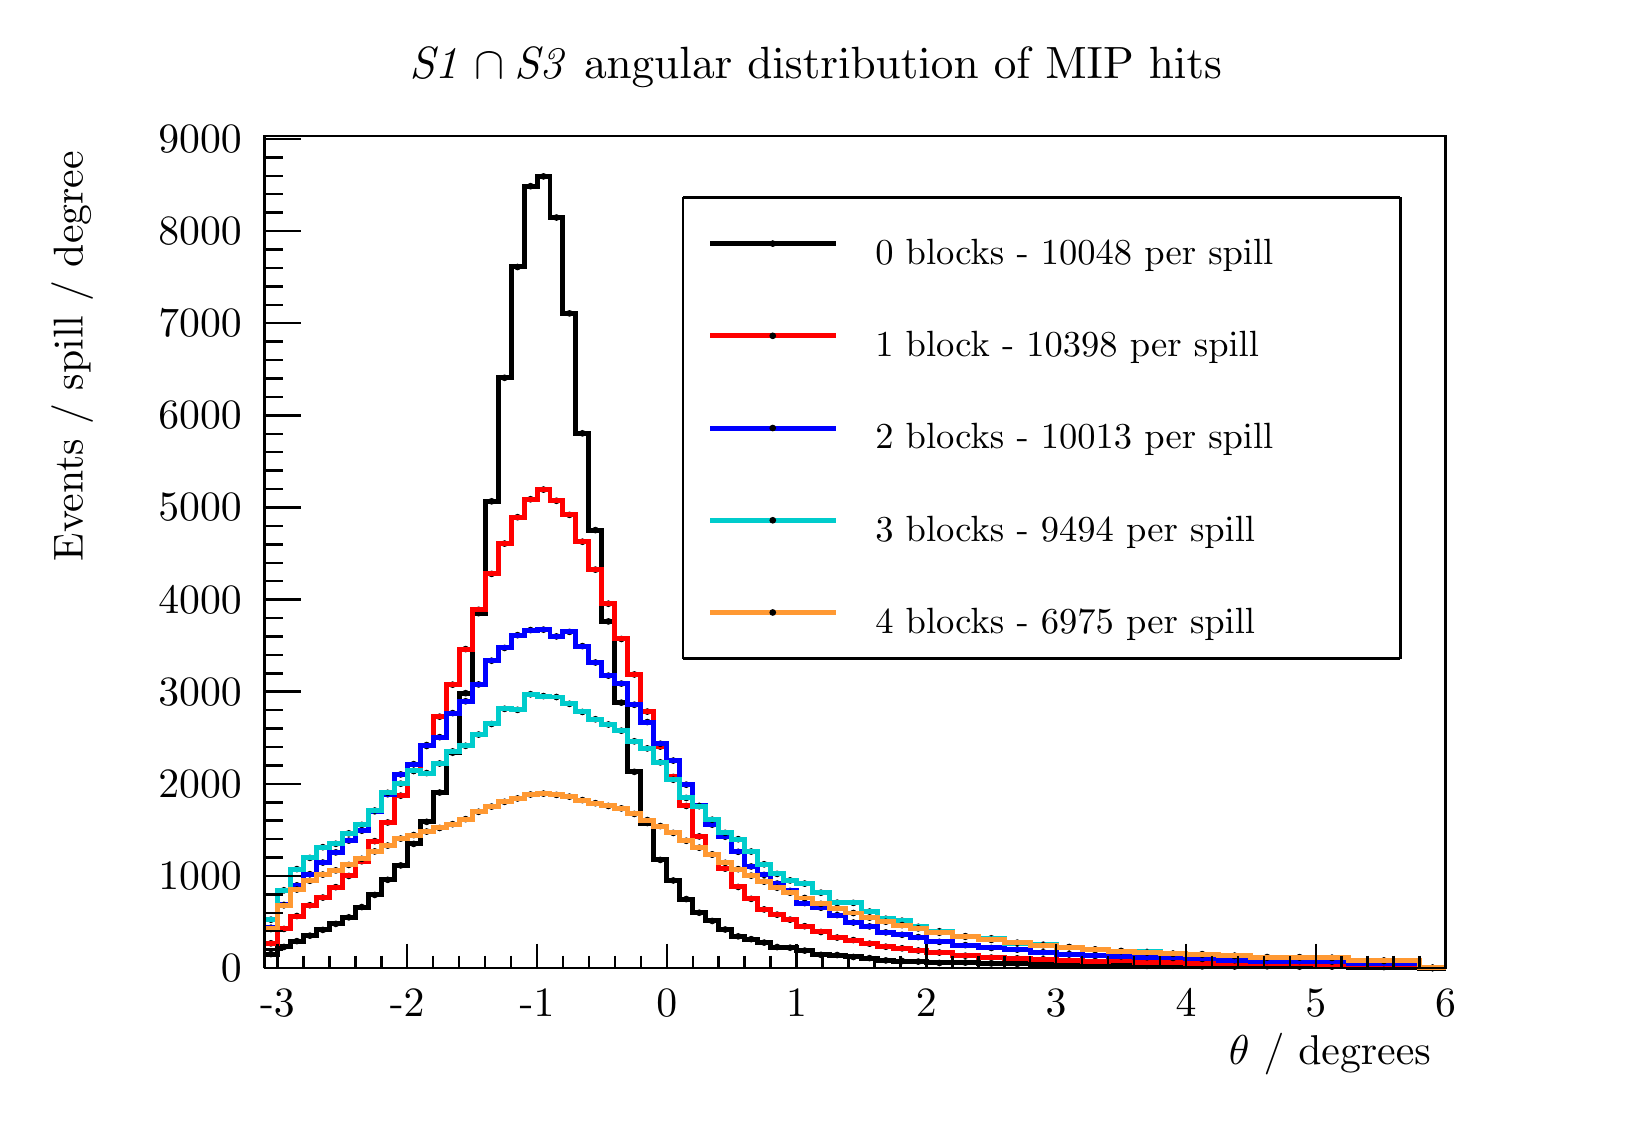
\begin{tikzpicture}
\pgfdeclareplotmark{cross} {
\pgfpathmoveto{\pgfpoint{-0.3\pgfplotmarksize}{\pgfplotmarksize}}
\pgfpathlineto{\pgfpoint{+0.3\pgfplotmarksize}{\pgfplotmarksize}}
\pgfpathlineto{\pgfpoint{+0.3\pgfplotmarksize}{0.3\pgfplotmarksize}}
\pgfpathlineto{\pgfpoint{+1\pgfplotmarksize}{0.3\pgfplotmarksize}}
\pgfpathlineto{\pgfpoint{+1\pgfplotmarksize}{-0.3\pgfplotmarksize}}
\pgfpathlineto{\pgfpoint{+0.3\pgfplotmarksize}{-0.3\pgfplotmarksize}}
\pgfpathlineto{\pgfpoint{+0.3\pgfplotmarksize}{-1.\pgfplotmarksize}}
\pgfpathlineto{\pgfpoint{-0.3\pgfplotmarksize}{-1.\pgfplotmarksize}}
\pgfpathlineto{\pgfpoint{-0.3\pgfplotmarksize}{-0.3\pgfplotmarksize}}
\pgfpathlineto{\pgfpoint{-1.\pgfplotmarksize}{-0.3\pgfplotmarksize}}
\pgfpathlineto{\pgfpoint{-1.\pgfplotmarksize}{0.3\pgfplotmarksize}}
\pgfpathlineto{\pgfpoint{-0.3\pgfplotmarksize}{0.3\pgfplotmarksize}}
\pgfpathclose
\pgfusepathqstroke
}
\pgfdeclareplotmark{cross*} {
\pgfpathmoveto{\pgfpoint{-0.3\pgfplotmarksize}{\pgfplotmarksize}}
\pgfpathlineto{\pgfpoint{+0.3\pgfplotmarksize}{\pgfplotmarksize}}
\pgfpathlineto{\pgfpoint{+0.3\pgfplotmarksize}{0.3\pgfplotmarksize}}
\pgfpathlineto{\pgfpoint{+1\pgfplotmarksize}{0.3\pgfplotmarksize}}
\pgfpathlineto{\pgfpoint{+1\pgfplotmarksize}{-0.3\pgfplotmarksize}}
\pgfpathlineto{\pgfpoint{+0.3\pgfplotmarksize}{-0.3\pgfplotmarksize}}
\pgfpathlineto{\pgfpoint{+0.3\pgfplotmarksize}{-1.\pgfplotmarksize}}
\pgfpathlineto{\pgfpoint{-0.3\pgfplotmarksize}{-1.\pgfplotmarksize}}
\pgfpathlineto{\pgfpoint{-0.3\pgfplotmarksize}{-0.3\pgfplotmarksize}}
\pgfpathlineto{\pgfpoint{-1.\pgfplotmarksize}{-0.3\pgfplotmarksize}}
\pgfpathlineto{\pgfpoint{-1.\pgfplotmarksize}{0.3\pgfplotmarksize}}
\pgfpathlineto{\pgfpoint{-0.3\pgfplotmarksize}{0.3\pgfplotmarksize}}
\pgfpathclose
\pgfusepathqfillstroke
}
\pgfdeclareplotmark{newstar} {
\pgfpathmoveto{\pgfqpoint{0pt}{\pgfplotmarksize}}
\pgfpathlineto{\pgfqpointpolar{44}{0.5\pgfplotmarksize}}
\pgfpathlineto{\pgfqpointpolar{18}{\pgfplotmarksize}}
\pgfpathlineto{\pgfqpointpolar{-20}{0.5\pgfplotmarksize}}
\pgfpathlineto{\pgfqpointpolar{-54}{\pgfplotmarksize}}
\pgfpathlineto{\pgfqpointpolar{-90}{0.5\pgfplotmarksize}}
\pgfpathlineto{\pgfqpointpolar{234}{\pgfplotmarksize}}
\pgfpathlineto{\pgfqpointpolar{198}{0.5\pgfplotmarksize}}
\pgfpathlineto{\pgfqpointpolar{162}{\pgfplotmarksize}}
\pgfpathlineto{\pgfqpointpolar{134}{0.5\pgfplotmarksize}}
\pgfpathclose
\pgfusepathqstroke
}
\pgfdeclareplotmark{newstar*} {
\pgfpathmoveto{\pgfqpoint{0pt}{\pgfplotmarksize}}
\pgfpathlineto{\pgfqpointpolar{44}{0.5\pgfplotmarksize}}
\pgfpathlineto{\pgfqpointpolar{18}{\pgfplotmarksize}}
\pgfpathlineto{\pgfqpointpolar{-20}{0.5\pgfplotmarksize}}
\pgfpathlineto{\pgfqpointpolar{-54}{\pgfplotmarksize}}
\pgfpathlineto{\pgfqpointpolar{-90}{0.5\pgfplotmarksize}}
\pgfpathlineto{\pgfqpointpolar{234}{\pgfplotmarksize}}
\pgfpathlineto{\pgfqpointpolar{198}{0.5\pgfplotmarksize}}
\pgfpathlineto{\pgfqpointpolar{162}{\pgfplotmarksize}}
\pgfpathlineto{\pgfqpointpolar{134}{0.5\pgfplotmarksize}}
\pgfpathclose
\pgfusepathqfillstroke
}
\definecolor{c}{rgb}{1,1,1};
\draw [color=c, fill=c] (0,0) rectangle (20,13.7199);
\draw [color=c, fill=c] (3,1.78359) rectangle (18,12.3479);
\definecolor{c}{rgb}{0,0,0};
\draw [c,line width=0.9] (3,1.78359) -- (3,12.3479) -- (18,12.3479) -- (18,1.78359) -- (3,1.78359);
\definecolor{c}{rgb}{1,1,1};
\draw [color=c, fill=c] (3,1.78359) rectangle (18,12.3479);
\definecolor{c}{rgb}{0,0,0};
\draw [c,line width=0.9] (3,1.78359) -- (3,12.3479) -- (18,12.3479) -- (18,1.78359) -- (3,1.78359);
\definecolor{c}{rgb}{0,0,0.6};
\draw [c,line width=0.9] (3,1.78359) -- (3.16484,1.78359) -- (3.16484,1.78359) -- (3.32967,1.78359) -- (3.32967,1.78359) -- (3.49451,1.78359) -- (3.49451,1.78359) -- (3.65934,1.78359) -- (3.65934,1.78359) -- (3.82418,1.78359) -- (3.82418,1.78359) --
 (3.98901,1.78359) -- (3.98901,1.78359) -- (4.15385,1.78359) -- (4.15385,1.78359) -- (4.31868,1.78359) -- (4.31868,1.78359) -- (4.48352,1.78359) -- (4.48352,1.78359) -- (4.64835,1.78359) -- (4.64835,1.78359) -- (4.81319,1.78359) -- (4.81319,1.78359)
 -- (4.97802,1.78359) -- (4.97802,1.78359) -- (5.14286,1.78359) -- (5.14286,1.78359) -- (5.30769,1.78359) -- (5.30769,1.78359) -- (5.47253,1.78359) -- (5.47253,1.78359) -- (5.63736,1.78359) -- (5.63736,1.78359) -- (5.8022,1.78359) -- (5.8022,1.78359)
 -- (5.96703,1.78359) -- (5.96703,1.78359) -- (6.13187,1.78359) -- (6.13187,1.78359) -- (6.2967,1.78359) -- (6.2967,1.78359) -- (6.46154,1.78359) -- (6.46154,1.78359) -- (6.62637,1.78359) -- (6.62637,1.78359) -- (6.79121,1.78359) -- (6.79121,1.78359)
 -- (6.95604,1.78359) -- (6.95604,1.78359) -- (7.12088,1.78359) -- (7.12088,1.78359) -- (7.28571,1.78359) -- (7.28571,1.78359) -- (7.45055,1.78359) -- (7.45055,1.78359) -- (7.61538,1.78359) -- (7.61538,1.78359) -- (7.78022,1.78359) --
 (7.78022,1.78359) -- (7.94506,1.78359) -- (7.94506,1.78359) -- (8.10989,1.78359) -- (8.10989,1.78359) -- (8.27472,1.78359) -- (8.27472,1.78359) -- (8.43956,1.78359) -- (8.43956,1.78359) -- (8.6044,1.78359) -- (8.6044,1.78359) -- (8.76923,1.78359) --
 (8.76923,1.78359) -- (8.93407,1.78359) -- (8.93407,1.78359) -- (9.0989,1.78359) -- (9.0989,1.78359) -- (9.26374,1.78359) -- (9.26374,1.78359) -- (9.42857,1.78359) -- (9.42857,1.78359) -- (9.59341,1.78359) -- (9.59341,1.78359) -- (9.75824,1.78359) --
 (9.75824,1.78359) -- (9.96429,1.78359) -- (9.96429,1.78359) -- (10.1703,1.78359) -- (10.1703,1.78359) -- (10.3764,1.78359) -- (10.3764,1.78359) -- (10.5824,1.78359) -- (10.5824,1.78359) -- (10.7885,1.78359) -- (10.7885,1.78359) -- (10.9945,1.78359)
 -- (10.9945,1.78359) -- (11.2005,1.78359) -- (11.2005,1.78359) -- (11.4066,1.78359) -- (11.4066,1.78359) -- (11.7363,1.78359) -- (11.7363,1.78359) -- (12.0659,1.78359) -- (12.0659,1.78359) -- (12.3956,1.78359) -- (12.3956,1.78359) --
 (12.7253,1.78359) -- (12.7253,1.78359) -- (13.0549,1.78359) -- (13.0549,1.78359) -- (13.3846,1.78359) -- (13.3846,1.78359) -- (13.7143,1.78359) -- (13.7143,1.78359) -- (14.044,1.78359) -- (14.044,1.78359) -- (14.3736,1.78359) -- (14.3736,1.78359) --
 (14.7033,1.78359) -- (14.7033,1.78359) -- (15.1154,1.78359) -- (15.1154,1.78359) -- (15.5275,1.78359) -- (15.5275,1.78359) -- (15.9396,1.78359) -- (15.9396,1.78359) -- (16.3516,1.78359) -- (16.3516,1.78359) -- (16.7637,1.78359) -- (16.7637,1.78359)
 -- (17.6703,1.78359) -- (17.6703,1.78359) -- (18,1.78359);
\definecolor{c}{rgb}{0,0,0};
\draw [c,line width=0.9] (3,1.78359) -- (18,1.78359);
\draw [c,line width=0.9] (3.16484,2.09229) -- (3.16484,1.78359);
\draw [c,line width=0.9] (3.49451,1.93794) -- (3.49451,1.78359);
\draw [c,line width=0.9] (3.82418,1.93794) -- (3.82418,1.78359);
\draw [c,line width=0.9] (4.15385,1.93794) -- (4.15385,1.78359);
\draw [c,line width=0.9] (4.48352,1.93794) -- (4.48352,1.78359);
\draw [c,line width=0.9] (4.81319,2.09229) -- (4.81319,1.78359);
\draw [c,line width=0.9] (5.14286,1.93794) -- (5.14286,1.78359);
\draw [c,line width=0.9] (5.47253,1.93794) -- (5.47253,1.78359);
\draw [c,line width=0.9] (5.8022,1.93794) -- (5.8022,1.78359);
\draw [c,line width=0.9] (6.13187,1.93794) -- (6.13187,1.78359);
\draw [c,line width=0.9] (6.46154,2.09229) -- (6.46154,1.78359);
\draw [c,line width=0.9] (6.79121,1.93794) -- (6.79121,1.78359);
\draw [c,line width=0.9] (7.12088,1.93794) -- (7.12088,1.78359);
\draw [c,line width=0.9] (7.45055,1.93794) -- (7.45055,1.78359);
\draw [c,line width=0.9] (7.78022,1.93794) -- (7.78022,1.78359);
\draw [c,line width=0.9] (8.10989,2.09229) -- (8.10989,1.78359);
\draw [c,line width=0.9] (8.43956,1.93794) -- (8.43956,1.78359);
\draw [c,line width=0.9] (8.76923,1.93794) -- (8.76923,1.78359);
\draw [c,line width=0.9] (9.0989,1.93794) -- (9.0989,1.78359);
\draw [c,line width=0.9] (9.42857,1.93794) -- (9.42857,1.78359);
\draw [c,line width=0.9] (9.75824,2.09229) -- (9.75824,1.78359);
\draw [c,line width=0.9] (10.0879,1.93794) -- (10.0879,1.78359);
\draw [c,line width=0.9] (10.4176,1.93794) -- (10.4176,1.78359);
\draw [c,line width=0.9] (10.7473,1.93794) -- (10.7473,1.78359);
\draw [c,line width=0.9] (11.0769,1.93794) -- (11.0769,1.78359);
\draw [c,line width=0.9] (11.4066,2.09229) -- (11.4066,1.78359);
\draw [c,line width=0.9] (11.7363,1.93794) -- (11.7363,1.78359);
\draw [c,line width=0.9] (12.0659,1.93794) -- (12.0659,1.78359);
\draw [c,line width=0.9] (12.3956,1.93794) -- (12.3956,1.78359);
\draw [c,line width=0.9] (12.7253,1.93794) -- (12.7253,1.78359);
\draw [c,line width=0.9] (13.0549,2.09229) -- (13.0549,1.78359);
\draw [c,line width=0.9] (13.3846,1.93794) -- (13.3846,1.78359);
\draw [c,line width=0.9] (13.7143,1.93794) -- (13.7143,1.78359);
\draw [c,line width=0.9] (14.044,1.93794) -- (14.044,1.78359);
\draw [c,line width=0.9] (14.3736,1.93794) -- (14.3736,1.78359);
\draw [c,line width=0.9] (14.7033,2.09229) -- (14.7033,1.78359);
\draw [c,line width=0.9] (15.033,1.93794) -- (15.033,1.78359);
\draw [c,line width=0.9] (15.3626,1.93794) -- (15.3626,1.78359);
\draw [c,line width=0.9] (15.6923,1.93794) -- (15.6923,1.78359);
\draw [c,line width=0.9] (16.022,1.93794) -- (16.022,1.78359);
\draw [c,line width=0.9] (16.3516,2.09229) -- (16.3516,1.78359);
\draw [c,line width=0.9] (16.6813,1.93794) -- (16.6813,1.78359);
\draw [c,line width=0.9] (17.011,1.93794) -- (17.011,1.78359);
\draw [c,line width=0.9] (17.3407,1.93794) -- (17.3407,1.78359);
\draw [c,line width=0.9] (17.6703,1.93794) -- (17.6703,1.78359);
\draw [c,line width=0.9] (18,2.09229) -- (18,1.78359);
\draw [c,line width=0.9] (3.16484,2.09229) -- (3.16484,1.78359);
\draw [anchor=base] (3.16484,1.1662) node[scale=1.50787, color=c, rotate=0]{-3};
\draw [anchor=base] (4.81319,1.1662) node[scale=1.50787, color=c, rotate=0]{-2};
\draw [anchor=base] (6.46154,1.1662) node[scale=1.50787, color=c, rotate=0]{-1};
\draw [anchor=base] (8.10989,1.1662) node[scale=1.50787, color=c, rotate=0]{0};
\draw [anchor=base] (9.75824,1.1662) node[scale=1.50787, color=c, rotate=0]{1};
\draw [anchor=base] (11.4066,1.1662) node[scale=1.50787, color=c, rotate=0]{2};
\draw [anchor=base] (13.0549,1.1662) node[scale=1.50787, color=c, rotate=0]{3};
\draw [anchor=base] (14.7033,1.1662) node[scale=1.50787, color=c, rotate=0]{4};
\draw [anchor=base] (16.3516,1.1662) node[scale=1.50787, color=c, rotate=0]{5};
\draw [anchor=base] (18,1.1662) node[scale=1.50787, color=c, rotate=0]{6};
\draw [anchor= east] (18,0.685997) node[scale=1.50787, color=c, rotate=0]{$\theta$ / degrees};
\draw [c,line width=0.9] (3,1.78359) -- (3,12.3479);
\draw [c,line width=0.9] (3.462,1.78359) -- (3,1.78359);
\draw [c,line width=0.9] (3.231,2.01758) -- (3,2.01758);
\draw [c,line width=0.9] (3.231,2.25157) -- (3,2.25157);
\draw [c,line width=0.9] (3.231,2.48557) -- (3,2.48557);
\draw [c,line width=0.9] (3.231,2.71956) -- (3,2.71956);
\draw [c,line width=0.9] (3.462,2.95355) -- (3,2.95355);
\draw [c,line width=0.9] (3.231,3.18754) -- (3,3.18754);
\draw [c,line width=0.9] (3.231,3.42153) -- (3,3.42153);
\draw [c,line width=0.9] (3.231,3.65552) -- (3,3.65552);
\draw [c,line width=0.9] (3.231,3.88951) -- (3,3.88951);
\draw [c,line width=0.9] (3.462,4.1235) -- (3,4.1235);
\draw [c,line width=0.9] (3.231,4.35749) -- (3,4.35749);
\draw [c,line width=0.9] (3.231,4.59148) -- (3,4.59148);
\draw [c,line width=0.9] (3.231,4.82548) -- (3,4.82548);
\draw [c,line width=0.9] (3.231,5.05947) -- (3,5.05947);
\draw [c,line width=0.9] (3.462,5.29346) -- (3,5.29346);
\draw [c,line width=0.9] (3.231,5.52745) -- (3,5.52745);
\draw [c,line width=0.9] (3.231,5.76144) -- (3,5.76144);
\draw [c,line width=0.9] (3.231,5.99543) -- (3,5.99543);
\draw [c,line width=0.9] (3.231,6.22942) -- (3,6.22942);
\draw [c,line width=0.9] (3.462,6.46341) -- (3,6.46341);
\draw [c,line width=0.9] (3.231,6.6974) -- (3,6.6974);
\draw [c,line width=0.9] (3.231,6.93139) -- (3,6.93139);
\draw [c,line width=0.9] (3.231,7.16539) -- (3,7.16539);
\draw [c,line width=0.9] (3.231,7.39938) -- (3,7.39938);
\draw [c,line width=0.9] (3.462,7.63337) -- (3,7.63337);
\draw [c,line width=0.9] (3.231,7.86736) -- (3,7.86736);
\draw [c,line width=0.9] (3.231,8.10135) -- (3,8.10135);
\draw [c,line width=0.9] (3.231,8.33534) -- (3,8.33534);
\draw [c,line width=0.9] (3.231,8.56933) -- (3,8.56933);
\draw [c,line width=0.9] (3.462,8.80332) -- (3,8.80332);
\draw [c,line width=0.9] (3.231,9.03731) -- (3,9.03731);
\draw [c,line width=0.9] (3.231,9.27131) -- (3,9.27131);
\draw [c,line width=0.9] (3.231,9.5053) -- (3,9.5053);
\draw [c,line width=0.9] (3.231,9.73929) -- (3,9.73929);
\draw [c,line width=0.9] (3.462,9.97328) -- (3,9.97328);
\draw [c,line width=0.9] (3.231,10.2073) -- (3,10.2073);
\draw [c,line width=0.9] (3.231,10.4413) -- (3,10.4413);
\draw [c,line width=0.9] (3.231,10.6753) -- (3,10.6753);
\draw [c,line width=0.9] (3.231,10.9092) -- (3,10.9092);
\draw [c,line width=0.9] (3.462,11.1432) -- (3,11.1432);
\draw [c,line width=0.9] (3.231,11.3772) -- (3,11.3772);
\draw [c,line width=0.9] (3.231,11.6112) -- (3,11.6112);
\draw [c,line width=0.9] (3.231,11.8452) -- (3,11.8452);
\draw [c,line width=0.9] (3.231,12.0792) -- (3,12.0792);
\draw [c,line width=0.9] (3.462,12.3132) -- (3,12.3132);
\draw [c,line width=0.9] (3.462,12.3132) -- (3,12.3132);
\draw [anchor= east] (2.9,1.78359) node[scale=1.50787, color=c, rotate=0]{0};
\draw [anchor= east] (2.9,2.95355) node[scale=1.50787, color=c, rotate=0]{1000};
\draw [anchor= east] (2.9,4.1235) node[scale=1.50787, color=c, rotate=0]{2000};
\draw [anchor= east] (2.9,5.29346) node[scale=1.50787, color=c, rotate=0]{3000};
\draw [anchor= east] (2.9,6.46341) node[scale=1.50787, color=c, rotate=0]{4000};
\draw [anchor= east] (2.9,7.63337) node[scale=1.50787, color=c, rotate=0]{5000};
\draw [anchor= east] (2.9,8.80332) node[scale=1.50787, color=c, rotate=0]{6000};
\draw [anchor= east] (2.9,9.97328) node[scale=1.50787, color=c, rotate=0]{7000};
\draw [anchor= east] (2.9,11.1432) node[scale=1.50787, color=c, rotate=0]{8000};
\draw [anchor= east] (2.9,12.3132) node[scale=1.50787, color=c, rotate=0]{9000};
\draw [anchor= east] (0.557284,12.3479) node[scale=1.50787, color=c, rotate=90]{ Events / spill / degree};
\draw [c,line width=1.8] (3.08242,1.96042) -- (3.08242,1.96133);
\draw [c,line width=1.8] (3.08242,1.96133) -- (3.08242,1.96225);
\foreach \P in {(3.08242,1.96133)}{\draw[mark options={color=c,fill=c},mark size=2.402402pt,mark=*,mark size=1pt] plot coordinates {\P};}
\draw [c,line width=1.8] (3.24725,2.05096) -- (3.24725,2.05209);
\draw [c,line width=1.8] (3.24725,2.05209) -- (3.24725,2.05321);
\foreach \P in {(3.24725,2.05209)}{\draw[mark options={color=c,fill=c},mark size=2.402402pt,mark=*,mark size=1pt] plot coordinates {\P};}
\draw [c,line width=1.8] (3.41209,2.1247) -- (3.41209,2.12597);
\draw [c,line width=1.8] (3.41209,2.12597) -- (3.41209,2.12724);
\foreach \P in {(3.41209,2.12597)}{\draw[mark options={color=c,fill=c},mark size=2.402402pt,mark=*,mark size=1pt] plot coordinates {\P};}
\draw [c,line width=1.8] (3.57692,2.19382) -- (3.57692,2.19522);
\draw [c,line width=1.8] (3.57692,2.19522) -- (3.57692,2.19662);
\foreach \P in {(3.57692,2.19522)}{\draw[mark options={color=c,fill=c},mark size=2.402402pt,mark=*,mark size=1pt] plot coordinates {\P};}
\draw [c,line width=1.8] (3.74176,2.26714) -- (3.74176,2.26865);
\draw [c,line width=1.8] (3.74176,2.26865) -- (3.74176,2.27017);
\foreach \P in {(3.74176,2.26865)}{\draw[mark options={color=c,fill=c},mark size=2.402402pt,mark=*,mark size=1pt] plot coordinates {\P};}
\draw [c,line width=1.8] (3.90659,2.34336) -- (3.90659,2.34499);
\draw [c,line width=1.8] (3.90659,2.34499) -- (3.90659,2.34662);
\foreach \P in {(3.90659,2.34499)}{\draw[mark options={color=c,fill=c},mark size=2.402402pt,mark=*,mark size=1pt] plot coordinates {\P};}
\draw [c,line width=1.8] (4.07143,2.42657) -- (4.07143,2.42831);
\draw [c,line width=1.8] (4.07143,2.42831) -- (4.07143,2.43004);
\foreach \P in {(4.07143,2.42831)}{\draw[mark options={color=c,fill=c},mark size=2.402402pt,mark=*,mark size=1pt] plot coordinates {\P};}
\draw [c,line width=1.8] (4.23626,2.55668) -- (4.23626,2.55859);
\draw [c,line width=1.8] (4.23626,2.55859) -- (4.23626,2.5605);
\foreach \P in {(4.23626,2.55859)}{\draw[mark options={color=c,fill=c},mark size=2.402402pt,mark=*,mark size=1pt] plot coordinates {\P};}
\draw [c,line width=1.8] (4.4011,2.71038) -- (4.4011,2.71247);
\draw [c,line width=1.8] (4.4011,2.71247) -- (4.4011,2.71456);
\foreach \P in {(4.4011,2.71247)}{\draw[mark options={color=c,fill=c},mark size=2.402402pt,mark=*,mark size=1pt] plot coordinates {\P};}
\draw [c,line width=1.8] (4.56593,2.90221) -- (4.56593,2.90451);
\draw [c,line width=1.8] (4.56593,2.90451) -- (4.56593,2.90682);
\foreach \P in {(4.56593,2.90451)}{\draw[mark options={color=c,fill=c},mark size=2.402402pt,mark=*,mark size=1pt] plot coordinates {\P};}
\draw [c,line width=1.8] (4.73077,3.08496) -- (4.73077,3.08744);
\draw [c,line width=1.8] (4.73077,3.08744) -- (4.73077,3.08992);
\foreach \P in {(4.73077,3.08744)}{\draw[mark options={color=c,fill=c},mark size=2.402402pt,mark=*,mark size=1pt] plot coordinates {\P};}
\draw [c,line width=1.8] (4.8956,3.35822) -- (4.8956,3.36094);
\draw [c,line width=1.8] (4.8956,3.36094) -- (4.8956,3.36367);
\foreach \P in {(4.8956,3.36094)}{\draw[mark options={color=c,fill=c},mark size=2.402402pt,mark=*,mark size=1pt] plot coordinates {\P};}
\draw [c,line width=1.8] (5.06044,3.63804) -- (5.06044,3.641);
\draw [c,line width=1.8] (5.06044,3.641) -- (5.06044,3.64396);
\foreach \P in {(5.06044,3.641)}{\draw[mark options={color=c,fill=c},mark size=2.402402pt,mark=*,mark size=1pt] plot coordinates {\P};}
\draw [c,line width=1.8] (5.22528,4.00993) -- (5.22528,4.01317);
\draw [c,line width=1.8] (5.22528,4.01317) -- (5.22528,4.01641);
\foreach \P in {(5.22528,4.01317)}{\draw[mark options={color=c,fill=c},mark size=2.402402pt,mark=*,mark size=1pt] plot coordinates {\P};}
\draw [c,line width=1.8] (5.39011,4.5153) -- (5.39011,4.5189);
\draw [c,line width=1.8] (5.39011,4.5189) -- (5.39011,4.52249);
\foreach \P in {(5.39011,4.5189)}{\draw[mark options={color=c,fill=c},mark size=2.402402pt,mark=*,mark size=1pt] plot coordinates {\P};}
\draw [c,line width=1.8] (5.55494,5.27113) -- (5.55494,5.27519);
\draw [c,line width=1.8] (5.55494,5.27519) -- (5.55494,5.27926);
\foreach \P in {(5.55494,5.27519)}{\draw[mark options={color=c,fill=c},mark size=2.402402pt,mark=*,mark size=1pt] plot coordinates {\P};}
\draw [c,line width=1.8] (5.71978,6.28683) -- (5.71978,6.29145);
\draw [c,line width=1.8] (5.71978,6.29145) -- (5.71978,6.29606);
\foreach \P in {(5.71978,6.29145)}{\draw[mark options={color=c,fill=c},mark size=2.402402pt,mark=*,mark size=1pt] plot coordinates {\P};}
\draw [c,line width=1.8] (5.88462,7.70618) -- (5.88462,7.71147);
\draw [c,line width=1.8] (5.88462,7.71147) -- (5.88462,7.71676);
\foreach \P in {(5.88462,7.71147)}{\draw[mark options={color=c,fill=c},mark size=2.402402pt,mark=*,mark size=1pt] plot coordinates {\P};}
\draw [c,line width=1.8] (6.04945,9.27429) -- (6.04945,9.28024);
\draw [c,line width=1.8] (6.04945,9.28024) -- (6.04945,9.28619);
\foreach \P in {(6.04945,9.28024)}{\draw[mark options={color=c,fill=c},mark size=2.402402pt,mark=*,mark size=1pt] plot coordinates {\P};}
\draw [c,line width=1.8] (6.21429,10.681) -- (6.21429,10.6875);
\draw [c,line width=1.8] (6.21429,10.6875) -- (6.21429,10.694);
\foreach \P in {(6.21429,10.6875)}{\draw[mark options={color=c,fill=c},mark size=2.402402pt,mark=*,mark size=1pt] plot coordinates {\P};}
\draw [c,line width=1.8] (6.37912,11.7069) -- (6.37912,11.7137);
\draw [c,line width=1.8] (6.37912,11.7137) -- (6.37912,11.7206);
\foreach \P in {(6.37912,11.7137)}{\draw[mark options={color=c,fill=c},mark size=2.402402pt,mark=*,mark size=1pt] plot coordinates {\P};}
\draw [c,line width=1.8] (6.54396,11.8311) -- (6.54396,11.838);
\draw [c,line width=1.8] (6.54396,11.838) -- (6.54396,11.8449);
\foreach \P in {(6.54396,11.838)}{\draw[mark options={color=c,fill=c},mark size=2.402402pt,mark=*,mark size=1pt] plot coordinates {\P};}
\draw [c,line width=1.8] (6.70879,11.3088) -- (6.70879,11.3155);
\draw [c,line width=1.8] (6.70879,11.3155) -- (6.70879,11.3222);
\foreach \P in {(6.70879,11.3155)}{\draw[mark options={color=c,fill=c},mark size=2.402402pt,mark=*,mark size=1pt] plot coordinates {\P};}
\draw [c,line width=1.8] (6.87363,10.0921) -- (6.87363,10.0984);
\draw [c,line width=1.8] (6.87363,10.0984) -- (6.87363,10.1047);
\foreach \P in {(6.87363,10.0984)}{\draw[mark options={color=c,fill=c},mark size=2.402402pt,mark=*,mark size=1pt] plot coordinates {\P};}
\draw [c,line width=1.8] (7.03846,8.56933) -- (7.03846,8.575);
\draw [c,line width=1.8] (7.03846,8.575) -- (7.03846,8.58066);
\foreach \P in {(7.03846,8.575)}{\draw[mark options={color=c,fill=c},mark size=2.402402pt,mark=*,mark size=1pt] plot coordinates {\P};}
\draw [c,line width=1.8] (7.2033,7.34089) -- (7.2033,7.34602);
\draw [c,line width=1.8] (7.2033,7.34602) -- (7.2033,7.35115);
\foreach \P in {(7.2033,7.34602)}{\draw[mark options={color=c,fill=c},mark size=2.402402pt,mark=*,mark size=1pt] plot coordinates {\P};}
\draw [c,line width=1.8] (7.36813,6.1819) -- (7.36813,6.18646);
\draw [c,line width=1.8] (7.36813,6.18646) -- (7.36813,6.19101);
\foreach \P in {(7.36813,6.18646)}{\draw[mark options={color=c,fill=c},mark size=2.402402pt,mark=*,mark size=1pt] plot coordinates {\P};}
\draw [c,line width=1.8] (7.53297,5.15058) -- (7.53297,5.15457);
\draw [c,line width=1.8] (7.53297,5.15457) -- (7.53297,5.15856);
\foreach \P in {(7.53297,5.15457)}{\draw[mark options={color=c,fill=c},mark size=2.402402pt,mark=*,mark size=1pt] plot coordinates {\P};}
\draw [c,line width=1.8] (7.6978,4.27259) -- (7.6978,4.27602);
\draw [c,line width=1.8] (7.6978,4.27602) -- (7.6978,4.27944);
\foreach \P in {(7.6978,4.27602)}{\draw[mark options={color=c,fill=c},mark size=2.402402pt,mark=*,mark size=1pt] plot coordinates {\P};}
\draw [c,line width=1.8] (7.86264,3.62309) -- (7.86264,3.62604);
\draw [c,line width=1.8] (7.86264,3.62604) -- (7.86264,3.62899);
\foreach \P in {(7.86264,3.62604)}{\draw[mark options={color=c,fill=c},mark size=2.402402pt,mark=*,mark size=1pt] plot coordinates {\P};}
\draw [c,line width=1.8] (8.02747,3.15496) -- (8.02747,3.15751);
\draw [c,line width=1.8] (8.02747,3.15751) -- (8.02747,3.16006);
\foreach \P in {(8.02747,3.15751)}{\draw[mark options={color=c,fill=c},mark size=2.402402pt,mark=*,mark size=1pt] plot coordinates {\P};}
\draw [c,line width=1.8] (8.19231,2.89398) -- (8.19231,2.89627);
\draw [c,line width=1.8] (8.19231,2.89627) -- (8.19231,2.89856);
\foreach \P in {(8.19231,2.89627)}{\draw[mark options={color=c,fill=c},mark size=2.402402pt,mark=*,mark size=1pt] plot coordinates {\P};}
\draw [c,line width=1.8] (8.35714,2.65818) -- (8.35714,2.66022);
\draw [c,line width=1.8] (8.35714,2.66022) -- (8.35714,2.66225);
\foreach \P in {(8.35714,2.66022)}{\draw[mark options={color=c,fill=c},mark size=2.402402pt,mark=*,mark size=1pt] plot coordinates {\P};}
\draw [c,line width=1.8] (8.52198,2.48491) -- (8.52198,2.48674);
\draw [c,line width=1.8] (8.52198,2.48674) -- (8.52198,2.48857);
\foreach \P in {(8.52198,2.48674)}{\draw[mark options={color=c,fill=c},mark size=2.402402pt,mark=*,mark size=1pt] plot coordinates {\P};}
\draw [c,line width=1.8] (8.68681,2.38063) -- (8.68681,2.38232);
\draw [c,line width=1.8] (8.68681,2.38232) -- (8.68681,2.384);
\foreach \P in {(8.68681,2.38232)}{\draw[mark options={color=c,fill=c},mark size=2.402402pt,mark=*,mark size=1pt] plot coordinates {\P};}
\draw [c,line width=1.8] (8.85165,2.272) -- (8.85165,2.27352);
\draw [c,line width=1.8] (8.85165,2.27352) -- (8.85165,2.27504);
\foreach \P in {(8.85165,2.27352)}{\draw[mark options={color=c,fill=c},mark size=2.402402pt,mark=*,mark size=1pt] plot coordinates {\P};}
\draw [c,line width=1.8] (9.01648,2.18553) -- (9.01648,2.18691);
\draw [c,line width=1.8] (9.01648,2.18691) -- (9.01648,2.1883);
\foreach \P in {(9.01648,2.18691)}{\draw[mark options={color=c,fill=c},mark size=2.402402pt,mark=*,mark size=1pt] plot coordinates {\P};}
\draw [c,line width=1.8] (9.18132,2.14992) -- (9.18132,2.15123);
\draw [c,line width=1.8] (9.18132,2.15123) -- (9.18132,2.15255);
\foreach \P in {(9.18132,2.15123)}{\draw[mark options={color=c,fill=c},mark size=2.402402pt,mark=*,mark size=1pt] plot coordinates {\P};}
\draw [c,line width=1.8] (9.34615,2.10613) -- (9.34615,2.10737);
\draw [c,line width=1.8] (9.34615,2.10737) -- (9.34615,2.10861);
\foreach \P in {(9.34615,2.10737)}{\draw[mark options={color=c,fill=c},mark size=2.402402pt,mark=*,mark size=1pt] plot coordinates {\P};}
\draw [c,line width=1.8] (9.51099,2.04971) -- (9.51099,2.05084);
\draw [c,line width=1.8] (9.51099,2.05084) -- (9.51099,2.05196);
\foreach \P in {(9.51099,2.05084)}{\draw[mark options={color=c,fill=c},mark size=2.402402pt,mark=*,mark size=1pt] plot coordinates {\P};}
\draw [c,line width=1.8] (9.67582,2.04139) -- (9.67582,2.0425);
\draw [c,line width=1.8] (9.67582,2.0425) -- (9.67582,2.04362);
\foreach \P in {(9.67582,2.0425)}{\draw[mark options={color=c,fill=c},mark size=2.402402pt,mark=*,mark size=1pt] plot coordinates {\P};}
\draw [c,line width=1.8] (9.86126,2.00446) -- (9.86126,2.0056);
\draw [c,line width=1.8] (9.86126,2.0056) -- (9.86126,2.00675);
\foreach \P in {(9.86126,2.0056)}{\draw[mark options={color=c,fill=c},mark size=2.402402pt,mark=*,mark size=1pt] plot coordinates {\P};}
\draw [c,line width=1.8] (10.0673,1.95095) -- (10.0673,1.95195);
\draw [c,line width=1.8] (10.0673,1.95195) -- (10.0673,1.95295);
\foreach \P in {(10.0673,1.95195)}{\draw[mark options={color=c,fill=c},mark size=2.402402pt,mark=*,mark size=1pt] plot coordinates {\P};}
\draw [c,line width=1.8] (10.2734,1.94837) -- (10.2734,1.94936);
\draw [c,line width=1.8] (10.2734,1.94936) -- (10.2734,1.95035);
\foreach \P in {(10.2734,1.94936)}{\draw[mark options={color=c,fill=c},mark size=2.402402pt,mark=*,mark size=1pt] plot coordinates {\P};}
\draw [c,line width=1.8] (10.4794,1.92407) -- (10.4794,1.92498);
\draw [c,line width=1.8] (10.4794,1.92498) -- (10.4794,1.92589);
\foreach \P in {(10.4794,1.92498)}{\draw[mark options={color=c,fill=c},mark size=2.402402pt,mark=*,mark size=1pt] plot coordinates {\P};}
\draw [c,line width=1.8] (10.6854,1.90959) -- (10.6854,1.91046);
\draw [c,line width=1.8] (10.6854,1.91046) -- (10.6854,1.91133);
\foreach \P in {(10.6854,1.91046)}{\draw[mark options={color=c,fill=c},mark size=2.402402pt,mark=*,mark size=1pt] plot coordinates {\P};}
\draw [c,line width=1.8] (10.8915,1.88035) -- (10.8915,1.88111);
\draw [c,line width=1.8] (10.8915,1.88111) -- (10.8915,1.88187);
\foreach \P in {(10.8915,1.88111)}{\draw[mark options={color=c,fill=c},mark size=2.402402pt,mark=*,mark size=1pt] plot coordinates {\P};}
\draw [c,line width=1.8] (11.0975,1.87278) -- (11.0975,1.87351);
\draw [c,line width=1.8] (11.0975,1.87351) -- (11.0975,1.87424);
\foreach \P in {(11.0975,1.87351)}{\draw[mark options={color=c,fill=c},mark size=2.402402pt,mark=*,mark size=1pt] plot coordinates {\P};}
\draw [c,line width=1.8] (11.3036,1.86516) -- (11.3036,1.86587);
\draw [c,line width=1.8] (11.3036,1.86587) -- (11.3036,1.86657);
\foreach \P in {(11.3036,1.86587)}{\draw[mark options={color=c,fill=c},mark size=2.402402pt,mark=*,mark size=1pt] plot coordinates {\P};}
\draw [c,line width=1.8] (11.5714,1.8481) -- (11.5714,1.84889);
\draw [c,line width=1.8] (11.5714,1.84889) -- (11.5714,1.84967);
\foreach \P in {(11.5714,1.84889)}{\draw[mark options={color=c,fill=c},mark size=2.402402pt,mark=*,mark size=1pt] plot coordinates {\P};}
\draw [c,line width=1.8] (11.9011,1.85223) -- (11.9011,1.85304);
\draw [c,line width=1.8] (11.9011,1.85304) -- (11.9011,1.85385);
\foreach \P in {(11.9011,1.85304)}{\draw[mark options={color=c,fill=c},mark size=2.402402pt,mark=*,mark size=1pt] plot coordinates {\P};}
\draw [c,line width=1.8] (12.2308,1.84206) -- (12.2308,1.84281);
\draw [c,line width=1.8] (12.2308,1.84281) -- (12.2308,1.84356);
\foreach \P in {(12.2308,1.84281)}{\draw[mark options={color=c,fill=c},mark size=2.402402pt,mark=*,mark size=1pt] plot coordinates {\P};}
\draw [c,line width=1.8] (12.5604,1.83622) -- (12.5604,1.83693);
\draw [c,line width=1.8] (12.5604,1.83693) -- (12.5604,1.83764);
\foreach \P in {(12.5604,1.83693)}{\draw[mark options={color=c,fill=c},mark size=2.402402pt,mark=*,mark size=1pt] plot coordinates {\P};}
\draw [c,line width=1.8] (12.8901,1.82585) -- (12.8901,1.82649);
\draw [c,line width=1.8] (12.8901,1.82649) -- (12.8901,1.82713);
\foreach \P in {(12.8901,1.82649)}{\draw[mark options={color=c,fill=c},mark size=2.402402pt,mark=*,mark size=1pt] plot coordinates {\P};}
\draw [c,line width=1.8] (13.2198,1.82341) -- (13.2198,1.82402);
\draw [c,line width=1.8] (13.2198,1.82402) -- (13.2198,1.82464);
\foreach \P in {(13.2198,1.82402)}{\draw[mark options={color=c,fill=c},mark size=2.402402pt,mark=*,mark size=1pt] plot coordinates {\P};}
\draw [c,line width=1.8] (13.5495,1.81898) -- (13.5495,1.81956);
\draw [c,line width=1.8] (13.5495,1.81956) -- (13.5495,1.82014);
\foreach \P in {(13.5495,1.81956)}{\draw[mark options={color=c,fill=c},mark size=2.402402pt,mark=*,mark size=1pt] plot coordinates {\P};}
\draw [c,line width=1.8] (13.8791,1.81696) -- (13.8791,1.81754);
\draw [c,line width=1.8] (13.8791,1.81754) -- (13.8791,1.81812);
\foreach \P in {(13.8791,1.81754)}{\draw[mark options={color=c,fill=c},mark size=2.402402pt,mark=*,mark size=1pt] plot coordinates {\P};}
\draw [c,line width=1.8] (14.2088,1.81084) -- (14.2088,1.81136);
\draw [c,line width=1.8] (14.2088,1.81136) -- (14.2088,1.81187);
\foreach \P in {(14.2088,1.81136)}{\draw[mark options={color=c,fill=c},mark size=2.402402pt,mark=*,mark size=1pt] plot coordinates {\P};}
\draw [c,line width=1.8] (14.5385,1.81226) -- (14.5385,1.81279);
\draw [c,line width=1.8] (14.5385,1.81279) -- (14.5385,1.81331);
\foreach \P in {(14.5385,1.81279)}{\draw[mark options={color=c,fill=c},mark size=2.402402pt,mark=*,mark size=1pt] plot coordinates {\P};}
\draw [c,line width=1.8] (14.9093,1.80551) -- (14.9093,1.80603);
\draw [c,line width=1.8] (14.9093,1.80603) -- (14.9093,1.80656);
\foreach \P in {(14.9093,1.80603)}{\draw[mark options={color=c,fill=c},mark size=2.402402pt,mark=*,mark size=1pt] plot coordinates {\P};}
\draw [c,line width=1.8] (15.3214,1.80324) -- (15.3214,1.80373);
\draw [c,line width=1.8] (15.3214,1.80373) -- (15.3214,1.80421);
\foreach \P in {(15.3214,1.80373)}{\draw[mark options={color=c,fill=c},mark size=2.402402pt,mark=*,mark size=1pt] plot coordinates {\P};}
\draw [c,line width=1.8] (15.7335,1.80624) -- (15.7335,1.80676);
\draw [c,line width=1.8] (15.7335,1.80676) -- (15.7335,1.80729);
\foreach \P in {(15.7335,1.80676)}{\draw[mark options={color=c,fill=c},mark size=2.402402pt,mark=*,mark size=1pt] plot coordinates {\P};}
\draw [c,line width=1.8] (16.1456,1.80134) -- (16.1456,1.8018);
\draw [c,line width=1.8] (16.1456,1.8018) -- (16.1456,1.80227);
\foreach \P in {(16.1456,1.8018)}{\draw[mark options={color=c,fill=c},mark size=2.402402pt,mark=*,mark size=1pt] plot coordinates {\P};}
\draw [c,line width=1.8] (16.5577,1.80172) -- (16.5577,1.80219);
\draw [c,line width=1.8] (16.5577,1.80219) -- (16.5577,1.80265);
\foreach \P in {(16.5577,1.80219)}{\draw[mark options={color=c,fill=c},mark size=2.402402pt,mark=*,mark size=1pt] plot coordinates {\P};}
\draw [c,line width=1.8] (17.217,1.79545) -- (17.217,1.79602);
\draw [c,line width=1.8] (17.217,1.79602) -- (17.217,1.79658);
\foreach \P in {(17.217,1.79602)}{\draw[mark options={color=c,fill=c},mark size=2.402402pt,mark=*,mark size=1pt] plot coordinates {\P};}
\draw [c,line width=1.8] (17.8352,1.78436) -- (17.8352,1.78458);
\draw [c,line width=1.8] (17.8352,1.78458) -- (17.8352,1.7848);
\foreach \P in {(17.8352,1.78458)}{\draw[mark options={color=c,fill=c},mark size=2.402402pt,mark=*,mark size=1pt] plot coordinates {\P};}
\draw [c,line width=1.8] (3,1.96133) -- (3.16484,1.96133) -- (3.16484,2.05209) -- (3.32967,2.05209) -- (3.32967,2.12597) -- (3.49451,2.12597) -- (3.49451,2.19522) -- (3.65934,2.19522) -- (3.65934,2.26865) -- (3.82418,2.26865) -- (3.82418,2.34499) --
 (3.98901,2.34499) -- (3.98901,2.42831) -- (4.15385,2.42831) -- (4.15385,2.55859) -- (4.31868,2.55859) -- (4.31868,2.71247) -- (4.48352,2.71247) -- (4.48352,2.90451) -- (4.64835,2.90451) -- (4.64835,3.08744) -- (4.81319,3.08744) -- (4.81319,3.36094)
 -- (4.97802,3.36094) -- (4.97802,3.641) -- (5.14286,3.641) -- (5.14286,4.01317) -- (5.30769,4.01317) -- (5.30769,4.5189) -- (5.47253,4.5189) -- (5.47253,5.27519) -- (5.63736,5.27519) -- (5.63736,6.29145) -- (5.8022,6.29145) -- (5.8022,7.71147) --
 (5.96703,7.71147) -- (5.96703,9.28024) -- (6.13187,9.28024) -- (6.13187,10.6875) -- (6.2967,10.6875) -- (6.2967,11.7137) -- (6.46154,11.7137) -- (6.46154,11.838) -- (6.62637,11.838) -- (6.62637,11.3155) -- (6.79121,11.3155) -- (6.79121,10.0984) --
 (6.95604,10.0984) -- (6.95604,8.575) -- (7.12088,8.575) -- (7.12088,7.34602) -- (7.28571,7.34602) -- (7.28571,6.18646) -- (7.45055,6.18646) -- (7.45055,5.15457) -- (7.61538,5.15457) -- (7.61538,4.27602) -- (7.78022,4.27602) -- (7.78022,3.62604) --
 (7.94506,3.62604) -- (7.94506,3.15751) -- (8.10989,3.15751) -- (8.10989,2.89627) -- (8.27472,2.89627) -- (8.27472,2.66022) -- (8.43956,2.66022) -- (8.43956,2.48674) -- (8.6044,2.48674) -- (8.6044,2.38232) -- (8.76923,2.38232) -- (8.76923,2.27352) --
 (8.93407,2.27352) -- (8.93407,2.18691) -- (9.0989,2.18691) -- (9.0989,2.15123) -- (9.26374,2.15123) -- (9.26374,2.10737) -- (9.42857,2.10737) -- (9.42857,2.05084) -- (9.59341,2.05084) -- (9.59341,2.0425) -- (9.75824,2.0425) -- (9.75824,2.0056) --
 (9.96429,2.0056) -- (9.96429,1.95195) -- (10.1703,1.95195) -- (10.1703,1.94936) -- (10.3764,1.94936) -- (10.3764,1.92498) -- (10.5824,1.92498) -- (10.5824,1.91046) -- (10.7885,1.91046) -- (10.7885,1.88111) -- (10.9945,1.88111) -- (10.9945,1.87351)
 -- (11.2005,1.87351) -- (11.2005,1.86587) -- (11.4066,1.86587) -- (11.4066,1.84889) -- (11.7363,1.84889) -- (11.7363,1.85304) -- (12.0659,1.85304) -- (12.0659,1.84281) -- (12.3956,1.84281) -- (12.3956,1.83693) -- (12.7253,1.83693) --
 (12.7253,1.82649) -- (13.0549,1.82649) -- (13.0549,1.82402) -- (13.3846,1.82402) -- (13.3846,1.81956) -- (13.7143,1.81956) -- (13.7143,1.81754) -- (14.044,1.81754) -- (14.044,1.81136) -- (14.3736,1.81136) -- (14.3736,1.81279) -- (14.7033,1.81279) --
 (14.7033,1.80603) -- (15.1154,1.80603) -- (15.1154,1.80373) -- (15.5275,1.80373) -- (15.5275,1.80676) -- (15.9396,1.80676) -- (15.9396,1.8018) -- (16.3516,1.8018) -- (16.3516,1.80219) -- (16.7637,1.80219) -- (16.7637,1.79602) -- (17.6703,1.79602) --
 (17.6703,1.78359) -- (18,1.78359);
\definecolor{c}{rgb}{1,0,0};
\draw [c,line width=1.8] (3.08242,2.09714) -- (3.08242,2.09815);
\draw [c,line width=1.8] (3.08242,2.09815) -- (3.08242,2.09916);
\definecolor{c}{rgb}{0,0,0};
\foreach \P in {(3.08242,2.09815)}{\draw[mark options={color=c,fill=c},mark size=2.402402pt,mark=*,mark size=1pt] plot coordinates {\P};}
\definecolor{c}{rgb}{1,0,0};
\draw [c,line width=1.8] (3.24725,2.27948) -- (3.24725,2.28075);
\draw [c,line width=1.8] (3.24725,2.28075) -- (3.24725,2.28201);
\definecolor{c}{rgb}{0,0,0};
\foreach \P in {(3.24725,2.28075)}{\draw[mark options={color=c,fill=c},mark size=2.402402pt,mark=*,mark size=1pt] plot coordinates {\P};}
\definecolor{c}{rgb}{1,0,0};
\draw [c,line width=1.8] (3.41209,2.4435) -- (3.41209,2.44497);
\draw [c,line width=1.8] (3.41209,2.44497) -- (3.41209,2.44643);
\definecolor{c}{rgb}{0,0,0};
\foreach \P in {(3.41209,2.44497)}{\draw[mark options={color=c,fill=c},mark size=2.402402pt,mark=*,mark size=1pt] plot coordinates {\P};}
\definecolor{c}{rgb}{1,0,0};
\draw [c,line width=1.8] (3.57692,2.58039) -- (3.57692,2.582);
\draw [c,line width=1.8] (3.57692,2.582) -- (3.57692,2.58361);
\definecolor{c}{rgb}{0,0,0};
\foreach \P in {(3.57692,2.582)}{\draw[mark options={color=c,fill=c},mark size=2.402402pt,mark=*,mark size=1pt] plot coordinates {\P};}
\definecolor{c}{rgb}{1,0,0};
\draw [c,line width=1.8] (3.74176,2.67742) -- (3.74176,2.67912);
\draw [c,line width=1.8] (3.74176,2.67912) -- (3.74176,2.68082);
\definecolor{c}{rgb}{0,0,0};
\foreach \P in {(3.74176,2.67912)}{\draw[mark options={color=c,fill=c},mark size=2.402402pt,mark=*,mark size=1pt] plot coordinates {\P};}
\definecolor{c}{rgb}{1,0,0};
\draw [c,line width=1.8] (3.90659,2.80977) -- (3.90659,2.8116);
\draw [c,line width=1.8] (3.90659,2.8116) -- (3.90659,2.81342);
\definecolor{c}{rgb}{0,0,0};
\foreach \P in {(3.90659,2.8116)}{\draw[mark options={color=c,fill=c},mark size=2.402402pt,mark=*,mark size=1pt] plot coordinates {\P};}
\definecolor{c}{rgb}{1,0,0};
\draw [c,line width=1.8] (4.07143,2.95225) -- (4.07143,2.9542);
\draw [c,line width=1.8] (4.07143,2.9542) -- (4.07143,2.95615);
\definecolor{c}{rgb}{0,0,0};
\foreach \P in {(4.07143,2.9542)}{\draw[mark options={color=c,fill=c},mark size=2.402402pt,mark=*,mark size=1pt] plot coordinates {\P};}
\definecolor{c}{rgb}{1,0,0};
\draw [c,line width=1.8] (4.23626,3.13862) -- (4.23626,3.14071);
\draw [c,line width=1.8] (4.23626,3.14071) -- (4.23626,3.14281);
\definecolor{c}{rgb}{0,0,0};
\foreach \P in {(4.23626,3.14071)}{\draw[mark options={color=c,fill=c},mark size=2.402402pt,mark=*,mark size=1pt] plot coordinates {\P};}
\definecolor{c}{rgb}{1,0,0};
\draw [c,line width=1.8] (4.4011,3.39362) -- (4.4011,3.39591);
\draw [c,line width=1.8] (4.4011,3.39591) -- (4.4011,3.3982);
\definecolor{c}{rgb}{0,0,0};
\foreach \P in {(4.4011,3.39591)}{\draw[mark options={color=c,fill=c},mark size=2.402402pt,mark=*,mark size=1pt] plot coordinates {\P};}
\definecolor{c}{rgb}{1,0,0};
\draw [c,line width=1.8] (4.56593,3.63056) -- (4.56593,3.63301);
\draw [c,line width=1.8] (4.56593,3.63301) -- (4.56593,3.63546);
\definecolor{c}{rgb}{0,0,0};
\foreach \P in {(4.56593,3.63301)}{\draw[mark options={color=c,fill=c},mark size=2.402402pt,mark=*,mark size=1pt] plot coordinates {\P};}
\definecolor{c}{rgb}{1,0,0};
\draw [c,line width=1.8] (4.73077,3.97085) -- (4.73077,3.97351);
\draw [c,line width=1.8] (4.73077,3.97351) -- (4.73077,3.97617);
\definecolor{c}{rgb}{0,0,0};
\foreach \P in {(4.73077,3.97351)}{\draw[mark options={color=c,fill=c},mark size=2.402402pt,mark=*,mark size=1pt] plot coordinates {\P};}
\definecolor{c}{rgb}{1,0,0};
\draw [c,line width=1.8] (4.8956,4.28388) -- (4.8956,4.28673);
\draw [c,line width=1.8] (4.8956,4.28673) -- (4.8956,4.28957);
\definecolor{c}{rgb}{0,0,0};
\foreach \P in {(4.8956,4.28673)}{\draw[mark options={color=c,fill=c},mark size=2.402402pt,mark=*,mark size=1pt] plot coordinates {\P};}
\definecolor{c}{rgb}{1,0,0};
\draw [c,line width=1.8] (5.06044,4.6015) -- (5.06044,4.60452);
\draw [c,line width=1.8] (5.06044,4.60452) -- (5.06044,4.60754);
\definecolor{c}{rgb}{0,0,0};
\foreach \P in {(5.06044,4.60452)}{\draw[mark options={color=c,fill=c},mark size=2.402402pt,mark=*,mark size=1pt] plot coordinates {\P};}
\definecolor{c}{rgb}{1,0,0};
\draw [c,line width=1.8] (5.22528,4.97306) -- (5.22528,4.97628);
\draw [c,line width=1.8] (5.22528,4.97628) -- (5.22528,4.97949);
\definecolor{c}{rgb}{0,0,0};
\foreach \P in {(5.22528,4.97628)}{\draw[mark options={color=c,fill=c},mark size=2.402402pt,mark=*,mark size=1pt] plot coordinates {\P};}
\definecolor{c}{rgb}{1,0,0};
\draw [c,line width=1.8] (5.39011,5.37934) -- (5.39011,5.38275);
\draw [c,line width=1.8] (5.39011,5.38275) -- (5.39011,5.38617);
\definecolor{c}{rgb}{0,0,0};
\foreach \P in {(5.39011,5.38275)}{\draw[mark options={color=c,fill=c},mark size=2.402402pt,mark=*,mark size=1pt] plot coordinates {\P};}
\definecolor{c}{rgb}{1,0,0};
\draw [c,line width=1.8] (5.55494,5.83124) -- (5.55494,5.83486);
\draw [c,line width=1.8] (5.55494,5.83486) -- (5.55494,5.83847);
\definecolor{c}{rgb}{0,0,0};
\foreach \P in {(5.55494,5.83486)}{\draw[mark options={color=c,fill=c},mark size=2.402402pt,mark=*,mark size=1pt] plot coordinates {\P};}
\definecolor{c}{rgb}{1,0,0};
\draw [c,line width=1.8] (5.71978,6.32959) -- (5.71978,6.33342);
\draw [c,line width=1.8] (5.71978,6.33342) -- (5.71978,6.33725);
\definecolor{c}{rgb}{0,0,0};
\foreach \P in {(5.71978,6.33342)}{\draw[mark options={color=c,fill=c},mark size=2.402402pt,mark=*,mark size=1pt] plot coordinates {\P};}
\definecolor{c}{rgb}{1,0,0};
\draw [c,line width=1.8] (5.88462,6.78597) -- (5.88462,6.78999);
\draw [c,line width=1.8] (5.88462,6.78999) -- (5.88462,6.79401);
\definecolor{c}{rgb}{0,0,0};
\foreach \P in {(5.88462,6.78999)}{\draw[mark options={color=c,fill=c},mark size=2.402402pt,mark=*,mark size=1pt] plot coordinates {\P};}
\definecolor{c}{rgb}{1,0,0};
\draw [c,line width=1.8] (6.04945,7.1706) -- (6.04945,7.17477);
\draw [c,line width=1.8] (6.04945,7.17477) -- (6.04945,7.17894);
\definecolor{c}{rgb}{0,0,0};
\foreach \P in {(6.04945,7.17477)}{\draw[mark options={color=c,fill=c},mark size=2.402402pt,mark=*,mark size=1pt] plot coordinates {\P};}
\definecolor{c}{rgb}{1,0,0};
\draw [c,line width=1.8] (6.21429,7.50559) -- (6.21429,7.50989);
\draw [c,line width=1.8] (6.21429,7.50989) -- (6.21429,7.51419);
\definecolor{c}{rgb}{0,0,0};
\foreach \P in {(6.21429,7.50989)}{\draw[mark options={color=c,fill=c},mark size=2.402402pt,mark=*,mark size=1pt] plot coordinates {\P};}
\definecolor{c}{rgb}{1,0,0};
\draw [c,line width=1.8] (6.37912,7.73355) -- (6.37912,7.73794);
\draw [c,line width=1.8] (6.37912,7.73794) -- (6.37912,7.74233);
\definecolor{c}{rgb}{0,0,0};
\foreach \P in {(6.37912,7.73794)}{\draw[mark options={color=c,fill=c},mark size=2.402402pt,mark=*,mark size=1pt] plot coordinates {\P};}
\definecolor{c}{rgb}{1,0,0};
\draw [c,line width=1.8] (6.54396,7.856) -- (6.54396,7.86043);
\draw [c,line width=1.8] (6.54396,7.86043) -- (6.54396,7.86486);
\definecolor{c}{rgb}{0,0,0};
\foreach \P in {(6.54396,7.86043)}{\draw[mark options={color=c,fill=c},mark size=2.402402pt,mark=*,mark size=1pt] plot coordinates {\P};}
\definecolor{c}{rgb}{1,0,0};
\draw [c,line width=1.8] (6.70879,7.71375) -- (6.70879,7.71814);
\draw [c,line width=1.8] (6.70879,7.71814) -- (6.70879,7.72252);
\definecolor{c}{rgb}{0,0,0};
\foreach \P in {(6.70879,7.71814)}{\draw[mark options={color=c,fill=c},mark size=2.402402pt,mark=*,mark size=1pt] plot coordinates {\P};}
\definecolor{c}{rgb}{1,0,0};
\draw [c,line width=1.8] (6.87363,7.53514) -- (6.87363,7.53945);
\draw [c,line width=1.8] (6.87363,7.53945) -- (6.87363,7.54376);
\definecolor{c}{rgb}{0,0,0};
\foreach \P in {(6.87363,7.53945)}{\draw[mark options={color=c,fill=c},mark size=2.402402pt,mark=*,mark size=1pt] plot coordinates {\P};}
\definecolor{c}{rgb}{1,0,0};
\draw [c,line width=1.8] (7.03846,7.1942) -- (7.03846,7.19838);
\draw [c,line width=1.8] (7.03846,7.19838) -- (7.03846,7.20256);
\definecolor{c}{rgb}{0,0,0};
\foreach \P in {(7.03846,7.19838)}{\draw[mark options={color=c,fill=c},mark size=2.402402pt,mark=*,mark size=1pt] plot coordinates {\P};}
\definecolor{c}{rgb}{1,0,0};
\draw [c,line width=1.8] (7.2033,6.8398) -- (7.2033,6.84384);
\draw [c,line width=1.8] (7.2033,6.84384) -- (7.2033,6.84788);
\definecolor{c}{rgb}{0,0,0};
\foreach \P in {(7.2033,6.84384)}{\draw[mark options={color=c,fill=c},mark size=2.402402pt,mark=*,mark size=1pt] plot coordinates {\P};}
\definecolor{c}{rgb}{1,0,0};
\draw [c,line width=1.8] (7.36813,6.40726) -- (7.36813,6.41113);
\draw [c,line width=1.8] (7.36813,6.41113) -- (7.36813,6.41499);
\definecolor{c}{rgb}{0,0,0};
\foreach \P in {(7.36813,6.41113)}{\draw[mark options={color=c,fill=c},mark size=2.402402pt,mark=*,mark size=1pt] plot coordinates {\P};}
\definecolor{c}{rgb}{1,0,0};
\draw [c,line width=1.8] (7.53297,5.95964) -- (7.53297,5.96331);
\draw [c,line width=1.8] (7.53297,5.96331) -- (7.53297,5.96699);
\definecolor{c}{rgb}{0,0,0};
\foreach \P in {(7.53297,5.96331)}{\draw[mark options={color=c,fill=c},mark size=2.402402pt,mark=*,mark size=1pt] plot coordinates {\P};}
\definecolor{c}{rgb}{1,0,0};
\draw [c,line width=1.8] (7.6978,5.50906) -- (7.6978,5.51253);
\draw [c,line width=1.8] (7.6978,5.51253) -- (7.6978,5.51599);
\definecolor{c}{rgb}{0,0,0};
\foreach \P in {(7.6978,5.51253)}{\draw[mark options={color=c,fill=c},mark size=2.402402pt,mark=*,mark size=1pt] plot coordinates {\P};}
\definecolor{c}{rgb}{1,0,0};
\draw [c,line width=1.8] (7.86264,5.03779) -- (7.86264,5.04103);
\draw [c,line width=1.8] (7.86264,5.04103) -- (7.86264,5.04427);
\definecolor{c}{rgb}{0,0,0};
\foreach \P in {(7.86264,5.04103)}{\draw[mark options={color=c,fill=c},mark size=2.402402pt,mark=*,mark size=1pt] plot coordinates {\P};}
\definecolor{c}{rgb}{1,0,0};
\draw [c,line width=1.8] (8.02747,4.59326) -- (8.02747,4.59628);
\draw [c,line width=1.8] (8.02747,4.59628) -- (8.02747,4.59929);
\definecolor{c}{rgb}{0,0,0};
\foreach \P in {(8.02747,4.59628)}{\draw[mark options={color=c,fill=c},mark size=2.402402pt,mark=*,mark size=1pt] plot coordinates {\P};}
\definecolor{c}{rgb}{1,0,0};
\draw [c,line width=1.8] (8.19231,4.20832) -- (8.19231,4.21113);
\draw [c,line width=1.8] (8.19231,4.21113) -- (8.19231,4.21393);
\definecolor{c}{rgb}{0,0,0};
\foreach \P in {(8.19231,4.21113)}{\draw[mark options={color=c,fill=c},mark size=2.402402pt,mark=*,mark size=1pt] plot coordinates {\P};}
\definecolor{c}{rgb}{1,0,0};
\draw [c,line width=1.8] (8.35714,3.84025) -- (8.35714,3.84283);
\draw [c,line width=1.8] (8.35714,3.84283) -- (8.35714,3.8454);
\definecolor{c}{rgb}{0,0,0};
\foreach \P in {(8.35714,3.84283)}{\draw[mark options={color=c,fill=c},mark size=2.402402pt,mark=*,mark size=1pt] plot coordinates {\P};}
\definecolor{c}{rgb}{1,0,0};
\draw [c,line width=1.8] (8.52198,3.45334) -- (8.52198,3.45567);
\draw [c,line width=1.8] (8.52198,3.45567) -- (8.52198,3.45799);
\definecolor{c}{rgb}{0,0,0};
\foreach \P in {(8.52198,3.45567)}{\draw[mark options={color=c,fill=c},mark size=2.402402pt,mark=*,mark size=1pt] plot coordinates {\P};}
\definecolor{c}{rgb}{1,0,0};
\draw [c,line width=1.8] (8.68681,3.2251) -- (8.68681,3.22726);
\draw [c,line width=1.8] (8.68681,3.22726) -- (8.68681,3.22942);
\definecolor{c}{rgb}{0,0,0};
\foreach \P in {(8.68681,3.22726)}{\draw[mark options={color=c,fill=c},mark size=2.402402pt,mark=*,mark size=1pt] plot coordinates {\P};}
\definecolor{c}{rgb}{1,0,0};
\draw [c,line width=1.8] (8.85165,3.04516) -- (8.85165,3.04718);
\draw [c,line width=1.8] (8.85165,3.04718) -- (8.85165,3.0492);
\definecolor{c}{rgb}{0,0,0};
\foreach \P in {(8.85165,3.04718)}{\draw[mark options={color=c,fill=c},mark size=2.402402pt,mark=*,mark size=1pt] plot coordinates {\P};}
\definecolor{c}{rgb}{1,0,0};
\draw [c,line width=1.8] (9.01648,2.81245) -- (9.01648,2.81428);
\draw [c,line width=1.8] (9.01648,2.81428) -- (9.01648,2.81611);
\definecolor{c}{rgb}{0,0,0};
\foreach \P in {(9.01648,2.81428)}{\draw[mark options={color=c,fill=c},mark size=2.402402pt,mark=*,mark size=1pt] plot coordinates {\P};}
\definecolor{c}{rgb}{1,0,0};
\draw [c,line width=1.8] (9.18132,2.66138) -- (9.18132,2.66306);
\draw [c,line width=1.8] (9.18132,2.66306) -- (9.18132,2.66475);
\definecolor{c}{rgb}{0,0,0};
\foreach \P in {(9.18132,2.66306)}{\draw[mark options={color=c,fill=c},mark size=2.402402pt,mark=*,mark size=1pt] plot coordinates {\P};}
\definecolor{c}{rgb}{1,0,0};
\draw [c,line width=1.8] (9.34615,2.52706) -- (9.34615,2.52861);
\draw [c,line width=1.8] (9.34615,2.52861) -- (9.34615,2.53016);
\definecolor{c}{rgb}{0,0,0};
\foreach \P in {(9.34615,2.52861)}{\draw[mark options={color=c,fill=c},mark size=2.402402pt,mark=*,mark size=1pt] plot coordinates {\P};}
\definecolor{c}{rgb}{1,0,0};
\draw [c,line width=1.8] (9.51099,2.46034) -- (9.51099,2.46183);
\draw [c,line width=1.8] (9.51099,2.46183) -- (9.51099,2.46331);
\definecolor{c}{rgb}{0,0,0};
\foreach \P in {(9.51099,2.46183)}{\draw[mark options={color=c,fill=c},mark size=2.402402pt,mark=*,mark size=1pt] plot coordinates {\P};}
\definecolor{c}{rgb}{1,0,0};
\draw [c,line width=1.8] (9.67582,2.3973) -- (9.67582,2.39871);
\draw [c,line width=1.8] (9.67582,2.39871) -- (9.67582,2.40012);
\definecolor{c}{rgb}{0,0,0};
\foreach \P in {(9.67582,2.39871)}{\draw[mark options={color=c,fill=c},mark size=2.402402pt,mark=*,mark size=1pt] plot coordinates {\P};}
\definecolor{c}{rgb}{1,0,0};
\draw [c,line width=1.8] (9.86126,2.31431) -- (9.86126,2.31578);
\draw [c,line width=1.8] (9.86126,2.31578) -- (9.86126,2.31724);
\definecolor{c}{rgb}{0,0,0};
\foreach \P in {(9.86126,2.31578)}{\draw[mark options={color=c,fill=c},mark size=2.402402pt,mark=*,mark size=1pt] plot coordinates {\P};}
\definecolor{c}{rgb}{1,0,0};
\draw [c,line width=1.8] (10.0673,2.24077) -- (10.0673,2.24213);
\draw [c,line width=1.8] (10.0673,2.24213) -- (10.0673,2.24349);
\definecolor{c}{rgb}{0,0,0};
\foreach \P in {(10.0673,2.24213)}{\draw[mark options={color=c,fill=c},mark size=2.402402pt,mark=*,mark size=1pt] plot coordinates {\P};}
\definecolor{c}{rgb}{1,0,0};
\draw [c,line width=1.8] (10.2734,2.16998) -- (10.2734,2.17124);
\draw [c,line width=1.8] (10.2734,2.17124) -- (10.2734,2.17249);
\definecolor{c}{rgb}{0,0,0};
\foreach \P in {(10.2734,2.17124)}{\draw[mark options={color=c,fill=c},mark size=2.402402pt,mark=*,mark size=1pt] plot coordinates {\P};}
\definecolor{c}{rgb}{1,0,0};
\draw [c,line width=1.8] (10.4794,2.13818) -- (10.4794,2.13938);
\draw [c,line width=1.8] (10.4794,2.13938) -- (10.4794,2.14058);
\definecolor{c}{rgb}{0,0,0};
\foreach \P in {(10.4794,2.13938)}{\draw[mark options={color=c,fill=c},mark size=2.402402pt,mark=*,mark size=1pt] plot coordinates {\P};}
\definecolor{c}{rgb}{1,0,0};
\draw [c,line width=1.8] (10.6854,2.09282) -- (10.6854,2.09394);
\draw [c,line width=1.8] (10.6854,2.09394) -- (10.6854,2.09507);
\definecolor{c}{rgb}{0,0,0};
\foreach \P in {(10.6854,2.09394)}{\draw[mark options={color=c,fill=c},mark size=2.402402pt,mark=*,mark size=1pt] plot coordinates {\P};}
\definecolor{c}{rgb}{1,0,0};
\draw [c,line width=1.8] (10.8915,2.05389) -- (10.8915,2.05493);
\draw [c,line width=1.8] (10.8915,2.05493) -- (10.8915,2.05597);
\definecolor{c}{rgb}{0,0,0};
\foreach \P in {(10.8915,2.05493)}{\draw[mark options={color=c,fill=c},mark size=2.402402pt,mark=*,mark size=1pt] plot coordinates {\P};}
\definecolor{c}{rgb}{1,0,0};
\draw [c,line width=1.8] (11.0975,2.03371) -- (11.0975,2.03472);
\draw [c,line width=1.8] (11.0975,2.03472) -- (11.0975,2.03572);
\definecolor{c}{rgb}{0,0,0};
\foreach \P in {(11.0975,2.03472)}{\draw[mark options={color=c,fill=c},mark size=2.402402pt,mark=*,mark size=1pt] plot coordinates {\P};}
\definecolor{c}{rgb}{1,0,0};
\draw [c,line width=1.8] (11.3036,2.00608) -- (11.3036,2.00703);
\draw [c,line width=1.8] (11.3036,2.00703) -- (11.3036,2.00797);
\definecolor{c}{rgb}{0,0,0};
\foreach \P in {(11.3036,2.00703)}{\draw[mark options={color=c,fill=c},mark size=2.402402pt,mark=*,mark size=1pt] plot coordinates {\P};}
\definecolor{c}{rgb}{1,0,0};
\draw [c,line width=1.8] (11.5714,1.97989) -- (11.5714,1.98102);
\draw [c,line width=1.8] (11.5714,1.98102) -- (11.5714,1.98214);
\definecolor{c}{rgb}{0,0,0};
\foreach \P in {(11.5714,1.98102)}{\draw[mark options={color=c,fill=c},mark size=2.402402pt,mark=*,mark size=1pt] plot coordinates {\P};}
\definecolor{c}{rgb}{1,0,0};
\draw [c,line width=1.8] (11.9011,1.93989) -- (11.9011,1.9409);
\draw [c,line width=1.8] (11.9011,1.9409) -- (11.9011,1.94191);
\definecolor{c}{rgb}{0,0,0};
\foreach \P in {(11.9011,1.9409)}{\draw[mark options={color=c,fill=c},mark size=2.402402pt,mark=*,mark size=1pt] plot coordinates {\P};}
\definecolor{c}{rgb}{1,0,0};
\draw [c,line width=1.8] (12.2308,1.91581) -- (12.2308,1.91674);
\draw [c,line width=1.8] (12.2308,1.91674) -- (12.2308,1.91767);
\definecolor{c}{rgb}{0,0,0};
\foreach \P in {(12.2308,1.91674)}{\draw[mark options={color=c,fill=c},mark size=2.402402pt,mark=*,mark size=1pt] plot coordinates {\P};}
\definecolor{c}{rgb}{1,0,0};
\draw [c,line width=1.8] (12.5604,1.90642) -- (12.5604,1.90732);
\draw [c,line width=1.8] (12.5604,1.90732) -- (12.5604,1.90821);
\definecolor{c}{rgb}{0,0,0};
\foreach \P in {(12.5604,1.90732)}{\draw[mark options={color=c,fill=c},mark size=2.402402pt,mark=*,mark size=1pt] plot coordinates {\P};}
\definecolor{c}{rgb}{1,0,0};
\draw [c,line width=1.8] (12.8901,1.89523) -- (12.8901,1.89609);
\draw [c,line width=1.8] (12.8901,1.89609) -- (12.8901,1.89694);
\definecolor{c}{rgb}{0,0,0};
\foreach \P in {(12.8901,1.89609)}{\draw[mark options={color=c,fill=c},mark size=2.402402pt,mark=*,mark size=1pt] plot coordinates {\P};}
\definecolor{c}{rgb}{1,0,0};
\draw [c,line width=1.8] (13.2198,1.87942) -- (13.2198,1.88021);
\draw [c,line width=1.8] (13.2198,1.88021) -- (13.2198,1.881);
\definecolor{c}{rgb}{0,0,0};
\foreach \P in {(13.2198,1.88021)}{\draw[mark options={color=c,fill=c},mark size=2.402402pt,mark=*,mark size=1pt] plot coordinates {\P};}
\definecolor{c}{rgb}{1,0,0};
\draw [c,line width=1.8] (13.5495,1.87219) -- (13.5495,1.87295);
\draw [c,line width=1.8] (13.5495,1.87295) -- (13.5495,1.87371);
\definecolor{c}{rgb}{0,0,0};
\foreach \P in {(13.5495,1.87295)}{\draw[mark options={color=c,fill=c},mark size=2.402402pt,mark=*,mark size=1pt] plot coordinates {\P};}
\definecolor{c}{rgb}{1,0,0};
\draw [c,line width=1.8] (13.8791,1.87478) -- (13.8791,1.87555);
\draw [c,line width=1.8] (13.8791,1.87555) -- (13.8791,1.87632);
\definecolor{c}{rgb}{0,0,0};
\foreach \P in {(13.8791,1.87555)}{\draw[mark options={color=c,fill=c},mark size=2.402402pt,mark=*,mark size=1pt] plot coordinates {\P};}
\definecolor{c}{rgb}{1,0,0};
\draw [c,line width=1.8] (14.2088,1.85406) -- (14.2088,1.85474);
\draw [c,line width=1.8] (14.2088,1.85474) -- (14.2088,1.85542);
\definecolor{c}{rgb}{0,0,0};
\foreach \P in {(14.2088,1.85474)}{\draw[mark options={color=c,fill=c},mark size=2.402402pt,mark=*,mark size=1pt] plot coordinates {\P};}
\definecolor{c}{rgb}{1,0,0};
\draw [c,line width=1.8] (14.5385,1.85869) -- (14.5385,1.85938);
\draw [c,line width=1.8] (14.5385,1.85938) -- (14.5385,1.86008);
\definecolor{c}{rgb}{0,0,0};
\foreach \P in {(14.5385,1.85938)}{\draw[mark options={color=c,fill=c},mark size=2.402402pt,mark=*,mark size=1pt] plot coordinates {\P};}
\definecolor{c}{rgb}{1,0,0};
\draw [c,line width=1.8] (14.9093,1.8404) -- (14.9093,1.84108);
\draw [c,line width=1.8] (14.9093,1.84108) -- (14.9093,1.84177);
\definecolor{c}{rgb}{0,0,0};
\foreach \P in {(14.9093,1.84108)}{\draw[mark options={color=c,fill=c},mark size=2.402402pt,mark=*,mark size=1pt] plot coordinates {\P};}
\definecolor{c}{rgb}{1,0,0};
\draw [c,line width=1.8] (15.3214,1.84042) -- (15.3214,1.84111);
\draw [c,line width=1.8] (15.3214,1.84111) -- (15.3214,1.84179);
\definecolor{c}{rgb}{0,0,0};
\foreach \P in {(15.3214,1.84111)}{\draw[mark options={color=c,fill=c},mark size=2.402402pt,mark=*,mark size=1pt] plot coordinates {\P};}
\definecolor{c}{rgb}{1,0,0};
\draw [c,line width=1.8] (15.7335,1.83506) -- (15.7335,1.83571);
\draw [c,line width=1.8] (15.7335,1.83571) -- (15.7335,1.83636);
\definecolor{c}{rgb}{0,0,0};
\foreach \P in {(15.7335,1.83571)}{\draw[mark options={color=c,fill=c},mark size=2.402402pt,mark=*,mark size=1pt] plot coordinates {\P};}
\definecolor{c}{rgb}{1,0,0};
\draw [c,line width=1.8] (16.1456,1.83527) -- (16.1456,1.83591);
\draw [c,line width=1.8] (16.1456,1.83591) -- (16.1456,1.83656);
\definecolor{c}{rgb}{0,0,0};
\foreach \P in {(16.1456,1.83591)}{\draw[mark options={color=c,fill=c},mark size=2.402402pt,mark=*,mark size=1pt] plot coordinates {\P};}
\definecolor{c}{rgb}{1,0,0};
\draw [c,line width=1.8] (16.5577,1.83409) -- (16.5577,1.83473);
\draw [c,line width=1.8] (16.5577,1.83473) -- (16.5577,1.83538);
\definecolor{c}{rgb}{0,0,0};
\foreach \P in {(16.5577,1.83473)}{\draw[mark options={color=c,fill=c},mark size=2.402402pt,mark=*,mark size=1pt] plot coordinates {\P};}
\definecolor{c}{rgb}{1,0,0};
\draw [c,line width=1.8] (17.217,1.81844) -- (17.217,1.81924);
\draw [c,line width=1.8] (17.217,1.81924) -- (17.217,1.82004);
\definecolor{c}{rgb}{0,0,0};
\foreach \P in {(17.217,1.81924)}{\draw[mark options={color=c,fill=c},mark size=2.402402pt,mark=*,mark size=1pt] plot coordinates {\P};}
\definecolor{c}{rgb}{1,0,0};
\draw [c,line width=1.8] (17.8352,1.7846) -- (17.8352,1.7848);
\draw [c,line width=1.8] (17.8352,1.7848) -- (17.8352,1.785);
\definecolor{c}{rgb}{0,0,0};
\foreach \P in {(17.8352,1.7848)}{\draw[mark options={color=c,fill=c},mark size=2.402402pt,mark=*,mark size=1pt] plot coordinates {\P};}
\definecolor{c}{rgb}{1,0,0};
\draw [c,line width=1.8] (3,2.09815) -- (3.16484,2.09815) -- (3.16484,2.28075) -- (3.32967,2.28075) -- (3.32967,2.44497) -- (3.49451,2.44497) -- (3.49451,2.582) -- (3.65934,2.582) -- (3.65934,2.67912) -- (3.82418,2.67912) -- (3.82418,2.8116) --
 (3.98901,2.8116) -- (3.98901,2.9542) -- (4.15385,2.9542) -- (4.15385,3.14071) -- (4.31868,3.14071) -- (4.31868,3.39591) -- (4.48352,3.39591) -- (4.48352,3.63301) -- (4.64835,3.63301) -- (4.64835,3.97351) -- (4.81319,3.97351) -- (4.81319,4.28673) --
 (4.97802,4.28673) -- (4.97802,4.60452) -- (5.14286,4.60452) -- (5.14286,4.97628) -- (5.30769,4.97628) -- (5.30769,5.38275) -- (5.47253,5.38275) -- (5.47253,5.83486) -- (5.63736,5.83486) -- (5.63736,6.33342) -- (5.8022,6.33342) -- (5.8022,6.78999) --
 (5.96703,6.78999) -- (5.96703,7.17477) -- (6.13187,7.17477) -- (6.13187,7.50989) -- (6.2967,7.50989) -- (6.2967,7.73794) -- (6.46154,7.73794) -- (6.46154,7.86043) -- (6.62637,7.86043) -- (6.62637,7.71814) -- (6.79121,7.71814) -- (6.79121,7.53945) --
 (6.95604,7.53945) -- (6.95604,7.19838) -- (7.12088,7.19838) -- (7.12088,6.84384) -- (7.28571,6.84384) -- (7.28571,6.41113) -- (7.45055,6.41113) -- (7.45055,5.96331) -- (7.61538,5.96331) -- (7.61538,5.51253) -- (7.78022,5.51253) -- (7.78022,5.04103)
 -- (7.94506,5.04103) -- (7.94506,4.59628) -- (8.10989,4.59628) -- (8.10989,4.21113) -- (8.27472,4.21113) -- (8.27472,3.84283) -- (8.43956,3.84283) -- (8.43956,3.45567) -- (8.6044,3.45567) -- (8.6044,3.22726) -- (8.76923,3.22726) -- (8.76923,3.04718)
 -- (8.93407,3.04718) -- (8.93407,2.81428) -- (9.0989,2.81428) -- (9.0989,2.66306) -- (9.26374,2.66306) -- (9.26374,2.52861) -- (9.42857,2.52861) -- (9.42857,2.46183) -- (9.59341,2.46183) -- (9.59341,2.39871) -- (9.75824,2.39871) -- (9.75824,2.31578)
 -- (9.96429,2.31578) -- (9.96429,2.24213) -- (10.1703,2.24213) -- (10.1703,2.17124) -- (10.3764,2.17124) -- (10.3764,2.13938) -- (10.5824,2.13938) -- (10.5824,2.09394) -- (10.7885,2.09394) -- (10.7885,2.05493) -- (10.9945,2.05493) --
 (10.9945,2.03472) -- (11.2005,2.03472) -- (11.2005,2.00703) -- (11.4066,2.00703) -- (11.4066,1.98102) -- (11.7363,1.98102) -- (11.7363,1.9409) -- (12.0659,1.9409) -- (12.0659,1.91674) -- (12.3956,1.91674) -- (12.3956,1.90732) -- (12.7253,1.90732) --
 (12.7253,1.89609) -- (13.0549,1.89609) -- (13.0549,1.88021) -- (13.3846,1.88021) -- (13.3846,1.87295) -- (13.7143,1.87295) -- (13.7143,1.87555) -- (14.044,1.87555) -- (14.044,1.85474) -- (14.3736,1.85474) -- (14.3736,1.85938) -- (14.7033,1.85938) --
 (14.7033,1.84108) -- (15.1154,1.84108) -- (15.1154,1.84111) -- (15.5275,1.84111) -- (15.5275,1.83571) -- (15.9396,1.83571) -- (15.9396,1.83591) -- (16.3516,1.83591) -- (16.3516,1.83473) -- (16.7637,1.83473) -- (16.7637,1.81924) -- (17.6703,1.81924)
 -- (17.6703,1.7848) -- (18,1.7848);
\definecolor{c}{rgb}{0,0,1};
\draw [c,line width=1.8] (3.08242,2.29489) -- (3.08242,2.29611);
\draw [c,line width=1.8] (3.08242,2.29611) -- (3.08242,2.29732);
\definecolor{c}{rgb}{0,0,0};
\foreach \P in {(3.08242,2.29611)}{\draw[mark options={color=c,fill=c},mark size=2.402402pt,mark=*,mark size=1pt] plot coordinates {\P};}
\definecolor{c}{rgb}{0,0,1};
\draw [c,line width=1.8] (3.24725,2.58469) -- (3.24725,2.58621);
\draw [c,line width=1.8] (3.24725,2.58621) -- (3.24725,2.58772);
\definecolor{c}{rgb}{0,0,0};
\foreach \P in {(3.24725,2.58621)}{\draw[mark options={color=c,fill=c},mark size=2.402402pt,mark=*,mark size=1pt] plot coordinates {\P};}
\definecolor{c}{rgb}{0,0,1};
\draw [c,line width=1.8] (3.41209,2.83237) -- (3.41209,2.8341);
\draw [c,line width=1.8] (3.41209,2.8341) -- (3.41209,2.83583);
\definecolor{c}{rgb}{0,0,0};
\foreach \P in {(3.41209,2.8341)}{\draw[mark options={color=c,fill=c},mark size=2.402402pt,mark=*,mark size=1pt] plot coordinates {\P};}
\definecolor{c}{rgb}{0,0,1};
\draw [c,line width=1.8] (3.57692,2.97451) -- (3.57692,2.97635);
\draw [c,line width=1.8] (3.57692,2.97635) -- (3.57692,2.9782);
\definecolor{c}{rgb}{0,0,0};
\foreach \P in {(3.57692,2.97635)}{\draw[mark options={color=c,fill=c},mark size=2.402402pt,mark=*,mark size=1pt] plot coordinates {\P};}
\definecolor{c}{rgb}{0,0,1};
\draw [c,line width=1.8] (3.74176,3.12189) -- (3.74176,3.12384);
\draw [c,line width=1.8] (3.74176,3.12384) -- (3.74176,3.1258);
\definecolor{c}{rgb}{0,0,0};
\foreach \P in {(3.74176,3.12384)}{\draw[mark options={color=c,fill=c},mark size=2.402402pt,mark=*,mark size=1pt] plot coordinates {\P};}
\definecolor{c}{rgb}{0,0,1};
\draw [c,line width=1.8] (3.90659,3.25087) -- (3.90659,3.25293);
\draw [c,line width=1.8] (3.90659,3.25293) -- (3.90659,3.25498);
\definecolor{c}{rgb}{0,0,0};
\foreach \P in {(3.90659,3.25293)}{\draw[mark options={color=c,fill=c},mark size=2.402402pt,mark=*,mark size=1pt] plot coordinates {\P};}
\definecolor{c}{rgb}{0,0,1};
\draw [c,line width=1.8] (4.07143,3.40045) -- (4.07143,3.40261);
\draw [c,line width=1.8] (4.07143,3.40261) -- (4.07143,3.40476);
\definecolor{c}{rgb}{0,0,0};
\foreach \P in {(4.07143,3.40261)}{\draw[mark options={color=c,fill=c},mark size=2.402402pt,mark=*,mark size=1pt] plot coordinates {\P};}
\definecolor{c}{rgb}{0,0,1};
\draw [c,line width=1.8] (4.23626,3.52611) -- (4.23626,3.52835);
\draw [c,line width=1.8] (4.23626,3.52835) -- (4.23626,3.53058);
\definecolor{c}{rgb}{0,0,0};
\foreach \P in {(4.23626,3.52835)}{\draw[mark options={color=c,fill=c},mark size=2.402402pt,mark=*,mark size=1pt] plot coordinates {\P};}
\definecolor{c}{rgb}{0,0,1};
\draw [c,line width=1.8] (4.4011,3.77246) -- (4.4011,3.77485);
\draw [c,line width=1.8] (4.4011,3.77485) -- (4.4011,3.77723);
\definecolor{c}{rgb}{0,0,0};
\foreach \P in {(4.4011,3.77485)}{\draw[mark options={color=c,fill=c},mark size=2.402402pt,mark=*,mark size=1pt] plot coordinates {\P};}
\definecolor{c}{rgb}{0,0,1};
\draw [c,line width=1.8] (4.56593,3.98951) -- (4.56593,3.99202);
\draw [c,line width=1.8] (4.56593,3.99202) -- (4.56593,3.99454);
\definecolor{c}{rgb}{0,0,0};
\foreach \P in {(4.56593,3.99202)}{\draw[mark options={color=c,fill=c},mark size=2.402402pt,mark=*,mark size=1pt] plot coordinates {\P};}
\definecolor{c}{rgb}{0,0,1};
\draw [c,line width=1.8] (4.73077,4.24052) -- (4.73077,4.24317);
\draw [c,line width=1.8] (4.73077,4.24317) -- (4.73077,4.24583);
\definecolor{c}{rgb}{0,0,0};
\foreach \P in {(4.73077,4.24317)}{\draw[mark options={color=c,fill=c},mark size=2.402402pt,mark=*,mark size=1pt] plot coordinates {\P};}
\definecolor{c}{rgb}{0,0,1};
\draw [c,line width=1.8] (4.8956,4.37073) -- (4.8956,4.37346);
\draw [c,line width=1.8] (4.8956,4.37346) -- (4.8956,4.37618);
\definecolor{c}{rgb}{0,0,0};
\foreach \P in {(4.8956,4.37346)}{\draw[mark options={color=c,fill=c},mark size=2.402402pt,mark=*,mark size=1pt] plot coordinates {\P};}
\definecolor{c}{rgb}{0,0,1};
\draw [c,line width=1.8] (5.06044,4.61334) -- (5.06044,4.61619);
\draw [c,line width=1.8] (5.06044,4.61619) -- (5.06044,4.61904);
\definecolor{c}{rgb}{0,0,0};
\foreach \P in {(5.06044,4.61619)}{\draw[mark options={color=c,fill=c},mark size=2.402402pt,mark=*,mark size=1pt] plot coordinates {\P};}
\definecolor{c}{rgb}{0,0,1};
\draw [c,line width=1.8] (5.22528,4.71357) -- (5.22528,4.71646);
\draw [c,line width=1.8] (5.22528,4.71646) -- (5.22528,4.71936);
\definecolor{c}{rgb}{0,0,0};
\foreach \P in {(5.22528,4.71646)}{\draw[mark options={color=c,fill=c},mark size=2.402402pt,mark=*,mark size=1pt] plot coordinates {\P};}
\definecolor{c}{rgb}{0,0,1};
\draw [c,line width=1.8] (5.39011,5.01895) -- (5.39011,5.02201);
\draw [c,line width=1.8] (5.39011,5.02201) -- (5.39011,5.02506);
\definecolor{c}{rgb}{0,0,0};
\foreach \P in {(5.39011,5.02201)}{\draw[mark options={color=c,fill=c},mark size=2.402402pt,mark=*,mark size=1pt] plot coordinates {\P};}
\definecolor{c}{rgb}{0,0,1};
\draw [c,line width=1.8] (5.55494,5.16913) -- (5.55494,5.17224);
\draw [c,line width=1.8] (5.55494,5.17224) -- (5.55494,5.17536);
\definecolor{c}{rgb}{0,0,0};
\foreach \P in {(5.55494,5.17224)}{\draw[mark options={color=c,fill=c},mark size=2.402402pt,mark=*,mark size=1pt] plot coordinates {\P};}
\definecolor{c}{rgb}{0,0,1};
\draw [c,line width=1.8] (5.71978,5.38301) -- (5.71978,5.38623);
\draw [c,line width=1.8] (5.71978,5.38623) -- (5.71978,5.38945);
\definecolor{c}{rgb}{0,0,0};
\foreach \P in {(5.71978,5.38623)}{\draw[mark options={color=c,fill=c},mark size=2.402402pt,mark=*,mark size=1pt] plot coordinates {\P};}
\definecolor{c}{rgb}{0,0,1};
\draw [c,line width=1.8] (5.88462,5.68389) -- (5.88462,5.68724);
\draw [c,line width=1.8] (5.88462,5.68724) -- (5.88462,5.69058);
\definecolor{c}{rgb}{0,0,0};
\foreach \P in {(5.88462,5.68724)}{\draw[mark options={color=c,fill=c},mark size=2.402402pt,mark=*,mark size=1pt] plot coordinates {\P};}
\definecolor{c}{rgb}{0,0,1};
\draw [c,line width=1.8] (6.04945,5.84624) -- (6.04945,5.84965);
\draw [c,line width=1.8] (6.04945,5.84965) -- (6.04945,5.85307);
\definecolor{c}{rgb}{0,0,0};
\foreach \P in {(6.04945,5.84965)}{\draw[mark options={color=c,fill=c},mark size=2.402402pt,mark=*,mark size=1pt] plot coordinates {\P};}
\definecolor{c}{rgb}{0,0,1};
\draw [c,line width=1.8] (6.21429,6.00828) -- (6.21429,6.01177);
\draw [c,line width=1.8] (6.21429,6.01177) -- (6.21429,6.01525);
\definecolor{c}{rgb}{0,0,0};
\foreach \P in {(6.21429,6.01177)}{\draw[mark options={color=c,fill=c},mark size=2.402402pt,mark=*,mark size=1pt] plot coordinates {\P};}
\definecolor{c}{rgb}{0,0,1};
\draw [c,line width=1.8] (6.37912,6.07269) -- (6.37912,6.0762);
\draw [c,line width=1.8] (6.37912,6.0762) -- (6.37912,6.0797);
\definecolor{c}{rgb}{0,0,0};
\foreach \P in {(6.37912,6.0762)}{\draw[mark options={color=c,fill=c},mark size=2.402402pt,mark=*,mark size=1pt] plot coordinates {\P};}
\definecolor{c}{rgb}{0,0,1};
\draw [c,line width=1.8] (6.54396,6.07818) -- (6.54396,6.08169);
\draw [c,line width=1.8] (6.54396,6.08169) -- (6.54396,6.08519);
\definecolor{c}{rgb}{0,0,0};
\foreach \P in {(6.54396,6.08169)}{\draw[mark options={color=c,fill=c},mark size=2.402402pt,mark=*,mark size=1pt] plot coordinates {\P};}
\definecolor{c}{rgb}{0,0,1};
\draw [c,line width=1.8] (6.70879,5.99246) -- (6.70879,5.99594);
\draw [c,line width=1.8] (6.70879,5.99594) -- (6.70879,5.99941);
\definecolor{c}{rgb}{0,0,0};
\foreach \P in {(6.70879,5.99594)}{\draw[mark options={color=c,fill=c},mark size=2.402402pt,mark=*,mark size=1pt] plot coordinates {\P};}
\definecolor{c}{rgb}{0,0,1};
\draw [c,line width=1.8] (6.87363,6.0499) -- (6.87363,6.0534);
\draw [c,line width=1.8] (6.87363,6.0534) -- (6.87363,6.0569);
\definecolor{c}{rgb}{0,0,0};
\foreach \P in {(6.87363,6.0534)}{\draw[mark options={color=c,fill=c},mark size=2.402402pt,mark=*,mark size=1pt] plot coordinates {\P};}
\definecolor{c}{rgb}{0,0,1};
\draw [c,line width=1.8] (7.03846,5.86922) -- (7.03846,5.87264);
\draw [c,line width=1.8] (7.03846,5.87264) -- (7.03846,5.87607);
\definecolor{c}{rgb}{0,0,0};
\foreach \P in {(7.03846,5.87264)}{\draw[mark options={color=c,fill=c},mark size=2.402402pt,mark=*,mark size=1pt] plot coordinates {\P};}
\definecolor{c}{rgb}{0,0,1};
\draw [c,line width=1.8] (7.2033,5.6611) -- (7.2033,5.66443);
\draw [c,line width=1.8] (7.2033,5.66443) -- (7.2033,5.66777);
\definecolor{c}{rgb}{0,0,0};
\foreach \P in {(7.2033,5.66443)}{\draw[mark options={color=c,fill=c},mark size=2.402402pt,mark=*,mark size=1pt] plot coordinates {\P};}
\definecolor{c}{rgb}{0,0,1};
\draw [c,line width=1.8] (7.36813,5.49431) -- (7.36813,5.49757);
\draw [c,line width=1.8] (7.36813,5.49757) -- (7.36813,5.50083);
\definecolor{c}{rgb}{0,0,0};
\foreach \P in {(7.36813,5.49757)}{\draw[mark options={color=c,fill=c},mark size=2.402402pt,mark=*,mark size=1pt] plot coordinates {\P};}
\definecolor{c}{rgb}{0,0,1};
\draw [c,line width=1.8] (7.53297,5.39354) -- (7.53297,5.39675);
\draw [c,line width=1.8] (7.53297,5.39675) -- (7.53297,5.39997);
\definecolor{c}{rgb}{0,0,0};
\foreach \P in {(7.53297,5.39675)}{\draw[mark options={color=c,fill=c},mark size=2.402402pt,mark=*,mark size=1pt] plot coordinates {\P};}
\definecolor{c}{rgb}{0,0,1};
\draw [c,line width=1.8] (7.6978,5.1249) -- (7.6978,5.128);
\draw [c,line width=1.8] (7.6978,5.128) -- (7.6978,5.1311);
\definecolor{c}{rgb}{0,0,0};
\foreach \P in {(7.6978,5.128)}{\draw[mark options={color=c,fill=c},mark size=2.402402pt,mark=*,mark size=1pt] plot coordinates {\P};}
\definecolor{c}{rgb}{0,0,1};
\draw [c,line width=1.8] (7.86264,4.90527) -- (7.86264,4.90826);
\draw [c,line width=1.8] (7.86264,4.90826) -- (7.86264,4.91125);
\definecolor{c}{rgb}{0,0,0};
\foreach \P in {(7.86264,4.90826)}{\draw[mark options={color=c,fill=c},mark size=2.402402pt,mark=*,mark size=1pt] plot coordinates {\P};}
\definecolor{c}{rgb}{0,0,1};
\draw [c,line width=1.8] (8.02747,4.63) -- (8.02747,4.63285);
\draw [c,line width=1.8] (8.02747,4.63285) -- (8.02747,4.6357);
\definecolor{c}{rgb}{0,0,0};
\foreach \P in {(8.02747,4.63285)}{\draw[mark options={color=c,fill=c},mark size=2.402402pt,mark=*,mark size=1pt] plot coordinates {\P};}
\definecolor{c}{rgb}{0,0,1};
\draw [c,line width=1.8] (8.19231,4.41621) -- (8.19231,4.41896);
\draw [c,line width=1.8] (8.19231,4.41896) -- (8.19231,4.42171);
\definecolor{c}{rgb}{0,0,0};
\foreach \P in {(8.19231,4.41896)}{\draw[mark options={color=c,fill=c},mark size=2.402402pt,mark=*,mark size=1pt] plot coordinates {\P};}
\definecolor{c}{rgb}{0,0,1};
\draw [c,line width=1.8] (8.35714,4.11026) -- (8.35714,4.11284);
\draw [c,line width=1.8] (8.35714,4.11284) -- (8.35714,4.11543);
\definecolor{c}{rgb}{0,0,0};
\foreach \P in {(8.35714,4.11284)}{\draw[mark options={color=c,fill=c},mark size=2.402402pt,mark=*,mark size=1pt] plot coordinates {\P};}
\definecolor{c}{rgb}{0,0,1};
\draw [c,line width=1.8] (8.52198,3.84047) -- (8.52198,3.8429);
\draw [c,line width=1.8] (8.52198,3.8429) -- (8.52198,3.84533);
\definecolor{c}{rgb}{0,0,0};
\foreach \P in {(8.52198,3.8429)}{\draw[mark options={color=c,fill=c},mark size=2.402402pt,mark=*,mark size=1pt] plot coordinates {\P};}
\definecolor{c}{rgb}{0,0,1};
\draw [c,line width=1.8] (8.68681,3.60293) -- (8.68681,3.60521);
\draw [c,line width=1.8] (8.68681,3.60521) -- (8.68681,3.6075);
\definecolor{c}{rgb}{0,0,0};
\foreach \P in {(8.68681,3.60521)}{\draw[mark options={color=c,fill=c},mark size=2.402402pt,mark=*,mark size=1pt] plot coordinates {\P};}
\definecolor{c}{rgb}{0,0,1};
\draw [c,line width=1.8] (8.85165,3.45011) -- (8.85165,3.4523);
\draw [c,line width=1.8] (8.85165,3.4523) -- (8.85165,3.45449);
\definecolor{c}{rgb}{0,0,0};
\foreach \P in {(8.85165,3.4523)}{\draw[mark options={color=c,fill=c},mark size=2.402402pt,mark=*,mark size=1pt] plot coordinates {\P};}
\definecolor{c}{rgb}{0,0,1};
\draw [c,line width=1.8] (9.01648,3.25838) -- (9.01648,3.26044);
\draw [c,line width=1.8] (9.01648,3.26044) -- (9.01648,3.2625);
\definecolor{c}{rgb}{0,0,0};
\foreach \P in {(9.01648,3.26044)}{\draw[mark options={color=c,fill=c},mark size=2.402402pt,mark=*,mark size=1pt] plot coordinates {\P};}
\definecolor{c}{rgb}{0,0,1};
\draw [c,line width=1.8] (9.18132,3.07195) -- (9.18132,3.07387);
\draw [c,line width=1.8] (9.18132,3.07387) -- (9.18132,3.07578);
\definecolor{c}{rgb}{0,0,0};
\foreach \P in {(9.18132,3.07387)}{\draw[mark options={color=c,fill=c},mark size=2.402402pt,mark=*,mark size=1pt] plot coordinates {\P};}
\definecolor{c}{rgb}{0,0,1};
\draw [c,line width=1.8] (9.34615,2.96557) -- (9.34615,2.96741);
\draw [c,line width=1.8] (9.34615,2.96741) -- (9.34615,2.96925);
\definecolor{c}{rgb}{0,0,0};
\foreach \P in {(9.34615,2.96741)}{\draw[mark options={color=c,fill=c},mark size=2.402402pt,mark=*,mark size=1pt] plot coordinates {\P};}
\definecolor{c}{rgb}{0,0,1};
\draw [c,line width=1.8] (9.51099,2.85519) -- (9.51099,2.85694);
\draw [c,line width=1.8] (9.51099,2.85694) -- (9.51099,2.8587);
\definecolor{c}{rgb}{0,0,0};
\foreach \P in {(9.51099,2.85694)}{\draw[mark options={color=c,fill=c},mark size=2.402402pt,mark=*,mark size=1pt] plot coordinates {\P};}
\definecolor{c}{rgb}{0,0,1};
\draw [c,line width=1.8] (9.67582,2.76249) -- (9.67582,2.76417);
\draw [c,line width=1.8] (9.67582,2.76417) -- (9.67582,2.76584);
\definecolor{c}{rgb}{0,0,0};
\foreach \P in {(9.67582,2.76417)}{\draw[mark options={color=c,fill=c},mark size=2.402402pt,mark=*,mark size=1pt] plot coordinates {\P};}
\definecolor{c}{rgb}{0,0,1};
\draw [c,line width=1.8] (9.86126,2.6074) -- (9.86126,2.60912);
\draw [c,line width=1.8] (9.86126,2.60912) -- (9.86126,2.61083);
\definecolor{c}{rgb}{0,0,0};
\foreach \P in {(9.86126,2.60912)}{\draw[mark options={color=c,fill=c},mark size=2.402402pt,mark=*,mark size=1pt] plot coordinates {\P};}
\definecolor{c}{rgb}{0,0,1};
\draw [c,line width=1.8] (10.0673,2.54886) -- (10.0673,2.55051);
\draw [c,line width=1.8] (10.0673,2.55051) -- (10.0673,2.55216);
\definecolor{c}{rgb}{0,0,0};
\foreach \P in {(10.0673,2.55051)}{\draw[mark options={color=c,fill=c},mark size=2.402402pt,mark=*,mark size=1pt] plot coordinates {\P};}
\definecolor{c}{rgb}{0,0,1};
\draw [c,line width=1.8] (10.2734,2.45517) -- (10.2734,2.45673);
\draw [c,line width=1.8] (10.2734,2.45673) -- (10.2734,2.45828);
\definecolor{c}{rgb}{0,0,0};
\foreach \P in {(10.2734,2.45673)}{\draw[mark options={color=c,fill=c},mark size=2.402402pt,mark=*,mark size=1pt] plot coordinates {\P};}
\definecolor{c}{rgb}{0,0,1};
\draw [c,line width=1.8] (10.4794,2.36059) -- (10.4794,2.36204);
\draw [c,line width=1.8] (10.4794,2.36204) -- (10.4794,2.36348);
\definecolor{c}{rgb}{0,0,0};
\foreach \P in {(10.4794,2.36204)}{\draw[mark options={color=c,fill=c},mark size=2.402402pt,mark=*,mark size=1pt] plot coordinates {\P};}
\definecolor{c}{rgb}{0,0,1};
\draw [c,line width=1.8] (10.6854,2.31161) -- (10.6854,2.31299);
\draw [c,line width=1.8] (10.6854,2.31299) -- (10.6854,2.31437);
\definecolor{c}{rgb}{0,0,0};
\foreach \P in {(10.6854,2.31299)}{\draw[mark options={color=c,fill=c},mark size=2.402402pt,mark=*,mark size=1pt] plot coordinates {\P};}
\definecolor{c}{rgb}{0,0,1};
\draw [c,line width=1.8] (10.8915,2.2357) -- (10.8915,2.23697);
\draw [c,line width=1.8] (10.8915,2.23697) -- (10.8915,2.23825);
\definecolor{c}{rgb}{0,0,0};
\foreach \P in {(10.8915,2.23697)}{\draw[mark options={color=c,fill=c},mark size=2.402402pt,mark=*,mark size=1pt] plot coordinates {\P};}
\definecolor{c}{rgb}{0,0,1};
\draw [c,line width=1.8] (11.0975,2.20548) -- (11.0975,2.20671);
\draw [c,line width=1.8] (11.0975,2.20671) -- (11.0975,2.20794);
\definecolor{c}{rgb}{0,0,0};
\foreach \P in {(11.0975,2.20671)}{\draw[mark options={color=c,fill=c},mark size=2.402402pt,mark=*,mark size=1pt] plot coordinates {\P};}
\definecolor{c}{rgb}{0,0,1};
\draw [c,line width=1.8] (11.3036,2.17632) -- (11.3036,2.17751);
\draw [c,line width=1.8] (11.3036,2.17751) -- (11.3036,2.1787);
\definecolor{c}{rgb}{0,0,0};
\foreach \P in {(11.3036,2.17751)}{\draw[mark options={color=c,fill=c},mark size=2.402402pt,mark=*,mark size=1pt] plot coordinates {\P};}
\definecolor{c}{rgb}{0,0,1};
\draw [c,line width=1.8] (11.5714,2.11531) -- (11.5714,2.11669);
\draw [c,line width=1.8] (11.5714,2.11669) -- (11.5714,2.11808);
\definecolor{c}{rgb}{0,0,0};
\foreach \P in {(11.5714,2.11669)}{\draw[mark options={color=c,fill=c},mark size=2.402402pt,mark=*,mark size=1pt] plot coordinates {\P};}
\definecolor{c}{rgb}{0,0,1};
\draw [c,line width=1.8] (11.9011,2.07405) -- (11.9011,2.07534);
\draw [c,line width=1.8] (11.9011,2.07534) -- (11.9011,2.07664);
\definecolor{c}{rgb}{0,0,0};
\foreach \P in {(11.9011,2.07534)}{\draw[mark options={color=c,fill=c},mark size=2.402402pt,mark=*,mark size=1pt] plot coordinates {\P};}
\definecolor{c}{rgb}{0,0,1};
\draw [c,line width=1.8] (12.2308,2.03808) -- (12.2308,2.03929);
\draw [c,line width=1.8] (12.2308,2.03929) -- (12.2308,2.04049);
\definecolor{c}{rgb}{0,0,0};
\foreach \P in {(12.2308,2.03929)}{\draw[mark options={color=c,fill=c},mark size=2.402402pt,mark=*,mark size=1pt] plot coordinates {\P};}
\definecolor{c}{rgb}{0,0,1};
\draw [c,line width=1.8] (12.5604,2.01694) -- (12.5604,2.0181);
\draw [c,line width=1.8] (12.5604,2.0181) -- (12.5604,2.01926);
\definecolor{c}{rgb}{0,0,0};
\foreach \P in {(12.5604,2.0181)}{\draw[mark options={color=c,fill=c},mark size=2.402402pt,mark=*,mark size=1pt] plot coordinates {\P};}
\definecolor{c}{rgb}{0,0,1};
\draw [c,line width=1.8] (12.8901,1.98389) -- (12.8901,1.98496);
\draw [c,line width=1.8] (12.8901,1.98496) -- (12.8901,1.98603);
\definecolor{c}{rgb}{0,0,0};
\foreach \P in {(12.8901,1.98496)}{\draw[mark options={color=c,fill=c},mark size=2.402402pt,mark=*,mark size=1pt] plot coordinates {\P};}
\definecolor{c}{rgb}{0,0,1};
\draw [c,line width=1.8] (13.2198,1.96052) -- (13.2198,1.96153);
\draw [c,line width=1.8] (13.2198,1.96153) -- (13.2198,1.96254);
\definecolor{c}{rgb}{0,0,0};
\foreach \P in {(13.2198,1.96153)}{\draw[mark options={color=c,fill=c},mark size=2.402402pt,mark=*,mark size=1pt] plot coordinates {\P};}
\definecolor{c}{rgb}{0,0,1};
\draw [c,line width=1.8] (13.5495,1.94794) -- (13.5495,1.94891);
\draw [c,line width=1.8] (13.5495,1.94891) -- (13.5495,1.94989);
\definecolor{c}{rgb}{0,0,0};
\foreach \P in {(13.5495,1.94891)}{\draw[mark options={color=c,fill=c},mark size=2.402402pt,mark=*,mark size=1pt] plot coordinates {\P};}
\definecolor{c}{rgb}{0,0,1};
\draw [c,line width=1.8] (13.8791,1.93124) -- (13.8791,1.93216);
\draw [c,line width=1.8] (13.8791,1.93216) -- (13.8791,1.93309);
\definecolor{c}{rgb}{0,0,0};
\foreach \P in {(13.8791,1.93216)}{\draw[mark options={color=c,fill=c},mark size=2.402402pt,mark=*,mark size=1pt] plot coordinates {\P};}
\definecolor{c}{rgb}{0,0,1};
\draw [c,line width=1.8] (14.2088,1.91937) -- (14.2088,1.92025);
\draw [c,line width=1.8] (14.2088,1.92025) -- (14.2088,1.92113);
\definecolor{c}{rgb}{0,0,0};
\foreach \P in {(14.2088,1.92025)}{\draw[mark options={color=c,fill=c},mark size=2.402402pt,mark=*,mark size=1pt] plot coordinates {\P};}
\definecolor{c}{rgb}{0,0,1};
\draw [c,line width=1.8] (14.5385,1.91182) -- (14.5385,1.91268);
\draw [c,line width=1.8] (14.5385,1.91268) -- (14.5385,1.91354);
\definecolor{c}{rgb}{0,0,0};
\foreach \P in {(14.5385,1.91268)}{\draw[mark options={color=c,fill=c},mark size=2.402402pt,mark=*,mark size=1pt] plot coordinates {\P};}
\definecolor{c}{rgb}{0,0,1};
\draw [c,line width=1.8] (14.9093,1.8991) -- (14.9093,1.90002);
\draw [c,line width=1.8] (14.9093,1.90002) -- (14.9093,1.90093);
\definecolor{c}{rgb}{0,0,0};
\foreach \P in {(14.9093,1.90002)}{\draw[mark options={color=c,fill=c},mark size=2.402402pt,mark=*,mark size=1pt] plot coordinates {\P};}
\definecolor{c}{rgb}{0,0,1};
\draw [c,line width=1.8] (15.3214,1.88177) -- (15.3214,1.88261);
\draw [c,line width=1.8] (15.3214,1.88261) -- (15.3214,1.88345);
\definecolor{c}{rgb}{0,0,0};
\foreach \P in {(15.3214,1.88261)}{\draw[mark options={color=c,fill=c},mark size=2.402402pt,mark=*,mark size=1pt] plot coordinates {\P};}
\definecolor{c}{rgb}{0,0,1};
\draw [c,line width=1.8] (15.7335,1.87249) -- (15.7335,1.8733);
\draw [c,line width=1.8] (15.7335,1.8733) -- (15.7335,1.8741);
\definecolor{c}{rgb}{0,0,0};
\foreach \P in {(15.7335,1.8733)}{\draw[mark options={color=c,fill=c},mark size=2.402402pt,mark=*,mark size=1pt] plot coordinates {\P};}
\definecolor{c}{rgb}{0,0,1};
\draw [c,line width=1.8] (16.1456,1.87191) -- (16.1456,1.87271);
\draw [c,line width=1.8] (16.1456,1.87271) -- (16.1456,1.87351);
\definecolor{c}{rgb}{0,0,0};
\foreach \P in {(16.1456,1.87271)}{\draw[mark options={color=c,fill=c},mark size=2.402402pt,mark=*,mark size=1pt] plot coordinates {\P};}
\definecolor{c}{rgb}{0,0,1};
\draw [c,line width=1.8] (16.5577,1.86474) -- (16.5577,1.86551);
\draw [c,line width=1.8] (16.5577,1.86551) -- (16.5577,1.86627);
\definecolor{c}{rgb}{0,0,0};
\foreach \P in {(16.5577,1.86551)}{\draw[mark options={color=c,fill=c},mark size=2.402402pt,mark=*,mark size=1pt] plot coordinates {\P};}
\definecolor{c}{rgb}{0,0,1};
\draw [c,line width=1.8] (17.217,1.84589) -- (17.217,1.84689);
\draw [c,line width=1.8] (17.217,1.84689) -- (17.217,1.84789);
\definecolor{c}{rgb}{0,0,0};
\foreach \P in {(17.217,1.84689)}{\draw[mark options={color=c,fill=c},mark size=2.402402pt,mark=*,mark size=1pt] plot coordinates {\P};}
\definecolor{c}{rgb}{0,0,1};
\draw [c,line width=1.8] (17.8352,1.78568) -- (17.8352,1.78594);
\draw [c,line width=1.8] (17.8352,1.78594) -- (17.8352,1.7862);
\definecolor{c}{rgb}{0,0,0};
\foreach \P in {(17.8352,1.78594)}{\draw[mark options={color=c,fill=c},mark size=2.402402pt,mark=*,mark size=1pt] plot coordinates {\P};}
\definecolor{c}{rgb}{0,0,1};
\draw [c,line width=1.8] (3,2.29611) -- (3.16484,2.29611) -- (3.16484,2.58621) -- (3.32967,2.58621) -- (3.32967,2.8341) -- (3.49451,2.8341) -- (3.49451,2.97635) -- (3.65934,2.97635) -- (3.65934,3.12384) -- (3.82418,3.12384) -- (3.82418,3.25293) --
 (3.98901,3.25293) -- (3.98901,3.40261) -- (4.15385,3.40261) -- (4.15385,3.52835) -- (4.31868,3.52835) -- (4.31868,3.77485) -- (4.48352,3.77485) -- (4.48352,3.99202) -- (4.64835,3.99202) -- (4.64835,4.24317) -- (4.81319,4.24317) -- (4.81319,4.37346)
 -- (4.97802,4.37346) -- (4.97802,4.61619) -- (5.14286,4.61619) -- (5.14286,4.71646) -- (5.30769,4.71646) -- (5.30769,5.02201) -- (5.47253,5.02201) -- (5.47253,5.17224) -- (5.63736,5.17224) -- (5.63736,5.38623) -- (5.8022,5.38623) -- (5.8022,5.68724)
 -- (5.96703,5.68724) -- (5.96703,5.84965) -- (6.13187,5.84965) -- (6.13187,6.01177) -- (6.2967,6.01177) -- (6.2967,6.0762) -- (6.46154,6.0762) -- (6.46154,6.08169) -- (6.62637,6.08169) -- (6.62637,5.99594) -- (6.79121,5.99594) -- (6.79121,6.0534) --
 (6.95604,6.0534) -- (6.95604,5.87264) -- (7.12088,5.87264) -- (7.12088,5.66443) -- (7.28571,5.66443) -- (7.28571,5.49757) -- (7.45055,5.49757) -- (7.45055,5.39675) -- (7.61538,5.39675) -- (7.61538,5.128) -- (7.78022,5.128) -- (7.78022,4.90826) --
 (7.94506,4.90826) -- (7.94506,4.63285) -- (8.10989,4.63285) -- (8.10989,4.41896) -- (8.27472,4.41896) -- (8.27472,4.11284) -- (8.43956,4.11284) -- (8.43956,3.8429) -- (8.6044,3.8429) -- (8.6044,3.60521) -- (8.76923,3.60521) -- (8.76923,3.4523) --
 (8.93407,3.4523) -- (8.93407,3.26044) -- (9.0989,3.26044) -- (9.0989,3.07387) -- (9.26374,3.07387) -- (9.26374,2.96741) -- (9.42857,2.96741) -- (9.42857,2.85694) -- (9.59341,2.85694) -- (9.59341,2.76417) -- (9.75824,2.76417) -- (9.75824,2.60912) --
 (9.96429,2.60912) -- (9.96429,2.55051) -- (10.1703,2.55051) -- (10.1703,2.45673) -- (10.3764,2.45673) -- (10.3764,2.36204) -- (10.5824,2.36204) -- (10.5824,2.31299) -- (10.7885,2.31299) -- (10.7885,2.23697) -- (10.9945,2.23697) -- (10.9945,2.20671)
 -- (11.2005,2.20671) -- (11.2005,2.17751) -- (11.4066,2.17751) -- (11.4066,2.11669) -- (11.7363,2.11669) -- (11.7363,2.07534) -- (12.0659,2.07534) -- (12.0659,2.03929) -- (12.3956,2.03929) -- (12.3956,2.0181) -- (12.7253,2.0181) -- (12.7253,1.98496)
 -- (13.0549,1.98496) -- (13.0549,1.96153) -- (13.3846,1.96153) -- (13.3846,1.94891) -- (13.7143,1.94891) -- (13.7143,1.93216) -- (14.044,1.93216) -- (14.044,1.92025) -- (14.3736,1.92025) -- (14.3736,1.91268) -- (14.7033,1.91268) -- (14.7033,1.90002)
 -- (15.1154,1.90002) -- (15.1154,1.88261) -- (15.5275,1.88261) -- (15.5275,1.8733) -- (15.9396,1.8733) -- (15.9396,1.87271) -- (16.3516,1.87271) -- (16.3516,1.86551) -- (16.7637,1.86551) -- (16.7637,1.84689) -- (17.6703,1.84689) -- (17.6703,1.78594)
 -- (18,1.78594);
\definecolor{c}{rgb}{0,0.8,0.8};
\draw [c,line width=1.8] (3.08242,2.39639) -- (3.08242,2.39833);
\draw [c,line width=1.8] (3.08242,2.39833) -- (3.08242,2.40026);
\definecolor{c}{rgb}{0,0,0};
\foreach \P in {(3.08242,2.39833)}{\draw[mark options={color=c,fill=c},mark size=2.402402pt,mark=*,mark size=1pt] plot coordinates {\P};}
\definecolor{c}{rgb}{0,0.8,0.8};
\draw [c,line width=1.8] (3.24725,2.76925) -- (3.24725,2.7717);
\draw [c,line width=1.8] (3.24725,2.7717) -- (3.24725,2.77416);
\definecolor{c}{rgb}{0,0,0};
\foreach \P in {(3.24725,2.7717)}{\draw[mark options={color=c,fill=c},mark size=2.402402pt,mark=*,mark size=1pt] plot coordinates {\P};}
\definecolor{c}{rgb}{0,0.8,0.8};
\draw [c,line width=1.8] (3.41209,3.0379) -- (3.41209,3.04067);
\draw [c,line width=1.8] (3.41209,3.04067) -- (3.41209,3.04343);
\definecolor{c}{rgb}{0,0,0};
\foreach \P in {(3.41209,3.04067)}{\draw[mark options={color=c,fill=c},mark size=2.402402pt,mark=*,mark size=1pt] plot coordinates {\P};}
\definecolor{c}{rgb}{0,0.8,0.8};
\draw [c,line width=1.8] (3.57692,3.18024) -- (3.57692,3.18317);
\draw [c,line width=1.8] (3.57692,3.18317) -- (3.57692,3.18609);
\definecolor{c}{rgb}{0,0,0};
\foreach \P in {(3.57692,3.18317)}{\draw[mark options={color=c,fill=c},mark size=2.402402pt,mark=*,mark size=1pt] plot coordinates {\P};}
\definecolor{c}{rgb}{0,0.8,0.8};
\draw [c,line width=1.8] (3.74176,3.31641) -- (3.74176,3.31947);
\draw [c,line width=1.8] (3.74176,3.31947) -- (3.74176,3.32254);
\definecolor{c}{rgb}{0,0,0};
\foreach \P in {(3.74176,3.31947)}{\draw[mark options={color=c,fill=c},mark size=2.402402pt,mark=*,mark size=1pt] plot coordinates {\P};}
\definecolor{c}{rgb}{0,0.8,0.8};
\draw [c,line width=1.8] (3.90659,3.35886) -- (3.90659,3.36196);
\draw [c,line width=1.8] (3.90659,3.36196) -- (3.90659,3.36506);
\definecolor{c}{rgb}{0,0,0};
\foreach \P in {(3.90659,3.36196)}{\draw[mark options={color=c,fill=c},mark size=2.402402pt,mark=*,mark size=1pt] plot coordinates {\P};}
\definecolor{c}{rgb}{0,0.8,0.8};
\draw [c,line width=1.8] (4.07143,3.49155) -- (4.07143,3.49478);
\draw [c,line width=1.8] (4.07143,3.49478) -- (4.07143,3.49801);
\definecolor{c}{rgb}{0,0,0};
\foreach \P in {(4.07143,3.49478)}{\draw[mark options={color=c,fill=c},mark size=2.402402pt,mark=*,mark size=1pt] plot coordinates {\P};}
\definecolor{c}{rgb}{0,0.8,0.8};
\draw [c,line width=1.8] (4.23626,3.59909) -- (4.23626,3.60242);
\draw [c,line width=1.8] (4.23626,3.60242) -- (4.23626,3.60575);
\definecolor{c}{rgb}{0,0,0};
\foreach \P in {(4.23626,3.60242)}{\draw[mark options={color=c,fill=c},mark size=2.402402pt,mark=*,mark size=1pt] plot coordinates {\P};}
\definecolor{c}{rgb}{0,0.8,0.8};
\draw [c,line width=1.8] (4.4011,3.78066) -- (4.4011,3.78415);
\draw [c,line width=1.8] (4.4011,3.78415) -- (4.4011,3.78764);
\definecolor{c}{rgb}{0,0,0};
\foreach \P in {(4.4011,3.78415)}{\draw[mark options={color=c,fill=c},mark size=2.402402pt,mark=*,mark size=1pt] plot coordinates {\P};}
\definecolor{c}{rgb}{0,0.8,0.8};
\draw [c,line width=1.8] (4.56593,4.00553) -- (4.56593,4.00921);
\draw [c,line width=1.8] (4.56593,4.00921) -- (4.56593,4.01289);
\definecolor{c}{rgb}{0,0,0};
\foreach \P in {(4.56593,4.00921)}{\draw[mark options={color=c,fill=c},mark size=2.402402pt,mark=*,mark size=1pt] plot coordinates {\P};}
\definecolor{c}{rgb}{0,0.8,0.8};
\draw [c,line width=1.8] (4.73077,4.12184) -- (4.73077,4.12563);
\draw [c,line width=1.8] (4.73077,4.12563) -- (4.73077,4.12941);
\definecolor{c}{rgb}{0,0,0};
\foreach \P in {(4.73077,4.12563)}{\draw[mark options={color=c,fill=c},mark size=2.402402pt,mark=*,mark size=1pt] plot coordinates {\P};}
\definecolor{c}{rgb}{0,0.8,0.8};
\draw [c,line width=1.8] (4.8956,4.28583) -- (4.8956,4.28974);
\draw [c,line width=1.8] (4.8956,4.28974) -- (4.8956,4.29365);
\definecolor{c}{rgb}{0,0,0};
\foreach \P in {(4.8956,4.28974)}{\draw[mark options={color=c,fill=c},mark size=2.402402pt,mark=*,mark size=1pt] plot coordinates {\P};}
\definecolor{c}{rgb}{0,0.8,0.8};
\draw [c,line width=1.8] (5.06044,4.2565) -- (5.06044,4.26039);
\draw [c,line width=1.8] (5.06044,4.26039) -- (5.06044,4.26429);
\definecolor{c}{rgb}{0,0,0};
\foreach \P in {(5.06044,4.26039)}{\draw[mark options={color=c,fill=c},mark size=2.402402pt,mark=*,mark size=1pt] plot coordinates {\P};}
\definecolor{c}{rgb}{0,0.8,0.8};
\draw [c,line width=1.8] (5.22528,4.37805) -- (5.22528,4.38203);
\draw [c,line width=1.8] (5.22528,4.38203) -- (5.22528,4.38601);
\definecolor{c}{rgb}{0,0,0};
\foreach \P in {(5.22528,4.38203)}{\draw[mark options={color=c,fill=c},mark size=2.402402pt,mark=*,mark size=1pt] plot coordinates {\P};}
\definecolor{c}{rgb}{0,0.8,0.8};
\draw [c,line width=1.8] (5.39011,4.53086) -- (5.39011,4.53496);
\draw [c,line width=1.8] (5.39011,4.53496) -- (5.39011,4.53907);
\definecolor{c}{rgb}{0,0,0};
\foreach \P in {(5.39011,4.53496)}{\draw[mark options={color=c,fill=c},mark size=2.402402pt,mark=*,mark size=1pt] plot coordinates {\P};}
\definecolor{c}{rgb}{0,0.8,0.8};
\draw [c,line width=1.8] (5.55494,4.60241) -- (5.55494,4.60656);
\draw [c,line width=1.8] (5.55494,4.60656) -- (5.55494,4.61071);
\definecolor{c}{rgb}{0,0,0};
\foreach \P in {(5.55494,4.60656)}{\draw[mark options={color=c,fill=c},mark size=2.402402pt,mark=*,mark size=1pt] plot coordinates {\P};}
\definecolor{c}{rgb}{0,0.8,0.8};
\draw [c,line width=1.8] (5.71978,4.74498) -- (5.71978,4.74924);
\draw [c,line width=1.8] (5.71978,4.74924) -- (5.71978,4.7535);
\definecolor{c}{rgb}{0,0,0};
\foreach \P in {(5.71978,4.74924)}{\draw[mark options={color=c,fill=c},mark size=2.402402pt,mark=*,mark size=1pt] plot coordinates {\P};}
\definecolor{c}{rgb}{0,0.8,0.8};
\draw [c,line width=1.8] (5.88462,4.87939) -- (5.88462,4.88374);
\draw [c,line width=1.8] (5.88462,4.88374) -- (5.88462,4.88808);
\definecolor{c}{rgb}{0,0,0};
\foreach \P in {(5.88462,4.88374)}{\draw[mark options={color=c,fill=c},mark size=2.402402pt,mark=*,mark size=1pt] plot coordinates {\P};}
\definecolor{c}{rgb}{0,0.8,0.8};
\draw [c,line width=1.8] (6.04945,5.07164) -- (6.04945,5.07613);
\draw [c,line width=1.8] (6.04945,5.07613) -- (6.04945,5.08062);
\definecolor{c}{rgb}{0,0,0};
\foreach \P in {(6.04945,5.07613)}{\draw[mark options={color=c,fill=c},mark size=2.402402pt,mark=*,mark size=1pt] plot coordinates {\P};}
\definecolor{c}{rgb}{0,0.8,0.8};
\draw [c,line width=1.8] (6.21429,5.05858) -- (6.21429,5.06306);
\draw [c,line width=1.8] (6.21429,5.06306) -- (6.21429,5.06753);
\definecolor{c}{rgb}{0,0,0};
\foreach \P in {(6.21429,5.06306)}{\draw[mark options={color=c,fill=c},mark size=2.402402pt,mark=*,mark size=1pt] plot coordinates {\P};}
\definecolor{c}{rgb}{0,0.8,0.8};
\draw [c,line width=1.8] (6.37912,5.25672) -- (6.37912,5.26133);
\draw [c,line width=1.8] (6.37912,5.26133) -- (6.37912,5.26595);
\definecolor{c}{rgb}{0,0,0};
\foreach \P in {(6.37912,5.26133)}{\draw[mark options={color=c,fill=c},mark size=2.402402pt,mark=*,mark size=1pt] plot coordinates {\P};}
\definecolor{c}{rgb}{0,0.8,0.8};
\draw [c,line width=1.8] (6.54396,5.23371) -- (6.54396,5.2383);
\draw [c,line width=1.8] (6.54396,5.2383) -- (6.54396,5.24289);
\definecolor{c}{rgb}{0,0,0};
\foreach \P in {(6.54396,5.2383)}{\draw[mark options={color=c,fill=c},mark size=2.402402pt,mark=*,mark size=1pt] plot coordinates {\P};}
\definecolor{c}{rgb}{0,0.8,0.8};
\draw [c,line width=1.8] (6.70879,5.22176) -- (6.70879,5.22633);
\draw [c,line width=1.8] (6.70879,5.22633) -- (6.70879,5.2309);
\definecolor{c}{rgb}{0,0,0};
\foreach \P in {(6.70879,5.22633)}{\draw[mark options={color=c,fill=c},mark size=2.402402pt,mark=*,mark size=1pt] plot coordinates {\P};}
\definecolor{c}{rgb}{0,0.8,0.8};
\draw [c,line width=1.8] (6.87363,5.13511) -- (6.87363,5.13964);
\draw [c,line width=1.8] (6.87363,5.13964) -- (6.87363,5.14417);
\definecolor{c}{rgb}{0,0,0};
\foreach \P in {(6.87363,5.13964)}{\draw[mark options={color=c,fill=c},mark size=2.402402pt,mark=*,mark size=1pt] plot coordinates {\P};}
\definecolor{c}{rgb}{0,0.8,0.8};
\draw [c,line width=1.8] (7.03846,5.032) -- (7.03846,5.03645);
\draw [c,line width=1.8] (7.03846,5.03645) -- (7.03846,5.04091);
\definecolor{c}{rgb}{0,0,0};
\foreach \P in {(7.03846,5.03645)}{\draw[mark options={color=c,fill=c},mark size=2.402402pt,mark=*,mark size=1pt] plot coordinates {\P};}
\definecolor{c}{rgb}{0,0.8,0.8};
\draw [c,line width=1.8] (7.2033,4.93955) -- (7.2033,4.94394);
\draw [c,line width=1.8] (7.2033,4.94394) -- (7.2033,4.94833);
\definecolor{c}{rgb}{0,0,0};
\foreach \P in {(7.2033,4.94394)}{\draw[mark options={color=c,fill=c},mark size=2.402402pt,mark=*,mark size=1pt] plot coordinates {\P};}
\definecolor{c}{rgb}{0,0.8,0.8};
\draw [c,line width=1.8] (7.36813,4.87298) -- (7.36813,4.87733);
\draw [c,line width=1.8] (7.36813,4.87733) -- (7.36813,4.88168);
\definecolor{c}{rgb}{0,0,0};
\foreach \P in {(7.36813,4.87733)}{\draw[mark options={color=c,fill=c},mark size=2.402402pt,mark=*,mark size=1pt] plot coordinates {\P};}
\definecolor{c}{rgb}{0,0.8,0.8};
\draw [c,line width=1.8] (7.53297,4.79439) -- (7.53297,4.79868);
\draw [c,line width=1.8] (7.53297,4.79868) -- (7.53297,4.80297);
\definecolor{c}{rgb}{0,0,0};
\foreach \P in {(7.53297,4.79868)}{\draw[mark options={color=c,fill=c},mark size=2.402402pt,mark=*,mark size=1pt] plot coordinates {\P};}
\definecolor{c}{rgb}{0,0.8,0.8};
\draw [c,line width=1.8] (7.6978,4.65941) -- (7.6978,4.66359);
\draw [c,line width=1.8] (7.6978,4.66359) -- (7.6978,4.66778);
\definecolor{c}{rgb}{0,0,0};
\foreach \P in {(7.6978,4.66359)}{\draw[mark options={color=c,fill=c},mark size=2.402402pt,mark=*,mark size=1pt] plot coordinates {\P};}
\definecolor{c}{rgb}{0,0.8,0.8};
\draw [c,line width=1.8] (7.86264,4.56967) -- (7.86264,4.5738);
\draw [c,line width=1.8] (7.86264,4.5738) -- (7.86264,4.57793);
\definecolor{c}{rgb}{0,0,0};
\foreach \P in {(7.86264,4.5738)}{\draw[mark options={color=c,fill=c},mark size=2.402402pt,mark=*,mark size=1pt] plot coordinates {\P};}
\definecolor{c}{rgb}{0,0.8,0.8};
\draw [c,line width=1.8] (8.02747,4.39268) -- (8.02747,4.39667);
\draw [c,line width=1.8] (8.02747,4.39667) -- (8.02747,4.40067);
\definecolor{c}{rgb}{0,0,0};
\foreach \P in {(8.02747,4.39667)}{\draw[mark options={color=c,fill=c},mark size=2.402402pt,mark=*,mark size=1pt] plot coordinates {\P};}
\definecolor{c}{rgb}{0,0.8,0.8};
\draw [c,line width=1.8] (8.19231,4.17247) -- (8.19231,4.1763);
\draw [c,line width=1.8] (8.19231,4.1763) -- (8.19231,4.18012);
\definecolor{c}{rgb}{0,0,0};
\foreach \P in {(8.19231,4.1763)}{\draw[mark options={color=c,fill=c},mark size=2.402402pt,mark=*,mark size=1pt] plot coordinates {\P};}
\definecolor{c}{rgb}{0,0.8,0.8};
\draw [c,line width=1.8] (8.35714,3.94099) -- (8.35714,3.94462);
\draw [c,line width=1.8] (8.35714,3.94462) -- (8.35714,3.94825);
\definecolor{c}{rgb}{0,0,0};
\foreach \P in {(8.35714,3.94462)}{\draw[mark options={color=c,fill=c},mark size=2.402402pt,mark=*,mark size=1pt] plot coordinates {\P};}
\definecolor{c}{rgb}{0,0.8,0.8};
\draw [c,line width=1.8] (8.52198,3.83716) -- (8.52198,3.84069);
\draw [c,line width=1.8] (8.52198,3.84069) -- (8.52198,3.84423);
\definecolor{c}{rgb}{0,0,0};
\foreach \P in {(8.52198,3.84069)}{\draw[mark options={color=c,fill=c},mark size=2.402402pt,mark=*,mark size=1pt] plot coordinates {\P};}
\definecolor{c}{rgb}{0,0.8,0.8};
\draw [c,line width=1.8] (8.68681,3.66421) -- (8.68681,3.6676);
\draw [c,line width=1.8] (8.68681,3.6676) -- (8.68681,3.67099);
\definecolor{c}{rgb}{0,0,0};
\foreach \P in {(8.68681,3.6676)}{\draw[mark options={color=c,fill=c},mark size=2.402402pt,mark=*,mark size=1pt] plot coordinates {\P};}
\definecolor{c}{rgb}{0,0.8,0.8};
\draw [c,line width=1.8] (8.85165,3.49759) -- (8.85165,3.50082);
\draw [c,line width=1.8] (8.85165,3.50082) -- (8.85165,3.50406);
\definecolor{c}{rgb}{0,0,0};
\foreach \P in {(8.85165,3.50082)}{\draw[mark options={color=c,fill=c},mark size=2.402402pt,mark=*,mark size=1pt] plot coordinates {\P};}
\definecolor{c}{rgb}{0,0.8,0.8};
\draw [c,line width=1.8] (9.01648,3.41763) -- (9.01648,3.4208);
\draw [c,line width=1.8] (9.01648,3.4208) -- (9.01648,3.42396);
\definecolor{c}{rgb}{0,0,0};
\foreach \P in {(9.01648,3.4208)}{\draw[mark options={color=c,fill=c},mark size=2.402402pt,mark=*,mark size=1pt] plot coordinates {\P};}
\definecolor{c}{rgb}{0,0.8,0.8};
\draw [c,line width=1.8] (9.18132,3.26057) -- (9.18132,3.26358);
\draw [c,line width=1.8] (9.18132,3.26358) -- (9.18132,3.26658);
\definecolor{c}{rgb}{0,0,0};
\foreach \P in {(9.18132,3.26358)}{\draw[mark options={color=c,fill=c},mark size=2.402402pt,mark=*,mark size=1pt] plot coordinates {\P};}
\definecolor{c}{rgb}{0,0.8,0.8};
\draw [c,line width=1.8] (9.34615,3.09915) -- (9.34615,3.10199);
\draw [c,line width=1.8] (9.34615,3.10199) -- (9.34615,3.10482);
\definecolor{c}{rgb}{0,0,0};
\foreach \P in {(9.34615,3.10199)}{\draw[mark options={color=c,fill=c},mark size=2.402402pt,mark=*,mark size=1pt] plot coordinates {\P};}
\definecolor{c}{rgb}{0,0.8,0.8};
\draw [c,line width=1.8] (9.51099,2.9772) -- (9.51099,2.9799);
\draw [c,line width=1.8] (9.51099,2.9799) -- (9.51099,2.98261);
\definecolor{c}{rgb}{0,0,0};
\foreach \P in {(9.51099,2.9799)}{\draw[mark options={color=c,fill=c},mark size=2.402402pt,mark=*,mark size=1pt] plot coordinates {\P};}
\definecolor{c}{rgb}{0,0.8,0.8};
\draw [c,line width=1.8] (9.67582,2.89428) -- (9.67582,2.89689);
\draw [c,line width=1.8] (9.67582,2.89689) -- (9.67582,2.8995);
\definecolor{c}{rgb}{0,0,0};
\foreach \P in {(9.67582,2.89689)}{\draw[mark options={color=c,fill=c},mark size=2.402402pt,mark=*,mark size=1pt] plot coordinates {\P};}
\definecolor{c}{rgb}{0,0.8,0.8};
\draw [c,line width=1.8] (9.86126,2.85363) -- (9.86126,2.8565);
\draw [c,line width=1.8] (9.86126,2.8565) -- (9.86126,2.85936);
\definecolor{c}{rgb}{0,0,0};
\foreach \P in {(9.86126,2.8565)}{\draw[mark options={color=c,fill=c},mark size=2.402402pt,mark=*,mark size=1pt] plot coordinates {\P};}
\definecolor{c}{rgb}{0,0.8,0.8};
\draw [c,line width=1.8] (10.0673,2.73817) -- (10.0673,2.74087);
\draw [c,line width=1.8] (10.0673,2.74087) -- (10.0673,2.74358);
\definecolor{c}{rgb}{0,0,0};
\foreach \P in {(10.0673,2.74087)}{\draw[mark options={color=c,fill=c},mark size=2.402402pt,mark=*,mark size=1pt] plot coordinates {\P};}
\definecolor{c}{rgb}{0,0.8,0.8};
\draw [c,line width=1.8] (10.2734,2.61141) -- (10.2734,2.61394);
\draw [c,line width=1.8] (10.2734,2.61394) -- (10.2734,2.61647);
\definecolor{c}{rgb}{0,0,0};
\foreach \P in {(10.2734,2.61394)}{\draw[mark options={color=c,fill=c},mark size=2.402402pt,mark=*,mark size=1pt] plot coordinates {\P};}
\definecolor{c}{rgb}{0,0.8,0.8};
\draw [c,line width=1.8] (10.4794,2.60934) -- (10.4794,2.61186);
\draw [c,line width=1.8] (10.4794,2.61186) -- (10.4794,2.61438);
\definecolor{c}{rgb}{0,0,0};
\foreach \P in {(10.4794,2.61186)}{\draw[mark options={color=c,fill=c},mark size=2.402402pt,mark=*,mark size=1pt] plot coordinates {\P};}
\definecolor{c}{rgb}{0,0.8,0.8};
\draw [c,line width=1.8] (10.6854,2.49882) -- (10.6854,2.50115);
\draw [c,line width=1.8] (10.6854,2.50115) -- (10.6854,2.50349);
\definecolor{c}{rgb}{0,0,0};
\foreach \P in {(10.6854,2.50115)}{\draw[mark options={color=c,fill=c},mark size=2.402402pt,mark=*,mark size=1pt] plot coordinates {\P};}
\definecolor{c}{rgb}{0,0.8,0.8};
\draw [c,line width=1.8] (10.8915,2.40774) -- (10.8915,2.40992);
\draw [c,line width=1.8] (10.8915,2.40992) -- (10.8915,2.41211);
\definecolor{c}{rgb}{0,0,0};
\foreach \P in {(10.8915,2.40992)}{\draw[mark options={color=c,fill=c},mark size=2.402402pt,mark=*,mark size=1pt] plot coordinates {\P};}
\definecolor{c}{rgb}{0,0.8,0.8};
\draw [c,line width=1.8] (11.0975,2.38289) -- (11.0975,2.38503);
\draw [c,line width=1.8] (11.0975,2.38503) -- (11.0975,2.38717);
\definecolor{c}{rgb}{0,0,0};
\foreach \P in {(11.0975,2.38503)}{\draw[mark options={color=c,fill=c},mark size=2.402402pt,mark=*,mark size=1pt] plot coordinates {\P};}
\definecolor{c}{rgb}{0,0.8,0.8};
\draw [c,line width=1.8] (11.3036,2.3059) -- (11.3036,2.30789);
\draw [c,line width=1.8] (11.3036,2.30789) -- (11.3036,2.30988);
\definecolor{c}{rgb}{0,0,0};
\foreach \P in {(11.3036,2.30789)}{\draw[mark options={color=c,fill=c},mark size=2.402402pt,mark=*,mark size=1pt] plot coordinates {\P};}
\definecolor{c}{rgb}{0,0.8,0.8};
\draw [c,line width=1.8] (11.5714,2.2489) -- (11.5714,2.25129);
\draw [c,line width=1.8] (11.5714,2.25129) -- (11.5714,2.25368);
\definecolor{c}{rgb}{0,0,0};
\foreach \P in {(11.5714,2.25129)}{\draw[mark options={color=c,fill=c},mark size=2.402402pt,mark=*,mark size=1pt] plot coordinates {\P};}
\definecolor{c}{rgb}{0,0.8,0.8};
\draw [c,line width=1.8] (11.9011,2.18684) -- (11.9011,2.18906);
\draw [c,line width=1.8] (11.9011,2.18906) -- (11.9011,2.19128);
\definecolor{c}{rgb}{0,0,0};
\foreach \P in {(11.9011,2.18906)}{\draw[mark options={color=c,fill=c},mark size=2.402402pt,mark=*,mark size=1pt] plot coordinates {\P};}
\definecolor{c}{rgb}{0,0.8,0.8};
\draw [c,line width=1.8] (12.2308,2.15978) -- (12.2308,2.16194);
\draw [c,line width=1.8] (12.2308,2.16194) -- (12.2308,2.16409);
\definecolor{c}{rgb}{0,0,0};
\foreach \P in {(12.2308,2.16194)}{\draw[mark options={color=c,fill=c},mark size=2.402402pt,mark=*,mark size=1pt] plot coordinates {\P};}
\definecolor{c}{rgb}{0,0.8,0.8};
\draw [c,line width=1.8] (12.5604,2.09727) -- (12.5604,2.09923);
\draw [c,line width=1.8] (12.5604,2.09923) -- (12.5604,2.1012);
\definecolor{c}{rgb}{0,0,0};
\foreach \P in {(12.5604,2.09923)}{\draw[mark options={color=c,fill=c},mark size=2.402402pt,mark=*,mark size=1pt] plot coordinates {\P};}
\definecolor{c}{rgb}{0,0.8,0.8};
\draw [c,line width=1.8] (12.8901,2.07843) -- (12.8901,2.08034);
\draw [c,line width=1.8] (12.8901,2.08034) -- (12.8901,2.08224);
\definecolor{c}{rgb}{0,0,0};
\foreach \P in {(12.8901,2.08034)}{\draw[mark options={color=c,fill=c},mark size=2.402402pt,mark=*,mark size=1pt] plot coordinates {\P};}
\definecolor{c}{rgb}{0,0.8,0.8};
\draw [c,line width=1.8] (13.2198,2.049) -- (13.2198,2.05081);
\draw [c,line width=1.8] (13.2198,2.05081) -- (13.2198,2.05262);
\definecolor{c}{rgb}{0,0,0};
\foreach \P in {(13.2198,2.05081)}{\draw[mark options={color=c,fill=c},mark size=2.402402pt,mark=*,mark size=1pt] plot coordinates {\P};}
\definecolor{c}{rgb}{0,0.8,0.8};
\draw [c,line width=1.8] (13.5495,2.01623) -- (13.5495,2.01792);
\draw [c,line width=1.8] (13.5495,2.01792) -- (13.5495,2.01962);
\definecolor{c}{rgb}{0,0,0};
\foreach \P in {(13.5495,2.01792)}{\draw[mark options={color=c,fill=c},mark size=2.402402pt,mark=*,mark size=1pt] plot coordinates {\P};}
\definecolor{c}{rgb}{0,0.8,0.8};
\draw [c,line width=1.8] (13.8791,1.99879) -- (13.8791,2.00042);
\draw [c,line width=1.8] (13.8791,2.00042) -- (13.8791,2.00204);
\definecolor{c}{rgb}{0,0,0};
\foreach \P in {(13.8791,2.00042)}{\draw[mark options={color=c,fill=c},mark size=2.402402pt,mark=*,mark size=1pt] plot coordinates {\P};}
\definecolor{c}{rgb}{0,0.8,0.8};
\draw [c,line width=1.8] (14.2088,1.98668) -- (14.2088,1.98826);
\draw [c,line width=1.8] (14.2088,1.98826) -- (14.2088,1.98985);
\definecolor{c}{rgb}{0,0,0};
\foreach \P in {(14.2088,1.98826)}{\draw[mark options={color=c,fill=c},mark size=2.402402pt,mark=*,mark size=1pt] plot coordinates {\P};}
\definecolor{c}{rgb}{0,0.8,0.8};
\draw [c,line width=1.8] (14.5385,1.96411) -- (14.5385,1.9656);
\draw [c,line width=1.8] (14.5385,1.9656) -- (14.5385,1.96709);
\definecolor{c}{rgb}{0,0,0};
\foreach \P in {(14.5385,1.9656)}{\draw[mark options={color=c,fill=c},mark size=2.402402pt,mark=*,mark size=1pt] plot coordinates {\P};}
\definecolor{c}{rgb}{0,0.8,0.8};
\draw [c,line width=1.8] (14.9093,1.95906) -- (14.9093,1.96071);
\draw [c,line width=1.8] (14.9093,1.96071) -- (14.9093,1.96236);
\definecolor{c}{rgb}{0,0,0};
\foreach \P in {(14.9093,1.96071)}{\draw[mark options={color=c,fill=c},mark size=2.402402pt,mark=*,mark size=1pt] plot coordinates {\P};}
\definecolor{c}{rgb}{0,0.8,0.8};
\draw [c,line width=1.8] (15.3214,1.9396) -- (15.3214,1.94115);
\draw [c,line width=1.8] (15.3214,1.94115) -- (15.3214,1.94271);
\definecolor{c}{rgb}{0,0,0};
\foreach \P in {(15.3214,1.94115)}{\draw[mark options={color=c,fill=c},mark size=2.402402pt,mark=*,mark size=1pt] plot coordinates {\P};}
\definecolor{c}{rgb}{0,0.8,0.8};
\draw [c,line width=1.8] (15.7335,1.91427) -- (15.7335,1.91569);
\draw [c,line width=1.8] (15.7335,1.91569) -- (15.7335,1.91711);
\definecolor{c}{rgb}{0,0,0};
\foreach \P in {(15.7335,1.91569)}{\draw[mark options={color=c,fill=c},mark size=2.402402pt,mark=*,mark size=1pt] plot coordinates {\P};}
\definecolor{c}{rgb}{0,0.8,0.8};
\draw [c,line width=1.8] (16.1456,1.91563) -- (16.1456,1.91705);
\draw [c,line width=1.8] (16.1456,1.91705) -- (16.1456,1.91847);
\definecolor{c}{rgb}{0,0,0};
\foreach \P in {(16.1456,1.91705)}{\draw[mark options={color=c,fill=c},mark size=2.402402pt,mark=*,mark size=1pt] plot coordinates {\P};}
\definecolor{c}{rgb}{0,0.8,0.8};
\draw [c,line width=1.8] (16.5577,1.91192) -- (16.5577,1.91333);
\draw [c,line width=1.8] (16.5577,1.91333) -- (16.5577,1.91473);
\definecolor{c}{rgb}{0,0,0};
\foreach \P in {(16.5577,1.91333)}{\draw[mark options={color=c,fill=c},mark size=2.402402pt,mark=*,mark size=1pt] plot coordinates {\P};}
\definecolor{c}{rgb}{0,0.8,0.8};
\draw [c,line width=1.8] (17.217,1.87256) -- (17.217,1.87431);
\draw [c,line width=1.8] (17.217,1.87431) -- (17.217,1.87605);
\definecolor{c}{rgb}{0,0,0};
\foreach \P in {(17.217,1.87431)}{\draw[mark options={color=c,fill=c},mark size=2.402402pt,mark=*,mark size=1pt] plot coordinates {\P};}
\definecolor{c}{rgb}{0,0.8,0.8};
\draw [c,line width=1.8] (17.8352,1.78675) -- (17.8352,1.78722);
\draw [c,line width=1.8] (17.8352,1.78722) -- (17.8352,1.7877);
\definecolor{c}{rgb}{0,0,0};
\foreach \P in {(17.8352,1.78722)}{\draw[mark options={color=c,fill=c},mark size=2.402402pt,mark=*,mark size=1pt] plot coordinates {\P};}
\definecolor{c}{rgb}{0,0.8,0.8};
\draw [c,line width=1.8] (3,2.39833) -- (3.16484,2.39833) -- (3.16484,2.7717) -- (3.32967,2.7717) -- (3.32967,3.04067) -- (3.49451,3.04067) -- (3.49451,3.18317) -- (3.65934,3.18317) -- (3.65934,3.31947) -- (3.82418,3.31947) -- (3.82418,3.36196) --
 (3.98901,3.36196) -- (3.98901,3.49478) -- (4.15385,3.49478) -- (4.15385,3.60242) -- (4.31868,3.60242) -- (4.31868,3.78415) -- (4.48352,3.78415) -- (4.48352,4.00921) -- (4.64835,4.00921) -- (4.64835,4.12563) -- (4.81319,4.12563) -- (4.81319,4.28974)
 -- (4.97802,4.28974) -- (4.97802,4.26039) -- (5.14286,4.26039) -- (5.14286,4.38203) -- (5.30769,4.38203) -- (5.30769,4.53496) -- (5.47253,4.53496) -- (5.47253,4.60656) -- (5.63736,4.60656) -- (5.63736,4.74924) -- (5.8022,4.74924) -- (5.8022,4.88374)
 -- (5.96703,4.88374) -- (5.96703,5.07613) -- (6.13187,5.07613) -- (6.13187,5.06306) -- (6.2967,5.06306) -- (6.2967,5.26133) -- (6.46154,5.26133) -- (6.46154,5.2383) -- (6.62637,5.2383) -- (6.62637,5.22633) -- (6.79121,5.22633) -- (6.79121,5.13964)
 -- (6.95604,5.13964) -- (6.95604,5.03645) -- (7.12088,5.03645) -- (7.12088,4.94394) -- (7.28571,4.94394) -- (7.28571,4.87733) -- (7.45055,4.87733) -- (7.45055,4.79868) -- (7.61538,4.79868) -- (7.61538,4.66359) -- (7.78022,4.66359) --
 (7.78022,4.5738) -- (7.94506,4.5738) -- (7.94506,4.39667) -- (8.10989,4.39667) -- (8.10989,4.1763) -- (8.27472,4.1763) -- (8.27472,3.94462) -- (8.43956,3.94462) -- (8.43956,3.84069) -- (8.6044,3.84069) -- (8.6044,3.6676) -- (8.76923,3.6676) --
 (8.76923,3.50082) -- (8.93407,3.50082) -- (8.93407,3.4208) -- (9.0989,3.4208) -- (9.0989,3.26358) -- (9.26374,3.26358) -- (9.26374,3.10199) -- (9.42857,3.10199) -- (9.42857,2.9799) -- (9.59341,2.9799) -- (9.59341,2.89689) -- (9.75824,2.89689) --
 (9.75824,2.8565) -- (9.96429,2.8565) -- (9.96429,2.74087) -- (10.1703,2.74087) -- (10.1703,2.61394) -- (10.3764,2.61394) -- (10.3764,2.61186) -- (10.5824,2.61186) -- (10.5824,2.50115) -- (10.7885,2.50115) -- (10.7885,2.40992) -- (10.9945,2.40992) --
 (10.9945,2.38503) -- (11.2005,2.38503) -- (11.2005,2.30789) -- (11.4066,2.30789) -- (11.4066,2.25129) -- (11.7363,2.25129) -- (11.7363,2.18906) -- (12.0659,2.18906) -- (12.0659,2.16194) -- (12.3956,2.16194) -- (12.3956,2.09923) -- (12.7253,2.09923)
 -- (12.7253,2.08034) -- (13.0549,2.08034) -- (13.0549,2.05081) -- (13.3846,2.05081) -- (13.3846,2.01792) -- (13.7143,2.01792) -- (13.7143,2.00042) -- (14.044,2.00042) -- (14.044,1.98826) -- (14.3736,1.98826) -- (14.3736,1.9656) -- (14.7033,1.9656)
 -- (14.7033,1.96071) -- (15.1154,1.96071) -- (15.1154,1.94115) -- (15.5275,1.94115) -- (15.5275,1.91569) -- (15.9396,1.91569) -- (15.9396,1.91705) -- (16.3516,1.91705) -- (16.3516,1.91333) -- (16.7637,1.91333) -- (16.7637,1.87431) --
 (17.6703,1.87431) -- (17.6703,1.78722) -- (18,1.78722);
\definecolor{c}{rgb}{1,0.6,0.2};
\draw [c,line width=1.8] (3.08242,2.28012) -- (3.08242,2.28042);
\draw [c,line width=1.8] (3.08242,2.28042) -- (3.08242,2.28072);
\definecolor{c}{rgb}{0,0,0};
\foreach \P in {(3.08242,2.28042)}{\draw[mark options={color=c,fill=c},mark size=2.402402pt,mark=*,mark size=1pt] plot coordinates {\P};}
\definecolor{c}{rgb}{1,0.6,0.2};
\draw [c,line width=1.8] (3.24725,2.58121) -- (3.24725,2.58159);
\draw [c,line width=1.8] (3.24725,2.58159) -- (3.24725,2.58197);
\definecolor{c}{rgb}{0,0,0};
\foreach \P in {(3.24725,2.58159)}{\draw[mark options={color=c,fill=c},mark size=2.402402pt,mark=*,mark size=1pt] plot coordinates {\P};}
\definecolor{c}{rgb}{1,0.6,0.2};
\draw [c,line width=1.8] (3.41209,2.78121) -- (3.41209,2.78163);
\draw [c,line width=1.8] (3.41209,2.78163) -- (3.41209,2.78206);
\definecolor{c}{rgb}{0,0,0};
\foreach \P in {(3.41209,2.78163)}{\draw[mark options={color=c,fill=c},mark size=2.402402pt,mark=*,mark size=1pt] plot coordinates {\P};}
\definecolor{c}{rgb}{1,0.6,0.2};
\draw [c,line width=1.8] (3.57692,2.89205) -- (3.57692,2.8925);
\draw [c,line width=1.8] (3.57692,2.8925) -- (3.57692,2.89294);
\definecolor{c}{rgb}{0,0,0};
\foreach \P in {(3.57692,2.8925)}{\draw[mark options={color=c,fill=c},mark size=2.402402pt,mark=*,mark size=1pt] plot coordinates {\P};}
\definecolor{c}{rgb}{1,0.6,0.2};
\draw [c,line width=1.8] (3.74176,2.97045) -- (3.74176,2.97091);
\draw [c,line width=1.8] (3.74176,2.97091) -- (3.74176,2.97137);
\definecolor{c}{rgb}{0,0,0};
\foreach \P in {(3.74176,2.97091)}{\draw[mark options={color=c,fill=c},mark size=2.402402pt,mark=*,mark size=1pt] plot coordinates {\P};}
\definecolor{c}{rgb}{1,0.6,0.2};
\draw [c,line width=1.8] (3.90659,3.02419) -- (3.90659,3.02466);
\draw [c,line width=1.8] (3.90659,3.02466) -- (3.90659,3.02513);
\definecolor{c}{rgb}{0,0,0};
\foreach \P in {(3.90659,3.02466)}{\draw[mark options={color=c,fill=c},mark size=2.402402pt,mark=*,mark size=1pt] plot coordinates {\P};}
\definecolor{c}{rgb}{1,0.6,0.2};
\draw [c,line width=1.8] (4.07143,3.09333) -- (4.07143,3.09381);
\draw [c,line width=1.8] (4.07143,3.09381) -- (4.07143,3.0943);
\definecolor{c}{rgb}{0,0,0};
\foreach \P in {(4.07143,3.09381)}{\draw[mark options={color=c,fill=c},mark size=2.402402pt,mark=*,mark size=1pt] plot coordinates {\P};}
\definecolor{c}{rgb}{1,0.6,0.2};
\draw [c,line width=1.8] (4.23626,3.17054) -- (4.23626,3.17104);
\draw [c,line width=1.8] (4.23626,3.17104) -- (4.23626,3.17154);
\definecolor{c}{rgb}{0,0,0};
\foreach \P in {(4.23626,3.17104)}{\draw[mark options={color=c,fill=c},mark size=2.402402pt,mark=*,mark size=1pt] plot coordinates {\P};}
\definecolor{c}{rgb}{1,0.6,0.2};
\draw [c,line width=1.8] (4.4011,3.26469) -- (4.4011,3.26521);
\draw [c,line width=1.8] (4.4011,3.26521) -- (4.4011,3.26573);
\definecolor{c}{rgb}{0,0,0};
\foreach \P in {(4.4011,3.26521)}{\draw[mark options={color=c,fill=c},mark size=2.402402pt,mark=*,mark size=1pt] plot coordinates {\P};}
\definecolor{c}{rgb}{1,0.6,0.2};
\draw [c,line width=1.8] (4.56593,3.33899) -- (4.56593,3.33952);
\draw [c,line width=1.8] (4.56593,3.33952) -- (4.56593,3.34005);
\definecolor{c}{rgb}{0,0,0};
\foreach \P in {(4.56593,3.33952)}{\draw[mark options={color=c,fill=c},mark size=2.402402pt,mark=*,mark size=1pt] plot coordinates {\P};}
\definecolor{c}{rgb}{1,0.6,0.2};
\draw [c,line width=1.8] (4.73077,3.42794) -- (4.73077,3.42848);
\draw [c,line width=1.8] (4.73077,3.42848) -- (4.73077,3.42903);
\definecolor{c}{rgb}{0,0,0};
\foreach \P in {(4.73077,3.42848)}{\draw[mark options={color=c,fill=c},mark size=2.402402pt,mark=*,mark size=1pt] plot coordinates {\P};}
\definecolor{c}{rgb}{1,0.6,0.2};
\draw [c,line width=1.8] (4.8956,3.47236) -- (4.8956,3.47291);
\draw [c,line width=1.8] (4.8956,3.47291) -- (4.8956,3.47347);
\definecolor{c}{rgb}{0,0,0};
\foreach \P in {(4.8956,3.47291)}{\draw[mark options={color=c,fill=c},mark size=2.402402pt,mark=*,mark size=1pt] plot coordinates {\P};}
\definecolor{c}{rgb}{1,0.6,0.2};
\draw [c,line width=1.8] (5.06044,3.5168) -- (5.06044,3.51736);
\draw [c,line width=1.8] (5.06044,3.51736) -- (5.06044,3.51792);
\definecolor{c}{rgb}{0,0,0};
\foreach \P in {(5.06044,3.51736)}{\draw[mark options={color=c,fill=c},mark size=2.402402pt,mark=*,mark size=1pt] plot coordinates {\P};}
\definecolor{c}{rgb}{1,0.6,0.2};
\draw [c,line width=1.8] (5.22528,3.56249) -- (5.22528,3.56306);
\draw [c,line width=1.8] (5.22528,3.56306) -- (5.22528,3.56363);
\definecolor{c}{rgb}{0,0,0};
\foreach \P in {(5.22528,3.56306)}{\draw[mark options={color=c,fill=c},mark size=2.402402pt,mark=*,mark size=1pt] plot coordinates {\P};}
\definecolor{c}{rgb}{1,0.6,0.2};
\draw [c,line width=1.8] (5.39011,3.61067) -- (5.39011,3.61124);
\draw [c,line width=1.8] (5.39011,3.61124) -- (5.39011,3.61182);
\definecolor{c}{rgb}{0,0,0};
\foreach \P in {(5.39011,3.61124)}{\draw[mark options={color=c,fill=c},mark size=2.402402pt,mark=*,mark size=1pt] plot coordinates {\P};}
\definecolor{c}{rgb}{1,0.6,0.2};
\draw [c,line width=1.8] (5.55494,3.67478) -- (5.55494,3.67536);
\draw [c,line width=1.8] (5.55494,3.67536) -- (5.55494,3.67594);
\definecolor{c}{rgb}{0,0,0};
\foreach \P in {(5.55494,3.67536)}{\draw[mark options={color=c,fill=c},mark size=2.402402pt,mark=*,mark size=1pt] plot coordinates {\P};}
\definecolor{c}{rgb}{1,0.6,0.2};
\draw [c,line width=1.8] (5.71978,3.76777) -- (5.71978,3.76837);
\draw [c,line width=1.8] (5.71978,3.76837) -- (5.71978,3.76896);
\definecolor{c}{rgb}{0,0,0};
\foreach \P in {(5.71978,3.76837)}{\draw[mark options={color=c,fill=c},mark size=2.402402pt,mark=*,mark size=1pt] plot coordinates {\P};}
\definecolor{c}{rgb}{1,0.6,0.2};
\draw [c,line width=1.8] (5.88462,3.834) -- (5.88462,3.83461);
\draw [c,line width=1.8] (5.88462,3.83461) -- (5.88462,3.83522);
\definecolor{c}{rgb}{0,0,0};
\foreach \P in {(5.88462,3.83461)}{\draw[mark options={color=c,fill=c},mark size=2.402402pt,mark=*,mark size=1pt] plot coordinates {\P};}
\definecolor{c}{rgb}{1,0.6,0.2};
\draw [c,line width=1.8] (6.04945,3.89459) -- (6.04945,3.89521);
\draw [c,line width=1.8] (6.04945,3.89521) -- (6.04945,3.89582);
\definecolor{c}{rgb}{0,0,0};
\foreach \P in {(6.04945,3.89521)}{\draw[mark options={color=c,fill=c},mark size=2.402402pt,mark=*,mark size=1pt] plot coordinates {\P};}
\definecolor{c}{rgb}{1,0.6,0.2};
\draw [c,line width=1.8] (6.21429,3.93723) -- (6.21429,3.93785);
\draw [c,line width=1.8] (6.21429,3.93785) -- (6.21429,3.93848);
\definecolor{c}{rgb}{0,0,0};
\foreach \P in {(6.21429,3.93785)}{\draw[mark options={color=c,fill=c},mark size=2.402402pt,mark=*,mark size=1pt] plot coordinates {\P};}
\definecolor{c}{rgb}{1,0.6,0.2};
\draw [c,line width=1.8] (6.37912,3.98716) -- (6.37912,3.98779);
\draw [c,line width=1.8] (6.37912,3.98779) -- (6.37912,3.98842);
\definecolor{c}{rgb}{0,0,0};
\foreach \P in {(6.37912,3.98779)}{\draw[mark options={color=c,fill=c},mark size=2.402402pt,mark=*,mark size=1pt] plot coordinates {\P};}
\definecolor{c}{rgb}{1,0.6,0.2};
\draw [c,line width=1.8] (6.54396,3.99891) -- (6.54396,3.99954);
\draw [c,line width=1.8] (6.54396,3.99954) -- (6.54396,4.00017);
\definecolor{c}{rgb}{0,0,0};
\foreach \P in {(6.54396,3.99954)}{\draw[mark options={color=c,fill=c},mark size=2.402402pt,mark=*,mark size=1pt] plot coordinates {\P};}
\definecolor{c}{rgb}{1,0.6,0.2};
\draw [c,line width=1.8] (6.70879,3.98279) -- (6.70879,3.98342);
\draw [c,line width=1.8] (6.70879,3.98342) -- (6.70879,3.98405);
\definecolor{c}{rgb}{0,0,0};
\foreach \P in {(6.70879,3.98342)}{\draw[mark options={color=c,fill=c},mark size=2.402402pt,mark=*,mark size=1pt] plot coordinates {\P};}
\definecolor{c}{rgb}{1,0.6,0.2};
\draw [c,line width=1.8] (6.87363,3.96022) -- (6.87363,3.96085);
\draw [c,line width=1.8] (6.87363,3.96085) -- (6.87363,3.96148);
\definecolor{c}{rgb}{0,0,0};
\foreach \P in {(6.87363,3.96085)}{\draw[mark options={color=c,fill=c},mark size=2.402402pt,mark=*,mark size=1pt] plot coordinates {\P};}
\definecolor{c}{rgb}{1,0.6,0.2};
\draw [c,line width=1.8] (7.03846,3.91626) -- (7.03846,3.91688);
\draw [c,line width=1.8] (7.03846,3.91688) -- (7.03846,3.9175);
\definecolor{c}{rgb}{0,0,0};
\foreach \P in {(7.03846,3.91688)}{\draw[mark options={color=c,fill=c},mark size=2.402402pt,mark=*,mark size=1pt] plot coordinates {\P};}
\definecolor{c}{rgb}{1,0.6,0.2};
\draw [c,line width=1.8] (7.2033,3.87783) -- (7.2033,3.87845);
\draw [c,line width=1.8] (7.2033,3.87845) -- (7.2033,3.87906);
\definecolor{c}{rgb}{0,0,0};
\foreach \P in {(7.2033,3.87845)}{\draw[mark options={color=c,fill=c},mark size=2.402402pt,mark=*,mark size=1pt] plot coordinates {\P};}
\definecolor{c}{rgb}{1,0.6,0.2};
\draw [c,line width=1.8] (7.36813,3.84239) -- (7.36813,3.843);
\draw [c,line width=1.8] (7.36813,3.843) -- (7.36813,3.84361);
\definecolor{c}{rgb}{0,0,0};
\foreach \P in {(7.36813,3.843)}{\draw[mark options={color=c,fill=c},mark size=2.402402pt,mark=*,mark size=1pt] plot coordinates {\P};}
\definecolor{c}{rgb}{1,0.6,0.2};
\draw [c,line width=1.8] (7.53297,3.81133) -- (7.53297,3.81194);
\draw [c,line width=1.8] (7.53297,3.81194) -- (7.53297,3.81254);
\definecolor{c}{rgb}{0,0,0};
\foreach \P in {(7.53297,3.81194)}{\draw[mark options={color=c,fill=c},mark size=2.402402pt,mark=*,mark size=1pt] plot coordinates {\P};}
\definecolor{c}{rgb}{1,0.6,0.2};
\draw [c,line width=1.8] (7.6978,3.74071) -- (7.6978,3.74131);
\draw [c,line width=1.8] (7.6978,3.74131) -- (7.6978,3.7419);
\definecolor{c}{rgb}{0,0,0};
\foreach \P in {(7.6978,3.74131)}{\draw[mark options={color=c,fill=c},mark size=2.402402pt,mark=*,mark size=1pt] plot coordinates {\P};}
\definecolor{c}{rgb}{1,0.6,0.2};
\draw [c,line width=1.8] (7.86264,3.66286) -- (7.86264,3.66344);
\draw [c,line width=1.8] (7.86264,3.66344) -- (7.86264,3.66403);
\definecolor{c}{rgb}{0,0,0};
\foreach \P in {(7.86264,3.66344)}{\draw[mark options={color=c,fill=c},mark size=2.402402pt,mark=*,mark size=1pt] plot coordinates {\P};}
\definecolor{c}{rgb}{1,0.6,0.2};
\draw [c,line width=1.8] (8.02747,3.58684) -- (8.02747,3.58741);
\draw [c,line width=1.8] (8.02747,3.58741) -- (8.02747,3.58799);
\definecolor{c}{rgb}{0,0,0};
\foreach \P in {(8.02747,3.58741)}{\draw[mark options={color=c,fill=c},mark size=2.402402pt,mark=*,mark size=1pt] plot coordinates {\P};}
\definecolor{c}{rgb}{1,0.6,0.2};
\draw [c,line width=1.8] (8.19231,3.4998) -- (8.19231,3.50036);
\draw [c,line width=1.8] (8.19231,3.50036) -- (8.19231,3.50091);
\definecolor{c}{rgb}{0,0,0};
\foreach \P in {(8.19231,3.50036)}{\draw[mark options={color=c,fill=c},mark size=2.402402pt,mark=*,mark size=1pt] plot coordinates {\P};}
\definecolor{c}{rgb}{1,0.6,0.2};
\draw [c,line width=1.8] (8.35714,3.39978) -- (8.35714,3.40032);
\draw [c,line width=1.8] (8.35714,3.40032) -- (8.35714,3.40086);
\definecolor{c}{rgb}{0,0,0};
\foreach \P in {(8.35714,3.40032)}{\draw[mark options={color=c,fill=c},mark size=2.402402pt,mark=*,mark size=1pt] plot coordinates {\P};}
\definecolor{c}{rgb}{1,0.6,0.2};
\draw [c,line width=1.8] (8.52198,3.31197) -- (8.52198,3.3125);
\draw [c,line width=1.8] (8.52198,3.3125) -- (8.52198,3.31302);
\definecolor{c}{rgb}{0,0,0};
\foreach \P in {(8.52198,3.3125)}{\draw[mark options={color=c,fill=c},mark size=2.402402pt,mark=*,mark size=1pt] plot coordinates {\P};}
\definecolor{c}{rgb}{1,0.6,0.2};
\draw [c,line width=1.8] (8.68681,3.22449) -- (8.68681,3.225);
\draw [c,line width=1.8] (8.68681,3.225) -- (8.68681,3.22551);
\definecolor{c}{rgb}{0,0,0};
\foreach \P in {(8.68681,3.225)}{\draw[mark options={color=c,fill=c},mark size=2.402402pt,mark=*,mark size=1pt] plot coordinates {\P};}
\definecolor{c}{rgb}{1,0.6,0.2};
\draw [c,line width=1.8] (8.85165,3.11985) -- (8.85165,3.12034);
\draw [c,line width=1.8] (8.85165,3.12034) -- (8.85165,3.12083);
\definecolor{c}{rgb}{0,0,0};
\foreach \P in {(8.85165,3.12034)}{\draw[mark options={color=c,fill=c},mark size=2.402402pt,mark=*,mark size=1pt] plot coordinates {\P};}
\definecolor{c}{rgb}{1,0.6,0.2};
\draw [c,line width=1.8] (9.01648,3.03964) -- (9.01648,3.04012);
\draw [c,line width=1.8] (9.01648,3.04012) -- (9.01648,3.04059);
\definecolor{c}{rgb}{0,0,0};
\foreach \P in {(9.01648,3.04012)}{\draw[mark options={color=c,fill=c},mark size=2.402402pt,mark=*,mark size=1pt] plot coordinates {\P};}
\definecolor{c}{rgb}{1,0.6,0.2};
\draw [c,line width=1.8] (9.18132,2.95702) -- (9.18132,2.95748);
\draw [c,line width=1.8] (9.18132,2.95748) -- (9.18132,2.95794);
\definecolor{c}{rgb}{0,0,0};
\foreach \P in {(9.18132,2.95748)}{\draw[mark options={color=c,fill=c},mark size=2.402402pt,mark=*,mark size=1pt] plot coordinates {\P};}
\definecolor{c}{rgb}{1,0.6,0.2};
\draw [c,line width=1.8] (9.34615,2.88086) -- (9.34615,2.88131);
\draw [c,line width=1.8] (9.34615,2.88131) -- (9.34615,2.88175);
\definecolor{c}{rgb}{0,0,0};
\foreach \P in {(9.34615,2.88131)}{\draw[mark options={color=c,fill=c},mark size=2.402402pt,mark=*,mark size=1pt] plot coordinates {\P};}
\definecolor{c}{rgb}{1,0.6,0.2};
\draw [c,line width=1.8] (9.51099,2.80417) -- (9.51099,2.8046);
\draw [c,line width=1.8] (9.51099,2.8046) -- (9.51099,2.80503);
\definecolor{c}{rgb}{0,0,0};
\foreach \P in {(9.51099,2.8046)}{\draw[mark options={color=c,fill=c},mark size=2.402402pt,mark=*,mark size=1pt] plot coordinates {\P};}
\definecolor{c}{rgb}{1,0.6,0.2};
\draw [c,line width=1.8] (9.67582,2.74077) -- (9.67582,2.74119);
\draw [c,line width=1.8] (9.67582,2.74119) -- (9.67582,2.74161);
\definecolor{c}{rgb}{0,0,0};
\foreach \P in {(9.67582,2.74119)}{\draw[mark options={color=c,fill=c},mark size=2.402402pt,mark=*,mark size=1pt] plot coordinates {\P};}
\definecolor{c}{rgb}{1,0.6,0.2};
\draw [c,line width=1.8] (9.86126,2.67336) -- (9.86126,2.67381);
\draw [c,line width=1.8] (9.86126,2.67381) -- (9.86126,2.67426);
\definecolor{c}{rgb}{0,0,0};
\foreach \P in {(9.86126,2.67381)}{\draw[mark options={color=c,fill=c},mark size=2.402402pt,mark=*,mark size=1pt] plot coordinates {\P};}
\definecolor{c}{rgb}{1,0.6,0.2};
\draw [c,line width=1.8] (10.0673,2.5989) -- (10.0673,2.59933);
\draw [c,line width=1.8] (10.0673,2.59933) -- (10.0673,2.59976);
\definecolor{c}{rgb}{0,0,0};
\foreach \P in {(10.0673,2.59933)}{\draw[mark options={color=c,fill=c},mark size=2.402402pt,mark=*,mark size=1pt] plot coordinates {\P};}
\definecolor{c}{rgb}{1,0.6,0.2};
\draw [c,line width=1.8] (10.2734,2.5451) -- (10.2734,2.54552);
\draw [c,line width=1.8] (10.2734,2.54552) -- (10.2734,2.54594);
\definecolor{c}{rgb}{0,0,0};
\foreach \P in {(10.2734,2.54552)}{\draw[mark options={color=c,fill=c},mark size=2.402402pt,mark=*,mark size=1pt] plot coordinates {\P};}
\definecolor{c}{rgb}{1,0.6,0.2};
\draw [c,line width=1.8] (10.4794,2.4828) -- (10.4794,2.48319);
\draw [c,line width=1.8] (10.4794,2.48319) -- (10.4794,2.48359);
\definecolor{c}{rgb}{0,0,0};
\foreach \P in {(10.4794,2.48319)}{\draw[mark options={color=c,fill=c},mark size=2.402402pt,mark=*,mark size=1pt] plot coordinates {\P};}
\definecolor{c}{rgb}{1,0.6,0.2};
\draw [c,line width=1.8] (10.6854,2.42413) -- (10.6854,2.42451);
\draw [c,line width=1.8] (10.6854,2.42451) -- (10.6854,2.42489);
\definecolor{c}{rgb}{0,0,0};
\foreach \P in {(10.6854,2.42451)}{\draw[mark options={color=c,fill=c},mark size=2.402402pt,mark=*,mark size=1pt] plot coordinates {\P};}
\definecolor{c}{rgb}{1,0.6,0.2};
\draw [c,line width=1.8] (10.8915,2.37227) -- (10.8915,2.37264);
\draw [c,line width=1.8] (10.8915,2.37264) -- (10.8915,2.373);
\definecolor{c}{rgb}{0,0,0};
\foreach \P in {(10.8915,2.37264)}{\draw[mark options={color=c,fill=c},mark size=2.402402pt,mark=*,mark size=1pt] plot coordinates {\P};}
\definecolor{c}{rgb}{1,0.6,0.2};
\draw [c,line width=1.8] (11.0975,2.3291) -- (11.0975,2.32946);
\draw [c,line width=1.8] (11.0975,2.32946) -- (11.0975,2.32981);
\definecolor{c}{rgb}{0,0,0};
\foreach \P in {(11.0975,2.32946)}{\draw[mark options={color=c,fill=c},mark size=2.402402pt,mark=*,mark size=1pt] plot coordinates {\P};}
\definecolor{c}{rgb}{1,0.6,0.2};
\draw [c,line width=1.8] (11.3036,2.28789) -- (11.3036,2.28823);
\draw [c,line width=1.8] (11.3036,2.28823) -- (11.3036,2.28857);
\definecolor{c}{rgb}{0,0,0};
\foreach \P in {(11.3036,2.28823)}{\draw[mark options={color=c,fill=c},mark size=2.402402pt,mark=*,mark size=1pt] plot coordinates {\P};}
\definecolor{c}{rgb}{1,0.6,0.2};
\draw [c,line width=1.8] (11.5714,2.23265) -- (11.5714,2.23305);
\draw [c,line width=1.8] (11.5714,2.23305) -- (11.5714,2.23346);
\definecolor{c}{rgb}{0,0,0};
\foreach \P in {(11.5714,2.23305)}{\draw[mark options={color=c,fill=c},mark size=2.402402pt,mark=*,mark size=1pt] plot coordinates {\P};}
\definecolor{c}{rgb}{1,0.6,0.2};
\draw [c,line width=1.8] (11.9011,2.1812) -- (11.9011,2.18158);
\draw [c,line width=1.8] (11.9011,2.18158) -- (11.9011,2.18196);
\definecolor{c}{rgb}{0,0,0};
\foreach \P in {(11.9011,2.18158)}{\draw[mark options={color=c,fill=c},mark size=2.402402pt,mark=*,mark size=1pt] plot coordinates {\P};}
\definecolor{c}{rgb}{1,0.6,0.2};
\draw [c,line width=1.8] (12.2308,2.14133) -- (12.2308,2.14169);
\draw [c,line width=1.8] (12.2308,2.14169) -- (12.2308,2.14205);
\definecolor{c}{rgb}{0,0,0};
\foreach \P in {(12.2308,2.14169)}{\draw[mark options={color=c,fill=c},mark size=2.402402pt,mark=*,mark size=1pt] plot coordinates {\P};}
\definecolor{c}{rgb}{1,0.6,0.2};
\draw [c,line width=1.8] (12.5604,2.10574) -- (12.5604,2.10608);
\draw [c,line width=1.8] (12.5604,2.10608) -- (12.5604,2.10642);
\definecolor{c}{rgb}{0,0,0};
\foreach \P in {(12.5604,2.10608)}{\draw[mark options={color=c,fill=c},mark size=2.402402pt,mark=*,mark size=1pt] plot coordinates {\P};}
\definecolor{c}{rgb}{1,0.6,0.2};
\draw [c,line width=1.8] (12.8901,2.07269) -- (12.8901,2.07301);
\draw [c,line width=1.8] (12.8901,2.07301) -- (12.8901,2.07334);
\definecolor{c}{rgb}{0,0,0};
\foreach \P in {(12.8901,2.07301)}{\draw[mark options={color=c,fill=c},mark size=2.402402pt,mark=*,mark size=1pt] plot coordinates {\P};}
\definecolor{c}{rgb}{1,0.6,0.2};
\draw [c,line width=1.8] (13.2198,2.04856) -- (13.2198,2.04887);
\draw [c,line width=1.8] (13.2198,2.04887) -- (13.2198,2.04918);
\definecolor{c}{rgb}{0,0,0};
\foreach \P in {(13.2198,2.04887)}{\draw[mark options={color=c,fill=c},mark size=2.402402pt,mark=*,mark size=1pt] plot coordinates {\P};}
\definecolor{c}{rgb}{1,0.6,0.2};
\draw [c,line width=1.8] (13.5495,2.02017) -- (13.5495,2.02046);
\draw [c,line width=1.8] (13.5495,2.02046) -- (13.5495,2.02075);
\definecolor{c}{rgb}{0,0,0};
\foreach \P in {(13.5495,2.02046)}{\draw[mark options={color=c,fill=c},mark size=2.402402pt,mark=*,mark size=1pt] plot coordinates {\P};}
\definecolor{c}{rgb}{1,0.6,0.2};
\draw [c,line width=1.8] (13.8791,1.99773) -- (13.8791,1.99801);
\draw [c,line width=1.8] (13.8791,1.99801) -- (13.8791,1.99829);
\definecolor{c}{rgb}{0,0,0};
\foreach \P in {(13.8791,1.99801)}{\draw[mark options={color=c,fill=c},mark size=2.402402pt,mark=*,mark size=1pt] plot coordinates {\P};}
\definecolor{c}{rgb}{1,0.6,0.2};
\draw [c,line width=1.8] (14.2088,1.98001) -- (14.2088,1.98028);
\draw [c,line width=1.8] (14.2088,1.98028) -- (14.2088,1.98054);
\definecolor{c}{rgb}{0,0,0};
\foreach \P in {(14.2088,1.98028)}{\draw[mark options={color=c,fill=c},mark size=2.402402pt,mark=*,mark size=1pt] plot coordinates {\P};}
\definecolor{c}{rgb}{1,0.6,0.2};
\draw [c,line width=1.8] (14.5385,1.96665) -- (14.5385,1.9669);
\draw [c,line width=1.8] (14.5385,1.9669) -- (14.5385,1.96716);
\definecolor{c}{rgb}{0,0,0};
\foreach \P in {(14.5385,1.9669)}{\draw[mark options={color=c,fill=c},mark size=2.402402pt,mark=*,mark size=1pt] plot coordinates {\P};}
\definecolor{c}{rgb}{1,0.6,0.2};
\draw [c,line width=1.8] (14.9093,1.95252) -- (14.9093,1.9528);
\draw [c,line width=1.8] (14.9093,1.9528) -- (14.9093,1.95308);
\definecolor{c}{rgb}{0,0,0};
\foreach \P in {(14.9093,1.9528)}{\draw[mark options={color=c,fill=c},mark size=2.402402pt,mark=*,mark size=1pt] plot coordinates {\P};}
\definecolor{c}{rgb}{1,0.6,0.2};
\draw [c,line width=1.8] (15.3214,1.93739) -- (15.3214,1.93765);
\draw [c,line width=1.8] (15.3214,1.93765) -- (15.3214,1.93791);
\definecolor{c}{rgb}{0,0,0};
\foreach \P in {(15.3214,1.93765)}{\draw[mark options={color=c,fill=c},mark size=2.402402pt,mark=*,mark size=1pt] plot coordinates {\P};}
\definecolor{c}{rgb}{1,0.6,0.2};
\draw [c,line width=1.8] (15.7335,1.9234) -- (15.7335,1.92366);
\draw [c,line width=1.8] (15.7335,1.92366) -- (15.7335,1.92391);
\definecolor{c}{rgb}{0,0,0};
\foreach \P in {(15.7335,1.92366)}{\draw[mark options={color=c,fill=c},mark size=2.402402pt,mark=*,mark size=1pt] plot coordinates {\P};}
\definecolor{c}{rgb}{1,0.6,0.2};
\draw [c,line width=1.8] (16.1456,1.92197) -- (16.1456,1.92222);
\draw [c,line width=1.8] (16.1456,1.92222) -- (16.1456,1.92247);
\definecolor{c}{rgb}{0,0,0};
\foreach \P in {(16.1456,1.92222)}{\draw[mark options={color=c,fill=c},mark size=2.402402pt,mark=*,mark size=1pt] plot coordinates {\P};}
\definecolor{c}{rgb}{1,0.6,0.2};
\draw [c,line width=1.8] (16.5577,1.9142) -- (16.5577,1.91444);
\draw [c,line width=1.8] (16.5577,1.91444) -- (16.5577,1.91469);
\definecolor{c}{rgb}{0,0,0};
\foreach \P in {(16.5577,1.91444)}{\draw[mark options={color=c,fill=c},mark size=2.402402pt,mark=*,mark size=1pt] plot coordinates {\P};}
\definecolor{c}{rgb}{1,0.6,0.2};
\draw [c,line width=1.8] (17.217,1.87971) -- (17.217,1.88002);
\draw [c,line width=1.8] (17.217,1.88002) -- (17.217,1.88033);
\definecolor{c}{rgb}{0,0,0};
\foreach \P in {(17.217,1.88002)}{\draw[mark options={color=c,fill=c},mark size=2.402402pt,mark=*,mark size=1pt] plot coordinates {\P};}
\definecolor{c}{rgb}{1,0.6,0.2};
\draw [c,line width=1.8] (17.8352,1.78707) -- (17.8352,1.78715);
\draw [c,line width=1.8] (17.8352,1.78715) -- (17.8352,1.78723);
\definecolor{c}{rgb}{0,0,0};
\foreach \P in {(17.8352,1.78715)}{\draw[mark options={color=c,fill=c},mark size=2.402402pt,mark=*,mark size=1pt] plot coordinates {\P};}
\definecolor{c}{rgb}{1,0.6,0.2};
\draw [c,line width=1.8] (3,2.28042) -- (3.16484,2.28042) -- (3.16484,2.58159) -- (3.32967,2.58159) -- (3.32967,2.78163) -- (3.49451,2.78163) -- (3.49451,2.8925) -- (3.65934,2.8925) -- (3.65934,2.97091) -- (3.82418,2.97091) -- (3.82418,3.02466) --
 (3.98901,3.02466) -- (3.98901,3.09381) -- (4.15385,3.09381) -- (4.15385,3.17104) -- (4.31868,3.17104) -- (4.31868,3.26521) -- (4.48352,3.26521) -- (4.48352,3.33952) -- (4.64835,3.33952) -- (4.64835,3.42848) -- (4.81319,3.42848) -- (4.81319,3.47291)
 -- (4.97802,3.47291) -- (4.97802,3.51736) -- (5.14286,3.51736) -- (5.14286,3.56306) -- (5.30769,3.56306) -- (5.30769,3.61124) -- (5.47253,3.61124) -- (5.47253,3.67536) -- (5.63736,3.67536) -- (5.63736,3.76837) -- (5.8022,3.76837) -- (5.8022,3.83461)
 -- (5.96703,3.83461) -- (5.96703,3.89521) -- (6.13187,3.89521) -- (6.13187,3.93785) -- (6.2967,3.93785) -- (6.2967,3.98779) -- (6.46154,3.98779) -- (6.46154,3.99954) -- (6.62637,3.99954) -- (6.62637,3.98342) -- (6.79121,3.98342) -- (6.79121,3.96085)
 -- (6.95604,3.96085) -- (6.95604,3.91688) -- (7.12088,3.91688) -- (7.12088,3.87845) -- (7.28571,3.87845) -- (7.28571,3.843) -- (7.45055,3.843) -- (7.45055,3.81194) -- (7.61538,3.81194) -- (7.61538,3.74131) -- (7.78022,3.74131) -- (7.78022,3.66344)
 -- (7.94506,3.66344) -- (7.94506,3.58741) -- (8.10989,3.58741) -- (8.10989,3.50036) -- (8.27472,3.50036) -- (8.27472,3.40032) -- (8.43956,3.40032) -- (8.43956,3.3125) -- (8.6044,3.3125) -- (8.6044,3.225) -- (8.76923,3.225) -- (8.76923,3.12034) --
 (8.93407,3.12034) -- (8.93407,3.04012) -- (9.0989,3.04012) -- (9.0989,2.95748) -- (9.26374,2.95748) -- (9.26374,2.88131) -- (9.42857,2.88131) -- (9.42857,2.8046) -- (9.59341,2.8046) -- (9.59341,2.74119) -- (9.75824,2.74119) -- (9.75824,2.67381) --
 (9.96429,2.67381) -- (9.96429,2.59933) -- (10.1703,2.59933) -- (10.1703,2.54552) -- (10.3764,2.54552) -- (10.3764,2.48319) -- (10.5824,2.48319) -- (10.5824,2.42451) -- (10.7885,2.42451) -- (10.7885,2.37264) -- (10.9945,2.37264) -- (10.9945,2.32946)
 -- (11.2005,2.32946) -- (11.2005,2.28823) -- (11.4066,2.28823) -- (11.4066,2.23305) -- (11.7363,2.23305) -- (11.7363,2.18158) -- (12.0659,2.18158) -- (12.0659,2.14169) -- (12.3956,2.14169) -- (12.3956,2.10608) -- (12.7253,2.10608) --
 (12.7253,2.07301) -- (13.0549,2.07301) -- (13.0549,2.04887) -- (13.3846,2.04887) -- (13.3846,2.02046) -- (13.7143,2.02046) -- (13.7143,1.99801) -- (14.044,1.99801) -- (14.044,1.98028) -- (14.3736,1.98028) -- (14.3736,1.9669) -- (14.7033,1.9669) --
 (14.7033,1.9528) -- (15.1154,1.9528) -- (15.1154,1.93765) -- (15.5275,1.93765) -- (15.5275,1.92366) -- (15.9396,1.92366) -- (15.9396,1.92222) -- (16.3516,1.92222) -- (16.3516,1.91444) -- (16.7637,1.91444) -- (16.7637,1.88002) -- (17.6703,1.88002) --
 (17.6703,1.78715) -- (18,1.78715);
\definecolor{c}{rgb}{0,0,0};
\draw [c,line width=0.9] (3,1.78359) -- (18,1.78359);
\draw [c,line width=0.9] (3.16484,2.09229) -- (3.16484,1.78359);
\draw [c,line width=0.9] (3.49451,1.93794) -- (3.49451,1.78359);
\draw [c,line width=0.9] (3.82418,1.93794) -- (3.82418,1.78359);
\draw [c,line width=0.9] (4.15385,1.93794) -- (4.15385,1.78359);
\draw [c,line width=0.9] (4.48352,1.93794) -- (4.48352,1.78359);
\draw [c,line width=0.9] (4.81319,2.09229) -- (4.81319,1.78359);
\draw [c,line width=0.9] (5.14286,1.93794) -- (5.14286,1.78359);
\draw [c,line width=0.9] (5.47253,1.93794) -- (5.47253,1.78359);
\draw [c,line width=0.9] (5.8022,1.93794) -- (5.8022,1.78359);
\draw [c,line width=0.9] (6.13187,1.93794) -- (6.13187,1.78359);
\draw [c,line width=0.9] (6.46154,2.09229) -- (6.46154,1.78359);
\draw [c,line width=0.9] (6.79121,1.93794) -- (6.79121,1.78359);
\draw [c,line width=0.9] (7.12088,1.93794) -- (7.12088,1.78359);
\draw [c,line width=0.9] (7.45055,1.93794) -- (7.45055,1.78359);
\draw [c,line width=0.9] (7.78022,1.93794) -- (7.78022,1.78359);
\draw [c,line width=0.9] (8.10989,2.09229) -- (8.10989,1.78359);
\draw [c,line width=0.9] (8.43956,1.93794) -- (8.43956,1.78359);
\draw [c,line width=0.9] (8.76923,1.93794) -- (8.76923,1.78359);
\draw [c,line width=0.9] (9.0989,1.93794) -- (9.0989,1.78359);
\draw [c,line width=0.9] (9.42857,1.93794) -- (9.42857,1.78359);
\draw [c,line width=0.9] (9.75824,2.09229) -- (9.75824,1.78359);
\draw [c,line width=0.9] (10.0879,1.93794) -- (10.0879,1.78359);
\draw [c,line width=0.9] (10.4176,1.93794) -- (10.4176,1.78359);
\draw [c,line width=0.9] (10.7473,1.93794) -- (10.7473,1.78359);
\draw [c,line width=0.9] (11.0769,1.93794) -- (11.0769,1.78359);
\draw [c,line width=0.9] (11.4066,2.09229) -- (11.4066,1.78359);
\draw [c,line width=0.9] (11.7363,1.93794) -- (11.7363,1.78359);
\draw [c,line width=0.9] (12.0659,1.93794) -- (12.0659,1.78359);
\draw [c,line width=0.9] (12.3956,1.93794) -- (12.3956,1.78359);
\draw [c,line width=0.9] (12.7253,1.93794) -- (12.7253,1.78359);
\draw [c,line width=0.9] (13.0549,2.09229) -- (13.0549,1.78359);
\draw [c,line width=0.9] (13.3846,1.93794) -- (13.3846,1.78359);
\draw [c,line width=0.9] (13.7143,1.93794) -- (13.7143,1.78359);
\draw [c,line width=0.9] (14.044,1.93794) -- (14.044,1.78359);
\draw [c,line width=0.9] (14.3736,1.93794) -- (14.3736,1.78359);
\draw [c,line width=0.9] (14.7033,2.09229) -- (14.7033,1.78359);
\draw [c,line width=0.9] (15.033,1.93794) -- (15.033,1.78359);
\draw [c,line width=0.9] (15.3626,1.93794) -- (15.3626,1.78359);
\draw [c,line width=0.9] (15.6923,1.93794) -- (15.6923,1.78359);
\draw [c,line width=0.9] (16.022,1.93794) -- (16.022,1.78359);
\draw [c,line width=0.9] (16.3516,2.09229) -- (16.3516,1.78359);
\draw [c,line width=0.9] (16.6813,1.93794) -- (16.6813,1.78359);
\draw [c,line width=0.9] (17.011,1.93794) -- (17.011,1.78359);
\draw [c,line width=0.9] (17.3407,1.93794) -- (17.3407,1.78359);
\draw [c,line width=0.9] (17.6703,1.93794) -- (17.6703,1.78359);
\draw [c,line width=0.9] (18,2.09229) -- (18,1.78359);
\draw [c,line width=0.9] (3.16484,2.09229) -- (3.16484,1.78359);
\draw [c,line width=0.9] (3,1.78359) -- (3,12.3479);
\draw [c,line width=0.9] (3.462,1.78359) -- (3,1.78359);
\draw [c,line width=0.9] (3.231,2.01758) -- (3,2.01758);
\draw [c,line width=0.9] (3.231,2.25157) -- (3,2.25157);
\draw [c,line width=0.9] (3.231,2.48557) -- (3,2.48557);
\draw [c,line width=0.9] (3.231,2.71956) -- (3,2.71956);
\draw [c,line width=0.9] (3.462,2.95355) -- (3,2.95355);
\draw [c,line width=0.9] (3.231,3.18754) -- (3,3.18754);
\draw [c,line width=0.9] (3.231,3.42153) -- (3,3.42153);
\draw [c,line width=0.9] (3.231,3.65552) -- (3,3.65552);
\draw [c,line width=0.9] (3.231,3.88951) -- (3,3.88951);
\draw [c,line width=0.9] (3.462,4.1235) -- (3,4.1235);
\draw [c,line width=0.9] (3.231,4.35749) -- (3,4.35749);
\draw [c,line width=0.9] (3.231,4.59148) -- (3,4.59148);
\draw [c,line width=0.9] (3.231,4.82548) -- (3,4.82548);
\draw [c,line width=0.9] (3.231,5.05947) -- (3,5.05947);
\draw [c,line width=0.9] (3.462,5.29346) -- (3,5.29346);
\draw [c,line width=0.9] (3.231,5.52745) -- (3,5.52745);
\draw [c,line width=0.9] (3.231,5.76144) -- (3,5.76144);
\draw [c,line width=0.9] (3.231,5.99543) -- (3,5.99543);
\draw [c,line width=0.9] (3.231,6.22942) -- (3,6.22942);
\draw [c,line width=0.9] (3.462,6.46341) -- (3,6.46341);
\draw [c,line width=0.9] (3.231,6.6974) -- (3,6.6974);
\draw [c,line width=0.9] (3.231,6.93139) -- (3,6.93139);
\draw [c,line width=0.9] (3.231,7.16539) -- (3,7.16539);
\draw [c,line width=0.9] (3.231,7.39938) -- (3,7.39938);
\draw [c,line width=0.9] (3.462,7.63337) -- (3,7.63337);
\draw [c,line width=0.9] (3.231,7.86736) -- (3,7.86736);
\draw [c,line width=0.9] (3.231,8.10135) -- (3,8.10135);
\draw [c,line width=0.9] (3.231,8.33534) -- (3,8.33534);
\draw [c,line width=0.9] (3.231,8.56933) -- (3,8.56933);
\draw [c,line width=0.9] (3.462,8.80332) -- (3,8.80332);
\draw [c,line width=0.9] (3.231,9.03731) -- (3,9.03731);
\draw [c,line width=0.9] (3.231,9.27131) -- (3,9.27131);
\draw [c,line width=0.9] (3.231,9.5053) -- (3,9.5053);
\draw [c,line width=0.9] (3.231,9.73929) -- (3,9.73929);
\draw [c,line width=0.9] (3.462,9.97328) -- (3,9.97328);
\draw [c,line width=0.9] (3.231,10.2073) -- (3,10.2073);
\draw [c,line width=0.9] (3.231,10.4413) -- (3,10.4413);
\draw [c,line width=0.9] (3.231,10.6753) -- (3,10.6753);
\draw [c,line width=0.9] (3.231,10.9092) -- (3,10.9092);
\draw [c,line width=0.9] (3.462,11.1432) -- (3,11.1432);
\draw [c,line width=0.9] (3.231,11.3772) -- (3,11.3772);
\draw [c,line width=0.9] (3.231,11.6112) -- (3,11.6112);
\draw [c,line width=0.9] (3.231,11.8452) -- (3,11.8452);
\draw [c,line width=0.9] (3.231,12.0792) -- (3,12.0792);
\draw [c,line width=0.9] (3.462,12.3132) -- (3,12.3132);
\draw [c,line width=0.9] (3.462,12.3132) -- (3,12.3132);
\draw (10,13.2244) node[scale=1.63353, color=c, rotate=0]{$\mathit{S1} \cap \mathit{S3}$ angular distribution of MIP hits};
\definecolor{c}{rgb}{1,1,1};
\draw [color=c, fill=c] (8.31683,5.71429) rectangle (17.4257,11.57);
\definecolor{c}{rgb}{0,0,0};
\draw [c,line width=0.9] (8.31683,5.71429) -- (17.4257,5.71429);
\draw [c,line width=0.9] (17.4257,5.71429) -- (17.4257,11.57);
\draw [c,line width=0.9] (17.4257,11.57) -- (8.31683,11.57);
\draw [c,line width=0.9] (8.31683,11.57) -- (8.31683,5.71429);
\draw [anchor=base west] (10.5941,10.7209) node[scale=1.31939, color=c, rotate=0]{0 blocks - 10048 per spill};
\definecolor{c}{rgb}{1,1,1};
\draw [c, fill=c] (8.65842,10.5745) -- (10.2525,10.5745) -- (10.2525,11.3943) -- (8.65842,11.3943);
\definecolor{c}{rgb}{0,0,0};
\draw [c,line width=1.8] (8.65842,10.9844) -- (10.2525,10.9844);
\foreach \P in {(9.45545,10.9844)}{\draw[mark options={color=c,fill=c},mark size=2.402402pt,mark=*,mark size=1pt] plot coordinates {\P};}
\draw [anchor=base west] (10.5941,9.54979) node[scale=1.31939, color=c, rotate=0]{1 block - 10398 per spill};
\definecolor{c}{rgb}{1,1,1};
\draw [c, fill=c] (8.65842,9.40339) -- (10.2525,9.40339) -- (10.2525,10.2232) -- (8.65842,10.2232);
\definecolor{c}{rgb}{1,0,0};
\draw [c,line width=1.8] (8.65842,9.8133) -- (10.2525,9.8133);
\definecolor{c}{rgb}{0,0,0};
\foreach \P in {(9.45545,9.8133)}{\draw[mark options={color=c,fill=c},mark size=2.402402pt,mark=*,mark size=1pt] plot coordinates {\P};}
\draw [anchor=base west] (10.5941,8.37864) node[scale=1.31939, color=c, rotate=0]{2 blocks - 10013 per spill};
\definecolor{c}{rgb}{1,1,1};
\draw [c, fill=c] (8.65842,8.23225) -- (10.2525,8.23225) -- (10.2525,9.05205) -- (8.65842,9.05205);
\definecolor{c}{rgb}{0,0,1};
\draw [c,line width=1.8] (8.65842,8.64215) -- (10.2525,8.64215);
\definecolor{c}{rgb}{0,0,0};
\foreach \P in {(9.45545,8.64215)}{\draw[mark options={color=c,fill=c},mark size=2.402402pt,mark=*,mark size=1pt] plot coordinates {\P};}
\draw [anchor=base west] (10.5941,7.2075) node[scale=1.31939, color=c, rotate=0]{3 blocks - 9494 per spill};
\definecolor{c}{rgb}{1,1,1};
\draw [c, fill=c] (8.65842,7.0611) -- (10.2525,7.0611) -- (10.2525,7.88091) -- (8.65842,7.88091);
\definecolor{c}{rgb}{0,0.8,0.8};
\draw [c,line width=1.8] (8.65842,7.471) -- (10.2525,7.471);
\definecolor{c}{rgb}{0,0,0};
\foreach \P in {(9.45545,7.471)}{\draw[mark options={color=c,fill=c},mark size=2.402402pt,mark=*,mark size=1pt] plot coordinates {\P};}
\draw [anchor=base west] (10.5941,6.03635) node[scale=1.31939, color=c, rotate=0]{4 blocks - 6975 per spill};
\definecolor{c}{rgb}{1,1,1};
\draw [c, fill=c] (8.65842,5.88996) -- (10.2525,5.88996) -- (10.2525,6.70976) -- (8.65842,6.70976);
\definecolor{c}{rgb}{1,0.6,0.2};
\draw [c,line width=1.8] (8.65842,6.29986) -- (10.2525,6.29986);
\definecolor{c}{rgb}{0,0,0};
\foreach \P in {(9.45545,6.29986)}{\draw[mark options={color=c,fill=c},mark size=2.402402pt,mark=*,mark size=1pt] plot coordinates {\P};}
\end{tikzpicture}

    \end{adjustbox}
    \caption{Distribution of hits in $\mathit{S3}$ identified as minimum ionizing particles, as a function the horizontal off-axis angle measured from $\mathit{S1}$ for varying numbers of moderator blocks. In this case, no coincident hit in $\mathit{S2}$ was required.}
    \label{fig:s1s3mips}
  \end{minipage}
  \hspace{0.3cm}
  \begin{minipage}{0.48\textwidth}
    \begin{adjustbox}{max totalsize={\textwidth}{.35\textheight},center}
      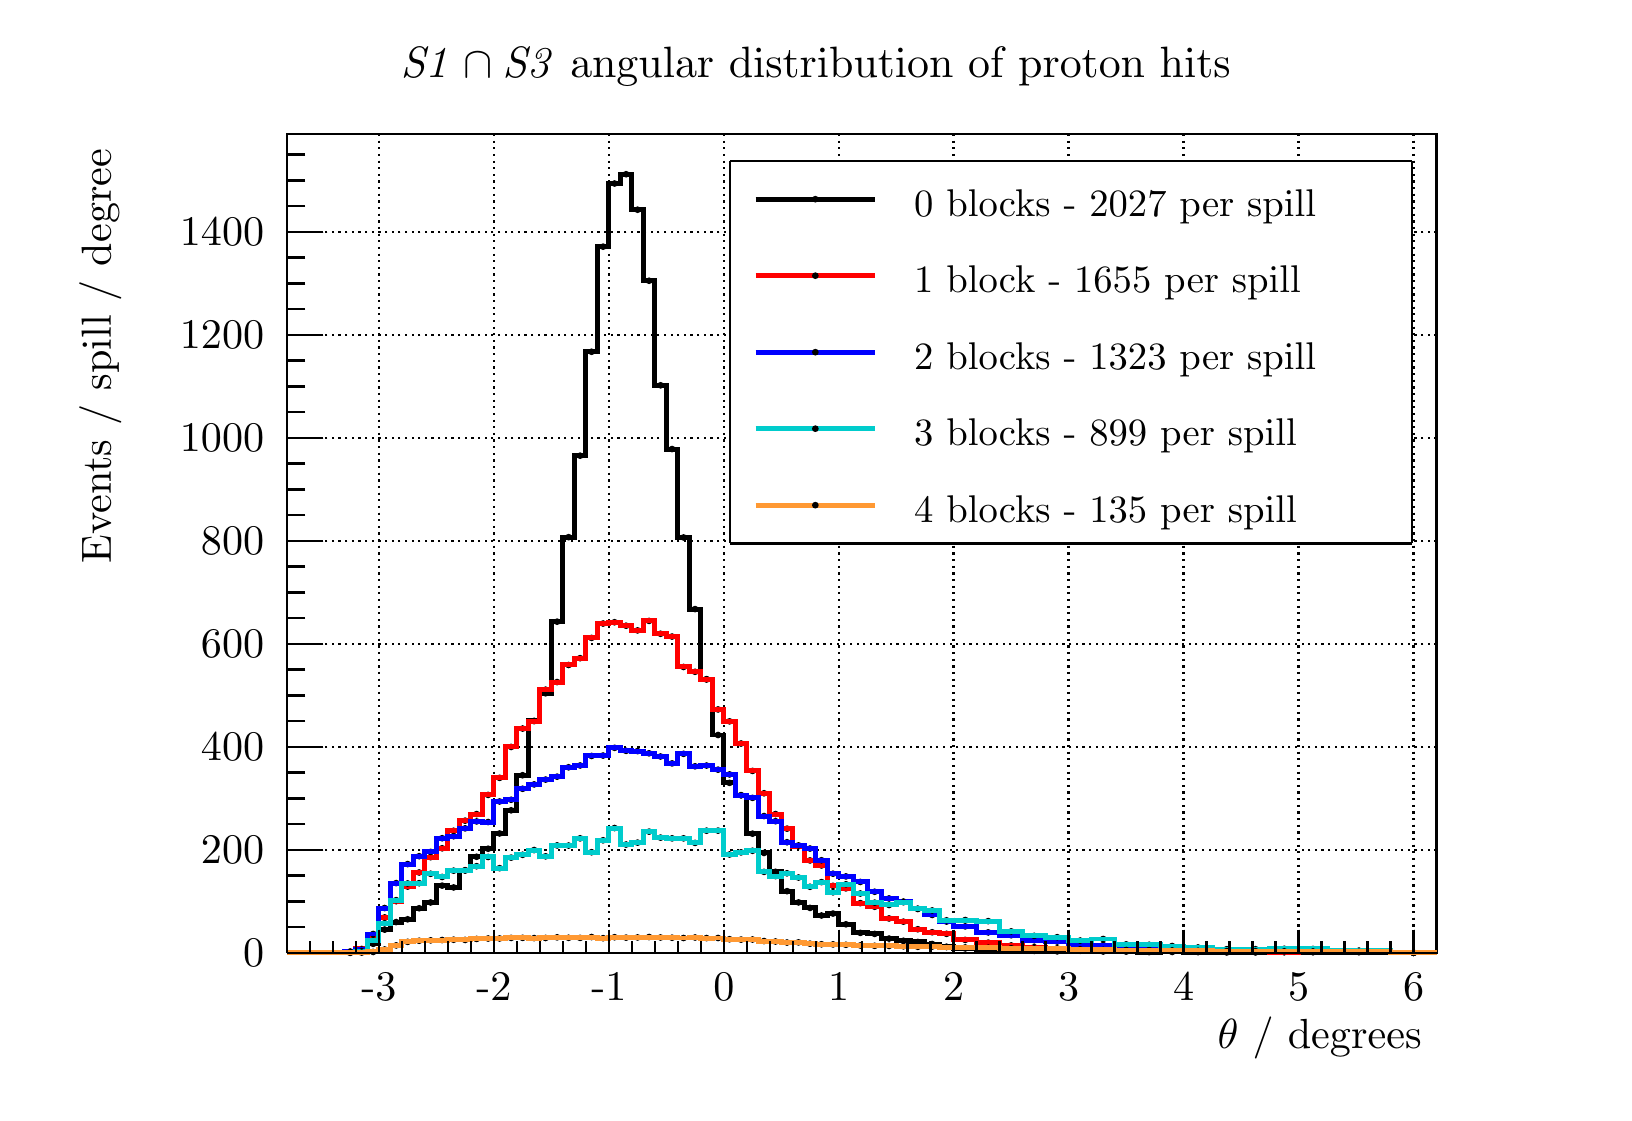
\begin{tikzpicture}
\pgfdeclareplotmark{cross} {
\pgfpathmoveto{\pgfpoint{-0.3\pgfplotmarksize}{\pgfplotmarksize}}
\pgfpathlineto{\pgfpoint{+0.3\pgfplotmarksize}{\pgfplotmarksize}}
\pgfpathlineto{\pgfpoint{+0.3\pgfplotmarksize}{0.3\pgfplotmarksize}}
\pgfpathlineto{\pgfpoint{+1\pgfplotmarksize}{0.3\pgfplotmarksize}}
\pgfpathlineto{\pgfpoint{+1\pgfplotmarksize}{-0.3\pgfplotmarksize}}
\pgfpathlineto{\pgfpoint{+0.3\pgfplotmarksize}{-0.3\pgfplotmarksize}}
\pgfpathlineto{\pgfpoint{+0.3\pgfplotmarksize}{-1.\pgfplotmarksize}}
\pgfpathlineto{\pgfpoint{-0.3\pgfplotmarksize}{-1.\pgfplotmarksize}}
\pgfpathlineto{\pgfpoint{-0.3\pgfplotmarksize}{-0.3\pgfplotmarksize}}
\pgfpathlineto{\pgfpoint{-1.\pgfplotmarksize}{-0.3\pgfplotmarksize}}
\pgfpathlineto{\pgfpoint{-1.\pgfplotmarksize}{0.3\pgfplotmarksize}}
\pgfpathlineto{\pgfpoint{-0.3\pgfplotmarksize}{0.3\pgfplotmarksize}}
\pgfpathclose
\pgfusepathqstroke
}
\pgfdeclareplotmark{cross*} {
\pgfpathmoveto{\pgfpoint{-0.3\pgfplotmarksize}{\pgfplotmarksize}}
\pgfpathlineto{\pgfpoint{+0.3\pgfplotmarksize}{\pgfplotmarksize}}
\pgfpathlineto{\pgfpoint{+0.3\pgfplotmarksize}{0.3\pgfplotmarksize}}
\pgfpathlineto{\pgfpoint{+1\pgfplotmarksize}{0.3\pgfplotmarksize}}
\pgfpathlineto{\pgfpoint{+1\pgfplotmarksize}{-0.3\pgfplotmarksize}}
\pgfpathlineto{\pgfpoint{+0.3\pgfplotmarksize}{-0.3\pgfplotmarksize}}
\pgfpathlineto{\pgfpoint{+0.3\pgfplotmarksize}{-1.\pgfplotmarksize}}
\pgfpathlineto{\pgfpoint{-0.3\pgfplotmarksize}{-1.\pgfplotmarksize}}
\pgfpathlineto{\pgfpoint{-0.3\pgfplotmarksize}{-0.3\pgfplotmarksize}}
\pgfpathlineto{\pgfpoint{-1.\pgfplotmarksize}{-0.3\pgfplotmarksize}}
\pgfpathlineto{\pgfpoint{-1.\pgfplotmarksize}{0.3\pgfplotmarksize}}
\pgfpathlineto{\pgfpoint{-0.3\pgfplotmarksize}{0.3\pgfplotmarksize}}
\pgfpathclose
\pgfusepathqfillstroke
}
\pgfdeclareplotmark{newstar} {
\pgfpathmoveto{\pgfqpoint{0pt}{\pgfplotmarksize}}
\pgfpathlineto{\pgfqpointpolar{44}{0.5\pgfplotmarksize}}
\pgfpathlineto{\pgfqpointpolar{18}{\pgfplotmarksize}}
\pgfpathlineto{\pgfqpointpolar{-20}{0.5\pgfplotmarksize}}
\pgfpathlineto{\pgfqpointpolar{-54}{\pgfplotmarksize}}
\pgfpathlineto{\pgfqpointpolar{-90}{0.5\pgfplotmarksize}}
\pgfpathlineto{\pgfqpointpolar{234}{\pgfplotmarksize}}
\pgfpathlineto{\pgfqpointpolar{198}{0.5\pgfplotmarksize}}
\pgfpathlineto{\pgfqpointpolar{162}{\pgfplotmarksize}}
\pgfpathlineto{\pgfqpointpolar{134}{0.5\pgfplotmarksize}}
\pgfpathclose
\pgfusepathqstroke
}
\pgfdeclareplotmark{newstar*} {
\pgfpathmoveto{\pgfqpoint{0pt}{\pgfplotmarksize}}
\pgfpathlineto{\pgfqpointpolar{44}{0.5\pgfplotmarksize}}
\pgfpathlineto{\pgfqpointpolar{18}{\pgfplotmarksize}}
\pgfpathlineto{\pgfqpointpolar{-20}{0.5\pgfplotmarksize}}
\pgfpathlineto{\pgfqpointpolar{-54}{\pgfplotmarksize}}
\pgfpathlineto{\pgfqpointpolar{-90}{0.5\pgfplotmarksize}}
\pgfpathlineto{\pgfqpointpolar{234}{\pgfplotmarksize}}
\pgfpathlineto{\pgfqpointpolar{198}{0.5\pgfplotmarksize}}
\pgfpathlineto{\pgfqpointpolar{162}{\pgfplotmarksize}}
\pgfpathlineto{\pgfqpointpolar{134}{0.5\pgfplotmarksize}}
\pgfpathclose
\pgfusepathqfillstroke
}
\definecolor{c}{rgb}{1,1,1};
\draw [color=c, fill=c] (0,0) rectangle (20,13.5143);
\draw [color=c, fill=c] (3.28571,1.77143) rectangle (17.8857,12.1714);
\definecolor{c}{rgb}{0,0,0};
\draw [c,line width=0.9] (3.28571,1.77143) -- (3.28571,12.1714) -- (17.8857,12.1714) -- (17.8857,1.77143) -- (3.28571,1.77143);
\definecolor{c}{rgb}{1,1,1};
\draw [color=c, fill=c] (3.28571,1.77143) rectangle (17.8857,12.1714);
\definecolor{c}{rgb}{0,0,0};
\draw [c,line width=0.9] (3.28571,1.77143) -- (3.28571,12.1714) -- (17.8857,12.1714) -- (17.8857,1.77143) -- (3.28571,1.77143);
\draw [c,line width=0.9] (3.28571,1.77143) -- (17.8857,1.77143);
\draw [c,dash pattern=on 0.80pt off 1.60pt ,line width=0.9] (4.45371,12.1714) -- (4.45371,1.77143);
\draw [c,dash pattern=on 0.80pt off 1.60pt ,line width=0.9] (5.91371,12.1714) -- (5.91371,1.77143);
\draw [c,dash pattern=on 0.80pt off 1.60pt ,line width=0.9] (7.37371,12.1714) -- (7.37371,1.77143);
\draw [c,dash pattern=on 0.80pt off 1.60pt ,line width=0.9] (8.83371,12.1714) -- (8.83371,1.77143);
\draw [c,dash pattern=on 0.80pt off 1.60pt ,line width=0.9] (10.2937,12.1714) -- (10.2937,1.77143);
\draw [c,dash pattern=on 0.80pt off 1.60pt ,line width=0.9] (11.7537,12.1714) -- (11.7537,1.77143);
\draw [c,dash pattern=on 0.80pt off 1.60pt ,line width=0.9] (13.2137,12.1714) -- (13.2137,1.77143);
\draw [c,dash pattern=on 0.80pt off 1.60pt ,line width=0.9] (14.6737,12.1714) -- (14.6737,1.77143);
\draw [c,dash pattern=on 0.80pt off 1.60pt ,line width=0.9] (16.1337,12.1714) -- (16.1337,1.77143);
\draw [c,dash pattern=on 0.80pt off 1.60pt ,line width=0.9] (17.5937,12.1714) -- (17.5937,1.77143);
\draw [c,dash pattern=on 0.80pt off 1.60pt ,line width=0.9] (4.45371,12.1714) -- (4.45371,1.77143);
\draw [c,dash pattern=on 0.80pt off 1.60pt ,line width=0.9] (17.5937,12.1714) -- (17.5937,1.77143);
\draw [c,line width=0.9] (3.28571,1.77143) -- (3.28571,12.1714);
\draw [c,dash pattern=on 0.80pt off 1.60pt ,line width=0.9] (17.8857,1.77143) -- (3.28571,1.77143);
\draw [c,dash pattern=on 0.80pt off 1.60pt ,line width=0.9] (17.8857,3.07955) -- (3.28571,3.07955);
\draw [c,dash pattern=on 0.80pt off 1.60pt ,line width=0.9] (17.8857,4.38766) -- (3.28571,4.38766);
\draw [c,dash pattern=on 0.80pt off 1.60pt ,line width=0.9] (17.8857,5.69578) -- (3.28571,5.69578);
\draw [c,dash pattern=on 0.80pt off 1.60pt ,line width=0.9] (17.8857,7.0039) -- (3.28571,7.0039);
\draw [c,dash pattern=on 0.80pt off 1.60pt ,line width=0.9] (17.8857,8.31201) -- (3.28571,8.31201);
\draw [c,dash pattern=on 0.80pt off 1.60pt ,line width=0.9] (17.8857,9.62013) -- (3.28571,9.62013);
\draw [c,dash pattern=on 0.80pt off 1.60pt ,line width=0.9] (17.8857,10.9282) -- (3.28571,10.9282);
\draw [c,dash pattern=on 0.80pt off 1.60pt ,line width=0.9] (17.8857,10.9282) -- (3.28571,10.9282);
\definecolor{c}{rgb}{0,0,0.6};
\draw [c,line width=0.9] (3.28571,1.77143) -- (3.43171,1.77143) -- (3.43171,1.77143) -- (3.57771,1.77143) -- (3.57771,1.77143) -- (3.72371,1.77143) -- (3.72371,1.77143) -- (3.86971,1.77143) -- (3.86971,1.77143) -- (4.01571,1.77143) --
 (4.01571,1.77143) -- (4.16171,1.77143) -- (4.16171,1.77143) -- (4.30771,1.77143) -- (4.30771,1.77143) -- (4.45371,1.77143) -- (4.45371,1.77143) -- (4.59971,1.77143) -- (4.59971,1.77143) -- (4.74571,1.77143) -- (4.74571,1.77143) -- (4.89171,1.77143)
 -- (4.89171,1.77143) -- (5.03771,1.77143) -- (5.03771,1.77143) -- (5.18371,1.77143) -- (5.18371,1.77143) -- (5.32971,1.77143) -- (5.32971,1.77143) -- (5.47571,1.77143) -- (5.47571,1.77143) -- (5.62171,1.77143) -- (5.62171,1.77143) --
 (5.76771,1.77143) -- (5.76771,1.77143) -- (5.91371,1.77143) -- (5.91371,1.77143) -- (6.05971,1.77143) -- (6.05971,1.77143) -- (6.20571,1.77143) -- (6.20571,1.77143) -- (6.35171,1.77143) -- (6.35171,1.77143) -- (6.49771,1.77143) -- (6.49771,1.77143)
 -- (6.64371,1.77143) -- (6.64371,1.77143) -- (6.78971,1.77143) -- (6.78971,1.77143) -- (6.93571,1.77143) -- (6.93571,1.77143) -- (7.08171,1.77143) -- (7.08171,1.77143) -- (7.22771,1.77143) -- (7.22771,1.77143) -- (7.37371,1.77143) --
 (7.37371,1.77143) -- (7.51971,1.77143) -- (7.51971,1.77143) -- (7.66571,1.77143) -- (7.66571,1.77143) -- (7.81171,1.77143) -- (7.81171,1.77143) -- (7.95771,1.77143) -- (7.95771,1.77143) -- (8.10371,1.77143) -- (8.10371,1.77143) -- (8.24971,1.77143)
 -- (8.24971,1.77143) -- (8.39571,1.77143) -- (8.39571,1.77143) -- (8.54171,1.77143) -- (8.54171,1.77143) -- (8.68771,1.77143) -- (8.68771,1.77143) -- (8.83371,1.77143) -- (8.83371,1.77143) -- (8.97971,1.77143) -- (8.97971,1.77143) --
 (9.12571,1.77143) -- (9.12571,1.77143) -- (9.27171,1.77143) -- (9.27171,1.77143) -- (9.41771,1.77143) -- (9.41771,1.77143) -- (9.56371,1.77143) -- (9.56371,1.77143) -- (9.70971,1.77143) -- (9.70971,1.77143) -- (9.85571,1.77143) -- (9.85571,1.77143)
 -- (10.0017,1.77143) -- (10.0017,1.77143) -- (10.1477,1.77143) -- (10.1477,1.77143) -- (10.2937,1.77143) -- (10.2937,1.77143) -- (10.4762,1.77143) -- (10.4762,1.77143) -- (10.6587,1.77143) -- (10.6587,1.77143) -- (10.8412,1.77143) --
 (10.8412,1.77143) -- (11.0237,1.77143) -- (11.0237,1.77143) -- (11.2062,1.77143) -- (11.2062,1.77143) -- (11.3887,1.77143) -- (11.3887,1.77143) -- (11.5712,1.77143) -- (11.5712,1.77143) -- (11.7537,1.77143) -- (11.7537,1.77143) -- (12.0457,1.77143)
 -- (12.0457,1.77143) -- (12.3377,1.77143) -- (12.3377,1.77143) -- (12.6297,1.77143) -- (12.6297,1.77143) -- (12.9217,1.77143) -- (12.9217,1.77143) -- (13.2137,1.77143) -- (13.2137,1.77143) -- (13.5057,1.77143) -- (13.5057,1.77143) --
 (13.7977,1.77143) -- (13.7977,1.77143) -- (14.0897,1.77143) -- (14.0897,1.77143) -- (14.3817,1.77143) -- (14.3817,1.77143) -- (14.6737,1.77143) -- (14.6737,1.77143) -- (15.0387,1.77143) -- (15.0387,1.77143) -- (15.4037,1.77143) -- (15.4037,1.77143)
 -- (15.7687,1.77143) -- (15.7687,1.77143) -- (16.1337,1.77143) -- (16.1337,1.77143) -- (16.4987,1.77143) -- (16.4987,1.77143) -- (17.3017,1.77143) -- (17.3017,1.77143) -- (17.8857,1.77143);
\definecolor{c}{rgb}{0,0,0};
\draw [c,line width=0.9] (3.28571,1.77143) -- (17.8857,1.77143);
\draw [c,line width=0.9] (4.45371,2.06739) -- (4.45371,1.77143);
\draw [c,line width=0.9] (4.74571,1.91941) -- (4.74571,1.77143);
\draw [c,line width=0.9] (5.03771,1.91941) -- (5.03771,1.77143);
\draw [c,line width=0.9] (5.32971,1.91941) -- (5.32971,1.77143);
\draw [c,line width=0.9] (5.62171,1.91941) -- (5.62171,1.77143);
\draw [c,line width=0.9] (5.91371,2.06739) -- (5.91371,1.77143);
\draw [c,line width=0.9] (6.20571,1.91941) -- (6.20571,1.77143);
\draw [c,line width=0.9] (6.49771,1.91941) -- (6.49771,1.77143);
\draw [c,line width=0.9] (6.78971,1.91941) -- (6.78971,1.77143);
\draw [c,line width=0.9] (7.08171,1.91941) -- (7.08171,1.77143);
\draw [c,line width=0.9] (7.37371,2.06739) -- (7.37371,1.77143);
\draw [c,line width=0.9] (7.66571,1.91941) -- (7.66571,1.77143);
\draw [c,line width=0.9] (7.95771,1.91941) -- (7.95771,1.77143);
\draw [c,line width=0.9] (8.24971,1.91941) -- (8.24971,1.77143);
\draw [c,line width=0.9] (8.54171,1.91941) -- (8.54171,1.77143);
\draw [c,line width=0.9] (8.83371,2.06739) -- (8.83371,1.77143);
\draw [c,line width=0.9] (9.12571,1.91941) -- (9.12571,1.77143);
\draw [c,line width=0.9] (9.41771,1.91941) -- (9.41771,1.77143);
\draw [c,line width=0.9] (9.70971,1.91941) -- (9.70971,1.77143);
\draw [c,line width=0.9] (10.0017,1.91941) -- (10.0017,1.77143);
\draw [c,line width=0.9] (10.2937,2.06739) -- (10.2937,1.77143);
\draw [c,line width=0.9] (10.5857,1.91941) -- (10.5857,1.77143);
\draw [c,line width=0.9] (10.8777,1.91941) -- (10.8777,1.77143);
\draw [c,line width=0.9] (11.1697,1.91941) -- (11.1697,1.77143);
\draw [c,line width=0.9] (11.4617,1.91941) -- (11.4617,1.77143);
\draw [c,line width=0.9] (11.7537,2.06739) -- (11.7537,1.77143);
\draw [c,line width=0.9] (12.0457,1.91941) -- (12.0457,1.77143);
\draw [c,line width=0.9] (12.3377,1.91941) -- (12.3377,1.77143);
\draw [c,line width=0.9] (12.6297,1.91941) -- (12.6297,1.77143);
\draw [c,line width=0.9] (12.9217,1.91941) -- (12.9217,1.77143);
\draw [c,line width=0.9] (13.2137,2.06739) -- (13.2137,1.77143);
\draw [c,line width=0.9] (13.5057,1.91941) -- (13.5057,1.77143);
\draw [c,line width=0.9] (13.7977,1.91941) -- (13.7977,1.77143);
\draw [c,line width=0.9] (14.0897,1.91941) -- (14.0897,1.77143);
\draw [c,line width=0.9] (14.3817,1.91941) -- (14.3817,1.77143);
\draw [c,line width=0.9] (14.6737,2.06739) -- (14.6737,1.77143);
\draw [c,line width=0.9] (14.9657,1.91941) -- (14.9657,1.77143);
\draw [c,line width=0.9] (15.2577,1.91941) -- (15.2577,1.77143);
\draw [c,line width=0.9] (15.5497,1.91941) -- (15.5497,1.77143);
\draw [c,line width=0.9] (15.8417,1.91941) -- (15.8417,1.77143);
\draw [c,line width=0.9] (16.1337,2.06739) -- (16.1337,1.77143);
\draw [c,line width=0.9] (16.4257,1.91941) -- (16.4257,1.77143);
\draw [c,line width=0.9] (16.7177,1.91941) -- (16.7177,1.77143);
\draw [c,line width=0.9] (17.0097,1.91941) -- (17.0097,1.77143);
\draw [c,line width=0.9] (17.3017,1.91941) -- (17.3017,1.77143);
\draw [c,line width=0.9] (17.5937,2.06739) -- (17.5937,1.77143);
\draw [c,line width=0.9] (4.45371,2.06739) -- (4.45371,1.77143);
\draw [c,line width=0.9] (4.16171,1.91941) -- (4.16171,1.77143);
\draw [c,line width=0.9] (3.86971,1.91941) -- (3.86971,1.77143);
\draw [c,line width=0.9] (3.57771,1.91941) -- (3.57771,1.77143);
\draw [c,line width=0.9] (17.5937,2.06739) -- (17.5937,1.77143);
\draw [anchor=base] (4.45371,1.16329) node[scale=1.52295, color=c, rotate=0]{-3};
\draw [anchor=base] (5.91371,1.16329) node[scale=1.52295, color=c, rotate=0]{-2};
\draw [anchor=base] (7.37371,1.16329) node[scale=1.52295, color=c, rotate=0]{-1};
\draw [anchor=base] (8.83371,1.16329) node[scale=1.52295, color=c, rotate=0]{0};
\draw [anchor=base] (10.2937,1.16329) node[scale=1.52295, color=c, rotate=0]{1};
\draw [anchor=base] (11.7537,1.16329) node[scale=1.52295, color=c, rotate=0]{2};
\draw [anchor=base] (13.2137,1.16329) node[scale=1.52295, color=c, rotate=0]{3};
\draw [anchor=base] (14.6737,1.16329) node[scale=1.52295, color=c, rotate=0]{4};
\draw [anchor=base] (16.1337,1.16329) node[scale=1.52295, color=c, rotate=0]{5};
\draw [anchor=base] (17.5937,1.16329) node[scale=1.52295, color=c, rotate=0]{6};
\draw [anchor= east] (17.8857,0.690286) node[scale=1.52295, color=c, rotate=0]{$\theta$ / degrees};
\draw [c,line width=0.9] (3.28571,1.77143) -- (3.28571,12.1714);
\draw [c,line width=0.9] (3.74745,1.77143) -- (3.28571,1.77143);
\draw [c,line width=0.9] (3.51658,2.09846) -- (3.28571,2.09846);
\draw [c,line width=0.9] (3.51658,2.42549) -- (3.28571,2.42549);
\draw [c,line width=0.9] (3.51658,2.75252) -- (3.28571,2.75252);
\draw [c,line width=0.9] (3.74745,3.07955) -- (3.28571,3.07955);
\draw [c,line width=0.9] (3.51658,3.40658) -- (3.28571,3.40658);
\draw [c,line width=0.9] (3.51658,3.7336) -- (3.28571,3.7336);
\draw [c,line width=0.9] (3.51658,4.06063) -- (3.28571,4.06063);
\draw [c,line width=0.9] (3.74745,4.38766) -- (3.28571,4.38766);
\draw [c,line width=0.9] (3.51658,4.71469) -- (3.28571,4.71469);
\draw [c,line width=0.9] (3.51658,5.04172) -- (3.28571,5.04172);
\draw [c,line width=0.9] (3.51658,5.36875) -- (3.28571,5.36875);
\draw [c,line width=0.9] (3.74745,5.69578) -- (3.28571,5.69578);
\draw [c,line width=0.9] (3.51658,6.02281) -- (3.28571,6.02281);
\draw [c,line width=0.9] (3.51658,6.34984) -- (3.28571,6.34984);
\draw [c,line width=0.9] (3.51658,6.67687) -- (3.28571,6.67687);
\draw [c,line width=0.9] (3.74745,7.0039) -- (3.28571,7.0039);
\draw [c,line width=0.9] (3.51658,7.33093) -- (3.28571,7.33093);
\draw [c,line width=0.9] (3.51658,7.65796) -- (3.28571,7.65796);
\draw [c,line width=0.9] (3.51658,7.98499) -- (3.28571,7.98499);
\draw [c,line width=0.9] (3.74745,8.31201) -- (3.28571,8.31201);
\draw [c,line width=0.9] (3.51658,8.63904) -- (3.28571,8.63904);
\draw [c,line width=0.9] (3.51658,8.96607) -- (3.28571,8.96607);
\draw [c,line width=0.9] (3.51658,9.2931) -- (3.28571,9.2931);
\draw [c,line width=0.9] (3.74745,9.62013) -- (3.28571,9.62013);
\draw [c,line width=0.9] (3.51658,9.94716) -- (3.28571,9.94716);
\draw [c,line width=0.9] (3.51658,10.2742) -- (3.28571,10.2742);
\draw [c,line width=0.9] (3.51658,10.6012) -- (3.28571,10.6012);
\draw [c,line width=0.9] (3.74745,10.9282) -- (3.28571,10.9282);
\draw [c,line width=0.9] (3.74745,10.9282) -- (3.28571,10.9282);
\draw [c,line width=0.9] (3.51658,11.2553) -- (3.28571,11.2553);
\draw [c,line width=0.9] (3.51658,11.5823) -- (3.28571,11.5823);
\draw [c,line width=0.9] (3.51658,11.9093) -- (3.28571,11.9093);
\draw [anchor= east] (3.18571,1.77143) node[scale=1.52295, color=c, rotate=0]{0};
\draw [anchor= east] (3.18571,3.07955) node[scale=1.52295, color=c, rotate=0]{200};
\draw [anchor= east] (3.18571,4.38766) node[scale=1.52295, color=c, rotate=0]{400};
\draw [anchor= east] (3.18571,5.69578) node[scale=1.52295, color=c, rotate=0]{600};
\draw [anchor= east] (3.18571,7.0039) node[scale=1.52295, color=c, rotate=0]{800};
\draw [anchor= east] (3.18571,8.31201) node[scale=1.52295, color=c, rotate=0]{1000};
\draw [anchor= east] (3.18571,9.62013) node[scale=1.52295, color=c, rotate=0]{1200};
\draw [anchor= east] (3.18571,10.9282) node[scale=1.52295, color=c, rotate=0]{1400};
\draw [anchor= east] (0.914286,12.1714) node[scale=1.52295, color=c, rotate=90]{ Events / spill / degree};
\draw [c,line width=1.8] (4.08871,1.77928) -- (4.08871,1.77976);
\draw [c,line width=1.8] (4.08871,1.77976) -- (4.08871,1.78025);
\foreach \P in {(4.08871,1.77976)}{\draw[mark options={color=c,fill=c},mark size=2.402402pt,mark=*,mark size=1pt] plot coordinates {\P};}
\draw [c,line width=1.8] (4.23471,1.80702) -- (4.23471,1.808);
\draw [c,line width=1.8] (4.23471,1.808) -- (4.23471,1.80898);
\foreach \P in {(4.23471,1.808)}{\draw[mark options={color=c,fill=c},mark size=2.402402pt,mark=*,mark size=1pt] plot coordinates {\P};}
\draw [c,line width=1.8] (4.38071,1.88391) -- (4.38071,1.88565);
\draw [c,line width=1.8] (4.38071,1.88565) -- (4.38071,1.88738);
\foreach \P in {(4.38071,1.88565)}{\draw[mark options={color=c,fill=c},mark size=2.402402pt,mark=*,mark size=1pt] plot coordinates {\P};}
\draw [c,line width=1.8] (4.52671,2.0637) -- (4.52671,2.0665);
\draw [c,line width=1.8] (4.52671,2.0665) -- (4.52671,2.0693);
\foreach \P in {(4.52671,2.0665)}{\draw[mark options={color=c,fill=c},mark size=2.402402pt,mark=*,mark size=1pt] plot coordinates {\P};}
\draw [c,line width=1.8] (4.67271,2.15927) -- (4.67271,2.16245);
\draw [c,line width=1.8] (4.67271,2.16245) -- (4.67271,2.16564);
\foreach \P in {(4.67271,2.16245)}{\draw[mark options={color=c,fill=c},mark size=2.402402pt,mark=*,mark size=1pt] plot coordinates {\P};}
\draw [c,line width=1.8] (4.81871,2.19429) -- (4.81871,2.19763);
\draw [c,line width=1.8] (4.81871,2.19763) -- (4.81871,2.20096);
\foreach \P in {(4.81871,2.19763)}{\draw[mark options={color=c,fill=c},mark size=2.402402pt,mark=*,mark size=1pt] plot coordinates {\P};}
\draw [c,line width=1.8] (4.96471,2.33421) -- (4.96471,2.33808);
\draw [c,line width=1.8] (4.96471,2.33808) -- (4.96471,2.34194);
\foreach \P in {(4.96471,2.33808)}{\draw[mark options={color=c,fill=c},mark size=2.402402pt,mark=*,mark size=1pt] plot coordinates {\P};}
\draw [c,line width=1.8] (5.11071,2.40725) -- (5.11071,2.41137);
\draw [c,line width=1.8] (5.11071,2.41137) -- (5.11071,2.41549);
\foreach \P in {(5.11071,2.41137)}{\draw[mark options={color=c,fill=c},mark size=2.402402pt,mark=*,mark size=1pt] plot coordinates {\P};}
\draw [c,line width=1.8] (5.25671,2.62065) -- (5.25671,2.62539);
\draw [c,line width=1.8] (5.25671,2.62539) -- (5.25671,2.63013);
\foreach \P in {(5.25671,2.62539)}{\draw[mark options={color=c,fill=c},mark size=2.402402pt,mark=*,mark size=1pt] plot coordinates {\P};}
\draw [c,line width=1.8] (5.40271,2.5977) -- (5.40271,2.60239);
\draw [c,line width=1.8] (5.40271,2.60239) -- (5.40271,2.60707);
\foreach \P in {(5.40271,2.60239)}{\draw[mark options={color=c,fill=c},mark size=2.402402pt,mark=*,mark size=1pt] plot coordinates {\P};}
\draw [c,line width=1.8] (5.54871,2.8114) -- (5.54871,2.81666);
\draw [c,line width=1.8] (5.54871,2.81666) -- (5.54871,2.82192);
\foreach \P in {(5.54871,2.81666)}{\draw[mark options={color=c,fill=c},mark size=2.402402pt,mark=*,mark size=1pt] plot coordinates {\P};}
\draw [c,line width=1.8] (5.69471,2.9861) -- (5.69471,2.99178);
\draw [c,line width=1.8] (5.69471,2.99178) -- (5.69471,2.99746);
\foreach \P in {(5.69471,2.99178)}{\draw[mark options={color=c,fill=c},mark size=2.402402pt,mark=*,mark size=1pt] plot coordinates {\P};}
\draw [c,line width=1.8] (5.84071,3.08772) -- (5.84071,3.09363);
\draw [c,line width=1.8] (5.84071,3.09363) -- (5.84071,3.09954);
\foreach \P in {(5.84071,3.09363)}{\draw[mark options={color=c,fill=c},mark size=2.402402pt,mark=*,mark size=1pt] plot coordinates {\P};}
\draw [c,line width=1.8] (5.98671,3.28119) -- (5.98671,3.28753);
\draw [c,line width=1.8] (5.98671,3.28753) -- (5.98671,3.29387);
\foreach \P in {(5.98671,3.28753)}{\draw[mark options={color=c,fill=c},mark size=2.402402pt,mark=*,mark size=1pt] plot coordinates {\P};}
\draw [c,line width=1.8] (6.13271,3.57494) -- (6.13271,3.58187);
\draw [c,line width=1.8] (6.13271,3.58187) -- (6.13271,3.58879);
\foreach \P in {(6.13271,3.58187)}{\draw[mark options={color=c,fill=c},mark size=2.402402pt,mark=*,mark size=1pt] plot coordinates {\P};}
\draw [c,line width=1.8] (6.27871,4.01937) -- (6.27871,4.02712);
\draw [c,line width=1.8] (6.27871,4.02712) -- (6.27871,4.03486);
\foreach \P in {(6.27871,4.02712)}{\draw[mark options={color=c,fill=c},mark size=2.402402pt,mark=*,mark size=1pt] plot coordinates {\P};}
\draw [c,line width=1.8] (6.42471,4.70892) -- (6.42471,4.71772);
\draw [c,line width=1.8] (6.42471,4.71772) -- (6.42471,4.72652);
\foreach \P in {(6.42471,4.71772)}{\draw[mark options={color=c,fill=c},mark size=2.402402pt,mark=*,mark size=1pt] plot coordinates {\P};}
\draw [c,line width=1.8] (6.57071,5.05873) -- (6.57071,5.06808);
\draw [c,line width=1.8] (6.57071,5.06808) -- (6.57071,5.07743);
\foreach \P in {(6.57071,5.06808)}{\draw[mark options={color=c,fill=c},mark size=2.402402pt,mark=*,mark size=1pt] plot coordinates {\P};}
\draw [c,line width=1.8] (6.71671,5.96677) -- (6.71671,5.9773);
\draw [c,line width=1.8] (6.71671,5.9773) -- (6.71671,5.98784);
\foreach \P in {(6.71671,5.9773)}{\draw[mark options={color=c,fill=c},mark size=2.402402pt,mark=*,mark size=1pt] plot coordinates {\P};}
\draw [c,line width=1.8] (6.86271,7.03879) -- (6.86271,7.05058);
\draw [c,line width=1.8] (6.86271,7.05058) -- (6.86271,7.06238);
\foreach \P in {(6.86271,7.05058)}{\draw[mark options={color=c,fill=c},mark size=2.402402pt,mark=*,mark size=1pt] plot coordinates {\P};}
\draw [c,line width=1.8] (7.00871,8.07255) -- (7.00871,8.08548);
\draw [c,line width=1.8] (7.00871,8.08548) -- (7.00871,8.09841);
\foreach \P in {(7.00871,8.08548)}{\draw[mark options={color=c,fill=c},mark size=2.402402pt,mark=*,mark size=1pt] plot coordinates {\P};}
\draw [c,line width=1.8] (7.15471,9.39111) -- (7.15471,9.40531);
\draw [c,line width=1.8] (7.15471,9.40531) -- (7.15471,9.41952);
\foreach \P in {(7.15471,9.40531)}{\draw[mark options={color=c,fill=c},mark size=2.402402pt,mark=*,mark size=1pt] plot coordinates {\P};}
\draw [c,line width=1.8] (7.30071,10.7244) -- (7.30071,10.7398);
\draw [c,line width=1.8] (7.30071,10.7398) -- (7.30071,10.7552);
\foreach \P in {(7.30071,10.7398)}{\draw[mark options={color=c,fill=c},mark size=2.402402pt,mark=*,mark size=1pt] plot coordinates {\P};}
\draw [c,line width=1.8] (7.44671,11.5259) -- (7.44671,11.542);
\draw [c,line width=1.8] (7.44671,11.542) -- (7.44671,11.5581);
\foreach \P in {(7.44671,11.542)}{\draw[mark options={color=c,fill=c},mark size=2.402402pt,mark=*,mark size=1pt] plot coordinates {\P};}
\draw [c,line width=1.8] (7.59271,11.6439) -- (7.59271,11.66);
\draw [c,line width=1.8] (7.59271,11.66) -- (7.59271,11.6762);
\foreach \P in {(7.59271,11.66)}{\draw[mark options={color=c,fill=c},mark size=2.402402pt,mark=*,mark size=1pt] plot coordinates {\P};}
\draw [c,line width=1.8] (7.73871,11.1933) -- (7.73871,11.2091);
\draw [c,line width=1.8] (7.73871,11.2091) -- (7.73871,11.2249);
\foreach \P in {(7.73871,11.2091)}{\draw[mark options={color=c,fill=c},mark size=2.402402pt,mark=*,mark size=1pt] plot coordinates {\P};}
\draw [c,line width=1.8] (7.88471,10.292) -- (7.88471,10.307);
\draw [c,line width=1.8] (7.88471,10.307) -- (7.88471,10.322);
\foreach \P in {(7.88471,10.307)}{\draw[mark options={color=c,fill=c},mark size=2.402402pt,mark=*,mark size=1pt] plot coordinates {\P};}
\draw [c,line width=1.8] (8.03071,8.96539) -- (8.03071,8.97916);
\draw [c,line width=1.8] (8.03071,8.97916) -- (8.03071,8.99293);
\foreach \P in {(8.03071,8.97916)}{\draw[mark options={color=c,fill=c},mark size=2.402402pt,mark=*,mark size=1pt] plot coordinates {\P};}
\draw [c,line width=1.8] (8.17671,8.15671) -- (8.17671,8.1697);
\draw [c,line width=1.8] (8.17671,8.1697) -- (8.17671,8.18269);
\foreach \P in {(8.17671,8.1697)}{\draw[mark options={color=c,fill=c},mark size=2.402402pt,mark=*,mark size=1pt] plot coordinates {\P};}
\draw [c,line width=1.8] (8.32271,7.03519) -- (8.32271,7.04698);
\draw [c,line width=1.8] (8.32271,7.04698) -- (8.32271,7.05876);
\foreach \P in {(8.32271,7.04698)}{\draw[mark options={color=c,fill=c},mark size=2.402402pt,mark=*,mark size=1pt] plot coordinates {\P};}
\draw [c,line width=1.8] (8.46871,6.12634) -- (8.46871,6.13709);
\draw [c,line width=1.8] (8.46871,6.13709) -- (8.46871,6.14784);
\foreach \P in {(8.46871,6.13709)}{\draw[mark options={color=c,fill=c},mark size=2.402402pt,mark=*,mark size=1pt] plot coordinates {\P};}
\draw [c,line width=1.8] (8.61471,5.23363) -- (8.61471,5.24318);
\draw [c,line width=1.8] (8.61471,5.24318) -- (8.61471,5.25272);
\foreach \P in {(8.61471,5.24318)}{\draw[mark options={color=c,fill=c},mark size=2.402402pt,mark=*,mark size=1pt] plot coordinates {\P};}
\draw [c,line width=1.8] (8.76071,4.52978) -- (8.76071,4.53832);
\draw [c,line width=1.8] (8.76071,4.53832) -- (8.76071,4.54686);
\foreach \P in {(8.76071,4.53832)}{\draw[mark options={color=c,fill=c},mark size=2.402402pt,mark=*,mark size=1pt] plot coordinates {\P};}
\draw [c,line width=1.8] (8.90671,3.9228) -- (8.90671,3.93034);
\draw [c,line width=1.8] (8.90671,3.93034) -- (8.90671,3.93787);
\foreach \P in {(8.90671,3.93034)}{\draw[mark options={color=c,fill=c},mark size=2.402402pt,mark=*,mark size=1pt] plot coordinates {\P};}
\draw [c,line width=1.8] (9.05271,3.76622) -- (9.05271,3.77346);
\draw [c,line width=1.8] (9.05271,3.77346) -- (9.05271,3.7807);
\foreach \P in {(9.05271,3.77346)}{\draw[mark options={color=c,fill=c},mark size=2.402402pt,mark=*,mark size=1pt] plot coordinates {\P};}
\draw [c,line width=1.8] (9.19871,3.27871) -- (9.19871,3.28503);
\draw [c,line width=1.8] (9.19871,3.28503) -- (9.19871,3.29134);
\foreach \P in {(9.19871,3.28503)}{\draw[mark options={color=c,fill=c},mark size=2.402402pt,mark=*,mark size=1pt] plot coordinates {\P};}
\draw [c,line width=1.8] (9.34471,3.0343) -- (9.34471,3.0401);
\draw [c,line width=1.8] (9.34471,3.0401) -- (9.34471,3.04591);
\foreach \P in {(9.34471,3.0401)}{\draw[mark options={color=c,fill=c},mark size=2.402402pt,mark=*,mark size=1pt] plot coordinates {\P};}
\draw [c,line width=1.8] (9.49071,2.7953) -- (9.49071,2.8005);
\draw [c,line width=1.8] (9.49071,2.8005) -- (9.49071,2.8057);
\foreach \P in {(9.49071,2.8005)}{\draw[mark options={color=c,fill=c},mark size=2.402402pt,mark=*,mark size=1pt] plot coordinates {\P};}
\draw [c,line width=1.8] (9.63671,2.55056) -- (9.63671,2.55512);
\draw [c,line width=1.8] (9.63671,2.55512) -- (9.63671,2.55967);
\foreach \P in {(9.63671,2.55512)}{\draw[mark options={color=c,fill=c},mark size=2.402402pt,mark=*,mark size=1pt] plot coordinates {\P};}
\draw [c,line width=1.8] (9.78271,2.40811) -- (9.78271,2.41224);
\draw [c,line width=1.8] (9.78271,2.41224) -- (9.78271,2.41636);
\foreach \P in {(9.78271,2.41224)}{\draw[mark options={color=c,fill=c},mark size=2.402402pt,mark=*,mark size=1pt] plot coordinates {\P};}
\draw [c,line width=1.8] (9.92871,2.33856) -- (9.92871,2.34245);
\draw [c,line width=1.8] (9.92871,2.34245) -- (9.92871,2.34633);
\foreach \P in {(9.92871,2.34245)}{\draw[mark options={color=c,fill=c},mark size=2.402402pt,mark=*,mark size=1pt] plot coordinates {\P};}
\draw [c,line width=1.8] (10.0747,2.24253) -- (10.0747,2.24605);
\draw [c,line width=1.8] (10.0747,2.24605) -- (10.0747,2.24957);
\foreach \P in {(10.0747,2.24605)}{\draw[mark options={color=c,fill=c},mark size=2.402402pt,mark=*,mark size=1pt] plot coordinates {\P};}
\draw [c,line width=1.8] (10.2207,2.26683) -- (10.2207,2.27048);
\draw [c,line width=1.8] (10.2207,2.27048) -- (10.2207,2.27413);
\foreach \P in {(10.2207,2.27048)}{\draw[mark options={color=c,fill=c},mark size=2.402402pt,mark=*,mark size=1pt] plot coordinates {\P};}
\draw [c,line width=1.8] (10.385,2.13071) -- (10.385,2.13417);
\draw [c,line width=1.8] (10.385,2.13417) -- (10.385,2.13762);
\foreach \P in {(10.385,2.13417)}{\draw[mark options={color=c,fill=c},mark size=2.402402pt,mark=*,mark size=1pt] plot coordinates {\P};}
\draw [c,line width=1.8] (10.5675,2.0223) -- (10.5675,2.02518);
\draw [c,line width=1.8] (10.5675,2.02518) -- (10.5675,2.02807);
\foreach \P in {(10.5675,2.02518)}{\draw[mark options={color=c,fill=c},mark size=2.402402pt,mark=*,mark size=1pt] plot coordinates {\P};}
\draw [c,line width=1.8] (10.75,2.0093) -- (10.75,2.01214);
\draw [c,line width=1.8] (10.75,2.01214) -- (10.75,2.01497);
\foreach \P in {(10.75,2.01214)}{\draw[mark options={color=c,fill=c},mark size=2.402402pt,mark=*,mark size=1pt] plot coordinates {\P};}
\draw [c,line width=1.8] (10.9325,1.95041) -- (10.9325,1.95285);
\draw [c,line width=1.8] (10.9325,1.95285) -- (10.9325,1.95529);
\foreach \P in {(10.9325,1.95285)}{\draw[mark options={color=c,fill=c},mark size=2.402402pt,mark=*,mark size=1pt] plot coordinates {\P};}
\draw [c,line width=1.8] (11.115,1.92247) -- (11.115,1.92473);
\draw [c,line width=1.8] (11.115,1.92473) -- (11.115,1.92699);
\foreach \P in {(11.115,1.92473)}{\draw[mark options={color=c,fill=c},mark size=2.402402pt,mark=*,mark size=1pt] plot coordinates {\P};}
\draw [c,line width=1.8] (11.2975,1.90792) -- (11.2975,1.91006);
\draw [c,line width=1.8] (11.2975,1.91006) -- (11.2975,1.9122);
\foreach \P in {(11.2975,1.91006)}{\draw[mark options={color=c,fill=c},mark size=2.402402pt,mark=*,mark size=1pt] plot coordinates {\P};}
\draw [c,line width=1.8] (11.48,1.88169) -- (11.48,1.88362);
\draw [c,line width=1.8] (11.48,1.88362) -- (11.48,1.88556);
\foreach \P in {(11.48,1.88362)}{\draw[mark options={color=c,fill=c},mark size=2.402402pt,mark=*,mark size=1pt] plot coordinates {\P};}
\draw [c,line width=1.8] (11.6625,1.84719) -- (11.6625,1.84877);
\draw [c,line width=1.8] (11.6625,1.84877) -- (11.6625,1.85034);
\foreach \P in {(11.6625,1.84877)}{\draw[mark options={color=c,fill=c},mark size=2.402402pt,mark=*,mark size=1pt] plot coordinates {\P};}
\draw [c,line width=1.8] (11.8997,1.8255) -- (11.8997,1.82722);
\draw [c,line width=1.8] (11.8997,1.82722) -- (11.8997,1.82893);
\foreach \P in {(11.8997,1.82722)}{\draw[mark options={color=c,fill=c},mark size=2.402402pt,mark=*,mark size=1pt] plot coordinates {\P};}
\draw [c,line width=1.8] (12.1917,1.80911) -- (12.1917,1.81054);
\draw [c,line width=1.8] (12.1917,1.81054) -- (12.1917,1.81198);
\foreach \P in {(12.1917,1.81054)}{\draw[mark options={color=c,fill=c},mark size=2.402402pt,mark=*,mark size=1pt] plot coordinates {\P};}
\draw [c,line width=1.8] (12.4837,1.80809) -- (12.4837,1.80951);
\draw [c,line width=1.8] (12.4837,1.80951) -- (12.4837,1.81093);
\foreach \P in {(12.4837,1.80951)}{\draw[mark options={color=c,fill=c},mark size=2.402402pt,mark=*,mark size=1pt] plot coordinates {\P};}
\draw [c,line width=1.8] (12.7757,1.79522) -- (12.7757,1.79637);
\draw [c,line width=1.8] (12.7757,1.79637) -- (12.7757,1.79753);
\foreach \P in {(12.7757,1.79637)}{\draw[mark options={color=c,fill=c},mark size=2.402402pt,mark=*,mark size=1pt] plot coordinates {\P};}
\draw [c,line width=1.8] (13.0677,1.78926) -- (13.0677,1.79027);
\draw [c,line width=1.8] (13.0677,1.79027) -- (13.0677,1.79128);
\foreach \P in {(13.0677,1.79027)}{\draw[mark options={color=c,fill=c},mark size=2.402402pt,mark=*,mark size=1pt] plot coordinates {\P};}
\draw [c,line width=1.8] (13.3597,1.7964) -- (13.3597,1.79758);
\draw [c,line width=1.8] (13.3597,1.79758) -- (13.3597,1.79876);
\foreach \P in {(13.3597,1.79758)}{\draw[mark options={color=c,fill=c},mark size=2.402402pt,mark=*,mark size=1pt] plot coordinates {\P};}
\draw [c,line width=1.8] (13.6517,1.78712) -- (13.6517,1.78804);
\draw [c,line width=1.8] (13.6517,1.78804) -- (13.6517,1.78897);
\foreach \P in {(13.6517,1.78804)}{\draw[mark options={color=c,fill=c},mark size=2.402402pt,mark=*,mark size=1pt] plot coordinates {\P};}
\draw [c,line width=1.8] (13.9437,1.78641) -- (13.9437,1.78733);
\draw [c,line width=1.8] (13.9437,1.78733) -- (13.9437,1.78826);
\foreach \P in {(13.9437,1.78733)}{\draw[mark options={color=c,fill=c},mark size=2.402402pt,mark=*,mark size=1pt] plot coordinates {\P};}
\draw [c,line width=1.8] (14.2357,1.78046) -- (14.2357,1.7812);
\draw [c,line width=1.8] (14.2357,1.7812) -- (14.2357,1.78194);
\foreach \P in {(14.2357,1.7812)}{\draw[mark options={color=c,fill=c},mark size=2.402402pt,mark=*,mark size=1pt] plot coordinates {\P};}
\draw [c,line width=1.8] (14.5277,1.78232) -- (14.5277,1.7831);
\draw [c,line width=1.8] (14.5277,1.7831) -- (14.5277,1.78389);
\foreach \P in {(14.5277,1.7831)}{\draw[mark options={color=c,fill=c},mark size=2.402402pt,mark=*,mark size=1pt] plot coordinates {\P};}
\draw [c,line width=1.8] (14.8562,1.77979) -- (14.8562,1.78055);
\draw [c,line width=1.8] (14.8562,1.78055) -- (14.8562,1.78132);
\foreach \P in {(14.8562,1.78055)}{\draw[mark options={color=c,fill=c},mark size=2.402402pt,mark=*,mark size=1pt] plot coordinates {\P};}
\draw [c,line width=1.8] (15.2212,1.77593) -- (15.2212,1.7765);
\draw [c,line width=1.8] (15.2212,1.7765) -- (15.2212,1.77707);
\foreach \P in {(15.2212,1.7765)}{\draw[mark options={color=c,fill=c},mark size=2.402402pt,mark=*,mark size=1pt] plot coordinates {\P};}
\draw [c,line width=1.8] (15.5862,1.77596) -- (15.5862,1.77653);
\draw [c,line width=1.8] (15.5862,1.77653) -- (15.5862,1.7771);
\foreach \P in {(15.5862,1.77653)}{\draw[mark options={color=c,fill=c},mark size=2.402402pt,mark=*,mark size=1pt] plot coordinates {\P};}
\draw [c,line width=1.8] (15.9512,1.77912) -- (15.9512,1.77987);
\draw [c,line width=1.8] (15.9512,1.77987) -- (15.9512,1.78062);
\foreach \P in {(15.9512,1.77987)}{\draw[mark options={color=c,fill=c},mark size=2.402402pt,mark=*,mark size=1pt] plot coordinates {\P};}
\draw [c,line width=1.8] (16.3162,1.77848) -- (16.3162,1.77922);
\draw [c,line width=1.8] (16.3162,1.77922) -- (16.3162,1.77995);
\foreach \P in {(16.3162,1.77922)}{\draw[mark options={color=c,fill=c},mark size=2.402402pt,mark=*,mark size=1pt] plot coordinates {\P};}
\draw [c,line width=1.8] (16.9002,1.77875) -- (16.9002,1.77985);
\draw [c,line width=1.8] (16.9002,1.77985) -- (16.9002,1.78094);
\foreach \P in {(16.9002,1.77985)}{\draw[mark options={color=c,fill=c},mark size=2.402402pt,mark=*,mark size=1pt] plot coordinates {\P};}
\draw [c,line width=1.8] (17.5937,1.77212) -- (17.5937,1.77269);
\draw [c,line width=1.8] (17.5937,1.77269) -- (17.5937,1.77325);
\foreach \P in {(17.5937,1.77269)}{\draw[mark options={color=c,fill=c},mark size=2.402402pt,mark=*,mark size=1pt] plot coordinates {\P};}
\draw [c,line width=1.8] (3.28571,1.77143) -- (3.43171,1.77143) -- (3.43171,1.77143) -- (3.57771,1.77143) -- (3.57771,1.77143) -- (3.72371,1.77143) -- (3.72371,1.77143) -- (3.86971,1.77143) -- (3.86971,1.77143) -- (4.01571,1.77143) --
 (4.01571,1.77976) -- (4.16171,1.77976) -- (4.16171,1.808) -- (4.30771,1.808) -- (4.30771,1.88565) -- (4.45371,1.88565) -- (4.45371,2.0665) -- (4.59971,2.0665) -- (4.59971,2.16245) -- (4.74571,2.16245) -- (4.74571,2.19763) -- (4.89171,2.19763) --
 (4.89171,2.33808) -- (5.03771,2.33808) -- (5.03771,2.41137) -- (5.18371,2.41137) -- (5.18371,2.62539) -- (5.32971,2.62539) -- (5.32971,2.60239) -- (5.47571,2.60239) -- (5.47571,2.81666) -- (5.62171,2.81666) -- (5.62171,2.99178) -- (5.76771,2.99178)
 -- (5.76771,3.09363) -- (5.91371,3.09363) -- (5.91371,3.28753) -- (6.05971,3.28753) -- (6.05971,3.58187) -- (6.20571,3.58187) -- (6.20571,4.02712) -- (6.35171,4.02712) -- (6.35171,4.71772) -- (6.49771,4.71772) -- (6.49771,5.06808) --
 (6.64371,5.06808) -- (6.64371,5.9773) -- (6.78971,5.9773) -- (6.78971,7.05058) -- (6.93571,7.05058) -- (6.93571,8.08548) -- (7.08171,8.08548) -- (7.08171,9.40531) -- (7.22771,9.40531) -- (7.22771,10.7398) -- (7.37371,10.7398) -- (7.37371,11.542) --
 (7.51971,11.542) -- (7.51971,11.66) -- (7.66571,11.66) -- (7.66571,11.2091) -- (7.81171,11.2091) -- (7.81171,10.307) -- (7.95771,10.307) -- (7.95771,8.97916) -- (8.10371,8.97916) -- (8.10371,8.1697) -- (8.24971,8.1697) -- (8.24971,7.04698) --
 (8.39571,7.04698) -- (8.39571,6.13709) -- (8.54171,6.13709) -- (8.54171,5.24318) -- (8.68771,5.24318) -- (8.68771,4.53832) -- (8.83371,4.53832) -- (8.83371,3.93034) -- (8.97971,3.93034) -- (8.97971,3.77346) -- (9.12571,3.77346) -- (9.12571,3.28503)
 -- (9.27171,3.28503) -- (9.27171,3.0401) -- (9.41771,3.0401) -- (9.41771,2.8005) -- (9.56371,2.8005) -- (9.56371,2.55512) -- (9.70971,2.55512) -- (9.70971,2.41224) -- (9.85571,2.41224) -- (9.85571,2.34245) -- (10.0017,2.34245) -- (10.0017,2.24605)
 -- (10.1477,2.24605) -- (10.1477,2.27048) -- (10.2937,2.27048) -- (10.2937,2.13417) -- (10.4762,2.13417) -- (10.4762,2.02518) -- (10.6587,2.02518) -- (10.6587,2.01214) -- (10.8412,2.01214) -- (10.8412,1.95285) -- (11.0237,1.95285) --
 (11.0237,1.92473) -- (11.2062,1.92473) -- (11.2062,1.91006) -- (11.3887,1.91006) -- (11.3887,1.88362) -- (11.5712,1.88362) -- (11.5712,1.84877) -- (11.7537,1.84877) -- (11.7537,1.82722) -- (12.0457,1.82722) -- (12.0457,1.81054) -- (12.3377,1.81054)
 -- (12.3377,1.80951) -- (12.6297,1.80951) -- (12.6297,1.79637) -- (12.9217,1.79637) -- (12.9217,1.79027) -- (13.2137,1.79027) -- (13.2137,1.79758) -- (13.5057,1.79758) -- (13.5057,1.78804) -- (13.7977,1.78804) -- (13.7977,1.78733) --
 (14.0897,1.78733) -- (14.0897,1.7812) -- (14.3817,1.7812) -- (14.3817,1.7831) -- (14.6737,1.7831) -- (14.6737,1.78055) -- (15.0387,1.78055) -- (15.0387,1.7765) -- (15.4037,1.7765) -- (15.4037,1.77653) -- (15.7687,1.77653) -- (15.7687,1.77987) --
 (16.1337,1.77987) -- (16.1337,1.77922) -- (16.4987,1.77922) -- (16.4987,1.77985) -- (17.3017,1.77985) -- (17.3017,1.77269) -- (17.8857,1.77269);
\definecolor{c}{rgb}{1,0,0};
\draw [c,line width=1.8] (4.08871,1.77445) -- (4.08871,1.77469);
\draw [c,line width=1.8] (4.08871,1.77469) -- (4.08871,1.77492);
\definecolor{c}{rgb}{0,0,0};
\foreach \P in {(4.08871,1.77469)}{\draw[mark options={color=c,fill=c},mark size=2.402402pt,mark=*,mark size=1pt] plot coordinates {\P};}
\definecolor{c}{rgb}{1,0,0};
\draw [c,line width=1.8] (4.23471,1.82002) -- (4.23471,1.82097);
\draw [c,line width=1.8] (4.23471,1.82097) -- (4.23471,1.82192);
\definecolor{c}{rgb}{0,0,0};
\foreach \P in {(4.23471,1.82097)}{\draw[mark options={color=c,fill=c},mark size=2.402402pt,mark=*,mark size=1pt] plot coordinates {\P};}
\definecolor{c}{rgb}{1,0,0};
\draw [c,line width=1.8] (4.38071,1.96606) -- (4.38071,1.96794);
\draw [c,line width=1.8] (4.38071,1.96794) -- (4.38071,1.96981);
\definecolor{c}{rgb}{0,0,0};
\foreach \P in {(4.38071,1.96794)}{\draw[mark options={color=c,fill=c},mark size=2.402402pt,mark=*,mark size=1pt] plot coordinates {\P};}
\definecolor{c}{rgb}{1,0,0};
\draw [c,line width=1.8] (4.52671,2.21881) -- (4.52671,2.22166);
\draw [c,line width=1.8] (4.52671,2.22166) -- (4.52671,2.22452);
\definecolor{c}{rgb}{0,0,0};
\foreach \P in {(4.52671,2.22166)}{\draw[mark options={color=c,fill=c},mark size=2.402402pt,mark=*,mark size=1pt] plot coordinates {\P};}
\definecolor{c}{rgb}{1,0,0};
\draw [c,line width=1.8] (4.67271,2.4243) -- (4.67271,2.42776);
\draw [c,line width=1.8] (4.67271,2.42776) -- (4.67271,2.43122);
\definecolor{c}{rgb}{0,0,0};
\foreach \P in {(4.67271,2.42776)}{\draw[mark options={color=c,fill=c},mark size=2.402402pt,mark=*,mark size=1pt] plot coordinates {\P};}
\definecolor{c}{rgb}{1,0,0};
\draw [c,line width=1.8] (4.81871,2.60907) -- (4.81871,2.61297);
\draw [c,line width=1.8] (4.81871,2.61297) -- (4.81871,2.61687);
\definecolor{c}{rgb}{0,0,0};
\foreach \P in {(4.81871,2.61297)}{\draw[mark options={color=c,fill=c},mark size=2.402402pt,mark=*,mark size=1pt] plot coordinates {\P};}
\definecolor{c}{rgb}{1,0,0};
\draw [c,line width=1.8] (4.96471,2.78794) -- (4.96471,2.79225);
\draw [c,line width=1.8] (4.96471,2.79225) -- (4.96471,2.79656);
\definecolor{c}{rgb}{0,0,0};
\foreach \P in {(4.96471,2.79225)}{\draw[mark options={color=c,fill=c},mark size=2.402402pt,mark=*,mark size=1pt] plot coordinates {\P};}
\definecolor{c}{rgb}{1,0,0};
\draw [c,line width=1.8] (5.11071,2.98186) -- (5.11071,2.98652);
\draw [c,line width=1.8] (5.11071,2.98652) -- (5.11071,2.99119);
\definecolor{c}{rgb}{0,0,0};
\foreach \P in {(5.11071,2.98652)}{\draw[mark options={color=c,fill=c},mark size=2.402402pt,mark=*,mark size=1pt] plot coordinates {\P};}
\definecolor{c}{rgb}{1,0,0};
\draw [c,line width=1.8] (5.25671,3.0946) -- (5.25671,3.09948);
\draw [c,line width=1.8] (5.25671,3.09948) -- (5.25671,3.10435);
\definecolor{c}{rgb}{0,0,0};
\foreach \P in {(5.25671,3.09948)}{\draw[mark options={color=c,fill=c},mark size=2.402402pt,mark=*,mark size=1pt] plot coordinates {\P};}
\definecolor{c}{rgb}{1,0,0};
\draw [c,line width=1.8] (5.40271,3.31671) -- (5.40271,3.32202);
\draw [c,line width=1.8] (5.40271,3.32202) -- (5.40271,3.32733);
\definecolor{c}{rgb}{0,0,0};
\foreach \P in {(5.40271,3.32202)}{\draw[mark options={color=c,fill=c},mark size=2.402402pt,mark=*,mark size=1pt] plot coordinates {\P};}
\definecolor{c}{rgb}{1,0,0};
\draw [c,line width=1.8] (5.54871,3.44465) -- (5.54871,3.45014);
\draw [c,line width=1.8] (5.54871,3.45014) -- (5.54871,3.45564);
\definecolor{c}{rgb}{0,0,0};
\foreach \P in {(5.54871,3.45014)}{\draw[mark options={color=c,fill=c},mark size=2.402402pt,mark=*,mark size=1pt] plot coordinates {\P};}
\definecolor{c}{rgb}{1,0,0};
\draw [c,line width=1.8] (5.69471,3.52805) -- (5.69471,3.53371);
\draw [c,line width=1.8] (5.69471,3.53371) -- (5.69471,3.53938);
\definecolor{c}{rgb}{0,0,0};
\foreach \P in {(5.69471,3.53371)}{\draw[mark options={color=c,fill=c},mark size=2.402402pt,mark=*,mark size=1pt] plot coordinates {\P};}
\definecolor{c}{rgb}{1,0,0};
\draw [c,line width=1.8] (5.84071,3.77145) -- (5.84071,3.77748);
\draw [c,line width=1.8] (5.84071,3.77748) -- (5.84071,3.78352);
\definecolor{c}{rgb}{0,0,0};
\foreach \P in {(5.84071,3.77748)}{\draw[mark options={color=c,fill=c},mark size=2.402402pt,mark=*,mark size=1pt] plot coordinates {\P};}
\definecolor{c}{rgb}{1,0,0};
\draw [c,line width=1.8] (5.98671,3.98767) -- (5.98671,3.99399);
\draw [c,line width=1.8] (5.98671,3.99399) -- (5.98671,4.00031);
\definecolor{c}{rgb}{0,0,0};
\foreach \P in {(5.98671,3.99399)}{\draw[mark options={color=c,fill=c},mark size=2.402402pt,mark=*,mark size=1pt] plot coordinates {\P};}
\definecolor{c}{rgb}{1,0,0};
\draw [c,line width=1.8] (6.13271,4.37974) -- (6.13271,4.38659);
\draw [c,line width=1.8] (6.13271,4.38659) -- (6.13271,4.39345);
\definecolor{c}{rgb}{0,0,0};
\foreach \P in {(6.13271,4.38659)}{\draw[mark options={color=c,fill=c},mark size=2.402402pt,mark=*,mark size=1pt] plot coordinates {\P};}
\definecolor{c}{rgb}{1,0,0};
\draw [c,line width=1.8] (6.27871,4.61285) -- (6.27871,4.62002);
\draw [c,line width=1.8] (6.27871,4.62002) -- (6.27871,4.62718);
\definecolor{c}{rgb}{0,0,0};
\foreach \P in {(6.27871,4.62002)}{\draw[mark options={color=c,fill=c},mark size=2.402402pt,mark=*,mark size=1pt] plot coordinates {\P};}
\definecolor{c}{rgb}{1,0,0};
\draw [c,line width=1.8] (6.42471,4.70723) -- (6.42471,4.7145);
\draw [c,line width=1.8] (6.42471,4.7145) -- (6.42471,4.72177);
\definecolor{c}{rgb}{0,0,0};
\foreach \P in {(6.42471,4.7145)}{\draw[mark options={color=c,fill=c},mark size=2.402402pt,mark=*,mark size=1pt] plot coordinates {\P};}
\definecolor{c}{rgb}{1,0,0};
\draw [c,line width=1.8] (6.57071,5.10572) -- (6.57071,5.11349);
\draw [c,line width=1.8] (6.57071,5.11349) -- (6.57071,5.12126);
\definecolor{c}{rgb}{0,0,0};
\foreach \P in {(6.57071,5.11349)}{\draw[mark options={color=c,fill=c},mark size=2.402402pt,mark=*,mark size=1pt] plot coordinates {\P};}
\definecolor{c}{rgb}{1,0,0};
\draw [c,line width=1.8] (6.71671,5.20261) -- (6.71671,5.21048);
\draw [c,line width=1.8] (6.71671,5.21048) -- (6.71671,5.21835);
\definecolor{c}{rgb}{0,0,0};
\foreach \P in {(6.71671,5.21048)}{\draw[mark options={color=c,fill=c},mark size=2.402402pt,mark=*,mark size=1pt] plot coordinates {\P};}
\definecolor{c}{rgb}{1,0,0};
\draw [c,line width=1.8] (6.86271,5.4194) -- (6.86271,5.42752);
\draw [c,line width=1.8] (6.86271,5.42752) -- (6.86271,5.43563);
\definecolor{c}{rgb}{0,0,0};
\foreach \P in {(6.86271,5.42752)}{\draw[mark options={color=c,fill=c},mark size=2.402402pt,mark=*,mark size=1pt] plot coordinates {\P};}
\definecolor{c}{rgb}{1,0,0};
\draw [c,line width=1.8] (7.00871,5.50593) -- (7.00871,5.51417);
\draw [c,line width=1.8] (7.00871,5.51417) -- (7.00871,5.52241);
\definecolor{c}{rgb}{0,0,0};
\foreach \P in {(7.00871,5.51417)}{\draw[mark options={color=c,fill=c},mark size=2.402402pt,mark=*,mark size=1pt] plot coordinates {\P};}
\definecolor{c}{rgb}{1,0,0};
\draw [c,line width=1.8] (7.15471,5.76288) -- (7.15471,5.77137);
\draw [c,line width=1.8] (7.15471,5.77137) -- (7.15471,5.77986);
\definecolor{c}{rgb}{0,0,0};
\foreach \P in {(7.15471,5.77137)}{\draw[mark options={color=c,fill=c},mark size=2.402402pt,mark=*,mark size=1pt] plot coordinates {\P};}
\definecolor{c}{rgb}{1,0,0};
\draw [c,line width=1.8] (7.30071,5.94516) -- (7.30071,5.95384);
\draw [c,line width=1.8] (7.30071,5.95384) -- (7.30071,5.96253);
\definecolor{c}{rgb}{0,0,0};
\foreach \P in {(7.30071,5.95384)}{\draw[mark options={color=c,fill=c},mark size=2.402402pt,mark=*,mark size=1pt] plot coordinates {\P};}
\definecolor{c}{rgb}{1,0,0};
\draw [c,line width=1.8] (7.44671,5.96139) -- (7.44671,5.97013);
\draw [c,line width=1.8] (7.44671,5.97013) -- (7.44671,5.97887);
\definecolor{c}{rgb}{0,0,0};
\foreach \P in {(7.44671,5.97013)}{\draw[mark options={color=c,fill=c},mark size=2.402402pt,mark=*,mark size=1pt] plot coordinates {\P};}
\definecolor{c}{rgb}{1,0,0};
\draw [c,line width=1.8] (7.59271,5.91738) -- (7.59271,5.92604);
\draw [c,line width=1.8] (7.59271,5.92604) -- (7.59271,5.93471);
\definecolor{c}{rgb}{0,0,0};
\foreach \P in {(7.59271,5.92604)}{\draw[mark options={color=c,fill=c},mark size=2.402402pt,mark=*,mark size=1pt] plot coordinates {\P};}
\definecolor{c}{rgb}{1,0,0};
\draw [c,line width=1.8] (7.73871,5.85796) -- (7.73871,5.86656);
\draw [c,line width=1.8] (7.73871,5.86656) -- (7.73871,5.87516);
\definecolor{c}{rgb}{0,0,0};
\foreach \P in {(7.73871,5.86656)}{\draw[mark options={color=c,fill=c},mark size=2.402402pt,mark=*,mark size=1pt] plot coordinates {\P};}
\definecolor{c}{rgb}{1,0,0};
\draw [c,line width=1.8] (7.88471,5.97847) -- (7.88471,5.98721);
\draw [c,line width=1.8] (7.88471,5.98721) -- (7.88471,5.99594);
\definecolor{c}{rgb}{0,0,0};
\foreach \P in {(7.88471,5.98721)}{\draw[mark options={color=c,fill=c},mark size=2.402402pt,mark=*,mark size=1pt] plot coordinates {\P};}
\definecolor{c}{rgb}{1,0,0};
\draw [c,line width=1.8] (8.03071,5.81562) -- (8.03071,5.82417);
\draw [c,line width=1.8] (8.03071,5.82417) -- (8.03071,5.83272);
\definecolor{c}{rgb}{0,0,0};
\foreach \P in {(8.03071,5.82417)}{\draw[mark options={color=c,fill=c},mark size=2.402402pt,mark=*,mark size=1pt] plot coordinates {\P};}
\definecolor{c}{rgb}{1,0,0};
\draw [c,line width=1.8] (8.17671,5.78004) -- (8.17671,5.78858);
\draw [c,line width=1.8] (8.17671,5.78858) -- (8.17671,5.79713);
\definecolor{c}{rgb}{0,0,0};
\foreach \P in {(8.17671,5.78858)}{\draw[mark options={color=c,fill=c},mark size=2.402402pt,mark=*,mark size=1pt] plot coordinates {\P};}
\definecolor{c}{rgb}{1,0,0};
\draw [c,line width=1.8] (8.32271,5.39403) -- (8.32271,5.40211);
\draw [c,line width=1.8] (8.32271,5.40211) -- (8.32271,5.41019);
\definecolor{c}{rgb}{0,0,0};
\foreach \P in {(8.32271,5.40211)}{\draw[mark options={color=c,fill=c},mark size=2.402402pt,mark=*,mark size=1pt] plot coordinates {\P};}
\definecolor{c}{rgb}{1,0,0};
\draw [c,line width=1.8] (8.46871,5.33284) -- (8.46871,5.34089);
\draw [c,line width=1.8] (8.46871,5.34089) -- (8.46871,5.34895);
\definecolor{c}{rgb}{0,0,0};
\foreach \P in {(8.46871,5.34089)}{\draw[mark options={color=c,fill=c},mark size=2.402402pt,mark=*,mark size=1pt] plot coordinates {\P};}
\definecolor{c}{rgb}{1,0,0};
\draw [c,line width=1.8] (8.61471,5.23997) -- (8.61471,5.24791);
\draw [c,line width=1.8] (8.61471,5.24791) -- (8.61471,5.25585);
\definecolor{c}{rgb}{0,0,0};
\foreach \P in {(8.61471,5.24791)}{\draw[mark options={color=c,fill=c},mark size=2.402402pt,mark=*,mark size=1pt] plot coordinates {\P};}
\definecolor{c}{rgb}{1,0,0};
\draw [c,line width=1.8] (8.76071,4.85529) -- (8.76071,4.86275);
\draw [c,line width=1.8] (8.76071,4.86275) -- (8.76071,4.87021);
\definecolor{c}{rgb}{0,0,0};
\foreach \P in {(8.76071,4.86275)}{\draw[mark options={color=c,fill=c},mark size=2.402402pt,mark=*,mark size=1pt] plot coordinates {\P};}
\definecolor{c}{rgb}{1,0,0};
\draw [c,line width=1.8] (8.90671,4.70411) -- (8.90671,4.71142);
\draw [c,line width=1.8] (8.90671,4.71142) -- (8.90671,4.71873);
\definecolor{c}{rgb}{0,0,0};
\foreach \P in {(8.90671,4.71142)}{\draw[mark options={color=c,fill=c},mark size=2.402402pt,mark=*,mark size=1pt] plot coordinates {\P};}
\definecolor{c}{rgb}{1,0,0};
\draw [c,line width=1.8] (9.05271,4.42322) -- (9.05271,4.43014);
\draw [c,line width=1.8] (9.05271,4.43014) -- (9.05271,4.43705);
\definecolor{c}{rgb}{0,0,0};
\foreach \P in {(9.05271,4.43014)}{\draw[mark options={color=c,fill=c},mark size=2.402402pt,mark=*,mark size=1pt] plot coordinates {\P};}
\definecolor{c}{rgb}{1,0,0};
\draw [c,line width=1.8] (9.19871,4.0759) -- (9.19871,4.08238);
\draw [c,line width=1.8] (9.19871,4.08238) -- (9.19871,4.08886);
\definecolor{c}{rgb}{0,0,0};
\foreach \P in {(9.19871,4.08238)}{\draw[mark options={color=c,fill=c},mark size=2.402402pt,mark=*,mark size=1pt] plot coordinates {\P};}
\definecolor{c}{rgb}{1,0,0};
\draw [c,line width=1.8] (9.34471,3.79231) -- (9.34471,3.79836);
\draw [c,line width=1.8] (9.34471,3.79836) -- (9.34471,3.80442);
\definecolor{c}{rgb}{0,0,0};
\foreach \P in {(9.34471,3.79836)}{\draw[mark options={color=c,fill=c},mark size=2.402402pt,mark=*,mark size=1pt] plot coordinates {\P};}
\definecolor{c}{rgb}{1,0,0};
\draw [c,line width=1.8] (9.49071,3.52856) -- (9.49071,3.53421);
\draw [c,line width=1.8] (9.49071,3.53421) -- (9.49071,3.53986);
\definecolor{c}{rgb}{0,0,0};
\foreach \P in {(9.49071,3.53421)}{\draw[mark options={color=c,fill=c},mark size=2.402402pt,mark=*,mark size=1pt] plot coordinates {\P};}
\definecolor{c}{rgb}{1,0,0};
\draw [c,line width=1.8] (9.63671,3.34363) -- (9.63671,3.34892);
\draw [c,line width=1.8] (9.63671,3.34892) -- (9.63671,3.35421);
\definecolor{c}{rgb}{0,0,0};
\foreach \P in {(9.63671,3.34892)}{\draw[mark options={color=c,fill=c},mark size=2.402402pt,mark=*,mark size=1pt] plot coordinates {\P};}
\definecolor{c}{rgb}{1,0,0};
\draw [c,line width=1.8] (9.78271,3.12103) -- (9.78271,3.12597);
\draw [c,line width=1.8] (9.78271,3.12597) -- (9.78271,3.13092);
\definecolor{c}{rgb}{0,0,0};
\foreach \P in {(9.78271,3.12597)}{\draw[mark options={color=c,fill=c},mark size=2.402402pt,mark=*,mark size=1pt] plot coordinates {\P};}
\definecolor{c}{rgb}{1,0,0};
\draw [c,line width=1.8] (9.92871,2.94059) -- (9.92871,2.94519);
\draw [c,line width=1.8] (9.92871,2.94519) -- (9.92871,2.94979);
\definecolor{c}{rgb}{0,0,0};
\foreach \P in {(9.92871,2.94519)}{\draw[mark options={color=c,fill=c},mark size=2.402402pt,mark=*,mark size=1pt] plot coordinates {\P};}
\definecolor{c}{rgb}{1,0,0};
\draw [c,line width=1.8] (10.0747,2.87689) -- (10.0747,2.88137);
\draw [c,line width=1.8] (10.0747,2.88137) -- (10.0747,2.88584);
\definecolor{c}{rgb}{0,0,0};
\foreach \P in {(10.0747,2.88137)}{\draw[mark options={color=c,fill=c},mark size=2.402402pt,mark=*,mark size=1pt] plot coordinates {\P};}
\definecolor{c}{rgb}{1,0,0};
\draw [c,line width=1.8] (10.2207,2.61888) -- (10.2207,2.62281);
\draw [c,line width=1.8] (10.2207,2.62281) -- (10.2207,2.62674);
\definecolor{c}{rgb}{0,0,0};
\foreach \P in {(10.2207,2.62281)}{\draw[mark options={color=c,fill=c},mark size=2.402402pt,mark=*,mark size=1pt] plot coordinates {\P};}
\definecolor{c}{rgb}{1,0,0};
\draw [c,line width=1.8] (10.385,2.58642) -- (10.385,2.59075);
\draw [c,line width=1.8] (10.385,2.59075) -- (10.385,2.59509);
\definecolor{c}{rgb}{0,0,0};
\foreach \P in {(10.385,2.59075)}{\draw[mark options={color=c,fill=c},mark size=2.402402pt,mark=*,mark size=1pt] plot coordinates {\P};}
\definecolor{c}{rgb}{1,0,0};
\draw [c,line width=1.8] (10.5675,2.39922) -- (10.5675,2.403);
\draw [c,line width=1.8] (10.5675,2.403) -- (10.5675,2.40678);
\definecolor{c}{rgb}{0,0,0};
\foreach \P in {(10.5675,2.403)}{\draw[mark options={color=c,fill=c},mark size=2.402402pt,mark=*,mark size=1pt] plot coordinates {\P};}
\definecolor{c}{rgb}{1,0,0};
\draw [c,line width=1.8] (10.75,2.35336) -- (10.75,2.357);
\draw [c,line width=1.8] (10.75,2.357) -- (10.75,2.36063);
\definecolor{c}{rgb}{0,0,0};
\foreach \P in {(10.75,2.357)}{\draw[mark options={color=c,fill=c},mark size=2.402402pt,mark=*,mark size=1pt] plot coordinates {\P};}
\definecolor{c}{rgb}{1,0,0};
\draw [c,line width=1.8] (10.9325,2.20542) -- (10.9325,2.20855);
\draw [c,line width=1.8] (10.9325,2.20855) -- (10.9325,2.21168);
\definecolor{c}{rgb}{0,0,0};
\foreach \P in {(10.9325,2.20855)}{\draw[mark options={color=c,fill=c},mark size=2.402402pt,mark=*,mark size=1pt] plot coordinates {\P};}
\definecolor{c}{rgb}{1,0,0};
\draw [c,line width=1.8] (11.115,2.16495) -- (11.115,2.16794);
\draw [c,line width=1.8] (11.115,2.16794) -- (11.115,2.17093);
\definecolor{c}{rgb}{0,0,0};
\foreach \P in {(11.115,2.16794)}{\draw[mark options={color=c,fill=c},mark size=2.402402pt,mark=*,mark size=1pt] plot coordinates {\P};}
\definecolor{c}{rgb}{1,0,0};
\draw [c,line width=1.8] (11.2975,2.06864) -- (11.2975,2.07122);
\draw [c,line width=1.8] (11.2975,2.07122) -- (11.2975,2.0738);
\definecolor{c}{rgb}{0,0,0};
\foreach \P in {(11.2975,2.07122)}{\draw[mark options={color=c,fill=c},mark size=2.402402pt,mark=*,mark size=1pt] plot coordinates {\P};}
\definecolor{c}{rgb}{1,0,0};
\draw [c,line width=1.8] (11.48,2.03057) -- (11.48,2.03303);
\draw [c,line width=1.8] (11.48,2.03303) -- (11.48,2.03548);
\definecolor{c}{rgb}{0,0,0};
\foreach \P in {(11.48,2.03303)}{\draw[mark options={color=c,fill=c},mark size=2.402402pt,mark=*,mark size=1pt] plot coordinates {\P};}
\definecolor{c}{rgb}{1,0,0};
\draw [c,line width=1.8] (11.6625,2.01073) -- (11.6625,2.01307);
\draw [c,line width=1.8] (11.6625,2.01307) -- (11.6625,2.01541);
\definecolor{c}{rgb}{0,0,0};
\foreach \P in {(11.6625,2.01307)}{\draw[mark options={color=c,fill=c},mark size=2.402402pt,mark=*,mark size=1pt] plot coordinates {\P};}
\definecolor{c}{rgb}{1,0,0};
\draw [c,line width=1.8] (11.8997,1.93359) -- (11.8997,1.93603);
\draw [c,line width=1.8] (11.8997,1.93603) -- (11.8997,1.93846);
\definecolor{c}{rgb}{0,0,0};
\foreach \P in {(11.8997,1.93603)}{\draw[mark options={color=c,fill=c},mark size=2.402402pt,mark=*,mark size=1pt] plot coordinates {\P};}
\definecolor{c}{rgb}{1,0,0};
\draw [c,line width=1.8] (12.1917,1.8985) -- (12.1917,1.90064);
\draw [c,line width=1.8] (12.1917,1.90064) -- (12.1917,1.90277);
\definecolor{c}{rgb}{0,0,0};
\foreach \P in {(12.1917,1.90064)}{\draw[mark options={color=c,fill=c},mark size=2.402402pt,mark=*,mark size=1pt] plot coordinates {\P};}
\definecolor{c}{rgb}{1,0,0};
\draw [c,line width=1.8] (12.4837,1.8639) -- (12.4837,1.86573);
\draw [c,line width=1.8] (12.4837,1.86573) -- (12.4837,1.86757);
\definecolor{c}{rgb}{0,0,0};
\foreach \P in {(12.4837,1.86573)}{\draw[mark options={color=c,fill=c},mark size=2.402402pt,mark=*,mark size=1pt] plot coordinates {\P};}
\definecolor{c}{rgb}{1,0,0};
\draw [c,line width=1.8] (12.7757,1.84211) -- (12.7757,1.84372);
\draw [c,line width=1.8] (12.7757,1.84372) -- (12.7757,1.84533);
\definecolor{c}{rgb}{0,0,0};
\foreach \P in {(12.7757,1.84372)}{\draw[mark options={color=c,fill=c},mark size=2.402402pt,mark=*,mark size=1pt] plot coordinates {\P};}
\definecolor{c}{rgb}{1,0,0};
\draw [c,line width=1.8] (13.0677,1.82739) -- (13.0677,1.82884);
\draw [c,line width=1.8] (13.0677,1.82884) -- (13.0677,1.83028);
\definecolor{c}{rgb}{0,0,0};
\foreach \P in {(13.0677,1.82884)}{\draw[mark options={color=c,fill=c},mark size=2.402402pt,mark=*,mark size=1pt] plot coordinates {\P};}
\definecolor{c}{rgb}{1,0,0};
\draw [c,line width=1.8] (13.3597,1.8236) -- (13.3597,1.82498);
\draw [c,line width=1.8] (13.3597,1.82498) -- (13.3597,1.82636);
\definecolor{c}{rgb}{0,0,0};
\foreach \P in {(13.3597,1.82498)}{\draw[mark options={color=c,fill=c},mark size=2.402402pt,mark=*,mark size=1pt] plot coordinates {\P};}
\definecolor{c}{rgb}{1,0,0};
\draw [c,line width=1.8] (13.6517,1.80079) -- (13.6517,1.80183);
\draw [c,line width=1.8] (13.6517,1.80183) -- (13.6517,1.80287);
\definecolor{c}{rgb}{0,0,0};
\foreach \P in {(13.6517,1.80183)}{\draw[mark options={color=c,fill=c},mark size=2.402402pt,mark=*,mark size=1pt] plot coordinates {\P};}
\definecolor{c}{rgb}{1,0,0};
\draw [c,line width=1.8] (13.9437,1.7968) -- (13.9437,1.79776);
\draw [c,line width=1.8] (13.9437,1.79776) -- (13.9437,1.79872);
\definecolor{c}{rgb}{0,0,0};
\foreach \P in {(13.9437,1.79776)}{\draw[mark options={color=c,fill=c},mark size=2.402402pt,mark=*,mark size=1pt] plot coordinates {\P};}
\definecolor{c}{rgb}{1,0,0};
\draw [c,line width=1.8] (14.2357,1.79622) -- (14.2357,1.79717);
\draw [c,line width=1.8] (14.2357,1.79717) -- (14.2357,1.79812);
\definecolor{c}{rgb}{0,0,0};
\foreach \P in {(14.2357,1.79717)}{\draw[mark options={color=c,fill=c},mark size=2.402402pt,mark=*,mark size=1pt] plot coordinates {\P};}
\definecolor{c}{rgb}{1,0,0};
\draw [c,line width=1.8] (14.5277,1.79267) -- (14.5277,1.79355);
\draw [c,line width=1.8] (14.5277,1.79355) -- (14.5277,1.79443);
\definecolor{c}{rgb}{0,0,0};
\foreach \P in {(14.5277,1.79355)}{\draw[mark options={color=c,fill=c},mark size=2.402402pt,mark=*,mark size=1pt] plot coordinates {\P};}
\definecolor{c}{rgb}{1,0,0};
\draw [c,line width=1.8] (14.8562,1.78942) -- (14.8562,1.79037);
\draw [c,line width=1.8] (14.8562,1.79037) -- (14.8562,1.79132);
\definecolor{c}{rgb}{0,0,0};
\foreach \P in {(14.8562,1.79037)}{\draw[mark options={color=c,fill=c},mark size=2.402402pt,mark=*,mark size=1pt] plot coordinates {\P};}
\definecolor{c}{rgb}{1,0,0};
\draw [c,line width=1.8] (15.2212,1.7871) -- (15.2212,1.78798);
\draw [c,line width=1.8] (15.2212,1.78798) -- (15.2212,1.78885);
\definecolor{c}{rgb}{0,0,0};
\foreach \P in {(15.2212,1.78798)}{\draw[mark options={color=c,fill=c},mark size=2.402402pt,mark=*,mark size=1pt] plot coordinates {\P};}
\definecolor{c}{rgb}{1,0,0};
\draw [c,line width=1.8] (15.5862,1.78809) -- (15.5862,1.78897);
\draw [c,line width=1.8] (15.5862,1.78897) -- (15.5862,1.78986);
\definecolor{c}{rgb}{0,0,0};
\foreach \P in {(15.5862,1.78897)}{\draw[mark options={color=c,fill=c},mark size=2.402402pt,mark=*,mark size=1pt] plot coordinates {\P};}
\definecolor{c}{rgb}{1,0,0};
\draw [c,line width=1.8] (15.9512,1.78129) -- (15.9512,1.78196);
\draw [c,line width=1.8] (15.9512,1.78196) -- (15.9512,1.78263);
\definecolor{c}{rgb}{0,0,0};
\foreach \P in {(15.9512,1.78196)}{\draw[mark options={color=c,fill=c},mark size=2.402402pt,mark=*,mark size=1pt] plot coordinates {\P};}
\definecolor{c}{rgb}{1,0,0};
\draw [c,line width=1.8] (16.3162,1.78948) -- (16.3162,1.7904);
\draw [c,line width=1.8] (16.3162,1.7904) -- (16.3162,1.79132);
\definecolor{c}{rgb}{0,0,0};
\foreach \P in {(16.3162,1.7904)}{\draw[mark options={color=c,fill=c},mark size=2.402402pt,mark=*,mark size=1pt] plot coordinates {\P};}
\definecolor{c}{rgb}{1,0,0};
\draw [c,line width=1.8] (16.9002,1.7864) -- (16.9002,1.78769);
\draw [c,line width=1.8] (16.9002,1.78769) -- (16.9002,1.78898);
\definecolor{c}{rgb}{0,0,0};
\foreach \P in {(16.9002,1.78769)}{\draw[mark options={color=c,fill=c},mark size=2.402402pt,mark=*,mark size=1pt] plot coordinates {\P};}
\definecolor{c}{rgb}{1,0,0};
\draw [c,line width=1.8] (17.5937,1.77278) -- (17.5937,1.77338);
\draw [c,line width=1.8] (17.5937,1.77338) -- (17.5937,1.77398);
\definecolor{c}{rgb}{0,0,0};
\foreach \P in {(17.5937,1.77338)}{\draw[mark options={color=c,fill=c},mark size=2.402402pt,mark=*,mark size=1pt] plot coordinates {\P};}
\definecolor{c}{rgb}{1,0,0};
\draw [c,line width=1.8] (3.28571,1.77143) -- (3.43171,1.77143) -- (3.43171,1.77143) -- (3.57771,1.77143) -- (3.57771,1.77143) -- (3.72371,1.77143) -- (3.72371,1.77143) -- (3.86971,1.77143) -- (3.86971,1.77143) -- (4.01571,1.77143) --
 (4.01571,1.77469) -- (4.16171,1.77469) -- (4.16171,1.82097) -- (4.30771,1.82097) -- (4.30771,1.96794) -- (4.45371,1.96794) -- (4.45371,2.22166) -- (4.59971,2.22166) -- (4.59971,2.42776) -- (4.74571,2.42776) -- (4.74571,2.61297) -- (4.89171,2.61297)
 -- (4.89171,2.79225) -- (5.03771,2.79225) -- (5.03771,2.98652) -- (5.18371,2.98652) -- (5.18371,3.09948) -- (5.32971,3.09948) -- (5.32971,3.32202) -- (5.47571,3.32202) -- (5.47571,3.45014) -- (5.62171,3.45014) -- (5.62171,3.53371) --
 (5.76771,3.53371) -- (5.76771,3.77748) -- (5.91371,3.77748) -- (5.91371,3.99399) -- (6.05971,3.99399) -- (6.05971,4.38659) -- (6.20571,4.38659) -- (6.20571,4.62002) -- (6.35171,4.62002) -- (6.35171,4.7145) -- (6.49771,4.7145) -- (6.49771,5.11349) --
 (6.64371,5.11349) -- (6.64371,5.21048) -- (6.78971,5.21048) -- (6.78971,5.42752) -- (6.93571,5.42752) -- (6.93571,5.51417) -- (7.08171,5.51417) -- (7.08171,5.77137) -- (7.22771,5.77137) -- (7.22771,5.95384) -- (7.37371,5.95384) -- (7.37371,5.97013)
 -- (7.51971,5.97013) -- (7.51971,5.92604) -- (7.66571,5.92604) -- (7.66571,5.86656) -- (7.81171,5.86656) -- (7.81171,5.98721) -- (7.95771,5.98721) -- (7.95771,5.82417) -- (8.10371,5.82417) -- (8.10371,5.78858) -- (8.24971,5.78858) --
 (8.24971,5.40211) -- (8.39571,5.40211) -- (8.39571,5.34089) -- (8.54171,5.34089) -- (8.54171,5.24791) -- (8.68771,5.24791) -- (8.68771,4.86275) -- (8.83371,4.86275) -- (8.83371,4.71142) -- (8.97971,4.71142) -- (8.97971,4.43014) -- (9.12571,4.43014)
 -- (9.12571,4.08238) -- (9.27171,4.08238) -- (9.27171,3.79836) -- (9.41771,3.79836) -- (9.41771,3.53421) -- (9.56371,3.53421) -- (9.56371,3.34892) -- (9.70971,3.34892) -- (9.70971,3.12597) -- (9.85571,3.12597) -- (9.85571,2.94519) --
 (10.0017,2.94519) -- (10.0017,2.88137) -- (10.1477,2.88137) -- (10.1477,2.62281) -- (10.2937,2.62281) -- (10.2937,2.59075) -- (10.4762,2.59075) -- (10.4762,2.403) -- (10.6587,2.403) -- (10.6587,2.357) -- (10.8412,2.357) -- (10.8412,2.20855) --
 (11.0237,2.20855) -- (11.0237,2.16794) -- (11.2062,2.16794) -- (11.2062,2.07122) -- (11.3887,2.07122) -- (11.3887,2.03303) -- (11.5712,2.03303) -- (11.5712,2.01307) -- (11.7537,2.01307) -- (11.7537,1.93603) -- (12.0457,1.93603) -- (12.0457,1.90064)
 -- (12.3377,1.90064) -- (12.3377,1.86573) -- (12.6297,1.86573) -- (12.6297,1.84372) -- (12.9217,1.84372) -- (12.9217,1.82884) -- (13.2137,1.82884) -- (13.2137,1.82498) -- (13.5057,1.82498) -- (13.5057,1.80183) -- (13.7977,1.80183) --
 (13.7977,1.79776) -- (14.0897,1.79776) -- (14.0897,1.79717) -- (14.3817,1.79717) -- (14.3817,1.79355) -- (14.6737,1.79355) -- (14.6737,1.79037) -- (15.0387,1.79037) -- (15.0387,1.78798) -- (15.4037,1.78798) -- (15.4037,1.78897) -- (15.7687,1.78897)
 -- (15.7687,1.78196) -- (16.1337,1.78196) -- (16.1337,1.7904) -- (16.4987,1.7904) -- (16.4987,1.78769) -- (17.3017,1.78769) -- (17.3017,1.77338) -- (17.8857,1.77338);
\definecolor{c}{rgb}{0,0,1};
\draw [c,line width=1.8] (4.08871,1.78783) -- (4.08871,1.78837);
\draw [c,line width=1.8] (4.08871,1.78837) -- (4.08871,1.78891);
\definecolor{c}{rgb}{0,0,0};
\foreach \P in {(4.08871,1.78837)}{\draw[mark options={color=c,fill=c},mark size=2.402402pt,mark=*,mark size=1pt] plot coordinates {\P};}
\definecolor{c}{rgb}{0,0,1};
\draw [c,line width=1.8] (4.23471,1.81376) -- (4.23471,1.81457);
\draw [c,line width=1.8] (4.23471,1.81457) -- (4.23471,1.81538);
\definecolor{c}{rgb}{0,0,0};
\foreach \P in {(4.23471,1.81457)}{\draw[mark options={color=c,fill=c},mark size=2.402402pt,mark=*,mark size=1pt] plot coordinates {\P};}
\definecolor{c}{rgb}{0,0,1};
\draw [c,line width=1.8] (4.38071,2.0091) -- (4.38071,2.01103);
\draw [c,line width=1.8] (4.38071,2.01103) -- (4.38071,2.01297);
\definecolor{c}{rgb}{0,0,0};
\foreach \P in {(4.38071,2.01103)}{\draw[mark options={color=c,fill=c},mark size=2.402402pt,mark=*,mark size=1pt] plot coordinates {\P};}
\definecolor{c}{rgb}{0,0,1};
\draw [c,line width=1.8] (4.52671,2.33779) -- (4.52671,2.34083);
\draw [c,line width=1.8] (4.52671,2.34083) -- (4.52671,2.34387);
\definecolor{c}{rgb}{0,0,0};
\foreach \P in {(4.52671,2.34083)}{\draw[mark options={color=c,fill=c},mark size=2.402402pt,mark=*,mark size=1pt] plot coordinates {\P};}
\definecolor{c}{rgb}{0,0,1};
\draw [c,line width=1.8] (4.67271,2.65341) -- (4.67271,2.6572);
\draw [c,line width=1.8] (4.67271,2.6572) -- (4.67271,2.66098);
\definecolor{c}{rgb}{0,0,0};
\foreach \P in {(4.67271,2.6572)}{\draw[mark options={color=c,fill=c},mark size=2.402402pt,mark=*,mark size=1pt] plot coordinates {\P};}
\definecolor{c}{rgb}{0,0,1};
\draw [c,line width=1.8] (4.81871,2.89461) -- (4.81871,2.89888);
\draw [c,line width=1.8] (4.81871,2.89888) -- (4.81871,2.90314);
\definecolor{c}{rgb}{0,0,0};
\foreach \P in {(4.81871,2.89888)}{\draw[mark options={color=c,fill=c},mark size=2.402402pt,mark=*,mark size=1pt] plot coordinates {\P};}
\definecolor{c}{rgb}{0,0,1};
\draw [c,line width=1.8] (4.96471,2.99463) -- (4.96471,2.99907);
\draw [c,line width=1.8] (4.96471,2.99907) -- (4.96471,3.0035);
\definecolor{c}{rgb}{0,0,0};
\foreach \P in {(4.96471,2.99907)}{\draw[mark options={color=c,fill=c},mark size=2.402402pt,mark=*,mark size=1pt] plot coordinates {\P};}
\definecolor{c}{rgb}{0,0,1};
\draw [c,line width=1.8] (5.11071,3.04945) -- (5.11071,3.05397);
\draw [c,line width=1.8] (5.11071,3.05397) -- (5.11071,3.0585);
\definecolor{c}{rgb}{0,0,0};
\foreach \P in {(5.11071,3.05397)}{\draw[mark options={color=c,fill=c},mark size=2.402402pt,mark=*,mark size=1pt] plot coordinates {\P};}
\definecolor{c}{rgb}{0,0,1};
\draw [c,line width=1.8] (5.25671,3.22251) -- (5.25671,3.22734);
\draw [c,line width=1.8] (5.25671,3.22734) -- (5.25671,3.23218);
\definecolor{c}{rgb}{0,0,0};
\foreach \P in {(5.25671,3.22734)}{\draw[mark options={color=c,fill=c},mark size=2.402402pt,mark=*,mark size=1pt] plot coordinates {\P};}
\definecolor{c}{rgb}{0,0,1};
\draw [c,line width=1.8] (5.40271,3.24812) -- (5.40271,3.25299);
\draw [c,line width=1.8] (5.40271,3.25299) -- (5.40271,3.25786);
\definecolor{c}{rgb}{0,0,0};
\foreach \P in {(5.40271,3.25299)}{\draw[mark options={color=c,fill=c},mark size=2.402402pt,mark=*,mark size=1pt] plot coordinates {\P};}
\definecolor{c}{rgb}{0,0,1};
\draw [c,line width=1.8] (5.54871,3.34777) -- (5.54871,3.35281);
\draw [c,line width=1.8] (5.54871,3.35281) -- (5.54871,3.35786);
\definecolor{c}{rgb}{0,0,0};
\foreach \P in {(5.54871,3.35281)}{\draw[mark options={color=c,fill=c},mark size=2.402402pt,mark=*,mark size=1pt] plot coordinates {\P};}
\definecolor{c}{rgb}{0,0,1};
\draw [c,line width=1.8] (5.69471,3.43549) -- (5.69471,3.44065);
\draw [c,line width=1.8] (5.69471,3.44065) -- (5.69471,3.44582);
\definecolor{c}{rgb}{0,0,0};
\foreach \P in {(5.69471,3.44065)}{\draw[mark options={color=c,fill=c},mark size=2.402402pt,mark=*,mark size=1pt] plot coordinates {\P};}
\definecolor{c}{rgb}{0,0,1};
\draw [c,line width=1.8] (5.84071,3.42802) -- (5.84071,3.43316);
\draw [c,line width=1.8] (5.84071,3.43316) -- (5.84071,3.4383);
\definecolor{c}{rgb}{0,0,0};
\foreach \P in {(5.84071,3.43316)}{\draw[mark options={color=c,fill=c},mark size=2.402402pt,mark=*,mark size=1pt] plot coordinates {\P};}
\definecolor{c}{rgb}{0,0,1};
\draw [c,line width=1.8] (5.98671,3.68841) -- (5.98671,3.69395);
\draw [c,line width=1.8] (5.98671,3.69395) -- (5.98671,3.69949);
\definecolor{c}{rgb}{0,0,0};
\foreach \P in {(5.98671,3.69395)}{\draw[mark options={color=c,fill=c},mark size=2.402402pt,mark=*,mark size=1pt] plot coordinates {\P};}
\definecolor{c}{rgb}{0,0,1};
\draw [c,line width=1.8] (6.13271,3.71012) -- (6.13271,3.71573);
\draw [c,line width=1.8] (6.13271,3.71573) -- (6.13271,3.72133);
\definecolor{c}{rgb}{0,0,0};
\foreach \P in {(6.13271,3.71573)}{\draw[mark options={color=c,fill=c},mark size=2.402402pt,mark=*,mark size=1pt] plot coordinates {\P};}
\definecolor{c}{rgb}{0,0,1};
\draw [c,line width=1.8] (6.27871,3.84949) -- (6.27871,3.85523);
\draw [c,line width=1.8] (6.27871,3.85523) -- (6.27871,3.86096);
\definecolor{c}{rgb}{0,0,0};
\foreach \P in {(6.27871,3.85523)}{\draw[mark options={color=c,fill=c},mark size=2.402402pt,mark=*,mark size=1pt] plot coordinates {\P};}
\definecolor{c}{rgb}{0,0,1};
\draw [c,line width=1.8] (6.42471,3.90471) -- (6.42471,3.91056);
\draw [c,line width=1.8] (6.42471,3.91056) -- (6.42471,3.91642);
\definecolor{c}{rgb}{0,0,0};
\foreach \P in {(6.42471,3.91056)}{\draw[mark options={color=c,fill=c},mark size=2.402402pt,mark=*,mark size=1pt] plot coordinates {\P};}
\definecolor{c}{rgb}{0,0,1};
\draw [c,line width=1.8] (6.57071,3.96622) -- (6.57071,3.97215);
\draw [c,line width=1.8] (6.57071,3.97215) -- (6.57071,3.97807);
\definecolor{c}{rgb}{0,0,0};
\foreach \P in {(6.57071,3.97215)}{\draw[mark options={color=c,fill=c},mark size=2.402402pt,mark=*,mark size=1pt] plot coordinates {\P};}
\definecolor{c}{rgb}{0,0,1};
\draw [c,line width=1.8] (6.71671,4.00315) -- (6.71671,4.00914);
\draw [c,line width=1.8] (6.71671,4.00914) -- (6.71671,4.01513);
\definecolor{c}{rgb}{0,0,0};
\foreach \P in {(6.71671,4.00914)}{\draw[mark options={color=c,fill=c},mark size=2.402402pt,mark=*,mark size=1pt] plot coordinates {\P};}
\definecolor{c}{rgb}{0,0,1};
\draw [c,line width=1.8] (6.86271,4.12191) -- (6.86271,4.12805);
\draw [c,line width=1.8] (6.86271,4.12805) -- (6.86271,4.13418);
\definecolor{c}{rgb}{0,0,0};
\foreach \P in {(6.86271,4.12805)}{\draw[mark options={color=c,fill=c},mark size=2.402402pt,mark=*,mark size=1pt] plot coordinates {\P};}
\definecolor{c}{rgb}{0,0,1};
\draw [c,line width=1.8] (7.00871,4.14496) -- (7.00871,4.15112);
\draw [c,line width=1.8] (7.00871,4.15112) -- (7.00871,4.15728);
\definecolor{c}{rgb}{0,0,0};
\foreach \P in {(7.00871,4.15112)}{\draw[mark options={color=c,fill=c},mark size=2.402402pt,mark=*,mark size=1pt] plot coordinates {\P};}
\definecolor{c}{rgb}{0,0,1};
\draw [c,line width=1.8] (7.15471,4.26603) -- (7.15471,4.27237);
\draw [c,line width=1.8] (7.15471,4.27237) -- (7.15471,4.27872);
\definecolor{c}{rgb}{0,0,0};
\foreach \P in {(7.15471,4.27237)}{\draw[mark options={color=c,fill=c},mark size=2.402402pt,mark=*,mark size=1pt] plot coordinates {\P};}
\definecolor{c}{rgb}{0,0,1};
\draw [c,line width=1.8] (7.30071,4.27077) -- (7.30071,4.27712);
\draw [c,line width=1.8] (7.30071,4.27712) -- (7.30071,4.28347);
\definecolor{c}{rgb}{0,0,0};
\foreach \P in {(7.30071,4.27712)}{\draw[mark options={color=c,fill=c},mark size=2.402402pt,mark=*,mark size=1pt] plot coordinates {\P};}
\definecolor{c}{rgb}{0,0,1};
\draw [c,line width=1.8] (7.44671,4.36883) -- (7.44671,4.37529);
\draw [c,line width=1.8] (7.44671,4.37529) -- (7.44671,4.38174);
\definecolor{c}{rgb}{0,0,0};
\foreach \P in {(7.44671,4.37529)}{\draw[mark options={color=c,fill=c},mark size=2.402402pt,mark=*,mark size=1pt] plot coordinates {\P};}
\definecolor{c}{rgb}{0,0,1};
\draw [c,line width=1.8] (7.59271,4.33041) -- (7.59271,4.33682);
\draw [c,line width=1.8] (7.59271,4.33682) -- (7.59271,4.34322);
\definecolor{c}{rgb}{0,0,0};
\foreach \P in {(7.59271,4.33682)}{\draw[mark options={color=c,fill=c},mark size=2.402402pt,mark=*,mark size=1pt] plot coordinates {\P};}
\definecolor{c}{rgb}{0,0,1};
\draw [c,line width=1.8] (7.73871,4.32708) -- (7.73871,4.33348);
\draw [c,line width=1.8] (7.73871,4.33348) -- (7.73871,4.33989);
\definecolor{c}{rgb}{0,0,0};
\foreach \P in {(7.73871,4.33348)}{\draw[mark options={color=c,fill=c},mark size=2.402402pt,mark=*,mark size=1pt] plot coordinates {\P};}
\definecolor{c}{rgb}{0,0,1};
\draw [c,line width=1.8] (7.88471,4.29936) -- (7.88471,4.30572);
\draw [c,line width=1.8] (7.88471,4.30572) -- (7.88471,4.31209);
\definecolor{c}{rgb}{0,0,0};
\foreach \P in {(7.88471,4.30572)}{\draw[mark options={color=c,fill=c},mark size=2.402402pt,mark=*,mark size=1pt] plot coordinates {\P};}
\definecolor{c}{rgb}{0,0,1};
\draw [c,line width=1.8] (8.03071,4.25894) -- (8.03071,4.26522);
\draw [c,line width=1.8] (8.03071,4.26522) -- (8.03071,4.2715);
\definecolor{c}{rgb}{0,0,0};
\foreach \P in {(8.03071,4.26522)}{\draw[mark options={color=c,fill=c},mark size=2.402402pt,mark=*,mark size=1pt] plot coordinates {\P};}
\definecolor{c}{rgb}{0,0,1};
\draw [c,line width=1.8] (8.17671,4.17154) -- (8.17671,4.17777);
\draw [c,line width=1.8] (8.17671,4.17777) -- (8.17671,4.184);
\definecolor{c}{rgb}{0,0,0};
\foreach \P in {(8.17671,4.17777)}{\draw[mark options={color=c,fill=c},mark size=2.402402pt,mark=*,mark size=1pt] plot coordinates {\P};}
\definecolor{c}{rgb}{0,0,1};
\draw [c,line width=1.8] (8.32271,4.29276) -- (8.32271,4.29913);
\draw [c,line width=1.8] (8.32271,4.29913) -- (8.32271,4.30551);
\definecolor{c}{rgb}{0,0,0};
\foreach \P in {(8.32271,4.29913)}{\draw[mark options={color=c,fill=c},mark size=2.402402pt,mark=*,mark size=1pt] plot coordinates {\P};}
\definecolor{c}{rgb}{0,0,1};
\draw [c,line width=1.8] (8.46871,4.13448) -- (8.46871,4.14063);
\draw [c,line width=1.8] (8.46871,4.14063) -- (8.46871,4.14679);
\definecolor{c}{rgb}{0,0,0};
\foreach \P in {(8.46871,4.14063)}{\draw[mark options={color=c,fill=c},mark size=2.402402pt,mark=*,mark size=1pt] plot coordinates {\P};}
\definecolor{c}{rgb}{0,0,1};
\draw [c,line width=1.8] (8.61471,4.14416) -- (8.61471,4.15032);
\draw [c,line width=1.8] (8.61471,4.15032) -- (8.61471,4.15648);
\definecolor{c}{rgb}{0,0,0};
\foreach \P in {(8.61471,4.15032)}{\draw[mark options={color=c,fill=c},mark size=2.402402pt,mark=*,mark size=1pt] plot coordinates {\P};}
\definecolor{c}{rgb}{0,0,1};
\draw [c,line width=1.8] (8.76071,4.09183) -- (8.76071,4.09792);
\draw [c,line width=1.8] (8.76071,4.09792) -- (8.76071,4.10402);
\definecolor{c}{rgb}{0,0,0};
\foreach \P in {(8.76071,4.09792)}{\draw[mark options={color=c,fill=c},mark size=2.402402pt,mark=*,mark size=1pt] plot coordinates {\P};}
\definecolor{c}{rgb}{0,0,1};
\draw [c,line width=1.8] (8.90671,4.03143) -- (8.90671,4.03748);
\draw [c,line width=1.8] (8.90671,4.03748) -- (8.90671,4.04353);
\definecolor{c}{rgb}{0,0,0};
\foreach \P in {(8.90671,4.03748)}{\draw[mark options={color=c,fill=c},mark size=2.402402pt,mark=*,mark size=1pt] plot coordinates {\P};}
\definecolor{c}{rgb}{0,0,1};
\draw [c,line width=1.8] (9.05271,3.76751) -- (9.05271,3.77321);
\draw [c,line width=1.8] (9.05271,3.77321) -- (9.05271,3.7789);
\definecolor{c}{rgb}{0,0,0};
\foreach \P in {(9.05271,3.77321)}{\draw[mark options={color=c,fill=c},mark size=2.402402pt,mark=*,mark size=1pt] plot coordinates {\P};}
\definecolor{c}{rgb}{0,0,1};
\draw [c,line width=1.8] (9.19871,3.73411) -- (9.19871,3.73972);
\draw [c,line width=1.8] (9.19871,3.73972) -- (9.19871,3.74534);
\definecolor{c}{rgb}{0,0,0};
\foreach \P in {(9.19871,3.73972)}{\draw[mark options={color=c,fill=c},mark size=2.402402pt,mark=*,mark size=1pt] plot coordinates {\P};}
\definecolor{c}{rgb}{0,0,1};
\draw [c,line width=1.8] (9.34471,3.50348) -- (9.34471,3.50876);
\draw [c,line width=1.8] (9.34471,3.50876) -- (9.34471,3.51405);
\definecolor{c}{rgb}{0,0,0};
\foreach \P in {(9.34471,3.50876)}{\draw[mark options={color=c,fill=c},mark size=2.402402pt,mark=*,mark size=1pt] plot coordinates {\P};}
\definecolor{c}{rgb}{0,0,1};
\draw [c,line width=1.8] (9.49071,3.43825) -- (9.49071,3.44343);
\draw [c,line width=1.8] (9.49071,3.44343) -- (9.49071,3.44861);
\definecolor{c}{rgb}{0,0,0};
\foreach \P in {(9.49071,3.44343)}{\draw[mark options={color=c,fill=c},mark size=2.402402pt,mark=*,mark size=1pt] plot coordinates {\P};}
\definecolor{c}{rgb}{0,0,1};
\draw [c,line width=1.8] (9.63671,3.17173) -- (9.63671,3.17649);
\draw [c,line width=1.8] (9.63671,3.17649) -- (9.63671,3.18124);
\definecolor{c}{rgb}{0,0,0};
\foreach \P in {(9.63671,3.17649)}{\draw[mark options={color=c,fill=c},mark size=2.402402pt,mark=*,mark size=1pt] plot coordinates {\P};}
\definecolor{c}{rgb}{0,0,1};
\draw [c,line width=1.8] (9.78271,3.13144) -- (9.78271,3.13612);
\draw [c,line width=1.8] (9.78271,3.13612) -- (9.78271,3.1408);
\definecolor{c}{rgb}{0,0,0};
\foreach \P in {(9.78271,3.13612)}{\draw[mark options={color=c,fill=c},mark size=2.402402pt,mark=*,mark size=1pt] plot coordinates {\P};}
\definecolor{c}{rgb}{0,0,1};
\draw [c,line width=1.8] (9.92871,3.09186) -- (9.92871,3.09645);
\draw [c,line width=1.8] (9.92871,3.09645) -- (9.92871,3.10104);
\definecolor{c}{rgb}{0,0,0};
\foreach \P in {(9.92871,3.09645)}{\draw[mark options={color=c,fill=c},mark size=2.402402pt,mark=*,mark size=1pt] plot coordinates {\P};}
\definecolor{c}{rgb}{0,0,1};
\draw [c,line width=1.8] (10.0747,2.94295) -- (10.0747,2.94729);
\draw [c,line width=1.8] (10.0747,2.94729) -- (10.0747,2.95163);
\definecolor{c}{rgb}{0,0,0};
\foreach \P in {(10.0747,2.94729)}{\draw[mark options={color=c,fill=c},mark size=2.402402pt,mark=*,mark size=1pt] plot coordinates {\P};}
\definecolor{c}{rgb}{0,0,1};
\draw [c,line width=1.8] (10.2207,2.77232) -- (10.2207,2.77633);
\draw [c,line width=1.8] (10.2207,2.77633) -- (10.2207,2.78034);
\definecolor{c}{rgb}{0,0,0};
\foreach \P in {(10.2207,2.77633)}{\draw[mark options={color=c,fill=c},mark size=2.402402pt,mark=*,mark size=1pt] plot coordinates {\P};}
\definecolor{c}{rgb}{0,0,1};
\draw [c,line width=1.8] (10.385,2.7378) -- (10.385,2.74223);
\draw [c,line width=1.8] (10.385,2.74223) -- (10.385,2.74666);
\definecolor{c}{rgb}{0,0,0};
\foreach \P in {(10.385,2.74223)}{\draw[mark options={color=c,fill=c},mark size=2.402402pt,mark=*,mark size=1pt] plot coordinates {\P};}
\definecolor{c}{rgb}{0,0,1};
\draw [c,line width=1.8] (10.5675,2.66798) -- (10.5675,2.6722);
\draw [c,line width=1.8] (10.5675,2.6722) -- (10.5675,2.67642);
\definecolor{c}{rgb}{0,0,0};
\foreach \P in {(10.5675,2.6722)}{\draw[mark options={color=c,fill=c},mark size=2.402402pt,mark=*,mark size=1pt] plot coordinates {\P};}
\definecolor{c}{rgb}{0,0,1};
\draw [c,line width=1.8] (10.75,2.54357) -- (10.75,2.54754);
\draw [c,line width=1.8] (10.75,2.54754) -- (10.75,2.55151);
\definecolor{c}{rgb}{0,0,0};
\foreach \P in {(10.75,2.54754)}{\draw[mark options={color=c,fill=c},mark size=2.402402pt,mark=*,mark size=1pt] plot coordinates {\P};}
\definecolor{c}{rgb}{0,0,1};
\draw [c,line width=1.8] (10.9325,2.45854) -- (10.9325,2.46226);
\draw [c,line width=1.8] (10.9325,2.46226) -- (10.9325,2.46598);
\definecolor{c}{rgb}{0,0,0};
\foreach \P in {(10.9325,2.46226)}{\draw[mark options={color=c,fill=c},mark size=2.402402pt,mark=*,mark size=1pt] plot coordinates {\P};}
\definecolor{c}{rgb}{0,0,1};
\draw [c,line width=1.8] (11.115,2.41923) -- (11.115,2.42284);
\draw [c,line width=1.8] (11.115,2.42284) -- (11.115,2.42644);
\definecolor{c}{rgb}{0,0,0};
\foreach \P in {(11.115,2.42284)}{\draw[mark options={color=c,fill=c},mark size=2.402402pt,mark=*,mark size=1pt] plot coordinates {\P};}
\definecolor{c}{rgb}{0,0,1};
\draw [c,line width=1.8] (11.2975,2.32532) -- (11.2975,2.3287);
\draw [c,line width=1.8] (11.2975,2.3287) -- (11.2975,2.33208);
\definecolor{c}{rgb}{0,0,0};
\foreach \P in {(11.2975,2.3287)}{\draw[mark options={color=c,fill=c},mark size=2.402402pt,mark=*,mark size=1pt] plot coordinates {\P};}
\definecolor{c}{rgb}{0,0,1};
\draw [c,line width=1.8] (11.48,2.2499) -- (11.48,2.25301);
\draw [c,line width=1.8] (11.48,2.25301) -- (11.48,2.25613);
\definecolor{c}{rgb}{0,0,0};
\foreach \P in {(11.48,2.25301)}{\draw[mark options={color=c,fill=c},mark size=2.402402pt,mark=*,mark size=1pt] plot coordinates {\P};}
\definecolor{c}{rgb}{0,0,1};
\draw [c,line width=1.8] (11.6625,2.16595) -- (11.6625,2.16874);
\draw [c,line width=1.8] (11.6625,2.16874) -- (11.6625,2.17153);
\definecolor{c}{rgb}{0,0,0};
\foreach \P in {(11.6625,2.16874)}{\draw[mark options={color=c,fill=c},mark size=2.402402pt,mark=*,mark size=1pt] plot coordinates {\P};}
\definecolor{c}{rgb}{0,0,1};
\draw [c,line width=1.8] (11.8997,2.1045) -- (11.8997,2.10778);
\draw [c,line width=1.8] (11.8997,2.10778) -- (11.8997,2.11106);
\definecolor{c}{rgb}{0,0,0};
\foreach \P in {(11.8997,2.10778)}{\draw[mark options={color=c,fill=c},mark size=2.402402pt,mark=*,mark size=1pt] plot coordinates {\P};}
\definecolor{c}{rgb}{0,0,1};
\draw [c,line width=1.8] (12.1917,2.02838) -- (12.1917,2.03125);
\draw [c,line width=1.8] (12.1917,2.03125) -- (12.1917,2.03412);
\definecolor{c}{rgb}{0,0,0};
\foreach \P in {(12.1917,2.03125)}{\draw[mark options={color=c,fill=c},mark size=2.402402pt,mark=*,mark size=1pt] plot coordinates {\P};}
\definecolor{c}{rgb}{0,0,1};
\draw [c,line width=1.8] (12.4837,1.99253) -- (12.4837,1.9952);
\draw [c,line width=1.8] (12.4837,1.9952) -- (12.4837,1.99787);
\definecolor{c}{rgb}{0,0,0};
\foreach \P in {(12.4837,1.9952)}{\draw[mark options={color=c,fill=c},mark size=2.402402pt,mark=*,mark size=1pt] plot coordinates {\P};}
\definecolor{c}{rgb}{0,0,1};
\draw [c,line width=1.8] (12.7757,1.92915) -- (12.7757,1.93138);
\draw [c,line width=1.8] (12.7757,1.93138) -- (12.7757,1.9336);
\definecolor{c}{rgb}{0,0,0};
\foreach \P in {(12.7757,1.93138)}{\draw[mark options={color=c,fill=c},mark size=2.402402pt,mark=*,mark size=1pt] plot coordinates {\P};}
\definecolor{c}{rgb}{0,0,1};
\draw [c,line width=1.8] (13.0677,1.91306) -- (13.0677,1.9152);
\draw [c,line width=1.8] (13.0677,1.9152) -- (13.0677,1.91735);
\definecolor{c}{rgb}{0,0,0};
\foreach \P in {(13.0677,1.9152)}{\draw[mark options={color=c,fill=c},mark size=2.402402pt,mark=*,mark size=1pt] plot coordinates {\P};}
\definecolor{c}{rgb}{0,0,1};
\draw [c,line width=1.8] (13.3597,1.8714) -- (13.3597,1.87321);
\draw [c,line width=1.8] (13.3597,1.87321) -- (13.3597,1.87502);
\definecolor{c}{rgb}{0,0,0};
\foreach \P in {(13.3597,1.87321)}{\draw[mark options={color=c,fill=c},mark size=2.402402pt,mark=*,mark size=1pt] plot coordinates {\P};}
\definecolor{c}{rgb}{0,0,1};
\draw [c,line width=1.8] (13.6517,1.86874) -- (13.6517,1.87053);
\draw [c,line width=1.8] (13.6517,1.87053) -- (13.6517,1.87233);
\definecolor{c}{rgb}{0,0,0};
\foreach \P in {(13.6517,1.87053)}{\draw[mark options={color=c,fill=c},mark size=2.402402pt,mark=*,mark size=1pt] plot coordinates {\P};}
\definecolor{c}{rgb}{0,0,1};
\draw [c,line width=1.8] (13.9437,1.83974) -- (13.9437,1.84123);
\draw [c,line width=1.8] (13.9437,1.84123) -- (13.9437,1.84272);
\definecolor{c}{rgb}{0,0,0};
\foreach \P in {(13.9437,1.84123)}{\draw[mark options={color=c,fill=c},mark size=2.402402pt,mark=*,mark size=1pt] plot coordinates {\P};}
\definecolor{c}{rgb}{0,0,1};
\draw [c,line width=1.8] (14.2357,1.83064) -- (14.2357,1.83202);
\draw [c,line width=1.8] (14.2357,1.83202) -- (14.2357,1.8334);
\definecolor{c}{rgb}{0,0,0};
\foreach \P in {(14.2357,1.83202)}{\draw[mark options={color=c,fill=c},mark size=2.402402pt,mark=*,mark size=1pt] plot coordinates {\P};}
\definecolor{c}{rgb}{0,0,1};
\draw [c,line width=1.8] (14.5277,1.82216) -- (14.5277,1.82345);
\draw [c,line width=1.8] (14.5277,1.82345) -- (14.5277,1.82474);
\definecolor{c}{rgb}{0,0,0};
\foreach \P in {(14.5277,1.82345)}{\draw[mark options={color=c,fill=c},mark size=2.402402pt,mark=*,mark size=1pt] plot coordinates {\P};}
\definecolor{c}{rgb}{0,0,1};
\draw [c,line width=1.8] (14.8562,1.81137) -- (14.8562,1.81268);
\draw [c,line width=1.8] (14.8562,1.81268) -- (14.8562,1.81399);
\definecolor{c}{rgb}{0,0,0};
\foreach \P in {(14.8562,1.81268)}{\draw[mark options={color=c,fill=c},mark size=2.402402pt,mark=*,mark size=1pt] plot coordinates {\P};}
\definecolor{c}{rgb}{0,0,1};
\draw [c,line width=1.8] (15.2212,1.81229) -- (15.2212,1.8136);
\draw [c,line width=1.8] (15.2212,1.8136) -- (15.2212,1.81491);
\definecolor{c}{rgb}{0,0,0};
\foreach \P in {(15.2212,1.8136)}{\draw[mark options={color=c,fill=c},mark size=2.402402pt,mark=*,mark size=1pt] plot coordinates {\P};}
\definecolor{c}{rgb}{0,0,1};
\draw [c,line width=1.8] (15.5862,1.79868) -- (15.5862,1.79974);
\draw [c,line width=1.8] (15.5862,1.79974) -- (15.5862,1.8008);
\definecolor{c}{rgb}{0,0,0};
\foreach \P in {(15.5862,1.79974)}{\draw[mark options={color=c,fill=c},mark size=2.402402pt,mark=*,mark size=1pt] plot coordinates {\P};}
\definecolor{c}{rgb}{0,0,1};
\draw [c,line width=1.8] (15.9512,1.8011) -- (15.9512,1.80221);
\draw [c,line width=1.8] (15.9512,1.80221) -- (15.9512,1.80332);
\definecolor{c}{rgb}{0,0,0};
\foreach \P in {(15.9512,1.80221)}{\draw[mark options={color=c,fill=c},mark size=2.402402pt,mark=*,mark size=1pt] plot coordinates {\P};}
\definecolor{c}{rgb}{0,0,1};
\draw [c,line width=1.8] (16.3162,1.79441) -- (16.3162,1.79538);
\draw [c,line width=1.8] (16.3162,1.79538) -- (16.3162,1.79636);
\definecolor{c}{rgb}{0,0,0};
\foreach \P in {(16.3162,1.79538)}{\draw[mark options={color=c,fill=c},mark size=2.402402pt,mark=*,mark size=1pt] plot coordinates {\P};}
\definecolor{c}{rgb}{0,0,1};
\draw [c,line width=1.8] (16.9002,1.7938) -- (16.9002,1.79522);
\draw [c,line width=1.8] (16.9002,1.79522) -- (16.9002,1.79665);
\definecolor{c}{rgb}{0,0,0};
\foreach \P in {(16.9002,1.79522)}{\draw[mark options={color=c,fill=c},mark size=2.402402pt,mark=*,mark size=1pt] plot coordinates {\P};}
\definecolor{c}{rgb}{0,0,1};
\draw [c,line width=1.8] (17.5937,1.77228) -- (17.5937,1.77276);
\draw [c,line width=1.8] (17.5937,1.77276) -- (17.5937,1.77324);
\definecolor{c}{rgb}{0,0,0};
\foreach \P in {(17.5937,1.77276)}{\draw[mark options={color=c,fill=c},mark size=2.402402pt,mark=*,mark size=1pt] plot coordinates {\P};}
\definecolor{c}{rgb}{0,0,1};
\draw [c,line width=1.8] (3.28571,1.77143) -- (3.43171,1.77143) -- (3.43171,1.77143) -- (3.57771,1.77143) -- (3.57771,1.77143) -- (3.72371,1.77143) -- (3.72371,1.77143) -- (3.86971,1.77143) -- (3.86971,1.77143) -- (4.01571,1.77143) --
 (4.01571,1.78837) -- (4.16171,1.78837) -- (4.16171,1.81457) -- (4.30771,1.81457) -- (4.30771,2.01103) -- (4.45371,2.01103) -- (4.45371,2.34083) -- (4.59971,2.34083) -- (4.59971,2.6572) -- (4.74571,2.6572) -- (4.74571,2.89888) -- (4.89171,2.89888) --
 (4.89171,2.99907) -- (5.03771,2.99907) -- (5.03771,3.05397) -- (5.18371,3.05397) -- (5.18371,3.22734) -- (5.32971,3.22734) -- (5.32971,3.25299) -- (5.47571,3.25299) -- (5.47571,3.35281) -- (5.62171,3.35281) -- (5.62171,3.44065) -- (5.76771,3.44065)
 -- (5.76771,3.43316) -- (5.91371,3.43316) -- (5.91371,3.69395) -- (6.05971,3.69395) -- (6.05971,3.71573) -- (6.20571,3.71573) -- (6.20571,3.85523) -- (6.35171,3.85523) -- (6.35171,3.91056) -- (6.49771,3.91056) -- (6.49771,3.97215) --
 (6.64371,3.97215) -- (6.64371,4.00914) -- (6.78971,4.00914) -- (6.78971,4.12805) -- (6.93571,4.12805) -- (6.93571,4.15112) -- (7.08171,4.15112) -- (7.08171,4.27237) -- (7.22771,4.27237) -- (7.22771,4.27712) -- (7.37371,4.27712) -- (7.37371,4.37529)
 -- (7.51971,4.37529) -- (7.51971,4.33682) -- (7.66571,4.33682) -- (7.66571,4.33348) -- (7.81171,4.33348) -- (7.81171,4.30572) -- (7.95771,4.30572) -- (7.95771,4.26522) -- (8.10371,4.26522) -- (8.10371,4.17777) -- (8.24971,4.17777) --
 (8.24971,4.29913) -- (8.39571,4.29913) -- (8.39571,4.14063) -- (8.54171,4.14063) -- (8.54171,4.15032) -- (8.68771,4.15032) -- (8.68771,4.09792) -- (8.83371,4.09792) -- (8.83371,4.03748) -- (8.97971,4.03748) -- (8.97971,3.77321) -- (9.12571,3.77321)
 -- (9.12571,3.73972) -- (9.27171,3.73972) -- (9.27171,3.50876) -- (9.41771,3.50876) -- (9.41771,3.44343) -- (9.56371,3.44343) -- (9.56371,3.17649) -- (9.70971,3.17649) -- (9.70971,3.13612) -- (9.85571,3.13612) -- (9.85571,3.09645) --
 (10.0017,3.09645) -- (10.0017,2.94729) -- (10.1477,2.94729) -- (10.1477,2.77633) -- (10.2937,2.77633) -- (10.2937,2.74223) -- (10.4762,2.74223) -- (10.4762,2.6722) -- (10.6587,2.6722) -- (10.6587,2.54754) -- (10.8412,2.54754) -- (10.8412,2.46226) --
 (11.0237,2.46226) -- (11.0237,2.42284) -- (11.2062,2.42284) -- (11.2062,2.3287) -- (11.3887,2.3287) -- (11.3887,2.25301) -- (11.5712,2.25301) -- (11.5712,2.16874) -- (11.7537,2.16874) -- (11.7537,2.10778) -- (12.0457,2.10778) -- (12.0457,2.03125) --
 (12.3377,2.03125) -- (12.3377,1.9952) -- (12.6297,1.9952) -- (12.6297,1.93138) -- (12.9217,1.93138) -- (12.9217,1.9152) -- (13.2137,1.9152) -- (13.2137,1.87321) -- (13.5057,1.87321) -- (13.5057,1.87053) -- (13.7977,1.87053) -- (13.7977,1.84123) --
 (14.0897,1.84123) -- (14.0897,1.83202) -- (14.3817,1.83202) -- (14.3817,1.82345) -- (14.6737,1.82345) -- (14.6737,1.81268) -- (15.0387,1.81268) -- (15.0387,1.8136) -- (15.4037,1.8136) -- (15.4037,1.79974) -- (15.7687,1.79974) -- (15.7687,1.80221) --
 (16.1337,1.80221) -- (16.1337,1.79538) -- (16.4987,1.79538) -- (16.4987,1.79522) -- (17.3017,1.79522) -- (17.3017,1.77276) -- (17.8857,1.77276);
\definecolor{c}{rgb}{0,0.8,0.8};
\draw [c,line width=1.8] (4.08871,1.78111) -- (4.08871,1.7817);
\draw [c,line width=1.8] (4.08871,1.7817) -- (4.08871,1.7823);
\definecolor{c}{rgb}{0,0,0};
\foreach \P in {(4.08871,1.7817)}{\draw[mark options={color=c,fill=c},mark size=2.402402pt,mark=*,mark size=1pt] plot coordinates {\P};}
\definecolor{c}{rgb}{0,0.8,0.8};
\draw [c,line width=1.8] (4.23471,1.79082) -- (4.23471,1.79165);
\draw [c,line width=1.8] (4.23471,1.79165) -- (4.23471,1.79248);
\definecolor{c}{rgb}{0,0,0};
\foreach \P in {(4.23471,1.79165)}{\draw[mark options={color=c,fill=c},mark size=2.402402pt,mark=*,mark size=1pt] plot coordinates {\P};}
\definecolor{c}{rgb}{0,0.8,0.8};
\draw [c,line width=1.8] (4.38071,1.92852) -- (4.38071,1.93082);
\draw [c,line width=1.8] (4.38071,1.93082) -- (4.38071,1.93313);
\definecolor{c}{rgb}{0,0,0};
\foreach \P in {(4.38071,1.93082)}{\draw[mark options={color=c,fill=c},mark size=2.402402pt,mark=*,mark size=1pt] plot coordinates {\P};}
\definecolor{c}{rgb}{0,0.8,0.8};
\draw [c,line width=1.8] (4.52671,2.14396) -- (4.52671,2.14753);
\draw [c,line width=1.8] (4.52671,2.14753) -- (4.52671,2.15111);
\definecolor{c}{rgb}{0,0,0};
\foreach \P in {(4.52671,2.14753)}{\draw[mark options={color=c,fill=c},mark size=2.402402pt,mark=*,mark size=1pt] plot coordinates {\P};}
\definecolor{c}{rgb}{0,0.8,0.8};
\draw [c,line width=1.8] (4.67271,2.43592) -- (4.67271,2.4407);
\draw [c,line width=1.8] (4.67271,2.4407) -- (4.67271,2.44549);
\definecolor{c}{rgb}{0,0,0};
\foreach \P in {(4.67271,2.4407)}{\draw[mark options={color=c,fill=c},mark size=2.402402pt,mark=*,mark size=1pt] plot coordinates {\P};}
\definecolor{c}{rgb}{0,0.8,0.8};
\draw [c,line width=1.8] (4.81871,2.64718) -- (4.81871,2.65264);
\draw [c,line width=1.8] (4.81871,2.65264) -- (4.81871,2.65811);
\definecolor{c}{rgb}{0,0,0};
\foreach \P in {(4.81871,2.65264)}{\draw[mark options={color=c,fill=c},mark size=2.402402pt,mark=*,mark size=1pt] plot coordinates {\P};}
\definecolor{c}{rgb}{0,0.8,0.8};
\draw [c,line width=1.8] (4.96471,2.6509) -- (4.96471,2.65642);
\draw [c,line width=1.8] (4.96471,2.65642) -- (4.96471,2.66194);
\definecolor{c}{rgb}{0,0,0};
\foreach \P in {(4.96471,2.65642)}{\draw[mark options={color=c,fill=c},mark size=2.402402pt,mark=*,mark size=1pt] plot coordinates {\P};}
\definecolor{c}{rgb}{0,0.8,0.8};
\draw [c,line width=1.8] (5.11071,2.77008) -- (5.11071,2.77594);
\draw [c,line width=1.8] (5.11071,2.77594) -- (5.11071,2.78179);
\definecolor{c}{rgb}{0,0,0};
\foreach \P in {(5.11071,2.77594)}{\draw[mark options={color=c,fill=c},mark size=2.402402pt,mark=*,mark size=1pt] plot coordinates {\P};}
\definecolor{c}{rgb}{0,0.8,0.8};
\draw [c,line width=1.8] (5.25671,2.72956) -- (5.25671,2.73526);
\draw [c,line width=1.8] (5.25671,2.73526) -- (5.25671,2.74096);
\definecolor{c}{rgb}{0,0,0};
\foreach \P in {(5.25671,2.73526)}{\draw[mark options={color=c,fill=c},mark size=2.402402pt,mark=*,mark size=1pt] plot coordinates {\P};}
\definecolor{c}{rgb}{0,0.8,0.8};
\draw [c,line width=1.8] (5.40271,2.8092) -- (5.40271,2.81517);
\draw [c,line width=1.8] (5.40271,2.81517) -- (5.40271,2.82113);
\definecolor{c}{rgb}{0,0,0};
\foreach \P in {(5.40271,2.81517)}{\draw[mark options={color=c,fill=c},mark size=2.402402pt,mark=*,mark size=1pt] plot coordinates {\P};}
\definecolor{c}{rgb}{0,0.8,0.8};
\draw [c,line width=1.8] (5.54871,2.81612) -- (5.54871,2.8221);
\draw [c,line width=1.8] (5.54871,2.8221) -- (5.54871,2.82808);
\definecolor{c}{rgb}{0,0,0};
\foreach \P in {(5.54871,2.8221)}{\draw[mark options={color=c,fill=c},mark size=2.402402pt,mark=*,mark size=1pt] plot coordinates {\P};}
\definecolor{c}{rgb}{0,0.8,0.8};
\draw [c,line width=1.8] (5.69471,2.8657) -- (5.69471,2.87181);
\draw [c,line width=1.8] (5.69471,2.87181) -- (5.69471,2.87793);
\definecolor{c}{rgb}{0,0,0};
\foreach \P in {(5.69471,2.87181)}{\draw[mark options={color=c,fill=c},mark size=2.402402pt,mark=*,mark size=1pt] plot coordinates {\P};}
\definecolor{c}{rgb}{0,0.8,0.8};
\draw [c,line width=1.8] (5.84071,2.98289) -- (5.84071,2.98934);
\draw [c,line width=1.8] (5.84071,2.98934) -- (5.84071,2.9958);
\definecolor{c}{rgb}{0,0,0};
\foreach \P in {(5.84071,2.98934)}{\draw[mark options={color=c,fill=c},mark size=2.402402pt,mark=*,mark size=1pt] plot coordinates {\P};}
\definecolor{c}{rgb}{0,0.8,0.8};
\draw [c,line width=1.8] (5.98671,2.84086) -- (5.98671,2.84688);
\draw [c,line width=1.8] (5.98671,2.84688) -- (5.98671,2.8529);
\definecolor{c}{rgb}{0,0,0};
\foreach \P in {(5.98671,2.84688)}{\draw[mark options={color=c,fill=c},mark size=2.402402pt,mark=*,mark size=1pt] plot coordinates {\P};}
\definecolor{c}{rgb}{0,0.8,0.8};
\draw [c,line width=1.8] (6.13271,2.97451) -- (6.13271,2.98093);
\draw [c,line width=1.8] (6.13271,2.98093) -- (6.13271,2.98735);
\definecolor{c}{rgb}{0,0,0};
\foreach \P in {(6.13271,2.98093)}{\draw[mark options={color=c,fill=c},mark size=2.402402pt,mark=*,mark size=1pt] plot coordinates {\P};}
\definecolor{c}{rgb}{0,0.8,0.8};
\draw [c,line width=1.8] (6.27871,3.01021) -- (6.27871,3.01673);
\draw [c,line width=1.8] (6.27871,3.01673) -- (6.27871,3.02326);
\definecolor{c}{rgb}{0,0,0};
\foreach \P in {(6.27871,3.01673)}{\draw[mark options={color=c,fill=c},mark size=2.402402pt,mark=*,mark size=1pt] plot coordinates {\P};}
\definecolor{c}{rgb}{0,0.8,0.8};
\draw [c,line width=1.8] (6.42471,3.07041) -- (6.42471,3.07706);
\draw [c,line width=1.8] (6.42471,3.07706) -- (6.42471,3.0837);
\definecolor{c}{rgb}{0,0,0};
\foreach \P in {(6.42471,3.07706)}{\draw[mark options={color=c,fill=c},mark size=2.402402pt,mark=*,mark size=1pt] plot coordinates {\P};}
\definecolor{c}{rgb}{0,0.8,0.8};
\draw [c,line width=1.8] (6.57071,2.99087) -- (6.57071,2.99735);
\draw [c,line width=1.8] (6.57071,2.99735) -- (6.57071,3.00383);
\definecolor{c}{rgb}{0,0,0};
\foreach \P in {(6.57071,2.99735)}{\draw[mark options={color=c,fill=c},mark size=2.402402pt,mark=*,mark size=1pt] plot coordinates {\P};}
\definecolor{c}{rgb}{0,0.8,0.8};
\draw [c,line width=1.8] (6.71671,3.12921) -- (6.71671,3.13604);
\draw [c,line width=1.8] (6.71671,3.13604) -- (6.71671,3.14286);
\definecolor{c}{rgb}{0,0,0};
\foreach \P in {(6.71671,3.13604)}{\draw[mark options={color=c,fill=c},mark size=2.402402pt,mark=*,mark size=1pt] plot coordinates {\P};}
\definecolor{c}{rgb}{0,0.8,0.8};
\draw [c,line width=1.8] (6.86271,3.12729) -- (6.86271,3.13408);
\draw [c,line width=1.8] (6.86271,3.13408) -- (6.86271,3.14087);
\definecolor{c}{rgb}{0,0,0};
\foreach \P in {(6.86271,3.13408)}{\draw[mark options={color=c,fill=c},mark size=2.402402pt,mark=*,mark size=1pt] plot coordinates {\P};}
\definecolor{c}{rgb}{0,0.8,0.8};
\draw [c,line width=1.8] (7.00871,3.21902) -- (7.00871,3.22607);
\draw [c,line width=1.8] (7.00871,3.22607) -- (7.00871,3.23312);
\definecolor{c}{rgb}{0,0,0};
\foreach \P in {(7.00871,3.22607)}{\draw[mark options={color=c,fill=c},mark size=2.402402pt,mark=*,mark size=1pt] plot coordinates {\P};}
\definecolor{c}{rgb}{0,0.8,0.8};
\draw [c,line width=1.8] (7.15471,3.04278) -- (7.15471,3.04937);
\draw [c,line width=1.8] (7.15471,3.04937) -- (7.15471,3.05597);
\definecolor{c}{rgb}{0,0,0};
\foreach \P in {(7.15471,3.04937)}{\draw[mark options={color=c,fill=c},mark size=2.402402pt,mark=*,mark size=1pt] plot coordinates {\P};}
\definecolor{c}{rgb}{0,0.8,0.8};
\draw [c,line width=1.8] (7.30071,3.19418) -- (7.30071,3.20117);
\draw [c,line width=1.8] (7.30071,3.20117) -- (7.30071,3.20815);
\definecolor{c}{rgb}{0,0,0};
\foreach \P in {(7.30071,3.20117)}{\draw[mark options={color=c,fill=c},mark size=2.402402pt,mark=*,mark size=1pt] plot coordinates {\P};}
\definecolor{c}{rgb}{0,0.8,0.8};
\draw [c,line width=1.8] (7.44671,3.34928) -- (7.44671,3.35665);
\draw [c,line width=1.8] (7.44671,3.35665) -- (7.44671,3.36401);
\definecolor{c}{rgb}{0,0,0};
\foreach \P in {(7.44671,3.35665)}{\draw[mark options={color=c,fill=c},mark size=2.402402pt,mark=*,mark size=1pt] plot coordinates {\P};}
\definecolor{c}{rgb}{0,0.8,0.8};
\draw [c,line width=1.8] (7.59271,3.14017) -- (7.59271,3.14703);
\draw [c,line width=1.8] (7.59271,3.14703) -- (7.59271,3.15389);
\definecolor{c}{rgb}{0,0,0};
\foreach \P in {(7.59271,3.14703)}{\draw[mark options={color=c,fill=c},mark size=2.402402pt,mark=*,mark size=1pt] plot coordinates {\P};}
\definecolor{c}{rgb}{0,0.8,0.8};
\draw [c,line width=1.8] (7.73871,3.16449) -- (7.73871,3.1714);
\draw [c,line width=1.8] (7.73871,3.1714) -- (7.73871,3.17831);
\definecolor{c}{rgb}{0,0,0};
\foreach \P in {(7.73871,3.1714)}{\draw[mark options={color=c,fill=c},mark size=2.402402pt,mark=*,mark size=1pt] plot coordinates {\P};}
\definecolor{c}{rgb}{0,0.8,0.8};
\draw [c,line width=1.8] (7.88471,3.3038) -- (7.88471,3.31104);
\draw [c,line width=1.8] (7.88471,3.31104) -- (7.88471,3.31829);
\definecolor{c}{rgb}{0,0,0};
\foreach \P in {(7.88471,3.31104)}{\draw[mark options={color=c,fill=c},mark size=2.402402pt,mark=*,mark size=1pt] plot coordinates {\P};}
\definecolor{c}{rgb}{0,0.8,0.8};
\draw [c,line width=1.8] (8.03071,3.22781) -- (8.03071,3.23486);
\draw [c,line width=1.8] (8.03071,3.23486) -- (8.03071,3.24192);
\definecolor{c}{rgb}{0,0,0};
\foreach \P in {(8.03071,3.23486)}{\draw[mark options={color=c,fill=c},mark size=2.402402pt,mark=*,mark size=1pt] plot coordinates {\P};}
\definecolor{c}{rgb}{0,0.8,0.8};
\draw [c,line width=1.8] (8.17671,3.21849) -- (8.17671,3.22553);
\draw [c,line width=1.8] (8.17671,3.22553) -- (8.17671,3.23257);
\definecolor{c}{rgb}{0,0,0};
\foreach \P in {(8.17671,3.22553)}{\draw[mark options={color=c,fill=c},mark size=2.402402pt,mark=*,mark size=1pt] plot coordinates {\P};}
\definecolor{c}{rgb}{0,0.8,0.8};
\draw [c,line width=1.8] (8.32271,3.21869) -- (8.32271,3.22575);
\draw [c,line width=1.8] (8.32271,3.22575) -- (8.32271,3.23281);
\definecolor{c}{rgb}{0,0,0};
\foreach \P in {(8.32271,3.22575)}{\draw[mark options={color=c,fill=c},mark size=2.402402pt,mark=*,mark size=1pt] plot coordinates {\P};}
\definecolor{c}{rgb}{0,0.8,0.8};
\draw [c,line width=1.8] (8.46871,3.1609) -- (8.46871,3.16778);
\draw [c,line width=1.8] (8.46871,3.16778) -- (8.46871,3.17466);
\definecolor{c}{rgb}{0,0,0};
\foreach \P in {(8.46871,3.16778)}{\draw[mark options={color=c,fill=c},mark size=2.402402pt,mark=*,mark size=1pt] plot coordinates {\P};}
\definecolor{c}{rgb}{0,0.8,0.8};
\draw [c,line width=1.8] (8.61471,3.31583) -- (8.61471,3.32313);
\draw [c,line width=1.8] (8.61471,3.32313) -- (8.61471,3.33042);
\definecolor{c}{rgb}{0,0,0};
\foreach \P in {(8.61471,3.32313)}{\draw[mark options={color=c,fill=c},mark size=2.402402pt,mark=*,mark size=1pt] plot coordinates {\P};}
\definecolor{c}{rgb}{0,0.8,0.8};
\draw [c,line width=1.8] (8.76071,3.31658) -- (8.76071,3.32385);
\draw [c,line width=1.8] (8.76071,3.32385) -- (8.76071,3.33112);
\definecolor{c}{rgb}{0,0,0};
\foreach \P in {(8.76071,3.32385)}{\draw[mark options={color=c,fill=c},mark size=2.402402pt,mark=*,mark size=1pt] plot coordinates {\P};}
\definecolor{c}{rgb}{0,0.8,0.8};
\draw [c,line width=1.8] (8.90671,3.0142) -- (8.90671,3.0207);
\draw [c,line width=1.8] (8.90671,3.0207) -- (8.90671,3.02721);
\definecolor{c}{rgb}{0,0,0};
\foreach \P in {(8.90671,3.0207)}{\draw[mark options={color=c,fill=c},mark size=2.402402pt,mark=*,mark size=1pt] plot coordinates {\P};}
\definecolor{c}{rgb}{0,0.8,0.8};
\draw [c,line width=1.8] (9.05271,3.04098) -- (9.05271,3.04755);
\draw [c,line width=1.8] (9.05271,3.04755) -- (9.05271,3.05412);
\definecolor{c}{rgb}{0,0,0};
\foreach \P in {(9.05271,3.04755)}{\draw[mark options={color=c,fill=c},mark size=2.402402pt,mark=*,mark size=1pt] plot coordinates {\P};}
\definecolor{c}{rgb}{0,0.8,0.8};
\draw [c,line width=1.8] (9.19871,3.06129) -- (9.19871,3.06793);
\draw [c,line width=1.8] (9.19871,3.06793) -- (9.19871,3.07456);
\definecolor{c}{rgb}{0,0,0};
\foreach \P in {(9.19871,3.06793)}{\draw[mark options={color=c,fill=c},mark size=2.402402pt,mark=*,mark size=1pt] plot coordinates {\P};}
\definecolor{c}{rgb}{0,0.8,0.8};
\draw [c,line width=1.8] (9.34471,2.79408) -- (9.34471,2.8);
\draw [c,line width=1.8] (9.34471,2.8) -- (9.34471,2.80591);
\definecolor{c}{rgb}{0,0,0};
\foreach \P in {(9.34471,2.8)}{\draw[mark options={color=c,fill=c},mark size=2.402402pt,mark=*,mark size=1pt] plot coordinates {\P};}
\definecolor{c}{rgb}{0,0.8,0.8};
\draw [c,line width=1.8] (9.49071,2.74053) -- (9.49071,2.74627);
\draw [c,line width=1.8] (9.49071,2.74627) -- (9.49071,2.75201);
\definecolor{c}{rgb}{0,0,0};
\foreach \P in {(9.49071,2.74627)}{\draw[mark options={color=c,fill=c},mark size=2.402402pt,mark=*,mark size=1pt] plot coordinates {\P};}
\definecolor{c}{rgb}{0,0.8,0.8};
\draw [c,line width=1.8] (9.63671,2.77623) -- (9.63671,2.7821);
\draw [c,line width=1.8] (9.63671,2.7821) -- (9.63671,2.78798);
\definecolor{c}{rgb}{0,0,0};
\foreach \P in {(9.63671,2.7821)}{\draw[mark options={color=c,fill=c},mark size=2.402402pt,mark=*,mark size=1pt] plot coordinates {\P};}
\definecolor{c}{rgb}{0,0.8,0.8};
\draw [c,line width=1.8] (9.78271,2.72222) -- (9.78271,2.72796);
\draw [c,line width=1.8] (9.78271,2.72796) -- (9.78271,2.73371);
\definecolor{c}{rgb}{0,0,0};
\foreach \P in {(9.78271,2.72796)}{\draw[mark options={color=c,fill=c},mark size=2.402402pt,mark=*,mark size=1pt] plot coordinates {\P};}
\definecolor{c}{rgb}{0,0.8,0.8};
\draw [c,line width=1.8] (9.92871,2.60527) -- (9.92871,2.61063);
\draw [c,line width=1.8] (9.92871,2.61063) -- (9.92871,2.61599);
\definecolor{c}{rgb}{0,0,0};
\foreach \P in {(9.92871,2.61063)}{\draw[mark options={color=c,fill=c},mark size=2.402402pt,mark=*,mark size=1pt] plot coordinates {\P};}
\definecolor{c}{rgb}{0,0.8,0.8};
\draw [c,line width=1.8] (10.0747,2.66409) -- (10.0747,2.66964);
\draw [c,line width=1.8] (10.0747,2.66964) -- (10.0747,2.67519);
\definecolor{c}{rgb}{0,0,0};
\foreach \P in {(10.0747,2.66964)}{\draw[mark options={color=c,fill=c},mark size=2.402402pt,mark=*,mark size=1pt] plot coordinates {\P};}
\definecolor{c}{rgb}{0,0.8,0.8};
\draw [c,line width=1.8] (10.2207,2.53607) -- (10.2207,2.54116);
\draw [c,line width=1.8] (10.2207,2.54116) -- (10.2207,2.54625);
\definecolor{c}{rgb}{0,0,0};
\foreach \P in {(10.2207,2.54116)}{\draw[mark options={color=c,fill=c},mark size=2.402402pt,mark=*,mark size=1pt] plot coordinates {\P};}
\definecolor{c}{rgb}{0,0.8,0.8};
\draw [c,line width=1.8] (10.385,2.63589) -- (10.385,2.64196);
\draw [c,line width=1.8] (10.385,2.64196) -- (10.385,2.64803);
\definecolor{c}{rgb}{0,0,0};
\foreach \P in {(10.385,2.64196)}{\draw[mark options={color=c,fill=c},mark size=2.402402pt,mark=*,mark size=1pt] plot coordinates {\P};}
\definecolor{c}{rgb}{0,0.8,0.8};
\draw [c,line width=1.8] (10.5675,2.51955) -- (10.5675,2.52523);
\draw [c,line width=1.8] (10.5675,2.52523) -- (10.5675,2.53091);
\definecolor{c}{rgb}{0,0,0};
\foreach \P in {(10.5675,2.52523)}{\draw[mark options={color=c,fill=c},mark size=2.402402pt,mark=*,mark size=1pt] plot coordinates {\P};}
\definecolor{c}{rgb}{0,0.8,0.8};
\draw [c,line width=1.8] (10.75,2.40396) -- (10.75,2.40916);
\draw [c,line width=1.8] (10.75,2.40916) -- (10.75,2.41436);
\definecolor{c}{rgb}{0,0,0};
\foreach \P in {(10.75,2.40916)}{\draw[mark options={color=c,fill=c},mark size=2.402402pt,mark=*,mark size=1pt] plot coordinates {\P};}
\definecolor{c}{rgb}{0,0.8,0.8};
\draw [c,line width=1.8] (10.9325,2.37443) -- (10.9325,2.3795);
\draw [c,line width=1.8] (10.9325,2.3795) -- (10.9325,2.38458);
\definecolor{c}{rgb}{0,0,0};
\foreach \P in {(10.9325,2.3795)}{\draw[mark options={color=c,fill=c},mark size=2.402402pt,mark=*,mark size=1pt] plot coordinates {\P};}
\definecolor{c}{rgb}{0,0.8,0.8};
\draw [c,line width=1.8] (11.115,2.4097) -- (11.115,2.41491);
\draw [c,line width=1.8] (11.115,2.41491) -- (11.115,2.42012);
\definecolor{c}{rgb}{0,0,0};
\foreach \P in {(11.115,2.41491)}{\draw[mark options={color=c,fill=c},mark size=2.402402pt,mark=*,mark size=1pt] plot coordinates {\P};}
\definecolor{c}{rgb}{0,0.8,0.8};
\draw [c,line width=1.8] (11.2975,2.32753) -- (11.2975,2.3324);
\draw [c,line width=1.8] (11.2975,2.3324) -- (11.2975,2.33728);
\definecolor{c}{rgb}{0,0,0};
\foreach \P in {(11.2975,2.3324)}{\draw[mark options={color=c,fill=c},mark size=2.402402pt,mark=*,mark size=1pt] plot coordinates {\P};}
\definecolor{c}{rgb}{0,0.8,0.8};
\draw [c,line width=1.8] (11.48,2.30519) -- (11.48,2.30995);
\draw [c,line width=1.8] (11.48,2.30995) -- (11.48,2.31472);
\definecolor{c}{rgb}{0,0,0};
\foreach \P in {(11.48,2.30995)}{\draw[mark options={color=c,fill=c},mark size=2.402402pt,mark=*,mark size=1pt] plot coordinates {\P};}
\definecolor{c}{rgb}{0,0.8,0.8};
\draw [c,line width=1.8] (11.6625,2.18019) -- (11.6625,2.18438);
\draw [c,line width=1.8] (11.6625,2.18438) -- (11.6625,2.18858);
\definecolor{c}{rgb}{0,0,0};
\foreach \P in {(11.6625,2.18438)}{\draw[mark options={color=c,fill=c},mark size=2.402402pt,mark=*,mark size=1pt] plot coordinates {\P};}
\definecolor{c}{rgb}{0,0.8,0.8};
\draw [c,line width=1.8] (11.8997,2.1831) -- (11.8997,2.18844);
\draw [c,line width=1.8] (11.8997,2.18844) -- (11.8997,2.19379);
\definecolor{c}{rgb}{0,0,0};
\foreach \P in {(11.8997,2.18844)}{\draw[mark options={color=c,fill=c},mark size=2.402402pt,mark=*,mark size=1pt] plot coordinates {\P};}
\definecolor{c}{rgb}{0,0.8,0.8};
\draw [c,line width=1.8] (12.1917,2.16918) -- (12.1917,2.17442);
\draw [c,line width=1.8] (12.1917,2.17442) -- (12.1917,2.17966);
\definecolor{c}{rgb}{0,0,0};
\foreach \P in {(12.1917,2.17442)}{\draw[mark options={color=c,fill=c},mark size=2.402402pt,mark=*,mark size=1pt] plot coordinates {\P};}
\definecolor{c}{rgb}{0,0.8,0.8};
\draw [c,line width=1.8] (12.4837,2.03948) -- (12.4837,2.04378);
\draw [c,line width=1.8] (12.4837,2.04378) -- (12.4837,2.04808);
\definecolor{c}{rgb}{0,0,0};
\foreach \P in {(12.4837,2.04378)}{\draw[mark options={color=c,fill=c},mark size=2.402402pt,mark=*,mark size=1pt] plot coordinates {\P};}
\definecolor{c}{rgb}{0,0.8,0.8};
\draw [c,line width=1.8] (12.7757,1.98363) -- (12.7757,1.9875);
\draw [c,line width=1.8] (12.7757,1.9875) -- (12.7757,1.99137);
\definecolor{c}{rgb}{0,0,0};
\foreach \P in {(12.7757,1.9875)}{\draw[mark options={color=c,fill=c},mark size=2.402402pt,mark=*,mark size=1pt] plot coordinates {\P};}
\definecolor{c}{rgb}{0,0.8,0.8};
\draw [c,line width=1.8] (13.0677,1.96684) -- (13.0677,1.97047);
\draw [c,line width=1.8] (13.0677,1.97047) -- (13.0677,1.97411);
\definecolor{c}{rgb}{0,0,0};
\foreach \P in {(13.0677,1.97047)}{\draw[mark options={color=c,fill=c},mark size=2.402402pt,mark=*,mark size=1pt] plot coordinates {\P};}
\definecolor{c}{rgb}{0,0.8,0.8};
\draw [c,line width=1.8] (13.3597,1.92425) -- (13.3597,1.92753);
\draw [c,line width=1.8] (13.3597,1.92753) -- (13.3597,1.93082);
\definecolor{c}{rgb}{0,0,0};
\foreach \P in {(13.3597,1.92753)}{\draw[mark options={color=c,fill=c},mark size=2.402402pt,mark=*,mark size=1pt] plot coordinates {\P};}
\definecolor{c}{rgb}{0,0.8,0.8};
\draw [c,line width=1.8] (13.6517,1.94395) -- (13.6517,1.9474);
\draw [c,line width=1.8] (13.6517,1.9474) -- (13.6517,1.95085);
\definecolor{c}{rgb}{0,0,0};
\foreach \P in {(13.6517,1.9474)}{\draw[mark options={color=c,fill=c},mark size=2.402402pt,mark=*,mark size=1pt] plot coordinates {\P};}
\definecolor{c}{rgb}{0,0.8,0.8};
\draw [c,line width=1.8] (13.9437,1.87632) -- (13.9437,1.87908);
\draw [c,line width=1.8] (13.9437,1.87908) -- (13.9437,1.88184);
\definecolor{c}{rgb}{0,0,0};
\foreach \P in {(13.9437,1.87908)}{\draw[mark options={color=c,fill=c},mark size=2.402402pt,mark=*,mark size=1pt] plot coordinates {\P};}
\definecolor{c}{rgb}{0,0.8,0.8};
\draw [c,line width=1.8] (14.2357,1.87128) -- (14.2357,1.87393);
\draw [c,line width=1.8] (14.2357,1.87393) -- (14.2357,1.87658);
\definecolor{c}{rgb}{0,0,0};
\foreach \P in {(14.2357,1.87393)}{\draw[mark options={color=c,fill=c},mark size=2.402402pt,mark=*,mark size=1pt] plot coordinates {\P};}
\definecolor{c}{rgb}{0,0.8,0.8};
\draw [c,line width=1.8] (14.5277,1.85585) -- (14.5277,1.85828);
\draw [c,line width=1.8] (14.5277,1.85828) -- (14.5277,1.86071);
\definecolor{c}{rgb}{0,0,0};
\foreach \P in {(14.5277,1.85828)}{\draw[mark options={color=c,fill=c},mark size=2.402402pt,mark=*,mark size=1pt] plot coordinates {\P};}
\definecolor{c}{rgb}{0,0.8,0.8};
\draw [c,line width=1.8] (14.8562,1.83726) -- (14.8562,1.83965);
\draw [c,line width=1.8] (14.8562,1.83965) -- (14.8562,1.84204);
\definecolor{c}{rgb}{0,0,0};
\foreach \P in {(14.8562,1.83965)}{\draw[mark options={color=c,fill=c},mark size=2.402402pt,mark=*,mark size=1pt] plot coordinates {\P};}
\definecolor{c}{rgb}{0,0.8,0.8};
\draw [c,line width=1.8] (15.2212,1.81524) -- (15.2212,1.81715);
\draw [c,line width=1.8] (15.2212,1.81715) -- (15.2212,1.81907);
\definecolor{c}{rgb}{0,0,0};
\foreach \P in {(15.2212,1.81715)}{\draw[mark options={color=c,fill=c},mark size=2.402402pt,mark=*,mark size=1pt] plot coordinates {\P};}
\definecolor{c}{rgb}{0,0.8,0.8};
\draw [c,line width=1.8] (15.5862,1.81578) -- (15.5862,1.81778);
\draw [c,line width=1.8] (15.5862,1.81778) -- (15.5862,1.81978);
\definecolor{c}{rgb}{0,0,0};
\foreach \P in {(15.5862,1.81778)}{\draw[mark options={color=c,fill=c},mark size=2.402402pt,mark=*,mark size=1pt] plot coordinates {\P};}
\definecolor{c}{rgb}{0,0.8,0.8};
\draw [c,line width=1.8] (15.9512,1.82105) -- (15.9512,1.82314);
\draw [c,line width=1.8] (15.9512,1.82314) -- (15.9512,1.82523);
\definecolor{c}{rgb}{0,0,0};
\foreach \P in {(15.9512,1.82314)}{\draw[mark options={color=c,fill=c},mark size=2.402402pt,mark=*,mark size=1pt] plot coordinates {\P};}
\definecolor{c}{rgb}{0,0.8,0.8};
\draw [c,line width=1.8] (16.3162,1.81941) -- (16.3162,1.82148);
\draw [c,line width=1.8] (16.3162,1.82148) -- (16.3162,1.82355);
\definecolor{c}{rgb}{0,0,0};
\foreach \P in {(16.3162,1.82148)}{\draw[mark options={color=c,fill=c},mark size=2.402402pt,mark=*,mark size=1pt] plot coordinates {\P};}
\definecolor{c}{rgb}{0,0.8,0.8};
\draw [c,line width=1.8] (16.9002,1.79738) -- (16.9002,1.79969);
\draw [c,line width=1.8] (16.9002,1.79969) -- (16.9002,1.80199);
\definecolor{c}{rgb}{0,0,0};
\foreach \P in {(16.9002,1.79969)}{\draw[mark options={color=c,fill=c},mark size=2.402402pt,mark=*,mark size=1pt] plot coordinates {\P};}
\definecolor{c}{rgb}{0,0.8,0.8};
\draw [c,line width=1.8] (17.5937,1.77185) -- (17.5937,1.77242);
\draw [c,line width=1.8] (17.5937,1.77242) -- (17.5937,1.77299);
\definecolor{c}{rgb}{0,0,0};
\foreach \P in {(17.5937,1.77242)}{\draw[mark options={color=c,fill=c},mark size=2.402402pt,mark=*,mark size=1pt] plot coordinates {\P};}
\definecolor{c}{rgb}{0,0.8,0.8};
\draw [c,line width=1.8] (3.28571,1.77143) -- (3.43171,1.77143) -- (3.43171,1.77143) -- (3.57771,1.77143) -- (3.57771,1.77143) -- (3.72371,1.77143) -- (3.72371,1.77143) -- (3.86971,1.77143) -- (3.86971,1.77143) -- (4.01571,1.77143) --
 (4.01571,1.7817) -- (4.16171,1.7817) -- (4.16171,1.79165) -- (4.30771,1.79165) -- (4.30771,1.93082) -- (4.45371,1.93082) -- (4.45371,2.14753) -- (4.59971,2.14753) -- (4.59971,2.4407) -- (4.74571,2.4407) -- (4.74571,2.65264) -- (4.89171,2.65264) --
 (4.89171,2.65642) -- (5.03771,2.65642) -- (5.03771,2.77594) -- (5.18371,2.77594) -- (5.18371,2.73526) -- (5.32971,2.73526) -- (5.32971,2.81517) -- (5.47571,2.81517) -- (5.47571,2.8221) -- (5.62171,2.8221) -- (5.62171,2.87181) -- (5.76771,2.87181) --
 (5.76771,2.98934) -- (5.91371,2.98934) -- (5.91371,2.84688) -- (6.05971,2.84688) -- (6.05971,2.98093) -- (6.20571,2.98093) -- (6.20571,3.01673) -- (6.35171,3.01673) -- (6.35171,3.07706) -- (6.49771,3.07706) -- (6.49771,2.99735) -- (6.64371,2.99735)
 -- (6.64371,3.13604) -- (6.78971,3.13604) -- (6.78971,3.13408) -- (6.93571,3.13408) -- (6.93571,3.22607) -- (7.08171,3.22607) -- (7.08171,3.04937) -- (7.22771,3.04937) -- (7.22771,3.20117) -- (7.37371,3.20117) -- (7.37371,3.35665) --
 (7.51971,3.35665) -- (7.51971,3.14703) -- (7.66571,3.14703) -- (7.66571,3.1714) -- (7.81171,3.1714) -- (7.81171,3.31104) -- (7.95771,3.31104) -- (7.95771,3.23486) -- (8.10371,3.23486) -- (8.10371,3.22553) -- (8.24971,3.22553) -- (8.24971,3.22575) --
 (8.39571,3.22575) -- (8.39571,3.16778) -- (8.54171,3.16778) -- (8.54171,3.32313) -- (8.68771,3.32313) -- (8.68771,3.32385) -- (8.83371,3.32385) -- (8.83371,3.0207) -- (8.97971,3.0207) -- (8.97971,3.04755) -- (9.12571,3.04755) -- (9.12571,3.06793) --
 (9.27171,3.06793) -- (9.27171,2.8) -- (9.41771,2.8) -- (9.41771,2.74627) -- (9.56371,2.74627) -- (9.56371,2.7821) -- (9.70971,2.7821) -- (9.70971,2.72796) -- (9.85571,2.72796) -- (9.85571,2.61063) -- (10.0017,2.61063) -- (10.0017,2.66964) --
 (10.1477,2.66964) -- (10.1477,2.54116) -- (10.2937,2.54116) -- (10.2937,2.64196) -- (10.4762,2.64196) -- (10.4762,2.52523) -- (10.6587,2.52523) -- (10.6587,2.40916) -- (10.8412,2.40916) -- (10.8412,2.3795) -- (11.0237,2.3795) -- (11.0237,2.41491) --
 (11.2062,2.41491) -- (11.2062,2.3324) -- (11.3887,2.3324) -- (11.3887,2.30995) -- (11.5712,2.30995) -- (11.5712,2.18438) -- (11.7537,2.18438) -- (11.7537,2.18844) -- (12.0457,2.18844) -- (12.0457,2.17442) -- (12.3377,2.17442) -- (12.3377,2.04378) --
 (12.6297,2.04378) -- (12.6297,1.9875) -- (12.9217,1.9875) -- (12.9217,1.97047) -- (13.2137,1.97047) -- (13.2137,1.92753) -- (13.5057,1.92753) -- (13.5057,1.9474) -- (13.7977,1.9474) -- (13.7977,1.87908) -- (14.0897,1.87908) -- (14.0897,1.87393) --
 (14.3817,1.87393) -- (14.3817,1.85828) -- (14.6737,1.85828) -- (14.6737,1.83965) -- (15.0387,1.83965) -- (15.0387,1.81715) -- (15.4037,1.81715) -- (15.4037,1.81778) -- (15.7687,1.81778) -- (15.7687,1.82314) -- (16.1337,1.82314) -- (16.1337,1.82148)
 -- (16.4987,1.82148) -- (16.4987,1.79969) -- (17.3017,1.79969) -- (17.3017,1.77143) -- (17.8857,1.77143);
\definecolor{c}{rgb}{1,0.6,0.2};
\draw [c,line width=1.8] (4.08871,1.77186) -- (4.08871,1.77188);
\draw [c,line width=1.8] (4.08871,1.77188) -- (4.08871,1.7719);
\definecolor{c}{rgb}{0,0,0};
\foreach \P in {(4.08871,1.77188)}{\draw[mark options={color=c,fill=c},mark size=2.402402pt,mark=*,mark size=1pt] plot coordinates {\P};}
\definecolor{c}{rgb}{1,0.6,0.2};
\draw [c,line width=1.8] (4.23471,1.77449) -- (4.23471,1.77455);
\draw [c,line width=1.8] (4.23471,1.77455) -- (4.23471,1.7746);
\definecolor{c}{rgb}{0,0,0};
\foreach \P in {(4.23471,1.77455)}{\draw[mark options={color=c,fill=c},mark size=2.402402pt,mark=*,mark size=1pt] plot coordinates {\P};}
\definecolor{c}{rgb}{1,0.6,0.2};
\draw [c,line width=1.8] (4.38071,1.78298) -- (4.38071,1.78309);
\draw [c,line width=1.8] (4.38071,1.78309) -- (4.38071,1.7832);
\definecolor{c}{rgb}{0,0,0};
\foreach \P in {(4.38071,1.78309)}{\draw[mark options={color=c,fill=c},mark size=2.402402pt,mark=*,mark size=1pt] plot coordinates {\P};}
\definecolor{c}{rgb}{1,0.6,0.2};
\draw [c,line width=1.8] (4.52671,1.81386) -- (4.52671,1.81407);
\draw [c,line width=1.8] (4.52671,1.81407) -- (4.52671,1.81428);
\definecolor{c}{rgb}{0,0,0};
\foreach \P in {(4.52671,1.81407)}{\draw[mark options={color=c,fill=c},mark size=2.402402pt,mark=*,mark size=1pt] plot coordinates {\P};}
\definecolor{c}{rgb}{1,0.6,0.2};
\draw [c,line width=1.8] (4.67271,1.8658) -- (4.67271,1.86611);
\draw [c,line width=1.8] (4.67271,1.86611) -- (4.67271,1.86641);
\definecolor{c}{rgb}{0,0,0};
\foreach \P in {(4.67271,1.86611)}{\draw[mark options={color=c,fill=c},mark size=2.402402pt,mark=*,mark size=1pt] plot coordinates {\P};}
\definecolor{c}{rgb}{1,0.6,0.2};
\draw [c,line width=1.8] (4.81871,1.91087) -- (4.81871,1.91125);
\draw [c,line width=1.8] (4.81871,1.91125) -- (4.81871,1.91163);
\definecolor{c}{rgb}{0,0,0};
\foreach \P in {(4.81871,1.91125)}{\draw[mark options={color=c,fill=c},mark size=2.402402pt,mark=*,mark size=1pt] plot coordinates {\P};}
\definecolor{c}{rgb}{1,0.6,0.2};
\draw [c,line width=1.8] (4.96471,1.92488) -- (4.96471,1.92527);
\draw [c,line width=1.8] (4.96471,1.92527) -- (4.96471,1.92567);
\definecolor{c}{rgb}{0,0,0};
\foreach \P in {(4.96471,1.92527)}{\draw[mark options={color=c,fill=c},mark size=2.402402pt,mark=*,mark size=1pt] plot coordinates {\P};}
\definecolor{c}{rgb}{1,0.6,0.2};
\draw [c,line width=1.8] (5.11071,1.9298) -- (5.11071,1.9302);
\draw [c,line width=1.8] (5.11071,1.9302) -- (5.11071,1.9306);
\definecolor{c}{rgb}{0,0,0};
\foreach \P in {(5.11071,1.9302)}{\draw[mark options={color=c,fill=c},mark size=2.402402pt,mark=*,mark size=1pt] plot coordinates {\P};}
\definecolor{c}{rgb}{1,0.6,0.2};
\draw [c,line width=1.8] (5.25671,1.93412) -- (5.25671,1.93452);
\draw [c,line width=1.8] (5.25671,1.93452) -- (5.25671,1.93492);
\definecolor{c}{rgb}{0,0,0};
\foreach \P in {(5.25671,1.93452)}{\draw[mark options={color=c,fill=c},mark size=2.402402pt,mark=*,mark size=1pt] plot coordinates {\P};}
\definecolor{c}{rgb}{1,0.6,0.2};
\draw [c,line width=1.8] (5.40271,1.93797) -- (5.40271,1.93838);
\draw [c,line width=1.8] (5.40271,1.93838) -- (5.40271,1.93878);
\definecolor{c}{rgb}{0,0,0};
\foreach \P in {(5.40271,1.93838)}{\draw[mark options={color=c,fill=c},mark size=2.402402pt,mark=*,mark size=1pt] plot coordinates {\P};}
\definecolor{c}{rgb}{1,0.6,0.2};
\draw [c,line width=1.8] (5.54871,1.93518) -- (5.54871,1.93559);
\draw [c,line width=1.8] (5.54871,1.93559) -- (5.54871,1.936);
\definecolor{c}{rgb}{0,0,0};
\foreach \P in {(5.54871,1.93559)}{\draw[mark options={color=c,fill=c},mark size=2.402402pt,mark=*,mark size=1pt] plot coordinates {\P};}
\definecolor{c}{rgb}{1,0.6,0.2};
\draw [c,line width=1.8] (5.69471,1.94793) -- (5.69471,1.94835);
\draw [c,line width=1.8] (5.69471,1.94835) -- (5.69471,1.94878);
\definecolor{c}{rgb}{0,0,0};
\foreach \P in {(5.69471,1.94835)}{\draw[mark options={color=c,fill=c},mark size=2.402402pt,mark=*,mark size=1pt] plot coordinates {\P};}
\definecolor{c}{rgb}{1,0.6,0.2};
\draw [c,line width=1.8] (5.84071,1.9532) -- (5.84071,1.95362);
\draw [c,line width=1.8] (5.84071,1.95362) -- (5.84071,1.95405);
\definecolor{c}{rgb}{0,0,0};
\foreach \P in {(5.84071,1.95362)}{\draw[mark options={color=c,fill=c},mark size=2.402402pt,mark=*,mark size=1pt] plot coordinates {\P};}
\definecolor{c}{rgb}{1,0.6,0.2};
\draw [c,line width=1.8] (5.98671,1.9537) -- (5.98671,1.95412);
\draw [c,line width=1.8] (5.98671,1.95412) -- (5.98671,1.95455);
\definecolor{c}{rgb}{0,0,0};
\foreach \P in {(5.98671,1.95412)}{\draw[mark options={color=c,fill=c},mark size=2.402402pt,mark=*,mark size=1pt] plot coordinates {\P};}
\definecolor{c}{rgb}{1,0.6,0.2};
\draw [c,line width=1.8] (6.13271,1.96106) -- (6.13271,1.9615);
\draw [c,line width=1.8] (6.13271,1.9615) -- (6.13271,1.96194);
\definecolor{c}{rgb}{0,0,0};
\foreach \P in {(6.13271,1.9615)}{\draw[mark options={color=c,fill=c},mark size=2.402402pt,mark=*,mark size=1pt] plot coordinates {\P};}
\definecolor{c}{rgb}{1,0.6,0.2};
\draw [c,line width=1.8] (6.27871,1.96158) -- (6.27871,1.96202);
\draw [c,line width=1.8] (6.27871,1.96202) -- (6.27871,1.96246);
\definecolor{c}{rgb}{0,0,0};
\foreach \P in {(6.27871,1.96202)}{\draw[mark options={color=c,fill=c},mark size=2.402402pt,mark=*,mark size=1pt] plot coordinates {\P};}
\definecolor{c}{rgb}{1,0.6,0.2};
\draw [c,line width=1.8] (6.42471,1.95849) -- (6.42471,1.95892);
\draw [c,line width=1.8] (6.42471,1.95892) -- (6.42471,1.95935);
\definecolor{c}{rgb}{0,0,0};
\foreach \P in {(6.42471,1.95892)}{\draw[mark options={color=c,fill=c},mark size=2.402402pt,mark=*,mark size=1pt] plot coordinates {\P};}
\definecolor{c}{rgb}{1,0.6,0.2};
\draw [c,line width=1.8] (6.57071,1.96035) -- (6.57071,1.96079);
\draw [c,line width=1.8] (6.57071,1.96079) -- (6.57071,1.96122);
\definecolor{c}{rgb}{0,0,0};
\foreach \P in {(6.57071,1.96079)}{\draw[mark options={color=c,fill=c},mark size=2.402402pt,mark=*,mark size=1pt] plot coordinates {\P};}
\definecolor{c}{rgb}{1,0.6,0.2};
\draw [c,line width=1.8] (6.71671,1.96796) -- (6.71671,1.9684);
\draw [c,line width=1.8] (6.71671,1.9684) -- (6.71671,1.96885);
\definecolor{c}{rgb}{0,0,0};
\foreach \P in {(6.71671,1.9684)}{\draw[mark options={color=c,fill=c},mark size=2.402402pt,mark=*,mark size=1pt] plot coordinates {\P};}
\definecolor{c}{rgb}{1,0.6,0.2};
\draw [c,line width=1.8] (6.86271,1.96237) -- (6.86271,1.96281);
\draw [c,line width=1.8] (6.86271,1.96281) -- (6.86271,1.96325);
\definecolor{c}{rgb}{0,0,0};
\foreach \P in {(6.86271,1.96281)}{\draw[mark options={color=c,fill=c},mark size=2.402402pt,mark=*,mark size=1pt] plot coordinates {\P};}
\definecolor{c}{rgb}{1,0.6,0.2};
\draw [c,line width=1.8] (7.00871,1.96137) -- (7.00871,1.96181);
\draw [c,line width=1.8] (7.00871,1.96181) -- (7.00871,1.96225);
\definecolor{c}{rgb}{0,0,0};
\foreach \P in {(7.00871,1.96181)}{\draw[mark options={color=c,fill=c},mark size=2.402402pt,mark=*,mark size=1pt] plot coordinates {\P};}
\definecolor{c}{rgb}{1,0.6,0.2};
\draw [c,line width=1.8] (7.15471,1.97178) -- (7.15471,1.97223);
\draw [c,line width=1.8] (7.15471,1.97223) -- (7.15471,1.97268);
\definecolor{c}{rgb}{0,0,0};
\foreach \P in {(7.15471,1.97223)}{\draw[mark options={color=c,fill=c},mark size=2.402402pt,mark=*,mark size=1pt] plot coordinates {\P};}
\definecolor{c}{rgb}{1,0.6,0.2};
\draw [c,line width=1.8] (7.30071,1.95746) -- (7.30071,1.9579);
\draw [c,line width=1.8] (7.30071,1.9579) -- (7.30071,1.95833);
\definecolor{c}{rgb}{0,0,0};
\foreach \P in {(7.30071,1.9579)}{\draw[mark options={color=c,fill=c},mark size=2.402402pt,mark=*,mark size=1pt] plot coordinates {\P};}
\definecolor{c}{rgb}{1,0.6,0.2};
\draw [c,line width=1.8] (7.44671,1.96951) -- (7.44671,1.96996);
\draw [c,line width=1.8] (7.44671,1.96996) -- (7.44671,1.97041);
\definecolor{c}{rgb}{0,0,0};
\foreach \P in {(7.44671,1.96996)}{\draw[mark options={color=c,fill=c},mark size=2.402402pt,mark=*,mark size=1pt] plot coordinates {\P};}
\definecolor{c}{rgb}{1,0.6,0.2};
\draw [c,line width=1.8] (7.59271,1.96431) -- (7.59271,1.96476);
\draw [c,line width=1.8] (7.59271,1.96476) -- (7.59271,1.9652);
\definecolor{c}{rgb}{0,0,0};
\foreach \P in {(7.59271,1.96476)}{\draw[mark options={color=c,fill=c},mark size=2.402402pt,mark=*,mark size=1pt] plot coordinates {\P};}
\definecolor{c}{rgb}{1,0.6,0.2};
\draw [c,line width=1.8] (7.73871,1.96666) -- (7.73871,1.96711);
\draw [c,line width=1.8] (7.73871,1.96711) -- (7.73871,1.96755);
\definecolor{c}{rgb}{0,0,0};
\foreach \P in {(7.73871,1.96711)}{\draw[mark options={color=c,fill=c},mark size=2.402402pt,mark=*,mark size=1pt] plot coordinates {\P};}
\definecolor{c}{rgb}{1,0.6,0.2};
\draw [c,line width=1.8] (7.88471,1.97208) -- (7.88471,1.97253);
\draw [c,line width=1.8] (7.88471,1.97253) -- (7.88471,1.97298);
\definecolor{c}{rgb}{0,0,0};
\foreach \P in {(7.88471,1.97253)}{\draw[mark options={color=c,fill=c},mark size=2.402402pt,mark=*,mark size=1pt] plot coordinates {\P};}
\definecolor{c}{rgb}{1,0.6,0.2};
\draw [c,line width=1.8] (8.03071,1.9662) -- (8.03071,1.96664);
\draw [c,line width=1.8] (8.03071,1.96664) -- (8.03071,1.96709);
\definecolor{c}{rgb}{0,0,0};
\foreach \P in {(8.03071,1.96664)}{\draw[mark options={color=c,fill=c},mark size=2.402402pt,mark=*,mark size=1pt] plot coordinates {\P};}
\definecolor{c}{rgb}{1,0.6,0.2};
\draw [c,line width=1.8] (8.17671,1.96317) -- (8.17671,1.96361);
\draw [c,line width=1.8] (8.17671,1.96361) -- (8.17671,1.96405);
\definecolor{c}{rgb}{0,0,0};
\foreach \P in {(8.17671,1.96361)}{\draw[mark options={color=c,fill=c},mark size=2.402402pt,mark=*,mark size=1pt] plot coordinates {\P};}
\definecolor{c}{rgb}{1,0.6,0.2};
\draw [c,line width=1.8] (8.32271,1.95959) -- (8.32271,1.96003);
\draw [c,line width=1.8] (8.32271,1.96003) -- (8.32271,1.96046);
\definecolor{c}{rgb}{0,0,0};
\foreach \P in {(8.32271,1.96003)}{\draw[mark options={color=c,fill=c},mark size=2.402402pt,mark=*,mark size=1pt] plot coordinates {\P};}
\definecolor{c}{rgb}{1,0.6,0.2};
\draw [c,line width=1.8] (8.46871,1.96615) -- (8.46871,1.9666);
\draw [c,line width=1.8] (8.46871,1.9666) -- (8.46871,1.96704);
\definecolor{c}{rgb}{0,0,0};
\foreach \P in {(8.46871,1.9666)}{\draw[mark options={color=c,fill=c},mark size=2.402402pt,mark=*,mark size=1pt] plot coordinates {\P};}
\definecolor{c}{rgb}{1,0.6,0.2};
\draw [c,line width=1.8] (8.61471,1.95859) -- (8.61471,1.95903);
\draw [c,line width=1.8] (8.61471,1.95903) -- (8.61471,1.95946);
\definecolor{c}{rgb}{0,0,0};
\foreach \P in {(8.61471,1.95903)}{\draw[mark options={color=c,fill=c},mark size=2.402402pt,mark=*,mark size=1pt] plot coordinates {\P};}
\definecolor{c}{rgb}{1,0.6,0.2};
\draw [c,line width=1.8] (8.76071,1.95962) -- (8.76071,1.96006);
\draw [c,line width=1.8] (8.76071,1.96006) -- (8.76071,1.9605);
\definecolor{c}{rgb}{0,0,0};
\foreach \P in {(8.76071,1.96006)}{\draw[mark options={color=c,fill=c},mark size=2.402402pt,mark=*,mark size=1pt] plot coordinates {\P};}
\definecolor{c}{rgb}{1,0.6,0.2};
\draw [c,line width=1.8] (8.90671,1.94391) -- (8.90671,1.94432);
\draw [c,line width=1.8] (8.90671,1.94432) -- (8.90671,1.94474);
\definecolor{c}{rgb}{0,0,0};
\foreach \P in {(8.90671,1.94432)}{\draw[mark options={color=c,fill=c},mark size=2.402402pt,mark=*,mark size=1pt] plot coordinates {\P};}
\definecolor{c}{rgb}{1,0.6,0.2};
\draw [c,line width=1.8] (9.05271,1.93945) -- (9.05271,1.93986);
\draw [c,line width=1.8] (9.05271,1.93986) -- (9.05271,1.94027);
\definecolor{c}{rgb}{0,0,0};
\foreach \P in {(9.05271,1.93986)}{\draw[mark options={color=c,fill=c},mark size=2.402402pt,mark=*,mark size=1pt] plot coordinates {\P};}
\definecolor{c}{rgb}{1,0.6,0.2};
\draw [c,line width=1.8] (9.19871,1.94036) -- (9.19871,1.94078);
\draw [c,line width=1.8] (9.19871,1.94078) -- (9.19871,1.94119);
\definecolor{c}{rgb}{0,0,0};
\foreach \P in {(9.19871,1.94078)}{\draw[mark options={color=c,fill=c},mark size=2.402402pt,mark=*,mark size=1pt] plot coordinates {\P};}
\definecolor{c}{rgb}{1,0.6,0.2};
\draw [c,line width=1.8] (9.34471,1.92084) -- (9.34471,1.92123);
\draw [c,line width=1.8] (9.34471,1.92123) -- (9.34471,1.92161);
\definecolor{c}{rgb}{0,0,0};
\foreach \P in {(9.34471,1.92123)}{\draw[mark options={color=c,fill=c},mark size=2.402402pt,mark=*,mark size=1pt] plot coordinates {\P};}
\definecolor{c}{rgb}{1,0.6,0.2};
\draw [c,line width=1.8] (9.49071,1.91505) -- (9.49071,1.91543);
\draw [c,line width=1.8] (9.49071,1.91543) -- (9.49071,1.91581);
\definecolor{c}{rgb}{0,0,0};
\foreach \P in {(9.49071,1.91543)}{\draw[mark options={color=c,fill=c},mark size=2.402402pt,mark=*,mark size=1pt] plot coordinates {\P};}
\definecolor{c}{rgb}{1,0.6,0.2};
\draw [c,line width=1.8] (9.63671,1.90222) -- (9.63671,1.90259);
\draw [c,line width=1.8] (9.63671,1.90259) -- (9.63671,1.90295);
\definecolor{c}{rgb}{0,0,0};
\foreach \P in {(9.63671,1.90259)}{\draw[mark options={color=c,fill=c},mark size=2.402402pt,mark=*,mark size=1pt] plot coordinates {\P};}
\definecolor{c}{rgb}{1,0.6,0.2};
\draw [c,line width=1.8] (9.78271,1.90423) -- (9.78271,1.90461);
\draw [c,line width=1.8] (9.78271,1.90461) -- (9.78271,1.90498);
\definecolor{c}{rgb}{0,0,0};
\foreach \P in {(9.78271,1.90461)}{\draw[mark options={color=c,fill=c},mark size=2.402402pt,mark=*,mark size=1pt] plot coordinates {\P};}
\definecolor{c}{rgb}{1,0.6,0.2};
\draw [c,line width=1.8] (9.92871,1.88775) -- (9.92871,1.88809);
\draw [c,line width=1.8] (9.92871,1.88809) -- (9.92871,1.88844);
\definecolor{c}{rgb}{0,0,0};
\foreach \P in {(9.92871,1.88809)}{\draw[mark options={color=c,fill=c},mark size=2.402402pt,mark=*,mark size=1pt] plot coordinates {\P};}
\definecolor{c}{rgb}{1,0.6,0.2};
\draw [c,line width=1.8] (10.0747,1.88014) -- (10.0747,1.88047);
\draw [c,line width=1.8] (10.0747,1.88047) -- (10.0747,1.88081);
\definecolor{c}{rgb}{0,0,0};
\foreach \P in {(10.0747,1.88047)}{\draw[mark options={color=c,fill=c},mark size=2.402402pt,mark=*,mark size=1pt] plot coordinates {\P};}
\definecolor{c}{rgb}{1,0.6,0.2};
\draw [c,line width=1.8] (10.2207,1.87867) -- (10.2207,1.879);
\draw [c,line width=1.8] (10.2207,1.879) -- (10.2207,1.87933);
\definecolor{c}{rgb}{0,0,0};
\foreach \P in {(10.2207,1.879)}{\draw[mark options={color=c,fill=c},mark size=2.402402pt,mark=*,mark size=1pt] plot coordinates {\P};}
\definecolor{c}{rgb}{1,0.6,0.2};
\draw [c,line width=1.8] (10.385,1.87323) -- (10.385,1.87359);
\draw [c,line width=1.8] (10.385,1.87359) -- (10.385,1.87395);
\definecolor{c}{rgb}{0,0,0};
\foreach \P in {(10.385,1.87359)}{\draw[mark options={color=c,fill=c},mark size=2.402402pt,mark=*,mark size=1pt] plot coordinates {\P};}
\definecolor{c}{rgb}{1,0.6,0.2};
\draw [c,line width=1.8] (10.5675,1.86482) -- (10.5675,1.86516);
\draw [c,line width=1.8] (10.5675,1.86516) -- (10.5675,1.8655);
\definecolor{c}{rgb}{0,0,0};
\foreach \P in {(10.5675,1.86516)}{\draw[mark options={color=c,fill=c},mark size=2.402402pt,mark=*,mark size=1pt] plot coordinates {\P};}
\definecolor{c}{rgb}{1,0.6,0.2};
\draw [c,line width=1.8] (10.75,1.86081) -- (10.75,1.86114);
\draw [c,line width=1.8] (10.75,1.86114) -- (10.75,1.86148);
\definecolor{c}{rgb}{0,0,0};
\foreach \P in {(10.75,1.86114)}{\draw[mark options={color=c,fill=c},mark size=2.402402pt,mark=*,mark size=1pt] plot coordinates {\P};}
\definecolor{c}{rgb}{1,0.6,0.2};
\draw [c,line width=1.8] (10.9325,1.85923) -- (10.9325,1.85956);
\draw [c,line width=1.8] (10.9325,1.85956) -- (10.9325,1.8599);
\definecolor{c}{rgb}{0,0,0};
\foreach \P in {(10.9325,1.85956)}{\draw[mark options={color=c,fill=c},mark size=2.402402pt,mark=*,mark size=1pt] plot coordinates {\P};}
\definecolor{c}{rgb}{1,0.6,0.2};
\draw [c,line width=1.8] (11.115,1.8547) -- (11.115,1.85502);
\draw [c,line width=1.8] (11.115,1.85502) -- (11.115,1.85535);
\definecolor{c}{rgb}{0,0,0};
\foreach \P in {(11.115,1.85502)}{\draw[mark options={color=c,fill=c},mark size=2.402402pt,mark=*,mark size=1pt] plot coordinates {\P};}
\definecolor{c}{rgb}{1,0.6,0.2};
\draw [c,line width=1.8] (11.2975,1.84839) -- (11.2975,1.8487);
\draw [c,line width=1.8] (11.2975,1.8487) -- (11.2975,1.84902);
\definecolor{c}{rgb}{0,0,0};
\foreach \P in {(11.2975,1.8487)}{\draw[mark options={color=c,fill=c},mark size=2.402402pt,mark=*,mark size=1pt] plot coordinates {\P};}
\definecolor{c}{rgb}{1,0.6,0.2};
\draw [c,line width=1.8] (11.48,1.85117) -- (11.48,1.85149);
\draw [c,line width=1.8] (11.48,1.85149) -- (11.48,1.8518);
\definecolor{c}{rgb}{0,0,0};
\foreach \P in {(11.48,1.85149)}{\draw[mark options={color=c,fill=c},mark size=2.402402pt,mark=*,mark size=1pt] plot coordinates {\P};}
\definecolor{c}{rgb}{1,0.6,0.2};
\draw [c,line width=1.8] (11.6625,1.84477) -- (11.6625,1.84508);
\draw [c,line width=1.8] (11.6625,1.84508) -- (11.6625,1.84538);
\definecolor{c}{rgb}{0,0,0};
\foreach \P in {(11.6625,1.84508)}{\draw[mark options={color=c,fill=c},mark size=2.402402pt,mark=*,mark size=1pt] plot coordinates {\P};}
\definecolor{c}{rgb}{1,0.6,0.2};
\draw [c,line width=1.8] (11.8997,1.83962) -- (11.8997,1.83999);
\draw [c,line width=1.8] (11.8997,1.83999) -- (11.8997,1.84036);
\definecolor{c}{rgb}{0,0,0};
\foreach \P in {(11.8997,1.83999)}{\draw[mark options={color=c,fill=c},mark size=2.402402pt,mark=*,mark size=1pt] plot coordinates {\P};}
\definecolor{c}{rgb}{1,0.6,0.2};
\draw [c,line width=1.8] (12.1917,1.83623) -- (12.1917,1.8366);
\draw [c,line width=1.8] (12.1917,1.8366) -- (12.1917,1.83697);
\definecolor{c}{rgb}{0,0,0};
\foreach \P in {(12.1917,1.8366)}{\draw[mark options={color=c,fill=c},mark size=2.402402pt,mark=*,mark size=1pt] plot coordinates {\P};}
\definecolor{c}{rgb}{1,0.6,0.2};
\draw [c,line width=1.8] (12.4837,1.8295) -- (12.4837,1.82984);
\draw [c,line width=1.8] (12.4837,1.82984) -- (12.4837,1.83018);
\definecolor{c}{rgb}{0,0,0};
\foreach \P in {(12.4837,1.82984)}{\draw[mark options={color=c,fill=c},mark size=2.402402pt,mark=*,mark size=1pt] plot coordinates {\P};}
\definecolor{c}{rgb}{1,0.6,0.2};
\draw [c,line width=1.8] (12.7757,1.82734) -- (12.7757,1.82768);
\draw [c,line width=1.8] (12.7757,1.82768) -- (12.7757,1.82802);
\definecolor{c}{rgb}{0,0,0};
\foreach \P in {(12.7757,1.82768)}{\draw[mark options={color=c,fill=c},mark size=2.402402pt,mark=*,mark size=1pt] plot coordinates {\P};}
\definecolor{c}{rgb}{1,0.6,0.2};
\draw [c,line width=1.8] (13.0677,1.82028) -- (13.0677,1.82059);
\draw [c,line width=1.8] (13.0677,1.82059) -- (13.0677,1.82091);
\definecolor{c}{rgb}{0,0,0};
\foreach \P in {(13.0677,1.82059)}{\draw[mark options={color=c,fill=c},mark size=2.402402pt,mark=*,mark size=1pt] plot coordinates {\P};}
\definecolor{c}{rgb}{1,0.6,0.2};
\draw [c,line width=1.8] (13.3597,1.81615) -- (13.3597,1.81645);
\draw [c,line width=1.8] (13.3597,1.81645) -- (13.3597,1.81675);
\definecolor{c}{rgb}{0,0,0};
\foreach \P in {(13.3597,1.81645)}{\draw[mark options={color=c,fill=c},mark size=2.402402pt,mark=*,mark size=1pt] plot coordinates {\P};}
\definecolor{c}{rgb}{1,0.6,0.2};
\draw [c,line width=1.8] (13.6517,1.80931) -- (13.6517,1.80959);
\draw [c,line width=1.8] (13.6517,1.80959) -- (13.6517,1.80986);
\definecolor{c}{rgb}{0,0,0};
\foreach \P in {(13.6517,1.80959)}{\draw[mark options={color=c,fill=c},mark size=2.402402pt,mark=*,mark size=1pt] plot coordinates {\P};}
\definecolor{c}{rgb}{1,0.6,0.2};
\draw [c,line width=1.8] (13.9437,1.80667) -- (13.9437,1.80694);
\draw [c,line width=1.8] (13.9437,1.80694) -- (13.9437,1.80721);
\definecolor{c}{rgb}{0,0,0};
\foreach \P in {(13.9437,1.80694)}{\draw[mark options={color=c,fill=c},mark size=2.402402pt,mark=*,mark size=1pt] plot coordinates {\P};}
\definecolor{c}{rgb}{1,0.6,0.2};
\draw [c,line width=1.8] (14.2357,1.80417) -- (14.2357,1.80443);
\draw [c,line width=1.8] (14.2357,1.80443) -- (14.2357,1.80468);
\definecolor{c}{rgb}{0,0,0};
\foreach \P in {(14.2357,1.80443)}{\draw[mark options={color=c,fill=c},mark size=2.402402pt,mark=*,mark size=1pt] plot coordinates {\P};}
\definecolor{c}{rgb}{1,0.6,0.2};
\draw [c,line width=1.8] (14.5277,1.80197) -- (14.5277,1.80222);
\draw [c,line width=1.8] (14.5277,1.80222) -- (14.5277,1.80247);
\definecolor{c}{rgb}{0,0,0};
\foreach \P in {(14.5277,1.80222)}{\draw[mark options={color=c,fill=c},mark size=2.402402pt,mark=*,mark size=1pt] plot coordinates {\P};}
\definecolor{c}{rgb}{1,0.6,0.2};
\draw [c,line width=1.8] (14.8562,1.79772) -- (14.8562,1.79798);
\draw [c,line width=1.8] (14.8562,1.79798) -- (14.8562,1.79824);
\definecolor{c}{rgb}{0,0,0};
\foreach \P in {(14.8562,1.79798)}{\draw[mark options={color=c,fill=c},mark size=2.402402pt,mark=*,mark size=1pt] plot coordinates {\P};}
\definecolor{c}{rgb}{1,0.6,0.2};
\draw [c,line width=1.8] (15.2212,1.7932) -- (15.2212,1.79344);
\draw [c,line width=1.8] (15.2212,1.79344) -- (15.2212,1.79368);
\definecolor{c}{rgb}{0,0,0};
\foreach \P in {(15.2212,1.79344)}{\draw[mark options={color=c,fill=c},mark size=2.402402pt,mark=*,mark size=1pt] plot coordinates {\P};}
\definecolor{c}{rgb}{1,0.6,0.2};
\draw [c,line width=1.8] (15.5862,1.7917) -- (15.5862,1.79193);
\draw [c,line width=1.8] (15.5862,1.79193) -- (15.5862,1.79217);
\definecolor{c}{rgb}{0,0,0};
\foreach \P in {(15.5862,1.79193)}{\draw[mark options={color=c,fill=c},mark size=2.402402pt,mark=*,mark size=1pt] plot coordinates {\P};}
\definecolor{c}{rgb}{1,0.6,0.2};
\draw [c,line width=1.8] (15.9512,1.79063) -- (15.9512,1.79085);
\draw [c,line width=1.8] (15.9512,1.79085) -- (15.9512,1.79107);
\definecolor{c}{rgb}{0,0,0};
\foreach \P in {(15.9512,1.79085)}{\draw[mark options={color=c,fill=c},mark size=2.402402pt,mark=*,mark size=1pt] plot coordinates {\P};}
\definecolor{c}{rgb}{1,0.6,0.2};
\draw [c,line width=1.8] (16.3162,1.78887) -- (16.3162,1.78908);
\draw [c,line width=1.8] (16.3162,1.78908) -- (16.3162,1.78929);
\definecolor{c}{rgb}{0,0,0};
\foreach \P in {(16.3162,1.78908)}{\draw[mark options={color=c,fill=c},mark size=2.402402pt,mark=*,mark size=1pt] plot coordinates {\P};}
\definecolor{c}{rgb}{1,0.6,0.2};
\draw [c,line width=1.8] (16.9002,1.7841) -- (16.9002,1.78437);
\draw [c,line width=1.8] (16.9002,1.78437) -- (16.9002,1.78463);
\definecolor{c}{rgb}{0,0,0};
\foreach \P in {(16.9002,1.78437)}{\draw[mark options={color=c,fill=c},mark size=2.402402pt,mark=*,mark size=1pt] plot coordinates {\P};}
\definecolor{c}{rgb}{1,0.6,0.2};
\draw [c,line width=1.8] (17.5937,1.77204) -- (17.5937,1.77212);
\draw [c,line width=1.8] (17.5937,1.77212) -- (17.5937,1.77221);
\definecolor{c}{rgb}{0,0,0};
\foreach \P in {(17.5937,1.77212)}{\draw[mark options={color=c,fill=c},mark size=2.402402pt,mark=*,mark size=1pt] plot coordinates {\P};}
\definecolor{c}{rgb}{1,0.6,0.2};
\draw [c,line width=1.8] (3.28571,1.77143) -- (3.43171,1.77143) -- (3.43171,1.77143) -- (3.57771,1.77143) -- (3.57771,1.77143) -- (3.72371,1.77143) -- (3.72371,1.77143) -- (3.86971,1.77143) -- (3.86971,1.77143) -- (4.01571,1.77143) --
 (4.01571,1.77143) -- (4.16171,1.77143) -- (4.16171,1.77455) -- (4.30771,1.77455) -- (4.30771,1.78309) -- (4.45371,1.78309) -- (4.45371,1.81407) -- (4.59971,1.81407) -- (4.59971,1.86611) -- (4.74571,1.86611) -- (4.74571,1.91125) -- (4.89171,1.91125)
 -- (4.89171,1.92527) -- (5.03771,1.92527) -- (5.03771,1.9302) -- (5.18371,1.9302) -- (5.18371,1.93452) -- (5.32971,1.93452) -- (5.32971,1.93838) -- (5.47571,1.93838) -- (5.47571,1.93559) -- (5.62171,1.93559) -- (5.62171,1.94835) -- (5.76771,1.94835)
 -- (5.76771,1.95362) -- (5.91371,1.95362) -- (5.91371,1.95412) -- (6.05971,1.95412) -- (6.05971,1.9615) -- (6.20571,1.9615) -- (6.20571,1.96202) -- (6.35171,1.96202) -- (6.35171,1.95892) -- (6.49771,1.95892) -- (6.49771,1.96079) -- (6.64371,1.96079)
 -- (6.64371,1.9684) -- (6.78971,1.9684) -- (6.78971,1.96281) -- (6.93571,1.96281) -- (6.93571,1.96181) -- (7.08171,1.96181) -- (7.08171,1.97223) -- (7.22771,1.97223) -- (7.22771,1.9579) -- (7.37371,1.9579) -- (7.37371,1.96996) -- (7.51971,1.96996)
 -- (7.51971,1.96476) -- (7.66571,1.96476) -- (7.66571,1.96711) -- (7.81171,1.96711) -- (7.81171,1.97253) -- (7.95771,1.97253) -- (7.95771,1.96664) -- (8.10371,1.96664) -- (8.10371,1.96361) -- (8.24971,1.96361) -- (8.24971,1.96003) --
 (8.39571,1.96003) -- (8.39571,1.9666) -- (8.54171,1.9666) -- (8.54171,1.95903) -- (8.68771,1.95903) -- (8.68771,1.96006) -- (8.83371,1.96006) -- (8.83371,1.94432) -- (8.97971,1.94432) -- (8.97971,1.93986) -- (9.12571,1.93986) -- (9.12571,1.94078) --
 (9.27171,1.94078) -- (9.27171,1.92123) -- (9.41771,1.92123) -- (9.41771,1.91543) -- (9.56371,1.91543) -- (9.56371,1.90259) -- (9.70971,1.90259) -- (9.70971,1.90461) -- (9.85571,1.90461) -- (9.85571,1.88809) -- (10.0017,1.88809) -- (10.0017,1.88047)
 -- (10.1477,1.88047) -- (10.1477,1.879) -- (10.2937,1.879) -- (10.2937,1.87359) -- (10.4762,1.87359) -- (10.4762,1.86516) -- (10.6587,1.86516) -- (10.6587,1.86114) -- (10.8412,1.86114) -- (10.8412,1.85956) -- (11.0237,1.85956) -- (11.0237,1.85502)
 -- (11.2062,1.85502) -- (11.2062,1.8487) -- (11.3887,1.8487) -- (11.3887,1.85149) -- (11.5712,1.85149) -- (11.5712,1.84508) -- (11.7537,1.84508) -- (11.7537,1.83999) -- (12.0457,1.83999) -- (12.0457,1.8366) -- (12.3377,1.8366) -- (12.3377,1.82984)
 -- (12.6297,1.82984) -- (12.6297,1.82768) -- (12.9217,1.82768) -- (12.9217,1.82059) -- (13.2137,1.82059) -- (13.2137,1.81645) -- (13.5057,1.81645) -- (13.5057,1.80959) -- (13.7977,1.80959) -- (13.7977,1.80694) -- (14.0897,1.80694) --
 (14.0897,1.80443) -- (14.3817,1.80443) -- (14.3817,1.80222) -- (14.6737,1.80222) -- (14.6737,1.79798) -- (15.0387,1.79798) -- (15.0387,1.79344) -- (15.4037,1.79344) -- (15.4037,1.79193) -- (15.7687,1.79193) -- (15.7687,1.79085) -- (16.1337,1.79085)
 -- (16.1337,1.78908) -- (16.4987,1.78908) -- (16.4987,1.78437) -- (17.3017,1.78437) -- (17.3017,1.77143) -- (17.8857,1.77143);
\definecolor{c}{rgb}{0,0,0};
\draw [c,line width=0.9] (3.28571,1.77143) -- (17.8857,1.77143);
\draw [c,line width=0.9] (4.45371,2.06739) -- (4.45371,1.77143);
\draw [c,line width=0.9] (4.74571,1.91941) -- (4.74571,1.77143);
\draw [c,line width=0.9] (5.03771,1.91941) -- (5.03771,1.77143);
\draw [c,line width=0.9] (5.32971,1.91941) -- (5.32971,1.77143);
\draw [c,line width=0.9] (5.62171,1.91941) -- (5.62171,1.77143);
\draw [c,line width=0.9] (5.91371,2.06739) -- (5.91371,1.77143);
\draw [c,line width=0.9] (6.20571,1.91941) -- (6.20571,1.77143);
\draw [c,line width=0.9] (6.49771,1.91941) -- (6.49771,1.77143);
\draw [c,line width=0.9] (6.78971,1.91941) -- (6.78971,1.77143);
\draw [c,line width=0.9] (7.08171,1.91941) -- (7.08171,1.77143);
\draw [c,line width=0.9] (7.37371,2.06739) -- (7.37371,1.77143);
\draw [c,line width=0.9] (7.66571,1.91941) -- (7.66571,1.77143);
\draw [c,line width=0.9] (7.95771,1.91941) -- (7.95771,1.77143);
\draw [c,line width=0.9] (8.24971,1.91941) -- (8.24971,1.77143);
\draw [c,line width=0.9] (8.54171,1.91941) -- (8.54171,1.77143);
\draw [c,line width=0.9] (8.83371,2.06739) -- (8.83371,1.77143);
\draw [c,line width=0.9] (9.12571,1.91941) -- (9.12571,1.77143);
\draw [c,line width=0.9] (9.41771,1.91941) -- (9.41771,1.77143);
\draw [c,line width=0.9] (9.70971,1.91941) -- (9.70971,1.77143);
\draw [c,line width=0.9] (10.0017,1.91941) -- (10.0017,1.77143);
\draw [c,line width=0.9] (10.2937,2.06739) -- (10.2937,1.77143);
\draw [c,line width=0.9] (10.5857,1.91941) -- (10.5857,1.77143);
\draw [c,line width=0.9] (10.8777,1.91941) -- (10.8777,1.77143);
\draw [c,line width=0.9] (11.1697,1.91941) -- (11.1697,1.77143);
\draw [c,line width=0.9] (11.4617,1.91941) -- (11.4617,1.77143);
\draw [c,line width=0.9] (11.7537,2.06739) -- (11.7537,1.77143);
\draw [c,line width=0.9] (12.0457,1.91941) -- (12.0457,1.77143);
\draw [c,line width=0.9] (12.3377,1.91941) -- (12.3377,1.77143);
\draw [c,line width=0.9] (12.6297,1.91941) -- (12.6297,1.77143);
\draw [c,line width=0.9] (12.9217,1.91941) -- (12.9217,1.77143);
\draw [c,line width=0.9] (13.2137,2.06739) -- (13.2137,1.77143);
\draw [c,line width=0.9] (13.5057,1.91941) -- (13.5057,1.77143);
\draw [c,line width=0.9] (13.7977,1.91941) -- (13.7977,1.77143);
\draw [c,line width=0.9] (14.0897,1.91941) -- (14.0897,1.77143);
\draw [c,line width=0.9] (14.3817,1.91941) -- (14.3817,1.77143);
\draw [c,line width=0.9] (14.6737,2.06739) -- (14.6737,1.77143);
\draw [c,line width=0.9] (14.9657,1.91941) -- (14.9657,1.77143);
\draw [c,line width=0.9] (15.2577,1.91941) -- (15.2577,1.77143);
\draw [c,line width=0.9] (15.5497,1.91941) -- (15.5497,1.77143);
\draw [c,line width=0.9] (15.8417,1.91941) -- (15.8417,1.77143);
\draw [c,line width=0.9] (16.1337,2.06739) -- (16.1337,1.77143);
\draw [c,line width=0.9] (16.4257,1.91941) -- (16.4257,1.77143);
\draw [c,line width=0.9] (16.7177,1.91941) -- (16.7177,1.77143);
\draw [c,line width=0.9] (17.0097,1.91941) -- (17.0097,1.77143);
\draw [c,line width=0.9] (17.3017,1.91941) -- (17.3017,1.77143);
\draw [c,line width=0.9] (17.5937,2.06739) -- (17.5937,1.77143);
\draw [c,line width=0.9] (4.45371,2.06739) -- (4.45371,1.77143);
\draw [c,line width=0.9] (4.16171,1.91941) -- (4.16171,1.77143);
\draw [c,line width=0.9] (3.86971,1.91941) -- (3.86971,1.77143);
\draw [c,line width=0.9] (3.57771,1.91941) -- (3.57771,1.77143);
\draw [c,line width=0.9] (17.5937,2.06739) -- (17.5937,1.77143);
\draw [c,line width=0.9] (3.28571,1.77143) -- (3.28571,12.1714);
\draw [c,line width=0.9] (3.74745,1.77143) -- (3.28571,1.77143);
\draw [c,line width=0.9] (3.51658,2.09846) -- (3.28571,2.09846);
\draw [c,line width=0.9] (3.51658,2.42549) -- (3.28571,2.42549);
\draw [c,line width=0.9] (3.51658,2.75252) -- (3.28571,2.75252);
\draw [c,line width=0.9] (3.74745,3.07955) -- (3.28571,3.07955);
\draw [c,line width=0.9] (3.51658,3.40658) -- (3.28571,3.40658);
\draw [c,line width=0.9] (3.51658,3.7336) -- (3.28571,3.7336);
\draw [c,line width=0.9] (3.51658,4.06063) -- (3.28571,4.06063);
\draw [c,line width=0.9] (3.74745,4.38766) -- (3.28571,4.38766);
\draw [c,line width=0.9] (3.51658,4.71469) -- (3.28571,4.71469);
\draw [c,line width=0.9] (3.51658,5.04172) -- (3.28571,5.04172);
\draw [c,line width=0.9] (3.51658,5.36875) -- (3.28571,5.36875);
\draw [c,line width=0.9] (3.74745,5.69578) -- (3.28571,5.69578);
\draw [c,line width=0.9] (3.51658,6.02281) -- (3.28571,6.02281);
\draw [c,line width=0.9] (3.51658,6.34984) -- (3.28571,6.34984);
\draw [c,line width=0.9] (3.51658,6.67687) -- (3.28571,6.67687);
\draw [c,line width=0.9] (3.74745,7.0039) -- (3.28571,7.0039);
\draw [c,line width=0.9] (3.51658,7.33093) -- (3.28571,7.33093);
\draw [c,line width=0.9] (3.51658,7.65796) -- (3.28571,7.65796);
\draw [c,line width=0.9] (3.51658,7.98499) -- (3.28571,7.98499);
\draw [c,line width=0.9] (3.74745,8.31201) -- (3.28571,8.31201);
\draw [c,line width=0.9] (3.51658,8.63904) -- (3.28571,8.63904);
\draw [c,line width=0.9] (3.51658,8.96607) -- (3.28571,8.96607);
\draw [c,line width=0.9] (3.51658,9.2931) -- (3.28571,9.2931);
\draw [c,line width=0.9] (3.74745,9.62013) -- (3.28571,9.62013);
\draw [c,line width=0.9] (3.51658,9.94716) -- (3.28571,9.94716);
\draw [c,line width=0.9] (3.51658,10.2742) -- (3.28571,10.2742);
\draw [c,line width=0.9] (3.51658,10.6012) -- (3.28571,10.6012);
\draw [c,line width=0.9] (3.74745,10.9282) -- (3.28571,10.9282);
\draw [c,line width=0.9] (3.74745,10.9282) -- (3.28571,10.9282);
\draw [c,line width=0.9] (3.51658,11.2553) -- (3.28571,11.2553);
\draw [c,line width=0.9] (3.51658,11.5823) -- (3.28571,11.5823);
\draw [c,line width=0.9] (3.51658,11.9093) -- (3.28571,11.9093);
\draw (10,13.0335) node[scale=1.58641, color=c, rotate=0]{$\mathit{S1} \cap \mathit{S3}$ angular distribution of proton hits};
\definecolor{c}{rgb}{1,1,1};
\draw [color=c, fill=c] (8.91429,6.97143) rectangle (17.5714,11.8286);
\definecolor{c}{rgb}{0,0,0};
\draw [c,line width=0.9] (8.91429,6.97143) -- (17.5714,6.97143);
\draw [c,line width=0.9] (17.5714,6.97143) -- (17.5714,11.8286);
\draw [c,line width=0.9] (17.5714,11.8286) -- (8.91429,11.8286);
\draw [c,line width=0.9] (8.91429,11.8286) -- (8.91429,6.97143);
\draw [anchor=base west] (11.0786,11.1243) node[scale=1.39604, color=c, rotate=0]{0 blocks - 2027 per spill};
\definecolor{c}{rgb}{1,1,1};
\draw [c, fill=c] (9.23893,11.0029) -- (10.7539,11.0029) -- (10.7539,11.6829) -- (9.23893,11.6829);
\definecolor{c}{rgb}{0,0,0};
\draw [c,line width=1.8] (9.23893,11.3429) -- (10.7539,11.3429);
\foreach \P in {(9.99643,11.3429)}{\draw[mark options={color=c,fill=c},mark size=2.402402pt,mark=*,mark size=1pt] plot coordinates {\P};}
\draw [anchor=base west] (11.0786,10.1529) node[scale=1.39604, color=c, rotate=0]{1 block - 1655 per spill};
\definecolor{c}{rgb}{1,1,1};
\draw [c, fill=c] (9.23893,10.0314) -- (10.7539,10.0314) -- (10.7539,10.7114) -- (9.23893,10.7114);
\definecolor{c}{rgb}{1,0,0};
\draw [c,line width=1.8] (9.23893,10.3714) -- (10.7539,10.3714);
\definecolor{c}{rgb}{0,0,0};
\foreach \P in {(9.99643,10.3714)}{\draw[mark options={color=c,fill=c},mark size=2.402402pt,mark=*,mark size=1pt] plot coordinates {\P};}
\draw [anchor=base west] (11.0786,9.18143) node[scale=1.39604, color=c, rotate=0]{2 blocks - 1323 per spill};
\definecolor{c}{rgb}{1,1,1};
\draw [c, fill=c] (9.23893,9.06) -- (10.7539,9.06) -- (10.7539,9.74) -- (9.23893,9.74);
\definecolor{c}{rgb}{0,0,1};
\draw [c,line width=1.8] (9.23893,9.4) -- (10.7539,9.4);
\definecolor{c}{rgb}{0,0,0};
\foreach \P in {(9.99643,9.4)}{\draw[mark options={color=c,fill=c},mark size=2.402402pt,mark=*,mark size=1pt] plot coordinates {\P};}
\draw [anchor=base west] (11.0786,8.21) node[scale=1.39604, color=c, rotate=0]{3 blocks - 899 per spill};
\definecolor{c}{rgb}{1,1,1};
\draw [c, fill=c] (9.23893,8.08857) -- (10.7539,8.08857) -- (10.7539,8.76857) -- (9.23893,8.76857);
\definecolor{c}{rgb}{0,0.8,0.8};
\draw [c,line width=1.8] (9.23893,8.42857) -- (10.7539,8.42857);
\definecolor{c}{rgb}{0,0,0};
\foreach \P in {(9.99643,8.42857)}{\draw[mark options={color=c,fill=c},mark size=2.402402pt,mark=*,mark size=1pt] plot coordinates {\P};}
\draw [anchor=base west] (11.0786,7.23857) node[scale=1.39604, color=c, rotate=0]{4 blocks - 135 per spill};
\definecolor{c}{rgb}{1,1,1};
\draw [c, fill=c] (9.23893,7.11714) -- (10.7539,7.11714) -- (10.7539,7.79714) -- (9.23893,7.79714);
\definecolor{c}{rgb}{1,0.6,0.2};
\draw [c,line width=1.8] (9.23893,7.45714) -- (10.7539,7.45714);
\definecolor{c}{rgb}{0,0,0};
\foreach \P in {(9.99643,7.45714)}{\draw[mark options={color=c,fill=c},mark size=2.402402pt,mark=*,mark size=1pt] plot coordinates {\P};}
\end{tikzpicture}

    \end{adjustbox}
    \caption{Distribution of hits in $\mathit{S3}$ identified as protons, as a function of the horizontal off-axis angle measured from $\mathit{S1}$ for varying numbers of moderator blocks. In this case, no coincident hit in $\mathit{S2}$ was required.}
    \label{fig:s1s3protons}
  \end{minipage}
\end{figure}

The ToF systems are at an off-axis angle with respect to the beam axis (see Table~\ref{tab:angS1} for values) in order to boost the low-momentum proton flux in the most relevant range for neutrino experiments.
This is quantified in terms of the two off-axis angles.
These angles are defined as detailed in section~\ref{sec:coord}.
The distribution vs. off-axis angle of MIPs and protons in $\mathit{S3}$ are shown in Figures~\ref{fig:s1s3mips} and~\ref{fig:s1s3protons}.
In both cases, the peak beam intensity falls and broadens in $\theta$ with the increasing number of moderator blocks. 
At off-axis angles the number of MIPs and protons is increased as the number of moderator blocks is increased.
The TPC lies within this off-axis region.
The spread of particles for unmoderated data was unexpected, as the beam was already diffuse; the peak in both figures for 0 blocks was already broad.
\todo[inline]{JOCELYN: why unexpected since the beam was diffuse?  clarify.  and quantify what is meant by diffuse.}
Therefore overscattering of protons with 3 and 4 moderator blocks occurred, and the number of protons reaching $\mathit{S3}$ fell faster than the number of MIPS.

Figure~\ref{fig:propiratio_s3_horz} and \ref{fig:propiratio_s3_vert} figure show the proton-MIP ratio measured in $\mathit{S3}$ as a function of the nominal off-axis angle, horizontally and vertically respectively, and for various numbers of moderator blocks.
For 0, 1, 2 and 3 moderator blocks the ratio falls to a minimum at approximately $-1^{\circ}$ with respect to the beam axis.
This corresponds to the true beam centre for these runs.
\todo[inline]{JOCELYN: why? need to explain this point, and if the beam axis is in different places for different runs then need a table that summarizes this.}
As the angle moves to lower values of $\theta$, the ratio rises for these configurations while a similar effect is observed as $\theta$ increases.
The peak at higher values of $\theta$ shifts to progressively greater values of $\theta$ as more moderator blocks are added (from approximately $\theta = 0.5^{\circ}$ for 0 blocks up to approximately $\theta = 2^{\circ}$ for the 3 block case).
\todo[inline]{JOCELYN: the other key point that doesn't emerge from this discusson is: what is the uncertainty on the angular distribution given the spatial reconstruction resolution of the ToF systems? Figures need error bars that include this}
At most values of $\theta$, the proton/MIP ratio falls with the addition of more moderator blocks. 
This is due to the overscattering of protons, particularly with 4 moderator blocks, which occurred due to the unmoderated beam being broader than expected.
However, at values of $\theta$ greater than $2^{\circ}$ the ratio is increased with the addition of some moderator blocks.

\begin{figure}[!ht]
  \begin{minipage}[t]{0.48\textwidth}
    \begin{adjustbox}{max totalsize={\textwidth}{.35\textheight}, center}
      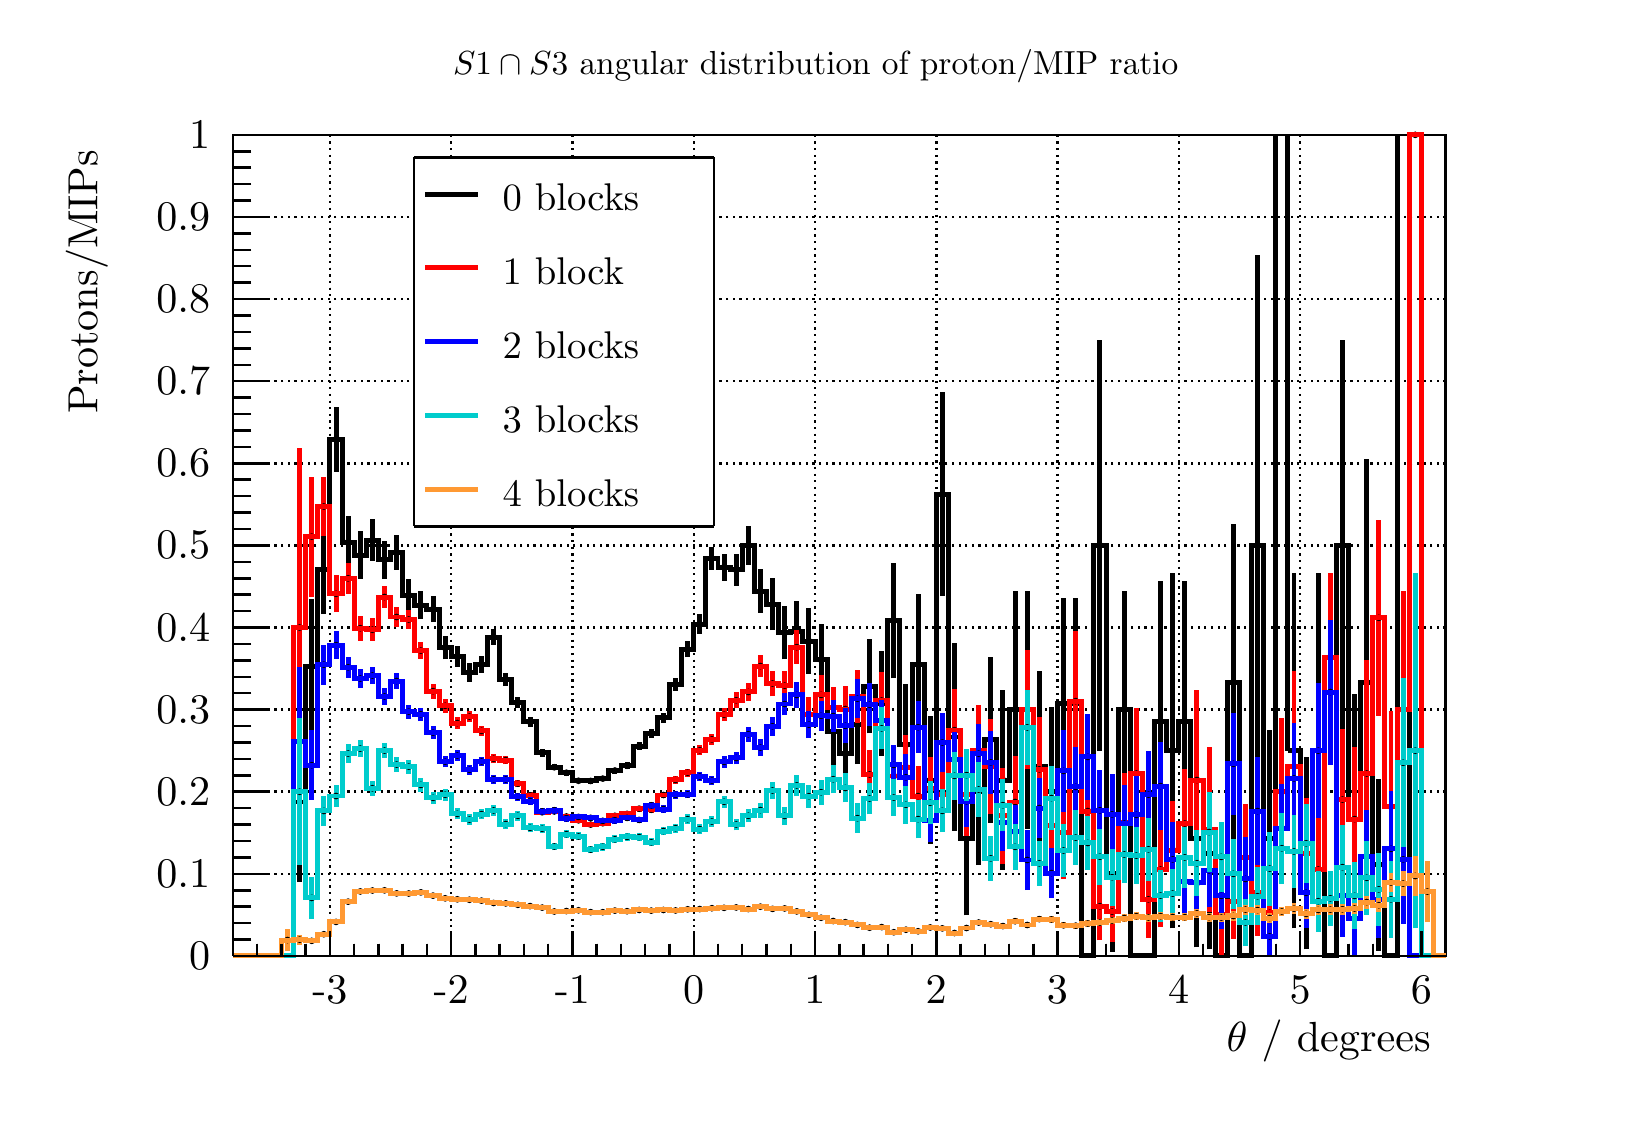
\begin{tikzpicture}
\pgfdeclareplotmark{cross} {
\pgfpathmoveto{\pgfpoint{-0.3\pgfplotmarksize}{\pgfplotmarksize}}
\pgfpathlineto{\pgfpoint{+0.3\pgfplotmarksize}{\pgfplotmarksize}}
\pgfpathlineto{\pgfpoint{+0.3\pgfplotmarksize}{0.3\pgfplotmarksize}}
\pgfpathlineto{\pgfpoint{+1\pgfplotmarksize}{0.3\pgfplotmarksize}}
\pgfpathlineto{\pgfpoint{+1\pgfplotmarksize}{-0.3\pgfplotmarksize}}
\pgfpathlineto{\pgfpoint{+0.3\pgfplotmarksize}{-0.3\pgfplotmarksize}}
\pgfpathlineto{\pgfpoint{+0.3\pgfplotmarksize}{-1.\pgfplotmarksize}}
\pgfpathlineto{\pgfpoint{-0.3\pgfplotmarksize}{-1.\pgfplotmarksize}}
\pgfpathlineto{\pgfpoint{-0.3\pgfplotmarksize}{-0.3\pgfplotmarksize}}
\pgfpathlineto{\pgfpoint{-1.\pgfplotmarksize}{-0.3\pgfplotmarksize}}
\pgfpathlineto{\pgfpoint{-1.\pgfplotmarksize}{0.3\pgfplotmarksize}}
\pgfpathlineto{\pgfpoint{-0.3\pgfplotmarksize}{0.3\pgfplotmarksize}}
\pgfpathclose
\pgfusepathqstroke
}
\pgfdeclareplotmark{cross*} {
\pgfpathmoveto{\pgfpoint{-0.3\pgfplotmarksize}{\pgfplotmarksize}}
\pgfpathlineto{\pgfpoint{+0.3\pgfplotmarksize}{\pgfplotmarksize}}
\pgfpathlineto{\pgfpoint{+0.3\pgfplotmarksize}{0.3\pgfplotmarksize}}
\pgfpathlineto{\pgfpoint{+1\pgfplotmarksize}{0.3\pgfplotmarksize}}
\pgfpathlineto{\pgfpoint{+1\pgfplotmarksize}{-0.3\pgfplotmarksize}}
\pgfpathlineto{\pgfpoint{+0.3\pgfplotmarksize}{-0.3\pgfplotmarksize}}
\pgfpathlineto{\pgfpoint{+0.3\pgfplotmarksize}{-1.\pgfplotmarksize}}
\pgfpathlineto{\pgfpoint{-0.3\pgfplotmarksize}{-1.\pgfplotmarksize}}
\pgfpathlineto{\pgfpoint{-0.3\pgfplotmarksize}{-0.3\pgfplotmarksize}}
\pgfpathlineto{\pgfpoint{-1.\pgfplotmarksize}{-0.3\pgfplotmarksize}}
\pgfpathlineto{\pgfpoint{-1.\pgfplotmarksize}{0.3\pgfplotmarksize}}
\pgfpathlineto{\pgfpoint{-0.3\pgfplotmarksize}{0.3\pgfplotmarksize}}
\pgfpathclose
\pgfusepathqfillstroke
}
\pgfdeclareplotmark{newstar} {
\pgfpathmoveto{\pgfqpoint{0pt}{\pgfplotmarksize}}
\pgfpathlineto{\pgfqpointpolar{44}{0.5\pgfplotmarksize}}
\pgfpathlineto{\pgfqpointpolar{18}{\pgfplotmarksize}}
\pgfpathlineto{\pgfqpointpolar{-20}{0.5\pgfplotmarksize}}
\pgfpathlineto{\pgfqpointpolar{-54}{\pgfplotmarksize}}
\pgfpathlineto{\pgfqpointpolar{-90}{0.5\pgfplotmarksize}}
\pgfpathlineto{\pgfqpointpolar{234}{\pgfplotmarksize}}
\pgfpathlineto{\pgfqpointpolar{198}{0.5\pgfplotmarksize}}
\pgfpathlineto{\pgfqpointpolar{162}{\pgfplotmarksize}}
\pgfpathlineto{\pgfqpointpolar{134}{0.5\pgfplotmarksize}}
\pgfpathclose
\pgfusepathqstroke
}
\pgfdeclareplotmark{newstar*} {
\pgfpathmoveto{\pgfqpoint{0pt}{\pgfplotmarksize}}
\pgfpathlineto{\pgfqpointpolar{44}{0.5\pgfplotmarksize}}
\pgfpathlineto{\pgfqpointpolar{18}{\pgfplotmarksize}}
\pgfpathlineto{\pgfqpointpolar{-20}{0.5\pgfplotmarksize}}
\pgfpathlineto{\pgfqpointpolar{-54}{\pgfplotmarksize}}
\pgfpathlineto{\pgfqpointpolar{-90}{0.5\pgfplotmarksize}}
\pgfpathlineto{\pgfqpointpolar{234}{\pgfplotmarksize}}
\pgfpathlineto{\pgfqpointpolar{198}{0.5\pgfplotmarksize}}
\pgfpathlineto{\pgfqpointpolar{162}{\pgfplotmarksize}}
\pgfpathlineto{\pgfqpointpolar{134}{0.5\pgfplotmarksize}}
\pgfpathclose
\pgfusepathqfillstroke
}
\definecolor{c}{rgb}{1,1,1};
\draw [color=c, fill=c] (0,0) rectangle (20,13.5429);
\draw [color=c, fill=c] (2.6,1.76057) rectangle (18,12.1886);
\definecolor{c}{rgb}{0,0,0};
\draw [c,line width=0.9] (2.6,1.76057) -- (2.6,12.1886) -- (18,12.1886) -- (18,1.76057) -- (2.6,1.76057);
\definecolor{c}{rgb}{1,1,1};
\draw [color=c, fill=c] (2.6,1.76057) rectangle (18,12.1886);
\definecolor{c}{rgb}{0,0,0};
\draw [c,line width=0.9] (2.6,1.76057) -- (2.6,12.1886) -- (18,12.1886) -- (18,1.76057) -- (2.6,1.76057);
\draw [c,line width=0.9] (2.6,1.76057) -- (18,1.76057);
\draw [c,dash pattern=on 0.80pt off 1.60pt ,line width=0.9] (3.832,12.1886) -- (3.832,1.76057);
\draw [c,dash pattern=on 0.80pt off 1.60pt ,line width=0.9] (5.372,12.1886) -- (5.372,1.76057);
\draw [c,dash pattern=on 0.80pt off 1.60pt ,line width=0.9] (6.912,12.1886) -- (6.912,1.76057);
\draw [c,dash pattern=on 0.80pt off 1.60pt ,line width=0.9] (8.452,12.1886) -- (8.452,1.76057);
\draw [c,dash pattern=on 0.80pt off 1.60pt ,line width=0.9] (9.992,12.1886) -- (9.992,1.76057);
\draw [c,dash pattern=on 0.80pt off 1.60pt ,line width=0.9] (11.532,12.1886) -- (11.532,1.76057);
\draw [c,dash pattern=on 0.80pt off 1.60pt ,line width=0.9] (13.072,12.1886) -- (13.072,1.76057);
\draw [c,dash pattern=on 0.80pt off 1.60pt ,line width=0.9] (14.612,12.1886) -- (14.612,1.76057);
\draw [c,dash pattern=on 0.80pt off 1.60pt ,line width=0.9] (16.152,12.1886) -- (16.152,1.76057);
\draw [c,dash pattern=on 0.80pt off 1.60pt ,line width=0.9] (17.692,12.1886) -- (17.692,1.76057);
\draw [c,dash pattern=on 0.80pt off 1.60pt ,line width=0.9] (3.832,12.1886) -- (3.832,1.76057);
\draw [c,dash pattern=on 0.80pt off 1.60pt ,line width=0.9] (17.692,12.1886) -- (17.692,1.76057);
\draw [c,line width=0.9] (2.6,1.76057) -- (2.6,12.1886);
\draw [c,dash pattern=on 0.80pt off 1.60pt ,line width=0.9] (18,1.76057) -- (2.6,1.76057);
\draw [c,dash pattern=on 0.80pt off 1.60pt ,line width=0.9] (18,2.80337) -- (2.6,2.80337);
\draw [c,dash pattern=on 0.80pt off 1.60pt ,line width=0.9] (18,3.84617) -- (2.6,3.84617);
\draw [c,dash pattern=on 0.80pt off 1.60pt ,line width=0.9] (18,4.88897) -- (2.6,4.88897);
\draw [c,dash pattern=on 0.80pt off 1.60pt ,line width=0.9] (18,5.93177) -- (2.6,5.93177);
\draw [c,dash pattern=on 0.80pt off 1.60pt ,line width=0.9] (18,6.97457) -- (2.6,6.97457);
\draw [c,dash pattern=on 0.80pt off 1.60pt ,line width=0.9] (18,8.01737) -- (2.6,8.01737);
\draw [c,dash pattern=on 0.80pt off 1.60pt ,line width=0.9] (18,9.06017) -- (2.6,9.06017);
\draw [c,dash pattern=on 0.80pt off 1.60pt ,line width=0.9] (18,10.103) -- (2.6,10.103);
\draw [c,dash pattern=on 0.80pt off 1.60pt ,line width=0.9] (18,11.1458) -- (2.6,11.1458);
\draw [c,dash pattern=on 0.80pt off 1.60pt ,line width=0.9] (18,12.1886) -- (2.6,12.1886);
\definecolor{c}{rgb}{0,0,0.6};
\draw [c,line width=0.9] (2.6,1.76057) -- (2.754,1.76057) -- (2.754,1.76057) -- (2.908,1.76057) -- (2.908,1.76057) -- (3.062,1.76057) -- (3.062,1.76057) -- (3.216,1.76057) -- (3.216,1.76057) -- (3.37,1.76057) -- (3.37,1.76057) -- (3.524,1.76057) --
 (3.524,1.76057) -- (3.678,1.76057) -- (3.678,1.76057) -- (3.832,1.76057) -- (3.832,1.76057) -- (3.986,1.76057) -- (3.986,1.76057) -- (4.14,1.76057) -- (4.14,1.76057) -- (4.294,1.76057) -- (4.294,1.76057) -- (4.448,1.76057) -- (4.448,1.76057) --
 (4.602,1.76057) -- (4.602,1.76057) -- (4.756,1.76057) -- (4.756,1.76057) -- (4.91,1.76057) -- (4.91,1.76057) -- (5.064,1.76057) -- (5.064,1.76057) -- (5.218,1.76057) -- (5.218,1.76057) -- (5.372,1.76057) -- (5.372,1.76057) -- (5.526,1.76057) --
 (5.526,1.76057) -- (5.68,1.76057) -- (5.68,1.76057) -- (5.834,1.76057) -- (5.834,1.76057) -- (5.988,1.76057) -- (5.988,1.76057) -- (6.142,1.76057) -- (6.142,1.76057) -- (6.296,1.76057) -- (6.296,1.76057) -- (6.45,1.76057) -- (6.45,1.76057) --
 (6.604,1.76057) -- (6.604,1.76057) -- (6.758,1.76057) -- (6.758,1.76057) -- (6.912,1.76057) -- (6.912,1.76057) -- (7.066,1.76057) -- (7.066,1.76057) -- (7.22,1.76057) -- (7.22,1.76057) -- (7.374,1.76057) -- (7.374,1.76057) -- (7.528,1.76057) --
 (7.528,1.76057) -- (7.682,1.76057) -- (7.682,1.76057) -- (7.836,1.76057) -- (7.836,1.76057) -- (7.99,1.76057) -- (7.99,1.76057) -- (8.144,1.76057) -- (8.144,1.76057) -- (8.298,1.76057) -- (8.298,1.76057) -- (8.452,1.76057) -- (8.452,1.76057) --
 (8.606,1.76057) -- (8.606,1.76057) -- (8.76,1.76057) -- (8.76,1.76057) -- (8.914,1.76057) -- (8.914,1.76057) -- (9.068,1.76057) -- (9.068,1.76057) -- (9.222,1.76057) -- (9.222,1.76057) -- (9.376,1.76057) -- (9.376,1.76057) -- (9.53,1.76057) --
 (9.53,1.76057) -- (9.684,1.76057) -- (9.684,1.76057) -- (9.838,1.76057) -- (9.838,1.76057) -- (9.992,1.76057) -- (9.992,1.76057) -- (10.146,1.76057) -- (10.146,1.76057) -- (10.3,1.76057) -- (10.3,1.76057) -- (10.454,1.76057) -- (10.454,1.76057) --
 (10.608,1.76057) -- (10.608,1.76057) -- (10.762,1.76057) -- (10.762,1.76057) -- (10.916,1.76057) -- (10.916,1.76057) -- (11.07,1.76057) -- (11.07,1.76057) -- (11.224,1.76057) -- (11.224,1.76057) -- (11.378,1.76057) -- (11.378,1.76057) --
 (11.532,1.76057) -- (11.532,1.76057) -- (11.686,1.76057) -- (11.686,1.76057) -- (11.84,1.76057) -- (11.84,1.76057) -- (11.994,1.76057) -- (11.994,1.76057) -- (12.148,1.76057) -- (12.148,1.76057) -- (12.302,1.76057) -- (12.302,1.76057) --
 (12.456,1.76057) -- (12.456,1.76057) -- (12.61,1.76057) -- (12.61,1.76057) -- (12.764,1.76057) -- (12.764,1.76057) -- (12.918,1.76057) -- (12.918,1.76057) -- (13.072,1.76057) -- (13.072,1.76057) -- (13.226,1.76057) -- (13.226,1.76057) --
 (13.38,1.76057) -- (13.38,1.76057) -- (13.534,1.76057) -- (13.534,1.76057) -- (13.688,1.76057) -- (13.688,1.76057) -- (13.842,1.76057) -- (13.842,1.76057) -- (13.996,1.76057) -- (13.996,1.76057) -- (14.15,1.76057) -- (14.15,1.76057) --
 (14.304,1.76057) -- (14.304,1.76057) -- (14.458,1.76057) -- (14.458,1.76057) -- (14.612,1.76057) -- (14.612,1.76057) -- (14.766,1.76057) -- (14.766,1.76057) -- (14.92,1.76057) -- (14.92,1.76057) -- (15.074,1.76057) -- (15.074,1.76057) --
 (15.228,1.76057) -- (15.228,1.76057) -- (15.382,1.76057) -- (15.382,1.76057) -- (15.536,1.76057) -- (15.536,1.76057) -- (15.69,1.76057) -- (15.69,1.76057) -- (15.844,1.76057) -- (15.844,1.76057) -- (15.998,1.76057) -- (15.998,1.76057) --
 (16.152,1.76057) -- (16.152,1.76057) -- (16.306,1.76057) -- (16.306,1.76057) -- (16.46,1.76057) -- (16.46,1.76057) -- (16.614,1.76057) -- (16.614,1.76057) -- (16.768,1.76057) -- (16.768,1.76057) -- (16.922,1.76057) -- (16.922,1.76057) --
 (17.076,1.76057) -- (17.076,1.76057) -- (17.23,1.76057) -- (17.23,1.76057) -- (17.384,1.76057) -- (17.384,1.76057) -- (17.538,1.76057) -- (17.538,1.76057) -- (17.692,1.76057) -- (17.692,1.76057) -- (17.846,1.76057) -- (17.846,1.76057) --
 (18,1.76057);
\definecolor{c}{rgb}{0,0,0};
\draw [c,line width=0.9] (2.6,1.76057) -- (18,1.76057);
\draw [c,line width=0.9] (3.832,2.07341) -- (3.832,1.76057);
\draw [c,line width=0.9] (4.14,1.91699) -- (4.14,1.76057);
\draw [c,line width=0.9] (4.448,1.91699) -- (4.448,1.76057);
\draw [c,line width=0.9] (4.756,1.91699) -- (4.756,1.76057);
\draw [c,line width=0.9] (5.064,1.91699) -- (5.064,1.76057);
\draw [c,line width=0.9] (5.372,2.07341) -- (5.372,1.76057);
\draw [c,line width=0.9] (5.68,1.91699) -- (5.68,1.76057);
\draw [c,line width=0.9] (5.988,1.91699) -- (5.988,1.76057);
\draw [c,line width=0.9] (6.296,1.91699) -- (6.296,1.76057);
\draw [c,line width=0.9] (6.604,1.91699) -- (6.604,1.76057);
\draw [c,line width=0.9] (6.912,2.07341) -- (6.912,1.76057);
\draw [c,line width=0.9] (7.22,1.91699) -- (7.22,1.76057);
\draw [c,line width=0.9] (7.528,1.91699) -- (7.528,1.76057);
\draw [c,line width=0.9] (7.836,1.91699) -- (7.836,1.76057);
\draw [c,line width=0.9] (8.144,1.91699) -- (8.144,1.76057);
\draw [c,line width=0.9] (8.452,2.07341) -- (8.452,1.76057);
\draw [c,line width=0.9] (8.76,1.91699) -- (8.76,1.76057);
\draw [c,line width=0.9] (9.068,1.91699) -- (9.068,1.76057);
\draw [c,line width=0.9] (9.376,1.91699) -- (9.376,1.76057);
\draw [c,line width=0.9] (9.684,1.91699) -- (9.684,1.76057);
\draw [c,line width=0.9] (9.992,2.07341) -- (9.992,1.76057);
\draw [c,line width=0.9] (10.3,1.91699) -- (10.3,1.76057);
\draw [c,line width=0.9] (10.608,1.91699) -- (10.608,1.76057);
\draw [c,line width=0.9] (10.916,1.91699) -- (10.916,1.76057);
\draw [c,line width=0.9] (11.224,1.91699) -- (11.224,1.76057);
\draw [c,line width=0.9] (11.532,2.07341) -- (11.532,1.76057);
\draw [c,line width=0.9] (11.84,1.91699) -- (11.84,1.76057);
\draw [c,line width=0.9] (12.148,1.91699) -- (12.148,1.76057);
\draw [c,line width=0.9] (12.456,1.91699) -- (12.456,1.76057);
\draw [c,line width=0.9] (12.764,1.91699) -- (12.764,1.76057);
\draw [c,line width=0.9] (13.072,2.07341) -- (13.072,1.76057);
\draw [c,line width=0.9] (13.38,1.91699) -- (13.38,1.76057);
\draw [c,line width=0.9] (13.688,1.91699) -- (13.688,1.76057);
\draw [c,line width=0.9] (13.996,1.91699) -- (13.996,1.76057);
\draw [c,line width=0.9] (14.304,1.91699) -- (14.304,1.76057);
\draw [c,line width=0.9] (14.612,2.07341) -- (14.612,1.76057);
\draw [c,line width=0.9] (14.92,1.91699) -- (14.92,1.76057);
\draw [c,line width=0.9] (15.228,1.91699) -- (15.228,1.76057);
\draw [c,line width=0.9] (15.536,1.91699) -- (15.536,1.76057);
\draw [c,line width=0.9] (15.844,1.91699) -- (15.844,1.76057);
\draw [c,line width=0.9] (16.152,2.07341) -- (16.152,1.76057);
\draw [c,line width=0.9] (16.46,1.91699) -- (16.46,1.76057);
\draw [c,line width=0.9] (16.768,1.91699) -- (16.768,1.76057);
\draw [c,line width=0.9] (17.076,1.91699) -- (17.076,1.76057);
\draw [c,line width=0.9] (17.384,1.91699) -- (17.384,1.76057);
\draw [c,line width=0.9] (17.692,2.07341) -- (17.692,1.76057);
\draw [c,line width=0.9] (3.832,2.07341) -- (3.832,1.76057);
\draw [c,line width=0.9] (3.524,1.91699) -- (3.524,1.76057);
\draw [c,line width=0.9] (3.216,1.91699) -- (3.216,1.76057);
\draw [c,line width=0.9] (2.908,1.91699) -- (2.908,1.76057);
\draw [c,line width=0.9] (17.692,2.07341) -- (17.692,1.76057);
\draw [anchor=base] (3.832,1.15114) node[scale=1.52295, color=c, rotate=0]{-3};
\draw [anchor=base] (5.372,1.15114) node[scale=1.52295, color=c, rotate=0]{-2};
\draw [anchor=base] (6.912,1.15114) node[scale=1.52295, color=c, rotate=0]{-1};
\draw [anchor=base] (8.452,1.15114) node[scale=1.52295, color=c, rotate=0]{0};
\draw [anchor=base] (9.992,1.15114) node[scale=1.52295, color=c, rotate=0]{1};
\draw [anchor=base] (11.532,1.15114) node[scale=1.52295, color=c, rotate=0]{2};
\draw [anchor=base] (13.072,1.15114) node[scale=1.52295, color=c, rotate=0]{3};
\draw [anchor=base] (14.612,1.15114) node[scale=1.52295, color=c, rotate=0]{4};
\draw [anchor=base] (16.152,1.15114) node[scale=1.52295, color=c, rotate=0]{5};
\draw [anchor=base] (17.692,1.15114) node[scale=1.52295, color=c, rotate=0]{6};
\draw [anchor= east] (18,0.677143) node[scale=1.52295, color=c, rotate=0]{$ \theta$ / degrees};
\draw [c,line width=0.9] (2.6,1.76057) -- (2.6,12.1886);
\draw [c,line width=0.9] (3.062,1.76057) -- (2.6,1.76057);
\draw [c,line width=0.9] (2.831,1.96913) -- (2.6,1.96913);
\draw [c,line width=0.9] (2.831,2.17769) -- (2.6,2.17769);
\draw [c,line width=0.9] (2.831,2.38625) -- (2.6,2.38625);
\draw [c,line width=0.9] (2.831,2.59481) -- (2.6,2.59481);
\draw [c,line width=0.9] (3.062,2.80337) -- (2.6,2.80337);
\draw [c,line width=0.9] (2.831,3.01193) -- (2.6,3.01193);
\draw [c,line width=0.9] (2.831,3.22049) -- (2.6,3.22049);
\draw [c,line width=0.9] (2.831,3.42905) -- (2.6,3.42905);
\draw [c,line width=0.9] (2.831,3.63761) -- (2.6,3.63761);
\draw [c,line width=0.9] (3.062,3.84617) -- (2.6,3.84617);
\draw [c,line width=0.9] (2.831,4.05473) -- (2.6,4.05473);
\draw [c,line width=0.9] (2.831,4.26329) -- (2.6,4.26329);
\draw [c,line width=0.9] (2.831,4.47185) -- (2.6,4.47185);
\draw [c,line width=0.9] (2.831,4.68041) -- (2.6,4.68041);
\draw [c,line width=0.9] (3.062,4.88897) -- (2.6,4.88897);
\draw [c,line width=0.9] (2.831,5.09753) -- (2.6,5.09753);
\draw [c,line width=0.9] (2.831,5.30609) -- (2.6,5.30609);
\draw [c,line width=0.9] (2.831,5.51465) -- (2.6,5.51465);
\draw [c,line width=0.9] (2.831,5.72321) -- (2.6,5.72321);
\draw [c,line width=0.9] (3.062,5.93177) -- (2.6,5.93177);
\draw [c,line width=0.9] (2.831,6.14033) -- (2.6,6.14033);
\draw [c,line width=0.9] (2.831,6.34889) -- (2.6,6.34889);
\draw [c,line width=0.9] (2.831,6.55745) -- (2.6,6.55745);
\draw [c,line width=0.9] (2.831,6.76601) -- (2.6,6.76601);
\draw [c,line width=0.9] (3.062,6.97457) -- (2.6,6.97457);
\draw [c,line width=0.9] (2.831,7.18313) -- (2.6,7.18313);
\draw [c,line width=0.9] (2.831,7.39169) -- (2.6,7.39169);
\draw [c,line width=0.9] (2.831,7.60025) -- (2.6,7.60025);
\draw [c,line width=0.9] (2.831,7.80881) -- (2.6,7.80881);
\draw [c,line width=0.9] (3.062,8.01737) -- (2.6,8.01737);
\draw [c,line width=0.9] (2.831,8.22593) -- (2.6,8.22593);
\draw [c,line width=0.9] (2.831,8.43449) -- (2.6,8.43449);
\draw [c,line width=0.9] (2.831,8.64305) -- (2.6,8.64305);
\draw [c,line width=0.9] (2.831,8.85161) -- (2.6,8.85161);
\draw [c,line width=0.9] (3.062,9.06017) -- (2.6,9.06017);
\draw [c,line width=0.9] (2.831,9.26873) -- (2.6,9.26873);
\draw [c,line width=0.9] (2.831,9.47729) -- (2.6,9.47729);
\draw [c,line width=0.9] (2.831,9.68585) -- (2.6,9.68585);
\draw [c,line width=0.9] (2.831,9.89441) -- (2.6,9.89441);
\draw [c,line width=0.9] (3.062,10.103) -- (2.6,10.103);
\draw [c,line width=0.9] (2.831,10.3115) -- (2.6,10.3115);
\draw [c,line width=0.9] (2.831,10.5201) -- (2.6,10.5201);
\draw [c,line width=0.9] (2.831,10.7287) -- (2.6,10.7287);
\draw [c,line width=0.9] (2.831,10.9372) -- (2.6,10.9372);
\draw [c,line width=0.9] (3.062,11.1458) -- (2.6,11.1458);
\draw [c,line width=0.9] (2.831,11.3543) -- (2.6,11.3543);
\draw [c,line width=0.9] (2.831,11.5629) -- (2.6,11.5629);
\draw [c,line width=0.9] (2.831,11.7715) -- (2.6,11.7715);
\draw [c,line width=0.9] (2.831,11.98) -- (2.6,11.98);
\draw [c,line width=0.9] (3.062,12.1886) -- (2.6,12.1886);
\draw [anchor= east] (2.5,1.76057) node[scale=1.52295, color=c, rotate=0]{0};
\draw [anchor= east] (2.5,2.80337) node[scale=1.52295, color=c, rotate=0]{0.1};
\draw [anchor= east] (2.5,3.84617) node[scale=1.52295, color=c, rotate=0]{0.2};
\draw [anchor= east] (2.5,4.88897) node[scale=1.52295, color=c, rotate=0]{0.3};
\draw [anchor= east] (2.5,5.93177) node[scale=1.52295, color=c, rotate=0]{0.4};
\draw [anchor= east] (2.5,6.97457) node[scale=1.52295, color=c, rotate=0]{0.5};
\draw [anchor= east] (2.5,8.01737) node[scale=1.52295, color=c, rotate=0]{0.6};
\draw [anchor= east] (2.5,9.06017) node[scale=1.52295, color=c, rotate=0]{0.7};
\draw [anchor= east] (2.5,10.103) node[scale=1.52295, color=c, rotate=0]{0.8};
\draw [anchor= east] (2.5,11.1458) node[scale=1.52295, color=c, rotate=0]{0.9};
\draw [anchor= east] (2.5,12.1886) node[scale=1.52295, color=c, rotate=0]{1};
\draw [anchor= east] (0.742857,12.1886) node[scale=1.52295, color=c, rotate=90]{  Protons/MIPs};
\draw [c,line width=1.8] (3.447,2.69828) -- (3.447,3.71582);
\draw [c,line width=1.8] (3.447,3.71582) -- (3.447,4.73337);
\foreach \P in {(3.447,3.71582)}{\draw[mark options={color=c,fill=c},mark size=2.402402pt,mark=*,mark size=1pt] plot coordinates {\P};}
\draw [c,line width=1.8] (3.601,4.5864) -- (3.601,5.44104);
\draw [c,line width=1.8] (3.601,5.44104) -- (3.601,6.29568);
\foreach \P in {(3.601,5.44104)}{\draw[mark options={color=c,fill=c},mark size=2.402402pt,mark=*,mark size=1pt] plot coordinates {\P};}
\draw [c,line width=1.8] (3.755,6.10331) -- (3.755,6.66787);
\draw [c,line width=1.8] (3.755,6.66787) -- (3.755,7.23242);
\foreach \P in {(3.755,6.66787)}{\draw[mark options={color=c,fill=c},mark size=2.402402pt,mark=*,mark size=1pt] plot coordinates {\P};}
\draw [c,line width=1.8] (3.909,7.91132) -- (3.909,8.32123);
\draw [c,line width=1.8] (3.909,8.32123) -- (3.909,8.73115);
\foreach \P in {(3.909,8.32123)}{\draw[mark options={color=c,fill=c},mark size=2.402402pt,mark=*,mark size=1pt] plot coordinates {\P};}
\draw [c,line width=1.8] (4.063,6.68653) -- (4.063,7.01628);
\draw [c,line width=1.8] (4.063,7.01628) -- (4.063,7.34604);
\foreach \P in {(4.063,7.01628)}{\draw[mark options={color=c,fill=c},mark size=2.402402pt,mark=*,mark size=1pt] plot coordinates {\P};}
\draw [c,line width=1.8] (4.217,6.54736) -- (4.217,6.85085);
\draw [c,line width=1.8] (4.217,6.85085) -- (4.217,7.15433);
\foreach \P in {(4.217,6.85085)}{\draw[mark options={color=c,fill=c},mark size=2.402402pt,mark=*,mark size=1pt] plot coordinates {\P};}
\draw [c,line width=1.8] (4.371,6.77692) -- (4.371,7.04194);
\draw [c,line width=1.8] (4.371,7.04194) -- (4.371,7.30696);
\foreach \P in {(4.371,7.04194)}{\draw[mark options={color=c,fill=c},mark size=2.402402pt,mark=*,mark size=1pt] plot coordinates {\P};}
\draw [c,line width=1.8] (4.525,6.54627) -- (4.525,6.79082);
\draw [c,line width=1.8] (4.525,6.79082) -- (4.525,7.03537);
\foreach \P in {(4.525,6.79082)}{\draw[mark options={color=c,fill=c},mark size=2.402402pt,mark=*,mark size=1pt] plot coordinates {\P};}
\draw [c,line width=1.8] (4.679,6.66261) -- (4.679,6.88212);
\draw [c,line width=1.8] (4.679,6.88212) -- (4.679,7.10164);
\foreach \P in {(4.679,6.88212)}{\draw[mark options={color=c,fill=c},mark size=2.402402pt,mark=*,mark size=1pt] plot coordinates {\P};}
\draw [c,line width=1.8] (4.833,6.14124) -- (4.833,6.34378);
\draw [c,line width=1.8] (4.833,6.34378) -- (4.833,6.54632);
\foreach \P in {(4.833,6.34378)}{\draw[mark options={color=c,fill=c},mark size=2.402402pt,mark=*,mark size=1pt] plot coordinates {\P};}
\draw [c,line width=1.8] (4.987,6.03439) -- (4.987,6.21354);
\draw [c,line width=1.8] (4.987,6.21354) -- (4.987,6.39269);
\foreach \P in {(4.987,6.21354)}{\draw[mark options={color=c,fill=c},mark size=2.402402pt,mark=*,mark size=1pt] plot coordinates {\P};}
\draw [c,line width=1.8] (5.141,6.00133) -- (5.141,6.16587);
\draw [c,line width=1.8] (5.141,6.16587) -- (5.141,6.33041);
\foreach \P in {(5.141,6.16587)}{\draw[mark options={color=c,fill=c},mark size=2.402402pt,mark=*,mark size=1pt] plot coordinates {\P};}
\draw [c,line width=1.8] (5.295,5.52618) -- (5.295,5.67328);
\draw [c,line width=1.8] (5.295,5.67328) -- (5.295,5.82039);
\foreach \P in {(5.295,5.67328)}{\draw[mark options={color=c,fill=c},mark size=2.402402pt,mark=*,mark size=1pt] plot coordinates {\P};}
\draw [c,line width=1.8] (5.449,5.43471) -- (5.449,5.5688);
\draw [c,line width=1.8] (5.449,5.5688) -- (5.449,5.70289);
\foreach \P in {(5.449,5.5688)}{\draw[mark options={color=c,fill=c},mark size=2.402402pt,mark=*,mark size=1pt] plot coordinates {\P};}
\draw [c,line width=1.8] (5.603,5.24489) -- (5.603,5.36319);
\draw [c,line width=1.8] (5.603,5.36319) -- (5.603,5.48149);
\foreach \P in {(5.603,5.36319)}{\draw[mark options={color=c,fill=c},mark size=2.402402pt,mark=*,mark size=1pt] plot coordinates {\P};}
\draw [c,line width=1.8] (5.757,5.35586) -- (5.757,5.46365);
\draw [c,line width=1.8] (5.757,5.46365) -- (5.757,5.57145);
\foreach \P in {(5.757,5.46365)}{\draw[mark options={color=c,fill=c},mark size=2.402402pt,mark=*,mark size=1pt] plot coordinates {\P};}
\draw [c,line width=1.8] (5.911,5.71068) -- (5.911,5.80974);
\draw [c,line width=1.8] (5.911,5.80974) -- (5.911,5.9088);
\foreach \P in {(5.911,5.80974)}{\draw[mark options={color=c,fill=c},mark size=2.402402pt,mark=*,mark size=1pt] plot coordinates {\P};}
\draw [c,line width=1.8] (6.065,5.18882) -- (6.065,5.27358);
\draw [c,line width=1.8] (6.065,5.27358) -- (6.065,5.35835);
\foreach \P in {(6.065,5.27358)}{\draw[mark options={color=c,fill=c},mark size=2.402402pt,mark=*,mark size=1pt] plot coordinates {\P};}
\draw [c,line width=1.8] (6.219,4.90855) -- (6.219,4.97895);
\draw [c,line width=1.8] (6.219,4.97895) -- (6.219,5.04935);
\foreach \P in {(6.219,4.97895)}{\draw[mark options={color=c,fill=c},mark size=2.402402pt,mark=*,mark size=1pt] plot coordinates {\P};}
\draw [c,line width=1.8] (6.373,4.67359) -- (6.373,4.73253);
\draw [c,line width=1.8] (6.373,4.73253) -- (6.373,4.79147);
\foreach \P in {(6.373,4.73253)}{\draw[mark options={color=c,fill=c},mark size=2.402402pt,mark=*,mark size=1pt] plot coordinates {\P};}
\draw [c,line width=1.8] (6.527,4.29323) -- (6.527,4.34135);
\draw [c,line width=1.8] (6.527,4.34135) -- (6.527,4.38946);
\foreach \P in {(6.527,4.34135)}{\draw[mark options={color=c,fill=c},mark size=2.402402pt,mark=*,mark size=1pt] plot coordinates {\P};}
\draw [c,line width=1.8] (6.681,4.11642) -- (6.681,4.1571);
\draw [c,line width=1.8] (6.681,4.1571) -- (6.681,4.19778);
\foreach \P in {(6.681,4.1571)}{\draw[mark options={color=c,fill=c},mark size=2.402402pt,mark=*,mark size=1pt] plot coordinates {\P};}
\draw [c,line width=1.8] (6.835,4.05142) -- (6.835,4.08804);
\draw [c,line width=1.8] (6.835,4.08804) -- (6.835,4.12465);
\foreach \P in {(6.835,4.08804)}{\draw[mark options={color=c,fill=c},mark size=2.402402pt,mark=*,mark size=1pt] plot coordinates {\P};}
\draw [c,line width=1.8] (6.989,3.95156) -- (6.989,3.98547);
\draw [c,line width=1.8] (6.989,3.98547) -- (6.989,4.01939);
\foreach \P in {(6.989,3.98547)}{\draw[mark options={color=c,fill=c},mark size=2.402402pt,mark=*,mark size=1pt] plot coordinates {\P};}
\draw [c,line width=1.8] (7.143,3.94992) -- (7.143,3.98352);
\draw [c,line width=1.8] (7.143,3.98352) -- (7.143,4.01712);
\foreach \P in {(7.143,3.98352)}{\draw[mark options={color=c,fill=c},mark size=2.402402pt,mark=*,mark size=1pt] plot coordinates {\P};}
\draw [c,line width=1.8] (7.297,3.97822) -- (7.297,4.013);
\draw [c,line width=1.8] (7.297,4.013) -- (7.297,4.04777);
\foreach \P in {(7.297,4.013)}{\draw[mark options={color=c,fill=c},mark size=2.402402pt,mark=*,mark size=1pt] plot coordinates {\P};}
\draw [c,line width=1.8] (7.451,4.07786) -- (7.451,4.11597);
\draw [c,line width=1.8] (7.451,4.11597) -- (7.451,4.15409);
\foreach \P in {(7.451,4.11597)}{\draw[mark options={color=c,fill=c},mark size=2.402402pt,mark=*,mark size=1pt] plot coordinates {\P};}
\draw [c,line width=1.8] (7.605,4.13387) -- (7.605,4.17615);
\draw [c,line width=1.8] (7.605,4.17615) -- (7.605,4.21843);
\foreach \P in {(7.605,4.17615)}{\draw[mark options={color=c,fill=c},mark size=2.402402pt,mark=*,mark size=1pt] plot coordinates {\P};}
\draw [c,line width=1.8] (7.759,4.37721) -- (7.759,4.42618);
\draw [c,line width=1.8] (7.759,4.42618) -- (7.759,4.47514);
\foreach \P in {(7.759,4.42618)}{\draw[mark options={color=c,fill=c},mark size=2.402402pt,mark=*,mark size=1pt] plot coordinates {\P};}
\draw [c,line width=1.8] (7.913,4.52827) -- (7.913,4.58456);
\draw [c,line width=1.8] (7.913,4.58456) -- (7.913,4.64086);
\foreach \P in {(7.913,4.58456)}{\draw[mark options={color=c,fill=c},mark size=2.402402pt,mark=*,mark size=1pt] plot coordinates {\P};}
\draw [c,line width=1.8] (8.067,4.71813) -- (8.067,4.78436);
\draw [c,line width=1.8] (8.067,4.78436) -- (8.067,4.8506);
\foreach \P in {(8.067,4.78436)}{\draw[mark options={color=c,fill=c},mark size=2.402402pt,mark=*,mark size=1pt] plot coordinates {\P};}
\draw [c,line width=1.8] (8.221,5.13176) -- (8.221,5.21346);
\draw [c,line width=1.8] (8.221,5.21346) -- (8.221,5.29515);
\foreach \P in {(8.221,5.21346)}{\draw[mark options={color=c,fill=c},mark size=2.402402pt,mark=*,mark size=1pt] plot coordinates {\P};}
\draw [c,line width=1.8] (8.375,5.55691) -- (8.375,5.65799);
\draw [c,line width=1.8] (8.375,5.65799) -- (8.375,5.75907);
\foreach \P in {(8.375,5.65799)}{\draw[mark options={color=c,fill=c},mark size=2.402402pt,mark=*,mark size=1pt] plot coordinates {\P};}
\draw [c,line width=1.8] (8.529,5.85343) -- (8.529,5.97615);
\draw [c,line width=1.8] (8.529,5.97615) -- (8.529,6.09886);
\foreach \P in {(8.529,5.97615)}{\draw[mark options={color=c,fill=c},mark size=2.402402pt,mark=*,mark size=1pt] plot coordinates {\P};}
\draw [c,line width=1.8] (8.683,6.66209) -- (8.683,6.80769);
\draw [c,line width=1.8] (8.683,6.80769) -- (8.683,6.9533);
\foreach \P in {(8.683,6.80769)}{\draw[mark options={color=c,fill=c},mark size=2.402402pt,mark=*,mark size=1pt] plot coordinates {\P};}
\draw [c,line width=1.8] (8.837,6.52375) -- (8.837,6.69711);
\draw [c,line width=1.8] (8.837,6.69711) -- (8.837,6.87047);
\foreach \P in {(8.837,6.69711)}{\draw[mark options={color=c,fill=c},mark size=2.402402pt,mark=*,mark size=1pt] plot coordinates {\P};}
\draw [c,line width=1.8] (8.991,6.46344) -- (8.991,6.66421);
\draw [c,line width=1.8] (8.991,6.66421) -- (8.991,6.86499);
\foreach \P in {(8.991,6.66421)}{\draw[mark options={color=c,fill=c},mark size=2.402402pt,mark=*,mark size=1pt] plot coordinates {\P};}
\draw [c,line width=1.8] (9.145,6.73147) -- (9.145,6.97457);
\draw [c,line width=1.8] (9.145,6.97457) -- (9.145,7.21768);
\foreach \P in {(9.145,6.97457)}{\draw[mark options={color=c,fill=c},mark size=2.402402pt,mark=*,mark size=1pt] plot coordinates {\P};}
\draw [c,line width=1.8] (9.299,6.11866) -- (9.299,6.39524);
\draw [c,line width=1.8] (9.299,6.39524) -- (9.299,6.67182);
\foreach \P in {(9.299,6.39524)}{\draw[mark options={color=c,fill=c},mark size=2.402402pt,mark=*,mark size=1pt] plot coordinates {\P};}
\draw [c,line width=1.8] (9.453,5.90002) -- (9.453,6.22971);
\draw [c,line width=1.8] (9.453,6.22971) -- (9.453,6.55941);
\foreach \P in {(9.453,6.22971)}{\draw[mark options={color=c,fill=c},mark size=2.402402pt,mark=*,mark size=1pt] plot coordinates {\P};}
\draw [c,line width=1.8] (9.607,5.52826) -- (9.607,5.86717);
\draw [c,line width=1.8] (9.607,5.86717) -- (9.607,6.20609);
\foreach \P in {(9.607,5.86717)}{\draw[mark options={color=c,fill=c},mark size=2.402402pt,mark=*,mark size=1pt] plot coordinates {\P};}
\draw [c,line width=1.8] (9.761,5.50139) -- (9.761,5.88464);
\draw [c,line width=1.8] (9.761,5.88464) -- (9.761,6.26789);
\foreach \P in {(9.761,5.88464)}{\draw[mark options={color=c,fill=c},mark size=2.402402pt,mark=*,mark size=1pt] plot coordinates {\P};}
\draw [c,line width=1.8] (9.915,5.3407) -- (9.915,5.76035);
\draw [c,line width=1.8] (9.915,5.76035) -- (9.915,6.18);
\foreach \P in {(9.915,5.76035)}{\draw[mark options={color=c,fill=c},mark size=2.402402pt,mark=*,mark size=1pt] plot coordinates {\P};}
\draw [c,line width=1.8] (10.069,5.06814) -- (10.069,5.52149);
\draw [c,line width=1.8] (10.069,5.52149) -- (10.069,5.97484);
\foreach \P in {(10.069,5.52149)}{\draw[mark options={color=c,fill=c},mark size=2.402402pt,mark=*,mark size=1pt] plot coordinates {\P};}
\draw [c,line width=1.8] (10.223,4.18293) -- (10.223,4.61267);
\draw [c,line width=1.8] (10.223,4.61267) -- (10.223,5.04241);
\foreach \P in {(10.223,4.61267)}{\draw[mark options={color=c,fill=c},mark size=2.402402pt,mark=*,mark size=1pt] plot coordinates {\P};}
\draw [c,line width=1.8] (10.377,3.77029) -- (10.377,4.32746);
\draw [c,line width=1.8] (10.377,4.32746) -- (10.377,4.88464);
\foreach \P in {(10.377,4.32746)}{\draw[mark options={color=c,fill=c},mark size=2.402402pt,mark=*,mark size=1pt] plot coordinates {\P};}
\draw [c,line width=1.8] (10.531,4.1958) -- (10.531,4.70495);
\draw [c,line width=1.8] (10.531,4.70495) -- (10.531,5.21409);
\foreach \P in {(10.531,4.70495)}{\draw[mark options={color=c,fill=c},mark size=2.402402pt,mark=*,mark size=1pt] plot coordinates {\P};}
\draw [c,line width=1.8] (10.685,4.58641) -- (10.685,5.18469);
\draw [c,line width=1.8] (10.685,5.18469) -- (10.685,5.78297);
\foreach \P in {(10.685,5.18469)}{\draw[mark options={color=c,fill=c},mark size=2.402402pt,mark=*,mark size=1pt] plot coordinates {\P};}
\draw [c,line width=1.8] (10.839,4.30175) -- (10.839,4.96919);
\draw [c,line width=1.8] (10.839,4.96919) -- (10.839,5.63662);
\foreach \P in {(10.839,4.96919)}{\draw[mark options={color=c,fill=c},mark size=2.402402pt,mark=*,mark size=1pt] plot coordinates {\P};}
\draw [c,line width=1.8] (10.993,5.28471) -- (10.993,6.0169);
\draw [c,line width=1.8] (10.993,6.0169) -- (10.993,6.74908);
\foreach \P in {(10.993,6.0169)}{\draw[mark options={color=c,fill=c},mark size=2.402402pt,mark=*,mark size=1pt] plot coordinates {\P};}
\draw [c,line width=1.8] (11.147,3.67167) -- (11.147,4.44206);
\draw [c,line width=1.8] (11.147,4.44206) -- (11.147,5.21244);
\foreach \P in {(11.147,4.44206)}{\draw[mark options={color=c,fill=c},mark size=2.402402pt,mark=*,mark size=1pt] plot coordinates {\P};}
\draw [c,line width=1.8] (11.301,4.5647) -- (11.301,5.46083);
\draw [c,line width=1.8] (11.301,5.46083) -- (11.301,6.35696);
\foreach \P in {(11.301,5.46083)}{\draw[mark options={color=c,fill=c},mark size=2.402402pt,mark=*,mark size=1pt] plot coordinates {\P};}
\draw [c,line width=1.8] (11.455,3.18651) -- (11.455,3.99514);
\draw [c,line width=1.8] (11.455,3.99514) -- (11.455,4.80377);
\foreach \P in {(11.455,3.99514)}{\draw[mark options={color=c,fill=c},mark size=2.402402pt,mark=*,mark size=1pt] plot coordinates {\P};}
\draw [c,line width=1.8] (11.609,6.33305) -- (11.609,7.62632);
\draw [c,line width=1.8] (11.609,7.62632) -- (11.609,8.9196);
\foreach \P in {(11.609,7.62632)}{\draw[mark options={color=c,fill=c},mark size=2.402402pt,mark=*,mark size=1pt] plot coordinates {\P};}
\draw [c,line width=1.8] (11.763,3.3507) -- (11.763,4.54137);
\draw [c,line width=1.8] (11.763,4.54137) -- (11.763,5.73204);
\foreach \P in {(11.763,4.54137)}{\draw[mark options={color=c,fill=c},mark size=2.402402pt,mark=*,mark size=1pt] plot coordinates {\P};}
\draw [c,line width=1.8] (11.917,2.27504) -- (11.917,3.25029);
\draw [c,line width=1.8] (11.917,3.25029) -- (11.917,4.22553);
\foreach \P in {(11.917,3.25029)}{\draw[mark options={color=c,fill=c},mark size=2.402402pt,mark=*,mark size=1pt] plot coordinates {\P};}
\draw [c,line width=1.8] (12.071,2.91346) -- (12.071,3.84617);
\draw [c,line width=1.8] (12.071,3.84617) -- (12.071,4.77888);
\foreach \P in {(12.071,3.84617)}{\draw[mark options={color=c,fill=c},mark size=2.402402pt,mark=*,mark size=1pt] plot coordinates {\P};}
\draw [c,line width=1.8] (12.225,3.45132) -- (12.225,4.50478);
\draw [c,line width=1.8] (12.225,4.50478) -- (12.225,5.55825);
\foreach \P in {(12.225,4.50478)}{\draw[mark options={color=c,fill=c},mark size=2.402402pt,mark=*,mark size=1pt] plot coordinates {\P};}
\draw [c,line width=1.8] (12.379,2.85156) -- (12.379,3.99514);
\draw [c,line width=1.8] (12.379,3.99514) -- (12.379,5.13872);
\foreach \P in {(12.379,3.99514)}{\draw[mark options={color=c,fill=c},mark size=2.402402pt,mark=*,mark size=1pt] plot coordinates {\P};}
\draw [c,line width=1.8] (12.533,3.37781) -- (12.533,4.88897);
\draw [c,line width=1.8] (12.533,4.88897) -- (12.533,6.40013);
\foreach \P in {(12.533,4.88897)}{\draw[mark options={color=c,fill=c},mark size=2.402402pt,mark=*,mark size=1pt] plot coordinates {\P};}
\draw [c,line width=1.8] (12.687,3.37781) -- (12.687,4.88897);
\draw [c,line width=1.8] (12.687,4.88897) -- (12.687,6.40013);
\foreach \P in {(12.687,4.88897)}{\draw[mark options={color=c,fill=c},mark size=2.402402pt,mark=*,mark size=1pt] plot coordinates {\P};}
\draw [c,line width=1.8] (12.841,2.94847) -- (12.841,4.16703);
\draw [c,line width=1.8] (12.841,4.16703) -- (12.841,5.38559);
\foreach \P in {(12.841,4.16703)}{\draw[mark options={color=c,fill=c},mark size=2.402402pt,mark=*,mark size=1pt] plot coordinates {\P};}
\draw [c,line width=1.8] (12.995,2.76917) -- (12.995,3.84617);
\draw [c,line width=1.8] (12.995,3.84617) -- (12.995,4.92317);
\foreach \P in {(12.995,3.84617)}{\draw[mark options={color=c,fill=c},mark size=2.402402pt,mark=*,mark size=1pt] plot coordinates {\P};}
\draw [c,line width=1.8] (13.149,3.63432) -- (13.149,4.96919);
\draw [c,line width=1.8] (13.149,4.96919) -- (13.149,6.30405);
\foreach \P in {(13.149,4.96919)}{\draw[mark options={color=c,fill=c},mark size=2.402402pt,mark=*,mark size=1pt] plot coordinates {\P};}
\draw [c,line width=1.8] (13.303,3.63432) -- (13.303,4.96919);
\draw [c,line width=1.8] (13.303,4.96919) -- (13.303,6.30405);
\foreach \P in {(13.303,4.96919)}{\draw[mark options={color=c,fill=c},mark size=2.402402pt,mark=*,mark size=1pt] plot coordinates {\P};}
\draw [c,line width=1.8] (13.611,4.36757) -- (13.611,6.97457);
\draw [c,line width=1.8] (13.611,6.97457) -- (13.611,9.58157);
\foreach \P in {(13.611,6.97457)}{\draw[mark options={color=c,fill=c},mark size=2.402402pt,mark=*,mark size=1pt] plot coordinates {\P};}
\draw [c,line width=1.8] (13.765,1.81408) -- (13.765,2.80337);
\draw [c,line width=1.8] (13.765,2.80337) -- (13.765,3.79266);
\foreach \P in {(13.765,2.80337)}{\draw[mark options={color=c,fill=c},mark size=2.402402pt,mark=*,mark size=1pt] plot coordinates {\P};}
\draw [c,line width=1.8] (13.919,3.37781) -- (13.919,4.88897);
\draw [c,line width=1.8] (13.919,4.88897) -- (13.919,6.40013);
\foreach \P in {(13.919,4.88897)}{\draw[mark options={color=c,fill=c},mark size=2.402402pt,mark=*,mark size=1pt] plot coordinates {\P};}
\draw [c,line width=1.8] (14.381,2.95945) -- (14.381,4.74);
\draw [c,line width=1.8] (14.381,4.74) -- (14.381,6.52055);
\foreach \P in {(14.381,4.74)}{\draw[mark options={color=c,fill=c},mark size=2.402402pt,mark=*,mark size=1pt] plot coordinates {\P};}
\draw [c,line width=1.8] (14.535,2.10984) -- (14.535,4.36757);
\draw [c,line width=1.8] (14.535,4.36757) -- (14.535,6.6253);
\foreach \P in {(14.535,4.36757)}{\draw[mark options={color=c,fill=c},mark size=2.402402pt,mark=*,mark size=1pt] plot coordinates {\P};}
\draw [c,line width=1.8] (14.689,2.95945) -- (14.689,4.74);
\draw [c,line width=1.8] (14.689,4.74) -- (14.689,6.52055);
\foreach \P in {(14.689,4.74)}{\draw[mark options={color=c,fill=c},mark size=2.402402pt,mark=*,mark size=1pt] plot coordinates {\P};}
\draw [c,line width=1.8] (14.843,1.87108) -- (14.843,3.25029);
\draw [c,line width=1.8] (14.843,3.25029) -- (14.843,4.62949);
\foreach \P in {(14.843,3.25029)}{\draw[mark options={color=c,fill=c},mark size=2.402402pt,mark=*,mark size=1pt] plot coordinates {\P};}
\draw [c,line width=1.8] (14.997,1.84476) -- (14.997,3.06407);
\draw [c,line width=1.8] (14.997,3.06407) -- (14.997,4.28338);
\foreach \P in {(14.997,3.06407)}{\draw[mark options={color=c,fill=c},mark size=2.402402pt,mark=*,mark size=1pt] plot coordinates {\P};}
\draw [c,line width=1.8] (15.305,3.2297) -- (15.305,5.23657);
\draw [c,line width=1.8] (15.305,5.23657) -- (15.305,7.24344);
\foreach \P in {(15.305,5.23657)}{\draw[mark options={color=c,fill=c},mark size=2.402402pt,mark=*,mark size=1pt] plot coordinates {\P};}
\draw [c,line width=1.8] (15.613,3.28772) -- (15.613,6.97457);
\draw [c,line width=1.8] (15.613,6.97457) -- (15.613,10.6614);
\foreach \P in {(15.613,6.97457)}{\draw[mark options={color=c,fill=c},mark size=2.402402pt,mark=*,mark size=1pt] plot coordinates {\P};}
\draw [c,line width=1.8] (15.767,1.87108) -- (15.767,3.25029);
\draw [c,line width=1.8] (15.767,3.25029) -- (15.767,4.62949);
\foreach \P in {(15.767,3.25029)}{\draw[mark options={color=c,fill=c},mark size=2.402402pt,mark=*,mark size=1pt] plot coordinates {\P};}
\draw [c,line width=1.8] (16.075,2.10984) -- (16.075,4.36757);
\draw [c,line width=1.8] (16.075,4.36757) -- (16.075,6.6253);
\foreach \P in {(16.075,4.36757)}{\draw[mark options={color=c,fill=c},mark size=2.402402pt,mark=*,mark size=1pt] plot coordinates {\P};}
\draw [c,line width=1.8] (16.229,1.84476) -- (16.229,3.06407);
\draw [c,line width=1.8] (16.229,3.06407) -- (16.229,4.28338);
\foreach \P in {(16.229,3.06407)}{\draw[mark options={color=c,fill=c},mark size=2.402402pt,mark=*,mark size=1pt] plot coordinates {\P};}
\draw [c,line width=1.8] (16.383,2.10984) -- (16.383,4.36757);
\draw [c,line width=1.8] (16.383,4.36757) -- (16.383,6.6253);
\foreach \P in {(16.383,4.36757)}{\draw[mark options={color=c,fill=c},mark size=2.402402pt,mark=*,mark size=1pt] plot coordinates {\P};}
\draw [c,line width=1.8] (16.691,4.36757) -- (16.691,6.97457);
\draw [c,line width=1.8] (16.691,6.97457) -- (16.691,9.58157);
\foreach \P in {(16.691,6.97457)}{\draw[mark options={color=c,fill=c},mark size=2.402402pt,mark=*,mark size=1pt] plot coordinates {\P};}
\draw [c,line width=1.8] (16.845,1.912) -- (16.845,3.49857);
\draw [c,line width=1.8] (16.845,3.49857) -- (16.845,5.08514);
\foreach \P in {(16.845,3.49857)}{\draw[mark options={color=c,fill=c},mark size=2.402402pt,mark=*,mark size=1pt] plot coordinates {\P};}
\draw [c,line width=1.8] (16.999,2.39843) -- (16.999,5.23657);
\draw [c,line width=1.8] (16.999,5.23657) -- (16.999,8.07471);
\foreach \P in {(16.999,5.23657)}{\draw[mark options={color=c,fill=c},mark size=2.402402pt,mark=*,mark size=1pt] plot coordinates {\P};}
\draw [c,line width=1.8] (17.153,1.82684) -- (17.153,2.91924);
\draw [c,line width=1.8] (17.153,2.91924) -- (17.153,4.01164);
\foreach \P in {(17.153,2.91924)}{\draw[mark options={color=c,fill=c},mark size=2.402402pt,mark=*,mark size=1pt] plot coordinates {\P};}
\draw [c,line width=1.8] (2.6,1.76057) -- (2.754,1.76057) -- (2.754,1.76057) -- (2.908,1.76057) -- (2.908,1.76057) -- (3.062,1.76057) -- (3.062,1.76057) -- (3.216,1.76057) -- (3.216,1.76057) -- (3.37,1.76057) -- (3.37,3.71582) -- (3.524,3.71582) --
 (3.524,5.44104) -- (3.678,5.44104) -- (3.678,6.66787) -- (3.832,6.66787) -- (3.832,8.32123) -- (3.986,8.32123) -- (3.986,7.01628) -- (4.14,7.01628) -- (4.14,6.85085) -- (4.294,6.85085) -- (4.294,7.04194) -- (4.448,7.04194) -- (4.448,6.79082) --
 (4.602,6.79082) -- (4.602,6.88212) -- (4.756,6.88212) -- (4.756,6.34378) -- (4.91,6.34378) -- (4.91,6.21354) -- (5.064,6.21354) -- (5.064,6.16587) -- (5.218,6.16587) -- (5.218,5.67328) -- (5.372,5.67328) -- (5.372,5.5688) -- (5.526,5.5688) --
 (5.526,5.36319) -- (5.68,5.36319) -- (5.68,5.46365) -- (5.834,5.46365) -- (5.834,5.80974) -- (5.988,5.80974) -- (5.988,5.27358) -- (6.142,5.27358) -- (6.142,4.97895) -- (6.296,4.97895) -- (6.296,4.73253) -- (6.45,4.73253) -- (6.45,4.34135) --
 (6.604,4.34135) -- (6.604,4.1571) -- (6.758,4.1571) -- (6.758,4.08804) -- (6.912,4.08804) -- (6.912,3.98547) -- (7.066,3.98547) -- (7.066,3.98352) -- (7.22,3.98352) -- (7.22,4.013) -- (7.374,4.013) -- (7.374,4.11597) -- (7.528,4.11597) --
 (7.528,4.17615) -- (7.682,4.17615) -- (7.682,4.42618) -- (7.836,4.42618) -- (7.836,4.58456) -- (7.99,4.58456) -- (7.99,4.78436) -- (8.144,4.78436) -- (8.144,5.21346) -- (8.298,5.21346) -- (8.298,5.65799) -- (8.452,5.65799) -- (8.452,5.97615) --
 (8.606,5.97615) -- (8.606,6.80769) -- (8.76,6.80769) -- (8.76,6.69711) -- (8.914,6.69711) -- (8.914,6.66421) -- (9.068,6.66421) -- (9.068,6.97457) -- (9.222,6.97457) -- (9.222,6.39524) -- (9.376,6.39524) -- (9.376,6.22971) -- (9.53,6.22971) --
 (9.53,5.86717) -- (9.684,5.86717) -- (9.684,5.88464) -- (9.838,5.88464) -- (9.838,5.76035) -- (9.992,5.76035) -- (9.992,5.52149) -- (10.146,5.52149) -- (10.146,4.61267) -- (10.3,4.61267) -- (10.3,4.32746) -- (10.454,4.32746) -- (10.454,4.70495) --
 (10.608,4.70495) -- (10.608,5.18469) -- (10.762,5.18469) -- (10.762,4.96919) -- (10.916,4.96919) -- (10.916,6.0169) -- (11.07,6.0169) -- (11.07,4.44206) -- (11.224,4.44206) -- (11.224,5.46083) -- (11.378,5.46083) -- (11.378,3.99514) --
 (11.532,3.99514) -- (11.532,7.62632) -- (11.686,7.62632) -- (11.686,4.54137) -- (11.84,4.54137) -- (11.84,3.25029) -- (11.994,3.25029) -- (11.994,3.84617) -- (12.148,3.84617) -- (12.148,4.50478) -- (12.302,4.50478) -- (12.302,3.99514) --
 (12.456,3.99514) -- (12.456,4.88897) -- (12.61,4.88897) -- (12.61,4.88897) -- (12.764,4.88897) -- (12.764,4.16703) -- (12.918,4.16703) -- (12.918,3.84617) -- (13.072,3.84617) -- (13.072,4.96919) -- (13.226,4.96919) -- (13.226,4.96919) --
 (13.38,4.96919) -- (13.38,1.76057) -- (13.534,1.76057) -- (13.534,6.97457) -- (13.688,6.97457) -- (13.688,2.80337) -- (13.842,2.80337) -- (13.842,4.88897) -- (13.996,4.88897) -- (13.996,1.76057) -- (14.15,1.76057) -- (14.15,1.76057) --
 (14.304,1.76057) -- (14.304,4.74) -- (14.458,4.74) -- (14.458,4.36757) -- (14.612,4.36757) -- (14.612,4.74) -- (14.766,4.74) -- (14.766,3.25029) -- (14.92,3.25029) -- (14.92,3.06407) -- (15.074,3.06407) -- (15.074,1.76057) -- (15.228,1.76057) --
 (15.228,5.23657) -- (15.382,5.23657) -- (15.382,1.76057) -- (15.536,1.76057) -- (15.536,6.97457) -- (15.69,6.97457) -- (15.69,3.25029) -- (15.844,3.25029) -- (15.844,12.1886);
\draw [c,line width=1.8] (15.998,12.1886) -- (15.998,4.36757);
\draw [c,line width=1.8] (15.998,4.36757) -- (16.152,4.36757) -- (16.152,3.06407) -- (16.306,3.06407) -- (16.306,4.36757) -- (16.46,4.36757) -- (16.46,1.76057) -- (16.614,1.76057) -- (16.614,6.97457) -- (16.768,6.97457) -- (16.768,3.49857) --
 (16.922,3.49857) -- (16.922,5.23657) -- (17.076,5.23657) -- (17.076,2.91924) -- (17.23,2.91924) -- (17.23,1.76057) -- (17.384,1.76057) -- (17.384,12.1886);
\draw [c,line width=1.8] (17.538,12.1886) -- (17.538,1.76057);
\draw [c,line width=1.8] (17.538,1.76057) -- (17.692,1.76057) -- (17.692,1.76057) -- (17.846,1.76057) -- (17.846,1.76057) -- (18,1.76057);
\definecolor{c}{rgb}{1,0,0};
\draw [c,line width=1.8] (3.447,3.64711) -- (3.447,5.93177);
\draw [c,line width=1.8] (3.447,5.93177) -- (3.447,8.21643);
\definecolor{c}{rgb}{0,0,0};
\foreach \P in {(3.447,5.93177)}{\draw[mark options={color=c,fill=c},mark size=2.402402pt,mark=*,mark size=1pt] plot coordinates {\P};}
\definecolor{c}{rgb}{1,0,0};
\draw [c,line width=1.8] (3.601,6.32514) -- (3.601,7.08551);
\draw [c,line width=1.8] (3.601,7.08551) -- (3.601,7.84588);
\definecolor{c}{rgb}{0,0,0};
\foreach \P in {(3.601,7.08551)}{\draw[mark options={color=c,fill=c},mark size=2.402402pt,mark=*,mark size=1pt] plot coordinates {\P};}
\definecolor{c}{rgb}{1,0,0};
\draw [c,line width=1.8] (3.755,7.09197) -- (3.755,7.46853);
\draw [c,line width=1.8] (3.755,7.46853) -- (3.755,7.84509);
\definecolor{c}{rgb}{0,0,0};
\foreach \P in {(3.755,7.46853)}{\draw[mark options={color=c,fill=c},mark size=2.402402pt,mark=*,mark size=1pt] plot coordinates {\P};}
\definecolor{c}{rgb}{1,0,0};
\draw [c,line width=1.8] (3.909,6.12649) -- (3.909,6.35991);
\draw [c,line width=1.8] (3.909,6.35991) -- (3.909,6.59334);
\definecolor{c}{rgb}{0,0,0};
\foreach \P in {(3.909,6.35991)}{\draw[mark options={color=c,fill=c},mark size=2.402402pt,mark=*,mark size=1pt] plot coordinates {\P};}
\definecolor{c}{rgb}{1,0,0};
\draw [c,line width=1.8] (4.063,6.36372) -- (4.063,6.55688);
\draw [c,line width=1.8] (4.063,6.55688) -- (4.063,6.75003);
\definecolor{c}{rgb}{0,0,0};
\foreach \P in {(4.063,6.55688)}{\draw[mark options={color=c,fill=c},mark size=2.402402pt,mark=*,mark size=1pt] plot coordinates {\P};}
\definecolor{c}{rgb}{1,0,0};
\draw [c,line width=1.8] (4.217,5.76299) -- (4.217,5.92353);
\draw [c,line width=1.8] (4.217,5.92353) -- (4.217,6.08406);
\definecolor{c}{rgb}{0,0,0};
\foreach \P in {(4.217,5.92353)}{\draw[mark options={color=c,fill=c},mark size=2.402402pt,mark=*,mark size=1pt] plot coordinates {\P};}
\definecolor{c}{rgb}{1,0,0};
\draw [c,line width=1.8] (4.371,5.76074) -- (4.371,5.90388);
\draw [c,line width=1.8] (4.371,5.90388) -- (4.371,6.04701);
\definecolor{c}{rgb}{0,0,0};
\foreach \P in {(4.371,5.90388)}{\draw[mark options={color=c,fill=c},mark size=2.402402pt,mark=*,mark size=1pt] plot coordinates {\P};}
\definecolor{c}{rgb}{1,0,0};
\draw [c,line width=1.8] (4.525,6.18085) -- (4.525,6.3191);
\draw [c,line width=1.8] (4.525,6.3191) -- (4.525,6.45734);
\definecolor{c}{rgb}{0,0,0};
\foreach \P in {(4.525,6.3191)}{\draw[mark options={color=c,fill=c},mark size=2.402402pt,mark=*,mark size=1pt] plot coordinates {\P};}
\definecolor{c}{rgb}{1,0,0};
\draw [c,line width=1.8] (4.679,5.93797) -- (4.679,6.06541);
\draw [c,line width=1.8] (4.679,6.06541) -- (4.679,6.19285);
\definecolor{c}{rgb}{0,0,0};
\foreach \P in {(4.679,6.06541)}{\draw[mark options={color=c,fill=c},mark size=2.402402pt,mark=*,mark size=1pt] plot coordinates {\P};}
\definecolor{c}{rgb}{1,0,0};
\draw [c,line width=1.8] (4.833,5.91546) -- (4.833,6.03362);
\draw [c,line width=1.8] (4.833,6.03362) -- (4.833,6.15177);
\definecolor{c}{rgb}{0,0,0};
\foreach \P in {(4.833,6.03362)}{\draw[mark options={color=c,fill=c},mark size=2.402402pt,mark=*,mark size=1pt] plot coordinates {\P};}
\definecolor{c}{rgb}{1,0,0};
\draw [c,line width=1.8] (4.987,5.53321) -- (4.987,5.63894);
\draw [c,line width=1.8] (4.987,5.63894) -- (4.987,5.74468);
\definecolor{c}{rgb}{0,0,0};
\foreach \P in {(4.987,5.63894)}{\draw[mark options={color=c,fill=c},mark size=2.402402pt,mark=*,mark size=1pt] plot coordinates {\P};}
\definecolor{c}{rgb}{1,0,0};
\draw [c,line width=1.8] (5.141,5.03024) -- (5.141,5.12382);
\draw [c,line width=1.8] (5.141,5.12382) -- (5.141,5.21741);
\definecolor{c}{rgb}{0,0,0};
\foreach \P in {(5.141,5.12382)}{\draw[mark options={color=c,fill=c},mark size=2.402402pt,mark=*,mark size=1pt] plot coordinates {\P};}
\definecolor{c}{rgb}{1,0,0};
\draw [c,line width=1.8] (5.295,4.85239) -- (5.295,4.93744);
\draw [c,line width=1.8] (5.295,4.93744) -- (5.295,5.0225);
\definecolor{c}{rgb}{0,0,0};
\foreach \P in {(5.295,4.93744)}{\draw[mark options={color=c,fill=c},mark size=2.402402pt,mark=*,mark size=1pt] plot coordinates {\P};}
\definecolor{c}{rgb}{1,0,0};
\draw [c,line width=1.8] (5.449,4.64343) -- (5.449,4.71816);
\draw [c,line width=1.8] (5.449,4.71816) -- (5.449,4.79289);
\definecolor{c}{rgb}{0,0,0};
\foreach \P in {(5.449,4.71816)}{\draw[mark options={color=c,fill=c},mark size=2.402402pt,mark=*,mark size=1pt] plot coordinates {\P};}
\definecolor{c}{rgb}{1,0,0};
\draw [c,line width=1.8] (5.603,4.7305) -- (5.603,4.80101);
\draw [c,line width=1.8] (5.603,4.80101) -- (5.603,4.87153);
\definecolor{c}{rgb}{0,0,0};
\foreach \P in {(5.603,4.80101)}{\draw[mark options={color=c,fill=c},mark size=2.402402pt,mark=*,mark size=1pt] plot coordinates {\P};}
\definecolor{c}{rgb}{1,0,0};
\draw [c,line width=1.8] (5.757,4.55534) -- (5.757,4.61957);
\draw [c,line width=1.8] (5.757,4.61957) -- (5.757,4.68381);
\definecolor{c}{rgb}{0,0,0};
\foreach \P in {(5.757,4.61957)}{\draw[mark options={color=c,fill=c},mark size=2.402402pt,mark=*,mark size=1pt] plot coordinates {\P};}
\definecolor{c}{rgb}{1,0,0};
\draw [c,line width=1.8] (5.911,4.20708) -- (5.911,4.2644);
\draw [c,line width=1.8] (5.911,4.2644) -- (5.911,4.32172);
\definecolor{c}{rgb}{0,0,0};
\foreach \P in {(5.911,4.2644)}{\draw[mark options={color=c,fill=c},mark size=2.402402pt,mark=*,mark size=1pt] plot coordinates {\P};}
\definecolor{c}{rgb}{1,0,0};
\draw [c,line width=1.8] (6.065,4.19549) -- (6.065,4.24878);
\draw [c,line width=1.8] (6.065,4.24878) -- (6.065,4.30207);
\definecolor{c}{rgb}{0,0,0};
\foreach \P in {(6.065,4.24878)}{\draw[mark options={color=c,fill=c},mark size=2.402402pt,mark=*,mark size=1pt] plot coordinates {\P};}
\definecolor{c}{rgb}{1,0,0};
\draw [c,line width=1.8] (6.219,3.90038) -- (6.219,3.94784);
\draw [c,line width=1.8] (6.219,3.94784) -- (6.219,3.99531);
\definecolor{c}{rgb}{0,0,0};
\foreach \P in {(6.219,3.94784)}{\draw[mark options={color=c,fill=c},mark size=2.402402pt,mark=*,mark size=1pt] plot coordinates {\P};}
\definecolor{c}{rgb}{1,0,0};
\draw [c,line width=1.8] (6.373,3.75954) -- (6.373,3.80252);
\draw [c,line width=1.8] (6.373,3.80252) -- (6.373,3.8455);
\definecolor{c}{rgb}{0,0,0};
\foreach \P in {(6.373,3.80252)}{\draw[mark options={color=c,fill=c},mark size=2.402402pt,mark=*,mark size=1pt] plot coordinates {\P};}
\definecolor{c}{rgb}{1,0,0};
\draw [c,line width=1.8] (6.527,3.54679) -- (6.527,3.58555);
\draw [c,line width=1.8] (6.527,3.58555) -- (6.527,3.62431);
\definecolor{c}{rgb}{0,0,0};
\foreach \P in {(6.527,3.58555)}{\draw[mark options={color=c,fill=c},mark size=2.402402pt,mark=*,mark size=1pt] plot coordinates {\P};}
\definecolor{c}{rgb}{1,0,0};
\draw [c,line width=1.8] (6.681,3.55829) -- (6.681,3.59569);
\draw [c,line width=1.8] (6.681,3.59569) -- (6.681,3.63309);
\definecolor{c}{rgb}{0,0,0};
\foreach \P in {(6.681,3.59569)}{\draw[mark options={color=c,fill=c},mark size=2.402402pt,mark=*,mark size=1pt] plot coordinates {\P};}
\definecolor{c}{rgb}{1,0,0};
\draw [c,line width=1.8] (6.835,3.49671) -- (6.835,3.53229);
\draw [c,line width=1.8] (6.835,3.53229) -- (6.835,3.56787);
\definecolor{c}{rgb}{0,0,0};
\foreach \P in {(6.835,3.53229)}{\draw[mark options={color=c,fill=c},mark size=2.402402pt,mark=*,mark size=1pt] plot coordinates {\P};}
\definecolor{c}{rgb}{1,0,0};
\draw [c,line width=1.8] (6.989,3.4484) -- (6.989,3.48287);
\draw [c,line width=1.8] (6.989,3.48287) -- (6.989,3.51734);
\definecolor{c}{rgb}{0,0,0};
\foreach \P in {(6.989,3.48287)}{\draw[mark options={color=c,fill=c},mark size=2.402402pt,mark=*,mark size=1pt] plot coordinates {\P};}
\definecolor{c}{rgb}{1,0,0};
\draw [c,line width=1.8] (7.143,3.39543) -- (7.143,3.42908);
\draw [c,line width=1.8] (7.143,3.42908) -- (7.143,3.46274);
\definecolor{c}{rgb}{0,0,0};
\foreach \P in {(7.143,3.42908)}{\draw[mark options={color=c,fill=c},mark size=2.402402pt,mark=*,mark size=1pt] plot coordinates {\P};}
\definecolor{c}{rgb}{1,0,0};
\draw [c,line width=1.8] (7.297,3.412) -- (7.297,3.44619);
\draw [c,line width=1.8] (7.297,3.44619) -- (7.297,3.48038);
\definecolor{c}{rgb}{0,0,0};
\foreach \P in {(7.297,3.44619)}{\draw[mark options={color=c,fill=c},mark size=2.402402pt,mark=*,mark size=1pt] plot coordinates {\P};}
\definecolor{c}{rgb}{1,0,0};
\draw [c,line width=1.8] (7.451,3.50556) -- (7.451,3.54092);
\draw [c,line width=1.8] (7.451,3.54092) -- (7.451,3.57628);
\definecolor{c}{rgb}{0,0,0};
\foreach \P in {(7.451,3.54092)}{\draw[mark options={color=c,fill=c},mark size=2.402402pt,mark=*,mark size=1pt] plot coordinates {\P};}
\definecolor{c}{rgb}{1,0,0};
\draw [c,line width=1.8] (7.605,3.52876) -- (7.605,3.56538);
\draw [c,line width=1.8] (7.605,3.56538) -- (7.605,3.60201);
\definecolor{c}{rgb}{0,0,0};
\foreach \P in {(7.605,3.56538)}{\draw[mark options={color=c,fill=c},mark size=2.402402pt,mark=*,mark size=1pt] plot coordinates {\P};}
\definecolor{c}{rgb}{1,0,0};
\draw [c,line width=1.8] (7.759,3.59303) -- (7.759,3.63124);
\draw [c,line width=1.8] (7.759,3.63124) -- (7.759,3.66945);
\definecolor{c}{rgb}{0,0,0};
\foreach \P in {(7.759,3.63124)}{\draw[mark options={color=c,fill=c},mark size=2.402402pt,mark=*,mark size=1pt] plot coordinates {\P};}
\definecolor{c}{rgb}{1,0,0};
\draw [c,line width=1.8] (7.913,3.5774) -- (7.913,3.61737);
\draw [c,line width=1.8] (7.913,3.61737) -- (7.913,3.65734);
\definecolor{c}{rgb}{0,0,0};
\foreach \P in {(7.913,3.61737)}{\draw[mark options={color=c,fill=c},mark size=2.402402pt,mark=*,mark size=1pt] plot coordinates {\P};}
\definecolor{c}{rgb}{1,0,0};
\draw [c,line width=1.8] (8.067,3.76114) -- (8.067,3.80491);
\draw [c,line width=1.8] (8.067,3.80491) -- (8.067,3.84868);
\definecolor{c}{rgb}{0,0,0};
\foreach \P in {(8.067,3.80491)}{\draw[mark options={color=c,fill=c},mark size=2.402402pt,mark=*,mark size=1pt] plot coordinates {\P};}
\definecolor{c}{rgb}{1,0,0};
\draw [c,line width=1.8] (8.221,3.94737) -- (8.221,3.99591);
\draw [c,line width=1.8] (8.221,3.99591) -- (8.221,4.04445);
\definecolor{c}{rgb}{0,0,0};
\foreach \P in {(8.221,3.99591)}{\draw[mark options={color=c,fill=c},mark size=2.402402pt,mark=*,mark size=1pt] plot coordinates {\P};}
\definecolor{c}{rgb}{1,0,0};
\draw [c,line width=1.8] (8.375,4.03421) -- (8.375,4.08778);
\draw [c,line width=1.8] (8.375,4.08778) -- (8.375,4.14135);
\definecolor{c}{rgb}{0,0,0};
\foreach \P in {(8.375,4.08778)}{\draw[mark options={color=c,fill=c},mark size=2.402402pt,mark=*,mark size=1pt] plot coordinates {\P};}
\definecolor{c}{rgb}{1,0,0};
\draw [c,line width=1.8] (8.529,4.31196) -- (8.529,4.37334);
\draw [c,line width=1.8] (8.529,4.37334) -- (8.529,4.43472);
\definecolor{c}{rgb}{0,0,0};
\foreach \P in {(8.529,4.37334)}{\draw[mark options={color=c,fill=c},mark size=2.402402pt,mark=*,mark size=1pt] plot coordinates {\P};}
\definecolor{c}{rgb}{1,0,0};
\draw [c,line width=1.8] (8.683,4.44158) -- (8.683,4.51121);
\draw [c,line width=1.8] (8.683,4.51121) -- (8.683,4.58083);
\definecolor{c}{rgb}{0,0,0};
\foreach \P in {(8.683,4.51121)}{\draw[mark options={color=c,fill=c},mark size=2.402402pt,mark=*,mark size=1pt] plot coordinates {\P};}
\definecolor{c}{rgb}{1,0,0};
\draw [c,line width=1.8] (8.837,4.74244) -- (8.837,4.82539);
\draw [c,line width=1.8] (8.837,4.82539) -- (8.837,4.90833);
\definecolor{c}{rgb}{0,0,0};
\foreach \P in {(8.837,4.82539)}{\draw[mark options={color=c,fill=c},mark size=2.402402pt,mark=*,mark size=1pt] plot coordinates {\P};}
\definecolor{c}{rgb}{1,0,0};
\draw [c,line width=1.8] (8.991,4.90804) -- (8.991,5.00812);
\draw [c,line width=1.8] (8.991,5.00812) -- (8.991,5.10821);
\definecolor{c}{rgb}{0,0,0};
\foreach \P in {(8.991,5.00812)}{\draw[mark options={color=c,fill=c},mark size=2.402402pt,mark=*,mark size=1pt] plot coordinates {\P};}
\definecolor{c}{rgb}{1,0,0};
\draw [c,line width=1.8] (9.145,4.99739) -- (9.145,5.11306);
\draw [c,line width=1.8] (9.145,5.11306) -- (9.145,5.22873);
\definecolor{c}{rgb}{0,0,0};
\foreach \P in {(9.145,5.11306)}{\draw[mark options={color=c,fill=c},mark size=2.402402pt,mark=*,mark size=1pt] plot coordinates {\P};}
\definecolor{c}{rgb}{1,0,0};
\draw [c,line width=1.8] (9.299,5.30334) -- (9.299,5.44248);
\draw [c,line width=1.8] (9.299,5.44248) -- (9.299,5.58162);
\definecolor{c}{rgb}{0,0,0};
\foreach \P in {(9.299,5.44248)}{\draw[mark options={color=c,fill=c},mark size=2.402402pt,mark=*,mark size=1pt] plot coordinates {\P};}
\definecolor{c}{rgb}{1,0,0};
\draw [c,line width=1.8] (9.453,5.05788) -- (9.453,5.22119);
\draw [c,line width=1.8] (9.453,5.22119) -- (9.453,5.38451);
\definecolor{c}{rgb}{0,0,0};
\foreach \P in {(9.453,5.22119)}{\draw[mark options={color=c,fill=c},mark size=2.402402pt,mark=*,mark size=1pt] plot coordinates {\P};}
\definecolor{c}{rgb}{1,0,0};
\draw [c,line width=1.8] (9.607,5.01161) -- (9.607,5.19348);
\draw [c,line width=1.8] (9.607,5.19348) -- (9.607,5.37535);
\definecolor{c}{rgb}{0,0,0};
\foreach \P in {(9.607,5.19348)}{\draw[mark options={color=c,fill=c},mark size=2.402402pt,mark=*,mark size=1pt] plot coordinates {\P};}
\definecolor{c}{rgb}{1,0,0};
\draw [c,line width=1.8] (9.761,5.47076) -- (9.761,5.68253);
\draw [c,line width=1.8] (9.761,5.68253) -- (9.761,5.89429);
\definecolor{c}{rgb}{0,0,0};
\foreach \P in {(9.761,5.68253)}{\draw[mark options={color=c,fill=c},mark size=2.402402pt,mark=*,mark size=1pt] plot coordinates {\P};}
\definecolor{c}{rgb}{1,0,0};
\draw [c,line width=1.8] (9.915,4.60985) -- (9.915,4.82763);
\draw [c,line width=1.8] (9.915,4.82763) -- (9.915,5.04541);
\definecolor{c}{rgb}{0,0,0};
\foreach \P in {(9.915,4.82763)}{\draw[mark options={color=c,fill=c},mark size=2.402402pt,mark=*,mark size=1pt] plot coordinates {\P};}
\definecolor{c}{rgb}{1,0,0};
\draw [c,line width=1.8] (10.069,4.82286) -- (10.069,5.076);
\draw [c,line width=1.8] (10.069,5.076) -- (10.069,5.32913);
\definecolor{c}{rgb}{0,0,0};
\foreach \P in {(10.069,5.076)}{\draw[mark options={color=c,fill=c},mark size=2.402402pt,mark=*,mark size=1pt] plot coordinates {\P};}
\definecolor{c}{rgb}{1,0,0};
\draw [c,line width=1.8] (10.223,4.65885) -- (10.223,4.91602);
\draw [c,line width=1.8] (10.223,4.91602) -- (10.223,5.17318);
\definecolor{c}{rgb}{0,0,0};
\foreach \P in {(10.223,4.91602)}{\draw[mark options={color=c,fill=c},mark size=2.402402pt,mark=*,mark size=1pt] plot coordinates {\P};}
\definecolor{c}{rgb}{1,0,0};
\draw [c,line width=1.8] (10.377,4.60869) -- (10.377,4.89653);
\draw [c,line width=1.8] (10.377,4.89653) -- (10.377,5.18437);
\definecolor{c}{rgb}{0,0,0};
\foreach \P in {(10.377,4.89653)}{\draw[mark options={color=c,fill=c},mark size=2.402402pt,mark=*,mark size=1pt] plot coordinates {\P};}
\definecolor{c}{rgb}{1,0,0};
\draw [c,line width=1.8] (10.531,4.72323) -- (10.531,5.05621);
\draw [c,line width=1.8] (10.531,5.05621) -- (10.531,5.38919);
\definecolor{c}{rgb}{0,0,0};
\foreach \P in {(10.531,5.05621)}{\draw[mark options={color=c,fill=c},mark size=2.402402pt,mark=*,mark size=1pt] plot coordinates {\P};}
\definecolor{c}{rgb}{1,0,0};
\draw [c,line width=1.8] (10.685,3.75949) -- (10.685,4.06626);
\draw [c,line width=1.8] (10.685,4.06626) -- (10.685,4.37303);
\definecolor{c}{rgb}{0,0,0};
\foreach \P in {(10.685,4.06626)}{\draw[mark options={color=c,fill=c},mark size=2.402402pt,mark=*,mark size=1pt] plot coordinates {\P};}
\definecolor{c}{rgb}{1,0,0};
\draw [c,line width=1.8] (10.839,4.64501) -- (10.839,5.00484);
\draw [c,line width=1.8] (10.839,5.00484) -- (10.839,5.36467);
\definecolor{c}{rgb}{0,0,0};
\foreach \P in {(10.839,5.00484)}{\draw[mark options={color=c,fill=c},mark size=2.402402pt,mark=*,mark size=1pt] plot coordinates {\P};}
\definecolor{c}{rgb}{1,0,0};
\draw [c,line width=1.8] (10.993,3.68914) -- (10.993,4.04616);
\draw [c,line width=1.8] (10.993,4.04616) -- (10.993,4.40319);
\definecolor{c}{rgb}{0,0,0};
\foreach \P in {(10.993,4.04616)}{\draw[mark options={color=c,fill=c},mark size=2.402402pt,mark=*,mark size=1pt] plot coordinates {\P};}
\definecolor{c}{rgb}{1,0,0};
\draw [c,line width=1.8] (11.147,3.74705) -- (11.147,4.15993);
\draw [c,line width=1.8] (11.147,4.15993) -- (11.147,4.57282);
\definecolor{c}{rgb}{0,0,0};
\foreach \P in {(11.147,4.15993)}{\draw[mark options={color=c,fill=c},mark size=2.402402pt,mark=*,mark size=1pt] plot coordinates {\P};}
\definecolor{c}{rgb}{1,0,0};
\draw [c,line width=1.8] (11.301,3.40237) -- (11.301,3.7908);
\draw [c,line width=1.8] (11.301,3.7908) -- (11.301,4.17923);
\definecolor{c}{rgb}{0,0,0};
\foreach \P in {(11.301,3.7908)}{\draw[mark options={color=c,fill=c},mark size=2.402402pt,mark=*,mark size=1pt] plot coordinates {\P};}
\definecolor{c}{rgb}{1,0,0};
\draw [c,line width=1.8] (11.455,3.48066) -- (11.455,3.88479);
\draw [c,line width=1.8] (11.455,3.88479) -- (11.455,4.28893);
\definecolor{c}{rgb}{0,0,0};
\foreach \P in {(11.455,3.88479)}{\draw[mark options={color=c,fill=c},mark size=2.402402pt,mark=*,mark size=1pt] plot coordinates {\P};}
\definecolor{c}{rgb}{1,0,0};
\draw [c,line width=1.8] (11.609,3.4068) -- (11.609,3.80719);
\draw [c,line width=1.8] (11.609,3.80719) -- (11.609,4.20758);
\definecolor{c}{rgb}{0,0,0};
\foreach \P in {(11.609,3.80719)}{\draw[mark options={color=c,fill=c},mark size=2.402402pt,mark=*,mark size=1pt] plot coordinates {\P};}
\definecolor{c}{rgb}{1,0,0};
\draw [c,line width=1.8] (11.763,4.10769) -- (11.763,4.62827);
\draw [c,line width=1.8] (11.763,4.62827) -- (11.763,5.14886);
\definecolor{c}{rgb}{0,0,0};
\foreach \P in {(11.763,4.62827)}{\draw[mark options={color=c,fill=c},mark size=2.402402pt,mark=*,mark size=1pt] plot coordinates {\P};}
\definecolor{c}{rgb}{1,0,0};
\draw [c,line width=1.8] (11.917,3.28123) -- (11.917,3.81198);
\draw [c,line width=1.8] (11.917,3.81198) -- (11.917,4.34274);
\definecolor{c}{rgb}{0,0,0};
\foreach \P in {(11.917,3.81198)}{\draw[mark options={color=c,fill=c},mark size=2.402402pt,mark=*,mark size=1pt] plot coordinates {\P};}
\definecolor{c}{rgb}{1,0,0};
\draw [c,line width=1.8] (12.071,3.78463) -- (12.071,4.36757);
\draw [c,line width=1.8] (12.071,4.36757) -- (12.071,4.95051);
\definecolor{c}{rgb}{0,0,0};
\foreach \P in {(12.071,4.36757)}{\draw[mark options={color=c,fill=c},mark size=2.402402pt,mark=*,mark size=1pt] plot coordinates {\P};}
\definecolor{c}{rgb}{1,0,0};
\draw [c,line width=1.8] (12.225,3.55775) -- (12.225,4.16703);
\draw [c,line width=1.8] (12.225,4.16703) -- (12.225,4.77631);
\definecolor{c}{rgb}{0,0,0};
\foreach \P in {(12.225,4.16703)}{\draw[mark options={color=c,fill=c},mark size=2.402402pt,mark=*,mark size=1pt] plot coordinates {\P};}
\definecolor{c}{rgb}{1,0,0};
\draw [c,line width=1.8] (12.379,2.92817) -- (12.379,3.54096);
\draw [c,line width=1.8] (12.379,3.54096) -- (12.379,4.15375);
\definecolor{c}{rgb}{0,0,0};
\foreach \P in {(12.379,3.54096)}{\draw[mark options={color=c,fill=c},mark size=2.402402pt,mark=*,mark size=1pt] plot coordinates {\P};}
\definecolor{c}{rgb}{1,0,0};
\draw [c,line width=1.8] (12.533,3.12834) -- (12.533,3.71582);
\draw [c,line width=1.8] (12.533,3.71582) -- (12.533,4.3033);
\definecolor{c}{rgb}{0,0,0};
\foreach \P in {(12.533,3.71582)}{\draw[mark options={color=c,fill=c},mark size=2.402402pt,mark=*,mark size=1pt] plot coordinates {\P};}
\definecolor{c}{rgb}{1,0,0};
\draw [c,line width=1.8] (12.687,4.13339) -- (12.687,4.88897);
\draw [c,line width=1.8] (12.687,4.88897) -- (12.687,5.64455);
\definecolor{c}{rgb}{0,0,0};
\foreach \P in {(12.687,4.88897)}{\draw[mark options={color=c,fill=c},mark size=2.402402pt,mark=*,mark size=1pt] plot coordinates {\P};}
\definecolor{c}{rgb}{1,0,0};
\draw [c,line width=1.8] (12.841,3.47176) -- (12.841,4.13057);
\draw [c,line width=1.8] (12.841,4.13057) -- (12.841,4.78938);
\definecolor{c}{rgb}{0,0,0};
\foreach \P in {(12.841,4.13057)}{\draw[mark options={color=c,fill=c},mark size=2.402402pt,mark=*,mark size=1pt] plot coordinates {\P};}
\definecolor{c}{rgb}{1,0,0};
\draw [c,line width=1.8] (12.995,2.84457) -- (12.995,3.41957);
\draw [c,line width=1.8] (12.995,3.41957) -- (12.995,3.99458);
\definecolor{c}{rgb}{0,0,0};
\foreach \P in {(12.995,3.41957)}{\draw[mark options={color=c,fill=c},mark size=2.402402pt,mark=*,mark size=1pt] plot coordinates {\P};}
\definecolor{c}{rgb}{1,0,0};
\draw [c,line width=1.8] (13.149,2.73603) -- (13.149,3.32477);
\draw [c,line width=1.8] (13.149,3.32477) -- (13.149,3.91351);
\definecolor{c}{rgb}{0,0,0};
\foreach \P in {(13.149,3.32477)}{\draw[mark options={color=c,fill=c},mark size=2.402402pt,mark=*,mark size=1pt] plot coordinates {\P};}
\definecolor{c}{rgb}{1,0,0};
\draw [c,line width=1.8] (13.303,4.10099) -- (13.303,4.99685);
\draw [c,line width=1.8] (13.303,4.99685) -- (13.303,5.89271);
\definecolor{c}{rgb}{0,0,0};
\foreach \P in {(13.303,4.99685)}{\draw[mark options={color=c,fill=c},mark size=2.402402pt,mark=*,mark size=1pt] plot coordinates {\P};}
\definecolor{c}{rgb}{1,0,0};
\draw [c,line width=1.8] (13.457,2.91904) -- (13.457,3.60081);
\draw [c,line width=1.8] (13.457,3.60081) -- (13.457,4.28258);
\definecolor{c}{rgb}{0,0,0};
\foreach \P in {(13.457,3.60081)}{\draw[mark options={color=c,fill=c},mark size=2.402402pt,mark=*,mark size=1pt] plot coordinates {\P};}
\definecolor{c}{rgb}{1,0,0};
\draw [c,line width=1.8] (13.611,1.95943) -- (13.611,2.39257);
\draw [c,line width=1.8] (13.611,2.39257) -- (13.611,2.82571);
\definecolor{c}{rgb}{0,0,0};
\foreach \P in {(13.611,2.39257)}{\draw[mark options={color=c,fill=c},mark size=2.402402pt,mark=*,mark size=1pt] plot coordinates {\P};}
\definecolor{c}{rgb}{1,0,0};
\draw [c,line width=1.8] (13.765,1.93659) -- (13.765,2.32425);
\draw [c,line width=1.8] (13.765,2.32425) -- (13.765,2.7119);
\definecolor{c}{rgb}{0,0,0};
\foreach \P in {(13.765,2.32425)}{\draw[mark options={color=c,fill=c},mark size=2.402402pt,mark=*,mark size=1pt] plot coordinates {\P};}
\definecolor{c}{rgb}{1,0,0};
\draw [c,line width=1.8] (13.919,2.81969) -- (13.919,3.4516);
\draw [c,line width=1.8] (13.919,3.4516) -- (13.919,4.08351);
\definecolor{c}{rgb}{0,0,0};
\foreach \P in {(13.919,3.4516)}{\draw[mark options={color=c,fill=c},mark size=2.402402pt,mark=*,mark size=1pt] plot coordinates {\P};}
\definecolor{c}{rgb}{1,0,0};
\draw [c,line width=1.8] (14.073,3.24357) -- (14.073,4.0779);
\draw [c,line width=1.8] (14.073,4.0779) -- (14.073,4.91224);
\definecolor{c}{rgb}{0,0,0};
\foreach \P in {(14.073,4.0779)}{\draw[mark options={color=c,fill=c},mark size=2.402402pt,mark=*,mark size=1pt] plot coordinates {\P};}
\definecolor{c}{rgb}{1,0,0};
\draw [c,line width=1.8] (14.227,1.98906) -- (14.227,2.47974);
\draw [c,line width=1.8] (14.227,2.47974) -- (14.227,2.97043);
\definecolor{c}{rgb}{0,0,0};
\foreach \P in {(14.227,2.47974)}{\draw[mark options={color=c,fill=c},mark size=2.402402pt,mark=*,mark size=1pt] plot coordinates {\P};}
\definecolor{c}{rgb}{1,0,0};
\draw [c,line width=1.8] (14.381,2.12406) -- (14.381,2.85826);
\draw [c,line width=1.8] (14.381,2.85826) -- (14.381,3.59245);
\definecolor{c}{rgb}{0,0,0};
\foreach \P in {(14.381,2.85826)}{\draw[mark options={color=c,fill=c},mark size=2.402402pt,mark=*,mark size=1pt] plot coordinates {\P};}
\definecolor{c}{rgb}{1,0,0};
\draw [c,line width=1.8] (14.535,2.47825) -- (14.535,3.10612);
\draw [c,line width=1.8] (14.535,3.10612) -- (14.535,3.73399);
\definecolor{c}{rgb}{0,0,0};
\foreach \P in {(14.535,3.10612)}{\draw[mark options={color=c,fill=c},mark size=2.402402pt,mark=*,mark size=1pt] plot coordinates {\P};}
\definecolor{c}{rgb}{1,0,0};
\draw [c,line width=1.8] (14.689,2.75365) -- (14.689,3.44251);
\draw [c,line width=1.8] (14.689,3.44251) -- (14.689,4.13137);
\definecolor{c}{rgb}{0,0,0};
\foreach \P in {(14.689,3.44251)}{\draw[mark options={color=c,fill=c},mark size=2.402402pt,mark=*,mark size=1pt] plot coordinates {\P};}
\definecolor{c}{rgb}{1,0,0};
\draw [c,line width=1.8] (14.843,2.85156) -- (14.843,3.99514);
\draw [c,line width=1.8] (14.843,3.99514) -- (14.843,5.13872);
\definecolor{c}{rgb}{0,0,0};
\foreach \P in {(14.843,3.99514)}{\draw[mark options={color=c,fill=c},mark size=2.402402pt,mark=*,mark size=1pt] plot coordinates {\P};}
\definecolor{c}{rgb}{1,0,0};
\draw [c,line width=1.8] (14.997,2.32137) -- (14.997,3.36488);
\draw [c,line width=1.8] (14.997,3.36488) -- (14.997,4.40839);
\definecolor{c}{rgb}{0,0,0};
\foreach \P in {(14.997,3.36488)}{\draw[mark options={color=c,fill=c},mark size=2.402402pt,mark=*,mark size=1pt] plot coordinates {\P};}
\definecolor{c}{rgb}{1,0,0};
\draw [c,line width=1.8] (15.151,1.77377) -- (15.151,2.28197);
\draw [c,line width=1.8] (15.151,2.28197) -- (15.151,2.79017);
\definecolor{c}{rgb}{0,0,0};
\foreach \P in {(15.151,2.28197)}{\draw[mark options={color=c,fill=c},mark size=2.402402pt,mark=*,mark size=1pt] plot coordinates {\P};}
\definecolor{c}{rgb}{1,0,0};
\draw [c,line width=1.8] (15.305,1.98086) -- (15.305,2.45577);
\draw [c,line width=1.8] (15.305,2.45577) -- (15.305,2.93068);
\definecolor{c}{rgb}{0,0,0};
\foreach \P in {(15.305,2.45577)}{\draw[mark options={color=c,fill=c},mark size=2.402402pt,mark=*,mark size=1pt] plot coordinates {\P};}
\definecolor{c}{rgb}{1,0,0};
\draw [c,line width=1.8] (15.459,2.33419) -- (15.459,3.01193);
\draw [c,line width=1.8] (15.459,3.01193) -- (15.459,3.68967);
\definecolor{c}{rgb}{0,0,0};
\foreach \P in {(15.459,3.01193)}{\draw[mark options={color=c,fill=c},mark size=2.402402pt,mark=*,mark size=1pt] plot coordinates {\P};}
\definecolor{c}{rgb}{1,0,0};
\draw [c,line width=1.8] (15.613,2.01777) -- (15.613,2.56273);
\draw [c,line width=1.8] (15.613,2.56273) -- (15.613,3.10768);
\definecolor{c}{rgb}{0,0,0};
\foreach \P in {(15.613,2.56273)}{\draw[mark options={color=c,fill=c},mark size=2.402402pt,mark=*,mark size=1pt] plot coordinates {\P};}
\definecolor{c}{rgb}{1,0,0};
\draw [c,line width=1.8] (15.767,1.77521) -- (15.767,2.30941);
\draw [c,line width=1.8] (15.767,2.30941) -- (15.767,2.84362);
\definecolor{c}{rgb}{0,0,0};
\foreach \P in {(15.767,2.30941)}{\draw[mark options={color=c,fill=c},mark size=2.402402pt,mark=*,mark size=1pt] plot coordinates {\P};}
\definecolor{c}{rgb}{1,0,0};
\draw [c,line width=1.8] (15.921,2.91346) -- (15.921,3.84617);
\draw [c,line width=1.8] (15.921,3.84617) -- (15.921,4.77888);
\definecolor{c}{rgb}{0,0,0};
\foreach \P in {(15.921,3.84617)}{\draw[mark options={color=c,fill=c},mark size=2.402402pt,mark=*,mark size=1pt] plot coordinates {\P};}
\definecolor{c}{rgb}{1,0,0};
\draw [c,line width=1.8] (16.075,2.94847) -- (16.075,4.16703);
\draw [c,line width=1.8] (16.075,4.16703) -- (16.075,5.38559);
\definecolor{c}{rgb}{0,0,0};
\foreach \P in {(16.075,4.16703)}{\draw[mark options={color=c,fill=c},mark size=2.402402pt,mark=*,mark size=1pt] plot coordinates {\P};}
\definecolor{c}{rgb}{1,0,0};
\draw [c,line width=1.8] (16.229,2.3601) -- (16.229,3.06407);
\draw [c,line width=1.8] (16.229,3.06407) -- (16.229,3.76804);
\definecolor{c}{rgb}{0,0,0};
\foreach \P in {(16.229,3.06407)}{\draw[mark options={color=c,fill=c},mark size=2.402402pt,mark=*,mark size=1pt] plot coordinates {\P};}
\definecolor{c}{rgb}{1,0,0};
\draw [c,line width=1.8] (16.383,2.12406) -- (16.383,2.85826);
\draw [c,line width=1.8] (16.383,2.85826) -- (16.383,3.59245);
\definecolor{c}{rgb}{0,0,0};
\foreach \P in {(16.383,2.85826)}{\draw[mark options={color=c,fill=c},mark size=2.402402pt,mark=*,mark size=1pt] plot coordinates {\P};}
\definecolor{c}{rgb}{1,0,0};
\draw [c,line width=1.8] (16.537,4.48308) -- (16.537,5.55257);
\draw [c,line width=1.8] (16.537,5.55257) -- (16.537,6.62206);
\definecolor{c}{rgb}{0,0,0};
\foreach \P in {(16.537,5.55257)}{\draw[mark options={color=c,fill=c},mark size=2.402402pt,mark=*,mark size=1pt] plot coordinates {\P};}
\definecolor{c}{rgb}{1,0,0};
\draw [c,line width=1.8] (16.691,2.85329) -- (16.691,3.74686);
\draw [c,line width=1.8] (16.691,3.74686) -- (16.691,4.64042);
\definecolor{c}{rgb}{0,0,0};
\foreach \P in {(16.691,3.74686)}{\draw[mark options={color=c,fill=c},mark size=2.402402pt,mark=*,mark size=1pt] plot coordinates {\P};}
\definecolor{c}{rgb}{1,0,0};
\draw [c,line width=1.8] (16.845,2.58257) -- (16.845,3.49857);
\draw [c,line width=1.8] (16.845,3.49857) -- (16.845,4.41458);
\definecolor{c}{rgb}{0,0,0};
\foreach \P in {(16.845,3.49857)}{\draw[mark options={color=c,fill=c},mark size=2.402402pt,mark=*,mark size=1pt] plot coordinates {\P};}
\definecolor{c}{rgb}{1,0,0};
\draw [c,line width=1.8] (16.999,2.63279) -- (16.999,4.0779);
\draw [c,line width=1.8] (16.999,4.0779) -- (16.999,5.52302);
\definecolor{c}{rgb}{0,0,0};
\foreach \P in {(16.999,4.0779)}{\draw[mark options={color=c,fill=c},mark size=2.402402pt,mark=*,mark size=1pt] plot coordinates {\P};}
\definecolor{c}{rgb}{1,0,0};
\draw [c,line width=1.8] (17.153,4.80972) -- (17.153,6.05445);
\draw [c,line width=1.8] (17.153,6.05445) -- (17.153,7.29919);
\definecolor{c}{rgb}{0,0,0};
\foreach \P in {(17.153,6.05445)}{\draw[mark options={color=c,fill=c},mark size=2.402402pt,mark=*,mark size=1pt] plot coordinates {\P};}
\definecolor{c}{rgb}{1,0,0};
\draw [c,line width=1.8] (17.307,2.44389) -- (17.307,3.65657);
\draw [c,line width=1.8] (17.307,3.65657) -- (17.307,4.86926);
\definecolor{c}{rgb}{0,0,0};
\foreach \P in {(17.307,3.65657)}{\draw[mark options={color=c,fill=c},mark size=2.402402pt,mark=*,mark size=1pt] plot coordinates {\P};}
\definecolor{c}{rgb}{1,0,0};
\draw [c,line width=1.8] (17.461,3.37781) -- (17.461,4.88897);
\draw [c,line width=1.8] (17.461,4.88897) -- (17.461,6.40013);
\definecolor{c}{rgb}{0,0,0};
\foreach \P in {(17.461,4.88897)}{\draw[mark options={color=c,fill=c},mark size=2.402402pt,mark=*,mark size=1pt] plot coordinates {\P};}
\foreach \P in {(17.615,12.1886)}{\draw[mark options={color=c,fill=c},mark size=2.402402pt,mark=*,mark size=1pt] plot coordinates {\P};}
\definecolor{c}{rgb}{1,0,0};
\draw [c,line width=1.8] (2.6,1.76057) -- (2.754,1.76057) -- (2.754,1.76057) -- (2.908,1.76057) -- (2.908,1.76057) -- (3.062,1.76057) -- (3.062,1.76057) -- (3.216,1.76057) -- (3.216,1.76057) -- (3.37,1.76057) -- (3.37,5.93177) -- (3.524,5.93177) --
 (3.524,7.08551) -- (3.678,7.08551) -- (3.678,7.46853) -- (3.832,7.46853) -- (3.832,6.35991) -- (3.986,6.35991) -- (3.986,6.55688) -- (4.14,6.55688) -- (4.14,5.92353) -- (4.294,5.92353) -- (4.294,5.90388) -- (4.448,5.90388) -- (4.448,6.3191) --
 (4.602,6.3191) -- (4.602,6.06541) -- (4.756,6.06541) -- (4.756,6.03362) -- (4.91,6.03362) -- (4.91,5.63894) -- (5.064,5.63894) -- (5.064,5.12382) -- (5.218,5.12382) -- (5.218,4.93744) -- (5.372,4.93744) -- (5.372,4.71816) -- (5.526,4.71816) --
 (5.526,4.80101) -- (5.68,4.80101) -- (5.68,4.61957) -- (5.834,4.61957) -- (5.834,4.2644) -- (5.988,4.2644) -- (5.988,4.24878) -- (6.142,4.24878) -- (6.142,3.94784) -- (6.296,3.94784) -- (6.296,3.80252) -- (6.45,3.80252) -- (6.45,3.58555) --
 (6.604,3.58555) -- (6.604,3.59569) -- (6.758,3.59569) -- (6.758,3.53229) -- (6.912,3.53229) -- (6.912,3.48287) -- (7.066,3.48287) -- (7.066,3.42908) -- (7.22,3.42908) -- (7.22,3.44619) -- (7.374,3.44619) -- (7.374,3.54092) -- (7.528,3.54092) --
 (7.528,3.56538) -- (7.682,3.56538) -- (7.682,3.63124) -- (7.836,3.63124) -- (7.836,3.61737) -- (7.99,3.61737) -- (7.99,3.80491) -- (8.144,3.80491) -- (8.144,3.99591) -- (8.298,3.99591) -- (8.298,4.08778) -- (8.452,4.08778) -- (8.452,4.37334) --
 (8.606,4.37334) -- (8.606,4.51121) -- (8.76,4.51121) -- (8.76,4.82539) -- (8.914,4.82539) -- (8.914,5.00812) -- (9.068,5.00812) -- (9.068,5.11306) -- (9.222,5.11306) -- (9.222,5.44248) -- (9.376,5.44248) -- (9.376,5.22119) -- (9.53,5.22119) --
 (9.53,5.19348) -- (9.684,5.19348) -- (9.684,5.68253) -- (9.838,5.68253) -- (9.838,4.82763) -- (9.992,4.82763) -- (9.992,5.076) -- (10.146,5.076) -- (10.146,4.91602) -- (10.3,4.91602) -- (10.3,4.89653) -- (10.454,4.89653) -- (10.454,5.05621) --
 (10.608,5.05621) -- (10.608,4.06626) -- (10.762,4.06626) -- (10.762,5.00484) -- (10.916,5.00484) -- (10.916,4.04616) -- (11.07,4.04616) -- (11.07,4.15993) -- (11.224,4.15993) -- (11.224,3.7908) -- (11.378,3.7908) -- (11.378,3.88479) --
 (11.532,3.88479) -- (11.532,3.80719) -- (11.686,3.80719) -- (11.686,4.62827) -- (11.84,4.62827) -- (11.84,3.81198) -- (11.994,3.81198) -- (11.994,4.36757) -- (12.148,4.36757) -- (12.148,4.16703) -- (12.302,4.16703) -- (12.302,3.54096) --
 (12.456,3.54096) -- (12.456,3.71582) -- (12.61,3.71582) -- (12.61,4.88897) -- (12.764,4.88897) -- (12.764,4.13057) -- (12.918,4.13057) -- (12.918,3.41957) -- (13.072,3.41957) -- (13.072,3.32477) -- (13.226,3.32477) -- (13.226,4.99685) --
 (13.38,4.99685) -- (13.38,3.60081) -- (13.534,3.60081) -- (13.534,2.39257) -- (13.688,2.39257) -- (13.688,2.32425) -- (13.842,2.32425) -- (13.842,3.4516) -- (13.996,3.4516) -- (13.996,4.0779) -- (14.15,4.0779) -- (14.15,2.47974) -- (14.304,2.47974)
 -- (14.304,2.85826) -- (14.458,2.85826) -- (14.458,3.10612) -- (14.612,3.10612) -- (14.612,3.44251) -- (14.766,3.44251) -- (14.766,3.99514) -- (14.92,3.99514) -- (14.92,3.36488) -- (15.074,3.36488) -- (15.074,2.28197) -- (15.228,2.28197) --
 (15.228,2.45577) -- (15.382,2.45577) -- (15.382,3.01193) -- (15.536,3.01193) -- (15.536,2.56273) -- (15.69,2.56273) -- (15.69,2.30941) -- (15.844,2.30941) -- (15.844,3.84617) -- (15.998,3.84617) -- (15.998,4.16703) -- (16.152,4.16703) --
 (16.152,3.06407) -- (16.306,3.06407) -- (16.306,2.85826) -- (16.46,2.85826) -- (16.46,5.55257) -- (16.614,5.55257) -- (16.614,3.74686) -- (16.768,3.74686) -- (16.768,3.49857) -- (16.922,3.49857) -- (16.922,4.0779) -- (17.076,4.0779) --
 (17.076,6.05445) -- (17.23,6.05445) -- (17.23,3.65657) -- (17.384,3.65657) -- (17.384,4.88897) -- (17.538,4.88897) -- (17.538,12.1886) -- (17.692,12.1886) -- (17.692,1.76057) -- (17.846,1.76057) -- (17.846,1.76057) -- (18,1.76057);
\definecolor{c}{rgb}{0,0,1};
\draw [c,line width=1.8] (3.447,3.52613) -- (3.447,4.48092);
\draw [c,line width=1.8] (3.447,4.48092) -- (3.447,5.43571);
\definecolor{c}{rgb}{0,0,0};
\foreach \P in {(3.447,4.48092)}{\draw[mark options={color=c,fill=c},mark size=2.402402pt,mark=*,mark size=1pt] plot coordinates {\P};}
\definecolor{c}{rgb}{0,0,1};
\draw [c,line width=1.8] (3.601,3.74063) -- (3.601,4.18324);
\draw [c,line width=1.8] (3.601,4.18324) -- (3.601,4.62585);
\definecolor{c}{rgb}{0,0,0};
\foreach \P in {(3.601,4.18324)}{\draw[mark options={color=c,fill=c},mark size=2.402402pt,mark=*,mark size=1pt] plot coordinates {\P};}
\definecolor{c}{rgb}{0,0,1};
\draw [c,line width=1.8] (3.755,5.207) -- (3.755,5.45996);
\draw [c,line width=1.8] (3.755,5.45996) -- (3.755,5.71293);
\definecolor{c}{rgb}{0,0,0};
\foreach \P in {(3.755,5.45996)}{\draw[mark options={color=c,fill=c},mark size=2.402402pt,mark=*,mark size=1pt] plot coordinates {\P};}
\definecolor{c}{rgb}{0,0,1};
\draw [c,line width=1.8] (3.909,5.5338) -- (3.909,5.70831);
\draw [c,line width=1.8] (3.909,5.70831) -- (3.909,5.88283);
\definecolor{c}{rgb}{0,0,0};
\foreach \P in {(3.909,5.70831)}{\draw[mark options={color=c,fill=c},mark size=2.402402pt,mark=*,mark size=1pt] plot coordinates {\P};}
\definecolor{c}{rgb}{0,0,1};
\draw [c,line width=1.8] (4.063,5.29299) -- (4.063,5.42649);
\draw [c,line width=1.8] (4.063,5.42649) -- (4.063,5.55999);
\definecolor{c}{rgb}{0,0,0};
\foreach \P in {(4.063,5.42649)}{\draw[mark options={color=c,fill=c},mark size=2.402402pt,mark=*,mark size=1pt] plot coordinates {\P};}
\definecolor{c}{rgb}{0,0,1};
\draw [c,line width=1.8] (4.217,5.1688) -- (4.217,5.28385);
\draw [c,line width=1.8] (4.217,5.28385) -- (4.217,5.3989);
\definecolor{c}{rgb}{0,0,0};
\foreach \P in {(4.217,5.28385)}{\draw[mark options={color=c,fill=c},mark size=2.402402pt,mark=*,mark size=1pt] plot coordinates {\P};}
\definecolor{c}{rgb}{0,0,1};
\draw [c,line width=1.8] (4.371,5.2124) -- (4.371,5.3221);
\draw [c,line width=1.8] (4.371,5.3221) -- (4.371,5.43181);
\definecolor{c}{rgb}{0,0,0};
\foreach \P in {(4.371,5.3221)}{\draw[mark options={color=c,fill=c},mark size=2.402402pt,mark=*,mark size=1pt] plot coordinates {\P};}
\definecolor{c}{rgb}{0,0,1};
\draw [c,line width=1.8] (4.525,4.95372) -- (4.525,5.05556);
\draw [c,line width=1.8] (4.525,5.05556) -- (4.525,5.15741);
\definecolor{c}{rgb}{0,0,0};
\foreach \P in {(4.525,5.05556)}{\draw[mark options={color=c,fill=c},mark size=2.402402pt,mark=*,mark size=1pt] plot coordinates {\P};}
\definecolor{c}{rgb}{0,0,1};
\draw [c,line width=1.8] (4.679,5.15295) -- (4.679,5.25209);
\draw [c,line width=1.8] (4.679,5.25209) -- (4.679,5.35123);
\definecolor{c}{rgb}{0,0,0};
\foreach \P in {(4.679,5.25209)}{\draw[mark options={color=c,fill=c},mark size=2.402402pt,mark=*,mark size=1pt] plot coordinates {\P};}
\definecolor{c}{rgb}{0,0,1};
\draw [c,line width=1.8] (4.833,4.77243) -- (4.833,4.86324);
\draw [c,line width=1.8] (4.833,4.86324) -- (4.833,4.95405);
\definecolor{c}{rgb}{0,0,0};
\foreach \P in {(4.833,4.86324)}{\draw[mark options={color=c,fill=c},mark size=2.402402pt,mark=*,mark size=1pt] plot coordinates {\P};}
\definecolor{c}{rgb}{0,0,1};
\draw [c,line width=1.8] (4.987,4.74359) -- (4.987,4.82943);
\draw [c,line width=1.8] (4.987,4.82943) -- (4.987,4.91527);
\definecolor{c}{rgb}{0,0,0};
\foreach \P in {(4.987,4.82943)}{\draw[mark options={color=c,fill=c},mark size=2.402402pt,mark=*,mark size=1pt] plot coordinates {\P};}
\definecolor{c}{rgb}{0,0,1};
\draw [c,line width=1.8] (5.141,4.51782) -- (5.141,4.59641);
\draw [c,line width=1.8] (5.141,4.59641) -- (5.141,4.675);
\definecolor{c}{rgb}{0,0,0};
\foreach \P in {(5.141,4.59641)}{\draw[mark options={color=c,fill=c},mark size=2.402402pt,mark=*,mark size=1pt] plot coordinates {\P};}
\definecolor{c}{rgb}{0,0,1};
\draw [c,line width=1.8] (5.295,4.15733) -- (5.295,4.22741);
\draw [c,line width=1.8] (5.295,4.22741) -- (5.295,4.29749);
\definecolor{c}{rgb}{0,0,0};
\foreach \P in {(5.295,4.22741)}{\draw[mark options={color=c,fill=c},mark size=2.402402pt,mark=*,mark size=1pt] plot coordinates {\P};}
\definecolor{c}{rgb}{0,0,1};
\draw [c,line width=1.8] (5.449,4.23863) -- (5.449,4.30588);
\draw [c,line width=1.8] (5.449,4.30588) -- (5.449,4.37312);
\definecolor{c}{rgb}{0,0,0};
\foreach \P in {(5.449,4.30588)}{\draw[mark options={color=c,fill=c},mark size=2.402402pt,mark=*,mark size=1pt] plot coordinates {\P};}
\definecolor{c}{rgb}{0,0,1};
\draw [c,line width=1.8] (5.603,4.0626) -- (5.603,4.12598);
\draw [c,line width=1.8] (5.603,4.12598) -- (5.603,4.18936);
\definecolor{c}{rgb}{0,0,0};
\foreach \P in {(5.603,4.12598)}{\draw[mark options={color=c,fill=c},mark size=2.402402pt,mark=*,mark size=1pt] plot coordinates {\P};}
\definecolor{c}{rgb}{0,0,1};
\draw [c,line width=1.8] (5.757,4.16884) -- (5.757,4.23095);
\draw [c,line width=1.8] (5.757,4.23095) -- (5.757,4.29307);
\definecolor{c}{rgb}{0,0,0};
\foreach \P in {(5.757,4.23095)}{\draw[mark options={color=c,fill=c},mark size=2.402402pt,mark=*,mark size=1pt] plot coordinates {\P};}
\definecolor{c}{rgb}{0,0,1};
\draw [c,line width=1.8] (5.911,3.94637) -- (5.911,4.00386);
\draw [c,line width=1.8] (5.911,4.00386) -- (5.911,4.06135);
\definecolor{c}{rgb}{0,0,0};
\foreach \P in {(5.911,4.00386)}{\draw[mark options={color=c,fill=c},mark size=2.402402pt,mark=*,mark size=1pt] plot coordinates {\P};}
\definecolor{c}{rgb}{0,0,1};
\draw [c,line width=1.8] (6.065,3.94619) -- (6.065,4.00163);
\draw [c,line width=1.8] (6.065,4.00163) -- (6.065,4.05707);
\definecolor{c}{rgb}{0,0,0};
\foreach \P in {(6.065,4.00163)}{\draw[mark options={color=c,fill=c},mark size=2.402402pt,mark=*,mark size=1pt] plot coordinates {\P};}
\definecolor{c}{rgb}{0,0,1};
\draw [c,line width=1.8] (6.219,3.73029) -- (6.219,3.78149);
\draw [c,line width=1.8] (6.219,3.78149) -- (6.219,3.83269);
\definecolor{c}{rgb}{0,0,0};
\foreach \P in {(6.219,3.78149)}{\draw[mark options={color=c,fill=c},mark size=2.402402pt,mark=*,mark size=1pt] plot coordinates {\P};}
\definecolor{c}{rgb}{0,0,1};
\draw [c,line width=1.8] (6.373,3.67918) -- (6.373,3.72773);
\draw [c,line width=1.8] (6.373,3.72773) -- (6.373,3.77628);
\definecolor{c}{rgb}{0,0,0};
\foreach \P in {(6.373,3.72773)}{\draw[mark options={color=c,fill=c},mark size=2.402402pt,mark=*,mark size=1pt] plot coordinates {\P};}
\definecolor{c}{rgb}{0,0,1};
\draw [c,line width=1.8] (6.527,3.55183) -- (6.527,3.59707);
\draw [c,line width=1.8] (6.527,3.59707) -- (6.527,3.6423);
\definecolor{c}{rgb}{0,0,0};
\foreach \P in {(6.527,3.59707)}{\draw[mark options={color=c,fill=c},mark size=2.402402pt,mark=*,mark size=1pt] plot coordinates {\P};}
\definecolor{c}{rgb}{0,0,1};
\draw [c,line width=1.8] (6.681,3.56729) -- (6.681,3.6117);
\draw [c,line width=1.8] (6.681,3.6117) -- (6.681,3.65611);
\definecolor{c}{rgb}{0,0,0};
\foreach \P in {(6.681,3.6117)}{\draw[mark options={color=c,fill=c},mark size=2.402402pt,mark=*,mark size=1pt] plot coordinates {\P};}
\definecolor{c}{rgb}{0,0,1};
\draw [c,line width=1.8] (6.835,3.46754) -- (6.835,3.50983);
\draw [c,line width=1.8] (6.835,3.50983) -- (6.835,3.55212);
\definecolor{c}{rgb}{0,0,0};
\foreach \P in {(6.835,3.50983)}{\draw[mark options={color=c,fill=c},mark size=2.402402pt,mark=*,mark size=1pt] plot coordinates {\P};}
\definecolor{c}{rgb}{0,0,1};
\draw [c,line width=1.8] (6.989,3.48503) -- (6.989,3.52705);
\draw [c,line width=1.8] (6.989,3.52705) -- (6.989,3.56907);
\definecolor{c}{rgb}{0,0,0};
\foreach \P in {(6.989,3.52705)}{\draw[mark options={color=c,fill=c},mark size=2.402402pt,mark=*,mark size=1pt] plot coordinates {\P};}
\definecolor{c}{rgb}{0,0,1};
\draw [c,line width=1.8] (7.143,3.47286) -- (7.143,3.51501);
\draw [c,line width=1.8] (7.143,3.51501) -- (7.143,3.55716);
\definecolor{c}{rgb}{0,0,0};
\foreach \P in {(7.143,3.51501)}{\draw[mark options={color=c,fill=c},mark size=2.402402pt,mark=*,mark size=1pt] plot coordinates {\P};}
\definecolor{c}{rgb}{0,0,1};
\draw [c,line width=1.8] (7.297,3.43545) -- (7.297,3.47695);
\draw [c,line width=1.8] (7.297,3.47695) -- (7.297,3.51845);
\definecolor{c}{rgb}{0,0,0};
\foreach \P in {(7.297,3.47695)}{\draw[mark options={color=c,fill=c},mark size=2.402402pt,mark=*,mark size=1pt] plot coordinates {\P};}
\definecolor{c}{rgb}{0,0,1};
\draw [c,line width=1.8] (7.451,3.44261) -- (7.451,3.48405);
\draw [c,line width=1.8] (7.451,3.48405) -- (7.451,3.52549);
\definecolor{c}{rgb}{0,0,0};
\foreach \P in {(7.451,3.48405)}{\draw[mark options={color=c,fill=c},mark size=2.402402pt,mark=*,mark size=1pt] plot coordinates {\P};}
\definecolor{c}{rgb}{0,0,1};
\draw [c,line width=1.8] (7.605,3.47157) -- (7.605,3.514);
\draw [c,line width=1.8] (7.605,3.514) -- (7.605,3.55642);
\definecolor{c}{rgb}{0,0,0};
\foreach \P in {(7.605,3.514)}{\draw[mark options={color=c,fill=c},mark size=2.402402pt,mark=*,mark size=1pt] plot coordinates {\P};}
\definecolor{c}{rgb}{0,0,1};
\draw [c,line width=1.8] (7.759,3.44582) -- (7.759,3.48876);
\draw [c,line width=1.8] (7.759,3.48876) -- (7.759,3.53171);
\definecolor{c}{rgb}{0,0,0};
\foreach \P in {(7.759,3.48876)}{\draw[mark options={color=c,fill=c},mark size=2.402402pt,mark=*,mark size=1pt] plot coordinates {\P};}
\definecolor{c}{rgb}{0,0,1};
\draw [c,line width=1.8] (7.913,3.62782) -- (7.913,3.67379);
\draw [c,line width=1.8] (7.913,3.67379) -- (7.913,3.71977);
\definecolor{c}{rgb}{0,0,0};
\foreach \P in {(7.913,3.67379)}{\draw[mark options={color=c,fill=c},mark size=2.402402pt,mark=*,mark size=1pt] plot coordinates {\P};}
\definecolor{c}{rgb}{0,0,1};
\draw [c,line width=1.8] (8.067,3.58063) -- (8.067,3.62649);
\draw [c,line width=1.8] (8.067,3.62649) -- (8.067,3.67235);
\definecolor{c}{rgb}{0,0,0};
\foreach \P in {(8.067,3.62649)}{\draw[mark options={color=c,fill=c},mark size=2.402402pt,mark=*,mark size=1pt] plot coordinates {\P};}
\definecolor{c}{rgb}{0,0,1};
\draw [c,line width=1.8] (8.221,3.75748) -- (8.221,3.80752);
\draw [c,line width=1.8] (8.221,3.80752) -- (8.221,3.85755);
\definecolor{c}{rgb}{0,0,0};
\foreach \P in {(8.221,3.80752)}{\draw[mark options={color=c,fill=c},mark size=2.402402pt,mark=*,mark size=1pt] plot coordinates {\P};}
\definecolor{c}{rgb}{0,0,1};
\draw [c,line width=1.8] (8.375,3.76094) -- (8.375,3.81284);
\draw [c,line width=1.8] (8.375,3.81284) -- (8.375,3.86474);
\definecolor{c}{rgb}{0,0,0};
\foreach \P in {(8.375,3.81284)}{\draw[mark options={color=c,fill=c},mark size=2.402402pt,mark=*,mark size=1pt] plot coordinates {\P};}
\definecolor{c}{rgb}{0,0,1};
\draw [c,line width=1.8] (8.529,3.98105) -- (8.529,4.03942);
\draw [c,line width=1.8] (8.529,4.03942) -- (8.529,4.0978);
\definecolor{c}{rgb}{0,0,0};
\foreach \P in {(8.529,4.03942)}{\draw[mark options={color=c,fill=c},mark size=2.402402pt,mark=*,mark size=1pt] plot coordinates {\P};}
\definecolor{c}{rgb}{0,0,1};
\draw [c,line width=1.8] (8.683,3.9265) -- (8.683,3.98842);
\draw [c,line width=1.8] (8.683,3.98842) -- (8.683,4.05034);
\definecolor{c}{rgb}{0,0,0};
\foreach \P in {(8.683,3.98842)}{\draw[mark options={color=c,fill=c},mark size=2.402402pt,mark=*,mark size=1pt] plot coordinates {\P};}
\definecolor{c}{rgb}{0,0,1};
\draw [c,line width=1.8] (8.837,4.15408) -- (8.837,4.22532);
\draw [c,line width=1.8] (8.837,4.22532) -- (8.837,4.29657);
\definecolor{c}{rgb}{0,0,0};
\foreach \P in {(8.837,4.22532)}{\draw[mark options={color=c,fill=c},mark size=2.402402pt,mark=*,mark size=1pt] plot coordinates {\P};}
\definecolor{c}{rgb}{0,0,1};
\draw [c,line width=1.8] (8.991,4.19429) -- (8.991,4.27486);
\draw [c,line width=1.8] (8.991,4.27486) -- (8.991,4.35543);
\definecolor{c}{rgb}{0,0,0};
\foreach \P in {(8.991,4.27486)}{\draw[mark options={color=c,fill=c},mark size=2.402402pt,mark=*,mark size=1pt] plot coordinates {\P};}
\definecolor{c}{rgb}{0,0,1};
\draw [c,line width=1.8] (9.145,4.48112) -- (9.145,4.57644);
\draw [c,line width=1.8] (9.145,4.57644) -- (9.145,4.67176);
\definecolor{c}{rgb}{0,0,0};
\foreach \P in {(9.145,4.57644)}{\draw[mark options={color=c,fill=c},mark size=2.402402pt,mark=*,mark size=1pt] plot coordinates {\P};}
\definecolor{c}{rgb}{0,0,1};
\draw [c,line width=1.8] (9.299,4.29761) -- (9.299,4.40684);
\draw [c,line width=1.8] (9.299,4.40684) -- (9.299,4.51607);
\definecolor{c}{rgb}{0,0,0};
\foreach \P in {(9.299,4.40684)}{\draw[mark options={color=c,fill=c},mark size=2.402402pt,mark=*,mark size=1pt] plot coordinates {\P};}
\definecolor{c}{rgb}{0,0,1};
\draw [c,line width=1.8] (9.453,4.55424) -- (9.453,4.67724);
\draw [c,line width=1.8] (9.453,4.67724) -- (9.453,4.80025);
\definecolor{c}{rgb}{0,0,0};
\foreach \P in {(9.453,4.67724)}{\draw[mark options={color=c,fill=c},mark size=2.402402pt,mark=*,mark size=1pt] plot coordinates {\P};}
\definecolor{c}{rgb}{0,0,1};
\draw [c,line width=1.8] (9.607,4.81602) -- (9.607,4.9605);
\draw [c,line width=1.8] (9.607,4.9605) -- (9.607,5.10498);
\definecolor{c}{rgb}{0,0,0};
\foreach \P in {(9.607,4.9605)}{\draw[mark options={color=c,fill=c},mark size=2.402402pt,mark=*,mark size=1pt] plot coordinates {\P};}
\definecolor{c}{rgb}{0,0,1};
\draw [c,line width=1.8] (9.761,4.90765) -- (9.761,5.07519);
\draw [c,line width=1.8] (9.761,5.07519) -- (9.761,5.24272);
\definecolor{c}{rgb}{0,0,0};
\foreach \P in {(9.761,5.07519)}{\draw[mark options={color=c,fill=c},mark size=2.402402pt,mark=*,mark size=1pt] plot coordinates {\P};}
\definecolor{c}{rgb}{0,0,1};
\draw [c,line width=1.8] (9.915,4.52564) -- (9.915,4.69784);
\draw [c,line width=1.8] (9.915,4.69784) -- (9.915,4.87004);
\definecolor{c}{rgb}{0,0,0};
\foreach \P in {(9.915,4.69784)}{\draw[mark options={color=c,fill=c},mark size=2.402402pt,mark=*,mark size=1pt] plot coordinates {\P};}
\definecolor{c}{rgb}{0,0,1};
\draw [c,line width=1.8] (10.069,4.61914) -- (10.069,4.80979);
\draw [c,line width=1.8] (10.069,4.80979) -- (10.069,5.00044);
\definecolor{c}{rgb}{0,0,0};
\foreach \P in {(10.069,4.80979)}{\draw[mark options={color=c,fill=c},mark size=2.402402pt,mark=*,mark size=1pt] plot coordinates {\P};}
\definecolor{c}{rgb}{0,0,1};
\draw [c,line width=1.8] (10.223,4.60556) -- (10.223,4.80759);
\draw [c,line width=1.8] (10.223,4.80759) -- (10.223,5.00962);
\definecolor{c}{rgb}{0,0,0};
\foreach \P in {(10.223,4.80759)}{\draw[mark options={color=c,fill=c},mark size=2.402402pt,mark=*,mark size=1pt] plot coordinates {\P};}
\definecolor{c}{rgb}{0,0,1};
\draw [c,line width=1.8] (10.377,4.46145) -- (10.377,4.68322);
\draw [c,line width=1.8] (10.377,4.68322) -- (10.377,4.90499);
\definecolor{c}{rgb}{0,0,0};
\foreach \P in {(10.377,4.68322)}{\draw[mark options={color=c,fill=c},mark size=2.402402pt,mark=*,mark size=1pt] plot coordinates {\P};}
\definecolor{c}{rgb}{0,0,1};
\draw [c,line width=1.8] (10.531,4.78067) -- (10.531,5.02783);
\draw [c,line width=1.8] (10.531,5.02783) -- (10.531,5.27499);
\definecolor{c}{rgb}{0,0,0};
\foreach \P in {(10.531,5.02783)}{\draw[mark options={color=c,fill=c},mark size=2.402402pt,mark=*,mark size=1pt] plot coordinates {\P};}
\definecolor{c}{rgb}{0,0,1};
\draw [c,line width=1.8] (10.685,4.67512) -- (10.685,4.95072);
\draw [c,line width=1.8] (10.685,4.95072) -- (10.685,5.22631);
\definecolor{c}{rgb}{0,0,0};
\foreach \P in {(10.685,4.95072)}{\draw[mark options={color=c,fill=c},mark size=2.402402pt,mark=*,mark size=1pt] plot coordinates {\P};}
\definecolor{c}{rgb}{0,0,1};
\draw [c,line width=1.8] (10.839,4.47458) -- (10.839,4.7449);
\draw [c,line width=1.8] (10.839,4.7449) -- (10.839,5.01522);
\definecolor{c}{rgb}{0,0,0};
\foreach \P in {(10.839,4.7449)}{\draw[mark options={color=c,fill=c},mark size=2.402402pt,mark=*,mark size=1pt] plot coordinates {\P};}
\definecolor{c}{rgb}{0,0,1};
\draw [c,line width=1.8] (10.993,3.92691) -- (10.993,4.18653);
\draw [c,line width=1.8] (10.993,4.18653) -- (10.993,4.44615);
\definecolor{c}{rgb}{0,0,0};
\foreach \P in {(10.993,4.18653)}{\draw[mark options={color=c,fill=c},mark size=2.402402pt,mark=*,mark size=1pt] plot coordinates {\P};}
\definecolor{c}{rgb}{0,0,1};
\draw [c,line width=1.8] (11.147,3.73687) -- (11.147,4.02963);
\draw [c,line width=1.8] (11.147,4.02963) -- (11.147,4.32239);
\definecolor{c}{rgb}{0,0,0};
\foreach \P in {(11.147,4.02963)}{\draw[mark options={color=c,fill=c},mark size=2.402402pt,mark=*,mark size=1pt] plot coordinates {\P};}
\definecolor{c}{rgb}{0,0,1};
\draw [c,line width=1.8] (11.301,4.33613) -- (11.301,4.66588);
\draw [c,line width=1.8] (11.301,4.66588) -- (11.301,4.99564);
\definecolor{c}{rgb}{0,0,0};
\foreach \P in {(11.301,4.66588)}{\draw[mark options={color=c,fill=c},mark size=2.402402pt,mark=*,mark size=1pt] plot coordinates {\P};}
\definecolor{c}{rgb}{0,0,1};
\draw [c,line width=1.8] (11.455,3.21198) -- (11.455,3.4817);
\draw [c,line width=1.8] (11.455,3.4817) -- (11.455,3.75141);
\definecolor{c}{rgb}{0,0,0};
\foreach \P in {(11.455,3.4817)}{\draw[mark options={color=c,fill=c},mark size=2.402402pt,mark=*,mark size=1pt] plot coordinates {\P};}
\definecolor{c}{rgb}{0,0,1};
\draw [c,line width=1.8] (11.609,4.09838) -- (11.609,4.47185);
\draw [c,line width=1.8] (11.609,4.47185) -- (11.609,4.84532);
\definecolor{c}{rgb}{0,0,0};
\foreach \P in {(11.609,4.47185)}{\draw[mark options={color=c,fill=c},mark size=2.402402pt,mark=*,mark size=1pt] plot coordinates {\P};}
\definecolor{c}{rgb}{0,0,1};
\draw [c,line width=1.8] (11.763,3.9139) -- (11.763,4.2583);
\draw [c,line width=1.8] (11.763,4.2583) -- (11.763,4.60269);
\definecolor{c}{rgb}{0,0,0};
\foreach \P in {(11.763,4.2583)}{\draw[mark options={color=c,fill=c},mark size=2.402402pt,mark=*,mark size=1pt] plot coordinates {\P};}
\definecolor{c}{rgb}{0,0,1};
\draw [c,line width=1.8] (11.917,3.39576) -- (11.917,3.72429);
\draw [c,line width=1.8] (11.917,3.72429) -- (11.917,4.05281);
\definecolor{c}{rgb}{0,0,0};
\foreach \P in {(11.917,3.72429)}{\draw[mark options={color=c,fill=c},mark size=2.402402pt,mark=*,mark size=1pt] plot coordinates {\P};}
\definecolor{c}{rgb}{0,0,1};
\draw [c,line width=1.8] (12.071,3.94728) -- (12.071,4.32979);
\draw [c,line width=1.8] (12.071,4.32979) -- (12.071,4.7123);
\definecolor{c}{rgb}{0,0,0};
\foreach \P in {(12.071,4.32979)}{\draw[mark options={color=c,fill=c},mark size=2.402402pt,mark=*,mark size=1pt] plot coordinates {\P};}
\definecolor{c}{rgb}{0,0,1};
\draw [c,line width=1.8] (12.225,3.82008) -- (12.225,4.21921);
\draw [c,line width=1.8] (12.225,4.21921) -- (12.225,4.61833);
\definecolor{c}{rgb}{0,0,0};
\foreach \P in {(12.225,4.21921)}{\draw[mark options={color=c,fill=c},mark size=2.402402pt,mark=*,mark size=1pt] plot coordinates {\P};}
\definecolor{c}{rgb}{0,0,1};
\draw [c,line width=1.8] (12.379,3.09845) -- (12.379,3.45401);
\draw [c,line width=1.8] (12.379,3.45401) -- (12.379,3.80957);
\definecolor{c}{rgb}{0,0,0};
\foreach \P in {(12.379,3.45401)}{\draw[mark options={color=c,fill=c},mark size=2.402402pt,mark=*,mark size=1pt] plot coordinates {\P};}
\definecolor{c}{rgb}{0,0,1};
\draw [c,line width=1.8] (12.533,2.9954) -- (12.533,3.33792);
\draw [c,line width=1.8] (12.533,3.33792) -- (12.533,3.68043);
\definecolor{c}{rgb}{0,0,0};
\foreach \P in {(12.533,3.33792)}{\draw[mark options={color=c,fill=c},mark size=2.402402pt,mark=*,mark size=1pt] plot coordinates {\P};}
\definecolor{c}{rgb}{0,0,1};
\draw [c,line width=1.8] (12.687,2.59762) -- (12.687,2.97943);
\draw [c,line width=1.8] (12.687,2.97943) -- (12.687,3.36123);
\definecolor{c}{rgb}{0,0,0};
\foreach \P in {(12.687,2.97943)}{\draw[mark options={color=c,fill=c},mark size=2.402402pt,mark=*,mark size=1pt] plot coordinates {\P};}
\definecolor{c}{rgb}{0,0,1};
\draw [c,line width=1.8] (12.841,3.25908) -- (12.841,3.63949);
\draw [c,line width=1.8] (12.841,3.63949) -- (12.841,4.0199);
\definecolor{c}{rgb}{0,0,0};
\foreach \P in {(12.841,3.63949)}{\draw[mark options={color=c,fill=c},mark size=2.402402pt,mark=*,mark size=1pt] plot coordinates {\P};}
\definecolor{c}{rgb}{0,0,1};
\draw [c,line width=1.8] (12.995,2.49808) -- (12.995,2.8139);
\draw [c,line width=1.8] (12.995,2.8139) -- (12.995,3.12973);
\definecolor{c}{rgb}{0,0,0};
\foreach \P in {(12.995,2.8139)}{\draw[mark options={color=c,fill=c},mark size=2.402402pt,mark=*,mark size=1pt] plot coordinates {\P};}
\definecolor{c}{rgb}{0,0,1};
\draw [c,line width=1.8] (13.149,3.59347) -- (13.149,4.11054);
\draw [c,line width=1.8] (13.149,4.11054) -- (13.149,4.62762);
\definecolor{c}{rgb}{0,0,0};
\foreach \P in {(13.149,4.11054)}{\draw[mark options={color=c,fill=c},mark size=2.402402pt,mark=*,mark size=1pt] plot coordinates {\P};}
\definecolor{c}{rgb}{0,0,1};
\draw [c,line width=1.8] (13.303,3.39619) -- (13.303,3.90751);
\draw [c,line width=1.8] (13.303,3.90751) -- (13.303,4.41884);
\definecolor{c}{rgb}{0,0,0};
\foreach \P in {(13.303,3.90751)}{\draw[mark options={color=c,fill=c},mark size=2.402402pt,mark=*,mark size=1pt] plot coordinates {\P};}
\definecolor{c}{rgb}{0,0,1};
\draw [c,line width=1.8] (13.457,3.73849) -- (13.457,4.28857);
\draw [c,line width=1.8] (13.457,4.28857) -- (13.457,4.83866);
\definecolor{c}{rgb}{0,0,0};
\foreach \P in {(13.457,4.28857)}{\draw[mark options={color=c,fill=c},mark size=2.402402pt,mark=*,mark size=1pt] plot coordinates {\P};}
\definecolor{c}{rgb}{0,0,1};
\draw [c,line width=1.8] (13.611,3.10477) -- (13.611,3.6107);
\draw [c,line width=1.8] (13.611,3.6107) -- (13.611,4.11664);
\definecolor{c}{rgb}{0,0,0};
\foreach \P in {(13.611,3.6107)}{\draw[mark options={color=c,fill=c},mark size=2.402402pt,mark=*,mark size=1pt] plot coordinates {\P};}
\definecolor{c}{rgb}{0,0,1};
\draw [c,line width=1.8] (13.765,3.04128) -- (13.765,3.5585);
\draw [c,line width=1.8] (13.765,3.5585) -- (13.765,4.07573);
\definecolor{c}{rgb}{0,0,0};
\foreach \P in {(13.765,3.5585)}{\draw[mark options={color=c,fill=c},mark size=2.402402pt,mark=*,mark size=1pt] plot coordinates {\P};}
\definecolor{c}{rgb}{0,0,1};
\draw [c,line width=1.8] (13.919,2.95541) -- (13.919,3.44251);
\draw [c,line width=1.8] (13.919,3.44251) -- (13.919,3.9296);
\definecolor{c}{rgb}{0,0,0};
\foreach \P in {(13.919,3.44251)}{\draw[mark options={color=c,fill=c},mark size=2.402402pt,mark=*,mark size=1pt] plot coordinates {\P};}
\definecolor{c}{rgb}{0,0,1};
\draw [c,line width=1.8] (14.073,3.06111) -- (14.073,3.55288);
\draw [c,line width=1.8] (14.073,3.55288) -- (14.073,4.04466);
\definecolor{c}{rgb}{0,0,0};
\foreach \P in {(14.073,3.55288)}{\draw[mark options={color=c,fill=c},mark size=2.402402pt,mark=*,mark size=1pt] plot coordinates {\P};}
\definecolor{c}{rgb}{0,0,1};
\draw [c,line width=1.8] (14.227,3.2553) -- (14.227,3.80893);
\draw [c,line width=1.8] (14.227,3.80893) -- (14.227,4.36256);
\definecolor{c}{rgb}{0,0,0};
\foreach \P in {(14.227,3.80893)}{\draw[mark options={color=c,fill=c},mark size=2.402402pt,mark=*,mark size=1pt] plot coordinates {\P};}
\definecolor{c}{rgb}{0,0,1};
\draw [c,line width=1.8] (14.381,3.36343) -- (14.381,3.91809);
\draw [c,line width=1.8] (14.381,3.91809) -- (14.381,4.47275);
\definecolor{c}{rgb}{0,0,0};
\foreach \P in {(14.381,3.91809)}{\draw[mark options={color=c,fill=c},mark size=2.402402pt,mark=*,mark size=1pt] plot coordinates {\P};}
\definecolor{c}{rgb}{0,0,1};
\draw [c,line width=1.8] (14.535,2.51693) -- (14.535,2.9874);
\draw [c,line width=1.8] (14.535,2.9874) -- (14.535,3.45786);
\definecolor{c}{rgb}{0,0,0};
\foreach \P in {(14.535,2.9874)}{\draw[mark options={color=c,fill=c},mark size=2.402402pt,mark=*,mark size=1pt] plot coordinates {\P};}
\definecolor{c}{rgb}{0,0,1};
\draw [c,line width=1.8] (14.689,2.30434) -- (14.689,2.70857);
\draw [c,line width=1.8] (14.689,2.70857) -- (14.689,3.1128);
\definecolor{c}{rgb}{0,0,0};
\foreach \P in {(14.689,2.70857)}{\draw[mark options={color=c,fill=c},mark size=2.402402pt,mark=*,mark size=1pt] plot coordinates {\P};}
\definecolor{c}{rgb}{0,0,1};
\draw [c,line width=1.8] (14.843,2.24512) -- (14.843,2.6875);
\draw [c,line width=1.8] (14.843,2.6875) -- (14.843,3.12989);
\definecolor{c}{rgb}{0,0,0};
\foreach \P in {(14.843,2.6875)}{\draw[mark options={color=c,fill=c},mark size=2.402402pt,mark=*,mark size=1pt] plot coordinates {\P};}
\definecolor{c}{rgb}{0,0,1};
\draw [c,line width=1.8] (14.997,2.38703) -- (14.997,2.84682);
\draw [c,line width=1.8] (14.997,2.84682) -- (14.997,3.30661);
\definecolor{c}{rgb}{0,0,0};
\foreach \P in {(14.997,2.84682)}{\draw[mark options={color=c,fill=c},mark size=2.402402pt,mark=*,mark size=1pt] plot coordinates {\P};}
\definecolor{c}{rgb}{0,0,1};
\draw [c,line width=1.8] (15.151,2.09949) -- (15.151,2.5236);
\draw [c,line width=1.8] (15.151,2.5236) -- (15.151,2.94771);
\definecolor{c}{rgb}{0,0,0};
\foreach \P in {(15.151,2.5236)}{\draw[mark options={color=c,fill=c},mark size=2.402402pt,mark=*,mark size=1pt] plot coordinates {\P};}
\definecolor{c}{rgb}{0,0,1};
\draw [c,line width=1.8] (15.305,3.55714) -- (15.305,4.20117);
\draw [c,line width=1.8] (15.305,4.20117) -- (15.305,4.84519);
\definecolor{c}{rgb}{0,0,0};
\foreach \P in {(15.305,4.20117)}{\draw[mark options={color=c,fill=c},mark size=2.402402pt,mark=*,mark size=1pt] plot coordinates {\P};}
\definecolor{c}{rgb}{0,0,1};
\draw [c,line width=1.8] (15.459,2.20087) -- (15.459,2.7382);
\draw [c,line width=1.8] (15.459,2.7382) -- (15.459,3.27552);
\definecolor{c}{rgb}{0,0,0};
\foreach \P in {(15.459,2.7382)}{\draw[mark options={color=c,fill=c},mark size=2.402402pt,mark=*,mark size=1pt] plot coordinates {\P};}
\definecolor{c}{rgb}{0,0,1};
\draw [c,line width=1.8] (15.613,2.91904) -- (15.613,3.60081);
\draw [c,line width=1.8] (15.613,3.60081) -- (15.613,4.28258);
\definecolor{c}{rgb}{0,0,0};
\foreach \P in {(15.613,3.60081)}{\draw[mark options={color=c,fill=c},mark size=2.402402pt,mark=*,mark size=1pt] plot coordinates {\P};}
\definecolor{c}{rgb}{0,0,1};
\draw [c,line width=1.8] (15.767,1.76355) -- (15.767,2.00886);
\draw [c,line width=1.8] (15.767,2.00886) -- (15.767,2.25417);
\definecolor{c}{rgb}{0,0,0};
\foreach \P in {(15.767,2.00886)}{\draw[mark options={color=c,fill=c},mark size=2.402402pt,mark=*,mark size=1pt] plot coordinates {\P};}
\definecolor{c}{rgb}{0,0,1};
\draw [c,line width=1.8] (15.921,2.8193) -- (15.921,3.3827);
\draw [c,line width=1.8] (15.921,3.3827) -- (15.921,3.94611);
\definecolor{c}{rgb}{0,0,0};
\foreach \P in {(15.921,3.3827)}{\draw[mark options={color=c,fill=c},mark size=2.402402pt,mark=*,mark size=1pt] plot coordinates {\P};}
\definecolor{c}{rgb}{0,0,1};
\draw [c,line width=1.8] (16.075,3.30954) -- (16.075,4.01527);
\draw [c,line width=1.8] (16.075,4.01527) -- (16.075,4.72101);
\definecolor{c}{rgb}{0,0,0};
\foreach \P in {(16.075,4.01527)}{\draw[mark options={color=c,fill=c},mark size=2.402402pt,mark=*,mark size=1pt] plot coordinates {\P};}
\definecolor{c}{rgb}{0,0,1};
\draw [c,line width=1.8] (16.229,2.11777) -- (16.229,2.56273);
\draw [c,line width=1.8] (16.229,2.56273) -- (16.229,3.00768);
\definecolor{c}{rgb}{0,0,0};
\foreach \P in {(16.229,2.56273)}{\draw[mark options={color=c,fill=c},mark size=2.402402pt,mark=*,mark size=1pt] plot coordinates {\P};}
\definecolor{c}{rgb}{0,0,1};
\draw [c,line width=1.8] (16.383,3.51423) -- (16.383,4.36757);
\draw [c,line width=1.8] (16.383,4.36757) -- (16.383,5.22091);
\definecolor{c}{rgb}{0,0,0};
\foreach \P in {(16.383,4.36757)}{\draw[mark options={color=c,fill=c},mark size=2.402402pt,mark=*,mark size=1pt] plot coordinates {\P};}
\definecolor{c}{rgb}{0,0,1};
\draw [c,line width=1.8] (16.537,4.19206) -- (16.537,5.11243);
\draw [c,line width=1.8] (16.537,5.11243) -- (16.537,6.0328);
\definecolor{c}{rgb}{0,0,0};
\foreach \P in {(16.537,5.11243)}{\draw[mark options={color=c,fill=c},mark size=2.402402pt,mark=*,mark size=1pt] plot coordinates {\P};}
\definecolor{c}{rgb}{0,0,1};
\draw [c,line width=1.8] (16.691,2.00743) -- (16.691,2.53302);
\draw [c,line width=1.8] (16.691,2.53302) -- (16.691,3.0586);
\definecolor{c}{rgb}{0,0,0};
\foreach \P in {(16.691,2.53302)}{\draw[mark options={color=c,fill=c},mark size=2.402402pt,mark=*,mark size=1pt] plot coordinates {\P};}
\definecolor{c}{rgb}{0,0,1};
\draw [c,line width=1.8] (16.845,1.77147) -- (16.845,2.23457);
\draw [c,line width=1.8] (16.845,2.23457) -- (16.845,2.69767);
\definecolor{c}{rgb}{0,0,0};
\foreach \P in {(16.845,2.23457)}{\draw[mark options={color=c,fill=c},mark size=2.402402pt,mark=*,mark size=1pt] plot coordinates {\P};}
\definecolor{c}{rgb}{0,0,1};
\draw [c,line width=1.8] (16.999,2.43211) -- (16.999,3.02457);
\draw [c,line width=1.8] (16.999,3.02457) -- (16.999,3.61703);
\definecolor{c}{rgb}{0,0,0};
\foreach \P in {(16.999,3.02457)}{\draw[mark options={color=c,fill=c},mark size=2.402402pt,mark=*,mark size=1pt] plot coordinates {\P};}
\definecolor{c}{rgb}{0,0,1};
\draw [c,line width=1.8] (17.153,1.98906) -- (17.153,2.47974);
\draw [c,line width=1.8] (17.153,2.47974) -- (17.153,2.97043);
\definecolor{c}{rgb}{0,0,0};
\foreach \P in {(17.153,2.47974)}{\draw[mark options={color=c,fill=c},mark size=2.402402pt,mark=*,mark size=1pt] plot coordinates {\P};}
\definecolor{c}{rgb}{0,0,1};
\draw [c,line width=1.8] (17.307,2.38845) -- (17.307,3.12075);
\draw [c,line width=1.8] (17.307,3.12075) -- (17.307,3.85304);
\definecolor{c}{rgb}{0,0,0};
\foreach \P in {(17.307,3.12075)}{\draw[mark options={color=c,fill=c},mark size=2.402402pt,mark=*,mark size=1pt] plot coordinates {\P};}
\definecolor{c}{rgb}{0,0,1};
\draw [c,line width=1.8] (17.461,2.17253) -- (17.461,2.9874);
\draw [c,line width=1.8] (17.461,2.9874) -- (17.461,3.80226);
\definecolor{c}{rgb}{0,0,0};
\foreach \P in {(17.461,2.9874)}{\draw[mark options={color=c,fill=c},mark size=2.402402pt,mark=*,mark size=1pt] plot coordinates {\P};}
\definecolor{c}{rgb}{0,0,1};
\draw [c,line width=1.8] (2.6,1.76057) -- (2.754,1.76057) -- (2.754,1.76057) -- (2.908,1.76057) -- (2.908,1.76057) -- (3.062,1.76057) -- (3.062,1.76057) -- (3.216,1.76057) -- (3.216,1.76057) -- (3.37,1.76057) -- (3.37,4.48092) -- (3.524,4.48092) --
 (3.524,4.18324) -- (3.678,4.18324) -- (3.678,5.45996) -- (3.832,5.45996) -- (3.832,5.70831) -- (3.986,5.70831) -- (3.986,5.42649) -- (4.14,5.42649) -- (4.14,5.28385) -- (4.294,5.28385) -- (4.294,5.3221) -- (4.448,5.3221) -- (4.448,5.05556) --
 (4.602,5.05556) -- (4.602,5.25209) -- (4.756,5.25209) -- (4.756,4.86324) -- (4.91,4.86324) -- (4.91,4.82943) -- (5.064,4.82943) -- (5.064,4.59641) -- (5.218,4.59641) -- (5.218,4.22741) -- (5.372,4.22741) -- (5.372,4.30588) -- (5.526,4.30588) --
 (5.526,4.12598) -- (5.68,4.12598) -- (5.68,4.23095) -- (5.834,4.23095) -- (5.834,4.00386) -- (5.988,4.00386) -- (5.988,4.00163) -- (6.142,4.00163) -- (6.142,3.78149) -- (6.296,3.78149) -- (6.296,3.72773) -- (6.45,3.72773) -- (6.45,3.59707) --
 (6.604,3.59707) -- (6.604,3.6117) -- (6.758,3.6117) -- (6.758,3.50983) -- (6.912,3.50983) -- (6.912,3.52705) -- (7.066,3.52705) -- (7.066,3.51501) -- (7.22,3.51501) -- (7.22,3.47695) -- (7.374,3.47695) -- (7.374,3.48405) -- (7.528,3.48405) --
 (7.528,3.514) -- (7.682,3.514) -- (7.682,3.48876) -- (7.836,3.48876) -- (7.836,3.67379) -- (7.99,3.67379) -- (7.99,3.62649) -- (8.144,3.62649) -- (8.144,3.80752) -- (8.298,3.80752) -- (8.298,3.81284) -- (8.452,3.81284) -- (8.452,4.03942) --
 (8.606,4.03942) -- (8.606,3.98842) -- (8.76,3.98842) -- (8.76,4.22532) -- (8.914,4.22532) -- (8.914,4.27486) -- (9.068,4.27486) -- (9.068,4.57644) -- (9.222,4.57644) -- (9.222,4.40684) -- (9.376,4.40684) -- (9.376,4.67724) -- (9.53,4.67724) --
 (9.53,4.9605) -- (9.684,4.9605) -- (9.684,5.07519) -- (9.838,5.07519) -- (9.838,4.69784) -- (9.992,4.69784) -- (9.992,4.80979) -- (10.146,4.80979) -- (10.146,4.80759) -- (10.3,4.80759) -- (10.3,4.68322) -- (10.454,4.68322) -- (10.454,5.02783) --
 (10.608,5.02783) -- (10.608,4.95072) -- (10.762,4.95072) -- (10.762,4.7449) -- (10.916,4.7449) -- (10.916,4.18653) -- (11.07,4.18653) -- (11.07,4.02963) -- (11.224,4.02963) -- (11.224,4.66588) -- (11.378,4.66588) -- (11.378,3.4817) --
 (11.532,3.4817) -- (11.532,4.47185) -- (11.686,4.47185) -- (11.686,4.2583) -- (11.84,4.2583) -- (11.84,3.72429) -- (11.994,3.72429) -- (11.994,4.32979) -- (12.148,4.32979) -- (12.148,4.21921) -- (12.302,4.21921) -- (12.302,3.45401) --
 (12.456,3.45401) -- (12.456,3.33792) -- (12.61,3.33792) -- (12.61,2.97943) -- (12.764,2.97943) -- (12.764,3.63949) -- (12.918,3.63949) -- (12.918,2.8139) -- (13.072,2.8139) -- (13.072,4.11054) -- (13.226,4.11054) -- (13.226,3.90751) --
 (13.38,3.90751) -- (13.38,4.28857) -- (13.534,4.28857) -- (13.534,3.6107) -- (13.688,3.6107) -- (13.688,3.5585) -- (13.842,3.5585) -- (13.842,3.44251) -- (13.996,3.44251) -- (13.996,3.55288) -- (14.15,3.55288) -- (14.15,3.80893) -- (14.304,3.80893)
 -- (14.304,3.91809) -- (14.458,3.91809) -- (14.458,2.9874) -- (14.612,2.9874) -- (14.612,2.70857) -- (14.766,2.70857) -- (14.766,2.6875) -- (14.92,2.6875) -- (14.92,2.84682) -- (15.074,2.84682) -- (15.074,2.5236) -- (15.228,2.5236) --
 (15.228,4.20117) -- (15.382,4.20117) -- (15.382,2.7382) -- (15.536,2.7382) -- (15.536,3.60081) -- (15.69,3.60081) -- (15.69,2.00886) -- (15.844,2.00886) -- (15.844,3.3827) -- (15.998,3.3827) -- (15.998,4.01527) -- (16.152,4.01527) --
 (16.152,2.56273) -- (16.306,2.56273) -- (16.306,4.36757) -- (16.46,4.36757) -- (16.46,5.11243) -- (16.614,5.11243) -- (16.614,2.53302) -- (16.768,2.53302) -- (16.768,2.23457) -- (16.922,2.23457) -- (16.922,3.02457) -- (17.076,3.02457) --
 (17.076,2.47974) -- (17.23,2.47974) -- (17.23,3.12075) -- (17.384,3.12075) -- (17.384,2.9874) -- (17.538,2.9874) -- (17.538,1.76057) -- (17.692,1.76057) -- (17.692,1.76057) -- (17.846,1.76057) -- (17.846,1.76057) -- (18,1.76057);
\definecolor{c}{rgb}{0,0.8,0.8};
\draw [c,line width=1.8] (3.447,2.91346) -- (3.447,3.84617);
\draw [c,line width=1.8] (3.447,3.84617) -- (3.447,4.77888);
\definecolor{c}{rgb}{0,0,0};
\foreach \P in {(3.447,3.84617)}{\draw[mark options={color=c,fill=c},mark size=2.402402pt,mark=*,mark size=1pt] plot coordinates {\P};}
\definecolor{c}{rgb}{0,0.8,0.8};
\draw [c,line width=1.8] (3.601,2.22925) -- (3.601,2.4979);
\draw [c,line width=1.8] (3.601,2.4979) -- (3.601,2.76656);
\definecolor{c}{rgb}{0,0,0};
\foreach \P in {(3.601,2.4979)}{\draw[mark options={color=c,fill=c},mark size=2.402402pt,mark=*,mark size=1pt] plot coordinates {\P};}
\definecolor{c}{rgb}{0,0.8,0.8};
\draw [c,line width=1.8] (3.755,3.408) -- (3.755,3.60227);
\draw [c,line width=1.8] (3.755,3.60227) -- (3.755,3.79654);
\definecolor{c}{rgb}{0,0,0};
\foreach \P in {(3.755,3.60227)}{\draw[mark options={color=c,fill=c},mark size=2.402402pt,mark=*,mark size=1pt] plot coordinates {\P};}
\definecolor{c}{rgb}{0,0.8,0.8};
\draw [c,line width=1.8] (3.909,3.65355) -- (3.909,3.79215);
\draw [c,line width=1.8] (3.909,3.79215) -- (3.909,3.93075);
\definecolor{c}{rgb}{0,0,0};
\foreach \P in {(3.909,3.79215)}{\draw[mark options={color=c,fill=c},mark size=2.402402pt,mark=*,mark size=1pt] plot coordinates {\P};}
\definecolor{c}{rgb}{0,0.8,0.8};
\draw [c,line width=1.8] (4.063,4.21034) -- (4.063,4.33155);
\draw [c,line width=1.8] (4.063,4.33155) -- (4.063,4.45275);
\definecolor{c}{rgb}{0,0,0};
\foreach \P in {(4.063,4.33155)}{\draw[mark options={color=c,fill=c},mark size=2.402402pt,mark=*,mark size=1pt] plot coordinates {\P};}
\definecolor{c}{rgb}{0,0.8,0.8};
\draw [c,line width=1.8] (4.217,4.28658) -- (4.217,4.3939);
\draw [c,line width=1.8] (4.217,4.3939) -- (4.217,4.50123);
\definecolor{c}{rgb}{0,0,0};
\foreach \P in {(4.217,4.3939)}{\draw[mark options={color=c,fill=c},mark size=2.402402pt,mark=*,mark size=1pt] plot coordinates {\P};}
\definecolor{c}{rgb}{0,0.8,0.8};
\draw [c,line width=1.8] (4.371,3.79596) -- (4.371,3.89012);
\draw [c,line width=1.8] (4.371,3.89012) -- (4.371,3.98429);
\definecolor{c}{rgb}{0,0,0};
\foreach \P in {(4.371,3.89012)}{\draw[mark options={color=c,fill=c},mark size=2.402402pt,mark=*,mark size=1pt] plot coordinates {\P};}
\definecolor{c}{rgb}{0,0.8,0.8};
\draw [c,line width=1.8] (4.525,4.27158) -- (4.525,4.36878);
\draw [c,line width=1.8] (4.525,4.36878) -- (4.525,4.46597);
\definecolor{c}{rgb}{0,0,0};
\foreach \P in {(4.525,4.36878)}{\draw[mark options={color=c,fill=c},mark size=2.402402pt,mark=*,mark size=1pt] plot coordinates {\P};}
\definecolor{c}{rgb}{0,0.8,0.8};
\draw [c,line width=1.8] (4.679,4.09643) -- (4.679,4.19105);
\draw [c,line width=1.8] (4.679,4.19105) -- (4.679,4.28567);
\definecolor{c}{rgb}{0,0,0};
\foreach \P in {(4.679,4.19105)}{\draw[mark options={color=c,fill=c},mark size=2.402402pt,mark=*,mark size=1pt] plot coordinates {\P};}
\definecolor{c}{rgb}{0,0.8,0.8};
\draw [c,line width=1.8] (4.833,4.07525) -- (4.833,4.16502);
\draw [c,line width=1.8] (4.833,4.16502) -- (4.833,4.25479);
\definecolor{c}{rgb}{0,0,0};
\foreach \P in {(4.833,4.16502)}{\draw[mark options={color=c,fill=c},mark size=2.402402pt,mark=*,mark size=1pt] plot coordinates {\P};}
\definecolor{c}{rgb}{0,0.8,0.8};
\draw [c,line width=1.8] (4.987,3.84862) -- (4.987,3.9329);
\draw [c,line width=1.8] (4.987,3.9329) -- (4.987,4.01718);
\definecolor{c}{rgb}{0,0,0};
\foreach \P in {(4.987,3.9329)}{\draw[mark options={color=c,fill=c},mark size=2.402402pt,mark=*,mark size=1pt] plot coordinates {\P};}
\definecolor{c}{rgb}{0,0.8,0.8};
\draw [c,line width=1.8] (5.141,3.69006) -- (5.141,3.76859);
\draw [c,line width=1.8] (5.141,3.76859) -- (5.141,3.84711);
\definecolor{c}{rgb}{0,0,0};
\foreach \P in {(5.141,3.76859)}{\draw[mark options={color=c,fill=c},mark size=2.402402pt,mark=*,mark size=1pt] plot coordinates {\P};}
\definecolor{c}{rgb}{0,0.8,0.8};
\draw [c,line width=1.8] (5.295,3.73315) -- (5.295,3.80802);
\draw [c,line width=1.8] (5.295,3.80802) -- (5.295,3.88289);
\definecolor{c}{rgb}{0,0,0};
\foreach \P in {(5.295,3.80802)}{\draw[mark options={color=c,fill=c},mark size=2.402402pt,mark=*,mark size=1pt] plot coordinates {\P};}
\definecolor{c}{rgb}{0,0.8,0.8};
\draw [c,line width=1.8] (5.449,3.49727) -- (5.449,3.56536);
\draw [c,line width=1.8] (5.449,3.56536) -- (5.449,3.63345);
\definecolor{c}{rgb}{0,0,0};
\foreach \P in {(5.449,3.56536)}{\draw[mark options={color=c,fill=c},mark size=2.402402pt,mark=*,mark size=1pt] plot coordinates {\P};}
\definecolor{c}{rgb}{0,0.8,0.8};
\draw [c,line width=1.8] (5.603,3.42686) -- (5.603,3.49259);
\draw [c,line width=1.8] (5.603,3.49259) -- (5.603,3.55832);
\definecolor{c}{rgb}{0,0,0};
\foreach \P in {(5.603,3.49259)}{\draw[mark options={color=c,fill=c},mark size=2.402402pt,mark=*,mark size=1pt] plot coordinates {\P};}
\definecolor{c}{rgb}{0,0.8,0.8};
\draw [c,line width=1.8] (5.757,3.4963) -- (5.757,3.56167);
\draw [c,line width=1.8] (5.757,3.56167) -- (5.757,3.62704);
\definecolor{c}{rgb}{0,0,0};
\foreach \P in {(5.757,3.56167)}{\draw[mark options={color=c,fill=c},mark size=2.402402pt,mark=*,mark size=1pt] plot coordinates {\P};}
\definecolor{c}{rgb}{0,0.8,0.8};
\draw [c,line width=1.8] (5.911,3.54392) -- (5.911,3.60878);
\draw [c,line width=1.8] (5.911,3.60878) -- (5.911,3.67365);
\definecolor{c}{rgb}{0,0,0};
\foreach \P in {(5.911,3.60878)}{\draw[mark options={color=c,fill=c},mark size=2.402402pt,mark=*,mark size=1pt] plot coordinates {\P};}
\definecolor{c}{rgb}{0,0.8,0.8};
\draw [c,line width=1.8] (6.065,3.37495) -- (6.065,3.43566);
\draw [c,line width=1.8] (6.065,3.43566) -- (6.065,3.49637);
\definecolor{c}{rgb}{0,0,0};
\foreach \P in {(6.065,3.43566)}{\draw[mark options={color=c,fill=c},mark size=2.402402pt,mark=*,mark size=1pt] plot coordinates {\P};}
\definecolor{c}{rgb}{0,0.8,0.8};
\draw [c,line width=1.8] (6.219,3.47963) -- (6.219,3.54078);
\draw [c,line width=1.8] (6.219,3.54078) -- (6.219,3.60192);
\definecolor{c}{rgb}{0,0,0};
\foreach \P in {(6.219,3.54078)}{\draw[mark options={color=c,fill=c},mark size=2.402402pt,mark=*,mark size=1pt] plot coordinates {\P};}
\definecolor{c}{rgb}{0,0.8,0.8};
\draw [c,line width=1.8] (6.373,3.33098) -- (6.373,3.38802);
\draw [c,line width=1.8] (6.373,3.38802) -- (6.373,3.44506);
\definecolor{c}{rgb}{0,0,0};
\foreach \P in {(6.373,3.38802)}{\draw[mark options={color=c,fill=c},mark size=2.402402pt,mark=*,mark size=1pt] plot coordinates {\P};}
\definecolor{c}{rgb}{0,0.8,0.8};
\draw [c,line width=1.8] (6.527,3.32054) -- (6.527,3.37596);
\draw [c,line width=1.8] (6.527,3.37596) -- (6.527,3.43138);
\definecolor{c}{rgb}{0,0,0};
\foreach \P in {(6.527,3.37596)}{\draw[mark options={color=c,fill=c},mark size=2.402402pt,mark=*,mark size=1pt] plot coordinates {\P};}
\definecolor{c}{rgb}{0,0.8,0.8};
\draw [c,line width=1.8] (6.681,3.10022) -- (6.681,3.15055);
\draw [c,line width=1.8] (6.681,3.15055) -- (6.681,3.20088);
\definecolor{c}{rgb}{0,0,0};
\foreach \P in {(6.681,3.15055)}{\draw[mark options={color=c,fill=c},mark size=2.402402pt,mark=*,mark size=1pt] plot coordinates {\P};}
\definecolor{c}{rgb}{0,0.8,0.8};
\draw [c,line width=1.8] (6.835,3.25454) -- (6.835,3.30701);
\draw [c,line width=1.8] (6.835,3.30701) -- (6.835,3.35947);
\definecolor{c}{rgb}{0,0,0};
\foreach \P in {(6.835,3.30701)}{\draw[mark options={color=c,fill=c},mark size=2.402402pt,mark=*,mark size=1pt] plot coordinates {\P};}
\definecolor{c}{rgb}{0,0.8,0.8};
\draw [c,line width=1.8] (6.989,3.22736) -- (6.989,3.27836);
\draw [c,line width=1.8] (6.989,3.27836) -- (6.989,3.32935);
\definecolor{c}{rgb}{0,0,0};
\foreach \P in {(6.989,3.27836)}{\draw[mark options={color=c,fill=c},mark size=2.402402pt,mark=*,mark size=1pt] plot coordinates {\P};}
\definecolor{c}{rgb}{0,0.8,0.8};
\draw [c,line width=1.8] (7.143,3.06293) -- (7.143,3.111);
\draw [c,line width=1.8] (7.143,3.111) -- (7.143,3.15907);
\definecolor{c}{rgb}{0,0,0};
\foreach \P in {(7.143,3.111)}{\draw[mark options={color=c,fill=c},mark size=2.402402pt,mark=*,mark size=1pt] plot coordinates {\P};}
\definecolor{c}{rgb}{0,0.8,0.8};
\draw [c,line width=1.8] (7.297,3.09878) -- (7.297,3.1472);
\draw [c,line width=1.8] (7.297,3.1472) -- (7.297,3.19562);
\definecolor{c}{rgb}{0,0,0};
\foreach \P in {(7.297,3.1472)}{\draw[mark options={color=c,fill=c},mark size=2.402402pt,mark=*,mark size=1pt] plot coordinates {\P};}
\definecolor{c}{rgb}{0,0.8,0.8};
\draw [c,line width=1.8] (7.451,3.19192) -- (7.451,3.24252);
\draw [c,line width=1.8] (7.451,3.24252) -- (7.451,3.29311);
\definecolor{c}{rgb}{0,0,0};
\foreach \P in {(7.451,3.24252)}{\draw[mark options={color=c,fill=c},mark size=2.402402pt,mark=*,mark size=1pt] plot coordinates {\P};}
\definecolor{c}{rgb}{0,0.8,0.8};
\draw [c,line width=1.8] (7.605,3.22108) -- (7.605,3.27247);
\draw [c,line width=1.8] (7.605,3.27247) -- (7.605,3.32386);
\definecolor{c}{rgb}{0,0,0};
\foreach \P in {(7.605,3.27247)}{\draw[mark options={color=c,fill=c},mark size=2.402402pt,mark=*,mark size=1pt] plot coordinates {\P};}
\definecolor{c}{rgb}{0,0.8,0.8};
\draw [c,line width=1.8] (7.759,3.21766) -- (7.759,3.26997);
\draw [c,line width=1.8] (7.759,3.26997) -- (7.759,3.32228);
\definecolor{c}{rgb}{0,0,0};
\foreach \P in {(7.759,3.26997)}{\draw[mark options={color=c,fill=c},mark size=2.402402pt,mark=*,mark size=1pt] plot coordinates {\P};}
\definecolor{c}{rgb}{0,0.8,0.8};
\draw [c,line width=1.8] (7.913,3.15282) -- (7.913,3.20409);
\draw [c,line width=1.8] (7.913,3.20409) -- (7.913,3.25536);
\definecolor{c}{rgb}{0,0,0};
\foreach \P in {(7.913,3.20409)}{\draw[mark options={color=c,fill=c},mark size=2.402402pt,mark=*,mark size=1pt] plot coordinates {\P};}
\definecolor{c}{rgb}{0,0.8,0.8};
\draw [c,line width=1.8] (8.067,3.29253) -- (8.067,3.34725);
\draw [c,line width=1.8] (8.067,3.34725) -- (8.067,3.40196);
\definecolor{c}{rgb}{0,0,0};
\foreach \P in {(8.067,3.34725)}{\draw[mark options={color=c,fill=c},mark size=2.402402pt,mark=*,mark size=1pt] plot coordinates {\P};}
\definecolor{c}{rgb}{0,0.8,0.8};
\draw [c,line width=1.8] (8.221,3.32696) -- (8.221,3.38311);
\draw [c,line width=1.8] (8.221,3.38311) -- (8.221,3.43927);
\definecolor{c}{rgb}{0,0,0};
\foreach \P in {(8.221,3.38311)}{\draw[mark options={color=c,fill=c},mark size=2.402402pt,mark=*,mark size=1pt] plot coordinates {\P};}
\definecolor{c}{rgb}{0,0.8,0.8};
\draw [c,line width=1.8] (8.375,3.43776) -- (8.375,3.49774);
\draw [c,line width=1.8] (8.375,3.49774) -- (8.375,3.55773);
\definecolor{c}{rgb}{0,0,0};
\foreach \P in {(8.375,3.49774)}{\draw[mark options={color=c,fill=c},mark size=2.402402pt,mark=*,mark size=1pt] plot coordinates {\P};}
\definecolor{c}{rgb}{0,0.8,0.8};
\draw [c,line width=1.8] (8.529,3.31173) -- (8.529,3.37181);
\draw [c,line width=1.8] (8.529,3.37181) -- (8.529,3.43189);
\definecolor{c}{rgb}{0,0,0};
\foreach \P in {(8.529,3.37181)}{\draw[mark options={color=c,fill=c},mark size=2.402402pt,mark=*,mark size=1pt] plot coordinates {\P};}
\definecolor{c}{rgb}{0,0.8,0.8};
\draw [c,line width=1.8] (8.683,3.40128) -- (8.683,3.46742);
\draw [c,line width=1.8] (8.683,3.46742) -- (8.683,3.53356);
\definecolor{c}{rgb}{0,0,0};
\foreach \P in {(8.683,3.46742)}{\draw[mark options={color=c,fill=c},mark size=2.402402pt,mark=*,mark size=1pt] plot coordinates {\P};}
\definecolor{c}{rgb}{0,0.8,0.8};
\draw [c,line width=1.8] (8.837,3.64385) -- (8.837,3.71821);
\draw [c,line width=1.8] (8.837,3.71821) -- (8.837,3.79257);
\definecolor{c}{rgb}{0,0,0};
\foreach \P in {(8.837,3.71821)}{\draw[mark options={color=c,fill=c},mark size=2.402402pt,mark=*,mark size=1pt] plot coordinates {\P};}
\definecolor{c}{rgb}{0,0.8,0.8};
\draw [c,line width=1.8] (8.991,3.35643) -- (8.991,3.43014);
\draw [c,line width=1.8] (8.991,3.43014) -- (8.991,3.50384);
\definecolor{c}{rgb}{0,0,0};
\foreach \P in {(8.991,3.43014)}{\draw[mark options={color=c,fill=c},mark size=2.402402pt,mark=*,mark size=1pt] plot coordinates {\P};}
\definecolor{c}{rgb}{0,0.8,0.8};
\draw [c,line width=1.8] (9.145,3.45679) -- (9.145,3.54084);
\draw [c,line width=1.8] (9.145,3.54084) -- (9.145,3.6249);
\definecolor{c}{rgb}{0,0,0};
\foreach \P in {(9.145,3.54084)}{\draw[mark options={color=c,fill=c},mark size=2.402402pt,mark=*,mark size=1pt] plot coordinates {\P};}
\definecolor{c}{rgb}{0,0.8,0.8};
\draw [c,line width=1.8] (9.299,3.51792) -- (9.299,3.61351);
\draw [c,line width=1.8] (9.299,3.61351) -- (9.299,3.70909);
\definecolor{c}{rgb}{0,0,0};
\foreach \P in {(9.299,3.61351)}{\draw[mark options={color=c,fill=c},mark size=2.402402pt,mark=*,mark size=1pt] plot coordinates {\P};}
\definecolor{c}{rgb}{0,0.8,0.8};
\draw [c,line width=1.8] (9.453,3.7517) -- (9.453,3.86217);
\draw [c,line width=1.8] (9.453,3.86217) -- (9.453,3.97264);
\definecolor{c}{rgb}{0,0,0};
\foreach \P in {(9.453,3.86217)}{\draw[mark options={color=c,fill=c},mark size=2.402402pt,mark=*,mark size=1pt] plot coordinates {\P};}
\definecolor{c}{rgb}{0,0.8,0.8};
\draw [c,line width=1.8] (9.607,3.42162) -- (9.607,3.53914);
\draw [c,line width=1.8] (9.607,3.53914) -- (9.607,3.65665);
\definecolor{c}{rgb}{0,0,0};
\foreach \P in {(9.607,3.53914)}{\draw[mark options={color=c,fill=c},mark size=2.402402pt,mark=*,mark size=1pt] plot coordinates {\P};}
\definecolor{c}{rgb}{0,0.8,0.8};
\draw [c,line width=1.8] (9.761,3.78814) -- (9.761,3.92656);
\draw [c,line width=1.8] (9.761,3.92656) -- (9.761,4.06498);
\definecolor{c}{rgb}{0,0,0};
\foreach \P in {(9.761,3.92656)}{\draw[mark options={color=c,fill=c},mark size=2.402402pt,mark=*,mark size=1pt] plot coordinates {\P};}
\definecolor{c}{rgb}{0,0.8,0.8};
\draw [c,line width=1.8] (9.915,3.64557) -- (9.915,3.79001);
\draw [c,line width=1.8] (9.915,3.79001) -- (9.915,3.93445);
\definecolor{c}{rgb}{0,0,0};
\foreach \P in {(9.915,3.79001)}{\draw[mark options={color=c,fill=c},mark size=2.402402pt,mark=*,mark size=1pt] plot coordinates {\P};}
\definecolor{c}{rgb}{0,0.8,0.8};
\draw [c,line width=1.8] (10.069,3.68113) -- (10.069,3.8401);
\draw [c,line width=1.8] (10.069,3.8401) -- (10.069,3.99907);
\definecolor{c}{rgb}{0,0,0};
\foreach \P in {(10.069,3.8401)}{\draw[mark options={color=c,fill=c},mark size=2.402402pt,mark=*,mark size=1pt] plot coordinates {\P};}
\definecolor{c}{rgb}{0,0.8,0.8};
\draw [c,line width=1.8] (10.223,3.8269) -- (10.223,4.00549);
\draw [c,line width=1.8] (10.223,4.00549) -- (10.223,4.18407);
\definecolor{c}{rgb}{0,0,0};
\foreach \P in {(10.223,4.00549)}{\draw[mark options={color=c,fill=c},mark size=2.402402pt,mark=*,mark size=1pt] plot coordinates {\P};}
\definecolor{c}{rgb}{0,0.8,0.8};
\draw [c,line width=1.8] (10.377,3.71008) -- (10.377,3.89402);
\draw [c,line width=1.8] (10.377,3.89402) -- (10.377,4.07797);
\definecolor{c}{rgb}{0,0,0};
\foreach \P in {(10.377,3.89402)}{\draw[mark options={color=c,fill=c},mark size=2.402402pt,mark=*,mark size=1pt] plot coordinates {\P};}
\definecolor{c}{rgb}{0,0.8,0.8};
\draw [c,line width=1.8] (10.531,3.32371) -- (10.531,3.51056);
\draw [c,line width=1.8] (10.531,3.51056) -- (10.531,3.6974);
\definecolor{c}{rgb}{0,0,0};
\foreach \P in {(10.531,3.51056)}{\draw[mark options={color=c,fill=c},mark size=2.402402pt,mark=*,mark size=1pt] plot coordinates {\P};}
\definecolor{c}{rgb}{0,0.8,0.8};
\draw [c,line width=1.8] (10.685,3.55786) -- (10.685,3.76012);
\draw [c,line width=1.8] (10.685,3.76012) -- (10.685,3.96237);
\definecolor{c}{rgb}{0,0,0};
\foreach \P in {(10.685,3.76012)}{\draw[mark options={color=c,fill=c},mark size=2.402402pt,mark=*,mark size=1pt] plot coordinates {\P};}
\definecolor{c}{rgb}{0,0.8,0.8};
\draw [c,line width=1.8] (10.839,4.38334) -- (10.839,4.6515);
\draw [c,line width=1.8] (10.839,4.6515) -- (10.839,4.91966);
\definecolor{c}{rgb}{0,0,0};
\foreach \P in {(10.839,4.6515)}{\draw[mark options={color=c,fill=c},mark size=2.402402pt,mark=*,mark size=1pt] plot coordinates {\P};}
\definecolor{c}{rgb}{0,0.8,0.8};
\draw [c,line width=1.8] (10.993,3.53907) -- (10.993,3.7724);
\draw [c,line width=1.8] (10.993,3.7724) -- (10.993,4.00574);
\definecolor{c}{rgb}{0,0,0};
\foreach \P in {(10.993,3.7724)}{\draw[mark options={color=c,fill=c},mark size=2.402402pt,mark=*,mark size=1pt] plot coordinates {\P};}
\definecolor{c}{rgb}{0,0.8,0.8};
\draw [c,line width=1.8] (11.147,3.43769) -- (11.147,3.68053);
\draw [c,line width=1.8] (11.147,3.68053) -- (11.147,3.92337);
\definecolor{c}{rgb}{0,0,0};
\foreach \P in {(11.147,3.68053)}{\draw[mark options={color=c,fill=c},mark size=2.402402pt,mark=*,mark size=1pt] plot coordinates {\P};}
\definecolor{c}{rgb}{0,0.8,0.8};
\draw [c,line width=1.8] (11.301,3.25376) -- (11.301,3.49857);
\draw [c,line width=1.8] (11.301,3.49857) -- (11.301,3.74338);
\definecolor{c}{rgb}{0,0,0};
\foreach \P in {(11.301,3.49857)}{\draw[mark options={color=c,fill=c},mark size=2.402402pt,mark=*,mark size=1pt] plot coordinates {\P};}
\definecolor{c}{rgb}{0,0.8,0.8};
\draw [c,line width=1.8] (11.455,3.43625) -- (11.455,3.70713);
\draw [c,line width=1.8] (11.455,3.70713) -- (11.455,3.97801);
\definecolor{c}{rgb}{0,0,0};
\foreach \P in {(11.455,3.70713)}{\draw[mark options={color=c,fill=c},mark size=2.402402pt,mark=*,mark size=1pt] plot coordinates {\P};}
\definecolor{c}{rgb}{0,0.8,0.8};
\draw [c,line width=1.8] (11.609,3.33238) -- (11.609,3.60366);
\draw [c,line width=1.8] (11.609,3.60366) -- (11.609,3.87494);
\definecolor{c}{rgb}{0,0,0};
\foreach \P in {(11.609,3.60366)}{\draw[mark options={color=c,fill=c},mark size=2.402402pt,mark=*,mark size=1pt] plot coordinates {\P};}
\definecolor{c}{rgb}{0,0.8,0.8};
\draw [c,line width=1.8] (11.763,3.7401) -- (11.763,4.04835);
\draw [c,line width=1.8] (11.763,4.04835) -- (11.763,4.35659);
\definecolor{c}{rgb}{0,0,0};
\foreach \P in {(11.763,4.04835)}{\draw[mark options={color=c,fill=c},mark size=2.402402pt,mark=*,mark size=1pt] plot coordinates {\P};}
\definecolor{c}{rgb}{0,0.8,0.8};
\draw [c,line width=1.8] (11.917,3.72381) -- (11.917,4.05721);
\draw [c,line width=1.8] (11.917,4.05721) -- (11.917,4.39062);
\definecolor{c}{rgb}{0,0,0};
\foreach \P in {(11.917,4.05721)}{\draw[mark options={color=c,fill=c},mark size=2.402402pt,mark=*,mark size=1pt] plot coordinates {\P};}
\definecolor{c}{rgb}{0,0.8,0.8};
\draw [c,line width=1.8] (12.071,3.52976) -- (12.071,3.87436);
\draw [c,line width=1.8] (12.071,3.87436) -- (12.071,4.21895);
\definecolor{c}{rgb}{0,0,0};
\foreach \P in {(12.071,3.87436)}{\draw[mark options={color=c,fill=c},mark size=2.402402pt,mark=*,mark size=1pt] plot coordinates {\P};}
\definecolor{c}{rgb}{0,0.8,0.8};
\draw [c,line width=1.8] (12.225,2.71803) -- (12.225,3.00026);
\draw [c,line width=1.8] (12.225,3.00026) -- (12.225,3.2825);
\definecolor{c}{rgb}{0,0,0};
\foreach \P in {(12.225,3.00026)}{\draw[mark options={color=c,fill=c},mark size=2.402402pt,mark=*,mark size=1pt] plot coordinates {\P};}
\definecolor{c}{rgb}{0,0.8,0.8};
\draw [c,line width=1.8] (12.379,3.34288) -- (12.379,3.67592);
\draw [c,line width=1.8] (12.379,3.67592) -- (12.379,4.00896);
\definecolor{c}{rgb}{0,0,0};
\foreach \P in {(12.379,3.67592)}{\draw[mark options={color=c,fill=c},mark size=2.402402pt,mark=*,mark size=1pt] plot coordinates {\P};}
\definecolor{c}{rgb}{0,0.8,0.8};
\draw [c,line width=1.8] (12.533,2.85011) -- (12.533,3.14611);
\draw [c,line width=1.8] (12.533,3.14611) -- (12.533,3.44211);
\definecolor{c}{rgb}{0,0,0};
\foreach \P in {(12.533,3.14611)}{\draw[mark options={color=c,fill=c},mark size=2.402402pt,mark=*,mark size=1pt] plot coordinates {\P};}
\definecolor{c}{rgb}{0,0.8,0.8};
\draw [c,line width=1.8] (12.687,4.18867) -- (12.687,4.66321);
\draw [c,line width=1.8] (12.687,4.66321) -- (12.687,5.13775);
\definecolor{c}{rgb}{0,0,0};
\foreach \P in {(12.687,4.66321)}{\draw[mark options={color=c,fill=c},mark size=2.402402pt,mark=*,mark size=1pt] plot coordinates {\P};}
\definecolor{c}{rgb}{0,0.8,0.8};
\draw [c,line width=1.8] (12.841,2.65063) -- (12.841,2.93666);
\draw [c,line width=1.8] (12.841,2.93666) -- (12.841,3.22269);
\definecolor{c}{rgb}{0,0,0};
\foreach \P in {(12.841,2.93666)}{\draw[mark options={color=c,fill=c},mark size=2.402402pt,mark=*,mark size=1pt] plot coordinates {\P};}
\definecolor{c}{rgb}{0,0.8,0.8};
\draw [c,line width=1.8] (12.995,3.36296) -- (12.995,3.76596);
\draw [c,line width=1.8] (12.995,3.76596) -- (12.995,4.16896);
\definecolor{c}{rgb}{0,0,0};
\foreach \P in {(12.995,3.76596)}{\draw[mark options={color=c,fill=c},mark size=2.402402pt,mark=*,mark size=1pt] plot coordinates {\P};}
\definecolor{c}{rgb}{0,0.8,0.8};
\draw [c,line width=1.8] (13.149,2.76576) -- (13.149,3.09995);
\draw [c,line width=1.8] (13.149,3.09995) -- (13.149,3.43413);
\definecolor{c}{rgb}{0,0,0};
\foreach \P in {(13.149,3.09995)}{\draw[mark options={color=c,fill=c},mark size=2.402402pt,mark=*,mark size=1pt] plot coordinates {\P};}
\definecolor{c}{rgb}{0,0.8,0.8};
\draw [c,line width=1.8] (13.303,2.91606) -- (13.303,3.26371);
\draw [c,line width=1.8] (13.303,3.26371) -- (13.303,3.61135);
\definecolor{c}{rgb}{0,0,0};
\foreach \P in {(13.303,3.26371)}{\draw[mark options={color=c,fill=c},mark size=2.402402pt,mark=*,mark size=1pt] plot coordinates {\P};}
\definecolor{c}{rgb}{0,0.8,0.8};
\draw [c,line width=1.8] (13.457,2.85153) -- (13.457,3.19562);
\draw [c,line width=1.8] (13.457,3.19562) -- (13.457,3.53971);
\definecolor{c}{rgb}{0,0,0};
\foreach \P in {(13.457,3.19562)}{\draw[mark options={color=c,fill=c},mark size=2.402402pt,mark=*,mark size=1pt] plot coordinates {\P};}
\definecolor{c}{rgb}{0,0.8,0.8};
\draw [c,line width=1.8] (13.611,2.66475) -- (13.611,3.0211);
\draw [c,line width=1.8] (13.611,3.0211) -- (13.611,3.37745);
\definecolor{c}{rgb}{0,0,0};
\foreach \P in {(13.611,3.0211)}{\draw[mark options={color=c,fill=c},mark size=2.402402pt,mark=*,mark size=1pt] plot coordinates {\P};}
\definecolor{c}{rgb}{0,0.8,0.8};
\draw [c,line width=1.8] (13.765,2.40115) -- (13.765,2.76052);
\draw [c,line width=1.8] (13.765,2.76052) -- (13.765,3.11988);
\definecolor{c}{rgb}{0,0,0};
\foreach \P in {(13.765,2.76052)}{\draw[mark options={color=c,fill=c},mark size=2.402402pt,mark=*,mark size=1pt] plot coordinates {\P};}
\definecolor{c}{rgb}{0,0.8,0.8};
\draw [c,line width=1.8] (13.919,2.68563) -- (13.919,3.04943);
\draw [c,line width=1.8] (13.919,3.04943) -- (13.919,3.41322);
\definecolor{c}{rgb}{0,0,0};
\foreach \P in {(13.919,3.04943)}{\draw[mark options={color=c,fill=c},mark size=2.402402pt,mark=*,mark size=1pt] plot coordinates {\P};}
\definecolor{c}{rgb}{0,0.8,0.8};
\draw [c,line width=1.8] (14.073,2.67507) -- (14.073,3.0351);
\draw [c,line width=1.8] (14.073,3.0351) -- (14.073,3.39514);
\definecolor{c}{rgb}{0,0,0};
\foreach \P in {(14.073,3.0351)}{\draw[mark options={color=c,fill=c},mark size=2.402402pt,mark=*,mark size=1pt] plot coordinates {\P};}
\definecolor{c}{rgb}{0,0.8,0.8};
\draw [c,line width=1.8] (14.227,2.71537) -- (14.227,3.11486);
\draw [c,line width=1.8] (14.227,3.11486) -- (14.227,3.51434);
\definecolor{c}{rgb}{0,0,0};
\foreach \P in {(14.227,3.11486)}{\draw[mark options={color=c,fill=c},mark size=2.402402pt,mark=*,mark size=1pt] plot coordinates {\P};}
\definecolor{c}{rgb}{0,0.8,0.8};
\draw [c,line width=1.8] (14.381,2.19728) -- (14.381,2.52734);
\draw [c,line width=1.8] (14.381,2.52734) -- (14.381,2.8574);
\definecolor{c}{rgb}{0,0,0};
\foreach \P in {(14.381,2.52734)}{\draw[mark options={color=c,fill=c},mark size=2.402402pt,mark=*,mark size=1pt] plot coordinates {\P};}
\definecolor{c}{rgb}{0,0.8,0.8};
\draw [c,line width=1.8] (14.535,2.24176) -- (14.535,2.55257);
\draw [c,line width=1.8] (14.535,2.55257) -- (14.535,2.86338);
\definecolor{c}{rgb}{0,0,0};
\foreach \P in {(14.535,2.55257)}{\draw[mark options={color=c,fill=c},mark size=2.402402pt,mark=*,mark size=1pt] plot coordinates {\P};}
\definecolor{c}{rgb}{0,0.8,0.8};
\draw [c,line width=1.8] (14.689,2.62064) -- (14.689,3.01193);
\draw [c,line width=1.8] (14.689,3.01193) -- (14.689,3.40322);
\definecolor{c}{rgb}{0,0,0};
\foreach \P in {(14.689,3.01193)}{\draw[mark options={color=c,fill=c},mark size=2.402402pt,mark=*,mark size=1pt] plot coordinates {\P};}
\definecolor{c}{rgb}{0,0.8,0.8};
\draw [c,line width=1.8] (14.843,2.5188) -- (14.843,2.93793);
\draw [c,line width=1.8] (14.843,2.93793) -- (14.843,3.35705);
\definecolor{c}{rgb}{0,0,0};
\foreach \P in {(14.843,2.93793)}{\draw[mark options={color=c,fill=c},mark size=2.402402pt,mark=*,mark size=1pt] plot coordinates {\P};}
\definecolor{c}{rgb}{0,0.8,0.8};
\draw [c,line width=1.8] (14.997,2.82182) -- (14.997,3.33461);
\draw [c,line width=1.8] (14.997,3.33461) -- (14.997,3.8474);
\definecolor{c}{rgb}{0,0,0};
\foreach \P in {(14.997,3.33461)}{\draw[mark options={color=c,fill=c},mark size=2.402402pt,mark=*,mark size=1pt] plot coordinates {\P};}
\definecolor{c}{rgb}{0,0.8,0.8};
\draw [c,line width=1.8] (15.151,2.57306) -- (15.151,3.01912);
\draw [c,line width=1.8] (15.151,3.01912) -- (15.151,3.46518);
\definecolor{c}{rgb}{0,0,0};
\foreach \P in {(15.151,3.01912)}{\draw[mark options={color=c,fill=c},mark size=2.402402pt,mark=*,mark size=1pt] plot coordinates {\P};}
\definecolor{c}{rgb}{0,0.8,0.8};
\draw [c,line width=1.8] (15.305,2.36095) -- (15.305,2.80337);
\draw [c,line width=1.8] (15.305,2.80337) -- (15.305,3.24579);
\definecolor{c}{rgb}{0,0,0};
\foreach \P in {(15.305,2.80337)}{\draw[mark options={color=c,fill=c},mark size=2.402402pt,mark=*,mark size=1pt] plot coordinates {\P};}
\definecolor{c}{rgb}{0,0.8,0.8};
\draw [c,line width=1.8] (15.459,1.89144) -- (15.459,2.1862);
\draw [c,line width=1.8] (15.459,2.1862) -- (15.459,2.48097);
\definecolor{c}{rgb}{0,0,0};
\foreach \P in {(15.459,2.1862)}{\draw[mark options={color=c,fill=c},mark size=2.402402pt,mark=*,mark size=1pt] plot coordinates {\P};}
\definecolor{c}{rgb}{0,0.8,0.8};
\draw [c,line width=1.8] (15.613,2.15382) -- (15.613,2.51897);
\draw [c,line width=1.8] (15.613,2.51897) -- (15.613,2.88412);
\definecolor{c}{rgb}{0,0,0};
\foreach \P in {(15.613,2.51897)}{\draw[mark options={color=c,fill=c},mark size=2.402402pt,mark=*,mark size=1pt] plot coordinates {\P};}
\definecolor{c}{rgb}{0,0.8,0.8};
\draw [c,line width=1.8] (15.767,2.40094) -- (15.767,2.86993);
\draw [c,line width=1.8] (15.767,2.86993) -- (15.767,3.33892);
\definecolor{c}{rgb}{0,0,0};
\foreach \P in {(15.767,2.86993)}{\draw[mark options={color=c,fill=c},mark size=2.402402pt,mark=*,mark size=1pt] plot coordinates {\P};}
\definecolor{c}{rgb}{0,0.8,0.8};
\draw [c,line width=1.8] (15.921,2.67748) -- (15.921,3.12818);
\draw [c,line width=1.8] (15.921,3.12818) -- (15.921,3.57888);
\definecolor{c}{rgb}{0,0,0};
\foreach \P in {(15.921,3.12818)}{\draw[mark options={color=c,fill=c},mark size=2.402402pt,mark=*,mark size=1pt] plot coordinates {\P};}
\definecolor{c}{rgb}{0,0.8,0.8};
\draw [c,line width=1.8] (16.075,2.61915) -- (16.075,3.08777);
\draw [c,line width=1.8] (16.075,3.08777) -- (16.075,3.5564);
\definecolor{c}{rgb}{0,0,0};
\foreach \P in {(16.075,3.08777)}{\draw[mark options={color=c,fill=c},mark size=2.402402pt,mark=*,mark size=1pt] plot coordinates {\P};}
\definecolor{c}{rgb}{0,0.8,0.8};
\draw [c,line width=1.8] (16.229,2.68938) -- (16.229,3.19187);
\draw [c,line width=1.8] (16.229,3.19187) -- (16.229,3.69435);
\definecolor{c}{rgb}{0,0,0};
\foreach \P in {(16.229,3.19187)}{\draw[mark options={color=c,fill=c},mark size=2.402402pt,mark=*,mark size=1pt] plot coordinates {\P};}
\definecolor{c}{rgb}{0,0.8,0.8};
\draw [c,line width=1.8] (16.383,2.06801) -- (16.383,2.45577);
\draw [c,line width=1.8] (16.383,2.45577) -- (16.383,2.84354);
\definecolor{c}{rgb}{0,0,0};
\foreach \P in {(16.383,2.45577)}{\draw[mark options={color=c,fill=c},mark size=2.402402pt,mark=*,mark size=1pt] plot coordinates {\P};}
\definecolor{c}{rgb}{0,0.8,0.8};
\draw [c,line width=1.8] (16.537,2.13954) -- (16.537,2.49236);
\draw [c,line width=1.8] (16.537,2.49236) -- (16.537,2.84518);
\definecolor{c}{rgb}{0,0,0};
\foreach \P in {(16.537,2.49236)}{\draw[mark options={color=c,fill=c},mark size=2.402402pt,mark=*,mark size=1pt] plot coordinates {\P};}
\definecolor{c}{rgb}{0,0.8,0.8};
\draw [c,line width=1.8] (16.691,2.35559) -- (16.691,2.88792);
\draw [c,line width=1.8] (16.691,2.88792) -- (16.691,3.42026);
\definecolor{c}{rgb}{0,0,0};
\foreach \P in {(16.691,2.88792)}{\draw[mark options={color=c,fill=c},mark size=2.402402pt,mark=*,mark size=1pt] plot coordinates {\P};}
\definecolor{c}{rgb}{0,0.8,0.8};
\draw [c,line width=1.8] (16.845,2.09949) -- (16.845,2.5236);
\draw [c,line width=1.8] (16.845,2.5236) -- (16.845,2.94771);
\definecolor{c}{rgb}{0,0,0};
\foreach \P in {(16.845,2.5236)}{\draw[mark options={color=c,fill=c},mark size=2.402402pt,mark=*,mark size=1pt] plot coordinates {\P};}
\definecolor{c}{rgb}{0,0.8,0.8};
\draw [c,line width=1.8] (16.999,2.28138) -- (16.999,2.75371);
\draw [c,line width=1.8] (16.999,2.75371) -- (16.999,3.22605);
\definecolor{c}{rgb}{0,0,0};
\foreach \P in {(16.999,2.75371)}{\draw[mark options={color=c,fill=c},mark size=2.402402pt,mark=*,mark size=1pt] plot coordinates {\P};}
\definecolor{c}{rgb}{0,0.8,0.8};
\draw [c,line width=1.8] (17.153,2.13814) -- (17.153,2.60608);
\draw [c,line width=1.8] (17.153,2.60608) -- (17.153,3.07403);
\definecolor{c}{rgb}{0,0,0};
\foreach \P in {(17.153,2.60608)}{\draw[mark options={color=c,fill=c},mark size=2.402402pt,mark=*,mark size=1pt] plot coordinates {\P};}
\definecolor{c}{rgb}{0,0.8,0.8};
\draw [c,line width=1.8] (17.307,1.98906) -- (17.307,2.47974);
\draw [c,line width=1.8] (17.307,2.47974) -- (17.307,2.97043);
\definecolor{c}{rgb}{0,0,0};
\foreach \P in {(17.307,2.47974)}{\draw[mark options={color=c,fill=c},mark size=2.402402pt,mark=*,mark size=1pt] plot coordinates {\P};}
\definecolor{c}{rgb}{0,0.8,0.8};
\draw [c,line width=1.8] (17.461,3.14139) -- (17.461,4.21422);
\draw [c,line width=1.8] (17.461,4.21422) -- (17.461,5.28704);
\definecolor{c}{rgb}{0,0,0};
\foreach \P in {(17.461,4.21422)}{\draw[mark options={color=c,fill=c},mark size=2.402402pt,mark=*,mark size=1pt] plot coordinates {\P};}
\definecolor{c}{rgb}{0,0.8,0.8};
\draw [c,line width=1.8] (17.615,2.10984) -- (17.615,4.36757);
\draw [c,line width=1.8] (17.615,4.36757) -- (17.615,6.6253);
\definecolor{c}{rgb}{0,0,0};
\foreach \P in {(17.615,4.36757)}{\draw[mark options={color=c,fill=c},mark size=2.402402pt,mark=*,mark size=1pt] plot coordinates {\P};}
\definecolor{c}{rgb}{0,0.8,0.8};
\draw [c,line width=1.8] (2.6,1.76057) -- (2.754,1.76057) -- (2.754,1.76057) -- (2.908,1.76057) -- (2.908,1.76057) -- (3.062,1.76057) -- (3.062,1.76057) -- (3.216,1.76057) -- (3.216,1.76057) -- (3.37,1.76057) -- (3.37,3.84617) -- (3.524,3.84617) --
 (3.524,2.4979) -- (3.678,2.4979) -- (3.678,3.60227) -- (3.832,3.60227) -- (3.832,3.79215) -- (3.986,3.79215) -- (3.986,4.33155) -- (4.14,4.33155) -- (4.14,4.3939) -- (4.294,4.3939) -- (4.294,3.89012) -- (4.448,3.89012) -- (4.448,4.36878) --
 (4.602,4.36878) -- (4.602,4.19105) -- (4.756,4.19105) -- (4.756,4.16502) -- (4.91,4.16502) -- (4.91,3.9329) -- (5.064,3.9329) -- (5.064,3.76859) -- (5.218,3.76859) -- (5.218,3.80802) -- (5.372,3.80802) -- (5.372,3.56536) -- (5.526,3.56536) --
 (5.526,3.49259) -- (5.68,3.49259) -- (5.68,3.56167) -- (5.834,3.56167) -- (5.834,3.60878) -- (5.988,3.60878) -- (5.988,3.43566) -- (6.142,3.43566) -- (6.142,3.54078) -- (6.296,3.54078) -- (6.296,3.38802) -- (6.45,3.38802) -- (6.45,3.37596) --
 (6.604,3.37596) -- (6.604,3.15055) -- (6.758,3.15055) -- (6.758,3.30701) -- (6.912,3.30701) -- (6.912,3.27836) -- (7.066,3.27836) -- (7.066,3.111) -- (7.22,3.111) -- (7.22,3.1472) -- (7.374,3.1472) -- (7.374,3.24252) -- (7.528,3.24252) --
 (7.528,3.27247) -- (7.682,3.27247) -- (7.682,3.26997) -- (7.836,3.26997) -- (7.836,3.20409) -- (7.99,3.20409) -- (7.99,3.34725) -- (8.144,3.34725) -- (8.144,3.38311) -- (8.298,3.38311) -- (8.298,3.49774) -- (8.452,3.49774) -- (8.452,3.37181) --
 (8.606,3.37181) -- (8.606,3.46742) -- (8.76,3.46742) -- (8.76,3.71821) -- (8.914,3.71821) -- (8.914,3.43014) -- (9.068,3.43014) -- (9.068,3.54084) -- (9.222,3.54084) -- (9.222,3.61351) -- (9.376,3.61351) -- (9.376,3.86217) -- (9.53,3.86217) --
 (9.53,3.53914) -- (9.684,3.53914) -- (9.684,3.92656) -- (9.838,3.92656) -- (9.838,3.79001) -- (9.992,3.79001) -- (9.992,3.8401) -- (10.146,3.8401) -- (10.146,4.00549) -- (10.3,4.00549) -- (10.3,3.89402) -- (10.454,3.89402) -- (10.454,3.51056) --
 (10.608,3.51056) -- (10.608,3.76012) -- (10.762,3.76012) -- (10.762,4.6515) -- (10.916,4.6515) -- (10.916,3.7724) -- (11.07,3.7724) -- (11.07,3.68053) -- (11.224,3.68053) -- (11.224,3.49857) -- (11.378,3.49857) -- (11.378,3.70713) --
 (11.532,3.70713) -- (11.532,3.60366) -- (11.686,3.60366) -- (11.686,4.04835) -- (11.84,4.04835) -- (11.84,4.05721) -- (11.994,4.05721) -- (11.994,3.87436) -- (12.148,3.87436) -- (12.148,3.00026) -- (12.302,3.00026) -- (12.302,3.67592) --
 (12.456,3.67592) -- (12.456,3.14611) -- (12.61,3.14611) -- (12.61,4.66321) -- (12.764,4.66321) -- (12.764,2.93666) -- (12.918,2.93666) -- (12.918,3.76596) -- (13.072,3.76596) -- (13.072,3.09995) -- (13.226,3.09995) -- (13.226,3.26371) --
 (13.38,3.26371) -- (13.38,3.19562) -- (13.534,3.19562) -- (13.534,3.0211) -- (13.688,3.0211) -- (13.688,2.76052) -- (13.842,2.76052) -- (13.842,3.04943) -- (13.996,3.04943) -- (13.996,3.0351) -- (14.15,3.0351) -- (14.15,3.11486) -- (14.304,3.11486)
 -- (14.304,2.52734) -- (14.458,2.52734) -- (14.458,2.55257) -- (14.612,2.55257) -- (14.612,3.01193) -- (14.766,3.01193) -- (14.766,2.93793) -- (14.92,2.93793) -- (14.92,3.33461) -- (15.074,3.33461) -- (15.074,3.01912) -- (15.228,3.01912) --
 (15.228,2.80337) -- (15.382,2.80337) -- (15.382,2.1862) -- (15.536,2.1862) -- (15.536,2.51897) -- (15.69,2.51897) -- (15.69,2.86993) -- (15.844,2.86993) -- (15.844,3.12818) -- (15.998,3.12818) -- (15.998,3.08777) -- (16.152,3.08777) --
 (16.152,3.19187) -- (16.306,3.19187) -- (16.306,2.45577) -- (16.46,2.45577) -- (16.46,2.49236) -- (16.614,2.49236) -- (16.614,2.88792) -- (16.768,2.88792) -- (16.768,2.5236) -- (16.922,2.5236) -- (16.922,2.75371) -- (17.076,2.75371) --
 (17.076,2.60608) -- (17.23,2.60608) -- (17.23,2.47974) -- (17.384,2.47974) -- (17.384,4.21422) -- (17.538,4.21422) -- (17.538,4.36757) -- (17.692,4.36757) -- (17.692,1.76057) -- (17.846,1.76057) -- (17.846,1.76057) -- (18,1.76057);
\definecolor{c}{rgb}{1,0.6,0.2};
\draw [c,line width=1.8] (3.293,1.82127) -- (3.293,1.96306);
\draw [c,line width=1.8] (3.293,1.96306) -- (3.293,2.10484);
\definecolor{c}{rgb}{0,0,0};
\foreach \P in {(3.293,1.96306)}{\draw[mark options={color=c,fill=c},mark size=2.402402pt,mark=*,mark size=1pt] plot coordinates {\P};}
\definecolor{c}{rgb}{1,0.6,0.2};
\draw [c,line width=1.8] (3.447,1.90608) -- (3.447,1.968);
\draw [c,line width=1.8] (3.447,1.968) -- (3.447,2.02992);
\definecolor{c}{rgb}{0,0,0};
\foreach \P in {(3.447,1.968)}{\draw[mark options={color=c,fill=c},mark size=2.402402pt,mark=*,mark size=1pt] plot coordinates {\P};}
\definecolor{c}{rgb}{1,0.6,0.2};
\draw [c,line width=1.8] (3.601,1.92566) -- (3.601,1.95288);
\draw [c,line width=1.8] (3.601,1.95288) -- (3.601,1.9801);
\definecolor{c}{rgb}{0,0,0};
\foreach \P in {(3.601,1.95288)}{\draw[mark options={color=c,fill=c},mark size=2.402402pt,mark=*,mark size=1pt] plot coordinates {\P};}
\definecolor{c}{rgb}{1,0.6,0.2};
\draw [c,line width=1.8] (3.755,2.01901) -- (3.755,2.03667);
\draw [c,line width=1.8] (3.755,2.03667) -- (3.755,2.05433);
\definecolor{c}{rgb}{0,0,0};
\foreach \P in {(3.755,2.03667)}{\draw[mark options={color=c,fill=c},mark size=2.402402pt,mark=*,mark size=1pt] plot coordinates {\P};}
\definecolor{c}{rgb}{1,0.6,0.2};
\draw [c,line width=1.8] (3.909,2.17779) -- (3.909,2.19317);
\draw [c,line width=1.8] (3.909,2.19317) -- (3.909,2.20855);
\definecolor{c}{rgb}{0,0,0};
\foreach \P in {(3.909,2.19317)}{\draw[mark options={color=c,fill=c},mark size=2.402402pt,mark=*,mark size=1pt] plot coordinates {\P};}
\definecolor{c}{rgb}{1,0.6,0.2};
\draw [c,line width=1.8] (4.063,2.43431) -- (4.063,2.45022);
\draw [c,line width=1.8] (4.063,2.45022) -- (4.063,2.46613);
\definecolor{c}{rgb}{0,0,0};
\foreach \P in {(4.063,2.45022)}{\draw[mark options={color=c,fill=c},mark size=2.402402pt,mark=*,mark size=1pt] plot coordinates {\P};}
\definecolor{c}{rgb}{1,0.6,0.2};
\draw [c,line width=1.8] (4.217,2.56435) -- (4.217,2.58001);
\draw [c,line width=1.8] (4.217,2.58001) -- (4.217,2.59567);
\definecolor{c}{rgb}{0,0,0};
\foreach \P in {(4.217,2.58001)}{\draw[mark options={color=c,fill=c},mark size=2.402402pt,mark=*,mark size=1pt] plot coordinates {\P};}
\definecolor{c}{rgb}{1,0.6,0.2};
\draw [c,line width=1.8] (4.371,2.57671) -- (4.371,2.592);
\draw [c,line width=1.8] (4.371,2.592) -- (4.371,2.60729);
\definecolor{c}{rgb}{0,0,0};
\foreach \P in {(4.371,2.592)}{\draw[mark options={color=c,fill=c},mark size=2.402402pt,mark=*,mark size=1pt] plot coordinates {\P};}
\definecolor{c}{rgb}{1,0.6,0.2};
\draw [c,line width=1.8] (4.525,2.57934) -- (4.525,2.59409);
\draw [c,line width=1.8] (4.525,2.59409) -- (4.525,2.60883);
\definecolor{c}{rgb}{0,0,0};
\foreach \P in {(4.525,2.59409)}{\draw[mark options={color=c,fill=c},mark size=2.402402pt,mark=*,mark size=1pt] plot coordinates {\P};}
\definecolor{c}{rgb}{1,0.6,0.2};
\draw [c,line width=1.8] (4.679,2.54131) -- (4.679,2.55559);
\draw [c,line width=1.8] (4.679,2.55559) -- (4.679,2.56987);
\definecolor{c}{rgb}{0,0,0};
\foreach \P in {(4.679,2.55559)}{\draw[mark options={color=c,fill=c},mark size=2.402402pt,mark=*,mark size=1pt] plot coordinates {\P};}
\definecolor{c}{rgb}{1,0.6,0.2};
\draw [c,line width=1.8] (4.833,2.53976) -- (4.833,2.55383);
\draw [c,line width=1.8] (4.833,2.55383) -- (4.833,2.5679);
\definecolor{c}{rgb}{0,0,0};
\foreach \P in {(4.833,2.55383)}{\draw[mark options={color=c,fill=c},mark size=2.402402pt,mark=*,mark size=1pt] plot coordinates {\P};}
\definecolor{c}{rgb}{1,0.6,0.2};
\draw [c,line width=1.8] (4.987,2.55447) -- (4.987,2.56826);
\draw [c,line width=1.8] (4.987,2.56826) -- (4.987,2.58205);
\definecolor{c}{rgb}{0,0,0};
\foreach \P in {(4.987,2.56826)}{\draw[mark options={color=c,fill=c},mark size=2.402402pt,mark=*,mark size=1pt] plot coordinates {\P};}
\definecolor{c}{rgb}{1,0.6,0.2};
\draw [c,line width=1.8] (5.141,2.51368) -- (5.141,2.52678);
\draw [c,line width=1.8] (5.141,2.52678) -- (5.141,2.53987);
\definecolor{c}{rgb}{0,0,0};
\foreach \P in {(5.141,2.52678)}{\draw[mark options={color=c,fill=c},mark size=2.402402pt,mark=*,mark size=1pt] plot coordinates {\P};}
\definecolor{c}{rgb}{1,0.6,0.2};
\draw [c,line width=1.8] (5.295,2.48054) -- (5.295,2.49291);
\draw [c,line width=1.8] (5.295,2.49291) -- (5.295,2.50529);
\definecolor{c}{rgb}{0,0,0};
\foreach \P in {(5.295,2.49291)}{\draw[mark options={color=c,fill=c},mark size=2.402402pt,mark=*,mark size=1pt] plot coordinates {\P};}
\definecolor{c}{rgb}{1,0.6,0.2};
\draw [c,line width=1.8] (5.449,2.46827) -- (5.449,2.48027);
\draw [c,line width=1.8] (5.449,2.48027) -- (5.449,2.49227);
\definecolor{c}{rgb}{0,0,0};
\foreach \P in {(5.449,2.48027)}{\draw[mark options={color=c,fill=c},mark size=2.402402pt,mark=*,mark size=1pt] plot coordinates {\P};}
\definecolor{c}{rgb}{1,0.6,0.2};
\draw [c,line width=1.8] (5.603,2.46294) -- (5.603,2.4747);
\draw [c,line width=1.8] (5.603,2.4747) -- (5.603,2.48647);
\definecolor{c}{rgb}{0,0,0};
\foreach \P in {(5.603,2.4747)}{\draw[mark options={color=c,fill=c},mark size=2.402402pt,mark=*,mark size=1pt] plot coordinates {\P};}
\definecolor{c}{rgb}{1,0.6,0.2};
\draw [c,line width=1.8] (5.757,2.45176) -- (5.757,2.46333);
\draw [c,line width=1.8] (5.757,2.46333) -- (5.757,2.47491);
\definecolor{c}{rgb}{0,0,0};
\foreach \P in {(5.757,2.46333)}{\draw[mark options={color=c,fill=c},mark size=2.402402pt,mark=*,mark size=1pt] plot coordinates {\P};}
\definecolor{c}{rgb}{1,0.6,0.2};
\draw [c,line width=1.8] (5.911,2.4223) -- (5.911,2.43349);
\draw [c,line width=1.8] (5.911,2.43349) -- (5.911,2.44468);
\definecolor{c}{rgb}{0,0,0};
\foreach \P in {(5.911,2.43349)}{\draw[mark options={color=c,fill=c},mark size=2.402402pt,mark=*,mark size=1pt] plot coordinates {\P};}
\definecolor{c}{rgb}{1,0.6,0.2};
\draw [c,line width=1.8] (6.065,2.41725) -- (6.065,2.42829);
\draw [c,line width=1.8] (6.065,2.42829) -- (6.065,2.43933);
\definecolor{c}{rgb}{0,0,0};
\foreach \P in {(6.065,2.42829)}{\draw[mark options={color=c,fill=c},mark size=2.402402pt,mark=*,mark size=1pt] plot coordinates {\P};}
\definecolor{c}{rgb}{1,0.6,0.2};
\draw [c,line width=1.8] (6.219,2.39949) -- (6.219,2.41013);
\draw [c,line width=1.8] (6.219,2.41013) -- (6.219,2.42078);
\definecolor{c}{rgb}{0,0,0};
\foreach \P in {(6.219,2.41013)}{\draw[mark options={color=c,fill=c},mark size=2.402402pt,mark=*,mark size=1pt] plot coordinates {\P};}
\definecolor{c}{rgb}{1,0.6,0.2};
\draw [c,line width=1.8] (6.373,2.38346) -- (6.373,2.39368);
\draw [c,line width=1.8] (6.373,2.39368) -- (6.373,2.40391);
\definecolor{c}{rgb}{0,0,0};
\foreach \P in {(6.373,2.39368)}{\draw[mark options={color=c,fill=c},mark size=2.402402pt,mark=*,mark size=1pt] plot coordinates {\P};}
\definecolor{c}{rgb}{1,0.6,0.2};
\draw [c,line width=1.8] (6.527,2.36486) -- (6.527,2.37474);
\draw [c,line width=1.8] (6.527,2.37474) -- (6.527,2.38462);
\definecolor{c}{rgb}{0,0,0};
\foreach \P in {(6.527,2.37474)}{\draw[mark options={color=c,fill=c},mark size=2.402402pt,mark=*,mark size=1pt] plot coordinates {\P};}
\definecolor{c}{rgb}{1,0.6,0.2};
\draw [c,line width=1.8] (6.681,2.31609) -- (6.681,2.32542);
\draw [c,line width=1.8] (6.681,2.32542) -- (6.681,2.33475);
\definecolor{c}{rgb}{0,0,0};
\foreach \P in {(6.681,2.32542)}{\draw[mark options={color=c,fill=c},mark size=2.402402pt,mark=*,mark size=1pt] plot coordinates {\P};}
\definecolor{c}{rgb}{1,0.6,0.2};
\draw [c,line width=1.8] (6.835,2.3217) -- (6.835,2.33089);
\draw [c,line width=1.8] (6.835,2.33089) -- (6.835,2.34009);
\definecolor{c}{rgb}{0,0,0};
\foreach \P in {(6.835,2.33089)}{\draw[mark options={color=c,fill=c},mark size=2.402402pt,mark=*,mark size=1pt] plot coordinates {\P};}
\definecolor{c}{rgb}{1,0.6,0.2};
\draw [c,line width=1.8] (6.989,2.33151) -- (6.989,2.34079);
\draw [c,line width=1.8] (6.989,2.34079) -- (6.989,2.35006);
\definecolor{c}{rgb}{0,0,0};
\foreach \P in {(6.989,2.34079)}{\draw[mark options={color=c,fill=c},mark size=2.402402pt,mark=*,mark size=1pt] plot coordinates {\P};}
\definecolor{c}{rgb}{1,0.6,0.2};
\draw [c,line width=1.8] (7.143,2.30813) -- (7.143,2.3171);
\draw [c,line width=1.8] (7.143,2.3171) -- (7.143,2.32606);
\definecolor{c}{rgb}{0,0,0};
\foreach \P in {(7.143,2.3171)}{\draw[mark options={color=c,fill=c},mark size=2.402402pt,mark=*,mark size=1pt] plot coordinates {\P};}
\definecolor{c}{rgb}{1,0.6,0.2};
\draw [c,line width=1.8] (7.297,2.30716) -- (7.297,2.31624);
\draw [c,line width=1.8] (7.297,2.31624) -- (7.297,2.32532);
\definecolor{c}{rgb}{0,0,0};
\foreach \P in {(7.297,2.31624)}{\draw[mark options={color=c,fill=c},mark size=2.402402pt,mark=*,mark size=1pt] plot coordinates {\P};}
\definecolor{c}{rgb}{1,0.6,0.2};
\draw [c,line width=1.8] (7.451,2.3276) -- (7.451,2.33688);
\draw [c,line width=1.8] (7.451,2.33688) -- (7.451,2.34616);
\definecolor{c}{rgb}{0,0,0};
\foreach \P in {(7.451,2.33688)}{\draw[mark options={color=c,fill=c},mark size=2.402402pt,mark=*,mark size=1pt] plot coordinates {\P};}
\definecolor{c}{rgb}{1,0.6,0.2};
\draw [c,line width=1.8] (7.605,2.31991) -- (7.605,2.32925);
\draw [c,line width=1.8] (7.605,2.32925) -- (7.605,2.3386);
\definecolor{c}{rgb}{0,0,0};
\foreach \P in {(7.605,2.32925)}{\draw[mark options={color=c,fill=c},mark size=2.402402pt,mark=*,mark size=1pt] plot coordinates {\P};}
\definecolor{c}{rgb}{1,0.6,0.2};
\draw [c,line width=1.8] (7.759,2.3356) -- (7.759,2.34512);
\draw [c,line width=1.8] (7.759,2.34512) -- (7.759,2.35464);
\definecolor{c}{rgb}{0,0,0};
\foreach \P in {(7.759,2.34512)}{\draw[mark options={color=c,fill=c},mark size=2.402402pt,mark=*,mark size=1pt] plot coordinates {\P};}
\definecolor{c}{rgb}{1,0.6,0.2};
\draw [c,line width=1.8] (7.913,2.32686) -- (7.913,2.33641);
\draw [c,line width=1.8] (7.913,2.33641) -- (7.913,2.34596);
\definecolor{c}{rgb}{0,0,0};
\foreach \P in {(7.913,2.33641)}{\draw[mark options={color=c,fill=c},mark size=2.402402pt,mark=*,mark size=1pt] plot coordinates {\P};}
\definecolor{c}{rgb}{1,0.6,0.2};
\draw [c,line width=1.8] (8.067,2.33501) -- (8.067,2.34476);
\draw [c,line width=1.8] (8.067,2.34476) -- (8.067,2.35451);
\definecolor{c}{rgb}{0,0,0};
\foreach \P in {(8.067,2.34476)}{\draw[mark options={color=c,fill=c},mark size=2.402402pt,mark=*,mark size=1pt] plot coordinates {\P};}
\definecolor{c}{rgb}{1,0.6,0.2};
\draw [c,line width=1.8] (8.221,2.32874) -- (8.221,2.33854);
\draw [c,line width=1.8] (8.221,2.33854) -- (8.221,2.34835);
\definecolor{c}{rgb}{0,0,0};
\foreach \P in {(8.221,2.33854)}{\draw[mark options={color=c,fill=c},mark size=2.402402pt,mark=*,mark size=1pt] plot coordinates {\P};}
\definecolor{c}{rgb}{1,0.6,0.2};
\draw [c,line width=1.8] (8.375,2.34289) -- (8.375,2.35312);
\draw [c,line width=1.8] (8.375,2.35312) -- (8.375,2.36335);
\definecolor{c}{rgb}{0,0,0};
\foreach \P in {(8.375,2.35312)}{\draw[mark options={color=c,fill=c},mark size=2.402402pt,mark=*,mark size=1pt] plot coordinates {\P};}
\definecolor{c}{rgb}{1,0.6,0.2};
\draw [c,line width=1.8] (8.529,2.34577) -- (8.529,2.35625);
\draw [c,line width=1.8] (8.529,2.35625) -- (8.529,2.36673);
\definecolor{c}{rgb}{0,0,0};
\foreach \P in {(8.529,2.35625)}{\draw[mark options={color=c,fill=c},mark size=2.402402pt,mark=*,mark size=1pt] plot coordinates {\P};}
\definecolor{c}{rgb}{1,0.6,0.2};
\draw [c,line width=1.8] (8.683,2.35594) -- (8.683,2.36706);
\draw [c,line width=1.8] (8.683,2.36706) -- (8.683,2.37819);
\definecolor{c}{rgb}{0,0,0};
\foreach \P in {(8.683,2.36706)}{\draw[mark options={color=c,fill=c},mark size=2.402402pt,mark=*,mark size=1pt] plot coordinates {\P};}
\definecolor{c}{rgb}{1,0.6,0.2};
\draw [c,line width=1.8] (8.837,2.36024) -- (8.837,2.3718);
\draw [c,line width=1.8] (8.837,2.3718) -- (8.837,2.38336);
\definecolor{c}{rgb}{0,0,0};
\foreach \P in {(8.837,2.3718)}{\draw[mark options={color=c,fill=c},mark size=2.402402pt,mark=*,mark size=1pt] plot coordinates {\P};}
\definecolor{c}{rgb}{1,0.6,0.2};
\draw [c,line width=1.8] (8.991,2.36436) -- (8.991,2.37662);
\draw [c,line width=1.8] (8.991,2.37662) -- (8.991,2.38889);
\definecolor{c}{rgb}{0,0,0};
\foreach \P in {(8.991,2.37662)}{\draw[mark options={color=c,fill=c},mark size=2.402402pt,mark=*,mark size=1pt] plot coordinates {\P};}
\definecolor{c}{rgb}{1,0.6,0.2};
\draw [c,line width=1.8] (9.145,2.34341) -- (9.145,2.3563);
\draw [c,line width=1.8] (9.145,2.3563) -- (9.145,2.3692);
\definecolor{c}{rgb}{0,0,0};
\foreach \P in {(9.145,2.3563)}{\draw[mark options={color=c,fill=c},mark size=2.402402pt,mark=*,mark size=1pt] plot coordinates {\P};}
\definecolor{c}{rgb}{1,0.6,0.2};
\draw [c,line width=1.8] (9.299,2.37251) -- (9.299,2.38664);
\draw [c,line width=1.8] (9.299,2.38664) -- (9.299,2.40077);
\definecolor{c}{rgb}{0,0,0};
\foreach \P in {(9.299,2.38664)}{\draw[mark options={color=c,fill=c},mark size=2.402402pt,mark=*,mark size=1pt] plot coordinates {\P};}
\definecolor{c}{rgb}{1,0.6,0.2};
\draw [c,line width=1.8] (9.453,2.3437) -- (9.453,2.35866);
\draw [c,line width=1.8] (9.453,2.35866) -- (9.453,2.37361);
\definecolor{c}{rgb}{0,0,0};
\foreach \P in {(9.453,2.35866)}{\draw[mark options={color=c,fill=c},mark size=2.402402pt,mark=*,mark size=1pt] plot coordinates {\P};}
\definecolor{c}{rgb}{1,0.6,0.2};
\draw [c,line width=1.8] (9.607,2.34787) -- (9.607,2.36416);
\draw [c,line width=1.8] (9.607,2.36416) -- (9.607,2.38045);
\definecolor{c}{rgb}{0,0,0};
\foreach \P in {(9.607,2.36416)}{\draw[mark options={color=c,fill=c},mark size=2.402402pt,mark=*,mark size=1pt] plot coordinates {\P};}
\definecolor{c}{rgb}{1,0.6,0.2};
\draw [c,line width=1.8] (9.761,2.30961) -- (9.761,2.32645);
\draw [c,line width=1.8] (9.761,2.32645) -- (9.761,2.34329);
\definecolor{c}{rgb}{0,0,0};
\foreach \P in {(9.761,2.32645)}{\draw[mark options={color=c,fill=c},mark size=2.402402pt,mark=*,mark size=1pt] plot coordinates {\P};}
\definecolor{c}{rgb}{1,0.6,0.2};
\draw [c,line width=1.8] (9.915,2.26558) -- (9.915,2.28337);
\draw [c,line width=1.8] (9.915,2.28337) -- (9.915,2.30117);
\definecolor{c}{rgb}{0,0,0};
\foreach \P in {(9.915,2.28337)}{\draw[mark options={color=c,fill=c},mark size=2.402402pt,mark=*,mark size=1pt] plot coordinates {\P};}
\definecolor{c}{rgb}{1,0.6,0.2};
\draw [c,line width=1.8] (10.069,2.22767) -- (10.069,2.24604);
\draw [c,line width=1.8] (10.069,2.24604) -- (10.069,2.2644);
\definecolor{c}{rgb}{0,0,0};
\foreach \P in {(10.069,2.24604)}{\draw[mark options={color=c,fill=c},mark size=2.402402pt,mark=*,mark size=1pt] plot coordinates {\P};}
\definecolor{c}{rgb}{1,0.6,0.2};
\draw [c,line width=1.8] (10.223,2.18563) -- (10.223,2.20437);
\draw [c,line width=1.8] (10.223,2.20437) -- (10.223,2.22311);
\definecolor{c}{rgb}{0,0,0};
\foreach \P in {(10.223,2.20437)}{\draw[mark options={color=c,fill=c},mark size=2.402402pt,mark=*,mark size=1pt] plot coordinates {\P};}
\definecolor{c}{rgb}{1,0.6,0.2};
\draw [c,line width=1.8] (10.377,2.17021) -- (10.377,2.18989);
\draw [c,line width=1.8] (10.377,2.18989) -- (10.377,2.20958);
\definecolor{c}{rgb}{0,0,0};
\foreach \P in {(10.377,2.18989)}{\draw[mark options={color=c,fill=c},mark size=2.402402pt,mark=*,mark size=1pt] plot coordinates {\P};}
\definecolor{c}{rgb}{1,0.6,0.2};
\draw [c,line width=1.8] (10.531,2.1349) -- (10.531,2.15519);
\draw [c,line width=1.8] (10.531,2.15519) -- (10.531,2.17547);
\definecolor{c}{rgb}{0,0,0};
\foreach \P in {(10.531,2.15519)}{\draw[mark options={color=c,fill=c},mark size=2.402402pt,mark=*,mark size=1pt] plot coordinates {\P};}
\definecolor{c}{rgb}{1,0.6,0.2};
\draw [c,line width=1.8] (10.685,2.0994) -- (10.685,2.11975);
\draw [c,line width=1.8] (10.685,2.11975) -- (10.685,2.14009);
\definecolor{c}{rgb}{0,0,0};
\foreach \P in {(10.685,2.11975)}{\draw[mark options={color=c,fill=c},mark size=2.402402pt,mark=*,mark size=1pt] plot coordinates {\P};}
\definecolor{c}{rgb}{1,0.6,0.2};
\draw [c,line width=1.8] (10.839,2.10545) -- (10.839,2.127);
\draw [c,line width=1.8] (10.839,2.127) -- (10.839,2.14854);
\definecolor{c}{rgb}{0,0,0};
\foreach \P in {(10.839,2.127)}{\draw[mark options={color=c,fill=c},mark size=2.402402pt,mark=*,mark size=1pt] plot coordinates {\P};}
\definecolor{c}{rgb}{1,0.6,0.2};
\draw [c,line width=1.8] (10.993,2.04137) -- (10.993,2.06207);
\draw [c,line width=1.8] (10.993,2.06207) -- (10.993,2.08277);
\definecolor{c}{rgb}{0,0,0};
\foreach \P in {(10.993,2.06207)}{\draw[mark options={color=c,fill=c},mark size=2.402402pt,mark=*,mark size=1pt] plot coordinates {\P};}
\definecolor{c}{rgb}{1,0.6,0.2};
\draw [c,line width=1.8] (11.147,2.07105) -- (11.147,2.09384);
\draw [c,line width=1.8] (11.147,2.09384) -- (11.147,2.11663);
\definecolor{c}{rgb}{0,0,0};
\foreach \P in {(11.147,2.09384)}{\draw[mark options={color=c,fill=c},mark size=2.402402pt,mark=*,mark size=1pt] plot coordinates {\P};}
\definecolor{c}{rgb}{1,0.6,0.2};
\draw [c,line width=1.8] (11.301,2.05166) -- (11.301,2.07458);
\draw [c,line width=1.8] (11.301,2.07458) -- (11.301,2.09751);
\definecolor{c}{rgb}{0,0,0};
\foreach \P in {(11.301,2.07458)}{\draw[mark options={color=c,fill=c},mark size=2.402402pt,mark=*,mark size=1pt] plot coordinates {\P};}
\definecolor{c}{rgb}{1,0.6,0.2};
\draw [c,line width=1.8] (11.455,2.09677) -- (11.455,2.12243);
\draw [c,line width=1.8] (11.455,2.12243) -- (11.455,2.14809);
\definecolor{c}{rgb}{0,0,0};
\foreach \P in {(11.455,2.12243)}{\draw[mark options={color=c,fill=c},mark size=2.402402pt,mark=*,mark size=1pt] plot coordinates {\P};}
\definecolor{c}{rgb}{1,0.6,0.2};
\draw [c,line width=1.8] (11.609,2.08412) -- (11.609,2.11102);
\draw [c,line width=1.8] (11.609,2.11102) -- (11.609,2.13792);
\definecolor{c}{rgb}{0,0,0};
\foreach \P in {(11.609,2.11102)}{\draw[mark options={color=c,fill=c},mark size=2.402402pt,mark=*,mark size=1pt] plot coordinates {\P};}
\definecolor{c}{rgb}{1,0.6,0.2};
\draw [c,line width=1.8] (11.763,2.0269) -- (11.763,2.05211);
\draw [c,line width=1.8] (11.763,2.05211) -- (11.763,2.07732);
\definecolor{c}{rgb}{0,0,0};
\foreach \P in {(11.763,2.05211)}{\draw[mark options={color=c,fill=c},mark size=2.402402pt,mark=*,mark size=1pt] plot coordinates {\P};}
\definecolor{c}{rgb}{1,0.6,0.2};
\draw [c,line width=1.8] (11.917,2.08695) -- (11.917,2.11574);
\draw [c,line width=1.8] (11.917,2.11574) -- (11.917,2.14453);
\definecolor{c}{rgb}{0,0,0};
\foreach \P in {(11.917,2.11574)}{\draw[mark options={color=c,fill=c},mark size=2.402402pt,mark=*,mark size=1pt] plot coordinates {\P};}
\definecolor{c}{rgb}{1,0.6,0.2};
\draw [c,line width=1.8] (12.071,2.15245) -- (12.071,2.18534);
\draw [c,line width=1.8] (12.071,2.18534) -- (12.071,2.21823);
\definecolor{c}{rgb}{0,0,0};
\foreach \P in {(12.071,2.18534)}{\draw[mark options={color=c,fill=c},mark size=2.402402pt,mark=*,mark size=1pt] plot coordinates {\P};}
\definecolor{c}{rgb}{1,0.6,0.2};
\draw [c,line width=1.8] (12.225,2.13144) -- (12.225,2.16395);
\draw [c,line width=1.8] (12.225,2.16395) -- (12.225,2.19646);
\definecolor{c}{rgb}{0,0,0};
\foreach \P in {(12.225,2.16395)}{\draw[mark options={color=c,fill=c},mark size=2.402402pt,mark=*,mark size=1pt] plot coordinates {\P};}
\definecolor{c}{rgb}{1,0.6,0.2};
\draw [c,line width=1.8] (12.379,2.10691) -- (12.379,2.1401);
\draw [c,line width=1.8] (12.379,2.1401) -- (12.379,2.17329);
\definecolor{c}{rgb}{0,0,0};
\foreach \P in {(12.379,2.1401)}{\draw[mark options={color=c,fill=c},mark size=2.402402pt,mark=*,mark size=1pt] plot coordinates {\P};}
\definecolor{c}{rgb}{1,0.6,0.2};
\draw [c,line width=1.8] (12.533,2.16573) -- (12.533,2.20212);
\draw [c,line width=1.8] (12.533,2.20212) -- (12.533,2.23851);
\definecolor{c}{rgb}{0,0,0};
\foreach \P in {(12.533,2.20212)}{\draw[mark options={color=c,fill=c},mark size=2.402402pt,mark=*,mark size=1pt] plot coordinates {\P};}
\definecolor{c}{rgb}{1,0.6,0.2};
\draw [c,line width=1.8] (12.687,2.11873) -- (12.687,2.15396);
\draw [c,line width=1.8] (12.687,2.15396) -- (12.687,2.18918);
\definecolor{c}{rgb}{0,0,0};
\foreach \P in {(12.687,2.15396)}{\draw[mark options={color=c,fill=c},mark size=2.402402pt,mark=*,mark size=1pt] plot coordinates {\P};}
\definecolor{c}{rgb}{1,0.6,0.2};
\draw [c,line width=1.8] (12.841,2.18903) -- (12.841,2.22854);
\draw [c,line width=1.8] (12.841,2.22854) -- (12.841,2.26805);
\definecolor{c}{rgb}{0,0,0};
\foreach \P in {(12.841,2.22854)}{\draw[mark options={color=c,fill=c},mark size=2.402402pt,mark=*,mark size=1pt] plot coordinates {\P};}
\definecolor{c}{rgb}{1,0.6,0.2};
\draw [c,line width=1.8] (12.995,2.18403) -- (12.995,2.22496);
\draw [c,line width=1.8] (12.995,2.22496) -- (12.995,2.26589);
\definecolor{c}{rgb}{0,0,0};
\foreach \P in {(12.995,2.22496)}{\draw[mark options={color=c,fill=c},mark size=2.402402pt,mark=*,mark size=1pt] plot coordinates {\P};}
\definecolor{c}{rgb}{1,0.6,0.2};
\draw [c,line width=1.8] (13.149,2.11094) -- (13.149,2.14927);
\draw [c,line width=1.8] (13.149,2.14927) -- (13.149,2.1876);
\definecolor{c}{rgb}{0,0,0};
\foreach \P in {(13.149,2.14927)}{\draw[mark options={color=c,fill=c},mark size=2.402402pt,mark=*,mark size=1pt] plot coordinates {\P};}
\definecolor{c}{rgb}{1,0.6,0.2};
\draw [c,line width=1.8] (13.303,2.10622) -- (13.303,2.14585);
\draw [c,line width=1.8] (13.303,2.14585) -- (13.303,2.18549);
\definecolor{c}{rgb}{0,0,0};
\foreach \P in {(13.303,2.14585)}{\draw[mark options={color=c,fill=c},mark size=2.402402pt,mark=*,mark size=1pt] plot coordinates {\P};}
\definecolor{c}{rgb}{1,0.6,0.2};
\draw [c,line width=1.8] (13.457,2.131) -- (13.457,2.1729);
\draw [c,line width=1.8] (13.457,2.1729) -- (13.457,2.21481);
\definecolor{c}{rgb}{0,0,0};
\foreach \P in {(13.457,2.1729)}{\draw[mark options={color=c,fill=c},mark size=2.402402pt,mark=*,mark size=1pt] plot coordinates {\P};}
\definecolor{c}{rgb}{1,0.6,0.2};
\draw [c,line width=1.8] (13.611,2.14205) -- (13.611,2.18491);
\draw [c,line width=1.8] (13.611,2.18491) -- (13.611,2.22778);
\definecolor{c}{rgb}{0,0,0};
\foreach \P in {(13.611,2.18491)}{\draw[mark options={color=c,fill=c},mark size=2.402402pt,mark=*,mark size=1pt] plot coordinates {\P};}
\definecolor{c}{rgb}{1,0.6,0.2};
\draw [c,line width=1.8] (13.765,2.16586) -- (13.765,2.21108);
\draw [c,line width=1.8] (13.765,2.21108) -- (13.765,2.25629);
\definecolor{c}{rgb}{0,0,0};
\foreach \P in {(13.765,2.21108)}{\draw[mark options={color=c,fill=c},mark size=2.402402pt,mark=*,mark size=1pt] plot coordinates {\P};}
\definecolor{c}{rgb}{1,0.6,0.2};
\draw [c,line width=1.8] (13.919,2.19274) -- (13.919,2.24203);
\draw [c,line width=1.8] (13.919,2.24203) -- (13.919,2.29132);
\definecolor{c}{rgb}{0,0,0};
\foreach \P in {(13.919,2.24203)}{\draw[mark options={color=c,fill=c},mark size=2.402402pt,mark=*,mark size=1pt] plot coordinates {\P};}
\definecolor{c}{rgb}{1,0.6,0.2};
\draw [c,line width=1.8] (14.073,2.21473) -- (14.073,2.26524);
\draw [c,line width=1.8] (14.073,2.26524) -- (14.073,2.31575);
\definecolor{c}{rgb}{0,0,0};
\foreach \P in {(14.073,2.26524)}{\draw[mark options={color=c,fill=c},mark size=2.402402pt,mark=*,mark size=1pt] plot coordinates {\P};}
\definecolor{c}{rgb}{1,0.6,0.2};
\draw [c,line width=1.8] (14.227,2.19803) -- (14.227,2.24853);
\draw [c,line width=1.8] (14.227,2.24853) -- (14.227,2.29903);
\definecolor{c}{rgb}{0,0,0};
\foreach \P in {(14.227,2.24853)}{\draw[mark options={color=c,fill=c},mark size=2.402402pt,mark=*,mark size=1pt] plot coordinates {\P};}
\definecolor{c}{rgb}{1,0.6,0.2};
\draw [c,line width=1.8] (14.381,2.2142) -- (14.381,2.26587);
\draw [c,line width=1.8] (14.381,2.26587) -- (14.381,2.31754);
\definecolor{c}{rgb}{0,0,0};
\foreach \P in {(14.381,2.26587)}{\draw[mark options={color=c,fill=c},mark size=2.402402pt,mark=*,mark size=1pt] plot coordinates {\P};}
\definecolor{c}{rgb}{1,0.6,0.2};
\draw [c,line width=1.8] (14.535,2.20235) -- (14.535,2.25465);
\draw [c,line width=1.8] (14.535,2.25465) -- (14.535,2.30696);
\definecolor{c}{rgb}{0,0,0};
\foreach \P in {(14.535,2.25465)}{\draw[mark options={color=c,fill=c},mark size=2.402402pt,mark=*,mark size=1pt] plot coordinates {\P};}
\definecolor{c}{rgb}{1,0.6,0.2};
\draw [c,line width=1.8] (14.689,2.20004) -- (14.689,2.25314);
\draw [c,line width=1.8] (14.689,2.25314) -- (14.689,2.30623);
\definecolor{c}{rgb}{0,0,0};
\foreach \P in {(14.689,2.25314)}{\draw[mark options={color=c,fill=c},mark size=2.402402pt,mark=*,mark size=1pt] plot coordinates {\P};}
\definecolor{c}{rgb}{1,0.6,0.2};
\draw [c,line width=1.8] (14.843,2.24384) -- (14.843,2.30128);
\draw [c,line width=1.8] (14.843,2.30128) -- (14.843,2.35873);
\definecolor{c}{rgb}{0,0,0};
\foreach \P in {(14.843,2.30128)}{\draw[mark options={color=c,fill=c},mark size=2.402402pt,mark=*,mark size=1pt] plot coordinates {\P};}
\definecolor{c}{rgb}{1,0.6,0.2};
\draw [c,line width=1.8] (14.997,2.19714) -- (14.997,2.25302);
\draw [c,line width=1.8] (14.997,2.25302) -- (14.997,2.3089);
\definecolor{c}{rgb}{0,0,0};
\foreach \P in {(14.997,2.25302)}{\draw[mark options={color=c,fill=c},mark size=2.402402pt,mark=*,mark size=1pt] plot coordinates {\P};}
\definecolor{c}{rgb}{1,0.6,0.2};
\draw [c,line width=1.8] (15.151,2.1918) -- (15.151,2.24831);
\draw [c,line width=1.8] (15.151,2.24831) -- (15.151,2.30482);
\definecolor{c}{rgb}{0,0,0};
\foreach \P in {(15.151,2.24831)}{\draw[mark options={color=c,fill=c},mark size=2.402402pt,mark=*,mark size=1pt] plot coordinates {\P};}
\definecolor{c}{rgb}{1,0.6,0.2};
\draw [c,line width=1.8] (15.305,2.21074) -- (15.305,2.26874);
\draw [c,line width=1.8] (15.305,2.26874) -- (15.305,2.32675);
\definecolor{c}{rgb}{0,0,0};
\foreach \P in {(15.305,2.26874)}{\draw[mark options={color=c,fill=c},mark size=2.402402pt,mark=*,mark size=1pt] plot coordinates {\P};}
\definecolor{c}{rgb}{1,0.6,0.2};
\draw [c,line width=1.8] (15.459,2.28574) -- (15.459,2.34972);
\draw [c,line width=1.8] (15.459,2.34972) -- (15.459,2.41371);
\definecolor{c}{rgb}{0,0,0};
\foreach \P in {(15.459,2.34972)}{\draw[mark options={color=c,fill=c},mark size=2.402402pt,mark=*,mark size=1pt] plot coordinates {\P};}
\definecolor{c}{rgb}{1,0.6,0.2};
\draw [c,line width=1.8] (15.613,2.27837) -- (15.613,2.34285);
\draw [c,line width=1.8] (15.613,2.34285) -- (15.613,2.40732);
\definecolor{c}{rgb}{0,0,0};
\foreach \P in {(15.613,2.34285)}{\draw[mark options={color=c,fill=c},mark size=2.402402pt,mark=*,mark size=1pt] plot coordinates {\P};}
\definecolor{c}{rgb}{1,0.6,0.2};
\draw [c,line width=1.8] (15.767,2.1846) -- (15.767,2.24254);
\draw [c,line width=1.8] (15.767,2.24254) -- (15.767,2.30048);
\definecolor{c}{rgb}{0,0,0};
\foreach \P in {(15.767,2.24254)}{\draw[mark options={color=c,fill=c},mark size=2.402402pt,mark=*,mark size=1pt] plot coordinates {\P};}
\definecolor{c}{rgb}{1,0.6,0.2};
\draw [c,line width=1.8] (15.921,2.26322) -- (15.921,2.32542);
\draw [c,line width=1.8] (15.921,2.32542) -- (15.921,2.38762);
\definecolor{c}{rgb}{0,0,0};
\foreach \P in {(15.921,2.32542)}{\draw[mark options={color=c,fill=c},mark size=2.402402pt,mark=*,mark size=1pt] plot coordinates {\P};}
\definecolor{c}{rgb}{1,0.6,0.2};
\draw [c,line width=1.8] (16.075,2.29411) -- (16.075,2.36097);
\draw [c,line width=1.8] (16.075,2.36097) -- (16.075,2.42783);
\definecolor{c}{rgb}{0,0,0};
\foreach \P in {(16.075,2.36097)}{\draw[mark options={color=c,fill=c},mark size=2.402402pt,mark=*,mark size=1pt] plot coordinates {\P};}
\definecolor{c}{rgb}{1,0.6,0.2};
\draw [c,line width=1.8] (16.229,2.23218) -- (16.229,2.29534);
\draw [c,line width=1.8] (16.229,2.29534) -- (16.229,2.35851);
\definecolor{c}{rgb}{0,0,0};
\foreach \P in {(16.229,2.29534)}{\draw[mark options={color=c,fill=c},mark size=2.402402pt,mark=*,mark size=1pt] plot coordinates {\P};}
\definecolor{c}{rgb}{1,0.6,0.2};
\draw [c,line width=1.8] (16.383,2.27755) -- (16.383,2.34548);
\draw [c,line width=1.8] (16.383,2.34548) -- (16.383,2.4134);
\definecolor{c}{rgb}{0,0,0};
\foreach \P in {(16.383,2.34548)}{\draw[mark options={color=c,fill=c},mark size=2.402402pt,mark=*,mark size=1pt] plot coordinates {\P};}
\definecolor{c}{rgb}{1,0.6,0.2};
\draw [c,line width=1.8] (16.537,2.27893) -- (16.537,2.34932);
\draw [c,line width=1.8] (16.537,2.34932) -- (16.537,2.41972);
\definecolor{c}{rgb}{0,0,0};
\foreach \P in {(16.537,2.34932)}{\draw[mark options={color=c,fill=c},mark size=2.402402pt,mark=*,mark size=1pt] plot coordinates {\P};}
\definecolor{c}{rgb}{1,0.6,0.2};
\draw [c,line width=1.8] (16.691,2.28133) -- (16.691,2.35328);
\draw [c,line width=1.8] (16.691,2.35328) -- (16.691,2.42523);
\definecolor{c}{rgb}{0,0,0};
\foreach \P in {(16.691,2.35328)}{\draw[mark options={color=c,fill=c},mark size=2.402402pt,mark=*,mark size=1pt] plot coordinates {\P};}
\definecolor{c}{rgb}{1,0.6,0.2};
\draw [c,line width=1.8] (16.845,2.28781) -- (16.845,2.36335);
\draw [c,line width=1.8] (16.845,2.36335) -- (16.845,2.43888);
\definecolor{c}{rgb}{0,0,0};
\foreach \P in {(16.845,2.36335)}{\draw[mark options={color=c,fill=c},mark size=2.402402pt,mark=*,mark size=1pt] plot coordinates {\P};}
\definecolor{c}{rgb}{1,0.6,0.2};
\draw [c,line width=1.8] (16.999,2.36331) -- (16.999,2.44471);
\draw [c,line width=1.8] (16.999,2.44471) -- (16.999,2.52612);
\definecolor{c}{rgb}{0,0,0};
\foreach \P in {(16.999,2.44471)}{\draw[mark options={color=c,fill=c},mark size=2.402402pt,mark=*,mark size=1pt] plot coordinates {\P};}
\definecolor{c}{rgb}{1,0.6,0.2};
\draw [c,line width=1.8] (17.153,2.31874) -- (17.153,2.40535);
\draw [c,line width=1.8] (17.153,2.40535) -- (17.153,2.49195);
\definecolor{c}{rgb}{0,0,0};
\foreach \P in {(17.153,2.40535)}{\draw[mark options={color=c,fill=c},mark size=2.402402pt,mark=*,mark size=1pt] plot coordinates {\P};}
\definecolor{c}{rgb}{1,0.6,0.2};
\draw [c,line width=1.8] (17.307,2.57821) -- (17.307,2.69419);
\draw [c,line width=1.8] (17.307,2.69419) -- (17.307,2.81016);
\definecolor{c}{rgb}{0,0,0};
\foreach \P in {(17.307,2.69419)}{\draw[mark options={color=c,fill=c},mark size=2.402402pt,mark=*,mark size=1pt] plot coordinates {\P};}
\definecolor{c}{rgb}{1,0.6,0.2};
\draw [c,line width=1.8] (17.461,2.52467) -- (17.461,2.67984);
\draw [c,line width=1.8] (17.461,2.67984) -- (17.461,2.83502);
\definecolor{c}{rgb}{0,0,0};
\foreach \P in {(17.461,2.67984)}{\draw[mark options={color=c,fill=c},mark size=2.402402pt,mark=*,mark size=1pt] plot coordinates {\P};}
\definecolor{c}{rgb}{1,0.6,0.2};
\draw [c,line width=1.8] (17.615,2.52713) -- (17.615,2.77629);
\draw [c,line width=1.8] (17.615,2.77629) -- (17.615,3.02544);
\definecolor{c}{rgb}{0,0,0};
\foreach \P in {(17.615,2.77629)}{\draw[mark options={color=c,fill=c},mark size=2.402402pt,mark=*,mark size=1pt] plot coordinates {\P};}
\definecolor{c}{rgb}{1,0.6,0.2};
\draw [c,line width=1.8] (17.769,2.18588) -- (17.769,2.57845);
\draw [c,line width=1.8] (17.769,2.57845) -- (17.769,2.97103);
\definecolor{c}{rgb}{0,0,0};
\foreach \P in {(17.769,2.57845)}{\draw[mark options={color=c,fill=c},mark size=2.402402pt,mark=*,mark size=1pt] plot coordinates {\P};}
\definecolor{c}{rgb}{1,0.6,0.2};
\draw [c,line width=1.8] (2.6,1.76057) -- (2.754,1.76057) -- (2.754,1.76057) -- (2.908,1.76057) -- (2.908,1.76057) -- (3.062,1.76057) -- (3.062,1.76057) -- (3.216,1.76057) -- (3.216,1.96306) -- (3.37,1.96306) -- (3.37,1.968) -- (3.524,1.968) --
 (3.524,1.95288) -- (3.678,1.95288) -- (3.678,2.03667) -- (3.832,2.03667) -- (3.832,2.19317) -- (3.986,2.19317) -- (3.986,2.45022) -- (4.14,2.45022) -- (4.14,2.58001) -- (4.294,2.58001) -- (4.294,2.592) -- (4.448,2.592) -- (4.448,2.59409) --
 (4.602,2.59409) -- (4.602,2.55559) -- (4.756,2.55559) -- (4.756,2.55383) -- (4.91,2.55383) -- (4.91,2.56826) -- (5.064,2.56826) -- (5.064,2.52678) -- (5.218,2.52678) -- (5.218,2.49291) -- (5.372,2.49291) -- (5.372,2.48027) -- (5.526,2.48027) --
 (5.526,2.4747) -- (5.68,2.4747) -- (5.68,2.46333) -- (5.834,2.46333) -- (5.834,2.43349) -- (5.988,2.43349) -- (5.988,2.42829) -- (6.142,2.42829) -- (6.142,2.41013) -- (6.296,2.41013) -- (6.296,2.39368) -- (6.45,2.39368) -- (6.45,2.37474) --
 (6.604,2.37474) -- (6.604,2.32542) -- (6.758,2.32542) -- (6.758,2.33089) -- (6.912,2.33089) -- (6.912,2.34079) -- (7.066,2.34079) -- (7.066,2.3171) -- (7.22,2.3171) -- (7.22,2.31624) -- (7.374,2.31624) -- (7.374,2.33688) -- (7.528,2.33688) --
 (7.528,2.32925) -- (7.682,2.32925) -- (7.682,2.34512) -- (7.836,2.34512) -- (7.836,2.33641) -- (7.99,2.33641) -- (7.99,2.34476) -- (8.144,2.34476) -- (8.144,2.33854) -- (8.298,2.33854) -- (8.298,2.35312) -- (8.452,2.35312) -- (8.452,2.35625) --
 (8.606,2.35625) -- (8.606,2.36706) -- (8.76,2.36706) -- (8.76,2.3718) -- (8.914,2.3718) -- (8.914,2.37662) -- (9.068,2.37662) -- (9.068,2.3563) -- (9.222,2.3563) -- (9.222,2.38664) -- (9.376,2.38664) -- (9.376,2.35866) -- (9.53,2.35866) --
 (9.53,2.36416) -- (9.684,2.36416) -- (9.684,2.32645) -- (9.838,2.32645) -- (9.838,2.28337) -- (9.992,2.28337) -- (9.992,2.24604) -- (10.146,2.24604) -- (10.146,2.20437) -- (10.3,2.20437) -- (10.3,2.18989) -- (10.454,2.18989) -- (10.454,2.15519) --
 (10.608,2.15519) -- (10.608,2.11975) -- (10.762,2.11975) -- (10.762,2.127) -- (10.916,2.127) -- (10.916,2.06207) -- (11.07,2.06207) -- (11.07,2.09384) -- (11.224,2.09384) -- (11.224,2.07458) -- (11.378,2.07458) -- (11.378,2.12243) --
 (11.532,2.12243) -- (11.532,2.11102) -- (11.686,2.11102) -- (11.686,2.05211) -- (11.84,2.05211) -- (11.84,2.11574) -- (11.994,2.11574) -- (11.994,2.18534) -- (12.148,2.18534) -- (12.148,2.16395) -- (12.302,2.16395) -- (12.302,2.1401) --
 (12.456,2.1401) -- (12.456,2.20212) -- (12.61,2.20212) -- (12.61,2.15396) -- (12.764,2.15396) -- (12.764,2.22854) -- (12.918,2.22854) -- (12.918,2.22496) -- (13.072,2.22496) -- (13.072,2.14927) -- (13.226,2.14927) -- (13.226,2.14585) --
 (13.38,2.14585) -- (13.38,2.1729) -- (13.534,2.1729) -- (13.534,2.18491) -- (13.688,2.18491) -- (13.688,2.21108) -- (13.842,2.21108) -- (13.842,2.24203) -- (13.996,2.24203) -- (13.996,2.26524) -- (14.15,2.26524) -- (14.15,2.24853) --
 (14.304,2.24853) -- (14.304,2.26587) -- (14.458,2.26587) -- (14.458,2.25465) -- (14.612,2.25465) -- (14.612,2.25314) -- (14.766,2.25314) -- (14.766,2.30128) -- (14.92,2.30128) -- (14.92,2.25302) -- (15.074,2.25302) -- (15.074,2.24831) --
 (15.228,2.24831) -- (15.228,2.26874) -- (15.382,2.26874) -- (15.382,2.34972) -- (15.536,2.34972) -- (15.536,2.34285) -- (15.69,2.34285) -- (15.69,2.24254) -- (15.844,2.24254) -- (15.844,2.32542) -- (15.998,2.32542) -- (15.998,2.36097) --
 (16.152,2.36097) -- (16.152,2.29534) -- (16.306,2.29534) -- (16.306,2.34548) -- (16.46,2.34548) -- (16.46,2.34932) -- (16.614,2.34932) -- (16.614,2.35328) -- (16.768,2.35328) -- (16.768,2.36335) -- (16.922,2.36335) -- (16.922,2.44471) --
 (17.076,2.44471) -- (17.076,2.40535) -- (17.23,2.40535) -- (17.23,2.69419) -- (17.384,2.69419) -- (17.384,2.67984) -- (17.538,2.67984) -- (17.538,2.77629) -- (17.692,2.77629) -- (17.692,2.57845) -- (17.846,2.57845) -- (17.846,1.76057) --
 (18,1.76057);
\definecolor{c}{rgb}{0,0,0};
\draw [c,line width=0.9] (2.6,1.76057) -- (18,1.76057);
\draw [c,line width=0.9] (3.832,2.07341) -- (3.832,1.76057);
\draw [c,line width=0.9] (4.14,1.91699) -- (4.14,1.76057);
\draw [c,line width=0.9] (4.448,1.91699) -- (4.448,1.76057);
\draw [c,line width=0.9] (4.756,1.91699) -- (4.756,1.76057);
\draw [c,line width=0.9] (5.064,1.91699) -- (5.064,1.76057);
\draw [c,line width=0.9] (5.372,2.07341) -- (5.372,1.76057);
\draw [c,line width=0.9] (5.68,1.91699) -- (5.68,1.76057);
\draw [c,line width=0.9] (5.988,1.91699) -- (5.988,1.76057);
\draw [c,line width=0.9] (6.296,1.91699) -- (6.296,1.76057);
\draw [c,line width=0.9] (6.604,1.91699) -- (6.604,1.76057);
\draw [c,line width=0.9] (6.912,2.07341) -- (6.912,1.76057);
\draw [c,line width=0.9] (7.22,1.91699) -- (7.22,1.76057);
\draw [c,line width=0.9] (7.528,1.91699) -- (7.528,1.76057);
\draw [c,line width=0.9] (7.836,1.91699) -- (7.836,1.76057);
\draw [c,line width=0.9] (8.144,1.91699) -- (8.144,1.76057);
\draw [c,line width=0.9] (8.452,2.07341) -- (8.452,1.76057);
\draw [c,line width=0.9] (8.76,1.91699) -- (8.76,1.76057);
\draw [c,line width=0.9] (9.068,1.91699) -- (9.068,1.76057);
\draw [c,line width=0.9] (9.376,1.91699) -- (9.376,1.76057);
\draw [c,line width=0.9] (9.684,1.91699) -- (9.684,1.76057);
\draw [c,line width=0.9] (9.992,2.07341) -- (9.992,1.76057);
\draw [c,line width=0.9] (10.3,1.91699) -- (10.3,1.76057);
\draw [c,line width=0.9] (10.608,1.91699) -- (10.608,1.76057);
\draw [c,line width=0.9] (10.916,1.91699) -- (10.916,1.76057);
\draw [c,line width=0.9] (11.224,1.91699) -- (11.224,1.76057);
\draw [c,line width=0.9] (11.532,2.07341) -- (11.532,1.76057);
\draw [c,line width=0.9] (11.84,1.91699) -- (11.84,1.76057);
\draw [c,line width=0.9] (12.148,1.91699) -- (12.148,1.76057);
\draw [c,line width=0.9] (12.456,1.91699) -- (12.456,1.76057);
\draw [c,line width=0.9] (12.764,1.91699) -- (12.764,1.76057);
\draw [c,line width=0.9] (13.072,2.07341) -- (13.072,1.76057);
\draw [c,line width=0.9] (13.38,1.91699) -- (13.38,1.76057);
\draw [c,line width=0.9] (13.688,1.91699) -- (13.688,1.76057);
\draw [c,line width=0.9] (13.996,1.91699) -- (13.996,1.76057);
\draw [c,line width=0.9] (14.304,1.91699) -- (14.304,1.76057);
\draw [c,line width=0.9] (14.612,2.07341) -- (14.612,1.76057);
\draw [c,line width=0.9] (14.92,1.91699) -- (14.92,1.76057);
\draw [c,line width=0.9] (15.228,1.91699) -- (15.228,1.76057);
\draw [c,line width=0.9] (15.536,1.91699) -- (15.536,1.76057);
\draw [c,line width=0.9] (15.844,1.91699) -- (15.844,1.76057);
\draw [c,line width=0.9] (16.152,2.07341) -- (16.152,1.76057);
\draw [c,line width=0.9] (16.46,1.91699) -- (16.46,1.76057);
\draw [c,line width=0.9] (16.768,1.91699) -- (16.768,1.76057);
\draw [c,line width=0.9] (17.076,1.91699) -- (17.076,1.76057);
\draw [c,line width=0.9] (17.384,1.91699) -- (17.384,1.76057);
\draw [c,line width=0.9] (17.692,2.07341) -- (17.692,1.76057);
\draw [c,line width=0.9] (3.832,2.07341) -- (3.832,1.76057);
\draw [c,line width=0.9] (3.524,1.91699) -- (3.524,1.76057);
\draw [c,line width=0.9] (3.216,1.91699) -- (3.216,1.76057);
\draw [c,line width=0.9] (2.908,1.91699) -- (2.908,1.76057);
\draw [c,line width=0.9] (17.692,2.07341) -- (17.692,1.76057);
\draw [c,line width=0.9] (2.6,1.76057) -- (2.6,12.1886);
\draw [c,line width=0.9] (3.062,1.76057) -- (2.6,1.76057);
\draw [c,line width=0.9] (2.831,1.96913) -- (2.6,1.96913);
\draw [c,line width=0.9] (2.831,2.17769) -- (2.6,2.17769);
\draw [c,line width=0.9] (2.831,2.38625) -- (2.6,2.38625);
\draw [c,line width=0.9] (2.831,2.59481) -- (2.6,2.59481);
\draw [c,line width=0.9] (3.062,2.80337) -- (2.6,2.80337);
\draw [c,line width=0.9] (2.831,3.01193) -- (2.6,3.01193);
\draw [c,line width=0.9] (2.831,3.22049) -- (2.6,3.22049);
\draw [c,line width=0.9] (2.831,3.42905) -- (2.6,3.42905);
\draw [c,line width=0.9] (2.831,3.63761) -- (2.6,3.63761);
\draw [c,line width=0.9] (3.062,3.84617) -- (2.6,3.84617);
\draw [c,line width=0.9] (2.831,4.05473) -- (2.6,4.05473);
\draw [c,line width=0.9] (2.831,4.26329) -- (2.6,4.26329);
\draw [c,line width=0.9] (2.831,4.47185) -- (2.6,4.47185);
\draw [c,line width=0.9] (2.831,4.68041) -- (2.6,4.68041);
\draw [c,line width=0.9] (3.062,4.88897) -- (2.6,4.88897);
\draw [c,line width=0.9] (2.831,5.09753) -- (2.6,5.09753);
\draw [c,line width=0.9] (2.831,5.30609) -- (2.6,5.30609);
\draw [c,line width=0.9] (2.831,5.51465) -- (2.6,5.51465);
\draw [c,line width=0.9] (2.831,5.72321) -- (2.6,5.72321);
\draw [c,line width=0.9] (3.062,5.93177) -- (2.6,5.93177);
\draw [c,line width=0.9] (2.831,6.14033) -- (2.6,6.14033);
\draw [c,line width=0.9] (2.831,6.34889) -- (2.6,6.34889);
\draw [c,line width=0.9] (2.831,6.55745) -- (2.6,6.55745);
\draw [c,line width=0.9] (2.831,6.76601) -- (2.6,6.76601);
\draw [c,line width=0.9] (3.062,6.97457) -- (2.6,6.97457);
\draw [c,line width=0.9] (2.831,7.18313) -- (2.6,7.18313);
\draw [c,line width=0.9] (2.831,7.39169) -- (2.6,7.39169);
\draw [c,line width=0.9] (2.831,7.60025) -- (2.6,7.60025);
\draw [c,line width=0.9] (2.831,7.80881) -- (2.6,7.80881);
\draw [c,line width=0.9] (3.062,8.01737) -- (2.6,8.01737);
\draw [c,line width=0.9] (2.831,8.22593) -- (2.6,8.22593);
\draw [c,line width=0.9] (2.831,8.43449) -- (2.6,8.43449);
\draw [c,line width=0.9] (2.831,8.64305) -- (2.6,8.64305);
\draw [c,line width=0.9] (2.831,8.85161) -- (2.6,8.85161);
\draw [c,line width=0.9] (3.062,9.06017) -- (2.6,9.06017);
\draw [c,line width=0.9] (2.831,9.26873) -- (2.6,9.26873);
\draw [c,line width=0.9] (2.831,9.47729) -- (2.6,9.47729);
\draw [c,line width=0.9] (2.831,9.68585) -- (2.6,9.68585);
\draw [c,line width=0.9] (2.831,9.89441) -- (2.6,9.89441);
\draw [c,line width=0.9] (3.062,10.103) -- (2.6,10.103);
\draw [c,line width=0.9] (2.831,10.3115) -- (2.6,10.3115);
\draw [c,line width=0.9] (2.831,10.5201) -- (2.6,10.5201);
\draw [c,line width=0.9] (2.831,10.7287) -- (2.6,10.7287);
\draw [c,line width=0.9] (2.831,10.9372) -- (2.6,10.9372);
\draw [c,line width=0.9] (3.062,11.1458) -- (2.6,11.1458);
\draw [c,line width=0.9] (2.831,11.3543) -- (2.6,11.3543);
\draw [c,line width=0.9] (2.831,11.5629) -- (2.6,11.5629);
\draw [c,line width=0.9] (2.831,11.7715) -- (2.6,11.7715);
\draw [c,line width=0.9] (2.831,11.98) -- (2.6,11.98);
\draw [c,line width=0.9] (3.062,12.1886) -- (2.6,12.1886);
\draw (10,13.0611) node[scale=1.20567, color=c, rotate=0]{$S1 \cap S3$ angular distribution of proton/MIP ratio};
\definecolor{c}{rgb}{1,1,1};
\draw [color=c, fill=c] (4.89971,7.21711) rectangle (8.7106,11.9039);
\definecolor{c}{rgb}{0,0,0};
\draw [c,line width=0.9] (4.89971,7.21711) -- (8.7106,7.21711);
\draw [c,line width=0.9] (8.7106,7.21711) -- (8.7106,11.9039);
\draw [c,line width=0.9] (8.7106,11.9039) -- (4.89971,11.9039);
\draw [c,line width=0.9] (4.89971,11.9039) -- (4.89971,7.21711);
\draw [anchor=base west] (5.85244,11.2243) node[scale=1.39604, color=c, rotate=0]{0 blocks};
\draw [c,line width=1.8] (5.04262,11.4352) -- (5.70953,11.4352);
\draw [anchor=base west] (5.85244,10.287) node[scale=1.39604, color=c, rotate=0]{1 block};
\definecolor{c}{rgb}{1,0,0};
\draw [c,line width=1.8] (5.04262,10.4979) -- (5.70953,10.4979);
\definecolor{c}{rgb}{0,0,0};
\draw [anchor=base west] (5.85244,9.3496) node[scale=1.39604, color=c, rotate=0]{2 blocks};
\definecolor{c}{rgb}{0,0,1};
\draw [c,line width=1.8] (5.04262,9.56051) -- (5.70953,9.56051);
\definecolor{c}{rgb}{0,0,0};
\draw [anchor=base west] (5.85244,8.41224) node[scale=1.39604, color=c, rotate=0]{3 blocks};
\definecolor{c}{rgb}{0,0.8,0.8};
\draw [c,line width=1.8] (5.04262,8.62315) -- (5.70953,8.62315);
\definecolor{c}{rgb}{0,0,0};
\draw [anchor=base west] (5.85244,7.47488) node[scale=1.39604, color=c, rotate=0]{4 blocks};
\definecolor{c}{rgb}{1,0.6,0.2};
\draw [c,line width=1.8] (5.04262,7.68579) -- (5.70953,7.68579);
\end{tikzpicture}

    \end{adjustbox}
    \caption{Proton/MIP ratio in $\mathit{S3}$ for varying numbers of moderator blocks as a function of horizontal off-axis angle, as measured from $\mathit{S1}$}
    \label{fig:propiratio_s3_horz}
  \end{minipage}
  \hspace{0.3cm}
  \begin{minipage}[t]{0.48\textwidth}
    \begin{adjustbox}{max totalsize={\textwidth}{.35\textheight}, center}
      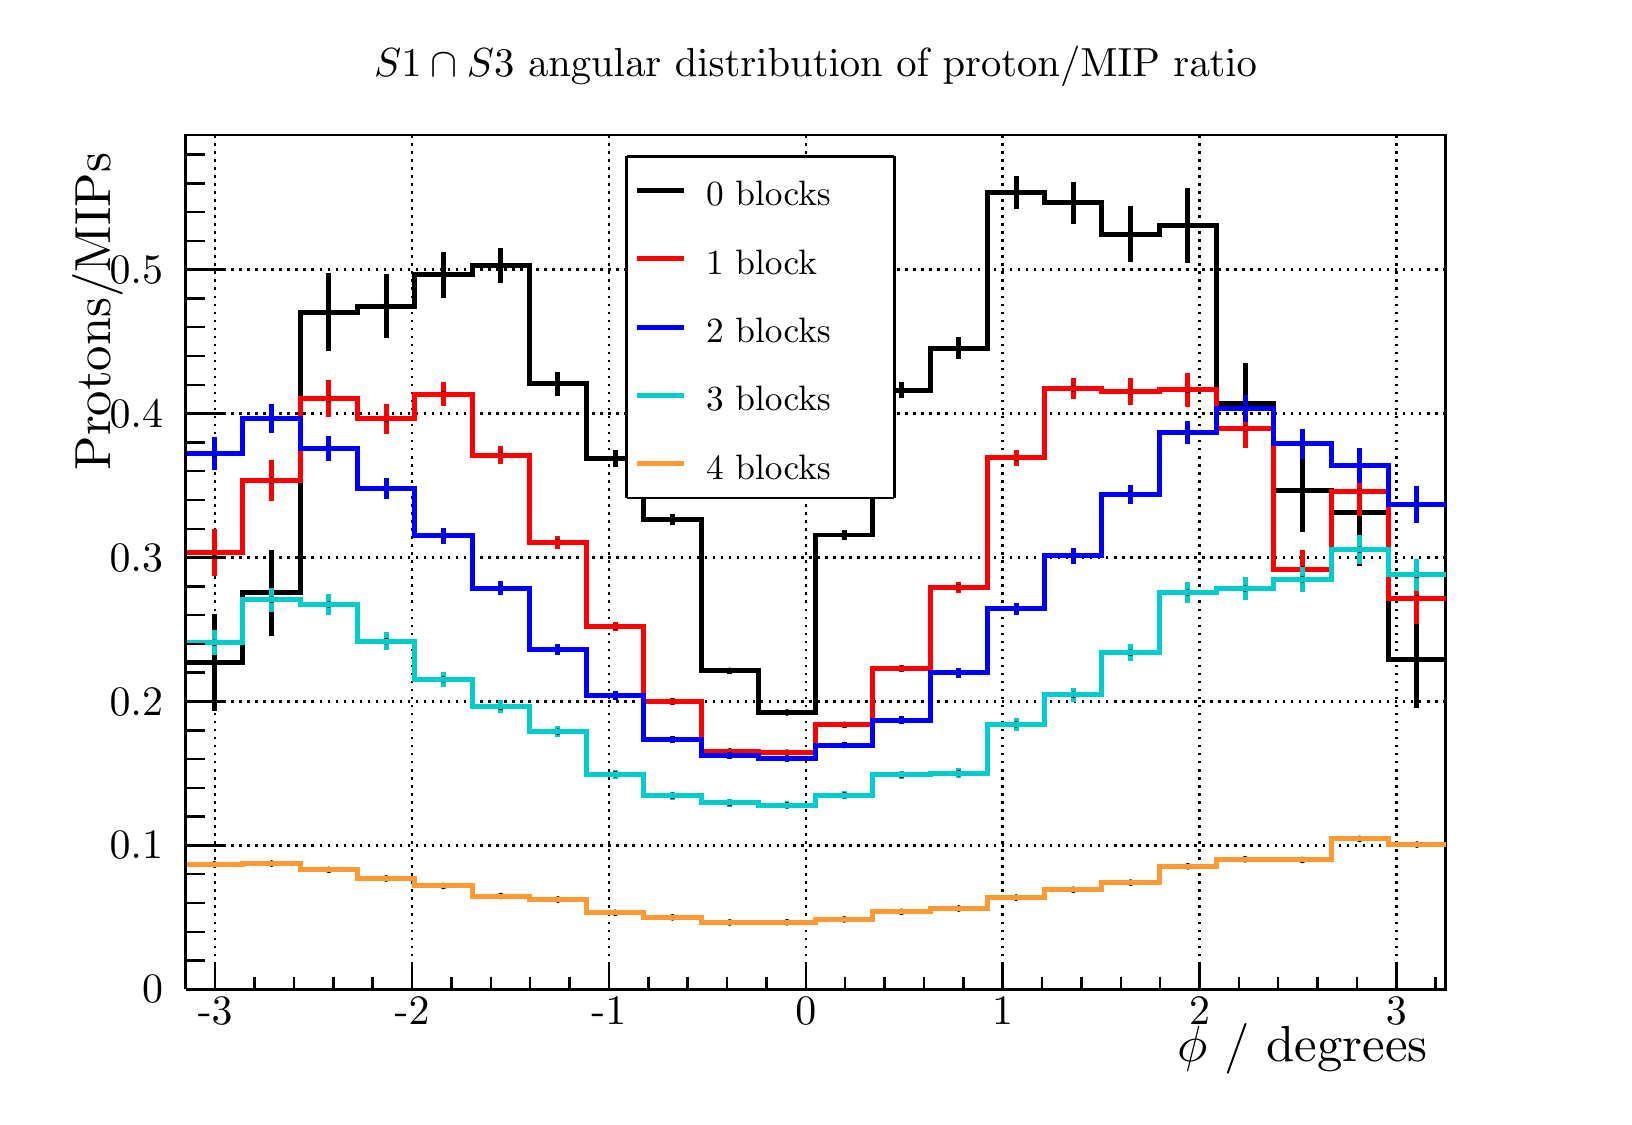
\begin{tikzpicture}
\pgfdeclareplotmark{cross} {
\pgfpathmoveto{\pgfpoint{-0.3\pgfplotmarksize}{\pgfplotmarksize}}
\pgfpathlineto{\pgfpoint{+0.3\pgfplotmarksize}{\pgfplotmarksize}}
\pgfpathlineto{\pgfpoint{+0.3\pgfplotmarksize}{0.3\pgfplotmarksize}}
\pgfpathlineto{\pgfpoint{+1\pgfplotmarksize}{0.3\pgfplotmarksize}}
\pgfpathlineto{\pgfpoint{+1\pgfplotmarksize}{-0.3\pgfplotmarksize}}
\pgfpathlineto{\pgfpoint{+0.3\pgfplotmarksize}{-0.3\pgfplotmarksize}}
\pgfpathlineto{\pgfpoint{+0.3\pgfplotmarksize}{-1.\pgfplotmarksize}}
\pgfpathlineto{\pgfpoint{-0.3\pgfplotmarksize}{-1.\pgfplotmarksize}}
\pgfpathlineto{\pgfpoint{-0.3\pgfplotmarksize}{-0.3\pgfplotmarksize}}
\pgfpathlineto{\pgfpoint{-1.\pgfplotmarksize}{-0.3\pgfplotmarksize}}
\pgfpathlineto{\pgfpoint{-1.\pgfplotmarksize}{0.3\pgfplotmarksize}}
\pgfpathlineto{\pgfpoint{-0.3\pgfplotmarksize}{0.3\pgfplotmarksize}}
\pgfpathclose
\pgfusepathqstroke
}
\pgfdeclareplotmark{cross*} {
\pgfpathmoveto{\pgfpoint{-0.3\pgfplotmarksize}{\pgfplotmarksize}}
\pgfpathlineto{\pgfpoint{+0.3\pgfplotmarksize}{\pgfplotmarksize}}
\pgfpathlineto{\pgfpoint{+0.3\pgfplotmarksize}{0.3\pgfplotmarksize}}
\pgfpathlineto{\pgfpoint{+1\pgfplotmarksize}{0.3\pgfplotmarksize}}
\pgfpathlineto{\pgfpoint{+1\pgfplotmarksize}{-0.3\pgfplotmarksize}}
\pgfpathlineto{\pgfpoint{+0.3\pgfplotmarksize}{-0.3\pgfplotmarksize}}
\pgfpathlineto{\pgfpoint{+0.3\pgfplotmarksize}{-1.\pgfplotmarksize}}
\pgfpathlineto{\pgfpoint{-0.3\pgfplotmarksize}{-1.\pgfplotmarksize}}
\pgfpathlineto{\pgfpoint{-0.3\pgfplotmarksize}{-0.3\pgfplotmarksize}}
\pgfpathlineto{\pgfpoint{-1.\pgfplotmarksize}{-0.3\pgfplotmarksize}}
\pgfpathlineto{\pgfpoint{-1.\pgfplotmarksize}{0.3\pgfplotmarksize}}
\pgfpathlineto{\pgfpoint{-0.3\pgfplotmarksize}{0.3\pgfplotmarksize}}
\pgfpathclose
\pgfusepathqfillstroke
}
\pgfdeclareplotmark{newstar} {
\pgfpathmoveto{\pgfqpoint{0pt}{\pgfplotmarksize}}
\pgfpathlineto{\pgfqpointpolar{44}{0.5\pgfplotmarksize}}
\pgfpathlineto{\pgfqpointpolar{18}{\pgfplotmarksize}}
\pgfpathlineto{\pgfqpointpolar{-20}{0.5\pgfplotmarksize}}
\pgfpathlineto{\pgfqpointpolar{-54}{\pgfplotmarksize}}
\pgfpathlineto{\pgfqpointpolar{-90}{0.5\pgfplotmarksize}}
\pgfpathlineto{\pgfqpointpolar{234}{\pgfplotmarksize}}
\pgfpathlineto{\pgfqpointpolar{198}{0.5\pgfplotmarksize}}
\pgfpathlineto{\pgfqpointpolar{162}{\pgfplotmarksize}}
\pgfpathlineto{\pgfqpointpolar{134}{0.5\pgfplotmarksize}}
\pgfpathclose
\pgfusepathqstroke
}
\pgfdeclareplotmark{newstar*} {
\pgfpathmoveto{\pgfqpoint{0pt}{\pgfplotmarksize}}
\pgfpathlineto{\pgfqpointpolar{44}{0.5\pgfplotmarksize}}
\pgfpathlineto{\pgfqpointpolar{18}{\pgfplotmarksize}}
\pgfpathlineto{\pgfqpointpolar{-20}{0.5\pgfplotmarksize}}
\pgfpathlineto{\pgfqpointpolar{-54}{\pgfplotmarksize}}
\pgfpathlineto{\pgfqpointpolar{-90}{0.5\pgfplotmarksize}}
\pgfpathlineto{\pgfqpointpolar{234}{\pgfplotmarksize}}
\pgfpathlineto{\pgfqpointpolar{198}{0.5\pgfplotmarksize}}
\pgfpathlineto{\pgfqpointpolar{162}{\pgfplotmarksize}}
\pgfpathlineto{\pgfqpointpolar{134}{0.5\pgfplotmarksize}}
\pgfpathclose
\pgfusepathqfillstroke
}
\definecolor{c}{rgb}{1,1,1};
\draw [color=c, fill=c] (0,0) rectangle (20,13.5632);
\draw [color=c, fill=c] (2,1.35632) rectangle (18,12.2069);
\definecolor{c}{rgb}{0,0,0};
\draw [c,line width=0.9] (2,1.35632) -- (2,12.2069) -- (18,12.2069) -- (18,1.35632) -- (2,1.35632);
\definecolor{c}{rgb}{1,1,1};
\draw [color=c, fill=c] (2,1.35632) rectangle (18,12.2069);
\definecolor{c}{rgb}{0,0,0};
\draw [c,line width=0.9] (2,1.35632) -- (2,12.2069) -- (18,12.2069) -- (18,1.35632) -- (2,1.35632);
\draw [c,line width=0.9] (2,1.35632) -- (18,1.35632);
\draw [c,dotted,line width=0.9] (2.375,12.2069) -- (2.375,1.35632);
\draw [c,dotted,line width=0.9] (4.875,12.2069) -- (4.875,1.35632);
\draw [c,dotted,line width=0.9] (7.375,12.2069) -- (7.375,1.35632);
\draw [c,dotted,line width=0.9] (9.875,12.2069) -- (9.875,1.35632);
\draw [c,dotted,line width=0.9] (12.375,12.2069) -- (12.375,1.35632);
\draw [c,dotted,line width=0.9] (14.875,12.2069) -- (14.875,1.35632);
\draw [c,dotted,line width=0.9] (17.375,12.2069) -- (17.375,1.35632);
\draw [c,dotted,line width=0.9] (2.375,12.2069) -- (2.375,1.35632);
\draw [c,dotted,line width=0.9] (17.375,12.2069) -- (17.375,1.35632);
\draw [c,line width=0.9] (2,1.35632) -- (2,12.2069);
\draw [c,dotted,line width=0.9] (18,1.35632) -- (2,1.35632);
\draw [c,dotted,line width=0.9] (18,3.18443) -- (2,3.18443);
\draw [c,dotted,line width=0.9] (18,5.01255) -- (2,5.01255);
\draw [c,dotted,line width=0.9] (18,6.84066) -- (2,6.84066);
\draw [c,dotted,line width=0.9] (18,8.66877) -- (2,8.66877);
\draw [c,dotted,line width=0.9] (18,10.4969) -- (2,10.4969);
\draw [c,dotted,line width=0.9] (18,10.4969) -- (2,10.4969);
\definecolor{c}{rgb}{0,0,0.6};
\draw [c,line width=0.9] (2,1.35632) -- (2.72727,1.35632) -- (2.72727,1.35632) -- (3.45455,1.35632) -- (3.45455,1.35632) -- (4.18182,1.35632) -- (4.18182,1.35632) -- (4.90909,1.35632) -- (4.90909,1.35632) -- (5.63636,1.35632) -- (5.63636,1.35632) --
 (6.36364,1.35632) -- (6.36364,1.35632) -- (7.09091,1.35632) -- (7.09091,1.35632) -- (7.81818,1.35632) -- (7.81818,1.35632) -- (8.54545,1.35632) -- (8.54545,1.35632) -- (9.27273,1.35632) -- (9.27273,1.35632) -- (10,1.35632) -- (10,1.35632) --
 (10.7273,1.35632) -- (10.7273,1.35632) -- (11.4545,1.35632) -- (11.4545,1.35632) -- (12.1818,1.35632) -- (12.1818,1.35632) -- (12.9091,1.35632) -- (12.9091,1.35632) -- (13.6364,1.35632) -- (13.6364,1.35632) -- (14.3636,1.35632) -- (14.3636,1.35632)
 -- (15.0909,1.35632) -- (15.0909,1.35632) -- (15.8182,1.35632) -- (15.8182,1.35632) -- (16.5455,1.35632) -- (16.5455,1.35632) -- (17.2727,1.35632) -- (17.2727,1.35632) -- (18,1.35632);
\definecolor{c}{rgb}{0,0,0};
\draw [c,line width=0.9] (2,1.35632) -- (18,1.35632);
\draw [anchor= east] (18,0.596782) node[scale=1.8317, color=c, rotate=0]{$\phi$ / degrees};
\draw [c,line width=0.9] (2.375,1.68184) -- (2.375,1.35632);
\draw [c,line width=0.9] (2.875,1.51908) -- (2.875,1.35632);
\draw [c,line width=0.9] (3.375,1.51908) -- (3.375,1.35632);
\draw [c,line width=0.9] (3.875,1.51908) -- (3.875,1.35632);
\draw [c,line width=0.9] (4.375,1.51908) -- (4.375,1.35632);
\draw [c,line width=0.9] (4.875,1.68184) -- (4.875,1.35632);
\draw [c,line width=0.9] (5.375,1.51908) -- (5.375,1.35632);
\draw [c,line width=0.9] (5.875,1.51908) -- (5.875,1.35632);
\draw [c,line width=0.9] (6.375,1.51908) -- (6.375,1.35632);
\draw [c,line width=0.9] (6.875,1.51908) -- (6.875,1.35632);
\draw [c,line width=0.9] (7.375,1.68184) -- (7.375,1.35632);
\draw [c,line width=0.9] (7.875,1.51908) -- (7.875,1.35632);
\draw [c,line width=0.9] (8.375,1.51908) -- (8.375,1.35632);
\draw [c,line width=0.9] (8.875,1.51908) -- (8.875,1.35632);
\draw [c,line width=0.9] (9.375,1.51908) -- (9.375,1.35632);
\draw [c,line width=0.9] (9.875,1.68184) -- (9.875,1.35632);
\draw [c,line width=0.9] (10.375,1.51908) -- (10.375,1.35632);
\draw [c,line width=0.9] (10.875,1.51908) -- (10.875,1.35632);
\draw [c,line width=0.9] (11.375,1.51908) -- (11.375,1.35632);
\draw [c,line width=0.9] (11.875,1.51908) -- (11.875,1.35632);
\draw [c,line width=0.9] (12.375,1.68184) -- (12.375,1.35632);
\draw [c,line width=0.9] (12.875,1.51908) -- (12.875,1.35632);
\draw [c,line width=0.9] (13.375,1.51908) -- (13.375,1.35632);
\draw [c,line width=0.9] (13.875,1.51908) -- (13.875,1.35632);
\draw [c,line width=0.9] (14.375,1.51908) -- (14.375,1.35632);
\draw [c,line width=0.9] (14.875,1.68184) -- (14.875,1.35632);
\draw [c,line width=0.9] (15.375,1.51908) -- (15.375,1.35632);
\draw [c,line width=0.9] (15.875,1.51908) -- (15.875,1.35632);
\draw [c,line width=0.9] (16.375,1.51908) -- (16.375,1.35632);
\draw [c,line width=0.9] (16.875,1.51908) -- (16.875,1.35632);
\draw [c,line width=0.9] (17.375,1.68184) -- (17.375,1.35632);
\draw [c,line width=0.9] (2.375,1.68184) -- (2.375,1.35632);
\draw [c,line width=0.9] (17.375,1.68184) -- (17.375,1.35632);
\draw [c,line width=0.9] (17.875,1.51908) -- (17.875,1.35632);
\draw [anchor=base] (2.375,0.908736) node[scale=1.5137, color=c, rotate=0]{-3};
\draw [anchor=base] (4.875,0.908736) node[scale=1.5137, color=c, rotate=0]{-2};
\draw [anchor=base] (7.375,0.908736) node[scale=1.5137, color=c, rotate=0]{-1};
\draw [anchor=base] (9.875,0.908736) node[scale=1.5137, color=c, rotate=0]{0};
\draw [anchor=base] (12.375,0.908736) node[scale=1.5137, color=c, rotate=0]{1};
\draw [anchor=base] (14.875,0.908736) node[scale=1.5137, color=c, rotate=0]{2};
\draw [anchor=base] (17.375,0.908736) node[scale=1.5137, color=c, rotate=0]{3};
\draw [c,line width=0.9] (2,1.35632) -- (2,12.2069);
\draw [anchor= east] (0.88,12.2069) node[scale=1.8317, color=c, rotate=90]{  Protons/MIPs};
\draw [c,line width=0.9] (2.48,1.35632) -- (2,1.35632);
\draw [c,line width=0.9] (2.24,1.72194) -- (2,1.72194);
\draw [c,line width=0.9] (2.24,2.08757) -- (2,2.08757);
\draw [c,line width=0.9] (2.24,2.45319) -- (2,2.45319);
\draw [c,line width=0.9] (2.24,2.81881) -- (2,2.81881);
\draw [c,line width=0.9] (2.48,3.18443) -- (2,3.18443);
\draw [c,line width=0.9] (2.24,3.55006) -- (2,3.55006);
\draw [c,line width=0.9] (2.24,3.91568) -- (2,3.91568);
\draw [c,line width=0.9] (2.24,4.2813) -- (2,4.2813);
\draw [c,line width=0.9] (2.24,4.64692) -- (2,4.64692);
\draw [c,line width=0.9] (2.48,5.01255) -- (2,5.01255);
\draw [c,line width=0.9] (2.24,5.37817) -- (2,5.37817);
\draw [c,line width=0.9] (2.24,5.74379) -- (2,5.74379);
\draw [c,line width=0.9] (2.24,6.10941) -- (2,6.10941);
\draw [c,line width=0.9] (2.24,6.47504) -- (2,6.47504);
\draw [c,line width=0.9] (2.48,6.84066) -- (2,6.84066);
\draw [c,line width=0.9] (2.24,7.20628) -- (2,7.20628);
\draw [c,line width=0.9] (2.24,7.5719) -- (2,7.5719);
\draw [c,line width=0.9] (2.24,7.93753) -- (2,7.93753);
\draw [c,line width=0.9] (2.24,8.30315) -- (2,8.30315);
\draw [c,line width=0.9] (2.48,8.66877) -- (2,8.66877);
\draw [c,line width=0.9] (2.24,9.03439) -- (2,9.03439);
\draw [c,line width=0.9] (2.24,9.40002) -- (2,9.40002);
\draw [c,line width=0.9] (2.24,9.76564) -- (2,9.76564);
\draw [c,line width=0.9] (2.24,10.1313) -- (2,10.1313);
\draw [c,line width=0.9] (2.48,10.4969) -- (2,10.4969);
\draw [c,line width=0.9] (2.48,10.4969) -- (2,10.4969);
\draw [c,line width=0.9] (2.24,10.8625) -- (2,10.8625);
\draw [c,line width=0.9] (2.24,11.2281) -- (2,11.2281);
\draw [c,line width=0.9] (2.24,11.5938) -- (2,11.5938);
\draw [c,line width=0.9] (2.24,11.9594) -- (2,11.9594);
\draw [anchor= east] (1.9,1.35632) node[scale=1.5137, color=c, rotate=0]{0};
\draw [anchor= east] (1.9,3.18443) node[scale=1.5137, color=c, rotate=0]{0.1};
\draw [anchor= east] (1.9,5.01255) node[scale=1.5137, color=c, rotate=0]{0.2};
\draw [anchor= east] (1.9,6.84066) node[scale=1.5137, color=c, rotate=0]{0.3};
\draw [anchor= east] (1.9,8.66877) node[scale=1.5137, color=c, rotate=0]{0.4};
\draw [anchor= east] (1.9,10.4969) node[scale=1.5137, color=c, rotate=0]{0.5};
\draw [c,line width=1.8] (2.36364,4.89378) -- (2.36364,5.51112);
\draw [c,line width=1.8] (2.36364,5.51112) -- (2.36364,6.12847);
\foreach \P in {(2.36364,5.51112)}{\draw[mark options={color=c,fill=c},mark size=2.402402pt,mark=*,mark size=1pt] plot coordinates {\P};}
\draw [c,line width=1.8] (3.09091,5.84926) -- (3.09091,6.39379);
\draw [c,line width=1.8] (3.09091,6.39379) -- (3.09091,6.93831);
\foreach \P in {(3.09091,6.39379)}{\draw[mark options={color=c,fill=c},mark size=2.402402pt,mark=*,mark size=1pt] plot coordinates {\P};}
\draw [c,line width=1.8] (3.81818,9.45971) -- (3.81818,9.95602);
\draw [c,line width=1.8] (3.81818,9.95602) -- (3.81818,10.4523);
\foreach \P in {(3.81818,9.95602)}{\draw[mark options={color=c,fill=c},mark size=2.402402pt,mark=*,mark size=1pt] plot coordinates {\P};}
\draw [c,line width=1.8] (4.54545,9.62928) -- (4.54545,10.0327);
\draw [c,line width=1.8] (4.54545,10.0327) -- (4.54545,10.4362);
\foreach \P in {(4.54545,10.0327)}{\draw[mark options={color=c,fill=c},mark size=2.402402pt,mark=*,mark size=1pt] plot coordinates {\P};}
\draw [c,line width=1.8] (5.27273,10.1359) -- (5.27273,10.4304);
\draw [c,line width=1.8] (5.27273,10.4304) -- (5.27273,10.725);
\foreach \P in {(5.27273,10.4304)}{\draw[mark options={color=c,fill=c},mark size=2.402402pt,mark=*,mark size=1pt] plot coordinates {\P};}
\draw [c,line width=1.8] (6,10.3215) -- (6,10.547);
\draw [c,line width=1.8] (6,10.547) -- (6,10.7725);
\foreach \P in {(6,10.547)}{\draw[mark options={color=c,fill=c},mark size=2.402402pt,mark=*,mark size=1pt] plot coordinates {\P};}
\draw [c,line width=1.8] (6.72727,8.89213) -- (6.72727,9.04764);
\draw [c,line width=1.8] (6.72727,9.04764) -- (6.72727,9.20315);
\foreach \P in {(6.72727,9.04764)}{\draw[mark options={color=c,fill=c},mark size=2.402402pt,mark=*,mark size=1pt] plot coordinates {\P};}
\draw [c,line width=1.8] (7.45455,7.99309) -- (7.45455,8.09945);
\draw [c,line width=1.8] (7.45455,8.09945) -- (7.45455,8.2058);
\foreach \P in {(7.45455,8.09945)}{\draw[mark options={color=c,fill=c},mark size=2.402402pt,mark=*,mark size=1pt] plot coordinates {\P};}
\draw [c,line width=1.8] (8.18182,7.25752) -- (8.18182,7.3273);
\draw [c,line width=1.8] (8.18182,7.3273) -- (8.18182,7.39708);
\foreach \P in {(8.18182,7.3273)}{\draw[mark options={color=c,fill=c},mark size=2.402402pt,mark=*,mark size=1pt] plot coordinates {\P};}
\draw [c,line width=1.8] (8.90909,5.36598) -- (8.90909,5.40179);
\draw [c,line width=1.8] (8.90909,5.40179) -- (8.90909,5.4376);
\foreach \P in {(8.90909,5.40179)}{\draw[mark options={color=c,fill=c},mark size=2.402402pt,mark=*,mark size=1pt] plot coordinates {\P};}
\draw [c,line width=1.8] (9.63636,4.84341) -- (9.63636,4.87303);
\draw [c,line width=1.8] (9.63636,4.87303) -- (9.63636,4.90264);
\foreach \P in {(9.63636,4.87303)}{\draw[mark options={color=c,fill=c},mark size=2.402402pt,mark=*,mark size=1pt] plot coordinates {\P};}
\draw [c,line width=1.8] (10.3636,7.06938) -- (10.3636,7.12713);
\draw [c,line width=1.8] (10.3636,7.12713) -- (10.3636,7.18488);
\foreach \P in {(10.3636,7.12713)}{\draw[mark options={color=c,fill=c},mark size=2.402402pt,mark=*,mark size=1pt] plot coordinates {\P};}
\draw [c,line width=1.8] (11.0909,8.86292) -- (11.0909,8.96454);
\draw [c,line width=1.8] (11.0909,8.96454) -- (11.0909,9.06617);
\foreach \P in {(11.0909,8.96454)}{\draw[mark options={color=c,fill=c},mark size=2.402402pt,mark=*,mark size=1pt] plot coordinates {\P};}
\draw [c,line width=1.8] (11.8182,9.36011) -- (11.8182,9.50073);
\draw [c,line width=1.8] (11.8182,9.50073) -- (11.8182,9.64135);
\foreach \P in {(11.8182,9.50073)}{\draw[mark options={color=c,fill=c},mark size=2.402402pt,mark=*,mark size=1pt] plot coordinates {\P};}
\draw [c,line width=1.8] (12.5455,11.263) -- (12.5455,11.4766);
\draw [c,line width=1.8] (12.5455,11.4766) -- (12.5455,11.6902);
\foreach \P in {(12.5455,11.4766)}{\draw[mark options={color=c,fill=c},mark size=2.402402pt,mark=*,mark size=1pt] plot coordinates {\P};}
\draw [c,line width=1.8] (13.2727,11.0759) -- (13.2727,11.3437);
\draw [c,line width=1.8] (13.2727,11.3437) -- (13.2727,11.6115);
\foreach \P in {(13.2727,11.3437)}{\draw[mark options={color=c,fill=c},mark size=2.402402pt,mark=*,mark size=1pt] plot coordinates {\P};}
\draw [c,line width=1.8] (14,10.588) -- (14,10.9455);
\draw [c,line width=1.8] (14,10.9455) -- (14,11.303);
\foreach \P in {(14,10.9455)}{\draw[mark options={color=c,fill=c},mark size=2.402402pt,mark=*,mark size=1pt] plot coordinates {\P};}
\draw [c,line width=1.8] (14.7273,10.5864) -- (14.7273,11.0575);
\draw [c,line width=1.8] (14.7273,11.0575) -- (14.7273,11.5286);
\foreach \P in {(14.7273,11.0575)}{\draw[mark options={color=c,fill=c},mark size=2.402402pt,mark=*,mark size=1pt] plot coordinates {\P};}
\draw [c,line width=1.8] (15.4545,8.28922) -- (15.4545,8.79768);
\draw [c,line width=1.8] (15.4545,8.79768) -- (15.4545,9.30614);
\foreach \P in {(15.4545,8.79768)}{\draw[mark options={color=c,fill=c},mark size=2.402402pt,mark=*,mark size=1pt] plot coordinates {\P};}
\draw [c,line width=1.8] (16.1818,7.16906) -- (16.1818,7.69467);
\draw [c,line width=1.8] (16.1818,7.69467) -- (16.1818,8.22028);
\foreach \P in {(16.1818,7.69467)}{\draw[mark options={color=c,fill=c},mark size=2.402402pt,mark=*,mark size=1pt] plot coordinates {\P};}
\draw [c,line width=1.8] (16.9091,6.73172) -- (16.9091,7.41194);
\draw [c,line width=1.8] (16.9091,7.41194) -- (16.9091,8.09217);
\foreach \P in {(16.9091,7.41194)}{\draw[mark options={color=c,fill=c},mark size=2.402402pt,mark=*,mark size=1pt] plot coordinates {\P};}
\draw [c,line width=1.8] (17.6364,4.93484) -- (17.6364,5.54817);
\draw [c,line width=1.8] (17.6364,5.54817) -- (17.6364,6.16151);
\foreach \P in {(17.6364,5.54817)}{\draw[mark options={color=c,fill=c},mark size=2.402402pt,mark=*,mark size=1pt] plot coordinates {\P};}
\draw [c,line width=1.8] (2,5.51112) -- (2.72727,5.51112) -- (2.72727,6.39379) -- (3.45455,6.39379) -- (3.45455,9.95602) -- (4.18182,9.95602) -- (4.18182,10.0327) -- (4.90909,10.0327) -- (4.90909,10.4304) -- (5.63636,10.4304) -- (5.63636,10.547) --
 (6.36364,10.547) -- (6.36364,9.04764) -- (7.09091,9.04764) -- (7.09091,8.09945) -- (7.81818,8.09945) -- (7.81818,7.3273) -- (8.54545,7.3273) -- (8.54545,5.40179) -- (9.27273,5.40179) -- (9.27273,4.87303) -- (10,4.87303) -- (10,7.12713) --
 (10.7273,7.12713) -- (10.7273,8.96454) -- (11.4545,8.96454) -- (11.4545,9.50073) -- (12.1818,9.50073) -- (12.1818,11.4766) -- (12.9091,11.4766) -- (12.9091,11.3437) -- (13.6364,11.3437) -- (13.6364,10.9455) -- (14.3636,10.9455) -- (14.3636,11.0575)
 -- (15.0909,11.0575) -- (15.0909,8.79768) -- (15.8182,8.79768) -- (15.8182,7.69467) -- (16.5455,7.69467) -- (16.5455,7.41194) -- (17.2727,7.41194) -- (17.2727,5.54817) -- (18,5.54817);
\definecolor{c}{rgb}{1,0,0};
\draw [c,line width=1.8] (2.36364,6.60423) -- (2.36364,6.90306);
\draw [c,line width=1.8] (2.36364,6.90306) -- (2.36364,7.20189);
\definecolor{c}{rgb}{0,0,0};
\foreach \P in {(2.36364,6.90306)}{\draw[mark options={color=c,fill=c},mark size=2.402402pt,mark=*,mark size=1pt] plot coordinates {\P};}
\definecolor{c}{rgb}{1,0,0};
\draw [c,line width=1.8] (3.09091,7.5545) -- (3.09091,7.8162);
\draw [c,line width=1.8] (3.09091,7.8162) -- (3.09091,8.0779);
\definecolor{c}{rgb}{0,0,0};
\foreach \P in {(3.09091,7.8162)}{\draw[mark options={color=c,fill=c},mark size=2.402402pt,mark=*,mark size=1pt] plot coordinates {\P};}
\definecolor{c}{rgb}{1,0,0};
\draw [c,line width=1.8] (3.81818,8.62873) -- (3.81818,8.86031);
\draw [c,line width=1.8] (3.81818,8.86031) -- (3.81818,9.09189);
\definecolor{c}{rgb}{0,0,0};
\foreach \P in {(3.81818,8.86031)}{\draw[mark options={color=c,fill=c},mark size=2.402402pt,mark=*,mark size=1pt] plot coordinates {\P};}
\definecolor{c}{rgb}{1,0,0};
\draw [c,line width=1.8] (4.54545,8.41495) -- (4.54545,8.60083);
\draw [c,line width=1.8] (4.54545,8.60083) -- (4.54545,8.78671);
\definecolor{c}{rgb}{0,0,0};
\foreach \P in {(4.54545,8.60083)}{\draw[mark options={color=c,fill=c},mark size=2.402402pt,mark=*,mark size=1pt] plot coordinates {\P};}
\definecolor{c}{rgb}{1,0,0};
\draw [c,line width=1.8] (5.27273,8.76828) -- (5.27273,8.91648);
\draw [c,line width=1.8] (5.27273,8.91648) -- (5.27273,9.06469);
\definecolor{c}{rgb}{0,0,0};
\foreach \P in {(5.27273,8.91648)}{\draw[mark options={color=c,fill=c},mark size=2.402402pt,mark=*,mark size=1pt] plot coordinates {\P};}
\definecolor{c}{rgb}{1,0,0};
\draw [c,line width=1.8] (6,8.02779) -- (6,8.14192);
\draw [c,line width=1.8] (6,8.14192) -- (6,8.25604);
\definecolor{c}{rgb}{0,0,0};
\foreach \P in {(6,8.14192)}{\draw[mark options={color=c,fill=c},mark size=2.402402pt,mark=*,mark size=1pt] plot coordinates {\P};}
\definecolor{c}{rgb}{1,0,0};
\draw [c,line width=1.8] (6.72727,6.95442) -- (6.72727,7.03619);
\draw [c,line width=1.8] (6.72727,7.03619) -- (6.72727,7.11796);
\definecolor{c}{rgb}{0,0,0};
\foreach \P in {(6.72727,7.03619)}{\draw[mark options={color=c,fill=c},mark size=2.402402pt,mark=*,mark size=1pt] plot coordinates {\P};}
\definecolor{c}{rgb}{1,0,0};
\draw [c,line width=1.8] (7.45455,5.90288) -- (7.45455,5.96141);
\draw [c,line width=1.8] (7.45455,5.96141) -- (7.45455,6.01994);
\definecolor{c}{rgb}{0,0,0};
\foreach \P in {(7.45455,5.96141)}{\draw[mark options={color=c,fill=c},mark size=2.402402pt,mark=*,mark size=1pt] plot coordinates {\P};}
\definecolor{c}{rgb}{1,0,0};
\draw [c,line width=1.8] (8.18182,4.97126) -- (8.18182,5.01446);
\draw [c,line width=1.8] (8.18182,5.01446) -- (8.18182,5.05766);
\definecolor{c}{rgb}{0,0,0};
\foreach \P in {(8.18182,5.01446)}{\draw[mark options={color=c,fill=c},mark size=2.402402pt,mark=*,mark size=1pt] plot coordinates {\P};}
\definecolor{c}{rgb}{1,0,0};
\draw [c,line width=1.8] (8.90909,4.34427) -- (8.90909,4.37898);
\draw [c,line width=1.8] (8.90909,4.37898) -- (8.90909,4.41369);
\definecolor{c}{rgb}{0,0,0};
\foreach \P in {(8.90909,4.37898)}{\draw[mark options={color=c,fill=c},mark size=2.402402pt,mark=*,mark size=1pt] plot coordinates {\P};}
\definecolor{c}{rgb}{1,0,0};
\draw [c,line width=1.8] (9.63636,4.32923) -- (9.63636,4.3633);
\draw [c,line width=1.8] (9.63636,4.3633) -- (9.63636,4.39736);
\definecolor{c}{rgb}{0,0,0};
\foreach \P in {(9.63636,4.3633)}{\draw[mark options={color=c,fill=c},mark size=2.402402pt,mark=*,mark size=1pt] plot coordinates {\P};}
\definecolor{c}{rgb}{1,0,0};
\draw [c,line width=1.8] (10.3636,4.67726) -- (10.3636,4.71602);
\draw [c,line width=1.8] (10.3636,4.71602) -- (10.3636,4.75479);
\definecolor{c}{rgb}{0,0,0};
\foreach \P in {(10.3636,4.71602)}{\draw[mark options={color=c,fill=c},mark size=2.402402pt,mark=*,mark size=1pt] plot coordinates {\P};}
\definecolor{c}{rgb}{1,0,0};
\draw [c,line width=1.8] (11.0909,5.38166) -- (11.0909,5.43154);
\draw [c,line width=1.8] (11.0909,5.43154) -- (11.0909,5.48143);
\definecolor{c}{rgb}{0,0,0};
\foreach \P in {(11.0909,5.43154)}{\draw[mark options={color=c,fill=c},mark size=2.402402pt,mark=*,mark size=1pt] plot coordinates {\P};}
\definecolor{c}{rgb}{1,0,0};
\draw [c,line width=1.8] (11.8182,6.39514) -- (11.8182,6.46287);
\draw [c,line width=1.8] (11.8182,6.46287) -- (11.8182,6.5306);
\definecolor{c}{rgb}{0,0,0};
\foreach \P in {(11.8182,6.46287)}{\draw[mark options={color=c,fill=c},mark size=2.402402pt,mark=*,mark size=1pt] plot coordinates {\P};}
\definecolor{c}{rgb}{1,0,0};
\draw [c,line width=1.8] (12.5455,8.00437) -- (12.5455,8.10677);
\draw [c,line width=1.8] (12.5455,8.10677) -- (12.5455,8.20917);
\definecolor{c}{rgb}{0,0,0};
\foreach \P in {(12.5455,8.10677)}{\draw[mark options={color=c,fill=c},mark size=2.402402pt,mark=*,mark size=1pt] plot coordinates {\P};}
\definecolor{c}{rgb}{1,0,0};
\draw [c,line width=1.8] (13.2727,8.85335) -- (13.2727,8.98853);
\draw [c,line width=1.8] (13.2727,8.98853) -- (13.2727,9.1237);
\definecolor{c}{rgb}{0,0,0};
\foreach \P in {(13.2727,8.98853)}{\draw[mark options={color=c,fill=c},mark size=2.402402pt,mark=*,mark size=1pt] plot coordinates {\P};}
\definecolor{c}{rgb}{1,0,0};
\draw [c,line width=1.8] (14,8.77802) -- (14,8.94714);
\draw [c,line width=1.8] (14,8.94714) -- (14,9.11627);
\definecolor{c}{rgb}{0,0,0};
\foreach \P in {(14,8.94714)}{\draw[mark options={color=c,fill=c},mark size=2.402402pt,mark=*,mark size=1pt] plot coordinates {\P};}
\definecolor{c}{rgb}{1,0,0};
\draw [c,line width=1.8] (14.7273,8.75518) -- (14.7273,8.96999);
\draw [c,line width=1.8] (14.7273,8.96999) -- (14.7273,9.18481);
\definecolor{c}{rgb}{0,0,0};
\foreach \P in {(14.7273,8.96999)}{\draw[mark options={color=c,fill=c},mark size=2.402402pt,mark=*,mark size=1pt] plot coordinates {\P};}
\definecolor{c}{rgb}{1,0,0};
\draw [c,line width=1.8] (15.4545,8.23655) -- (15.4545,8.47919);
\draw [c,line width=1.8] (15.4545,8.47919) -- (15.4545,8.72183);
\definecolor{c}{rgb}{0,0,0};
\foreach \P in {(15.4545,8.47919)}{\draw[mark options={color=c,fill=c},mark size=2.402402pt,mark=*,mark size=1pt] plot coordinates {\P};}
\definecolor{c}{rgb}{1,0,0};
\draw [c,line width=1.8] (16.1818,6.44051) -- (16.1818,6.69109);
\draw [c,line width=1.8] (16.1818,6.69109) -- (16.1818,6.94166);
\definecolor{c}{rgb}{0,0,0};
\foreach \P in {(16.1818,6.69109)}{\draw[mark options={color=c,fill=c},mark size=2.402402pt,mark=*,mark size=1pt] plot coordinates {\P};}
\definecolor{c}{rgb}{1,0,0};
\draw [c,line width=1.8] (16.9091,7.36681) -- (16.9091,7.68164);
\draw [c,line width=1.8] (16.9091,7.68164) -- (16.9091,7.99646);
\definecolor{c}{rgb}{0,0,0};
\foreach \P in {(16.9091,7.68164)}{\draw[mark options={color=c,fill=c},mark size=2.402402pt,mark=*,mark size=1pt] plot coordinates {\P};}
\definecolor{c}{rgb}{1,0,0};
\draw [c,line width=1.8] (17.6364,5.99877) -- (17.6364,6.32595);
\draw [c,line width=1.8] (17.6364,6.32595) -- (17.6364,6.65312);
\definecolor{c}{rgb}{0,0,0};
\foreach \P in {(17.6364,6.32595)}{\draw[mark options={color=c,fill=c},mark size=2.402402pt,mark=*,mark size=1pt] plot coordinates {\P};}
\definecolor{c}{rgb}{1,0,0};
\draw [c,line width=1.8] (2,6.90306) -- (2.72727,6.90306) -- (2.72727,7.8162) -- (3.45455,7.8162) -- (3.45455,8.86031) -- (4.18182,8.86031) -- (4.18182,8.60083) -- (4.90909,8.60083) -- (4.90909,8.91648) -- (5.63636,8.91648) -- (5.63636,8.14192) --
 (6.36364,8.14192) -- (6.36364,7.03619) -- (7.09091,7.03619) -- (7.09091,5.96141) -- (7.81818,5.96141) -- (7.81818,5.01446) -- (8.54545,5.01446) -- (8.54545,4.37898) -- (9.27273,4.37898) -- (9.27273,4.3633) -- (10,4.3633) -- (10,4.71602) --
 (10.7273,4.71602) -- (10.7273,5.43154) -- (11.4545,5.43154) -- (11.4545,6.46287) -- (12.1818,6.46287) -- (12.1818,8.10677) -- (12.9091,8.10677) -- (12.9091,8.98853) -- (13.6364,8.98853) -- (13.6364,8.94714) -- (14.3636,8.94714) -- (14.3636,8.96999)
 -- (15.0909,8.96999) -- (15.0909,8.47919) -- (15.8182,8.47919) -- (15.8182,6.69109) -- (16.5455,6.69109) -- (16.5455,7.68164) -- (17.2727,7.68164) -- (17.2727,6.32595) -- (18,6.32595);
\definecolor{c}{rgb}{0,0,1};
\draw [c,line width=1.8] (2.36364,7.94927) -- (2.36364,8.15813);
\draw [c,line width=1.8] (2.36364,8.15813) -- (2.36364,8.36698);
\definecolor{c}{rgb}{0,0,0};
\foreach \P in {(2.36364,8.15813)}{\draw[mark options={color=c,fill=c},mark size=2.402402pt,mark=*,mark size=1pt] plot coordinates {\P};}
\definecolor{c}{rgb}{0,0,1};
\draw [c,line width=1.8] (3.09091,8.41768) -- (3.09091,8.60289);
\draw [c,line width=1.8] (3.09091,8.60289) -- (3.09091,8.78811);
\definecolor{c}{rgb}{0,0,0};
\foreach \P in {(3.09091,8.60289)}{\draw[mark options={color=c,fill=c},mark size=2.402402pt,mark=*,mark size=1pt] plot coordinates {\P};}
\definecolor{c}{rgb}{0,0,1};
\draw [c,line width=1.8] (3.81818,8.07214) -- (3.81818,8.23082);
\draw [c,line width=1.8] (3.81818,8.23082) -- (3.81818,8.38951);
\definecolor{c}{rgb}{0,0,0};
\foreach \P in {(3.81818,8.23082)}{\draw[mark options={color=c,fill=c},mark size=2.402402pt,mark=*,mark size=1pt] plot coordinates {\P};}
\definecolor{c}{rgb}{0,0,1};
\draw [c,line width=1.8] (4.54545,7.58374) -- (4.54545,7.71608);
\draw [c,line width=1.8] (4.54545,7.71608) -- (4.54545,7.84841);
\definecolor{c}{rgb}{0,0,0};
\foreach \P in {(4.54545,7.71608)}{\draw[mark options={color=c,fill=c},mark size=2.402402pt,mark=*,mark size=1pt] plot coordinates {\P};}
\definecolor{c}{rgb}{0,0,1};
\draw [c,line width=1.8] (5.27273,7.0098) -- (5.27273,7.11593);
\draw [c,line width=1.8] (5.27273,7.11593) -- (5.27273,7.22207);
\definecolor{c}{rgb}{0,0,0};
\foreach \P in {(5.27273,7.11593)}{\draw[mark options={color=c,fill=c},mark size=2.402402pt,mark=*,mark size=1pt] plot coordinates {\P};}
\definecolor{c}{rgb}{0,0,1};
\draw [c,line width=1.8] (6,6.36486) -- (6,6.45215);
\draw [c,line width=1.8] (6,6.45215) -- (6,6.53944);
\definecolor{c}{rgb}{0,0,0};
\foreach \P in {(6,6.45215)}{\draw[mark options={color=c,fill=c},mark size=2.402402pt,mark=*,mark size=1pt] plot coordinates {\P};}
\definecolor{c}{rgb}{0,0,1};
\draw [c,line width=1.8] (6.72727,5.60459) -- (6.72727,5.67248);
\draw [c,line width=1.8] (6.72727,5.67248) -- (6.72727,5.74038);
\definecolor{c}{rgb}{0,0,0};
\foreach \P in {(6.72727,5.67248)}{\draw[mark options={color=c,fill=c},mark size=2.402402pt,mark=*,mark size=1pt] plot coordinates {\P};}
\definecolor{c}{rgb}{0,0,1};
\draw [c,line width=1.8] (7.45455,5.03204) -- (7.45455,5.08687);
\draw [c,line width=1.8] (7.45455,5.08687) -- (7.45455,5.14171);
\definecolor{c}{rgb}{0,0,0};
\foreach \P in {(7.45455,5.08687)}{\draw[mark options={color=c,fill=c},mark size=2.402402pt,mark=*,mark size=1pt] plot coordinates {\P};}
\definecolor{c}{rgb}{0,0,1};
\draw [c,line width=1.8] (8.18182,4.4863) -- (8.18182,4.53181);
\draw [c,line width=1.8] (8.18182,4.53181) -- (8.18182,4.57731);
\definecolor{c}{rgb}{0,0,0};
\foreach \P in {(8.18182,4.53181)}{\draw[mark options={color=c,fill=c},mark size=2.402402pt,mark=*,mark size=1pt] plot coordinates {\P};}
\definecolor{c}{rgb}{0,0,1};
\draw [c,line width=1.8] (8.90909,4.287) -- (8.90909,4.32814);
\draw [c,line width=1.8] (8.90909,4.32814) -- (8.90909,4.36928);
\definecolor{c}{rgb}{0,0,0};
\foreach \P in {(8.90909,4.32814)}{\draw[mark options={color=c,fill=c},mark size=2.402402pt,mark=*,mark size=1pt] plot coordinates {\P};}
\definecolor{c}{rgb}{0,0,1};
\draw [c,line width=1.8] (9.63636,4.24632) -- (9.63636,4.28747);
\draw [c,line width=1.8] (9.63636,4.28747) -- (9.63636,4.32862);
\definecolor{c}{rgb}{0,0,0};
\foreach \P in {(9.63636,4.28747)}{\draw[mark options={color=c,fill=c},mark size=2.402402pt,mark=*,mark size=1pt] plot coordinates {\P};}
\definecolor{c}{rgb}{0,0,1};
\draw [c,line width=1.8] (10.3636,4.41574) -- (10.3636,4.45963);
\draw [c,line width=1.8] (10.3636,4.45963) -- (10.3636,4.50353);
\definecolor{c}{rgb}{0,0,0};
\foreach \P in {(10.3636,4.45963)}{\draw[mark options={color=c,fill=c},mark size=2.402402pt,mark=*,mark size=1pt] plot coordinates {\P};}
\definecolor{c}{rgb}{0,0,1};
\draw [c,line width=1.8] (11.0909,4.72467) -- (11.0909,4.77477);
\draw [c,line width=1.8] (11.0909,4.77477) -- (11.0909,4.82488);
\definecolor{c}{rgb}{0,0,0};
\foreach \P in {(11.0909,4.77477)}{\draw[mark options={color=c,fill=c},mark size=2.402402pt,mark=*,mark size=1pt] plot coordinates {\P};}
\definecolor{c}{rgb}{0,0,1};
\draw [c,line width=1.8] (11.8182,5.31697) -- (11.8182,5.37768);
\draw [c,line width=1.8] (11.8182,5.37768) -- (11.8182,5.43838);
\definecolor{c}{rgb}{0,0,0};
\foreach \P in {(11.8182,5.37768)}{\draw[mark options={color=c,fill=c},mark size=2.402402pt,mark=*,mark size=1pt] plot coordinates {\P};}
\definecolor{c}{rgb}{0,0,1};
\draw [c,line width=1.8] (12.5455,6.10984) -- (12.5455,6.18951);
\draw [c,line width=1.8] (12.5455,6.18951) -- (12.5455,6.26918);
\definecolor{c}{rgb}{0,0,0};
\foreach \P in {(12.5455,6.18951)}{\draw[mark options={color=c,fill=c},mark size=2.402402pt,mark=*,mark size=1pt] plot coordinates {\P};}
\definecolor{c}{rgb}{0,0,1};
\draw [c,line width=1.8] (13.2727,6.76253) -- (13.2727,6.862);
\draw [c,line width=1.8] (13.2727,6.862) -- (13.2727,6.96147);
\definecolor{c}{rgb}{0,0,0};
\foreach \P in {(13.2727,6.862)}{\draw[mark options={color=c,fill=c},mark size=2.402402pt,mark=*,mark size=1pt] plot coordinates {\P};}
\definecolor{c}{rgb}{0,0,1};
\draw [c,line width=1.8] (14,7.52013) -- (14,7.64309);
\draw [c,line width=1.8] (14,7.64309) -- (14,7.76606);
\definecolor{c}{rgb}{0,0,0};
\foreach \P in {(14,7.64309)}{\draw[mark options={color=c,fill=c},mark size=2.402402pt,mark=*,mark size=1pt] plot coordinates {\P};}
\definecolor{c}{rgb}{0,0,1};
\draw [c,line width=1.8] (14.7273,8.27652) -- (14.7273,8.42762);
\draw [c,line width=1.8] (14.7273,8.42762) -- (14.7273,8.57872);
\definecolor{c}{rgb}{0,0,0};
\foreach \P in {(14.7273,8.42762)}{\draw[mark options={color=c,fill=c},mark size=2.402402pt,mark=*,mark size=1pt] plot coordinates {\P};}
\definecolor{c}{rgb}{0,0,1};
\draw [c,line width=1.8] (15.4545,8.56516) -- (15.4545,8.73804);
\draw [c,line width=1.8] (15.4545,8.73804) -- (15.4545,8.91092);
\definecolor{c}{rgb}{0,0,0};
\foreach \P in {(15.4545,8.73804)}{\draw[mark options={color=c,fill=c},mark size=2.402402pt,mark=*,mark size=1pt] plot coordinates {\P};}
\definecolor{c}{rgb}{0,0,1};
\draw [c,line width=1.8] (16.1818,8.09282) -- (16.1818,8.28382);
\draw [c,line width=1.8] (16.1818,8.28382) -- (16.1818,8.47482);
\definecolor{c}{rgb}{0,0,0};
\foreach \P in {(16.1818,8.28382)}{\draw[mark options={color=c,fill=c},mark size=2.402402pt,mark=*,mark size=1pt] plot coordinates {\P};}
\definecolor{c}{rgb}{0,0,1};
\draw [c,line width=1.8] (16.9091,7.78327) -- (16.9091,8.00724);
\draw [c,line width=1.8] (16.9091,8.00724) -- (16.9091,8.23121);
\definecolor{c}{rgb}{0,0,0};
\foreach \P in {(16.9091,8.00724)}{\draw[mark options={color=c,fill=c},mark size=2.402402pt,mark=*,mark size=1pt] plot coordinates {\P};}
\definecolor{c}{rgb}{0,0,1};
\draw [c,line width=1.8] (17.6364,7.27676) -- (17.6364,7.51476);
\draw [c,line width=1.8] (17.6364,7.51476) -- (17.6364,7.75276);
\definecolor{c}{rgb}{0,0,0};
\foreach \P in {(17.6364,7.51476)}{\draw[mark options={color=c,fill=c},mark size=2.402402pt,mark=*,mark size=1pt] plot coordinates {\P};}
\definecolor{c}{rgb}{0,0,1};
\draw [c,line width=1.8] (2,8.15813) -- (2.72727,8.15813) -- (2.72727,8.60289) -- (3.45455,8.60289) -- (3.45455,8.23082) -- (4.18182,8.23082) -- (4.18182,7.71608) -- (4.90909,7.71608) -- (4.90909,7.11593) -- (5.63636,7.11593) -- (5.63636,6.45215) --
 (6.36364,6.45215) -- (6.36364,5.67248) -- (7.09091,5.67248) -- (7.09091,5.08687) -- (7.81818,5.08687) -- (7.81818,4.53181) -- (8.54545,4.53181) -- (8.54545,4.32814) -- (9.27273,4.32814) -- (9.27273,4.28747) -- (10,4.28747) -- (10,4.45963) --
 (10.7273,4.45963) -- (10.7273,4.77477) -- (11.4545,4.77477) -- (11.4545,5.37768) -- (12.1818,5.37768) -- (12.1818,6.18951) -- (12.9091,6.18951) -- (12.9091,6.862) -- (13.6364,6.862) -- (13.6364,7.64309) -- (14.3636,7.64309) -- (14.3636,8.42762) --
 (15.0909,8.42762) -- (15.0909,8.73804) -- (15.8182,8.73804) -- (15.8182,8.28382) -- (16.5455,8.28382) -- (16.5455,8.00724) -- (17.2727,8.00724) -- (17.2727,7.51476) -- (18,7.51476);
\definecolor{c}{rgb}{0,0.8,0.8};
\draw [c,line width=1.8] (2.36364,5.60065) -- (2.36364,5.75802);
\draw [c,line width=1.8] (2.36364,5.75802) -- (2.36364,5.91539);
\definecolor{c}{rgb}{0,0,0};
\foreach \P in {(2.36364,5.75802)}{\draw[mark options={color=c,fill=c},mark size=2.402402pt,mark=*,mark size=1pt] plot coordinates {\P};}
\definecolor{c}{rgb}{0,0.8,0.8};
\draw [c,line width=1.8] (3.09091,6.15354) -- (3.09091,6.30546);
\draw [c,line width=1.8] (3.09091,6.30546) -- (3.09091,6.45738);
\definecolor{c}{rgb}{0,0,0};
\foreach \P in {(3.09091,6.30546)}{\draw[mark options={color=c,fill=c},mark size=2.402402pt,mark=*,mark size=1pt] plot coordinates {\P};}
\definecolor{c}{rgb}{0,0.8,0.8};
\draw [c,line width=1.8] (3.81818,6.10854) -- (3.81818,6.24391);
\draw [c,line width=1.8] (3.81818,6.24391) -- (3.81818,6.37929);
\definecolor{c}{rgb}{0,0,0};
\foreach \P in {(3.81818,6.24391)}{\draw[mark options={color=c,fill=c},mark size=2.402402pt,mark=*,mark size=1pt] plot coordinates {\P};}
\definecolor{c}{rgb}{0,0.8,0.8};
\draw [c,line width=1.8] (4.54545,5.66395) -- (4.54545,5.77943);
\draw [c,line width=1.8] (4.54545,5.77943) -- (4.54545,5.89492);
\definecolor{c}{rgb}{0,0,0};
\foreach \P in {(4.54545,5.77943)}{\draw[mark options={color=c,fill=c},mark size=2.402402pt,mark=*,mark size=1pt] plot coordinates {\P};}
\definecolor{c}{rgb}{0,0.8,0.8};
\draw [c,line width=1.8] (5.27273,5.1981) -- (5.27273,5.29348);
\draw [c,line width=1.8] (5.27273,5.29348) -- (5.27273,5.38886);
\definecolor{c}{rgb}{0,0,0};
\foreach \P in {(5.27273,5.29348)}{\draw[mark options={color=c,fill=c},mark size=2.402402pt,mark=*,mark size=1pt] plot coordinates {\P};}
\definecolor{c}{rgb}{0,0.8,0.8};
\draw [c,line width=1.8] (6,4.86022) -- (6,4.9436);
\draw [c,line width=1.8] (6,4.9436) -- (6,5.02697);
\definecolor{c}{rgb}{0,0,0};
\foreach \P in {(6,4.9436)}{\draw[mark options={color=c,fill=c},mark size=2.402402pt,mark=*,mark size=1pt] plot coordinates {\P};}
\definecolor{c}{rgb}{0,0.8,0.8};
\draw [c,line width=1.8] (6.72727,4.55796) -- (6.72727,4.62925);
\draw [c,line width=1.8] (6.72727,4.62925) -- (6.72727,4.70055);
\definecolor{c}{rgb}{0,0,0};
\foreach \P in {(6.72727,4.62925)}{\draw[mark options={color=c,fill=c},mark size=2.402402pt,mark=*,mark size=1pt] plot coordinates {\P};}
\definecolor{c}{rgb}{0,0.8,0.8};
\draw [c,line width=1.8] (7.45455,4.03036) -- (7.45455,4.08825);
\draw [c,line width=1.8] (7.45455,4.08825) -- (7.45455,4.14614);
\definecolor{c}{rgb}{0,0,0};
\foreach \P in {(7.45455,4.08825)}{\draw[mark options={color=c,fill=c},mark size=2.402402pt,mark=*,mark size=1pt] plot coordinates {\P};}
\definecolor{c}{rgb}{0,0.8,0.8};
\draw [c,line width=1.8] (8.18182,3.76393) -- (8.18182,3.81531);
\draw [c,line width=1.8] (8.18182,3.81531) -- (8.18182,3.86669);
\definecolor{c}{rgb}{0,0,0};
\foreach \P in {(8.18182,3.81531)}{\draw[mark options={color=c,fill=c},mark size=2.402402pt,mark=*,mark size=1pt] plot coordinates {\P};}
\definecolor{c}{rgb}{0,0.8,0.8};
\draw [c,line width=1.8] (8.90909,3.6755) -- (8.90909,3.72373);
\draw [c,line width=1.8] (8.90909,3.72373) -- (8.90909,3.77197);
\definecolor{c}{rgb}{0,0,0};
\foreach \P in {(8.90909,3.72373)}{\draw[mark options={color=c,fill=c},mark size=2.402402pt,mark=*,mark size=1pt] plot coordinates {\P};}
\definecolor{c}{rgb}{0,0.8,0.8};
\draw [c,line width=1.8] (9.63636,3.64778) -- (9.63636,3.69587);
\draw [c,line width=1.8] (9.63636,3.69587) -- (9.63636,3.74396);
\definecolor{c}{rgb}{0,0,0};
\foreach \P in {(9.63636,3.69587)}{\draw[mark options={color=c,fill=c},mark size=2.402402pt,mark=*,mark size=1pt] plot coordinates {\P};}
\definecolor{c}{rgb}{0,0.8,0.8};
\draw [c,line width=1.8] (10.3636,3.77137) -- (10.3636,3.822);
\draw [c,line width=1.8] (10.3636,3.822) -- (10.3636,3.87263);
\definecolor{c}{rgb}{0,0,0};
\foreach \P in {(10.3636,3.822)}{\draw[mark options={color=c,fill=c},mark size=2.402402pt,mark=*,mark size=1pt] plot coordinates {\P};}
\definecolor{c}{rgb}{0,0.8,0.8};
\draw [c,line width=1.8] (11.0909,4.02282) -- (11.0909,4.07934);
\draw [c,line width=1.8] (11.0909,4.07934) -- (11.0909,4.13585);
\definecolor{c}{rgb}{0,0,0};
\foreach \P in {(11.0909,4.07934)}{\draw[mark options={color=c,fill=c},mark size=2.402402pt,mark=*,mark size=1pt] plot coordinates {\P};}
\definecolor{c}{rgb}{0,0.8,0.8};
\draw [c,line width=1.8] (11.8182,4.03933) -- (11.8182,4.10067);
\draw [c,line width=1.8] (11.8182,4.10067) -- (11.8182,4.16201);
\definecolor{c}{rgb}{0,0,0};
\foreach \P in {(11.8182,4.10067)}{\draw[mark options={color=c,fill=c},mark size=2.402402pt,mark=*,mark size=1pt] plot coordinates {\P};}
\definecolor{c}{rgb}{0,0.8,0.8};
\draw [c,line width=1.8] (12.5455,4.64307) -- (12.5455,4.72132);
\draw [c,line width=1.8] (12.5455,4.72132) -- (12.5455,4.79956);
\definecolor{c}{rgb}{0,0,0};
\foreach \P in {(12.5455,4.72132)}{\draw[mark options={color=c,fill=c},mark size=2.402402pt,mark=*,mark size=1pt] plot coordinates {\P};}
\definecolor{c}{rgb}{0,0.8,0.8};
\draw [c,line width=1.8] (13.2727,5.00711) -- (13.2727,5.09858);
\draw [c,line width=1.8] (13.2727,5.09858) -- (13.2727,5.19006);
\definecolor{c}{rgb}{0,0,0};
\foreach \P in {(13.2727,5.09858)}{\draw[mark options={color=c,fill=c},mark size=2.402402pt,mark=*,mark size=1pt] plot coordinates {\P};}
\definecolor{c}{rgb}{0,0.8,0.8};
\draw [c,line width=1.8] (14,5.52503) -- (14,5.63177);
\draw [c,line width=1.8] (14,5.63177) -- (14,5.73852);
\definecolor{c}{rgb}{0,0,0};
\foreach \P in {(14,5.63177)}{\draw[mark options={color=c,fill=c},mark size=2.402402pt,mark=*,mark size=1pt] plot coordinates {\P};}
\definecolor{c}{rgb}{0,0.8,0.8};
\draw [c,line width=1.8] (14.7273,6.26227) -- (14.7273,6.39585);
\draw [c,line width=1.8] (14.7273,6.39585) -- (14.7273,6.52943);
\definecolor{c}{rgb}{0,0,0};
\foreach \P in {(14.7273,6.39585)}{\draw[mark options={color=c,fill=c},mark size=2.402402pt,mark=*,mark size=1pt] plot coordinates {\P};}
\definecolor{c}{rgb}{0,0.8,0.8};
\draw [c,line width=1.8] (15.4545,6.30024) -- (15.4545,6.44675);
\draw [c,line width=1.8] (15.4545,6.44675) -- (15.4545,6.59326);
\definecolor{c}{rgb}{0,0,0};
\foreach \P in {(15.4545,6.44675)}{\draw[mark options={color=c,fill=c},mark size=2.402402pt,mark=*,mark size=1pt] plot coordinates {\P};}
\definecolor{c}{rgb}{0,0.8,0.8};
\draw [c,line width=1.8] (16.1818,6.40213) -- (16.1818,6.56436);
\draw [c,line width=1.8] (16.1818,6.56436) -- (16.1818,6.72659);
\definecolor{c}{rgb}{0,0,0};
\foreach \P in {(16.1818,6.56436)}{\draw[mark options={color=c,fill=c},mark size=2.402402pt,mark=*,mark size=1pt] plot coordinates {\P};}
\definecolor{c}{rgb}{0,0.8,0.8};
\draw [c,line width=1.8] (16.9091,6.75548) -- (16.9091,6.94197);
\draw [c,line width=1.8] (16.9091,6.94197) -- (16.9091,7.12846);
\definecolor{c}{rgb}{0,0,0};
\foreach \P in {(16.9091,6.94197)}{\draw[mark options={color=c,fill=c},mark size=2.402402pt,mark=*,mark size=1pt] plot coordinates {\P};}
\definecolor{c}{rgb}{0,0.8,0.8};
\draw [c,line width=1.8] (17.6364,6.42134) -- (17.6364,6.62019);
\draw [c,line width=1.8] (17.6364,6.62019) -- (17.6364,6.81903);
\definecolor{c}{rgb}{0,0,0};
\foreach \P in {(17.6364,6.62019)}{\draw[mark options={color=c,fill=c},mark size=2.402402pt,mark=*,mark size=1pt] plot coordinates {\P};}
\definecolor{c}{rgb}{0,0.8,0.8};
\draw [c,line width=1.8] (2,5.75802) -- (2.72727,5.75802) -- (2.72727,6.30546) -- (3.45455,6.30546) -- (3.45455,6.24391) -- (4.18182,6.24391) -- (4.18182,5.77943) -- (4.90909,5.77943) -- (4.90909,5.29348) -- (5.63636,5.29348) -- (5.63636,4.9436) --
 (6.36364,4.9436) -- (6.36364,4.62925) -- (7.09091,4.62925) -- (7.09091,4.08825) -- (7.81818,4.08825) -- (7.81818,3.81531) -- (8.54545,3.81531) -- (8.54545,3.72373) -- (9.27273,3.72373) -- (9.27273,3.69587) -- (10,3.69587) -- (10,3.822) --
 (10.7273,3.822) -- (10.7273,4.07934) -- (11.4545,4.07934) -- (11.4545,4.10067) -- (12.1818,4.10067) -- (12.1818,4.72132) -- (12.9091,4.72132) -- (12.9091,5.09858) -- (13.6364,5.09858) -- (13.6364,5.63177) -- (14.3636,5.63177) -- (14.3636,6.39585) --
 (15.0909,6.39585) -- (15.0909,6.44675) -- (15.8182,6.44675) -- (15.8182,6.56436) -- (16.5455,6.56436) -- (16.5455,6.94197) -- (17.2727,6.94197) -- (17.2727,6.62019) -- (18,6.62019);
\definecolor{c}{rgb}{1,0.6,0.2};
\draw [c,line width=1.8] (2.36364,2.92124) -- (2.36364,2.94392);
\draw [c,line width=1.8] (2.36364,2.94392) -- (2.36364,2.9666);
\definecolor{c}{rgb}{0,0,0};
\foreach \P in {(2.36364,2.94392)}{\draw[mark options={color=c,fill=c},mark size=2.402402pt,mark=*,mark size=1pt] plot coordinates {\P};}
\definecolor{c}{rgb}{1,0.6,0.2};
\draw [c,line width=1.8] (3.09091,2.93331) -- (3.09091,2.95441);
\draw [c,line width=1.8] (3.09091,2.95441) -- (3.09091,2.97551);
\definecolor{c}{rgb}{0,0,0};
\foreach \P in {(3.09091,2.95441)}{\draw[mark options={color=c,fill=c},mark size=2.402402pt,mark=*,mark size=1pt] plot coordinates {\P};}
\definecolor{c}{rgb}{1,0.6,0.2};
\draw [c,line width=1.8] (3.81818,2.8559) -- (3.81818,2.87498);
\draw [c,line width=1.8] (3.81818,2.87498) -- (3.81818,2.89406);
\definecolor{c}{rgb}{0,0,0};
\foreach \P in {(3.81818,2.87498)}{\draw[mark options={color=c,fill=c},mark size=2.402402pt,mark=*,mark size=1pt] plot coordinates {\P};}
\definecolor{c}{rgb}{1,0.6,0.2};
\draw [c,line width=1.8] (4.54545,2.74809) -- (4.54545,2.7649);
\draw [c,line width=1.8] (4.54545,2.7649) -- (4.54545,2.78171);
\definecolor{c}{rgb}{0,0,0};
\foreach \P in {(4.54545,2.7649)}{\draw[mark options={color=c,fill=c},mark size=2.402402pt,mark=*,mark size=1pt] plot coordinates {\P};}
\definecolor{c}{rgb}{1,0.6,0.2};
\draw [c,line width=1.8] (5.27273,2.65538) -- (5.27273,2.67);
\draw [c,line width=1.8] (5.27273,2.67) -- (5.27273,2.68461);
\definecolor{c}{rgb}{0,0,0};
\foreach \P in {(5.27273,2.67)}{\draw[mark options={color=c,fill=c},mark size=2.402402pt,mark=*,mark size=1pt] plot coordinates {\P};}
\definecolor{c}{rgb}{1,0.6,0.2};
\draw [c,line width=1.8] (6,2.52863) -- (6,2.54157);
\draw [c,line width=1.8] (6,2.54157) -- (6,2.55451);
\definecolor{c}{rgb}{0,0,0};
\foreach \P in {(6,2.54157)}{\draw[mark options={color=c,fill=c},mark size=2.402402pt,mark=*,mark size=1pt] plot coordinates {\P};}
\definecolor{c}{rgb}{1,0.6,0.2};
\draw [c,line width=1.8] (6.72727,2.48582) -- (6.72727,2.49766);
\draw [c,line width=1.8] (6.72727,2.49766) -- (6.72727,2.5095);
\definecolor{c}{rgb}{0,0,0};
\foreach \P in {(6.72727,2.49766)}{\draw[mark options={color=c,fill=c},mark size=2.402402pt,mark=*,mark size=1pt] plot coordinates {\P};}
\definecolor{c}{rgb}{1,0.6,0.2};
\draw [c,line width=1.8] (7.45455,2.31905) -- (7.45455,2.32885);
\draw [c,line width=1.8] (7.45455,2.32885) -- (7.45455,2.33864);
\definecolor{c}{rgb}{0,0,0};
\foreach \P in {(7.45455,2.32885)}{\draw[mark options={color=c,fill=c},mark size=2.402402pt,mark=*,mark size=1pt] plot coordinates {\P};}
\definecolor{c}{rgb}{1,0.6,0.2};
\draw [c,line width=1.8] (8.18182,2.26208) -- (8.18182,2.27109);
\draw [c,line width=1.8] (8.18182,2.27109) -- (8.18182,2.2801);
\definecolor{c}{rgb}{0,0,0};
\foreach \P in {(8.18182,2.27109)}{\draw[mark options={color=c,fill=c},mark size=2.402402pt,mark=*,mark size=1pt] plot coordinates {\P};}
\definecolor{c}{rgb}{1,0.6,0.2};
\draw [c,line width=1.8] (8.90909,2.19803) -- (8.90909,2.20634);
\draw [c,line width=1.8] (8.90909,2.20634) -- (8.90909,2.21465);
\definecolor{c}{rgb}{0,0,0};
\foreach \P in {(8.90909,2.20634)}{\draw[mark options={color=c,fill=c},mark size=2.402402pt,mark=*,mark size=1pt] plot coordinates {\P};}
\definecolor{c}{rgb}{1,0.6,0.2};
\draw [c,line width=1.8] (9.63636,2.2007) -- (9.63636,2.2091);
\draw [c,line width=1.8] (9.63636,2.2091) -- (9.63636,2.21751);
\definecolor{c}{rgb}{0,0,0};
\foreach \P in {(9.63636,2.2091)}{\draw[mark options={color=c,fill=c},mark size=2.402402pt,mark=*,mark size=1pt] plot coordinates {\P};}
\definecolor{c}{rgb}{1,0.6,0.2};
\draw [c,line width=1.8] (10.3636,2.23624) -- (10.3636,2.24496);
\draw [c,line width=1.8] (10.3636,2.24496) -- (10.3636,2.25369);
\definecolor{c}{rgb}{0,0,0};
\foreach \P in {(10.3636,2.24496)}{\draw[mark options={color=c,fill=c},mark size=2.402402pt,mark=*,mark size=1pt] plot coordinates {\P};}
\definecolor{c}{rgb}{1,0.6,0.2};
\draw [c,line width=1.8] (11.0909,2.3323) -- (11.0909,2.34203);
\draw [c,line width=1.8] (11.0909,2.34203) -- (11.0909,2.35176);
\definecolor{c}{rgb}{0,0,0};
\foreach \P in {(11.0909,2.34203)}{\draw[mark options={color=c,fill=c},mark size=2.402402pt,mark=*,mark size=1pt] plot coordinates {\P};}
\definecolor{c}{rgb}{1,0.6,0.2};
\draw [c,line width=1.8] (11.8182,2.37329) -- (11.8182,2.38385);
\draw [c,line width=1.8] (11.8182,2.38385) -- (11.8182,2.39442);
\definecolor{c}{rgb}{0,0,0};
\foreach \P in {(11.8182,2.38385)}{\draw[mark options={color=c,fill=c},mark size=2.402402pt,mark=*,mark size=1pt] plot coordinates {\P};}
\definecolor{c}{rgb}{1,0.6,0.2};
\draw [c,line width=1.8] (12.5455,2.50904) -- (12.5455,2.52192);
\draw [c,line width=1.8] (12.5455,2.52192) -- (12.5455,2.53481);
\definecolor{c}{rgb}{0,0,0};
\foreach \P in {(12.5455,2.52192)}{\draw[mark options={color=c,fill=c},mark size=2.402402pt,mark=*,mark size=1pt] plot coordinates {\P};}
\definecolor{c}{rgb}{1,0.6,0.2};
\draw [c,line width=1.8] (13.2727,2.60703) -- (13.2727,2.62149);
\draw [c,line width=1.8] (13.2727,2.62149) -- (13.2727,2.63595);
\definecolor{c}{rgb}{0,0,0};
\foreach \P in {(13.2727,2.62149)}{\draw[mark options={color=c,fill=c},mark size=2.402402pt,mark=*,mark size=1pt] plot coordinates {\P};}
\definecolor{c}{rgb}{1,0.6,0.2};
\draw [c,line width=1.8] (14,2.69629) -- (14,2.71231);
\draw [c,line width=1.8] (14,2.71231) -- (14,2.72834);
\definecolor{c}{rgb}{0,0,0};
\foreach \P in {(14,2.71231)}{\draw[mark options={color=c,fill=c},mark size=2.402402pt,mark=*,mark size=1pt] plot coordinates {\P};}
\definecolor{c}{rgb}{1,0.6,0.2};
\draw [c,line width=1.8] (14.7273,2.9012) -- (14.7273,2.92021);
\draw [c,line width=1.8] (14.7273,2.92021) -- (14.7273,2.93922);
\definecolor{c}{rgb}{0,0,0};
\foreach \P in {(14.7273,2.92021)}{\draw[mark options={color=c,fill=c},mark size=2.402402pt,mark=*,mark size=1pt] plot coordinates {\P};}
\definecolor{c}{rgb}{1,0.6,0.2};
\draw [c,line width=1.8] (15.4545,2.98839) -- (15.4545,3.00915);
\draw [c,line width=1.8] (15.4545,3.00915) -- (15.4545,3.02991);
\definecolor{c}{rgb}{0,0,0};
\foreach \P in {(15.4545,3.00915)}{\draw[mark options={color=c,fill=c},mark size=2.402402pt,mark=*,mark size=1pt] plot coordinates {\P};}
\definecolor{c}{rgb}{1,0.6,0.2};
\draw [c,line width=1.8] (16.1818,2.97836) -- (16.1818,3.00059);
\draw [c,line width=1.8] (16.1818,3.00059) -- (16.1818,3.02282);
\definecolor{c}{rgb}{0,0,0};
\foreach \P in {(16.1818,3.00059)}{\draw[mark options={color=c,fill=c},mark size=2.402402pt,mark=*,mark size=1pt] plot coordinates {\P};}
\definecolor{c}{rgb}{1,0.6,0.2};
\draw [c,line width=1.8] (16.9091,3.24109) -- (16.9091,3.26804);
\draw [c,line width=1.8] (16.9091,3.26804) -- (16.9091,3.29498);
\definecolor{c}{rgb}{0,0,0};
\foreach \P in {(16.9091,3.26804)}{\draw[mark options={color=c,fill=c},mark size=2.402402pt,mark=*,mark size=1pt] plot coordinates {\P};}
\definecolor{c}{rgb}{1,0.6,0.2};
\draw [c,line width=1.8] (17.6364,3.16705) -- (17.6364,3.19526);
\draw [c,line width=1.8] (17.6364,3.19526) -- (17.6364,3.22347);
\definecolor{c}{rgb}{0,0,0};
\foreach \P in {(17.6364,3.19526)}{\draw[mark options={color=c,fill=c},mark size=2.402402pt,mark=*,mark size=1pt] plot coordinates {\P};}
\definecolor{c}{rgb}{1,0.6,0.2};
\draw [c,line width=1.8] (2,2.94392) -- (2.72727,2.94392) -- (2.72727,2.95441) -- (3.45455,2.95441) -- (3.45455,2.87498) -- (4.18182,2.87498) -- (4.18182,2.7649) -- (4.90909,2.7649) -- (4.90909,2.67) -- (5.63636,2.67) -- (5.63636,2.54157) --
 (6.36364,2.54157) -- (6.36364,2.49766) -- (7.09091,2.49766) -- (7.09091,2.32885) -- (7.81818,2.32885) -- (7.81818,2.27109) -- (8.54545,2.27109) -- (8.54545,2.20634) -- (9.27273,2.20634) -- (9.27273,2.2091) -- (10,2.2091) -- (10,2.24496) --
 (10.7273,2.24496) -- (10.7273,2.34203) -- (11.4545,2.34203) -- (11.4545,2.38385) -- (12.1818,2.38385) -- (12.1818,2.52192) -- (12.9091,2.52192) -- (12.9091,2.62149) -- (13.6364,2.62149) -- (13.6364,2.71231) -- (14.3636,2.71231) -- (14.3636,2.92021)
 -- (15.0909,2.92021) -- (15.0909,3.00915) -- (15.8182,3.00915) -- (15.8182,3.00059) -- (16.5455,3.00059) -- (16.5455,3.26804) -- (17.2727,3.26804) -- (17.2727,3.19526) -- (18,3.19526);
\definecolor{c}{rgb}{0,0,0};
\draw [c,line width=0.9] (2,1.35632) -- (18,1.35632);
\draw [c,line width=0.9] (2.375,1.68184) -- (2.375,1.35632);
\draw [c,line width=0.9] (2.875,1.51908) -- (2.875,1.35632);
\draw [c,line width=0.9] (3.375,1.51908) -- (3.375,1.35632);
\draw [c,line width=0.9] (3.875,1.51908) -- (3.875,1.35632);
\draw [c,line width=0.9] (4.375,1.51908) -- (4.375,1.35632);
\draw [c,line width=0.9] (4.875,1.68184) -- (4.875,1.35632);
\draw [c,line width=0.9] (5.375,1.51908) -- (5.375,1.35632);
\draw [c,line width=0.9] (5.875,1.51908) -- (5.875,1.35632);
\draw [c,line width=0.9] (6.375,1.51908) -- (6.375,1.35632);
\draw [c,line width=0.9] (6.875,1.51908) -- (6.875,1.35632);
\draw [c,line width=0.9] (7.375,1.68184) -- (7.375,1.35632);
\draw [c,line width=0.9] (7.875,1.51908) -- (7.875,1.35632);
\draw [c,line width=0.9] (8.375,1.51908) -- (8.375,1.35632);
\draw [c,line width=0.9] (8.875,1.51908) -- (8.875,1.35632);
\draw [c,line width=0.9] (9.375,1.51908) -- (9.375,1.35632);
\draw [c,line width=0.9] (9.875,1.68184) -- (9.875,1.35632);
\draw [c,line width=0.9] (10.375,1.51908) -- (10.375,1.35632);
\draw [c,line width=0.9] (10.875,1.51908) -- (10.875,1.35632);
\draw [c,line width=0.9] (11.375,1.51908) -- (11.375,1.35632);
\draw [c,line width=0.9] (11.875,1.51908) -- (11.875,1.35632);
\draw [c,line width=0.9] (12.375,1.68184) -- (12.375,1.35632);
\draw [c,line width=0.9] (12.875,1.51908) -- (12.875,1.35632);
\draw [c,line width=0.9] (13.375,1.51908) -- (13.375,1.35632);
\draw [c,line width=0.9] (13.875,1.51908) -- (13.875,1.35632);
\draw [c,line width=0.9] (14.375,1.51908) -- (14.375,1.35632);
\draw [c,line width=0.9] (14.875,1.68184) -- (14.875,1.35632);
\draw [c,line width=0.9] (15.375,1.51908) -- (15.375,1.35632);
\draw [c,line width=0.9] (15.875,1.51908) -- (15.875,1.35632);
\draw [c,line width=0.9] (16.375,1.51908) -- (16.375,1.35632);
\draw [c,line width=0.9] (16.875,1.51908) -- (16.875,1.35632);
\draw [c,line width=0.9] (17.375,1.68184) -- (17.375,1.35632);
\draw [c,line width=0.9] (2.375,1.68184) -- (2.375,1.35632);
\draw [c,line width=0.9] (17.375,1.68184) -- (17.375,1.35632);
\draw [c,line width=0.9] (17.875,1.51908) -- (17.875,1.35632);
\draw [c,line width=0.9] (2,1.35632) -- (2,12.2069);
\draw [c,line width=0.9] (2.48,1.35632) -- (2,1.35632);
\draw [c,line width=0.9] (2.24,1.72194) -- (2,1.72194);
\draw [c,line width=0.9] (2.24,2.08757) -- (2,2.08757);
\draw [c,line width=0.9] (2.24,2.45319) -- (2,2.45319);
\draw [c,line width=0.9] (2.24,2.81881) -- (2,2.81881);
\draw [c,line width=0.9] (2.48,3.18443) -- (2,3.18443);
\draw [c,line width=0.9] (2.24,3.55006) -- (2,3.55006);
\draw [c,line width=0.9] (2.24,3.91568) -- (2,3.91568);
\draw [c,line width=0.9] (2.24,4.2813) -- (2,4.2813);
\draw [c,line width=0.9] (2.24,4.64692) -- (2,4.64692);
\draw [c,line width=0.9] (2.48,5.01255) -- (2,5.01255);
\draw [c,line width=0.9] (2.24,5.37817) -- (2,5.37817);
\draw [c,line width=0.9] (2.24,5.74379) -- (2,5.74379);
\draw [c,line width=0.9] (2.24,6.10941) -- (2,6.10941);
\draw [c,line width=0.9] (2.24,6.47504) -- (2,6.47504);
\draw [c,line width=0.9] (2.48,6.84066) -- (2,6.84066);
\draw [c,line width=0.9] (2.24,7.20628) -- (2,7.20628);
\draw [c,line width=0.9] (2.24,7.5719) -- (2,7.5719);
\draw [c,line width=0.9] (2.24,7.93753) -- (2,7.93753);
\draw [c,line width=0.9] (2.24,8.30315) -- (2,8.30315);
\draw [c,line width=0.9] (2.48,8.66877) -- (2,8.66877);
\draw [c,line width=0.9] (2.24,9.03439) -- (2,9.03439);
\draw [c,line width=0.9] (2.24,9.40002) -- (2,9.40002);
\draw [c,line width=0.9] (2.24,9.76564) -- (2,9.76564);
\draw [c,line width=0.9] (2.24,10.1313) -- (2,10.1313);
\draw [c,line width=0.9] (2.48,10.4969) -- (2,10.4969);
\draw [c,line width=0.9] (2.48,10.4969) -- (2,10.4969);
\draw [c,line width=0.9] (2.24,10.8625) -- (2,10.8625);
\draw [c,line width=0.9] (2.24,11.2281) -- (2,11.2281);
\draw [c,line width=0.9] (2.24,11.5938) -- (2,11.5938);
\draw [c,line width=0.9] (2.24,11.9594) -- (2,11.9594);
\definecolor{c}{rgb}{1,1,1};
\draw [color=c, fill=c] (7.6,7.5954) rectangle (11,11.9356);
\definecolor{c}{rgb}{0,0,0};
\draw [c,line width=0.9] (7.6,7.5954) -- (11,7.5954);
\draw [c,line width=0.9] (11,7.5954) -- (11,11.9356);
\draw [c,line width=0.9] (11,11.9356) -- (7.6,11.9356);
\draw [c,line width=0.9] (7.6,11.9356) -- (7.6,7.5954);
\draw [anchor=base west] (8.45,11.3063) node[scale=1.27642, color=c, rotate=0]{0 blocks};
\draw [c,line width=1.8] (7.7275,11.5016) -- (8.3225,11.5016);
\draw [anchor=base west] (8.45,10.4383) node[scale=1.27642, color=c, rotate=0]{1 block};
\definecolor{c}{rgb}{1,0,0};
\draw [c,line width=1.8] (7.7275,10.6336) -- (8.3225,10.6336);
\definecolor{c}{rgb}{0,0,0};
\draw [anchor=base west] (8.45,9.57021) node[scale=1.27642, color=c, rotate=0]{2 blocks};
\definecolor{c}{rgb}{0,0,1};
\draw [c,line width=1.8] (7.7275,9.76552) -- (8.3225,9.76552);
\definecolor{c}{rgb}{0,0,0};
\draw [anchor=base west] (8.45,8.70216) node[scale=1.27642, color=c, rotate=0]{3 blocks};
\definecolor{c}{rgb}{0,0.8,0.8};
\draw [c,line width=1.8] (7.7275,8.89747) -- (8.3225,8.89747);
\definecolor{c}{rgb}{0,0,0};
\draw [anchor=base west] (8.45,7.83411) node[scale=1.27642, color=c, rotate=0]{4 blocks};
\definecolor{c}{rgb}{1,0.6,0.2};
\draw [c,line width=1.8] (7.7275,8.02942) -- (8.3225,8.02942);
\definecolor{c}{rgb}{0,0,0};
\draw (10,13.0816) node[scale=1.46788, color=c, rotate=0]{$S1 \cap S3$ angular distribution of proton/MIP ratio};
\end{tikzpicture}

    \end{adjustbox}
    \caption{Proton/MIP ratio in $\mathit{S3}$ for varying numbers of moderator blocks as a function of vertical off-axis angle, as measured from $\mathit{S1}$}
    \label{fig:propiratio_s3_vert}
  \end{minipage}	
\end{figure}

\begin{figure}[ht]
  \centering
  \begin{minipage}[t]{0.49\textwidth}
    \begin{adjustbox}{max totalsize={\textwidth}, center}
      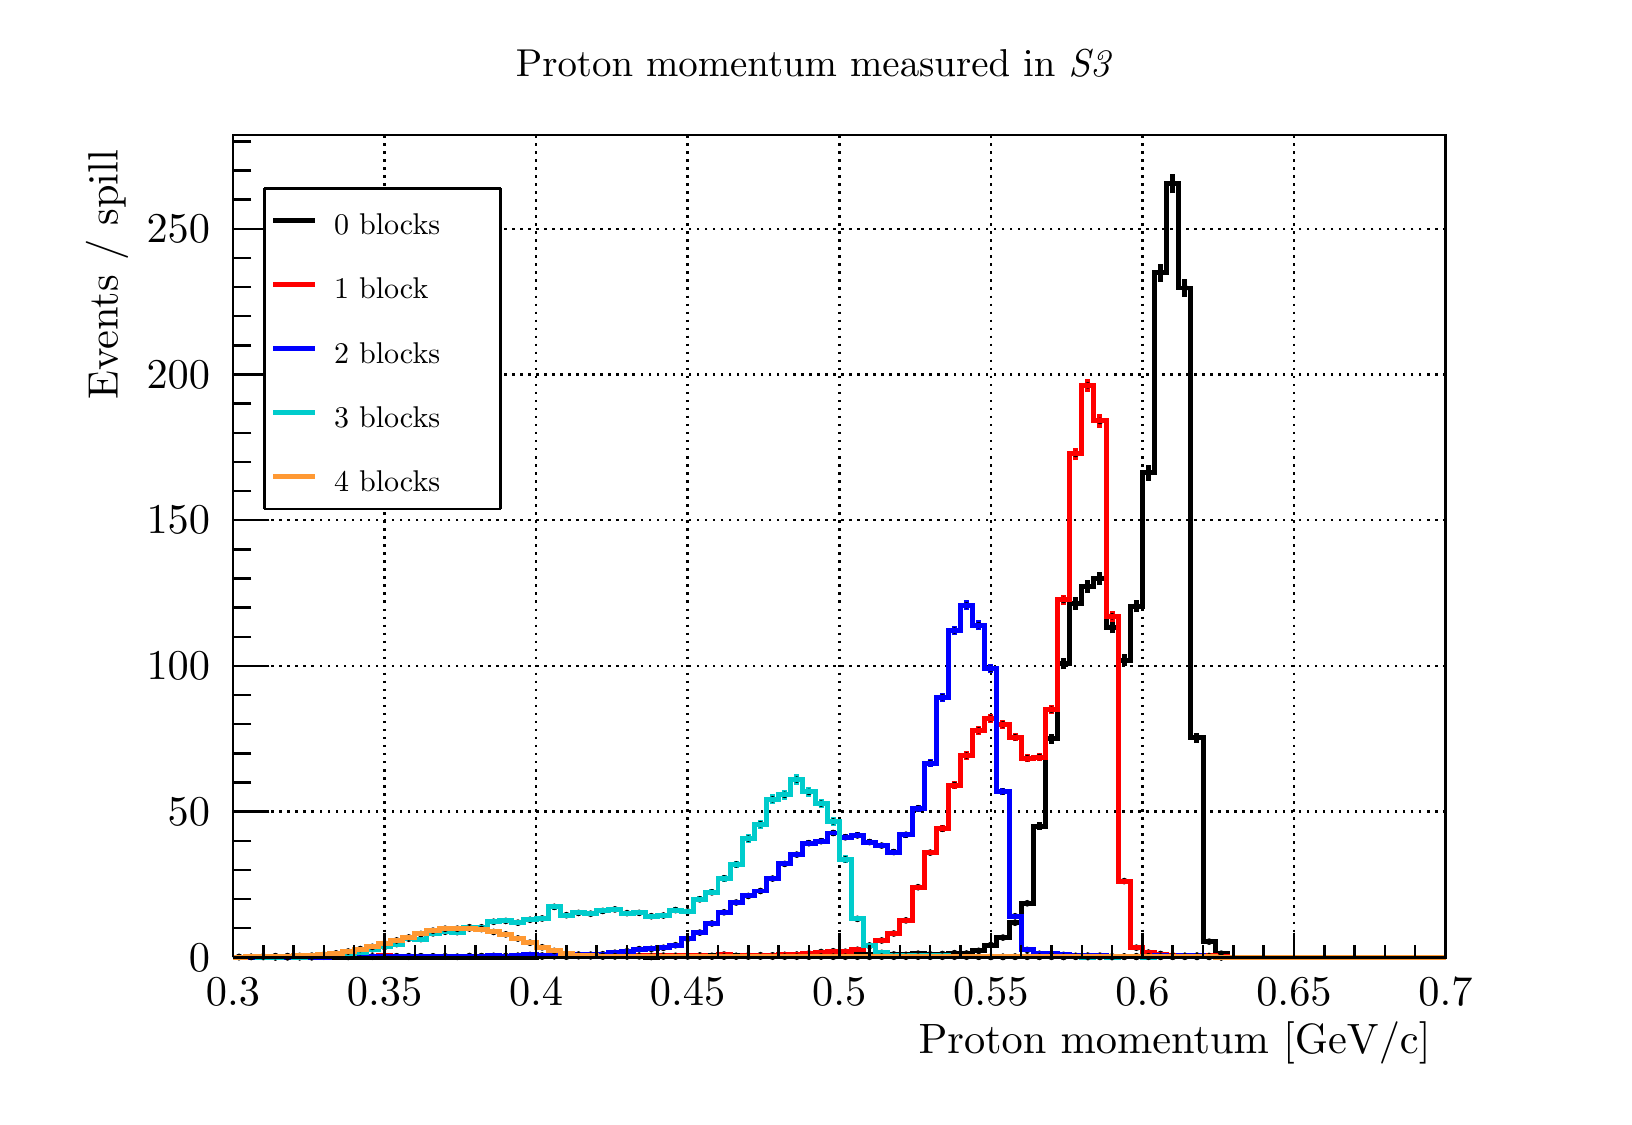
\begin{tikzpicture}
\pgfdeclareplotmark{cross} {
\pgfpathmoveto{\pgfpoint{-0.3\pgfplotmarksize}{\pgfplotmarksize}}
\pgfpathlineto{\pgfpoint{+0.3\pgfplotmarksize}{\pgfplotmarksize}}
\pgfpathlineto{\pgfpoint{+0.3\pgfplotmarksize}{0.3\pgfplotmarksize}}
\pgfpathlineto{\pgfpoint{+1\pgfplotmarksize}{0.3\pgfplotmarksize}}
\pgfpathlineto{\pgfpoint{+1\pgfplotmarksize}{-0.3\pgfplotmarksize}}
\pgfpathlineto{\pgfpoint{+0.3\pgfplotmarksize}{-0.3\pgfplotmarksize}}
\pgfpathlineto{\pgfpoint{+0.3\pgfplotmarksize}{-1.\pgfplotmarksize}}
\pgfpathlineto{\pgfpoint{-0.3\pgfplotmarksize}{-1.\pgfplotmarksize}}
\pgfpathlineto{\pgfpoint{-0.3\pgfplotmarksize}{-0.3\pgfplotmarksize}}
\pgfpathlineto{\pgfpoint{-1.\pgfplotmarksize}{-0.3\pgfplotmarksize}}
\pgfpathlineto{\pgfpoint{-1.\pgfplotmarksize}{0.3\pgfplotmarksize}}
\pgfpathlineto{\pgfpoint{-0.3\pgfplotmarksize}{0.3\pgfplotmarksize}}
\pgfpathclose
\pgfusepathqstroke
}
\pgfdeclareplotmark{cross*} {
\pgfpathmoveto{\pgfpoint{-0.3\pgfplotmarksize}{\pgfplotmarksize}}
\pgfpathlineto{\pgfpoint{+0.3\pgfplotmarksize}{\pgfplotmarksize}}
\pgfpathlineto{\pgfpoint{+0.3\pgfplotmarksize}{0.3\pgfplotmarksize}}
\pgfpathlineto{\pgfpoint{+1\pgfplotmarksize}{0.3\pgfplotmarksize}}
\pgfpathlineto{\pgfpoint{+1\pgfplotmarksize}{-0.3\pgfplotmarksize}}
\pgfpathlineto{\pgfpoint{+0.3\pgfplotmarksize}{-0.3\pgfplotmarksize}}
\pgfpathlineto{\pgfpoint{+0.3\pgfplotmarksize}{-1.\pgfplotmarksize}}
\pgfpathlineto{\pgfpoint{-0.3\pgfplotmarksize}{-1.\pgfplotmarksize}}
\pgfpathlineto{\pgfpoint{-0.3\pgfplotmarksize}{-0.3\pgfplotmarksize}}
\pgfpathlineto{\pgfpoint{-1.\pgfplotmarksize}{-0.3\pgfplotmarksize}}
\pgfpathlineto{\pgfpoint{-1.\pgfplotmarksize}{0.3\pgfplotmarksize}}
\pgfpathlineto{\pgfpoint{-0.3\pgfplotmarksize}{0.3\pgfplotmarksize}}
\pgfpathclose
\pgfusepathqfillstroke
}
\pgfdeclareplotmark{newstar} {
\pgfpathmoveto{\pgfqpoint{0pt}{\pgfplotmarksize}}
\pgfpathlineto{\pgfqpointpolar{44}{0.5\pgfplotmarksize}}
\pgfpathlineto{\pgfqpointpolar{18}{\pgfplotmarksize}}
\pgfpathlineto{\pgfqpointpolar{-20}{0.5\pgfplotmarksize}}
\pgfpathlineto{\pgfqpointpolar{-54}{\pgfplotmarksize}}
\pgfpathlineto{\pgfqpointpolar{-90}{0.5\pgfplotmarksize}}
\pgfpathlineto{\pgfqpointpolar{234}{\pgfplotmarksize}}
\pgfpathlineto{\pgfqpointpolar{198}{0.5\pgfplotmarksize}}
\pgfpathlineto{\pgfqpointpolar{162}{\pgfplotmarksize}}
\pgfpathlineto{\pgfqpointpolar{134}{0.5\pgfplotmarksize}}
\pgfpathclose
\pgfusepathqstroke
}
\pgfdeclareplotmark{newstar*} {
\pgfpathmoveto{\pgfqpoint{0pt}{\pgfplotmarksize}}
\pgfpathlineto{\pgfqpointpolar{44}{0.5\pgfplotmarksize}}
\pgfpathlineto{\pgfqpointpolar{18}{\pgfplotmarksize}}
\pgfpathlineto{\pgfqpointpolar{-20}{0.5\pgfplotmarksize}}
\pgfpathlineto{\pgfqpointpolar{-54}{\pgfplotmarksize}}
\pgfpathlineto{\pgfqpointpolar{-90}{0.5\pgfplotmarksize}}
\pgfpathlineto{\pgfqpointpolar{234}{\pgfplotmarksize}}
\pgfpathlineto{\pgfqpointpolar{198}{0.5\pgfplotmarksize}}
\pgfpathlineto{\pgfqpointpolar{162}{\pgfplotmarksize}}
\pgfpathlineto{\pgfqpointpolar{134}{0.5\pgfplotmarksize}}
\pgfpathclose
\pgfusepathqfillstroke
}
\definecolor{c}{rgb}{1,1,1};
\draw [color=c, fill=c] (0,0) rectangle (20,13.5632);
\draw [color=c, fill=c] (2.6,1.76322) rectangle (18,12.2069);
\definecolor{c}{rgb}{0,0,0};
\draw [c,line width=0.9] (2.6,1.76322) -- (2.6,12.2069) -- (18,12.2069) -- (18,1.76322) -- (2.6,1.76322);
\definecolor{c}{rgb}{1,1,1};
\draw [color=c, fill=c] (2.6,1.76322) rectangle (18,12.2069);
\definecolor{c}{rgb}{0,0,0};
\draw [c,line width=0.9] (2.6,1.76322) -- (2.6,12.2069) -- (18,12.2069) -- (18,1.76322) -- (2.6,1.76322);
\draw [c,line width=0.9] (2.6,1.76322) -- (18,1.76322);
\draw [c,dotted,line width=0.9] (2.6,12.2069) -- (2.6,1.76322);
\draw [c,dotted,line width=0.9] (4.525,12.2069) -- (4.525,1.76322);
\draw [c,dotted,line width=0.9] (6.45,12.2069) -- (6.45,1.76322);
\draw [c,dotted,line width=0.9] (8.375,12.2069) -- (8.375,1.76322);
\draw [c,dotted,line width=0.9] (10.3,12.2069) -- (10.3,1.76322);
\draw [c,dotted,line width=0.9] (12.225,12.2069) -- (12.225,1.76322);
\draw [c,dotted,line width=0.9] (14.15,12.2069) -- (14.15,1.76322);
\draw [c,dotted,line width=0.9] (16.075,12.2069) -- (16.075,1.76322);
\draw [c,dotted,line width=0.9] (18,12.2069) -- (18,1.76322);
\draw [c,line width=0.9] (2.6,1.76322) -- (2.6,12.2069);
\draw [c,dotted,line width=0.9] (18,1.76322) -- (2.6,1.76322);
\draw [c,dotted,line width=0.9] (18,3.61382) -- (2.6,3.61382);
\draw [c,dotted,line width=0.9] (18,5.46443) -- (2.6,5.46443);
\draw [c,dotted,line width=0.9] (18,7.31504) -- (2.6,7.31504);
\draw [c,dotted,line width=0.9] (18,9.16564) -- (2.6,9.16564);
\draw [c,dotted,line width=0.9] (18,11.0162) -- (2.6,11.0162);
\draw [c,dotted,line width=0.9] (18,11.0162) -- (2.6,11.0162);
\definecolor{c}{rgb}{0,0,0.6};
\draw [c,line width=0.9] (2.6,1.76322) -- (2.754,1.76322) -- (2.754,1.76322) -- (2.908,1.76322) -- (2.908,1.76322) -- (3.062,1.76322) -- (3.062,1.76322) -- (3.216,1.76322) -- (3.216,1.76322) -- (3.37,1.76322) -- (3.37,1.76322) -- (3.524,1.76322) --
 (3.524,1.76322) -- (3.678,1.76322) -- (3.678,1.76322) -- (3.832,1.76322) -- (3.832,1.76322) -- (3.986,1.76322) -- (3.986,1.76322) -- (4.14,1.76322) -- (4.14,1.76322) -- (4.294,1.76322) -- (4.294,1.76322) -- (4.448,1.76322) -- (4.448,1.76322) --
 (4.602,1.76322) -- (4.602,1.76322) -- (4.756,1.76322) -- (4.756,1.76322) -- (4.91,1.76322) -- (4.91,1.76322) -- (5.064,1.76322) -- (5.064,1.76322) -- (5.218,1.76322) -- (5.218,1.76322) -- (5.372,1.76322) -- (5.372,1.76322) -- (5.526,1.76322) --
 (5.526,1.76322) -- (5.68,1.76322) -- (5.68,1.76322) -- (5.834,1.76322) -- (5.834,1.76322) -- (5.988,1.76322) -- (5.988,1.76322) -- (6.142,1.76322) -- (6.142,1.76322) -- (6.296,1.76322) -- (6.296,1.76322) -- (6.45,1.76322) -- (6.45,1.76322) --
 (6.604,1.76322) -- (6.604,1.76322) -- (6.758,1.76322) -- (6.758,1.76322) -- (6.912,1.76322) -- (6.912,1.76322) -- (7.066,1.76322) -- (7.066,1.76322) -- (7.22,1.76322) -- (7.22,1.76322) -- (7.374,1.76322) -- (7.374,1.76322) -- (7.528,1.76322) --
 (7.528,1.76322) -- (7.682,1.76322) -- (7.682,1.76322) -- (7.836,1.76322) -- (7.836,1.76322) -- (7.99,1.76322) -- (7.99,1.76322) -- (8.144,1.76322) -- (8.144,1.76322) -- (8.298,1.76322) -- (8.298,1.76322) -- (8.452,1.76322) -- (8.452,1.76322) --
 (8.606,1.76322) -- (8.606,1.76322) -- (8.76,1.76322) -- (8.76,1.76322) -- (8.914,1.76322) -- (8.914,1.76322) -- (9.068,1.76322) -- (9.068,1.76322) -- (9.222,1.76322) -- (9.222,1.76322) -- (9.376,1.76322) -- (9.376,1.76322) -- (9.53,1.76322) --
 (9.53,1.76322) -- (9.684,1.76322) -- (9.684,1.76322) -- (9.838,1.76322) -- (9.838,1.76322) -- (9.992,1.76322) -- (9.992,1.76322) -- (10.146,1.76322) -- (10.146,1.76322) -- (10.3,1.76322) -- (10.3,1.76322) -- (10.454,1.76322) -- (10.454,1.76322) --
 (10.608,1.76322) -- (10.608,1.76322) -- (10.762,1.76322) -- (10.762,1.76322) -- (10.916,1.76322) -- (10.916,1.76322) -- (11.07,1.76322) -- (11.07,1.76322) -- (11.224,1.76322) -- (11.224,1.76322) -- (11.378,1.76322) -- (11.378,1.76322) --
 (11.532,1.76322) -- (11.532,1.76322) -- (11.686,1.76322) -- (11.686,1.76322) -- (11.84,1.76322) -- (11.84,1.76322) -- (11.994,1.76322) -- (11.994,1.76322) -- (12.148,1.76322) -- (12.148,1.76322) -- (12.302,1.76322) -- (12.302,1.76322) --
 (12.456,1.76322) -- (12.456,1.76322) -- (12.61,1.76322) -- (12.61,1.76322) -- (12.764,1.76322) -- (12.764,1.76322) -- (12.918,1.76322) -- (12.918,1.76322) -- (13.072,1.76322) -- (13.072,1.76322) -- (13.226,1.76322) -- (13.226,1.76322) --
 (13.38,1.76322) -- (13.38,1.76322) -- (13.534,1.76322) -- (13.534,1.76322) -- (13.688,1.76322) -- (13.688,1.76322) -- (13.842,1.76322) -- (13.842,1.76322) -- (13.996,1.76322) -- (13.996,1.76322) -- (14.15,1.76322) -- (14.15,1.76322) --
 (14.304,1.76322) -- (14.304,1.76322) -- (14.458,1.76322) -- (14.458,1.76322) -- (14.612,1.76322) -- (14.612,1.76322) -- (14.766,1.76322) -- (14.766,1.76322) -- (14.92,1.76322) -- (14.92,1.76322) -- (15.074,1.76322) -- (15.074,1.76322) --
 (15.228,1.76322) -- (15.228,1.76322) -- (15.382,1.76322) -- (15.382,1.76322) -- (15.536,1.76322) -- (15.536,1.76322) -- (15.69,1.76322) -- (15.69,1.76322) -- (15.844,1.76322) -- (15.844,1.76322) -- (15.998,1.76322) -- (15.998,1.76322) --
 (16.152,1.76322) -- (16.152,1.76322) -- (16.306,1.76322) -- (16.306,1.76322) -- (16.46,1.76322) -- (16.46,1.76322) -- (16.614,1.76322) -- (16.614,1.76322) -- (16.768,1.76322) -- (16.768,1.76322) -- (16.922,1.76322) -- (16.922,1.76322) --
 (17.076,1.76322) -- (17.076,1.76322) -- (17.23,1.76322) -- (17.23,1.76322) -- (17.384,1.76322) -- (17.384,1.76322) -- (17.538,1.76322) -- (17.538,1.76322) -- (17.692,1.76322) -- (17.692,1.76322) -- (17.846,1.76322) -- (17.846,1.76322) --
 (18,1.76322);
\definecolor{c}{rgb}{0,0,0};
\draw [c,line width=0.9] (2.6,1.76322) -- (18,1.76322);
\draw [anchor= east] (18,0.678161) node[scale=1.5317, color=c, rotate=0]{ Proton momentum [GeV/c]};
\draw [c,line width=0.9] (2.6,2.07653) -- (2.6,1.76322);
\draw [c,line width=0.9] (2.985,1.91987) -- (2.985,1.76322);
\draw [c,line width=0.9] (3.37,1.91987) -- (3.37,1.76322);
\draw [c,line width=0.9] (3.755,1.91987) -- (3.755,1.76322);
\draw [c,line width=0.9] (4.14,1.91987) -- (4.14,1.76322);
\draw [c,line width=0.9] (4.525,2.07653) -- (4.525,1.76322);
\draw [c,line width=0.9] (4.91,1.91987) -- (4.91,1.76322);
\draw [c,line width=0.9] (5.295,1.91987) -- (5.295,1.76322);
\draw [c,line width=0.9] (5.68,1.91987) -- (5.68,1.76322);
\draw [c,line width=0.9] (6.065,1.91987) -- (6.065,1.76322);
\draw [c,line width=0.9] (6.45,2.07653) -- (6.45,1.76322);
\draw [c,line width=0.9] (6.835,1.91987) -- (6.835,1.76322);
\draw [c,line width=0.9] (7.22,1.91987) -- (7.22,1.76322);
\draw [c,line width=0.9] (7.605,1.91987) -- (7.605,1.76322);
\draw [c,line width=0.9] (7.99,1.91987) -- (7.99,1.76322);
\draw [c,line width=0.9] (8.375,2.07653) -- (8.375,1.76322);
\draw [c,line width=0.9] (8.76,1.91987) -- (8.76,1.76322);
\draw [c,line width=0.9] (9.145,1.91987) -- (9.145,1.76322);
\draw [c,line width=0.9] (9.53,1.91987) -- (9.53,1.76322);
\draw [c,line width=0.9] (9.915,1.91987) -- (9.915,1.76322);
\draw [c,line width=0.9] (10.3,2.07653) -- (10.3,1.76322);
\draw [c,line width=0.9] (10.685,1.91987) -- (10.685,1.76322);
\draw [c,line width=0.9] (11.07,1.91987) -- (11.07,1.76322);
\draw [c,line width=0.9] (11.455,1.91987) -- (11.455,1.76322);
\draw [c,line width=0.9] (11.84,1.91987) -- (11.84,1.76322);
\draw [c,line width=0.9] (12.225,2.07653) -- (12.225,1.76322);
\draw [c,line width=0.9] (12.61,1.91987) -- (12.61,1.76322);
\draw [c,line width=0.9] (12.995,1.91987) -- (12.995,1.76322);
\draw [c,line width=0.9] (13.38,1.91987) -- (13.38,1.76322);
\draw [c,line width=0.9] (13.765,1.91987) -- (13.765,1.76322);
\draw [c,line width=0.9] (14.15,2.07653) -- (14.15,1.76322);
\draw [c,line width=0.9] (14.535,1.91987) -- (14.535,1.76322);
\draw [c,line width=0.9] (14.92,1.91987) -- (14.92,1.76322);
\draw [c,line width=0.9] (15.305,1.91987) -- (15.305,1.76322);
\draw [c,line width=0.9] (15.69,1.91987) -- (15.69,1.76322);
\draw [c,line width=0.9] (16.075,2.07653) -- (16.075,1.76322);
\draw [c,line width=0.9] (16.46,1.91987) -- (16.46,1.76322);
\draw [c,line width=0.9] (16.845,1.91987) -- (16.845,1.76322);
\draw [c,line width=0.9] (17.23,1.91987) -- (17.23,1.76322);
\draw [c,line width=0.9] (17.615,1.91987) -- (17.615,1.76322);
\draw [c,line width=0.9] (18,2.07653) -- (18,1.76322);
\draw [anchor=base] (2.6,1.15287) node[scale=1.5317, color=c, rotate=0]{0.3};
\draw [anchor=base] (4.525,1.15287) node[scale=1.5317, color=c, rotate=0]{0.35};
\draw [anchor=base] (6.45,1.15287) node[scale=1.5317, color=c, rotate=0]{0.4};
\draw [anchor=base] (8.375,1.15287) node[scale=1.5317, color=c, rotate=0]{0.45};
\draw [anchor=base] (10.3,1.15287) node[scale=1.5317, color=c, rotate=0]{0.5};
\draw [anchor=base] (12.225,1.15287) node[scale=1.5317, color=c, rotate=0]{0.55};
\draw [anchor=base] (14.15,1.15287) node[scale=1.5317, color=c, rotate=0]{0.6};
\draw [anchor=base] (16.075,1.15287) node[scale=1.5317, color=c, rotate=0]{0.65};
\draw [anchor=base] (18,1.15287) node[scale=1.5317, color=c, rotate=0]{0.7};
\draw [c,line width=0.9] (2.6,1.76322) -- (2.6,12.2069);
\draw [anchor= east] (1,12.2069) node[scale=1.5317, color=c, rotate=90]{ Events / spill};
\draw [c,line width=0.9] (3.062,1.76322) -- (2.6,1.76322);
\draw [c,line width=0.9] (2.831,2.13334) -- (2.6,2.13334);
\draw [c,line width=0.9] (2.831,2.50346) -- (2.6,2.50346);
\draw [c,line width=0.9] (2.831,2.87358) -- (2.6,2.87358);
\draw [c,line width=0.9] (2.831,3.2437) -- (2.6,3.2437);
\draw [c,line width=0.9] (3.062,3.61382) -- (2.6,3.61382);
\draw [c,line width=0.9] (2.831,3.98395) -- (2.6,3.98395);
\draw [c,line width=0.9] (2.831,4.35407) -- (2.6,4.35407);
\draw [c,line width=0.9] (2.831,4.72419) -- (2.6,4.72419);
\draw [c,line width=0.9] (2.831,5.09431) -- (2.6,5.09431);
\draw [c,line width=0.9] (3.062,5.46443) -- (2.6,5.46443);
\draw [c,line width=0.9] (2.831,5.83455) -- (2.6,5.83455);
\draw [c,line width=0.9] (2.831,6.20467) -- (2.6,6.20467);
\draw [c,line width=0.9] (2.831,6.57479) -- (2.6,6.57479);
\draw [c,line width=0.9] (2.831,6.94492) -- (2.6,6.94492);
\draw [c,line width=0.9] (3.062,7.31504) -- (2.6,7.31504);
\draw [c,line width=0.9] (2.831,7.68516) -- (2.6,7.68516);
\draw [c,line width=0.9] (2.831,8.05528) -- (2.6,8.05528);
\draw [c,line width=0.9] (2.831,8.4254) -- (2.6,8.4254);
\draw [c,line width=0.9] (2.831,8.79552) -- (2.6,8.79552);
\draw [c,line width=0.9] (3.062,9.16564) -- (2.6,9.16564);
\draw [c,line width=0.9] (2.831,9.53576) -- (2.6,9.53576);
\draw [c,line width=0.9] (2.831,9.90588) -- (2.6,9.90588);
\draw [c,line width=0.9] (2.831,10.276) -- (2.6,10.276);
\draw [c,line width=0.9] (2.831,10.6461) -- (2.6,10.6461);
\draw [c,line width=0.9] (3.062,11.0162) -- (2.6,11.0162);
\draw [c,line width=0.9] (3.062,11.0162) -- (2.6,11.0162);
\draw [c,line width=0.9] (2.831,11.3864) -- (2.6,11.3864);
\draw [c,line width=0.9] (2.831,11.7565) -- (2.6,11.7565);
\draw [c,line width=0.9] (2.831,12.1266) -- (2.6,12.1266);
\draw [anchor= east] (2.5,1.76322) node[scale=1.5317, color=c, rotate=0]{0};
\draw [anchor= east] (2.5,3.61382) node[scale=1.5317, color=c, rotate=0]{50};
\draw [anchor= east] (2.5,5.46443) node[scale=1.5317, color=c, rotate=0]{100};
\draw [anchor= east] (2.5,7.31504) node[scale=1.5317, color=c, rotate=0]{150};
\draw [anchor= east] (2.5,9.16564) node[scale=1.5317, color=c, rotate=0]{200};
\draw [anchor= east] (2.5,11.0162) node[scale=1.5317, color=c, rotate=0]{250};
\draw [c,line width=1.8] (6.527,1.77472) -- (6.527,1.7797);
\draw [c,line width=1.8] (6.527,1.7797) -- (6.527,1.78468);
\foreach \P in {(6.527,1.7797)}{\draw[mark options={color=c,fill=c},mark size=2.402402pt,mark=*,mark size=1pt] plot coordinates {\P};}
\draw [c,line width=1.8] (6.681,1.77299) -- (6.681,1.77753);
\draw [c,line width=1.8] (6.681,1.77753) -- (6.681,1.78208);
\foreach \P in {(6.681,1.77753)}{\draw[mark options={color=c,fill=c},mark size=2.402402pt,mark=*,mark size=1pt] plot coordinates {\P};}
\draw [c,line width=1.8] (6.835,1.77407) -- (6.835,1.77876);
\draw [c,line width=1.8] (6.835,1.77876) -- (6.835,1.78346);
\foreach \P in {(6.835,1.77876)}{\draw[mark options={color=c,fill=c},mark size=2.402402pt,mark=*,mark size=1pt] plot coordinates {\P};}
\draw [c,line width=1.8] (6.989,1.77335) -- (6.989,1.77804);
\draw [c,line width=1.8] (6.989,1.77804) -- (6.989,1.78273);
\foreach \P in {(6.989,1.77804)}{\draw[mark options={color=c,fill=c},mark size=2.402402pt,mark=*,mark size=1pt] plot coordinates {\P};}
\draw [c,line width=1.8] (7.143,1.77209) -- (7.143,1.77657);
\draw [c,line width=1.8] (7.143,1.77657) -- (7.143,1.78105);
\foreach \P in {(7.143,1.77657)}{\draw[mark options={color=c,fill=c},mark size=2.402402pt,mark=*,mark size=1pt] plot coordinates {\P};}
\draw [c,line width=1.8] (7.297,1.76943) -- (7.297,1.77321);
\draw [c,line width=1.8] (7.297,1.77321) -- (7.297,1.77699);
\foreach \P in {(7.297,1.77321)}{\draw[mark options={color=c,fill=c},mark size=2.402402pt,mark=*,mark size=1pt] plot coordinates {\P};}
\draw [c,line width=1.8] (7.451,1.77679) -- (7.451,1.78205);
\draw [c,line width=1.8] (7.451,1.78205) -- (7.451,1.78731);
\foreach \P in {(7.451,1.78205)}{\draw[mark options={color=c,fill=c},mark size=2.402402pt,mark=*,mark size=1pt] plot coordinates {\P};}
\draw [c,line width=1.8] (7.605,1.77314) -- (7.605,1.77778);
\draw [c,line width=1.8] (7.605,1.77778) -- (7.605,1.78242);
\foreach \P in {(7.605,1.77778)}{\draw[mark options={color=c,fill=c},mark size=2.402402pt,mark=*,mark size=1pt] plot coordinates {\P};}
\draw [c,line width=1.8] (7.759,1.77644) -- (7.759,1.78153);
\draw [c,line width=1.8] (7.759,1.78153) -- (7.759,1.78663);
\foreach \P in {(7.759,1.78153)}{\draw[mark options={color=c,fill=c},mark size=2.402402pt,mark=*,mark size=1pt] plot coordinates {\P};}
\draw [c,line width=1.8] (7.913,1.76506) -- (7.913,1.76758);
\draw [c,line width=1.8] (7.913,1.76758) -- (7.913,1.77009);
\foreach \P in {(7.913,1.76758)}{\draw[mark options={color=c,fill=c},mark size=2.402402pt,mark=*,mark size=1pt] plot coordinates {\P};}
\draw [c,line width=1.8] (8.067,1.77225) -- (8.067,1.7768);
\draw [c,line width=1.8] (8.067,1.7768) -- (8.067,1.78135);
\foreach \P in {(8.067,1.7768)}{\draw[mark options={color=c,fill=c},mark size=2.402402pt,mark=*,mark size=1pt] plot coordinates {\P};}
\draw [c,line width=1.8] (8.221,1.77071) -- (8.221,1.77485);
\draw [c,line width=1.8] (8.221,1.77485) -- (8.221,1.77899);
\foreach \P in {(8.221,1.77485)}{\draw[mark options={color=c,fill=c},mark size=2.402402pt,mark=*,mark size=1pt] plot coordinates {\P};}
\draw [c,line width=1.8] (8.375,1.77688) -- (8.375,1.78215);
\draw [c,line width=1.8] (8.375,1.78215) -- (8.375,1.78743);
\foreach \P in {(8.375,1.78215)}{\draw[mark options={color=c,fill=c},mark size=2.402402pt,mark=*,mark size=1pt] plot coordinates {\P};}
\draw [c,line width=1.8] (8.529,1.77958) -- (8.529,1.7853);
\draw [c,line width=1.8] (8.529,1.7853) -- (8.529,1.79101);
\foreach \P in {(8.529,1.7853)}{\draw[mark options={color=c,fill=c},mark size=2.402402pt,mark=*,mark size=1pt] plot coordinates {\P};}
\draw [c,line width=1.8] (8.683,1.77734) -- (8.683,1.78279);
\draw [c,line width=1.8] (8.683,1.78279) -- (8.683,1.78824);
\foreach \P in {(8.683,1.78279)}{\draw[mark options={color=c,fill=c},mark size=2.402402pt,mark=*,mark size=1pt] plot coordinates {\P};}
\draw [c,line width=1.8] (8.837,1.77226) -- (8.837,1.77681);
\draw [c,line width=1.8] (8.837,1.77681) -- (8.837,1.78137);
\foreach \P in {(8.837,1.77681)}{\draw[mark options={color=c,fill=c},mark size=2.402402pt,mark=*,mark size=1pt] plot coordinates {\P};}
\draw [c,line width=1.8] (8.991,1.77726) -- (8.991,1.78269);
\draw [c,line width=1.8] (8.991,1.78269) -- (8.991,1.78812);
\foreach \P in {(8.991,1.78269)}{\draw[mark options={color=c,fill=c},mark size=2.402402pt,mark=*,mark size=1pt] plot coordinates {\P};}
\draw [c,line width=1.8] (9.145,1.78107) -- (9.145,1.78706);
\draw [c,line width=1.8] (9.145,1.78706) -- (9.145,1.79305);
\foreach \P in {(9.145,1.78706)}{\draw[mark options={color=c,fill=c},mark size=2.402402pt,mark=*,mark size=1pt] plot coordinates {\P};}
\draw [c,line width=1.8] (9.299,1.77668) -- (9.299,1.78186);
\draw [c,line width=1.8] (9.299,1.78186) -- (9.299,1.78704);
\foreach \P in {(9.299,1.78186)}{\draw[mark options={color=c,fill=c},mark size=2.402402pt,mark=*,mark size=1pt] plot coordinates {\P};}
\draw [c,line width=1.8] (9.453,1.77923) -- (9.453,1.78483);
\draw [c,line width=1.8] (9.453,1.78483) -- (9.453,1.79044);
\foreach \P in {(9.453,1.78483)}{\draw[mark options={color=c,fill=c},mark size=2.402402pt,mark=*,mark size=1pt] plot coordinates {\P};}
\draw [c,line width=1.8] (9.607,1.78653) -- (9.607,1.79328);
\draw [c,line width=1.8] (9.607,1.79328) -- (9.607,1.80003);
\foreach \P in {(9.607,1.79328)}{\draw[mark options={color=c,fill=c},mark size=2.402402pt,mark=*,mark size=1pt] plot coordinates {\P};}
\draw [c,line width=1.8] (9.761,1.78853) -- (9.761,1.79545);
\draw [c,line width=1.8] (9.761,1.79545) -- (9.761,1.80237);
\foreach \P in {(9.761,1.79545)}{\draw[mark options={color=c,fill=c},mark size=2.402402pt,mark=*,mark size=1pt] plot coordinates {\P};}
\draw [c,line width=1.8] (9.915,1.77682) -- (9.915,1.78206);
\draw [c,line width=1.8] (9.915,1.78206) -- (9.915,1.7873);
\foreach \P in {(9.915,1.78206)}{\draw[mark options={color=c,fill=c},mark size=2.402402pt,mark=*,mark size=1pt] plot coordinates {\P};}
\draw [c,line width=1.8] (10.069,1.78289) -- (10.069,1.78902);
\draw [c,line width=1.8] (10.069,1.78902) -- (10.069,1.79514);
\foreach \P in {(10.069,1.78902)}{\draw[mark options={color=c,fill=c},mark size=2.402402pt,mark=*,mark size=1pt] plot coordinates {\P};}
\draw [c,line width=1.8] (10.223,1.77295) -- (10.223,1.77748);
\draw [c,line width=1.8] (10.223,1.77748) -- (10.223,1.782);
\foreach \P in {(10.223,1.77748)}{\draw[mark options={color=c,fill=c},mark size=2.402402pt,mark=*,mark size=1pt] plot coordinates {\P};}
\draw [c,line width=1.8] (10.377,1.78119) -- (10.377,1.78724);
\draw [c,line width=1.8] (10.377,1.78724) -- (10.377,1.79328);
\foreach \P in {(10.377,1.78724)}{\draw[mark options={color=c,fill=c},mark size=2.402402pt,mark=*,mark size=1pt] plot coordinates {\P};}
\draw [c,line width=1.8] (10.531,1.78773) -- (10.531,1.79462);
\draw [c,line width=1.8] (10.531,1.79462) -- (10.531,1.8015);
\foreach \P in {(10.531,1.79462)}{\draw[mark options={color=c,fill=c},mark size=2.402402pt,mark=*,mark size=1pt] plot coordinates {\P};}
\draw [c,line width=1.8] (10.685,1.78806) -- (10.685,1.79482);
\draw [c,line width=1.8] (10.685,1.79482) -- (10.685,1.80158);
\foreach \P in {(10.685,1.79482)}{\draw[mark options={color=c,fill=c},mark size=2.402402pt,mark=*,mark size=1pt] plot coordinates {\P};}
\draw [c,line width=1.8] (10.839,1.79316) -- (10.839,1.80072);
\draw [c,line width=1.8] (10.839,1.80072) -- (10.839,1.80828);
\foreach \P in {(10.839,1.80072)}{\draw[mark options={color=c,fill=c},mark size=2.402402pt,mark=*,mark size=1pt] plot coordinates {\P};}
\draw [c,line width=1.8] (10.993,1.79236) -- (10.993,1.79968);
\draw [c,line width=1.8] (10.993,1.79968) -- (10.993,1.807);
\foreach \P in {(10.993,1.79968)}{\draw[mark options={color=c,fill=c},mark size=2.402402pt,mark=*,mark size=1pt] plot coordinates {\P};}
\draw [c,line width=1.8] (11.147,1.78826) -- (11.147,1.79529);
\draw [c,line width=1.8] (11.147,1.79529) -- (11.147,1.80232);
\foreach \P in {(11.147,1.79529)}{\draw[mark options={color=c,fill=c},mark size=2.402402pt,mark=*,mark size=1pt] plot coordinates {\P};}
\draw [c,line width=1.8] (11.301,1.80144) -- (11.301,1.80988);
\draw [c,line width=1.8] (11.301,1.80988) -- (11.301,1.81831);
\foreach \P in {(11.301,1.80988)}{\draw[mark options={color=c,fill=c},mark size=2.402402pt,mark=*,mark size=1pt] plot coordinates {\P};}
\draw [c,line width=1.8] (11.455,1.79317) -- (11.455,1.80051);
\draw [c,line width=1.8] (11.455,1.80051) -- (11.455,1.80784);
\foreach \P in {(11.455,1.80051)}{\draw[mark options={color=c,fill=c},mark size=2.402402pt,mark=*,mark size=1pt] plot coordinates {\P};}
\draw [c,line width=1.8] (11.609,1.79739) -- (11.609,1.80541);
\draw [c,line width=1.8] (11.609,1.80541) -- (11.609,1.81343);
\foreach \P in {(11.609,1.80541)}{\draw[mark options={color=c,fill=c},mark size=2.402402pt,mark=*,mark size=1pt] plot coordinates {\P};}
\draw [c,line width=1.8] (11.763,1.8075) -- (11.763,1.81626);
\draw [c,line width=1.8] (11.763,1.81626) -- (11.763,1.82503);
\foreach \P in {(11.763,1.81626)}{\draw[mark options={color=c,fill=c},mark size=2.402402pt,mark=*,mark size=1pt] plot coordinates {\P};}
\draw [c,line width=1.8] (11.917,1.80354) -- (11.917,1.81225);
\draw [c,line width=1.8] (11.917,1.81225) -- (11.917,1.82097);
\foreach \P in {(11.917,1.81225)}{\draw[mark options={color=c,fill=c},mark size=2.402402pt,mark=*,mark size=1pt] plot coordinates {\P};}
\draw [c,line width=1.8] (12.071,1.83556) -- (12.071,1.84657);
\draw [c,line width=1.8] (12.071,1.84657) -- (12.071,1.85758);
\foreach \P in {(12.071,1.84657)}{\draw[mark options={color=c,fill=c},mark size=2.402402pt,mark=*,mark size=1pt] plot coordinates {\P};}
\draw [c,line width=1.8] (12.225,1.90447) -- (12.225,1.91974);
\draw [c,line width=1.8] (12.225,1.91974) -- (12.225,1.93502);
\foreach \P in {(12.225,1.91974)}{\draw[mark options={color=c,fill=c},mark size=2.402402pt,mark=*,mark size=1pt] plot coordinates {\P};}
\draw [c,line width=1.8] (12.379,1.99489) -- (12.379,2.01426);
\draw [c,line width=1.8] (12.379,2.01426) -- (12.379,2.03364);
\foreach \P in {(12.379,2.01426)}{\draw[mark options={color=c,fill=c},mark size=2.402402pt,mark=*,mark size=1pt] plot coordinates {\P};}
\draw [c,line width=1.8] (12.533,2.17709) -- (12.533,2.20271);
\draw [c,line width=1.8] (12.533,2.20271) -- (12.533,2.22833);
\foreach \P in {(12.533,2.20271)}{\draw[mark options={color=c,fill=c},mark size=2.402402pt,mark=*,mark size=1pt] plot coordinates {\P};}
\draw [c,line width=1.8] (12.687,2.41778) -- (12.687,2.44984);
\draw [c,line width=1.8] (12.687,2.44984) -- (12.687,2.4819);
\foreach \P in {(12.687,2.44984)}{\draw[mark options={color=c,fill=c},mark size=2.402402pt,mark=*,mark size=1pt] plot coordinates {\P};}
\draw [c,line width=1.8] (12.841,3.37881) -- (12.841,3.42872);
\draw [c,line width=1.8] (12.841,3.42872) -- (12.841,3.47864);
\foreach \P in {(12.841,3.42872)}{\draw[mark options={color=c,fill=c},mark size=2.402402pt,mark=*,mark size=1pt] plot coordinates {\P};}
\draw [c,line width=1.8] (12.995,4.4751) -- (12.995,4.53956);
\draw [c,line width=1.8] (12.995,4.53956) -- (12.995,4.60402);
\foreach \P in {(12.995,4.53956)}{\draw[mark options={color=c,fill=c},mark size=2.402402pt,mark=*,mark size=1pt] plot coordinates {\P};}
\draw [c,line width=1.8] (13.149,5.41981) -- (13.149,5.49452);
\draw [c,line width=1.8] (13.149,5.49452) -- (13.149,5.56924);
\foreach \P in {(13.149,5.49452)}{\draw[mark options={color=c,fill=c},mark size=2.402402pt,mark=*,mark size=1pt] plot coordinates {\P};}
\draw [c,line width=1.8] (13.303,6.17215) -- (13.303,6.25403);
\draw [c,line width=1.8] (13.303,6.25403) -- (13.303,6.33591);
\foreach \P in {(13.303,6.25403)}{\draw[mark options={color=c,fill=c},mark size=2.402402pt,mark=*,mark size=1pt] plot coordinates {\P};}
\draw [c,line width=1.8] (13.457,6.38848) -- (13.457,6.47218);
\draw [c,line width=1.8] (13.457,6.47218) -- (13.457,6.55589);
\foreach \P in {(13.457,6.47218)}{\draw[mark options={color=c,fill=c},mark size=2.402402pt,mark=*,mark size=1pt] plot coordinates {\P};}
\draw [c,line width=1.8] (13.611,6.49068) -- (13.611,6.57534);
\draw [c,line width=1.8] (13.611,6.57534) -- (13.611,6.65999);
\foreach \P in {(13.611,6.57534)}{\draw[mark options={color=c,fill=c},mark size=2.402402pt,mark=*,mark size=1pt] plot coordinates {\P};}
\draw [c,line width=1.8] (13.765,5.8785) -- (13.765,5.95754);
\draw [c,line width=1.8] (13.765,5.95754) -- (13.765,6.03658);
\foreach \P in {(13.765,5.95754)}{\draw[mark options={color=c,fill=c},mark size=2.402402pt,mark=*,mark size=1pt] plot coordinates {\P};}
\draw [c,line width=1.8] (13.919,5.46117) -- (13.919,5.53633);
\draw [c,line width=1.8] (13.919,5.53633) -- (13.919,5.61149);
\foreach \P in {(13.919,5.53633)}{\draw[mark options={color=c,fill=c},mark size=2.402402pt,mark=*,mark size=1pt] plot coordinates {\P};}
\draw [c,line width=1.8] (14.073,6.14327) -- (14.073,6.2249);
\draw [c,line width=1.8] (14.073,6.2249) -- (14.073,6.30653);
\foreach \P in {(14.073,6.2249)}{\draw[mark options={color=c,fill=c},mark size=2.402402pt,mark=*,mark size=1pt] plot coordinates {\P};}
\draw [c,line width=1.8] (14.227,7.81881) -- (14.227,7.91463);
\draw [c,line width=1.8] (14.227,7.91463) -- (14.227,8.01046);
\foreach \P in {(14.227,7.91463)}{\draw[mark options={color=c,fill=c},mark size=2.402402pt,mark=*,mark size=1pt] plot coordinates {\P};}
\draw [c,line width=1.8] (14.381,10.3441) -- (14.381,10.4582);
\draw [c,line width=1.8] (14.381,10.4582) -- (14.381,10.5724);
\foreach \P in {(14.381,10.4582)}{\draw[mark options={color=c,fill=c},mark size=2.402402pt,mark=*,mark size=1pt] plot coordinates {\P};}
\draw [c,line width=1.8] (14.535,11.4672) -- (14.535,11.5884);
\draw [c,line width=1.8] (14.535,11.5884) -- (14.535,11.7096);
\foreach \P in {(14.535,11.5884)}{\draw[mark options={color=c,fill=c},mark size=2.402402pt,mark=*,mark size=1pt] plot coordinates {\P};}
\draw [c,line width=1.8] (14.689,10.1512) -- (14.689,10.264);
\draw [c,line width=1.8] (14.689,10.264) -- (14.689,10.3768);
\foreach \P in {(14.689,10.264)}{\draw[mark options={color=c,fill=c},mark size=2.402402pt,mark=*,mark size=1pt] plot coordinates {\P};}
\draw [c,line width=1.8] (14.843,4.48823) -- (14.843,4.55278);
\draw [c,line width=1.8] (14.843,4.55278) -- (14.843,4.61733);
\foreach \P in {(14.843,4.55278)}{\draw[mark options={color=c,fill=c},mark size=2.402402pt,mark=*,mark size=1pt] plot coordinates {\P};}
\draw [c,line width=1.8] (14.997,1.94581) -- (14.997,1.96298);
\draw [c,line width=1.8] (14.997,1.96298) -- (14.997,1.98015);
\foreach \P in {(14.997,1.96298)}{\draw[mark options={color=c,fill=c},mark size=2.402402pt,mark=*,mark size=1pt] plot coordinates {\P};}
\draw [c,line width=1.8] (15.151,1.80171) -- (15.151,1.81003);
\draw [c,line width=1.8] (15.151,1.81003) -- (15.151,1.81834);
\foreach \P in {(15.151,1.81003)}{\draw[mark options={color=c,fill=c},mark size=2.402402pt,mark=*,mark size=1pt] plot coordinates {\P};}
\draw [c,line width=1.8] (2.6,1.76322) -- (2.754,1.76322) -- (2.754,1.76322) -- (2.908,1.76322) -- (2.908,1.76322) -- (3.062,1.76322) -- (3.062,1.76322) -- (3.216,1.76322) -- (3.216,1.76322) -- (3.37,1.76322) -- (3.37,1.76322) -- (3.524,1.76322) --
 (3.524,1.76322) -- (3.678,1.76322) -- (3.678,1.76322) -- (3.832,1.76322) -- (3.832,1.76322) -- (3.986,1.76322) -- (3.986,1.76322) -- (4.14,1.76322) -- (4.14,1.76322) -- (4.294,1.76322) -- (4.294,1.76322) -- (4.448,1.76322) -- (4.448,1.76322) --
 (4.602,1.76322) -- (4.602,1.76322) -- (4.756,1.76322) -- (4.756,1.76322) -- (4.91,1.76322) -- (4.91,1.76322) -- (5.064,1.76322) -- (5.064,1.76322) -- (5.218,1.76322) -- (5.218,1.76322) -- (5.372,1.76322) -- (5.372,1.76322) -- (5.526,1.76322) --
 (5.526,1.76322) -- (5.68,1.76322) -- (5.68,1.76322) -- (5.834,1.76322) -- (5.834,1.76322) -- (5.988,1.76322) -- (5.988,1.76322) -- (6.142,1.76322) -- (6.142,1.76322) -- (6.296,1.76322) -- (6.296,1.76322) -- (6.45,1.76322) -- (6.45,1.7797) --
 (6.604,1.7797) -- (6.604,1.77753) -- (6.758,1.77753) -- (6.758,1.77876) -- (6.912,1.77876) -- (6.912,1.77804) -- (7.066,1.77804) -- (7.066,1.77657) -- (7.22,1.77657) -- (7.22,1.77321) -- (7.374,1.77321) -- (7.374,1.78205) -- (7.528,1.78205) --
 (7.528,1.77778) -- (7.682,1.77778) -- (7.682,1.78153) -- (7.836,1.78153) -- (7.836,1.76758) -- (7.99,1.76758) -- (7.99,1.7768) -- (8.144,1.7768) -- (8.144,1.77485) -- (8.298,1.77485) -- (8.298,1.78215) -- (8.452,1.78215) -- (8.452,1.7853) --
 (8.606,1.7853) -- (8.606,1.78279) -- (8.76,1.78279) -- (8.76,1.77681) -- (8.914,1.77681) -- (8.914,1.78269) -- (9.068,1.78269) -- (9.068,1.78706) -- (9.222,1.78706) -- (9.222,1.78186) -- (9.376,1.78186) -- (9.376,1.78483) -- (9.53,1.78483) --
 (9.53,1.79328) -- (9.684,1.79328) -- (9.684,1.79545) -- (9.838,1.79545) -- (9.838,1.78206) -- (9.992,1.78206) -- (9.992,1.78902) -- (10.146,1.78902) -- (10.146,1.77748) -- (10.3,1.77748) -- (10.3,1.78724) -- (10.454,1.78724) -- (10.454,1.79462) --
 (10.608,1.79462) -- (10.608,1.79482) -- (10.762,1.79482) -- (10.762,1.80072) -- (10.916,1.80072) -- (10.916,1.79968) -- (11.07,1.79968) -- (11.07,1.79529) -- (11.224,1.79529) -- (11.224,1.80988) -- (11.378,1.80988) -- (11.378,1.80051) --
 (11.532,1.80051) -- (11.532,1.80541) -- (11.686,1.80541) -- (11.686,1.81626) -- (11.84,1.81626) -- (11.84,1.81225) -- (11.994,1.81225) -- (11.994,1.84657) -- (12.148,1.84657) -- (12.148,1.91974) -- (12.302,1.91974) -- (12.302,2.01426) --
 (12.456,2.01426) -- (12.456,2.20271) -- (12.61,2.20271) -- (12.61,2.44984) -- (12.764,2.44984) -- (12.764,3.42872) -- (12.918,3.42872) -- (12.918,4.53956) -- (13.072,4.53956) -- (13.072,5.49452) -- (13.226,5.49452) -- (13.226,6.25403) --
 (13.38,6.25403) -- (13.38,6.47218) -- (13.534,6.47218) -- (13.534,6.57534) -- (13.688,6.57534) -- (13.688,5.95754) -- (13.842,5.95754) -- (13.842,5.53633) -- (13.996,5.53633) -- (13.996,6.2249) -- (14.15,6.2249) -- (14.15,7.91463) --
 (14.304,7.91463) -- (14.304,10.4582) -- (14.458,10.4582) -- (14.458,11.5884) -- (14.612,11.5884) -- (14.612,10.264) -- (14.766,10.264) -- (14.766,4.55278) -- (14.92,4.55278) -- (14.92,1.96298) -- (15.074,1.96298) -- (15.074,1.81003) --
 (15.228,1.81003) -- (15.228,1.76322) -- (15.382,1.76322) -- (15.382,1.76322) -- (15.536,1.76322) -- (15.536,1.76322) -- (15.69,1.76322) -- (15.69,1.76322) -- (15.844,1.76322) -- (15.844,1.76322) -- (15.998,1.76322) -- (15.998,1.76322) --
 (16.152,1.76322) -- (16.152,1.76322) -- (16.306,1.76322) -- (16.306,1.76322) -- (16.46,1.76322) -- (16.46,1.76322) -- (16.614,1.76322) -- (16.614,1.76322) -- (16.768,1.76322) -- (16.768,1.76322) -- (16.922,1.76322) -- (16.922,1.76322) --
 (17.076,1.76322) -- (17.076,1.76322) -- (17.23,1.76322) -- (17.23,1.76322) -- (17.384,1.76322) -- (17.384,1.76322) -- (17.538,1.76322) -- (17.538,1.76322) -- (17.692,1.76322) -- (17.692,1.76322) -- (17.846,1.76322) -- (17.846,1.76322) --
 (18,1.76322);
\definecolor{c}{rgb}{1,0,0};
\draw [c,line width=1.8] (3.139,1.76322) -- (3.139,1.76437);
\draw [c,line width=1.8] (3.139,1.76437) -- (3.139,1.76552);
\definecolor{c}{rgb}{0,0,0};
\foreach \P in {(3.139,1.76437)}{\draw[mark options={color=c,fill=c},mark size=2.402402pt,mark=*,mark size=1pt] plot coordinates {\P};}
\definecolor{c}{rgb}{1,0,0};
\draw [c,line width=1.8] (3.293,1.7645) -- (3.293,1.76626);
\draw [c,line width=1.8] (3.293,1.76626) -- (3.293,1.76802);
\definecolor{c}{rgb}{0,0,0};
\foreach \P in {(3.293,1.76626)}{\draw[mark options={color=c,fill=c},mark size=2.402402pt,mark=*,mark size=1pt] plot coordinates {\P};}
\definecolor{c}{rgb}{1,0,0};
\draw [c,line width=1.8] (3.447,1.76504) -- (3.447,1.76688);
\draw [c,line width=1.8] (3.447,1.76688) -- (3.447,1.76871);
\definecolor{c}{rgb}{0,0,0};
\foreach \P in {(3.447,1.76688)}{\draw[mark options={color=c,fill=c},mark size=2.402402pt,mark=*,mark size=1pt] plot coordinates {\P};}
\definecolor{c}{rgb}{1,0,0};
\draw [c,line width=1.8] (3.601,1.765) -- (3.601,1.76682);
\draw [c,line width=1.8] (3.601,1.76682) -- (3.601,1.76864);
\definecolor{c}{rgb}{0,0,0};
\foreach \P in {(3.601,1.76682)}{\draw[mark options={color=c,fill=c},mark size=2.402402pt,mark=*,mark size=1pt] plot coordinates {\P};}
\definecolor{c}{rgb}{1,0,0};
\draw [c,line width=1.8] (3.755,1.76792) -- (3.755,1.77093);
\draw [c,line width=1.8] (3.755,1.77093) -- (3.755,1.77394);
\definecolor{c}{rgb}{0,0,0};
\foreach \P in {(3.755,1.77093)}{\draw[mark options={color=c,fill=c},mark size=2.402402pt,mark=*,mark size=1pt] plot coordinates {\P};}
\definecolor{c}{rgb}{1,0,0};
\draw [c,line width=1.8] (3.909,1.76974) -- (3.909,1.77308);
\draw [c,line width=1.8] (3.909,1.77308) -- (3.909,1.77643);
\definecolor{c}{rgb}{0,0,0};
\foreach \P in {(3.909,1.77308)}{\draw[mark options={color=c,fill=c},mark size=2.402402pt,mark=*,mark size=1pt] plot coordinates {\P};}
\definecolor{c}{rgb}{1,0,0};
\draw [c,line width=1.8] (4.063,1.76876) -- (4.063,1.77182);
\draw [c,line width=1.8] (4.063,1.77182) -- (4.063,1.77488);
\definecolor{c}{rgb}{0,0,0};
\foreach \P in {(4.063,1.77182)}{\draw[mark options={color=c,fill=c},mark size=2.402402pt,mark=*,mark size=1pt] plot coordinates {\P};}
\definecolor{c}{rgb}{1,0,0};
\draw [c,line width=1.8] (4.217,1.76941) -- (4.217,1.7726);
\draw [c,line width=1.8] (4.217,1.7726) -- (4.217,1.77578);
\definecolor{c}{rgb}{0,0,0};
\foreach \P in {(4.217,1.7726)}{\draw[mark options={color=c,fill=c},mark size=2.402402pt,mark=*,mark size=1pt] plot coordinates {\P};}
\definecolor{c}{rgb}{1,0,0};
\draw [c,line width=1.8] (4.371,1.76852) -- (4.371,1.77148);
\draw [c,line width=1.8] (4.371,1.77148) -- (4.371,1.77443);
\definecolor{c}{rgb}{0,0,0};
\foreach \P in {(4.371,1.77148)}{\draw[mark options={color=c,fill=c},mark size=2.402402pt,mark=*,mark size=1pt] plot coordinates {\P};}
\definecolor{c}{rgb}{1,0,0};
\draw [c,line width=1.8] (4.525,1.77764) -- (4.525,1.78201);
\draw [c,line width=1.8] (4.525,1.78201) -- (4.525,1.78639);
\definecolor{c}{rgb}{0,0,0};
\foreach \P in {(4.525,1.78201)}{\draw[mark options={color=c,fill=c},mark size=2.402402pt,mark=*,mark size=1pt] plot coordinates {\P};}
\definecolor{c}{rgb}{1,0,0};
\draw [c,line width=1.8] (4.679,1.77281) -- (4.679,1.77657);
\draw [c,line width=1.8] (4.679,1.77657) -- (4.679,1.78033);
\definecolor{c}{rgb}{0,0,0};
\foreach \P in {(4.679,1.77657)}{\draw[mark options={color=c,fill=c},mark size=2.402402pt,mark=*,mark size=1pt] plot coordinates {\P};}
\definecolor{c}{rgb}{1,0,0};
\draw [c,line width=1.8] (4.833,1.77444) -- (4.833,1.77838);
\draw [c,line width=1.8] (4.833,1.77838) -- (4.833,1.78233);
\definecolor{c}{rgb}{0,0,0};
\foreach \P in {(4.833,1.77838)}{\draw[mark options={color=c,fill=c},mark size=2.402402pt,mark=*,mark size=1pt] plot coordinates {\P};}
\definecolor{c}{rgb}{1,0,0};
\draw [c,line width=1.8] (4.987,1.77131) -- (4.987,1.77463);
\draw [c,line width=1.8] (4.987,1.77463) -- (4.987,1.77794);
\definecolor{c}{rgb}{0,0,0};
\foreach \P in {(4.987,1.77463)}{\draw[mark options={color=c,fill=c},mark size=2.402402pt,mark=*,mark size=1pt] plot coordinates {\P};}
\definecolor{c}{rgb}{1,0,0};
\draw [c,line width=1.8] (5.141,1.77002) -- (5.141,1.77322);
\draw [c,line width=1.8] (5.141,1.77322) -- (5.141,1.77643);
\definecolor{c}{rgb}{0,0,0};
\foreach \P in {(5.141,1.77322)}{\draw[mark options={color=c,fill=c},mark size=2.402402pt,mark=*,mark size=1pt] plot coordinates {\P};}
\definecolor{c}{rgb}{1,0,0};
\draw [c,line width=1.8] (5.295,1.7691) -- (5.295,1.77219);
\draw [c,line width=1.8] (5.295,1.77219) -- (5.295,1.77528);
\definecolor{c}{rgb}{0,0,0};
\foreach \P in {(5.295,1.77219)}{\draw[mark options={color=c,fill=c},mark size=2.402402pt,mark=*,mark size=1pt] plot coordinates {\P};}
\definecolor{c}{rgb}{1,0,0};
\draw [c,line width=1.8] (5.449,1.76756) -- (5.449,1.77026);
\draw [c,line width=1.8] (5.449,1.77026) -- (5.449,1.77296);
\definecolor{c}{rgb}{0,0,0};
\foreach \P in {(5.449,1.77026)}{\draw[mark options={color=c,fill=c},mark size=2.402402pt,mark=*,mark size=1pt] plot coordinates {\P};}
\definecolor{c}{rgb}{1,0,0};
\draw [c,line width=1.8] (5.603,1.76917) -- (5.603,1.77223);
\draw [c,line width=1.8] (5.603,1.77223) -- (5.603,1.77529);
\definecolor{c}{rgb}{0,0,0};
\foreach \P in {(5.603,1.77223)}{\draw[mark options={color=c,fill=c},mark size=2.402402pt,mark=*,mark size=1pt] plot coordinates {\P};}
\definecolor{c}{rgb}{1,0,0};
\draw [c,line width=1.8] (5.757,1.77233) -- (5.757,1.77607);
\draw [c,line width=1.8] (5.757,1.77607) -- (5.757,1.7798);
\definecolor{c}{rgb}{0,0,0};
\foreach \P in {(5.757,1.77607)}{\draw[mark options={color=c,fill=c},mark size=2.402402pt,mark=*,mark size=1pt] plot coordinates {\P};}
\definecolor{c}{rgb}{1,0,0};
\draw [c,line width=1.8] (5.911,1.77224) -- (5.911,1.77555);
\draw [c,line width=1.8] (5.911,1.77555) -- (5.911,1.77886);
\definecolor{c}{rgb}{0,0,0};
\foreach \P in {(5.911,1.77555)}{\draw[mark options={color=c,fill=c},mark size=2.402402pt,mark=*,mark size=1pt] plot coordinates {\P};}
\definecolor{c}{rgb}{1,0,0};
\draw [c,line width=1.8] (6.065,1.77082) -- (6.065,1.77419);
\draw [c,line width=1.8] (6.065,1.77419) -- (6.065,1.77756);
\definecolor{c}{rgb}{0,0,0};
\foreach \P in {(6.065,1.77419)}{\draw[mark options={color=c,fill=c},mark size=2.402402pt,mark=*,mark size=1pt] plot coordinates {\P};}
\definecolor{c}{rgb}{1,0,0};
\draw [c,line width=1.8] (6.219,1.77728) -- (6.219,1.78173);
\draw [c,line width=1.8] (6.219,1.78173) -- (6.219,1.78617);
\definecolor{c}{rgb}{0,0,0};
\foreach \P in {(6.219,1.78173)}{\draw[mark options={color=c,fill=c},mark size=2.402402pt,mark=*,mark size=1pt] plot coordinates {\P};}
\definecolor{c}{rgb}{1,0,0};
\draw [c,line width=1.8] (6.373,1.77383) -- (6.373,1.77755);
\draw [c,line width=1.8] (6.373,1.77755) -- (6.373,1.78127);
\definecolor{c}{rgb}{0,0,0};
\foreach \P in {(6.373,1.77755)}{\draw[mark options={color=c,fill=c},mark size=2.402402pt,mark=*,mark size=1pt] plot coordinates {\P};}
\definecolor{c}{rgb}{1,0,0};
\draw [c,line width=1.8] (6.527,1.77009) -- (6.527,1.77331);
\draw [c,line width=1.8] (6.527,1.77331) -- (6.527,1.77652);
\definecolor{c}{rgb}{0,0,0};
\foreach \P in {(6.527,1.77331)}{\draw[mark options={color=c,fill=c},mark size=2.402402pt,mark=*,mark size=1pt] plot coordinates {\P};}
\definecolor{c}{rgb}{1,0,0};
\draw [c,line width=1.8] (6.681,1.77514) -- (6.681,1.7794);
\draw [c,line width=1.8] (6.681,1.7794) -- (6.681,1.78367);
\definecolor{c}{rgb}{0,0,0};
\foreach \P in {(6.681,1.7794)}{\draw[mark options={color=c,fill=c},mark size=2.402402pt,mark=*,mark size=1pt] plot coordinates {\P};}
\definecolor{c}{rgb}{1,0,0};
\draw [c,line width=1.8] (6.835,1.76902) -- (6.835,1.772);
\draw [c,line width=1.8] (6.835,1.772) -- (6.835,1.77498);
\definecolor{c}{rgb}{0,0,0};
\foreach \P in {(6.835,1.772)}{\draw[mark options={color=c,fill=c},mark size=2.402402pt,mark=*,mark size=1pt] plot coordinates {\P};}
\definecolor{c}{rgb}{1,0,0};
\draw [c,line width=1.8] (6.989,1.77718) -- (6.989,1.78157);
\draw [c,line width=1.8] (6.989,1.78157) -- (6.989,1.78596);
\definecolor{c}{rgb}{0,0,0};
\foreach \P in {(6.989,1.78157)}{\draw[mark options={color=c,fill=c},mark size=2.402402pt,mark=*,mark size=1pt] plot coordinates {\P};}
\definecolor{c}{rgb}{1,0,0};
\draw [c,line width=1.8] (7.143,1.77522) -- (7.143,1.7793);
\draw [c,line width=1.8] (7.143,1.7793) -- (7.143,1.78338);
\definecolor{c}{rgb}{0,0,0};
\foreach \P in {(7.143,1.7793)}{\draw[mark options={color=c,fill=c},mark size=2.402402pt,mark=*,mark size=1pt] plot coordinates {\P};}
\definecolor{c}{rgb}{1,0,0};
\draw [c,line width=1.8] (7.297,1.77855) -- (7.297,1.7832);
\draw [c,line width=1.8] (7.297,1.7832) -- (7.297,1.78785);
\definecolor{c}{rgb}{0,0,0};
\foreach \P in {(7.297,1.7832)}{\draw[mark options={color=c,fill=c},mark size=2.402402pt,mark=*,mark size=1pt] plot coordinates {\P};}
\definecolor{c}{rgb}{1,0,0};
\draw [c,line width=1.8] (7.451,1.77304) -- (7.451,1.77667);
\draw [c,line width=1.8] (7.451,1.77667) -- (7.451,1.7803);
\definecolor{c}{rgb}{0,0,0};
\foreach \P in {(7.451,1.77667)}{\draw[mark options={color=c,fill=c},mark size=2.402402pt,mark=*,mark size=1pt] plot coordinates {\P};}
\definecolor{c}{rgb}{1,0,0};
\draw [c,line width=1.8] (7.605,1.77372) -- (7.605,1.77762);
\draw [c,line width=1.8] (7.605,1.77762) -- (7.605,1.78153);
\definecolor{c}{rgb}{0,0,0};
\foreach \P in {(7.605,1.77762)}{\draw[mark options={color=c,fill=c},mark size=2.402402pt,mark=*,mark size=1pt] plot coordinates {\P};}
\definecolor{c}{rgb}{1,0,0};
\draw [c,line width=1.8] (7.759,1.77944) -- (7.759,1.78402);
\draw [c,line width=1.8] (7.759,1.78402) -- (7.759,1.7886);
\definecolor{c}{rgb}{0,0,0};
\foreach \P in {(7.759,1.78402)}{\draw[mark options={color=c,fill=c},mark size=2.402402pt,mark=*,mark size=1pt] plot coordinates {\P};}
\definecolor{c}{rgb}{1,0,0};
\draw [c,line width=1.8] (7.913,1.77833) -- (7.913,1.78289);
\draw [c,line width=1.8] (7.913,1.78289) -- (7.913,1.78746);
\definecolor{c}{rgb}{0,0,0};
\foreach \P in {(7.913,1.78289)}{\draw[mark options={color=c,fill=c},mark size=2.402402pt,mark=*,mark size=1pt] plot coordinates {\P};}
\definecolor{c}{rgb}{1,0,0};
\draw [c,line width=1.8] (8.067,1.78014) -- (8.067,1.78493);
\draw [c,line width=1.8] (8.067,1.78493) -- (8.067,1.78971);
\definecolor{c}{rgb}{0,0,0};
\foreach \P in {(8.067,1.78493)}{\draw[mark options={color=c,fill=c},mark size=2.402402pt,mark=*,mark size=1pt] plot coordinates {\P};}
\definecolor{c}{rgb}{1,0,0};
\draw [c,line width=1.8] (8.221,1.7784) -- (8.221,1.78283);
\draw [c,line width=1.8] (8.221,1.78283) -- (8.221,1.78726);
\definecolor{c}{rgb}{0,0,0};
\foreach \P in {(8.221,1.78283)}{\draw[mark options={color=c,fill=c},mark size=2.402402pt,mark=*,mark size=1pt] plot coordinates {\P};}
\definecolor{c}{rgb}{1,0,0};
\draw [c,line width=1.8] (8.375,1.77646) -- (8.375,1.78079);
\draw [c,line width=1.8] (8.375,1.78079) -- (8.375,1.78512);
\definecolor{c}{rgb}{0,0,0};
\foreach \P in {(8.375,1.78079)}{\draw[mark options={color=c,fill=c},mark size=2.402402pt,mark=*,mark size=1pt] plot coordinates {\P};}
\definecolor{c}{rgb}{1,0,0};
\draw [c,line width=1.8] (8.529,1.78107) -- (8.529,1.78586);
\draw [c,line width=1.8] (8.529,1.78586) -- (8.529,1.79065);
\definecolor{c}{rgb}{0,0,0};
\foreach \P in {(8.529,1.78586)}{\draw[mark options={color=c,fill=c},mark size=2.402402pt,mark=*,mark size=1pt] plot coordinates {\P};}
\definecolor{c}{rgb}{1,0,0};
\draw [c,line width=1.8] (8.683,1.77138) -- (8.683,1.77501);
\draw [c,line width=1.8] (8.683,1.77501) -- (8.683,1.77864);
\definecolor{c}{rgb}{0,0,0};
\foreach \P in {(8.683,1.77501)}{\draw[mark options={color=c,fill=c},mark size=2.402402pt,mark=*,mark size=1pt] plot coordinates {\P};}
\definecolor{c}{rgb}{1,0,0};
\draw [c,line width=1.8] (8.837,1.79229) -- (8.837,1.79841);
\draw [c,line width=1.8] (8.837,1.79841) -- (8.837,1.80453);
\definecolor{c}{rgb}{0,0,0};
\foreach \P in {(8.837,1.79841)}{\draw[mark options={color=c,fill=c},mark size=2.402402pt,mark=*,mark size=1pt] plot coordinates {\P};}
\definecolor{c}{rgb}{1,0,0};
\draw [c,line width=1.8] (8.991,1.77473) -- (8.991,1.77862);
\draw [c,line width=1.8] (8.991,1.77862) -- (8.991,1.7825);
\definecolor{c}{rgb}{0,0,0};
\foreach \P in {(8.991,1.77862)}{\draw[mark options={color=c,fill=c},mark size=2.402402pt,mark=*,mark size=1pt] plot coordinates {\P};}
\definecolor{c}{rgb}{1,0,0};
\draw [c,line width=1.8] (9.145,1.77865) -- (9.145,1.78317);
\draw [c,line width=1.8] (9.145,1.78317) -- (9.145,1.78768);
\definecolor{c}{rgb}{0,0,0};
\foreach \P in {(9.145,1.78317)}{\draw[mark options={color=c,fill=c},mark size=2.402402pt,mark=*,mark size=1pt] plot coordinates {\P};}
\definecolor{c}{rgb}{1,0,0};
\draw [c,line width=1.8] (9.299,1.78496) -- (9.299,1.79018);
\draw [c,line width=1.8] (9.299,1.79018) -- (9.299,1.79541);
\definecolor{c}{rgb}{0,0,0};
\foreach \P in {(9.299,1.79018)}{\draw[mark options={color=c,fill=c},mark size=2.402402pt,mark=*,mark size=1pt] plot coordinates {\P};}
\definecolor{c}{rgb}{1,0,0};
\draw [c,line width=1.8] (9.453,1.78315) -- (9.453,1.78821);
\draw [c,line width=1.8] (9.453,1.78821) -- (9.453,1.79328);
\definecolor{c}{rgb}{0,0,0};
\foreach \P in {(9.453,1.78821)}{\draw[mark options={color=c,fill=c},mark size=2.402402pt,mark=*,mark size=1pt] plot coordinates {\P};}
\definecolor{c}{rgb}{1,0,0};
\draw [c,line width=1.8] (9.607,1.78781) -- (9.607,1.7934);
\draw [c,line width=1.8] (9.607,1.7934) -- (9.607,1.79898);
\definecolor{c}{rgb}{0,0,0};
\foreach \P in {(9.607,1.7934)}{\draw[mark options={color=c,fill=c},mark size=2.402402pt,mark=*,mark size=1pt] plot coordinates {\P};}
\definecolor{c}{rgb}{1,0,0};
\draw [c,line width=1.8] (9.761,1.79132) -- (9.761,1.79712);
\draw [c,line width=1.8] (9.761,1.79712) -- (9.761,1.80291);
\definecolor{c}{rgb}{0,0,0};
\foreach \P in {(9.761,1.79712)}{\draw[mark options={color=c,fill=c},mark size=2.402402pt,mark=*,mark size=1pt] plot coordinates {\P};}
\definecolor{c}{rgb}{1,0,0};
\draw [c,line width=1.8] (9.915,1.805) -- (9.915,1.81207);
\draw [c,line width=1.8] (9.915,1.81207) -- (9.915,1.81915);
\definecolor{c}{rgb}{0,0,0};
\foreach \P in {(9.915,1.81207)}{\draw[mark options={color=c,fill=c},mark size=2.402402pt,mark=*,mark size=1pt] plot coordinates {\P};}
\definecolor{c}{rgb}{1,0,0};
\draw [c,line width=1.8] (10.069,1.82242) -- (10.069,1.83074);
\draw [c,line width=1.8] (10.069,1.83074) -- (10.069,1.83906);
\definecolor{c}{rgb}{0,0,0};
\foreach \P in {(10.069,1.83074)}{\draw[mark options={color=c,fill=c},mark size=2.402402pt,mark=*,mark size=1pt] plot coordinates {\P};}
\definecolor{c}{rgb}{1,0,0};
\draw [c,line width=1.8] (10.223,1.83178) -- (10.223,1.84075);
\draw [c,line width=1.8] (10.223,1.84075) -- (10.223,1.84972);
\definecolor{c}{rgb}{0,0,0};
\foreach \P in {(10.223,1.84075)}{\draw[mark options={color=c,fill=c},mark size=2.402402pt,mark=*,mark size=1pt] plot coordinates {\P};}
\definecolor{c}{rgb}{1,0,0};
\draw [c,line width=1.8] (10.377,1.82615) -- (10.377,1.83479);
\draw [c,line width=1.8] (10.377,1.83479) -- (10.377,1.84343);
\definecolor{c}{rgb}{0,0,0};
\foreach \P in {(10.377,1.83479)}{\draw[mark options={color=c,fill=c},mark size=2.402402pt,mark=*,mark size=1pt] plot coordinates {\P};}
\definecolor{c}{rgb}{1,0,0};
\draw [c,line width=1.8] (10.531,1.84956) -- (10.531,1.8596);
\draw [c,line width=1.8] (10.531,1.8596) -- (10.531,1.86964);
\definecolor{c}{rgb}{0,0,0};
\foreach \P in {(10.531,1.8596)}{\draw[mark options={color=c,fill=c},mark size=2.402402pt,mark=*,mark size=1pt] plot coordinates {\P};}
\definecolor{c}{rgb}{1,0,0};
\draw [c,line width=1.8] (10.685,1.90113) -- (10.685,1.91365);
\draw [c,line width=1.8] (10.685,1.91365) -- (10.685,1.92617);
\definecolor{c}{rgb}{0,0,0};
\foreach \P in {(10.685,1.91365)}{\draw[mark options={color=c,fill=c},mark size=2.402402pt,mark=*,mark size=1pt] plot coordinates {\P};}
\definecolor{c}{rgb}{1,0,0};
\draw [c,line width=1.8] (10.839,1.96263) -- (10.839,1.97747);
\draw [c,line width=1.8] (10.839,1.97747) -- (10.839,1.9923);
\definecolor{c}{rgb}{0,0,0};
\foreach \P in {(10.839,1.97747)}{\draw[mark options={color=c,fill=c},mark size=2.402402pt,mark=*,mark size=1pt] plot coordinates {\P};}
\definecolor{c}{rgb}{1,0,0};
\draw [c,line width=1.8] (10.993,2.04863) -- (10.993,2.06623);
\draw [c,line width=1.8] (10.993,2.06623) -- (10.993,2.08383);
\definecolor{c}{rgb}{0,0,0};
\foreach \P in {(10.993,2.06623)}{\draw[mark options={color=c,fill=c},mark size=2.402402pt,mark=*,mark size=1pt] plot coordinates {\P};}
\definecolor{c}{rgb}{1,0,0};
\draw [c,line width=1.8] (11.147,2.21103) -- (11.147,2.23289);
\draw [c,line width=1.8] (11.147,2.23289) -- (11.147,2.25474);
\definecolor{c}{rgb}{0,0,0};
\foreach \P in {(11.147,2.23289)}{\draw[mark options={color=c,fill=c},mark size=2.402402pt,mark=*,mark size=1pt] plot coordinates {\P};}
\definecolor{c}{rgb}{1,0,0};
\draw [c,line width=1.8] (11.301,2.62393) -- (11.301,2.65412);
\draw [c,line width=1.8] (11.301,2.65412) -- (11.301,2.68431);
\definecolor{c}{rgb}{0,0,0};
\foreach \P in {(11.301,2.65412)}{\draw[mark options={color=c,fill=c},mark size=2.402402pt,mark=*,mark size=1pt] plot coordinates {\P};}
\definecolor{c}{rgb}{1,0,0};
\draw [c,line width=1.8] (11.455,3.05682) -- (11.455,3.09379);
\draw [c,line width=1.8] (11.455,3.09379) -- (11.455,3.13077);
\definecolor{c}{rgb}{0,0,0};
\foreach \P in {(11.455,3.09379)}{\draw[mark options={color=c,fill=c},mark size=2.402402pt,mark=*,mark size=1pt] plot coordinates {\P};}
\definecolor{c}{rgb}{1,0,0};
\draw [c,line width=1.8] (11.609,3.35632) -- (11.609,3.39708);
\draw [c,line width=1.8] (11.609,3.39708) -- (11.609,3.43785);
\definecolor{c}{rgb}{0,0,0};
\foreach \P in {(11.609,3.39708)}{\draw[mark options={color=c,fill=c},mark size=2.402402pt,mark=*,mark size=1pt] plot coordinates {\P};}
\definecolor{c}{rgb}{1,0,0};
\draw [c,line width=1.8] (11.763,3.90409) -- (11.763,3.95135);
\draw [c,line width=1.8] (11.763,3.95135) -- (11.763,3.9986);
\definecolor{c}{rgb}{0,0,0};
\foreach \P in {(11.763,3.95135)}{\draw[mark options={color=c,fill=c},mark size=2.402402pt,mark=*,mark size=1pt] plot coordinates {\P};}
\definecolor{c}{rgb}{1,0,0};
\draw [c,line width=1.8] (11.917,4.27533) -- (11.917,4.32651);
\draw [c,line width=1.8] (11.917,4.32651) -- (11.917,4.37769);
\definecolor{c}{rgb}{0,0,0};
\foreach \P in {(11.917,4.32651)}{\draw[mark options={color=c,fill=c},mark size=2.402402pt,mark=*,mark size=1pt] plot coordinates {\P};}
\definecolor{c}{rgb}{1,0,0};
\draw [c,line width=1.8] (12.071,4.59243) -- (12.071,4.64666);
\draw [c,line width=1.8] (12.071,4.64666) -- (12.071,4.7009);
\definecolor{c}{rgb}{0,0,0};
\foreach \P in {(12.071,4.64666)}{\draw[mark options={color=c,fill=c},mark size=2.402402pt,mark=*,mark size=1pt] plot coordinates {\P};}
\definecolor{c}{rgb}{1,0,0};
\draw [c,line width=1.8] (12.225,4.74171) -- (12.225,4.79731);
\draw [c,line width=1.8] (12.225,4.79731) -- (12.225,4.85291);
\definecolor{c}{rgb}{0,0,0};
\foreach \P in {(12.225,4.79731)}{\draw[mark options={color=c,fill=c},mark size=2.402402pt,mark=*,mark size=1pt] plot coordinates {\P};}
\definecolor{c}{rgb}{1,0,0};
\draw [c,line width=1.8] (12.379,4.66778) -- (12.379,4.7227);
\draw [c,line width=1.8] (12.379,4.7227) -- (12.379,4.77762);
\definecolor{c}{rgb}{0,0,0};
\foreach \P in {(12.379,4.7227)}{\draw[mark options={color=c,fill=c},mark size=2.402402pt,mark=*,mark size=1pt] plot coordinates {\P};}
\definecolor{c}{rgb}{1,0,0};
\draw [c,line width=1.8] (12.533,4.50505) -- (12.533,4.55849);
\draw [c,line width=1.8] (12.533,4.55849) -- (12.533,4.61193);
\definecolor{c}{rgb}{0,0,0};
\foreach \P in {(12.533,4.55849)}{\draw[mark options={color=c,fill=c},mark size=2.402402pt,mark=*,mark size=1pt] plot coordinates {\P};}
\definecolor{c}{rgb}{1,0,0};
\draw [c,line width=1.8] (12.687,4.24134) -- (12.687,4.2923);
\draw [c,line width=1.8] (12.687,4.2923) -- (12.687,4.34326);
\definecolor{c}{rgb}{0,0,0};
\foreach \P in {(12.687,4.2923)}{\draw[mark options={color=c,fill=c},mark size=2.402402pt,mark=*,mark size=1pt] plot coordinates {\P};}
\definecolor{c}{rgb}{1,0,0};
\draw [c,line width=1.8] (12.841,4.25625) -- (12.841,4.30715);
\draw [c,line width=1.8] (12.841,4.30715) -- (12.841,4.35805);
\definecolor{c}{rgb}{0,0,0};
\foreach \P in {(12.841,4.30715)}{\draw[mark options={color=c,fill=c},mark size=2.402402pt,mark=*,mark size=1pt] plot coordinates {\P};}
\definecolor{c}{rgb}{1,0,0};
\draw [c,line width=1.8] (12.995,4.85176) -- (12.995,4.90858);
\draw [c,line width=1.8] (12.995,4.90858) -- (12.995,4.9654);
\definecolor{c}{rgb}{0,0,0};
\foreach \P in {(12.995,4.90858)}{\draw[mark options={color=c,fill=c},mark size=2.402402pt,mark=*,mark size=1pt] plot coordinates {\P};}
\definecolor{c}{rgb}{1,0,0};
\draw [c,line width=1.8] (13.149,6.23394) -- (13.149,6.30215);
\draw [c,line width=1.8] (13.149,6.30215) -- (13.149,6.37035);
\definecolor{c}{rgb}{0,0,0};
\foreach \P in {(13.149,6.30215)}{\draw[mark options={color=c,fill=c},mark size=2.402402pt,mark=*,mark size=1pt] plot coordinates {\P};}
\definecolor{c}{rgb}{1,0,0};
\draw [c,line width=1.8] (13.303,8.0754) -- (13.303,8.15628);
\draw [c,line width=1.8] (13.303,8.15628) -- (13.303,8.23716);
\definecolor{c}{rgb}{0,0,0};
\foreach \P in {(13.303,8.15628)}{\draw[mark options={color=c,fill=c},mark size=2.402402pt,mark=*,mark size=1pt] plot coordinates {\P};}
\definecolor{c}{rgb}{1,0,0};
\draw [c,line width=1.8] (13.457,8.94113) -- (13.457,9.02728);
\draw [c,line width=1.8] (13.457,9.02728) -- (13.457,9.11344);
\definecolor{c}{rgb}{0,0,0};
\foreach \P in {(13.457,9.02728)}{\draw[mark options={color=c,fill=c},mark size=2.402402pt,mark=*,mark size=1pt] plot coordinates {\P};}
\definecolor{c}{rgb}{1,0,0};
\draw [c,line width=1.8] (13.611,8.49183) -- (13.611,8.5752);
\draw [c,line width=1.8] (13.611,8.5752) -- (13.611,8.65858);
\definecolor{c}{rgb}{0,0,0};
\foreach \P in {(13.611,8.5752)}{\draw[mark options={color=c,fill=c},mark size=2.402402pt,mark=*,mark size=1pt] plot coordinates {\P};}
\definecolor{c}{rgb}{1,0,0};
\draw [c,line width=1.8] (13.765,6.02744) -- (13.765,6.09403);
\draw [c,line width=1.8] (13.765,6.09403) -- (13.765,6.16061);
\definecolor{c}{rgb}{0,0,0};
\foreach \P in {(13.765,6.09403)}{\draw[mark options={color=c,fill=c},mark size=2.402402pt,mark=*,mark size=1pt] plot coordinates {\P};}
\definecolor{c}{rgb}{1,0,0};
\draw [c,line width=1.8] (13.919,2.70013) -- (13.919,2.73151);
\draw [c,line width=1.8] (13.919,2.73151) -- (13.919,2.7629);
\definecolor{c}{rgb}{0,0,0};
\foreach \P in {(13.919,2.73151)}{\draw[mark options={color=c,fill=c},mark size=2.402402pt,mark=*,mark size=1pt] plot coordinates {\P};}
\definecolor{c}{rgb}{1,0,0};
\draw [c,line width=1.8] (14.073,1.87496) -- (14.073,1.88614);
\draw [c,line width=1.8] (14.073,1.88614) -- (14.073,1.89731);
\definecolor{c}{rgb}{0,0,0};
\foreach \P in {(14.073,1.88614)}{\draw[mark options={color=c,fill=c},mark size=2.402402pt,mark=*,mark size=1pt] plot coordinates {\P};}
\definecolor{c}{rgb}{1,0,0};
\draw [c,line width=1.8] (14.227,1.81596) -- (14.227,1.82374);
\draw [c,line width=1.8] (14.227,1.82374) -- (14.227,1.83153);
\definecolor{c}{rgb}{0,0,0};
\foreach \P in {(14.227,1.82374)}{\draw[mark options={color=c,fill=c},mark size=2.402402pt,mark=*,mark size=1pt] plot coordinates {\P};}
\definecolor{c}{rgb}{1,0,0};
\draw [c,line width=1.8] (14.381,1.79918) -- (14.381,1.80587);
\draw [c,line width=1.8] (14.381,1.80587) -- (14.381,1.81256);
\definecolor{c}{rgb}{0,0,0};
\foreach \P in {(14.381,1.80587)}{\draw[mark options={color=c,fill=c},mark size=2.402402pt,mark=*,mark size=1pt] plot coordinates {\P};}
\definecolor{c}{rgb}{1,0,0};
\draw [c,line width=1.8] (14.535,1.78237) -- (14.535,1.78729);
\draw [c,line width=1.8] (14.535,1.78729) -- (14.535,1.7922);
\definecolor{c}{rgb}{0,0,0};
\foreach \P in {(14.535,1.78729)}{\draw[mark options={color=c,fill=c},mark size=2.402402pt,mark=*,mark size=1pt] plot coordinates {\P};}
\definecolor{c}{rgb}{1,0,0};
\draw [c,line width=1.8] (14.689,1.77814) -- (14.689,1.78261);
\draw [c,line width=1.8] (14.689,1.78261) -- (14.689,1.78709);
\definecolor{c}{rgb}{0,0,0};
\foreach \P in {(14.689,1.78261)}{\draw[mark options={color=c,fill=c},mark size=2.402402pt,mark=*,mark size=1pt] plot coordinates {\P};}
\definecolor{c}{rgb}{1,0,0};
\draw [c,line width=1.8] (14.843,1.77972) -- (14.843,1.78438);
\draw [c,line width=1.8] (14.843,1.78438) -- (14.843,1.78903);
\definecolor{c}{rgb}{0,0,0};
\foreach \P in {(14.843,1.78438)}{\draw[mark options={color=c,fill=c},mark size=2.402402pt,mark=*,mark size=1pt] plot coordinates {\P};}
\definecolor{c}{rgb}{1,0,0};
\draw [c,line width=1.8] (14.997,1.77671) -- (14.997,1.78092);
\draw [c,line width=1.8] (14.997,1.78092) -- (14.997,1.78514);
\definecolor{c}{rgb}{0,0,0};
\foreach \P in {(14.997,1.78092)}{\draw[mark options={color=c,fill=c},mark size=2.402402pt,mark=*,mark size=1pt] plot coordinates {\P};}
\definecolor{c}{rgb}{1,0,0};
\draw [c,line width=1.8] (15.151,1.76582) -- (15.151,1.76798);
\draw [c,line width=1.8] (15.151,1.76798) -- (15.151,1.77014);
\definecolor{c}{rgb}{0,0,0};
\foreach \P in {(15.151,1.76798)}{\draw[mark options={color=c,fill=c},mark size=2.402402pt,mark=*,mark size=1pt] plot coordinates {\P};}
\definecolor{c}{rgb}{1,0,0};
\draw [c,line width=1.8] (2.6,1.76322) -- (2.754,1.76322) -- (2.754,1.76322) -- (2.908,1.76322) -- (2.908,1.76322) -- (3.062,1.76322) -- (3.062,1.76437) -- (3.216,1.76437) -- (3.216,1.76626) -- (3.37,1.76626) -- (3.37,1.76688) -- (3.524,1.76688) --
 (3.524,1.76682) -- (3.678,1.76682) -- (3.678,1.77093) -- (3.832,1.77093) -- (3.832,1.77308) -- (3.986,1.77308) -- (3.986,1.77182) -- (4.14,1.77182) -- (4.14,1.7726) -- (4.294,1.7726) -- (4.294,1.77148) -- (4.448,1.77148) -- (4.448,1.78201) --
 (4.602,1.78201) -- (4.602,1.77657) -- (4.756,1.77657) -- (4.756,1.77838) -- (4.91,1.77838) -- (4.91,1.77463) -- (5.064,1.77463) -- (5.064,1.77322) -- (5.218,1.77322) -- (5.218,1.77219) -- (5.372,1.77219) -- (5.372,1.77026) -- (5.526,1.77026) --
 (5.526,1.77223) -- (5.68,1.77223) -- (5.68,1.77607) -- (5.834,1.77607) -- (5.834,1.77555) -- (5.988,1.77555) -- (5.988,1.77419) -- (6.142,1.77419) -- (6.142,1.78173) -- (6.296,1.78173) -- (6.296,1.77755) -- (6.45,1.77755) -- (6.45,1.77331) --
 (6.604,1.77331) -- (6.604,1.7794) -- (6.758,1.7794) -- (6.758,1.772) -- (6.912,1.772) -- (6.912,1.78157) -- (7.066,1.78157) -- (7.066,1.7793) -- (7.22,1.7793) -- (7.22,1.7832) -- (7.374,1.7832) -- (7.374,1.77667) -- (7.528,1.77667) --
 (7.528,1.77762) -- (7.682,1.77762) -- (7.682,1.78402) -- (7.836,1.78402) -- (7.836,1.78289) -- (7.99,1.78289) -- (7.99,1.78493) -- (8.144,1.78493) -- (8.144,1.78283) -- (8.298,1.78283) -- (8.298,1.78079) -- (8.452,1.78079) -- (8.452,1.78586) --
 (8.606,1.78586) -- (8.606,1.77501) -- (8.76,1.77501) -- (8.76,1.79841) -- (8.914,1.79841) -- (8.914,1.77862) -- (9.068,1.77862) -- (9.068,1.78317) -- (9.222,1.78317) -- (9.222,1.79018) -- (9.376,1.79018) -- (9.376,1.78821) -- (9.53,1.78821) --
 (9.53,1.7934) -- (9.684,1.7934) -- (9.684,1.79712) -- (9.838,1.79712) -- (9.838,1.81207) -- (9.992,1.81207) -- (9.992,1.83074) -- (10.146,1.83074) -- (10.146,1.84075) -- (10.3,1.84075) -- (10.3,1.83479) -- (10.454,1.83479) -- (10.454,1.8596) --
 (10.608,1.8596) -- (10.608,1.91365) -- (10.762,1.91365) -- (10.762,1.97747) -- (10.916,1.97747) -- (10.916,2.06623) -- (11.07,2.06623) -- (11.07,2.23289) -- (11.224,2.23289) -- (11.224,2.65412) -- (11.378,2.65412) -- (11.378,3.09379) --
 (11.532,3.09379) -- (11.532,3.39708) -- (11.686,3.39708) -- (11.686,3.95135) -- (11.84,3.95135) -- (11.84,4.32651) -- (11.994,4.32651) -- (11.994,4.64666) -- (12.148,4.64666) -- (12.148,4.79731) -- (12.302,4.79731) -- (12.302,4.7227) --
 (12.456,4.7227) -- (12.456,4.55849) -- (12.61,4.55849) -- (12.61,4.2923) -- (12.764,4.2923) -- (12.764,4.30715) -- (12.918,4.30715) -- (12.918,4.90858) -- (13.072,4.90858) -- (13.072,6.30215) -- (13.226,6.30215) -- (13.226,8.15628) --
 (13.38,8.15628) -- (13.38,9.02728) -- (13.534,9.02728) -- (13.534,8.5752) -- (13.688,8.5752) -- (13.688,6.09403) -- (13.842,6.09403) -- (13.842,2.73151) -- (13.996,2.73151) -- (13.996,1.88614) -- (14.15,1.88614) -- (14.15,1.82374) --
 (14.304,1.82374) -- (14.304,1.80587) -- (14.458,1.80587) -- (14.458,1.78729) -- (14.612,1.78729) -- (14.612,1.78261) -- (14.766,1.78261) -- (14.766,1.78438) -- (14.92,1.78438) -- (14.92,1.78092) -- (15.074,1.78092) -- (15.074,1.76798) --
 (15.228,1.76798) -- (15.228,1.76322) -- (15.382,1.76322) -- (15.382,1.76322) -- (15.536,1.76322) -- (15.536,1.76322) -- (15.69,1.76322) -- (15.69,1.76322) -- (15.844,1.76322) -- (15.844,1.76322) -- (15.998,1.76322) -- (15.998,1.76322) --
 (16.152,1.76322) -- (16.152,1.76322) -- (16.306,1.76322) -- (16.306,1.76322) -- (16.46,1.76322) -- (16.46,1.76322) -- (16.614,1.76322) -- (16.614,1.76322) -- (16.768,1.76322) -- (16.768,1.76322) -- (16.922,1.76322) -- (16.922,1.76322) --
 (17.076,1.76322) -- (17.076,1.76322) -- (17.23,1.76322) -- (17.23,1.76322) -- (17.384,1.76322) -- (17.384,1.76322) -- (17.538,1.76322) -- (17.538,1.76322) -- (17.692,1.76322) -- (17.692,1.76322) -- (17.846,1.76322) -- (17.846,1.76322) --
 (18,1.76322);
\definecolor{c}{rgb}{0,0,1};
\draw [c,line width=1.8] (3.139,1.7641) -- (3.139,1.76531);
\draw [c,line width=1.8] (3.139,1.76531) -- (3.139,1.76652);
\definecolor{c}{rgb}{0,0,0};
\foreach \P in {(3.139,1.76531)}{\draw[mark options={color=c,fill=c},mark size=2.402402pt,mark=*,mark size=1pt] plot coordinates {\P};}
\definecolor{c}{rgb}{0,0,1};
\draw [c,line width=1.8] (3.293,1.76371) -- (3.293,1.76493);
\draw [c,line width=1.8] (3.293,1.76493) -- (3.293,1.76614);
\definecolor{c}{rgb}{0,0,0};
\foreach \P in {(3.293,1.76493)}{\draw[mark options={color=c,fill=c},mark size=2.402402pt,mark=*,mark size=1pt] plot coordinates {\P};}
\definecolor{c}{rgb}{0,0,1};
\draw [c,line width=1.8] (3.447,1.76477) -- (3.447,1.76632);
\draw [c,line width=1.8] (3.447,1.76632) -- (3.447,1.76787);
\definecolor{c}{rgb}{0,0,0};
\foreach \P in {(3.447,1.76632)}{\draw[mark options={color=c,fill=c},mark size=2.402402pt,mark=*,mark size=1pt] plot coordinates {\P};}
\definecolor{c}{rgb}{0,0,1};
\draw [c,line width=1.8] (3.601,1.76379) -- (3.601,1.76515);
\draw [c,line width=1.8] (3.601,1.76515) -- (3.601,1.76652);
\definecolor{c}{rgb}{0,0,0};
\foreach \P in {(3.601,1.76515)}{\draw[mark options={color=c,fill=c},mark size=2.402402pt,mark=*,mark size=1pt] plot coordinates {\P};}
\definecolor{c}{rgb}{0,0,1};
\draw [c,line width=1.8] (3.909,1.76981) -- (3.909,1.77293);
\draw [c,line width=1.8] (3.909,1.77293) -- (3.909,1.77606);
\definecolor{c}{rgb}{0,0,0};
\foreach \P in {(3.909,1.77293)}{\draw[mark options={color=c,fill=c},mark size=2.402402pt,mark=*,mark size=1pt] plot coordinates {\P};}
\definecolor{c}{rgb}{0,0,1};
\draw [c,line width=1.8] (4.063,1.76674) -- (4.063,1.76893);
\draw [c,line width=1.8] (4.063,1.76893) -- (4.063,1.77113);
\definecolor{c}{rgb}{0,0,0};
\foreach \P in {(4.063,1.76893)}{\draw[mark options={color=c,fill=c},mark size=2.402402pt,mark=*,mark size=1pt] plot coordinates {\P};}
\definecolor{c}{rgb}{0,0,1};
\draw [c,line width=1.8] (4.217,1.76984) -- (4.217,1.77277);
\draw [c,line width=1.8] (4.217,1.77277) -- (4.217,1.7757);
\definecolor{c}{rgb}{0,0,0};
\foreach \P in {(4.217,1.77277)}{\draw[mark options={color=c,fill=c},mark size=2.402402pt,mark=*,mark size=1pt] plot coordinates {\P};}
\definecolor{c}{rgb}{0,0,1};
\draw [c,line width=1.8] (4.371,1.77163) -- (4.371,1.77478);
\draw [c,line width=1.8] (4.371,1.77478) -- (4.371,1.77793);
\definecolor{c}{rgb}{0,0,0};
\foreach \P in {(4.371,1.77478)}{\draw[mark options={color=c,fill=c},mark size=2.402402pt,mark=*,mark size=1pt] plot coordinates {\P};}
\definecolor{c}{rgb}{0,0,1};
\draw [c,line width=1.8] (4.525,1.77049) -- (4.525,1.77371);
\draw [c,line width=1.8] (4.525,1.77371) -- (4.525,1.77693);
\definecolor{c}{rgb}{0,0,0};
\foreach \P in {(4.525,1.77371)}{\draw[mark options={color=c,fill=c},mark size=2.402402pt,mark=*,mark size=1pt] plot coordinates {\P};}
\definecolor{c}{rgb}{0,0,1};
\draw [c,line width=1.8] (4.679,1.77204) -- (4.679,1.77534);
\draw [c,line width=1.8] (4.679,1.77534) -- (4.679,1.77863);
\definecolor{c}{rgb}{0,0,0};
\foreach \P in {(4.679,1.77534)}{\draw[mark options={color=c,fill=c},mark size=2.402402pt,mark=*,mark size=1pt] plot coordinates {\P};}
\definecolor{c}{rgb}{0,0,1};
\draw [c,line width=1.8] (4.833,1.7683) -- (4.833,1.77086);
\draw [c,line width=1.8] (4.833,1.77086) -- (4.833,1.77342);
\definecolor{c}{rgb}{0,0,0};
\foreach \P in {(4.833,1.77086)}{\draw[mark options={color=c,fill=c},mark size=2.402402pt,mark=*,mark size=1pt] plot coordinates {\P};}
\definecolor{c}{rgb}{0,0,1};
\draw [c,line width=1.8] (4.987,1.77427) -- (4.987,1.77786);
\draw [c,line width=1.8] (4.987,1.77786) -- (4.987,1.78146);
\definecolor{c}{rgb}{0,0,0};
\foreach \P in {(4.987,1.77786)}{\draw[mark options={color=c,fill=c},mark size=2.402402pt,mark=*,mark size=1pt] plot coordinates {\P};}
\definecolor{c}{rgb}{0,0,1};
\draw [c,line width=1.8] (5.141,1.77322) -- (5.141,1.77679);
\draw [c,line width=1.8] (5.141,1.77679) -- (5.141,1.78036);
\definecolor{c}{rgb}{0,0,0};
\foreach \P in {(5.141,1.77679)}{\draw[mark options={color=c,fill=c},mark size=2.402402pt,mark=*,mark size=1pt] plot coordinates {\P};}
\definecolor{c}{rgb}{0,0,1};
\draw [c,line width=1.8] (5.295,1.77315) -- (5.295,1.77653);
\draw [c,line width=1.8] (5.295,1.77653) -- (5.295,1.77991);
\definecolor{c}{rgb}{0,0,0};
\foreach \P in {(5.295,1.77653)}{\draw[mark options={color=c,fill=c},mark size=2.402402pt,mark=*,mark size=1pt] plot coordinates {\P};}
\definecolor{c}{rgb}{0,0,1};
\draw [c,line width=1.8] (5.449,1.76809) -- (5.449,1.77056);
\draw [c,line width=1.8] (5.449,1.77056) -- (5.449,1.77302);
\definecolor{c}{rgb}{0,0,0};
\foreach \P in {(5.449,1.77056)}{\draw[mark options={color=c,fill=c},mark size=2.402402pt,mark=*,mark size=1pt] plot coordinates {\P};}
\definecolor{c}{rgb}{0,0,1};
\draw [c,line width=1.8] (5.603,1.77601) -- (5.603,1.77988);
\draw [c,line width=1.8] (5.603,1.77988) -- (5.603,1.78376);
\definecolor{c}{rgb}{0,0,0};
\foreach \P in {(5.603,1.77988)}{\draw[mark options={color=c,fill=c},mark size=2.402402pt,mark=*,mark size=1pt] plot coordinates {\P};}
\definecolor{c}{rgb}{0,0,1};
\draw [c,line width=1.8] (5.757,1.77511) -- (5.757,1.77887);
\draw [c,line width=1.8] (5.757,1.77887) -- (5.757,1.78263);
\definecolor{c}{rgb}{0,0,0};
\foreach \P in {(5.757,1.77887)}{\draw[mark options={color=c,fill=c},mark size=2.402402pt,mark=*,mark size=1pt] plot coordinates {\P};}
\definecolor{c}{rgb}{0,0,1};
\draw [c,line width=1.8] (5.911,1.77864) -- (5.911,1.78281);
\draw [c,line width=1.8] (5.911,1.78281) -- (5.911,1.78697);
\definecolor{c}{rgb}{0,0,0};
\foreach \P in {(5.911,1.78281)}{\draw[mark options={color=c,fill=c},mark size=2.402402pt,mark=*,mark size=1pt] plot coordinates {\P};}
\definecolor{c}{rgb}{0,0,1};
\draw [c,line width=1.8] (6.065,1.77635) -- (6.065,1.7802);
\draw [c,line width=1.8] (6.065,1.7802) -- (6.065,1.78404);
\definecolor{c}{rgb}{0,0,0};
\foreach \P in {(6.065,1.7802)}{\draw[mark options={color=c,fill=c},mark size=2.402402pt,mark=*,mark size=1pt] plot coordinates {\P};}
\definecolor{c}{rgb}{0,0,1};
\draw [c,line width=1.8] (6.219,1.7791) -- (6.219,1.78326);
\draw [c,line width=1.8] (6.219,1.78326) -- (6.219,1.78741);
\definecolor{c}{rgb}{0,0,0};
\foreach \P in {(6.219,1.78326)}{\draw[mark options={color=c,fill=c},mark size=2.402402pt,mark=*,mark size=1pt] plot coordinates {\P};}
\definecolor{c}{rgb}{0,0,1};
\draw [c,line width=1.8] (6.373,1.78893) -- (6.373,1.79434);
\draw [c,line width=1.8] (6.373,1.79434) -- (6.373,1.79975);
\definecolor{c}{rgb}{0,0,0};
\foreach \P in {(6.373,1.79434)}{\draw[mark options={color=c,fill=c},mark size=2.402402pt,mark=*,mark size=1pt] plot coordinates {\P};}
\definecolor{c}{rgb}{0,0,1};
\draw [c,line width=1.8] (6.527,1.782) -- (6.527,1.78645);
\draw [c,line width=1.8] (6.527,1.78645) -- (6.527,1.7909);
\definecolor{c}{rgb}{0,0,0};
\foreach \P in {(6.527,1.78645)}{\draw[mark options={color=c,fill=c},mark size=2.402402pt,mark=*,mark size=1pt] plot coordinates {\P};}
\definecolor{c}{rgb}{0,0,1};
\draw [c,line width=1.8] (6.681,1.78395) -- (6.681,1.78875);
\draw [c,line width=1.8] (6.681,1.78875) -- (6.681,1.79354);
\definecolor{c}{rgb}{0,0,0};
\foreach \P in {(6.681,1.78875)}{\draw[mark options={color=c,fill=c},mark size=2.402402pt,mark=*,mark size=1pt] plot coordinates {\P};}
\definecolor{c}{rgb}{0,0,1};
\draw [c,line width=1.8] (6.835,1.7811) -- (6.835,1.78565);
\draw [c,line width=1.8] (6.835,1.78565) -- (6.835,1.79021);
\definecolor{c}{rgb}{0,0,0};
\foreach \P in {(6.835,1.78565)}{\draw[mark options={color=c,fill=c},mark size=2.402402pt,mark=*,mark size=1pt] plot coordinates {\P};}
\definecolor{c}{rgb}{0,0,1};
\draw [c,line width=1.8] (6.989,1.79299) -- (6.989,1.79862);
\draw [c,line width=1.8] (6.989,1.79862) -- (6.989,1.80425);
\definecolor{c}{rgb}{0,0,0};
\foreach \P in {(6.989,1.79862)}{\draw[mark options={color=c,fill=c},mark size=2.402402pt,mark=*,mark size=1pt] plot coordinates {\P};}
\definecolor{c}{rgb}{0,0,1};
\draw [c,line width=1.8] (7.143,1.79183) -- (7.143,1.79737);
\draw [c,line width=1.8] (7.143,1.79737) -- (7.143,1.80291);
\definecolor{c}{rgb}{0,0,0};
\foreach \P in {(7.143,1.79737)}{\draw[mark options={color=c,fill=c},mark size=2.402402pt,mark=*,mark size=1pt] plot coordinates {\P};}
\definecolor{c}{rgb}{0,0,1};
\draw [c,line width=1.8] (7.297,1.79706) -- (7.297,1.80295);
\draw [c,line width=1.8] (7.297,1.80295) -- (7.297,1.80884);
\definecolor{c}{rgb}{0,0,0};
\foreach \P in {(7.297,1.80295)}{\draw[mark options={color=c,fill=c},mark size=2.402402pt,mark=*,mark size=1pt] plot coordinates {\P};}
\definecolor{c}{rgb}{0,0,1};
\draw [c,line width=1.8] (7.451,1.81449) -- (7.451,1.82192);
\draw [c,line width=1.8] (7.451,1.82192) -- (7.451,1.82935);
\definecolor{c}{rgb}{0,0,0};
\foreach \P in {(7.451,1.82192)}{\draw[mark options={color=c,fill=c},mark size=2.402402pt,mark=*,mark size=1pt] plot coordinates {\P};}
\definecolor{c}{rgb}{0,0,1};
\draw [c,line width=1.8] (7.605,1.83268) -- (7.605,1.84101);
\draw [c,line width=1.8] (7.605,1.84101) -- (7.605,1.84933);
\definecolor{c}{rgb}{0,0,0};
\foreach \P in {(7.605,1.84101)}{\draw[mark options={color=c,fill=c},mark size=2.402402pt,mark=*,mark size=1pt] plot coordinates {\P};}
\definecolor{c}{rgb}{0,0,1};
\draw [c,line width=1.8] (7.759,1.85808) -- (7.759,1.86782);
\draw [c,line width=1.8] (7.759,1.86782) -- (7.759,1.87756);
\definecolor{c}{rgb}{0,0,0};
\foreach \P in {(7.759,1.86782)}{\draw[mark options={color=c,fill=c},mark size=2.402402pt,mark=*,mark size=1pt] plot coordinates {\P};}
\definecolor{c}{rgb}{0,0,1};
\draw [c,line width=1.8] (7.913,1.86156) -- (7.913,1.87136);
\draw [c,line width=1.8] (7.913,1.87136) -- (7.913,1.88117);
\definecolor{c}{rgb}{0,0,0};
\foreach \P in {(7.913,1.87136)}{\draw[mark options={color=c,fill=c},mark size=2.402402pt,mark=*,mark size=1pt] plot coordinates {\P};}
\definecolor{c}{rgb}{0,0,1};
\draw [c,line width=1.8] (8.067,1.87437) -- (8.067,1.88493);
\draw [c,line width=1.8] (8.067,1.88493) -- (8.067,1.89549);
\definecolor{c}{rgb}{0,0,0};
\foreach \P in {(8.067,1.88493)}{\draw[mark options={color=c,fill=c},mark size=2.402402pt,mark=*,mark size=1pt] plot coordinates {\P};}
\definecolor{c}{rgb}{0,0,1};
\draw [c,line width=1.8] (8.221,1.90508) -- (8.221,1.91696);
\draw [c,line width=1.8] (8.221,1.91696) -- (8.221,1.92884);
\definecolor{c}{rgb}{0,0,0};
\foreach \P in {(8.221,1.91696)}{\draw[mark options={color=c,fill=c},mark size=2.402402pt,mark=*,mark size=1pt] plot coordinates {\P};}
\definecolor{c}{rgb}{0,0,1};
\draw [c,line width=1.8] (8.375,1.98488) -- (8.375,1.99952);
\draw [c,line width=1.8] (8.375,1.99952) -- (8.375,2.01416);
\definecolor{c}{rgb}{0,0,0};
\foreach \P in {(8.375,1.99952)}{\draw[mark options={color=c,fill=c},mark size=2.402402pt,mark=*,mark size=1pt] plot coordinates {\P};}
\definecolor{c}{rgb}{0,0,1};
\draw [c,line width=1.8] (8.529,2.06086) -- (8.529,2.0777);
\draw [c,line width=1.8] (8.529,2.0777) -- (8.529,2.09455);
\definecolor{c}{rgb}{0,0,0};
\foreach \P in {(8.529,2.0777)}{\draw[mark options={color=c,fill=c},mark size=2.402402pt,mark=*,mark size=1pt] plot coordinates {\P};}
\definecolor{c}{rgb}{0,0,1};
\draw [c,line width=1.8] (8.683,2.17382) -- (8.683,2.19348);
\draw [c,line width=1.8] (8.683,2.19348) -- (8.683,2.21314);
\definecolor{c}{rgb}{0,0,0};
\foreach \P in {(8.683,2.19348)}{\draw[mark options={color=c,fill=c},mark size=2.402402pt,mark=*,mark size=1pt] plot coordinates {\P};}
\definecolor{c}{rgb}{0,0,1};
\draw [c,line width=1.8] (8.837,2.31258) -- (8.837,2.33534);
\draw [c,line width=1.8] (8.837,2.33534) -- (8.837,2.35811);
\definecolor{c}{rgb}{0,0,0};
\foreach \P in {(8.837,2.33534)}{\draw[mark options={color=c,fill=c},mark size=2.402402pt,mark=*,mark size=1pt] plot coordinates {\P};}
\definecolor{c}{rgb}{0,0,1};
\draw [c,line width=1.8] (8.991,2.4348) -- (8.991,2.45991);
\draw [c,line width=1.8] (8.991,2.45991) -- (8.991,2.48502);
\definecolor{c}{rgb}{0,0,0};
\foreach \P in {(8.991,2.45991)}{\draw[mark options={color=c,fill=c},mark size=2.402402pt,mark=*,mark size=1pt] plot coordinates {\P};}
\definecolor{c}{rgb}{0,0,1};
\draw [c,line width=1.8] (9.145,2.51679) -- (9.145,2.54331);
\draw [c,line width=1.8] (9.145,2.54331) -- (9.145,2.56982);
\definecolor{c}{rgb}{0,0,0};
\foreach \P in {(9.145,2.54331)}{\draw[mark options={color=c,fill=c},mark size=2.402402pt,mark=*,mark size=1pt] plot coordinates {\P};}
\definecolor{c}{rgb}{0,0,1};
\draw [c,line width=1.8] (9.299,2.57815) -- (9.299,2.60588);
\draw [c,line width=1.8] (9.299,2.60588) -- (9.299,2.63361);
\definecolor{c}{rgb}{0,0,0};
\foreach \P in {(9.299,2.60588)}{\draw[mark options={color=c,fill=c},mark size=2.402402pt,mark=*,mark size=1pt] plot coordinates {\P};}
\definecolor{c}{rgb}{0,0,1};
\draw [c,line width=1.8] (9.453,2.73368) -- (9.453,2.76371);
\draw [c,line width=1.8] (9.453,2.76371) -- (9.453,2.79374);
\definecolor{c}{rgb}{0,0,0};
\foreach \P in {(9.453,2.76371)}{\draw[mark options={color=c,fill=c},mark size=2.402402pt,mark=*,mark size=1pt] plot coordinates {\P};}
\definecolor{c}{rgb}{0,0,1};
\draw [c,line width=1.8] (9.607,2.91757) -- (9.607,2.95032);
\draw [c,line width=1.8] (9.607,2.95032) -- (9.607,2.98307);
\definecolor{c}{rgb}{0,0,0};
\foreach \P in {(9.607,2.95032)}{\draw[mark options={color=c,fill=c},mark size=2.402402pt,mark=*,mark size=1pt] plot coordinates {\P};}
\definecolor{c}{rgb}{0,0,1};
\draw [c,line width=1.8] (9.761,3.03377) -- (9.761,3.06821);
\draw [c,line width=1.8] (9.761,3.06821) -- (9.761,3.10265);
\definecolor{c}{rgb}{0,0,0};
\foreach \P in {(9.761,3.06821)}{\draw[mark options={color=c,fill=c},mark size=2.402402pt,mark=*,mark size=1pt] plot coordinates {\P};}
\definecolor{c}{rgb}{0,0,1};
\draw [c,line width=1.8] (9.915,3.17718) -- (9.915,3.21326);
\draw [c,line width=1.8] (9.915,3.21326) -- (9.915,3.24935);
\definecolor{c}{rgb}{0,0,0};
\foreach \P in {(9.915,3.21326)}{\draw[mark options={color=c,fill=c},mark size=2.402402pt,mark=*,mark size=1pt] plot coordinates {\P};}
\definecolor{c}{rgb}{0,0,1};
\draw [c,line width=1.8] (10.069,3.20199) -- (10.069,3.23844);
\draw [c,line width=1.8] (10.069,3.23844) -- (10.069,3.27489);
\definecolor{c}{rgb}{0,0,0};
\foreach \P in {(10.069,3.23844)}{\draw[mark options={color=c,fill=c},mark size=2.402402pt,mark=*,mark size=1pt] plot coordinates {\P};}
\definecolor{c}{rgb}{0,0,1};
\draw [c,line width=1.8] (10.223,3.30463) -- (10.223,3.34245);
\draw [c,line width=1.8] (10.223,3.34245) -- (10.223,3.38027);
\definecolor{c}{rgb}{0,0,0};
\foreach \P in {(10.223,3.34245)}{\draw[mark options={color=c,fill=c},mark size=2.402402pt,mark=*,mark size=1pt] plot coordinates {\P};}
\definecolor{c}{rgb}{0,0,1};
\draw [c,line width=1.8] (10.377,3.25093) -- (10.377,3.28805);
\draw [c,line width=1.8] (10.377,3.28805) -- (10.377,3.32518);
\definecolor{c}{rgb}{0,0,0};
\foreach \P in {(10.377,3.28805)}{\draw[mark options={color=c,fill=c},mark size=2.402402pt,mark=*,mark size=1pt] plot coordinates {\P};}
\definecolor{c}{rgb}{0,0,1};
\draw [c,line width=1.8] (10.531,3.27433) -- (10.531,3.31166);
\draw [c,line width=1.8] (10.531,3.31166) -- (10.531,3.34899);
\definecolor{c}{rgb}{0,0,0};
\foreach \P in {(10.531,3.31166)}{\draw[mark options={color=c,fill=c},mark size=2.402402pt,mark=*,mark size=1pt] plot coordinates {\P};}
\definecolor{c}{rgb}{0,0,1};
\draw [c,line width=1.8] (10.685,3.19091) -- (10.685,3.22716);
\draw [c,line width=1.8] (10.685,3.22716) -- (10.685,3.26342);
\definecolor{c}{rgb}{0,0,0};
\foreach \P in {(10.685,3.22716)}{\draw[mark options={color=c,fill=c},mark size=2.402402pt,mark=*,mark size=1pt] plot coordinates {\P};}
\definecolor{c}{rgb}{0,0,1};
\draw [c,line width=1.8] (10.839,3.14727) -- (10.839,3.18314);
\draw [c,line width=1.8] (10.839,3.18314) -- (10.839,3.219);
\definecolor{c}{rgb}{0,0,0};
\foreach \P in {(10.839,3.18314)}{\draw[mark options={color=c,fill=c},mark size=2.402402pt,mark=*,mark size=1pt] plot coordinates {\P};}
\definecolor{c}{rgb}{0,0,1};
\draw [c,line width=1.8] (10.993,3.06513) -- (10.993,3.10004);
\draw [c,line width=1.8] (10.993,3.10004) -- (10.993,3.13494);
\definecolor{c}{rgb}{0,0,0};
\foreach \P in {(10.993,3.10004)}{\draw[mark options={color=c,fill=c},mark size=2.402402pt,mark=*,mark size=1pt] plot coordinates {\P};}
\definecolor{c}{rgb}{0,0,1};
\draw [c,line width=1.8] (11.147,3.28314) -- (11.147,3.3206);
\draw [c,line width=1.8] (11.147,3.3206) -- (11.147,3.35806);
\definecolor{c}{rgb}{0,0,0};
\foreach \P in {(11.147,3.3206)}{\draw[mark options={color=c,fill=c},mark size=2.402402pt,mark=*,mark size=1pt] plot coordinates {\P};}
\definecolor{c}{rgb}{0,0,1};
\draw [c,line width=1.8] (11.301,3.61532) -- (11.301,3.65672);
\draw [c,line width=1.8] (11.301,3.65672) -- (11.301,3.69813);
\definecolor{c}{rgb}{0,0,0};
\foreach \P in {(11.301,3.65672)}{\draw[mark options={color=c,fill=c},mark size=2.402402pt,mark=*,mark size=1pt] plot coordinates {\P};}
\definecolor{c}{rgb}{0,0,1};
\draw [c,line width=1.8] (11.455,4.18296) -- (11.455,4.23021);
\draw [c,line width=1.8] (11.455,4.23021) -- (11.455,4.27745);
\definecolor{c}{rgb}{0,0,0};
\foreach \P in {(11.455,4.23021)}{\draw[mark options={color=c,fill=c},mark size=2.402402pt,mark=*,mark size=1pt] plot coordinates {\P};}
\definecolor{c}{rgb}{0,0,1};
\draw [c,line width=1.8] (11.609,5.01121) -- (11.609,5.06603);
\draw [c,line width=1.8] (11.609,5.06603) -- (11.609,5.12084);
\definecolor{c}{rgb}{0,0,0};
\foreach \P in {(11.609,5.06603)}{\draw[mark options={color=c,fill=c},mark size=2.402402pt,mark=*,mark size=1pt] plot coordinates {\P};}
\definecolor{c}{rgb}{0,0,1};
\draw [c,line width=1.8] (11.763,5.85304) -- (11.763,5.91444);
\draw [c,line width=1.8] (11.763,5.91444) -- (11.763,5.97583);
\definecolor{c}{rgb}{0,0,0};
\foreach \P in {(11.763,5.91444)}{\draw[mark options={color=c,fill=c},mark size=2.402402pt,mark=*,mark size=1pt] plot coordinates {\P};}
\definecolor{c}{rgb}{0,0,1};
\draw [c,line width=1.8] (11.917,6.16979) -- (11.917,6.23366);
\draw [c,line width=1.8] (11.917,6.23366) -- (11.917,6.29754);
\definecolor{c}{rgb}{0,0,0};
\foreach \P in {(11.917,6.23366)}{\draw[mark options={color=c,fill=c},mark size=2.402402pt,mark=*,mark size=1pt] plot coordinates {\P};}
\definecolor{c}{rgb}{0,0,1};
\draw [c,line width=1.8] (12.071,5.91974) -- (12.071,5.98167);
\draw [c,line width=1.8] (12.071,5.98167) -- (12.071,6.04359);
\definecolor{c}{rgb}{0,0,0};
\foreach \P in {(12.071,5.98167)}{\draw[mark options={color=c,fill=c},mark size=2.402402pt,mark=*,mark size=1pt] plot coordinates {\P};}
\definecolor{c}{rgb}{0,0,1};
\draw [c,line width=1.8] (12.225,5.37094) -- (12.225,5.42862);
\draw [c,line width=1.8] (12.225,5.42862) -- (12.225,5.48631);
\definecolor{c}{rgb}{0,0,0};
\foreach \P in {(12.225,5.42862)}{\draw[mark options={color=c,fill=c},mark size=2.402402pt,mark=*,mark size=1pt] plot coordinates {\P};}
\definecolor{c}{rgb}{0,0,1};
\draw [c,line width=1.8] (12.379,3.82466) -- (12.379,3.86842);
\draw [c,line width=1.8] (12.379,3.86842) -- (12.379,3.91218);
\definecolor{c}{rgb}{0,0,0};
\foreach \P in {(12.379,3.86842)}{\draw[mark options={color=c,fill=c},mark size=2.402402pt,mark=*,mark size=1pt] plot coordinates {\P};}
\definecolor{c}{rgb}{0,0,1};
\draw [c,line width=1.8] (12.533,2.26351) -- (12.533,2.28527);
\draw [c,line width=1.8] (12.533,2.28527) -- (12.533,2.30703);
\definecolor{c}{rgb}{0,0,0};
\foreach \P in {(12.533,2.28527)}{\draw[mark options={color=c,fill=c},mark size=2.402402pt,mark=*,mark size=1pt] plot coordinates {\P};}
\definecolor{c}{rgb}{0,0,1};
\draw [c,line width=1.8] (12.687,1.84844) -- (12.687,1.85782);
\draw [c,line width=1.8] (12.687,1.85782) -- (12.687,1.86719);
\definecolor{c}{rgb}{0,0,0};
\foreach \P in {(12.687,1.85782)}{\draw[mark options={color=c,fill=c},mark size=2.402402pt,mark=*,mark size=1pt] plot coordinates {\P};}
\definecolor{c}{rgb}{0,0,1};
\draw [c,line width=1.8] (12.841,1.80218) -- (12.841,1.80861);
\draw [c,line width=1.8] (12.841,1.80861) -- (12.841,1.81503);
\definecolor{c}{rgb}{0,0,0};
\foreach \P in {(12.841,1.80861)}{\draw[mark options={color=c,fill=c},mark size=2.402402pt,mark=*,mark size=1pt] plot coordinates {\P};}
\definecolor{c}{rgb}{0,0,1};
\draw [c,line width=1.8] (12.995,1.80087) -- (12.995,1.80724);
\draw [c,line width=1.8] (12.995,1.80724) -- (12.995,1.81361);
\definecolor{c}{rgb}{0,0,0};
\foreach \P in {(12.995,1.80724)}{\draw[mark options={color=c,fill=c},mark size=2.402402pt,mark=*,mark size=1pt] plot coordinates {\P};}
\definecolor{c}{rgb}{0,0,1};
\draw [c,line width=1.8] (13.149,1.78953) -- (13.149,1.79481);
\draw [c,line width=1.8] (13.149,1.79481) -- (13.149,1.80009);
\definecolor{c}{rgb}{0,0,0};
\foreach \P in {(13.149,1.79481)}{\draw[mark options={color=c,fill=c},mark size=2.402402pt,mark=*,mark size=1pt] plot coordinates {\P};}
\definecolor{c}{rgb}{0,0,1};
\draw [c,line width=1.8] (13.303,1.77874) -- (13.303,1.78307);
\draw [c,line width=1.8] (13.303,1.78307) -- (13.303,1.78741);
\definecolor{c}{rgb}{0,0,0};
\foreach \P in {(13.303,1.78307)}{\draw[mark options={color=c,fill=c},mark size=2.402402pt,mark=*,mark size=1pt] plot coordinates {\P};}
\definecolor{c}{rgb}{0,0,1};
\draw [c,line width=1.8] (13.457,1.78098) -- (13.457,1.7854);
\draw [c,line width=1.8] (13.457,1.7854) -- (13.457,1.78982);
\definecolor{c}{rgb}{0,0,0};
\foreach \P in {(13.457,1.7854)}{\draw[mark options={color=c,fill=c},mark size=2.402402pt,mark=*,mark size=1pt] plot coordinates {\P};}
\definecolor{c}{rgb}{0,0,1};
\draw [c,line width=1.8] (13.611,1.78031) -- (13.611,1.78491);
\draw [c,line width=1.8] (13.611,1.78491) -- (13.611,1.78952);
\definecolor{c}{rgb}{0,0,0};
\foreach \P in {(13.611,1.78491)}{\draw[mark options={color=c,fill=c},mark size=2.402402pt,mark=*,mark size=1pt] plot coordinates {\P};}
\definecolor{c}{rgb}{0,0,1};
\draw [c,line width=1.8] (13.765,1.77099) -- (13.765,1.77425);
\draw [c,line width=1.8] (13.765,1.77425) -- (13.765,1.7775);
\definecolor{c}{rgb}{0,0,0};
\foreach \P in {(13.765,1.77425)}{\draw[mark options={color=c,fill=c},mark size=2.402402pt,mark=*,mark size=1pt] plot coordinates {\P};}
\definecolor{c}{rgb}{0,0,1};
\draw [c,line width=1.8] (13.919,1.76978) -- (13.919,1.77271);
\draw [c,line width=1.8] (13.919,1.77271) -- (13.919,1.77563);
\definecolor{c}{rgb}{0,0,0};
\foreach \P in {(13.919,1.77271)}{\draw[mark options={color=c,fill=c},mark size=2.402402pt,mark=*,mark size=1pt] plot coordinates {\P};}
\definecolor{c}{rgb}{0,0,1};
\draw [c,line width=1.8] (14.073,1.77354) -- (14.073,1.77721);
\draw [c,line width=1.8] (14.073,1.77721) -- (14.073,1.78088);
\definecolor{c}{rgb}{0,0,0};
\foreach \P in {(14.073,1.77721)}{\draw[mark options={color=c,fill=c},mark size=2.402402pt,mark=*,mark size=1pt] plot coordinates {\P};}
\definecolor{c}{rgb}{0,0,1};
\draw [c,line width=1.8] (14.227,1.77323) -- (14.227,1.77662);
\draw [c,line width=1.8] (14.227,1.77662) -- (14.227,1.78002);
\definecolor{c}{rgb}{0,0,0};
\foreach \P in {(14.227,1.77662)}{\draw[mark options={color=c,fill=c},mark size=2.402402pt,mark=*,mark size=1pt] plot coordinates {\P};}
\definecolor{c}{rgb}{0,0,1};
\draw [c,line width=1.8] (14.381,1.77903) -- (14.381,1.78338);
\draw [c,line width=1.8] (14.381,1.78338) -- (14.381,1.78773);
\definecolor{c}{rgb}{0,0,0};
\foreach \P in {(14.381,1.78338)}{\draw[mark options={color=c,fill=c},mark size=2.402402pt,mark=*,mark size=1pt] plot coordinates {\P};}
\definecolor{c}{rgb}{0,0,1};
\draw [c,line width=1.8] (14.535,1.7749) -- (14.535,1.77854);
\draw [c,line width=1.8] (14.535,1.77854) -- (14.535,1.78217);
\definecolor{c}{rgb}{0,0,0};
\foreach \P in {(14.535,1.77854)}{\draw[mark options={color=c,fill=c},mark size=2.402402pt,mark=*,mark size=1pt] plot coordinates {\P};}
\definecolor{c}{rgb}{0,0,1};
\draw [c,line width=1.8] (14.689,1.77709) -- (14.689,1.78104);
\draw [c,line width=1.8] (14.689,1.78104) -- (14.689,1.78499);
\definecolor{c}{rgb}{0,0,0};
\foreach \P in {(14.689,1.78104)}{\draw[mark options={color=c,fill=c},mark size=2.402402pt,mark=*,mark size=1pt] plot coordinates {\P};}
\definecolor{c}{rgb}{0,0,1};
\draw [c,line width=1.8] (14.843,1.77913) -- (14.843,1.78337);
\draw [c,line width=1.8] (14.843,1.78337) -- (14.843,1.78761);
\definecolor{c}{rgb}{0,0,0};
\foreach \P in {(14.843,1.78337)}{\draw[mark options={color=c,fill=c},mark size=2.402402pt,mark=*,mark size=1pt] plot coordinates {\P};}
\definecolor{c}{rgb}{0,0,1};
\draw [c,line width=1.8] (14.997,1.77164) -- (14.997,1.77495);
\draw [c,line width=1.8] (14.997,1.77495) -- (14.997,1.77827);
\definecolor{c}{rgb}{0,0,0};
\foreach \P in {(14.997,1.77495)}{\draw[mark options={color=c,fill=c},mark size=2.402402pt,mark=*,mark size=1pt] plot coordinates {\P};}
\definecolor{c}{rgb}{0,0,1};
\draw [c,line width=1.8] (15.151,1.76485) -- (15.151,1.76651);
\draw [c,line width=1.8] (15.151,1.76651) -- (15.151,1.76817);
\definecolor{c}{rgb}{0,0,0};
\foreach \P in {(15.151,1.76651)}{\draw[mark options={color=c,fill=c},mark size=2.402402pt,mark=*,mark size=1pt] plot coordinates {\P};}
\definecolor{c}{rgb}{0,0,1};
\draw [c,line width=1.8] (2.6,1.76322) -- (2.754,1.76322) -- (2.754,1.76322) -- (2.908,1.76322) -- (2.908,1.76322) -- (3.062,1.76322) -- (3.062,1.76531) -- (3.216,1.76531) -- (3.216,1.76493) -- (3.37,1.76493) -- (3.37,1.76632) -- (3.524,1.76632) --
 (3.524,1.76515) -- (3.678,1.76515) -- (3.678,1.76322) -- (3.832,1.76322) -- (3.832,1.77293) -- (3.986,1.77293) -- (3.986,1.76893) -- (4.14,1.76893) -- (4.14,1.77277) -- (4.294,1.77277) -- (4.294,1.77478) -- (4.448,1.77478) -- (4.448,1.77371) --
 (4.602,1.77371) -- (4.602,1.77534) -- (4.756,1.77534) -- (4.756,1.77086) -- (4.91,1.77086) -- (4.91,1.77786) -- (5.064,1.77786) -- (5.064,1.77679) -- (5.218,1.77679) -- (5.218,1.77653) -- (5.372,1.77653) -- (5.372,1.77056) -- (5.526,1.77056) --
 (5.526,1.77988) -- (5.68,1.77988) -- (5.68,1.77887) -- (5.834,1.77887) -- (5.834,1.78281) -- (5.988,1.78281) -- (5.988,1.7802) -- (6.142,1.7802) -- (6.142,1.78326) -- (6.296,1.78326) -- (6.296,1.79434) -- (6.45,1.79434) -- (6.45,1.78645) --
 (6.604,1.78645) -- (6.604,1.78875) -- (6.758,1.78875) -- (6.758,1.78565) -- (6.912,1.78565) -- (6.912,1.79862) -- (7.066,1.79862) -- (7.066,1.79737) -- (7.22,1.79737) -- (7.22,1.80295) -- (7.374,1.80295) -- (7.374,1.82192) -- (7.528,1.82192) --
 (7.528,1.84101) -- (7.682,1.84101) -- (7.682,1.86782) -- (7.836,1.86782) -- (7.836,1.87136) -- (7.99,1.87136) -- (7.99,1.88493) -- (8.144,1.88493) -- (8.144,1.91696) -- (8.298,1.91696) -- (8.298,1.99952) -- (8.452,1.99952) -- (8.452,2.0777) --
 (8.606,2.0777) -- (8.606,2.19348) -- (8.76,2.19348) -- (8.76,2.33534) -- (8.914,2.33534) -- (8.914,2.45991) -- (9.068,2.45991) -- (9.068,2.54331) -- (9.222,2.54331) -- (9.222,2.60588) -- (9.376,2.60588) -- (9.376,2.76371) -- (9.53,2.76371) --
 (9.53,2.95032) -- (9.684,2.95032) -- (9.684,3.06821) -- (9.838,3.06821) -- (9.838,3.21326) -- (9.992,3.21326) -- (9.992,3.23844) -- (10.146,3.23844) -- (10.146,3.34245) -- (10.3,3.34245) -- (10.3,3.28805) -- (10.454,3.28805) -- (10.454,3.31166) --
 (10.608,3.31166) -- (10.608,3.22716) -- (10.762,3.22716) -- (10.762,3.18314) -- (10.916,3.18314) -- (10.916,3.10004) -- (11.07,3.10004) -- (11.07,3.3206) -- (11.224,3.3206) -- (11.224,3.65672) -- (11.378,3.65672) -- (11.378,4.23021) --
 (11.532,4.23021) -- (11.532,5.06603) -- (11.686,5.06603) -- (11.686,5.91444) -- (11.84,5.91444) -- (11.84,6.23366) -- (11.994,6.23366) -- (11.994,5.98167) -- (12.148,5.98167) -- (12.148,5.42862) -- (12.302,5.42862) -- (12.302,3.86842) --
 (12.456,3.86842) -- (12.456,2.28527) -- (12.61,2.28527) -- (12.61,1.85782) -- (12.764,1.85782) -- (12.764,1.80861) -- (12.918,1.80861) -- (12.918,1.80724) -- (13.072,1.80724) -- (13.072,1.79481) -- (13.226,1.79481) -- (13.226,1.78307) --
 (13.38,1.78307) -- (13.38,1.7854) -- (13.534,1.7854) -- (13.534,1.78491) -- (13.688,1.78491) -- (13.688,1.77425) -- (13.842,1.77425) -- (13.842,1.77271) -- (13.996,1.77271) -- (13.996,1.77721) -- (14.15,1.77721) -- (14.15,1.77662) --
 (14.304,1.77662) -- (14.304,1.78338) -- (14.458,1.78338) -- (14.458,1.77854) -- (14.612,1.77854) -- (14.612,1.78104) -- (14.766,1.78104) -- (14.766,1.78337) -- (14.92,1.78337) -- (14.92,1.77495) -- (15.074,1.77495) -- (15.074,1.76651) --
 (15.228,1.76651) -- (15.228,1.76322) -- (15.382,1.76322) -- (15.382,1.76322) -- (15.536,1.76322) -- (15.536,1.76322) -- (15.69,1.76322) -- (15.69,1.76322) -- (15.844,1.76322) -- (15.844,1.76322) -- (15.998,1.76322) -- (15.998,1.76322) --
 (16.152,1.76322) -- (16.152,1.76322) -- (16.306,1.76322) -- (16.306,1.76322) -- (16.46,1.76322) -- (16.46,1.76322) -- (16.614,1.76322) -- (16.614,1.76322) -- (16.768,1.76322) -- (16.768,1.76322) -- (16.922,1.76322) -- (16.922,1.76322) --
 (17.076,1.76322) -- (17.076,1.76322) -- (17.23,1.76322) -- (17.23,1.76322) -- (17.384,1.76322) -- (17.384,1.76322) -- (17.538,1.76322) -- (17.538,1.76322) -- (17.692,1.76322) -- (17.692,1.76322) -- (17.846,1.76322) -- (17.846,1.76322) --
 (18,1.76322);
\definecolor{c}{rgb}{0,0.8,0.8};
\draw [c,line width=1.8] (2.677,1.76429) -- (2.677,1.76691);
\draw [c,line width=1.8] (2.677,1.76691) -- (2.677,1.76952);
\definecolor{c}{rgb}{0,0,0};
\foreach \P in {(2.677,1.76691)}{\draw[mark options={color=c,fill=c},mark size=2.402402pt,mark=*,mark size=1pt] plot coordinates {\P};}
\definecolor{c}{rgb}{0,0.8,0.8};
\draw [c,line width=1.8] (2.831,1.76561) -- (2.831,1.76888);
\draw [c,line width=1.8] (2.831,1.76888) -- (2.831,1.77215);
\definecolor{c}{rgb}{0,0,0};
\foreach \P in {(2.831,1.76888)}{\draw[mark options={color=c,fill=c},mark size=2.402402pt,mark=*,mark size=1pt] plot coordinates {\P};}
\definecolor{c}{rgb}{0,0.8,0.8};
\draw [c,line width=1.8] (2.985,1.76437) -- (2.985,1.76717);
\draw [c,line width=1.8] (2.985,1.76717) -- (2.985,1.76997);
\definecolor{c}{rgb}{0,0,0};
\foreach \P in {(2.985,1.76717)}{\draw[mark options={color=c,fill=c},mark size=2.402402pt,mark=*,mark size=1pt] plot coordinates {\P};}
\definecolor{c}{rgb}{0,0.8,0.8};
\draw [c,line width=1.8] (3.139,1.76322) -- (3.139,1.76527);
\draw [c,line width=1.8] (3.139,1.76527) -- (3.139,1.76733);
\definecolor{c}{rgb}{0,0,0};
\foreach \P in {(3.139,1.76527)}{\draw[mark options={color=c,fill=c},mark size=2.402402pt,mark=*,mark size=1pt] plot coordinates {\P};}
\definecolor{c}{rgb}{0,0.8,0.8};
\draw [c,line width=1.8] (3.293,1.76545) -- (3.293,1.76854);
\draw [c,line width=1.8] (3.293,1.76854) -- (3.293,1.77163);
\definecolor{c}{rgb}{0,0,0};
\foreach \P in {(3.293,1.76854)}{\draw[mark options={color=c,fill=c},mark size=2.402402pt,mark=*,mark size=1pt] plot coordinates {\P};}
\definecolor{c}{rgb}{0,0.8,0.8};
\draw [c,line width=1.8] (3.447,1.7643) -- (3.447,1.7669);
\draw [c,line width=1.8] (3.447,1.7669) -- (3.447,1.7695);
\definecolor{c}{rgb}{0,0,0};
\foreach \P in {(3.447,1.7669)}{\draw[mark options={color=c,fill=c},mark size=2.402402pt,mark=*,mark size=1pt] plot coordinates {\P};}
\definecolor{c}{rgb}{0,0.8,0.8};
\draw [c,line width=1.8] (3.601,1.76945) -- (3.601,1.7738);
\draw [c,line width=1.8] (3.601,1.7738) -- (3.601,1.77815);
\definecolor{c}{rgb}{0,0,0};
\foreach \P in {(3.601,1.7738)}{\draw[mark options={color=c,fill=c},mark size=2.402402pt,mark=*,mark size=1pt] plot coordinates {\P};}
\definecolor{c}{rgb}{0,0.8,0.8};
\draw [c,line width=1.8] (3.755,1.77607) -- (3.755,1.7821);
\draw [c,line width=1.8] (3.755,1.7821) -- (3.755,1.78813);
\definecolor{c}{rgb}{0,0,0};
\foreach \P in {(3.755,1.7821)}{\draw[mark options={color=c,fill=c},mark size=2.402402pt,mark=*,mark size=1pt] plot coordinates {\P};}
\definecolor{c}{rgb}{0,0.8,0.8};
\draw [c,line width=1.8] (3.909,1.77472) -- (3.909,1.78053);
\draw [c,line width=1.8] (3.909,1.78053) -- (3.909,1.78635);
\definecolor{c}{rgb}{0,0,0};
\foreach \P in {(3.909,1.78053)}{\draw[mark options={color=c,fill=c},mark size=2.402402pt,mark=*,mark size=1pt] plot coordinates {\P};}
\definecolor{c}{rgb}{0,0.8,0.8};
\draw [c,line width=1.8] (4.063,1.80005) -- (4.063,1.80914);
\draw [c,line width=1.8] (4.063,1.80914) -- (4.063,1.81824);
\definecolor{c}{rgb}{0,0,0};
\foreach \P in {(4.063,1.80914)}{\draw[mark options={color=c,fill=c},mark size=2.402402pt,mark=*,mark size=1pt] plot coordinates {\P};}
\definecolor{c}{rgb}{0,0.8,0.8};
\draw [c,line width=1.8] (4.217,1.81764) -- (4.217,1.82863);
\draw [c,line width=1.8] (4.217,1.82863) -- (4.217,1.83961);
\definecolor{c}{rgb}{0,0,0};
\foreach \P in {(4.217,1.82863)}{\draw[mark options={color=c,fill=c},mark size=2.402402pt,mark=*,mark size=1pt] plot coordinates {\P};}
\definecolor{c}{rgb}{0,0.8,0.8};
\draw [c,line width=1.8] (4.371,1.85117) -- (4.371,1.86522);
\draw [c,line width=1.8] (4.371,1.86522) -- (4.371,1.87926);
\definecolor{c}{rgb}{0,0,0};
\foreach \P in {(4.371,1.86522)}{\draw[mark options={color=c,fill=c},mark size=2.402402pt,mark=*,mark size=1pt] plot coordinates {\P};}
\definecolor{c}{rgb}{0,0.8,0.8};
\draw [c,line width=1.8] (4.525,1.88056) -- (4.525,1.89677);
\draw [c,line width=1.8] (4.525,1.89677) -- (4.525,1.91299);
\definecolor{c}{rgb}{0,0,0};
\foreach \P in {(4.525,1.89677)}{\draw[mark options={color=c,fill=c},mark size=2.402402pt,mark=*,mark size=1pt] plot coordinates {\P};}
\definecolor{c}{rgb}{0,0.8,0.8};
\draw [c,line width=1.8] (4.679,1.91354) -- (4.679,1.93142);
\draw [c,line width=1.8] (4.679,1.93142) -- (4.679,1.94929);
\definecolor{c}{rgb}{0,0,0};
\foreach \P in {(4.679,1.93142)}{\draw[mark options={color=c,fill=c},mark size=2.402402pt,mark=*,mark size=1pt] plot coordinates {\P};}
\definecolor{c}{rgb}{0,0.8,0.8};
\draw [c,line width=1.8] (4.833,1.97881) -- (4.833,2.00049);
\draw [c,line width=1.8] (4.833,2.00049) -- (4.833,2.02217);
\definecolor{c}{rgb}{0,0,0};
\foreach \P in {(4.833,2.00049)}{\draw[mark options={color=c,fill=c},mark size=2.402402pt,mark=*,mark size=1pt] plot coordinates {\P};}
\definecolor{c}{rgb}{0,0.8,0.8};
\draw [c,line width=1.8] (4.987,1.974) -- (4.987,1.99518);
\draw [c,line width=1.8] (4.987,1.99518) -- (4.987,2.01636);
\definecolor{c}{rgb}{0,0,0};
\foreach \P in {(4.987,1.99518)}{\draw[mark options={color=c,fill=c},mark size=2.402402pt,mark=*,mark size=1pt] plot coordinates {\P};}
\definecolor{c}{rgb}{0,0.8,0.8};
\draw [c,line width=1.8] (5.141,2.04418) -- (5.141,2.06839);
\draw [c,line width=1.8] (5.141,2.06839) -- (5.141,2.09261);
\definecolor{c}{rgb}{0,0,0};
\foreach \P in {(5.141,2.06839)}{\draw[mark options={color=c,fill=c},mark size=2.402402pt,mark=*,mark size=1pt] plot coordinates {\P};}
\definecolor{c}{rgb}{0,0.8,0.8};
\draw [c,line width=1.8] (5.295,2.06382) -- (5.295,2.08904);
\draw [c,line width=1.8] (5.295,2.08904) -- (5.295,2.11426);
\definecolor{c}{rgb}{0,0,0};
\foreach \P in {(5.295,2.08904)}{\draw[mark options={color=c,fill=c},mark size=2.402402pt,mark=*,mark size=1pt] plot coordinates {\P};}
\definecolor{c}{rgb}{0,0.8,0.8};
\draw [c,line width=1.8] (5.449,2.05894) -- (5.449,2.08374);
\draw [c,line width=1.8] (5.449,2.08374) -- (5.449,2.10854);
\definecolor{c}{rgb}{0,0,0};
\foreach \P in {(5.449,2.08374)}{\draw[mark options={color=c,fill=c},mark size=2.402402pt,mark=*,mark size=1pt] plot coordinates {\P};}
\definecolor{c}{rgb}{0,0.8,0.8};
\draw [c,line width=1.8] (5.603,2.1185) -- (5.603,2.14558);
\draw [c,line width=1.8] (5.603,2.14558) -- (5.603,2.17267);
\definecolor{c}{rgb}{0,0,0};
\foreach \P in {(5.603,2.14558)}{\draw[mark options={color=c,fill=c},mark size=2.402402pt,mark=*,mark size=1pt] plot coordinates {\P};}
\definecolor{c}{rgb}{0,0.8,0.8};
\draw [c,line width=1.8] (5.757,2.11778) -- (5.757,2.14478);
\draw [c,line width=1.8] (5.757,2.14478) -- (5.757,2.17178);
\definecolor{c}{rgb}{0,0,0};
\foreach \P in {(5.757,2.14478)}{\draw[mark options={color=c,fill=c},mark size=2.402402pt,mark=*,mark size=1pt] plot coordinates {\P};}
\definecolor{c}{rgb}{0,0.8,0.8};
\draw [c,line width=1.8] (5.911,2.18581) -- (5.911,2.21546);
\draw [c,line width=1.8] (5.911,2.21546) -- (5.911,2.24511);
\definecolor{c}{rgb}{0,0,0};
\foreach \P in {(5.911,2.21546)}{\draw[mark options={color=c,fill=c},mark size=2.402402pt,mark=*,mark size=1pt] plot coordinates {\P};}
\definecolor{c}{rgb}{0,0.8,0.8};
\draw [c,line width=1.8] (6.065,2.19635) -- (6.065,2.22612);
\draw [c,line width=1.8] (6.065,2.22612) -- (6.065,2.25589);
\definecolor{c}{rgb}{0,0,0};
\foreach \P in {(6.065,2.22612)}{\draw[mark options={color=c,fill=c},mark size=2.402402pt,mark=*,mark size=1pt] plot coordinates {\P};}
\definecolor{c}{rgb}{0,0.8,0.8};
\draw [c,line width=1.8] (6.219,2.17448) -- (6.219,2.20335);
\draw [c,line width=1.8] (6.219,2.20335) -- (6.219,2.23222);
\definecolor{c}{rgb}{0,0,0};
\foreach \P in {(6.219,2.20335)}{\draw[mark options={color=c,fill=c},mark size=2.402402pt,mark=*,mark size=1pt] plot coordinates {\P};}
\definecolor{c}{rgb}{0,0.8,0.8};
\draw [c,line width=1.8] (6.373,2.2101) -- (6.373,2.24054);
\draw [c,line width=1.8] (6.373,2.24054) -- (6.373,2.27099);
\definecolor{c}{rgb}{0,0,0};
\foreach \P in {(6.373,2.24054)}{\draw[mark options={color=c,fill=c},mark size=2.402402pt,mark=*,mark size=1pt] plot coordinates {\P};}
\definecolor{c}{rgb}{0,0.8,0.8};
\draw [c,line width=1.8] (6.527,2.22606) -- (6.527,2.25692);
\draw [c,line width=1.8] (6.527,2.25692) -- (6.527,2.28778);
\definecolor{c}{rgb}{0,0,0};
\foreach \P in {(6.527,2.25692)}{\draw[mark options={color=c,fill=c},mark size=2.402402pt,mark=*,mark size=1pt] plot coordinates {\P};}
\definecolor{c}{rgb}{0,0.8,0.8};
\draw [c,line width=1.8] (6.681,2.36961) -- (6.681,2.40492);
\draw [c,line width=1.8] (6.681,2.40492) -- (6.681,2.44023);
\definecolor{c}{rgb}{0,0,0};
\foreach \P in {(6.681,2.40492)}{\draw[mark options={color=c,fill=c},mark size=2.402402pt,mark=*,mark size=1pt] plot coordinates {\P};}
\definecolor{c}{rgb}{0,0.8,0.8};
\draw [c,line width=1.8] (6.835,2.26658) -- (6.835,2.29854);
\draw [c,line width=1.8] (6.835,2.29854) -- (6.835,2.33051);
\definecolor{c}{rgb}{0,0,0};
\foreach \P in {(6.835,2.29854)}{\draw[mark options={color=c,fill=c},mark size=2.402402pt,mark=*,mark size=1pt] plot coordinates {\P};}
\definecolor{c}{rgb}{0,0.8,0.8};
\draw [c,line width=1.8] (6.989,2.29495) -- (6.989,2.32774);
\draw [c,line width=1.8] (6.989,2.32774) -- (6.989,2.36053);
\definecolor{c}{rgb}{0,0,0};
\foreach \P in {(6.989,2.32774)}{\draw[mark options={color=c,fill=c},mark size=2.402402pt,mark=*,mark size=1pt] plot coordinates {\P};}
\definecolor{c}{rgb}{0,0.8,0.8};
\draw [c,line width=1.8] (7.143,2.28479) -- (7.143,2.31756);
\draw [c,line width=1.8] (7.143,2.31756) -- (7.143,2.35033);
\definecolor{c}{rgb}{0,0,0};
\foreach \P in {(7.143,2.31756)}{\draw[mark options={color=c,fill=c},mark size=2.402402pt,mark=*,mark size=1pt] plot coordinates {\P};}
\definecolor{c}{rgb}{0,0.8,0.8};
\draw [c,line width=1.8] (7.297,2.31955) -- (7.297,2.35324);
\draw [c,line width=1.8] (7.297,2.35324) -- (7.297,2.38692);
\definecolor{c}{rgb}{0,0,0};
\foreach \P in {(7.297,2.35324)}{\draw[mark options={color=c,fill=c},mark size=2.402402pt,mark=*,mark size=1pt] plot coordinates {\P};}
\definecolor{c}{rgb}{0,0.8,0.8};
\draw [c,line width=1.8] (7.451,2.33791) -- (7.451,2.37226);
\draw [c,line width=1.8] (7.451,2.37226) -- (7.451,2.4066);
\definecolor{c}{rgb}{0,0,0};
\foreach \P in {(7.451,2.37226)}{\draw[mark options={color=c,fill=c},mark size=2.402402pt,mark=*,mark size=1pt] plot coordinates {\P};}
\definecolor{c}{rgb}{0,0.8,0.8};
\draw [c,line width=1.8] (7.605,2.29203) -- (7.605,2.32492);
\draw [c,line width=1.8] (7.605,2.32492) -- (7.605,2.35781);
\definecolor{c}{rgb}{0,0,0};
\foreach \P in {(7.605,2.32492)}{\draw[mark options={color=c,fill=c},mark size=2.402402pt,mark=*,mark size=1pt] plot coordinates {\P};}
\definecolor{c}{rgb}{0,0.8,0.8};
\draw [c,line width=1.8] (7.759,2.29505) -- (7.759,2.32818);
\draw [c,line width=1.8] (7.759,2.32818) -- (7.759,2.36132);
\definecolor{c}{rgb}{0,0,0};
\foreach \P in {(7.759,2.32818)}{\draw[mark options={color=c,fill=c},mark size=2.402402pt,mark=*,mark size=1pt] plot coordinates {\P};}
\definecolor{c}{rgb}{0,0.8,0.8};
\draw [c,line width=1.8] (7.913,2.2539) -- (7.913,2.28568);
\draw [c,line width=1.8] (7.913,2.28568) -- (7.913,2.31746);
\definecolor{c}{rgb}{0,0,0};
\foreach \P in {(7.913,2.28568)}{\draw[mark options={color=c,fill=c},mark size=2.402402pt,mark=*,mark size=1pt] plot coordinates {\P};}
\definecolor{c}{rgb}{0,0.8,0.8};
\draw [c,line width=1.8] (8.067,2.26259) -- (8.067,2.29459);
\draw [c,line width=1.8] (8.067,2.29459) -- (8.067,2.3266);
\definecolor{c}{rgb}{0,0,0};
\foreach \P in {(8.067,2.29459)}{\draw[mark options={color=c,fill=c},mark size=2.402402pt,mark=*,mark size=1pt] plot coordinates {\P};}
\definecolor{c}{rgb}{0,0.8,0.8};
\draw [c,line width=1.8] (8.221,2.32938) -- (8.221,2.36351);
\draw [c,line width=1.8] (8.221,2.36351) -- (8.221,2.39763);
\definecolor{c}{rgb}{0,0,0};
\foreach \P in {(8.221,2.36351)}{\draw[mark options={color=c,fill=c},mark size=2.402402pt,mark=*,mark size=1pt] plot coordinates {\P};}
\definecolor{c}{rgb}{0,0.8,0.8};
\draw [c,line width=1.8] (8.375,2.31259) -- (8.375,2.34628);
\draw [c,line width=1.8] (8.375,2.34628) -- (8.375,2.37998);
\definecolor{c}{rgb}{0,0,0};
\foreach \P in {(8.375,2.34628)}{\draw[mark options={color=c,fill=c},mark size=2.402402pt,mark=*,mark size=1pt] plot coordinates {\P};}
\definecolor{c}{rgb}{0,0.8,0.8};
\draw [c,line width=1.8] (8.529,2.46268) -- (8.529,2.50018);
\draw [c,line width=1.8] (8.529,2.50018) -- (8.529,2.53767);
\definecolor{c}{rgb}{0,0,0};
\foreach \P in {(8.529,2.50018)}{\draw[mark options={color=c,fill=c},mark size=2.402402pt,mark=*,mark size=1pt] plot coordinates {\P};}
\definecolor{c}{rgb}{0,0.8,0.8};
\draw [c,line width=1.8] (8.683,2.54885) -- (8.683,2.58885);
\draw [c,line width=1.8] (8.683,2.58885) -- (8.683,2.62884);
\definecolor{c}{rgb}{0,0,0};
\foreach \P in {(8.683,2.58885)}{\draw[mark options={color=c,fill=c},mark size=2.402402pt,mark=*,mark size=1pt] plot coordinates {\P};}
\definecolor{c}{rgb}{0,0.8,0.8};
\draw [c,line width=1.8] (8.837,2.72272) -- (8.837,2.76682);
\draw [c,line width=1.8] (8.837,2.76682) -- (8.837,2.81092);
\definecolor{c}{rgb}{0,0,0};
\foreach \P in {(8.837,2.76682)}{\draw[mark options={color=c,fill=c},mark size=2.402402pt,mark=*,mark size=1pt] plot coordinates {\P};}
\definecolor{c}{rgb}{0,0.8,0.8};
\draw [c,line width=1.8] (8.991,2.89558) -- (8.991,2.94321);
\draw [c,line width=1.8] (8.991,2.94321) -- (8.991,2.99085);
\definecolor{c}{rgb}{0,0,0};
\foreach \P in {(8.991,2.94321)}{\draw[mark options={color=c,fill=c},mark size=2.402402pt,mark=*,mark size=1pt] plot coordinates {\P};}
\definecolor{c}{rgb}{0,0.8,0.8};
\draw [c,line width=1.8] (9.145,3.21747) -- (9.145,3.27137);
\draw [c,line width=1.8] (9.145,3.27137) -- (9.145,3.32527);
\definecolor{c}{rgb}{0,0,0};
\foreach \P in {(9.145,3.27137)}{\draw[mark options={color=c,fill=c},mark size=2.402402pt,mark=*,mark size=1pt] plot coordinates {\P};}
\definecolor{c}{rgb}{0,0.8,0.8};
\draw [c,line width=1.8] (9.299,3.39652) -- (9.299,3.45373);
\draw [c,line width=1.8] (9.299,3.45373) -- (9.299,3.51094);
\definecolor{c}{rgb}{0,0,0};
\foreach \P in {(9.299,3.45373)}{\draw[mark options={color=c,fill=c},mark size=2.402402pt,mark=*,mark size=1pt] plot coordinates {\P};}
\definecolor{c}{rgb}{0,0.8,0.8};
\draw [c,line width=1.8] (9.453,3.70745) -- (9.453,3.76967);
\draw [c,line width=1.8] (9.453,3.76967) -- (9.453,3.83189);
\definecolor{c}{rgb}{0,0,0};
\foreach \P in {(9.453,3.76967)}{\draw[mark options={color=c,fill=c},mark size=2.402402pt,mark=*,mark size=1pt] plot coordinates {\P};}
\definecolor{c}{rgb}{0,0.8,0.8};
\draw [c,line width=1.8] (9.607,3.76449) -- (9.607,3.82737);
\draw [c,line width=1.8] (9.607,3.82737) -- (9.607,3.89024);
\definecolor{c}{rgb}{0,0,0};
\foreach \P in {(9.607,3.82737)}{\draw[mark options={color=c,fill=c},mark size=2.402402pt,mark=*,mark size=1pt] plot coordinates {\P};}
\definecolor{c}{rgb}{0,0.8,0.8};
\draw [c,line width=1.8] (9.761,3.95477) -- (9.761,4.02063);
\draw [c,line width=1.8] (9.761,4.02063) -- (9.761,4.08649);
\definecolor{c}{rgb}{0,0,0};
\foreach \P in {(9.761,4.02063)}{\draw[mark options={color=c,fill=c},mark size=2.402402pt,mark=*,mark size=1pt] plot coordinates {\P};}
\definecolor{c}{rgb}{0,0.8,0.8};
\draw [c,line width=1.8] (9.915,3.80092) -- (9.915,3.86456);
\draw [c,line width=1.8] (9.915,3.86456) -- (9.915,3.9282);
\definecolor{c}{rgb}{0,0,0};
\foreach \P in {(9.915,3.86456)}{\draw[mark options={color=c,fill=c},mark size=2.402402pt,mark=*,mark size=1pt] plot coordinates {\P};}
\definecolor{c}{rgb}{0,0.8,0.8};
\draw [c,line width=1.8] (10.069,3.65452) -- (10.069,3.71593);
\draw [c,line width=1.8] (10.069,3.71593) -- (10.069,3.77734);
\definecolor{c}{rgb}{0,0,0};
\foreach \P in {(10.069,3.71593)}{\draw[mark options={color=c,fill=c},mark size=2.402402pt,mark=*,mark size=1pt] plot coordinates {\P};}
\definecolor{c}{rgb}{0,0.8,0.8};
\draw [c,line width=1.8] (10.223,3.43235) -- (10.223,3.49009);
\draw [c,line width=1.8] (10.223,3.49009) -- (10.223,3.54783);
\definecolor{c}{rgb}{0,0,0};
\foreach \P in {(10.223,3.49009)}{\draw[mark options={color=c,fill=c},mark size=2.402402pt,mark=*,mark size=1pt] plot coordinates {\P};}
\definecolor{c}{rgb}{0,0.8,0.8};
\draw [c,line width=1.8] (10.377,2.95875) -- (10.377,3.00777);
\draw [c,line width=1.8] (10.377,3.00777) -- (10.377,3.05679);
\definecolor{c}{rgb}{0,0,0};
\foreach \P in {(10.377,3.00777)}{\draw[mark options={color=c,fill=c},mark size=2.402402pt,mark=*,mark size=1pt] plot coordinates {\P};}
\definecolor{c}{rgb}{0,0.8,0.8};
\draw [c,line width=1.8] (10.531,2.22149) -- (10.531,2.25212);
\draw [c,line width=1.8] (10.531,2.25212) -- (10.531,2.28274);
\definecolor{c}{rgb}{0,0,0};
\foreach \P in {(10.531,2.25212)}{\draw[mark options={color=c,fill=c},mark size=2.402402pt,mark=*,mark size=1pt] plot coordinates {\P};}
\definecolor{c}{rgb}{0,0.8,0.8};
\draw [c,line width=1.8] (10.685,1.89314) -- (10.685,1.90999);
\draw [c,line width=1.8] (10.685,1.90999) -- (10.685,1.92684);
\definecolor{c}{rgb}{0,0,0};
\foreach \P in {(10.685,1.90999)}{\draw[mark options={color=c,fill=c},mark size=2.402402pt,mark=*,mark size=1pt] plot coordinates {\P};}
\definecolor{c}{rgb}{0,0.8,0.8};
\draw [c,line width=1.8] (10.839,1.80952) -- (10.839,1.81999);
\draw [c,line width=1.8] (10.839,1.81999) -- (10.839,1.83046);
\definecolor{c}{rgb}{0,0,0};
\foreach \P in {(10.839,1.81999)}{\draw[mark options={color=c,fill=c},mark size=2.402402pt,mark=*,mark size=1pt] plot coordinates {\P};}
\definecolor{c}{rgb}{0,0.8,0.8};
\draw [c,line width=1.8] (10.993,1.78338) -- (10.993,1.79046);
\draw [c,line width=1.8] (10.993,1.79046) -- (10.993,1.79755);
\definecolor{c}{rgb}{0,0,0};
\foreach \P in {(10.993,1.79046)}{\draw[mark options={color=c,fill=c},mark size=2.402402pt,mark=*,mark size=1pt] plot coordinates {\P};}
\definecolor{c}{rgb}{0,0.8,0.8};
\draw [c,line width=1.8] (11.147,1.77999) -- (11.147,1.7865);
\draw [c,line width=1.8] (11.147,1.7865) -- (11.147,1.79302);
\definecolor{c}{rgb}{0,0,0};
\foreach \P in {(11.147,1.7865)}{\draw[mark options={color=c,fill=c},mark size=2.402402pt,mark=*,mark size=1pt] plot coordinates {\P};}
\definecolor{c}{rgb}{0,0.8,0.8};
\draw [c,line width=1.8] (11.301,1.78087) -- (11.301,1.78777);
\draw [c,line width=1.8] (11.301,1.78777) -- (11.301,1.79466);
\definecolor{c}{rgb}{0,0,0};
\foreach \P in {(11.301,1.78777)}{\draw[mark options={color=c,fill=c},mark size=2.402402pt,mark=*,mark size=1pt] plot coordinates {\P};}
\definecolor{c}{rgb}{0,0.8,0.8};
\draw [c,line width=1.8] (11.455,1.78285) -- (11.455,1.79006);
\draw [c,line width=1.8] (11.455,1.79006) -- (11.455,1.79726);
\definecolor{c}{rgb}{0,0,0};
\foreach \P in {(11.455,1.79006)}{\draw[mark options={color=c,fill=c},mark size=2.402402pt,mark=*,mark size=1pt] plot coordinates {\P};}
\definecolor{c}{rgb}{0,0.8,0.8};
\draw [c,line width=1.8] (11.609,1.77684) -- (11.609,1.78319);
\draw [c,line width=1.8] (11.609,1.78319) -- (11.609,1.78954);
\definecolor{c}{rgb}{0,0,0};
\foreach \P in {(11.609,1.78319)}{\draw[mark options={color=c,fill=c},mark size=2.402402pt,mark=*,mark size=1pt] plot coordinates {\P};}
\definecolor{c}{rgb}{0,0.8,0.8};
\draw [c,line width=1.8] (11.763,1.77273) -- (11.763,1.77803);
\draw [c,line width=1.8] (11.763,1.77803) -- (11.763,1.78332);
\definecolor{c}{rgb}{0,0,0};
\foreach \P in {(11.763,1.77803)}{\draw[mark options={color=c,fill=c},mark size=2.402402pt,mark=*,mark size=1pt] plot coordinates {\P};}
\definecolor{c}{rgb}{0,0.8,0.8};
\draw [c,line width=1.8] (11.917,1.77431) -- (11.917,1.77991);
\draw [c,line width=1.8] (11.917,1.77991) -- (11.917,1.78551);
\definecolor{c}{rgb}{0,0,0};
\foreach \P in {(11.917,1.77991)}{\draw[mark options={color=c,fill=c},mark size=2.402402pt,mark=*,mark size=1pt] plot coordinates {\P};}
\definecolor{c}{rgb}{0,0.8,0.8};
\draw [c,line width=1.8] (12.071,1.76844) -- (12.071,1.7727);
\draw [c,line width=1.8] (12.071,1.7727) -- (12.071,1.77696);
\definecolor{c}{rgb}{0,0,0};
\foreach \P in {(12.071,1.7727)}{\draw[mark options={color=c,fill=c},mark size=2.402402pt,mark=*,mark size=1pt] plot coordinates {\P};}
\definecolor{c}{rgb}{0,0.8,0.8};
\draw [c,line width=1.8] (12.225,1.76666) -- (12.225,1.77014);
\draw [c,line width=1.8] (12.225,1.77014) -- (12.225,1.77361);
\definecolor{c}{rgb}{0,0,0};
\foreach \P in {(12.225,1.77014)}{\draw[mark options={color=c,fill=c},mark size=2.402402pt,mark=*,mark size=1pt] plot coordinates {\P};}
\definecolor{c}{rgb}{0,0.8,0.8};
\draw [c,line width=1.8] (12.379,1.76544) -- (12.379,1.76848);
\draw [c,line width=1.8] (12.379,1.76848) -- (12.379,1.77151);
\definecolor{c}{rgb}{0,0,0};
\foreach \P in {(12.379,1.76848)}{\draw[mark options={color=c,fill=c},mark size=2.402402pt,mark=*,mark size=1pt] plot coordinates {\P};}
\definecolor{c}{rgb}{0,0.8,0.8};
\draw [c,line width=1.8] (12.533,1.76807) -- (12.533,1.77208);
\draw [c,line width=1.8] (12.533,1.77208) -- (12.533,1.77609);
\definecolor{c}{rgb}{0,0,0};
\foreach \P in {(12.533,1.77208)}{\draw[mark options={color=c,fill=c},mark size=2.402402pt,mark=*,mark size=1pt] plot coordinates {\P};}
\definecolor{c}{rgb}{0,0.8,0.8};
\draw [c,line width=1.8] (12.687,1.76953) -- (12.687,1.77392);
\draw [c,line width=1.8] (12.687,1.77392) -- (12.687,1.77831);
\definecolor{c}{rgb}{0,0,0};
\foreach \P in {(12.687,1.77392)}{\draw[mark options={color=c,fill=c},mark size=2.402402pt,mark=*,mark size=1pt] plot coordinates {\P};}
\definecolor{c}{rgb}{0,0.8,0.8};
\draw [c,line width=1.8] (12.841,1.76693) -- (12.841,1.77066);
\draw [c,line width=1.8] (12.841,1.77066) -- (12.841,1.77439);
\definecolor{c}{rgb}{0,0,0};
\foreach \P in {(12.841,1.77066)}{\draw[mark options={color=c,fill=c},mark size=2.402402pt,mark=*,mark size=1pt] plot coordinates {\P};}
\definecolor{c}{rgb}{0,0.8,0.8};
\draw [c,line width=1.8] (12.995,1.77418) -- (12.995,1.77972);
\draw [c,line width=1.8] (12.995,1.77972) -- (12.995,1.78527);
\definecolor{c}{rgb}{0,0,0};
\foreach \P in {(12.995,1.77972)}{\draw[mark options={color=c,fill=c},mark size=2.402402pt,mark=*,mark size=1pt] plot coordinates {\P};}
\definecolor{c}{rgb}{0,0.8,0.8};
\draw [c,line width=1.8] (13.149,1.76541) -- (13.149,1.76845);
\draw [c,line width=1.8] (13.149,1.76845) -- (13.149,1.77149);
\definecolor{c}{rgb}{0,0,0};
\foreach \P in {(13.149,1.76845)}{\draw[mark options={color=c,fill=c},mark size=2.402402pt,mark=*,mark size=1pt] plot coordinates {\P};}
\definecolor{c}{rgb}{0,0.8,0.8};
\draw [c,line width=1.8] (13.303,1.76855) -- (13.303,1.77293);
\draw [c,line width=1.8] (13.303,1.77293) -- (13.303,1.7773);
\definecolor{c}{rgb}{0,0,0};
\foreach \P in {(13.303,1.77293)}{\draw[mark options={color=c,fill=c},mark size=2.402402pt,mark=*,mark size=1pt] plot coordinates {\P};}
\definecolor{c}{rgb}{0,0.8,0.8};
\draw [c,line width=1.8] (13.457,1.76429) -- (13.457,1.76694);
\draw [c,line width=1.8] (13.457,1.76694) -- (13.457,1.76958);
\definecolor{c}{rgb}{0,0,0};
\foreach \P in {(13.457,1.76694)}{\draw[mark options={color=c,fill=c},mark size=2.402402pt,mark=*,mark size=1pt] plot coordinates {\P};}
\definecolor{c}{rgb}{0,0.8,0.8};
\draw [c,line width=1.8] (13.611,1.76586) -- (13.611,1.76949);
\draw [c,line width=1.8] (13.611,1.76949) -- (13.611,1.77312);
\definecolor{c}{rgb}{0,0,0};
\foreach \P in {(13.611,1.76949)}{\draw[mark options={color=c,fill=c},mark size=2.402402pt,mark=*,mark size=1pt] plot coordinates {\P};}
\definecolor{c}{rgb}{0,0.8,0.8};
\draw [c,line width=1.8] (13.765,1.76443) -- (13.765,1.76736);
\draw [c,line width=1.8] (13.765,1.76736) -- (13.765,1.77029);
\definecolor{c}{rgb}{0,0,0};
\foreach \P in {(13.765,1.76736)}{\draw[mark options={color=c,fill=c},mark size=2.402402pt,mark=*,mark size=1pt] plot coordinates {\P};}
\definecolor{c}{rgb}{0,0.8,0.8};
\draw [c,line width=1.8] (13.919,1.76853) -- (13.919,1.77293);
\draw [c,line width=1.8] (13.919,1.77293) -- (13.919,1.77732);
\definecolor{c}{rgb}{0,0,0};
\foreach \P in {(13.919,1.77293)}{\draw[mark options={color=c,fill=c},mark size=2.402402pt,mark=*,mark size=1pt] plot coordinates {\P};}
\definecolor{c}{rgb}{0,0.8,0.8};
\draw [c,line width=1.8] (14.073,1.76706) -- (14.073,1.77096);
\draw [c,line width=1.8] (14.073,1.77096) -- (14.073,1.77486);
\definecolor{c}{rgb}{0,0,0};
\foreach \P in {(14.073,1.77096)}{\draw[mark options={color=c,fill=c},mark size=2.402402pt,mark=*,mark size=1pt] plot coordinates {\P};}
\definecolor{c}{rgb}{0,0.8,0.8};
\draw [c,line width=1.8] (14.381,1.76751) -- (14.381,1.7718);
\draw [c,line width=1.8] (14.381,1.7718) -- (14.381,1.7761);
\definecolor{c}{rgb}{0,0,0};
\foreach \P in {(14.381,1.7718)}{\draw[mark options={color=c,fill=c},mark size=2.402402pt,mark=*,mark size=1pt] plot coordinates {\P};}
\definecolor{c}{rgb}{0,0.8,0.8};
\draw [c,line width=1.8] (14.535,1.76821) -- (14.535,1.7723);
\draw [c,line width=1.8] (14.535,1.7723) -- (14.535,1.77639);
\definecolor{c}{rgb}{0,0,0};
\foreach \P in {(14.535,1.7723)}{\draw[mark options={color=c,fill=c},mark size=2.402402pt,mark=*,mark size=1pt] plot coordinates {\P};}
\definecolor{c}{rgb}{0,0.8,0.8};
\draw [c,line width=1.8] (14.689,1.76937) -- (14.689,1.77366);
\draw [c,line width=1.8] (14.689,1.77366) -- (14.689,1.77795);
\definecolor{c}{rgb}{0,0,0};
\foreach \P in {(14.689,1.77366)}{\draw[mark options={color=c,fill=c},mark size=2.402402pt,mark=*,mark size=1pt] plot coordinates {\P};}
\definecolor{c}{rgb}{0,0.8,0.8};
\draw [c,line width=1.8] (14.843,1.77074) -- (14.843,1.77536);
\draw [c,line width=1.8] (14.843,1.77536) -- (14.843,1.77998);
\definecolor{c}{rgb}{0,0,0};
\foreach \P in {(14.843,1.77536)}{\draw[mark options={color=c,fill=c},mark size=2.402402pt,mark=*,mark size=1pt] plot coordinates {\P};}
\definecolor{c}{rgb}{0,0.8,0.8};
\draw [c,line width=1.8] (14.997,1.76775) -- (14.997,1.77145);
\draw [c,line width=1.8] (14.997,1.77145) -- (14.997,1.77515);
\definecolor{c}{rgb}{0,0,0};
\foreach \P in {(14.997,1.77145)}{\draw[mark options={color=c,fill=c},mark size=2.402402pt,mark=*,mark size=1pt] plot coordinates {\P};}
\definecolor{c}{rgb}{0,0.8,0.8};
\draw [c,line width=1.8] (15.151,1.76322) -- (15.151,1.76506);
\draw [c,line width=1.8] (15.151,1.76506) -- (15.151,1.7669);
\definecolor{c}{rgb}{0,0,0};
\foreach \P in {(15.151,1.76506)}{\draw[mark options={color=c,fill=c},mark size=2.402402pt,mark=*,mark size=1pt] plot coordinates {\P};}
\definecolor{c}{rgb}{0,0.8,0.8};
\draw [c,line width=1.8] (2.6,1.76691) -- (2.754,1.76691) -- (2.754,1.76888) -- (2.908,1.76888) -- (2.908,1.76717) -- (3.062,1.76717) -- (3.062,1.76527) -- (3.216,1.76527) -- (3.216,1.76854) -- (3.37,1.76854) -- (3.37,1.7669) -- (3.524,1.7669) --
 (3.524,1.7738) -- (3.678,1.7738) -- (3.678,1.7821) -- (3.832,1.7821) -- (3.832,1.78053) -- (3.986,1.78053) -- (3.986,1.80914) -- (4.14,1.80914) -- (4.14,1.82863) -- (4.294,1.82863) -- (4.294,1.86522) -- (4.448,1.86522) -- (4.448,1.89677) --
 (4.602,1.89677) -- (4.602,1.93142) -- (4.756,1.93142) -- (4.756,2.00049) -- (4.91,2.00049) -- (4.91,1.99518) -- (5.064,1.99518) -- (5.064,2.06839) -- (5.218,2.06839) -- (5.218,2.08904) -- (5.372,2.08904) -- (5.372,2.08374) -- (5.526,2.08374) --
 (5.526,2.14558) -- (5.68,2.14558) -- (5.68,2.14478) -- (5.834,2.14478) -- (5.834,2.21546) -- (5.988,2.21546) -- (5.988,2.22612) -- (6.142,2.22612) -- (6.142,2.20335) -- (6.296,2.20335) -- (6.296,2.24054) -- (6.45,2.24054) -- (6.45,2.25692) --
 (6.604,2.25692) -- (6.604,2.40492) -- (6.758,2.40492) -- (6.758,2.29854) -- (6.912,2.29854) -- (6.912,2.32774) -- (7.066,2.32774) -- (7.066,2.31756) -- (7.22,2.31756) -- (7.22,2.35324) -- (7.374,2.35324) -- (7.374,2.37226) -- (7.528,2.37226) --
 (7.528,2.32492) -- (7.682,2.32492) -- (7.682,2.32818) -- (7.836,2.32818) -- (7.836,2.28568) -- (7.99,2.28568) -- (7.99,2.29459) -- (8.144,2.29459) -- (8.144,2.36351) -- (8.298,2.36351) -- (8.298,2.34628) -- (8.452,2.34628) -- (8.452,2.50018) --
 (8.606,2.50018) -- (8.606,2.58885) -- (8.76,2.58885) -- (8.76,2.76682) -- (8.914,2.76682) -- (8.914,2.94321) -- (9.068,2.94321) -- (9.068,3.27137) -- (9.222,3.27137) -- (9.222,3.45373) -- (9.376,3.45373) -- (9.376,3.76967) -- (9.53,3.76967) --
 (9.53,3.82737) -- (9.684,3.82737) -- (9.684,4.02063) -- (9.838,4.02063) -- (9.838,3.86456) -- (9.992,3.86456) -- (9.992,3.71593) -- (10.146,3.71593) -- (10.146,3.49009) -- (10.3,3.49009) -- (10.3,3.00777) -- (10.454,3.00777) -- (10.454,2.25212) --
 (10.608,2.25212) -- (10.608,1.90999) -- (10.762,1.90999) -- (10.762,1.81999) -- (10.916,1.81999) -- (10.916,1.79046) -- (11.07,1.79046) -- (11.07,1.7865) -- (11.224,1.7865) -- (11.224,1.78777) -- (11.378,1.78777) -- (11.378,1.79006) --
 (11.532,1.79006) -- (11.532,1.78319) -- (11.686,1.78319) -- (11.686,1.77803) -- (11.84,1.77803) -- (11.84,1.77991) -- (11.994,1.77991) -- (11.994,1.7727) -- (12.148,1.7727) -- (12.148,1.77014) -- (12.302,1.77014) -- (12.302,1.76848) --
 (12.456,1.76848) -- (12.456,1.77208) -- (12.61,1.77208) -- (12.61,1.77392) -- (12.764,1.77392) -- (12.764,1.77066) -- (12.918,1.77066) -- (12.918,1.77972) -- (13.072,1.77972) -- (13.072,1.76845) -- (13.226,1.76845) -- (13.226,1.77293) --
 (13.38,1.77293) -- (13.38,1.76694) -- (13.534,1.76694) -- (13.534,1.76949) -- (13.688,1.76949) -- (13.688,1.76736) -- (13.842,1.76736) -- (13.842,1.77293) -- (13.996,1.77293) -- (13.996,1.77096) -- (14.15,1.77096) -- (14.15,1.76322) --
 (14.304,1.76322) -- (14.304,1.7718) -- (14.458,1.7718) -- (14.458,1.7723) -- (14.612,1.7723) -- (14.612,1.77366) -- (14.766,1.77366) -- (14.766,1.77536) -- (14.92,1.77536) -- (14.92,1.77145) -- (15.074,1.77145) -- (15.074,1.76506) --
 (15.228,1.76506) -- (15.228,1.76322) -- (15.382,1.76322) -- (15.382,1.76322) -- (15.536,1.76322) -- (15.536,1.76322) -- (15.69,1.76322) -- (15.69,1.76322) -- (15.844,1.76322) -- (15.844,1.76322) -- (15.998,1.76322) -- (15.998,1.76322) --
 (16.152,1.76322) -- (16.152,1.76322) -- (16.306,1.76322) -- (16.306,1.76322) -- (16.46,1.76322) -- (16.46,1.76322) -- (16.614,1.76322) -- (16.614,1.76322) -- (16.768,1.76322) -- (16.768,1.76322) -- (16.922,1.76322) -- (16.922,1.76322) --
 (17.076,1.76322) -- (17.076,1.76322) -- (17.23,1.76322) -- (17.23,1.76322) -- (17.384,1.76322) -- (17.384,1.76322) -- (17.538,1.76322) -- (17.538,1.76322) -- (17.692,1.76322) -- (17.692,1.76322) -- (17.846,1.76322) -- (17.846,1.76322) --
 (18,1.76322);
\definecolor{c}{rgb}{1,0.6,0.2};
\draw [c,line width=1.8] (2.677,1.76681) -- (2.677,1.76727);
\draw [c,line width=1.8] (2.677,1.76727) -- (2.677,1.76774);
\definecolor{c}{rgb}{0,0,0};
\foreach \P in {(2.677,1.76727)}{\draw[mark options={color=c,fill=c},mark size=2.402402pt,mark=*,mark size=1pt] plot coordinates {\P};}
\definecolor{c}{rgb}{1,0.6,0.2};
\draw [c,line width=1.8] (2.831,1.76941) -- (2.831,1.77004);
\draw [c,line width=1.8] (2.831,1.77004) -- (2.831,1.77067);
\definecolor{c}{rgb}{0,0,0};
\foreach \P in {(2.831,1.77004)}{\draw[mark options={color=c,fill=c},mark size=2.402402pt,mark=*,mark size=1pt] plot coordinates {\P};}
\definecolor{c}{rgb}{1,0.6,0.2};
\draw [c,line width=1.8] (2.985,1.77321) -- (2.985,1.77398);
\draw [c,line width=1.8] (2.985,1.77398) -- (2.985,1.77475);
\definecolor{c}{rgb}{0,0,0};
\foreach \P in {(2.985,1.77398)}{\draw[mark options={color=c,fill=c},mark size=2.402402pt,mark=*,mark size=1pt] plot coordinates {\P};}
\definecolor{c}{rgb}{1,0.6,0.2};
\draw [c,line width=1.8] (3.139,1.77782) -- (3.139,1.77876);
\draw [c,line width=1.8] (3.139,1.77876) -- (3.139,1.77971);
\definecolor{c}{rgb}{0,0,0};
\foreach \P in {(3.139,1.77876)}{\draw[mark options={color=c,fill=c},mark size=2.402402pt,mark=*,mark size=1pt] plot coordinates {\P};}
\definecolor{c}{rgb}{1,0.6,0.2};
\draw [c,line width=1.8] (3.293,1.77802) -- (3.293,1.77898);
\draw [c,line width=1.8] (3.293,1.77898) -- (3.293,1.77993);
\definecolor{c}{rgb}{0,0,0};
\foreach \P in {(3.293,1.77898)}{\draw[mark options={color=c,fill=c},mark size=2.402402pt,mark=*,mark size=1pt] plot coordinates {\P};}
\definecolor{c}{rgb}{1,0.6,0.2};
\draw [c,line width=1.8] (3.447,1.78097) -- (3.447,1.78199);
\draw [c,line width=1.8] (3.447,1.78199) -- (3.447,1.78301);
\definecolor{c}{rgb}{0,0,0};
\foreach \P in {(3.447,1.78199)}{\draw[mark options={color=c,fill=c},mark size=2.402402pt,mark=*,mark size=1pt] plot coordinates {\P};}
\definecolor{c}{rgb}{1,0.6,0.2};
\draw [c,line width=1.8] (3.601,1.78368) -- (3.601,1.7848);
\draw [c,line width=1.8] (3.601,1.7848) -- (3.601,1.78591);
\definecolor{c}{rgb}{0,0,0};
\foreach \P in {(3.601,1.7848)}{\draw[mark options={color=c,fill=c},mark size=2.402402pt,mark=*,mark size=1pt] plot coordinates {\P};}
\definecolor{c}{rgb}{1,0.6,0.2};
\draw [c,line width=1.8] (3.755,1.79554) -- (3.755,1.79692);
\draw [c,line width=1.8] (3.755,1.79692) -- (3.755,1.7983);
\definecolor{c}{rgb}{0,0,0};
\foreach \P in {(3.755,1.79692)}{\draw[mark options={color=c,fill=c},mark size=2.402402pt,mark=*,mark size=1pt] plot coordinates {\P};}
\definecolor{c}{rgb}{1,0.6,0.2};
\draw [c,line width=1.8] (3.909,1.81197) -- (3.909,1.81365);
\draw [c,line width=1.8] (3.909,1.81365) -- (3.909,1.81533);
\definecolor{c}{rgb}{0,0,0};
\foreach \P in {(3.909,1.81365)}{\draw[mark options={color=c,fill=c},mark size=2.402402pt,mark=*,mark size=1pt] plot coordinates {\P};}
\definecolor{c}{rgb}{1,0.6,0.2};
\draw [c,line width=1.8] (4.063,1.83506) -- (4.063,1.83711);
\draw [c,line width=1.8] (4.063,1.83711) -- (4.063,1.83916);
\definecolor{c}{rgb}{0,0,0};
\foreach \P in {(4.063,1.83711)}{\draw[mark options={color=c,fill=c},mark size=2.402402pt,mark=*,mark size=1pt] plot coordinates {\P};}
\definecolor{c}{rgb}{1,0.6,0.2};
\draw [c,line width=1.8] (4.217,1.86567) -- (4.217,1.86813);
\draw [c,line width=1.8] (4.217,1.86813) -- (4.217,1.8706);
\definecolor{c}{rgb}{0,0,0};
\foreach \P in {(4.217,1.86813)}{\draw[mark options={color=c,fill=c},mark size=2.402402pt,mark=*,mark size=1pt] plot coordinates {\P};}
\definecolor{c}{rgb}{1,0.6,0.2};
\draw [c,line width=1.8] (4.371,1.89428) -- (4.371,1.89704);
\draw [c,line width=1.8] (4.371,1.89704) -- (4.371,1.8998);
\definecolor{c}{rgb}{0,0,0};
\foreach \P in {(4.371,1.89704)}{\draw[mark options={color=c,fill=c},mark size=2.402402pt,mark=*,mark size=1pt] plot coordinates {\P};}
\definecolor{c}{rgb}{1,0.6,0.2};
\draw [c,line width=1.8] (4.525,1.93552) -- (4.525,1.93868);
\draw [c,line width=1.8] (4.525,1.93868) -- (4.525,1.94185);
\definecolor{c}{rgb}{0,0,0};
\foreach \P in {(4.525,1.93868)}{\draw[mark options={color=c,fill=c},mark size=2.402402pt,mark=*,mark size=1pt] plot coordinates {\P};}
\definecolor{c}{rgb}{1,0.6,0.2};
\draw [c,line width=1.8] (4.679,1.97457) -- (4.679,1.97808);
\draw [c,line width=1.8] (4.679,1.97808) -- (4.679,1.9816);
\definecolor{c}{rgb}{0,0,0};
\foreach \P in {(4.679,1.97808)}{\draw[mark options={color=c,fill=c},mark size=2.402402pt,mark=*,mark size=1pt] plot coordinates {\P};}
\definecolor{c}{rgb}{1,0.6,0.2};
\draw [c,line width=1.8] (4.833,2.01176) -- (4.833,2.01556);
\draw [c,line width=1.8] (4.833,2.01556) -- (4.833,2.01936);
\definecolor{c}{rgb}{0,0,0};
\foreach \P in {(4.833,2.01556)}{\draw[mark options={color=c,fill=c},mark size=2.402402pt,mark=*,mark size=1pt] plot coordinates {\P};}
\definecolor{c}{rgb}{1,0.6,0.2};
\draw [c,line width=1.8] (4.987,2.05714) -- (4.987,2.06126);
\draw [c,line width=1.8] (4.987,2.06126) -- (4.987,2.06539);
\definecolor{c}{rgb}{0,0,0};
\foreach \P in {(4.987,2.06126)}{\draw[mark options={color=c,fill=c},mark size=2.402402pt,mark=*,mark size=1pt] plot coordinates {\P};}
\definecolor{c}{rgb}{1,0.6,0.2};
\draw [c,line width=1.8] (5.141,2.09763) -- (5.141,2.10204);
\draw [c,line width=1.8] (5.141,2.10204) -- (5.141,2.10645);
\definecolor{c}{rgb}{0,0,0};
\foreach \P in {(5.141,2.10204)}{\draw[mark options={color=c,fill=c},mark size=2.402402pt,mark=*,mark size=1pt] plot coordinates {\P};}
\definecolor{c}{rgb}{1,0.6,0.2};
\draw [c,line width=1.8] (5.295,2.12219) -- (5.295,2.12675);
\draw [c,line width=1.8] (5.295,2.12675) -- (5.295,2.13132);
\definecolor{c}{rgb}{0,0,0};
\foreach \P in {(5.295,2.12675)}{\draw[mark options={color=c,fill=c},mark size=2.402402pt,mark=*,mark size=1pt] plot coordinates {\P};}
\definecolor{c}{rgb}{1,0.6,0.2};
\draw [c,line width=1.8] (5.449,2.12267) -- (5.449,2.12725);
\draw [c,line width=1.8] (5.449,2.12725) -- (5.449,2.13182);
\definecolor{c}{rgb}{0,0,0};
\foreach \P in {(5.449,2.12725)}{\draw[mark options={color=c,fill=c},mark size=2.402402pt,mark=*,mark size=1pt] plot coordinates {\P};}
\definecolor{c}{rgb}{1,0.6,0.2};
\draw [c,line width=1.8] (5.603,2.12542) -- (5.603,2.13);
\draw [c,line width=1.8] (5.603,2.13) -- (5.603,2.13458);
\definecolor{c}{rgb}{0,0,0};
\foreach \P in {(5.603,2.13)}{\draw[mark options={color=c,fill=c},mark size=2.402402pt,mark=*,mark size=1pt] plot coordinates {\P};}
\definecolor{c}{rgb}{1,0.6,0.2};
\draw [c,line width=1.8] (5.757,2.11794) -- (5.757,2.12246);
\draw [c,line width=1.8] (5.757,2.12246) -- (5.757,2.12697);
\definecolor{c}{rgb}{0,0,0};
\foreach \P in {(5.757,2.12246)}{\draw[mark options={color=c,fill=c},mark size=2.402402pt,mark=*,mark size=1pt] plot coordinates {\P};}
\definecolor{c}{rgb}{1,0.6,0.2};
\draw [c,line width=1.8] (5.911,2.08199) -- (5.911,2.08627);
\draw [c,line width=1.8] (5.911,2.08627) -- (5.911,2.09056);
\definecolor{c}{rgb}{0,0,0};
\foreach \P in {(5.911,2.08627)}{\draw[mark options={color=c,fill=c},mark size=2.402402pt,mark=*,mark size=1pt] plot coordinates {\P};}
\definecolor{c}{rgb}{1,0.6,0.2};
\draw [c,line width=1.8] (6.065,2.0511) -- (6.065,2.05517);
\draw [c,line width=1.8] (6.065,2.05517) -- (6.065,2.05923);
\definecolor{c}{rgb}{0,0,0};
\foreach \P in {(6.065,2.05517)}{\draw[mark options={color=c,fill=c},mark size=2.402402pt,mark=*,mark size=1pt] plot coordinates {\P};}
\definecolor{c}{rgb}{1,0.6,0.2};
\draw [c,line width=1.8] (6.219,1.99871) -- (6.219,2.00243);
\draw [c,line width=1.8] (6.219,2.00243) -- (6.219,2.00615);
\definecolor{c}{rgb}{0,0,0};
\foreach \P in {(6.219,2.00243)}{\draw[mark options={color=c,fill=c},mark size=2.402402pt,mark=*,mark size=1pt] plot coordinates {\P};}
\definecolor{c}{rgb}{1,0.6,0.2};
\draw [c,line width=1.8] (6.373,1.94634) -- (6.373,1.94962);
\draw [c,line width=1.8] (6.373,1.94962) -- (6.373,1.9529);
\definecolor{c}{rgb}{0,0,0};
\foreach \P in {(6.373,1.94962)}{\draw[mark options={color=c,fill=c},mark size=2.402402pt,mark=*,mark size=1pt] plot coordinates {\P};}
\definecolor{c}{rgb}{1,0.6,0.2};
\draw [c,line width=1.8] (6.527,1.88802) -- (6.527,1.89073);
\draw [c,line width=1.8] (6.527,1.89073) -- (6.527,1.89343);
\definecolor{c}{rgb}{0,0,0};
\foreach \P in {(6.527,1.89073)}{\draw[mark options={color=c,fill=c},mark size=2.402402pt,mark=*,mark size=1pt] plot coordinates {\P};}
\definecolor{c}{rgb}{1,0.6,0.2};
\draw [c,line width=1.8] (6.681,1.8428) -- (6.681,1.84499);
\draw [c,line width=1.8] (6.681,1.84499) -- (6.681,1.84717);
\definecolor{c}{rgb}{0,0,0};
\foreach \P in {(6.681,1.84499)}{\draw[mark options={color=c,fill=c},mark size=2.402402pt,mark=*,mark size=1pt] plot coordinates {\P};}
\definecolor{c}{rgb}{1,0.6,0.2};
\draw [c,line width=1.8] (6.835,1.80862) -- (6.835,1.81025);
\draw [c,line width=1.8] (6.835,1.81025) -- (6.835,1.81187);
\definecolor{c}{rgb}{0,0,0};
\foreach \P in {(6.835,1.81025)}{\draw[mark options={color=c,fill=c},mark size=2.402402pt,mark=*,mark size=1pt] plot coordinates {\P};}
\definecolor{c}{rgb}{1,0.6,0.2};
\draw [c,line width=1.8] (6.989,1.78744) -- (6.989,1.78864);
\draw [c,line width=1.8] (6.989,1.78864) -- (6.989,1.78985);
\definecolor{c}{rgb}{0,0,0};
\foreach \P in {(6.989,1.78864)}{\draw[mark options={color=c,fill=c},mark size=2.402402pt,mark=*,mark size=1pt] plot coordinates {\P};}
\definecolor{c}{rgb}{1,0.6,0.2};
\draw [c,line width=1.8] (7.143,1.78191) -- (7.143,1.78298);
\draw [c,line width=1.8] (7.143,1.78298) -- (7.143,1.78405);
\definecolor{c}{rgb}{0,0,0};
\foreach \P in {(7.143,1.78298)}{\draw[mark options={color=c,fill=c},mark size=2.402402pt,mark=*,mark size=1pt] plot coordinates {\P};}
\definecolor{c}{rgb}{1,0.6,0.2};
\draw [c,line width=1.8] (7.297,1.77846) -- (7.297,1.7794);
\draw [c,line width=1.8] (7.297,1.7794) -- (7.297,1.78034);
\definecolor{c}{rgb}{0,0,0};
\foreach \P in {(7.297,1.7794)}{\draw[mark options={color=c,fill=c},mark size=2.402402pt,mark=*,mark size=1pt] plot coordinates {\P};}
\definecolor{c}{rgb}{1,0.6,0.2};
\draw [c,line width=1.8] (7.451,1.77573) -- (7.451,1.77662);
\draw [c,line width=1.8] (7.451,1.77662) -- (7.451,1.7775);
\definecolor{c}{rgb}{0,0,0};
\foreach \P in {(7.451,1.77662)}{\draw[mark options={color=c,fill=c},mark size=2.402402pt,mark=*,mark size=1pt] plot coordinates {\P};}
\definecolor{c}{rgb}{1,0.6,0.2};
\draw [c,line width=1.8] (7.605,1.77592) -- (7.605,1.77679);
\draw [c,line width=1.8] (7.605,1.77679) -- (7.605,1.77767);
\definecolor{c}{rgb}{0,0,0};
\foreach \P in {(7.605,1.77679)}{\draw[mark options={color=c,fill=c},mark size=2.402402pt,mark=*,mark size=1pt] plot coordinates {\P};}
\definecolor{c}{rgb}{1,0.6,0.2};
\draw [c,line width=1.8] (7.759,1.77521) -- (7.759,1.77608);
\draw [c,line width=1.8] (7.759,1.77608) -- (7.759,1.77696);
\definecolor{c}{rgb}{0,0,0};
\foreach \P in {(7.759,1.77608)}{\draw[mark options={color=c,fill=c},mark size=2.402402pt,mark=*,mark size=1pt] plot coordinates {\P};}
\definecolor{c}{rgb}{1,0.6,0.2};
\draw [c,line width=1.8] (7.913,1.77284) -- (7.913,1.77361);
\draw [c,line width=1.8] (7.913,1.77361) -- (7.913,1.77438);
\definecolor{c}{rgb}{0,0,0};
\foreach \P in {(7.913,1.77361)}{\draw[mark options={color=c,fill=c},mark size=2.402402pt,mark=*,mark size=1pt] plot coordinates {\P};}
\definecolor{c}{rgb}{1,0.6,0.2};
\draw [c,line width=1.8] (8.067,1.77367) -- (8.067,1.77446);
\draw [c,line width=1.8] (8.067,1.77446) -- (8.067,1.77524);
\definecolor{c}{rgb}{0,0,0};
\foreach \P in {(8.067,1.77446)}{\draw[mark options={color=c,fill=c},mark size=2.402402pt,mark=*,mark size=1pt] plot coordinates {\P};}
\definecolor{c}{rgb}{1,0.6,0.2};
\draw [c,line width=1.8] (8.221,1.77376) -- (8.221,1.77455);
\draw [c,line width=1.8] (8.221,1.77455) -- (8.221,1.77535);
\definecolor{c}{rgb}{0,0,0};
\foreach \P in {(8.221,1.77455)}{\draw[mark options={color=c,fill=c},mark size=2.402402pt,mark=*,mark size=1pt] plot coordinates {\P};}
\definecolor{c}{rgb}{1,0.6,0.2};
\draw [c,line width=1.8] (8.375,1.77332) -- (8.375,1.77412);
\draw [c,line width=1.8] (8.375,1.77412) -- (8.375,1.77492);
\definecolor{c}{rgb}{0,0,0};
\foreach \P in {(8.375,1.77412)}{\draw[mark options={color=c,fill=c},mark size=2.402402pt,mark=*,mark size=1pt] plot coordinates {\P};}
\definecolor{c}{rgb}{1,0.6,0.2};
\draw [c,line width=1.8] (8.529,1.77258) -- (8.529,1.77333);
\draw [c,line width=1.8] (8.529,1.77333) -- (8.529,1.77407);
\definecolor{c}{rgb}{0,0,0};
\foreach \P in {(8.529,1.77333)}{\draw[mark options={color=c,fill=c},mark size=2.402402pt,mark=*,mark size=1pt] plot coordinates {\P};}
\definecolor{c}{rgb}{1,0.6,0.2};
\draw [c,line width=1.8] (8.683,1.77361) -- (8.683,1.77443);
\draw [c,line width=1.8] (8.683,1.77443) -- (8.683,1.77525);
\definecolor{c}{rgb}{0,0,0};
\foreach \P in {(8.683,1.77443)}{\draw[mark options={color=c,fill=c},mark size=2.402402pt,mark=*,mark size=1pt] plot coordinates {\P};}
\definecolor{c}{rgb}{1,0.6,0.2};
\draw [c,line width=1.8] (8.837,1.77245) -- (8.837,1.77319);
\draw [c,line width=1.8] (8.837,1.77319) -- (8.837,1.77394);
\definecolor{c}{rgb}{0,0,0};
\foreach \P in {(8.837,1.77319)}{\draw[mark options={color=c,fill=c},mark size=2.402402pt,mark=*,mark size=1pt] plot coordinates {\P};}
\definecolor{c}{rgb}{1,0.6,0.2};
\draw [c,line width=1.8] (8.991,1.77239) -- (8.991,1.77313);
\draw [c,line width=1.8] (8.991,1.77313) -- (8.991,1.77387);
\definecolor{c}{rgb}{0,0,0};
\foreach \P in {(8.991,1.77313)}{\draw[mark options={color=c,fill=c},mark size=2.402402pt,mark=*,mark size=1pt] plot coordinates {\P};}
\definecolor{c}{rgb}{1,0.6,0.2};
\draw [c,line width=1.8] (9.145,1.77222) -- (9.145,1.77299);
\draw [c,line width=1.8] (9.145,1.77299) -- (9.145,1.77376);
\definecolor{c}{rgb}{0,0,0};
\foreach \P in {(9.145,1.77299)}{\draw[mark options={color=c,fill=c},mark size=2.402402pt,mark=*,mark size=1pt] plot coordinates {\P};}
\definecolor{c}{rgb}{1,0.6,0.2};
\draw [c,line width=1.8] (9.299,1.7724) -- (9.299,1.77316);
\draw [c,line width=1.8] (9.299,1.77316) -- (9.299,1.77391);
\definecolor{c}{rgb}{0,0,0};
\foreach \P in {(9.299,1.77316)}{\draw[mark options={color=c,fill=c},mark size=2.402402pt,mark=*,mark size=1pt] plot coordinates {\P};}
\definecolor{c}{rgb}{1,0.6,0.2};
\draw [c,line width=1.8] (9.453,1.77129) -- (9.453,1.77199);
\draw [c,line width=1.8] (9.453,1.77199) -- (9.453,1.77268);
\definecolor{c}{rgb}{0,0,0};
\foreach \P in {(9.453,1.77199)}{\draw[mark options={color=c,fill=c},mark size=2.402402pt,mark=*,mark size=1pt] plot coordinates {\P};}
\definecolor{c}{rgb}{1,0.6,0.2};
\draw [c,line width=1.8] (9.607,1.77147) -- (9.607,1.77216);
\draw [c,line width=1.8] (9.607,1.77216) -- (9.607,1.77285);
\definecolor{c}{rgb}{0,0,0};
\foreach \P in {(9.607,1.77216)}{\draw[mark options={color=c,fill=c},mark size=2.402402pt,mark=*,mark size=1pt] plot coordinates {\P};}
\definecolor{c}{rgb}{1,0.6,0.2};
\draw [c,line width=1.8] (9.761,1.77132) -- (9.761,1.77204);
\draw [c,line width=1.8] (9.761,1.77204) -- (9.761,1.77276);
\definecolor{c}{rgb}{0,0,0};
\foreach \P in {(9.761,1.77204)}{\draw[mark options={color=c,fill=c},mark size=2.402402pt,mark=*,mark size=1pt] plot coordinates {\P};}
\definecolor{c}{rgb}{1,0.6,0.2};
\draw [c,line width=1.8] (9.915,1.77146) -- (9.915,1.77218);
\draw [c,line width=1.8] (9.915,1.77218) -- (9.915,1.77289);
\definecolor{c}{rgb}{0,0,0};
\foreach \P in {(9.915,1.77218)}{\draw[mark options={color=c,fill=c},mark size=2.402402pt,mark=*,mark size=1pt] plot coordinates {\P};}
\definecolor{c}{rgb}{1,0.6,0.2};
\draw [c,line width=1.8] (10.069,1.77249) -- (10.069,1.77326);
\draw [c,line width=1.8] (10.069,1.77326) -- (10.069,1.77402);
\definecolor{c}{rgb}{0,0,0};
\foreach \P in {(10.069,1.77326)}{\draw[mark options={color=c,fill=c},mark size=2.402402pt,mark=*,mark size=1pt] plot coordinates {\P};}
\definecolor{c}{rgb}{1,0.6,0.2};
\draw [c,line width=1.8] (10.223,1.77048) -- (10.223,1.77113);
\draw [c,line width=1.8] (10.223,1.77113) -- (10.223,1.77178);
\definecolor{c}{rgb}{0,0,0};
\foreach \P in {(10.223,1.77113)}{\draw[mark options={color=c,fill=c},mark size=2.402402pt,mark=*,mark size=1pt] plot coordinates {\P};}
\definecolor{c}{rgb}{1,0.6,0.2};
\draw [c,line width=1.8] (10.377,1.77085) -- (10.377,1.77154);
\draw [c,line width=1.8] (10.377,1.77154) -- (10.377,1.77223);
\definecolor{c}{rgb}{0,0,0};
\foreach \P in {(10.377,1.77154)}{\draw[mark options={color=c,fill=c},mark size=2.402402pt,mark=*,mark size=1pt] plot coordinates {\P};}
\definecolor{c}{rgb}{1,0.6,0.2};
\draw [c,line width=1.8] (10.531,1.7708) -- (10.531,1.77148);
\draw [c,line width=1.8] (10.531,1.77148) -- (10.531,1.77217);
\definecolor{c}{rgb}{0,0,0};
\foreach \P in {(10.531,1.77148)}{\draw[mark options={color=c,fill=c},mark size=2.402402pt,mark=*,mark size=1pt] plot coordinates {\P};}
\definecolor{c}{rgb}{1,0.6,0.2};
\draw [c,line width=1.8] (10.685,1.77016) -- (10.685,1.77083);
\draw [c,line width=1.8] (10.685,1.77083) -- (10.685,1.7715);
\definecolor{c}{rgb}{0,0,0};
\foreach \P in {(10.685,1.77083)}{\draw[mark options={color=c,fill=c},mark size=2.402402pt,mark=*,mark size=1pt] plot coordinates {\P};}
\definecolor{c}{rgb}{1,0.6,0.2};
\draw [c,line width=1.8] (10.839,1.77156) -- (10.839,1.77226);
\draw [c,line width=1.8] (10.839,1.77226) -- (10.839,1.77296);
\definecolor{c}{rgb}{0,0,0};
\foreach \P in {(10.839,1.77226)}{\draw[mark options={color=c,fill=c},mark size=2.402402pt,mark=*,mark size=1pt] plot coordinates {\P};}
\definecolor{c}{rgb}{1,0.6,0.2};
\draw [c,line width=1.8] (10.993,1.7704) -- (10.993,1.77108);
\draw [c,line width=1.8] (10.993,1.77108) -- (10.993,1.77175);
\definecolor{c}{rgb}{0,0,0};
\foreach \P in {(10.993,1.77108)}{\draw[mark options={color=c,fill=c},mark size=2.402402pt,mark=*,mark size=1pt] plot coordinates {\P};}
\definecolor{c}{rgb}{1,0.6,0.2};
\draw [c,line width=1.8] (11.147,1.77071) -- (11.147,1.77138);
\draw [c,line width=1.8] (11.147,1.77138) -- (11.147,1.77205);
\definecolor{c}{rgb}{0,0,0};
\foreach \P in {(11.147,1.77138)}{\draw[mark options={color=c,fill=c},mark size=2.402402pt,mark=*,mark size=1pt] plot coordinates {\P};}
\definecolor{c}{rgb}{1,0.6,0.2};
\draw [c,line width=1.8] (11.301,1.77125) -- (11.301,1.77197);
\draw [c,line width=1.8] (11.301,1.77197) -- (11.301,1.77268);
\definecolor{c}{rgb}{0,0,0};
\foreach \P in {(11.301,1.77197)}{\draw[mark options={color=c,fill=c},mark size=2.402402pt,mark=*,mark size=1pt] plot coordinates {\P};}
\definecolor{c}{rgb}{1,0.6,0.2};
\draw [c,line width=1.8] (11.455,1.77063) -- (11.455,1.77133);
\draw [c,line width=1.8] (11.455,1.77133) -- (11.455,1.77202);
\definecolor{c}{rgb}{0,0,0};
\foreach \P in {(11.455,1.77133)}{\draw[mark options={color=c,fill=c},mark size=2.402402pt,mark=*,mark size=1pt] plot coordinates {\P};}
\definecolor{c}{rgb}{1,0.6,0.2};
\draw [c,line width=1.8] (11.609,1.77034) -- (11.609,1.77103);
\draw [c,line width=1.8] (11.609,1.77103) -- (11.609,1.77171);
\definecolor{c}{rgb}{0,0,0};
\foreach \P in {(11.609,1.77103)}{\draw[mark options={color=c,fill=c},mark size=2.402402pt,mark=*,mark size=1pt] plot coordinates {\P};}
\definecolor{c}{rgb}{1,0.6,0.2};
\draw [c,line width=1.8] (11.763,1.7712) -- (11.763,1.7719);
\draw [c,line width=1.8] (11.763,1.7719) -- (11.763,1.7726);
\definecolor{c}{rgb}{0,0,0};
\foreach \P in {(11.763,1.7719)}{\draw[mark options={color=c,fill=c},mark size=2.402402pt,mark=*,mark size=1pt] plot coordinates {\P};}
\definecolor{c}{rgb}{1,0.6,0.2};
\draw [c,line width=1.8] (11.917,1.77091) -- (11.917,1.7716);
\draw [c,line width=1.8] (11.917,1.7716) -- (11.917,1.77229);
\definecolor{c}{rgb}{0,0,0};
\foreach \P in {(11.917,1.7716)}{\draw[mark options={color=c,fill=c},mark size=2.402402pt,mark=*,mark size=1pt] plot coordinates {\P};}
\definecolor{c}{rgb}{1,0.6,0.2};
\draw [c,line width=1.8] (12.071,1.7701) -- (12.071,1.77075);
\draw [c,line width=1.8] (12.071,1.77075) -- (12.071,1.7714);
\definecolor{c}{rgb}{0,0,0};
\foreach \P in {(12.071,1.77075)}{\draw[mark options={color=c,fill=c},mark size=2.402402pt,mark=*,mark size=1pt] plot coordinates {\P};}
\definecolor{c}{rgb}{1,0.6,0.2};
\draw [c,line width=1.8] (12.225,1.76904) -- (12.225,1.76963);
\draw [c,line width=1.8] (12.225,1.76963) -- (12.225,1.77022);
\definecolor{c}{rgb}{0,0,0};
\foreach \P in {(12.225,1.76963)}{\draw[mark options={color=c,fill=c},mark size=2.402402pt,mark=*,mark size=1pt] plot coordinates {\P};}
\definecolor{c}{rgb}{1,0.6,0.2};
\draw [c,line width=1.8] (12.379,1.76942) -- (12.379,1.77005);
\draw [c,line width=1.8] (12.379,1.77005) -- (12.379,1.77068);
\definecolor{c}{rgb}{0,0,0};
\foreach \P in {(12.379,1.77005)}{\draw[mark options={color=c,fill=c},mark size=2.402402pt,mark=*,mark size=1pt] plot coordinates {\P};}
\definecolor{c}{rgb}{1,0.6,0.2};
\draw [c,line width=1.8] (12.533,1.7698) -- (12.533,1.77045);
\draw [c,line width=1.8] (12.533,1.77045) -- (12.533,1.77109);
\definecolor{c}{rgb}{0,0,0};
\foreach \P in {(12.533,1.77045)}{\draw[mark options={color=c,fill=c},mark size=2.402402pt,mark=*,mark size=1pt] plot coordinates {\P};}
\definecolor{c}{rgb}{1,0.6,0.2};
\draw [c,line width=1.8] (12.687,1.77019) -- (12.687,1.77086);
\draw [c,line width=1.8] (12.687,1.77086) -- (12.687,1.77152);
\definecolor{c}{rgb}{0,0,0};
\foreach \P in {(12.687,1.77086)}{\draw[mark options={color=c,fill=c},mark size=2.402402pt,mark=*,mark size=1pt] plot coordinates {\P};}
\definecolor{c}{rgb}{1,0.6,0.2};
\draw [c,line width=1.8] (12.841,1.77005) -- (12.841,1.77074);
\draw [c,line width=1.8] (12.841,1.77074) -- (12.841,1.77143);
\definecolor{c}{rgb}{0,0,0};
\foreach \P in {(12.841,1.77074)}{\draw[mark options={color=c,fill=c},mark size=2.402402pt,mark=*,mark size=1pt] plot coordinates {\P};}
\definecolor{c}{rgb}{1,0.6,0.2};
\draw [c,line width=1.8] (12.995,1.76922) -- (12.995,1.76981);
\draw [c,line width=1.8] (12.995,1.76981) -- (12.995,1.7704);
\definecolor{c}{rgb}{0,0,0};
\foreach \P in {(12.995,1.76981)}{\draw[mark options={color=c,fill=c},mark size=2.402402pt,mark=*,mark size=1pt] plot coordinates {\P};}
\definecolor{c}{rgb}{1,0.6,0.2};
\draw [c,line width=1.8] (13.149,1.77009) -- (13.149,1.77073);
\draw [c,line width=1.8] (13.149,1.77073) -- (13.149,1.77138);
\definecolor{c}{rgb}{0,0,0};
\foreach \P in {(13.149,1.77073)}{\draw[mark options={color=c,fill=c},mark size=2.402402pt,mark=*,mark size=1pt] plot coordinates {\P};}
\definecolor{c}{rgb}{1,0.6,0.2};
\draw [c,line width=1.8] (13.303,1.76935) -- (13.303,1.76998);
\draw [c,line width=1.8] (13.303,1.76998) -- (13.303,1.7706);
\definecolor{c}{rgb}{0,0,0};
\foreach \P in {(13.303,1.76998)}{\draw[mark options={color=c,fill=c},mark size=2.402402pt,mark=*,mark size=1pt] plot coordinates {\P};}
\definecolor{c}{rgb}{1,0.6,0.2};
\draw [c,line width=1.8] (13.457,1.7705) -- (13.457,1.77119);
\draw [c,line width=1.8] (13.457,1.77119) -- (13.457,1.77187);
\definecolor{c}{rgb}{0,0,0};
\foreach \P in {(13.457,1.77119)}{\draw[mark options={color=c,fill=c},mark size=2.402402pt,mark=*,mark size=1pt] plot coordinates {\P};}
\definecolor{c}{rgb}{1,0.6,0.2};
\draw [c,line width=1.8] (13.611,1.76924) -- (13.611,1.76985);
\draw [c,line width=1.8] (13.611,1.76985) -- (13.611,1.77046);
\definecolor{c}{rgb}{0,0,0};
\foreach \P in {(13.611,1.76985)}{\draw[mark options={color=c,fill=c},mark size=2.402402pt,mark=*,mark size=1pt] plot coordinates {\P};}
\definecolor{c}{rgb}{1,0.6,0.2};
\draw [c,line width=1.8] (13.765,1.77027) -- (13.765,1.77093);
\draw [c,line width=1.8] (13.765,1.77093) -- (13.765,1.7716);
\definecolor{c}{rgb}{0,0,0};
\foreach \P in {(13.765,1.77093)}{\draw[mark options={color=c,fill=c},mark size=2.402402pt,mark=*,mark size=1pt] plot coordinates {\P};}
\definecolor{c}{rgb}{1,0.6,0.2};
\draw [c,line width=1.8] (13.919,1.77018) -- (13.919,1.77086);
\draw [c,line width=1.8] (13.919,1.77086) -- (13.919,1.77153);
\definecolor{c}{rgb}{0,0,0};
\foreach \P in {(13.919,1.77086)}{\draw[mark options={color=c,fill=c},mark size=2.402402pt,mark=*,mark size=1pt] plot coordinates {\P};}
\definecolor{c}{rgb}{1,0.6,0.2};
\draw [c,line width=1.8] (14.073,1.76926) -- (14.073,1.76989);
\draw [c,line width=1.8] (14.073,1.76989) -- (14.073,1.77052);
\definecolor{c}{rgb}{0,0,0};
\foreach \P in {(14.073,1.76989)}{\draw[mark options={color=c,fill=c},mark size=2.402402pt,mark=*,mark size=1pt] plot coordinates {\P};}
\definecolor{c}{rgb}{1,0.6,0.2};
\draw [c,line width=1.8] (14.227,1.76994) -- (14.227,1.77059);
\draw [c,line width=1.8] (14.227,1.77059) -- (14.227,1.77124);
\definecolor{c}{rgb}{0,0,0};
\foreach \P in {(14.227,1.77059)}{\draw[mark options={color=c,fill=c},mark size=2.402402pt,mark=*,mark size=1pt] plot coordinates {\P};}
\definecolor{c}{rgb}{1,0.6,0.2};
\draw [c,line width=1.8] (14.381,1.77068) -- (14.381,1.77135);
\draw [c,line width=1.8] (14.381,1.77135) -- (14.381,1.77202);
\definecolor{c}{rgb}{0,0,0};
\foreach \P in {(14.381,1.77135)}{\draw[mark options={color=c,fill=c},mark size=2.402402pt,mark=*,mark size=1pt] plot coordinates {\P};}
\definecolor{c}{rgb}{1,0.6,0.2};
\draw [c,line width=1.8] (14.535,1.76928) -- (14.535,1.76992);
\draw [c,line width=1.8] (14.535,1.76992) -- (14.535,1.77057);
\definecolor{c}{rgb}{0,0,0};
\foreach \P in {(14.535,1.76992)}{\draw[mark options={color=c,fill=c},mark size=2.402402pt,mark=*,mark size=1pt] plot coordinates {\P};}
\definecolor{c}{rgb}{1,0.6,0.2};
\draw [c,line width=1.8] (14.689,1.76973) -- (14.689,1.77038);
\draw [c,line width=1.8] (14.689,1.77038) -- (14.689,1.77104);
\definecolor{c}{rgb}{0,0,0};
\foreach \P in {(14.689,1.77038)}{\draw[mark options={color=c,fill=c},mark size=2.402402pt,mark=*,mark size=1pt] plot coordinates {\P};}
\definecolor{c}{rgb}{1,0.6,0.2};
\draw [c,line width=1.8] (14.843,1.76825) -- (14.843,1.76883);
\draw [c,line width=1.8] (14.843,1.76883) -- (14.843,1.76941);
\definecolor{c}{rgb}{0,0,0};
\foreach \P in {(14.843,1.76883)}{\draw[mark options={color=c,fill=c},mark size=2.402402pt,mark=*,mark size=1pt] plot coordinates {\P};}
\definecolor{c}{rgb}{1,0.6,0.2};
\draw [c,line width=1.8] (14.997,1.76923) -- (14.997,1.76983);
\draw [c,line width=1.8] (14.997,1.76983) -- (14.997,1.77044);
\definecolor{c}{rgb}{0,0,0};
\foreach \P in {(14.997,1.76983)}{\draw[mark options={color=c,fill=c},mark size=2.402402pt,mark=*,mark size=1pt] plot coordinates {\P};}
\definecolor{c}{rgb}{1,0.6,0.2};
\draw [c,line width=1.8] (15.151,1.76478) -- (15.151,1.7651);
\draw [c,line width=1.8] (15.151,1.7651) -- (15.151,1.76543);
\definecolor{c}{rgb}{0,0,0};
\foreach \P in {(15.151,1.7651)}{\draw[mark options={color=c,fill=c},mark size=2.402402pt,mark=*,mark size=1pt] plot coordinates {\P};}
\definecolor{c}{rgb}{1,0.6,0.2};
\draw [c,line width=1.8] (2.6,1.76727) -- (2.754,1.76727) -- (2.754,1.77004) -- (2.908,1.77004) -- (2.908,1.77398) -- (3.062,1.77398) -- (3.062,1.77876) -- (3.216,1.77876) -- (3.216,1.77898) -- (3.37,1.77898) -- (3.37,1.78199) -- (3.524,1.78199) --
 (3.524,1.7848) -- (3.678,1.7848) -- (3.678,1.79692) -- (3.832,1.79692) -- (3.832,1.81365) -- (3.986,1.81365) -- (3.986,1.83711) -- (4.14,1.83711) -- (4.14,1.86813) -- (4.294,1.86813) -- (4.294,1.89704) -- (4.448,1.89704) -- (4.448,1.93868) --
 (4.602,1.93868) -- (4.602,1.97808) -- (4.756,1.97808) -- (4.756,2.01556) -- (4.91,2.01556) -- (4.91,2.06126) -- (5.064,2.06126) -- (5.064,2.10204) -- (5.218,2.10204) -- (5.218,2.12675) -- (5.372,2.12675) -- (5.372,2.12725) -- (5.526,2.12725) --
 (5.526,2.13) -- (5.68,2.13) -- (5.68,2.12246) -- (5.834,2.12246) -- (5.834,2.08627) -- (5.988,2.08627) -- (5.988,2.05517) -- (6.142,2.05517) -- (6.142,2.00243) -- (6.296,2.00243) -- (6.296,1.94962) -- (6.45,1.94962) -- (6.45,1.89073) --
 (6.604,1.89073) -- (6.604,1.84499) -- (6.758,1.84499) -- (6.758,1.81025) -- (6.912,1.81025) -- (6.912,1.78864) -- (7.066,1.78864) -- (7.066,1.78298) -- (7.22,1.78298) -- (7.22,1.7794) -- (7.374,1.7794) -- (7.374,1.77662) -- (7.528,1.77662) --
 (7.528,1.77679) -- (7.682,1.77679) -- (7.682,1.77608) -- (7.836,1.77608) -- (7.836,1.77361) -- (7.99,1.77361) -- (7.99,1.77446) -- (8.144,1.77446) -- (8.144,1.77455) -- (8.298,1.77455) -- (8.298,1.77412) -- (8.452,1.77412) -- (8.452,1.77333) --
 (8.606,1.77333) -- (8.606,1.77443) -- (8.76,1.77443) -- (8.76,1.77319) -- (8.914,1.77319) -- (8.914,1.77313) -- (9.068,1.77313) -- (9.068,1.77299) -- (9.222,1.77299) -- (9.222,1.77316) -- (9.376,1.77316) -- (9.376,1.77199) -- (9.53,1.77199) --
 (9.53,1.77216) -- (9.684,1.77216) -- (9.684,1.77204) -- (9.838,1.77204) -- (9.838,1.77218) -- (9.992,1.77218) -- (9.992,1.77326) -- (10.146,1.77326) -- (10.146,1.77113) -- (10.3,1.77113) -- (10.3,1.77154) -- (10.454,1.77154) -- (10.454,1.77148) --
 (10.608,1.77148) -- (10.608,1.77083) -- (10.762,1.77083) -- (10.762,1.77226) -- (10.916,1.77226) -- (10.916,1.77108) -- (11.07,1.77108) -- (11.07,1.77138) -- (11.224,1.77138) -- (11.224,1.77197) -- (11.378,1.77197) -- (11.378,1.77133) --
 (11.532,1.77133) -- (11.532,1.77103) -- (11.686,1.77103) -- (11.686,1.7719) -- (11.84,1.7719) -- (11.84,1.7716) -- (11.994,1.7716) -- (11.994,1.77075) -- (12.148,1.77075) -- (12.148,1.76963) -- (12.302,1.76963) -- (12.302,1.77005) --
 (12.456,1.77005) -- (12.456,1.77045) -- (12.61,1.77045) -- (12.61,1.77086) -- (12.764,1.77086) -- (12.764,1.77074) -- (12.918,1.77074) -- (12.918,1.76981) -- (13.072,1.76981) -- (13.072,1.77073) -- (13.226,1.77073) -- (13.226,1.76998) --
 (13.38,1.76998) -- (13.38,1.77119) -- (13.534,1.77119) -- (13.534,1.76985) -- (13.688,1.76985) -- (13.688,1.77093) -- (13.842,1.77093) -- (13.842,1.77086) -- (13.996,1.77086) -- (13.996,1.76989) -- (14.15,1.76989) -- (14.15,1.77059) --
 (14.304,1.77059) -- (14.304,1.77135) -- (14.458,1.77135) -- (14.458,1.76992) -- (14.612,1.76992) -- (14.612,1.77038) -- (14.766,1.77038) -- (14.766,1.76883) -- (14.92,1.76883) -- (14.92,1.76983) -- (15.074,1.76983) -- (15.074,1.7651) --
 (15.228,1.7651) -- (15.228,1.76322) -- (15.382,1.76322) -- (15.382,1.76322) -- (15.536,1.76322) -- (15.536,1.76322) -- (15.69,1.76322) -- (15.69,1.76322) -- (15.844,1.76322) -- (15.844,1.76322) -- (15.998,1.76322) -- (15.998,1.76322) --
 (16.152,1.76322) -- (16.152,1.76322) -- (16.306,1.76322) -- (16.306,1.76322) -- (16.46,1.76322) -- (16.46,1.76322) -- (16.614,1.76322) -- (16.614,1.76322) -- (16.768,1.76322) -- (16.768,1.76322) -- (16.922,1.76322) -- (16.922,1.76322) --
 (17.076,1.76322) -- (17.076,1.76322) -- (17.23,1.76322) -- (17.23,1.76322) -- (17.384,1.76322) -- (17.384,1.76322) -- (17.538,1.76322) -- (17.538,1.76322) -- (17.692,1.76322) -- (17.692,1.76322) -- (17.846,1.76322) -- (17.846,1.76322) --
 (18,1.76322);
\definecolor{c}{rgb}{0,0,0};
\draw [c,line width=0.9] (2.6,1.76322) -- (18,1.76322);
\draw [c,line width=0.9] (2.6,2.07653) -- (2.6,1.76322);
\draw [c,line width=0.9] (2.985,1.91987) -- (2.985,1.76322);
\draw [c,line width=0.9] (3.37,1.91987) -- (3.37,1.76322);
\draw [c,line width=0.9] (3.755,1.91987) -- (3.755,1.76322);
\draw [c,line width=0.9] (4.14,1.91987) -- (4.14,1.76322);
\draw [c,line width=0.9] (4.525,2.07653) -- (4.525,1.76322);
\draw [c,line width=0.9] (4.91,1.91987) -- (4.91,1.76322);
\draw [c,line width=0.9] (5.295,1.91987) -- (5.295,1.76322);
\draw [c,line width=0.9] (5.68,1.91987) -- (5.68,1.76322);
\draw [c,line width=0.9] (6.065,1.91987) -- (6.065,1.76322);
\draw [c,line width=0.9] (6.45,2.07653) -- (6.45,1.76322);
\draw [c,line width=0.9] (6.835,1.91987) -- (6.835,1.76322);
\draw [c,line width=0.9] (7.22,1.91987) -- (7.22,1.76322);
\draw [c,line width=0.9] (7.605,1.91987) -- (7.605,1.76322);
\draw [c,line width=0.9] (7.99,1.91987) -- (7.99,1.76322);
\draw [c,line width=0.9] (8.375,2.07653) -- (8.375,1.76322);
\draw [c,line width=0.9] (8.76,1.91987) -- (8.76,1.76322);
\draw [c,line width=0.9] (9.145,1.91987) -- (9.145,1.76322);
\draw [c,line width=0.9] (9.53,1.91987) -- (9.53,1.76322);
\draw [c,line width=0.9] (9.915,1.91987) -- (9.915,1.76322);
\draw [c,line width=0.9] (10.3,2.07653) -- (10.3,1.76322);
\draw [c,line width=0.9] (10.685,1.91987) -- (10.685,1.76322);
\draw [c,line width=0.9] (11.07,1.91987) -- (11.07,1.76322);
\draw [c,line width=0.9] (11.455,1.91987) -- (11.455,1.76322);
\draw [c,line width=0.9] (11.84,1.91987) -- (11.84,1.76322);
\draw [c,line width=0.9] (12.225,2.07653) -- (12.225,1.76322);
\draw [c,line width=0.9] (12.61,1.91987) -- (12.61,1.76322);
\draw [c,line width=0.9] (12.995,1.91987) -- (12.995,1.76322);
\draw [c,line width=0.9] (13.38,1.91987) -- (13.38,1.76322);
\draw [c,line width=0.9] (13.765,1.91987) -- (13.765,1.76322);
\draw [c,line width=0.9] (14.15,2.07653) -- (14.15,1.76322);
\draw [c,line width=0.9] (14.535,1.91987) -- (14.535,1.76322);
\draw [c,line width=0.9] (14.92,1.91987) -- (14.92,1.76322);
\draw [c,line width=0.9] (15.305,1.91987) -- (15.305,1.76322);
\draw [c,line width=0.9] (15.69,1.91987) -- (15.69,1.76322);
\draw [c,line width=0.9] (16.075,2.07653) -- (16.075,1.76322);
\draw [c,line width=0.9] (16.46,1.91987) -- (16.46,1.76322);
\draw [c,line width=0.9] (16.845,1.91987) -- (16.845,1.76322);
\draw [c,line width=0.9] (17.23,1.91987) -- (17.23,1.76322);
\draw [c,line width=0.9] (17.615,1.91987) -- (17.615,1.76322);
\draw [c,line width=0.9] (18,2.07653) -- (18,1.76322);
\draw [c,line width=0.9] (2.6,1.76322) -- (2.6,12.2069);
\draw [c,line width=0.9] (3.062,1.76322) -- (2.6,1.76322);
\draw [c,line width=0.9] (2.831,2.13334) -- (2.6,2.13334);
\draw [c,line width=0.9] (2.831,2.50346) -- (2.6,2.50346);
\draw [c,line width=0.9] (2.831,2.87358) -- (2.6,2.87358);
\draw [c,line width=0.9] (2.831,3.2437) -- (2.6,3.2437);
\draw [c,line width=0.9] (3.062,3.61382) -- (2.6,3.61382);
\draw [c,line width=0.9] (2.831,3.98395) -- (2.6,3.98395);
\draw [c,line width=0.9] (2.831,4.35407) -- (2.6,4.35407);
\draw [c,line width=0.9] (2.831,4.72419) -- (2.6,4.72419);
\draw [c,line width=0.9] (2.831,5.09431) -- (2.6,5.09431);
\draw [c,line width=0.9] (3.062,5.46443) -- (2.6,5.46443);
\draw [c,line width=0.9] (2.831,5.83455) -- (2.6,5.83455);
\draw [c,line width=0.9] (2.831,6.20467) -- (2.6,6.20467);
\draw [c,line width=0.9] (2.831,6.57479) -- (2.6,6.57479);
\draw [c,line width=0.9] (2.831,6.94492) -- (2.6,6.94492);
\draw [c,line width=0.9] (3.062,7.31504) -- (2.6,7.31504);
\draw [c,line width=0.9] (2.831,7.68516) -- (2.6,7.68516);
\draw [c,line width=0.9] (2.831,8.05528) -- (2.6,8.05528);
\draw [c,line width=0.9] (2.831,8.4254) -- (2.6,8.4254);
\draw [c,line width=0.9] (2.831,8.79552) -- (2.6,8.79552);
\draw [c,line width=0.9] (3.062,9.16564) -- (2.6,9.16564);
\draw [c,line width=0.9] (2.831,9.53576) -- (2.6,9.53576);
\draw [c,line width=0.9] (2.831,9.90588) -- (2.6,9.90588);
\draw [c,line width=0.9] (2.831,10.276) -- (2.6,10.276);
\draw [c,line width=0.9] (2.831,10.6461) -- (2.6,10.6461);
\draw [c,line width=0.9] (3.062,11.0162) -- (2.6,11.0162);
\draw [c,line width=0.9] (3.062,11.0162) -- (2.6,11.0162);
\draw [c,line width=0.9] (2.831,11.3864) -- (2.6,11.3864);
\draw [c,line width=0.9] (2.831,11.7565) -- (2.6,11.7565);
\draw [c,line width=0.9] (2.831,12.1266) -- (2.6,12.1266);
\draw (10,13.1224) node[scale=1.40406, color=c, rotate=0]{Proton momentum measured in $\mathit{S3}$};
\definecolor{c}{rgb}{1,1,1};
\draw [color=c, fill=c] (3,7.45977) rectangle (6,11.5287);
\definecolor{c}{rgb}{0,0,0};
\draw [c,line width=0.9] (3,7.45977) -- (6,7.45977);
\draw [c,line width=0.9] (6,7.45977) -- (6,11.5287);
\draw [c,line width=0.9] (6,11.5287) -- (3,11.5287);
\draw [c,line width=0.9] (3,11.5287) -- (3,7.45977);
\draw [anchor=base west] (3.75,10.9387) node[scale=1.08496, color=c, rotate=0]{0 blocks};
\draw [c,line width=1.8] (3.1125,11.1218) -- (3.6375,11.1218);
\draw [anchor=base west] (3.75,10.1249) node[scale=1.08496, color=c, rotate=0]{1 block};
\definecolor{c}{rgb}{1,0,0};
\draw [c,line width=1.8] (3.1125,10.308) -- (3.6375,10.308);
\definecolor{c}{rgb}{0,0,0};
\draw [anchor=base west] (3.75,9.31115) node[scale=1.08496, color=c, rotate=0]{2 blocks};
\definecolor{c}{rgb}{0,0,1};
\draw [c,line width=1.8] (3.1125,9.49425) -- (3.6375,9.49425);
\definecolor{c}{rgb}{0,0,0};
\draw [anchor=base west] (3.75,8.49736) node[scale=1.08496, color=c, rotate=0]{3 blocks};
\definecolor{c}{rgb}{0,0.8,0.8};
\draw [c,line width=1.8] (3.1125,8.68046) -- (3.6375,8.68046);
\definecolor{c}{rgb}{0,0,0};
\draw [anchor=base west] (3.75,7.68356) node[scale=1.08496, color=c, rotate=0]{4 blocks};
\definecolor{c}{rgb}{1,0.6,0.2};
\draw [c,line width=1.8] (3.1125,7.86667) -- (3.6375,7.86667);
\end{tikzpicture}

    \end{adjustbox}
    \caption{Proton momentum spectrum as measured in $\mathit{S3}$.}
    \label{fig:s3promom}
  \end{minipage}
  \hfill
  \begin{minipage}[t]{0.49\textwidth}
    \begin{adjustbox}{max totalsize={\textwidth}, center}
      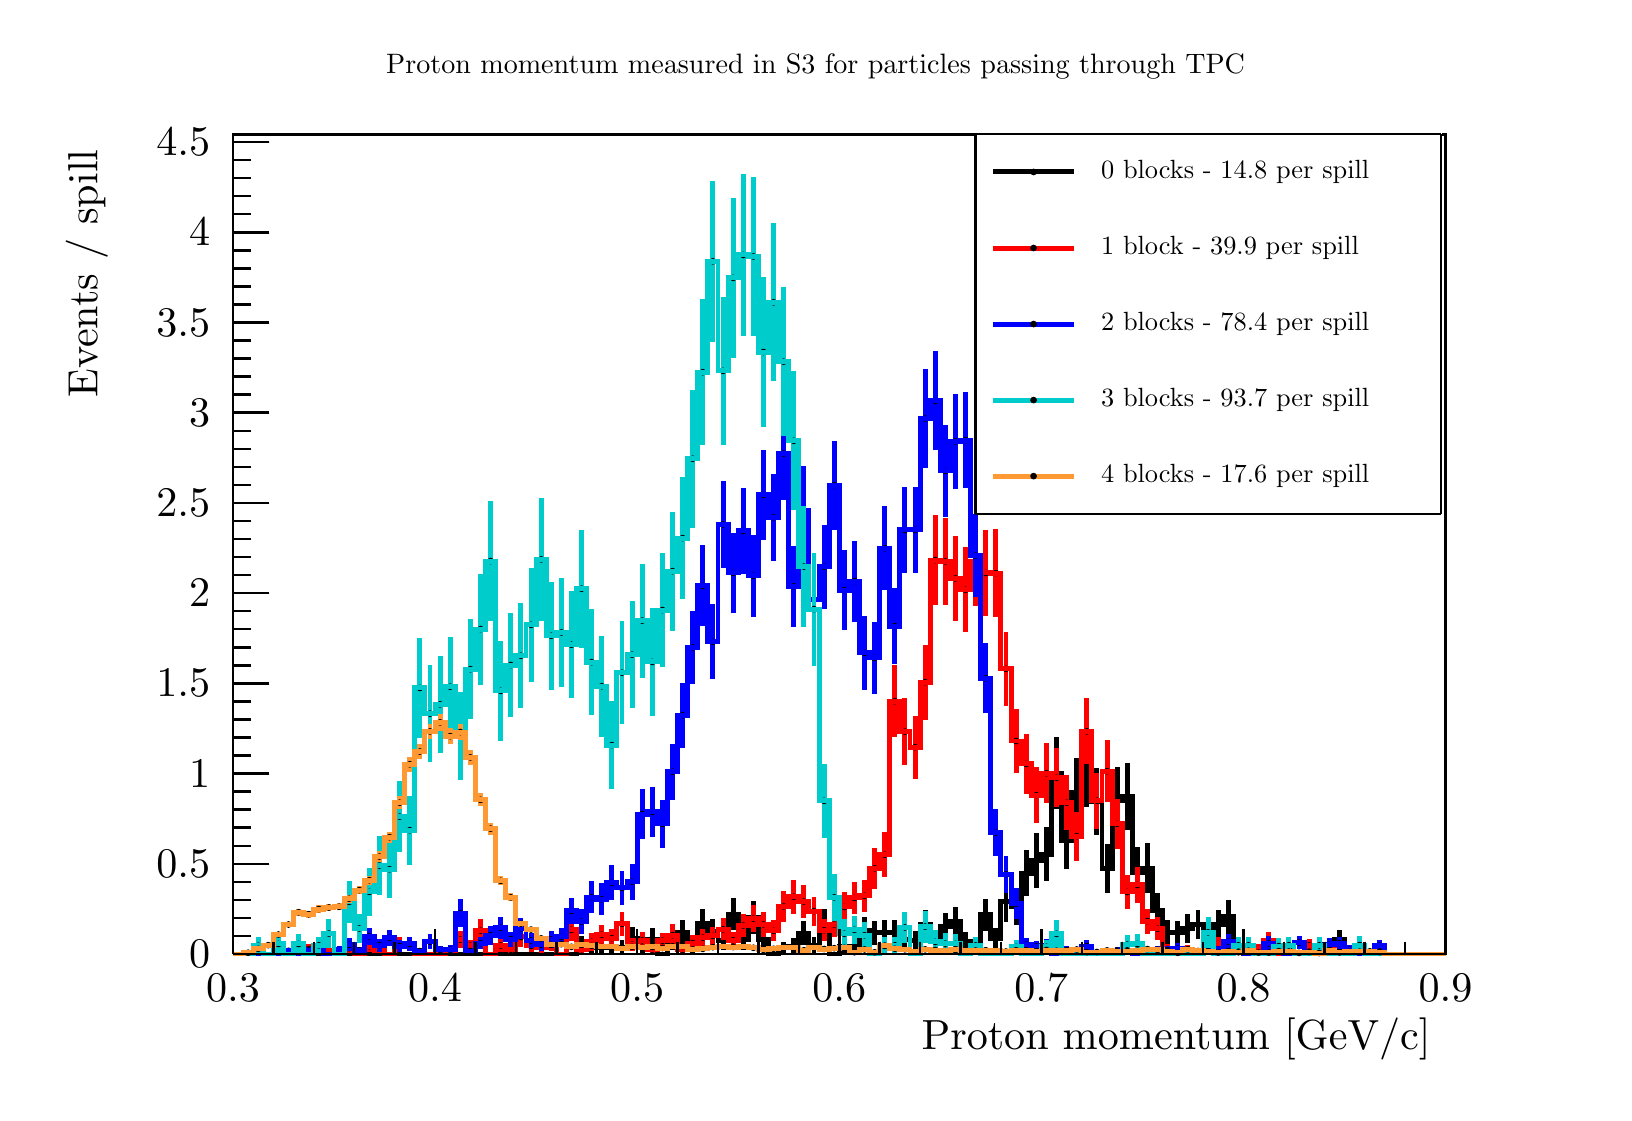
\begin{tikzpicture}
\pgfdeclareplotmark{cross} {
\pgfpathmoveto{\pgfpoint{-0.3\pgfplotmarksize}{\pgfplotmarksize}}
\pgfpathlineto{\pgfpoint{+0.3\pgfplotmarksize}{\pgfplotmarksize}}
\pgfpathlineto{\pgfpoint{+0.3\pgfplotmarksize}{0.3\pgfplotmarksize}}
\pgfpathlineto{\pgfpoint{+1\pgfplotmarksize}{0.3\pgfplotmarksize}}
\pgfpathlineto{\pgfpoint{+1\pgfplotmarksize}{-0.3\pgfplotmarksize}}
\pgfpathlineto{\pgfpoint{+0.3\pgfplotmarksize}{-0.3\pgfplotmarksize}}
\pgfpathlineto{\pgfpoint{+0.3\pgfplotmarksize}{-1.\pgfplotmarksize}}
\pgfpathlineto{\pgfpoint{-0.3\pgfplotmarksize}{-1.\pgfplotmarksize}}
\pgfpathlineto{\pgfpoint{-0.3\pgfplotmarksize}{-0.3\pgfplotmarksize}}
\pgfpathlineto{\pgfpoint{-1.\pgfplotmarksize}{-0.3\pgfplotmarksize}}
\pgfpathlineto{\pgfpoint{-1.\pgfplotmarksize}{0.3\pgfplotmarksize}}
\pgfpathlineto{\pgfpoint{-0.3\pgfplotmarksize}{0.3\pgfplotmarksize}}
\pgfpathclose
\pgfusepathqstroke
}
\pgfdeclareplotmark{cross*} {
\pgfpathmoveto{\pgfpoint{-0.3\pgfplotmarksize}{\pgfplotmarksize}}
\pgfpathlineto{\pgfpoint{+0.3\pgfplotmarksize}{\pgfplotmarksize}}
\pgfpathlineto{\pgfpoint{+0.3\pgfplotmarksize}{0.3\pgfplotmarksize}}
\pgfpathlineto{\pgfpoint{+1\pgfplotmarksize}{0.3\pgfplotmarksize}}
\pgfpathlineto{\pgfpoint{+1\pgfplotmarksize}{-0.3\pgfplotmarksize}}
\pgfpathlineto{\pgfpoint{+0.3\pgfplotmarksize}{-0.3\pgfplotmarksize}}
\pgfpathlineto{\pgfpoint{+0.3\pgfplotmarksize}{-1.\pgfplotmarksize}}
\pgfpathlineto{\pgfpoint{-0.3\pgfplotmarksize}{-1.\pgfplotmarksize}}
\pgfpathlineto{\pgfpoint{-0.3\pgfplotmarksize}{-0.3\pgfplotmarksize}}
\pgfpathlineto{\pgfpoint{-1.\pgfplotmarksize}{-0.3\pgfplotmarksize}}
\pgfpathlineto{\pgfpoint{-1.\pgfplotmarksize}{0.3\pgfplotmarksize}}
\pgfpathlineto{\pgfpoint{-0.3\pgfplotmarksize}{0.3\pgfplotmarksize}}
\pgfpathclose
\pgfusepathqfillstroke
}
\pgfdeclareplotmark{newstar} {
\pgfpathmoveto{\pgfqpoint{0pt}{\pgfplotmarksize}}
\pgfpathlineto{\pgfqpointpolar{44}{0.5\pgfplotmarksize}}
\pgfpathlineto{\pgfqpointpolar{18}{\pgfplotmarksize}}
\pgfpathlineto{\pgfqpointpolar{-20}{0.5\pgfplotmarksize}}
\pgfpathlineto{\pgfqpointpolar{-54}{\pgfplotmarksize}}
\pgfpathlineto{\pgfqpointpolar{-90}{0.5\pgfplotmarksize}}
\pgfpathlineto{\pgfqpointpolar{234}{\pgfplotmarksize}}
\pgfpathlineto{\pgfqpointpolar{198}{0.5\pgfplotmarksize}}
\pgfpathlineto{\pgfqpointpolar{162}{\pgfplotmarksize}}
\pgfpathlineto{\pgfqpointpolar{134}{0.5\pgfplotmarksize}}
\pgfpathclose
\pgfusepathqstroke
}
\pgfdeclareplotmark{newstar*} {
\pgfpathmoveto{\pgfqpoint{0pt}{\pgfplotmarksize}}
\pgfpathlineto{\pgfqpointpolar{44}{0.5\pgfplotmarksize}}
\pgfpathlineto{\pgfqpointpolar{18}{\pgfplotmarksize}}
\pgfpathlineto{\pgfqpointpolar{-20}{0.5\pgfplotmarksize}}
\pgfpathlineto{\pgfqpointpolar{-54}{\pgfplotmarksize}}
\pgfpathlineto{\pgfqpointpolar{-90}{0.5\pgfplotmarksize}}
\pgfpathlineto{\pgfqpointpolar{234}{\pgfplotmarksize}}
\pgfpathlineto{\pgfqpointpolar{198}{0.5\pgfplotmarksize}}
\pgfpathlineto{\pgfqpointpolar{162}{\pgfplotmarksize}}
\pgfpathlineto{\pgfqpointpolar{134}{0.5\pgfplotmarksize}}
\pgfpathclose
\pgfusepathqfillstroke
}
\definecolor{c}{rgb}{1,1,1};
\draw [color=c, fill=c] (0,0) rectangle (20,13.5143);
\draw [color=c, fill=c] (2.6,1.75686) rectangle (18,12.1629);
\definecolor{c}{rgb}{0,0,0};
\draw [c,line width=0.9] (2.6,1.75686) -- (2.6,12.1629) -- (18,12.1629) -- (18,1.75686) -- (2.6,1.75686);
\definecolor{c}{rgb}{1,1,1};
\draw [color=c, fill=c] (2.6,1.75686) rectangle (18,12.1629);
\definecolor{c}{rgb}{0,0,0};
\draw [c,line width=0.9] (2.6,1.75686) -- (2.6,12.1629) -- (18,12.1629) -- (18,1.75686) -- (2.6,1.75686);
\definecolor{c}{rgb}{0,0,0.6};
\draw [c,line width=0.9] (2.6,1.75686) -- (2.72833,1.75686) -- (2.72833,1.75686) -- (2.85667,1.75686) -- (2.85667,1.75686) -- (2.985,1.75686) -- (2.985,1.75686) -- (3.11333,1.75686) -- (3.11333,1.75686) -- (3.24167,1.75686) -- (3.24167,1.75686) --
 (3.37,1.75686) -- (3.37,1.75686) -- (3.49833,1.75686) -- (3.49833,1.75686) -- (3.62667,1.75686) -- (3.62667,1.75686) -- (3.755,1.75686) -- (3.755,1.75686) -- (3.88333,1.75686) -- (3.88333,1.75686) -- (4.01167,1.75686) -- (4.01167,1.75686) --
 (4.14,1.75686) -- (4.14,1.75686) -- (4.26833,1.75686) -- (4.26833,1.75686) -- (4.39667,1.75686) -- (4.39667,1.75686) -- (4.525,1.75686) -- (4.525,1.75686) -- (4.65333,1.75686) -- (4.65333,1.75686) -- (4.78167,1.75686) -- (4.78167,1.75686) --
 (4.91,1.75686) -- (4.91,1.75686) -- (5.03833,1.75686) -- (5.03833,1.75686) -- (5.16667,1.75686) -- (5.16667,1.75686) -- (5.295,1.75686) -- (5.295,1.75686) -- (5.42333,1.75686) -- (5.42333,1.75686) -- (5.55167,1.75686) -- (5.55167,1.75686) --
 (5.68,1.75686) -- (5.68,1.75686) -- (5.80833,1.75686) -- (5.80833,1.75686) -- (5.93667,1.75686) -- (5.93667,1.75686) -- (6.065,1.75686) -- (6.065,1.75686) -- (6.19333,1.75686) -- (6.19333,1.75686) -- (6.32167,1.75686) -- (6.32167,1.75686) --
 (6.45,1.75686) -- (6.45,1.75686) -- (6.57833,1.75686) -- (6.57833,1.75686) -- (6.70667,1.75686) -- (6.70667,1.75686) -- (6.835,1.75686) -- (6.835,1.75686) -- (6.96333,1.75686) -- (6.96333,1.75686) -- (7.09167,1.75686) -- (7.09167,1.75686) --
 (7.22,1.75686) -- (7.22,1.75686) -- (7.34833,1.75686) -- (7.34833,1.75686) -- (7.47667,1.75686) -- (7.47667,1.75686) -- (7.605,1.75686) -- (7.605,1.75686) -- (7.73333,1.75686) -- (7.73333,1.75686) -- (7.86167,1.75686) -- (7.86167,1.75686) --
 (7.99,1.75686) -- (7.99,1.75686) -- (8.11833,1.75686) -- (8.11833,1.75686) -- (8.24667,1.75686) -- (8.24667,1.75686) -- (8.375,1.75686) -- (8.375,1.75686) -- (8.50333,1.75686) -- (8.50333,1.75686) -- (8.63167,1.75686) -- (8.63167,1.75686) --
 (8.76,1.75686) -- (8.76,1.75686) -- (8.88833,1.75686) -- (8.88833,1.75686) -- (9.01667,1.75686) -- (9.01667,1.75686) -- (9.145,1.75686) -- (9.145,1.75686) -- (9.27333,1.75686) -- (9.27333,1.75686) -- (9.40167,1.75686) -- (9.40167,1.75686) --
 (9.53,1.75686) -- (9.53,1.75686) -- (9.65833,1.75686) -- (9.65833,1.75686) -- (9.78667,1.75686) -- (9.78667,1.75686) -- (9.915,1.75686) -- (9.915,1.75686) -- (10.0433,1.75686) -- (10.0433,1.75686) -- (10.1717,1.75686) -- (10.1717,1.75686) --
 (10.3,1.75686) -- (10.3,1.75686) -- (10.4283,1.75686) -- (10.4283,1.75686) -- (10.5567,1.75686) -- (10.5567,1.75686) -- (10.685,1.75686) -- (10.685,1.75686) -- (10.8133,1.75686) -- (10.8133,1.75686) -- (10.9417,1.75686) -- (10.9417,1.75686) --
 (11.07,1.75686) -- (11.07,1.75686) -- (11.1983,1.75686) -- (11.1983,1.75686) -- (11.3267,1.75686) -- (11.3267,1.75686) -- (11.455,1.75686) -- (11.455,1.75686) -- (11.5833,1.75686) -- (11.5833,1.75686) -- (11.7117,1.75686) -- (11.7117,1.75686) --
 (11.84,1.75686) -- (11.84,1.75686) -- (11.9683,1.75686) -- (11.9683,1.75686) -- (12.0967,1.75686) -- (12.0967,1.75686) -- (12.225,1.75686) -- (12.225,1.75686) -- (12.3533,1.75686) -- (12.3533,1.75686) -- (12.4817,1.75686) -- (12.4817,1.75686) --
 (12.61,1.75686) -- (12.61,1.75686) -- (12.7383,1.75686) -- (12.7383,1.75686) -- (12.8667,1.75686) -- (12.8667,1.75686) -- (12.995,1.75686) -- (12.995,1.75686) -- (13.1233,1.75686) -- (13.1233,1.75686) -- (13.2517,1.75686) -- (13.2517,1.75686) --
 (13.38,1.75686) -- (13.38,1.75686) -- (13.5083,1.75686) -- (13.5083,1.75686) -- (13.6367,1.75686) -- (13.6367,1.75686) -- (13.765,1.75686) -- (13.765,1.75686) -- (13.8933,1.75686) -- (13.8933,1.75686) -- (14.0217,1.75686) -- (14.0217,1.75686) --
 (14.15,1.75686) -- (14.15,1.75686) -- (14.2783,1.75686) -- (14.2783,1.75686) -- (14.4067,1.75686) -- (14.4067,1.75686) -- (14.535,1.75686) -- (14.535,1.75686) -- (14.6633,1.75686) -- (14.6633,1.75686) -- (14.7917,1.75686) -- (14.7917,1.75686) --
 (14.92,1.75686) -- (14.92,1.75686) -- (15.0483,1.75686) -- (15.0483,1.75686) -- (15.1767,1.75686) -- (15.1767,1.75686) -- (15.305,1.75686) -- (15.305,1.75686) -- (15.4333,1.75686) -- (15.4333,1.75686) -- (15.5617,1.75686) -- (15.5617,1.75686) --
 (15.69,1.75686) -- (15.69,1.75686) -- (15.8183,1.75686) -- (15.8183,1.75686) -- (15.9467,1.75686) -- (15.9467,1.75686) -- (16.075,1.75686) -- (16.075,1.75686) -- (16.2033,1.75686) -- (16.2033,1.75686) -- (16.3317,1.75686) -- (16.3317,1.75686) --
 (16.46,1.75686) -- (16.46,1.75686) -- (16.5883,1.75686) -- (16.5883,1.75686) -- (16.7167,1.75686) -- (16.7167,1.75686) -- (16.845,1.75686) -- (16.845,1.75686) -- (16.9733,1.75686) -- (16.9733,1.75686) -- (17.1017,1.75686) -- (17.1017,1.75686) --
 (17.23,1.75686) -- (17.23,1.75686) -- (17.3583,1.75686) -- (17.3583,1.75686) -- (17.4867,1.75686) -- (17.4867,1.75686) -- (17.615,1.75686) -- (17.615,1.75686) -- (17.7433,1.75686) -- (17.7433,1.75686) -- (17.8717,1.75686) -- (17.8717,1.75686) --
 (18,1.75686);
\definecolor{c}{rgb}{0,0,0};
\draw [c,line width=0.9] (2.6,1.75686) -- (18,1.75686);
\draw [c,line width=0.9] (2.6,2.06904) -- (2.6,1.75686);
\draw [c,line width=0.9] (3.11333,1.91295) -- (3.11333,1.75686);
\draw [c,line width=0.9] (3.62667,1.91295) -- (3.62667,1.75686);
\draw [c,line width=0.9] (4.14,1.91295) -- (4.14,1.75686);
\draw [c,line width=0.9] (4.65333,1.91295) -- (4.65333,1.75686);
\draw [c,line width=0.9] (5.16667,2.06904) -- (5.16667,1.75686);
\draw [c,line width=0.9] (5.68,1.91295) -- (5.68,1.75686);
\draw [c,line width=0.9] (6.19333,1.91295) -- (6.19333,1.75686);
\draw [c,line width=0.9] (6.70667,1.91295) -- (6.70667,1.75686);
\draw [c,line width=0.9] (7.22,1.91295) -- (7.22,1.75686);
\draw [c,line width=0.9] (7.73333,2.06904) -- (7.73333,1.75686);
\draw [c,line width=0.9] (8.24667,1.91295) -- (8.24667,1.75686);
\draw [c,line width=0.9] (8.76,1.91295) -- (8.76,1.75686);
\draw [c,line width=0.9] (9.27333,1.91295) -- (9.27333,1.75686);
\draw [c,line width=0.9] (9.78667,1.91295) -- (9.78667,1.75686);
\draw [c,line width=0.9] (10.3,2.06904) -- (10.3,1.75686);
\draw [c,line width=0.9] (10.8133,1.91295) -- (10.8133,1.75686);
\draw [c,line width=0.9] (11.3267,1.91295) -- (11.3267,1.75686);
\draw [c,line width=0.9] (11.84,1.91295) -- (11.84,1.75686);
\draw [c,line width=0.9] (12.3533,1.91295) -- (12.3533,1.75686);
\draw [c,line width=0.9] (12.8667,2.06904) -- (12.8667,1.75686);
\draw [c,line width=0.9] (13.38,1.91295) -- (13.38,1.75686);
\draw [c,line width=0.9] (13.8933,1.91295) -- (13.8933,1.75686);
\draw [c,line width=0.9] (14.4067,1.91295) -- (14.4067,1.75686);
\draw [c,line width=0.9] (14.92,1.91295) -- (14.92,1.75686);
\draw [c,line width=0.9] (15.4333,2.06904) -- (15.4333,1.75686);
\draw [c,line width=0.9] (15.9467,1.91295) -- (15.9467,1.75686);
\draw [c,line width=0.9] (16.46,1.91295) -- (16.46,1.75686);
\draw [c,line width=0.9] (16.9733,1.91295) -- (16.9733,1.75686);
\draw [c,line width=0.9] (17.4867,1.91295) -- (17.4867,1.75686);
\draw [c,line width=0.9] (18,2.06904) -- (18,1.75686);
\draw [c,line width=0.9] (2.6,2.06904) -- (2.6,1.75686);
\draw [c,line width=0.9] (18,2.06904) -- (18,1.75686);
\draw [anchor=base] (2.6,1.14871) node[scale=1.52295, color=c, rotate=0]{0.3};
\draw [anchor=base] (5.16667,1.14871) node[scale=1.52295, color=c, rotate=0]{0.4};
\draw [anchor=base] (7.73333,1.14871) node[scale=1.52295, color=c, rotate=0]{0.5};
\draw [anchor=base] (10.3,1.14871) node[scale=1.52295, color=c, rotate=0]{0.6};
\draw [anchor=base] (12.8667,1.14871) node[scale=1.52295, color=c, rotate=0]{0.7};
\draw [anchor=base] (15.4333,1.14871) node[scale=1.52295, color=c, rotate=0]{0.8};
\draw [anchor=base] (18,1.14871) node[scale=1.52295, color=c, rotate=0]{0.9};
\draw [anchor= east] (18,0.675714) node[scale=1.52295, color=c, rotate=0]{ Proton momentum [GeV/c]};
\draw [c,line width=0.9] (2.6,1.75686) -- (2.6,12.1629);
\draw [c,line width=0.9] (3.062,1.75686) -- (2.6,1.75686);
\draw [c,line width=0.9] (2.831,1.986) -- (2.6,1.986);
\draw [c,line width=0.9] (2.831,2.21514) -- (2.6,2.21514);
\draw [c,line width=0.9] (2.831,2.44429) -- (2.6,2.44429);
\draw [c,line width=0.9] (2.831,2.67343) -- (2.6,2.67343);
\draw [c,line width=0.9] (3.062,2.90257) -- (2.6,2.90257);
\draw [c,line width=0.9] (2.831,3.13171) -- (2.6,3.13171);
\draw [c,line width=0.9] (2.831,3.36086) -- (2.6,3.36086);
\draw [c,line width=0.9] (2.831,3.59) -- (2.6,3.59);
\draw [c,line width=0.9] (2.831,3.81914) -- (2.6,3.81914);
\draw [c,line width=0.9] (3.062,4.04829) -- (2.6,4.04829);
\draw [c,line width=0.9] (2.831,4.27743) -- (2.6,4.27743);
\draw [c,line width=0.9] (2.831,4.50657) -- (2.6,4.50657);
\draw [c,line width=0.9] (2.831,4.73572) -- (2.6,4.73572);
\draw [c,line width=0.9] (2.831,4.96486) -- (2.6,4.96486);
\draw [c,line width=0.9] (3.062,5.194) -- (2.6,5.194);
\draw [c,line width=0.9] (2.831,5.42314) -- (2.6,5.42314);
\draw [c,line width=0.9] (2.831,5.65229) -- (2.6,5.65229);
\draw [c,line width=0.9] (2.831,5.88143) -- (2.6,5.88143);
\draw [c,line width=0.9] (2.831,6.11057) -- (2.6,6.11057);
\draw [c,line width=0.9] (3.062,6.33972) -- (2.6,6.33972);
\draw [c,line width=0.9] (2.831,6.56886) -- (2.6,6.56886);
\draw [c,line width=0.9] (2.831,6.798) -- (2.6,6.798);
\draw [c,line width=0.9] (2.831,7.02714) -- (2.6,7.02714);
\draw [c,line width=0.9] (2.831,7.25629) -- (2.6,7.25629);
\draw [c,line width=0.9] (3.062,7.48543) -- (2.6,7.48543);
\draw [c,line width=0.9] (2.831,7.71457) -- (2.6,7.71457);
\draw [c,line width=0.9] (2.831,7.94372) -- (2.6,7.94372);
\draw [c,line width=0.9] (2.831,8.17286) -- (2.6,8.17286);
\draw [c,line width=0.9] (2.831,8.402) -- (2.6,8.402);
\draw [c,line width=0.9] (3.062,8.63114) -- (2.6,8.63114);
\draw [c,line width=0.9] (2.831,8.86029) -- (2.6,8.86029);
\draw [c,line width=0.9] (2.831,9.08943) -- (2.6,9.08943);
\draw [c,line width=0.9] (2.831,9.31857) -- (2.6,9.31857);
\draw [c,line width=0.9] (2.831,9.54772) -- (2.6,9.54772);
\draw [c,line width=0.9] (3.062,9.77686) -- (2.6,9.77686);
\draw [c,line width=0.9] (2.831,10.006) -- (2.6,10.006);
\draw [c,line width=0.9] (2.831,10.2351) -- (2.6,10.2351);
\draw [c,line width=0.9] (2.831,10.4643) -- (2.6,10.4643);
\draw [c,line width=0.9] (2.831,10.6934) -- (2.6,10.6934);
\draw [c,line width=0.9] (3.062,10.9226) -- (2.6,10.9226);
\draw [c,line width=0.9] (2.831,11.1517) -- (2.6,11.1517);
\draw [c,line width=0.9] (2.831,11.3809) -- (2.6,11.3809);
\draw [c,line width=0.9] (2.831,11.61) -- (2.6,11.61);
\draw [c,line width=0.9] (2.831,11.8391) -- (2.6,11.8391);
\draw [c,line width=0.9] (3.062,12.0683) -- (2.6,12.0683);
\draw [c,line width=0.9] (3.062,12.0683) -- (2.6,12.0683);
\draw [anchor= east] (2.5,1.75686) node[scale=1.52295, color=c, rotate=0]{0};
\draw [anchor= east] (2.5,2.90257) node[scale=1.52295, color=c, rotate=0]{0.5};
\draw [anchor= east] (2.5,4.04829) node[scale=1.52295, color=c, rotate=0]{1};
\draw [anchor= east] (2.5,5.194) node[scale=1.52295, color=c, rotate=0]{1.5};
\draw [anchor= east] (2.5,6.33972) node[scale=1.52295, color=c, rotate=0]{2};
\draw [anchor= east] (2.5,7.48543) node[scale=1.52295, color=c, rotate=0]{2.5};
\draw [anchor= east] (2.5,8.63114) node[scale=1.52295, color=c, rotate=0]{3};
\draw [anchor= east] (2.5,9.77686) node[scale=1.52295, color=c, rotate=0]{3.5};
\draw [anchor= east] (2.5,10.9226) node[scale=1.52295, color=c, rotate=0]{4};
\draw [anchor= east] (2.5,12.0683) node[scale=1.52295, color=c, rotate=0]{4.5};
\draw [anchor= east] (0.742857,12.1629) node[scale=1.52295, color=c, rotate=90]{ Events / spill};
\draw [c,line width=1.8] (7.0275,1.75686) -- (7.0275,1.87223);
\draw [c,line width=1.8] (7.0275,1.87223) -- (7.0275,1.98761);
\foreach \P in {(7.0275,1.87223)}{\draw[mark options={color=c,fill=c},mark size=2.402402pt,mark=*,mark size=1pt] plot coordinates {\P};}
\draw [c,line width=1.8] (7.15583,1.75686) -- (7.15583,1.8392);
\draw [c,line width=1.8] (7.15583,1.8392) -- (7.15583,1.92154);
\foreach \P in {(7.15583,1.8392)}{\draw[mark options={color=c,fill=c},mark size=2.402402pt,mark=*,mark size=1pt] plot coordinates {\P};}
\draw [c,line width=1.8] (7.28417,1.75686) -- (7.28417,1.84002);
\draw [c,line width=1.8] (7.28417,1.84002) -- (7.28417,1.92318);
\foreach \P in {(7.28417,1.84002)}{\draw[mark options={color=c,fill=c},mark size=2.402402pt,mark=*,mark size=1pt] plot coordinates {\P};}
\draw [c,line width=1.8] (7.4125,1.75686) -- (7.4125,1.84723);
\draw [c,line width=1.8] (7.4125,1.84723) -- (7.4125,1.9376);
\foreach \P in {(7.4125,1.84723)}{\draw[mark options={color=c,fill=c},mark size=2.402402pt,mark=*,mark size=1pt] plot coordinates {\P};}
\draw [c,line width=1.8] (7.54083,1.75686) -- (7.54083,1.84318);
\draw [c,line width=1.8] (7.54083,1.84318) -- (7.54083,1.9295);
\foreach \P in {(7.54083,1.84318)}{\draw[mark options={color=c,fill=c},mark size=2.402402pt,mark=*,mark size=1pt] plot coordinates {\P};}
\draw [c,line width=1.8] (7.66917,1.81491) -- (7.66917,1.95785);
\draw [c,line width=1.8] (7.66917,1.95785) -- (7.66917,2.10079);
\foreach \P in {(7.66917,1.95785)}{\draw[mark options={color=c,fill=c},mark size=2.402402pt,mark=*,mark size=1pt] plot coordinates {\P};}
\draw [c,line width=1.8] (7.7975,1.75686) -- (7.7975,1.84723);
\draw [c,line width=1.8] (7.7975,1.84723) -- (7.7975,1.9376);
\foreach \P in {(7.7975,1.84723)}{\draw[mark options={color=c,fill=c},mark size=2.402402pt,mark=*,mark size=1pt] plot coordinates {\P};}
\draw [c,line width=1.8] (7.92583,1.8114) -- (7.92583,1.94655);
\draw [c,line width=1.8] (7.92583,1.94655) -- (7.92583,2.0817);
\foreach \P in {(7.92583,1.94655)}{\draw[mark options={color=c,fill=c},mark size=2.402402pt,mark=*,mark size=1pt] plot coordinates {\P};}
\draw [c,line width=1.8] (8.1825,1.80673) -- (8.1825,1.92724);
\draw [c,line width=1.8] (8.1825,1.92724) -- (8.1825,2.04776);
\foreach \P in {(8.1825,1.92724)}{\draw[mark options={color=c,fill=c},mark size=2.402402pt,mark=*,mark size=1pt] plot coordinates {\P};}
\draw [c,line width=1.8] (8.31083,1.87249) -- (8.31083,2.03228);
\draw [c,line width=1.8] (8.31083,2.03228) -- (8.31083,2.19207);
\foreach \P in {(8.31083,2.03228)}{\draw[mark options={color=c,fill=c},mark size=2.402402pt,mark=*,mark size=1pt] plot coordinates {\P};}
\draw [c,line width=1.8] (8.43917,1.75686) -- (8.43917,1.84992);
\draw [c,line width=1.8] (8.43917,1.84992) -- (8.43917,1.94298);
\foreach \P in {(8.43917,1.84992)}{\draw[mark options={color=c,fill=c},mark size=2.402402pt,mark=*,mark size=1pt] plot coordinates {\P};}
\draw [c,line width=1.8] (8.5675,1.94739) -- (8.5675,2.14072);
\draw [c,line width=1.8] (8.5675,2.14072) -- (8.5675,2.33405);
\foreach \P in {(8.5675,2.14072)}{\draw[mark options={color=c,fill=c},mark size=2.402402pt,mark=*,mark size=1pt] plot coordinates {\P};}
\draw [c,line width=1.8] (8.69583,1.87635) -- (8.69583,2.04052);
\draw [c,line width=1.8] (8.69583,2.04052) -- (8.69583,2.20468);
\foreach \P in {(8.69583,2.04052)}{\draw[mark options={color=c,fill=c},mark size=2.402402pt,mark=*,mark size=1pt] plot coordinates {\P};}
\draw [c,line width=1.8] (8.82417,1.80664) -- (8.82417,1.92697);
\draw [c,line width=1.8] (8.82417,1.92697) -- (8.82417,2.04729);
\foreach \P in {(8.82417,1.92697)}{\draw[mark options={color=c,fill=c},mark size=2.402402pt,mark=*,mark size=1pt] plot coordinates {\P};}
\draw [c,line width=1.8] (8.9525,2.05573) -- (8.9525,2.26287);
\draw [c,line width=1.8] (8.9525,2.26287) -- (8.9525,2.47002);
\foreach \P in {(8.9525,2.26287)}{\draw[mark options={color=c,fill=c},mark size=2.402402pt,mark=*,mark size=1pt] plot coordinates {\P};}
\draw [c,line width=1.8] (9.08083,1.81125) -- (9.08083,1.94304);
\draw [c,line width=1.8] (9.08083,1.94304) -- (9.08083,2.07483);
\foreach \P in {(9.08083,1.94304)}{\draw[mark options={color=c,fill=c},mark size=2.402402pt,mark=*,mark size=1pt] plot coordinates {\P};}
\draw [c,line width=1.8] (9.20917,2.01159) -- (9.20917,2.21923);
\draw [c,line width=1.8] (9.20917,2.21923) -- (9.20917,2.42687);
\foreach \P in {(9.20917,2.21923)}{\draw[mark options={color=c,fill=c},mark size=2.402402pt,mark=*,mark size=1pt] plot coordinates {\P};}
\draw [c,line width=1.8] (9.3375,1.80986) -- (9.3375,1.93843);
\draw [c,line width=1.8] (9.3375,1.93843) -- (9.3375,2.067);
\foreach \P in {(9.3375,1.93843)}{\draw[mark options={color=c,fill=c},mark size=2.402402pt,mark=*,mark size=1pt] plot coordinates {\P};}
\draw [c,line width=1.8] (9.59417,1.75686) -- (9.59417,1.83459);
\draw [c,line width=1.8] (9.59417,1.83459) -- (9.59417,1.91233);
\foreach \P in {(9.59417,1.83459)}{\draw[mark options={color=c,fill=c},mark size=2.402402pt,mark=*,mark size=1pt] plot coordinates {\P};}
\draw [c,line width=1.8] (9.7225,1.75686) -- (9.7225,1.8562);
\draw [c,line width=1.8] (9.7225,1.8562) -- (9.7225,1.95554);
\foreach \P in {(9.7225,1.8562)}{\draw[mark options={color=c,fill=c},mark size=2.402402pt,mark=*,mark size=1pt] plot coordinates {\P};}
\draw [c,line width=1.8] (9.85083,1.86877) -- (9.85083,2.02172);
\draw [c,line width=1.8] (9.85083,2.02172) -- (9.85083,2.17468);
\foreach \P in {(9.85083,2.02172)}{\draw[mark options={color=c,fill=c},mark size=2.402402pt,mark=*,mark size=1pt] plot coordinates {\P};}
\draw [c,line width=1.8] (9.97917,1.75686) -- (9.97917,1.86339);
\draw [c,line width=1.8] (9.97917,1.86339) -- (9.97917,1.96992);
\foreach \P in {(9.97917,1.86339)}{\draw[mark options={color=c,fill=c},mark size=2.402402pt,mark=*,mark size=1pt] plot coordinates {\P};}
\draw [c,line width=1.8] (10.1075,1.94483) -- (10.1075,2.13416);
\draw [c,line width=1.8] (10.1075,2.13416) -- (10.1075,2.32349);
\foreach \P in {(10.1075,2.13416)}{\draw[mark options={color=c,fill=c},mark size=2.402402pt,mark=*,mark size=1pt] plot coordinates {\P};}
\draw [c,line width=1.8] (10.3642,1.75686) -- (10.3642,1.85132);
\draw [c,line width=1.8] (10.3642,1.85132) -- (10.3642,1.94579);
\foreach \P in {(10.3642,1.85132)}{\draw[mark options={color=c,fill=c},mark size=2.402402pt,mark=*,mark size=1pt] plot coordinates {\P};}
\draw [c,line width=1.8] (10.4925,1.75686) -- (10.4925,1.83893);
\draw [c,line width=1.8] (10.4925,1.83893) -- (10.4925,1.921);
\foreach \P in {(10.4925,1.83893)}{\draw[mark options={color=c,fill=c},mark size=2.402402pt,mark=*,mark size=1pt] plot coordinates {\P};}
\draw [c,line width=1.8] (10.6208,1.88288) -- (10.6208,2.05538);
\draw [c,line width=1.8] (10.6208,2.05538) -- (10.6208,2.22788);
\foreach \P in {(10.6208,2.05538)}{\draw[mark options={color=c,fill=c},mark size=2.402402pt,mark=*,mark size=1pt] plot coordinates {\P};}
\draw [c,line width=1.8] (10.7492,1.87023) -- (10.7492,2.02579);
\draw [c,line width=1.8] (10.7492,2.02579) -- (10.7492,2.18135);
\foreach \P in {(10.7492,2.02579)}{\draw[mark options={color=c,fill=c},mark size=2.402402pt,mark=*,mark size=1pt] plot coordinates {\P};}
\draw [c,line width=1.8] (10.8775,1.87276) -- (10.8775,2.03138);
\draw [c,line width=1.8] (10.8775,2.03138) -- (10.8775,2.19001);
\foreach \P in {(10.8775,2.03138)}{\draw[mark options={color=c,fill=c},mark size=2.402402pt,mark=*,mark size=1pt] plot coordinates {\P};}
\draw [c,line width=1.8] (11.0058,1.87083) -- (11.0058,2.02682);
\draw [c,line width=1.8] (11.0058,2.02682) -- (11.0058,2.18281);
\foreach \P in {(11.0058,2.02682)}{\draw[mark options={color=c,fill=c},mark size=2.402402pt,mark=*,mark size=1pt] plot coordinates {\P};}
\draw [c,line width=1.8] (11.1342,1.81209) -- (11.1342,1.94544);
\draw [c,line width=1.8] (11.1342,1.94544) -- (11.1342,2.07878);
\foreach \P in {(11.1342,1.94544)}{\draw[mark options={color=c,fill=c},mark size=2.402402pt,mark=*,mark size=1pt] plot coordinates {\P};}
\draw [c,line width=1.8] (11.2625,1.80748) -- (11.2625,1.93029);
\draw [c,line width=1.8] (11.2625,1.93029) -- (11.2625,2.0531);
\foreach \P in {(11.2625,1.93029)}{\draw[mark options={color=c,fill=c},mark size=2.402402pt,mark=*,mark size=1pt] plot coordinates {\P};}
\draw [c,line width=1.8] (11.3908,1.94375) -- (11.3908,2.13179);
\draw [c,line width=1.8] (11.3908,2.13179) -- (11.3908,2.31983);
\foreach \P in {(11.3908,2.13179)}{\draw[mark options={color=c,fill=c},mark size=2.402402pt,mark=*,mark size=1pt] plot coordinates {\P};}
\draw [c,line width=1.8] (11.5192,1.80584) -- (11.5192,1.92521);
\draw [c,line width=1.8] (11.5192,1.92521) -- (11.5192,2.04457);
\foreach \P in {(11.5192,1.92521)}{\draw[mark options={color=c,fill=c},mark size=2.402402pt,mark=*,mark size=1pt] plot coordinates {\P};}
\draw [c,line width=1.8] (11.6475,1.93039) -- (11.6475,2.10696);
\draw [c,line width=1.8] (11.6475,2.10696) -- (11.6475,2.28353);
\foreach \P in {(11.6475,2.10696)}{\draw[mark options={color=c,fill=c},mark size=2.402402pt,mark=*,mark size=1pt] plot coordinates {\P};}
\draw [c,line width=1.8] (11.7758,1.98331) -- (11.7758,2.16693);
\draw [c,line width=1.8] (11.7758,2.16693) -- (11.7758,2.35054);
\foreach \P in {(11.7758,2.16693)}{\draw[mark options={color=c,fill=c},mark size=2.402402pt,mark=*,mark size=1pt] plot coordinates {\P};}
\draw [c,line width=1.8] (11.9042,1.80478) -- (11.9042,1.92049);
\draw [c,line width=1.8] (11.9042,1.92049) -- (11.9042,2.03621);
\foreach \P in {(11.9042,1.92049)}{\draw[mark options={color=c,fill=c},mark size=2.402402pt,mark=*,mark size=1pt] plot coordinates {\P};}
\draw [c,line width=1.8] (12.0325,1.75686) -- (12.0325,1.84469);
\draw [c,line width=1.8] (12.0325,1.84469) -- (12.0325,1.93253);
\foreach \P in {(12.0325,1.84469)}{\draw[mark options={color=c,fill=c},mark size=2.402402pt,mark=*,mark size=1pt] plot coordinates {\P};}
\draw [c,line width=1.8] (12.1608,2.051) -- (12.1608,2.25481);
\draw [c,line width=1.8] (12.1608,2.25481) -- (12.1608,2.45862);
\foreach \P in {(12.1608,2.25481)}{\draw[mark options={color=c,fill=c},mark size=2.402402pt,mark=*,mark size=1pt] plot coordinates {\P};}
\draw [c,line width=1.8] (12.2892,1.81436) -- (12.2892,1.95325);
\draw [c,line width=1.8] (12.2892,1.95325) -- (12.2892,2.09214);
\foreach \P in {(12.2892,1.95325)}{\draw[mark options={color=c,fill=c},mark size=2.402402pt,mark=*,mark size=1pt] plot coordinates {\P};}
\draw [c,line width=1.8] (12.4175,2.16918) -- (12.4175,2.42216);
\draw [c,line width=1.8] (12.4175,2.42216) -- (12.4175,2.67513);
\foreach \P in {(12.4175,2.42216)}{\draw[mark options={color=c,fill=c},mark size=2.402402pt,mark=*,mark size=1pt] plot coordinates {\P};}
\draw [c,line width=1.8] (12.5458,2.12973) -- (12.5458,2.35702);
\draw [c,line width=1.8] (12.5458,2.35702) -- (12.5458,2.58431);
\foreach \P in {(12.5458,2.35702)}{\draw[mark options={color=c,fill=c},mark size=2.402402pt,mark=*,mark size=1pt] plot coordinates {\P};}
\draw [c,line width=1.8] (12.6742,2.48745) -- (12.6742,2.78505);
\draw [c,line width=1.8] (12.6742,2.78505) -- (12.6742,3.08264);
\foreach \P in {(12.6742,2.78505)}{\draw[mark options={color=c,fill=c},mark size=2.402402pt,mark=*,mark size=1pt] plot coordinates {\P};}
\draw [c,line width=1.8] (12.8025,2.60099) -- (12.8025,2.9455);
\draw [c,line width=1.8] (12.8025,2.9455) -- (12.8025,3.29001);
\foreach \P in {(12.8025,2.9455)}{\draw[mark options={color=c,fill=c},mark size=2.402402pt,mark=*,mark size=1pt] plot coordinates {\P};}
\draw [c,line width=1.8] (12.9308,2.68361) -- (12.9308,3.02538);
\draw [c,line width=1.8] (12.9308,3.02538) -- (12.9308,3.36715);
\foreach \P in {(12.9308,3.02538)}{\draw[mark options={color=c,fill=c},mark size=2.402402pt,mark=*,mark size=1pt] plot coordinates {\P};}
\draw [c,line width=1.8] (13.0592,3.59301) -- (13.0592,4.05439);
\draw [c,line width=1.8] (13.0592,4.05439) -- (13.0592,4.51577);
\foreach \P in {(13.0592,4.05439)}{\draw[mark options={color=c,fill=c},mark size=2.402402pt,mark=*,mark size=1pt] plot coordinates {\P};}
\draw [c,line width=1.8] (13.1875,2.83168) -- (13.1875,3.19282);
\draw [c,line width=1.8] (13.1875,3.19282) -- (13.1875,3.55396);
\foreach \P in {(13.1875,3.19282)}{\draw[mark options={color=c,fill=c},mark size=2.402402pt,mark=*,mark size=1pt] plot coordinates {\P};}
\draw [c,line width=1.8] (13.3158,3.36598) -- (13.3158,3.80513);
\draw [c,line width=1.8] (13.3158,3.80513) -- (13.3158,4.24429);
\foreach \P in {(13.3158,3.80513)}{\draw[mark options={color=c,fill=c},mark size=2.402402pt,mark=*,mark size=1pt] plot coordinates {\P};}
\draw [c,line width=1.8] (13.4442,3.62133) -- (13.4442,4.0904);
\draw [c,line width=1.8] (13.4442,4.0904) -- (13.4442,4.55947);
\foreach \P in {(13.4442,4.0904)}{\draw[mark options={color=c,fill=c},mark size=2.402402pt,mark=*,mark size=1pt] plot coordinates {\P};}
\draw [c,line width=1.8] (13.5725,3.26516) -- (13.5725,3.68928);
\draw [c,line width=1.8] (13.5725,3.68928) -- (13.5725,4.1134);
\foreach \P in {(13.5725,3.68928)}{\draw[mark options={color=c,fill=c},mark size=2.402402pt,mark=*,mark size=1pt] plot coordinates {\P};}
\draw [c,line width=1.8] (13.7008,2.53033) -- (13.7008,2.84511);
\draw [c,line width=1.8] (13.7008,2.84511) -- (13.7008,3.15989);
\foreach \P in {(13.7008,2.84511)}{\draw[mark options={color=c,fill=c},mark size=2.402402pt,mark=*,mark size=1pt] plot coordinates {\P};}
\draw [c,line width=1.8] (13.8292,3.28205) -- (13.8292,3.71001);
\draw [c,line width=1.8] (13.8292,3.71001) -- (13.8292,4.13798);
\foreach \P in {(13.8292,3.71001)}{\draw[mark options={color=c,fill=c},mark size=2.402402pt,mark=*,mark size=1pt] plot coordinates {\P};}
\draw [c,line width=1.8] (13.9575,3.32834) -- (13.9575,3.75732);
\draw [c,line width=1.8] (13.9575,3.75732) -- (13.9575,4.1863);
\foreach \P in {(13.9575,3.75732)}{\draw[mark options={color=c,fill=c},mark size=2.402402pt,mark=*,mark size=1pt] plot coordinates {\P};}
\draw [c,line width=1.8] (14.0858,2.4802) -- (14.0858,2.79644);
\draw [c,line width=1.8] (14.0858,2.79644) -- (14.0858,3.11269);
\foreach \P in {(14.0858,2.79644)}{\draw[mark options={color=c,fill=c},mark size=2.402402pt,mark=*,mark size=1pt] plot coordinates {\P};}
\draw [c,line width=1.8] (14.2142,2.53008) -- (14.2142,2.84544);
\draw [c,line width=1.8] (14.2142,2.84544) -- (14.2142,3.1608);
\foreach \P in {(14.2142,2.84544)}{\draw[mark options={color=c,fill=c},mark size=2.402402pt,mark=*,mark size=1pt] plot coordinates {\P};}
\draw [c,line width=1.8] (14.3425,2.08132) -- (14.3425,2.30593);
\draw [c,line width=1.8] (14.3425,2.30593) -- (14.3425,2.53053);
\foreach \P in {(14.3425,2.30593)}{\draw[mark options={color=c,fill=c},mark size=2.402402pt,mark=*,mark size=1pt] plot coordinates {\P};}
\draw [c,line width=1.8] (14.4708,1.87354) -- (14.4708,2.03359);
\draw [c,line width=1.8] (14.4708,2.03359) -- (14.4708,2.19363);
\foreach \P in {(14.4708,2.03359)}{\draw[mark options={color=c,fill=c},mark size=2.402402pt,mark=*,mark size=1pt] plot coordinates {\P};}
\draw [c,line width=1.8] (14.5992,1.86891) -- (14.5992,2.02386);
\draw [c,line width=1.8] (14.5992,2.02386) -- (14.5992,2.17881);
\foreach \P in {(14.5992,2.02386)}{\draw[mark options={color=c,fill=c},mark size=2.402402pt,mark=*,mark size=1pt] plot coordinates {\P};}
\draw [c,line width=1.8] (14.7275,1.89144) -- (14.7275,2.07855);
\draw [c,line width=1.8] (14.7275,2.07855) -- (14.7275,2.26565);
\foreach \P in {(14.7275,2.07855)}{\draw[mark options={color=c,fill=c},mark size=2.402402pt,mark=*,mark size=1pt] plot coordinates {\P};}
\draw [c,line width=1.8] (14.8558,1.94316) -- (14.8558,2.13117);
\draw [c,line width=1.8] (14.8558,2.13117) -- (14.8558,2.31917);
\foreach \P in {(14.8558,2.13117)}{\draw[mark options={color=c,fill=c},mark size=2.402402pt,mark=*,mark size=1pt] plot coordinates {\P};}
\draw [c,line width=1.8] (14.9842,1.88047) -- (14.9842,2.04993);
\draw [c,line width=1.8] (14.9842,2.04993) -- (14.9842,2.21939);
\foreach \P in {(14.9842,2.04993)}{\draw[mark options={color=c,fill=c},mark size=2.402402pt,mark=*,mark size=1pt] plot coordinates {\P};}
\draw [c,line width=1.8] (15.1125,1.94323) -- (15.1125,2.13173);
\draw [c,line width=1.8] (15.1125,2.13173) -- (15.1125,2.32023);
\foreach \P in {(15.1125,2.13173)}{\draw[mark options={color=c,fill=c},mark size=2.402402pt,mark=*,mark size=1pt] plot coordinates {\P};}
\draw [c,line width=1.8] (15.2408,2.01694) -- (15.2408,2.23066);
\draw [c,line width=1.8] (15.2408,2.23066) -- (15.2408,2.44439);
\foreach \P in {(15.2408,2.23066)}{\draw[mark options={color=c,fill=c},mark size=2.402402pt,mark=*,mark size=1pt] plot coordinates {\P};}
\draw [c,line width=1.8] (15.3692,1.75686) -- (15.3692,1.83893);
\draw [c,line width=1.8] (15.3692,1.83893) -- (15.3692,1.921);
\foreach \P in {(15.3692,1.83893)}{\draw[mark options={color=c,fill=c},mark size=2.402402pt,mark=*,mark size=1pt] plot coordinates {\P};}
\draw [c,line width=1.8] (16.0108,1.75686) -- (16.0108,1.8566);
\draw [c,line width=1.8] (16.0108,1.8566) -- (16.0108,1.95633);
\foreach \P in {(16.0108,1.8566)}{\draw[mark options={color=c,fill=c},mark size=2.402402pt,mark=*,mark size=1pt] plot coordinates {\P};}
\draw [c,line width=1.8] (16.3958,1.75686) -- (16.3958,1.83225);
\draw [c,line width=1.8] (16.3958,1.83225) -- (16.3958,1.90765);
\foreach \P in {(16.3958,1.83225)}{\draw[mark options={color=c,fill=c},mark size=2.402402pt,mark=*,mark size=1pt] plot coordinates {\P};}
\draw [c,line width=1.8] (16.6525,1.8092) -- (16.6525,1.93618);
\draw [c,line width=1.8] (16.6525,1.93618) -- (16.6525,2.06316);
\foreach \P in {(16.6525,1.93618)}{\draw[mark options={color=c,fill=c},mark size=2.402402pt,mark=*,mark size=1pt] plot coordinates {\P};}
\draw [c,line width=1.8] (16.9092,1.75686) -- (16.9092,1.86161);
\draw [c,line width=1.8] (16.9092,1.86161) -- (16.9092,1.96636);
\foreach \P in {(16.9092,1.86161)}{\draw[mark options={color=c,fill=c},mark size=2.402402pt,mark=*,mark size=1pt] plot coordinates {\P};}
\draw [c,line width=1.8] (2.6,1.75686) -- (2.72833,1.75686) -- (2.72833,1.75686) -- (2.85667,1.75686) -- (2.85667,1.75686) -- (2.985,1.75686) -- (2.985,1.75686) -- (3.11333,1.75686) -- (3.11333,1.75686) -- (3.24167,1.75686) -- (3.24167,1.75686) --
 (3.37,1.75686) -- (3.37,1.75686) -- (3.49833,1.75686) -- (3.49833,1.75686) -- (3.62667,1.75686) -- (3.62667,1.75686) -- (3.755,1.75686) -- (3.755,1.75686) -- (3.88333,1.75686) -- (3.88333,1.75686) -- (4.01167,1.75686) -- (4.01167,1.75686) --
 (4.14,1.75686) -- (4.14,1.75686) -- (4.26833,1.75686) -- (4.26833,1.75686) -- (4.39667,1.75686) -- (4.39667,1.75686) -- (4.525,1.75686) -- (4.525,1.75686) -- (4.65333,1.75686) -- (4.65333,1.75686) -- (4.78167,1.75686) -- (4.78167,1.75686) --
 (4.91,1.75686) -- (4.91,1.75686) -- (5.03833,1.75686) -- (5.03833,1.75686) -- (5.16667,1.75686) -- (5.16667,1.75686) -- (5.295,1.75686) -- (5.295,1.75686) -- (5.42333,1.75686) -- (5.42333,1.75686) -- (5.55167,1.75686) -- (5.55167,1.75686) --
 (5.68,1.75686) -- (5.68,1.75686) -- (5.80833,1.75686) -- (5.80833,1.75686) -- (5.93667,1.75686) -- (5.93667,1.75686) -- (6.065,1.75686) -- (6.065,1.75686) -- (6.19333,1.75686) -- (6.19333,1.75686) -- (6.32167,1.75686) -- (6.32167,1.75686) --
 (6.45,1.75686) -- (6.45,1.75686) -- (6.57833,1.75686) -- (6.57833,1.75686) -- (6.70667,1.75686) -- (6.70667,1.75686) -- (6.835,1.75686) -- (6.835,1.75686) -- (6.96333,1.75686) -- (6.96333,1.87223) -- (7.09167,1.87223) -- (7.09167,1.8392) --
 (7.22,1.8392) -- (7.22,1.84002) -- (7.34833,1.84002) -- (7.34833,1.84723) -- (7.47667,1.84723) -- (7.47667,1.84318) -- (7.605,1.84318) -- (7.605,1.95785) -- (7.73333,1.95785) -- (7.73333,1.84723) -- (7.86167,1.84723) -- (7.86167,1.94655) --
 (7.99,1.94655) -- (7.99,1.75686) -- (8.11833,1.75686) -- (8.11833,1.92724) -- (8.24667,1.92724) -- (8.24667,2.03228) -- (8.375,2.03228) -- (8.375,1.84992) -- (8.50333,1.84992) -- (8.50333,2.14072) -- (8.63167,2.14072) -- (8.63167,2.04052) --
 (8.76,2.04052) -- (8.76,1.92697) -- (8.88833,1.92697) -- (8.88833,2.26287) -- (9.01667,2.26287) -- (9.01667,1.94304) -- (9.145,1.94304) -- (9.145,2.21923) -- (9.27333,2.21923) -- (9.27333,1.93843) -- (9.40167,1.93843) -- (9.40167,1.75686) --
 (9.53,1.75686) -- (9.53,1.83459) -- (9.65833,1.83459) -- (9.65833,1.8562) -- (9.78667,1.8562) -- (9.78667,2.02172) -- (9.915,2.02172) -- (9.915,1.86339) -- (10.0433,1.86339) -- (10.0433,2.13416) -- (10.1717,2.13416) -- (10.1717,1.75686) --
 (10.3,1.75686) -- (10.3,1.85132) -- (10.4283,1.85132) -- (10.4283,1.83893) -- (10.5567,1.83893) -- (10.5567,2.05538) -- (10.685,2.05538) -- (10.685,2.02579) -- (10.8133,2.02579) -- (10.8133,2.03138) -- (10.9417,2.03138) -- (10.9417,2.02682) --
 (11.07,2.02682) -- (11.07,1.94544) -- (11.1983,1.94544) -- (11.1983,1.93029) -- (11.3267,1.93029) -- (11.3267,2.13179) -- (11.455,2.13179) -- (11.455,1.92521) -- (11.5833,1.92521) -- (11.5833,2.10696) -- (11.7117,2.10696) -- (11.7117,2.16693) --
 (11.84,2.16693) -- (11.84,1.92049) -- (11.9683,1.92049) -- (11.9683,1.84469) -- (12.0967,1.84469) -- (12.0967,2.25481) -- (12.225,2.25481) -- (12.225,1.95325) -- (12.3533,1.95325) -- (12.3533,2.42216) -- (12.4817,2.42216) -- (12.4817,2.35702) --
 (12.61,2.35702) -- (12.61,2.78505) -- (12.7383,2.78505) -- (12.7383,2.9455) -- (12.8667,2.9455) -- (12.8667,3.02538) -- (12.995,3.02538) -- (12.995,4.05439) -- (13.1233,4.05439) -- (13.1233,3.19282) -- (13.2517,3.19282) -- (13.2517,3.80513) --
 (13.38,3.80513) -- (13.38,4.0904) -- (13.5083,4.0904) -- (13.5083,3.68928) -- (13.6367,3.68928) -- (13.6367,2.84511) -- (13.765,2.84511) -- (13.765,3.71001) -- (13.8933,3.71001) -- (13.8933,3.75732) -- (14.0217,3.75732) -- (14.0217,2.79644) --
 (14.15,2.79644) -- (14.15,2.84544) -- (14.2783,2.84544) -- (14.2783,2.30593) -- (14.4067,2.30593) -- (14.4067,2.03359) -- (14.535,2.03359) -- (14.535,2.02386) -- (14.6633,2.02386) -- (14.6633,2.07855) -- (14.7917,2.07855) -- (14.7917,2.13117) --
 (14.92,2.13117) -- (14.92,2.04993) -- (15.0483,2.04993) -- (15.0483,2.13173) -- (15.1767,2.13173) -- (15.1767,2.23066) -- (15.305,2.23066) -- (15.305,1.83893) -- (15.4333,1.83893) -- (15.4333,1.75686) -- (15.5617,1.75686) -- (15.5617,1.75686) --
 (15.69,1.75686) -- (15.69,1.75686) -- (15.8183,1.75686) -- (15.8183,1.75686) -- (15.9467,1.75686) -- (15.9467,1.8566) -- (16.075,1.8566) -- (16.075,1.75686) -- (16.2033,1.75686) -- (16.2033,1.75686) -- (16.3317,1.75686) -- (16.3317,1.83225) --
 (16.46,1.83225) -- (16.46,1.75686) -- (16.5883,1.75686) -- (16.5883,1.93618) -- (16.7167,1.93618) -- (16.7167,1.75686) -- (16.845,1.75686) -- (16.845,1.86161) -- (16.9733,1.86161) -- (16.9733,1.75686) -- (17.1017,1.75686) -- (17.1017,1.75686) --
 (17.23,1.75686) -- (17.23,1.75686) -- (17.3583,1.75686) -- (17.3583,1.75686) -- (17.4867,1.75686) -- (17.4867,1.75686) -- (17.615,1.75686) -- (17.615,1.75686) -- (17.7433,1.75686) -- (17.7433,1.75686) -- (17.8717,1.75686) -- (17.8717,1.75686) --
 (18,1.75686);
\definecolor{c}{rgb}{1,0,0};
\draw [c,line width=1.8] (3.5625,1.75686) -- (3.5625,1.81774);
\draw [c,line width=1.8] (3.5625,1.81774) -- (3.5625,1.87861);
\definecolor{c}{rgb}{0,0,0};
\foreach \P in {(3.5625,1.81774)}{\draw[mark options={color=c,fill=c},mark size=2.402402pt,mark=*,mark size=1pt] plot coordinates {\P};}
\definecolor{c}{rgb}{1,0,0};
\draw [c,line width=1.8] (3.69083,1.78771) -- (3.69083,1.86269);
\draw [c,line width=1.8] (3.69083,1.86269) -- (3.69083,1.93766);
\definecolor{c}{rgb}{0,0,0};
\foreach \P in {(3.69083,1.86269)}{\draw[mark options={color=c,fill=c},mark size=2.402402pt,mark=*,mark size=1pt] plot coordinates {\P};}
\definecolor{c}{rgb}{1,0,0};
\draw [c,line width=1.8] (3.81917,1.75686) -- (3.81917,1.80102);
\draw [c,line width=1.8] (3.81917,1.80102) -- (3.81917,1.84519);
\definecolor{c}{rgb}{0,0,0};
\foreach \P in {(3.81917,1.80102)}{\draw[mark options={color=c,fill=c},mark size=2.402402pt,mark=*,mark size=1pt] plot coordinates {\P};}
\definecolor{c}{rgb}{1,0,0};
\draw [c,line width=1.8] (4.07583,1.75686) -- (4.07583,1.82963);
\draw [c,line width=1.8] (4.07583,1.82963) -- (4.07583,1.9024);
\definecolor{c}{rgb}{0,0,0};
\foreach \P in {(4.07583,1.82963)}{\draw[mark options={color=c,fill=c},mark size=2.402402pt,mark=*,mark size=1pt] plot coordinates {\P};}
\definecolor{c}{rgb}{1,0,0};
\draw [c,line width=1.8] (4.3325,1.7849) -- (4.3325,1.85566);
\draw [c,line width=1.8] (4.3325,1.85566) -- (4.3325,1.92642);
\definecolor{c}{rgb}{0,0,0};
\foreach \P in {(4.3325,1.85566)}{\draw[mark options={color=c,fill=c},mark size=2.402402pt,mark=*,mark size=1pt] plot coordinates {\P};}
\definecolor{c}{rgb}{1,0,0};
\draw [c,line width=1.8] (4.46083,1.75686) -- (4.46083,1.80428);
\draw [c,line width=1.8] (4.46083,1.80428) -- (4.46083,1.8517);
\definecolor{c}{rgb}{0,0,0};
\foreach \P in {(4.46083,1.80428)}{\draw[mark options={color=c,fill=c},mark size=2.402402pt,mark=*,mark size=1pt] plot coordinates {\P};}
\definecolor{c}{rgb}{1,0,0};
\draw [c,line width=1.8] (4.7175,1.79336) -- (4.7175,1.88158);
\draw [c,line width=1.8] (4.7175,1.88158) -- (4.7175,1.9698);
\definecolor{c}{rgb}{0,0,0};
\foreach \P in {(4.7175,1.88158)}{\draw[mark options={color=c,fill=c},mark size=2.402402pt,mark=*,mark size=1pt] plot coordinates {\P};}
\definecolor{c}{rgb}{1,0,0};
\draw [c,line width=1.8] (4.84583,1.79255) -- (4.84583,1.87935);
\draw [c,line width=1.8] (4.84583,1.87935) -- (4.84583,1.96615);
\definecolor{c}{rgb}{0,0,0};
\foreach \P in {(4.84583,1.87935)}{\draw[mark options={color=c,fill=c},mark size=2.402402pt,mark=*,mark size=1pt] plot coordinates {\P};}
\definecolor{c}{rgb}{1,0,0};
\draw [c,line width=1.8] (5.35917,1.75686) -- (5.35917,1.80274);
\draw [c,line width=1.8] (5.35917,1.80274) -- (5.35917,1.84863);
\definecolor{c}{rgb}{0,0,0};
\foreach \P in {(5.35917,1.80274)}{\draw[mark options={color=c,fill=c},mark size=2.402402pt,mark=*,mark size=1pt] plot coordinates {\P};}
\definecolor{c}{rgb}{1,0,0};
\draw [c,line width=1.8] (5.4875,1.83415) -- (5.4875,1.93978);
\draw [c,line width=1.8] (5.4875,1.93978) -- (5.4875,2.04542);
\definecolor{c}{rgb}{0,0,0};
\foreach \P in {(5.4875,1.93978)}{\draw[mark options={color=c,fill=c},mark size=2.402402pt,mark=*,mark size=1pt] plot coordinates {\P};}
\definecolor{c}{rgb}{1,0,0};
\draw [c,line width=1.8] (5.61583,1.7872) -- (5.61583,1.8632);
\draw [c,line width=1.8] (5.61583,1.8632) -- (5.61583,1.9392);
\definecolor{c}{rgb}{0,0,0};
\foreach \P in {(5.61583,1.8632)}{\draw[mark options={color=c,fill=c},mark size=2.402402pt,mark=*,mark size=1pt] plot coordinates {\P};}
\definecolor{c}{rgb}{1,0,0};
\draw [c,line width=1.8] (5.74417,1.90319) -- (5.74417,2.05315);
\draw [c,line width=1.8] (5.74417,2.05315) -- (5.74417,2.20311);
\definecolor{c}{rgb}{0,0,0};
\foreach \P in {(5.74417,2.05315)}{\draw[mark options={color=c,fill=c},mark size=2.402402pt,mark=*,mark size=1pt] plot coordinates {\P};}
\definecolor{c}{rgb}{1,0,0};
\draw [c,line width=1.8] (6.00083,1.78832) -- (6.00083,1.86486);
\draw [c,line width=1.8] (6.00083,1.86486) -- (6.00083,1.9414);
\definecolor{c}{rgb}{0,0,0};
\foreach \P in {(6.00083,1.86486)}{\draw[mark options={color=c,fill=c},mark size=2.402402pt,mark=*,mark size=1pt] plot coordinates {\P};}
\definecolor{c}{rgb}{1,0,0};
\draw [c,line width=1.8] (6.12917,1.75686) -- (6.12917,1.81029);
\draw [c,line width=1.8] (6.12917,1.81029) -- (6.12917,1.86373);
\definecolor{c}{rgb}{0,0,0};
\foreach \P in {(6.12917,1.81029)}{\draw[mark options={color=c,fill=c},mark size=2.402402pt,mark=*,mark size=1pt] plot coordinates {\P};}
\definecolor{c}{rgb}{1,0,0};
\draw [c,line width=1.8] (6.2575,1.84486) -- (6.2575,1.97316);
\draw [c,line width=1.8] (6.2575,1.97316) -- (6.2575,2.10146);
\definecolor{c}{rgb}{0,0,0};
\foreach \P in {(6.2575,1.97316)}{\draw[mark options={color=c,fill=c},mark size=2.402402pt,mark=*,mark size=1pt] plot coordinates {\P};}
\definecolor{c}{rgb}{1,0,0};
\draw [c,line width=1.8] (6.38583,1.78659) -- (6.38583,1.8591);
\draw [c,line width=1.8] (6.38583,1.8591) -- (6.38583,1.93161);
\definecolor{c}{rgb}{0,0,0};
\foreach \P in {(6.38583,1.8591)}{\draw[mark options={color=c,fill=c},mark size=2.402402pt,mark=*,mark size=1pt] plot coordinates {\P};}
\definecolor{c}{rgb}{1,0,0};
\draw [c,line width=1.8] (6.51417,1.75686) -- (6.51417,1.84331);
\draw [c,line width=1.8] (6.51417,1.84331) -- (6.51417,1.92977);
\definecolor{c}{rgb}{0,0,0};
\foreach \P in {(6.51417,1.84331)}{\draw[mark options={color=c,fill=c},mark size=2.402402pt,mark=*,mark size=1pt] plot coordinates {\P};}
\definecolor{c}{rgb}{1,0,0};
\draw [c,line width=1.8] (6.6425,1.79169) -- (6.6425,1.88788);
\draw [c,line width=1.8] (6.6425,1.88788) -- (6.6425,1.98407);
\definecolor{c}{rgb}{0,0,0};
\foreach \P in {(6.6425,1.88788)}{\draw[mark options={color=c,fill=c},mark size=2.402402pt,mark=*,mark size=1pt] plot coordinates {\P};}
\definecolor{c}{rgb}{1,0,0};
\draw [c,line width=1.8] (6.89917,1.92594) -- (6.89917,2.06455);
\draw [c,line width=1.8] (6.89917,2.06455) -- (6.89917,2.20316);
\definecolor{c}{rgb}{0,0,0};
\foreach \P in {(6.89917,2.06455)}{\draw[mark options={color=c,fill=c},mark size=2.402402pt,mark=*,mark size=1pt] plot coordinates {\P};}
\definecolor{c}{rgb}{1,0,0};
\draw [c,line width=1.8] (7.0275,1.75686) -- (7.0275,1.81795);
\draw [c,line width=1.8] (7.0275,1.81795) -- (7.0275,1.87903);
\definecolor{c}{rgb}{0,0,0};
\foreach \P in {(7.0275,1.81795)}{\draw[mark options={color=c,fill=c},mark size=2.402402pt,mark=*,mark size=1pt] plot coordinates {\P};}
\definecolor{c}{rgb}{1,0,0};
\draw [c,line width=1.8] (7.15583,1.7995) -- (7.15583,1.9114);
\draw [c,line width=1.8] (7.15583,1.9114) -- (7.15583,2.0233);
\definecolor{c}{rgb}{0,0,0};
\foreach \P in {(7.15583,1.9114)}{\draw[mark options={color=c,fill=c},mark size=2.402402pt,mark=*,mark size=1pt] plot coordinates {\P};}
\definecolor{c}{rgb}{1,0,0};
\draw [c,line width=1.8] (7.28417,1.87759) -- (7.28417,2.00208);
\draw [c,line width=1.8] (7.28417,2.00208) -- (7.28417,2.12656);
\definecolor{c}{rgb}{0,0,0};
\foreach \P in {(7.28417,2.00208)}{\draw[mark options={color=c,fill=c},mark size=2.402402pt,mark=*,mark size=1pt] plot coordinates {\P};}
\definecolor{c}{rgb}{1,0,0};
\draw [c,line width=1.8] (7.4125,1.84165) -- (7.4125,1.95755);
\draw [c,line width=1.8] (7.4125,1.95755) -- (7.4125,2.07346);
\definecolor{c}{rgb}{0,0,0};
\foreach \P in {(7.4125,1.95755)}{\draw[mark options={color=c,fill=c},mark size=2.402402pt,mark=*,mark size=1pt] plot coordinates {\P};}
\definecolor{c}{rgb}{1,0,0};
\draw [c,line width=1.8] (7.54083,1.9829) -- (7.54083,2.13979);
\draw [c,line width=1.8] (7.54083,2.13979) -- (7.54083,2.29668);
\definecolor{c}{rgb}{0,0,0};
\foreach \P in {(7.54083,2.13979)}{\draw[mark options={color=c,fill=c},mark size=2.402402pt,mark=*,mark size=1pt] plot coordinates {\P};}
\definecolor{c}{rgb}{1,0,0};
\draw [c,line width=1.8] (7.66917,1.7914) -- (7.66917,1.87525);
\draw [c,line width=1.8] (7.66917,1.87525) -- (7.66917,1.95911);
\definecolor{c}{rgb}{0,0,0};
\foreach \P in {(7.66917,1.87525)}{\draw[mark options={color=c,fill=c},mark size=2.402402pt,mark=*,mark size=1pt] plot coordinates {\P};}
\definecolor{c}{rgb}{1,0,0};
\draw [c,line width=1.8] (7.7975,1.82997) -- (7.7975,1.93014);
\draw [c,line width=1.8] (7.7975,1.93014) -- (7.7975,2.03031);
\definecolor{c}{rgb}{0,0,0};
\foreach \P in {(7.7975,1.93014)}{\draw[mark options={color=c,fill=c},mark size=2.402402pt,mark=*,mark size=1pt] plot coordinates {\P};}
\definecolor{c}{rgb}{1,0,0};
\draw [c,line width=1.8] (7.92583,1.75686) -- (7.92583,1.81187);
\draw [c,line width=1.8] (7.92583,1.81187) -- (7.92583,1.86688);
\definecolor{c}{rgb}{0,0,0};
\foreach \P in {(7.92583,1.81187)}{\draw[mark options={color=c,fill=c},mark size=2.402402pt,mark=*,mark size=1pt] plot coordinates {\P};}
\definecolor{c}{rgb}{1,0,0};
\draw [c,line width=1.8] (8.05417,1.82757) -- (8.05417,1.9255);
\draw [c,line width=1.8] (8.05417,1.9255) -- (8.05417,2.02344);
\definecolor{c}{rgb}{0,0,0};
\foreach \P in {(8.05417,1.9255)}{\draw[mark options={color=c,fill=c},mark size=2.402402pt,mark=*,mark size=1pt] plot coordinates {\P};}
\definecolor{c}{rgb}{1,0,0};
\draw [c,line width=1.8] (8.1825,1.85502) -- (8.1825,1.99609);
\draw [c,line width=1.8] (8.1825,1.99609) -- (8.1825,2.13716);
\definecolor{c}{rgb}{0,0,0};
\foreach \P in {(8.1825,1.99609)}{\draw[mark options={color=c,fill=c},mark size=2.402402pt,mark=*,mark size=1pt] plot coordinates {\P};}
\definecolor{c}{rgb}{1,0,0};
\draw [c,line width=1.8] (8.31083,1.75686) -- (8.31083,1.81037);
\draw [c,line width=1.8] (8.31083,1.81037) -- (8.31083,1.86389);
\definecolor{c}{rgb}{0,0,0};
\foreach \P in {(8.31083,1.81037)}{\draw[mark options={color=c,fill=c},mark size=2.402402pt,mark=*,mark size=1pt] plot coordinates {\P};}
\definecolor{c}{rgb}{1,0,0};
\draw [c,line width=1.8] (8.43917,1.79752) -- (8.43917,1.89641);
\draw [c,line width=1.8] (8.43917,1.89641) -- (8.43917,1.99529);
\definecolor{c}{rgb}{0,0,0};
\foreach \P in {(8.43917,1.89641)}{\draw[mark options={color=c,fill=c},mark size=2.402402pt,mark=*,mark size=1pt] plot coordinates {\P};}
\definecolor{c}{rgb}{1,0,0};
\draw [c,line width=1.8] (8.5675,1.86043) -- (8.5675,1.96535);
\draw [c,line width=1.8] (8.5675,1.96535) -- (8.5675,2.07027);
\definecolor{c}{rgb}{0,0,0};
\foreach \P in {(8.5675,1.96535)}{\draw[mark options={color=c,fill=c},mark size=2.402402pt,mark=*,mark size=1pt] plot coordinates {\P};}
\definecolor{c}{rgb}{1,0,0};
\draw [c,line width=1.8] (8.69583,1.86986) -- (8.69583,1.98645);
\draw [c,line width=1.8] (8.69583,1.98645) -- (8.69583,2.10304);
\definecolor{c}{rgb}{0,0,0};
\foreach \P in {(8.69583,1.98645)}{\draw[mark options={color=c,fill=c},mark size=2.402402pt,mark=*,mark size=1pt] plot coordinates {\P};}
\definecolor{c}{rgb}{1,0,0};
\draw [c,line width=1.8] (8.82417,1.92958) -- (8.82417,2.06989);
\draw [c,line width=1.8] (8.82417,2.06989) -- (8.82417,2.21021);
\definecolor{c}{rgb}{0,0,0};
\foreach \P in {(8.82417,2.06989)}{\draw[mark options={color=c,fill=c},mark size=2.402402pt,mark=*,mark size=1pt] plot coordinates {\P};}
\definecolor{c}{rgb}{1,0,0};
\draw [c,line width=1.8] (8.9525,1.82968) -- (8.9525,1.9308);
\draw [c,line width=1.8] (8.9525,1.9308) -- (8.9525,2.03191);
\definecolor{c}{rgb}{0,0,0};
\foreach \P in {(8.9525,1.9308)}{\draw[mark options={color=c,fill=c},mark size=2.402402pt,mark=*,mark size=1pt] plot coordinates {\P};}
\definecolor{c}{rgb}{1,0,0};
\draw [c,line width=1.8] (9.08083,1.96998) -- (9.08083,2.11855);
\draw [c,line width=1.8] (9.08083,2.11855) -- (9.08083,2.26712);
\definecolor{c}{rgb}{0,0,0};
\foreach \P in {(9.08083,2.11855)}{\draw[mark options={color=c,fill=c},mark size=2.402402pt,mark=*,mark size=1pt] plot coordinates {\P};}
\definecolor{c}{rgb}{1,0,0};
\draw [c,line width=1.8] (9.20917,2.035) -- (9.20917,2.20587);
\draw [c,line width=1.8] (9.20917,2.20587) -- (9.20917,2.37674);
\definecolor{c}{rgb}{0,0,0};
\foreach \P in {(9.20917,2.20587)}{\draw[mark options={color=c,fill=c},mark size=2.402402pt,mark=*,mark size=1pt] plot coordinates {\P};}
\definecolor{c}{rgb}{1,0,0};
\draw [c,line width=1.8] (9.3375,1.97788) -- (9.3375,2.13273);
\draw [c,line width=1.8] (9.3375,2.13273) -- (9.3375,2.28758);
\definecolor{c}{rgb}{0,0,0};
\foreach \P in {(9.3375,2.13273)}{\draw[mark options={color=c,fill=c},mark size=2.402402pt,mark=*,mark size=1pt] plot coordinates {\P};}
\definecolor{c}{rgb}{1,0,0};
\draw [c,line width=1.8] (9.46583,1.91871) -- (9.46583,2.05115);
\draw [c,line width=1.8] (9.46583,2.05115) -- (9.46583,2.18359);
\definecolor{c}{rgb}{0,0,0};
\foreach \P in {(9.46583,2.05115)}{\draw[mark options={color=c,fill=c},mark size=2.402402pt,mark=*,mark size=1pt] plot coordinates {\P};}
\definecolor{c}{rgb}{1,0,0};
\draw [c,line width=1.8] (9.59417,2.16861) -- (9.59417,2.36066);
\draw [c,line width=1.8] (9.59417,2.36066) -- (9.59417,2.55272);
\definecolor{c}{rgb}{0,0,0};
\foreach \P in {(9.59417,2.36066)}{\draw[mark options={color=c,fill=c},mark size=2.402402pt,mark=*,mark size=1pt] plot coordinates {\P};}
\definecolor{c}{rgb}{1,0,0};
\draw [c,line width=1.8] (9.7225,2.27116) -- (9.7225,2.48422);
\draw [c,line width=1.8] (9.7225,2.48422) -- (9.7225,2.69729);
\definecolor{c}{rgb}{0,0,0};
\foreach \P in {(9.7225,2.48422)}{\draw[mark options={color=c,fill=c},mark size=2.402402pt,mark=*,mark size=1pt] plot coordinates {\P};}
\definecolor{c}{rgb}{1,0,0};
\draw [c,line width=1.8] (9.85083,2.21954) -- (9.85083,2.42342);
\draw [c,line width=1.8] (9.85083,2.42342) -- (9.85083,2.62729);
\definecolor{c}{rgb}{0,0,0};
\foreach \P in {(9.85083,2.42342)}{\draw[mark options={color=c,fill=c},mark size=2.402402pt,mark=*,mark size=1pt] plot coordinates {\P};}
\definecolor{c}{rgb}{1,0,0};
\draw [c,line width=1.8] (9.97917,2.11714) -- (9.97917,2.30103);
\draw [c,line width=1.8] (9.97917,2.30103) -- (9.97917,2.48492);
\definecolor{c}{rgb}{0,0,0};
\foreach \P in {(9.97917,2.30103)}{\draw[mark options={color=c,fill=c},mark size=2.402402pt,mark=*,mark size=1pt] plot coordinates {\P};}
\definecolor{c}{rgb}{1,0,0};
\draw [c,line width=1.8] (10.1075,1.92179) -- (10.1075,2.05857);
\draw [c,line width=1.8] (10.1075,2.05857) -- (10.1075,2.19536);
\definecolor{c}{rgb}{0,0,0};
\foreach \P in {(10.1075,2.05857)}{\draw[mark options={color=c,fill=c},mark size=2.402402pt,mark=*,mark size=1pt] plot coordinates {\P};}
\definecolor{c}{rgb}{1,0,0};
\draw [c,line width=1.8] (10.2358,1.97518) -- (10.2358,2.13155);
\draw [c,line width=1.8] (10.2358,2.13155) -- (10.2358,2.28792);
\definecolor{c}{rgb}{0,0,0};
\foreach \P in {(10.2358,2.13155)}{\draw[mark options={color=c,fill=c},mark size=2.402402pt,mark=*,mark size=1pt] plot coordinates {\P};}
\definecolor{c}{rgb}{1,0,0};
\draw [c,line width=1.8] (10.3642,2.16397) -- (10.3642,2.35426);
\draw [c,line width=1.8] (10.3642,2.35426) -- (10.3642,2.54455);
\definecolor{c}{rgb}{0,0,0};
\foreach \P in {(10.3642,2.35426)}{\draw[mark options={color=c,fill=c},mark size=2.402402pt,mark=*,mark size=1pt] plot coordinates {\P};}
\definecolor{c}{rgb}{1,0,0};
\draw [c,line width=1.8] (10.4925,2.26025) -- (10.4925,2.46888);
\draw [c,line width=1.8] (10.4925,2.46888) -- (10.4925,2.67752);
\definecolor{c}{rgb}{0,0,0};
\foreach \P in {(10.4925,2.46888)}{\draw[mark options={color=c,fill=c},mark size=2.402402pt,mark=*,mark size=1pt] plot coordinates {\P};}
\definecolor{c}{rgb}{1,0,0};
\draw [c,line width=1.8] (10.6208,2.29007) -- (10.6208,2.49643);
\draw [c,line width=1.8] (10.6208,2.49643) -- (10.6208,2.70279);
\definecolor{c}{rgb}{0,0,0};
\foreach \P in {(10.6208,2.49643)}{\draw[mark options={color=c,fill=c},mark size=2.402402pt,mark=*,mark size=1pt] plot coordinates {\P};}
\definecolor{c}{rgb}{1,0,0};
\draw [c,line width=1.8] (10.7492,2.58691) -- (10.7492,2.84506);
\draw [c,line width=1.8] (10.7492,2.84506) -- (10.7492,3.1032);
\definecolor{c}{rgb}{0,0,0};
\foreach \P in {(10.7492,2.84506)}{\draw[mark options={color=c,fill=c},mark size=2.402402pt,mark=*,mark size=1pt] plot coordinates {\P};}
\definecolor{c}{rgb}{1,0,0};
\draw [c,line width=1.8] (10.8775,2.73357) -- (10.8775,3.0179);
\draw [c,line width=1.8] (10.8775,3.0179) -- (10.8775,3.30222);
\definecolor{c}{rgb}{0,0,0};
\foreach \P in {(10.8775,3.0179)}{\draw[mark options={color=c,fill=c},mark size=2.402402pt,mark=*,mark size=1pt] plot coordinates {\P};}
\definecolor{c}{rgb}{1,0,0};
\draw [c,line width=1.8] (11.0058,4.51063) -- (11.0058,4.96747);
\draw [c,line width=1.8] (11.0058,4.96747) -- (11.0058,5.42432);
\definecolor{c}{rgb}{0,0,0};
\foreach \P in {(11.0058,4.96747)}{\draw[mark options={color=c,fill=c},mark size=2.402402pt,mark=*,mark size=1pt] plot coordinates {\P};}
\definecolor{c}{rgb}{1,0,0};
\draw [c,line width=1.8] (11.1342,4.15855) -- (11.1342,4.58097);
\draw [c,line width=1.8] (11.1342,4.58097) -- (11.1342,5.0034);
\definecolor{c}{rgb}{0,0,0};
\foreach \P in {(11.1342,4.58097)}{\draw[mark options={color=c,fill=c},mark size=2.402402pt,mark=*,mark size=1pt] plot coordinates {\P};}
\definecolor{c}{rgb}{1,0,0};
\draw [c,line width=1.8] (11.2625,3.98427) -- (11.2625,4.38326);
\draw [c,line width=1.8] (11.2625,4.38326) -- (11.2625,4.78226);
\definecolor{c}{rgb}{0,0,0};
\foreach \P in {(11.2625,4.38326)}{\draw[mark options={color=c,fill=c},mark size=2.402402pt,mark=*,mark size=1pt] plot coordinates {\P};}
\definecolor{c}{rgb}{1,0,0};
\draw [c,line width=1.8] (11.3908,4.7319) -- (11.3908,5.2084);
\draw [c,line width=1.8] (11.3908,5.2084) -- (11.3908,5.6849);
\definecolor{c}{rgb}{0,0,0};
\foreach \P in {(11.3908,5.2084)}{\draw[mark options={color=c,fill=c},mark size=2.402402pt,mark=*,mark size=1pt] plot coordinates {\P};}
\definecolor{c}{rgb}{1,0,0};
\draw [c,line width=1.8] (11.5192,6.19012) -- (11.5192,6.75995);
\draw [c,line width=1.8] (11.5192,6.75995) -- (11.5192,7.32977);
\definecolor{c}{rgb}{0,0,0};
\foreach \P in {(11.5192,6.75995)}{\draw[mark options={color=c,fill=c},mark size=2.402402pt,mark=*,mark size=1pt] plot coordinates {\P};}
\definecolor{c}{rgb}{1,0,0};
\draw [c,line width=1.8] (11.6475,6.18936) -- (11.6475,6.74312);
\draw [c,line width=1.8] (11.6475,6.74312) -- (11.6475,7.29687);
\definecolor{c}{rgb}{0,0,0};
\foreach \P in {(11.6475,6.74312)}{\draw[mark options={color=c,fill=c},mark size=2.402402pt,mark=*,mark size=1pt] plot coordinates {\P};}
\definecolor{c}{rgb}{1,0,0};
\draw [c,line width=1.8] (11.7758,5.98532) -- (11.7758,6.52658);
\draw [c,line width=1.8] (11.7758,6.52658) -- (11.7758,7.06784);
\definecolor{c}{rgb}{0,0,0};
\foreach \P in {(11.7758,6.52658)}{\draw[mark options={color=c,fill=c},mark size=2.402402pt,mark=*,mark size=1pt] plot coordinates {\P};}
\definecolor{c}{rgb}{1,0,0};
\draw [c,line width=1.8] (11.9042,5.84185) -- (11.9042,6.38237);
\draw [c,line width=1.8] (11.9042,6.38237) -- (11.9042,6.92289);
\definecolor{c}{rgb}{0,0,0};
\foreach \P in {(11.9042,6.38237)}{\draw[mark options={color=c,fill=c},mark size=2.402402pt,mark=*,mark size=1pt] plot coordinates {\P};}
\definecolor{c}{rgb}{1,0,0};
\draw [c,line width=1.8] (12.0325,6.17906) -- (12.0325,6.7391);
\draw [c,line width=1.8] (12.0325,6.7391) -- (12.0325,7.29915);
\definecolor{c}{rgb}{0,0,0};
\foreach \P in {(12.0325,6.7391)}{\draw[mark options={color=c,fill=c},mark size=2.402402pt,mark=*,mark size=1pt] plot coordinates {\P};}
\definecolor{c}{rgb}{1,0,0};
\draw [c,line width=1.8] (12.1608,6.04637) -- (12.1608,6.59622);
\draw [c,line width=1.8] (12.1608,6.59622) -- (12.1608,7.14607);
\definecolor{c}{rgb}{0,0,0};
\foreach \P in {(12.1608,6.59622)}{\draw[mark options={color=c,fill=c},mark size=2.402402pt,mark=*,mark size=1pt] plot coordinates {\P};}
\definecolor{c}{rgb}{1,0,0};
\draw [c,line width=1.8] (12.2892,6.03556) -- (12.2892,6.59391);
\draw [c,line width=1.8] (12.2892,6.59391) -- (12.2892,7.15226);
\definecolor{c}{rgb}{0,0,0};
\foreach \P in {(12.2892,6.59391)}{\draw[mark options={color=c,fill=c},mark size=2.402402pt,mark=*,mark size=1pt] plot coordinates {\P};}
\definecolor{c}{rgb}{1,0,0};
\draw [c,line width=1.8] (12.4175,4.90391) -- (12.4175,5.3782);
\draw [c,line width=1.8] (12.4175,5.3782) -- (12.4175,5.85248);
\definecolor{c}{rgb}{0,0,0};
\foreach \P in {(12.4175,5.3782)}{\draw[mark options={color=c,fill=c},mark size=2.402402pt,mark=*,mark size=1pt] plot coordinates {\P};}
\definecolor{c}{rgb}{1,0,0};
\draw [c,line width=1.8] (12.5458,4.05249) -- (12.5458,4.46191);
\draw [c,line width=1.8] (12.5458,4.46191) -- (12.5458,4.87132);
\definecolor{c}{rgb}{0,0,0};
\foreach \P in {(12.5458,4.46191)}{\draw[mark options={color=c,fill=c},mark size=2.402402pt,mark=*,mark size=1pt] plot coordinates {\P};}
\definecolor{c}{rgb}{1,0,0};
\draw [c,line width=1.8] (12.6742,3.78413) -- (12.6742,4.1704);
\draw [c,line width=1.8] (12.6742,4.1704) -- (12.6742,4.55667);
\definecolor{c}{rgb}{0,0,0};
\foreach \P in {(12.6742,4.1704)}{\draw[mark options={color=c,fill=c},mark size=2.402402pt,mark=*,mark size=1pt] plot coordinates {\P};}
\definecolor{c}{rgb}{1,0,0};
\draw [c,line width=1.8] (12.8025,3.41835) -- (12.8025,3.77345);
\draw [c,line width=1.8] (12.8025,3.77345) -- (12.8025,4.12854);
\definecolor{c}{rgb}{0,0,0};
\foreach \P in {(12.8025,3.77345)}{\draw[mark options={color=c,fill=c},mark size=2.402402pt,mark=*,mark size=1pt] plot coordinates {\P};}
\definecolor{c}{rgb}{1,0,0};
\draw [c,line width=1.8] (12.9308,3.66864) -- (12.9308,4.05275);
\draw [c,line width=1.8] (12.9308,4.05275) -- (12.9308,4.43687);
\definecolor{c}{rgb}{0,0,0};
\foreach \P in {(12.9308,4.05275)}{\draw[mark options={color=c,fill=c},mark size=2.402402pt,mark=*,mark size=1pt] plot coordinates {\P};}
\definecolor{c}{rgb}{1,0,0};
\draw [c,line width=1.8] (13.0592,3.6219) -- (13.0592,3.99529);
\draw [c,line width=1.8] (13.0592,3.99529) -- (13.0592,4.36868);
\definecolor{c}{rgb}{0,0,0};
\foreach \P in {(13.0592,3.99529)}{\draw[mark options={color=c,fill=c},mark size=2.402402pt,mark=*,mark size=1pt] plot coordinates {\P};}
\definecolor{c}{rgb}{1,0,0};
\draw [c,line width=1.8] (13.1875,3.33054) -- (13.1875,3.67824);
\draw [c,line width=1.8] (13.1875,3.67824) -- (13.1875,4.02594);
\definecolor{c}{rgb}{0,0,0};
\foreach \P in {(13.1875,3.67824)}{\draw[mark options={color=c,fill=c},mark size=2.402402pt,mark=*,mark size=1pt] plot coordinates {\P};}
\definecolor{c}{rgb}{1,0,0};
\draw [c,line width=1.8] (13.3158,2.94339) -- (13.3158,3.2539);
\draw [c,line width=1.8] (13.3158,3.2539) -- (13.3158,3.56442);
\definecolor{c}{rgb}{0,0,0};
\foreach \P in {(13.3158,3.2539)}{\draw[mark options={color=c,fill=c},mark size=2.402402pt,mark=*,mark size=1pt] plot coordinates {\P};}
\definecolor{c}{rgb}{1,0,0};
\draw [c,line width=1.8] (13.4442,4.16795) -- (13.4442,4.58504);
\draw [c,line width=1.8] (13.4442,4.58504) -- (13.4442,5.00213);
\definecolor{c}{rgb}{0,0,0};
\foreach \P in {(13.4442,4.58504)}{\draw[mark options={color=c,fill=c},mark size=2.402402pt,mark=*,mark size=1pt] plot coordinates {\P};}
\definecolor{c}{rgb}{1,0,0};
\draw [c,line width=1.8] (13.5725,3.35034) -- (13.5725,3.70402);
\draw [c,line width=1.8] (13.5725,3.70402) -- (13.5725,4.0577);
\definecolor{c}{rgb}{0,0,0};
\foreach \P in {(13.5725,3.70402)}{\draw[mark options={color=c,fill=c},mark size=2.402402pt,mark=*,mark size=1pt] plot coordinates {\P};}
\definecolor{c}{rgb}{1,0,0};
\draw [c,line width=1.8] (13.7008,3.68358) -- (13.7008,4.07902);
\draw [c,line width=1.8] (13.7008,4.07902) -- (13.7008,4.47446);
\definecolor{c}{rgb}{0,0,0};
\foreach \P in {(13.7008,4.07902)}{\draw[mark options={color=c,fill=c},mark size=2.402402pt,mark=*,mark size=1pt] plot coordinates {\P};}
\definecolor{c}{rgb}{1,0,0};
\draw [c,line width=1.8] (13.8292,3.09445) -- (13.8292,3.41039);
\draw [c,line width=1.8] (13.8292,3.41039) -- (13.8292,3.72633);
\definecolor{c}{rgb}{0,0,0};
\foreach \P in {(13.8292,3.41039)}{\draw[mark options={color=c,fill=c},mark size=2.402402pt,mark=*,mark size=1pt] plot coordinates {\P};}
\definecolor{c}{rgb}{1,0,0};
\draw [c,line width=1.8] (13.9575,2.32296) -- (13.9575,2.54454);
\draw [c,line width=1.8] (13.9575,2.54454) -- (13.9575,2.76611);
\definecolor{c}{rgb}{0,0,0};
\foreach \P in {(13.9575,2.54454)}{\draw[mark options={color=c,fill=c},mark size=2.402402pt,mark=*,mark size=1pt] plot coordinates {\P};}
\definecolor{c}{rgb}{1,0,0};
\draw [c,line width=1.8] (14.0858,2.40401) -- (14.0858,2.63389);
\draw [c,line width=1.8] (14.0858,2.63389) -- (14.0858,2.86378);
\definecolor{c}{rgb}{0,0,0};
\foreach \P in {(14.0858,2.63389)}{\draw[mark options={color=c,fill=c},mark size=2.402402pt,mark=*,mark size=1pt] plot coordinates {\P};}
\definecolor{c}{rgb}{1,0,0};
\draw [c,line width=1.8] (14.2142,2.01492) -- (14.2142,2.1746);
\draw [c,line width=1.8] (14.2142,2.1746) -- (14.2142,2.33427);
\definecolor{c}{rgb}{0,0,0};
\foreach \P in {(14.2142,2.1746)}{\draw[mark options={color=c,fill=c},mark size=2.402402pt,mark=*,mark size=1pt] plot coordinates {\P};}
\definecolor{c}{rgb}{1,0,0};
\draw [c,line width=1.8] (14.3425,1.93135) -- (14.3425,2.07812);
\draw [c,line width=1.8] (14.3425,2.07812) -- (14.3425,2.22489);
\definecolor{c}{rgb}{0,0,0};
\foreach \P in {(14.3425,2.07812)}{\draw[mark options={color=c,fill=c},mark size=2.402402pt,mark=*,mark size=1pt] plot coordinates {\P};}
\definecolor{c}{rgb}{1,0,0};
\draw [c,line width=1.8] (14.4708,1.75686) -- (14.4708,1.82199);
\draw [c,line width=1.8] (14.4708,1.82199) -- (14.4708,1.88713);
\definecolor{c}{rgb}{0,0,0};
\foreach \P in {(14.4708,1.82199)}{\draw[mark options={color=c,fill=c},mark size=2.402402pt,mark=*,mark size=1pt] plot coordinates {\P};}
\definecolor{c}{rgb}{1,0,0};
\draw [c,line width=1.8] (14.5992,1.75686) -- (14.5992,1.80911);
\draw [c,line width=1.8] (14.5992,1.80911) -- (14.5992,1.86136);
\definecolor{c}{rgb}{0,0,0};
\foreach \P in {(14.5992,1.80911)}{\draw[mark options={color=c,fill=c},mark size=2.402402pt,mark=*,mark size=1pt] plot coordinates {\P};}
\definecolor{c}{rgb}{1,0,0};
\draw [c,line width=1.8] (14.7275,1.75686) -- (14.7275,1.81419);
\draw [c,line width=1.8] (14.7275,1.81419) -- (14.7275,1.87152);
\definecolor{c}{rgb}{0,0,0};
\foreach \P in {(14.7275,1.81419)}{\draw[mark options={color=c,fill=c},mark size=2.402402pt,mark=*,mark size=1pt] plot coordinates {\P};}
\definecolor{c}{rgb}{1,0,0};
\draw [c,line width=1.8] (14.9842,1.83477) -- (14.9842,1.94499);
\draw [c,line width=1.8] (14.9842,1.94499) -- (14.9842,2.0552);
\definecolor{c}{rgb}{0,0,0};
\foreach \P in {(14.9842,1.94499)}{\draw[mark options={color=c,fill=c},mark size=2.402402pt,mark=*,mark size=1pt] plot coordinates {\P};}
\definecolor{c}{rgb}{1,0,0};
\draw [c,line width=1.8] (15.1125,1.79406) -- (15.1125,1.88435);
\draw [c,line width=1.8] (15.1125,1.88435) -- (15.1125,1.97464);
\definecolor{c}{rgb}{0,0,0};
\foreach \P in {(15.1125,1.88435)}{\draw[mark options={color=c,fill=c},mark size=2.402402pt,mark=*,mark size=1pt] plot coordinates {\P};}
\definecolor{c}{rgb}{1,0,0};
\draw [c,line width=1.8] (15.3692,1.75686) -- (15.3692,1.81523);
\draw [c,line width=1.8] (15.3692,1.81523) -- (15.3692,1.87359);
\definecolor{c}{rgb}{0,0,0};
\foreach \P in {(15.3692,1.81523)}{\draw[mark options={color=c,fill=c},mark size=2.402402pt,mark=*,mark size=1pt] plot coordinates {\P};}
\definecolor{c}{rgb}{1,0,0};
\draw [c,line width=1.8] (15.6258,1.75686) -- (15.6258,1.8207);
\draw [c,line width=1.8] (15.6258,1.8207) -- (15.6258,1.88454);
\definecolor{c}{rgb}{0,0,0};
\foreach \P in {(15.6258,1.8207)}{\draw[mark options={color=c,fill=c},mark size=2.402402pt,mark=*,mark size=1pt] plot coordinates {\P};}
\definecolor{c}{rgb}{1,0,0};
\draw [c,line width=1.8] (15.7542,1.82983) -- (15.7542,1.93004);
\draw [c,line width=1.8] (15.7542,1.93004) -- (15.7542,2.03025);
\definecolor{c}{rgb}{0,0,0};
\foreach \P in {(15.7542,1.93004)}{\draw[mark options={color=c,fill=c},mark size=2.402402pt,mark=*,mark size=1pt] plot coordinates {\P};}
\definecolor{c}{rgb}{1,0,0};
\draw [c,line width=1.8] (16.2675,1.78898) -- (16.2675,1.86654);
\draw [c,line width=1.8] (16.2675,1.86654) -- (16.2675,1.94411);
\definecolor{c}{rgb}{0,0,0};
\foreach \P in {(16.2675,1.86654)}{\draw[mark options={color=c,fill=c},mark size=2.402402pt,mark=*,mark size=1pt] plot coordinates {\P};}
\definecolor{c}{rgb}{1,0,0};
\draw [c,line width=1.8] (16.3958,1.75686) -- (16.3958,1.81681);
\draw [c,line width=1.8] (16.3958,1.81681) -- (16.3958,1.87676);
\definecolor{c}{rgb}{0,0,0};
\foreach \P in {(16.3958,1.81681)}{\draw[mark options={color=c,fill=c},mark size=2.402402pt,mark=*,mark size=1pt] plot coordinates {\P};}
\definecolor{c}{rgb}{1,0,0};
\draw [c,line width=1.8] (16.5242,1.75686) -- (16.5242,1.85267);
\draw [c,line width=1.8] (16.5242,1.85267) -- (16.5242,1.94849);
\definecolor{c}{rgb}{0,0,0};
\foreach \P in {(16.5242,1.85267)}{\draw[mark options={color=c,fill=c},mark size=2.402402pt,mark=*,mark size=1pt] plot coordinates {\P};}
\definecolor{c}{rgb}{1,0,0};
\draw [c,line width=1.8] (17.1658,1.75686) -- (17.1658,1.80835);
\draw [c,line width=1.8] (17.1658,1.80835) -- (17.1658,1.85984);
\definecolor{c}{rgb}{0,0,0};
\foreach \P in {(17.1658,1.80835)}{\draw[mark options={color=c,fill=c},mark size=2.402402pt,mark=*,mark size=1pt] plot coordinates {\P};}
\definecolor{c}{rgb}{1,0,0};
\draw [c,line width=1.8] (2.6,1.75686) -- (2.72833,1.75686) -- (2.72833,1.75686) -- (2.85667,1.75686) -- (2.85667,1.75686) -- (2.985,1.75686) -- (2.985,1.75686) -- (3.11333,1.75686) -- (3.11333,1.75686) -- (3.24167,1.75686) -- (3.24167,1.75686) --
 (3.37,1.75686) -- (3.37,1.75686) -- (3.49833,1.75686) -- (3.49833,1.81774) -- (3.62667,1.81774) -- (3.62667,1.86269) -- (3.755,1.86269) -- (3.755,1.80102) -- (3.88333,1.80102) -- (3.88333,1.75686) -- (4.01167,1.75686) -- (4.01167,1.82963) --
 (4.14,1.82963) -- (4.14,1.75686) -- (4.26833,1.75686) -- (4.26833,1.85566) -- (4.39667,1.85566) -- (4.39667,1.80428) -- (4.525,1.80428) -- (4.525,1.75686) -- (4.65333,1.75686) -- (4.65333,1.88158) -- (4.78167,1.88158) -- (4.78167,1.87935) --
 (4.91,1.87935) -- (4.91,1.75686) -- (5.03833,1.75686) -- (5.03833,1.75686) -- (5.16667,1.75686) -- (5.16667,1.75686) -- (5.295,1.75686) -- (5.295,1.80274) -- (5.42333,1.80274) -- (5.42333,1.93978) -- (5.55167,1.93978) -- (5.55167,1.8632) --
 (5.68,1.8632) -- (5.68,2.05315) -- (5.80833,2.05315) -- (5.80833,1.75686) -- (5.93667,1.75686) -- (5.93667,1.86486) -- (6.065,1.86486) -- (6.065,1.81029) -- (6.19333,1.81029) -- (6.19333,1.97316) -- (6.32167,1.97316) -- (6.32167,1.8591) --
 (6.45,1.8591) -- (6.45,1.84331) -- (6.57833,1.84331) -- (6.57833,1.88788) -- (6.70667,1.88788) -- (6.70667,1.75686) -- (6.835,1.75686) -- (6.835,2.06455) -- (6.96333,2.06455) -- (6.96333,1.81795) -- (7.09167,1.81795) -- (7.09167,1.9114) --
 (7.22,1.9114) -- (7.22,2.00208) -- (7.34833,2.00208) -- (7.34833,1.95755) -- (7.47667,1.95755) -- (7.47667,2.13979) -- (7.605,2.13979) -- (7.605,1.87525) -- (7.73333,1.87525) -- (7.73333,1.93014) -- (7.86167,1.93014) -- (7.86167,1.81187) --
 (7.99,1.81187) -- (7.99,1.9255) -- (8.11833,1.9255) -- (8.11833,1.99609) -- (8.24667,1.99609) -- (8.24667,1.81037) -- (8.375,1.81037) -- (8.375,1.89641) -- (8.50333,1.89641) -- (8.50333,1.96535) -- (8.63167,1.96535) -- (8.63167,1.98645) --
 (8.76,1.98645) -- (8.76,2.06989) -- (8.88833,2.06989) -- (8.88833,1.9308) -- (9.01667,1.9308) -- (9.01667,2.11855) -- (9.145,2.11855) -- (9.145,2.20587) -- (9.27333,2.20587) -- (9.27333,2.13273) -- (9.40167,2.13273) -- (9.40167,2.05115) --
 (9.53,2.05115) -- (9.53,2.36066) -- (9.65833,2.36066) -- (9.65833,2.48422) -- (9.78667,2.48422) -- (9.78667,2.42342) -- (9.915,2.42342) -- (9.915,2.30103) -- (10.0433,2.30103) -- (10.0433,2.05857) -- (10.1717,2.05857) -- (10.1717,2.13155) --
 (10.3,2.13155) -- (10.3,2.35426) -- (10.4283,2.35426) -- (10.4283,2.46888) -- (10.5567,2.46888) -- (10.5567,2.49643) -- (10.685,2.49643) -- (10.685,2.84506) -- (10.8133,2.84506) -- (10.8133,3.0179) -- (10.9417,3.0179) -- (10.9417,4.96747) --
 (11.07,4.96747) -- (11.07,4.58097) -- (11.1983,4.58097) -- (11.1983,4.38326) -- (11.3267,4.38326) -- (11.3267,5.2084) -- (11.455,5.2084) -- (11.455,6.75995) -- (11.5833,6.75995) -- (11.5833,6.74312) -- (11.7117,6.74312) -- (11.7117,6.52658) --
 (11.84,6.52658) -- (11.84,6.38237) -- (11.9683,6.38237) -- (11.9683,6.7391) -- (12.0967,6.7391) -- (12.0967,6.59622) -- (12.225,6.59622) -- (12.225,6.59391) -- (12.3533,6.59391) -- (12.3533,5.3782) -- (12.4817,5.3782) -- (12.4817,4.46191) --
 (12.61,4.46191) -- (12.61,4.1704) -- (12.7383,4.1704) -- (12.7383,3.77345) -- (12.8667,3.77345) -- (12.8667,4.05275) -- (12.995,4.05275) -- (12.995,3.99529) -- (13.1233,3.99529) -- (13.1233,3.67824) -- (13.2517,3.67824) -- (13.2517,3.2539) --
 (13.38,3.2539) -- (13.38,4.58504) -- (13.5083,4.58504) -- (13.5083,3.70402) -- (13.6367,3.70402) -- (13.6367,4.07902) -- (13.765,4.07902) -- (13.765,3.41039) -- (13.8933,3.41039) -- (13.8933,2.54454) -- (14.0217,2.54454) -- (14.0217,2.63389) --
 (14.15,2.63389) -- (14.15,2.1746) -- (14.2783,2.1746) -- (14.2783,2.07812) -- (14.4067,2.07812) -- (14.4067,1.82199) -- (14.535,1.82199) -- (14.535,1.80911) -- (14.6633,1.80911) -- (14.6633,1.81419) -- (14.7917,1.81419) -- (14.7917,1.75686) --
 (14.92,1.75686) -- (14.92,1.94499) -- (15.0483,1.94499) -- (15.0483,1.88435) -- (15.1767,1.88435) -- (15.1767,1.75686) -- (15.305,1.75686) -- (15.305,1.81523) -- (15.4333,1.81523) -- (15.4333,1.75686) -- (15.5617,1.75686) -- (15.5617,1.8207) --
 (15.69,1.8207) -- (15.69,1.93004) -- (15.8183,1.93004) -- (15.8183,1.75686) -- (15.9467,1.75686) -- (15.9467,1.75686) -- (16.075,1.75686) -- (16.075,1.75686) -- (16.2033,1.75686) -- (16.2033,1.86654) -- (16.3317,1.86654) -- (16.3317,1.81681) --
 (16.46,1.81681) -- (16.46,1.85267) -- (16.5883,1.85267) -- (16.5883,1.75686) -- (16.7167,1.75686) -- (16.7167,1.75686) -- (16.845,1.75686) -- (16.845,1.75686) -- (16.9733,1.75686) -- (16.9733,1.75686) -- (17.1017,1.75686) -- (17.1017,1.80835) --
 (17.23,1.80835) -- (17.23,1.75686) -- (17.3583,1.75686) -- (17.3583,1.75686) -- (17.4867,1.75686) -- (17.4867,1.75686) -- (17.615,1.75686) -- (17.615,1.75686) -- (17.7433,1.75686) -- (17.7433,1.75686) -- (17.8717,1.75686) -- (17.8717,1.75686) --
 (18,1.75686);
\definecolor{c}{rgb}{0,0,1};
\draw [c,line width=1.8] (3.30583,1.75686) -- (3.30583,1.79745);
\draw [c,line width=1.8] (3.30583,1.79745) -- (3.30583,1.83804);
\definecolor{c}{rgb}{0,0,0};
\foreach \P in {(3.30583,1.79745)}{\draw[mark options={color=c,fill=c},mark size=2.402402pt,mark=*,mark size=1pt] plot coordinates {\P};}
\definecolor{c}{rgb}{0,0,1};
\draw [c,line width=1.8] (3.5625,1.75686) -- (3.5625,1.80288);
\draw [c,line width=1.8] (3.5625,1.80288) -- (3.5625,1.8489);
\definecolor{c}{rgb}{0,0,0};
\foreach \P in {(3.5625,1.80288)}{\draw[mark options={color=c,fill=c},mark size=2.402402pt,mark=*,mark size=1pt] plot coordinates {\P};}
\definecolor{c}{rgb}{0,0,1};
\draw [c,line width=1.8] (3.69083,1.78528) -- (3.69083,1.8541);
\draw [c,line width=1.8] (3.69083,1.8541) -- (3.69083,1.92291);
\definecolor{c}{rgb}{0,0,0};
\foreach \P in {(3.69083,1.8541)}{\draw[mark options={color=c,fill=c},mark size=2.402402pt,mark=*,mark size=1pt] plot coordinates {\P};}
\definecolor{c}{rgb}{0,0,1};
\draw [c,line width=1.8] (3.9475,1.75686) -- (3.9475,1.80796);
\draw [c,line width=1.8] (3.9475,1.80796) -- (3.9475,1.85905);
\definecolor{c}{rgb}{0,0,0};
\foreach \P in {(3.9475,1.80796)}{\draw[mark options={color=c,fill=c},mark size=2.402402pt,mark=*,mark size=1pt] plot coordinates {\P};}
\definecolor{c}{rgb}{0,0,1};
\draw [c,line width=1.8] (4.07583,1.79103) -- (4.07583,1.87378);
\draw [c,line width=1.8] (4.07583,1.87378) -- (4.07583,1.95653);
\definecolor{c}{rgb}{0,0,0};
\foreach \P in {(4.07583,1.87378)}{\draw[mark options={color=c,fill=c},mark size=2.402402pt,mark=*,mark size=1pt] plot coordinates {\P};}
\definecolor{c}{rgb}{0,0,1};
\draw [c,line width=1.8] (4.20417,1.75686) -- (4.20417,1.80397);
\draw [c,line width=1.8] (4.20417,1.80397) -- (4.20417,1.85108);
\definecolor{c}{rgb}{0,0,0};
\foreach \P in {(4.20417,1.80397)}{\draw[mark options={color=c,fill=c},mark size=2.402402pt,mark=*,mark size=1pt] plot coordinates {\P};}
\definecolor{c}{rgb}{0,0,1};
\draw [c,line width=1.8] (4.3325,1.86785) -- (4.3325,1.9806);
\draw [c,line width=1.8] (4.3325,1.9806) -- (4.3325,2.09334);
\definecolor{c}{rgb}{0,0,0};
\foreach \P in {(4.3325,1.9806)}{\draw[mark options={color=c,fill=c},mark size=2.402402pt,mark=*,mark size=1pt] plot coordinates {\P};}
\definecolor{c}{rgb}{0,0,1};
\draw [c,line width=1.8] (4.46083,1.78765) -- (4.46083,1.86963);
\draw [c,line width=1.8] (4.46083,1.86963) -- (4.46083,1.95161);
\definecolor{c}{rgb}{0,0,0};
\foreach \P in {(4.46083,1.86963)}{\draw[mark options={color=c,fill=c},mark size=2.402402pt,mark=*,mark size=1pt] plot coordinates {\P};}
\definecolor{c}{rgb}{0,0,1};
\draw [c,line width=1.8] (4.58917,1.85943) -- (4.58917,1.96236);
\draw [c,line width=1.8] (4.58917,1.96236) -- (4.58917,2.06529);
\definecolor{c}{rgb}{0,0,0};
\foreach \P in {(4.58917,1.96236)}{\draw[mark options={color=c,fill=c},mark size=2.402402pt,mark=*,mark size=1pt] plot coordinates {\P};}
\definecolor{c}{rgb}{0,0,1};
\draw [c,line width=1.8] (4.7175,1.78609) -- (4.7175,1.85805);
\draw [c,line width=1.8] (4.7175,1.85805) -- (4.7175,1.93001);
\definecolor{c}{rgb}{0,0,0};
\foreach \P in {(4.7175,1.85805)}{\draw[mark options={color=c,fill=c},mark size=2.402402pt,mark=*,mark size=1pt] plot coordinates {\P};}
\definecolor{c}{rgb}{0,0,1};
\draw [c,line width=1.8] (4.84583,1.79388) -- (4.84583,1.88608);
\draw [c,line width=1.8] (4.84583,1.88608) -- (4.84583,1.97829);
\definecolor{c}{rgb}{0,0,0};
\foreach \P in {(4.84583,1.88608)}{\draw[mark options={color=c,fill=c},mark size=2.402402pt,mark=*,mark size=1pt] plot coordinates {\P};}
\definecolor{c}{rgb}{0,0,1};
\draw [c,line width=1.8] (4.97417,1.75686) -- (4.97417,1.79403);
\draw [c,line width=1.8] (4.97417,1.79403) -- (4.97417,1.83121);
\definecolor{c}{rgb}{0,0,0};
\foreach \P in {(4.97417,1.79403)}{\draw[mark options={color=c,fill=c},mark size=2.402402pt,mark=*,mark size=1pt] plot coordinates {\P};}
\definecolor{c}{rgb}{0,0,1};
\draw [c,line width=1.8] (5.1025,1.82151) -- (5.1025,1.91309);
\draw [c,line width=1.8] (5.1025,1.91309) -- (5.1025,2.00466);
\definecolor{c}{rgb}{0,0,0};
\foreach \P in {(5.1025,1.91309)}{\draw[mark options={color=c,fill=c},mark size=2.402402pt,mark=*,mark size=1pt] plot coordinates {\P};}
\definecolor{c}{rgb}{0,0,1};
\draw [c,line width=1.8] (5.23083,1.75686) -- (5.23083,1.81021);
\draw [c,line width=1.8] (5.23083,1.81021) -- (5.23083,1.86357);
\definecolor{c}{rgb}{0,0,0};
\foreach \P in {(5.23083,1.81021)}{\draw[mark options={color=c,fill=c},mark size=2.402402pt,mark=*,mark size=1pt] plot coordinates {\P};}
\definecolor{c}{rgb}{0,0,1};
\draw [c,line width=1.8] (5.35917,1.75686) -- (5.35917,1.81287);
\draw [c,line width=1.8] (5.35917,1.81287) -- (5.35917,1.86888);
\definecolor{c}{rgb}{0,0,0};
\foreach \P in {(5.35917,1.81287)}{\draw[mark options={color=c,fill=c},mark size=2.402402pt,mark=*,mark size=1pt] plot coordinates {\P};}
\definecolor{c}{rgb}{0,0,1};
\draw [c,line width=1.8] (5.4875,2.10048) -- (5.4875,2.27589);
\draw [c,line width=1.8] (5.4875,2.27589) -- (5.4875,2.4513);
\definecolor{c}{rgb}{0,0,0};
\foreach \P in {(5.4875,2.27589)}{\draw[mark options={color=c,fill=c},mark size=2.402402pt,mark=*,mark size=1pt] plot coordinates {\P};}
\definecolor{c}{rgb}{0,0,1};
\draw [c,line width=1.8] (5.61583,1.75686) -- (5.61583,1.79495);
\draw [c,line width=1.8] (5.61583,1.79495) -- (5.61583,1.83304);
\definecolor{c}{rgb}{0,0,0};
\foreach \P in {(5.61583,1.79495)}{\draw[mark options={color=c,fill=c},mark size=2.402402pt,mark=*,mark size=1pt] plot coordinates {\P};}
\definecolor{c}{rgb}{0,0,1};
\draw [c,line width=1.8] (5.74417,1.8146) -- (5.74417,1.89355);
\draw [c,line width=1.8] (5.74417,1.89355) -- (5.74417,1.9725);
\definecolor{c}{rgb}{0,0,0};
\foreach \P in {(5.74417,1.89355)}{\draw[mark options={color=c,fill=c},mark size=2.402402pt,mark=*,mark size=1pt] plot coordinates {\P};}
\definecolor{c}{rgb}{0,0,1};
\draw [c,line width=1.8] (5.8725,1.87496) -- (5.8725,1.99614);
\draw [c,line width=1.8] (5.8725,1.99614) -- (5.8725,2.11732);
\definecolor{c}{rgb}{0,0,0};
\foreach \P in {(5.8725,1.99614)}{\draw[mark options={color=c,fill=c},mark size=2.402402pt,mark=*,mark size=1pt] plot coordinates {\P};}
\definecolor{c}{rgb}{0,0,1};
\draw [c,line width=1.8] (6.00083,1.95274) -- (6.00083,2.09031);
\draw [c,line width=1.8] (6.00083,2.09031) -- (6.00083,2.22787);
\definecolor{c}{rgb}{0,0,0};
\foreach \P in {(6.00083,2.09031)}{\draw[mark options={color=c,fill=c},mark size=2.402402pt,mark=*,mark size=1pt] plot coordinates {\P};}
\definecolor{c}{rgb}{0,0,1};
\draw [c,line width=1.8] (6.12917,1.85104) -- (6.12917,1.94635);
\draw [c,line width=1.8] (6.12917,1.94635) -- (6.12917,2.04166);
\definecolor{c}{rgb}{0,0,0};
\foreach \P in {(6.12917,1.94635)}{\draw[mark options={color=c,fill=c},mark size=2.402402pt,mark=*,mark size=1pt] plot coordinates {\P};}
\definecolor{c}{rgb}{0,0,1};
\draw [c,line width=1.8] (6.2575,1.95011) -- (6.2575,2.08424);
\draw [c,line width=1.8] (6.2575,2.08424) -- (6.2575,2.21836);
\definecolor{c}{rgb}{0,0,0};
\foreach \P in {(6.2575,2.08424)}{\draw[mark options={color=c,fill=c},mark size=2.402402pt,mark=*,mark size=1pt] plot coordinates {\P};}
\definecolor{c}{rgb}{0,0,1};
\draw [c,line width=1.8] (6.38583,1.82854) -- (6.38583,1.92894);
\draw [c,line width=1.8] (6.38583,1.92894) -- (6.38583,2.02935);
\definecolor{c}{rgb}{0,0,0};
\foreach \P in {(6.38583,1.92894)}{\draw[mark options={color=c,fill=c},mark size=2.402402pt,mark=*,mark size=1pt] plot coordinates {\P};}
\definecolor{c}{rgb}{0,0,1};
\draw [c,line width=1.8] (6.51417,1.79066) -- (6.51417,1.87477);
\draw [c,line width=1.8] (6.51417,1.87477) -- (6.51417,1.95888);
\definecolor{c}{rgb}{0,0,0};
\foreach \P in {(6.51417,1.87477)}{\draw[mark options={color=c,fill=c},mark size=2.402402pt,mark=*,mark size=1pt] plot coordinates {\P};}
\definecolor{c}{rgb}{0,0,1};
\draw [c,line width=1.8] (6.6425,1.8339) -- (6.6425,1.94097);
\draw [c,line width=1.8] (6.6425,1.94097) -- (6.6425,2.04804);
\definecolor{c}{rgb}{0,0,0};
\foreach \P in {(6.6425,1.94097)}{\draw[mark options={color=c,fill=c},mark size=2.402402pt,mark=*,mark size=1pt] plot coordinates {\P};}
\definecolor{c}{rgb}{0,0,1};
\draw [c,line width=1.8] (6.77083,1.86473) -- (6.77083,1.97371);
\draw [c,line width=1.8] (6.77083,1.97371) -- (6.77083,2.08269);
\definecolor{c}{rgb}{0,0,0};
\foreach \P in {(6.77083,1.97371)}{\draw[mark options={color=c,fill=c},mark size=2.402402pt,mark=*,mark size=1pt] plot coordinates {\P};}
\definecolor{c}{rgb}{0,0,1};
\draw [c,line width=1.8] (6.89917,2.13645) -- (6.89917,2.30407);
\draw [c,line width=1.8] (6.89917,2.30407) -- (6.89917,2.4717);
\definecolor{c}{rgb}{0,0,0};
\foreach \P in {(6.89917,2.30407)}{\draw[mark options={color=c,fill=c},mark size=2.402402pt,mark=*,mark size=1pt] plot coordinates {\P};}
\definecolor{c}{rgb}{0,0,1};
\draw [c,line width=1.8] (7.0275,2.0106) -- (7.0275,2.16768);
\draw [c,line width=1.8] (7.0275,2.16768) -- (7.0275,2.32476);
\definecolor{c}{rgb}{0,0,0};
\foreach \P in {(7.0275,2.16768)}{\draw[mark options={color=c,fill=c},mark size=2.402402pt,mark=*,mark size=1pt] plot coordinates {\P};}
\definecolor{c}{rgb}{0,0,1};
\draw [c,line width=1.8] (7.15583,2.27365) -- (7.15583,2.47747);
\draw [c,line width=1.8] (7.15583,2.47747) -- (7.15583,2.68128);
\definecolor{c}{rgb}{0,0,0};
\foreach \P in {(7.15583,2.47747)}{\draw[mark options={color=c,fill=c},mark size=2.402402pt,mark=*,mark size=1pt] plot coordinates {\P};}
\definecolor{c}{rgb}{0,0,1};
\draw [c,line width=1.8] (7.28417,2.24911) -- (7.28417,2.45137);
\draw [c,line width=1.8] (7.28417,2.45137) -- (7.28417,2.65363);
\definecolor{c}{rgb}{0,0,0};
\foreach \P in {(7.28417,2.45137)}{\draw[mark options={color=c,fill=c},mark size=2.402402pt,mark=*,mark size=1pt] plot coordinates {\P};}
\definecolor{c}{rgb}{0,0,1};
\draw [c,line width=1.8] (7.4125,2.43976) -- (7.4125,2.66171);
\draw [c,line width=1.8] (7.4125,2.66171) -- (7.4125,2.88365);
\definecolor{c}{rgb}{0,0,0};
\foreach \P in {(7.4125,2.66171)}{\draw[mark options={color=c,fill=c},mark size=2.402402pt,mark=*,mark size=1pt] plot coordinates {\P};}
\definecolor{c}{rgb}{0,0,1};
\draw [c,line width=1.8] (7.54083,2.3758) -- (7.54083,2.59552);
\draw [c,line width=1.8] (7.54083,2.59552) -- (7.54083,2.81524);
\definecolor{c}{rgb}{0,0,0};
\foreach \P in {(7.54083,2.59552)}{\draw[mark options={color=c,fill=c},mark size=2.402402pt,mark=*,mark size=1pt] plot coordinates {\P};}
\definecolor{c}{rgb}{0,0,1};
\draw [c,line width=1.8] (7.66917,2.44701) -- (7.66917,2.67502);
\draw [c,line width=1.8] (7.66917,2.67502) -- (7.66917,2.90304);
\definecolor{c}{rgb}{0,0,0};
\foreach \P in {(7.66917,2.67502)}{\draw[mark options={color=c,fill=c},mark size=2.402402pt,mark=*,mark size=1pt] plot coordinates {\P};}
\definecolor{c}{rgb}{0,0,1};
\draw [c,line width=1.8] (7.7975,3.21479) -- (7.7975,3.53476);
\draw [c,line width=1.8] (7.7975,3.53476) -- (7.7975,3.85473);
\definecolor{c}{rgb}{0,0,0};
\foreach \P in {(7.7975,3.53476)}{\draw[mark options={color=c,fill=c},mark size=2.402402pt,mark=*,mark size=1pt] plot coordinates {\P};}
\definecolor{c}{rgb}{0,0,1};
\draw [c,line width=1.8] (7.92583,3.24829) -- (7.92583,3.5616);
\draw [c,line width=1.8] (7.92583,3.5616) -- (7.92583,3.8749);
\definecolor{c}{rgb}{0,0,0};
\foreach \P in {(7.92583,3.5616)}{\draw[mark options={color=c,fill=c},mark size=2.402402pt,mark=*,mark size=1pt] plot coordinates {\P};}
\definecolor{c}{rgb}{0,0,1};
\draw [c,line width=1.8] (8.05417,3.10841) -- (8.05417,3.40909);
\draw [c,line width=1.8] (8.05417,3.40909) -- (8.05417,3.70977);
\definecolor{c}{rgb}{0,0,0};
\foreach \P in {(8.05417,3.40909)}{\draw[mark options={color=c,fill=c},mark size=2.402402pt,mark=*,mark size=1pt] plot coordinates {\P};}
\definecolor{c}{rgb}{0,0,1};
\draw [c,line width=1.8] (8.1825,3.71271) -- (8.1825,4.07122);
\draw [c,line width=1.8] (8.1825,4.07122) -- (8.1825,4.42972);
\definecolor{c}{rgb}{0,0,0};
\foreach \P in {(8.1825,4.07122)}{\draw[mark options={color=c,fill=c},mark size=2.402402pt,mark=*,mark size=1pt] plot coordinates {\P};}
\definecolor{c}{rgb}{0,0,1};
\draw [c,line width=1.8] (8.31083,4.37865) -- (8.31083,4.78924);
\draw [c,line width=1.8] (8.31083,4.78924) -- (8.31083,5.19982);
\definecolor{c}{rgb}{0,0,0};
\foreach \P in {(8.31083,4.78924)}{\draw[mark options={color=c,fill=c},mark size=2.402402pt,mark=*,mark size=1pt] plot coordinates {\P};}
\definecolor{c}{rgb}{0,0,1};
\draw [c,line width=1.8] (8.43917,5.19098) -- (8.43917,5.65142);
\draw [c,line width=1.8] (8.43917,5.65142) -- (8.43917,6.11187);
\definecolor{c}{rgb}{0,0,0};
\foreach \P in {(8.43917,5.65142)}{\draw[mark options={color=c,fill=c},mark size=2.402402pt,mark=*,mark size=1pt] plot coordinates {\P};}
\definecolor{c}{rgb}{0,0,1};
\draw [c,line width=1.8] (8.5675,5.91644) -- (8.5675,6.43162);
\draw [c,line width=1.8] (8.5675,6.43162) -- (8.5675,6.94679);
\definecolor{c}{rgb}{0,0,0};
\foreach \P in {(8.5675,6.43162)}{\draw[mark options={color=c,fill=c},mark size=2.402402pt,mark=*,mark size=1pt] plot coordinates {\P};}
\definecolor{c}{rgb}{0,0,1};
\draw [c,line width=1.8] (8.69583,5.24654) -- (8.69583,5.72188);
\draw [c,line width=1.8] (8.69583,5.72188) -- (8.69583,6.19722);
\definecolor{c}{rgb}{0,0,0};
\foreach \P in {(8.69583,5.72188)}{\draw[mark options={color=c,fill=c},mark size=2.402402pt,mark=*,mark size=1pt] plot coordinates {\P};}
\definecolor{c}{rgb}{0,0,1};
\draw [c,line width=1.8] (8.82417,6.66177) -- (8.82417,7.21281);
\draw [c,line width=1.8] (8.82417,7.21281) -- (8.82417,7.76386);
\definecolor{c}{rgb}{0,0,0};
\foreach \P in {(8.82417,7.21281)}{\draw[mark options={color=c,fill=c},mark size=2.402402pt,mark=*,mark size=1pt] plot coordinates {\P};}
\definecolor{c}{rgb}{0,0,1};
\draw [c,line width=1.8] (8.9525,6.08267) -- (8.9525,6.59618);
\draw [c,line width=1.8] (8.9525,6.59618) -- (8.9525,7.10968);
\definecolor{c}{rgb}{0,0,0};
\foreach \P in {(8.9525,6.59618)}{\draw[mark options={color=c,fill=c},mark size=2.402402pt,mark=*,mark size=1pt] plot coordinates {\P};}
\definecolor{c}{rgb}{0,0,1};
\draw [c,line width=1.8] (9.08083,6.58508) -- (9.08083,7.12932);
\draw [c,line width=1.8] (9.08083,7.12932) -- (9.08083,7.67356);
\definecolor{c}{rgb}{0,0,0};
\foreach \P in {(9.08083,7.12932)}{\draw[mark options={color=c,fill=c},mark size=2.402402pt,mark=*,mark size=1pt] plot coordinates {\P};}
\definecolor{c}{rgb}{0,0,1};
\draw [c,line width=1.8] (9.20917,6.0427) -- (9.20917,6.56067);
\draw [c,line width=1.8] (9.20917,6.56067) -- (9.20917,7.07864);
\definecolor{c}{rgb}{0,0,0};
\foreach \P in {(9.20917,6.56067)}{\draw[mark options={color=c,fill=c},mark size=2.402402pt,mark=*,mark size=1pt] plot coordinates {\P};}
\definecolor{c}{rgb}{0,0,1};
\draw [c,line width=1.8] (9.3375,7.01838) -- (9.3375,7.58824);
\draw [c,line width=1.8] (9.3375,7.58824) -- (9.3375,8.15809);
\definecolor{c}{rgb}{0,0,0};
\foreach \P in {(9.3375,7.58824)}{\draw[mark options={color=c,fill=c},mark size=2.402402pt,mark=*,mark size=1pt] plot coordinates {\P};}
\definecolor{c}{rgb}{0,0,1};
\draw [c,line width=1.8] (9.46583,6.7511) -- (9.46583,7.30161);
\draw [c,line width=1.8] (9.46583,7.30161) -- (9.46583,7.85213);
\definecolor{c}{rgb}{0,0,0};
\foreach \P in {(9.46583,7.30161)}{\draw[mark options={color=c,fill=c},mark size=2.402402pt,mark=*,mark size=1pt] plot coordinates {\P};}
\definecolor{c}{rgb}{0,0,1};
\draw [c,line width=1.8] (9.59417,7.52077) -- (9.59417,8.11278);
\draw [c,line width=1.8] (9.59417,8.11278) -- (9.59417,8.70479);
\definecolor{c}{rgb}{0,0,0};
\foreach \P in {(9.59417,8.11278)}{\draw[mark options={color=c,fill=c},mark size=2.402402pt,mark=*,mark size=1pt] plot coordinates {\P};}
\definecolor{c}{rgb}{0,0,1};
\draw [c,line width=1.8] (9.7225,5.9134) -- (9.7225,6.42631);
\draw [c,line width=1.8] (9.7225,6.42631) -- (9.7225,6.93923);
\definecolor{c}{rgb}{0,0,0};
\foreach \P in {(9.7225,6.42631)}{\draw[mark options={color=c,fill=c},mark size=2.402402pt,mark=*,mark size=1pt] plot coordinates {\P};}
\definecolor{c}{rgb}{0,0,1};
\draw [c,line width=1.8] (9.85083,6.82188) -- (9.85083,7.38544);
\draw [c,line width=1.8] (9.85083,7.38544) -- (9.85083,7.949);
\definecolor{c}{rgb}{0,0,0};
\foreach \P in {(9.85083,7.38544)}{\draw[mark options={color=c,fill=c},mark size=2.402402pt,mark=*,mark size=1pt] plot coordinates {\P};}
\definecolor{c}{rgb}{0,0,1};
\draw [c,line width=1.8] (9.97917,5.75433) -- (9.97917,6.25639);
\draw [c,line width=1.8] (9.97917,6.25639) -- (9.97917,6.75846);
\definecolor{c}{rgb}{0,0,0};
\foreach \P in {(9.97917,6.25639)}{\draw[mark options={color=c,fill=c},mark size=2.402402pt,mark=*,mark size=1pt] plot coordinates {\P};}
\definecolor{c}{rgb}{0,0,1};
\draw [c,line width=1.8] (10.1075,6.14372) -- (10.1075,6.67582);
\draw [c,line width=1.8] (10.1075,6.67582) -- (10.1075,7.20792);
\definecolor{c}{rgb}{0,0,0};
\foreach \P in {(10.1075,6.67582)}{\draw[mark options={color=c,fill=c},mark size=2.402402pt,mark=*,mark size=1pt] plot coordinates {\P};}
\definecolor{c}{rgb}{0,0,1};
\draw [c,line width=1.8] (10.2358,7.14635) -- (10.2358,7.71182);
\draw [c,line width=1.8] (10.2358,7.71182) -- (10.2358,8.2773);
\definecolor{c}{rgb}{0,0,0};
\foreach \P in {(10.2358,7.71182)}{\draw[mark options={color=c,fill=c},mark size=2.402402pt,mark=*,mark size=1pt] plot coordinates {\P};}
\definecolor{c}{rgb}{0,0,1};
\draw [c,line width=1.8] (10.3642,5.86696) -- (10.3642,6.37717);
\draw [c,line width=1.8] (10.3642,6.37717) -- (10.3642,6.88738);
\definecolor{c}{rgb}{0,0,0};
\foreach \P in {(10.3642,6.37717)}{\draw[mark options={color=c,fill=c},mark size=2.402402pt,mark=*,mark size=1pt] plot coordinates {\P};}
\definecolor{c}{rgb}{0,0,1};
\draw [c,line width=1.8] (10.4925,5.9795) -- (10.4925,6.49341);
\draw [c,line width=1.8] (10.4925,6.49341) -- (10.4925,7.00732);
\definecolor{c}{rgb}{0,0,0};
\foreach \P in {(10.4925,6.49341)}{\draw[mark options={color=c,fill=c},mark size=2.402402pt,mark=*,mark size=1pt] plot coordinates {\P};}
\definecolor{c}{rgb}{0,0,1};
\draw [c,line width=1.8] (10.6208,5.11434) -- (10.6208,5.58156);
\draw [c,line width=1.8] (10.6208,5.58156) -- (10.6208,6.04878);
\definecolor{c}{rgb}{0,0,0};
\foreach \P in {(10.6208,5.58156)}{\draw[mark options={color=c,fill=c},mark size=2.402402pt,mark=*,mark size=1pt] plot coordinates {\P};}
\definecolor{c}{rgb}{0,0,1};
\draw [c,line width=1.8] (10.7492,5.05913) -- (10.7492,5.51719);
\draw [c,line width=1.8] (10.7492,5.51719) -- (10.7492,5.97526);
\definecolor{c}{rgb}{0,0,0};
\foreach \P in {(10.7492,5.51719)}{\draw[mark options={color=c,fill=c},mark size=2.402402pt,mark=*,mark size=1pt] plot coordinates {\P};}
\definecolor{c}{rgb}{0,0,1};
\draw [c,line width=1.8] (10.8775,6.3767) -- (10.8775,6.91008);
\draw [c,line width=1.8] (10.8775,6.91008) -- (10.8775,7.44345);
\definecolor{c}{rgb}{0,0,0};
\foreach \P in {(10.8775,6.91008)}{\draw[mark options={color=c,fill=c},mark size=2.402402pt,mark=*,mark size=1pt] plot coordinates {\P};}
\definecolor{c}{rgb}{0,0,1};
\draw [c,line width=1.8] (11.0058,5.44167) -- (11.0058,5.92169);
\draw [c,line width=1.8] (11.0058,5.92169) -- (11.0058,6.40172);
\definecolor{c}{rgb}{0,0,0};
\foreach \P in {(11.0058,5.92169)}{\draw[mark options={color=c,fill=c},mark size=2.402402pt,mark=*,mark size=1pt] plot coordinates {\P};}
\definecolor{c}{rgb}{0,0,1};
\draw [c,line width=1.8] (11.1342,6.59687) -- (11.1342,7.14183);
\draw [c,line width=1.8] (11.1342,7.14183) -- (11.1342,7.68678);
\definecolor{c}{rgb}{0,0,0};
\foreach \P in {(11.1342,7.14183)}{\draw[mark options={color=c,fill=c},mark size=2.402402pt,mark=*,mark size=1pt] plot coordinates {\P};}
\definecolor{c}{rgb}{0,0,1};
\draw [c,line width=1.8] (11.2625,6.59385) -- (11.2625,7.14372);
\draw [c,line width=1.8] (11.2625,7.14372) -- (11.2625,7.6936);
\definecolor{c}{rgb}{0,0,0};
\foreach \P in {(11.2625,7.14372)}{\draw[mark options={color=c,fill=c},mark size=2.402402pt,mark=*,mark size=1pt] plot coordinates {\P};}
\definecolor{c}{rgb}{0,0,1};
\draw [c,line width=1.8] (11.3908,7.9271) -- (11.3908,8.55643);
\draw [c,line width=1.8] (11.3908,8.55643) -- (11.3908,9.18576);
\definecolor{c}{rgb}{0,0,0};
\foreach \P in {(11.3908,8.55643)}{\draw[mark options={color=c,fill=c},mark size=2.402402pt,mark=*,mark size=1pt] plot coordinates {\P};}
\definecolor{c}{rgb}{0,0,1};
\draw [c,line width=1.8] (11.5192,8.1523) -- (11.5192,8.78106);
\draw [c,line width=1.8] (11.5192,8.78106) -- (11.5192,9.40981);
\definecolor{c}{rgb}{0,0,0};
\foreach \P in {(11.5192,8.78106)}{\draw[mark options={color=c,fill=c},mark size=2.402402pt,mark=*,mark size=1pt] plot coordinates {\P};}
\definecolor{c}{rgb}{0,0,1};
\draw [c,line width=1.8] (11.6475,7.30274) -- (11.6475,7.89207);
\draw [c,line width=1.8] (11.6475,7.89207) -- (11.6475,8.4814);
\definecolor{c}{rgb}{0,0,0};
\foreach \P in {(11.6475,7.89207)}{\draw[mark options={color=c,fill=c},mark size=2.402402pt,mark=*,mark size=1pt] plot coordinates {\P};}
\definecolor{c}{rgb}{0,0,1};
\draw [c,line width=1.8] (11.7758,7.65804) -- (11.7758,8.26642);
\draw [c,line width=1.8] (11.7758,8.26642) -- (11.7758,8.87479);
\definecolor{c}{rgb}{0,0,0};
\foreach \P in {(11.7758,8.26642)}{\draw[mark options={color=c,fill=c},mark size=2.402402pt,mark=*,mark size=1pt] plot coordinates {\P};}
\definecolor{c}{rgb}{0,0,1};
\draw [c,line width=1.8] (11.9042,7.66998) -- (11.9042,8.28364);
\draw [c,line width=1.8] (11.9042,8.28364) -- (11.9042,8.8973);
\definecolor{c}{rgb}{0,0,0};
\foreach \P in {(11.9042,8.28364)}{\draw[mark options={color=c,fill=c},mark size=2.402402pt,mark=*,mark size=1pt] plot coordinates {\P};}
\definecolor{c}{rgb}{0,0,1};
\draw [c,line width=1.8] (12.0325,6.28974) -- (12.0325,6.81738);
\draw [c,line width=1.8] (12.0325,6.81738) -- (12.0325,7.34502);
\definecolor{c}{rgb}{0,0,0};
\foreach \P in {(12.0325,6.81738)}{\draw[mark options={color=c,fill=c},mark size=2.402402pt,mark=*,mark size=1pt] plot coordinates {\P};}
\definecolor{c}{rgb}{0,0,1};
\draw [c,line width=1.8] (12.1608,4.81254) -- (12.1608,5.25841);
\draw [c,line width=1.8] (12.1608,5.25841) -- (12.1608,5.70428);
\definecolor{c}{rgb}{0,0,0};
\foreach \P in {(12.1608,5.25841)}{\draw[mark options={color=c,fill=c},mark size=2.402402pt,mark=*,mark size=1pt] plot coordinates {\P};}
\definecolor{c}{rgb}{0,0,1};
\draw [c,line width=1.8] (12.2892,2.99617) -- (12.2892,3.29805);
\draw [c,line width=1.8] (12.2892,3.29805) -- (12.2892,3.59993);
\definecolor{c}{rgb}{0,0,0};
\foreach \P in {(12.2892,3.29805)}{\draw[mark options={color=c,fill=c},mark size=2.402402pt,mark=*,mark size=1pt] plot coordinates {\P};}
\definecolor{c}{rgb}{0,0,1};
\draw [c,line width=1.8] (12.4175,2.53416) -- (12.4175,2.77027);
\draw [c,line width=1.8] (12.4175,2.77027) -- (12.4175,3.00639);
\definecolor{c}{rgb}{0,0,0};
\foreach \P in {(12.4175,2.77027)}{\draw[mark options={color=c,fill=c},mark size=2.402402pt,mark=*,mark size=1pt] plot coordinates {\P};}
\definecolor{c}{rgb}{0,0,1};
\draw [c,line width=1.8] (12.5458,2.19783) -- (12.5458,2.39384);
\draw [c,line width=1.8] (12.5458,2.39384) -- (12.5458,2.58984);
\definecolor{c}{rgb}{0,0,0};
\foreach \P in {(12.5458,2.39384)}{\draw[mark options={color=c,fill=c},mark size=2.402402pt,mark=*,mark size=1pt] plot coordinates {\P};}
\definecolor{c}{rgb}{0,0,1};
\draw [c,line width=1.8] (12.6742,1.7897) -- (12.6742,1.87454);
\draw [c,line width=1.8] (12.6742,1.87454) -- (12.6742,1.95937);
\definecolor{c}{rgb}{0,0,0};
\foreach \P in {(12.6742,1.87454)}{\draw[mark options={color=c,fill=c},mark size=2.402402pt,mark=*,mark size=1pt] plot coordinates {\P};}
\definecolor{c}{rgb}{0,0,1};
\draw [c,line width=1.8] (12.8025,1.78488) -- (12.8025,1.85339);
\draw [c,line width=1.8] (12.8025,1.85339) -- (12.8025,1.92189);
\definecolor{c}{rgb}{0,0,0};
\foreach \P in {(12.8025,1.85339)}{\draw[mark options={color=c,fill=c},mark size=2.402402pt,mark=*,mark size=1pt] plot coordinates {\P};}
\definecolor{c}{rgb}{0,0,1};
\draw [c,line width=1.8] (12.9308,1.78759) -- (12.9308,1.86942);
\draw [c,line width=1.8] (12.9308,1.86942) -- (12.9308,1.95125);
\definecolor{c}{rgb}{0,0,0};
\foreach \P in {(12.9308,1.86942)}{\draw[mark options={color=c,fill=c},mark size=2.402402pt,mark=*,mark size=1pt] plot coordinates {\P};}
\definecolor{c}{rgb}{0,0,1};
\draw [c,line width=1.8] (13.1875,1.75686) -- (13.1875,1.80507);
\draw [c,line width=1.8] (13.1875,1.80507) -- (13.1875,1.85329);
\definecolor{c}{rgb}{0,0,0};
\foreach \P in {(13.1875,1.80507)}{\draw[mark options={color=c,fill=c},mark size=2.402402pt,mark=*,mark size=1pt] plot coordinates {\P};}
\definecolor{c}{rgb}{0,0,1};
\draw [c,line width=1.8] (13.4442,1.78636) -- (13.4442,1.85791);
\draw [c,line width=1.8] (13.4442,1.85791) -- (13.4442,1.92945);
\definecolor{c}{rgb}{0,0,0};
\foreach \P in {(13.4442,1.85791)}{\draw[mark options={color=c,fill=c},mark size=2.402402pt,mark=*,mark size=1pt] plot coordinates {\P};}
\definecolor{c}{rgb}{0,0,1};
\draw [c,line width=1.8] (13.8292,1.75686) -- (13.8292,1.8022);
\draw [c,line width=1.8] (13.8292,1.8022) -- (13.8292,1.84755);
\definecolor{c}{rgb}{0,0,0};
\foreach \P in {(13.8292,1.8022)}{\draw[mark options={color=c,fill=c},mark size=2.402402pt,mark=*,mark size=1pt] plot coordinates {\P};}
\definecolor{c}{rgb}{0,0,1};
\draw [c,line width=1.8] (13.9575,1.75686) -- (13.9575,1.79925);
\draw [c,line width=1.8] (13.9575,1.79925) -- (13.9575,1.84165);
\definecolor{c}{rgb}{0,0,0};
\foreach \P in {(13.9575,1.79925)}{\draw[mark options={color=c,fill=c},mark size=2.402402pt,mark=*,mark size=1pt] plot coordinates {\P};}
\definecolor{c}{rgb}{0,0,1};
\draw [c,line width=1.8] (14.3425,1.75686) -- (14.3425,1.81039);
\draw [c,line width=1.8] (14.3425,1.81039) -- (14.3425,1.86391);
\definecolor{c}{rgb}{0,0,0};
\foreach \P in {(14.3425,1.81039)}{\draw[mark options={color=c,fill=c},mark size=2.402402pt,mark=*,mark size=1pt] plot coordinates {\P};}
\definecolor{c}{rgb}{0,0,1};
\draw [c,line width=1.8] (14.4708,1.75686) -- (14.4708,1.80733);
\draw [c,line width=1.8] (14.4708,1.80733) -- (14.4708,1.8578);
\definecolor{c}{rgb}{0,0,0};
\foreach \P in {(14.4708,1.80733)}{\draw[mark options={color=c,fill=c},mark size=2.402402pt,mark=*,mark size=1pt] plot coordinates {\P};}
\definecolor{c}{rgb}{0,0,1};
\draw [c,line width=1.8] (14.5992,1.75686) -- (14.5992,1.82658);
\draw [c,line width=1.8] (14.5992,1.82658) -- (14.5992,1.89631);
\definecolor{c}{rgb}{0,0,0};
\foreach \P in {(14.5992,1.82658)}{\draw[mark options={color=c,fill=c},mark size=2.402402pt,mark=*,mark size=1pt] plot coordinates {\P};}
\definecolor{c}{rgb}{0,0,1};
\draw [c,line width=1.8] (14.9842,1.75686) -- (14.9842,1.8145);
\draw [c,line width=1.8] (14.9842,1.8145) -- (14.9842,1.87213);
\definecolor{c}{rgb}{0,0,0};
\foreach \P in {(14.9842,1.8145)}{\draw[mark options={color=c,fill=c},mark size=2.402402pt,mark=*,mark size=1pt] plot coordinates {\P};}
\definecolor{c}{rgb}{0,0,1};
\draw [c,line width=1.8] (15.1125,1.75686) -- (15.1125,1.80948);
\draw [c,line width=1.8] (15.1125,1.80948) -- (15.1125,1.86209);
\definecolor{c}{rgb}{0,0,0};
\foreach \P in {(15.1125,1.80948)}{\draw[mark options={color=c,fill=c},mark size=2.402402pt,mark=*,mark size=1pt] plot coordinates {\P};}
\definecolor{c}{rgb}{0,0,1};
\draw [c,line width=1.8] (15.2408,1.82356) -- (15.2408,1.91472);
\draw [c,line width=1.8] (15.2408,1.91472) -- (15.2408,2.00588);
\definecolor{c}{rgb}{0,0,0};
\foreach \P in {(15.2408,1.91472)}{\draw[mark options={color=c,fill=c},mark size=2.402402pt,mark=*,mark size=1pt] plot coordinates {\P};}
\definecolor{c}{rgb}{0,0,1};
\draw [c,line width=1.8] (15.3692,1.75686) -- (15.3692,1.82718);
\draw [c,line width=1.8] (15.3692,1.82718) -- (15.3692,1.8975);
\definecolor{c}{rgb}{0,0,0};
\foreach \P in {(15.3692,1.82718)}{\draw[mark options={color=c,fill=c},mark size=2.402402pt,mark=*,mark size=1pt] plot coordinates {\P};}
\definecolor{c}{rgb}{0,0,1};
\draw [c,line width=1.8] (15.7542,1.79615) -- (15.7542,1.89103);
\draw [c,line width=1.8] (15.7542,1.89103) -- (15.7542,1.9859);
\definecolor{c}{rgb}{0,0,0};
\foreach \P in {(15.7542,1.89103)}{\draw[mark options={color=c,fill=c},mark size=2.402402pt,mark=*,mark size=1pt] plot coordinates {\P};}
\definecolor{c}{rgb}{0,0,1};
\draw [c,line width=1.8] (15.8825,1.75686) -- (15.8825,1.80056);
\draw [c,line width=1.8] (15.8825,1.80056) -- (15.8825,1.84427);
\definecolor{c}{rgb}{0,0,0};
\foreach \P in {(15.8825,1.80056)}{\draw[mark options={color=c,fill=c},mark size=2.402402pt,mark=*,mark size=1pt] plot coordinates {\P};}
\definecolor{c}{rgb}{0,0,1};
\draw [c,line width=1.8] (16.1392,1.81846) -- (16.1392,1.90263);
\draw [c,line width=1.8] (16.1392,1.90263) -- (16.1392,1.98681);
\definecolor{c}{rgb}{0,0,0};
\foreach \P in {(16.1392,1.90263)}{\draw[mark options={color=c,fill=c},mark size=2.402402pt,mark=*,mark size=1pt] plot coordinates {\P};}
\definecolor{c}{rgb}{0,0,1};
\draw [c,line width=1.8] (16.5242,1.7908) -- (16.5242,1.87312);
\draw [c,line width=1.8] (16.5242,1.87312) -- (16.5242,1.95543);
\definecolor{c}{rgb}{0,0,0};
\foreach \P in {(16.5242,1.87312)}{\draw[mark options={color=c,fill=c},mark size=2.402402pt,mark=*,mark size=1pt] plot coordinates {\P};}
\definecolor{c}{rgb}{0,0,1};
\draw [c,line width=1.8] (16.6525,1.81462) -- (16.6525,1.89613);
\draw [c,line width=1.8] (16.6525,1.89613) -- (16.6525,1.97764);
\definecolor{c}{rgb}{0,0,0};
\foreach \P in {(16.6525,1.89613)}{\draw[mark options={color=c,fill=c},mark size=2.402402pt,mark=*,mark size=1pt] plot coordinates {\P};}
\definecolor{c}{rgb}{0,0,1};
\draw [c,line width=1.8] (16.7808,1.75686) -- (16.7808,1.81175);
\draw [c,line width=1.8] (16.7808,1.81175) -- (16.7808,1.86664);
\definecolor{c}{rgb}{0,0,0};
\foreach \P in {(16.7808,1.81175)}{\draw[mark options={color=c,fill=c},mark size=2.402402pt,mark=*,mark size=1pt] plot coordinates {\P};}
\definecolor{c}{rgb}{0,0,1};
\draw [c,line width=1.8] (17.1658,1.78812) -- (17.1658,1.86384);
\draw [c,line width=1.8] (17.1658,1.86384) -- (17.1658,1.93956);
\definecolor{c}{rgb}{0,0,0};
\foreach \P in {(17.1658,1.86384)}{\draw[mark options={color=c,fill=c},mark size=2.402402pt,mark=*,mark size=1pt] plot coordinates {\P};}
\definecolor{c}{rgb}{0,0,1};
\draw [c,line width=1.8] (2.6,1.75686) -- (2.72833,1.75686) -- (2.72833,1.75686) -- (2.85667,1.75686) -- (2.85667,1.75686) -- (2.985,1.75686) -- (2.985,1.75686) -- (3.11333,1.75686) -- (3.11333,1.75686) -- (3.24167,1.75686) -- (3.24167,1.79745) --
 (3.37,1.79745) -- (3.37,1.75686) -- (3.49833,1.75686) -- (3.49833,1.80288) -- (3.62667,1.80288) -- (3.62667,1.8541) -- (3.755,1.8541) -- (3.755,1.75686) -- (3.88333,1.75686) -- (3.88333,1.80796) -- (4.01167,1.80796) -- (4.01167,1.87378) --
 (4.14,1.87378) -- (4.14,1.80397) -- (4.26833,1.80397) -- (4.26833,1.9806) -- (4.39667,1.9806) -- (4.39667,1.86963) -- (4.525,1.86963) -- (4.525,1.96236) -- (4.65333,1.96236) -- (4.65333,1.85805) -- (4.78167,1.85805) -- (4.78167,1.88608) --
 (4.91,1.88608) -- (4.91,1.79403) -- (5.03833,1.79403) -- (5.03833,1.91309) -- (5.16667,1.91309) -- (5.16667,1.81021) -- (5.295,1.81021) -- (5.295,1.81287) -- (5.42333,1.81287) -- (5.42333,2.27589) -- (5.55167,2.27589) -- (5.55167,1.79495) --
 (5.68,1.79495) -- (5.68,1.89355) -- (5.80833,1.89355) -- (5.80833,1.99614) -- (5.93667,1.99614) -- (5.93667,2.09031) -- (6.065,2.09031) -- (6.065,1.94635) -- (6.19333,1.94635) -- (6.19333,2.08424) -- (6.32167,2.08424) -- (6.32167,1.92894) --
 (6.45,1.92894) -- (6.45,1.87477) -- (6.57833,1.87477) -- (6.57833,1.94097) -- (6.70667,1.94097) -- (6.70667,1.97371) -- (6.835,1.97371) -- (6.835,2.30407) -- (6.96333,2.30407) -- (6.96333,2.16768) -- (7.09167,2.16768) -- (7.09167,2.47747) --
 (7.22,2.47747) -- (7.22,2.45137) -- (7.34833,2.45137) -- (7.34833,2.66171) -- (7.47667,2.66171) -- (7.47667,2.59552) -- (7.605,2.59552) -- (7.605,2.67502) -- (7.73333,2.67502) -- (7.73333,3.53476) -- (7.86167,3.53476) -- (7.86167,3.5616) --
 (7.99,3.5616) -- (7.99,3.40909) -- (8.11833,3.40909) -- (8.11833,4.07122) -- (8.24667,4.07122) -- (8.24667,4.78924) -- (8.375,4.78924) -- (8.375,5.65142) -- (8.50333,5.65142) -- (8.50333,6.43162) -- (8.63167,6.43162) -- (8.63167,5.72188) --
 (8.76,5.72188) -- (8.76,7.21281) -- (8.88833,7.21281) -- (8.88833,6.59618) -- (9.01667,6.59618) -- (9.01667,7.12932) -- (9.145,7.12932) -- (9.145,6.56067) -- (9.27333,6.56067) -- (9.27333,7.58824) -- (9.40167,7.58824) -- (9.40167,7.30161) --
 (9.53,7.30161) -- (9.53,8.11278) -- (9.65833,8.11278) -- (9.65833,6.42631) -- (9.78667,6.42631) -- (9.78667,7.38544) -- (9.915,7.38544) -- (9.915,6.25639) -- (10.0433,6.25639) -- (10.0433,6.67582) -- (10.1717,6.67582) -- (10.1717,7.71182) --
 (10.3,7.71182) -- (10.3,6.37717) -- (10.4283,6.37717) -- (10.4283,6.49341) -- (10.5567,6.49341) -- (10.5567,5.58156) -- (10.685,5.58156) -- (10.685,5.51719) -- (10.8133,5.51719) -- (10.8133,6.91008) -- (10.9417,6.91008) -- (10.9417,5.92169) --
 (11.07,5.92169) -- (11.07,7.14183) -- (11.1983,7.14183) -- (11.1983,7.14372) -- (11.3267,7.14372) -- (11.3267,8.55643) -- (11.455,8.55643) -- (11.455,8.78106) -- (11.5833,8.78106) -- (11.5833,7.89207) -- (11.7117,7.89207) -- (11.7117,8.26642) --
 (11.84,8.26642) -- (11.84,8.28364) -- (11.9683,8.28364) -- (11.9683,6.81738) -- (12.0967,6.81738) -- (12.0967,5.25841) -- (12.225,5.25841) -- (12.225,3.29805) -- (12.3533,3.29805) -- (12.3533,2.77027) -- (12.4817,2.77027) -- (12.4817,2.39384) --
 (12.61,2.39384) -- (12.61,1.87454) -- (12.7383,1.87454) -- (12.7383,1.85339) -- (12.8667,1.85339) -- (12.8667,1.86942) -- (12.995,1.86942) -- (12.995,1.75686) -- (13.1233,1.75686) -- (13.1233,1.80507) -- (13.2517,1.80507) -- (13.2517,1.75686) --
 (13.38,1.75686) -- (13.38,1.85791) -- (13.5083,1.85791) -- (13.5083,1.75686) -- (13.6367,1.75686) -- (13.6367,1.75686) -- (13.765,1.75686) -- (13.765,1.8022) -- (13.8933,1.8022) -- (13.8933,1.79925) -- (14.0217,1.79925) -- (14.0217,1.75686) --
 (14.15,1.75686) -- (14.15,1.75686) -- (14.2783,1.75686) -- (14.2783,1.81039) -- (14.4067,1.81039) -- (14.4067,1.80733) -- (14.535,1.80733) -- (14.535,1.82658) -- (14.6633,1.82658) -- (14.6633,1.75686) -- (14.7917,1.75686) -- (14.7917,1.75686) --
 (14.92,1.75686) -- (14.92,1.8145) -- (15.0483,1.8145) -- (15.0483,1.80948) -- (15.1767,1.80948) -- (15.1767,1.91472) -- (15.305,1.91472) -- (15.305,1.82718) -- (15.4333,1.82718) -- (15.4333,1.75686) -- (15.5617,1.75686) -- (15.5617,1.75686) --
 (15.69,1.75686) -- (15.69,1.89103) -- (15.8183,1.89103) -- (15.8183,1.80056) -- (15.9467,1.80056) -- (15.9467,1.75686) -- (16.075,1.75686) -- (16.075,1.90263) -- (16.2033,1.90263) -- (16.2033,1.75686) -- (16.3317,1.75686) -- (16.3317,1.75686) --
 (16.46,1.75686) -- (16.46,1.87312) -- (16.5883,1.87312) -- (16.5883,1.89613) -- (16.7167,1.89613) -- (16.7167,1.81175) -- (16.845,1.81175) -- (16.845,1.75686) -- (16.9733,1.75686) -- (16.9733,1.75686) -- (17.1017,1.75686) -- (17.1017,1.86384) --
 (17.23,1.86384) -- (17.23,1.75686) -- (17.3583,1.75686) -- (17.3583,1.75686) -- (17.4867,1.75686) -- (17.4867,1.75686) -- (17.615,1.75686) -- (17.615,1.75686) -- (17.7433,1.75686) -- (17.7433,1.75686) -- (17.8717,1.75686) -- (17.8717,1.75686) --
 (18,1.75686);
\definecolor{c}{rgb}{0,0.8,0.8};
\draw [c,line width=1.8] (2.92083,1.75686) -- (2.92083,1.86194);
\draw [c,line width=1.8] (2.92083,1.86194) -- (2.92083,1.96702);
\definecolor{c}{rgb}{0,0,0};
\foreach \P in {(2.92083,1.86194)}{\draw[mark options={color=c,fill=c},mark size=2.402402pt,mark=*,mark size=1pt] plot coordinates {\P};}
\definecolor{c}{rgb}{0,0.8,0.8};
\draw [c,line width=1.8] (3.1775,1.75686) -- (3.1775,1.88442);
\draw [c,line width=1.8] (3.1775,1.88442) -- (3.1775,2.01198);
\definecolor{c}{rgb}{0,0,0};
\foreach \P in {(3.1775,1.88442)}{\draw[mark options={color=c,fill=c},mark size=2.402402pt,mark=*,mark size=1pt] plot coordinates {\P};}
\definecolor{c}{rgb}{0,0.8,0.8};
\draw [c,line width=1.8] (3.43417,1.75686) -- (3.43417,1.88418);
\draw [c,line width=1.8] (3.43417,1.88418) -- (3.43417,2.0115);
\definecolor{c}{rgb}{0,0,0};
\foreach \P in {(3.43417,1.88418)}{\draw[mark options={color=c,fill=c},mark size=2.402402pt,mark=*,mark size=1pt] plot coordinates {\P};}
\definecolor{c}{rgb}{0,0.8,0.8};
\draw [c,line width=1.8] (3.69083,1.75686) -- (3.69083,1.86663);
\draw [c,line width=1.8] (3.69083,1.86663) -- (3.69083,1.9764);
\definecolor{c}{rgb}{0,0,0};
\foreach \P in {(3.69083,1.86663)}{\draw[mark options={color=c,fill=c},mark size=2.402402pt,mark=*,mark size=1pt] plot coordinates {\P};}
\definecolor{c}{rgb}{0,0.8,0.8};
\draw [c,line width=1.8] (3.81917,1.83265) -- (3.81917,2.01642);
\draw [c,line width=1.8] (3.81917,2.01642) -- (3.81917,2.20018);
\definecolor{c}{rgb}{0,0,0};
\foreach \P in {(3.81917,2.01642)}{\draw[mark options={color=c,fill=c},mark size=2.402402pt,mark=*,mark size=1pt] plot coordinates {\P};}
\definecolor{c}{rgb}{0,0.8,0.8};
\draw [c,line width=1.8] (4.07583,2.14807) -- (4.07583,2.41918);
\draw [c,line width=1.8] (4.07583,2.41918) -- (4.07583,2.69028);
\definecolor{c}{rgb}{0,0,0};
\foreach \P in {(4.07583,2.41918)}{\draw[mark options={color=c,fill=c},mark size=2.402402pt,mark=*,mark size=1pt] plot coordinates {\P};}
\definecolor{c}{rgb}{0,0.8,0.8};
\draw [c,line width=1.8] (4.20417,1.89379) -- (4.20417,2.0812);
\draw [c,line width=1.8] (4.20417,2.0812) -- (4.20417,2.26861);
\definecolor{c}{rgb}{0,0,0};
\foreach \P in {(4.20417,2.0812)}{\draw[mark options={color=c,fill=c},mark size=2.402402pt,mark=*,mark size=1pt] plot coordinates {\P};}
\definecolor{c}{rgb}{0,0.8,0.8};
\draw [c,line width=1.8] (4.3325,2.24417) -- (4.3325,2.54595);
\draw [c,line width=1.8] (4.3325,2.54595) -- (4.3325,2.84774);
\definecolor{c}{rgb}{0,0,0};
\foreach \P in {(4.3325,2.54595)}{\draw[mark options={color=c,fill=c},mark size=2.402402pt,mark=*,mark size=1pt] plot coordinates {\P};}
\definecolor{c}{rgb}{0,0.8,0.8};
\draw [c,line width=1.8] (4.46083,2.50149) -- (4.46083,2.8803);
\draw [c,line width=1.8] (4.46083,2.8803) -- (4.46083,3.2591);
\definecolor{c}{rgb}{0,0,0};
\foreach \P in {(4.46083,2.8803)}{\draw[mark options={color=c,fill=c},mark size=2.402402pt,mark=*,mark size=1pt] plot coordinates {\P};}
\definecolor{c}{rgb}{0,0.8,0.8};
\draw [c,line width=1.8] (4.58917,2.47246) -- (4.58917,2.8333);
\draw [c,line width=1.8] (4.58917,2.8333) -- (4.58917,3.19413);
\definecolor{c}{rgb}{0,0,0};
\foreach \P in {(4.58917,2.8333)}{\draw[mark options={color=c,fill=c},mark size=2.402402pt,mark=*,mark size=1pt] plot coordinates {\P};}
\definecolor{c}{rgb}{0,0.8,0.8};
\draw [c,line width=1.8] (4.7175,3.04633) -- (4.7175,3.50153);
\draw [c,line width=1.8] (4.7175,3.50153) -- (4.7175,3.95672);
\definecolor{c}{rgb}{0,0,0};
\foreach \P in {(4.7175,3.50153)}{\draw[mark options={color=c,fill=c},mark size=2.402402pt,mark=*,mark size=1pt] plot coordinates {\P};}
\definecolor{c}{rgb}{0,0.8,0.8};
\draw [c,line width=1.8] (4.84583,2.88836) -- (4.84583,3.32899);
\draw [c,line width=1.8] (4.84583,3.32899) -- (4.84583,3.76962);
\definecolor{c}{rgb}{0,0,0};
\foreach \P in {(4.84583,3.32899)}{\draw[mark options={color=c,fill=c},mark size=2.402402pt,mark=*,mark size=1pt] plot coordinates {\P};}
\definecolor{c}{rgb}{0,0.8,0.8};
\draw [c,line width=1.8] (4.97417,4.50496) -- (4.97417,5.1357);
\draw [c,line width=1.8] (4.97417,5.1357) -- (4.97417,5.76644);
\definecolor{c}{rgb}{0,0,0};
\foreach \P in {(4.97417,5.1357)}{\draw[mark options={color=c,fill=c},mark size=2.402402pt,mark=*,mark size=1pt] plot coordinates {\P};}
\definecolor{c}{rgb}{0,0.8,0.8};
\draw [c,line width=1.8] (5.1025,4.19567) -- (5.1025,4.80935);
\draw [c,line width=1.8] (5.1025,4.80935) -- (5.1025,5.42303);
\definecolor{c}{rgb}{0,0,0};
\foreach \P in {(5.1025,4.80935)}{\draw[mark options={color=c,fill=c},mark size=2.402402pt,mark=*,mark size=1pt] plot coordinates {\P};}
\definecolor{c}{rgb}{0,0.8,0.8};
\draw [c,line width=1.8] (5.23083,4.31253) -- (5.23083,4.92742);
\draw [c,line width=1.8] (5.23083,4.92742) -- (5.23083,5.54231);
\definecolor{c}{rgb}{0,0,0};
\foreach \P in {(5.23083,4.92742)}{\draw[mark options={color=c,fill=c},mark size=2.402402pt,mark=*,mark size=1pt] plot coordinates {\P};}
\definecolor{c}{rgb}{0,0.8,0.8};
\draw [c,line width=1.8] (5.35917,4.51579) -- (5.35917,5.1516);
\draw [c,line width=1.8] (5.35917,5.1516) -- (5.35917,5.78741);
\definecolor{c}{rgb}{0,0,0};
\foreach \P in {(5.35917,5.1516)}{\draw[mark options={color=c,fill=c},mark size=2.402402pt,mark=*,mark size=1pt] plot coordinates {\P};}
\definecolor{c}{rgb}{0,0.8,0.8};
\draw [c,line width=1.8] (5.4875,3.968) -- (5.4875,4.52527);
\draw [c,line width=1.8] (5.4875,4.52527) -- (5.4875,5.08255);
\definecolor{c}{rgb}{0,0,0};
\foreach \P in {(5.4875,4.52527)}{\draw[mark options={color=c,fill=c},mark size=2.402402pt,mark=*,mark size=1pt] plot coordinates {\P};}
\definecolor{c}{rgb}{0,0.8,0.8};
\draw [c,line width=1.8] (5.61583,4.74037) -- (5.61583,5.37374);
\draw [c,line width=1.8] (5.61583,5.37374) -- (5.61583,6.00711);
\definecolor{c}{rgb}{0,0,0};
\foreach \P in {(5.61583,5.37374)}{\draw[mark options={color=c,fill=c},mark size=2.402402pt,mark=*,mark size=1pt] plot coordinates {\P};}
\definecolor{c}{rgb}{0,0.8,0.8};
\draw [c,line width=1.8] (5.74417,5.17831) -- (5.74417,5.88329);
\draw [c,line width=1.8] (5.74417,5.88329) -- (5.74417,6.58827);
\definecolor{c}{rgb}{0,0,0};
\foreach \P in {(5.74417,5.88329)}{\draw[mark options={color=c,fill=c},mark size=2.402402pt,mark=*,mark size=1pt] plot coordinates {\P};}
\definecolor{c}{rgb}{0,0.8,0.8};
\draw [c,line width=1.8] (5.8725,5.98843) -- (5.8725,6.74729);
\draw [c,line width=1.8] (5.8725,6.74729) -- (5.8725,7.50615);
\definecolor{c}{rgb}{0,0,0};
\foreach \P in {(5.8725,6.74729)}{\draw[mark options={color=c,fill=c},mark size=2.402402pt,mark=*,mark size=1pt] plot coordinates {\P};}
\definecolor{c}{rgb}{0,0.8,0.8};
\draw [c,line width=1.8] (6.00083,4.46239) -- (6.00083,5.09893);
\draw [c,line width=1.8] (6.00083,5.09893) -- (6.00083,5.73547);
\definecolor{c}{rgb}{0,0,0};
\foreach \P in {(6.00083,5.09893)}{\draw[mark options={color=c,fill=c},mark size=2.402402pt,mark=*,mark size=1pt] plot coordinates {\P};}
\definecolor{c}{rgb}{0,0.8,0.8};
\draw [c,line width=1.8] (6.12917,4.76139) -- (6.12917,5.42659);
\draw [c,line width=1.8] (6.12917,5.42659) -- (6.12917,6.09179);
\definecolor{c}{rgb}{0,0,0};
\foreach \P in {(6.12917,5.42659)}{\draw[mark options={color=c,fill=c},mark size=2.402402pt,mark=*,mark size=1pt] plot coordinates {\P};}
\definecolor{c}{rgb}{0,0.8,0.8};
\draw [c,line width=1.8] (6.2575,4.88) -- (6.2575,5.54435);
\draw [c,line width=1.8] (6.2575,5.54435) -- (6.2575,6.2087);
\definecolor{c}{rgb}{0,0,0};
\foreach \P in {(6.2575,5.54435)}{\draw[mark options={color=c,fill=c},mark size=2.402402pt,mark=*,mark size=1pt] plot coordinates {\P};}
\definecolor{c}{rgb}{0,0.8,0.8};
\draw [c,line width=1.8] (6.38583,5.21541) -- (6.38583,5.93727);
\draw [c,line width=1.8] (6.38583,5.93727) -- (6.38583,6.65912);
\definecolor{c}{rgb}{0,0,0};
\foreach \P in {(6.38583,5.93727)}{\draw[mark options={color=c,fill=c},mark size=2.402402pt,mark=*,mark size=1pt] plot coordinates {\P};}
\definecolor{c}{rgb}{0,0.8,0.8};
\draw [c,line width=1.8] (6.51417,5.98857) -- (6.51417,6.76835);
\draw [c,line width=1.8] (6.51417,6.76835) -- (6.51417,7.54813);
\definecolor{c}{rgb}{0,0,0};
\foreach \P in {(6.51417,6.76835)}{\draw[mark options={color=c,fill=c},mark size=2.402402pt,mark=*,mark size=1pt] plot coordinates {\P};}
\definecolor{c}{rgb}{0,0.8,0.8};
\draw [c,line width=1.8] (6.6425,5.10921) -- (6.6425,5.79832);
\draw [c,line width=1.8] (6.6425,5.79832) -- (6.6425,6.48742);
\definecolor{c}{rgb}{0,0,0};
\foreach \P in {(6.6425,5.79832)}{\draw[mark options={color=c,fill=c},mark size=2.402402pt,mark=*,mark size=1pt] plot coordinates {\P};}
\definecolor{c}{rgb}{0,0.8,0.8};
\draw [c,line width=1.8] (6.77083,5.14427) -- (6.77083,5.8403);
\draw [c,line width=1.8] (6.77083,5.8403) -- (6.77083,6.53634);
\definecolor{c}{rgb}{0,0,0};
\foreach \P in {(6.77083,5.8403)}{\draw[mark options={color=c,fill=c},mark size=2.402402pt,mark=*,mark size=1pt] plot coordinates {\P};}
\definecolor{c}{rgb}{0,0.8,0.8};
\draw [c,line width=1.8] (6.89917,5.00371) -- (6.89917,5.68469);
\draw [c,line width=1.8] (6.89917,5.68469) -- (6.89917,6.36567);
\definecolor{c}{rgb}{0,0,0};
\foreach \P in {(6.89917,5.68469)}{\draw[mark options={color=c,fill=c},mark size=2.402402pt,mark=*,mark size=1pt] plot coordinates {\P};}
\definecolor{c}{rgb}{0,0.8,0.8};
\draw [c,line width=1.8] (7.0275,5.6462) -- (7.0275,6.39593);
\draw [c,line width=1.8] (7.0275,6.39593) -- (7.0275,7.14566);
\definecolor{c}{rgb}{0,0,0};
\foreach \P in {(7.0275,6.39593)}{\draw[mark options={color=c,fill=c},mark size=2.402402pt,mark=*,mark size=1pt] plot coordinates {\P};}
\definecolor{c}{rgb}{0,0.8,0.8};
\draw [c,line width=1.8] (7.15583,4.79206) -- (7.15583,5.4633);
\draw [c,line width=1.8] (7.15583,5.4633) -- (7.15583,6.13454);
\definecolor{c}{rgb}{0,0,0};
\foreach \P in {(7.15583,5.4633)}{\draw[mark options={color=c,fill=c},mark size=2.402402pt,mark=*,mark size=1pt] plot coordinates {\P};}
\definecolor{c}{rgb}{0,0.8,0.8};
\draw [c,line width=1.8] (7.28417,4.51872) -- (7.28417,5.15757);
\draw [c,line width=1.8] (7.28417,5.15757) -- (7.28417,5.79642);
\definecolor{c}{rgb}{0,0,0};
\foreach \P in {(7.28417,5.15757)}{\draw[mark options={color=c,fill=c},mark size=2.402402pt,mark=*,mark size=1pt] plot coordinates {\P};}
\definecolor{c}{rgb}{0,0.8,0.8};
\draw [c,line width=1.8] (7.4125,3.85319) -- (7.4125,4.40961);
\draw [c,line width=1.8] (7.4125,4.40961) -- (7.4125,4.96602);
\definecolor{c}{rgb}{0,0,0};
\foreach \P in {(7.4125,4.40961)}{\draw[mark options={color=c,fill=c},mark size=2.402402pt,mark=*,mark size=1pt] plot coordinates {\P};}
\definecolor{c}{rgb}{0,0.8,0.8};
\draw [c,line width=1.8] (7.54083,4.67306) -- (7.54083,5.32887);
\draw [c,line width=1.8] (7.54083,5.32887) -- (7.54083,5.98467);
\definecolor{c}{rgb}{0,0,0};
\foreach \P in {(7.54083,5.32887)}{\draw[mark options={color=c,fill=c},mark size=2.402402pt,mark=*,mark size=1pt] plot coordinates {\P};}
\definecolor{c}{rgb}{0,0.8,0.8};
\draw [c,line width=1.8] (7.66917,4.88111) -- (7.66917,5.55905);
\draw [c,line width=1.8] (7.66917,5.55905) -- (7.66917,6.23699);
\definecolor{c}{rgb}{0,0,0};
\foreach \P in {(7.66917,5.55905)}{\draw[mark options={color=c,fill=c},mark size=2.402402pt,mark=*,mark size=1pt] plot coordinates {\P};}
\definecolor{c}{rgb}{0,0.8,0.8};
\draw [c,line width=1.8] (7.7975,5.26723) -- (7.7975,5.99128);
\draw [c,line width=1.8] (7.7975,5.99128) -- (7.7975,6.71533);
\definecolor{c}{rgb}{0,0,0};
\foreach \P in {(7.7975,5.99128)}{\draw[mark options={color=c,fill=c},mark size=2.402402pt,mark=*,mark size=1pt] plot coordinates {\P};}
\definecolor{c}{rgb}{0,0.8,0.8};
\draw [c,line width=1.8] (7.92583,4.78275) -- (7.92583,5.46642);
\draw [c,line width=1.8] (7.92583,5.46642) -- (7.92583,6.15009);
\definecolor{c}{rgb}{0,0,0};
\foreach \P in {(7.92583,5.46642)}{\draw[mark options={color=c,fill=c},mark size=2.402402pt,mark=*,mark size=1pt] plot coordinates {\P};}
\definecolor{c}{rgb}{0,0.8,0.8};
\draw [c,line width=1.8] (8.05417,5.40144) -- (8.05417,6.1252);
\draw [c,line width=1.8] (8.05417,6.1252) -- (8.05417,6.84897);
\definecolor{c}{rgb}{0,0,0};
\foreach \P in {(8.05417,6.1252)}{\draw[mark options={color=c,fill=c},mark size=2.402402pt,mark=*,mark size=1pt] plot coordinates {\P};}
\definecolor{c}{rgb}{0,0.8,0.8};
\draw [c,line width=1.8] (8.1825,5.86176) -- (8.1825,6.61916);
\draw [c,line width=1.8] (8.1825,6.61916) -- (8.1825,7.37657);
\definecolor{c}{rgb}{0,0,0};
\foreach \P in {(8.1825,6.61916)}{\draw[mark options={color=c,fill=c},mark size=2.402402pt,mark=*,mark size=1pt] plot coordinates {\P};}
\definecolor{c}{rgb}{0,0.8,0.8};
\draw [c,line width=1.8] (8.31083,6.26087) -- (8.31083,7.03845);
\draw [c,line width=1.8] (8.31083,7.03845) -- (8.31083,7.81602);
\definecolor{c}{rgb}{0,0,0};
\foreach \P in {(8.31083,7.03845)}{\draw[mark options={color=c,fill=c},mark size=2.402402pt,mark=*,mark size=1pt] plot coordinates {\P};}
\definecolor{c}{rgb}{0,0.8,0.8};
\draw [c,line width=1.8] (8.43917,7.16896) -- (8.43917,8.0465);
\draw [c,line width=1.8] (8.43917,8.0465) -- (8.43917,8.92403);
\definecolor{c}{rgb}{0,0,0};
\foreach \P in {(8.43917,8.0465)}{\draw[mark options={color=c,fill=c},mark size=2.402402pt,mark=*,mark size=1pt] plot coordinates {\P};}
\definecolor{c}{rgb}{0,0.8,0.8};
\draw [c,line width=1.8] (8.5675,8.21532) -- (8.5675,9.14588);
\draw [c,line width=1.8] (8.5675,9.14588) -- (8.5675,10.0764);
\definecolor{c}{rgb}{0,0,0};
\foreach \P in {(8.5675,9.14588)}{\draw[mark options={color=c,fill=c},mark size=2.402402pt,mark=*,mark size=1pt] plot coordinates {\P};}
\definecolor{c}{rgb}{0,0.8,0.8};
\draw [c,line width=1.8] (8.69583,9.53404) -- (8.69583,10.5537);
\draw [c,line width=1.8] (8.69583,10.5537) -- (8.69583,11.5734);
\definecolor{c}{rgb}{0,0,0};
\foreach \P in {(8.69583,10.5537)}{\draw[mark options={color=c,fill=c},mark size=2.402402pt,mark=*,mark size=1pt] plot coordinates {\P};}
\definecolor{c}{rgb}{0,0.8,0.8};
\draw [c,line width=1.8] (8.82417,8.22129) -- (8.82417,9.16282);
\draw [c,line width=1.8] (8.82417,9.16282) -- (8.82417,10.1044);
\definecolor{c}{rgb}{0,0,0};
\foreach \P in {(8.82417,9.16282)}{\draw[mark options={color=c,fill=c},mark size=2.402402pt,mark=*,mark size=1pt] plot coordinates {\P};}
\definecolor{c}{rgb}{0,0.8,0.8};
\draw [c,line width=1.8] (8.9525,9.32957) -- (8.9525,10.3435);
\draw [c,line width=1.8] (8.9525,10.3435) -- (8.9525,11.3574);
\definecolor{c}{rgb}{0,0,0};
\foreach \P in {(8.9525,10.3435)}{\draw[mark options={color=c,fill=c},mark size=2.402402pt,mark=*,mark size=1pt] plot coordinates {\P};}
\definecolor{c}{rgb}{0,0.8,0.8};
\draw [c,line width=1.8] (9.08083,9.6024) -- (9.08083,10.6349);
\draw [c,line width=1.8] (9.08083,10.6349) -- (9.08083,11.6673);
\definecolor{c}{rgb}{0,0,0};
\foreach \P in {(9.08083,10.6349)}{\draw[mark options={color=c,fill=c},mark size=2.402402pt,mark=*,mark size=1pt] plot coordinates {\P};}
\definecolor{c}{rgb}{0,0.8,0.8};
\draw [c,line width=1.8] (9.20917,9.60963) -- (9.20917,10.6154);
\draw [c,line width=1.8] (9.20917,10.6154) -- (9.20917,11.6211);
\definecolor{c}{rgb}{0,0,0};
\foreach \P in {(9.20917,10.6154)}{\draw[mark options={color=c,fill=c},mark size=2.402402pt,mark=*,mark size=1pt] plot coordinates {\P};}
\definecolor{c}{rgb}{0,0.8,0.8};
\draw [c,line width=1.8] (9.3375,8.4552) -- (9.3375,9.40194);
\draw [c,line width=1.8] (9.3375,9.40194) -- (9.3375,10.3487);
\definecolor{c}{rgb}{0,0,0};
\foreach \P in {(9.3375,9.40194)}{\draw[mark options={color=c,fill=c},mark size=2.402402pt,mark=*,mark size=1pt] plot coordinates {\P};}
\definecolor{c}{rgb}{0,0.8,0.8};
\draw [c,line width=1.8] (9.46583,9.02865) -- (9.46583,10.0329);
\draw [c,line width=1.8] (9.46583,10.0329) -- (9.46583,11.0371);
\definecolor{c}{rgb}{0,0,0};
\foreach \P in {(9.46583,10.0329)}{\draw[mark options={color=c,fill=c},mark size=2.402402pt,mark=*,mark size=1pt] plot coordinates {\P};}
\definecolor{c}{rgb}{0,0.8,0.8};
\draw [c,line width=1.8] (9.59417,8.32916) -- (9.59417,9.27911);
\draw [c,line width=1.8] (9.59417,9.27911) -- (9.59417,10.2291);
\definecolor{c}{rgb}{0,0,0};
\foreach \P in {(9.59417,9.27911)}{\draw[mark options={color=c,fill=c},mark size=2.402402pt,mark=*,mark size=1pt] plot coordinates {\P};}
\definecolor{c}{rgb}{0,0.8,0.8};
\draw [c,line width=1.8] (9.7225,7.38941) -- (9.7225,8.27447);
\draw [c,line width=1.8] (9.7225,8.27447) -- (9.7225,9.15954);
\definecolor{c}{rgb}{0,0,0};
\foreach \P in {(9.7225,8.27447)}{\draw[mark options={color=c,fill=c},mark size=2.402402pt,mark=*,mark size=1pt] plot coordinates {\P};}
\definecolor{c}{rgb}{0,0.8,0.8};
\draw [c,line width=1.8] (9.85083,5.91156) -- (9.85083,6.67724);
\draw [c,line width=1.8] (9.85083,6.67724) -- (9.85083,7.44291);
\definecolor{c}{rgb}{0,0,0};
\foreach \P in {(9.85083,6.67724)}{\draw[mark options={color=c,fill=c},mark size=2.402402pt,mark=*,mark size=1pt] plot coordinates {\P};}
\definecolor{c}{rgb}{0,0.8,0.8};
\draw [c,line width=1.8] (9.97917,5.42024) -- (9.97917,6.1371);
\draw [c,line width=1.8] (9.97917,6.1371) -- (9.97917,6.85396);
\definecolor{c}{rgb}{0,0,0};
\foreach \P in {(9.97917,6.1371)}{\draw[mark options={color=c,fill=c},mark size=2.402402pt,mark=*,mark size=1pt] plot coordinates {\P};}
\definecolor{c}{rgb}{0,0.8,0.8};
\draw [c,line width=1.8] (10.1075,3.22773) -- (10.1075,3.70189);
\draw [c,line width=1.8] (10.1075,3.70189) -- (10.1075,4.17606);
\definecolor{c}{rgb}{0,0,0};
\foreach \P in {(10.1075,3.70189)}{\draw[mark options={color=c,fill=c},mark size=2.402402pt,mark=*,mark size=1pt] plot coordinates {\P};}
\definecolor{c}{rgb}{0,0.8,0.8};
\draw [c,line width=1.8] (10.2358,2.17923) -- (10.2358,2.47617);
\draw [c,line width=1.8] (10.2358,2.47617) -- (10.2358,2.77312);
\definecolor{c}{rgb}{0,0,0};
\foreach \P in {(10.2358,2.47617)}{\draw[mark options={color=c,fill=c},mark size=2.402402pt,mark=*,mark size=1pt] plot coordinates {\P};}
\definecolor{c}{rgb}{0,0.8,0.8};
\draw [c,line width=1.8] (10.3642,1.83222) -- (10.3642,2.01416);
\draw [c,line width=1.8] (10.3642,2.01416) -- (10.3642,2.19611);
\definecolor{c}{rgb}{0,0,0};
\foreach \P in {(10.3642,2.01416)}{\draw[mark options={color=c,fill=c},mark size=2.402402pt,mark=*,mark size=1pt] plot coordinates {\P};}
\definecolor{c}{rgb}{0,0.8,0.8};
\draw [c,line width=1.8] (10.4925,1.88589) -- (10.4925,2.064);
\draw [c,line width=1.8] (10.4925,2.064) -- (10.4925,2.24211);
\definecolor{c}{rgb}{0,0,0};
\foreach \P in {(10.4925,2.064)}{\draw[mark options={color=c,fill=c},mark size=2.402402pt,mark=*,mark size=1pt] plot coordinates {\P};}
\definecolor{c}{rgb}{0,0.8,0.8};
\draw [c,line width=1.8] (10.6208,1.8264) -- (10.6208,1.99491);
\draw [c,line width=1.8] (10.6208,1.99491) -- (10.6208,2.16342);
\definecolor{c}{rgb}{0,0,0};
\foreach \P in {(10.6208,1.99491)}{\draw[mark options={color=c,fill=c},mark size=2.402402pt,mark=*,mark size=1pt] plot coordinates {\P};}
\definecolor{c}{rgb}{0,0.8,0.8};
\draw [c,line width=1.8] (10.8775,1.75686) -- (10.8775,1.8617);
\draw [c,line width=1.8] (10.8775,1.8617) -- (10.8775,1.96654);
\definecolor{c}{rgb}{0,0,0};
\foreach \P in {(10.8775,1.8617)}{\draw[mark options={color=c,fill=c},mark size=2.402402pt,mark=*,mark size=1pt] plot coordinates {\P};}
\definecolor{c}{rgb}{0,0.8,0.8};
\draw [c,line width=1.8] (11.0058,1.75686) -- (11.0058,1.86716);
\draw [c,line width=1.8] (11.0058,1.86716) -- (11.0058,1.97747);
\definecolor{c}{rgb}{0,0,0};
\foreach \P in {(11.0058,1.86716)}{\draw[mark options={color=c,fill=c},mark size=2.402402pt,mark=*,mark size=1pt] plot coordinates {\P};}
\definecolor{c}{rgb}{0,0.8,0.8};
\draw [c,line width=1.8] (11.1342,1.89854) -- (11.1342,2.09379);
\draw [c,line width=1.8] (11.1342,2.09379) -- (11.1342,2.28904);
\definecolor{c}{rgb}{0,0,0};
\foreach \P in {(11.1342,2.09379)}{\draw[mark options={color=c,fill=c},mark size=2.402402pt,mark=*,mark size=1pt] plot coordinates {\P};}
\definecolor{c}{rgb}{0,0.8,0.8};
\draw [c,line width=1.8] (11.3908,1.90288) -- (11.3908,2.10529);
\draw [c,line width=1.8] (11.3908,2.10529) -- (11.3908,2.3077);
\definecolor{c}{rgb}{0,0,0};
\foreach \P in {(11.3908,2.10529)}{\draw[mark options={color=c,fill=c},mark size=2.402402pt,mark=*,mark size=1pt] plot coordinates {\P};}
\definecolor{c}{rgb}{0,0.8,0.8};
\draw [c,line width=1.8] (11.5192,1.75686) -- (11.5192,1.91082);
\draw [c,line width=1.8] (11.5192,1.91082) -- (11.5192,2.06479);
\definecolor{c}{rgb}{0,0,0};
\foreach \P in {(11.5192,1.91082)}{\draw[mark options={color=c,fill=c},mark size=2.402402pt,mark=*,mark size=1pt] plot coordinates {\P};}
\definecolor{c}{rgb}{0,0.8,0.8};
\draw [c,line width=1.8] (11.6475,1.75686) -- (11.6475,1.88877);
\draw [c,line width=1.8] (11.6475,1.88877) -- (11.6475,2.02068);
\definecolor{c}{rgb}{0,0,0};
\foreach \P in {(11.6475,1.88877)}{\draw[mark options={color=c,fill=c},mark size=2.402402pt,mark=*,mark size=1pt] plot coordinates {\P};}
\definecolor{c}{rgb}{0,0.8,0.8};
\draw [c,line width=1.8] (11.7758,1.75686) -- (11.7758,1.88514);
\draw [c,line width=1.8] (11.7758,1.88514) -- (11.7758,2.01343);
\definecolor{c}{rgb}{0,0,0};
\foreach \P in {(11.7758,1.88514)}{\draw[mark options={color=c,fill=c},mark size=2.402402pt,mark=*,mark size=1pt] plot coordinates {\P};}
\definecolor{c}{rgb}{0,0.8,0.8};
\draw [c,line width=1.8] (12.0325,1.75686) -- (12.0325,1.86522);
\draw [c,line width=1.8] (12.0325,1.86522) -- (12.0325,1.97358);
\definecolor{c}{rgb}{0,0,0};
\foreach \P in {(12.0325,1.86522)}{\draw[mark options={color=c,fill=c},mark size=2.402402pt,mark=*,mark size=1pt] plot coordinates {\P};}
\definecolor{c}{rgb}{0,0.8,0.8};
\draw [c,line width=1.8] (12.5458,1.75686) -- (12.5458,1.84721);
\draw [c,line width=1.8] (12.5458,1.84721) -- (12.5458,1.93756);
\definecolor{c}{rgb}{0,0,0};
\foreach \P in {(12.5458,1.84721)}{\draw[mark options={color=c,fill=c},mark size=2.402402pt,mark=*,mark size=1pt] plot coordinates {\P};}
\definecolor{c}{rgb}{0,0.8,0.8};
\draw [c,line width=1.8] (12.9308,1.75686) -- (12.9308,1.848);
\draw [c,line width=1.8] (12.9308,1.848) -- (12.9308,1.93915);
\definecolor{c}{rgb}{0,0,0};
\foreach \P in {(12.9308,1.848)}{\draw[mark options={color=c,fill=c},mark size=2.402402pt,mark=*,mark size=1pt] plot coordinates {\P};}
\definecolor{c}{rgb}{0,0.8,0.8};
\draw [c,line width=1.8] (13.0592,1.8319) -- (13.0592,2.01308);
\draw [c,line width=1.8] (13.0592,2.01308) -- (13.0592,2.19425);
\definecolor{c}{rgb}{0,0,0};
\foreach \P in {(13.0592,2.01308)}{\draw[mark options={color=c,fill=c},mark size=2.402402pt,mark=*,mark size=1pt] plot coordinates {\P};}
\definecolor{c}{rgb}{0,0.8,0.8};
\draw [c,line width=1.8] (13.9575,1.75686) -- (13.9575,1.87579);
\draw [c,line width=1.8] (13.9575,1.87579) -- (13.9575,1.99472);
\definecolor{c}{rgb}{0,0,0};
\foreach \P in {(13.9575,1.87579)}{\draw[mark options={color=c,fill=c},mark size=2.402402pt,mark=*,mark size=1pt] plot coordinates {\P};}
\definecolor{c}{rgb}{0,0.8,0.8};
\draw [c,line width=1.8] (14.0858,1.75686) -- (14.0858,1.88418);
\draw [c,line width=1.8] (14.0858,1.88418) -- (14.0858,2.0115);
\definecolor{c}{rgb}{0,0,0};
\foreach \P in {(14.0858,1.88418)}{\draw[mark options={color=c,fill=c},mark size=2.402402pt,mark=*,mark size=1pt] plot coordinates {\P};}
\definecolor{c}{rgb}{0,0.8,0.8};
\draw [c,line width=1.8] (14.9842,1.83755) -- (14.9842,2.03239);
\draw [c,line width=1.8] (14.9842,2.03239) -- (14.9842,2.22723);
\definecolor{c}{rgb}{0,0,0};
\foreach \P in {(14.9842,2.03239)}{\draw[mark options={color=c,fill=c},mark size=2.402402pt,mark=*,mark size=1pt] plot coordinates {\P};}
\definecolor{c}{rgb}{0,0.8,0.8};
\draw [c,line width=1.8] (15.3692,1.75686) -- (15.3692,1.86716);
\draw [c,line width=1.8] (15.3692,1.86716) -- (15.3692,1.97747);
\definecolor{c}{rgb}{0,0,0};
\foreach \P in {(15.3692,1.86716)}{\draw[mark options={color=c,fill=c},mark size=2.402402pt,mark=*,mark size=1pt] plot coordinates {\P};}
\definecolor{c}{rgb}{0,0.8,0.8};
\draw [c,line width=1.8] (15.4975,1.75686) -- (15.4975,1.86716);
\draw [c,line width=1.8] (15.4975,1.86716) -- (15.4975,1.97747);
\definecolor{c}{rgb}{0,0,0};
\foreach \P in {(15.4975,1.86716)}{\draw[mark options={color=c,fill=c},mark size=2.402402pt,mark=*,mark size=1pt] plot coordinates {\P};}
\definecolor{c}{rgb}{0,0.8,0.8};
\draw [c,line width=1.8] (15.8825,1.75686) -- (15.8825,1.85689);
\draw [c,line width=1.8] (15.8825,1.85689) -- (15.8825,1.95693);
\definecolor{c}{rgb}{0,0,0};
\foreach \P in {(15.8825,1.85689)}{\draw[mark options={color=c,fill=c},mark size=2.402402pt,mark=*,mark size=1pt] plot coordinates {\P};}
\definecolor{c}{rgb}{0,0.8,0.8};
\draw [c,line width=1.8] (16.0108,1.75686) -- (16.0108,1.86789);
\draw [c,line width=1.8] (16.0108,1.86789) -- (16.0108,1.97892);
\definecolor{c}{rgb}{0,0,0};
\foreach \P in {(16.0108,1.86789)}{\draw[mark options={color=c,fill=c},mark size=2.402402pt,mark=*,mark size=1pt] plot coordinates {\P};}
\definecolor{c}{rgb}{0,0.8,0.8};
\draw [c,line width=1.8] (16.3958,1.75686) -- (16.3958,1.86618);
\draw [c,line width=1.8] (16.3958,1.86618) -- (16.3958,1.97551);
\definecolor{c}{rgb}{0,0,0};
\foreach \P in {(16.3958,1.86618)}{\draw[mark options={color=c,fill=c},mark size=2.402402pt,mark=*,mark size=1pt] plot coordinates {\P};}
\definecolor{c}{rgb}{0,0.8,0.8};
\draw [c,line width=1.8] (16.9092,1.75686) -- (16.9092,1.8704);
\draw [c,line width=1.8] (16.9092,1.8704) -- (16.9092,1.98395);
\definecolor{c}{rgb}{0,0,0};
\foreach \P in {(16.9092,1.8704)}{\draw[mark options={color=c,fill=c},mark size=2.402402pt,mark=*,mark size=1pt] plot coordinates {\P};}
\definecolor{c}{rgb}{0,0.8,0.8};
\draw [c,line width=1.8] (2.6,1.75686) -- (2.72833,1.75686) -- (2.72833,1.75686) -- (2.85667,1.75686) -- (2.85667,1.86194) -- (2.985,1.86194) -- (2.985,1.75686) -- (3.11333,1.75686) -- (3.11333,1.88442) -- (3.24167,1.88442) -- (3.24167,1.75686) --
 (3.37,1.75686) -- (3.37,1.88418) -- (3.49833,1.88418) -- (3.49833,1.75686) -- (3.62667,1.75686) -- (3.62667,1.86663) -- (3.755,1.86663) -- (3.755,2.01642) -- (3.88333,2.01642) -- (3.88333,1.75686) -- (4.01167,1.75686) -- (4.01167,2.41918) --
 (4.14,2.41918) -- (4.14,2.0812) -- (4.26833,2.0812) -- (4.26833,2.54595) -- (4.39667,2.54595) -- (4.39667,2.8803) -- (4.525,2.8803) -- (4.525,2.8333) -- (4.65333,2.8333) -- (4.65333,3.50153) -- (4.78167,3.50153) -- (4.78167,3.32899) --
 (4.91,3.32899) -- (4.91,5.1357) -- (5.03833,5.1357) -- (5.03833,4.80935) -- (5.16667,4.80935) -- (5.16667,4.92742) -- (5.295,4.92742) -- (5.295,5.1516) -- (5.42333,5.1516) -- (5.42333,4.52527) -- (5.55167,4.52527) -- (5.55167,5.37374) --
 (5.68,5.37374) -- (5.68,5.88329) -- (5.80833,5.88329) -- (5.80833,6.74729) -- (5.93667,6.74729) -- (5.93667,5.09893) -- (6.065,5.09893) -- (6.065,5.42659) -- (6.19333,5.42659) -- (6.19333,5.54435) -- (6.32167,5.54435) -- (6.32167,5.93727) --
 (6.45,5.93727) -- (6.45,6.76835) -- (6.57833,6.76835) -- (6.57833,5.79832) -- (6.70667,5.79832) -- (6.70667,5.8403) -- (6.835,5.8403) -- (6.835,5.68469) -- (6.96333,5.68469) -- (6.96333,6.39593) -- (7.09167,6.39593) -- (7.09167,5.4633) --
 (7.22,5.4633) -- (7.22,5.15757) -- (7.34833,5.15757) -- (7.34833,4.40961) -- (7.47667,4.40961) -- (7.47667,5.32887) -- (7.605,5.32887) -- (7.605,5.55905) -- (7.73333,5.55905) -- (7.73333,5.99128) -- (7.86167,5.99128) -- (7.86167,5.46642) --
 (7.99,5.46642) -- (7.99,6.1252) -- (8.11833,6.1252) -- (8.11833,6.61916) -- (8.24667,6.61916) -- (8.24667,7.03845) -- (8.375,7.03845) -- (8.375,8.0465) -- (8.50333,8.0465) -- (8.50333,9.14588) -- (8.63167,9.14588) -- (8.63167,10.5537) --
 (8.76,10.5537) -- (8.76,9.16282) -- (8.88833,9.16282) -- (8.88833,10.3435) -- (9.01667,10.3435) -- (9.01667,10.6349) -- (9.145,10.6349) -- (9.145,10.6154) -- (9.27333,10.6154) -- (9.27333,9.40194) -- (9.40167,9.40194) -- (9.40167,10.0329) --
 (9.53,10.0329) -- (9.53,9.27911) -- (9.65833,9.27911) -- (9.65833,8.27447) -- (9.78667,8.27447) -- (9.78667,6.67724) -- (9.915,6.67724) -- (9.915,6.1371) -- (10.0433,6.1371) -- (10.0433,3.70189) -- (10.1717,3.70189) -- (10.1717,2.47617) --
 (10.3,2.47617) -- (10.3,2.01416) -- (10.4283,2.01416) -- (10.4283,2.064) -- (10.5567,2.064) -- (10.5567,1.99491) -- (10.685,1.99491) -- (10.685,1.75686) -- (10.8133,1.75686) -- (10.8133,1.8617) -- (10.9417,1.8617) -- (10.9417,1.86716) --
 (11.07,1.86716) -- (11.07,2.09379) -- (11.1983,2.09379) -- (11.1983,1.75686) -- (11.3267,1.75686) -- (11.3267,2.10529) -- (11.455,2.10529) -- (11.455,1.91082) -- (11.5833,1.91082) -- (11.5833,1.88877) -- (11.7117,1.88877) -- (11.7117,1.88514) --
 (11.84,1.88514) -- (11.84,1.75686) -- (11.9683,1.75686) -- (11.9683,1.86522) -- (12.0967,1.86522) -- (12.0967,1.75686) -- (12.225,1.75686) -- (12.225,1.75686) -- (12.3533,1.75686) -- (12.3533,1.75686) -- (12.4817,1.75686) -- (12.4817,1.84721) --
 (12.61,1.84721) -- (12.61,1.75686) -- (12.7383,1.75686) -- (12.7383,1.75686) -- (12.8667,1.75686) -- (12.8667,1.848) -- (12.995,1.848) -- (12.995,2.01308) -- (13.1233,2.01308) -- (13.1233,1.75686) -- (13.2517,1.75686) -- (13.2517,1.75686) --
 (13.38,1.75686) -- (13.38,1.75686) -- (13.5083,1.75686) -- (13.5083,1.75686) -- (13.6367,1.75686) -- (13.6367,1.75686) -- (13.765,1.75686) -- (13.765,1.75686) -- (13.8933,1.75686) -- (13.8933,1.87579) -- (14.0217,1.87579) -- (14.0217,1.88418) --
 (14.15,1.88418) -- (14.15,1.75686) -- (14.2783,1.75686) -- (14.2783,1.75686) -- (14.4067,1.75686) -- (14.4067,1.75686) -- (14.535,1.75686) -- (14.535,1.75686) -- (14.6633,1.75686) -- (14.6633,1.75686) -- (14.7917,1.75686) -- (14.7917,1.75686) --
 (14.92,1.75686) -- (14.92,2.03239) -- (15.0483,2.03239) -- (15.0483,1.75686) -- (15.1767,1.75686) -- (15.1767,1.75686) -- (15.305,1.75686) -- (15.305,1.86716) -- (15.4333,1.86716) -- (15.4333,1.86716) -- (15.5617,1.86716) -- (15.5617,1.75686) --
 (15.69,1.75686) -- (15.69,1.75686) -- (15.8183,1.75686) -- (15.8183,1.85689) -- (15.9467,1.85689) -- (15.9467,1.86789) -- (16.075,1.86789) -- (16.075,1.75686) -- (16.2033,1.75686) -- (16.2033,1.75686) -- (16.3317,1.75686) -- (16.3317,1.86618) --
 (16.46,1.86618) -- (16.46,1.75686) -- (16.5883,1.75686) -- (16.5883,1.75686) -- (16.7167,1.75686) -- (16.7167,1.75686) -- (16.845,1.75686) -- (16.845,1.8704) -- (16.9733,1.8704) -- (16.9733,1.75686) -- (17.1017,1.75686) -- (17.1017,1.75686) --
 (17.23,1.75686) -- (17.23,1.75686) -- (17.3583,1.75686) -- (17.3583,1.75686) -- (17.4867,1.75686) -- (17.4867,1.75686) -- (17.615,1.75686) -- (17.615,1.75686) -- (17.7433,1.75686) -- (17.7433,1.75686) -- (17.8717,1.75686) -- (17.8717,1.75686) --
 (18,1.75686);
\definecolor{c}{rgb}{1,0.6,0.2};
\draw [c,line width=1.8] (2.7925,1.76567) -- (2.7925,1.77297);
\draw [c,line width=1.8] (2.7925,1.77297) -- (2.7925,1.78027);
\definecolor{c}{rgb}{0,0,0};
\foreach \P in {(2.7925,1.77297)}{\draw[mark options={color=c,fill=c},mark size=2.402402pt,mark=*,mark size=1pt] plot coordinates {\P};}
\definecolor{c}{rgb}{1,0.6,0.2};
\draw [c,line width=1.8] (2.92083,1.80814) -- (2.92083,1.82278);
\draw [c,line width=1.8] (2.92083,1.82278) -- (2.92083,1.83743);
\definecolor{c}{rgb}{0,0,0};
\foreach \P in {(2.92083,1.82278)}{\draw[mark options={color=c,fill=c},mark size=2.402402pt,mark=*,mark size=1pt] plot coordinates {\P};}
\definecolor{c}{rgb}{1,0.6,0.2};
\draw [c,line width=1.8] (3.04917,1.84968) -- (3.04917,1.86948);
\draw [c,line width=1.8] (3.04917,1.86948) -- (3.04917,1.88927);
\definecolor{c}{rgb}{0,0,0};
\foreach \P in {(3.04917,1.86948)}{\draw[mark options={color=c,fill=c},mark size=2.402402pt,mark=*,mark size=1pt] plot coordinates {\P};}
\definecolor{c}{rgb}{1,0.6,0.2};
\draw [c,line width=1.8] (3.1775,1.97538) -- (3.1775,2.00414);
\draw [c,line width=1.8] (3.1775,2.00414) -- (3.1775,2.03291);
\definecolor{c}{rgb}{0,0,0};
\foreach \P in {(3.1775,2.00414)}{\draw[mark options={color=c,fill=c},mark size=2.402402pt,mark=*,mark size=1pt] plot coordinates {\P};}
\definecolor{c}{rgb}{1,0.6,0.2};
\draw [c,line width=1.8] (3.30583,2.09584) -- (3.30583,2.13147);
\draw [c,line width=1.8] (3.30583,2.13147) -- (3.30583,2.16711);
\definecolor{c}{rgb}{0,0,0};
\foreach \P in {(3.30583,2.13147)}{\draw[mark options={color=c,fill=c},mark size=2.402402pt,mark=*,mark size=1pt] plot coordinates {\P};}
\definecolor{c}{rgb}{1,0.6,0.2};
\draw [c,line width=1.8] (3.43417,2.243) -- (3.43417,2.28692);
\draw [c,line width=1.8] (3.43417,2.28692) -- (3.43417,2.33084);
\definecolor{c}{rgb}{0,0,0};
\foreach \P in {(3.43417,2.28692)}{\draw[mark options={color=c,fill=c},mark size=2.402402pt,mark=*,mark size=1pt] plot coordinates {\P};}
\definecolor{c}{rgb}{1,0.6,0.2};
\draw [c,line width=1.8] (3.5625,2.21879) -- (3.5625,2.26281);
\draw [c,line width=1.8] (3.5625,2.26281) -- (3.5625,2.30682);
\definecolor{c}{rgb}{0,0,0};
\foreach \P in {(3.5625,2.26281)}{\draw[mark options={color=c,fill=c},mark size=2.402402pt,mark=*,mark size=1pt] plot coordinates {\P};}
\definecolor{c}{rgb}{1,0.6,0.2};
\draw [c,line width=1.8] (3.69083,2.28273) -- (3.69083,2.32784);
\draw [c,line width=1.8] (3.69083,2.32784) -- (3.69083,2.37295);
\definecolor{c}{rgb}{0,0,0};
\foreach \P in {(3.69083,2.32784)}{\draw[mark options={color=c,fill=c},mark size=2.402402pt,mark=*,mark size=1pt] plot coordinates {\P};}
\definecolor{c}{rgb}{1,0.6,0.2};
\draw [c,line width=1.8] (3.81917,2.30194) -- (3.81917,2.34721);
\draw [c,line width=1.8] (3.81917,2.34721) -- (3.81917,2.39247);
\definecolor{c}{rgb}{0,0,0};
\foreach \P in {(3.81917,2.34721)}{\draw[mark options={color=c,fill=c},mark size=2.402402pt,mark=*,mark size=1pt] plot coordinates {\P};}
\definecolor{c}{rgb}{1,0.6,0.2};
\draw [c,line width=1.8] (3.9475,2.31154) -- (3.9475,2.35663);
\draw [c,line width=1.8] (3.9475,2.35663) -- (3.9475,2.40171);
\definecolor{c}{rgb}{0,0,0};
\foreach \P in {(3.9475,2.35663)}{\draw[mark options={color=c,fill=c},mark size=2.402402pt,mark=*,mark size=1pt] plot coordinates {\P};}
\definecolor{c}{rgb}{1,0.6,0.2};
\draw [c,line width=1.8] (4.07583,2.40771) -- (4.07583,2.45884);
\draw [c,line width=1.8] (4.07583,2.45884) -- (4.07583,2.50998);
\definecolor{c}{rgb}{0,0,0};
\foreach \P in {(4.07583,2.45884)}{\draw[mark options={color=c,fill=c},mark size=2.402402pt,mark=*,mark size=1pt] plot coordinates {\P};}
\definecolor{c}{rgb}{1,0.6,0.2};
\draw [c,line width=1.8] (4.20417,2.51377) -- (4.20417,2.568);
\draw [c,line width=1.8] (4.20417,2.568) -- (4.20417,2.62224);
\definecolor{c}{rgb}{0,0,0};
\foreach \P in {(4.20417,2.568)}{\draw[mark options={color=c,fill=c},mark size=2.402402pt,mark=*,mark size=1pt] plot coordinates {\P};}
\definecolor{c}{rgb}{1,0.6,0.2};
\draw [c,line width=1.8] (4.3325,2.63655) -- (4.3325,2.69411);
\draw [c,line width=1.8] (4.3325,2.69411) -- (4.3325,2.75167);
\definecolor{c}{rgb}{0,0,0};
\foreach \P in {(4.3325,2.69411)}{\draw[mark options={color=c,fill=c},mark size=2.402402pt,mark=*,mark size=1pt] plot coordinates {\P};}
\definecolor{c}{rgb}{1,0.6,0.2};
\draw [c,line width=1.8] (4.46083,2.9275) -- (4.46083,2.99416);
\draw [c,line width=1.8] (4.46083,2.99416) -- (4.46083,3.06081);
\definecolor{c}{rgb}{0,0,0};
\foreach \P in {(4.46083,2.99416)}{\draw[mark options={color=c,fill=c},mark size=2.402402pt,mark=*,mark size=1pt] plot coordinates {\P};}
\definecolor{c}{rgb}{1,0.6,0.2};
\draw [c,line width=1.8] (4.58917,3.16727) -- (4.58917,3.23972);
\draw [c,line width=1.8] (4.58917,3.23972) -- (4.58917,3.31218);
\definecolor{c}{rgb}{0,0,0};
\foreach \P in {(4.58917,3.23972)}{\draw[mark options={color=c,fill=c},mark size=2.402402pt,mark=*,mark size=1pt] plot coordinates {\P};}
\definecolor{c}{rgb}{1,0.6,0.2};
\draw [c,line width=1.8] (4.7175,3.59475) -- (4.7175,3.67871);
\draw [c,line width=1.8] (4.7175,3.67871) -- (4.7175,3.76267);
\definecolor{c}{rgb}{0,0,0};
\foreach \P in {(4.7175,3.67871)}{\draw[mark options={color=c,fill=c},mark size=2.402402pt,mark=*,mark size=1pt] plot coordinates {\P};}
\definecolor{c}{rgb}{1,0.6,0.2};
\draw [c,line width=1.8] (4.84583,4.07451) -- (4.84583,4.1663);
\draw [c,line width=1.8] (4.84583,4.1663) -- (4.84583,4.25808);
\definecolor{c}{rgb}{0,0,0};
\foreach \P in {(4.84583,4.1663)}{\draw[mark options={color=c,fill=c},mark size=2.402402pt,mark=*,mark size=1pt] plot coordinates {\P};}
\definecolor{c}{rgb}{1,0.6,0.2};
\draw [c,line width=1.8] (4.97417,4.2325) -- (4.97417,4.32847);
\draw [c,line width=1.8] (4.97417,4.32847) -- (4.97417,4.42444);
\definecolor{c}{rgb}{0,0,0};
\foreach \P in {(4.97417,4.32847)}{\draw[mark options={color=c,fill=c},mark size=2.402402pt,mark=*,mark size=1pt] plot coordinates {\P};}
\definecolor{c}{rgb}{1,0.6,0.2};
\draw [c,line width=1.8] (5.1025,4.48397) -- (5.1025,4.58385);
\draw [c,line width=1.8] (5.1025,4.58385) -- (5.1025,4.68373);
\definecolor{c}{rgb}{0,0,0};
\foreach \P in {(5.1025,4.58385)}{\draw[mark options={color=c,fill=c},mark size=2.402402pt,mark=*,mark size=1pt] plot coordinates {\P};}
\definecolor{c}{rgb}{1,0.6,0.2};
\draw [c,line width=1.8] (5.23083,4.59409) -- (5.23083,4.69845);
\draw [c,line width=1.8] (5.23083,4.69845) -- (5.23083,4.80281);
\definecolor{c}{rgb}{0,0,0};
\foreach \P in {(5.23083,4.69845)}{\draw[mark options={color=c,fill=c},mark size=2.402402pt,mark=*,mark size=1pt] plot coordinates {\P};}
\definecolor{c}{rgb}{1,0.6,0.2};
\draw [c,line width=1.8] (5.35917,4.42491) -- (5.35917,4.52359);
\draw [c,line width=1.8] (5.35917,4.52359) -- (5.35917,4.62227);
\definecolor{c}{rgb}{0,0,0};
\foreach \P in {(5.35917,4.52359)}{\draw[mark options={color=c,fill=c},mark size=2.402402pt,mark=*,mark size=1pt] plot coordinates {\P};}
\definecolor{c}{rgb}{1,0.6,0.2};
\draw [c,line width=1.8] (5.4875,4.47741) -- (5.4875,4.57542);
\draw [c,line width=1.8] (5.4875,4.57542) -- (5.4875,4.67342);
\definecolor{c}{rgb}{0,0,0};
\foreach \P in {(5.4875,4.57542)}{\draw[mark options={color=c,fill=c},mark size=2.402402pt,mark=*,mark size=1pt] plot coordinates {\P};}
\definecolor{c}{rgb}{1,0.6,0.2};
\draw [c,line width=1.8] (5.61583,4.15872) -- (5.61583,4.25363);
\draw [c,line width=1.8] (5.61583,4.25363) -- (5.61583,4.34855);
\definecolor{c}{rgb}{0,0,0};
\foreach \P in {(5.61583,4.25363)}{\draw[mark options={color=c,fill=c},mark size=2.402402pt,mark=*,mark size=1pt] plot coordinates {\P};}
\definecolor{c}{rgb}{1,0.6,0.2};
\draw [c,line width=1.8] (5.74417,3.6329) -- (5.74417,3.71505);
\draw [c,line width=1.8] (5.74417,3.71505) -- (5.74417,3.79721);
\definecolor{c}{rgb}{0,0,0};
\foreach \P in {(5.74417,3.71505)}{\draw[mark options={color=c,fill=c},mark size=2.402402pt,mark=*,mark size=1pt] plot coordinates {\P};}
\definecolor{c}{rgb}{1,0.6,0.2};
\draw [c,line width=1.8] (5.8725,3.27396) -- (5.8725,3.34885);
\draw [c,line width=1.8] (5.8725,3.34885) -- (5.8725,3.42374);
\definecolor{c}{rgb}{0,0,0};
\foreach \P in {(5.8725,3.34885)}{\draw[mark options={color=c,fill=c},mark size=2.402402pt,mark=*,mark size=1pt] plot coordinates {\P};}
\definecolor{c}{rgb}{1,0.6,0.2};
\draw [c,line width=1.8] (6.00083,2.6287) -- (6.00083,2.68612);
\draw [c,line width=1.8] (6.00083,2.68612) -- (6.00083,2.74354);
\definecolor{c}{rgb}{0,0,0};
\foreach \P in {(6.00083,2.68612)}{\draw[mark options={color=c,fill=c},mark size=2.402402pt,mark=*,mark size=1pt] plot coordinates {\P};}
\definecolor{c}{rgb}{1,0.6,0.2};
\draw [c,line width=1.8] (6.12917,2.42537) -- (6.12917,2.47621);
\draw [c,line width=1.8] (6.12917,2.47621) -- (6.12917,2.52705);
\definecolor{c}{rgb}{0,0,0};
\foreach \P in {(6.12917,2.47621)}{\draw[mark options={color=c,fill=c},mark size=2.402402pt,mark=*,mark size=1pt] plot coordinates {\P};}
\definecolor{c}{rgb}{1,0.6,0.2};
\draw [c,line width=1.8] (6.2575,2.10458) -- (6.2575,2.14201);
\draw [c,line width=1.8] (6.2575,2.14201) -- (6.2575,2.17945);
\definecolor{c}{rgb}{0,0,0};
\foreach \P in {(6.2575,2.14201)}{\draw[mark options={color=c,fill=c},mark size=2.402402pt,mark=*,mark size=1pt] plot coordinates {\P};}
\definecolor{c}{rgb}{1,0.6,0.2};
\draw [c,line width=1.8] (6.38583,2.03347) -- (6.38583,2.06701);
\draw [c,line width=1.8] (6.38583,2.06701) -- (6.38583,2.10056);
\definecolor{c}{rgb}{0,0,0};
\foreach \P in {(6.38583,2.06701)}{\draw[mark options={color=c,fill=c},mark size=2.402402pt,mark=*,mark size=1pt] plot coordinates {\P};}
\definecolor{c}{rgb}{1,0.6,0.2};
\draw [c,line width=1.8] (6.51417,1.92947) -- (6.51417,1.955);
\draw [c,line width=1.8] (6.51417,1.955) -- (6.51417,1.98054);
\definecolor{c}{rgb}{0,0,0};
\foreach \P in {(6.51417,1.955)}{\draw[mark options={color=c,fill=c},mark size=2.402402pt,mark=*,mark size=1pt] plot coordinates {\P};}
\definecolor{c}{rgb}{1,0.6,0.2};
\draw [c,line width=1.8] (6.6425,1.85185) -- (6.6425,1.87311);
\draw [c,line width=1.8] (6.6425,1.87311) -- (6.6425,1.89438);
\definecolor{c}{rgb}{0,0,0};
\foreach \P in {(6.6425,1.87311)}{\draw[mark options={color=c,fill=c},mark size=2.402402pt,mark=*,mark size=1pt] plot coordinates {\P};}
\definecolor{c}{rgb}{1,0.6,0.2};
\draw [c,line width=1.8] (6.77083,1.86001) -- (6.77083,1.88186);
\draw [c,line width=1.8] (6.77083,1.88186) -- (6.77083,1.90371);
\definecolor{c}{rgb}{0,0,0};
\foreach \P in {(6.77083,1.88186)}{\draw[mark options={color=c,fill=c},mark size=2.402402pt,mark=*,mark size=1pt] plot coordinates {\P};}
\definecolor{c}{rgb}{1,0.6,0.2};
\draw [c,line width=1.8] (6.89917,1.83133) -- (6.89917,1.84852);
\draw [c,line width=1.8] (6.89917,1.84852) -- (6.89917,1.86571);
\definecolor{c}{rgb}{0,0,0};
\foreach \P in {(6.89917,1.84852)}{\draw[mark options={color=c,fill=c},mark size=2.402402pt,mark=*,mark size=1pt] plot coordinates {\P};}
\definecolor{c}{rgb}{1,0.6,0.2};
\draw [c,line width=1.8] (7.0275,1.85378) -- (7.0275,1.87393);
\draw [c,line width=1.8] (7.0275,1.87393) -- (7.0275,1.89408);
\definecolor{c}{rgb}{0,0,0};
\foreach \P in {(7.0275,1.87393)}{\draw[mark options={color=c,fill=c},mark size=2.402402pt,mark=*,mark size=1pt] plot coordinates {\P};}
\definecolor{c}{rgb}{1,0.6,0.2};
\draw [c,line width=1.8] (7.15583,1.84161) -- (7.15583,1.86092);
\draw [c,line width=1.8] (7.15583,1.86092) -- (7.15583,1.88022);
\definecolor{c}{rgb}{0,0,0};
\foreach \P in {(7.15583,1.86092)}{\draw[mark options={color=c,fill=c},mark size=2.402402pt,mark=*,mark size=1pt] plot coordinates {\P};}
\definecolor{c}{rgb}{1,0.6,0.2};
\draw [c,line width=1.8] (7.28417,1.83053) -- (7.28417,1.84719);
\draw [c,line width=1.8] (7.28417,1.84719) -- (7.28417,1.86384);
\definecolor{c}{rgb}{0,0,0};
\foreach \P in {(7.28417,1.84719)}{\draw[mark options={color=c,fill=c},mark size=2.402402pt,mark=*,mark size=1pt] plot coordinates {\P};}
\definecolor{c}{rgb}{1,0.6,0.2};
\draw [c,line width=1.8] (7.4125,1.82903) -- (7.4125,1.84628);
\draw [c,line width=1.8] (7.4125,1.84628) -- (7.4125,1.86352);
\definecolor{c}{rgb}{0,0,0};
\foreach \P in {(7.4125,1.84628)}{\draw[mark options={color=c,fill=c},mark size=2.402402pt,mark=*,mark size=1pt] plot coordinates {\P};}
\definecolor{c}{rgb}{1,0.6,0.2};
\draw [c,line width=1.8] (7.54083,1.81367) -- (7.54083,1.8292);
\draw [c,line width=1.8] (7.54083,1.8292) -- (7.54083,1.84474);
\definecolor{c}{rgb}{0,0,0};
\foreach \P in {(7.54083,1.8292)}{\draw[mark options={color=c,fill=c},mark size=2.402402pt,mark=*,mark size=1pt] plot coordinates {\P};}
\definecolor{c}{rgb}{1,0.6,0.2};
\draw [c,line width=1.8] (7.66917,1.82942) -- (7.66917,1.84835);
\draw [c,line width=1.8] (7.66917,1.84835) -- (7.66917,1.86728);
\definecolor{c}{rgb}{0,0,0};
\foreach \P in {(7.66917,1.84835)}{\draw[mark options={color=c,fill=c},mark size=2.402402pt,mark=*,mark size=1pt] plot coordinates {\P};}
\definecolor{c}{rgb}{1,0.6,0.2};
\draw [c,line width=1.8] (7.7975,1.82026) -- (7.7975,1.83653);
\draw [c,line width=1.8] (7.7975,1.83653) -- (7.7975,1.8528);
\definecolor{c}{rgb}{0,0,0};
\foreach \P in {(7.7975,1.83653)}{\draw[mark options={color=c,fill=c},mark size=2.402402pt,mark=*,mark size=1pt] plot coordinates {\P};}
\definecolor{c}{rgb}{1,0.6,0.2};
\draw [c,line width=1.8] (7.92583,1.82691) -- (7.92583,1.84616);
\draw [c,line width=1.8] (7.92583,1.84616) -- (7.92583,1.86542);
\definecolor{c}{rgb}{0,0,0};
\foreach \P in {(7.92583,1.84616)}{\draw[mark options={color=c,fill=c},mark size=2.402402pt,mark=*,mark size=1pt] plot coordinates {\P};}
\definecolor{c}{rgb}{1,0.6,0.2};
\draw [c,line width=1.8] (8.05417,1.81476) -- (8.05417,1.8321);
\draw [c,line width=1.8] (8.05417,1.8321) -- (8.05417,1.84943);
\definecolor{c}{rgb}{0,0,0};
\foreach \P in {(8.05417,1.8321)}{\draw[mark options={color=c,fill=c},mark size=2.402402pt,mark=*,mark size=1pt] plot coordinates {\P};}
\definecolor{c}{rgb}{1,0.6,0.2};
\draw [c,line width=1.8] (8.1825,1.83613) -- (8.1825,1.85584);
\draw [c,line width=1.8] (8.1825,1.85584) -- (8.1825,1.87556);
\definecolor{c}{rgb}{0,0,0};
\foreach \P in {(8.1825,1.85584)}{\draw[mark options={color=c,fill=c},mark size=2.402402pt,mark=*,mark size=1pt] plot coordinates {\P};}
\definecolor{c}{rgb}{1,0.6,0.2};
\draw [c,line width=1.8] (8.31083,1.83866) -- (8.31083,1.8574);
\draw [c,line width=1.8] (8.31083,1.8574) -- (8.31083,1.87614);
\definecolor{c}{rgb}{0,0,0};
\foreach \P in {(8.31083,1.8574)}{\draw[mark options={color=c,fill=c},mark size=2.402402pt,mark=*,mark size=1pt] plot coordinates {\P};}
\definecolor{c}{rgb}{1,0.6,0.2};
\draw [c,line width=1.8] (8.43917,1.80144) -- (8.43917,1.81502);
\draw [c,line width=1.8] (8.43917,1.81502) -- (8.43917,1.8286);
\definecolor{c}{rgb}{0,0,0};
\foreach \P in {(8.43917,1.81502)}{\draw[mark options={color=c,fill=c},mark size=2.402402pt,mark=*,mark size=1pt] plot coordinates {\P};}
\definecolor{c}{rgb}{1,0.6,0.2};
\draw [c,line width=1.8] (8.5675,1.80661) -- (8.5675,1.82159);
\draw [c,line width=1.8] (8.5675,1.82159) -- (8.5675,1.83658);
\definecolor{c}{rgb}{0,0,0};
\foreach \P in {(8.5675,1.82159)}{\draw[mark options={color=c,fill=c},mark size=2.402402pt,mark=*,mark size=1pt] plot coordinates {\P};}
\definecolor{c}{rgb}{1,0.6,0.2};
\draw [c,line width=1.8] (8.69583,1.82644) -- (8.69583,1.8436);
\draw [c,line width=1.8] (8.69583,1.8436) -- (8.69583,1.86075);
\definecolor{c}{rgb}{0,0,0};
\foreach \P in {(8.69583,1.8436)}{\draw[mark options={color=c,fill=c},mark size=2.402402pt,mark=*,mark size=1pt] plot coordinates {\P};}
\definecolor{c}{rgb}{1,0.6,0.2};
\draw [c,line width=1.8] (8.82417,1.83142) -- (8.82417,1.85024);
\draw [c,line width=1.8] (8.82417,1.85024) -- (8.82417,1.86905);
\definecolor{c}{rgb}{0,0,0};
\foreach \P in {(8.82417,1.85024)}{\draw[mark options={color=c,fill=c},mark size=2.402402pt,mark=*,mark size=1pt] plot coordinates {\P};}
\definecolor{c}{rgb}{1,0.6,0.2};
\draw [c,line width=1.8] (8.9525,1.82715) -- (8.9525,1.8446);
\draw [c,line width=1.8] (8.9525,1.8446) -- (8.9525,1.86205);
\definecolor{c}{rgb}{0,0,0};
\foreach \P in {(8.9525,1.8446)}{\draw[mark options={color=c,fill=c},mark size=2.402402pt,mark=*,mark size=1pt] plot coordinates {\P};}
\definecolor{c}{rgb}{1,0.6,0.2};
\draw [c,line width=1.8] (9.08083,1.83482) -- (9.08083,1.85306);
\draw [c,line width=1.8] (9.08083,1.85306) -- (9.08083,1.8713);
\definecolor{c}{rgb}{0,0,0};
\foreach \P in {(9.08083,1.85306)}{\draw[mark options={color=c,fill=c},mark size=2.402402pt,mark=*,mark size=1pt] plot coordinates {\P};}
\definecolor{c}{rgb}{1,0.6,0.2};
\draw [c,line width=1.8] (9.20917,1.81953) -- (9.20917,1.83589);
\draw [c,line width=1.8] (9.20917,1.83589) -- (9.20917,1.85224);
\definecolor{c}{rgb}{0,0,0};
\foreach \P in {(9.20917,1.83589)}{\draw[mark options={color=c,fill=c},mark size=2.402402pt,mark=*,mark size=1pt] plot coordinates {\P};}
\definecolor{c}{rgb}{1,0.6,0.2};
\draw [c,line width=1.8] (9.3375,1.79618) -- (9.3375,1.80892);
\draw [c,line width=1.8] (9.3375,1.80892) -- (9.3375,1.82166);
\definecolor{c}{rgb}{0,0,0};
\foreach \P in {(9.3375,1.80892)}{\draw[mark options={color=c,fill=c},mark size=2.402402pt,mark=*,mark size=1pt] plot coordinates {\P};}
\definecolor{c}{rgb}{1,0.6,0.2};
\draw [c,line width=1.8] (9.46583,1.80781) -- (9.46583,1.82283);
\draw [c,line width=1.8] (9.46583,1.82283) -- (9.46583,1.83786);
\definecolor{c}{rgb}{0,0,0};
\foreach \P in {(9.46583,1.82283)}{\draw[mark options={color=c,fill=c},mark size=2.402402pt,mark=*,mark size=1pt] plot coordinates {\P};}
\definecolor{c}{rgb}{1,0.6,0.2};
\draw [c,line width=1.8] (9.59417,1.82051) -- (9.59417,1.83629);
\draw [c,line width=1.8] (9.59417,1.83629) -- (9.59417,1.85206);
\definecolor{c}{rgb}{0,0,0};
\foreach \P in {(9.59417,1.83629)}{\draw[mark options={color=c,fill=c},mark size=2.402402pt,mark=*,mark size=1pt] plot coordinates {\P};}
\definecolor{c}{rgb}{1,0.6,0.2};
\draw [c,line width=1.8] (9.7225,1.81735) -- (9.7225,1.83358);
\draw [c,line width=1.8] (9.7225,1.83358) -- (9.7225,1.84981);
\definecolor{c}{rgb}{0,0,0};
\foreach \P in {(9.7225,1.83358)}{\draw[mark options={color=c,fill=c},mark size=2.402402pt,mark=*,mark size=1pt] plot coordinates {\P};}
\definecolor{c}{rgb}{1,0.6,0.2};
\draw [c,line width=1.8] (9.85083,1.79162) -- (9.85083,1.80454);
\draw [c,line width=1.8] (9.85083,1.80454) -- (9.85083,1.81746);
\definecolor{c}{rgb}{0,0,0};
\foreach \P in {(9.85083,1.80454)}{\draw[mark options={color=c,fill=c},mark size=2.402402pt,mark=*,mark size=1pt] plot coordinates {\P};}
\definecolor{c}{rgb}{1,0.6,0.2};
\draw [c,line width=1.8] (9.97917,1.82499) -- (9.97917,1.84146);
\draw [c,line width=1.8] (9.97917,1.84146) -- (9.97917,1.85792);
\definecolor{c}{rgb}{0,0,0};
\foreach \P in {(9.97917,1.84146)}{\draw[mark options={color=c,fill=c},mark size=2.402402pt,mark=*,mark size=1pt] plot coordinates {\P};}
\definecolor{c}{rgb}{1,0.6,0.2};
\draw [c,line width=1.8] (10.1075,1.8054) -- (10.1075,1.82026);
\draw [c,line width=1.8] (10.1075,1.82026) -- (10.1075,1.83512);
\definecolor{c}{rgb}{0,0,0};
\foreach \P in {(10.1075,1.82026)}{\draw[mark options={color=c,fill=c},mark size=2.402402pt,mark=*,mark size=1pt] plot coordinates {\P};}
\definecolor{c}{rgb}{1,0.6,0.2};
\draw [c,line width=1.8] (10.2358,1.81497) -- (10.2358,1.83062);
\draw [c,line width=1.8] (10.2358,1.83062) -- (10.2358,1.84627);
\definecolor{c}{rgb}{0,0,0};
\foreach \P in {(10.2358,1.83062)}{\draw[mark options={color=c,fill=c},mark size=2.402402pt,mark=*,mark size=1pt] plot coordinates {\P};}
\definecolor{c}{rgb}{1,0.6,0.2};
\draw [c,line width=1.8] (10.3642,1.81894) -- (10.3642,1.83609);
\draw [c,line width=1.8] (10.3642,1.83609) -- (10.3642,1.85325);
\definecolor{c}{rgb}{0,0,0};
\foreach \P in {(10.3642,1.83609)}{\draw[mark options={color=c,fill=c},mark size=2.402402pt,mark=*,mark size=1pt] plot coordinates {\P};}
\definecolor{c}{rgb}{1,0.6,0.2};
\draw [c,line width=1.8] (10.4925,1.77083) -- (10.4925,1.77969);
\draw [c,line width=1.8] (10.4925,1.77969) -- (10.4925,1.78855);
\definecolor{c}{rgb}{0,0,0};
\foreach \P in {(10.4925,1.77969)}{\draw[mark options={color=c,fill=c},mark size=2.402402pt,mark=*,mark size=1pt] plot coordinates {\P};}
\definecolor{c}{rgb}{1,0.6,0.2};
\draw [c,line width=1.8] (10.6208,1.80062) -- (10.6208,1.8149);
\draw [c,line width=1.8] (10.6208,1.8149) -- (10.6208,1.82919);
\definecolor{c}{rgb}{0,0,0};
\foreach \P in {(10.6208,1.8149)}{\draw[mark options={color=c,fill=c},mark size=2.402402pt,mark=*,mark size=1pt] plot coordinates {\P};}
\definecolor{c}{rgb}{1,0.6,0.2};
\draw [c,line width=1.8] (10.7492,1.76939) -- (10.7492,1.77837);
\draw [c,line width=1.8] (10.7492,1.77837) -- (10.7492,1.78735);
\definecolor{c}{rgb}{0,0,0};
\foreach \P in {(10.7492,1.77837)}{\draw[mark options={color=c,fill=c},mark size=2.402402pt,mark=*,mark size=1pt] plot coordinates {\P};}
\definecolor{c}{rgb}{1,0.6,0.2};
\draw [c,line width=1.8] (10.8775,1.84085) -- (10.8775,1.8607);
\draw [c,line width=1.8] (10.8775,1.8607) -- (10.8775,1.88055);
\definecolor{c}{rgb}{0,0,0};
\foreach \P in {(10.8775,1.8607)}{\draw[mark options={color=c,fill=c},mark size=2.402402pt,mark=*,mark size=1pt] plot coordinates {\P};}
\definecolor{c}{rgb}{1,0.6,0.2};
\draw [c,line width=1.8] (11.0058,1.8085) -- (11.0058,1.82367);
\draw [c,line width=1.8] (11.0058,1.82367) -- (11.0058,1.83884);
\definecolor{c}{rgb}{0,0,0};
\foreach \P in {(11.0058,1.82367)}{\draw[mark options={color=c,fill=c},mark size=2.402402pt,mark=*,mark size=1pt] plot coordinates {\P};}
\definecolor{c}{rgb}{1,0.6,0.2};
\draw [c,line width=1.8] (11.1342,1.80204) -- (11.1342,1.8163);
\draw [c,line width=1.8] (11.1342,1.8163) -- (11.1342,1.83055);
\definecolor{c}{rgb}{0,0,0};
\foreach \P in {(11.1342,1.8163)}{\draw[mark options={color=c,fill=c},mark size=2.402402pt,mark=*,mark size=1pt] plot coordinates {\P};}
\definecolor{c}{rgb}{1,0.6,0.2};
\draw [c,line width=1.8] (11.2625,1.77692) -- (11.2625,1.78638);
\draw [c,line width=1.8] (11.2625,1.78638) -- (11.2625,1.79583);
\definecolor{c}{rgb}{0,0,0};
\foreach \P in {(11.2625,1.78638)}{\draw[mark options={color=c,fill=c},mark size=2.402402pt,mark=*,mark size=1pt] plot coordinates {\P};}
\definecolor{c}{rgb}{1,0.6,0.2};
\draw [c,line width=1.8] (11.3908,1.80184) -- (11.3908,1.81594);
\draw [c,line width=1.8] (11.3908,1.81594) -- (11.3908,1.83004);
\definecolor{c}{rgb}{0,0,0};
\foreach \P in {(11.3908,1.81594)}{\draw[mark options={color=c,fill=c},mark size=2.402402pt,mark=*,mark size=1pt] plot coordinates {\P};}
\definecolor{c}{rgb}{1,0.6,0.2};
\draw [c,line width=1.8] (11.5192,1.79464) -- (11.5192,1.80752);
\draw [c,line width=1.8] (11.5192,1.80752) -- (11.5192,1.82041);
\definecolor{c}{rgb}{0,0,0};
\foreach \P in {(11.5192,1.80752)}{\draw[mark options={color=c,fill=c},mark size=2.402402pt,mark=*,mark size=1pt] plot coordinates {\P};}
\definecolor{c}{rgb}{1,0.6,0.2};
\draw [c,line width=1.8] (11.6475,1.78555) -- (11.6475,1.79732);
\draw [c,line width=1.8] (11.6475,1.79732) -- (11.6475,1.8091);
\definecolor{c}{rgb}{0,0,0};
\foreach \P in {(11.6475,1.79732)}{\draw[mark options={color=c,fill=c},mark size=2.402402pt,mark=*,mark size=1pt] plot coordinates {\P};}
\definecolor{c}{rgb}{1,0.6,0.2};
\draw [c,line width=1.8] (11.7758,1.79494) -- (11.7758,1.80797);
\draw [c,line width=1.8] (11.7758,1.80797) -- (11.7758,1.82101);
\definecolor{c}{rgb}{0,0,0};
\foreach \P in {(11.7758,1.80797)}{\draw[mark options={color=c,fill=c},mark size=2.402402pt,mark=*,mark size=1pt] plot coordinates {\P};}
\definecolor{c}{rgb}{1,0.6,0.2};
\draw [c,line width=1.8] (11.9042,1.78797) -- (11.9042,1.79946);
\draw [c,line width=1.8] (11.9042,1.79946) -- (11.9042,1.81096);
\definecolor{c}{rgb}{0,0,0};
\foreach \P in {(11.9042,1.79946)}{\draw[mark options={color=c,fill=c},mark size=2.402402pt,mark=*,mark size=1pt] plot coordinates {\P};}
\definecolor{c}{rgb}{1,0.6,0.2};
\draw [c,line width=1.8] (12.0325,1.78934) -- (12.0325,1.80147);
\draw [c,line width=1.8] (12.0325,1.80147) -- (12.0325,1.8136);
\definecolor{c}{rgb}{0,0,0};
\foreach \P in {(12.0325,1.80147)}{\draw[mark options={color=c,fill=c},mark size=2.402402pt,mark=*,mark size=1pt] plot coordinates {\P};}
\definecolor{c}{rgb}{1,0.6,0.2};
\draw [c,line width=1.8] (12.1608,1.79256) -- (12.1608,1.80538);
\draw [c,line width=1.8] (12.1608,1.80538) -- (12.1608,1.81821);
\definecolor{c}{rgb}{0,0,0};
\foreach \P in {(12.1608,1.80538)}{\draw[mark options={color=c,fill=c},mark size=2.402402pt,mark=*,mark size=1pt] plot coordinates {\P};}
\definecolor{c}{rgb}{1,0.6,0.2};
\draw [c,line width=1.8] (12.2892,1.79037) -- (12.2892,1.80281);
\draw [c,line width=1.8] (12.2892,1.80281) -- (12.2892,1.81524);
\definecolor{c}{rgb}{0,0,0};
\foreach \P in {(12.2892,1.80281)}{\draw[mark options={color=c,fill=c},mark size=2.402402pt,mark=*,mark size=1pt] plot coordinates {\P};}
\definecolor{c}{rgb}{1,0.6,0.2};
\draw [c,line width=1.8] (12.4175,1.77741) -- (12.4175,1.78799);
\draw [c,line width=1.8] (12.4175,1.78799) -- (12.4175,1.79857);
\definecolor{c}{rgb}{0,0,0};
\foreach \P in {(12.4175,1.78799)}{\draw[mark options={color=c,fill=c},mark size=2.402402pt,mark=*,mark size=1pt] plot coordinates {\P};}
\definecolor{c}{rgb}{1,0.6,0.2};
\draw [c,line width=1.8] (12.5458,1.793) -- (12.5458,1.80517);
\draw [c,line width=1.8] (12.5458,1.80517) -- (12.5458,1.81733);
\definecolor{c}{rgb}{0,0,0};
\foreach \P in {(12.5458,1.80517)}{\draw[mark options={color=c,fill=c},mark size=2.402402pt,mark=*,mark size=1pt] plot coordinates {\P};}
\definecolor{c}{rgb}{1,0.6,0.2};
\draw [c,line width=1.8] (12.6742,1.79063) -- (12.6742,1.80335);
\draw [c,line width=1.8] (12.6742,1.80335) -- (12.6742,1.81608);
\definecolor{c}{rgb}{0,0,0};
\foreach \P in {(12.6742,1.80335)}{\draw[mark options={color=c,fill=c},mark size=2.402402pt,mark=*,mark size=1pt] plot coordinates {\P};}
\definecolor{c}{rgb}{1,0.6,0.2};
\draw [c,line width=1.8] (12.8025,1.781) -- (12.8025,1.79167);
\draw [c,line width=1.8] (12.8025,1.79167) -- (12.8025,1.80235);
\definecolor{c}{rgb}{0,0,0};
\foreach \P in {(12.8025,1.79167)}{\draw[mark options={color=c,fill=c},mark size=2.402402pt,mark=*,mark size=1pt] plot coordinates {\P};}
\definecolor{c}{rgb}{1,0.6,0.2};
\draw [c,line width=1.8] (12.9308,1.79439) -- (12.9308,1.80725);
\draw [c,line width=1.8] (12.9308,1.80725) -- (12.9308,1.82011);
\definecolor{c}{rgb}{0,0,0};
\foreach \P in {(12.9308,1.80725)}{\draw[mark options={color=c,fill=c},mark size=2.402402pt,mark=*,mark size=1pt] plot coordinates {\P};}
\definecolor{c}{rgb}{1,0.6,0.2};
\draw [c,line width=1.8] (13.0592,1.78674) -- (13.0592,1.79848);
\draw [c,line width=1.8] (13.0592,1.79848) -- (13.0592,1.81021);
\definecolor{c}{rgb}{0,0,0};
\foreach \P in {(13.0592,1.79848)}{\draw[mark options={color=c,fill=c},mark size=2.402402pt,mark=*,mark size=1pt] plot coordinates {\P};}
\definecolor{c}{rgb}{1,0.6,0.2};
\draw [c,line width=1.8] (13.1875,1.79019) -- (13.1875,1.8037);
\draw [c,line width=1.8] (13.1875,1.8037) -- (13.1875,1.81721);
\definecolor{c}{rgb}{0,0,0};
\foreach \P in {(13.1875,1.8037)}{\draw[mark options={color=c,fill=c},mark size=2.402402pt,mark=*,mark size=1pt] plot coordinates {\P};}
\definecolor{c}{rgb}{1,0.6,0.2};
\draw [c,line width=1.8] (13.3158,1.80064) -- (13.3158,1.81433);
\draw [c,line width=1.8] (13.3158,1.81433) -- (13.3158,1.82803);
\definecolor{c}{rgb}{0,0,0};
\foreach \P in {(13.3158,1.81433)}{\draw[mark options={color=c,fill=c},mark size=2.402402pt,mark=*,mark size=1pt] plot coordinates {\P};}
\definecolor{c}{rgb}{1,0.6,0.2};
\draw [c,line width=1.8] (13.4442,1.77236) -- (13.4442,1.78087);
\draw [c,line width=1.8] (13.4442,1.78087) -- (13.4442,1.78938);
\definecolor{c}{rgb}{0,0,0};
\foreach \P in {(13.4442,1.78087)}{\draw[mark options={color=c,fill=c},mark size=2.402402pt,mark=*,mark size=1pt] plot coordinates {\P};}
\definecolor{c}{rgb}{1,0.6,0.2};
\draw [c,line width=1.8] (13.5725,1.77226) -- (13.5725,1.78197);
\draw [c,line width=1.8] (13.5725,1.78197) -- (13.5725,1.79168);
\definecolor{c}{rgb}{0,0,0};
\foreach \P in {(13.5725,1.78197)}{\draw[mark options={color=c,fill=c},mark size=2.402402pt,mark=*,mark size=1pt] plot coordinates {\P};}
\definecolor{c}{rgb}{1,0.6,0.2};
\draw [c,line width=1.8] (13.7008,1.79025) -- (13.7008,1.80277);
\draw [c,line width=1.8] (13.7008,1.80277) -- (13.7008,1.81529);
\definecolor{c}{rgb}{0,0,0};
\foreach \P in {(13.7008,1.80277)}{\draw[mark options={color=c,fill=c},mark size=2.402402pt,mark=*,mark size=1pt] plot coordinates {\P};}
\definecolor{c}{rgb}{1,0.6,0.2};
\draw [c,line width=1.8] (13.8292,1.78132) -- (13.8292,1.79205);
\draw [c,line width=1.8] (13.8292,1.79205) -- (13.8292,1.80277);
\definecolor{c}{rgb}{0,0,0};
\foreach \P in {(13.8292,1.79205)}{\draw[mark options={color=c,fill=c},mark size=2.402402pt,mark=*,mark size=1pt] plot coordinates {\P};}
\definecolor{c}{rgb}{1,0.6,0.2};
\draw [c,line width=1.8] (13.9575,1.78346) -- (13.9575,1.79512);
\draw [c,line width=1.8] (13.9575,1.79512) -- (13.9575,1.80679);
\definecolor{c}{rgb}{0,0,0};
\foreach \P in {(13.9575,1.79512)}{\draw[mark options={color=c,fill=c},mark size=2.402402pt,mark=*,mark size=1pt] plot coordinates {\P};}
\definecolor{c}{rgb}{1,0.6,0.2};
\draw [c,line width=1.8] (14.0858,1.78692) -- (14.0858,1.79885);
\draw [c,line width=1.8] (14.0858,1.79885) -- (14.0858,1.81078);
\definecolor{c}{rgb}{0,0,0};
\foreach \P in {(14.0858,1.79885)}{\draw[mark options={color=c,fill=c},mark size=2.402402pt,mark=*,mark size=1pt] plot coordinates {\P};}
\definecolor{c}{rgb}{1,0.6,0.2};
\draw [c,line width=1.8] (14.2142,1.80288) -- (14.2142,1.81887);
\draw [c,line width=1.8] (14.2142,1.81887) -- (14.2142,1.83486);
\definecolor{c}{rgb}{0,0,0};
\foreach \P in {(14.2142,1.81887)}{\draw[mark options={color=c,fill=c},mark size=2.402402pt,mark=*,mark size=1pt] plot coordinates {\P};}
\definecolor{c}{rgb}{1,0.6,0.2};
\draw [c,line width=1.8] (14.3425,1.7945) -- (14.3425,1.80936);
\draw [c,line width=1.8] (14.3425,1.80936) -- (14.3425,1.82423);
\definecolor{c}{rgb}{0,0,0};
\foreach \P in {(14.3425,1.80936)}{\draw[mark options={color=c,fill=c},mark size=2.402402pt,mark=*,mark size=1pt] plot coordinates {\P};}
\definecolor{c}{rgb}{1,0.6,0.2};
\draw [c,line width=1.8] (14.4708,1.78258) -- (14.4708,1.79383);
\draw [c,line width=1.8] (14.4708,1.79383) -- (14.4708,1.80507);
\definecolor{c}{rgb}{0,0,0};
\foreach \P in {(14.4708,1.79383)}{\draw[mark options={color=c,fill=c},mark size=2.402402pt,mark=*,mark size=1pt] plot coordinates {\P};}
\definecolor{c}{rgb}{1,0.6,0.2};
\draw [c,line width=1.8] (14.5992,1.76512) -- (14.5992,1.77184);
\draw [c,line width=1.8] (14.5992,1.77184) -- (14.5992,1.77856);
\definecolor{c}{rgb}{0,0,0};
\foreach \P in {(14.5992,1.77184)}{\draw[mark options={color=c,fill=c},mark size=2.402402pt,mark=*,mark size=1pt] plot coordinates {\P};}
\definecolor{c}{rgb}{1,0.6,0.2};
\draw [c,line width=1.8] (14.7275,1.80152) -- (14.7275,1.81632);
\draw [c,line width=1.8] (14.7275,1.81632) -- (14.7275,1.83111);
\definecolor{c}{rgb}{0,0,0};
\foreach \P in {(14.7275,1.81632)}{\draw[mark options={color=c,fill=c},mark size=2.402402pt,mark=*,mark size=1pt] plot coordinates {\P};}
\definecolor{c}{rgb}{1,0.6,0.2};
\draw [c,line width=1.8] (14.8558,1.78364) -- (14.8558,1.79543);
\draw [c,line width=1.8] (14.8558,1.79543) -- (14.8558,1.80721);
\definecolor{c}{rgb}{0,0,0};
\foreach \P in {(14.8558,1.79543)}{\draw[mark options={color=c,fill=c},mark size=2.402402pt,mark=*,mark size=1pt] plot coordinates {\P};}
\definecolor{c}{rgb}{1,0.6,0.2};
\draw [c,line width=1.8] (14.9842,1.77953) -- (14.9842,1.79132);
\draw [c,line width=1.8] (14.9842,1.79132) -- (14.9842,1.80312);
\definecolor{c}{rgb}{0,0,0};
\foreach \P in {(14.9842,1.79132)}{\draw[mark options={color=c,fill=c},mark size=2.402402pt,mark=*,mark size=1pt] plot coordinates {\P};}
\definecolor{c}{rgb}{1,0.6,0.2};
\draw [c,line width=1.8] (15.1125,1.76755) -- (15.1125,1.77543);
\draw [c,line width=1.8] (15.1125,1.77543) -- (15.1125,1.78332);
\definecolor{c}{rgb}{0,0,0};
\foreach \P in {(15.1125,1.77543)}{\draw[mark options={color=c,fill=c},mark size=2.402402pt,mark=*,mark size=1pt] plot coordinates {\P};}
\definecolor{c}{rgb}{1,0.6,0.2};
\draw [c,line width=1.8] (15.2408,1.7798) -- (15.2408,1.79358);
\draw [c,line width=1.8] (15.2408,1.79358) -- (15.2408,1.80736);
\definecolor{c}{rgb}{0,0,0};
\foreach \P in {(15.2408,1.79358)}{\draw[mark options={color=c,fill=c},mark size=2.402402pt,mark=*,mark size=1pt] plot coordinates {\P};}
\definecolor{c}{rgb}{1,0.6,0.2};
\draw [c,line width=1.8] (15.3692,1.7701) -- (15.3692,1.77863);
\draw [c,line width=1.8] (15.3692,1.77863) -- (15.3692,1.78716);
\definecolor{c}{rgb}{0,0,0};
\foreach \P in {(15.3692,1.77863)}{\draw[mark options={color=c,fill=c},mark size=2.402402pt,mark=*,mark size=1pt] plot coordinates {\P};}
\definecolor{c}{rgb}{1,0.6,0.2};
\draw [c,line width=1.8] (15.4975,1.78646) -- (15.4975,1.79832);
\draw [c,line width=1.8] (15.4975,1.79832) -- (15.4975,1.81017);
\definecolor{c}{rgb}{0,0,0};
\foreach \P in {(15.4975,1.79832)}{\draw[mark options={color=c,fill=c},mark size=2.402402pt,mark=*,mark size=1pt] plot coordinates {\P};}
\definecolor{c}{rgb}{1,0.6,0.2};
\draw [c,line width=1.8] (15.6258,1.76774) -- (15.6258,1.77545);
\draw [c,line width=1.8] (15.6258,1.77545) -- (15.6258,1.78315);
\definecolor{c}{rgb}{0,0,0};
\foreach \P in {(15.6258,1.77545)}{\draw[mark options={color=c,fill=c},mark size=2.402402pt,mark=*,mark size=1pt] plot coordinates {\P};}
\definecolor{c}{rgb}{1,0.6,0.2};
\draw [c,line width=1.8] (15.7542,1.76685) -- (15.7542,1.77501);
\draw [c,line width=1.8] (15.7542,1.77501) -- (15.7542,1.78317);
\definecolor{c}{rgb}{0,0,0};
\foreach \P in {(15.7542,1.77501)}{\draw[mark options={color=c,fill=c},mark size=2.402402pt,mark=*,mark size=1pt] plot coordinates {\P};}
\definecolor{c}{rgb}{1,0.6,0.2};
\draw [c,line width=1.8] (15.8825,1.78183) -- (15.8825,1.79343);
\draw [c,line width=1.8] (15.8825,1.79343) -- (15.8825,1.80502);
\definecolor{c}{rgb}{0,0,0};
\foreach \P in {(15.8825,1.79343)}{\draw[mark options={color=c,fill=c},mark size=2.402402pt,mark=*,mark size=1pt] plot coordinates {\P};}
\definecolor{c}{rgb}{1,0.6,0.2};
\draw [c,line width=1.8] (16.0108,1.77681) -- (16.0108,1.78699);
\draw [c,line width=1.8] (16.0108,1.78699) -- (16.0108,1.79717);
\definecolor{c}{rgb}{0,0,0};
\foreach \P in {(16.0108,1.78699)}{\draw[mark options={color=c,fill=c},mark size=2.402402pt,mark=*,mark size=1pt] plot coordinates {\P};}
\definecolor{c}{rgb}{1,0.6,0.2};
\draw [c,line width=1.8] (16.1392,1.76471) -- (16.1392,1.7711);
\draw [c,line width=1.8] (16.1392,1.7711) -- (16.1392,1.77748);
\definecolor{c}{rgb}{0,0,0};
\foreach \P in {(16.1392,1.7711)}{\draw[mark options={color=c,fill=c},mark size=2.402402pt,mark=*,mark size=1pt] plot coordinates {\P};}
\definecolor{c}{rgb}{1,0.6,0.2};
\draw [c,line width=1.8] (16.2675,1.77212) -- (16.2675,1.78154);
\draw [c,line width=1.8] (16.2675,1.78154) -- (16.2675,1.79095);
\definecolor{c}{rgb}{0,0,0};
\foreach \P in {(16.2675,1.78154)}{\draw[mark options={color=c,fill=c},mark size=2.402402pt,mark=*,mark size=1pt] plot coordinates {\P};}
\definecolor{c}{rgb}{1,0.6,0.2};
\draw [c,line width=1.8] (16.3958,1.76274) -- (16.3958,1.76875);
\draw [c,line width=1.8] (16.3958,1.76875) -- (16.3958,1.77475);
\definecolor{c}{rgb}{0,0,0};
\foreach \P in {(16.3958,1.76875)}{\draw[mark options={color=c,fill=c},mark size=2.402402pt,mark=*,mark size=1pt] plot coordinates {\P};}
\definecolor{c}{rgb}{1,0.6,0.2};
\draw [c,line width=1.8] (16.5242,1.78974) -- (16.5242,1.80176);
\draw [c,line width=1.8] (16.5242,1.80176) -- (16.5242,1.81378);
\definecolor{c}{rgb}{0,0,0};
\foreach \P in {(16.5242,1.80176)}{\draw[mark options={color=c,fill=c},mark size=2.402402pt,mark=*,mark size=1pt] plot coordinates {\P};}
\definecolor{c}{rgb}{1,0.6,0.2};
\draw [c,line width=1.8] (16.6525,1.76852) -- (16.6525,1.77691);
\draw [c,line width=1.8] (16.6525,1.77691) -- (16.6525,1.78529);
\definecolor{c}{rgb}{0,0,0};
\foreach \P in {(16.6525,1.77691)}{\draw[mark options={color=c,fill=c},mark size=2.402402pt,mark=*,mark size=1pt] plot coordinates {\P};}
\definecolor{c}{rgb}{1,0.6,0.2};
\draw [c,line width=1.8] (16.7808,1.77602) -- (16.7808,1.785);
\draw [c,line width=1.8] (16.7808,1.785) -- (16.7808,1.79399);
\definecolor{c}{rgb}{0,0,0};
\foreach \P in {(16.7808,1.785)}{\draw[mark options={color=c,fill=c},mark size=2.402402pt,mark=*,mark size=1pt] plot coordinates {\P};}
\definecolor{c}{rgb}{1,0.6,0.2};
\draw [c,line width=1.8] (16.9092,1.7757) -- (16.9092,1.78525);
\draw [c,line width=1.8] (16.9092,1.78525) -- (16.9092,1.7948);
\definecolor{c}{rgb}{0,0,0};
\foreach \P in {(16.9092,1.78525)}{\draw[mark options={color=c,fill=c},mark size=2.402402pt,mark=*,mark size=1pt] plot coordinates {\P};}
\definecolor{c}{rgb}{1,0.6,0.2};
\draw [c,line width=1.8] (17.0375,1.7809) -- (17.0375,1.79132);
\draw [c,line width=1.8] (17.0375,1.79132) -- (17.0375,1.80174);
\definecolor{c}{rgb}{0,0,0};
\foreach \P in {(17.0375,1.79132)}{\draw[mark options={color=c,fill=c},mark size=2.402402pt,mark=*,mark size=1pt] plot coordinates {\P};}
\definecolor{c}{rgb}{1,0.6,0.2};
\draw [c,line width=1.8] (17.1658,1.7716) -- (17.1658,1.78062);
\draw [c,line width=1.8] (17.1658,1.78062) -- (17.1658,1.78964);
\definecolor{c}{rgb}{0,0,0};
\foreach \P in {(17.1658,1.78062)}{\draw[mark options={color=c,fill=c},mark size=2.402402pt,mark=*,mark size=1pt] plot coordinates {\P};}
\definecolor{c}{rgb}{1,0.6,0.2};
\draw [c,line width=1.8] (2.6,1.75686) -- (2.72833,1.75686) -- (2.72833,1.77297) -- (2.85667,1.77297) -- (2.85667,1.82278) -- (2.985,1.82278) -- (2.985,1.86948) -- (3.11333,1.86948) -- (3.11333,2.00414) -- (3.24167,2.00414) -- (3.24167,2.13147) --
 (3.37,2.13147) -- (3.37,2.28692) -- (3.49833,2.28692) -- (3.49833,2.26281) -- (3.62667,2.26281) -- (3.62667,2.32784) -- (3.755,2.32784) -- (3.755,2.34721) -- (3.88333,2.34721) -- (3.88333,2.35663) -- (4.01167,2.35663) -- (4.01167,2.45884) --
 (4.14,2.45884) -- (4.14,2.568) -- (4.26833,2.568) -- (4.26833,2.69411) -- (4.39667,2.69411) -- (4.39667,2.99416) -- (4.525,2.99416) -- (4.525,3.23972) -- (4.65333,3.23972) -- (4.65333,3.67871) -- (4.78167,3.67871) -- (4.78167,4.1663) --
 (4.91,4.1663) -- (4.91,4.32847) -- (5.03833,4.32847) -- (5.03833,4.58385) -- (5.16667,4.58385) -- (5.16667,4.69845) -- (5.295,4.69845) -- (5.295,4.52359) -- (5.42333,4.52359) -- (5.42333,4.57542) -- (5.55167,4.57542) -- (5.55167,4.25363) --
 (5.68,4.25363) -- (5.68,3.71505) -- (5.80833,3.71505) -- (5.80833,3.34885) -- (5.93667,3.34885) -- (5.93667,2.68612) -- (6.065,2.68612) -- (6.065,2.47621) -- (6.19333,2.47621) -- (6.19333,2.14201) -- (6.32167,2.14201) -- (6.32167,2.06701) --
 (6.45,2.06701) -- (6.45,1.955) -- (6.57833,1.955) -- (6.57833,1.87311) -- (6.70667,1.87311) -- (6.70667,1.88186) -- (6.835,1.88186) -- (6.835,1.84852) -- (6.96333,1.84852) -- (6.96333,1.87393) -- (7.09167,1.87393) -- (7.09167,1.86092) --
 (7.22,1.86092) -- (7.22,1.84719) -- (7.34833,1.84719) -- (7.34833,1.84628) -- (7.47667,1.84628) -- (7.47667,1.8292) -- (7.605,1.8292) -- (7.605,1.84835) -- (7.73333,1.84835) -- (7.73333,1.83653) -- (7.86167,1.83653) -- (7.86167,1.84616) --
 (7.99,1.84616) -- (7.99,1.8321) -- (8.11833,1.8321) -- (8.11833,1.85584) -- (8.24667,1.85584) -- (8.24667,1.8574) -- (8.375,1.8574) -- (8.375,1.81502) -- (8.50333,1.81502) -- (8.50333,1.82159) -- (8.63167,1.82159) -- (8.63167,1.8436) --
 (8.76,1.8436) -- (8.76,1.85024) -- (8.88833,1.85024) -- (8.88833,1.8446) -- (9.01667,1.8446) -- (9.01667,1.85306) -- (9.145,1.85306) -- (9.145,1.83589) -- (9.27333,1.83589) -- (9.27333,1.80892) -- (9.40167,1.80892) -- (9.40167,1.82283) --
 (9.53,1.82283) -- (9.53,1.83629) -- (9.65833,1.83629) -- (9.65833,1.83358) -- (9.78667,1.83358) -- (9.78667,1.80454) -- (9.915,1.80454) -- (9.915,1.84146) -- (10.0433,1.84146) -- (10.0433,1.82026) -- (10.1717,1.82026) -- (10.1717,1.83062) --
 (10.3,1.83062) -- (10.3,1.83609) -- (10.4283,1.83609) -- (10.4283,1.77969) -- (10.5567,1.77969) -- (10.5567,1.8149) -- (10.685,1.8149) -- (10.685,1.77837) -- (10.8133,1.77837) -- (10.8133,1.8607) -- (10.9417,1.8607) -- (10.9417,1.82367) --
 (11.07,1.82367) -- (11.07,1.8163) -- (11.1983,1.8163) -- (11.1983,1.78638) -- (11.3267,1.78638) -- (11.3267,1.81594) -- (11.455,1.81594) -- (11.455,1.80752) -- (11.5833,1.80752) -- (11.5833,1.79732) -- (11.7117,1.79732) -- (11.7117,1.80797) --
 (11.84,1.80797) -- (11.84,1.79946) -- (11.9683,1.79946) -- (11.9683,1.80147) -- (12.0967,1.80147) -- (12.0967,1.80538) -- (12.225,1.80538) -- (12.225,1.80281) -- (12.3533,1.80281) -- (12.3533,1.78799) -- (12.4817,1.78799) -- (12.4817,1.80517) --
 (12.61,1.80517) -- (12.61,1.80335) -- (12.7383,1.80335) -- (12.7383,1.79167) -- (12.8667,1.79167) -- (12.8667,1.80725) -- (12.995,1.80725) -- (12.995,1.79848) -- (13.1233,1.79848) -- (13.1233,1.8037) -- (13.2517,1.8037) -- (13.2517,1.81433) --
 (13.38,1.81433) -- (13.38,1.78087) -- (13.5083,1.78087) -- (13.5083,1.78197) -- (13.6367,1.78197) -- (13.6367,1.80277) -- (13.765,1.80277) -- (13.765,1.79205) -- (13.8933,1.79205) -- (13.8933,1.79512) -- (14.0217,1.79512) -- (14.0217,1.79885) --
 (14.15,1.79885) -- (14.15,1.81887) -- (14.2783,1.81887) -- (14.2783,1.80936) -- (14.4067,1.80936) -- (14.4067,1.79383) -- (14.535,1.79383) -- (14.535,1.77184) -- (14.6633,1.77184) -- (14.6633,1.81632) -- (14.7917,1.81632) -- (14.7917,1.79543) --
 (14.92,1.79543) -- (14.92,1.79132) -- (15.0483,1.79132) -- (15.0483,1.77543) -- (15.1767,1.77543) -- (15.1767,1.79358) -- (15.305,1.79358) -- (15.305,1.77863) -- (15.4333,1.77863) -- (15.4333,1.79832) -- (15.5617,1.79832) -- (15.5617,1.77545) --
 (15.69,1.77545) -- (15.69,1.77501) -- (15.8183,1.77501) -- (15.8183,1.79343) -- (15.9467,1.79343) -- (15.9467,1.78699) -- (16.075,1.78699) -- (16.075,1.7711) -- (16.2033,1.7711) -- (16.2033,1.78154) -- (16.3317,1.78154) -- (16.3317,1.76875) --
 (16.46,1.76875) -- (16.46,1.80176) -- (16.5883,1.80176) -- (16.5883,1.77691) -- (16.7167,1.77691) -- (16.7167,1.785) -- (16.845,1.785) -- (16.845,1.78525) -- (16.9733,1.78525) -- (16.9733,1.79132) -- (17.1017,1.79132) -- (17.1017,1.78062) --
 (17.23,1.78062) -- (17.23,1.75686) -- (17.3583,1.75686) -- (17.3583,1.75686) -- (17.4867,1.75686) -- (17.4867,1.75686) -- (17.615,1.75686) -- (17.615,1.75686) -- (17.7433,1.75686) -- (17.7433,1.75686) -- (17.8717,1.75686) -- (17.8717,1.75686) --
 (18,1.75686);
\definecolor{c}{rgb}{0,0,0};
\draw [c,line width=0.9] (2.6,1.75686) -- (18,1.75686);
\draw [c,line width=0.9] (2.6,2.06904) -- (2.6,1.75686);
\draw [c,line width=0.9] (3.11333,1.91295) -- (3.11333,1.75686);
\draw [c,line width=0.9] (3.62667,1.91295) -- (3.62667,1.75686);
\draw [c,line width=0.9] (4.14,1.91295) -- (4.14,1.75686);
\draw [c,line width=0.9] (4.65333,1.91295) -- (4.65333,1.75686);
\draw [c,line width=0.9] (5.16667,2.06904) -- (5.16667,1.75686);
\draw [c,line width=0.9] (5.68,1.91295) -- (5.68,1.75686);
\draw [c,line width=0.9] (6.19333,1.91295) -- (6.19333,1.75686);
\draw [c,line width=0.9] (6.70667,1.91295) -- (6.70667,1.75686);
\draw [c,line width=0.9] (7.22,1.91295) -- (7.22,1.75686);
\draw [c,line width=0.9] (7.73333,2.06904) -- (7.73333,1.75686);
\draw [c,line width=0.9] (8.24667,1.91295) -- (8.24667,1.75686);
\draw [c,line width=0.9] (8.76,1.91295) -- (8.76,1.75686);
\draw [c,line width=0.9] (9.27333,1.91295) -- (9.27333,1.75686);
\draw [c,line width=0.9] (9.78667,1.91295) -- (9.78667,1.75686);
\draw [c,line width=0.9] (10.3,2.06904) -- (10.3,1.75686);
\draw [c,line width=0.9] (10.8133,1.91295) -- (10.8133,1.75686);
\draw [c,line width=0.9] (11.3267,1.91295) -- (11.3267,1.75686);
\draw [c,line width=0.9] (11.84,1.91295) -- (11.84,1.75686);
\draw [c,line width=0.9] (12.3533,1.91295) -- (12.3533,1.75686);
\draw [c,line width=0.9] (12.8667,2.06904) -- (12.8667,1.75686);
\draw [c,line width=0.9] (13.38,1.91295) -- (13.38,1.75686);
\draw [c,line width=0.9] (13.8933,1.91295) -- (13.8933,1.75686);
\draw [c,line width=0.9] (14.4067,1.91295) -- (14.4067,1.75686);
\draw [c,line width=0.9] (14.92,1.91295) -- (14.92,1.75686);
\draw [c,line width=0.9] (15.4333,2.06904) -- (15.4333,1.75686);
\draw [c,line width=0.9] (15.9467,1.91295) -- (15.9467,1.75686);
\draw [c,line width=0.9] (16.46,1.91295) -- (16.46,1.75686);
\draw [c,line width=0.9] (16.9733,1.91295) -- (16.9733,1.75686);
\draw [c,line width=0.9] (17.4867,1.91295) -- (17.4867,1.75686);
\draw [c,line width=0.9] (18,2.06904) -- (18,1.75686);
\draw [c,line width=0.9] (2.6,2.06904) -- (2.6,1.75686);
\draw [c,line width=0.9] (18,2.06904) -- (18,1.75686);
\draw [c,line width=0.9] (2.6,1.75686) -- (2.6,12.1629);
\draw [c,line width=0.9] (3.062,1.75686) -- (2.6,1.75686);
\draw [c,line width=0.9] (2.831,1.986) -- (2.6,1.986);
\draw [c,line width=0.9] (2.831,2.21514) -- (2.6,2.21514);
\draw [c,line width=0.9] (2.831,2.44429) -- (2.6,2.44429);
\draw [c,line width=0.9] (2.831,2.67343) -- (2.6,2.67343);
\draw [c,line width=0.9] (3.062,2.90257) -- (2.6,2.90257);
\draw [c,line width=0.9] (2.831,3.13171) -- (2.6,3.13171);
\draw [c,line width=0.9] (2.831,3.36086) -- (2.6,3.36086);
\draw [c,line width=0.9] (2.831,3.59) -- (2.6,3.59);
\draw [c,line width=0.9] (2.831,3.81914) -- (2.6,3.81914);
\draw [c,line width=0.9] (3.062,4.04829) -- (2.6,4.04829);
\draw [c,line width=0.9] (2.831,4.27743) -- (2.6,4.27743);
\draw [c,line width=0.9] (2.831,4.50657) -- (2.6,4.50657);
\draw [c,line width=0.9] (2.831,4.73572) -- (2.6,4.73572);
\draw [c,line width=0.9] (2.831,4.96486) -- (2.6,4.96486);
\draw [c,line width=0.9] (3.062,5.194) -- (2.6,5.194);
\draw [c,line width=0.9] (2.831,5.42314) -- (2.6,5.42314);
\draw [c,line width=0.9] (2.831,5.65229) -- (2.6,5.65229);
\draw [c,line width=0.9] (2.831,5.88143) -- (2.6,5.88143);
\draw [c,line width=0.9] (2.831,6.11057) -- (2.6,6.11057);
\draw [c,line width=0.9] (3.062,6.33972) -- (2.6,6.33972);
\draw [c,line width=0.9] (2.831,6.56886) -- (2.6,6.56886);
\draw [c,line width=0.9] (2.831,6.798) -- (2.6,6.798);
\draw [c,line width=0.9] (2.831,7.02714) -- (2.6,7.02714);
\draw [c,line width=0.9] (2.831,7.25629) -- (2.6,7.25629);
\draw [c,line width=0.9] (3.062,7.48543) -- (2.6,7.48543);
\draw [c,line width=0.9] (2.831,7.71457) -- (2.6,7.71457);
\draw [c,line width=0.9] (2.831,7.94372) -- (2.6,7.94372);
\draw [c,line width=0.9] (2.831,8.17286) -- (2.6,8.17286);
\draw [c,line width=0.9] (2.831,8.402) -- (2.6,8.402);
\draw [c,line width=0.9] (3.062,8.63114) -- (2.6,8.63114);
\draw [c,line width=0.9] (2.831,8.86029) -- (2.6,8.86029);
\draw [c,line width=0.9] (2.831,9.08943) -- (2.6,9.08943);
\draw [c,line width=0.9] (2.831,9.31857) -- (2.6,9.31857);
\draw [c,line width=0.9] (2.831,9.54772) -- (2.6,9.54772);
\draw [c,line width=0.9] (3.062,9.77686) -- (2.6,9.77686);
\draw [c,line width=0.9] (2.831,10.006) -- (2.6,10.006);
\draw [c,line width=0.9] (2.831,10.2351) -- (2.6,10.2351);
\draw [c,line width=0.9] (2.831,10.4643) -- (2.6,10.4643);
\draw [c,line width=0.9] (2.831,10.6934) -- (2.6,10.6934);
\draw [c,line width=0.9] (3.062,10.9226) -- (2.6,10.9226);
\draw [c,line width=0.9] (2.831,11.1517) -- (2.6,11.1517);
\draw [c,line width=0.9] (2.831,11.3809) -- (2.6,11.3809);
\draw [c,line width=0.9] (2.831,11.61) -- (2.6,11.61);
\draw [c,line width=0.9] (2.831,11.8391) -- (2.6,11.8391);
\draw [c,line width=0.9] (3.062,12.0683) -- (2.6,12.0683);
\draw [c,line width=0.9] (3.062,12.0683) -- (2.6,12.0683);
\draw (10,13.0335) node[scale=1.0153, color=c, rotate=0]{Proton momentum measured in S3 for particles passing through TPC};
\definecolor{c}{rgb}{1,1,1};
\draw [color=c, fill=c] (12.0286,7.34286) rectangle (17.9429,12.1714);
\definecolor{c}{rgb}{0,0,0};
\draw [c,line width=0.9] (12.0286,7.34286) -- (17.9429,7.34286);
\draw [c,line width=0.9] (17.9429,7.34286) -- (17.9429,12.1714);
\draw [c,line width=0.9] (17.9429,12.1714) -- (12.0286,12.1714);
\draw [c,line width=0.9] (12.0286,12.1714) -- (12.0286,7.34286);
\draw [anchor= west] (13.5071,11.6886) node[scale=0.951844, color=c, rotate=0]{0 blocks - 14.8 per spill};
\definecolor{c}{rgb}{1,1,1};
\draw [c, fill=c] (12.2504,11.3506) -- (13.2854,11.3506) -- (13.2854,12.0266) -- (12.2504,12.0266);
\definecolor{c}{rgb}{0,0,0};
\draw [c,line width=1.8] (12.2504,11.6886) -- (13.2854,11.6886);
\foreach \P in {(12.7679,11.6886)}{\draw[mark options={color=c,fill=c},mark size=2.402402pt,mark=*,mark size=1pt] plot coordinates {\P};}
\draw [anchor= west] (13.5071,10.7229) node[scale=0.951844, color=c, rotate=0]{1 block - 39.9 per spill};
\definecolor{c}{rgb}{1,1,1};
\draw [c, fill=c] (12.2504,10.3849) -- (13.2854,10.3849) -- (13.2854,11.0609) -- (12.2504,11.0609);
\definecolor{c}{rgb}{1,0,0};
\draw [c,line width=1.8] (12.2504,10.7229) -- (13.2854,10.7229);
\definecolor{c}{rgb}{0,0,0};
\foreach \P in {(12.7679,10.7229)}{\draw[mark options={color=c,fill=c},mark size=2.402402pt,mark=*,mark size=1pt] plot coordinates {\P};}
\draw [anchor= west] (13.5071,9.75714) node[scale=0.951844, color=c, rotate=0]{2 blocks - 78.4 per spill};
\definecolor{c}{rgb}{1,1,1};
\draw [c, fill=c] (12.2504,9.41914) -- (13.2854,9.41914) -- (13.2854,10.0951) -- (12.2504,10.0951);
\definecolor{c}{rgb}{0,0,1};
\draw [c,line width=1.8] (12.2504,9.75714) -- (13.2854,9.75714);
\definecolor{c}{rgb}{0,0,0};
\foreach \P in {(12.7679,9.75714)}{\draw[mark options={color=c,fill=c},mark size=2.402402pt,mark=*,mark size=1pt] plot coordinates {\P};}
\draw [anchor= west] (13.5071,8.79143) node[scale=0.951844, color=c, rotate=0]{3 blocks - 93.7 per spill};
\definecolor{c}{rgb}{1,1,1};
\draw [c, fill=c] (12.2504,8.45343) -- (13.2854,8.45343) -- (13.2854,9.12943) -- (12.2504,9.12943);
\definecolor{c}{rgb}{0,0.8,0.8};
\draw [c,line width=1.8] (12.2504,8.79143) -- (13.2854,8.79143);
\definecolor{c}{rgb}{0,0,0};
\foreach \P in {(12.7679,8.79143)}{\draw[mark options={color=c,fill=c},mark size=2.402402pt,mark=*,mark size=1pt] plot coordinates {\P};}
\draw [anchor= west] (13.5071,7.82571) node[scale=0.951844, color=c, rotate=0]{4 blocks - 17.6 per spill};
\definecolor{c}{rgb}{1,1,1};
\draw [c, fill=c] (12.2504,7.48771) -- (13.2854,7.48771) -- (13.2854,8.16371) -- (12.2504,8.16371);
\definecolor{c}{rgb}{1,0.6,0.2};
\draw [c,line width=1.8] (12.2504,7.82571) -- (13.2854,7.82571);
\definecolor{c}{rgb}{0,0,0};
\foreach \P in {(12.7679,7.82571)}{\draw[mark options={color=c,fill=c},mark size=2.402402pt,mark=*,mark size=1pt] plot coordinates {\P};}
\end{tikzpicture}

    \end{adjustbox}
    \caption{Proton momentum spectrum as measured in $\mathit{S3}$ for those protons passing through the HPTPC drift volume.}
    \label{fig:tpcpromom}
  \end{minipage}
\end{figure}

Even though the proton/ratio ratio was not uniformly increased, the moderator blocks were nonetheless required for reduction of the proton momentum.
The momentum of protons reaching $\mathit{S3}$ is shown in Figure~\ref{fig:s3promom}. 
The momentum of particles identified as protons was successfully reduced with increasing numbers of moderator blocks, with the range falling from 0.55-0.65~GeV/c for the unmoderated beam, to 0.30-0.45~GeV/c for 4~acrylic blocks.

Figure~\ref{fig:tpcpromom} shows the momentum spectrum of those protons passing through the HPTPC drift volume.
The angular range of the TPC is stated in Table~\ref{tab:angS1}.
Here, it can be seen that the flux of low momentum protons (those with a momentum of less than 0.4~GeV/c) passing through the TPC was increased from a negligible amount in the 0, 1 and 2 block cases to several per spill for the 3 and 4 blocks cases.

The momentum of these particles is further reduced as they pass through the steel walls of the vessel on their path to the TPC region.
[PROTON STEEL STUDY GOES HERE]

\subsection{Flux measurements -- $\mathit{S4}$}

%\begin{figure}[ht]
%	\begin{minipage}[t]{0.48\textwidth}
%		\centering
%		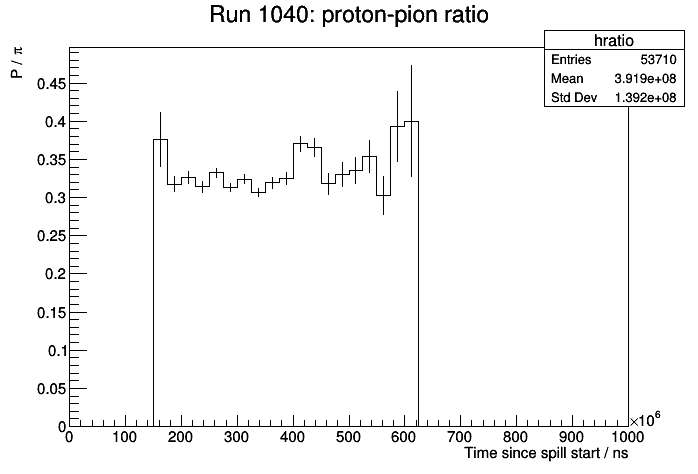
\includegraphics[width=\textwidth]{files/Figures/Run1040_proPiRatio}
%		\caption{The ratio of protons to pions as a function of time since the start of the beam spill. For these data, 1 moderator block was in place and the beam momentum was nominally 0.8~GeV/c. The data for this graph is from the sum of 255 spills.}
%		\label{fig:proPiRatio}
%	\end{minipage} 
%	\hspace{0.3cm}
%	\begin{minipage}[t]{0.48\textwidth}
%		\centering
%		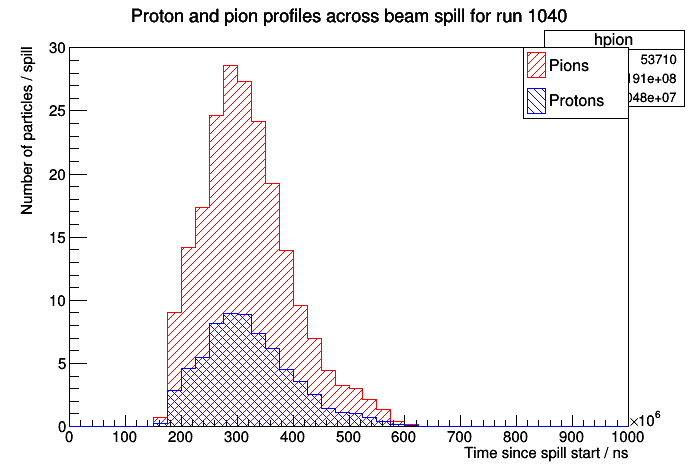
\includegraphics[width=\textwidth]{files/Figures/Run1040_proPiProf}
%		\caption{The number of protons and pions detected per spill by the DsToF as a function of time since the start of the beam spill. For these data, 1 moderator block was in place and the beam momentum was nominally 0.8~GeV/c. The data for this graph is from the sum of 255 spills.}
%		\label{fig:proPiProf}
%	\end{minipage}
%\end{figure}

Figure~\ref{fig:thetas4mip} shows the flux of particles identified as minimum ionizing particles across $\mathit{S4}$.
This flux is shown as as a function of the angle in the $x-y$ plane (see figure~\ref{fig:setup} for the definitions of these axes) for varying numbers of moderator blocks.
For all numbers of moderator blocks, the peak number of minimum ionizing particle events occurs at a value of $\theta$ between $1^{\circ}$ and $2^{\circ}$.
Similarly the number of proton events per spill, shown in figure~\ref{fig:thetas4pro} peaks at a value of $\theta$ of approximately $2^{\circ}$.

Two factors have an impact on the position of the peak:
the limited efficiency of $\mathit{S4}$ at the ends of the bars (near to either of the photomultiplier tubes) causes a smaller fraction of signal hits to be recorded in these regions. 
This limited efficiency is caused by the requirement that both PMTs record a waveform in order for a signal to be recorded.
This requirement is made, in order to reduce the number of false positives from dark noise in the PMT.
\todo[inline]{JOCELYN: Need a quantitative statement about the efficiency vs. angle here.}

The angular overlap of $\mathit{S2}$ and $\mathit{S4}$ also plays a role in the position of the peak. 
Figure~\ref{fig:angularDistS1} shows that, when observed from $\mathit{S1}$, a limited area of $\mathit{S4}$ is shadowed by the active area of $\mathit{S2}$.
\todo[inline]{JOCELYN: this explanation should go earlier in the dicsussion of the coordinate system for each ToF wall...}
Given the requirement that a signal must be observed in $\mathit{S2}$, it is clear that all of the events that are observed in $\mathit{S4}$ are from this region of overlap.

Figure~\ref{fig:thetas4mip} also indicates that initially, an increasing number of moderator blocks results in an increased total MIP flux through $\mathit{S4}$. 
However, upon the addition of the fourth moderator block the flux of MIPs appears to fall.
This is observed due to the off-axis position of both $\mathit{S2}$ and $\mathit{S4}$, avoiding many of the unmoderated beam particles striking these detectors.
Due to scattering processes in the moderator, a greater number of MIPs are incident upon $\mathit{S2}$ and $\mathit{S4}$, with more scattering occurring with greater numbers of moderator blocks.
%The drop off in the number of MIPs observed in the four block data is likely due to the overscattering of the protons and MIPs as stated previously.

When changing from an unmoderated beam to the configuration with 1 moderator block, the proton flux shown in Figure~\ref{fig:thetas4pro} initially sees an increase in the total number of events in $\mathit{S4}$.
However, upon the addition of further moderator blocks, the total number of protons observed in $\mathit{S4}$ falls.
The initial increase is similar to that for the MIP flux, with increased scattering causing more protons to pass through the off-axis $\mathit{S2}$ and $\mathit{S4}$.
The subsequent decrease is likely due to the larger loss of energy of the protons in the thicker moderator.
In turn, this leads to attenuation of protons in the TPC resulting in fewer observed events in $\mathit{S4}$.

\begin{figure}[!ht]
  \begin{minipage}[t]{0.48\textwidth}
    \begin{adjustbox}{max totalsize={\textwidth}{.35\textheight},center}
      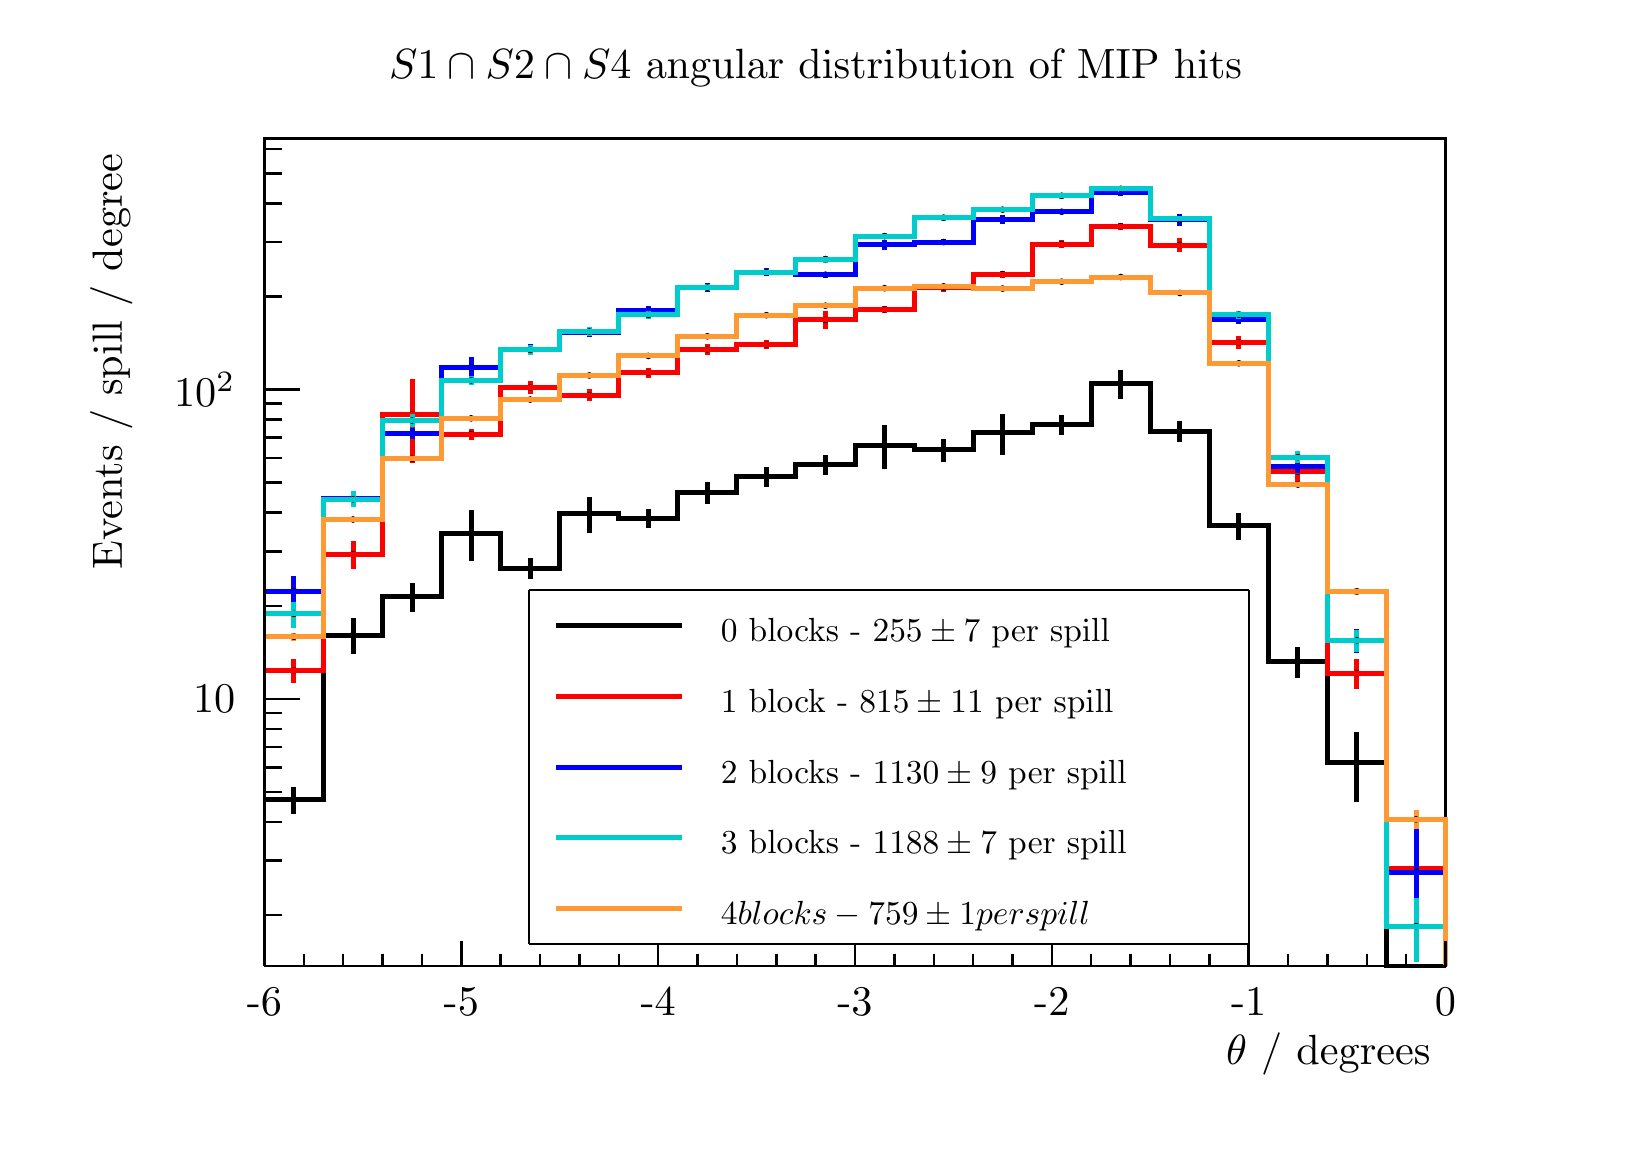
\begin{tikzpicture}
\pgfdeclareplotmark{cross} {
\pgfpathmoveto{\pgfpoint{-0.3\pgfplotmarksize}{\pgfplotmarksize}}
\pgfpathlineto{\pgfpoint{+0.3\pgfplotmarksize}{\pgfplotmarksize}}
\pgfpathlineto{\pgfpoint{+0.3\pgfplotmarksize}{0.3\pgfplotmarksize}}
\pgfpathlineto{\pgfpoint{+1\pgfplotmarksize}{0.3\pgfplotmarksize}}
\pgfpathlineto{\pgfpoint{+1\pgfplotmarksize}{-0.3\pgfplotmarksize}}
\pgfpathlineto{\pgfpoint{+0.3\pgfplotmarksize}{-0.3\pgfplotmarksize}}
\pgfpathlineto{\pgfpoint{+0.3\pgfplotmarksize}{-1.\pgfplotmarksize}}
\pgfpathlineto{\pgfpoint{-0.3\pgfplotmarksize}{-1.\pgfplotmarksize}}
\pgfpathlineto{\pgfpoint{-0.3\pgfplotmarksize}{-0.3\pgfplotmarksize}}
\pgfpathlineto{\pgfpoint{-1.\pgfplotmarksize}{-0.3\pgfplotmarksize}}
\pgfpathlineto{\pgfpoint{-1.\pgfplotmarksize}{0.3\pgfplotmarksize}}
\pgfpathlineto{\pgfpoint{-0.3\pgfplotmarksize}{0.3\pgfplotmarksize}}
\pgfpathclose
\pgfusepathqstroke
}
\pgfdeclareplotmark{cross*} {
\pgfpathmoveto{\pgfpoint{-0.3\pgfplotmarksize}{\pgfplotmarksize}}
\pgfpathlineto{\pgfpoint{+0.3\pgfplotmarksize}{\pgfplotmarksize}}
\pgfpathlineto{\pgfpoint{+0.3\pgfplotmarksize}{0.3\pgfplotmarksize}}
\pgfpathlineto{\pgfpoint{+1\pgfplotmarksize}{0.3\pgfplotmarksize}}
\pgfpathlineto{\pgfpoint{+1\pgfplotmarksize}{-0.3\pgfplotmarksize}}
\pgfpathlineto{\pgfpoint{+0.3\pgfplotmarksize}{-0.3\pgfplotmarksize}}
\pgfpathlineto{\pgfpoint{+0.3\pgfplotmarksize}{-1.\pgfplotmarksize}}
\pgfpathlineto{\pgfpoint{-0.3\pgfplotmarksize}{-1.\pgfplotmarksize}}
\pgfpathlineto{\pgfpoint{-0.3\pgfplotmarksize}{-0.3\pgfplotmarksize}}
\pgfpathlineto{\pgfpoint{-1.\pgfplotmarksize}{-0.3\pgfplotmarksize}}
\pgfpathlineto{\pgfpoint{-1.\pgfplotmarksize}{0.3\pgfplotmarksize}}
\pgfpathlineto{\pgfpoint{-0.3\pgfplotmarksize}{0.3\pgfplotmarksize}}
\pgfpathclose
\pgfusepathqfillstroke
}
\pgfdeclareplotmark{newstar} {
\pgfpathmoveto{\pgfqpoint{0pt}{\pgfplotmarksize}}
\pgfpathlineto{\pgfqpointpolar{44}{0.5\pgfplotmarksize}}
\pgfpathlineto{\pgfqpointpolar{18}{\pgfplotmarksize}}
\pgfpathlineto{\pgfqpointpolar{-20}{0.5\pgfplotmarksize}}
\pgfpathlineto{\pgfqpointpolar{-54}{\pgfplotmarksize}}
\pgfpathlineto{\pgfqpointpolar{-90}{0.5\pgfplotmarksize}}
\pgfpathlineto{\pgfqpointpolar{234}{\pgfplotmarksize}}
\pgfpathlineto{\pgfqpointpolar{198}{0.5\pgfplotmarksize}}
\pgfpathlineto{\pgfqpointpolar{162}{\pgfplotmarksize}}
\pgfpathlineto{\pgfqpointpolar{134}{0.5\pgfplotmarksize}}
\pgfpathclose
\pgfusepathqstroke
}
\pgfdeclareplotmark{newstar*} {
\pgfpathmoveto{\pgfqpoint{0pt}{\pgfplotmarksize}}
\pgfpathlineto{\pgfqpointpolar{44}{0.5\pgfplotmarksize}}
\pgfpathlineto{\pgfqpointpolar{18}{\pgfplotmarksize}}
\pgfpathlineto{\pgfqpointpolar{-20}{0.5\pgfplotmarksize}}
\pgfpathlineto{\pgfqpointpolar{-54}{\pgfplotmarksize}}
\pgfpathlineto{\pgfqpointpolar{-90}{0.5\pgfplotmarksize}}
\pgfpathlineto{\pgfqpointpolar{234}{\pgfplotmarksize}}
\pgfpathlineto{\pgfqpointpolar{198}{0.5\pgfplotmarksize}}
\pgfpathlineto{\pgfqpointpolar{162}{\pgfplotmarksize}}
\pgfpathlineto{\pgfqpointpolar{134}{0.5\pgfplotmarksize}}
\pgfpathclose
\pgfusepathqfillstroke
}
\definecolor{c}{rgb}{1,1,1};
\draw [color=c, fill=c] (0,0) rectangle (20,14.0115);
\draw [color=c, fill=c] (3,2.10172) rectangle (18,12.6103);
\definecolor{c}{rgb}{0,0,0};
\draw [c,line width=0.9] (3,2.10172) -- (3,12.6103) -- (18,12.6103) -- (18,2.10172) -- (3,2.10172);
\definecolor{c}{rgb}{1,1,1};
\draw [color=c, fill=c] (3,2.10172) rectangle (18,12.6103);
\definecolor{c}{rgb}{0,0,0};
\draw [c,line width=0.9] (3,2.10172) -- (3,12.6103) -- (18,12.6103) -- (18,2.10172) -- (3,2.10172);
\definecolor{c}{rgb}{0,0,0.6};
\draw [c,line width=0.9] (3,2.10172) -- (3.75,2.10172) -- (3.75,2.10172) -- (4.5,2.10172) -- (4.5,2.10172) -- (5.25,2.10172) -- (5.25,2.10172) -- (6,2.10172) -- (6,2.10172) -- (6.75,2.10172) -- (6.75,2.10172) -- (7.5,2.10172) -- (7.5,2.10172) --
 (8.25,2.10172) -- (8.25,2.10172) -- (9,2.10172) -- (9,2.10172) -- (9.75,2.10172) -- (9.75,2.10172) -- (10.5,2.10172) -- (10.5,2.10172) -- (11.25,2.10172) -- (11.25,2.10172) -- (12,2.10172) -- (12,2.10172) -- (12.75,2.10172) -- (12.75,2.10172) --
 (13.5,2.10172) -- (13.5,2.10172) -- (14.25,2.10172) -- (14.25,2.10172) -- (15,2.10172) -- (15,2.10172) -- (15.75,2.10172) -- (15.75,2.10172) -- (16.5,2.10172) -- (16.5,2.10172) -- (17.25,2.10172) -- (17.25,2.10172) -- (18,2.10172) -- (18,2.10172);
\definecolor{c}{rgb}{0,0,0};
\draw [c,line width=0.9] (3,2.10172) -- (18,2.10172);
\draw [c,line width=0.9] (3,2.41698) -- (3,2.10172);
\draw [c,line width=0.9] (3.5,2.25935) -- (3.5,2.10172);
\draw [c,line width=0.9] (4,2.25935) -- (4,2.10172);
\draw [c,line width=0.9] (4.5,2.25935) -- (4.5,2.10172);
\draw [c,line width=0.9] (5,2.25935) -- (5,2.10172);
\draw [c,line width=0.9] (5.5,2.41698) -- (5.5,2.10172);
\draw [c,line width=0.9] (6,2.25935) -- (6,2.10172);
\draw [c,line width=0.9] (6.5,2.25935) -- (6.5,2.10172);
\draw [c,line width=0.9] (7,2.25935) -- (7,2.10172);
\draw [c,line width=0.9] (7.5,2.25935) -- (7.5,2.10172);
\draw [c,line width=0.9] (8,2.41698) -- (8,2.10172);
\draw [c,line width=0.9] (8.5,2.25935) -- (8.5,2.10172);
\draw [c,line width=0.9] (9,2.25935) -- (9,2.10172);
\draw [c,line width=0.9] (9.5,2.25935) -- (9.5,2.10172);
\draw [c,line width=0.9] (10,2.25935) -- (10,2.10172);
\draw [c,line width=0.9] (10.5,2.41698) -- (10.5,2.10172);
\draw [c,line width=0.9] (11,2.25935) -- (11,2.10172);
\draw [c,line width=0.9] (11.5,2.25935) -- (11.5,2.10172);
\draw [c,line width=0.9] (12,2.25935) -- (12,2.10172);
\draw [c,line width=0.9] (12.5,2.25935) -- (12.5,2.10172);
\draw [c,line width=0.9] (13,2.41698) -- (13,2.10172);
\draw [c,line width=0.9] (13.5,2.25935) -- (13.5,2.10172);
\draw [c,line width=0.9] (14,2.25935) -- (14,2.10172);
\draw [c,line width=0.9] (14.5,2.25935) -- (14.5,2.10172);
\draw [c,line width=0.9] (15,2.25935) -- (15,2.10172);
\draw [c,line width=0.9] (15.5,2.41698) -- (15.5,2.10172);
\draw [c,line width=0.9] (16,2.25935) -- (16,2.10172);
\draw [c,line width=0.9] (16.5,2.25935) -- (16.5,2.10172);
\draw [c,line width=0.9] (17,2.25935) -- (17,2.10172);
\draw [c,line width=0.9] (17.5,2.25935) -- (17.5,2.10172);
\draw [c,line width=0.9] (18,2.41698) -- (18,2.10172);
\draw [anchor=base] (3,1.4712) node[scale=1.52731, color=c, rotate=0]{-6};
\draw [anchor=base] (5.5,1.4712) node[scale=1.52731, color=c, rotate=0]{-5};
\draw [anchor=base] (8,1.4712) node[scale=1.52731, color=c, rotate=0]{-4};
\draw [anchor=base] (10.5,1.4712) node[scale=1.52731, color=c, rotate=0]{-3};
\draw [anchor=base] (13,1.4712) node[scale=1.52731, color=c, rotate=0]{-2};
\draw [anchor=base] (15.5,1.4712) node[scale=1.52731, color=c, rotate=0]{-1};
\draw [anchor=base] (18,1.4712) node[scale=1.52731, color=c, rotate=0]{0};
\draw [anchor= east] (18,0.980802) node[scale=1.52731, color=c, rotate=0]{$\theta$ / degrees};
\draw [c,line width=0.9] (3,2.10172) -- (3,12.6103);
\draw [c,line width=0.9] (3.225,2.74878) -- (3,2.74878);
\draw [c,line width=0.9] (3.225,3.44048) -- (3,3.44048);
\draw [c,line width=0.9] (3.225,3.93125) -- (3,3.93125);
\draw [c,line width=0.9] (3.225,4.31191) -- (3,4.31191);
\draw [c,line width=0.9] (3.225,4.62294) -- (3,4.62294);
\draw [c,line width=0.9] (3.225,4.88591) -- (3,4.88591);
\draw [c,line width=0.9] (3.225,5.11371) -- (3,5.11371);
\draw [c,line width=0.9] (3.225,5.31464) -- (3,5.31464);
\draw [c,line width=0.9] (3.45,5.49438) -- (3,5.49438);
\draw [anchor= east] (2.82,5.49438) node[scale=1.52731, color=c, rotate=0]{10};
\draw [c,line width=0.9] (3.225,6.67684) -- (3,6.67684);
\draw [c,line width=0.9] (3.225,7.36854) -- (3,7.36854);
\draw [c,line width=0.9] (3.225,7.85931) -- (3,7.85931);
\draw [c,line width=0.9] (3.225,8.23998) -- (3,8.23998);
\draw [c,line width=0.9] (3.225,8.55101) -- (3,8.55101);
\draw [c,line width=0.9] (3.225,8.81398) -- (3,8.81398);
\draw [c,line width=0.9] (3.225,9.04177) -- (3,9.04177);
\draw [c,line width=0.9] (3.225,9.2427) -- (3,9.2427);
\draw [c,line width=0.9] (3.45,9.42244) -- (3,9.42244);
\draw [anchor= east] (2.82,9.42244) node[scale=1.52731, color=c, rotate=0]{$10^{2}$};
\draw [c,line width=0.9] (3.225,10.6049) -- (3,10.6049);
\draw [c,line width=0.9] (3.225,11.2966) -- (3,11.2966);
\draw [c,line width=0.9] (3.225,11.7874) -- (3,11.7874);
\draw [c,line width=0.9] (3.225,12.168) -- (3,12.168);
\draw [c,line width=0.9] (3.225,12.4791) -- (3,12.4791);
\draw [anchor= east] (1.05444,12.6103) node[scale=1.52731, color=c, rotate=90]{ Events / spill / degree};
\draw [c,line width=1.8] (3.375,4.03479) -- (3.375,4.21511);
\draw [c,line width=1.8] (3.375,4.21511) -- (3.375,4.37817);
\foreach \P in {(3.375,4.21511)}{\draw[mark options={color=c,fill=c},mark size=2.402402pt,mark=*,mark size=1pt] plot coordinates {\P};}
\draw [c,line width=1.8] (4.125,6.06456) -- (4.125,6.30527);
\draw [c,line width=1.8] (4.125,6.30527) -- (4.125,6.51617);
\foreach \P in {(4.125,6.30527)}{\draw[mark options={color=c,fill=c},mark size=2.402402pt,mark=*,mark size=1pt] plot coordinates {\P};}
\draw [c,line width=1.8] (4.875,6.59289) -- (4.875,6.79255);
\draw [c,line width=1.8] (4.875,6.79255) -- (4.875,6.97128);
\foreach \P in {(4.875,6.79255)}{\draw[mark options={color=c,fill=c},mark size=2.402402pt,mark=*,mark size=1pt] plot coordinates {\P};}
\draw [c,line width=1.8] (5.625,7.24345) -- (5.625,7.59827);
\draw [c,line width=1.8] (5.625,7.59827) -- (5.625,7.89184);
\foreach \P in {(5.625,7.59827)}{\draw[mark options={color=c,fill=c},mark size=2.402402pt,mark=*,mark size=1pt] plot coordinates {\P};}
\draw [c,line width=1.8] (6.375,7.0209) -- (6.375,7.15415);
\draw [c,line width=1.8] (6.375,7.15415) -- (6.375,7.27775);
\foreach \P in {(6.375,7.15415)}{\draw[mark options={color=c,fill=c},mark size=2.402402pt,mark=*,mark size=1pt] plot coordinates {\P};}
\draw [c,line width=1.8] (7.125,7.59869) -- (7.125,7.84484);
\draw [c,line width=1.8] (7.125,7.84484) -- (7.125,8.05991);
\foreach \P in {(7.125,7.84484)}{\draw[mark options={color=c,fill=c},mark size=2.402402pt,mark=*,mark size=1pt] plot coordinates {\P};}
\draw [c,line width=1.8] (7.875,7.66128) -- (7.875,7.78909);
\draw [c,line width=1.8] (7.875,7.78909) -- (7.875,7.90799);
\foreach \P in {(7.875,7.78909)}{\draw[mark options={color=c,fill=c},mark size=2.402402pt,mark=*,mark size=1pt] plot coordinates {\P};}
\draw [c,line width=1.8] (8.625,7.96983) -- (8.625,8.11244);
\draw [c,line width=1.8] (8.625,8.11244) -- (8.625,8.24405);
\foreach \P in {(8.625,8.11244)}{\draw[mark options={color=c,fill=c},mark size=2.402402pt,mark=*,mark size=1pt] plot coordinates {\P};}
\draw [c,line width=1.8] (9.375,8.17892) -- (9.375,8.31357);
\draw [c,line width=1.8] (9.375,8.31357) -- (9.375,8.43837);
\foreach \P in {(9.375,8.31357)}{\draw[mark options={color=c,fill=c},mark size=2.402402pt,mark=*,mark size=1pt] plot coordinates {\P};}
\draw [c,line width=1.8] (10.125,8.33421) -- (10.125,8.46593);
\draw [c,line width=1.8] (10.125,8.46593) -- (10.125,8.58821);
\foreach \P in {(10.125,8.46593)}{\draw[mark options={color=c,fill=c},mark size=2.402402pt,mark=*,mark size=1pt] plot coordinates {\P};}
\draw [c,line width=1.8] (10.875,8.40736) -- (10.875,8.71387);
\draw [c,line width=1.8] (10.875,8.71387) -- (10.875,8.9736);
\foreach \P in {(10.875,8.71387)}{\draw[mark options={color=c,fill=c},mark size=2.402402pt,mark=*,mark size=1pt] plot coordinates {\P};}
\draw [c,line width=1.8] (11.625,8.50247) -- (11.625,8.65545);
\draw [c,line width=1.8] (11.625,8.65545) -- (11.625,8.79583);
\foreach \P in {(11.625,8.65545)}{\draw[mark options={color=c,fill=c},mark size=2.402402pt,mark=*,mark size=1pt] plot coordinates {\P};}
\draw [c,line width=1.8] (12.375,8.59757) -- (12.375,8.87469);
\draw [c,line width=1.8] (12.375,8.87469) -- (12.375,9.11301);
\foreach \P in {(12.375,8.87469)}{\draw[mark options={color=c,fill=c},mark size=2.402402pt,mark=*,mark size=1pt] plot coordinates {\P};}
\draw [c,line width=1.8] (13.125,8.84578) -- (13.125,8.97996);
\draw [c,line width=1.8] (13.125,8.97996) -- (13.125,9.10434);
\foreach \P in {(13.125,8.97996)}{\draw[mark options={color=c,fill=c},mark size=2.402402pt,mark=*,mark size=1pt] plot coordinates {\P};}
\draw [c,line width=1.8] (13.875,9.30442) -- (13.875,9.49928);
\draw [c,line width=1.8] (13.875,9.49928) -- (13.875,9.67416);
\foreach \P in {(13.875,9.49928)}{\draw[mark options={color=c,fill=c},mark size=2.402402pt,mark=*,mark size=1pt] plot coordinates {\P};}
\draw [c,line width=1.8] (14.625,8.75179) -- (14.625,8.89211);
\draw [c,line width=1.8] (14.625,8.89211) -- (14.625,9.02176);
\foreach \P in {(14.625,8.89211)}{\draw[mark options={color=c,fill=c},mark size=2.402402pt,mark=*,mark size=1pt] plot coordinates {\P};}
\draw [c,line width=1.8] (15.375,7.50871) -- (15.375,7.69028);
\draw [c,line width=1.8] (15.375,7.69028) -- (15.375,7.85438);
\foreach \P in {(15.375,7.69028)}{\draw[mark options={color=c,fill=c},mark size=2.402402pt,mark=*,mark size=1pt] plot coordinates {\P};}
\draw [c,line width=1.8] (16.125,5.75699) -- (16.125,5.96327);
\draw [c,line width=1.8] (16.125,5.96327) -- (16.125,6.14727);
\foreach \P in {(16.125,5.96327)}{\draw[mark options={color=c,fill=c},mark size=2.402402pt,mark=*,mark size=1pt] plot coordinates {\P};}
\draw [c,line width=1.8] (16.875,4.1801) -- (16.875,4.6868);
\draw [c,line width=1.8] (16.875,4.6868) -- (16.875,5.07696);
\foreach \P in {(16.875,4.6868)}{\draw[mark options={color=c,fill=c},mark size=2.402402pt,mark=*,mark size=1pt] plot coordinates {\P};}
\draw [c,line width=1.8] (3,4.21511) -- (3.75,4.21511) -- (3.75,6.30527) -- (4.5,6.30527) -- (4.5,6.79255) -- (5.25,6.79255) -- (5.25,7.59827) -- (6,7.59827) -- (6,7.15415) -- (6.75,7.15415) -- (6.75,7.84484) -- (7.5,7.84484) -- (7.5,7.78909) --
 (8.25,7.78909) -- (8.25,8.11244) -- (9,8.11244) -- (9,8.31357) -- (9.75,8.31357) -- (9.75,8.46593) -- (10.5,8.46593) -- (10.5,8.71387) -- (11.25,8.71387) -- (11.25,8.65545) -- (12,8.65545) -- (12,8.87469) -- (12.75,8.87469) -- (12.75,8.97996) --
 (13.5,8.97996) -- (13.5,9.49928) -- (14.25,9.49928) -- (14.25,8.89211) -- (15,8.89211) -- (15,7.69028) -- (15.75,7.69028) -- (15.75,5.96327) -- (16.5,5.96327) -- (16.5,4.6868) -- (17.25,4.6868) -- (17.25,2.10172) -- (18,2.10172) -- (18,2.10172);
\definecolor{c}{rgb}{1,0,0};
\draw [c,line width=1.8] (3.375,5.69435) -- (3.375,5.85486);
\draw [c,line width=1.8] (3.375,5.85486) -- (3.375,6.00157);
\definecolor{c}{rgb}{0,0,0};
\foreach \P in {(3.375,5.85486)}{\draw[mark options={color=c,fill=c},mark size=2.402402pt,mark=*,mark size=1pt] plot coordinates {\P};}
\definecolor{c}{rgb}{1,0,0};
\draw [c,line width=1.8] (4.125,7.13733) -- (4.125,7.33122);
\draw [c,line width=1.8] (4.125,7.33122) -- (4.125,7.50531);
\definecolor{c}{rgb}{0,0,0};
\foreach \P in {(4.125,7.33122)}{\draw[mark options={color=c,fill=c},mark size=2.402402pt,mark=*,mark size=1pt] plot coordinates {\P};}
\definecolor{c}{rgb}{1,0,0};
\draw [c,line width=1.8] (4.875,8.49291) -- (4.875,9.10662);
\draw [c,line width=1.8] (4.875,9.10662) -- (4.875,9.55702);
\definecolor{c}{rgb}{0,0,0};
\foreach \P in {(4.875,9.10662)}{\draw[mark options={color=c,fill=c},mark size=2.402402pt,mark=*,mark size=1pt] plot coordinates {\P};}
\definecolor{c}{rgb}{1,0,0};
\draw [c,line width=1.8] (5.625,8.78671) -- (5.625,8.85696);
\draw [c,line width=1.8] (5.625,8.85696) -- (5.625,8.92444);
\definecolor{c}{rgb}{0,0,0};
\foreach \P in {(5.625,8.85696)}{\draw[mark options={color=c,fill=c},mark size=2.402402pt,mark=*,mark size=1pt] plot coordinates {\P};}
\definecolor{c}{rgb}{1,0,0};
\draw [c,line width=1.8] (6.375,9.36058) -- (6.375,9.44798);
\draw [c,line width=1.8] (6.375,9.44798) -- (6.375,9.53112);
\definecolor{c}{rgb}{0,0,0};
\foreach \P in {(6.375,9.44798)}{\draw[mark options={color=c,fill=c},mark size=2.402402pt,mark=*,mark size=1pt] plot coordinates {\P};}
\definecolor{c}{rgb}{1,0,0};
\draw [c,line width=1.8] (7.125,9.27103) -- (7.125,9.34886);
\draw [c,line width=1.8] (7.125,9.34886) -- (7.125,9.4233);
\definecolor{c}{rgb}{0,0,0};
\foreach \P in {(7.125,9.34886)}{\draw[mark options={color=c,fill=c},mark size=2.402402pt,mark=*,mark size=1pt] plot coordinates {\P};}
\definecolor{c}{rgb}{1,0,0};
\draw [c,line width=1.8] (7.875,9.57391) -- (7.875,9.6376);
\draw [c,line width=1.8] (7.875,9.6376) -- (7.875,9.69901);
\definecolor{c}{rgb}{0,0,0};
\foreach \P in {(7.875,9.6376)}{\draw[mark options={color=c,fill=c},mark size=2.402402pt,mark=*,mark size=1pt] plot coordinates {\P};}
\definecolor{c}{rgb}{1,0,0};
\draw [c,line width=1.8] (8.625,9.86531) -- (8.625,9.93131);
\draw [c,line width=1.8] (8.625,9.93131) -- (8.625,9.99484);
\definecolor{c}{rgb}{0,0,0};
\foreach \P in {(8.625,9.93131)}{\draw[mark options={color=c,fill=c},mark size=2.402402pt,mark=*,mark size=1pt] plot coordinates {\P};}
\definecolor{c}{rgb}{1,0,0};
\draw [c,line width=1.8] (9.375,9.93416) -- (9.375,9.99291);
\draw [c,line width=1.8] (9.375,9.99291) -- (9.375,10.0497);
\definecolor{c}{rgb}{0,0,0};
\foreach \P in {(9.375,9.99291)}{\draw[mark options={color=c,fill=c},mark size=2.402402pt,mark=*,mark size=1pt] plot coordinates {\P};}
\definecolor{c}{rgb}{1,0,0};
\draw [c,line width=1.8] (10.125,10.1876) -- (10.125,10.3081);
\draw [c,line width=1.8] (10.125,10.3081) -- (10.125,10.4207);
\definecolor{c}{rgb}{0,0,0};
\foreach \P in {(10.125,10.3081)}{\draw[mark options={color=c,fill=c},mark size=2.402402pt,mark=*,mark size=1pt] plot coordinates {\P};}
\definecolor{c}{rgb}{1,0,0};
\draw [c,line width=1.8] (10.875,10.3908) -- (10.875,10.4405);
\draw [c,line width=1.8] (10.875,10.4405) -- (10.875,10.4888);
\definecolor{c}{rgb}{0,0,0};
\foreach \P in {(10.875,10.4405)}{\draw[mark options={color=c,fill=c},mark size=2.402402pt,mark=*,mark size=1pt] plot coordinates {\P};}
\definecolor{c}{rgb}{1,0,0};
\draw [c,line width=1.8] (11.625,10.6611) -- (11.625,10.7143);
\draw [c,line width=1.8] (11.625,10.7143) -- (11.625,10.7659);
\definecolor{c}{rgb}{0,0,0};
\foreach \P in {(11.625,10.7143)}{\draw[mark options={color=c,fill=c},mark size=2.402402pt,mark=*,mark size=1pt] plot coordinates {\P};}
\definecolor{c}{rgb}{1,0,0};
\draw [c,line width=1.8] (12.375,10.842) -- (12.375,10.8886);
\draw [c,line width=1.8] (12.375,10.8886) -- (12.375,10.934);
\definecolor{c}{rgb}{0,0,0};
\foreach \P in {(12.375,10.8886)}{\draw[mark options={color=c,fill=c},mark size=2.402402pt,mark=*,mark size=1pt] plot coordinates {\P};}
\definecolor{c}{rgb}{1,0,0};
\draw [c,line width=1.8] (13.125,11.2205) -- (13.125,11.2707);
\draw [c,line width=1.8] (13.125,11.2707) -- (13.125,11.3196);
\definecolor{c}{rgb}{0,0,0};
\foreach \P in {(13.125,11.2707)}{\draw[mark options={color=c,fill=c},mark size=2.402402pt,mark=*,mark size=1pt] plot coordinates {\P};}
\definecolor{c}{rgb}{1,0,0};
\draw [c,line width=1.8] (13.875,11.4485) -- (13.875,11.4966);
\draw [c,line width=1.8] (13.875,11.4966) -- (13.875,11.5434);
\definecolor{c}{rgb}{0,0,0};
\foreach \P in {(13.875,11.4966)}{\draw[mark options={color=c,fill=c},mark size=2.402402pt,mark=*,mark size=1pt] plot coordinates {\P};}
\definecolor{c}{rgb}{1,0,0};
\draw [c,line width=1.8] (14.625,11.1707) -- (14.625,11.258);
\draw [c,line width=1.8] (14.625,11.258) -- (14.625,11.3411);
\definecolor{c}{rgb}{0,0,0};
\foreach \P in {(14.625,11.258)}{\draw[mark options={color=c,fill=c},mark size=2.402402pt,mark=*,mark size=1pt] plot coordinates {\P};}
\definecolor{c}{rgb}{1,0,0};
\draw [c,line width=1.8] (15.375,9.94073) -- (15.375,10.0212);
\draw [c,line width=1.8] (15.375,10.0212) -- (15.375,10.098);
\definecolor{c}{rgb}{0,0,0};
\foreach \P in {(15.375,10.0212)}{\draw[mark options={color=c,fill=c},mark size=2.402402pt,mark=*,mark size=1pt] plot coordinates {\P};}
\definecolor{c}{rgb}{1,0,0};
\draw [c,line width=1.8] (16.125,8.20348) -- (16.125,8.37878);
\draw [c,line width=1.8] (16.125,8.37878) -- (16.125,8.53773);
\definecolor{c}{rgb}{0,0,0};
\foreach \P in {(16.125,8.37878)}{\draw[mark options={color=c,fill=c},mark size=2.402402pt,mark=*,mark size=1pt] plot coordinates {\P};}
\definecolor{c}{rgb}{1,0,0};
\draw [c,line width=1.8] (16.875,5.61778) -- (16.875,5.81947);
\draw [c,line width=1.8] (16.875,5.81947) -- (16.875,5.99982);
\definecolor{c}{rgb}{0,0,0};
\foreach \P in {(16.875,5.81947)}{\draw[mark options={color=c,fill=c},mark size=2.402402pt,mark=*,mark size=1pt] plot coordinates {\P};}
\definecolor{c}{rgb}{1,0,0};
\draw [c,line width=1.8] (17.625,2.81258) -- (17.625,3.33608);
\draw [c,line width=1.8] (17.625,3.33608) -- (17.625,3.7361);
\definecolor{c}{rgb}{0,0,0};
\foreach \P in {(17.625,3.33608)}{\draw[mark options={color=c,fill=c},mark size=2.402402pt,mark=*,mark size=1pt] plot coordinates {\P};}
\definecolor{c}{rgb}{1,0,0};
\draw [c,line width=1.8] (3,5.85486) -- (3.75,5.85486) -- (3.75,7.33122) -- (4.5,7.33122) -- (4.5,9.10662) -- (5.25,9.10662) -- (5.25,8.85696) -- (6,8.85696) -- (6,9.44798) -- (6.75,9.44798) -- (6.75,9.34886) -- (7.5,9.34886) -- (7.5,9.6376) --
 (8.25,9.6376) -- (8.25,9.93131) -- (9,9.93131) -- (9,9.99291) -- (9.75,9.99291) -- (9.75,10.3081) -- (10.5,10.3081) -- (10.5,10.4405) -- (11.25,10.4405) -- (11.25,10.7143) -- (12,10.7143) -- (12,10.8886) -- (12.75,10.8886) -- (12.75,11.2707) --
 (13.5,11.2707) -- (13.5,11.4966) -- (14.25,11.4966) -- (14.25,11.258) -- (15,11.258) -- (15,10.0212) -- (15.75,10.0212) -- (15.75,8.37878) -- (16.5,8.37878) -- (16.5,5.81947) -- (17.25,5.81947) -- (17.25,3.33608) -- (18,3.33608) -- (18,2.10172);
\definecolor{c}{rgb}{0,0,1};
\draw [c,line width=1.8] (3.375,6.65616) -- (3.375,6.8638);
\draw [c,line width=1.8] (3.375,6.8638) -- (3.375,7.04889);
\definecolor{c}{rgb}{0,0,0};
\foreach \P in {(3.375,6.8638)}{\draw[mark options={color=c,fill=c},mark size=2.402402pt,mark=*,mark size=1pt] plot coordinates {\P};}
\definecolor{c}{rgb}{0,0,1};
\draw [c,line width=1.8] (4.125,7.95275) -- (4.125,8.03964);
\draw [c,line width=1.8] (4.125,8.03964) -- (4.125,8.12233);
\definecolor{c}{rgb}{0,0,0};
\foreach \P in {(4.125,8.03964)}{\draw[mark options={color=c,fill=c},mark size=2.402402pt,mark=*,mark size=1pt] plot coordinates {\P};}
\definecolor{c}{rgb}{0,0,1};
\draw [c,line width=1.8] (4.875,8.79676) -- (4.875,8.86516);
\draw [c,line width=1.8] (4.875,8.86516) -- (4.875,8.93093);
\definecolor{c}{rgb}{0,0,0};
\foreach \P in {(4.875,8.86516)}{\draw[mark options={color=c,fill=c},mark size=2.402402pt,mark=*,mark size=1pt] plot coordinates {\P};}
\definecolor{c}{rgb}{0,0,1};
\draw [c,line width=1.8] (5.625,9.56311) -- (5.625,9.70472);
\draw [c,line width=1.8] (5.625,9.70472) -- (5.625,9.83546);
\definecolor{c}{rgb}{0,0,0};
\foreach \P in {(5.625,9.70472)}{\draw[mark options={color=c,fill=c},mark size=2.402402pt,mark=*,mark size=1pt] plot coordinates {\P};}
\definecolor{c}{rgb}{0,0,1};
\draw [c,line width=1.8] (6.375,9.86868) -- (6.375,9.93349);
\draw [c,line width=1.8] (6.375,9.93349) -- (6.375,9.99594);
\definecolor{c}{rgb}{0,0,0};
\foreach \P in {(6.375,9.93349)}{\draw[mark options={color=c,fill=c},mark size=2.402402pt,mark=*,mark size=1pt] plot coordinates {\P};}
\definecolor{c}{rgb}{0,0,1};
\draw [c,line width=1.8] (7.125,10.0923) -- (7.125,10.1467);
\draw [c,line width=1.8] (7.125,10.1467) -- (7.125,10.1994);
\definecolor{c}{rgb}{0,0,0};
\foreach \P in {(7.125,10.1467)}{\draw[mark options={color=c,fill=c},mark size=2.402402pt,mark=*,mark size=1pt] plot coordinates {\P};}
\definecolor{c}{rgb}{0,0,1};
\draw [c,line width=1.8] (7.875,10.3723) -- (7.875,10.4285);
\draw [c,line width=1.8] (7.875,10.4285) -- (7.875,10.483);
\definecolor{c}{rgb}{0,0,0};
\foreach \P in {(7.875,10.4285)}{\draw[mark options={color=c,fill=c},mark size=2.402402pt,mark=*,mark size=1pt] plot coordinates {\P};}
\definecolor{c}{rgb}{0,0,1};
\draw [c,line width=1.8] (8.625,10.6569) -- (8.625,10.7171);
\draw [c,line width=1.8] (8.625,10.7171) -- (8.625,10.7754);
\definecolor{c}{rgb}{0,0,0};
\foreach \P in {(8.625,10.7171)}{\draw[mark options={color=c,fill=c},mark size=2.402402pt,mark=*,mark size=1pt] plot coordinates {\P};}
\definecolor{c}{rgb}{0,0,1};
\draw [c,line width=1.8] (9.375,10.8604) -- (9.375,10.9138);
\draw [c,line width=1.8] (9.375,10.9138) -- (9.375,10.9655);
\definecolor{c}{rgb}{0,0,0};
\foreach \P in {(9.375,10.9138)}{\draw[mark options={color=c,fill=c},mark size=2.402402pt,mark=*,mark size=1pt] plot coordinates {\P};}
\definecolor{c}{rgb}{0,0,1};
\draw [c,line width=1.8] (10.125,10.8426) -- (10.125,10.8814);
\draw [c,line width=1.8] (10.125,10.8814) -- (10.125,10.9193);
\definecolor{c}{rgb}{0,0,0};
\foreach \P in {(10.125,10.8814)}{\draw[mark options={color=c,fill=c},mark size=2.402402pt,mark=*,mark size=1pt] plot coordinates {\P};}
\definecolor{c}{rgb}{0,0,1};
\draw [c,line width=1.8] (10.875,11.197) -- (10.875,11.2635);
\draw [c,line width=1.8] (10.875,11.2635) -- (10.875,11.3274);
\definecolor{c}{rgb}{0,0,0};
\foreach \P in {(10.875,11.2635)}{\draw[mark options={color=c,fill=c},mark size=2.402402pt,mark=*,mark size=1pt] plot coordinates {\P};}
\definecolor{c}{rgb}{0,0,1};
\draw [c,line width=1.8] (11.625,11.2611) -- (11.625,11.2957);
\draw [c,line width=1.8] (11.625,11.2957) -- (11.625,11.3296);
\definecolor{c}{rgb}{0,0,0};
\foreach \P in {(11.625,11.2957)}{\draw[mark options={color=c,fill=c},mark size=2.402402pt,mark=*,mark size=1pt] plot coordinates {\P};}
\definecolor{c}{rgb}{0,0,1};
\draw [c,line width=1.8] (12.375,11.5281) -- (12.375,11.5817);
\draw [c,line width=1.8] (12.375,11.5817) -- (12.375,11.6336);
\definecolor{c}{rgb}{0,0,0};
\foreach \P in {(12.375,11.5817)}{\draw[mark options={color=c,fill=c},mark size=2.402402pt,mark=*,mark size=1pt] plot coordinates {\P};}
\definecolor{c}{rgb}{0,0,1};
\draw [c,line width=1.8] (13.125,11.65) -- (13.125,11.6807);
\draw [c,line width=1.8] (13.125,11.6807) -- (13.125,11.7108);
\definecolor{c}{rgb}{0,0,0};
\foreach \P in {(13.125,11.6807)}{\draw[mark options={color=c,fill=c},mark size=2.402402pt,mark=*,mark size=1pt] plot coordinates {\P};}
\definecolor{c}{rgb}{0,0,1};
\draw [c,line width=1.8] (13.875,11.8858) -- (13.875,11.9233);
\draw [c,line width=1.8] (13.875,11.9233) -- (13.875,11.96);
\definecolor{c}{rgb}{0,0,0};
\foreach \P in {(13.875,11.9233)}{\draw[mark options={color=c,fill=c},mark size=2.402402pt,mark=*,mark size=1pt] plot coordinates {\P};}
\definecolor{c}{rgb}{0,0,1};
\draw [c,line width=1.8] (14.625,11.5052) -- (14.625,11.5773);
\draw [c,line width=1.8] (14.625,11.5773) -- (14.625,11.6465);
\definecolor{c}{rgb}{0,0,0};
\foreach \P in {(14.625,11.5773)}{\draw[mark options={color=c,fill=c},mark size=2.402402pt,mark=*,mark size=1pt] plot coordinates {\P};}
\definecolor{c}{rgb}{0,0,1};
\draw [c,line width=1.8] (15.375,10.2584) -- (15.375,10.3138);
\draw [c,line width=1.8] (15.375,10.3138) -- (15.375,10.3674);
\definecolor{c}{rgb}{0,0,0};
\foreach \P in {(15.375,10.3138)}{\draw[mark options={color=c,fill=c},mark size=2.402402pt,mark=*,mark size=1pt] plot coordinates {\P};}
\definecolor{c}{rgb}{0,0,1};
\draw [c,line width=1.8] (16.125,8.36025) -- (16.125,8.4466);
\draw [c,line width=1.8] (16.125,8.4466) -- (16.125,8.52878);
\definecolor{c}{rgb}{0,0,0};
\foreach \P in {(16.125,8.4466)}{\draw[mark options={color=c,fill=c},mark size=2.402402pt,mark=*,mark size=1pt] plot coordinates {\P};}
\definecolor{c}{rgb}{0,0,1};
\draw [c,line width=1.8] (16.875,6.08301) -- (16.875,6.24076);
\draw [c,line width=1.8] (16.875,6.24076) -- (16.875,6.38515);
\definecolor{c}{rgb}{0,0,0};
\foreach \P in {(16.875,6.24076)}{\draw[mark options={color=c,fill=c},mark size=2.402402pt,mark=*,mark size=1pt] plot coordinates {\P};}
\definecolor{c}{rgb}{0,0,1};
\draw [c,line width=1.8] (17.625,2.24304) -- (17.625,3.29519);
\draw [c,line width=1.8] (17.625,3.29519) -- (17.625,3.94114);
\definecolor{c}{rgb}{0,0,0};
\foreach \P in {(17.625,3.29519)}{\draw[mark options={color=c,fill=c},mark size=2.402402pt,mark=*,mark size=1pt] plot coordinates {\P};}
\definecolor{c}{rgb}{0,0,1};
\draw [c,line width=1.8] (3,6.8638) -- (3.75,6.8638) -- (3.75,8.03964) -- (4.5,8.03964) -- (4.5,8.86516) -- (5.25,8.86516) -- (5.25,9.70472) -- (6,9.70472) -- (6,9.93349) -- (6.75,9.93349) -- (6.75,10.1467) -- (7.5,10.1467) -- (7.5,10.4285) --
 (8.25,10.4285) -- (8.25,10.7171) -- (9,10.7171) -- (9,10.9138) -- (9.75,10.9138) -- (9.75,10.8814) -- (10.5,10.8814) -- (10.5,11.2635) -- (11.25,11.2635) -- (11.25,11.2957) -- (12,11.2957) -- (12,11.5817) -- (12.75,11.5817) -- (12.75,11.6807) --
 (13.5,11.6807) -- (13.5,11.9233) -- (14.25,11.9233) -- (14.25,11.5773) -- (15,11.5773) -- (15,10.3138) -- (15.75,10.3138) -- (15.75,8.4466) -- (16.5,8.4466) -- (16.5,6.24076) -- (17.25,6.24076) -- (17.25,3.29519) -- (18,3.29519) -- (18,2.10172);
\definecolor{c}{rgb}{0,0.8,0.8};
\draw [c,line width=1.8] (3.375,6.40051) -- (3.375,6.57328);
\draw [c,line width=1.8] (3.375,6.57328) -- (3.375,6.73014);
\definecolor{c}{rgb}{0,0,0};
\foreach \P in {(3.375,6.57328)}{\draw[mark options={color=c,fill=c},mark size=2.402402pt,mark=*,mark size=1pt] plot coordinates {\P};}
\definecolor{c}{rgb}{0,0.8,0.8};
\draw [c,line width=1.8] (4.125,7.9248) -- (4.125,8.02937);
\draw [c,line width=1.8] (4.125,8.02937) -- (4.125,8.12789);
\definecolor{c}{rgb}{0,0,0};
\foreach \P in {(4.125,8.02937)}{\draw[mark options={color=c,fill=c},mark size=2.402402pt,mark=*,mark size=1pt] plot coordinates {\P};}
\definecolor{c}{rgb}{0,0.8,0.8};
\draw [c,line width=1.8] (4.875,8.94752) -- (4.875,9.02906);
\draw [c,line width=1.8] (4.875,9.02906) -- (4.875,9.10688);
\definecolor{c}{rgb}{0,0,0};
\foreach \P in {(4.875,9.02906)}{\draw[mark options={color=c,fill=c},mark size=2.402402pt,mark=*,mark size=1pt] plot coordinates {\P};}
\definecolor{c}{rgb}{0,0.8,0.8};
\draw [c,line width=1.8] (5.625,9.4765) -- (5.625,9.53891);
\draw [c,line width=1.8] (5.625,9.53891) -- (5.625,9.59913);
\definecolor{c}{rgb}{0,0,0};
\foreach \P in {(5.625,9.53891)}{\draw[mark options={color=c,fill=c},mark size=2.402402pt,mark=*,mark size=1pt] plot coordinates {\P};}
\definecolor{c}{rgb}{0,0.8,0.8};
\draw [c,line width=1.8] (6.375,9.86024) -- (6.375,9.92617);
\draw [c,line width=1.8] (6.375,9.92617) -- (6.375,9.98965);
\definecolor{c}{rgb}{0,0,0};
\foreach \P in {(6.375,9.92617)}{\draw[mark options={color=c,fill=c},mark size=2.402402pt,mark=*,mark size=1pt] plot coordinates {\P};}
\definecolor{c}{rgb}{0,0.8,0.8};
\draw [c,line width=1.8] (7.125,10.1072) -- (7.125,10.1601);
\draw [c,line width=1.8] (7.125,10.1601) -- (7.125,10.2114);
\definecolor{c}{rgb}{0,0,0};
\foreach \P in {(7.125,10.1601)}{\draw[mark options={color=c,fill=c},mark size=2.402402pt,mark=*,mark size=1pt] plot coordinates {\P};}
\definecolor{c}{rgb}{0,0.8,0.8};
\draw [c,line width=1.8] (7.875,10.3237) -- (7.875,10.3698);
\draw [c,line width=1.8] (7.875,10.3698) -- (7.875,10.4147);
\definecolor{c}{rgb}{0,0,0};
\foreach \P in {(7.875,10.3698)}{\draw[mark options={color=c,fill=c},mark size=2.402402pt,mark=*,mark size=1pt] plot coordinates {\P};}
\definecolor{c}{rgb}{0,0.8,0.8};
\draw [c,line width=1.8] (8.625,10.6703) -- (8.625,10.7158);
\draw [c,line width=1.8] (8.625,10.7158) -- (8.625,10.7602);
\definecolor{c}{rgb}{0,0,0};
\foreach \P in {(8.625,10.7158)}{\draw[mark options={color=c,fill=c},mark size=2.402402pt,mark=*,mark size=1pt] plot coordinates {\P};}
\definecolor{c}{rgb}{0,0.8,0.8};
\draw [c,line width=1.8] (9.375,10.8724) -- (9.375,10.9138);
\draw [c,line width=1.8] (9.375,10.9138) -- (9.375,10.9541);
\definecolor{c}{rgb}{0,0,0};
\foreach \P in {(9.375,10.9138)}{\draw[mark options={color=c,fill=c},mark size=2.402402pt,mark=*,mark size=1pt] plot coordinates {\P};}
\definecolor{c}{rgb}{0,0.8,0.8};
\draw [c,line width=1.8] (10.125,11.0354) -- (10.125,11.0796);
\draw [c,line width=1.8] (10.125,11.0796) -- (10.125,11.1227);
\definecolor{c}{rgb}{0,0,0};
\foreach \P in {(10.125,11.0796)}{\draw[mark options={color=c,fill=c},mark size=2.402402pt,mark=*,mark size=1pt] plot coordinates {\P};}
\definecolor{c}{rgb}{0,0.8,0.8};
\draw [c,line width=1.8] (10.875,11.3299) -- (10.875,11.3702);
\draw [c,line width=1.8] (10.875,11.3702) -- (10.875,11.4096);
\definecolor{c}{rgb}{0,0,0};
\foreach \P in {(10.875,11.3702)}{\draw[mark options={color=c,fill=c},mark size=2.402402pt,mark=*,mark size=1pt] plot coordinates {\P};}
\definecolor{c}{rgb}{0,0.8,0.8};
\draw [c,line width=1.8] (11.625,11.5661) -- (11.625,11.6059);
\draw [c,line width=1.8] (11.625,11.6059) -- (11.625,11.6448);
\definecolor{c}{rgb}{0,0,0};
\foreach \P in {(11.625,11.6059)}{\draw[mark options={color=c,fill=c},mark size=2.402402pt,mark=*,mark size=1pt] plot coordinates {\P};}
\definecolor{c}{rgb}{0,0.8,0.8};
\draw [c,line width=1.8] (12.375,11.672) -- (12.375,11.7071);
\draw [c,line width=1.8] (12.375,11.7071) -- (12.375,11.7414);
\definecolor{c}{rgb}{0,0,0};
\foreach \P in {(12.375,11.7071)}{\draw[mark options={color=c,fill=c},mark size=2.402402pt,mark=*,mark size=1pt] plot coordinates {\P};}
\definecolor{c}{rgb}{0,0.8,0.8};
\draw [c,line width=1.8] (13.125,11.8446) -- (13.125,11.8841);
\draw [c,line width=1.8] (13.125,11.8841) -- (13.125,11.9227);
\definecolor{c}{rgb}{0,0,0};
\foreach \P in {(13.125,11.8841)}{\draw[mark options={color=c,fill=c},mark size=2.402402pt,mark=*,mark size=1pt] plot coordinates {\P};}
\definecolor{c}{rgb}{0,0.8,0.8};
\draw [c,line width=1.8] (13.875,11.9367) -- (13.875,11.9724);
\draw [c,line width=1.8] (13.875,11.9724) -- (13.875,12.0075);
\definecolor{c}{rgb}{0,0,0};
\foreach \P in {(13.875,11.9724)}{\draw[mark options={color=c,fill=c},mark size=2.402402pt,mark=*,mark size=1pt] plot coordinates {\P};}
\definecolor{c}{rgb}{0,0.8,0.8};
\draw [c,line width=1.8] (14.625,11.5591) -- (14.625,11.5942);
\draw [c,line width=1.8] (14.625,11.5942) -- (14.625,11.6286);
\definecolor{c}{rgb}{0,0,0};
\foreach \P in {(14.625,11.5942)}{\draw[mark options={color=c,fill=c},mark size=2.402402pt,mark=*,mark size=1pt] plot coordinates {\P};}
\definecolor{c}{rgb}{0,0.8,0.8};
\draw [c,line width=1.8] (15.375,10.323) -- (15.375,10.3723);
\draw [c,line width=1.8] (15.375,10.3723) -- (15.375,10.4201);
\definecolor{c}{rgb}{0,0,0};
\foreach \P in {(15.375,10.3723)}{\draw[mark options={color=c,fill=c},mark size=2.402402pt,mark=*,mark size=1pt] plot coordinates {\P};}
\definecolor{c}{rgb}{0,0.8,0.8};
\draw [c,line width=1.8] (16.125,8.4846) -- (16.125,8.56423);
\draw [c,line width=1.8] (16.125,8.56423) -- (16.125,8.64031);
\definecolor{c}{rgb}{0,0,0};
\foreach \P in {(16.125,8.56423)}{\draw[mark options={color=c,fill=c},mark size=2.402402pt,mark=*,mark size=1pt] plot coordinates {\P};}
\definecolor{c}{rgb}{0,0.8,0.8};
\draw [c,line width=1.8] (16.875,6.09143) -- (16.875,6.23765);
\draw [c,line width=1.8] (16.875,6.23765) -- (16.875,6.37232);
\definecolor{c}{rgb}{0,0,0};
\foreach \P in {(16.875,6.23765)}{\draw[mark options={color=c,fill=c},mark size=2.402402pt,mark=*,mark size=1pt] plot coordinates {\P};}
\definecolor{c}{rgb}{0,0.8,0.8};
\draw [c,line width=1.8] (17.625,2.14644) -- (17.625,2.60808);
\draw [c,line width=1.8] (17.625,2.60808) -- (17.625,2.97102);
\definecolor{c}{rgb}{0,0,0};
\foreach \P in {(17.625,2.60808)}{\draw[mark options={color=c,fill=c},mark size=2.402402pt,mark=*,mark size=1pt] plot coordinates {\P};}
\definecolor{c}{rgb}{0,0.8,0.8};
\draw [c,line width=1.8] (3,6.57328) -- (3.75,6.57328) -- (3.75,8.02937) -- (4.5,8.02937) -- (4.5,9.02906) -- (5.25,9.02906) -- (5.25,9.53891) -- (6,9.53891) -- (6,9.92617) -- (6.75,9.92617) -- (6.75,10.1601) -- (7.5,10.1601) -- (7.5,10.3698) --
 (8.25,10.3698) -- (8.25,10.7158) -- (9,10.7158) -- (9,10.9138) -- (9.75,10.9138) -- (9.75,11.0796) -- (10.5,11.0796) -- (10.5,11.3702) -- (11.25,11.3702) -- (11.25,11.6059) -- (12,11.6059) -- (12,11.7071) -- (12.75,11.7071) -- (12.75,11.8841) --
 (13.5,11.8841) -- (13.5,11.9724) -- (14.25,11.9724) -- (14.25,11.5942) -- (15,11.5942) -- (15,10.3723) -- (15.75,10.3723) -- (15.75,8.56423) -- (16.5,8.56423) -- (16.5,6.23765) -- (17.25,6.23765) -- (17.25,2.60808) -- (18,2.60808) -- (18,2.10172);
\definecolor{c}{rgb}{1,0.6,0.2};
\draw [c,line width=1.8] (3.375,6.23023) -- (3.375,6.28262);
\draw [c,line width=1.8] (3.375,6.28262) -- (3.375,6.33344);
\definecolor{c}{rgb}{0,0,0};
\foreach \P in {(3.375,6.28262)}{\draw[mark options={color=c,fill=c},mark size=2.402402pt,mark=*,mark size=1pt] plot coordinates {\P};}
\definecolor{c}{rgb}{1,0.6,0.2};
\draw [c,line width=1.8] (4.125,7.74046) -- (4.125,7.7725);
\draw [c,line width=1.8] (4.125,7.7725) -- (4.125,7.80395);
\definecolor{c}{rgb}{0,0,0};
\foreach \P in {(4.125,7.7725)}{\draw[mark options={color=c,fill=c},mark size=2.402402pt,mark=*,mark size=1pt] plot coordinates {\P};}
\definecolor{c}{rgb}{1,0.6,0.2};
\draw [c,line width=1.8] (4.875,8.51788) -- (4.875,8.54274);
\draw [c,line width=1.8] (4.875,8.54274) -- (4.875,8.56725);
\definecolor{c}{rgb}{0,0,0};
\foreach \P in {(4.875,8.54274)}{\draw[mark options={color=c,fill=c},mark size=2.402402pt,mark=*,mark size=1pt] plot coordinates {\P};}
\definecolor{c}{rgb}{1,0.6,0.2};
\draw [c,line width=1.8] (5.625,9.03253) -- (5.625,9.05691);
\draw [c,line width=1.8] (5.625,9.05691) -- (5.625,9.08095);
\definecolor{c}{rgb}{0,0,0};
\foreach \P in {(5.625,9.05691)}{\draw[mark options={color=c,fill=c},mark size=2.402402pt,mark=*,mark size=1pt] plot coordinates {\P};}
\definecolor{c}{rgb}{1,0.6,0.2};
\draw [c,line width=1.8] (6.375,9.27332) -- (6.375,9.29555);
\draw [c,line width=1.8] (6.375,9.29555) -- (6.375,9.31749);
\definecolor{c}{rgb}{0,0,0};
\foreach \P in {(6.375,9.29555)}{\draw[mark options={color=c,fill=c},mark size=2.402402pt,mark=*,mark size=1pt] plot coordinates {\P};}
\definecolor{c}{rgb}{1,0.6,0.2};
\draw [c,line width=1.8] (7.125,9.58119) -- (7.125,9.60165);
\draw [c,line width=1.8] (7.125,9.60165) -- (7.125,9.62187);
\definecolor{c}{rgb}{0,0,0};
\foreach \P in {(7.125,9.60165)}{\draw[mark options={color=c,fill=c},mark size=2.402402pt,mark=*,mark size=1pt] plot coordinates {\P};}
\definecolor{c}{rgb}{1,0.6,0.2};
\draw [c,line width=1.8] (7.875,9.83215) -- (7.875,9.84977);
\draw [c,line width=1.8] (7.875,9.84977) -- (7.875,9.86721);
\definecolor{c}{rgb}{0,0,0};
\foreach \P in {(7.875,9.84977)}{\draw[mark options={color=c,fill=c},mark size=2.402402pt,mark=*,mark size=1pt] plot coordinates {\P};}
\definecolor{c}{rgb}{1,0.6,0.2};
\draw [c,line width=1.8] (8.625,10.0829) -- (8.625,10.0985);
\draw [c,line width=1.8] (8.625,10.0985) -- (8.625,10.1139);
\definecolor{c}{rgb}{0,0,0};
\foreach \P in {(8.625,10.0985)}{\draw[mark options={color=c,fill=c},mark size=2.402402pt,mark=*,mark size=1pt] plot coordinates {\P};}
\definecolor{c}{rgb}{1,0.6,0.2};
\draw [c,line width=1.8] (9.375,10.3517) -- (9.375,10.367);
\draw [c,line width=1.8] (9.375,10.367) -- (9.375,10.3822);
\definecolor{c}{rgb}{0,0,0};
\foreach \P in {(9.375,10.367)}{\draw[mark options={color=c,fill=c},mark size=2.402402pt,mark=*,mark size=1pt] plot coordinates {\P};}
\definecolor{c}{rgb}{1,0.6,0.2};
\draw [c,line width=1.8] (10.125,10.4726) -- (10.125,10.4875);
\draw [c,line width=1.8] (10.125,10.4875) -- (10.125,10.5023);
\definecolor{c}{rgb}{0,0,0};
\foreach \P in {(10.125,10.4875)}{\draw[mark options={color=c,fill=c},mark size=2.402402pt,mark=*,mark size=1pt] plot coordinates {\P};}
\definecolor{c}{rgb}{1,0.6,0.2};
\draw [c,line width=1.8] (10.875,10.6961) -- (10.875,10.7097);
\draw [c,line width=1.8] (10.875,10.7097) -- (10.875,10.7231);
\definecolor{c}{rgb}{0,0,0};
\foreach \P in {(10.875,10.7097)}{\draw[mark options={color=c,fill=c},mark size=2.402402pt,mark=*,mark size=1pt] plot coordinates {\P};}
\definecolor{c}{rgb}{1,0.6,0.2};
\draw [c,line width=1.8] (11.625,10.7203) -- (11.625,10.7331);
\draw [c,line width=1.8] (11.625,10.7331) -- (11.625,10.7458);
\definecolor{c}{rgb}{0,0,0};
\foreach \P in {(11.625,10.7331)}{\draw[mark options={color=c,fill=c},mark size=2.402402pt,mark=*,mark size=1pt] plot coordinates {\P};}
\definecolor{c}{rgb}{1,0.6,0.2};
\draw [c,line width=1.8] (12.375,10.6913) -- (12.375,10.7048);
\draw [c,line width=1.8] (12.375,10.7048) -- (12.375,10.7181);
\definecolor{c}{rgb}{0,0,0};
\foreach \P in {(12.375,10.7048)}{\draw[mark options={color=c,fill=c},mark size=2.402402pt,mark=*,mark size=1pt] plot coordinates {\P};}
\definecolor{c}{rgb}{1,0.6,0.2};
\draw [c,line width=1.8] (13.125,10.7784) -- (13.125,10.792);
\draw [c,line width=1.8] (13.125,10.792) -- (13.125,10.8055);
\definecolor{c}{rgb}{0,0,0};
\foreach \P in {(13.125,10.792)}{\draw[mark options={color=c,fill=c},mark size=2.402402pt,mark=*,mark size=1pt] plot coordinates {\P};}
\definecolor{c}{rgb}{1,0.6,0.2};
\draw [c,line width=1.8] (13.875,10.8386) -- (13.875,10.8514);
\draw [c,line width=1.8] (13.875,10.8514) -- (13.875,10.8641);
\definecolor{c}{rgb}{0,0,0};
\foreach \P in {(13.875,10.8514)}{\draw[mark options={color=c,fill=c},mark size=2.402402pt,mark=*,mark size=1pt] plot coordinates {\P};}
\definecolor{c}{rgb}{1,0.6,0.2};
\draw [c,line width=1.8] (14.625,10.6349) -- (14.625,10.6491);
\draw [c,line width=1.8] (14.625,10.6491) -- (14.625,10.6632);
\definecolor{c}{rgb}{0,0,0};
\foreach \P in {(14.625,10.6491)}{\draw[mark options={color=c,fill=c},mark size=2.402402pt,mark=*,mark size=1pt] plot coordinates {\P};}
\definecolor{c}{rgb}{1,0.6,0.2};
\draw [c,line width=1.8] (15.375,9.73812) -- (15.375,9.75611);
\draw [c,line width=1.8] (15.375,9.75611) -- (15.375,9.77392);
\definecolor{c}{rgb}{0,0,0};
\foreach \P in {(15.375,9.75611)}{\draw[mark options={color=c,fill=c},mark size=2.402402pt,mark=*,mark size=1pt] plot coordinates {\P};}
\definecolor{c}{rgb}{1,0.6,0.2};
\draw [c,line width=1.8] (16.125,8.18706) -- (16.125,8.21553);
\draw [c,line width=1.8] (16.125,8.21553) -- (16.125,8.24354);
\definecolor{c}{rgb}{0,0,0};
\foreach \P in {(16.125,8.21553)}{\draw[mark options={color=c,fill=c},mark size=2.402402pt,mark=*,mark size=1pt] plot coordinates {\P};}
\definecolor{c}{rgb}{1,0.6,0.2};
\draw [c,line width=1.8] (16.875,6.81928) -- (16.875,6.85881);
\draw [c,line width=1.8] (16.875,6.85881) -- (16.875,6.89745);
\definecolor{c}{rgb}{0,0,0};
\foreach \P in {(16.875,6.85881)}{\draw[mark options={color=c,fill=c},mark size=2.402402pt,mark=*,mark size=1pt] plot coordinates {\P};}
\definecolor{c}{rgb}{1,0.6,0.2};
\draw [c,line width=1.8] (17.625,3.83824) -- (17.625,3.96394);
\draw [c,line width=1.8] (17.625,3.96394) -- (17.625,4.08102);
\definecolor{c}{rgb}{0,0,0};
\foreach \P in {(17.625,3.96394)}{\draw[mark options={color=c,fill=c},mark size=2.402402pt,mark=*,mark size=1pt] plot coordinates {\P};}
\definecolor{c}{rgb}{1,0.6,0.2};
\draw [c,line width=1.8] (3,6.28262) -- (3.75,6.28262) -- (3.75,7.7725) -- (4.5,7.7725) -- (4.5,8.54274) -- (5.25,8.54274) -- (5.25,9.05691) -- (6,9.05691) -- (6,9.29555) -- (6.75,9.29555) -- (6.75,9.60165) -- (7.5,9.60165) -- (7.5,9.84977) --
 (8.25,9.84977) -- (8.25,10.0985) -- (9,10.0985) -- (9,10.367) -- (9.75,10.367) -- (9.75,10.4875) -- (10.5,10.4875) -- (10.5,10.7097) -- (11.25,10.7097) -- (11.25,10.7331) -- (12,10.7331) -- (12,10.7048) -- (12.75,10.7048) -- (12.75,10.792) --
 (13.5,10.792) -- (13.5,10.8514) -- (14.25,10.8514) -- (14.25,10.6491) -- (15,10.6491) -- (15,9.75611) -- (15.75,9.75611) -- (15.75,8.21553) -- (16.5,8.21553) -- (16.5,6.85881) -- (17.25,6.85881) -- (17.25,3.96394) -- (18,3.96394) -- (18,2.10172);
\definecolor{c}{rgb}{0,0,0};
\draw [c,line width=0.9] (3,2.10172) -- (18,2.10172);
\draw [c,line width=0.9] (3,2.41698) -- (3,2.10172);
\draw [c,line width=0.9] (3.5,2.25935) -- (3.5,2.10172);
\draw [c,line width=0.9] (4,2.25935) -- (4,2.10172);
\draw [c,line width=0.9] (4.5,2.25935) -- (4.5,2.10172);
\draw [c,line width=0.9] (5,2.25935) -- (5,2.10172);
\draw [c,line width=0.9] (5.5,2.41698) -- (5.5,2.10172);
\draw [c,line width=0.9] (6,2.25935) -- (6,2.10172);
\draw [c,line width=0.9] (6.5,2.25935) -- (6.5,2.10172);
\draw [c,line width=0.9] (7,2.25935) -- (7,2.10172);
\draw [c,line width=0.9] (7.5,2.25935) -- (7.5,2.10172);
\draw [c,line width=0.9] (8,2.41698) -- (8,2.10172);
\draw [c,line width=0.9] (8.5,2.25935) -- (8.5,2.10172);
\draw [c,line width=0.9] (9,2.25935) -- (9,2.10172);
\draw [c,line width=0.9] (9.5,2.25935) -- (9.5,2.10172);
\draw [c,line width=0.9] (10,2.25935) -- (10,2.10172);
\draw [c,line width=0.9] (10.5,2.41698) -- (10.5,2.10172);
\draw [c,line width=0.9] (11,2.25935) -- (11,2.10172);
\draw [c,line width=0.9] (11.5,2.25935) -- (11.5,2.10172);
\draw [c,line width=0.9] (12,2.25935) -- (12,2.10172);
\draw [c,line width=0.9] (12.5,2.25935) -- (12.5,2.10172);
\draw [c,line width=0.9] (13,2.41698) -- (13,2.10172);
\draw [c,line width=0.9] (13.5,2.25935) -- (13.5,2.10172);
\draw [c,line width=0.9] (14,2.25935) -- (14,2.10172);
\draw [c,line width=0.9] (14.5,2.25935) -- (14.5,2.10172);
\draw [c,line width=0.9] (15,2.25935) -- (15,2.10172);
\draw [c,line width=0.9] (15.5,2.41698) -- (15.5,2.10172);
\draw [c,line width=0.9] (16,2.25935) -- (16,2.10172);
\draw [c,line width=0.9] (16.5,2.25935) -- (16.5,2.10172);
\draw [c,line width=0.9] (17,2.25935) -- (17,2.10172);
\draw [c,line width=0.9] (17.5,2.25935) -- (17.5,2.10172);
\draw [c,line width=0.9] (18,2.41698) -- (18,2.10172);
\draw [c,line width=0.9] (3,2.10172) -- (3,12.6103);
\draw [c,line width=0.9] (3.225,2.74878) -- (3,2.74878);
\draw [c,line width=0.9] (3.225,3.44048) -- (3,3.44048);
\draw [c,line width=0.9] (3.225,3.93125) -- (3,3.93125);
\draw [c,line width=0.9] (3.225,4.31191) -- (3,4.31191);
\draw [c,line width=0.9] (3.225,4.62294) -- (3,4.62294);
\draw [c,line width=0.9] (3.225,4.88591) -- (3,4.88591);
\draw [c,line width=0.9] (3.225,5.11371) -- (3,5.11371);
\draw [c,line width=0.9] (3.225,5.31464) -- (3,5.31464);
\draw [c,line width=0.9] (3.45,5.49438) -- (3,5.49438);
\draw [c,line width=0.9] (3.225,6.67684) -- (3,6.67684);
\draw [c,line width=0.9] (3.225,7.36854) -- (3,7.36854);
\draw [c,line width=0.9] (3.225,7.85931) -- (3,7.85931);
\draw [c,line width=0.9] (3.225,8.23998) -- (3,8.23998);
\draw [c,line width=0.9] (3.225,8.55101) -- (3,8.55101);
\draw [c,line width=0.9] (3.225,8.81398) -- (3,8.81398);
\draw [c,line width=0.9] (3.225,9.04177) -- (3,9.04177);
\draw [c,line width=0.9] (3.225,9.2427) -- (3,9.2427);
\draw [c,line width=0.9] (3.45,9.42244) -- (3,9.42244);
\draw [c,line width=0.9] (3.225,10.6049) -- (3,10.6049);
\draw [c,line width=0.9] (3.225,11.2966) -- (3,11.2966);
\draw [c,line width=0.9] (3.225,11.7874) -- (3,11.7874);
\draw [c,line width=0.9] (3.225,12.168) -- (3,12.168);
\draw [c,line width=0.9] (3.225,12.4791) -- (3,12.4791);
\draw (10,13.5116) node[scale=1.52731, color=c, rotate=0]{$S1 \cap S2 \cap S4$ angular distribution of MIP hits};
\definecolor{c}{rgb}{1,1,1};
\draw [color=c, fill=c] (6.36103,2.37822) rectangle (15.5014,6.87679);
\definecolor{c}{rgb}{0,0,0};
\draw [c,line width=0.9] (6.36103,2.37822) -- (15.5014,2.37822);
\draw [c,line width=0.9] (15.5014,2.37822) -- (15.5014,6.87679);
\draw [c,line width=0.9] (15.5014,6.87679) -- (6.36103,6.87679);
\draw [c,line width=0.9] (6.36103,6.87679) -- (6.36103,2.37822);
\draw [anchor=base west] (8.64613,6.2245) node[scale=1.20912, color=c, rotate=0]{0 blocks - $255 \pm 7$ per spill};
\draw [c,line width=1.8] (6.7038,6.42693) -- (8.30337,6.42693);
\draw [anchor=base west] (8.64613,5.32479) node[scale=1.20912, color=c, rotate=0]{1 block - $815 \pm 11$ per spill};
\definecolor{c}{rgb}{1,0,0};
\draw [c,line width=1.8] (6.7038,5.52722) -- (8.30337,5.52722);
\definecolor{c}{rgb}{0,0,0};
\draw [anchor=base west] (8.64613,4.42507) node[scale=1.20912, color=c, rotate=0]{2 blocks - $1130 \pm 9$ per spill};
\definecolor{c}{rgb}{0,0,1};
\draw [c,line width=1.8] (6.7038,4.62751) -- (8.30337,4.62751);
\definecolor{c}{rgb}{0,0,0};
\draw [anchor=base west] (8.64613,3.52536) node[scale=1.20912, color=c, rotate=0]{3 blocks - $1188 \pm 7$ per spill};
\definecolor{c}{rgb}{0,0.8,0.8};
\draw [c,line width=1.8] (6.7038,3.72779) -- (8.30337,3.72779);
\definecolor{c}{rgb}{0,0,0};
\draw [anchor=base west] (8.64613,2.62564) node[scale=1.20912, color=c, rotate=0]{$4 blocks - 759 \pm 1 per spill$};
\definecolor{c}{rgb}{1,0.6,0.2};
\draw [c,line width=1.8] (6.7038,2.82808) -- (8.30337,2.82808);
\end{tikzpicture}

    \end{adjustbox}
    \caption{Distribution of hits identified in $\mathit{S4}$ as minimum ionizing particles as a function of the number of moderator blocks and the horizontal off-axis angle, as measured from $\mathit{S1}$.}
    \label{fig:thetas4mip}
  \end{minipage}
  \hspace{0.3cm}
  \begin{minipage}[t]{0.48\textwidth}
    \begin{adjustbox}{max totalsize={\textwidth}{.35\textheight},center}
      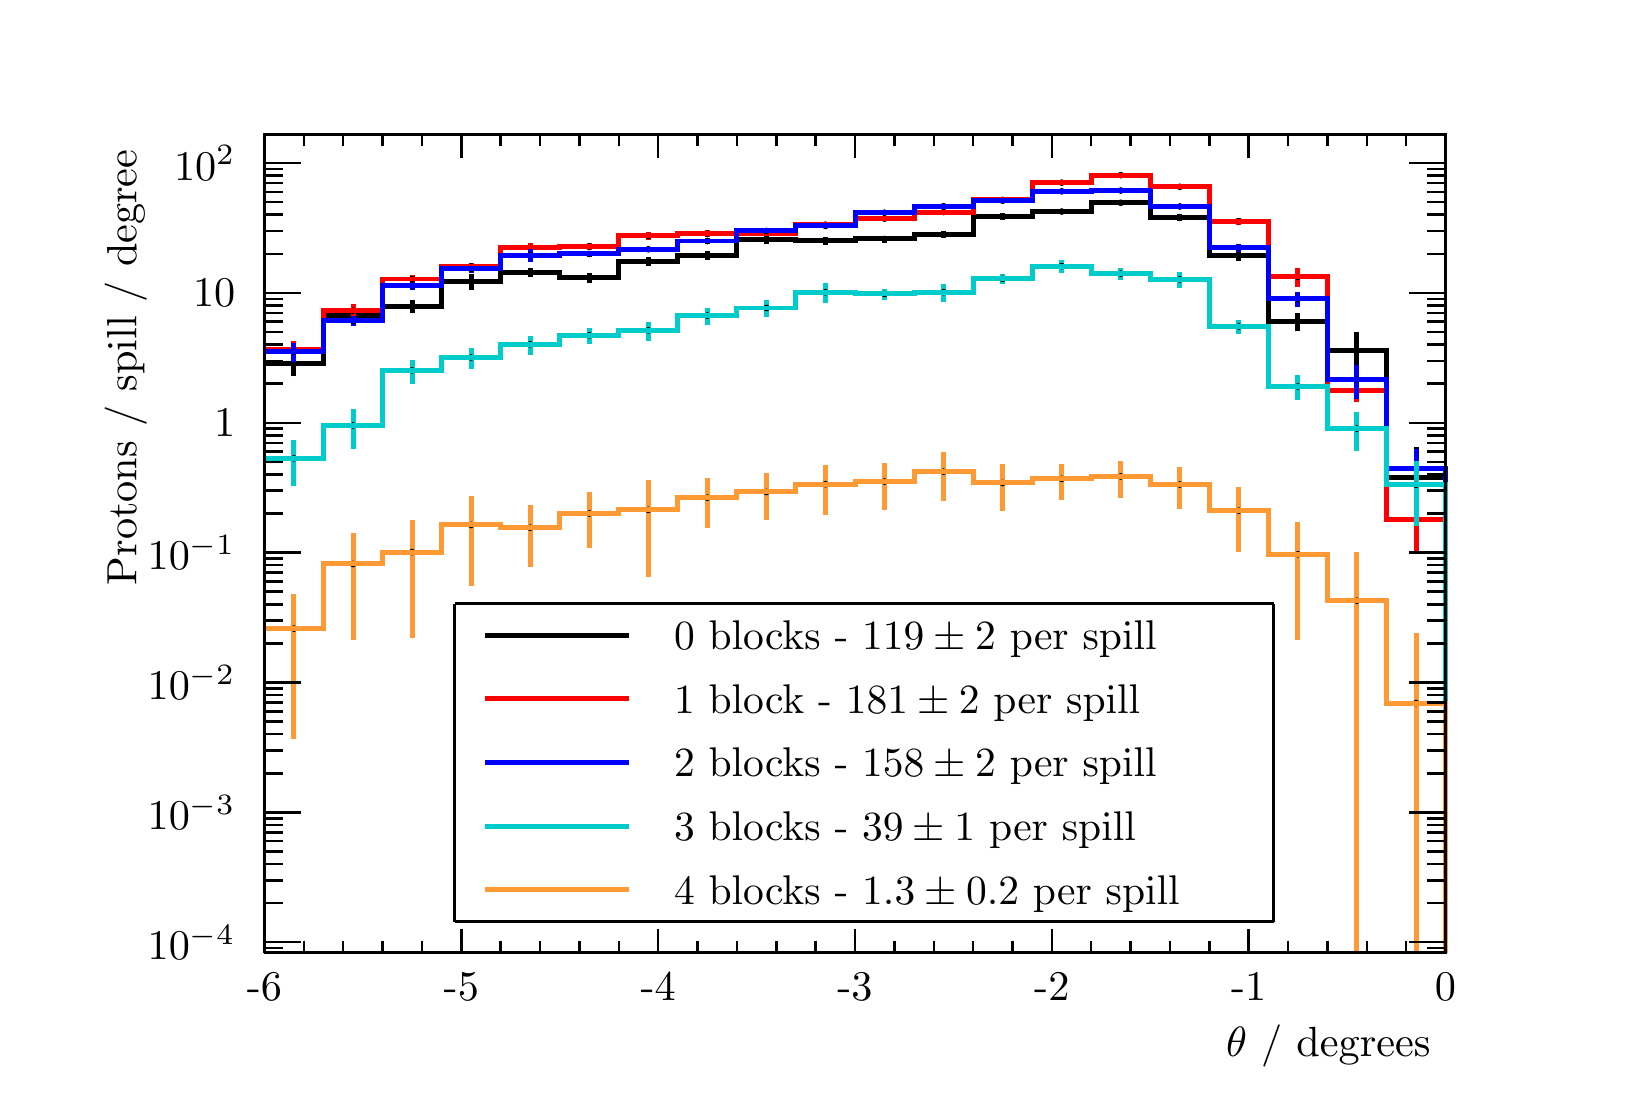
\begin{tikzpicture}
\pgfdeclareplotmark{cross} {
\pgfpathmoveto{\pgfpoint{-0.3\pgfplotmarksize}{\pgfplotmarksize}}
\pgfpathlineto{\pgfpoint{+0.3\pgfplotmarksize}{\pgfplotmarksize}}
\pgfpathlineto{\pgfpoint{+0.3\pgfplotmarksize}{0.3\pgfplotmarksize}}
\pgfpathlineto{\pgfpoint{+1\pgfplotmarksize}{0.3\pgfplotmarksize}}
\pgfpathlineto{\pgfpoint{+1\pgfplotmarksize}{-0.3\pgfplotmarksize}}
\pgfpathlineto{\pgfpoint{+0.3\pgfplotmarksize}{-0.3\pgfplotmarksize}}
\pgfpathlineto{\pgfpoint{+0.3\pgfplotmarksize}{-1.\pgfplotmarksize}}
\pgfpathlineto{\pgfpoint{-0.3\pgfplotmarksize}{-1.\pgfplotmarksize}}
\pgfpathlineto{\pgfpoint{-0.3\pgfplotmarksize}{-0.3\pgfplotmarksize}}
\pgfpathlineto{\pgfpoint{-1.\pgfplotmarksize}{-0.3\pgfplotmarksize}}
\pgfpathlineto{\pgfpoint{-1.\pgfplotmarksize}{0.3\pgfplotmarksize}}
\pgfpathlineto{\pgfpoint{-0.3\pgfplotmarksize}{0.3\pgfplotmarksize}}
\pgfpathclose
\pgfusepathqstroke
}
\pgfdeclareplotmark{cross*} {
\pgfpathmoveto{\pgfpoint{-0.3\pgfplotmarksize}{\pgfplotmarksize}}
\pgfpathlineto{\pgfpoint{+0.3\pgfplotmarksize}{\pgfplotmarksize}}
\pgfpathlineto{\pgfpoint{+0.3\pgfplotmarksize}{0.3\pgfplotmarksize}}
\pgfpathlineto{\pgfpoint{+1\pgfplotmarksize}{0.3\pgfplotmarksize}}
\pgfpathlineto{\pgfpoint{+1\pgfplotmarksize}{-0.3\pgfplotmarksize}}
\pgfpathlineto{\pgfpoint{+0.3\pgfplotmarksize}{-0.3\pgfplotmarksize}}
\pgfpathlineto{\pgfpoint{+0.3\pgfplotmarksize}{-1.\pgfplotmarksize}}
\pgfpathlineto{\pgfpoint{-0.3\pgfplotmarksize}{-1.\pgfplotmarksize}}
\pgfpathlineto{\pgfpoint{-0.3\pgfplotmarksize}{-0.3\pgfplotmarksize}}
\pgfpathlineto{\pgfpoint{-1.\pgfplotmarksize}{-0.3\pgfplotmarksize}}
\pgfpathlineto{\pgfpoint{-1.\pgfplotmarksize}{0.3\pgfplotmarksize}}
\pgfpathlineto{\pgfpoint{-0.3\pgfplotmarksize}{0.3\pgfplotmarksize}}
\pgfpathclose
\pgfusepathqfillstroke
}
\pgfdeclareplotmark{newstar} {
\pgfpathmoveto{\pgfqpoint{0pt}{\pgfplotmarksize}}
\pgfpathlineto{\pgfqpointpolar{44}{0.5\pgfplotmarksize}}
\pgfpathlineto{\pgfqpointpolar{18}{\pgfplotmarksize}}
\pgfpathlineto{\pgfqpointpolar{-20}{0.5\pgfplotmarksize}}
\pgfpathlineto{\pgfqpointpolar{-54}{\pgfplotmarksize}}
\pgfpathlineto{\pgfqpointpolar{-90}{0.5\pgfplotmarksize}}
\pgfpathlineto{\pgfqpointpolar{234}{\pgfplotmarksize}}
\pgfpathlineto{\pgfqpointpolar{198}{0.5\pgfplotmarksize}}
\pgfpathlineto{\pgfqpointpolar{162}{\pgfplotmarksize}}
\pgfpathlineto{\pgfqpointpolar{134}{0.5\pgfplotmarksize}}
\pgfpathclose
\pgfusepathqstroke
}
\pgfdeclareplotmark{newstar*} {
\pgfpathmoveto{\pgfqpoint{0pt}{\pgfplotmarksize}}
\pgfpathlineto{\pgfqpointpolar{44}{0.5\pgfplotmarksize}}
\pgfpathlineto{\pgfqpointpolar{18}{\pgfplotmarksize}}
\pgfpathlineto{\pgfqpointpolar{-20}{0.5\pgfplotmarksize}}
\pgfpathlineto{\pgfqpointpolar{-54}{\pgfplotmarksize}}
\pgfpathlineto{\pgfqpointpolar{-90}{0.5\pgfplotmarksize}}
\pgfpathlineto{\pgfqpointpolar{234}{\pgfplotmarksize}}
\pgfpathlineto{\pgfqpointpolar{198}{0.5\pgfplotmarksize}}
\pgfpathlineto{\pgfqpointpolar{162}{\pgfplotmarksize}}
\pgfpathlineto{\pgfqpointpolar{134}{0.5\pgfplotmarksize}}
\pgfpathclose
\pgfusepathqfillstroke
}
\definecolor{c}{rgb}{1,1,1};
\draw [color=c, fill=c] (0,0) rectangle (20,13.4957);
\draw [color=c, fill=c] (3,1.75444) rectangle (18,12.1461);
\definecolor{c}{rgb}{0,0,0};
\draw [c,line width=0.9] (3,1.75444) -- (3,12.1461) -- (18,12.1461) -- (18,1.75444) -- (3,1.75444);
\definecolor{c}{rgb}{1,1,1};
\draw [color=c, fill=c] (3,1.75444) rectangle (18,12.1461);
\definecolor{c}{rgb}{0,0,0};
\draw [c,line width=0.9] (3,1.75444) -- (3,12.1461) -- (18,12.1461) -- (18,1.75444) -- (3,1.75444);
\draw [c,line width=0.9] (3,1.75444) -- (3.75,1.75444) -- (3.75,1.75444) -- (4.5,1.75444) -- (4.5,1.75444) -- (5.25,1.75444) -- (5.25,1.75444) -- (6,1.75444) -- (6,1.75444) -- (6.75,1.75444) -- (6.75,1.75444) -- (7.5,1.75444) -- (7.5,1.75444) --
 (8.25,1.75444) -- (8.25,1.75444) -- (9,1.75444) -- (9,1.75444) -- (9.75,1.75444) -- (9.75,1.75444) -- (10.5,1.75444) -- (10.5,1.75444) -- (11.25,1.75444) -- (11.25,1.75444) -- (12,1.75444) -- (12,1.75444) -- (12.75,1.75444) -- (12.75,1.75444) --
 (13.5,1.75444) -- (13.5,1.75444) -- (14.25,1.75444) -- (14.25,1.75444) -- (15,1.75444) -- (15,1.75444) -- (15.75,1.75444) -- (15.75,1.75444) -- (16.5,1.75444) -- (16.5,1.75444) -- (17.25,1.75444) -- (17.25,1.75444) -- (18,1.75444) -- (18,1.75444);
\draw [c,line width=0.9] (3,1.75444) -- (18,1.75444);
\draw [c,line width=0.9] (3,2.05809) -- (3,1.75444);
\draw [c,line width=0.9] (3.5,1.90627) -- (3.5,1.75444);
\draw [c,line width=0.9] (4,1.90627) -- (4,1.75444);
\draw [c,line width=0.9] (4.5,1.90627) -- (4.5,1.75444);
\draw [c,line width=0.9] (5,1.90627) -- (5,1.75444);
\draw [c,line width=0.9] (5.5,2.05809) -- (5.5,1.75444);
\draw [c,line width=0.9] (6,1.90627) -- (6,1.75444);
\draw [c,line width=0.9] (6.5,1.90627) -- (6.5,1.75444);
\draw [c,line width=0.9] (7,1.90627) -- (7,1.75444);
\draw [c,line width=0.9] (7.5,1.90627) -- (7.5,1.75444);
\draw [c,line width=0.9] (8,2.05809) -- (8,1.75444);
\draw [c,line width=0.9] (8.5,1.90627) -- (8.5,1.75444);
\draw [c,line width=0.9] (9,1.90627) -- (9,1.75444);
\draw [c,line width=0.9] (9.5,1.90627) -- (9.5,1.75444);
\draw [c,line width=0.9] (10,1.90627) -- (10,1.75444);
\draw [c,line width=0.9] (10.5,2.05809) -- (10.5,1.75444);
\draw [c,line width=0.9] (11,1.90627) -- (11,1.75444);
\draw [c,line width=0.9] (11.5,1.90627) -- (11.5,1.75444);
\draw [c,line width=0.9] (12,1.90627) -- (12,1.75444);
\draw [c,line width=0.9] (12.5,1.90627) -- (12.5,1.75444);
\draw [c,line width=0.9] (13,2.05809) -- (13,1.75444);
\draw [c,line width=0.9] (13.5,1.90627) -- (13.5,1.75444);
\draw [c,line width=0.9] (14,1.90627) -- (14,1.75444);
\draw [c,line width=0.9] (14.5,1.90627) -- (14.5,1.75444);
\draw [c,line width=0.9] (15,1.90627) -- (15,1.75444);
\draw [c,line width=0.9] (15.5,2.05809) -- (15.5,1.75444);
\draw [c,line width=0.9] (16,1.90627) -- (16,1.75444);
\draw [c,line width=0.9] (16.5,1.90627) -- (16.5,1.75444);
\draw [c,line width=0.9] (17,1.90627) -- (17,1.75444);
\draw [c,line width=0.9] (17.5,1.90627) -- (17.5,1.75444);
\draw [c,line width=0.9] (18,2.05809) -- (18,1.75444);
\draw [anchor=base] (3,1.14713) node[scale=1.52731, color=c, rotate=0]{-6};
\draw [anchor=base] (5.5,1.14713) node[scale=1.52731, color=c, rotate=0]{-5};
\draw [anchor=base] (8,1.14713) node[scale=1.52731, color=c, rotate=0]{-4};
\draw [anchor=base] (10.5,1.14713) node[scale=1.52731, color=c, rotate=0]{-3};
\draw [anchor=base] (13,1.14713) node[scale=1.52731, color=c, rotate=0]{-2};
\draw [anchor=base] (15.5,1.14713) node[scale=1.52731, color=c, rotate=0]{-1};
\draw [anchor=base] (18,1.14713) node[scale=1.52731, color=c, rotate=0]{0};
\draw [anchor= east] (18,0.566819) node[scale=1.52731, color=c, rotate=0]{$ \theta$ / degrees};
\draw [c,line width=0.9] (3,12.1461) -- (18,12.1461);
\draw [c,line width=0.9] (3,11.8425) -- (3,12.1461);
\draw [c,line width=0.9] (3.5,11.9943) -- (3.5,12.1461);
\draw [c,line width=0.9] (4,11.9943) -- (4,12.1461);
\draw [c,line width=0.9] (4.5,11.9943) -- (4.5,12.1461);
\draw [c,line width=0.9] (5,11.9943) -- (5,12.1461);
\draw [c,line width=0.9] (5.5,11.8425) -- (5.5,12.1461);
\draw [c,line width=0.9] (6,11.9943) -- (6,12.1461);
\draw [c,line width=0.9] (6.5,11.9943) -- (6.5,12.1461);
\draw [c,line width=0.9] (7,11.9943) -- (7,12.1461);
\draw [c,line width=0.9] (7.5,11.9943) -- (7.5,12.1461);
\draw [c,line width=0.9] (8,11.8425) -- (8,12.1461);
\draw [c,line width=0.9] (8.5,11.9943) -- (8.5,12.1461);
\draw [c,line width=0.9] (9,11.9943) -- (9,12.1461);
\draw [c,line width=0.9] (9.5,11.9943) -- (9.5,12.1461);
\draw [c,line width=0.9] (10,11.9943) -- (10,12.1461);
\draw [c,line width=0.9] (10.5,11.8425) -- (10.5,12.1461);
\draw [c,line width=0.9] (11,11.9943) -- (11,12.1461);
\draw [c,line width=0.9] (11.5,11.9943) -- (11.5,12.1461);
\draw [c,line width=0.9] (12,11.9943) -- (12,12.1461);
\draw [c,line width=0.9] (12.5,11.9943) -- (12.5,12.1461);
\draw [c,line width=0.9] (13,11.8425) -- (13,12.1461);
\draw [c,line width=0.9] (13.5,11.9943) -- (13.5,12.1461);
\draw [c,line width=0.9] (14,11.9943) -- (14,12.1461);
\draw [c,line width=0.9] (14.5,11.9943) -- (14.5,12.1461);
\draw [c,line width=0.9] (15,11.9943) -- (15,12.1461);
\draw [c,line width=0.9] (15.5,11.8425) -- (15.5,12.1461);
\draw [c,line width=0.9] (16,11.9943) -- (16,12.1461);
\draw [c,line width=0.9] (16.5,11.9943) -- (16.5,12.1461);
\draw [c,line width=0.9] (17,11.9943) -- (17,12.1461);
\draw [c,line width=0.9] (17.5,11.9943) -- (17.5,12.1461);
\draw [c,line width=0.9] (18,11.8425) -- (18,12.1461);
\draw [c,line width=0.9] (3,1.75444) -- (3,12.1461);
\draw [c,line width=0.9] (3.231,1.81225) -- (3,1.81225);
\draw [c,line width=0.9] (3.462,1.88772) -- (3,1.88772);
\draw [anchor= east] (2.82,1.88772) node[scale=1.52731, color=c, rotate=0]{$10^{-4}$};
\draw [c,line width=0.9] (3.231,2.38422) -- (3,2.38422);
\draw [c,line width=0.9] (3.231,2.67466) -- (3,2.67466);
\draw [c,line width=0.9] (3.231,2.88072) -- (3,2.88072);
\draw [c,line width=0.9] (3.231,3.04056) -- (3,3.04056);
\draw [c,line width=0.9] (3.231,3.17116) -- (3,3.17116);
\draw [c,line width=0.9] (3.231,3.28158) -- (3,3.28158);
\draw [c,line width=0.9] (3.231,3.37722) -- (3,3.37722);
\draw [c,line width=0.9] (3.231,3.46159) -- (3,3.46159);
\draw [c,line width=0.9] (3.462,3.53706) -- (3,3.53706);
\draw [anchor= east] (2.82,3.53706) node[scale=1.52731, color=c, rotate=0]{$10^{-3}$};
\draw [c,line width=0.9] (3.231,4.03357) -- (3,4.03357);
\draw [c,line width=0.9] (3.231,4.324) -- (3,4.324);
\draw [c,line width=0.9] (3.231,4.53007) -- (3,4.53007);
\draw [c,line width=0.9] (3.231,4.68991) -- (3,4.68991);
\draw [c,line width=0.9] (3.231,4.8205) -- (3,4.8205);
\draw [c,line width=0.9] (3.231,4.93092) -- (3,4.93092);
\draw [c,line width=0.9] (3.231,5.02657) -- (3,5.02657);
\draw [c,line width=0.9] (3.231,5.11094) -- (3,5.11094);
\draw [c,line width=0.9] (3.462,5.18641) -- (3,5.18641);
\draw [anchor= east] (2.82,5.18641) node[scale=1.52731, color=c, rotate=0]{$10^{-2}$};
\draw [c,line width=0.9] (3.231,5.68291) -- (3,5.68291);
\draw [c,line width=0.9] (3.231,5.97335) -- (3,5.97335);
\draw [c,line width=0.9] (3.231,6.17941) -- (3,6.17941);
\draw [c,line width=0.9] (3.231,6.33925) -- (3,6.33925);
\draw [c,line width=0.9] (3.231,6.46985) -- (3,6.46985);
\draw [c,line width=0.9] (3.231,6.58027) -- (3,6.58027);
\draw [c,line width=0.9] (3.231,6.67592) -- (3,6.67592);
\draw [c,line width=0.9] (3.231,6.76028) -- (3,6.76028);
\draw [c,line width=0.9] (3.462,6.83575) -- (3,6.83575);
\draw [anchor= east] (2.82,6.83575) node[scale=1.52731, color=c, rotate=0]{$10^{-1}$};
\draw [c,line width=0.9] (3.231,7.33226) -- (3,7.33226);
\draw [c,line width=0.9] (3.231,7.62269) -- (3,7.62269);
\draw [c,line width=0.9] (3.231,7.82876) -- (3,7.82876);
\draw [c,line width=0.9] (3.231,7.9886) -- (3,7.9886);
\draw [c,line width=0.9] (3.231,8.11919) -- (3,8.11919);
\draw [c,line width=0.9] (3.231,8.22961) -- (3,8.22961);
\draw [c,line width=0.9] (3.231,8.32526) -- (3,8.32526);
\draw [c,line width=0.9] (3.231,8.40963) -- (3,8.40963);
\draw [c,line width=0.9] (3.462,8.4851) -- (3,8.4851);
\draw [anchor= east] (2.82,8.4851) node[scale=1.52731, color=c, rotate=0]{1};
\draw [c,line width=0.9] (3.231,8.9816) -- (3,8.9816);
\draw [c,line width=0.9] (3.231,9.27204) -- (3,9.27204);
\draw [c,line width=0.9] (3.231,9.4781) -- (3,9.4781);
\draw [c,line width=0.9] (3.231,9.63794) -- (3,9.63794);
\draw [c,line width=0.9] (3.231,9.76854) -- (3,9.76854);
\draw [c,line width=0.9] (3.231,9.87896) -- (3,9.87896);
\draw [c,line width=0.9] (3.231,9.97461) -- (3,9.97461);
\draw [c,line width=0.9] (3.231,10.059) -- (3,10.059);
\draw [c,line width=0.9] (3.462,10.1344) -- (3,10.1344);
\draw [anchor= east] (2.82,10.1344) node[scale=1.52731, color=c, rotate=0]{10};
\draw [c,line width=0.9] (3.231,10.6309) -- (3,10.6309);
\draw [c,line width=0.9] (3.231,10.9214) -- (3,10.9214);
\draw [c,line width=0.9] (3.231,11.1274) -- (3,11.1274);
\draw [c,line width=0.9] (3.231,11.2873) -- (3,11.2873);
\draw [c,line width=0.9] (3.231,11.4179) -- (3,11.4179);
\draw [c,line width=0.9] (3.231,11.5283) -- (3,11.5283);
\draw [c,line width=0.9] (3.231,11.624) -- (3,11.624);
\draw [c,line width=0.9] (3.231,11.7083) -- (3,11.7083);
\draw [c,line width=0.9] (3.462,11.7838) -- (3,11.7838);
\draw [anchor= east] (2.82,11.7838) node[scale=1.52731, color=c, rotate=0]{$10^{2}$};
\draw [anchor= east] (1.24,12.1461) node[scale=1.52731, color=c, rotate=90]{ Protons / spill / degree};
\draw [c,line width=0.9] (18,1.75444) -- (18,12.1461);
\draw [c,line width=0.9] (17.769,1.81225) -- (18,1.81225);
\draw [c,line width=0.9] (17.538,1.88772) -- (18,1.88772);
\draw [c,line width=0.9] (17.769,2.38422) -- (18,2.38422);
\draw [c,line width=0.9] (17.769,2.67466) -- (18,2.67466);
\draw [c,line width=0.9] (17.769,2.88072) -- (18,2.88072);
\draw [c,line width=0.9] (17.769,3.04056) -- (18,3.04056);
\draw [c,line width=0.9] (17.769,3.17116) -- (18,3.17116);
\draw [c,line width=0.9] (17.769,3.28158) -- (18,3.28158);
\draw [c,line width=0.9] (17.769,3.37722) -- (18,3.37722);
\draw [c,line width=0.9] (17.769,3.46159) -- (18,3.46159);
\draw [c,line width=0.9] (17.538,3.53706) -- (18,3.53706);
\draw [c,line width=0.9] (17.769,4.03357) -- (18,4.03357);
\draw [c,line width=0.9] (17.769,4.324) -- (18,4.324);
\draw [c,line width=0.9] (17.769,4.53007) -- (18,4.53007);
\draw [c,line width=0.9] (17.769,4.68991) -- (18,4.68991);
\draw [c,line width=0.9] (17.769,4.8205) -- (18,4.8205);
\draw [c,line width=0.9] (17.769,4.93092) -- (18,4.93092);
\draw [c,line width=0.9] (17.769,5.02657) -- (18,5.02657);
\draw [c,line width=0.9] (17.769,5.11094) -- (18,5.11094);
\draw [c,line width=0.9] (17.538,5.18641) -- (18,5.18641);
\draw [c,line width=0.9] (17.769,5.68291) -- (18,5.68291);
\draw [c,line width=0.9] (17.769,5.97335) -- (18,5.97335);
\draw [c,line width=0.9] (17.769,6.17941) -- (18,6.17941);
\draw [c,line width=0.9] (17.769,6.33925) -- (18,6.33925);
\draw [c,line width=0.9] (17.769,6.46985) -- (18,6.46985);
\draw [c,line width=0.9] (17.769,6.58027) -- (18,6.58027);
\draw [c,line width=0.9] (17.769,6.67592) -- (18,6.67592);
\draw [c,line width=0.9] (17.769,6.76028) -- (18,6.76028);
\draw [c,line width=0.9] (17.538,6.83575) -- (18,6.83575);
\draw [c,line width=0.9] (17.769,7.33226) -- (18,7.33226);
\draw [c,line width=0.9] (17.769,7.62269) -- (18,7.62269);
\draw [c,line width=0.9] (17.769,7.82876) -- (18,7.82876);
\draw [c,line width=0.9] (17.769,7.9886) -- (18,7.9886);
\draw [c,line width=0.9] (17.769,8.11919) -- (18,8.11919);
\draw [c,line width=0.9] (17.769,8.22961) -- (18,8.22961);
\draw [c,line width=0.9] (17.769,8.32526) -- (18,8.32526);
\draw [c,line width=0.9] (17.769,8.40963) -- (18,8.40963);
\draw [c,line width=0.9] (17.538,8.4851) -- (18,8.4851);
\draw [c,line width=0.9] (17.769,8.9816) -- (18,8.9816);
\draw [c,line width=0.9] (17.769,9.27204) -- (18,9.27204);
\draw [c,line width=0.9] (17.769,9.4781) -- (18,9.4781);
\draw [c,line width=0.9] (17.769,9.63794) -- (18,9.63794);
\draw [c,line width=0.9] (17.769,9.76854) -- (18,9.76854);
\draw [c,line width=0.9] (17.769,9.87896) -- (18,9.87896);
\draw [c,line width=0.9] (17.769,9.97461) -- (18,9.97461);
\draw [c,line width=0.9] (17.769,10.059) -- (18,10.059);
\draw [c,line width=0.9] (17.538,10.1344) -- (18,10.1344);
\draw [c,line width=0.9] (17.769,10.6309) -- (18,10.6309);
\draw [c,line width=0.9] (17.769,10.9214) -- (18,10.9214);
\draw [c,line width=0.9] (17.769,11.1274) -- (18,11.1274);
\draw [c,line width=0.9] (17.769,11.2873) -- (18,11.2873);
\draw [c,line width=0.9] (17.769,11.4179) -- (18,11.4179);
\draw [c,line width=0.9] (17.769,11.5283) -- (18,11.5283);
\draw [c,line width=0.9] (17.769,11.624) -- (18,11.624);
\draw [c,line width=0.9] (17.769,11.7083) -- (18,11.7083);
\draw [c,line width=0.9] (17.538,11.7838) -- (18,11.7838);
\draw [c,line width=1.8] (3.375,9.07502) -- (3.375,9.23213);
\draw [c,line width=1.8] (3.375,9.23213) -- (3.375,9.3609);
\foreach \P in {(3.375,9.23213)}{\draw[mark options={color=c,fill=c},mark size=2.402402pt,mark=*,mark size=1pt] plot coordinates {\P};}
\draw [c,line width=1.8] (4.125,9.75966) -- (4.125,9.85284);
\draw [c,line width=1.8] (4.125,9.85284) -- (4.125,9.93528);
\foreach \P in {(4.125,9.85284)}{\draw[mark options={color=c,fill=c},mark size=2.402402pt,mark=*,mark size=1pt] plot coordinates {\P};}
\draw [c,line width=1.8] (4.875,9.87682) -- (4.875,9.96395);
\draw [c,line width=1.8] (4.875,9.96395) -- (4.875,10.0416);
\foreach \P in {(4.875,9.96395)}{\draw[mark options={color=c,fill=c},mark size=2.402402pt,mark=*,mark size=1pt] plot coordinates {\P};}
\draw [c,line width=1.8] (5.625,10.1726) -- (5.625,10.2788);
\draw [c,line width=1.8] (5.625,10.2788) -- (5.625,10.3713);
\foreach \P in {(5.625,10.2788)}{\draw[mark options={color=c,fill=c},mark size=2.402402pt,mark=*,mark size=1pt] plot coordinates {\P};}
\draw [c,line width=1.8] (6.375,10.3373) -- (6.375,10.3992);
\draw [c,line width=1.8] (6.375,10.3992) -- (6.375,10.4562);
\foreach \P in {(6.375,10.3992)}{\draw[mark options={color=c,fill=c},mark size=2.402402pt,mark=*,mark size=1pt] plot coordinates {\P};}
\draw [c,line width=1.8] (7.125,10.2656) -- (7.125,10.3311);
\draw [c,line width=1.8] (7.125,10.3311) -- (7.125,10.3911);
\foreach \P in {(7.125,10.3311)}{\draw[mark options={color=c,fill=c},mark size=2.402402pt,mark=*,mark size=1pt] plot coordinates {\P};}
\draw [c,line width=1.8] (7.875,10.4763) -- (7.875,10.5374);
\draw [c,line width=1.8] (7.875,10.5374) -- (7.875,10.5938);
\foreach \P in {(7.875,10.5374)}{\draw[mark options={color=c,fill=c},mark size=2.402402pt,mark=*,mark size=1pt] plot coordinates {\P};}
\draw [c,line width=1.8] (8.625,10.5567) -- (8.625,10.6116);
\draw [c,line width=1.8] (8.625,10.6116) -- (8.625,10.6626);
\foreach \P in {(8.625,10.6116)}{\draw[mark options={color=c,fill=c},mark size=2.402402pt,mark=*,mark size=1pt] plot coordinates {\P};}
\draw [c,line width=1.8] (9.375,10.7503) -- (9.375,10.8141);
\draw [c,line width=1.8] (9.375,10.8141) -- (9.375,10.8726);
\foreach \P in {(9.375,10.8141)}{\draw[mark options={color=c,fill=c},mark size=2.402402pt,mark=*,mark size=1pt] plot coordinates {\P};}
\draw [c,line width=1.8] (10.125,10.7469) -- (10.125,10.7963);
\draw [c,line width=1.8] (10.125,10.7963) -- (10.125,10.8425);
\foreach \P in {(10.125,10.7963)}{\draw[mark options={color=c,fill=c},mark size=2.402402pt,mark=*,mark size=1pt] plot coordinates {\P};}
\draw [c,line width=1.8] (10.875,10.7735) -- (10.875,10.8191);
\draw [c,line width=1.8] (10.875,10.8191) -- (10.875,10.8619);
\foreach \P in {(10.875,10.8191)}{\draw[mark options={color=c,fill=c},mark size=2.402402pt,mark=*,mark size=1pt] plot coordinates {\P};}
\draw [c,line width=1.8] (11.625,10.8337) -- (11.625,10.877);
\draw [c,line width=1.8] (11.625,10.877) -- (11.625,10.9179);
\foreach \P in {(11.625,10.877)}{\draw[mark options={color=c,fill=c},mark size=2.402402pt,mark=*,mark size=1pt] plot coordinates {\P};}
\draw [c,line width=1.8] (12.375,11.0626) -- (12.375,11.1046);
\draw [c,line width=1.8] (12.375,11.1046) -- (12.375,11.1444);
\foreach \P in {(12.375,11.1046)}{\draw[mark options={color=c,fill=c},mark size=2.402402pt,mark=*,mark size=1pt] plot coordinates {\P};}
\draw [c,line width=1.8] (13.125,11.1339) -- (13.125,11.1675);
\draw [c,line width=1.8] (13.125,11.1675) -- (13.125,11.1996);
\foreach \P in {(13.125,11.1675)}{\draw[mark options={color=c,fill=c},mark size=2.402402pt,mark=*,mark size=1pt] plot coordinates {\P};}
\draw [c,line width=1.8] (13.875,11.2461) -- (13.875,11.2785);
\draw [c,line width=1.8] (13.875,11.2785) -- (13.875,11.3096);
\foreach \P in {(13.875,11.2785)}{\draw[mark options={color=c,fill=c},mark size=2.402402pt,mark=*,mark size=1pt] plot coordinates {\P};}
\draw [c,line width=1.8] (14.625,11.0483) -- (14.625,11.0912);
\draw [c,line width=1.8] (14.625,11.0912) -- (14.625,11.1317);
\foreach \P in {(14.625,11.0912)}{\draw[mark options={color=c,fill=c},mark size=2.402402pt,mark=*,mark size=1pt] plot coordinates {\P};}
\draw [c,line width=1.8] (15.375,10.5449) -- (15.375,10.608);
\draw [c,line width=1.8] (15.375,10.608) -- (15.375,10.666);
\foreach \P in {(15.375,10.608)}{\draw[mark options={color=c,fill=c},mark size=2.402402pt,mark=*,mark size=1pt] plot coordinates {\P};}
\draw [c,line width=1.8] (16.125,9.64718) -- (16.125,9.77334);
\draw [c,line width=1.8] (16.125,9.77334) -- (16.125,9.88057);
\foreach \P in {(16.125,9.77334)}{\draw[mark options={color=c,fill=c},mark size=2.402402pt,mark=*,mark size=1pt] plot coordinates {\P};}
\draw [c,line width=1.8] (16.875,9.05435) -- (16.875,9.40081);
\draw [c,line width=1.8] (16.875,9.40081) -- (16.875,9.63333);
\foreach \P in {(16.875,9.40081)}{\draw[mark options={color=c,fill=c},mark size=2.402402pt,mark=*,mark size=1pt] plot coordinates {\P};}
\draw [c,line width=1.8] (17.625,6.89102) -- (17.625,7.79455);
\draw [c,line width=1.8] (17.625,7.79455) -- (17.625,8.18165);
\foreach \P in {(17.625,7.79455)}{\draw[mark options={color=c,fill=c},mark size=2.402402pt,mark=*,mark size=1pt] plot coordinates {\P};}
\draw [c,line width=1.8] (3,9.23213) -- (3.75,9.23213) -- (3.75,9.85284) -- (4.5,9.85284) -- (4.5,9.96395) -- (5.25,9.96395) -- (5.25,10.2788) -- (6,10.2788) -- (6,10.3992) -- (6.75,10.3992) -- (6.75,10.3311) -- (7.5,10.3311) -- (7.5,10.5374) --
 (8.25,10.5374) -- (8.25,10.6116) -- (9,10.6116) -- (9,10.8141) -- (9.75,10.8141) -- (9.75,10.7963) -- (10.5,10.7963) -- (10.5,10.8191) -- (11.25,10.8191) -- (11.25,10.877) -- (12,10.877) -- (12,11.1046) -- (12.75,11.1046) -- (12.75,11.1675) --
 (13.5,11.1675) -- (13.5,11.2785) -- (14.25,11.2785) -- (14.25,11.0912) -- (15,11.0912) -- (15,10.608) -- (15.75,10.608) -- (15.75,9.77334) -- (16.5,9.77334) -- (16.5,9.40081) -- (17.25,9.40081) -- (17.25,7.79455) -- (18,7.79455) -- (18,1.75444);
\definecolor{c}{rgb}{1,0,0};
\draw [c,line width=1.8] (3.375,9.29318) -- (3.375,9.41497);
\draw [c,line width=1.8] (3.375,9.41497) -- (3.375,9.51902);
\definecolor{c}{rgb}{0,0,0};
\foreach \P in {(3.375,9.41497)}{\draw[mark options={color=c,fill=c},mark size=2.402402pt,mark=*,mark size=1pt] plot coordinates {\P};}
\definecolor{c}{rgb}{1,0,0};
\draw [c,line width=1.8] (4.125,9.80481) -- (4.125,9.90725);
\draw [c,line width=1.8] (4.125,9.90725) -- (4.125,9.99686);
\definecolor{c}{rgb}{0,0,0};
\foreach \P in {(4.125,9.90725)}{\draw[mark options={color=c,fill=c},mark size=2.402402pt,mark=*,mark size=1pt] plot coordinates {\P};}
\definecolor{c}{rgb}{1,0,0};
\draw [c,line width=1.8] (4.875,10.249) -- (4.875,10.3108);
\draw [c,line width=1.8] (4.875,10.3108) -- (4.875,10.3677);
\definecolor{c}{rgb}{0,0,0};
\foreach \P in {(4.875,10.3108)}{\draw[mark options={color=c,fill=c},mark size=2.402402pt,mark=*,mark size=1pt] plot coordinates {\P};}
\definecolor{c}{rgb}{1,0,0};
\draw [c,line width=1.8] (5.625,10.4221) -- (5.625,10.4723);
\draw [c,line width=1.8] (5.625,10.4723) -- (5.625,10.5191);
\definecolor{c}{rgb}{0,0,0};
\foreach \P in {(5.625,10.4723)}{\draw[mark options={color=c,fill=c},mark size=2.402402pt,mark=*,mark size=1pt] plot coordinates {\P};}
\definecolor{c}{rgb}{1,0,0};
\draw [c,line width=1.8] (6.375,10.6326) -- (6.375,10.7055);
\draw [c,line width=1.8] (6.375,10.7055) -- (6.375,10.7716);
\definecolor{c}{rgb}{0,0,0};
\foreach \P in {(6.375,10.7055)}{\draw[mark options={color=c,fill=c},mark size=2.402402pt,mark=*,mark size=1pt] plot coordinates {\P};}
\definecolor{c}{rgb}{1,0,0};
\draw [c,line width=1.8] (7.125,10.6743) -- (7.125,10.7239);
\draw [c,line width=1.8] (7.125,10.7239) -- (7.125,10.7702);
\definecolor{c}{rgb}{0,0,0};
\foreach \P in {(7.125,10.7239)}{\draw[mark options={color=c,fill=c},mark size=2.402402pt,mark=*,mark size=1pt] plot coordinates {\P};}
\definecolor{c}{rgb}{1,0,0};
\draw [c,line width=1.8] (7.875,10.8026) -- (7.875,10.8576);
\draw [c,line width=1.8] (7.875,10.8576) -- (7.875,10.9087);
\definecolor{c}{rgb}{0,0,0};
\foreach \P in {(7.875,10.8576)}{\draw[mark options={color=c,fill=c},mark size=2.402402pt,mark=*,mark size=1pt] plot coordinates {\P};}
\definecolor{c}{rgb}{1,0,0};
\draw [c,line width=1.8] (8.625,10.8427) -- (8.625,10.8862);
\draw [c,line width=1.8] (8.625,10.8862) -- (8.625,10.9272);
\definecolor{c}{rgb}{0,0,0};
\foreach \P in {(8.625,10.8862)}{\draw[mark options={color=c,fill=c},mark size=2.402402pt,mark=*,mark size=1pt] plot coordinates {\P};}
\definecolor{c}{rgb}{1,0,0};
\draw [c,line width=1.8] (9.375,10.8581) -- (9.375,10.8913);
\draw [c,line width=1.8] (9.375,10.8913) -- (9.375,10.923);
\definecolor{c}{rgb}{0,0,0};
\foreach \P in {(9.375,10.8913)}{\draw[mark options={color=c,fill=c},mark size=2.402402pt,mark=*,mark size=1pt] plot coordinates {\P};}
\definecolor{c}{rgb}{1,0,0};
\draw [c,line width=1.8] (10.125,10.9658) -- (10.125,11.0008);
\draw [c,line width=1.8] (10.125,11.0008) -- (10.125,11.0341);
\definecolor{c}{rgb}{0,0,0};
\foreach \P in {(10.125,11.0008)}{\draw[mark options={color=c,fill=c},mark size=2.402402pt,mark=*,mark size=1pt] plot coordinates {\P};}
\definecolor{c}{rgb}{1,0,0};
\draw [c,line width=1.8] (10.875,11.0434) -- (10.875,11.0777);
\draw [c,line width=1.8] (10.875,11.0777) -- (10.875,11.1105);
\definecolor{c}{rgb}{0,0,0};
\foreach \P in {(10.875,11.0777)}{\draw[mark options={color=c,fill=c},mark size=2.402402pt,mark=*,mark size=1pt] plot coordinates {\P};}
\definecolor{c}{rgb}{1,0,0};
\draw [c,line width=1.8] (11.625,11.1321) -- (11.625,11.1615);
\draw [c,line width=1.8] (11.625,11.1615) -- (11.625,11.1898);
\definecolor{c}{rgb}{0,0,0};
\foreach \P in {(11.625,11.1615)}{\draw[mark options={color=c,fill=c},mark size=2.402402pt,mark=*,mark size=1pt] plot coordinates {\P};}
\definecolor{c}{rgb}{1,0,0};
\draw [c,line width=1.8] (12.375,11.2866) -- (12.375,11.3151);
\draw [c,line width=1.8] (12.375,11.3151) -- (12.375,11.3425);
\definecolor{c}{rgb}{0,0,0};
\foreach \P in {(12.375,11.3151)}{\draw[mark options={color=c,fill=c},mark size=2.402402pt,mark=*,mark size=1pt] plot coordinates {\P};}
\definecolor{c}{rgb}{1,0,0};
\draw [c,line width=1.8] (13.125,11.5124) -- (13.125,11.5342);
\draw [c,line width=1.8] (13.125,11.5342) -- (13.125,11.5554);
\definecolor{c}{rgb}{0,0,0};
\foreach \P in {(13.125,11.5342)}{\draw[mark options={color=c,fill=c},mark size=2.402402pt,mark=*,mark size=1pt] plot coordinates {\P};}
\definecolor{c}{rgb}{1,0,0};
\draw [c,line width=1.8] (13.875,11.6021) -- (13.875,11.6298);
\draw [c,line width=1.8] (13.875,11.6298) -- (13.875,11.6565);
\definecolor{c}{rgb}{0,0,0};
\foreach \P in {(13.875,11.6298)}{\draw[mark options={color=c,fill=c},mark size=2.402402pt,mark=*,mark size=1pt] plot coordinates {\P};}
\definecolor{c}{rgb}{1,0,0};
\draw [c,line width=1.8] (14.625,11.4519) -- (14.625,11.4816);
\draw [c,line width=1.8] (14.625,11.4816) -- (14.625,11.51);
\definecolor{c}{rgb}{0,0,0};
\foreach \P in {(14.625,11.4816)}{\draw[mark options={color=c,fill=c},mark size=2.402402pt,mark=*,mark size=1pt] plot coordinates {\P};}
\definecolor{c}{rgb}{1,0,0};
\draw [c,line width=1.8] (15.375,10.9998) -- (15.375,11.0445);
\draw [c,line width=1.8] (15.375,11.0445) -- (15.375,11.0866);
\definecolor{c}{rgb}{0,0,0};
\foreach \P in {(15.375,11.0445)}{\draw[mark options={color=c,fill=c},mark size=2.402402pt,mark=*,mark size=1pt] plot coordinates {\P};}
\definecolor{c}{rgb}{1,0,0};
\draw [c,line width=1.8] (16.125,10.2048) -- (16.125,10.3367);
\draw [c,line width=1.8] (16.125,10.3367) -- (16.125,10.4481);
\definecolor{c}{rgb}{0,0,0};
\foreach \P in {(16.125,10.3367)}{\draw[mark options={color=c,fill=c},mark size=2.402402pt,mark=*,mark size=1pt] plot coordinates {\P};}
\definecolor{c}{rgb}{1,0,0};
\draw [c,line width=1.8] (16.875,8.75069) -- (16.875,8.89064);
\draw [c,line width=1.8] (16.875,8.89064) -- (16.875,9.00767);
\definecolor{c}{rgb}{0,0,0};
\foreach \P in {(16.875,8.89064)}{\draw[mark options={color=c,fill=c},mark size=2.402402pt,mark=*,mark size=1pt] plot coordinates {\P};}
\definecolor{c}{rgb}{1,0,0};
\draw [c,line width=1.8] (17.625,6.83079) -- (17.625,7.25361);
\draw [c,line width=1.8] (17.625,7.25361) -- (17.625,7.51769);
\definecolor{c}{rgb}{0,0,0};
\foreach \P in {(17.625,7.25361)}{\draw[mark options={color=c,fill=c},mark size=2.402402pt,mark=*,mark size=1pt] plot coordinates {\P};}
\definecolor{c}{rgb}{1,0,0};
\draw [c,line width=1.8] (3,9.41497) -- (3.75,9.41497) -- (3.75,9.90725) -- (4.5,9.90725) -- (4.5,10.3108) -- (5.25,10.3108) -- (5.25,10.4723) -- (6,10.4723) -- (6,10.7055) -- (6.75,10.7055) -- (6.75,10.7239) -- (7.5,10.7239) -- (7.5,10.8576) --
 (8.25,10.8576) -- (8.25,10.8862) -- (9,10.8862) -- (9,10.8913) -- (9.75,10.8913) -- (9.75,11.0008) -- (10.5,11.0008) -- (10.5,11.0777) -- (11.25,11.0777) -- (11.25,11.1615) -- (12,11.1615) -- (12,11.3151) -- (12.75,11.3151) -- (12.75,11.5342) --
 (13.5,11.5342) -- (13.5,11.6298) -- (14.25,11.6298) -- (14.25,11.4816) -- (15,11.4816) -- (15,11.0445) -- (15.75,11.0445) -- (15.75,10.3367) -- (16.5,10.3367) -- (16.5,8.89064) -- (17.25,8.89064) -- (17.25,7.25361) -- (18,7.25361) -- (18,1.75444);
\definecolor{c}{rgb}{0,0,1};
\draw [c,line width=1.8] (3.375,9.26219) -- (3.375,9.38668);
\draw [c,line width=1.8] (3.375,9.38668) -- (3.375,9.4927);
\definecolor{c}{rgb}{0,0,0};
\foreach \P in {(3.375,9.38668)}{\draw[mark options={color=c,fill=c},mark size=2.402402pt,mark=*,mark size=1pt] plot coordinates {\P};}
\definecolor{c}{rgb}{0,0,1};
\draw [c,line width=1.8] (4.125,9.70904) -- (4.125,9.77916);
\draw [c,line width=1.8] (4.125,9.77916) -- (4.125,9.84303);
\definecolor{c}{rgb}{0,0,0};
\foreach \P in {(4.125,9.77916)}{\draw[mark options={color=c,fill=c},mark size=2.402402pt,mark=*,mark size=1pt] plot coordinates {\P};}
\definecolor{c}{rgb}{0,0,1};
\draw [c,line width=1.8] (4.875,10.1747) -- (4.875,10.2284);
\draw [c,line width=1.8] (4.875,10.2284) -- (4.875,10.2784);
\definecolor{c}{rgb}{0,0,0};
\foreach \P in {(4.875,10.2284)}{\draw[mark options={color=c,fill=c},mark size=2.402402pt,mark=*,mark size=1pt] plot coordinates {\P};}
\definecolor{c}{rgb}{0,0,1};
\draw [c,line width=1.8] (5.625,10.3923) -- (5.625,10.4383);
\draw [c,line width=1.8] (5.625,10.4383) -- (5.625,10.4816);
\definecolor{c}{rgb}{0,0,0};
\foreach \P in {(5.625,10.4383)}{\draw[mark options={color=c,fill=c},mark size=2.402402pt,mark=*,mark size=1pt] plot coordinates {\P};}
\definecolor{c}{rgb}{0,0,1};
\draw [c,line width=1.8] (6.375,10.5222) -- (6.375,10.6123);
\draw [c,line width=1.8] (6.375,10.6123) -- (6.375,10.6922);
\definecolor{c}{rgb}{0,0,0};
\foreach \P in {(6.375,10.6123)}{\draw[mark options={color=c,fill=c},mark size=2.402402pt,mark=*,mark size=1pt] plot coordinates {\P};}
\definecolor{c}{rgb}{0,0,1};
\draw [c,line width=1.8] (7.125,10.5909) -- (7.125,10.629);
\draw [c,line width=1.8] (7.125,10.629) -- (7.125,10.6652);
\definecolor{c}{rgb}{0,0,0};
\foreach \P in {(7.125,10.629)}{\draw[mark options={color=c,fill=c},mark size=2.402402pt,mark=*,mark size=1pt] plot coordinates {\P};}
\definecolor{c}{rgb}{0,0,1};
\draw [c,line width=1.8] (7.875,10.6551) -- (7.875,10.6884);
\draw [c,line width=1.8] (7.875,10.6884) -- (7.875,10.7202);
\definecolor{c}{rgb}{0,0,0};
\foreach \P in {(7.875,10.6884)}{\draw[mark options={color=c,fill=c},mark size=2.402402pt,mark=*,mark size=1pt] plot coordinates {\P};}
\definecolor{c}{rgb}{0,0,1};
\draw [c,line width=1.8] (8.625,10.76) -- (8.625,10.7933);
\draw [c,line width=1.8] (8.625,10.7933) -- (8.625,10.8251);
\definecolor{c}{rgb}{0,0,0};
\foreach \P in {(8.625,10.7933)}{\draw[mark options={color=c,fill=c},mark size=2.402402pt,mark=*,mark size=1pt] plot coordinates {\P};}
\definecolor{c}{rgb}{0,0,1};
\draw [c,line width=1.8] (9.375,10.888) -- (9.375,10.9207);
\draw [c,line width=1.8] (9.375,10.9207) -- (9.375,10.952);
\definecolor{c}{rgb}{0,0,0};
\foreach \P in {(9.375,10.9207)}{\draw[mark options={color=c,fill=c},mark size=2.402402pt,mark=*,mark size=1pt] plot coordinates {\P};}
\definecolor{c}{rgb}{0,0,1};
\draw [c,line width=1.8] (10.125,10.9536) -- (10.125,10.985);
\draw [c,line width=1.8] (10.125,10.985) -- (10.125,11.015);
\definecolor{c}{rgb}{0,0,0};
\foreach \P in {(10.125,10.985)}{\draw[mark options={color=c,fill=c},mark size=2.402402pt,mark=*,mark size=1pt] plot coordinates {\P};}
\definecolor{c}{rgb}{0,0,1};
\draw [c,line width=1.8] (10.875,11.1223) -- (10.875,11.1525);
\draw [c,line width=1.8] (10.875,11.1525) -- (10.875,11.1815);
\definecolor{c}{rgb}{0,0,0};
\foreach \P in {(10.875,11.1525)}{\draw[mark options={color=c,fill=c},mark size=2.402402pt,mark=*,mark size=1pt] plot coordinates {\P};}
\definecolor{c}{rgb}{0,0,1};
\draw [c,line width=1.8] (11.625,11.2075) -- (11.625,11.2349);
\draw [c,line width=1.8] (11.625,11.2349) -- (11.625,11.2612);
\definecolor{c}{rgb}{0,0,0};
\foreach \P in {(11.625,11.2349)}{\draw[mark options={color=c,fill=c},mark size=2.402402pt,mark=*,mark size=1pt] plot coordinates {\P};}
\definecolor{c}{rgb}{0,0,1};
\draw [c,line width=1.8] (12.375,11.2803) -- (12.375,11.3051);
\draw [c,line width=1.8] (12.375,11.3051) -- (12.375,11.329);
\definecolor{c}{rgb}{0,0,0};
\foreach \P in {(12.375,11.3051)}{\draw[mark options={color=c,fill=c},mark size=2.402402pt,mark=*,mark size=1pt] plot coordinates {\P};}
\definecolor{c}{rgb}{0,0,1};
\draw [c,line width=1.8] (13.125,11.4016) -- (13.125,11.4237);
\draw [c,line width=1.8] (13.125,11.4237) -- (13.125,11.4451);
\definecolor{c}{rgb}{0,0,0};
\foreach \P in {(13.125,11.4237)}{\draw[mark options={color=c,fill=c},mark size=2.402402pt,mark=*,mark size=1pt] plot coordinates {\P};}
\definecolor{c}{rgb}{0,0,1};
\draw [c,line width=1.8] (13.875,11.4097) -- (13.875,11.4344);
\draw [c,line width=1.8] (13.875,11.4344) -- (13.875,11.4582);
\definecolor{c}{rgb}{0,0,0};
\foreach \P in {(13.875,11.4344)}{\draw[mark options={color=c,fill=c},mark size=2.402402pt,mark=*,mark size=1pt] plot coordinates {\P};}
\definecolor{c}{rgb}{0,0,1};
\draw [c,line width=1.8] (14.625,11.2014) -- (14.625,11.2318);
\draw [c,line width=1.8] (14.625,11.2318) -- (14.625,11.2609);
\definecolor{c}{rgb}{0,0,0};
\foreach \P in {(14.625,11.2318)}{\draw[mark options={color=c,fill=c},mark size=2.402402pt,mark=*,mark size=1pt] plot coordinates {\P};}
\definecolor{c}{rgb}{0,0,1};
\draw [c,line width=1.8] (15.375,10.6577) -- (15.375,10.7085);
\draw [c,line width=1.8] (15.375,10.7085) -- (15.375,10.756);
\definecolor{c}{rgb}{0,0,0};
\foreach \P in {(15.375,10.7085)}{\draw[mark options={color=c,fill=c},mark size=2.402402pt,mark=*,mark size=1pt] plot coordinates {\P};}
\definecolor{c}{rgb}{0,0,1};
\draw [c,line width=1.8] (16.125,9.9559) -- (16.125,10.0573);
\draw [c,line width=1.8] (16.125,10.0573) -- (16.125,10.1462);
\definecolor{c}{rgb}{0,0,0};
\foreach \P in {(16.125,10.0573)}{\draw[mark options={color=c,fill=c},mark size=2.402402pt,mark=*,mark size=1pt] plot coordinates {\P};}
\definecolor{c}{rgb}{0,0,1};
\draw [c,line width=1.8] (16.875,8.7896) -- (16.875,9.03343);
\draw [c,line width=1.8] (16.875,9.03343) -- (16.875,9.21501);
\definecolor{c}{rgb}{0,0,0};
\foreach \P in {(16.875,9.03343)}{\draw[mark options={color=c,fill=c},mark size=2.402402pt,mark=*,mark size=1pt] plot coordinates {\P};}
\definecolor{c}{rgb}{0,0,1};
\draw [c,line width=1.8] (17.625,7.50684) -- (17.625,7.89908);
\draw [c,line width=1.8] (17.625,7.89908) -- (17.625,8.15109);
\definecolor{c}{rgb}{0,0,0};
\foreach \P in {(17.625,7.89908)}{\draw[mark options={color=c,fill=c},mark size=2.402402pt,mark=*,mark size=1pt] plot coordinates {\P};}
\definecolor{c}{rgb}{0,0,1};
\draw [c,line width=1.8] (3,9.38668) -- (3.75,9.38668) -- (3.75,9.77916) -- (4.5,9.77916) -- (4.5,10.2284) -- (5.25,10.2284) -- (5.25,10.4383) -- (6,10.4383) -- (6,10.6123) -- (6.75,10.6123) -- (6.75,10.629) -- (7.5,10.629) -- (7.5,10.6884) --
 (8.25,10.6884) -- (8.25,10.7933) -- (9,10.7933) -- (9,10.9207) -- (9.75,10.9207) -- (9.75,10.985) -- (10.5,10.985) -- (10.5,11.1525) -- (11.25,11.1525) -- (11.25,11.2349) -- (12,11.2349) -- (12,11.3051) -- (12.75,11.3051) -- (12.75,11.4237) --
 (13.5,11.4237) -- (13.5,11.4344) -- (14.25,11.4344) -- (14.25,11.2318) -- (15,11.2318) -- (15,10.7085) -- (15.75,10.7085) -- (15.75,10.0573) -- (16.5,10.0573) -- (16.5,9.03343) -- (17.25,9.03343) -- (17.25,7.89908) -- (18,7.89908) -- (18,1.75444);
\definecolor{c}{rgb}{0,0.8,0.8};
\draw [c,line width=1.8] (3.375,7.6816) -- (3.375,8.03296);
\draw [c,line width=1.8] (3.375,8.03296) -- (3.375,8.26766);
\definecolor{c}{rgb}{0,0,0};
\foreach \P in {(3.375,8.03296)}{\draw[mark options={color=c,fill=c},mark size=2.402402pt,mark=*,mark size=1pt] plot coordinates {\P};}
\definecolor{c}{rgb}{0,0.8,0.8};
\draw [c,line width=1.8] (4.125,8.15709) -- (4.125,8.45078);
\draw [c,line width=1.8] (4.125,8.45078) -- (4.125,8.65847);
\definecolor{c}{rgb}{0,0,0};
\foreach \P in {(4.125,8.45078)}{\draw[mark options={color=c,fill=c},mark size=2.402402pt,mark=*,mark size=1pt] plot coordinates {\P};}
\definecolor{c}{rgb}{0,0.8,0.8};
\draw [c,line width=1.8] (4.875,8.98252) -- (4.875,9.15079);
\draw [c,line width=1.8] (4.875,9.15079) -- (4.875,9.28695);
\definecolor{c}{rgb}{0,0,0};
\foreach \P in {(4.875,9.15079)}{\draw[mark options={color=c,fill=c},mark size=2.402402pt,mark=*,mark size=1pt] plot coordinates {\P};}
\definecolor{c}{rgb}{0,0.8,0.8};
\draw [c,line width=1.8] (5.625,9.16477) -- (5.625,9.31377);
\draw [c,line width=1.8] (5.625,9.31377) -- (5.625,9.43705);
\definecolor{c}{rgb}{0,0,0};
\foreach \P in {(5.625,9.31377)}{\draw[mark options={color=c,fill=c},mark size=2.402402pt,mark=*,mark size=1pt] plot coordinates {\P};}
\definecolor{c}{rgb}{0,0.8,0.8};
\draw [c,line width=1.8] (6.375,9.3505) -- (6.375,9.48136);
\draw [c,line width=1.8] (6.375,9.48136) -- (6.375,9.59197);
\definecolor{c}{rgb}{0,0,0};
\foreach \P in {(6.375,9.48136)}{\draw[mark options={color=c,fill=c},mark size=2.402402pt,mark=*,mark size=1pt] plot coordinates {\P};}
\definecolor{c}{rgb}{0,0.8,0.8};
\draw [c,line width=1.8] (7.125,9.48531) -- (7.125,9.59574);
\draw [c,line width=1.8] (7.125,9.59574) -- (7.125,9.6914);
\definecolor{c}{rgb}{0,0,0};
\foreach \P in {(7.125,9.59574)}{\draw[mark options={color=c,fill=c},mark size=2.402402pt,mark=*,mark size=1pt] plot coordinates {\P};}
\definecolor{c}{rgb}{0,0.8,0.8};
\draw [c,line width=1.8] (7.875,9.52682) -- (7.875,9.65851);
\draw [c,line width=1.8] (7.875,9.65851) -- (7.875,9.7697);
\definecolor{c}{rgb}{0,0,0};
\foreach \P in {(7.875,9.65851)}{\draw[mark options={color=c,fill=c},mark size=2.402402pt,mark=*,mark size=1pt] plot coordinates {\P};}
\definecolor{c}{rgb}{0,0.8,0.8};
\draw [c,line width=1.8] (8.625,9.73158) -- (8.625,9.84645);
\draw [c,line width=1.8] (8.625,9.84645) -- (8.625,9.94542);
\definecolor{c}{rgb}{0,0,0};
\foreach \P in {(8.625,9.84645)}{\draw[mark options={color=c,fill=c},mark size=2.402402pt,mark=*,mark size=1pt] plot coordinates {\P};}
\definecolor{c}{rgb}{0,0.8,0.8};
\draw [c,line width=1.8] (9.375,9.82763) -- (9.375,9.94242);
\draw [c,line width=1.8] (9.375,9.94242) -- (9.375,10.0413);
\definecolor{c}{rgb}{0,0,0};
\foreach \P in {(9.375,9.94242)}{\draw[mark options={color=c,fill=c},mark size=2.402402pt,mark=*,mark size=1pt] plot coordinates {\P};}
\definecolor{c}{rgb}{0,0.8,0.8};
\draw [c,line width=1.8] (10.125,10.0108) -- (10.125,10.1425);
\draw [c,line width=1.8] (10.125,10.1425) -- (10.125,10.2537);
\definecolor{c}{rgb}{0,0,0};
\foreach \P in {(10.125,10.1425)}{\draw[mark options={color=c,fill=c},mark size=2.402402pt,mark=*,mark size=1pt] plot coordinates {\P};}
\definecolor{c}{rgb}{0,0.8,0.8};
\draw [c,line width=1.8] (10.875,10.047) -- (10.875,10.1208);
\draw [c,line width=1.8] (10.875,10.1208) -- (10.875,10.1877);
\definecolor{c}{rgb}{0,0,0};
\foreach \P in {(10.875,10.1208)}{\draw[mark options={color=c,fill=c},mark size=2.402402pt,mark=*,mark size=1pt] plot coordinates {\P};}
\definecolor{c}{rgb}{0,0.8,0.8};
\draw [c,line width=1.8] (11.625,10.0223) -- (11.625,10.1438);
\draw [c,line width=1.8] (11.625,10.1438) -- (11.625,10.2476);
\definecolor{c}{rgb}{0,0,0};
\foreach \P in {(11.625,10.1438)}{\draw[mark options={color=c,fill=c},mark size=2.402402pt,mark=*,mark size=1pt] plot coordinates {\P};}
\definecolor{c}{rgb}{0,0.8,0.8};
\draw [c,line width=1.8] (12.375,10.2466) -- (12.375,10.313);
\draw [c,line width=1.8] (12.375,10.313) -- (12.375,10.3737);
\definecolor{c}{rgb}{0,0,0};
\foreach \P in {(12.375,10.313)}{\draw[mark options={color=c,fill=c},mark size=2.402402pt,mark=*,mark size=1pt] plot coordinates {\P};}
\definecolor{c}{rgb}{0,0.8,0.8};
\draw [c,line width=1.8] (13.125,10.3902) -- (13.125,10.4743);
\draw [c,line width=1.8] (13.125,10.4743) -- (13.125,10.5496);
\definecolor{c}{rgb}{0,0,0};
\foreach \P in {(13.125,10.4743)}{\draw[mark options={color=c,fill=c},mark size=2.402402pt,mark=*,mark size=1pt] plot coordinates {\P};}
\definecolor{c}{rgb}{0,0.8,0.8};
\draw [c,line width=1.8] (13.875,10.3043) -- (13.875,10.3787);
\draw [c,line width=1.8] (13.875,10.3787) -- (13.875,10.4461);
\definecolor{c}{rgb}{0,0,0};
\foreach \P in {(13.875,10.3787)}{\draw[mark options={color=c,fill=c},mark size=2.402402pt,mark=*,mark size=1pt] plot coordinates {\P};}
\definecolor{c}{rgb}{0,0.8,0.8};
\draw [c,line width=1.8] (14.625,10.1983) -- (14.625,10.3056);
\draw [c,line width=1.8] (14.625,10.3056) -- (14.625,10.3989);
\definecolor{c}{rgb}{0,0,0};
\foreach \P in {(14.625,10.3056)}{\draw[mark options={color=c,fill=c},mark size=2.402402pt,mark=*,mark size=1pt] plot coordinates {\P};}
\definecolor{c}{rgb}{0,0.8,0.8};
\draw [c,line width=1.8] (15.375,9.60738) -- (15.375,9.70787);
\draw [c,line width=1.8] (15.375,9.70787) -- (15.375,9.79597);
\definecolor{c}{rgb}{0,0,0};
\foreach \P in {(15.375,9.70787)}{\draw[mark options={color=c,fill=c},mark size=2.402402pt,mark=*,mark size=1pt] plot coordinates {\P};}
\definecolor{c}{rgb}{0,0.8,0.8};
\draw [c,line width=1.8] (16.125,8.77046) -- (16.125,8.946);
\draw [c,line width=1.8] (16.125,8.946) -- (16.125,9.08687);
\definecolor{c}{rgb}{0,0,0};
\foreach \P in {(16.125,8.946)}{\draw[mark options={color=c,fill=c},mark size=2.402402pt,mark=*,mark size=1pt] plot coordinates {\P};}
\definecolor{c}{rgb}{0,0.8,0.8};
\draw [c,line width=1.8] (16.875,8.12109) -- (16.875,8.41104);
\draw [c,line width=1.8] (16.875,8.41104) -- (16.875,8.61686);
\definecolor{c}{rgb}{0,0,0};
\foreach \P in {(16.875,8.41104)}{\draw[mark options={color=c,fill=c},mark size=2.402402pt,mark=*,mark size=1pt] plot coordinates {\P};}
\definecolor{c}{rgb}{0,0.8,0.8};
\draw [c,line width=1.8] (17.625,7.17765) -- (17.625,7.69668);
\draw [c,line width=1.8] (17.625,7.69668) -- (17.625,7.99447);
\definecolor{c}{rgb}{0,0,0};
\foreach \P in {(17.625,7.69668)}{\draw[mark options={color=c,fill=c},mark size=2.402402pt,mark=*,mark size=1pt] plot coordinates {\P};}
\definecolor{c}{rgb}{0,0.8,0.8};
\draw [c,line width=1.8] (3,8.03296) -- (3.75,8.03296) -- (3.75,8.45078) -- (4.5,8.45078) -- (4.5,9.15079) -- (5.25,9.15079) -- (5.25,9.31377) -- (6,9.31377) -- (6,9.48136) -- (6.75,9.48136) -- (6.75,9.59574) -- (7.5,9.59574) -- (7.5,9.65851) --
 (8.25,9.65851) -- (8.25,9.84645) -- (9,9.84645) -- (9,9.94242) -- (9.75,9.94242) -- (9.75,10.1425) -- (10.5,10.1425) -- (10.5,10.1208) -- (11.25,10.1208) -- (11.25,10.1438) -- (12,10.1438) -- (12,10.313) -- (12.75,10.313) -- (12.75,10.4743) --
 (13.5,10.4743) -- (13.5,10.3787) -- (14.25,10.3787) -- (14.25,10.3056) -- (15,10.3056) -- (15,9.70787) -- (15.75,9.70787) -- (15.75,8.946) -- (16.5,8.946) -- (16.5,8.41104) -- (17.25,8.41104) -- (17.25,7.69668) -- (18,7.69668) -- (18,1.75444);
\definecolor{c}{rgb}{1,0.6,0.2};
\draw [c,line width=1.8] (3.375,4.46315) -- (3.375,5.8709);
\draw [c,line width=1.8] (3.375,5.8709) -- (3.375,6.31538);
\definecolor{c}{rgb}{0,0,0};
\foreach \P in {(3.375,5.8709)}{\draw[mark options={color=c,fill=c},mark size=2.402402pt,mark=*,mark size=1pt] plot coordinates {\P};}
\definecolor{c}{rgb}{1,0.6,0.2};
\draw [c,line width=1.8] (4.125,5.71984) -- (4.125,6.6915);
\draw [c,line width=1.8] (4.125,6.6915) -- (4.125,7.08926);
\definecolor{c}{rgb}{0,0,0};
\foreach \P in {(4.125,6.6915)}{\draw[mark options={color=c,fill=c},mark size=2.402402pt,mark=*,mark size=1pt] plot coordinates {\P};}
\definecolor{c}{rgb}{1,0.6,0.2};
\draw [c,line width=1.8] (4.875,5.75478) -- (4.875,6.84276);
\draw [c,line width=1.8] (4.875,6.84276) -- (4.875,7.2562);
\definecolor{c}{rgb}{0,0,0};
\foreach \P in {(4.875,6.84276)}{\draw[mark options={color=c,fill=c},mark size=2.402402pt,mark=*,mark size=1pt] plot coordinates {\P};}
\definecolor{c}{rgb}{1,0.6,0.2};
\draw [c,line width=1.8] (5.625,6.41071) -- (5.625,7.18734);
\draw [c,line width=1.8] (5.625,7.18734) -- (5.625,7.55116);
\definecolor{c}{rgb}{0,0,0};
\foreach \P in {(5.625,7.18734)}{\draw[mark options={color=c,fill=c},mark size=2.402402pt,mark=*,mark size=1pt] plot coordinates {\P};}
\definecolor{c}{rgb}{1,0.6,0.2};
\draw [c,line width=1.8] (6.375,6.65696) -- (6.375,7.15238);
\draw [c,line width=1.8] (6.375,7.15238) -- (6.375,7.44246);
\definecolor{c}{rgb}{0,0,0};
\foreach \P in {(6.375,7.15238)}{\draw[mark options={color=c,fill=c},mark size=2.402402pt,mark=*,mark size=1pt] plot coordinates {\P};}
\definecolor{c}{rgb}{1,0.6,0.2};
\draw [c,line width=1.8] (7.125,6.88876) -- (7.125,7.33325);
\draw [c,line width=1.8] (7.125,7.33325) -- (7.125,7.60547);
\definecolor{c}{rgb}{0,0,0};
\foreach \P in {(7.125,7.33325)}{\draw[mark options={color=c,fill=c},mark size=2.402402pt,mark=*,mark size=1pt] plot coordinates {\P};}
\definecolor{c}{rgb}{1,0.6,0.2};
\draw [c,line width=1.8] (7.875,6.5204) -- (7.875,7.37932);
\draw [c,line width=1.8] (7.875,7.37932) -- (7.875,7.7588);
\definecolor{c}{rgb}{0,0,0};
\foreach \P in {(7.875,7.37932)}{\draw[mark options={color=c,fill=c},mark size=2.402402pt,mark=*,mark size=1pt] plot coordinates {\P};}
\definecolor{c}{rgb}{1,0.6,0.2};
\draw [c,line width=1.8] (8.625,7.15281) -- (8.625,7.53369);
\draw [c,line width=1.8] (8.625,7.53369) -- (8.625,7.78103);
\definecolor{c}{rgb}{0,0,0};
\foreach \P in {(8.625,7.53369)}{\draw[mark options={color=c,fill=c},mark size=2.402402pt,mark=*,mark size=1pt] plot coordinates {\P};}
\definecolor{c}{rgb}{1,0.6,0.2};
\draw [c,line width=1.8] (9.375,7.24592) -- (9.375,7.60599);
\draw [c,line width=1.8] (9.375,7.60599) -- (9.375,7.84449);
\definecolor{c}{rgb}{0,0,0};
\foreach \P in {(9.375,7.60599)}{\draw[mark options={color=c,fill=c},mark size=2.402402pt,mark=*,mark size=1pt] plot coordinates {\P};}
\definecolor{c}{rgb}{1,0.6,0.2};
\draw [c,line width=1.8] (10.125,7.31794) -- (10.125,7.70438);
\draw [c,line width=1.8] (10.125,7.70438) -- (10.125,7.95402);
\definecolor{c}{rgb}{0,0,0};
\foreach \P in {(10.125,7.70438)}{\draw[mark options={color=c,fill=c},mark size=2.402402pt,mark=*,mark size=1pt] plot coordinates {\P};}
\definecolor{c}{rgb}{1,0.6,0.2};
\draw [c,line width=1.8] (10.875,7.37515) -- (10.875,7.73809);
\draw [c,line width=1.8] (10.875,7.73809) -- (10.875,7.97783);
\definecolor{c}{rgb}{0,0,0};
\foreach \P in {(10.875,7.73809)}{\draw[mark options={color=c,fill=c},mark size=2.402402pt,mark=*,mark size=1pt] plot coordinates {\P};}
\definecolor{c}{rgb}{1,0.6,0.2};
\draw [c,line width=1.8] (11.625,7.48919) -- (11.625,7.86411);
\draw [c,line width=1.8] (11.625,7.86411) -- (11.625,8.10895);
\definecolor{c}{rgb}{0,0,0};
\foreach \P in {(11.625,7.86411)}{\draw[mark options={color=c,fill=c},mark size=2.402402pt,mark=*,mark size=1pt] plot coordinates {\P};}
\definecolor{c}{rgb}{1,0.6,0.2};
\draw [c,line width=1.8] (12.375,7.36503) -- (12.375,7.72086);
\draw [c,line width=1.8] (12.375,7.72086) -- (12.375,7.95752);
\definecolor{c}{rgb}{0,0,0};
\foreach \P in {(12.375,7.72086)}{\draw[mark options={color=c,fill=c},mark size=2.402402pt,mark=*,mark size=1pt] plot coordinates {\P};}
\definecolor{c}{rgb}{1,0.6,0.2};
\draw [c,line width=1.8] (13.125,7.50978) -- (13.125,7.77254);
\draw [c,line width=1.8] (13.125,7.77254) -- (13.125,7.96436);
\definecolor{c}{rgb}{0,0,0};
\foreach \P in {(13.125,7.77254)}{\draw[mark options={color=c,fill=c},mark size=2.402402pt,mark=*,mark size=1pt] plot coordinates {\P};}
\definecolor{c}{rgb}{1,0.6,0.2};
\draw [c,line width=1.8] (13.875,7.53145) -- (13.875,7.80324);
\draw [c,line width=1.8] (13.875,7.80324) -- (13.875,7.9998);
\definecolor{c}{rgb}{0,0,0};
\foreach \P in {(13.875,7.80324)}{\draw[mark options={color=c,fill=c},mark size=2.402402pt,mark=*,mark size=1pt] plot coordinates {\P};}
\definecolor{c}{rgb}{1,0.6,0.2};
\draw [c,line width=1.8] (14.625,7.38838) -- (14.625,7.70052);
\draw [c,line width=1.8] (14.625,7.70052) -- (14.625,7.9172);
\definecolor{c}{rgb}{0,0,0};
\foreach \P in {(14.625,7.70052)}{\draw[mark options={color=c,fill=c},mark size=2.402402pt,mark=*,mark size=1pt] plot coordinates {\P};}
\definecolor{c}{rgb}{1,0.6,0.2};
\draw [c,line width=1.8] (15.375,6.84632) -- (15.375,7.36921);
\draw [c,line width=1.8] (15.375,7.36921) -- (15.375,7.66823);
\definecolor{c}{rgb}{0,0,0};
\foreach \P in {(15.375,7.36921)}{\draw[mark options={color=c,fill=c},mark size=2.402402pt,mark=*,mark size=1pt] plot coordinates {\P};}
\definecolor{c}{rgb}{1,0.6,0.2};
\draw [c,line width=1.8] (16.125,5.72159) -- (16.125,6.81492);
\draw [c,line width=1.8] (16.125,6.81492) -- (16.125,7.22902);
\definecolor{c}{rgb}{0,0,0};
\foreach \P in {(16.125,6.81492)}{\draw[mark options={color=c,fill=c},mark size=2.402402pt,mark=*,mark size=1pt] plot coordinates {\P};}
\definecolor{c}{rgb}{1,0.6,0.2};
\draw [c,line width=1.8] (16.875,1.75444) -- (16.875,6.22555);
\draw [c,line width=1.8] (16.875,6.22555) -- (16.875,6.84365);
\definecolor{c}{rgb}{0,0,0};
\foreach \P in {(16.875,6.22555)}{\draw[mark options={color=c,fill=c},mark size=2.402402pt,mark=*,mark size=1pt] plot coordinates {\P};}
\definecolor{c}{rgb}{1,0.6,0.2};
\draw [c,line width=1.8] (17.625,1.75444) -- (17.625,4.92567);
\draw [c,line width=1.8] (17.625,4.92567) -- (17.625,5.80966);
\definecolor{c}{rgb}{0,0,0};
\foreach \P in {(17.625,4.92567)}{\draw[mark options={color=c,fill=c},mark size=2.402402pt,mark=*,mark size=1pt] plot coordinates {\P};}
\definecolor{c}{rgb}{1,0.6,0.2};
\draw [c,line width=1.8] (3,5.8709) -- (3.75,5.8709) -- (3.75,6.6915) -- (4.5,6.6915) -- (4.5,6.84276) -- (5.25,6.84276) -- (5.25,7.18734) -- (6,7.18734) -- (6,7.15238) -- (6.75,7.15238) -- (6.75,7.33325) -- (7.5,7.33325) -- (7.5,7.37932) --
 (8.25,7.37932) -- (8.25,7.53369) -- (9,7.53369) -- (9,7.60599) -- (9.75,7.60599) -- (9.75,7.70438) -- (10.5,7.70438) -- (10.5,7.73809) -- (11.25,7.73809) -- (11.25,7.86411) -- (12,7.86411) -- (12,7.72086) -- (12.75,7.72086) -- (12.75,7.77254) --
 (13.5,7.77254) -- (13.5,7.80324) -- (14.25,7.80324) -- (14.25,7.70052) -- (15,7.70052) -- (15,7.36921) -- (15.75,7.36921) -- (15.75,6.81492) -- (16.5,6.81492) -- (16.5,6.22555) -- (17.25,6.22555) -- (17.25,4.92567) -- (18,4.92567) -- (18,1.75444);
\definecolor{c}{rgb}{0,0,0};
\draw [c,line width=0.9] (3,1.75444) -- (18,1.75444);
\draw [c,line width=0.9] (3,2.05809) -- (3,1.75444);
\draw [c,line width=0.9] (3.5,1.90627) -- (3.5,1.75444);
\draw [c,line width=0.9] (4,1.90627) -- (4,1.75444);
\draw [c,line width=0.9] (4.5,1.90627) -- (4.5,1.75444);
\draw [c,line width=0.9] (5,1.90627) -- (5,1.75444);
\draw [c,line width=0.9] (5.5,2.05809) -- (5.5,1.75444);
\draw [c,line width=0.9] (6,1.90627) -- (6,1.75444);
\draw [c,line width=0.9] (6.5,1.90627) -- (6.5,1.75444);
\draw [c,line width=0.9] (7,1.90627) -- (7,1.75444);
\draw [c,line width=0.9] (7.5,1.90627) -- (7.5,1.75444);
\draw [c,line width=0.9] (8,2.05809) -- (8,1.75444);
\draw [c,line width=0.9] (8.5,1.90627) -- (8.5,1.75444);
\draw [c,line width=0.9] (9,1.90627) -- (9,1.75444);
\draw [c,line width=0.9] (9.5,1.90627) -- (9.5,1.75444);
\draw [c,line width=0.9] (10,1.90627) -- (10,1.75444);
\draw [c,line width=0.9] (10.5,2.05809) -- (10.5,1.75444);
\draw [c,line width=0.9] (11,1.90627) -- (11,1.75444);
\draw [c,line width=0.9] (11.5,1.90627) -- (11.5,1.75444);
\draw [c,line width=0.9] (12,1.90627) -- (12,1.75444);
\draw [c,line width=0.9] (12.5,1.90627) -- (12.5,1.75444);
\draw [c,line width=0.9] (13,2.05809) -- (13,1.75444);
\draw [c,line width=0.9] (13.5,1.90627) -- (13.5,1.75444);
\draw [c,line width=0.9] (14,1.90627) -- (14,1.75444);
\draw [c,line width=0.9] (14.5,1.90627) -- (14.5,1.75444);
\draw [c,line width=0.9] (15,1.90627) -- (15,1.75444);
\draw [c,line width=0.9] (15.5,2.05809) -- (15.5,1.75444);
\draw [c,line width=0.9] (16,1.90627) -- (16,1.75444);
\draw [c,line width=0.9] (16.5,1.90627) -- (16.5,1.75444);
\draw [c,line width=0.9] (17,1.90627) -- (17,1.75444);
\draw [c,line width=0.9] (17.5,1.90627) -- (17.5,1.75444);
\draw [c,line width=0.9] (18,2.05809) -- (18,1.75444);
\draw [c,line width=0.9] (3,12.1461) -- (18,12.1461);
\draw [c,line width=0.9] (3,11.8425) -- (3,12.1461);
\draw [c,line width=0.9] (3.5,11.9943) -- (3.5,12.1461);
\draw [c,line width=0.9] (4,11.9943) -- (4,12.1461);
\draw [c,line width=0.9] (4.5,11.9943) -- (4.5,12.1461);
\draw [c,line width=0.9] (5,11.9943) -- (5,12.1461);
\draw [c,line width=0.9] (5.5,11.8425) -- (5.5,12.1461);
\draw [c,line width=0.9] (6,11.9943) -- (6,12.1461);
\draw [c,line width=0.9] (6.5,11.9943) -- (6.5,12.1461);
\draw [c,line width=0.9] (7,11.9943) -- (7,12.1461);
\draw [c,line width=0.9] (7.5,11.9943) -- (7.5,12.1461);
\draw [c,line width=0.9] (8,11.8425) -- (8,12.1461);
\draw [c,line width=0.9] (8.5,11.9943) -- (8.5,12.1461);
\draw [c,line width=0.9] (9,11.9943) -- (9,12.1461);
\draw [c,line width=0.9] (9.5,11.9943) -- (9.5,12.1461);
\draw [c,line width=0.9] (10,11.9943) -- (10,12.1461);
\draw [c,line width=0.9] (10.5,11.8425) -- (10.5,12.1461);
\draw [c,line width=0.9] (11,11.9943) -- (11,12.1461);
\draw [c,line width=0.9] (11.5,11.9943) -- (11.5,12.1461);
\draw [c,line width=0.9] (12,11.9943) -- (12,12.1461);
\draw [c,line width=0.9] (12.5,11.9943) -- (12.5,12.1461);
\draw [c,line width=0.9] (13,11.8425) -- (13,12.1461);
\draw [c,line width=0.9] (13.5,11.9943) -- (13.5,12.1461);
\draw [c,line width=0.9] (14,11.9943) -- (14,12.1461);
\draw [c,line width=0.9] (14.5,11.9943) -- (14.5,12.1461);
\draw [c,line width=0.9] (15,11.9943) -- (15,12.1461);
\draw [c,line width=0.9] (15.5,11.8425) -- (15.5,12.1461);
\draw [c,line width=0.9] (16,11.9943) -- (16,12.1461);
\draw [c,line width=0.9] (16.5,11.9943) -- (16.5,12.1461);
\draw [c,line width=0.9] (17,11.9943) -- (17,12.1461);
\draw [c,line width=0.9] (17.5,11.9943) -- (17.5,12.1461);
\draw [c,line width=0.9] (18,11.8425) -- (18,12.1461);
\draw [c,line width=0.9] (3,1.75444) -- (3,12.1461);
\draw [c,line width=0.9] (3.231,1.81225) -- (3,1.81225);
\draw [c,line width=0.9] (3.462,1.88772) -- (3,1.88772);
\draw [c,line width=0.9] (3.231,2.38422) -- (3,2.38422);
\draw [c,line width=0.9] (3.231,2.67466) -- (3,2.67466);
\draw [c,line width=0.9] (3.231,2.88072) -- (3,2.88072);
\draw [c,line width=0.9] (3.231,3.04056) -- (3,3.04056);
\draw [c,line width=0.9] (3.231,3.17116) -- (3,3.17116);
\draw [c,line width=0.9] (3.231,3.28158) -- (3,3.28158);
\draw [c,line width=0.9] (3.231,3.37722) -- (3,3.37722);
\draw [c,line width=0.9] (3.231,3.46159) -- (3,3.46159);
\draw [c,line width=0.9] (3.462,3.53706) -- (3,3.53706);
\draw [c,line width=0.9] (3.231,4.03357) -- (3,4.03357);
\draw [c,line width=0.9] (3.231,4.324) -- (3,4.324);
\draw [c,line width=0.9] (3.231,4.53007) -- (3,4.53007);
\draw [c,line width=0.9] (3.231,4.68991) -- (3,4.68991);
\draw [c,line width=0.9] (3.231,4.8205) -- (3,4.8205);
\draw [c,line width=0.9] (3.231,4.93092) -- (3,4.93092);
\draw [c,line width=0.9] (3.231,5.02657) -- (3,5.02657);
\draw [c,line width=0.9] (3.231,5.11094) -- (3,5.11094);
\draw [c,line width=0.9] (3.462,5.18641) -- (3,5.18641);
\draw [c,line width=0.9] (3.231,5.68291) -- (3,5.68291);
\draw [c,line width=0.9] (3.231,5.97335) -- (3,5.97335);
\draw [c,line width=0.9] (3.231,6.17941) -- (3,6.17941);
\draw [c,line width=0.9] (3.231,6.33925) -- (3,6.33925);
\draw [c,line width=0.9] (3.231,6.46985) -- (3,6.46985);
\draw [c,line width=0.9] (3.231,6.58027) -- (3,6.58027);
\draw [c,line width=0.9] (3.231,6.67592) -- (3,6.67592);
\draw [c,line width=0.9] (3.231,6.76028) -- (3,6.76028);
\draw [c,line width=0.9] (3.462,6.83575) -- (3,6.83575);
\draw [c,line width=0.9] (3.231,7.33226) -- (3,7.33226);
\draw [c,line width=0.9] (3.231,7.62269) -- (3,7.62269);
\draw [c,line width=0.9] (3.231,7.82876) -- (3,7.82876);
\draw [c,line width=0.9] (3.231,7.9886) -- (3,7.9886);
\draw [c,line width=0.9] (3.231,8.11919) -- (3,8.11919);
\draw [c,line width=0.9] (3.231,8.22961) -- (3,8.22961);
\draw [c,line width=0.9] (3.231,8.32526) -- (3,8.32526);
\draw [c,line width=0.9] (3.231,8.40963) -- (3,8.40963);
\draw [c,line width=0.9] (3.462,8.4851) -- (3,8.4851);
\draw [c,line width=0.9] (3.231,8.9816) -- (3,8.9816);
\draw [c,line width=0.9] (3.231,9.27204) -- (3,9.27204);
\draw [c,line width=0.9] (3.231,9.4781) -- (3,9.4781);
\draw [c,line width=0.9] (3.231,9.63794) -- (3,9.63794);
\draw [c,line width=0.9] (3.231,9.76854) -- (3,9.76854);
\draw [c,line width=0.9] (3.231,9.87896) -- (3,9.87896);
\draw [c,line width=0.9] (3.231,9.97461) -- (3,9.97461);
\draw [c,line width=0.9] (3.231,10.059) -- (3,10.059);
\draw [c,line width=0.9] (3.462,10.1344) -- (3,10.1344);
\draw [c,line width=0.9] (3.231,10.6309) -- (3,10.6309);
\draw [c,line width=0.9] (3.231,10.9214) -- (3,10.9214);
\draw [c,line width=0.9] (3.231,11.1274) -- (3,11.1274);
\draw [c,line width=0.9] (3.231,11.2873) -- (3,11.2873);
\draw [c,line width=0.9] (3.231,11.4179) -- (3,11.4179);
\draw [c,line width=0.9] (3.231,11.5283) -- (3,11.5283);
\draw [c,line width=0.9] (3.231,11.624) -- (3,11.624);
\draw [c,line width=0.9] (3.231,11.7083) -- (3,11.7083);
\draw [c,line width=0.9] (3.462,11.7838) -- (3,11.7838);
\draw [c,line width=0.9] (18,1.75444) -- (18,12.1461);
\draw [c,line width=0.9] (17.769,1.81225) -- (18,1.81225);
\draw [c,line width=0.9] (17.538,1.88772) -- (18,1.88772);
\draw [c,line width=0.9] (17.769,2.38422) -- (18,2.38422);
\draw [c,line width=0.9] (17.769,2.67466) -- (18,2.67466);
\draw [c,line width=0.9] (17.769,2.88072) -- (18,2.88072);
\draw [c,line width=0.9] (17.769,3.04056) -- (18,3.04056);
\draw [c,line width=0.9] (17.769,3.17116) -- (18,3.17116);
\draw [c,line width=0.9] (17.769,3.28158) -- (18,3.28158);
\draw [c,line width=0.9] (17.769,3.37722) -- (18,3.37722);
\draw [c,line width=0.9] (17.769,3.46159) -- (18,3.46159);
\draw [c,line width=0.9] (17.538,3.53706) -- (18,3.53706);
\draw [c,line width=0.9] (17.769,4.03357) -- (18,4.03357);
\draw [c,line width=0.9] (17.769,4.324) -- (18,4.324);
\draw [c,line width=0.9] (17.769,4.53007) -- (18,4.53007);
\draw [c,line width=0.9] (17.769,4.68991) -- (18,4.68991);
\draw [c,line width=0.9] (17.769,4.8205) -- (18,4.8205);
\draw [c,line width=0.9] (17.769,4.93092) -- (18,4.93092);
\draw [c,line width=0.9] (17.769,5.02657) -- (18,5.02657);
\draw [c,line width=0.9] (17.769,5.11094) -- (18,5.11094);
\draw [c,line width=0.9] (17.538,5.18641) -- (18,5.18641);
\draw [c,line width=0.9] (17.769,5.68291) -- (18,5.68291);
\draw [c,line width=0.9] (17.769,5.97335) -- (18,5.97335);
\draw [c,line width=0.9] (17.769,6.17941) -- (18,6.17941);
\draw [c,line width=0.9] (17.769,6.33925) -- (18,6.33925);
\draw [c,line width=0.9] (17.769,6.46985) -- (18,6.46985);
\draw [c,line width=0.9] (17.769,6.58027) -- (18,6.58027);
\draw [c,line width=0.9] (17.769,6.67592) -- (18,6.67592);
\draw [c,line width=0.9] (17.769,6.76028) -- (18,6.76028);
\draw [c,line width=0.9] (17.538,6.83575) -- (18,6.83575);
\draw [c,line width=0.9] (17.769,7.33226) -- (18,7.33226);
\draw [c,line width=0.9] (17.769,7.62269) -- (18,7.62269);
\draw [c,line width=0.9] (17.769,7.82876) -- (18,7.82876);
\draw [c,line width=0.9] (17.769,7.9886) -- (18,7.9886);
\draw [c,line width=0.9] (17.769,8.11919) -- (18,8.11919);
\draw [c,line width=0.9] (17.769,8.22961) -- (18,8.22961);
\draw [c,line width=0.9] (17.769,8.32526) -- (18,8.32526);
\draw [c,line width=0.9] (17.769,8.40963) -- (18,8.40963);
\draw [c,line width=0.9] (17.538,8.4851) -- (18,8.4851);
\draw [c,line width=0.9] (17.769,8.9816) -- (18,8.9816);
\draw [c,line width=0.9] (17.769,9.27204) -- (18,9.27204);
\draw [c,line width=0.9] (17.769,9.4781) -- (18,9.4781);
\draw [c,line width=0.9] (17.769,9.63794) -- (18,9.63794);
\draw [c,line width=0.9] (17.769,9.76854) -- (18,9.76854);
\draw [c,line width=0.9] (17.769,9.87896) -- (18,9.87896);
\draw [c,line width=0.9] (17.769,9.97461) -- (18,9.97461);
\draw [c,line width=0.9] (17.769,10.059) -- (18,10.059);
\draw [c,line width=0.9] (17.538,10.1344) -- (18,10.1344);
\draw [c,line width=0.9] (17.769,10.6309) -- (18,10.6309);
\draw [c,line width=0.9] (17.769,10.9214) -- (18,10.9214);
\draw [c,line width=0.9] (17.769,11.1274) -- (18,11.1274);
\draw [c,line width=0.9] (17.769,11.2873) -- (18,11.2873);
\draw [c,line width=0.9] (17.769,11.4179) -- (18,11.4179);
\draw [c,line width=0.9] (17.769,11.5283) -- (18,11.5283);
\draw [c,line width=0.9] (17.769,11.624) -- (18,11.624);
\draw [c,line width=0.9] (17.769,11.7083) -- (18,11.7083);
\draw [c,line width=0.9] (17.538,11.7838) -- (18,11.7838);
\definecolor{c}{rgb}{1,1,1};
\draw [color=c, fill=c] (2,12.686) rectangle (18,13.4282);
\definecolor{c}{rgb}{0,0,0};
%\draw (10,13.0571) node[scale=1.40004, color=c, rotate=0]{$\mathit{S1} \cap \mathit{S2} \cap \mathit{S4}$ angular distribution of proton hits};
\definecolor{c}{rgb}{1,1,1};
\draw [color=c, fill=c] (5.41547,2.149) rectangle (15.8166,6.18911);
\definecolor{c}{rgb}{0,0,0};
\draw [c,line width=0.9] (5.41547,2.149) -- (15.8166,2.149);
\draw [c,line width=0.9] (15.8166,2.149) -- (15.8166,6.18911);
\draw [c,line width=0.9] (15.8166,6.18911) -- (5.41547,6.18911);
\draw [c,line width=0.9] (5.41547,6.18911) -- (5.41547,2.149);
\draw [anchor=base west] (8.01576,5.60329) node[scale=1.5, color=c, rotate=0]{0 blocks - $119 \pm 2$ per spill};
\draw [c,line width=1.8] (5.80552,5.7851) -- (7.62572,5.7851);
\draw [anchor=base west] (8.01576,4.79527) node[scale=1.5, color=c, rotate=0]{1 block - $181 \pm 2$ per spill};
\definecolor{c}{rgb}{1,0,0};
\draw [c,line width=1.8] (5.80552,4.97708) -- (7.62572,4.97708);
\definecolor{c}{rgb}{0,0,0};
\draw [anchor=base west] (8.01576,3.98725) node[scale=1.5, color=c, rotate=0]{2 blocks - $158 \pm 2$ per spill};
\definecolor{c}{rgb}{0,0,1};
\draw [c,line width=1.8] (5.80552,4.16905) -- (7.62572,4.16905);
\definecolor{c}{rgb}{0,0,0};
\draw [anchor=base west] (8.01576,3.17923) node[scale=1.5, color=c, rotate=0]{3 blocks - $39 \pm 1$ per spill};
\definecolor{c}{rgb}{0,0.8,0.8};
\draw [c,line width=1.8] (5.80552,3.36103) -- (7.62572,3.36103);
\definecolor{c}{rgb}{0,0,0};
\draw [anchor=base west] (8.01576,2.3712) node[scale=1.5, color=c, rotate=0]{4 blocks - $1.3 \pm 0.2$ per spill};
\definecolor{c}{rgb}{1,0.6,0.2};
\draw [c,line width=1.8] (5.80552,2.55301) -- (7.62572,2.55301);
\end{tikzpicture}

    \end{adjustbox}
    \caption{Distribution of hits identified in $\mathit{S4}$ as protons as a function of the number of moderator blocks and the horizontal off-axis angle, as measured from $\mathit{S1}$.}
    \label{fig:thetas4pro}
  \end{minipage} 
  %\begin{minipage}[t]{0.48\textwidth}
  %	\centering
  %	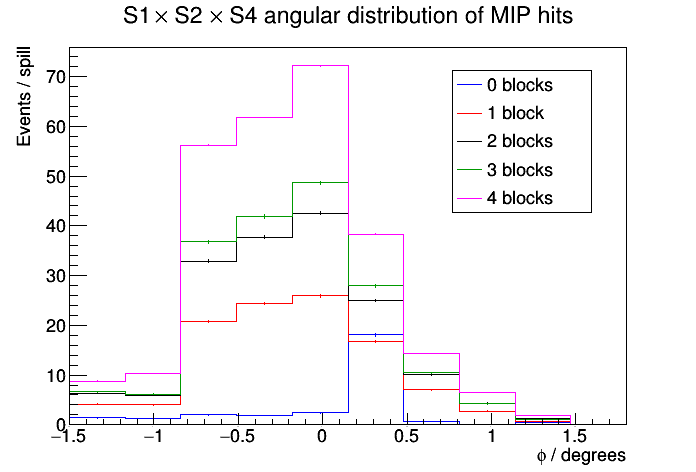
\includegraphics[width=\textwidth]{files/Figures/piS4Vert}
  %	\caption{Distribution of hits identified in $\mathit{S4}$ as minimum ionizing particles as a function of the number of moderator blocks and the vertical off-axis angle, as measured from $\mathit{S1}$.}
  %\end{minipage}
  %\hspace{0.3cm}
  %\begin{minipage}[t]{0.48\textwidth}
  %	\centering
  %	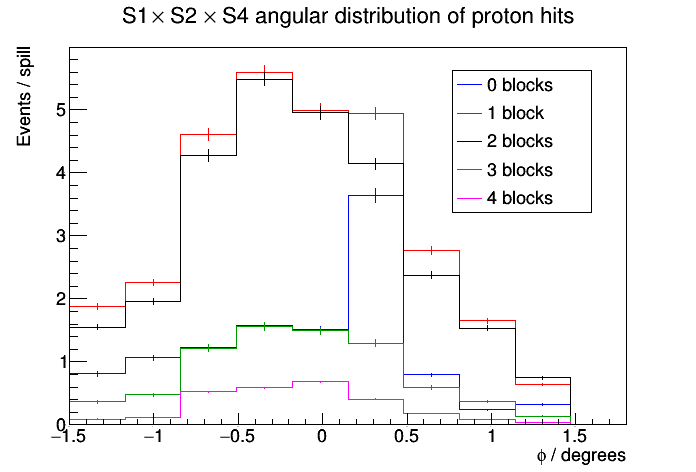
\includegraphics[width=\textwidth]{files/Figures/proS4Vert}
  %	\caption{Distribution of hits identified in $\mathit{S_{4}$ as protons as a function of the number of moderator blocks and the vertical off-axis angle, as measured from $\mathit{S_{1}$.}
  %\end{minipage}
\end{figure}	

Figures~\ref{fig:propiratio_s4_horz} and~\ref{fig:propiratio_s4_vert} show the ratio of protons to minimum ionizing particles as a function of the number of moderator blocks and the two off-axis angles.
\todo[inline]{JOCELYN: What are the two off-axis angles? Hard for the reader to figure out what the interesting region is. Need a figure that sets up the coordinate system}
For the 0, 1 and 2 moderator block configurations, figure~\ref{fig:propiratio_s4_horz} shows the ratio reaching its peak at a value of $\theta$ of approximately $2^{\circ}$.
It is clear that in the angular region of this peak, the proton-MIP ratio has been dramatically increased from the expected on axis value of 1:6 seen previously.
With the addition of moderator blocks, the size of the peak reduces until, in the 3 block configuration, the peak has fallen from a proton-MIP ratio of 1.1 for the 0 block configuration to value of 01. for the 3 block configuration. 
For the 4 block configuration, the proton-MIP ratio is below 0.05 for all values of $\theta$ but rises to its highest value at $\theta = 5^{\circ}$.

Similarly, figure~\ref{fig:propiratio_s4_vert} shows the proton-MIP ratio falling with the addition of moderator blocks.
\todo[inline]{JOCELYN: this whole discussion (and that of the previous paragraph is focussed on the proton-MIP ratio, however more important to the goals of the beamtest is to achieve low momentum proton flux to make measurements in the region relevant for neutrino-nucleus FSI.  Need to recast this whole discussion in terms of the goals: (1) proton momentum in the relevant range (2) low occupancy (<10 particles per spill in the TPC) given the relatively slow optical readout (3) proton-to-MIP ratio optimized}
For the 0, 1, 2 and 3 block configurations the ratio rises as the vertical off-axis angle ($\phi$) moves further away from $0^{\circ}$. 
For the 4 block configuration, the value of the proton-MIP ratio is close to zero at all values of $\phi$.
As mentioned previously, this is thought to be due to the attenuation of low energy protons within the walls of the pressure vessel.
\todo[inline]{Eliminate ``thought to be'' and put use the results of the simulation study to reinforce why we think this is.}

\begin{figure}[!ht]
  \begin{minipage}[t]{0.48\textwidth}
    \begin{adjustbox}{max totalsize={\textwidth}{.35\textheight}, center}
      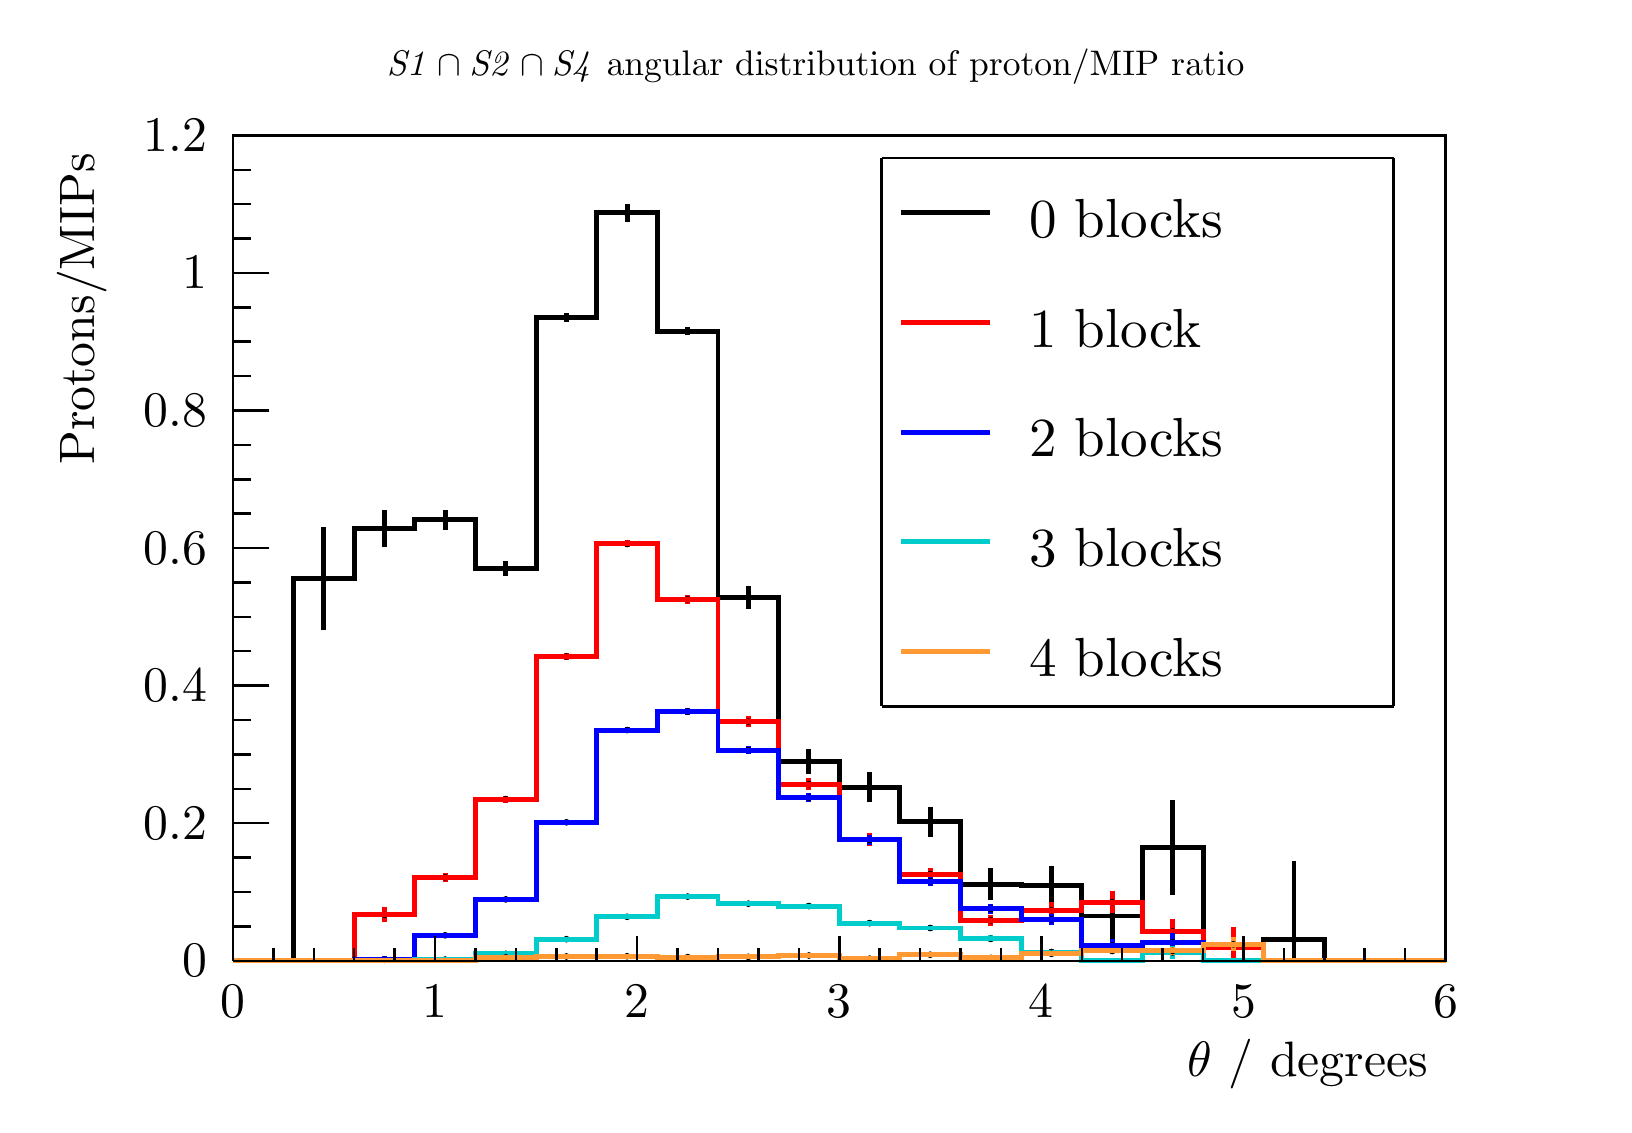
\begin{tikzpicture}
\pgfdeclareplotmark{cross} {
\pgfpathmoveto{\pgfpoint{-0.3\pgfplotmarksize}{\pgfplotmarksize}}
\pgfpathlineto{\pgfpoint{+0.3\pgfplotmarksize}{\pgfplotmarksize}}
\pgfpathlineto{\pgfpoint{+0.3\pgfplotmarksize}{0.3\pgfplotmarksize}}
\pgfpathlineto{\pgfpoint{+1\pgfplotmarksize}{0.3\pgfplotmarksize}}
\pgfpathlineto{\pgfpoint{+1\pgfplotmarksize}{-0.3\pgfplotmarksize}}
\pgfpathlineto{\pgfpoint{+0.3\pgfplotmarksize}{-0.3\pgfplotmarksize}}
\pgfpathlineto{\pgfpoint{+0.3\pgfplotmarksize}{-1.\pgfplotmarksize}}
\pgfpathlineto{\pgfpoint{-0.3\pgfplotmarksize}{-1.\pgfplotmarksize}}
\pgfpathlineto{\pgfpoint{-0.3\pgfplotmarksize}{-0.3\pgfplotmarksize}}
\pgfpathlineto{\pgfpoint{-1.\pgfplotmarksize}{-0.3\pgfplotmarksize}}
\pgfpathlineto{\pgfpoint{-1.\pgfplotmarksize}{0.3\pgfplotmarksize}}
\pgfpathlineto{\pgfpoint{-0.3\pgfplotmarksize}{0.3\pgfplotmarksize}}
\pgfpathclose
\pgfusepathqstroke
}
\pgfdeclareplotmark{cross*} {
\pgfpathmoveto{\pgfpoint{-0.3\pgfplotmarksize}{\pgfplotmarksize}}
\pgfpathlineto{\pgfpoint{+0.3\pgfplotmarksize}{\pgfplotmarksize}}
\pgfpathlineto{\pgfpoint{+0.3\pgfplotmarksize}{0.3\pgfplotmarksize}}
\pgfpathlineto{\pgfpoint{+1\pgfplotmarksize}{0.3\pgfplotmarksize}}
\pgfpathlineto{\pgfpoint{+1\pgfplotmarksize}{-0.3\pgfplotmarksize}}
\pgfpathlineto{\pgfpoint{+0.3\pgfplotmarksize}{-0.3\pgfplotmarksize}}
\pgfpathlineto{\pgfpoint{+0.3\pgfplotmarksize}{-1.\pgfplotmarksize}}
\pgfpathlineto{\pgfpoint{-0.3\pgfplotmarksize}{-1.\pgfplotmarksize}}
\pgfpathlineto{\pgfpoint{-0.3\pgfplotmarksize}{-0.3\pgfplotmarksize}}
\pgfpathlineto{\pgfpoint{-1.\pgfplotmarksize}{-0.3\pgfplotmarksize}}
\pgfpathlineto{\pgfpoint{-1.\pgfplotmarksize}{0.3\pgfplotmarksize}}
\pgfpathlineto{\pgfpoint{-0.3\pgfplotmarksize}{0.3\pgfplotmarksize}}
\pgfpathclose
\pgfusepathqfillstroke
}
\pgfdeclareplotmark{newstar} {
\pgfpathmoveto{\pgfqpoint{0pt}{\pgfplotmarksize}}
\pgfpathlineto{\pgfqpointpolar{44}{0.5\pgfplotmarksize}}
\pgfpathlineto{\pgfqpointpolar{18}{\pgfplotmarksize}}
\pgfpathlineto{\pgfqpointpolar{-20}{0.5\pgfplotmarksize}}
\pgfpathlineto{\pgfqpointpolar{-54}{\pgfplotmarksize}}
\pgfpathlineto{\pgfqpointpolar{-90}{0.5\pgfplotmarksize}}
\pgfpathlineto{\pgfqpointpolar{234}{\pgfplotmarksize}}
\pgfpathlineto{\pgfqpointpolar{198}{0.5\pgfplotmarksize}}
\pgfpathlineto{\pgfqpointpolar{162}{\pgfplotmarksize}}
\pgfpathlineto{\pgfqpointpolar{134}{0.5\pgfplotmarksize}}
\pgfpathclose
\pgfusepathqstroke
}
\pgfdeclareplotmark{newstar*} {
\pgfpathmoveto{\pgfqpoint{0pt}{\pgfplotmarksize}}
\pgfpathlineto{\pgfqpointpolar{44}{0.5\pgfplotmarksize}}
\pgfpathlineto{\pgfqpointpolar{18}{\pgfplotmarksize}}
\pgfpathlineto{\pgfqpointpolar{-20}{0.5\pgfplotmarksize}}
\pgfpathlineto{\pgfqpointpolar{-54}{\pgfplotmarksize}}
\pgfpathlineto{\pgfqpointpolar{-90}{0.5\pgfplotmarksize}}
\pgfpathlineto{\pgfqpointpolar{234}{\pgfplotmarksize}}
\pgfpathlineto{\pgfqpointpolar{198}{0.5\pgfplotmarksize}}
\pgfpathlineto{\pgfqpointpolar{162}{\pgfplotmarksize}}
\pgfpathlineto{\pgfqpointpolar{134}{0.5\pgfplotmarksize}}
\pgfpathclose
\pgfusepathqfillstroke
}
\definecolor{c}{rgb}{1,1,1};
\draw [color=c, fill=c] (0,0) rectangle (20,13.6127);
\draw [color=c, fill=c] (2.6,1.76965) rectangle (18,12.2514);
\definecolor{c}{rgb}{0,0,0};
\draw [c,line width=0.9] (2.6,1.76965) -- (2.6,12.2514) -- (18,12.2514) -- (18,1.76965) -- (2.6,1.76965);
\definecolor{c}{rgb}{1,1,1};
\draw [color=c, fill=c] (2.6,1.76965) rectangle (18,12.2514);
\definecolor{c}{rgb}{0,0,0};
\draw [c,line width=0.9] (2.6,1.76965) -- (2.6,12.2514) -- (18,12.2514) -- (18,1.76965) -- (2.6,1.76965);
\definecolor{c}{rgb}{0,0,0.6};
\draw [c,line width=0.9] (2.6,1.76965) -- (3.37,1.76965) -- (3.37,1.76965) -- (4.14,1.76965) -- (4.14,1.76965) -- (4.91,1.76965) -- (4.91,1.76965) -- (5.68,1.76965) -- (5.68,1.76965) -- (6.45,1.76965) -- (6.45,1.76965) -- (7.22,1.76965) --
 (7.22,1.76965) -- (7.99,1.76965) -- (7.99,1.76965) -- (8.76,1.76965) -- (8.76,1.76965) -- (9.53,1.76965) -- (9.53,1.76965) -- (10.3,1.76965) -- (10.3,1.76965) -- (11.07,1.76965) -- (11.07,1.76965) -- (11.84,1.76965) -- (11.84,1.76965) --
 (12.61,1.76965) -- (12.61,1.76965) -- (13.38,1.76965) -- (13.38,1.76965) -- (14.15,1.76965) -- (14.15,1.76965) -- (14.92,1.76965) -- (14.92,1.76965) -- (15.69,1.76965) -- (15.69,1.76965) -- (16.46,1.76965) -- (16.46,1.76965) -- (17.23,1.76965) --
 (17.23,1.76965) -- (18,1.76965);
\definecolor{c}{rgb}{0,0,0};
\draw [c,line width=0.9] (2.6,1.76965) -- (18,1.76965);
\draw [c,line width=0.9] (2.6,2.08411) -- (2.6,1.76965);
\draw [c,line width=0.9] (3.11333,1.92688) -- (3.11333,1.76965);
\draw [c,line width=0.9] (3.62667,1.92688) -- (3.62667,1.76965);
\draw [c,line width=0.9] (4.14,1.92688) -- (4.14,1.76965);
\draw [c,line width=0.9] (4.65333,1.92688) -- (4.65333,1.76965);
\draw [c,line width=0.9] (5.16667,2.08411) -- (5.16667,1.76965);
\draw [c,line width=0.9] (5.68,1.92688) -- (5.68,1.76965);
\draw [c,line width=0.9] (6.19333,1.92688) -- (6.19333,1.76965);
\draw [c,line width=0.9] (6.70667,1.92688) -- (6.70667,1.76965);
\draw [c,line width=0.9] (7.22,1.92688) -- (7.22,1.76965);
\draw [c,line width=0.9] (7.73333,2.08411) -- (7.73333,1.76965);
\draw [c,line width=0.9] (8.24667,1.92688) -- (8.24667,1.76965);
\draw [c,line width=0.9] (8.76,1.92688) -- (8.76,1.76965);
\draw [c,line width=0.9] (9.27333,1.92688) -- (9.27333,1.76965);
\draw [c,line width=0.9] (9.78667,1.92688) -- (9.78667,1.76965);
\draw [c,line width=0.9] (10.3,2.08411) -- (10.3,1.76965);
\draw [c,line width=0.9] (10.8133,1.92688) -- (10.8133,1.76965);
\draw [c,line width=0.9] (11.3267,1.92688) -- (11.3267,1.76965);
\draw [c,line width=0.9] (11.84,1.92688) -- (11.84,1.76965);
\draw [c,line width=0.9] (12.3533,1.92688) -- (12.3533,1.76965);
\draw [c,line width=0.9] (12.8667,2.08411) -- (12.8667,1.76965);
\draw [c,line width=0.9] (13.38,1.92688) -- (13.38,1.76965);
\draw [c,line width=0.9] (13.8933,1.92688) -- (13.8933,1.76965);
\draw [c,line width=0.9] (14.4067,1.92688) -- (14.4067,1.76965);
\draw [c,line width=0.9] (14.92,1.92688) -- (14.92,1.76965);
\draw [c,line width=0.9] (15.4333,2.08411) -- (15.4333,1.76965);
\draw [c,line width=0.9] (15.9467,1.92688) -- (15.9467,1.76965);
\draw [c,line width=0.9] (16.46,1.92688) -- (16.46,1.76965);
\draw [c,line width=0.9] (16.9733,1.92688) -- (16.9733,1.76965);
\draw [c,line width=0.9] (17.4867,1.92688) -- (17.4867,1.76965);
\draw [c,line width=0.9] (18,2.08411) -- (18,1.76965);
\draw [anchor=base] (2.6,1.04818) node[scale=1.79732, color=c, rotate=0]{0};
\draw [anchor=base] (5.16667,1.04818) node[scale=1.79732, color=c, rotate=0]{1};
\draw [anchor=base] (7.73333,1.04818) node[scale=1.79732, color=c, rotate=0]{2};
\draw [anchor=base] (10.3,1.04818) node[scale=1.79732, color=c, rotate=0]{3};
\draw [anchor=base] (12.8667,1.04818) node[scale=1.79732, color=c, rotate=0]{4};
\draw [anchor=base] (15.4333,1.04818) node[scale=1.79732, color=c, rotate=0]{5};
\draw [anchor=base] (18,1.04818) node[scale=1.79732, color=c, rotate=0]{6};
\draw [anchor= east] (18,0.462832) node[scale=1.79732, color=c, rotate=0]{$\theta$ / degrees};
\draw [c,line width=0.9] (2.6,1.76965) -- (2.6,12.2514);
\draw [c,line width=0.9] (3.062,1.76965) -- (2.6,1.76965);
\draw [c,line width=0.9] (2.831,2.20639) -- (2.6,2.20639);
\draw [c,line width=0.9] (2.831,2.64314) -- (2.6,2.64314);
\draw [c,line width=0.9] (2.831,3.07988) -- (2.6,3.07988);
\draw [c,line width=0.9] (3.062,3.51662) -- (2.6,3.51662);
\draw [c,line width=0.9] (2.831,3.95336) -- (2.6,3.95336);
\draw [c,line width=0.9] (2.831,4.3901) -- (2.6,4.3901);
\draw [c,line width=0.9] (2.831,4.82684) -- (2.6,4.82684);
\draw [c,line width=0.9] (3.062,5.26358) -- (2.6,5.26358);
\draw [c,line width=0.9] (2.831,5.70033) -- (2.6,5.70033);
\draw [c,line width=0.9] (2.831,6.13707) -- (2.6,6.13707);
\draw [c,line width=0.9] (2.831,6.57381) -- (2.6,6.57381);
\draw [c,line width=0.9] (3.062,7.01055) -- (2.6,7.01055);
\draw [c,line width=0.9] (2.831,7.44729) -- (2.6,7.44729);
\draw [c,line width=0.9] (2.831,7.88403) -- (2.6,7.88403);
\draw [c,line width=0.9] (2.831,8.32077) -- (2.6,8.32077);
\draw [c,line width=0.9] (3.062,8.75751) -- (2.6,8.75751);
\draw [c,line width=0.9] (2.831,9.19426) -- (2.6,9.19426);
\draw [c,line width=0.9] (2.831,9.631) -- (2.6,9.631);
\draw [c,line width=0.9] (2.831,10.0677) -- (2.6,10.0677);
\draw [c,line width=0.9] (3.062,10.5045) -- (2.6,10.5045);
\draw [c,line width=0.9] (2.831,10.9412) -- (2.6,10.9412);
\draw [c,line width=0.9] (2.831,11.378) -- (2.6,11.378);
\draw [c,line width=0.9] (2.831,11.8147) -- (2.6,11.8147);
\draw [c,line width=0.9] (3.062,12.2514) -- (2.6,12.2514);
\draw [c,line width=0.9] (3.062,12.2514) -- (2.6,12.2514);
\draw [anchor= east] (2.5,1.76965) node[scale=1.79732, color=c, rotate=0]{0};
\draw [anchor= east] (2.5,3.51662) node[scale=1.79732, color=c, rotate=0]{0.2};
\draw [anchor= east] (2.5,5.26358) node[scale=1.79732, color=c, rotate=0]{0.4};
\draw [anchor= east] (2.5,7.01055) node[scale=1.79732, color=c, rotate=0]{0.6};
\draw [anchor= east] (2.5,8.75751) node[scale=1.79732, color=c, rotate=0]{0.8};
\draw [anchor= east] (2.5,10.5045) node[scale=1.79732, color=c, rotate=0]{1};
\draw [anchor= east] (2.5,12.2514) node[scale=1.79732, color=c, rotate=0]{1.2};
\draw [anchor= east] (0.68,12.2514) node[scale=1.79732, color=c, rotate=90]{ Protons/MIPs};
\draw [c,line width=1.8] (3.755,5.96552) -- (3.755,6.61918);
\draw [c,line width=1.8] (3.755,6.61918) -- (3.755,7.27284);
\foreach \P in {(3.755,6.61918)}{\draw[mark options={color=c,fill=c},mark size=2.402402pt,mark=*,mark size=1pt] plot coordinates {\P};}
\draw [c,line width=1.8] (4.525,7.02017) -- (4.525,7.25485);
\draw [c,line width=1.8] (4.525,7.25485) -- (4.525,7.48953);
\foreach \P in {(4.525,7.25485)}{\draw[mark options={color=c,fill=c},mark size=2.402402pt,mark=*,mark size=1pt] plot coordinates {\P};}
\draw [c,line width=1.8] (5.295,7.24454) -- (5.295,7.36993);
\draw [c,line width=1.8] (5.295,7.36993) -- (5.295,7.49531);
\foreach \P in {(5.295,7.36993)}{\draw[mark options={color=c,fill=c},mark size=2.402402pt,mark=*,mark size=1pt] plot coordinates {\P};}
\draw [c,line width=1.8] (6.065,6.65801) -- (6.065,6.75329);
\draw [c,line width=1.8] (6.065,6.75329) -- (6.065,6.84857);
\foreach \P in {(6.065,6.75329)}{\draw[mark options={color=c,fill=c},mark size=2.402402pt,mark=*,mark size=1pt] plot coordinates {\P};}
\draw [c,line width=1.8] (6.835,9.88682) -- (6.835,9.94428);
\draw [c,line width=1.8] (6.835,9.94428) -- (6.835,10.0017);
\foreach \P in {(6.835,9.94428)}{\draw[mark options={color=c,fill=c},mark size=2.402402pt,mark=*,mark size=1pt] plot coordinates {\P};}
\draw [c,line width=1.8] (7.605,11.157) -- (7.605,11.267);
\draw [c,line width=1.8] (7.605,11.267) -- (7.605,11.3769);
\foreach \P in {(7.605,11.267)}{\draw[mark options={color=c,fill=c},mark size=2.402402pt,mark=*,mark size=1pt] plot coordinates {\P};}
\draw [c,line width=1.8] (8.375,9.71118) -- (8.375,9.76656);
\draw [c,line width=1.8] (8.375,9.76656) -- (8.375,9.82195);
\foreach \P in {(8.375,9.76656)}{\draw[mark options={color=c,fill=c},mark size=2.402402pt,mark=*,mark size=1pt] plot coordinates {\P};}
\draw [c,line width=1.8] (9.145,6.23982) -- (9.145,6.3858);
\draw [c,line width=1.8] (9.145,6.3858) -- (9.145,6.53178);
\foreach \P in {(9.145,6.3858)}{\draw[mark options={color=c,fill=c},mark size=2.402402pt,mark=*,mark size=1pt] plot coordinates {\P};}
\draw [c,line width=1.8] (9.915,4.14538) -- (9.915,4.30397);
\draw [c,line width=1.8] (9.915,4.30397) -- (9.915,4.46257);
\foreach \P in {(9.915,4.30397)}{\draw[mark options={color=c,fill=c},mark size=2.402402pt,mark=*,mark size=1pt] plot coordinates {\P};}
\draw [c,line width=1.8] (10.685,3.78343) -- (10.685,3.9732);
\draw [c,line width=1.8] (10.685,3.9732) -- (10.685,4.16297);
\foreach \P in {(10.685,3.9732)}{\draw[mark options={color=c,fill=c},mark size=2.402402pt,mark=*,mark size=1pt] plot coordinates {\P};}
\draw [c,line width=1.8] (11.455,3.3397) -- (11.455,3.53224);
\draw [c,line width=1.8] (11.455,3.53224) -- (11.455,3.72478);
\foreach \P in {(11.455,3.53224)}{\draw[mark options={color=c,fill=c},mark size=2.402402pt,mark=*,mark size=1pt] plot coordinates {\P};}
\draw [c,line width=1.8] (12.225,2.53805) -- (12.225,2.74072);
\draw [c,line width=1.8] (12.225,2.74072) -- (12.225,2.94338);
\foreach \P in {(12.225,2.74072)}{\draw[mark options={color=c,fill=c},mark size=2.402402pt,mark=*,mark size=1pt] plot coordinates {\P};}
\draw [c,line width=1.8] (12.995,2.48276) -- (12.995,2.72628);
\draw [c,line width=1.8] (12.995,2.72628) -- (12.995,2.9698);
\foreach \P in {(12.995,2.72628)}{\draw[mark options={color=c,fill=c},mark size=2.402402pt,mark=*,mark size=1pt] plot coordinates {\P};}
\draw [c,line width=1.8] (13.765,2.01881) -- (13.765,2.3379);
\draw [c,line width=1.8] (13.765,2.3379) -- (13.765,2.65699);
\foreach \P in {(13.765,2.3379)}{\draw[mark options={color=c,fill=c},mark size=2.402402pt,mark=*,mark size=1pt] plot coordinates {\P};}
\draw [c,line width=1.8] (14.535,2.60709) -- (14.535,3.20937);
\draw [c,line width=1.8] (14.535,3.20937) -- (14.535,3.81165);
\foreach \P in {(14.535,3.20937)}{\draw[mark options={color=c,fill=c},mark size=2.402402pt,mark=*,mark size=1pt] plot coordinates {\P};}
\draw [c,line width=1.8] (16.075,1.76965) -- (16.075,2.03461);
\draw [c,line width=1.8] (16.075,2.03461) -- (16.075,3.04084);
\foreach \P in {(16.075,2.03461)}{\draw[mark options={color=c,fill=c},mark size=2.402402pt,mark=*,mark size=1pt] plot coordinates {\P};}
\draw [c,line width=1.8] (2.6,1.76965) -- (3.37,1.76965) -- (3.37,6.61918) -- (4.14,6.61918) -- (4.14,7.25485) -- (4.91,7.25485) -- (4.91,7.36993) -- (5.68,7.36993) -- (5.68,6.75329) -- (6.45,6.75329) -- (6.45,9.94428) -- (7.22,9.94428) --
 (7.22,11.267) -- (7.99,11.267) -- (7.99,9.76656) -- (8.76,9.76656) -- (8.76,6.3858) -- (9.53,6.3858) -- (9.53,4.30397) -- (10.3,4.30397) -- (10.3,3.9732) -- (11.07,3.9732) -- (11.07,3.53224) -- (11.84,3.53224) -- (11.84,2.74072) -- (12.61,2.74072)
 -- (12.61,2.72628) -- (13.38,2.72628) -- (13.38,2.3379) -- (14.15,2.3379) -- (14.15,3.20937) -- (14.92,3.20937) -- (14.92,1.76965) -- (15.69,1.76965) -- (15.69,2.03461) -- (16.46,2.03461) -- (16.46,1.76965) -- (17.23,1.76965) -- (17.23,1.76965) --
 (18,1.76965);
\definecolor{c}{rgb}{1,0,0};
\draw [c,line width=1.8] (4.525,2.25718) -- (4.525,2.35159);
\draw [c,line width=1.8] (4.525,2.35159) -- (4.525,2.446);
\definecolor{c}{rgb}{0,0,0};
\foreach \P in {(4.525,2.35159)}{\draw[mark options={color=c,fill=c},mark size=2.402402pt,mark=*,mark size=1pt] plot coordinates {\P};}
\definecolor{c}{rgb}{1,0,0};
\draw [c,line width=1.8] (5.295,2.77091) -- (5.295,2.82905);
\draw [c,line width=1.8] (5.295,2.82905) -- (5.295,2.88719);
\definecolor{c}{rgb}{0,0,0};
\foreach \P in {(5.295,2.82905)}{\draw[mark options={color=c,fill=c},mark size=2.402402pt,mark=*,mark size=1pt] plot coordinates {\P};}
\definecolor{c}{rgb}{1,0,0};
\draw [c,line width=1.8] (6.065,3.77647) -- (6.065,3.82233);
\draw [c,line width=1.8] (6.065,3.82233) -- (6.065,3.86819);
\definecolor{c}{rgb}{0,0,0};
\foreach \P in {(6.065,3.82233)}{\draw[mark options={color=c,fill=c},mark size=2.402402pt,mark=*,mark size=1pt] plot coordinates {\P};}
\definecolor{c}{rgb}{1,0,0};
\draw [c,line width=1.8] (6.835,5.59037) -- (6.835,5.63438);
\draw [c,line width=1.8] (6.835,5.63438) -- (6.835,5.67838);
\definecolor{c}{rgb}{0,0,0};
\foreach \P in {(6.835,5.63438)}{\draw[mark options={color=c,fill=c},mark size=2.402402pt,mark=*,mark size=1pt] plot coordinates {\P};}
\definecolor{c}{rgb}{1,0,0};
\draw [c,line width=1.8] (7.605,7.01849) -- (7.605,7.06322);
\draw [c,line width=1.8] (7.605,7.06322) -- (7.605,7.10796);
\definecolor{c}{rgb}{0,0,0};
\foreach \P in {(7.605,7.06322)}{\draw[mark options={color=c,fill=c},mark size=2.402402pt,mark=*,mark size=1pt] plot coordinates {\P};}
\definecolor{c}{rgb}{1,0,0};
\draw [c,line width=1.8] (8.375,6.30504) -- (8.375,6.36061);
\draw [c,line width=1.8] (8.375,6.36061) -- (8.375,6.41618);
\definecolor{c}{rgb}{0,0,0};
\foreach \P in {(8.375,6.36061)}{\draw[mark options={color=c,fill=c},mark size=2.402402pt,mark=*,mark size=1pt] plot coordinates {\P};}
\definecolor{c}{rgb}{1,0,0};
\draw [c,line width=1.8] (9.145,4.73795) -- (9.145,4.80704);
\draw [c,line width=1.8] (9.145,4.80704) -- (9.145,4.87612);
\definecolor{c}{rgb}{0,0,0};
\foreach \P in {(9.145,4.80704)}{\draw[mark options={color=c,fill=c},mark size=2.402402pt,mark=*,mark size=1pt] plot coordinates {\P};}
\definecolor{c}{rgb}{1,0,0};
\draw [c,line width=1.8] (9.915,3.93827) -- (9.915,4.01338);
\draw [c,line width=1.8] (9.915,4.01338) -- (9.915,4.08848);
\definecolor{c}{rgb}{0,0,0};
\foreach \P in {(9.915,4.01338)}{\draw[mark options={color=c,fill=c},mark size=2.402402pt,mark=*,mark size=1pt] plot coordinates {\P};}
\definecolor{c}{rgb}{1,0,0};
\draw [c,line width=1.8] (10.685,3.22568) -- (10.685,3.30686);
\draw [c,line width=1.8] (10.685,3.30686) -- (10.685,3.38804);
\definecolor{c}{rgb}{0,0,0};
\foreach \P in {(10.685,3.30686)}{\draw[mark options={color=c,fill=c},mark size=2.402402pt,mark=*,mark size=1pt] plot coordinates {\P};}
\definecolor{c}{rgb}{1,0,0};
\draw [c,line width=1.8] (11.455,2.78746) -- (11.455,2.87067);
\draw [c,line width=1.8] (11.455,2.87067) -- (11.455,2.95388);
\definecolor{c}{rgb}{0,0,0};
\foreach \P in {(11.455,2.87067)}{\draw[mark options={color=c,fill=c},mark size=2.402402pt,mark=*,mark size=1pt] plot coordinates {\P};}
\definecolor{c}{rgb}{1,0,0};
\draw [c,line width=1.8] (12.225,2.21253) -- (12.225,2.28363);
\draw [c,line width=1.8] (12.225,2.28363) -- (12.225,2.35473);
\definecolor{c}{rgb}{0,0,0};
\foreach \P in {(12.225,2.28363)}{\draw[mark options={color=c,fill=c},mark size=2.402402pt,mark=*,mark size=1pt] plot coordinates {\P};}
\definecolor{c}{rgb}{1,0,0};
\draw [c,line width=1.8] (12.995,2.30897) -- (12.995,2.41012);
\draw [c,line width=1.8] (12.995,2.41012) -- (12.995,2.51127);
\definecolor{c}{rgb}{0,0,0};
\foreach \P in {(12.995,2.41012)}{\draw[mark options={color=c,fill=c},mark size=2.402402pt,mark=*,mark size=1pt] plot coordinates {\P};}
\definecolor{c}{rgb}{1,0,0};
\draw [c,line width=1.8] (13.765,2.37186) -- (13.765,2.51465);
\draw [c,line width=1.8] (13.765,2.51465) -- (13.765,2.65744);
\definecolor{c}{rgb}{0,0,0};
\foreach \P in {(13.765,2.51465)}{\draw[mark options={color=c,fill=c},mark size=2.402402pt,mark=*,mark size=1pt] plot coordinates {\P};}
\definecolor{c}{rgb}{1,0,0};
\draw [c,line width=1.8] (14.535,1.98578) -- (14.535,2.14154);
\draw [c,line width=1.8] (14.535,2.14154) -- (14.535,2.29731);
\definecolor{c}{rgb}{0,0,0};
\foreach \P in {(14.535,2.14154)}{\draw[mark options={color=c,fill=c},mark size=2.402402pt,mark=*,mark size=1pt] plot coordinates {\P};}
\definecolor{c}{rgb}{1,0,0};
\draw [c,line width=1.8] (15.305,1.76965) -- (15.305,1.94371);
\draw [c,line width=1.8] (15.305,1.94371) -- (15.305,2.19744);
\definecolor{c}{rgb}{0,0,0};
\foreach \P in {(15.305,1.94371)}{\draw[mark options={color=c,fill=c},mark size=2.402402pt,mark=*,mark size=1pt] plot coordinates {\P};}
\definecolor{c}{rgb}{1,0,0};
\draw [c,line width=1.8] (2.6,1.76965) -- (3.37,1.76965) -- (3.37,1.76965) -- (4.14,1.76965) -- (4.14,2.35159) -- (4.91,2.35159) -- (4.91,2.82905) -- (5.68,2.82905) -- (5.68,3.82233) -- (6.45,3.82233) -- (6.45,5.63438) -- (7.22,5.63438) --
 (7.22,7.06322) -- (7.99,7.06322) -- (7.99,6.36061) -- (8.76,6.36061) -- (8.76,4.80704) -- (9.53,4.80704) -- (9.53,4.01338) -- (10.3,4.01338) -- (10.3,3.30686) -- (11.07,3.30686) -- (11.07,2.87067) -- (11.84,2.87067) -- (11.84,2.28363) --
 (12.61,2.28363) -- (12.61,2.41012) -- (13.38,2.41012) -- (13.38,2.51465) -- (14.15,2.51465) -- (14.15,2.14154) -- (14.92,2.14154) -- (14.92,1.94371) -- (15.69,1.94371) -- (15.69,1.76965) -- (16.46,1.76965) -- (16.46,1.76965) -- (17.23,1.76965) --
 (17.23,1.76965) -- (18,1.76965);
\definecolor{c}{rgb}{0,0,1};
\draw [c,line width=1.8] (4.525,1.76965) -- (4.525,1.7823);
\draw [c,line width=1.8] (4.525,1.7823) -- (4.525,1.83564);
\definecolor{c}{rgb}{0,0,0};
\foreach \P in {(4.525,1.7823)}{\draw[mark options={color=c,fill=c},mark size=2.402402pt,mark=*,mark size=1pt] plot coordinates {\P};}
\definecolor{c}{rgb}{0,0,1};
\draw [c,line width=1.8] (5.295,2.06026) -- (5.295,2.09298);
\draw [c,line width=1.8] (5.295,2.09298) -- (5.295,2.12571);
\definecolor{c}{rgb}{0,0,0};
\foreach \P in {(5.295,2.09298)}{\draw[mark options={color=c,fill=c},mark size=2.402402pt,mark=*,mark size=1pt] plot coordinates {\P};}
\definecolor{c}{rgb}{0,0,1};
\draw [c,line width=1.8] (6.065,2.5215) -- (6.065,2.54923);
\draw [c,line width=1.8] (6.065,2.54923) -- (6.065,2.57695);
\definecolor{c}{rgb}{0,0,0};
\foreach \P in {(6.065,2.54923)}{\draw[mark options={color=c,fill=c},mark size=2.402402pt,mark=*,mark size=1pt] plot coordinates {\P};}
\definecolor{c}{rgb}{0,0,1};
\draw [c,line width=1.8] (6.835,3.49681) -- (6.835,3.52792);
\draw [c,line width=1.8] (6.835,3.52792) -- (6.835,3.55903);
\definecolor{c}{rgb}{0,0,0};
\foreach \P in {(6.835,3.52792)}{\draw[mark options={color=c,fill=c},mark size=2.402402pt,mark=*,mark size=1pt] plot coordinates {\P};}
\definecolor{c}{rgb}{0,0,1};
\draw [c,line width=1.8] (7.605,4.66274) -- (7.605,4.69928);
\draw [c,line width=1.8] (7.605,4.69928) -- (7.605,4.73582);
\definecolor{c}{rgb}{0,0,0};
\foreach \P in {(7.605,4.69928)}{\draw[mark options={color=c,fill=c},mark size=2.402402pt,mark=*,mark size=1pt] plot coordinates {\P};}
\definecolor{c}{rgb}{0,0,1};
\draw [c,line width=1.8] (8.375,4.89186) -- (8.375,4.93533);
\draw [c,line width=1.8] (8.375,4.93533) -- (8.375,4.9788);
\definecolor{c}{rgb}{0,0,0};
\foreach \P in {(8.375,4.93533)}{\draw[mark options={color=c,fill=c},mark size=2.402402pt,mark=*,mark size=1pt] plot coordinates {\P};}
\definecolor{c}{rgb}{0,0,1};
\draw [c,line width=1.8] (9.145,4.39433) -- (9.145,4.44478);
\draw [c,line width=1.8] (9.145,4.44478) -- (9.145,4.49524);
\definecolor{c}{rgb}{0,0,0};
\foreach \P in {(9.145,4.44478)}{\draw[mark options={color=c,fill=c},mark size=2.402402pt,mark=*,mark size=1pt] plot coordinates {\P};}
\definecolor{c}{rgb}{0,0,1};
\draw [c,line width=1.8] (9.915,3.78582) -- (9.915,3.84078);
\draw [c,line width=1.8] (9.915,3.84078) -- (9.915,3.89575);
\definecolor{c}{rgb}{0,0,0};
\foreach \P in {(9.915,3.84078)}{\draw[mark options={color=c,fill=c},mark size=2.402402pt,mark=*,mark size=1pt] plot coordinates {\P};}
\definecolor{c}{rgb}{0,0,1};
\draw [c,line width=1.8] (10.685,3.24461) -- (10.685,3.3036);
\draw [c,line width=1.8] (10.685,3.3036) -- (10.685,3.36259);
\definecolor{c}{rgb}{0,0,0};
\foreach \P in {(10.685,3.3036)}{\draw[mark options={color=c,fill=c},mark size=2.402402pt,mark=*,mark size=1pt] plot coordinates {\P};}
\definecolor{c}{rgb}{0,0,1};
\draw [c,line width=1.8] (11.455,2.72135) -- (11.455,2.77999);
\draw [c,line width=1.8] (11.455,2.77999) -- (11.455,2.83863);
\definecolor{c}{rgb}{0,0,0};
\foreach \P in {(11.455,2.77999)}{\draw[mark options={color=c,fill=c},mark size=2.402402pt,mark=*,mark size=1pt] plot coordinates {\P};}
\definecolor{c}{rgb}{0,0,1};
\draw [c,line width=1.8] (12.225,2.36619) -- (12.225,2.42732);
\draw [c,line width=1.8] (12.225,2.42732) -- (12.225,2.48844);
\definecolor{c}{rgb}{0,0,0};
\foreach \P in {(12.225,2.42732)}{\draw[mark options={color=c,fill=c},mark size=2.402402pt,mark=*,mark size=1pt] plot coordinates {\P};}
\definecolor{c}{rgb}{0,0,1};
\draw [c,line width=1.8] (12.995,2.22581) -- (12.995,2.29456);
\draw [c,line width=1.8] (12.995,2.29456) -- (12.995,2.36332);
\definecolor{c}{rgb}{0,0,0};
\foreach \P in {(12.995,2.29456)}{\draw[mark options={color=c,fill=c},mark size=2.402402pt,mark=*,mark size=1pt] plot coordinates {\P};}
\definecolor{c}{rgb}{0,0,1};
\draw [c,line width=1.8] (13.765,1.88797) -- (13.765,1.96423);
\draw [c,line width=1.8] (13.765,1.96423) -- (13.765,2.04048);
\definecolor{c}{rgb}{0,0,0};
\foreach \P in {(13.765,1.96423)}{\draw[mark options={color=c,fill=c},mark size=2.402402pt,mark=*,mark size=1pt] plot coordinates {\P};}
\definecolor{c}{rgb}{0,0,1};
\draw [c,line width=1.8] (14.535,1.88836) -- (14.535,2.00549);
\draw [c,line width=1.8] (14.535,2.00549) -- (14.535,2.12261);
\definecolor{c}{rgb}{0,0,0};
\foreach \P in {(14.535,2.00549)}{\draw[mark options={color=c,fill=c},mark size=2.402402pt,mark=*,mark size=1pt] plot coordinates {\P};}
\definecolor{c}{rgb}{0,0,1};
\draw [c,line width=1.8] (2.6,1.76965) -- (3.37,1.76965) -- (3.37,1.76965) -- (4.14,1.76965) -- (4.14,1.7823) -- (4.91,1.7823) -- (4.91,2.09298) -- (5.68,2.09298) -- (5.68,2.54923) -- (6.45,2.54923) -- (6.45,3.52792) -- (7.22,3.52792) --
 (7.22,4.69928) -- (7.99,4.69928) -- (7.99,4.93533) -- (8.76,4.93533) -- (8.76,4.44478) -- (9.53,4.44478) -- (9.53,3.84078) -- (10.3,3.84078) -- (10.3,3.3036) -- (11.07,3.3036) -- (11.07,2.77999) -- (11.84,2.77999) -- (11.84,2.42732) --
 (12.61,2.42732) -- (12.61,2.29456) -- (13.38,2.29456) -- (13.38,1.96423) -- (14.15,1.96423) -- (14.15,2.00549) -- (14.92,2.00549) -- (14.92,1.76965) -- (15.69,1.76965) -- (15.69,1.76965) -- (16.46,1.76965) -- (16.46,1.76965) -- (17.23,1.76965) --
 (17.23,1.76965) -- (18,1.76965);
\definecolor{c}{rgb}{0,0.8,0.8};
\draw [c,line width=1.8] (5.295,1.76965) -- (5.295,1.78457);
\draw [c,line width=1.8] (5.295,1.78457) -- (5.295,1.80271);
\definecolor{c}{rgb}{0,0,0};
\foreach \P in {(5.295,1.78457)}{\draw[mark options={color=c,fill=c},mark size=2.402402pt,mark=*,mark size=1pt] plot coordinates {\P};}
\definecolor{c}{rgb}{0,0.8,0.8};
\draw [c,line width=1.8] (6.065,1.8446) -- (6.065,1.8573);
\draw [c,line width=1.8] (6.065,1.8573) -- (6.065,1.87);
\definecolor{c}{rgb}{0,0,0};
\foreach \P in {(6.065,1.8573)}{\draw[mark options={color=c,fill=c},mark size=2.402402pt,mark=*,mark size=1pt] plot coordinates {\P};}
\definecolor{c}{rgb}{0,0.8,0.8};
\draw [c,line width=1.8] (6.835,2.02672) -- (6.835,2.04365);
\draw [c,line width=1.8] (6.835,2.04365) -- (6.835,2.06058);
\definecolor{c}{rgb}{0,0,0};
\foreach \P in {(6.835,2.04365)}{\draw[mark options={color=c,fill=c},mark size=2.402402pt,mark=*,mark size=1pt] plot coordinates {\P};}
\definecolor{c}{rgb}{0,0.8,0.8};
\draw [c,line width=1.8] (7.605,2.30633) -- (7.605,2.32789);
\draw [c,line width=1.8] (7.605,2.32789) -- (7.605,2.34945);
\definecolor{c}{rgb}{0,0,0};
\foreach \P in {(7.605,2.32789)}{\draw[mark options={color=c,fill=c},mark size=2.402402pt,mark=*,mark size=1pt] plot coordinates {\P};}
\definecolor{c}{rgb}{0,0.8,0.8};
\draw [c,line width=1.8] (8.375,2.55536) -- (8.375,2.58455);
\draw [c,line width=1.8] (8.375,2.58455) -- (8.375,2.61374);
\definecolor{c}{rgb}{0,0,0};
\foreach \P in {(8.375,2.58455)}{\draw[mark options={color=c,fill=c},mark size=2.402402pt,mark=*,mark size=1pt] plot coordinates {\P};}
\definecolor{c}{rgb}{0,0.8,0.8};
\draw [c,line width=1.8] (9.145,2.46079) -- (9.145,2.49448);
\draw [c,line width=1.8] (9.145,2.49448) -- (9.145,2.52816);
\definecolor{c}{rgb}{0,0,0};
\foreach \P in {(9.145,2.49448)}{\draw[mark options={color=c,fill=c},mark size=2.402402pt,mark=*,mark size=1pt] plot coordinates {\P};}
\definecolor{c}{rgb}{0,0.8,0.8};
\draw [c,line width=1.8] (9.915,2.42409) -- (9.915,2.46387);
\draw [c,line width=1.8] (9.915,2.46387) -- (9.915,2.50366);
\definecolor{c}{rgb}{0,0,0};
\foreach \P in {(9.915,2.46387)}{\draw[mark options={color=c,fill=c},mark size=2.402402pt,mark=*,mark size=1pt] plot coordinates {\P};}
\definecolor{c}{rgb}{0,0.8,0.8};
\draw [c,line width=1.8] (10.685,2.20946) -- (10.685,2.2468);
\draw [c,line width=1.8] (10.685,2.2468) -- (10.685,2.28414);
\definecolor{c}{rgb}{0,0,0};
\foreach \P in {(10.685,2.2468)}{\draw[mark options={color=c,fill=c},mark size=2.402402pt,mark=*,mark size=1pt] plot coordinates {\P};}
\definecolor{c}{rgb}{0,0.8,0.8};
\draw [c,line width=1.8] (11.455,2.14459) -- (11.455,2.18563);
\draw [c,line width=1.8] (11.455,2.18563) -- (11.455,2.22667);
\definecolor{c}{rgb}{0,0,0};
\foreach \P in {(11.455,2.18563)}{\draw[mark options={color=c,fill=c},mark size=2.402402pt,mark=*,mark size=1pt] plot coordinates {\P};}
\definecolor{c}{rgb}{0,0.8,0.8};
\draw [c,line width=1.8] (12.225,2.00237) -- (12.225,2.0483);
\draw [c,line width=1.8] (12.225,2.0483) -- (12.225,2.09422);
\definecolor{c}{rgb}{0,0,0};
\foreach \P in {(12.225,2.0483)}{\draw[mark options={color=c,fill=c},mark size=2.402402pt,mark=*,mark size=1pt] plot coordinates {\P};}
\definecolor{c}{rgb}{0,0.8,0.8};
\draw [c,line width=1.8] (12.995,1.8366) -- (12.995,1.8805);
\draw [c,line width=1.8] (12.995,1.8805) -- (12.995,1.92441);
\definecolor{c}{rgb}{0,0,0};
\foreach \P in {(12.995,1.8805)}{\draw[mark options={color=c,fill=c},mark size=2.402402pt,mark=*,mark size=1pt] plot coordinates {\P};}
\definecolor{c}{rgb}{0,0.8,0.8};
\draw [c,line width=1.8] (14.535,1.78926) -- (14.535,1.8749);
\draw [c,line width=1.8] (14.535,1.8749) -- (14.535,1.96054);
\definecolor{c}{rgb}{0,0,0};
\foreach \P in {(14.535,1.8749)}{\draw[mark options={color=c,fill=c},mark size=2.402402pt,mark=*,mark size=1pt] plot coordinates {\P};}
\definecolor{c}{rgb}{0,0.8,0.8};
\draw [c,line width=1.8] (2.6,1.76965) -- (3.37,1.76965) -- (3.37,1.76965) -- (4.14,1.76965) -- (4.14,1.76965) -- (4.91,1.76965) -- (4.91,1.78457) -- (5.68,1.78457) -- (5.68,1.8573) -- (6.45,1.8573) -- (6.45,2.04365) -- (7.22,2.04365) --
 (7.22,2.32789) -- (7.99,2.32789) -- (7.99,2.58455) -- (8.76,2.58455) -- (8.76,2.49448) -- (9.53,2.49448) -- (9.53,2.46387) -- (10.3,2.46387) -- (10.3,2.2468) -- (11.07,2.2468) -- (11.07,2.18563) -- (11.84,2.18563) -- (11.84,2.0483) -- (12.61,2.0483)
 -- (12.61,1.8805) -- (13.38,1.8805) -- (13.38,1.76965) -- (14.15,1.76965) -- (14.15,1.8749) -- (14.92,1.8749) -- (14.92,1.76965) -- (15.69,1.76965) -- (15.69,1.76965) -- (16.46,1.76965) -- (16.46,1.76965) -- (17.23,1.76965) -- (17.23,1.76965) --
 (18,1.76965);
\definecolor{c}{rgb}{1,0.6,0.2};
\draw [c,line width=1.8] (6.065,1.8082) -- (6.065,1.81294);
\draw [c,line width=1.8] (6.065,1.81294) -- (6.065,1.81769);
\definecolor{c}{rgb}{0,0,0};
\foreach \P in {(6.065,1.81294)}{\draw[mark options={color=c,fill=c},mark size=2.402402pt,mark=*,mark size=1pt] plot coordinates {\P};}
\definecolor{c}{rgb}{1,0.6,0.2};
\draw [c,line width=1.8] (6.835,1.81861) -- (6.835,1.82418);
\draw [c,line width=1.8] (6.835,1.82418) -- (6.835,1.82974);
\definecolor{c}{rgb}{0,0,0};
\foreach \P in {(6.835,1.82418)}{\draw[mark options={color=c,fill=c},mark size=2.402402pt,mark=*,mark size=1pt] plot coordinates {\P};}
\definecolor{c}{rgb}{1,0.6,0.2};
\draw [c,line width=1.8] (7.605,1.822) -- (7.605,1.82706);
\draw [c,line width=1.8] (7.605,1.82706) -- (7.605,1.83212);
\definecolor{c}{rgb}{0,0,0};
\foreach \P in {(7.605,1.82706)}{\draw[mark options={color=c,fill=c},mark size=2.402402pt,mark=*,mark size=1pt] plot coordinates {\P};}
\definecolor{c}{rgb}{1,0.6,0.2};
\draw [c,line width=1.8] (8.375,1.81073) -- (8.375,1.8155);
\draw [c,line width=1.8] (8.375,1.8155) -- (8.375,1.82027);
\definecolor{c}{rgb}{0,0,0};
\foreach \P in {(8.375,1.8155)}{\draw[mark options={color=c,fill=c},mark size=2.402402pt,mark=*,mark size=1pt] plot coordinates {\P};}
\definecolor{c}{rgb}{1,0.6,0.2};
\draw [c,line width=1.8] (9.145,1.81131) -- (9.145,1.81903);
\draw [c,line width=1.8] (9.145,1.81903) -- (9.145,1.82675);
\definecolor{c}{rgb}{0,0,0};
\foreach \P in {(9.145,1.81903)}{\draw[mark options={color=c,fill=c},mark size=2.402402pt,mark=*,mark size=1pt] plot coordinates {\P};}
\definecolor{c}{rgb}{1,0.6,0.2};
\draw [c,line width=1.8] (9.915,1.82508) -- (9.915,1.83644);
\draw [c,line width=1.8] (9.915,1.83644) -- (9.915,1.8478);
\definecolor{c}{rgb}{0,0,0};
\foreach \P in {(9.915,1.83644)}{\draw[mark options={color=c,fill=c},mark size=2.402402pt,mark=*,mark size=1pt] plot coordinates {\P};}
\definecolor{c}{rgb}{1,0.6,0.2};
\draw [c,line width=1.8] (10.685,1.79053) -- (10.685,1.79625);
\draw [c,line width=1.8] (10.685,1.79625) -- (10.685,1.80197);
\definecolor{c}{rgb}{0,0,0};
\foreach \P in {(10.685,1.79625)}{\draw[mark options={color=c,fill=c},mark size=2.402402pt,mark=*,mark size=1pt] plot coordinates {\P};}
\definecolor{c}{rgb}{1,0.6,0.2};
\draw [c,line width=1.8] (11.455,1.83001) -- (11.455,1.84612);
\draw [c,line width=1.8] (11.455,1.84612) -- (11.455,1.86223);
\definecolor{c}{rgb}{0,0,0};
\foreach \P in {(11.455,1.84612)}{\draw[mark options={color=c,fill=c},mark size=2.402402pt,mark=*,mark size=1pt] plot coordinates {\P};}
\definecolor{c}{rgb}{1,0.6,0.2};
\draw [c,line width=1.8] (12.225,1.78986) -- (12.225,1.80562);
\draw [c,line width=1.8] (12.225,1.80562) -- (12.225,1.82137);
\definecolor{c}{rgb}{0,0,0};
\foreach \P in {(12.225,1.80562)}{\draw[mark options={color=c,fill=c},mark size=2.402402pt,mark=*,mark size=1pt] plot coordinates {\P};}
\definecolor{c}{rgb}{1,0.6,0.2};
\draw [c,line width=1.8] (12.995,1.82889) -- (12.995,1.85773);
\draw [c,line width=1.8] (12.995,1.85773) -- (12.995,1.88657);
\definecolor{c}{rgb}{0,0,0};
\foreach \P in {(12.995,1.85773)}{\draw[mark options={color=c,fill=c},mark size=2.402402pt,mark=*,mark size=1pt] plot coordinates {\P};}
\definecolor{c}{rgb}{1,0.6,0.2};
\draw [c,line width=1.8] (13.765,1.85379) -- (13.765,1.89371);
\draw [c,line width=1.8] (13.765,1.89371) -- (13.765,1.93363);
\definecolor{c}{rgb}{0,0,0};
\foreach \P in {(13.765,1.89371)}{\draw[mark options={color=c,fill=c},mark size=2.402402pt,mark=*,mark size=1pt] plot coordinates {\P};}
\definecolor{c}{rgb}{1,0.6,0.2};
\draw [c,line width=1.8] (14.535,1.84554) -- (14.535,1.89421);
\draw [c,line width=1.8] (14.535,1.89421) -- (14.535,1.94289);
\definecolor{c}{rgb}{0,0,0};
\foreach \P in {(14.535,1.89421)}{\draw[mark options={color=c,fill=c},mark size=2.402402pt,mark=*,mark size=1pt] plot coordinates {\P};}
\definecolor{c}{rgb}{1,0.6,0.2};
\draw [c,line width=1.8] (15.305,1.88744) -- (15.305,1.97804);
\draw [c,line width=1.8] (15.305,1.97804) -- (15.305,2.06865);
\definecolor{c}{rgb}{0,0,0};
\foreach \P in {(15.305,1.97804)}{\draw[mark options={color=c,fill=c},mark size=2.402402pt,mark=*,mark size=1pt] plot coordinates {\P};}
\definecolor{c}{rgb}{1,0.6,0.2};
\draw [c,line width=1.8] (2.6,1.76965) -- (3.37,1.76965) -- (3.37,1.76965) -- (4.14,1.76965) -- (4.14,1.76965) -- (4.91,1.76965) -- (4.91,1.76965) -- (5.68,1.76965) -- (5.68,1.81294) -- (6.45,1.81294) -- (6.45,1.82418) -- (7.22,1.82418) --
 (7.22,1.82706) -- (7.99,1.82706) -- (7.99,1.8155) -- (8.76,1.8155) -- (8.76,1.81903) -- (9.53,1.81903) -- (9.53,1.83644) -- (10.3,1.83644) -- (10.3,1.79625) -- (11.07,1.79625) -- (11.07,1.84612) -- (11.84,1.84612) -- (11.84,1.80562) --
 (12.61,1.80562) -- (12.61,1.85773) -- (13.38,1.85773) -- (13.38,1.89371) -- (14.15,1.89371) -- (14.15,1.89421) -- (14.92,1.89421) -- (14.92,1.97804) -- (15.69,1.97804) -- (15.69,1.76965) -- (16.46,1.76965) -- (16.46,1.76965) -- (17.23,1.76965) --
 (17.23,1.76965) -- (18,1.76965);
\definecolor{c}{rgb}{0,0,0};
\draw [c,line width=0.9] (2.6,1.76965) -- (18,1.76965);
\draw [c,line width=0.9] (2.6,2.08411) -- (2.6,1.76965);
\draw [c,line width=0.9] (3.11333,1.92688) -- (3.11333,1.76965);
\draw [c,line width=0.9] (3.62667,1.92688) -- (3.62667,1.76965);
\draw [c,line width=0.9] (4.14,1.92688) -- (4.14,1.76965);
\draw [c,line width=0.9] (4.65333,1.92688) -- (4.65333,1.76965);
\draw [c,line width=0.9] (5.16667,2.08411) -- (5.16667,1.76965);
\draw [c,line width=0.9] (5.68,1.92688) -- (5.68,1.76965);
\draw [c,line width=0.9] (6.19333,1.92688) -- (6.19333,1.76965);
\draw [c,line width=0.9] (6.70667,1.92688) -- (6.70667,1.76965);
\draw [c,line width=0.9] (7.22,1.92688) -- (7.22,1.76965);
\draw [c,line width=0.9] (7.73333,2.08411) -- (7.73333,1.76965);
\draw [c,line width=0.9] (8.24667,1.92688) -- (8.24667,1.76965);
\draw [c,line width=0.9] (8.76,1.92688) -- (8.76,1.76965);
\draw [c,line width=0.9] (9.27333,1.92688) -- (9.27333,1.76965);
\draw [c,line width=0.9] (9.78667,1.92688) -- (9.78667,1.76965);
\draw [c,line width=0.9] (10.3,2.08411) -- (10.3,1.76965);
\draw [c,line width=0.9] (10.8133,1.92688) -- (10.8133,1.76965);
\draw [c,line width=0.9] (11.3267,1.92688) -- (11.3267,1.76965);
\draw [c,line width=0.9] (11.84,1.92688) -- (11.84,1.76965);
\draw [c,line width=0.9] (12.3533,1.92688) -- (12.3533,1.76965);
\draw [c,line width=0.9] (12.8667,2.08411) -- (12.8667,1.76965);
\draw [c,line width=0.9] (13.38,1.92688) -- (13.38,1.76965);
\draw [c,line width=0.9] (13.8933,1.92688) -- (13.8933,1.76965);
\draw [c,line width=0.9] (14.4067,1.92688) -- (14.4067,1.76965);
\draw [c,line width=0.9] (14.92,1.92688) -- (14.92,1.76965);
\draw [c,line width=0.9] (15.4333,2.08411) -- (15.4333,1.76965);
\draw [c,line width=0.9] (15.9467,1.92688) -- (15.9467,1.76965);
\draw [c,line width=0.9] (16.46,1.92688) -- (16.46,1.76965);
\draw [c,line width=0.9] (16.9733,1.92688) -- (16.9733,1.76965);
\draw [c,line width=0.9] (17.4867,1.92688) -- (17.4867,1.76965);
\draw [c,line width=0.9] (18,2.08411) -- (18,1.76965);
\draw [c,line width=0.9] (2.6,1.76965) -- (2.6,12.2514);
\draw [c,line width=0.9] (3.062,1.76965) -- (2.6,1.76965);
\draw [c,line width=0.9] (2.831,2.20639) -- (2.6,2.20639);
\draw [c,line width=0.9] (2.831,2.64314) -- (2.6,2.64314);
\draw [c,line width=0.9] (2.831,3.07988) -- (2.6,3.07988);
\draw [c,line width=0.9] (3.062,3.51662) -- (2.6,3.51662);
\draw [c,line width=0.9] (2.831,3.95336) -- (2.6,3.95336);
\draw [c,line width=0.9] (2.831,4.3901) -- (2.6,4.3901);
\draw [c,line width=0.9] (2.831,4.82684) -- (2.6,4.82684);
\draw [c,line width=0.9] (3.062,5.26358) -- (2.6,5.26358);
\draw [c,line width=0.9] (2.831,5.70033) -- (2.6,5.70033);
\draw [c,line width=0.9] (2.831,6.13707) -- (2.6,6.13707);
\draw [c,line width=0.9] (2.831,6.57381) -- (2.6,6.57381);
\draw [c,line width=0.9] (3.062,7.01055) -- (2.6,7.01055);
\draw [c,line width=0.9] (2.831,7.44729) -- (2.6,7.44729);
\draw [c,line width=0.9] (2.831,7.88403) -- (2.6,7.88403);
\draw [c,line width=0.9] (2.831,8.32077) -- (2.6,8.32077);
\draw [c,line width=0.9] (3.062,8.75751) -- (2.6,8.75751);
\draw [c,line width=0.9] (2.831,9.19426) -- (2.6,9.19426);
\draw [c,line width=0.9] (2.831,9.631) -- (2.6,9.631);
\draw [c,line width=0.9] (2.831,10.0677) -- (2.6,10.0677);
\draw [c,line width=0.9] (3.062,10.5045) -- (2.6,10.5045);
\draw [c,line width=0.9] (2.831,10.9412) -- (2.6,10.9412);
\draw [c,line width=0.9] (2.831,11.378) -- (2.6,11.378);
\draw [c,line width=0.9] (2.831,11.8147) -- (2.6,11.8147);
\draw [c,line width=0.9] (3.062,12.2514) -- (2.6,12.2514);
\draw [c,line width=0.9] (3.062,12.2514) -- (2.6,12.2514);
\draw (10,13.1285) node[scale=1.2838, color=c, rotate=0]{$\mathit{S1} \cap \mathit{S2} \cap \mathit{S4}$ angular distribution of proton/MIP ratio};
\definecolor{c}{rgb}{1,1,1};
\draw [color=c, fill=c] (10.8382,5) rectangle (17.341,11.9653);
\definecolor{c}{rgb}{0,0,0};
\draw [c,line width=0.9] (10.8382,5) -- (17.341,5);
\draw [c,line width=0.9] (17.341,5) -- (17.341,11.9653);
\draw [c,line width=0.9] (17.341,11.9653) -- (10.8382,11.9653);
\draw [c,line width=0.9] (10.8382,11.9653) -- (10.8382,5);
\draw [anchor=base west] (12.4639,10.9553) node[scale=1.98989, color=c, rotate=0]{0 blocks};
\draw [c,line width=1.8] (11.082,11.2688) -- (12.22,11.2688);
\draw [anchor=base west] (12.4639,9.56228) node[scale=1.98989, color=c, rotate=0]{1 block};
\definecolor{c}{rgb}{1,0,0};
\draw [c,line width=1.8] (11.082,9.87572) -- (12.22,9.87572);
\definecolor{c}{rgb}{0,0,0};
\draw [anchor=base west] (12.4639,8.16922) node[scale=1.98989, color=c, rotate=0]{2 blocks};
\definecolor{c}{rgb}{0,0,1};
\draw [c,line width=1.8] (11.082,8.48266) -- (12.22,8.48266);
\definecolor{c}{rgb}{0,0,0};
\draw [anchor=base west] (12.4639,6.77616) node[scale=1.98989, color=c, rotate=0]{3 blocks};
\definecolor{c}{rgb}{0,0.8,0.8};
\draw [c,line width=1.8] (11.082,7.0896) -- (12.22,7.0896);
\definecolor{c}{rgb}{0,0,0};
\draw [anchor=base west] (12.4639,5.38309) node[scale=1.98989, color=c, rotate=0]{4 blocks};
\definecolor{c}{rgb}{1,0.6,0.2};
\draw [c,line width=1.8] (11.082,5.69653) -- (12.22,5.69653);
\end{tikzpicture}

    \end{adjustbox}
    \caption{Proton-MIP ratio in $\mathit{S4}$ for varying numbers of moderator blocks as a function of horizontal off-axis angle, as measured from $\mathit{S1}$.}
    \label{fig:propiratio_s4_horz}
  \end{minipage}
  \hspace{0.3cm}
  \begin{minipage}[t]{0.48\textwidth}
    \begin{adjustbox}{max totalsize={\textwidth}{.35\textheight}, center}
      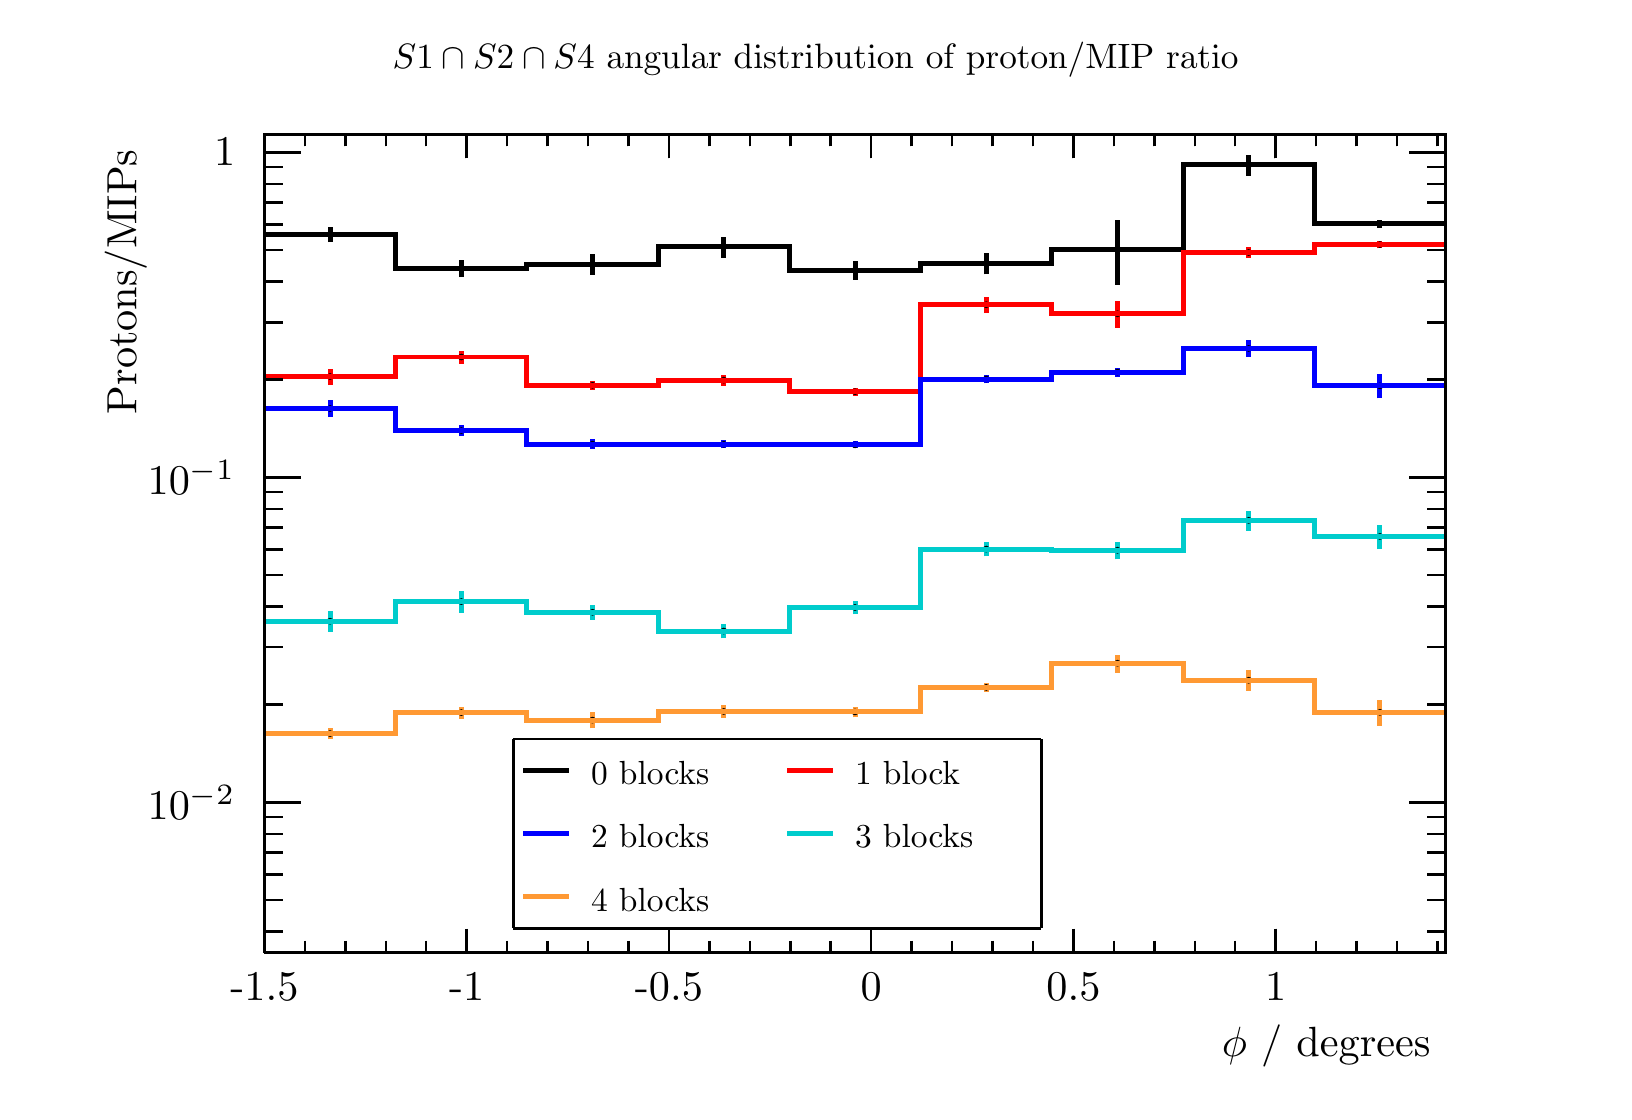
\begin{tikzpicture}
\pgfdeclareplotmark{cross} {
\pgfpathmoveto{\pgfpoint{-0.3\pgfplotmarksize}{\pgfplotmarksize}}
\pgfpathlineto{\pgfpoint{+0.3\pgfplotmarksize}{\pgfplotmarksize}}
\pgfpathlineto{\pgfpoint{+0.3\pgfplotmarksize}{0.3\pgfplotmarksize}}
\pgfpathlineto{\pgfpoint{+1\pgfplotmarksize}{0.3\pgfplotmarksize}}
\pgfpathlineto{\pgfpoint{+1\pgfplotmarksize}{-0.3\pgfplotmarksize}}
\pgfpathlineto{\pgfpoint{+0.3\pgfplotmarksize}{-0.3\pgfplotmarksize}}
\pgfpathlineto{\pgfpoint{+0.3\pgfplotmarksize}{-1.\pgfplotmarksize}}
\pgfpathlineto{\pgfpoint{-0.3\pgfplotmarksize}{-1.\pgfplotmarksize}}
\pgfpathlineto{\pgfpoint{-0.3\pgfplotmarksize}{-0.3\pgfplotmarksize}}
\pgfpathlineto{\pgfpoint{-1.\pgfplotmarksize}{-0.3\pgfplotmarksize}}
\pgfpathlineto{\pgfpoint{-1.\pgfplotmarksize}{0.3\pgfplotmarksize}}
\pgfpathlineto{\pgfpoint{-0.3\pgfplotmarksize}{0.3\pgfplotmarksize}}
\pgfpathclose
\pgfusepathqstroke
}
\pgfdeclareplotmark{cross*} {
\pgfpathmoveto{\pgfpoint{-0.3\pgfplotmarksize}{\pgfplotmarksize}}
\pgfpathlineto{\pgfpoint{+0.3\pgfplotmarksize}{\pgfplotmarksize}}
\pgfpathlineto{\pgfpoint{+0.3\pgfplotmarksize}{0.3\pgfplotmarksize}}
\pgfpathlineto{\pgfpoint{+1\pgfplotmarksize}{0.3\pgfplotmarksize}}
\pgfpathlineto{\pgfpoint{+1\pgfplotmarksize}{-0.3\pgfplotmarksize}}
\pgfpathlineto{\pgfpoint{+0.3\pgfplotmarksize}{-0.3\pgfplotmarksize}}
\pgfpathlineto{\pgfpoint{+0.3\pgfplotmarksize}{-1.\pgfplotmarksize}}
\pgfpathlineto{\pgfpoint{-0.3\pgfplotmarksize}{-1.\pgfplotmarksize}}
\pgfpathlineto{\pgfpoint{-0.3\pgfplotmarksize}{-0.3\pgfplotmarksize}}
\pgfpathlineto{\pgfpoint{-1.\pgfplotmarksize}{-0.3\pgfplotmarksize}}
\pgfpathlineto{\pgfpoint{-1.\pgfplotmarksize}{0.3\pgfplotmarksize}}
\pgfpathlineto{\pgfpoint{-0.3\pgfplotmarksize}{0.3\pgfplotmarksize}}
\pgfpathclose
\pgfusepathqfillstroke
}
\pgfdeclareplotmark{newstar} {
\pgfpathmoveto{\pgfqpoint{0pt}{\pgfplotmarksize}}
\pgfpathlineto{\pgfqpointpolar{44}{0.5\pgfplotmarksize}}
\pgfpathlineto{\pgfqpointpolar{18}{\pgfplotmarksize}}
\pgfpathlineto{\pgfqpointpolar{-20}{0.5\pgfplotmarksize}}
\pgfpathlineto{\pgfqpointpolar{-54}{\pgfplotmarksize}}
\pgfpathlineto{\pgfqpointpolar{-90}{0.5\pgfplotmarksize}}
\pgfpathlineto{\pgfqpointpolar{234}{\pgfplotmarksize}}
\pgfpathlineto{\pgfqpointpolar{198}{0.5\pgfplotmarksize}}
\pgfpathlineto{\pgfqpointpolar{162}{\pgfplotmarksize}}
\pgfpathlineto{\pgfqpointpolar{134}{0.5\pgfplotmarksize}}
\pgfpathclose
\pgfusepathqstroke
}
\pgfdeclareplotmark{newstar*} {
\pgfpathmoveto{\pgfqpoint{0pt}{\pgfplotmarksize}}
\pgfpathlineto{\pgfqpointpolar{44}{0.5\pgfplotmarksize}}
\pgfpathlineto{\pgfqpointpolar{18}{\pgfplotmarksize}}
\pgfpathlineto{\pgfqpointpolar{-20}{0.5\pgfplotmarksize}}
\pgfpathlineto{\pgfqpointpolar{-54}{\pgfplotmarksize}}
\pgfpathlineto{\pgfqpointpolar{-90}{0.5\pgfplotmarksize}}
\pgfpathlineto{\pgfqpointpolar{234}{\pgfplotmarksize}}
\pgfpathlineto{\pgfqpointpolar{198}{0.5\pgfplotmarksize}}
\pgfpathlineto{\pgfqpointpolar{162}{\pgfplotmarksize}}
\pgfpathlineto{\pgfqpointpolar{134}{0.5\pgfplotmarksize}}
\pgfpathclose
\pgfusepathqfillstroke
}
\definecolor{c}{rgb}{1,1,1};
\draw [color=c, fill=c] (0,0) rectangle (20,13.4957);
\draw [color=c, fill=c] (3,1.75444) rectangle (18,12.1461);
\definecolor{c}{rgb}{0,0,0};
\draw [c,line width=0.9] (3,1.75444) -- (3,12.1461) -- (18,12.1461) -- (18,1.75444) -- (3,1.75444);
\definecolor{c}{rgb}{1,1,1};
\draw [color=c, fill=c] (3,1.75444) rectangle (18,12.1461);
\definecolor{c}{rgb}{0,0,0};
\draw [c,line width=0.9] (3,1.75444) -- (3,12.1461) -- (18,12.1461) -- (18,1.75444) -- (3,1.75444);
\draw [c,line width=0.9] (3,1.75444) -- (4.66667,1.75444) -- (4.66667,1.75444) -- (6.33333,1.75444) -- (6.33333,1.75444) -- (8,1.75444) -- (8,1.75444) -- (9.66667,1.75444) -- (9.66667,1.75444) -- (11.3333,1.75444) -- (11.3333,1.75444) -- (13,1.75444)
 -- (13,1.75444) -- (14.6667,1.75444) -- (14.6667,1.75444) -- (16.3333,1.75444) -- (16.3333,1.75444) -- (18,1.75444);
\draw [c,line width=0.9] (3,1.75444) -- (18,1.75444);
\draw [c,line width=0.9] (3,2.05809) -- (3,1.75444);
\draw [c,line width=0.9] (3.5137,1.90627) -- (3.5137,1.75444);
\draw [c,line width=0.9] (4.0274,1.90627) -- (4.0274,1.75444);
\draw [c,line width=0.9] (4.5411,1.90627) -- (4.5411,1.75444);
\draw [c,line width=0.9] (5.05479,1.90627) -- (5.05479,1.75444);
\draw [c,line width=0.9] (5.56849,2.05809) -- (5.56849,1.75444);
\draw [c,line width=0.9] (6.08219,1.90627) -- (6.08219,1.75444);
\draw [c,line width=0.9] (6.59589,1.90627) -- (6.59589,1.75444);
\draw [c,line width=0.9] (7.10959,1.90627) -- (7.10959,1.75444);
\draw [c,line width=0.9] (7.62329,1.90627) -- (7.62329,1.75444);
\draw [c,line width=0.9] (8.13699,2.05809) -- (8.13699,1.75444);
\draw [c,line width=0.9] (8.65069,1.90627) -- (8.65069,1.75444);
\draw [c,line width=0.9] (9.16438,1.90627) -- (9.16438,1.75444);
\draw [c,line width=0.9] (9.67808,1.90627) -- (9.67808,1.75444);
\draw [c,line width=0.9] (10.1918,1.90627) -- (10.1918,1.75444);
\draw [c,line width=0.9] (10.7055,2.05809) -- (10.7055,1.75444);
\draw [c,line width=0.9] (11.2192,1.90627) -- (11.2192,1.75444);
\draw [c,line width=0.9] (11.7329,1.90627) -- (11.7329,1.75444);
\draw [c,line width=0.9] (12.2466,1.90627) -- (12.2466,1.75444);
\draw [c,line width=0.9] (12.7603,1.90627) -- (12.7603,1.75444);
\draw [c,line width=0.9] (13.274,2.05809) -- (13.274,1.75444);
\draw [c,line width=0.9] (13.7877,1.90627) -- (13.7877,1.75444);
\draw [c,line width=0.9] (14.3014,1.90627) -- (14.3014,1.75444);
\draw [c,line width=0.9] (14.8151,1.90627) -- (14.8151,1.75444);
\draw [c,line width=0.9] (15.3288,1.90627) -- (15.3288,1.75444);
\draw [c,line width=0.9] (15.8425,2.05809) -- (15.8425,1.75444);
\draw [c,line width=0.9] (15.8425,2.05809) -- (15.8425,1.75444);
\draw [c,line width=0.9] (16.3562,1.90627) -- (16.3562,1.75444);
\draw [c,line width=0.9] (16.8699,1.90627) -- (16.8699,1.75444);
\draw [c,line width=0.9] (17.3836,1.90627) -- (17.3836,1.75444);
\draw [c,line width=0.9] (17.8973,1.90627) -- (17.8973,1.75444);
\draw [anchor=base] (3,1.14713) node[scale=1.52731, color=c, rotate=0]{-1.5};
\draw [anchor=base] (5.56849,1.14713) node[scale=1.52731, color=c, rotate=0]{-1};
\draw [anchor=base] (8.13699,1.14713) node[scale=1.52731, color=c, rotate=0]{-0.5};
\draw [anchor=base] (10.7055,1.14713) node[scale=1.52731, color=c, rotate=0]{0};
\draw [anchor=base] (13.274,1.14713) node[scale=1.52731, color=c, rotate=0]{0.5};
\draw [anchor=base] (15.8425,1.14713) node[scale=1.52731, color=c, rotate=0]{1};
\draw [anchor= east] (18,0.566819) node[scale=1.52731, color=c, rotate=0]{$\phi$ / degrees};
\draw [c,line width=0.9] (3,12.1461) -- (18,12.1461);
\draw [c,line width=0.9] (3,11.8425) -- (3,12.1461);
\draw [c,line width=0.9] (3.5137,11.9943) -- (3.5137,12.1461);
\draw [c,line width=0.9] (4.0274,11.9943) -- (4.0274,12.1461);
\draw [c,line width=0.9] (4.5411,11.9943) -- (4.5411,12.1461);
\draw [c,line width=0.9] (5.05479,11.9943) -- (5.05479,12.1461);
\draw [c,line width=0.9] (5.56849,11.8425) -- (5.56849,12.1461);
\draw [c,line width=0.9] (6.08219,11.9943) -- (6.08219,12.1461);
\draw [c,line width=0.9] (6.59589,11.9943) -- (6.59589,12.1461);
\draw [c,line width=0.9] (7.10959,11.9943) -- (7.10959,12.1461);
\draw [c,line width=0.9] (7.62329,11.9943) -- (7.62329,12.1461);
\draw [c,line width=0.9] (8.13699,11.8425) -- (8.13699,12.1461);
\draw [c,line width=0.9] (8.65069,11.9943) -- (8.65069,12.1461);
\draw [c,line width=0.9] (9.16438,11.9943) -- (9.16438,12.1461);
\draw [c,line width=0.9] (9.67808,11.9943) -- (9.67808,12.1461);
\draw [c,line width=0.9] (10.1918,11.9943) -- (10.1918,12.1461);
\draw [c,line width=0.9] (10.7055,11.8425) -- (10.7055,12.1461);
\draw [c,line width=0.9] (11.2192,11.9943) -- (11.2192,12.1461);
\draw [c,line width=0.9] (11.7329,11.9943) -- (11.7329,12.1461);
\draw [c,line width=0.9] (12.2466,11.9943) -- (12.2466,12.1461);
\draw [c,line width=0.9] (12.7603,11.9943) -- (12.7603,12.1461);
\draw [c,line width=0.9] (13.274,11.8425) -- (13.274,12.1461);
\draw [c,line width=0.9] (13.7877,11.9943) -- (13.7877,12.1461);
\draw [c,line width=0.9] (14.3014,11.9943) -- (14.3014,12.1461);
\draw [c,line width=0.9] (14.8151,11.9943) -- (14.8151,12.1461);
\draw [c,line width=0.9] (15.3288,11.9943) -- (15.3288,12.1461);
\draw [c,line width=0.9] (15.8425,11.8425) -- (15.8425,12.1461);
\draw [c,line width=0.9] (15.8425,11.8425) -- (15.8425,12.1461);
\draw [c,line width=0.9] (16.3562,11.9943) -- (16.3562,12.1461);
\draw [c,line width=0.9] (16.8699,11.9943) -- (16.8699,12.1461);
\draw [c,line width=0.9] (17.3836,11.9943) -- (17.3836,12.1461);
\draw [c,line width=0.9] (17.8973,11.9943) -- (17.8973,12.1461);
\draw [c,line width=0.9] (3,1.75444) -- (3,12.1461);
\draw [c,line width=0.9] (3.231,2.0228) -- (3,2.0228);
\draw [c,line width=0.9] (3.231,2.42276) -- (3,2.42276);
\draw [c,line width=0.9] (3.231,2.74954) -- (3,2.74954);
\draw [c,line width=0.9] (3.231,3.02584) -- (3,3.02584);
\draw [c,line width=0.9] (3.231,3.26518) -- (3,3.26518);
\draw [c,line width=0.9] (3.231,3.47629) -- (3,3.47629);
\draw [c,line width=0.9] (3.462,3.66514) -- (3,3.66514);
\draw [anchor= east] (2.82,3.66514) node[scale=1.52731, color=c, rotate=0]{$10^{-2}$};
\draw [c,line width=0.9] (3.231,4.90752) -- (3,4.90752);
\draw [c,line width=0.9] (3.231,5.63427) -- (3,5.63427);
\draw [c,line width=0.9] (3.231,6.1499) -- (3,6.1499);
\draw [c,line width=0.9] (3.231,6.54986) -- (3,6.54986);
\draw [c,line width=0.9] (3.231,6.87665) -- (3,6.87665);
\draw [c,line width=0.9] (3.231,7.15295) -- (3,7.15295);
\draw [c,line width=0.9] (3.231,7.39229) -- (3,7.39229);
\draw [c,line width=0.9] (3.231,7.6034) -- (3,7.6034);
\draw [c,line width=0.9] (3.462,7.79224) -- (3,7.79224);
\draw [anchor= east] (2.82,7.79224) node[scale=1.52731, color=c, rotate=0]{$10^{-1}$};
\draw [c,line width=0.9] (3.231,9.03463) -- (3,9.03463);
\draw [c,line width=0.9] (3.231,9.76137) -- (3,9.76137);
\draw [c,line width=0.9] (3.231,10.277) -- (3,10.277);
\draw [c,line width=0.9] (3.231,10.677) -- (3,10.677);
\draw [c,line width=0.9] (3.231,11.0038) -- (3,11.0038);
\draw [c,line width=0.9] (3.231,11.2801) -- (3,11.2801);
\draw [c,line width=0.9] (3.231,11.5194) -- (3,11.5194);
\draw [c,line width=0.9] (3.231,11.7305) -- (3,11.7305);
\draw [c,line width=0.9] (3.462,11.9193) -- (3,11.9193);
\draw [anchor= east] (2.82,11.9193) node[scale=1.52731, color=c, rotate=0]{1};
\draw [anchor= east] (1.24,12.1461) node[scale=1.52731, color=c, rotate=90]{ Protons/MIPs};
\draw [c,line width=0.9] (18,1.75444) -- (18,12.1461);
\draw [c,line width=0.9] (17.769,2.0228) -- (18,2.0228);
\draw [c,line width=0.9] (17.769,2.42276) -- (18,2.42276);
\draw [c,line width=0.9] (17.769,2.74954) -- (18,2.74954);
\draw [c,line width=0.9] (17.769,3.02584) -- (18,3.02584);
\draw [c,line width=0.9] (17.769,3.26518) -- (18,3.26518);
\draw [c,line width=0.9] (17.769,3.47629) -- (18,3.47629);
\draw [c,line width=0.9] (17.538,3.66514) -- (18,3.66514);
\draw [c,line width=0.9] (17.769,4.90752) -- (18,4.90752);
\draw [c,line width=0.9] (17.769,5.63427) -- (18,5.63427);
\draw [c,line width=0.9] (17.769,6.1499) -- (18,6.1499);
\draw [c,line width=0.9] (17.769,6.54986) -- (18,6.54986);
\draw [c,line width=0.9] (17.769,6.87665) -- (18,6.87665);
\draw [c,line width=0.9] (17.769,7.15295) -- (18,7.15295);
\draw [c,line width=0.9] (17.769,7.39229) -- (18,7.39229);
\draw [c,line width=0.9] (17.769,7.6034) -- (18,7.6034);
\draw [c,line width=0.9] (17.538,7.79224) -- (18,7.79224);
\draw [c,line width=0.9] (17.769,9.03463) -- (18,9.03463);
\draw [c,line width=0.9] (17.769,9.76137) -- (18,9.76137);
\draw [c,line width=0.9] (17.769,10.277) -- (18,10.277);
\draw [c,line width=0.9] (17.769,10.677) -- (18,10.677);
\draw [c,line width=0.9] (17.769,11.0038) -- (18,11.0038);
\draw [c,line width=0.9] (17.769,11.2801) -- (18,11.2801);
\draw [c,line width=0.9] (17.769,11.5194) -- (18,11.5194);
\draw [c,line width=0.9] (17.769,11.7305) -- (18,11.7305);
\draw [c,line width=0.9] (17.538,11.9193) -- (18,11.9193);
\draw [c,line width=1.8] (3.83333,10.7777) -- (3.83333,10.8765);
\draw [c,line width=1.8] (3.83333,10.8765) -- (3.83333,10.9702);
\foreach \P in {(3.83333,10.8765)}{\draw[mark options={color=c,fill=c},mark size=2.402402pt,mark=*,mark size=1pt] plot coordinates {\P};}
\draw [c,line width=1.8] (5.5,10.3339) -- (5.5,10.4447);
\draw [c,line width=1.8] (5.5,10.4447) -- (5.5,10.549);
\foreach \P in {(5.5,10.4447)}{\draw[mark options={color=c,fill=c},mark size=2.402402pt,mark=*,mark size=1pt] plot coordinates {\P};}
\draw [c,line width=1.8] (7.16667,10.362) -- (7.16667,10.4971);
\draw [c,line width=1.8] (7.16667,10.4971) -- (7.16667,10.6227);
\foreach \P in {(7.16667,10.4971)}{\draw[mark options={color=c,fill=c},mark size=2.402402pt,mark=*,mark size=1pt] plot coordinates {\P};}
\draw [c,line width=1.8] (8.83333,10.5803) -- (8.83333,10.72);
\draw [c,line width=1.8] (8.83333,10.72) -- (8.83333,10.8497);
\foreach \P in {(8.83333,10.72)}{\draw[mark options={color=c,fill=c},mark size=2.402402pt,mark=*,mark size=1pt] plot coordinates {\P};}
\draw [c,line width=1.8] (10.5,10.2982) -- (10.5,10.4208);
\draw [c,line width=1.8] (10.5,10.4208) -- (10.5,10.5355);
\foreach \P in {(10.5,10.4208)}{\draw[mark options={color=c,fill=c},mark size=2.402402pt,mark=*,mark size=1pt] plot coordinates {\P};}
\draw [c,line width=1.8] (12.1667,10.371) -- (12.1667,10.5085);
\draw [c,line width=1.8] (12.1667,10.5085) -- (12.1667,10.6363);
\foreach \P in {(12.1667,10.5085)}{\draw[mark options={color=c,fill=c},mark size=2.402402pt,mark=*,mark size=1pt] plot coordinates {\P};}
\draw [c,line width=1.8] (13.8333,10.2369) -- (13.8333,10.6916);
\draw [c,line width=1.8] (13.8333,10.6916) -- (13.8333,11.054);
\foreach \P in {(13.8333,10.6916)}{\draw[mark options={color=c,fill=c},mark size=2.402402pt,mark=*,mark size=1pt] plot coordinates {\P};}
\draw [c,line width=1.8] (15.5,11.6218) -- (15.5,11.7605);
\draw [c,line width=1.8] (15.5,11.7605) -- (15.5,11.8893);
\foreach \P in {(15.5,11.7605)}{\draw[mark options={color=c,fill=c},mark size=2.402402pt,mark=*,mark size=1pt] plot coordinates {\P};}
\draw [c,line width=1.8] (17.1667,10.9639) -- (17.1667,11.0149);
\draw [c,line width=1.8] (17.1667,11.0149) -- (17.1667,11.0645);
\foreach \P in {(17.1667,11.0149)}{\draw[mark options={color=c,fill=c},mark size=2.402402pt,mark=*,mark size=1pt] plot coordinates {\P};}
\draw [c,line width=1.8] (3,10.8765) -- (4.66667,10.8765) -- (4.66667,10.4447) -- (6.33333,10.4447) -- (6.33333,10.4971) -- (8,10.4971) -- (8,10.72) -- (9.66667,10.72) -- (9.66667,10.4208) -- (11.3333,10.4208) -- (11.3333,10.5085) -- (13,10.5085) --
 (13,10.6916) -- (14.6667,10.6916) -- (14.6667,11.7605) -- (16.3333,11.7605) -- (16.3333,11.0149) -- (18,11.0149);
\definecolor{c}{rgb}{1,0,0};
\draw [c,line width=1.8] (3.83333,8.96432) -- (3.83333,9.07217);
\draw [c,line width=1.8] (3.83333,9.07217) -- (3.83333,9.17389);
\definecolor{c}{rgb}{0,0,0};
\foreach \P in {(3.83333,9.07217)}{\draw[mark options={color=c,fill=c},mark size=2.402402pt,mark=*,mark size=1pt] plot coordinates {\P};}
\definecolor{c}{rgb}{1,0,0};
\draw [c,line width=1.8] (5.5,9.23726) -- (5.5,9.32023);
\draw [c,line width=1.8] (5.5,9.32023) -- (5.5,9.39953);
\definecolor{c}{rgb}{0,0,0};
\foreach \P in {(5.5,9.32023)}{\draw[mark options={color=c,fill=c},mark size=2.402402pt,mark=*,mark size=1pt] plot coordinates {\P};}
\definecolor{c}{rgb}{1,0,0};
\draw [c,line width=1.8] (7.16667,8.90343) -- (7.16667,8.96069);
\draw [c,line width=1.8] (7.16667,8.96069) -- (7.16667,9.01617);
\definecolor{c}{rgb}{0,0,0};
\foreach \P in {(7.16667,8.96069)}{\draw[mark options={color=c,fill=c},mark size=2.402402pt,mark=*,mark size=1pt] plot coordinates {\P};}
\definecolor{c}{rgb}{1,0,0};
\draw [c,line width=1.8] (8.83333,8.95669) -- (8.83333,9.02674);
\draw [c,line width=1.8] (8.83333,9.02674) -- (8.83333,9.09415);
\definecolor{c}{rgb}{0,0,0};
\foreach \P in {(8.83333,9.02674)}{\draw[mark options={color=c,fill=c},mark size=2.402402pt,mark=*,mark size=1pt] plot coordinates {\P};}
\definecolor{c}{rgb}{1,0,0};
\draw [c,line width=1.8] (10.5,8.82806) -- (10.5,8.87953);
\draw [c,line width=1.8] (10.5,8.87953) -- (10.5,8.92957);
\definecolor{c}{rgb}{0,0,0};
\foreach \P in {(10.5,8.87953)}{\draw[mark options={color=c,fill=c},mark size=2.402402pt,mark=*,mark size=1pt] plot coordinates {\P};}
\definecolor{c}{rgb}{1,0,0};
\draw [c,line width=1.8] (12.1667,9.87581) -- (12.1667,9.98442);
\draw [c,line width=1.8] (12.1667,9.98442) -- (12.1667,10.0868);
\definecolor{c}{rgb}{0,0,0};
\foreach \P in {(12.1667,9.98442)}{\draw[mark options={color=c,fill=c},mark size=2.402402pt,mark=*,mark size=1pt] plot coordinates {\P};}
\definecolor{c}{rgb}{1,0,0};
\draw [c,line width=1.8] (13.8333,9.69229) -- (13.8333,9.86902);
\draw [c,line width=1.8] (13.8333,9.86902) -- (13.8333,10.0299);
\definecolor{c}{rgb}{0,0,0};
\foreach \P in {(13.8333,9.86902)}{\draw[mark options={color=c,fill=c},mark size=2.402402pt,mark=*,mark size=1pt] plot coordinates {\P};}
\definecolor{c}{rgb}{1,0,0};
\draw [c,line width=1.8] (15.5,10.576) -- (15.5,10.6472);
\draw [c,line width=1.8] (15.5,10.6472) -- (15.5,10.7157);
\definecolor{c}{rgb}{0,0,0};
\foreach \P in {(15.5,10.6472)}{\draw[mark options={color=c,fill=c},mark size=2.402402pt,mark=*,mark size=1pt] plot coordinates {\P};}
\definecolor{c}{rgb}{1,0,0};
\draw [c,line width=1.8] (17.1667,10.6997) -- (17.1667,10.7481);
\draw [c,line width=1.8] (17.1667,10.7481) -- (17.1667,10.7953);
\definecolor{c}{rgb}{0,0,0};
\foreach \P in {(17.1667,10.7481)}{\draw[mark options={color=c,fill=c},mark size=2.402402pt,mark=*,mark size=1pt] plot coordinates {\P};}
\definecolor{c}{rgb}{1,0,0};
\draw [c,line width=1.8] (3,9.07217) -- (4.66667,9.07217) -- (4.66667,9.32023) -- (6.33333,9.32023) -- (6.33333,8.96069) -- (8,8.96069) -- (8,9.02674) -- (9.66667,9.02674) -- (9.66667,8.87953) -- (11.3333,8.87953) -- (11.3333,9.98442) -- (13,9.98442)
 -- (13,9.86902) -- (14.6667,9.86902) -- (14.6667,10.6472) -- (16.3333,10.6472) -- (16.3333,10.7481) -- (18,10.7481);
\definecolor{c}{rgb}{0,0,1};
\draw [c,line width=1.8] (3.83333,8.55718) -- (3.83333,8.66636);
\draw [c,line width=1.8] (3.83333,8.66636) -- (3.83333,8.76928);
\definecolor{c}{rgb}{0,0,0};
\foreach \P in {(3.83333,8.66636)}{\draw[mark options={color=c,fill=c},mark size=2.402402pt,mark=*,mark size=1pt] plot coordinates {\P};}
\definecolor{c}{rgb}{0,0,1};
\draw [c,line width=1.8] (5.5,8.31557) -- (5.5,8.38631);
\draw [c,line width=1.8] (5.5,8.38631) -- (5.5,8.45436);
\definecolor{c}{rgb}{0,0,0};
\foreach \P in {(5.5,8.38631)}{\draw[mark options={color=c,fill=c},mark size=2.402402pt,mark=*,mark size=1pt] plot coordinates {\P};}
\definecolor{c}{rgb}{0,0,1};
\draw [c,line width=1.8] (7.16667,8.15197) -- (7.16667,8.21352);
\draw [c,line width=1.8] (7.16667,8.21352) -- (7.16667,8.27302);
\definecolor{c}{rgb}{0,0,0};
\foreach \P in {(7.16667,8.21352)}{\draw[mark options={color=c,fill=c},mark size=2.402402pt,mark=*,mark size=1pt] plot coordinates {\P};}
\definecolor{c}{rgb}{0,0,1};
\draw [c,line width=1.8] (8.83333,8.15946) -- (8.83333,8.21131);
\draw [c,line width=1.8] (8.83333,8.21131) -- (8.83333,8.26171);
\definecolor{c}{rgb}{0,0,0};
\foreach \P in {(8.83333,8.21131)}{\draw[mark options={color=c,fill=c},mark size=2.402402pt,mark=*,mark size=1pt] plot coordinates {\P};}
\definecolor{c}{rgb}{0,0,1};
\draw [c,line width=1.8] (10.5,8.15949) -- (10.5,8.20403);
\draw [c,line width=1.8] (10.5,8.20403) -- (10.5,8.24749);
\definecolor{c}{rgb}{0,0,0};
\foreach \P in {(10.5,8.20403)}{\draw[mark options={color=c,fill=c},mark size=2.402402pt,mark=*,mark size=1pt] plot coordinates {\P};}
\definecolor{c}{rgb}{0,0,1};
\draw [c,line width=1.8] (12.1667,8.98631) -- (12.1667,9.04063);
\draw [c,line width=1.8] (12.1667,9.04063) -- (12.1667,9.09336);
\definecolor{c}{rgb}{0,0,0};
\foreach \P in {(12.1667,9.04063)}{\draw[mark options={color=c,fill=c},mark size=2.402402pt,mark=*,mark size=1pt] plot coordinates {\P};}
\definecolor{c}{rgb}{0,0,1};
\draw [c,line width=1.8] (13.8333,9.07201) -- (13.8333,9.12799);
\draw [c,line width=1.8] (13.8333,9.12799) -- (13.8333,9.18227);
\definecolor{c}{rgb}{0,0,0};
\foreach \P in {(13.8333,9.12799)}{\draw[mark options={color=c,fill=c},mark size=2.402402pt,mark=*,mark size=1pt] plot coordinates {\P};}
\definecolor{c}{rgb}{0,0,1};
\draw [c,line width=1.8] (15.5,9.32044) -- (15.5,9.42921);
\draw [c,line width=1.8] (15.5,9.42921) -- (15.5,9.53176);
\definecolor{c}{rgb}{0,0,0};
\foreach \P in {(15.5,9.42921)}{\draw[mark options={color=c,fill=c},mark size=2.402402pt,mark=*,mark size=1pt] plot coordinates {\P};}
\definecolor{c}{rgb}{0,0,1};
\draw [c,line width=1.8] (17.1667,8.79549) -- (17.1667,8.95348);
\draw [c,line width=1.8] (17.1667,8.95348) -- (17.1667,9.09867);
\definecolor{c}{rgb}{0,0,0};
\foreach \P in {(17.1667,8.95348)}{\draw[mark options={color=c,fill=c},mark size=2.402402pt,mark=*,mark size=1pt] plot coordinates {\P};}
\definecolor{c}{rgb}{0,0,1};
\draw [c,line width=1.8] (3,8.66636) -- (4.66667,8.66636) -- (4.66667,8.38631) -- (6.33333,8.38631) -- (6.33333,8.21352) -- (8,8.21352) -- (8,8.21131) -- (9.66667,8.21131) -- (9.66667,8.20403) -- (11.3333,8.20403) -- (11.3333,9.04063) -- (13,9.04063)
 -- (13,9.12799) -- (14.6667,9.12799) -- (14.6667,9.42921) -- (16.3333,9.42921) -- (16.3333,8.95348) -- (18,8.95348);
\definecolor{c}{rgb}{0,0.8,0.8};
\draw [c,line width=1.8] (3.83333,5.82959) -- (3.83333,5.9648);
\draw [c,line width=1.8] (3.83333,5.9648) -- (3.83333,6.09053);
\definecolor{c}{rgb}{0,0,0};
\foreach \P in {(3.83333,5.9648)}{\draw[mark options={color=c,fill=c},mark size=2.402402pt,mark=*,mark size=1pt] plot coordinates {\P};}
\definecolor{c}{rgb}{0,0.8,0.8};
\draw [c,line width=1.8] (5.5,6.07356) -- (5.5,6.21409);
\draw [c,line width=1.8] (5.5,6.21409) -- (5.5,6.3444);
\definecolor{c}{rgb}{0,0,0};
\foreach \P in {(5.5,6.21409)}{\draw[mark options={color=c,fill=c},mark size=2.402402pt,mark=*,mark size=1pt] plot coordinates {\P};}
\definecolor{c}{rgb}{0,0.8,0.8};
\draw [c,line width=1.8] (7.16667,5.98519) -- (7.16667,6.07802);
\draw [c,line width=1.8] (7.16667,6.07802) -- (7.16667,6.16629);
\definecolor{c}{rgb}{0,0,0};
\foreach \P in {(7.16667,6.07802)}{\draw[mark options={color=c,fill=c},mark size=2.402402pt,mark=*,mark size=1pt] plot coordinates {\P};}
\definecolor{c}{rgb}{0,0.8,0.8};
\draw [c,line width=1.8] (8.83333,5.7463) -- (8.83333,5.84009);
\draw [c,line width=1.8] (8.83333,5.84009) -- (8.83333,5.92921);
\definecolor{c}{rgb}{0,0,0};
\foreach \P in {(8.83333,5.84009)}{\draw[mark options={color=c,fill=c},mark size=2.402402pt,mark=*,mark size=1pt] plot coordinates {\P};}
\definecolor{c}{rgb}{0,0.8,0.8};
\draw [c,line width=1.8] (10.5,6.05372) -- (10.5,6.13878);
\draw [c,line width=1.8] (10.5,6.13878) -- (10.5,6.21999);
\definecolor{c}{rgb}{0,0,0};
\foreach \P in {(10.5,6.13878)}{\draw[mark options={color=c,fill=c},mark size=2.402402pt,mark=*,mark size=1pt] plot coordinates {\P};}
\definecolor{c}{rgb}{0,0.8,0.8};
\draw [c,line width=1.8] (12.1667,6.78835) -- (12.1667,6.88104);
\draw [c,line width=1.8] (12.1667,6.88104) -- (12.1667,6.96918);
\definecolor{c}{rgb}{0,0,0};
\foreach \P in {(12.1667,6.88104)}{\draw[mark options={color=c,fill=c},mark size=2.402402pt,mark=*,mark size=1pt] plot coordinates {\P};}
\definecolor{c}{rgb}{0,0.8,0.8};
\draw [c,line width=1.8] (13.8333,6.75097) -- (13.8333,6.86591);
\draw [c,line width=1.8] (13.8333,6.86591) -- (13.8333,6.97393);
\definecolor{c}{rgb}{0,0,0};
\foreach \P in {(13.8333,6.86591)}{\draw[mark options={color=c,fill=c},mark size=2.402402pt,mark=*,mark size=1pt] plot coordinates {\P};}
\definecolor{c}{rgb}{0,0.8,0.8};
\draw [c,line width=1.8] (15.5,7.11167) -- (15.5,7.24588);
\draw [c,line width=1.8] (15.5,7.24588) -- (15.5,7.37073);
\definecolor{c}{rgb}{0,0,0};
\foreach \P in {(15.5,7.24588)}{\draw[mark options={color=c,fill=c},mark size=2.402402pt,mark=*,mark size=1pt] plot coordinates {\P};}
\definecolor{c}{rgb}{0,0.8,0.8};
\draw [c,line width=1.8] (17.1667,6.88029) -- (17.1667,7.0412);
\draw [c,line width=1.8] (17.1667,7.0412) -- (17.1667,7.18884);
\definecolor{c}{rgb}{0,0,0};
\foreach \P in {(17.1667,7.0412)}{\draw[mark options={color=c,fill=c},mark size=2.402402pt,mark=*,mark size=1pt] plot coordinates {\P};}
\definecolor{c}{rgb}{0,0.8,0.8};
\draw [c,line width=1.8] (3,5.9648) -- (4.66667,5.9648) -- (4.66667,6.21409) -- (6.33333,6.21409) -- (6.33333,6.07802) -- (8,6.07802) -- (8,5.84009) -- (9.66667,5.84009) -- (9.66667,6.13878) -- (11.3333,6.13878) -- (11.3333,6.88104) -- (13,6.88104)
 -- (13,6.86591) -- (14.6667,6.86591) -- (14.6667,7.24588) -- (16.3333,7.24588) -- (16.3333,7.0412) -- (18,7.0412);
\definecolor{c}{rgb}{1,0.6,0.2};
\draw [c,line width=1.8] (3.83333,4.46453) -- (3.83333,4.53759);
\draw [c,line width=1.8] (3.83333,4.53759) -- (3.83333,4.60778);
\definecolor{c}{rgb}{0,0,0};
\foreach \P in {(3.83333,4.53759)}{\draw[mark options={color=c,fill=c},mark size=2.402402pt,mark=*,mark size=1pt] plot coordinates {\P};}
\definecolor{c}{rgb}{1,0.6,0.2};
\draw [c,line width=1.8] (5.5,4.72766) -- (5.5,4.80432);
\draw [c,line width=1.8] (5.5,4.80432) -- (5.5,4.87783);
\definecolor{c}{rgb}{0,0,0};
\foreach \P in {(5.5,4.80432)}{\draw[mark options={color=c,fill=c},mark size=2.402402pt,mark=*,mark size=1pt] plot coordinates {\P};}
\definecolor{c}{rgb}{1,0.6,0.2};
\draw [c,line width=1.8] (7.16667,4.60307) -- (7.16667,4.70869);
\draw [c,line width=1.8] (7.16667,4.70869) -- (7.16667,4.80844);
\definecolor{c}{rgb}{0,0,0};
\foreach \P in {(7.16667,4.70869)}{\draw[mark options={color=c,fill=c},mark size=2.402402pt,mark=*,mark size=1pt] plot coordinates {\P};}
\definecolor{c}{rgb}{1,0.6,0.2};
\draw [c,line width=1.8] (8.83333,4.73762) -- (8.83333,4.81865);
\draw [c,line width=1.8] (8.83333,4.81865) -- (8.83333,4.89617);
\definecolor{c}{rgb}{0,0,0};
\foreach \P in {(8.83333,4.81865)}{\draw[mark options={color=c,fill=c},mark size=2.402402pt,mark=*,mark size=1pt] plot coordinates {\P};}
\definecolor{c}{rgb}{1,0.6,0.2};
\draw [c,line width=1.8] (10.5,4.74334) -- (10.5,4.81257);
\draw [c,line width=1.8] (10.5,4.81257) -- (10.5,4.87921);
\definecolor{c}{rgb}{0,0,0};
\foreach \P in {(10.5,4.81257)}{\draw[mark options={color=c,fill=c},mark size=2.402402pt,mark=*,mark size=1pt] plot coordinates {\P};}
\definecolor{c}{rgb}{1,0.6,0.2};
\draw [c,line width=1.8] (12.1667,5.06735) -- (12.1667,5.12404);
\draw [c,line width=1.8] (12.1667,5.12404) -- (12.1667,5.17899);
\definecolor{c}{rgb}{0,0,0};
\foreach \P in {(12.1667,5.12404)}{\draw[mark options={color=c,fill=c},mark size=2.402402pt,mark=*,mark size=1pt] plot coordinates {\P};}
\definecolor{c}{rgb}{1,0.6,0.2};
\draw [c,line width=1.8] (13.8333,5.31318) -- (13.8333,5.43116);
\draw [c,line width=1.8] (13.8333,5.43116) -- (13.8333,5.54185);
\definecolor{c}{rgb}{0,0,0};
\foreach \P in {(13.8333,5.43116)}{\draw[mark options={color=c,fill=c},mark size=2.402402pt,mark=*,mark size=1pt] plot coordinates {\P};}
\definecolor{c}{rgb}{1,0.6,0.2};
\draw [c,line width=1.8] (15.5,5.08173) -- (15.5,5.2152);
\draw [c,line width=1.8] (15.5,5.2152) -- (15.5,5.33942);
\definecolor{c}{rgb}{0,0,0};
\foreach \P in {(15.5,5.2152)}{\draw[mark options={color=c,fill=c},mark size=2.402402pt,mark=*,mark size=1pt] plot coordinates {\P};}
\definecolor{c}{rgb}{1,0.6,0.2};
\draw [c,line width=1.8] (17.1667,4.63598) -- (17.1667,4.80753);
\draw [c,line width=1.8] (17.1667,4.80753) -- (17.1667,4.96408);
\definecolor{c}{rgb}{0,0,0};
\foreach \P in {(17.1667,4.80753)}{\draw[mark options={color=c,fill=c},mark size=2.402402pt,mark=*,mark size=1pt] plot coordinates {\P};}
\definecolor{c}{rgb}{1,0.6,0.2};
\draw [c,line width=1.8] (3,4.53759) -- (4.66667,4.53759) -- (4.66667,4.80432) -- (6.33333,4.80432) -- (6.33333,4.70869) -- (8,4.70869) -- (8,4.81865) -- (9.66667,4.81865) -- (9.66667,4.81257) -- (11.3333,4.81257) -- (11.3333,5.12404) -- (13,5.12404)
 -- (13,5.43116) -- (14.6667,5.43116) -- (14.6667,5.2152) -- (16.3333,5.2152) -- (16.3333,4.80753) -- (18,4.80753);
\definecolor{c}{rgb}{0,0,0};
\draw [c,line width=0.9] (3,1.75444) -- (18,1.75444);
\draw [c,line width=0.9] (3,2.05809) -- (3,1.75444);
\draw [c,line width=0.9] (3.5137,1.90627) -- (3.5137,1.75444);
\draw [c,line width=0.9] (4.0274,1.90627) -- (4.0274,1.75444);
\draw [c,line width=0.9] (4.5411,1.90627) -- (4.5411,1.75444);
\draw [c,line width=0.9] (5.05479,1.90627) -- (5.05479,1.75444);
\draw [c,line width=0.9] (5.56849,2.05809) -- (5.56849,1.75444);
\draw [c,line width=0.9] (6.08219,1.90627) -- (6.08219,1.75444);
\draw [c,line width=0.9] (6.59589,1.90627) -- (6.59589,1.75444);
\draw [c,line width=0.9] (7.10959,1.90627) -- (7.10959,1.75444);
\draw [c,line width=0.9] (7.62329,1.90627) -- (7.62329,1.75444);
\draw [c,line width=0.9] (8.13699,2.05809) -- (8.13699,1.75444);
\draw [c,line width=0.9] (8.65069,1.90627) -- (8.65069,1.75444);
\draw [c,line width=0.9] (9.16438,1.90627) -- (9.16438,1.75444);
\draw [c,line width=0.9] (9.67808,1.90627) -- (9.67808,1.75444);
\draw [c,line width=0.9] (10.1918,1.90627) -- (10.1918,1.75444);
\draw [c,line width=0.9] (10.7055,2.05809) -- (10.7055,1.75444);
\draw [c,line width=0.9] (11.2192,1.90627) -- (11.2192,1.75444);
\draw [c,line width=0.9] (11.7329,1.90627) -- (11.7329,1.75444);
\draw [c,line width=0.9] (12.2466,1.90627) -- (12.2466,1.75444);
\draw [c,line width=0.9] (12.7603,1.90627) -- (12.7603,1.75444);
\draw [c,line width=0.9] (13.274,2.05809) -- (13.274,1.75444);
\draw [c,line width=0.9] (13.7877,1.90627) -- (13.7877,1.75444);
\draw [c,line width=0.9] (14.3014,1.90627) -- (14.3014,1.75444);
\draw [c,line width=0.9] (14.8151,1.90627) -- (14.8151,1.75444);
\draw [c,line width=0.9] (15.3288,1.90627) -- (15.3288,1.75444);
\draw [c,line width=0.9] (15.8425,2.05809) -- (15.8425,1.75444);
\draw [c,line width=0.9] (15.8425,2.05809) -- (15.8425,1.75444);
\draw [c,line width=0.9] (16.3562,1.90627) -- (16.3562,1.75444);
\draw [c,line width=0.9] (16.8699,1.90627) -- (16.8699,1.75444);
\draw [c,line width=0.9] (17.3836,1.90627) -- (17.3836,1.75444);
\draw [c,line width=0.9] (17.8973,1.90627) -- (17.8973,1.75444);
\draw [c,line width=0.9] (3,12.1461) -- (18,12.1461);
\draw [c,line width=0.9] (3,11.8425) -- (3,12.1461);
\draw [c,line width=0.9] (3.5137,11.9943) -- (3.5137,12.1461);
\draw [c,line width=0.9] (4.0274,11.9943) -- (4.0274,12.1461);
\draw [c,line width=0.9] (4.5411,11.9943) -- (4.5411,12.1461);
\draw [c,line width=0.9] (5.05479,11.9943) -- (5.05479,12.1461);
\draw [c,line width=0.9] (5.56849,11.8425) -- (5.56849,12.1461);
\draw [c,line width=0.9] (6.08219,11.9943) -- (6.08219,12.1461);
\draw [c,line width=0.9] (6.59589,11.9943) -- (6.59589,12.1461);
\draw [c,line width=0.9] (7.10959,11.9943) -- (7.10959,12.1461);
\draw [c,line width=0.9] (7.62329,11.9943) -- (7.62329,12.1461);
\draw [c,line width=0.9] (8.13699,11.8425) -- (8.13699,12.1461);
\draw [c,line width=0.9] (8.65069,11.9943) -- (8.65069,12.1461);
\draw [c,line width=0.9] (9.16438,11.9943) -- (9.16438,12.1461);
\draw [c,line width=0.9] (9.67808,11.9943) -- (9.67808,12.1461);
\draw [c,line width=0.9] (10.1918,11.9943) -- (10.1918,12.1461);
\draw [c,line width=0.9] (10.7055,11.8425) -- (10.7055,12.1461);
\draw [c,line width=0.9] (11.2192,11.9943) -- (11.2192,12.1461);
\draw [c,line width=0.9] (11.7329,11.9943) -- (11.7329,12.1461);
\draw [c,line width=0.9] (12.2466,11.9943) -- (12.2466,12.1461);
\draw [c,line width=0.9] (12.7603,11.9943) -- (12.7603,12.1461);
\draw [c,line width=0.9] (13.274,11.8425) -- (13.274,12.1461);
\draw [c,line width=0.9] (13.7877,11.9943) -- (13.7877,12.1461);
\draw [c,line width=0.9] (14.3014,11.9943) -- (14.3014,12.1461);
\draw [c,line width=0.9] (14.8151,11.9943) -- (14.8151,12.1461);
\draw [c,line width=0.9] (15.3288,11.9943) -- (15.3288,12.1461);
\draw [c,line width=0.9] (15.8425,11.8425) -- (15.8425,12.1461);
\draw [c,line width=0.9] (15.8425,11.8425) -- (15.8425,12.1461);
\draw [c,line width=0.9] (16.3562,11.9943) -- (16.3562,12.1461);
\draw [c,line width=0.9] (16.8699,11.9943) -- (16.8699,12.1461);
\draw [c,line width=0.9] (17.3836,11.9943) -- (17.3836,12.1461);
\draw [c,line width=0.9] (17.8973,11.9943) -- (17.8973,12.1461);
\draw [c,line width=0.9] (3,1.75444) -- (3,12.1461);
\draw [c,line width=0.9] (3.231,2.0228) -- (3,2.0228);
\draw [c,line width=0.9] (3.231,2.42276) -- (3,2.42276);
\draw [c,line width=0.9] (3.231,2.74954) -- (3,2.74954);
\draw [c,line width=0.9] (3.231,3.02584) -- (3,3.02584);
\draw [c,line width=0.9] (3.231,3.26518) -- (3,3.26518);
\draw [c,line width=0.9] (3.231,3.47629) -- (3,3.47629);
\draw [c,line width=0.9] (3.462,3.66514) -- (3,3.66514);
\draw [c,line width=0.9] (3.231,4.90752) -- (3,4.90752);
\draw [c,line width=0.9] (3.231,5.63427) -- (3,5.63427);
\draw [c,line width=0.9] (3.231,6.1499) -- (3,6.1499);
\draw [c,line width=0.9] (3.231,6.54986) -- (3,6.54986);
\draw [c,line width=0.9] (3.231,6.87665) -- (3,6.87665);
\draw [c,line width=0.9] (3.231,7.15295) -- (3,7.15295);
\draw [c,line width=0.9] (3.231,7.39229) -- (3,7.39229);
\draw [c,line width=0.9] (3.231,7.6034) -- (3,7.6034);
\draw [c,line width=0.9] (3.462,7.79224) -- (3,7.79224);
\draw [c,line width=0.9] (3.231,9.03463) -- (3,9.03463);
\draw [c,line width=0.9] (3.231,9.76137) -- (3,9.76137);
\draw [c,line width=0.9] (3.231,10.277) -- (3,10.277);
\draw [c,line width=0.9] (3.231,10.677) -- (3,10.677);
\draw [c,line width=0.9] (3.231,11.0038) -- (3,11.0038);
\draw [c,line width=0.9] (3.231,11.2801) -- (3,11.2801);
\draw [c,line width=0.9] (3.231,11.5194) -- (3,11.5194);
\draw [c,line width=0.9] (3.231,11.7305) -- (3,11.7305);
\draw [c,line width=0.9] (3.462,11.9193) -- (3,11.9193);
\draw [c,line width=0.9] (18,1.75444) -- (18,12.1461);
\draw [c,line width=0.9] (17.769,2.0228) -- (18,2.0228);
\draw [c,line width=0.9] (17.769,2.42276) -- (18,2.42276);
\draw [c,line width=0.9] (17.769,2.74954) -- (18,2.74954);
\draw [c,line width=0.9] (17.769,3.02584) -- (18,3.02584);
\draw [c,line width=0.9] (17.769,3.26518) -- (18,3.26518);
\draw [c,line width=0.9] (17.769,3.47629) -- (18,3.47629);
\draw [c,line width=0.9] (17.538,3.66514) -- (18,3.66514);
\draw [c,line width=0.9] (17.769,4.90752) -- (18,4.90752);
\draw [c,line width=0.9] (17.769,5.63427) -- (18,5.63427);
\draw [c,line width=0.9] (17.769,6.1499) -- (18,6.1499);
\draw [c,line width=0.9] (17.769,6.54986) -- (18,6.54986);
\draw [c,line width=0.9] (17.769,6.87665) -- (18,6.87665);
\draw [c,line width=0.9] (17.769,7.15295) -- (18,7.15295);
\draw [c,line width=0.9] (17.769,7.39229) -- (18,7.39229);
\draw [c,line width=0.9] (17.769,7.6034) -- (18,7.6034);
\draw [c,line width=0.9] (17.538,7.79224) -- (18,7.79224);
\draw [c,line width=0.9] (17.769,9.03463) -- (18,9.03463);
\draw [c,line width=0.9] (17.769,9.76137) -- (18,9.76137);
\draw [c,line width=0.9] (17.769,10.277) -- (18,10.277);
\draw [c,line width=0.9] (17.769,10.677) -- (18,10.677);
\draw [c,line width=0.9] (17.769,11.0038) -- (18,11.0038);
\draw [c,line width=0.9] (17.769,11.2801) -- (18,11.2801);
\draw [c,line width=0.9] (17.769,11.5194) -- (18,11.5194);
\draw [c,line width=0.9] (17.769,11.7305) -- (18,11.7305);
\draw [c,line width=0.9] (17.538,11.9193) -- (18,11.9193);
\definecolor{c}{rgb}{1,1,1};
\draw [color=c, fill=c] (2,12.7534) rectangle (18,13.4282);
\definecolor{c}{rgb}{0,0,0};
\draw (10,13.0908) node[scale=1.27276, color=c, rotate=0]{$S1 \cap S2 \cap S4$ angular distribution of proton/MIP ratio};
\definecolor{c}{rgb}{1,1,1};
\draw [color=c, fill=c] (6.16046,2.06304) rectangle (12.8653,4.46991);
\definecolor{c}{rgb}{0,0,0};
\draw [c,line width=0.9] (6.16046,2.06304) -- (12.8653,2.06304);
\draw [c,line width=0.9] (12.8653,2.06304) -- (12.8653,4.46991);
\draw [c,line width=0.9] (12.8653,4.46991) -- (6.16046,4.46991);
\draw [c,line width=0.9] (6.16046,4.46991) -- (6.16046,2.06304);
\draw [anchor=base west] (6.99857,3.88825) node[scale=1.20912, color=c, rotate=0]{0 blocks};
\draw [c,line width=1.8] (6.28617,4.06877) -- (6.87285,4.06877);
\draw [anchor=base west] (10.351,3.88825) node[scale=1.20912, color=c, rotate=0]{1 block};
\definecolor{c}{rgb}{1,0,0};
\draw [c,line width=1.8] (9.63861,4.06877) -- (10.2253,4.06877);
\definecolor{c}{rgb}{0,0,0};
\draw [anchor=base west] (6.99857,3.08596) node[scale=1.20912, color=c, rotate=0]{2 blocks};
\definecolor{c}{rgb}{0,0,1};
\draw [c,line width=1.8] (6.28617,3.26648) -- (6.87285,3.26648);
\definecolor{c}{rgb}{0,0,0};
\draw [anchor=base west] (10.351,3.08596) node[scale=1.20912, color=c, rotate=0]{3 blocks};
\definecolor{c}{rgb}{0,0.8,0.8};
\draw [c,line width=1.8] (9.63861,3.26648) -- (10.2253,3.26648);
\definecolor{c}{rgb}{0,0,0};
\draw [anchor=base west] (6.99857,2.28367) node[scale=1.20912, color=c, rotate=0]{4 blocks};
\definecolor{c}{rgb}{1,0.6,0.2};
\draw [c,line width=1.8] (6.28617,2.46418) -- (6.87285,2.46418);
\end{tikzpicture}

    \end{adjustbox}
    \caption{Proton-MIP ratio in $\mathit{S4}$ for varying numbers of moderator blocks as a function of vertical off-axis angle, as measured from $\mathit{S1}$.}
    \label{fig:propiratio_s4_vert}
  \end{minipage}	
\end{figure}

\subsection{Flux normalisation between detectors}

Because the portion of the beam subtended by each ToF detector is different, comparisons of the fluxes of various particles between detectors require the application of a normalisation.
\todo[inline]{JOCELYN: awkward. rephrase.}
These normalisations account both for solid angle coverage differences, and the different flux intensities present in the detectors.
Normalisation factors for comparing the flux are calculated and shown in table~\ref{tab:fluxFactors}.
These factors are calculated relative to the flux passing through $\mathit{S3}$ which covered the greatest angular extent of any of the timing points. 
The angular positions of the various timing points are shown in figure~\ref{fig:beamAng}.

\begin{figure}[h]
  
\end{figure}

The total flux passing through $\mathit{S1}$ and $\mathit{S3}$ is shown in figure~\ref{fig:s1s3all}.
This flux is normalised such that its area is equal to 1.
The factors are calculated by integrating this distribution between the angular limits of the other timing points.
Table~\ref{tab:fluxFactors} shows the calculated factors for various timing points and overlaps.

\begin{figure}[h]
  \begin{minipage}{0.49\textwidth}
    \begin{adjustbox}{max totalsize={\textwidth}{.5\textheight}}
      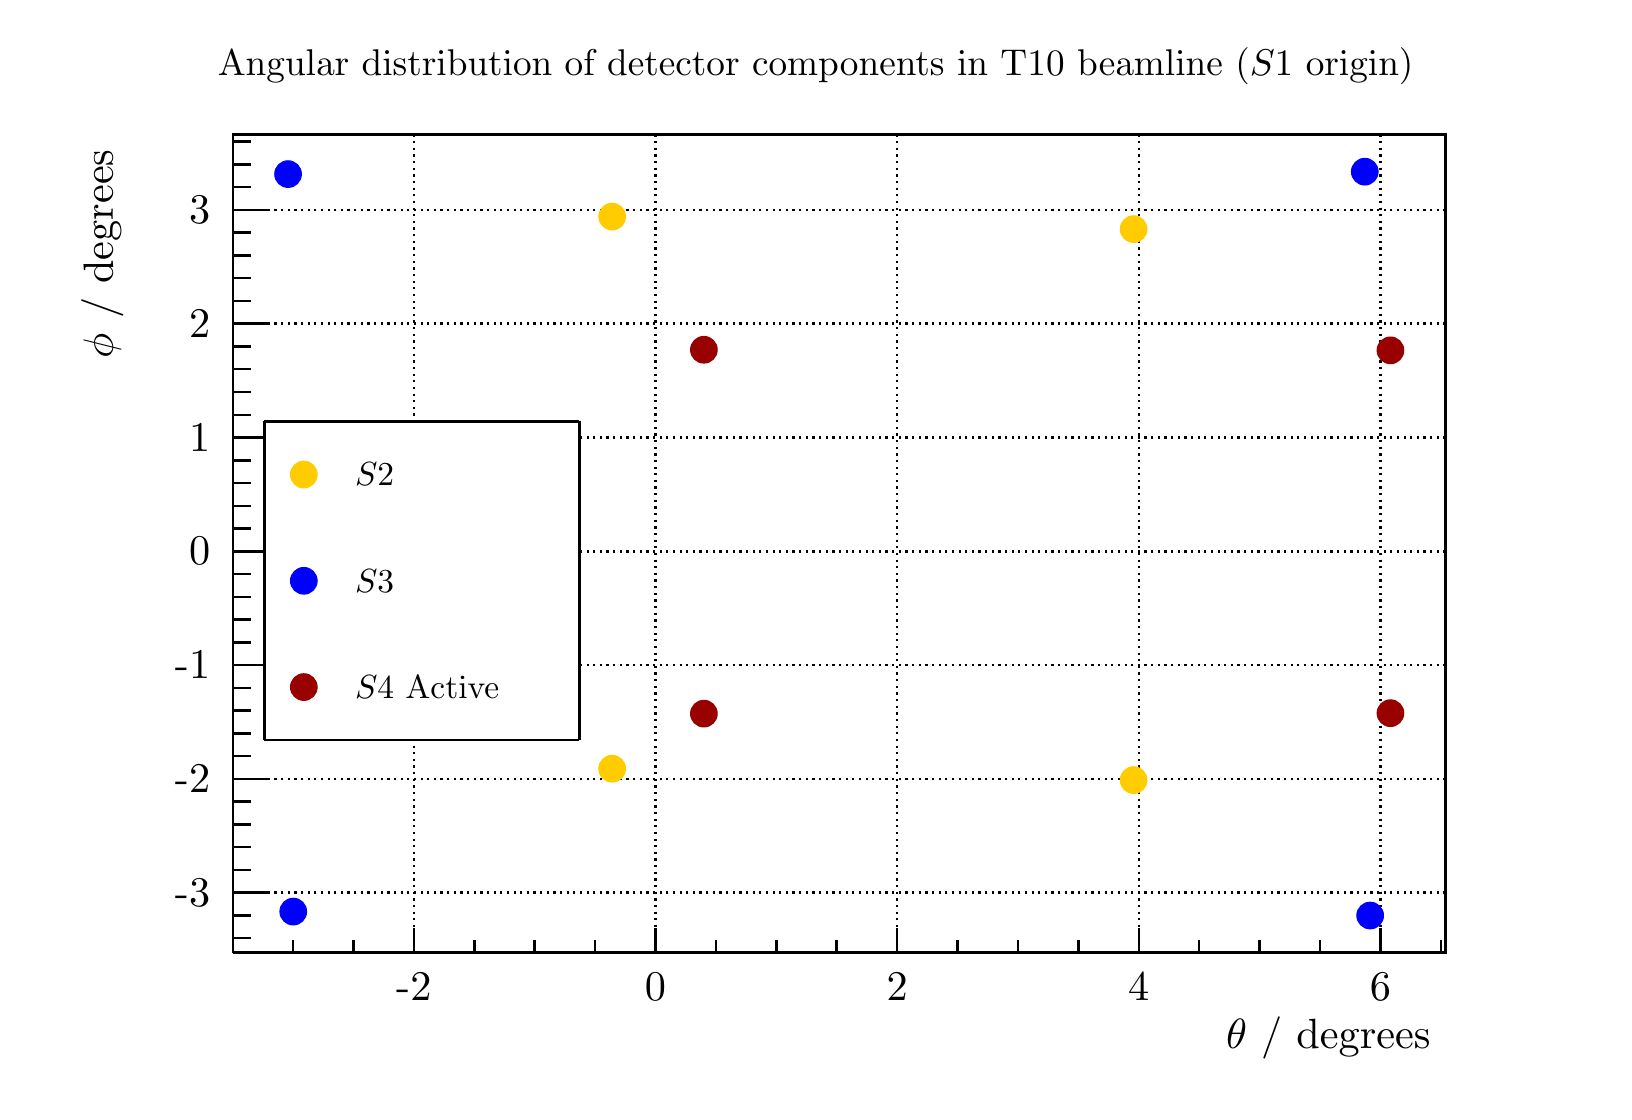
\begin{tikzpicture}
\pgfdeclareplotmark{cross} {
\pgfpathmoveto{\pgfpoint{-0.3\pgfplotmarksize}{\pgfplotmarksize}}
\pgfpathlineto{\pgfpoint{+0.3\pgfplotmarksize}{\pgfplotmarksize}}
\pgfpathlineto{\pgfpoint{+0.3\pgfplotmarksize}{0.3\pgfplotmarksize}}
\pgfpathlineto{\pgfpoint{+1\pgfplotmarksize}{0.3\pgfplotmarksize}}
\pgfpathlineto{\pgfpoint{+1\pgfplotmarksize}{-0.3\pgfplotmarksize}}
\pgfpathlineto{\pgfpoint{+0.3\pgfplotmarksize}{-0.3\pgfplotmarksize}}
\pgfpathlineto{\pgfpoint{+0.3\pgfplotmarksize}{-1.\pgfplotmarksize}}
\pgfpathlineto{\pgfpoint{-0.3\pgfplotmarksize}{-1.\pgfplotmarksize}}
\pgfpathlineto{\pgfpoint{-0.3\pgfplotmarksize}{-0.3\pgfplotmarksize}}
\pgfpathlineto{\pgfpoint{-1.\pgfplotmarksize}{-0.3\pgfplotmarksize}}
\pgfpathlineto{\pgfpoint{-1.\pgfplotmarksize}{0.3\pgfplotmarksize}}
\pgfpathlineto{\pgfpoint{-0.3\pgfplotmarksize}{0.3\pgfplotmarksize}}
\pgfpathclose
\pgfusepathqstroke
}
\pgfdeclareplotmark{cross*} {
\pgfpathmoveto{\pgfpoint{-0.3\pgfplotmarksize}{\pgfplotmarksize}}
\pgfpathlineto{\pgfpoint{+0.3\pgfplotmarksize}{\pgfplotmarksize}}
\pgfpathlineto{\pgfpoint{+0.3\pgfplotmarksize}{0.3\pgfplotmarksize}}
\pgfpathlineto{\pgfpoint{+1\pgfplotmarksize}{0.3\pgfplotmarksize}}
\pgfpathlineto{\pgfpoint{+1\pgfplotmarksize}{-0.3\pgfplotmarksize}}
\pgfpathlineto{\pgfpoint{+0.3\pgfplotmarksize}{-0.3\pgfplotmarksize}}
\pgfpathlineto{\pgfpoint{+0.3\pgfplotmarksize}{-1.\pgfplotmarksize}}
\pgfpathlineto{\pgfpoint{-0.3\pgfplotmarksize}{-1.\pgfplotmarksize}}
\pgfpathlineto{\pgfpoint{-0.3\pgfplotmarksize}{-0.3\pgfplotmarksize}}
\pgfpathlineto{\pgfpoint{-1.\pgfplotmarksize}{-0.3\pgfplotmarksize}}
\pgfpathlineto{\pgfpoint{-1.\pgfplotmarksize}{0.3\pgfplotmarksize}}
\pgfpathlineto{\pgfpoint{-0.3\pgfplotmarksize}{0.3\pgfplotmarksize}}
\pgfpathclose
\pgfusepathqfillstroke
}
\pgfdeclareplotmark{newstar} {
\pgfpathmoveto{\pgfqpoint{0pt}{\pgfplotmarksize}}
\pgfpathlineto{\pgfqpointpolar{44}{0.5\pgfplotmarksize}}
\pgfpathlineto{\pgfqpointpolar{18}{\pgfplotmarksize}}
\pgfpathlineto{\pgfqpointpolar{-20}{0.5\pgfplotmarksize}}
\pgfpathlineto{\pgfqpointpolar{-54}{\pgfplotmarksize}}
\pgfpathlineto{\pgfqpointpolar{-90}{0.5\pgfplotmarksize}}
\pgfpathlineto{\pgfqpointpolar{234}{\pgfplotmarksize}}
\pgfpathlineto{\pgfqpointpolar{198}{0.5\pgfplotmarksize}}
\pgfpathlineto{\pgfqpointpolar{162}{\pgfplotmarksize}}
\pgfpathlineto{\pgfqpointpolar{134}{0.5\pgfplotmarksize}}
\pgfpathclose
\pgfusepathqstroke
}
\pgfdeclareplotmark{newstar*} {
\pgfpathmoveto{\pgfqpoint{0pt}{\pgfplotmarksize}}
\pgfpathlineto{\pgfqpointpolar{44}{0.5\pgfplotmarksize}}
\pgfpathlineto{\pgfqpointpolar{18}{\pgfplotmarksize}}
\pgfpathlineto{\pgfqpointpolar{-20}{0.5\pgfplotmarksize}}
\pgfpathlineto{\pgfqpointpolar{-54}{\pgfplotmarksize}}
\pgfpathlineto{\pgfqpointpolar{-90}{0.5\pgfplotmarksize}}
\pgfpathlineto{\pgfqpointpolar{234}{\pgfplotmarksize}}
\pgfpathlineto{\pgfqpointpolar{198}{0.5\pgfplotmarksize}}
\pgfpathlineto{\pgfqpointpolar{162}{\pgfplotmarksize}}
\pgfpathlineto{\pgfqpointpolar{134}{0.5\pgfplotmarksize}}
\pgfpathclose
\pgfusepathqfillstroke
}
\definecolor{c}{rgb}{1,1,1};
\draw [color=c, fill=c] (0,0) rectangle (20,13.4957);
\draw [color=c, fill=c] (2.6,1.75444) rectangle (18,12.1461);
\definecolor{c}{rgb}{0,0,0};
\draw [c,line width=0.9] (2.6,1.75444) -- (2.6,12.1461) -- (18,12.1461) -- (18,1.75444) -- (2.6,1.75444);
\definecolor{c}{rgb}{1,1,1};
\draw [color=c, fill=c] (2.6,1.75444) rectangle (18,12.1461);
\definecolor{c}{rgb}{0,0,0};
\draw [c,line width=0.9] (2.6,1.75444) -- (2.6,12.1461) -- (18,12.1461) -- (18,1.75444) -- (2.6,1.75444);
\draw [c,line width=0.9] (2.6,1.75444) -- (18,1.75444);
\draw [c,dash pattern=on 0.80pt off 1.60pt ,line width=0.9] (4.89745,12.1461) -- (4.89745,1.75444);
\draw [c,dash pattern=on 0.80pt off 1.60pt ,line width=0.9] (7.96612,12.1461) -- (7.96612,1.75444);
\draw [c,dash pattern=on 0.80pt off 1.60pt ,line width=0.9] (11.0348,12.1461) -- (11.0348,1.75444);
\draw [c,dash pattern=on 0.80pt off 1.60pt ,line width=0.9] (14.1035,12.1461) -- (14.1035,1.75444);
\draw [c,dash pattern=on 0.80pt off 1.60pt ,line width=0.9] (17.1721,12.1461) -- (17.1721,1.75444);
\draw [c,dash pattern=on 0.80pt off 1.60pt ,line width=0.9] (4.89745,12.1461) -- (4.89745,1.75444);
\draw [c,dash pattern=on 0.80pt off 1.60pt ,line width=0.9] (17.1721,12.1461) -- (17.1721,1.75444);
\draw [c,line width=0.9] (2.6,1.75444) -- (2.6,12.1461);
\draw [c,dash pattern=on 0.80pt off 1.60pt ,line width=0.9] (18,2.51696) -- (2.6,2.51696);
\draw [c,dash pattern=on 0.80pt off 1.60pt ,line width=0.9] (18,3.96211) -- (2.6,3.96211);
\draw [c,dash pattern=on 0.80pt off 1.60pt ,line width=0.9] (18,5.40726) -- (2.6,5.40726);
\draw [c,dash pattern=on 0.80pt off 1.60pt ,line width=0.9] (18,6.85241) -- (2.6,6.85241);
\draw [c,dash pattern=on 0.80pt off 1.60pt ,line width=0.9] (18,8.29756) -- (2.6,8.29756);
\draw [c,dash pattern=on 0.80pt off 1.60pt ,line width=0.9] (18,9.74271) -- (2.6,9.74271);
\draw [c,dash pattern=on 0.80pt off 1.60pt ,line width=0.9] (18,11.1879) -- (2.6,11.1879);
\draw [c,dash pattern=on 0.80pt off 1.60pt ,line width=0.9] (18,2.51696) -- (2.6,2.51696);
\draw [c,dash pattern=on 0.80pt off 1.60pt ,line width=0.9] (18,11.1879) -- (2.6,11.1879);
\draw [c,line width=0.9] (2.6,1.75444) -- (18,1.75444);
\draw [c,line width=0.9] (4.89745,2.06619) -- (4.89745,1.75444);
\draw [c,line width=0.9] (5.66462,1.91032) -- (5.66462,1.75444);
\draw [c,line width=0.9] (6.43179,1.91032) -- (6.43179,1.75444);
\draw [c,line width=0.9] (7.19896,1.91032) -- (7.19896,1.75444);
\draw [c,line width=0.9] (7.96612,2.06619) -- (7.96612,1.75444);
\draw [c,line width=0.9] (8.73329,1.91032) -- (8.73329,1.75444);
\draw [c,line width=0.9] (9.50046,1.91032) -- (9.50046,1.75444);
\draw [c,line width=0.9] (10.2676,1.91032) -- (10.2676,1.75444);
\draw [c,line width=0.9] (11.0348,2.06619) -- (11.0348,1.75444);
\draw [c,line width=0.9] (11.802,1.91032) -- (11.802,1.75444);
\draw [c,line width=0.9] (12.5691,1.91032) -- (12.5691,1.75444);
\draw [c,line width=0.9] (13.3363,1.91032) -- (13.3363,1.75444);
\draw [c,line width=0.9] (14.1035,2.06619) -- (14.1035,1.75444);
\draw [c,line width=0.9] (14.8706,1.91032) -- (14.8706,1.75444);
\draw [c,line width=0.9] (15.6378,1.91032) -- (15.6378,1.75444);
\draw [c,line width=0.9] (16.405,1.91032) -- (16.405,1.75444);
\draw [c,line width=0.9] (17.1721,2.06619) -- (17.1721,1.75444);
\draw [c,line width=0.9] (4.89745,2.06619) -- (4.89745,1.75444);
\draw [c,line width=0.9] (4.13029,1.91032) -- (4.13029,1.75444);
\draw [c,line width=0.9] (3.36312,1.91032) -- (3.36312,1.75444);
\draw [c,line width=0.9] (17.1721,2.06619) -- (17.1721,1.75444);
\draw [c,line width=0.9] (17.9393,1.91032) -- (17.9393,1.75444);
\draw [anchor=base] (4.89745,1.14713) node[scale=1.52731, color=c, rotate=0]{-2};
\draw [anchor=base] (7.96612,1.14713) node[scale=1.52731, color=c, rotate=0]{0};
\draw [anchor=base] (11.0348,1.14713) node[scale=1.52731, color=c, rotate=0]{2};
\draw [anchor=base] (14.1035,1.14713) node[scale=1.52731, color=c, rotate=0]{4};
\draw [anchor=base] (17.1721,1.14713) node[scale=1.52731, color=c, rotate=0]{6};
\draw [anchor= east] (18,0.674785) node[scale=1.52731, color=c, rotate=0]{$\theta$ / degrees};
\draw [c,line width=0.9] (2.6,1.75444) -- (2.6,12.1461);
\draw [c,line width=0.9] (3.062,2.51696) -- (2.6,2.51696);
\draw [c,line width=0.9] (2.831,2.80599) -- (2.6,2.80599);
\draw [c,line width=0.9] (2.831,3.09502) -- (2.6,3.09502);
\draw [c,line width=0.9] (2.831,3.38405) -- (2.6,3.38405);
\draw [c,line width=0.9] (2.831,3.67308) -- (2.6,3.67308);
\draw [c,line width=0.9] (3.062,3.96211) -- (2.6,3.96211);
\draw [c,line width=0.9] (2.831,4.25114) -- (2.6,4.25114);
\draw [c,line width=0.9] (2.831,4.54017) -- (2.6,4.54017);
\draw [c,line width=0.9] (2.831,4.8292) -- (2.6,4.8292);
\draw [c,line width=0.9] (2.831,5.11823) -- (2.6,5.11823);
\draw [c,line width=0.9] (3.062,5.40726) -- (2.6,5.40726);
\draw [c,line width=0.9] (2.831,5.69629) -- (2.6,5.69629);
\draw [c,line width=0.9] (2.831,5.98532) -- (2.6,5.98532);
\draw [c,line width=0.9] (2.831,6.27435) -- (2.6,6.27435);
\draw [c,line width=0.9] (2.831,6.56338) -- (2.6,6.56338);
\draw [c,line width=0.9] (3.062,6.85241) -- (2.6,6.85241);
\draw [c,line width=0.9] (2.831,7.14144) -- (2.6,7.14144);
\draw [c,line width=0.9] (2.831,7.43047) -- (2.6,7.43047);
\draw [c,line width=0.9] (2.831,7.7195) -- (2.6,7.7195);
\draw [c,line width=0.9] (2.831,8.00853) -- (2.6,8.00853);
\draw [c,line width=0.9] (3.062,8.29756) -- (2.6,8.29756);
\draw [c,line width=0.9] (2.831,8.58659) -- (2.6,8.58659);
\draw [c,line width=0.9] (2.831,8.87562) -- (2.6,8.87562);
\draw [c,line width=0.9] (2.831,9.16465) -- (2.6,9.16465);
\draw [c,line width=0.9] (2.831,9.45368) -- (2.6,9.45368);
\draw [c,line width=0.9] (3.062,9.74271) -- (2.6,9.74271);
\draw [c,line width=0.9] (2.831,10.0317) -- (2.6,10.0317);
\draw [c,line width=0.9] (2.831,10.3208) -- (2.6,10.3208);
\draw [c,line width=0.9] (2.831,10.6098) -- (2.6,10.6098);
\draw [c,line width=0.9] (2.831,10.8988) -- (2.6,10.8988);
\draw [c,line width=0.9] (3.062,11.1879) -- (2.6,11.1879);
\draw [c,line width=0.9] (3.062,2.51696) -- (2.6,2.51696);
\draw [c,line width=0.9] (2.831,2.22793) -- (2.6,2.22793);
\draw [c,line width=0.9] (2.831,1.9389) -- (2.6,1.9389);
\draw [c,line width=0.9] (3.062,11.1879) -- (2.6,11.1879);
\draw [c,line width=0.9] (2.831,11.4769) -- (2.6,11.4769);
\draw [c,line width=0.9] (2.831,11.7659) -- (2.6,11.7659);
\draw [c,line width=0.9] (2.831,12.055) -- (2.6,12.055);
\draw [anchor= east] (2.5,2.51696) node[scale=1.52731, color=c, rotate=0]{-3};
\draw [anchor= east] (2.5,3.96211) node[scale=1.52731, color=c, rotate=0]{-2};
\draw [anchor= east] (2.5,5.40726) node[scale=1.52731, color=c, rotate=0]{-1};
\draw [anchor= east] (2.5,6.85241) node[scale=1.52731, color=c, rotate=0]{0};
\draw [anchor= east] (2.5,8.29756) node[scale=1.52731, color=c, rotate=0]{1};
\draw [anchor= east] (2.5,9.74271) node[scale=1.52731, color=c, rotate=0]{2};
\draw [anchor= east] (2.5,11.1879) node[scale=1.52731, color=c, rotate=0]{3};
\draw [anchor= east] (0.940974,12.1461) node[scale=1.52731, color=c, rotate=90]{$\phi$ / degrees};
\definecolor{c}{rgb}{1,0.8,0};
\foreach \P in {(7.41566,11.1035), (7.41566,4.09158), (14.0382,3.94708), (14.0382,10.9445)}{\draw[mark options={color=c,fill=c},mark size=4.804805pt,mark=*] plot coordinates {\P};}
\definecolor{c}{rgb}{0,0,1};
\foreach \P in {(3.3,11.6431), (16.9742,11.6738), (3.36572,2.27713), (17.0424,2.22679)}{\draw[mark options={color=c,fill=c},mark size=4.804805pt,mark=*] plot coordinates {\P};}
\definecolor{c}{rgb}{0.6,0,0};
\foreach \P in {(8.58078,9.41224), (17.3,9.4046), (8.58078,4.79087), (17.3,4.79702)}{\draw[mark options={color=c,fill=c},mark size=4.804805pt,mark=*] plot coordinates {\P};}
\definecolor{c}{rgb}{1,1,1};
\draw [color=c, fill=c] (3,4.45358) rectangle (7,8.50229);
\definecolor{c}{rgb}{0,0,0};
\draw [c,line width=0.9] (3,4.45358) -- (7,4.45358);
\draw [c,line width=0.9] (7,4.45358) -- (7,8.50229);
\draw [c,line width=0.9] (7,8.50229) -- (3,8.50229);
\draw [c,line width=0.9] (3,8.50229) -- (3,4.45358);
\draw [anchor= west] (4,7.82751) node[scale=1.20912, color=c, rotate=0]{$S2$};
\definecolor{c}{rgb}{1,0.8,0};
\foreach \P in {(3.5,7.82751)}{\draw[mark options={color=c,fill=c},mark size=4.804805pt,mark=*] plot coordinates {\P};}
\definecolor{c}{rgb}{0,0,0};
\draw [anchor= west] (4,6.47794) node[scale=1.20912, color=c, rotate=0]{$S3$};
\definecolor{c}{rgb}{0,0,1};
\foreach \P in {(3.5,6.47794)}{\draw[mark options={color=c,fill=c},mark size=4.804805pt,mark=*] plot coordinates {\P};}
\definecolor{c}{rgb}{0,0,0};
\draw [anchor= west] (4,5.12837) node[scale=1.20912, color=c, rotate=0]{$S4$ Active};
\definecolor{c}{rgb}{0.6,0,0};
\foreach \P in {(3.5,5.12837)}{\draw[mark options={color=c,fill=c},mark size=4.804805pt,mark=*] plot coordinates {\P};}
\definecolor{c}{rgb}{0,0,0};
\draw (10,13.0156) node[scale=1.34549, color=c, rotate=0]{Angular distribution of detector components in T10 beamline ($S1$ origin)};
\end{tikzpicture}

    \end{adjustbox}
    \centering
    \caption{Diagram showing the angular location of the extremities of the timing points. The coordinate system used has the origin at the $\mathit{S1}$ timing point, with the $x$ axis running parallel to the nominal beam axis.}
    \label{fig:beamAng}
  \end{minipage}
  \hfill
  \begin{minipage}{0.49\textwidth}
    \begin{adjustbox}{max totalsize={\textwidth}{0.5\textheight}, center}
      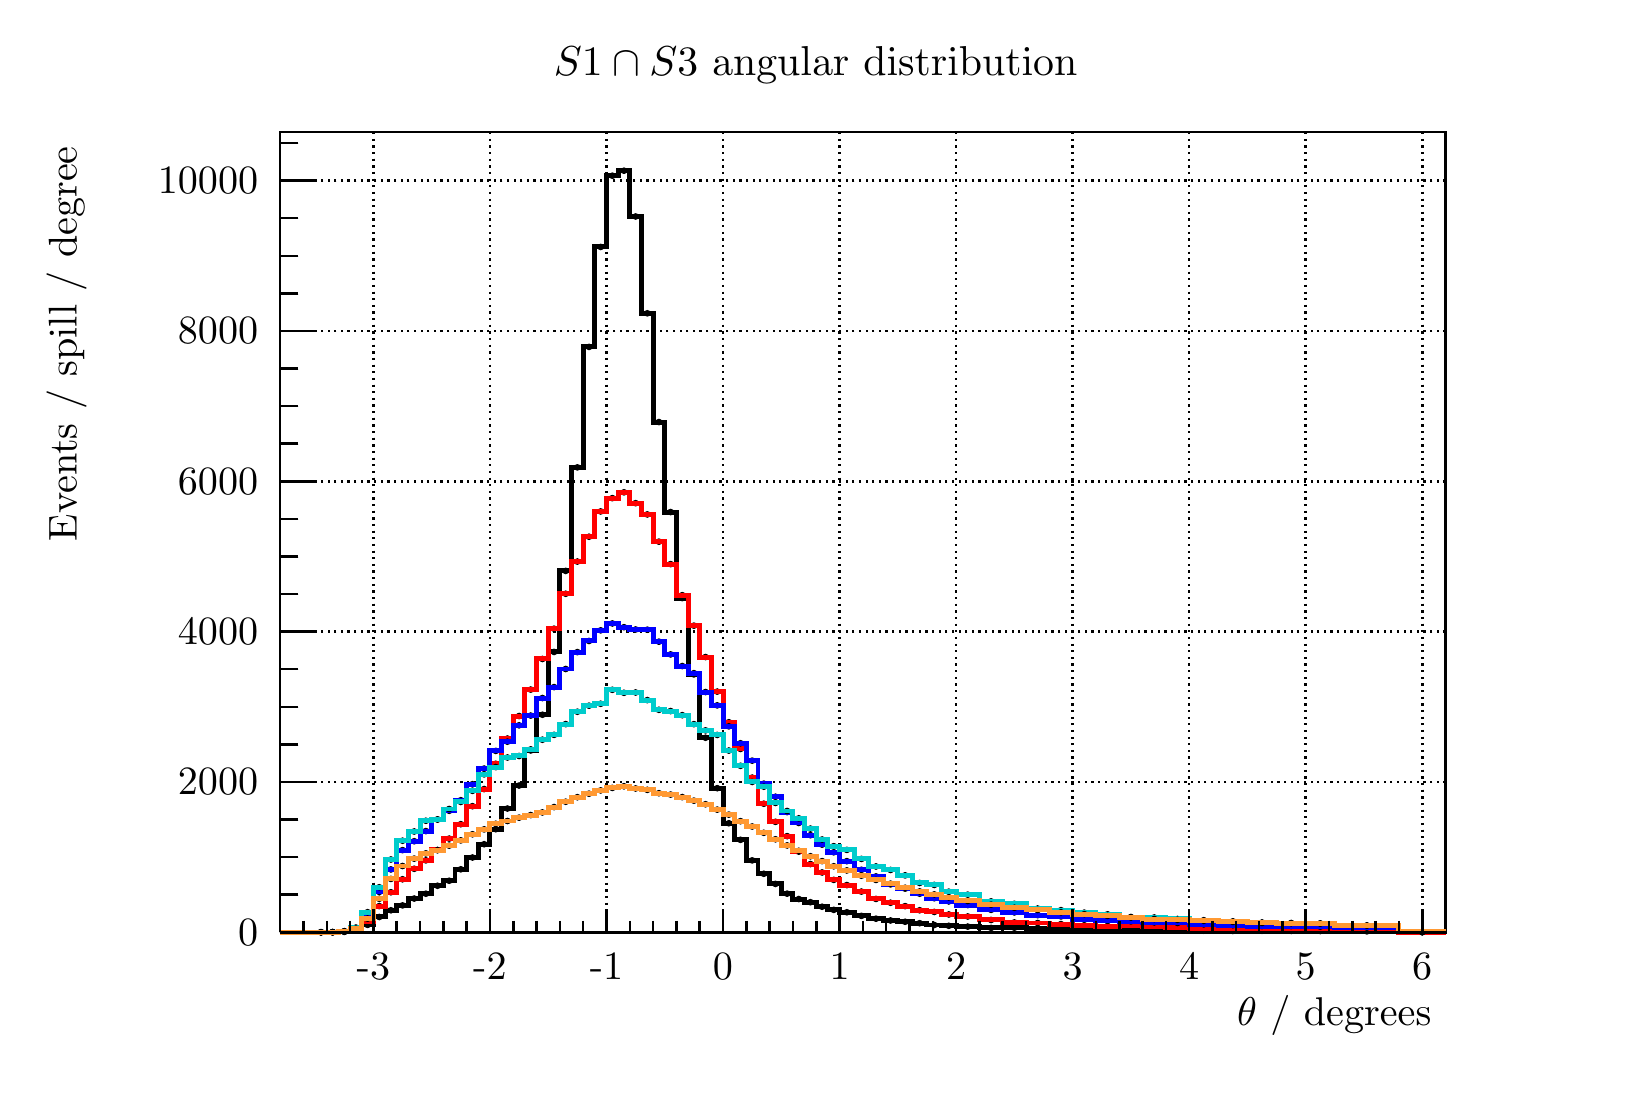
\begin{tikzpicture}
\pgfdeclareplotmark{cross} {
\pgfpathmoveto{\pgfpoint{-0.3\pgfplotmarksize}{\pgfplotmarksize}}
\pgfpathlineto{\pgfpoint{+0.3\pgfplotmarksize}{\pgfplotmarksize}}
\pgfpathlineto{\pgfpoint{+0.3\pgfplotmarksize}{0.3\pgfplotmarksize}}
\pgfpathlineto{\pgfpoint{+1\pgfplotmarksize}{0.3\pgfplotmarksize}}
\pgfpathlineto{\pgfpoint{+1\pgfplotmarksize}{-0.3\pgfplotmarksize}}
\pgfpathlineto{\pgfpoint{+0.3\pgfplotmarksize}{-0.3\pgfplotmarksize}}
\pgfpathlineto{\pgfpoint{+0.3\pgfplotmarksize}{-1.\pgfplotmarksize}}
\pgfpathlineto{\pgfpoint{-0.3\pgfplotmarksize}{-1.\pgfplotmarksize}}
\pgfpathlineto{\pgfpoint{-0.3\pgfplotmarksize}{-0.3\pgfplotmarksize}}
\pgfpathlineto{\pgfpoint{-1.\pgfplotmarksize}{-0.3\pgfplotmarksize}}
\pgfpathlineto{\pgfpoint{-1.\pgfplotmarksize}{0.3\pgfplotmarksize}}
\pgfpathlineto{\pgfpoint{-0.3\pgfplotmarksize}{0.3\pgfplotmarksize}}
\pgfpathclose
\pgfusepathqstroke
}
\pgfdeclareplotmark{cross*} {
\pgfpathmoveto{\pgfpoint{-0.3\pgfplotmarksize}{\pgfplotmarksize}}
\pgfpathlineto{\pgfpoint{+0.3\pgfplotmarksize}{\pgfplotmarksize}}
\pgfpathlineto{\pgfpoint{+0.3\pgfplotmarksize}{0.3\pgfplotmarksize}}
\pgfpathlineto{\pgfpoint{+1\pgfplotmarksize}{0.3\pgfplotmarksize}}
\pgfpathlineto{\pgfpoint{+1\pgfplotmarksize}{-0.3\pgfplotmarksize}}
\pgfpathlineto{\pgfpoint{+0.3\pgfplotmarksize}{-0.3\pgfplotmarksize}}
\pgfpathlineto{\pgfpoint{+0.3\pgfplotmarksize}{-1.\pgfplotmarksize}}
\pgfpathlineto{\pgfpoint{-0.3\pgfplotmarksize}{-1.\pgfplotmarksize}}
\pgfpathlineto{\pgfpoint{-0.3\pgfplotmarksize}{-0.3\pgfplotmarksize}}
\pgfpathlineto{\pgfpoint{-1.\pgfplotmarksize}{-0.3\pgfplotmarksize}}
\pgfpathlineto{\pgfpoint{-1.\pgfplotmarksize}{0.3\pgfplotmarksize}}
\pgfpathlineto{\pgfpoint{-0.3\pgfplotmarksize}{0.3\pgfplotmarksize}}
\pgfpathclose
\pgfusepathqfillstroke
}
\pgfdeclareplotmark{newstar} {
\pgfpathmoveto{\pgfqpoint{0pt}{\pgfplotmarksize}}
\pgfpathlineto{\pgfqpointpolar{44}{0.5\pgfplotmarksize}}
\pgfpathlineto{\pgfqpointpolar{18}{\pgfplotmarksize}}
\pgfpathlineto{\pgfqpointpolar{-20}{0.5\pgfplotmarksize}}
\pgfpathlineto{\pgfqpointpolar{-54}{\pgfplotmarksize}}
\pgfpathlineto{\pgfqpointpolar{-90}{0.5\pgfplotmarksize}}
\pgfpathlineto{\pgfqpointpolar{234}{\pgfplotmarksize}}
\pgfpathlineto{\pgfqpointpolar{198}{0.5\pgfplotmarksize}}
\pgfpathlineto{\pgfqpointpolar{162}{\pgfplotmarksize}}
\pgfpathlineto{\pgfqpointpolar{134}{0.5\pgfplotmarksize}}
\pgfpathclose
\pgfusepathqstroke
}
\pgfdeclareplotmark{newstar*} {
\pgfpathmoveto{\pgfqpoint{0pt}{\pgfplotmarksize}}
\pgfpathlineto{\pgfqpointpolar{44}{0.5\pgfplotmarksize}}
\pgfpathlineto{\pgfqpointpolar{18}{\pgfplotmarksize}}
\pgfpathlineto{\pgfqpointpolar{-20}{0.5\pgfplotmarksize}}
\pgfpathlineto{\pgfqpointpolar{-54}{\pgfplotmarksize}}
\pgfpathlineto{\pgfqpointpolar{-90}{0.5\pgfplotmarksize}}
\pgfpathlineto{\pgfqpointpolar{234}{\pgfplotmarksize}}
\pgfpathlineto{\pgfqpointpolar{198}{0.5\pgfplotmarksize}}
\pgfpathlineto{\pgfqpointpolar{162}{\pgfplotmarksize}}
\pgfpathlineto{\pgfqpointpolar{134}{0.5\pgfplotmarksize}}
\pgfpathclose
\pgfusepathqfillstroke
}
\definecolor{c}{rgb}{1,1,1};
\draw [color=c, fill=c] (0,0) rectangle (20,13.1973);
\draw [color=c, fill=c] (3.2,1.71565) rectangle (18,11.8776);
\definecolor{c}{rgb}{0,0,0};
\draw [c,line width=0.9] (3.2,1.71565) -- (3.2,11.8776) -- (18,11.8776) -- (18,1.71565) -- (3.2,1.71565);
\definecolor{c}{rgb}{1,1,1};
\draw [color=c, fill=c] (3.2,1.71565) rectangle (18,11.8776);
\definecolor{c}{rgb}{0,0,0};
\draw [c,line width=0.9] (3.2,1.71565) -- (3.2,11.8776) -- (18,11.8776) -- (18,1.71565) -- (3.2,1.71565);
\draw [c,line width=0.9] (3.2,1.71565) -- (18,1.71565);
\draw [c,dash pattern=on 0.80pt off 1.60pt ,line width=0.9] (4.384,11.8776) -- (4.384,1.71565);
\draw [c,dash pattern=on 0.80pt off 1.60pt ,line width=0.9] (5.864,11.8776) -- (5.864,1.71565);
\draw [c,dash pattern=on 0.80pt off 1.60pt ,line width=0.9] (7.344,11.8776) -- (7.344,1.71565);
\draw [c,dash pattern=on 0.80pt off 1.60pt ,line width=0.9] (8.824,11.8776) -- (8.824,1.71565);
\draw [c,dash pattern=on 0.80pt off 1.60pt ,line width=0.9] (10.304,11.8776) -- (10.304,1.71565);
\draw [c,dash pattern=on 0.80pt off 1.60pt ,line width=0.9] (11.784,11.8776) -- (11.784,1.71565);
\draw [c,dash pattern=on 0.80pt off 1.60pt ,line width=0.9] (13.264,11.8776) -- (13.264,1.71565);
\draw [c,dash pattern=on 0.80pt off 1.60pt ,line width=0.9] (14.744,11.8776) -- (14.744,1.71565);
\draw [c,dash pattern=on 0.80pt off 1.60pt ,line width=0.9] (16.224,11.8776) -- (16.224,1.71565);
\draw [c,dash pattern=on 0.80pt off 1.60pt ,line width=0.9] (17.704,11.8776) -- (17.704,1.71565);
\draw [c,dash pattern=on 0.80pt off 1.60pt ,line width=0.9] (4.384,11.8776) -- (4.384,1.71565);
\draw [c,dash pattern=on 0.80pt off 1.60pt ,line width=0.9] (17.704,11.8776) -- (17.704,1.71565);
\draw [c,line width=0.9] (3.2,1.71565) -- (3.2,11.8776);
\draw [c,dash pattern=on 0.80pt off 1.60pt ,line width=0.9] (18,1.71565) -- (3.2,1.71565);
\draw [c,dash pattern=on 0.80pt off 1.60pt ,line width=0.9] (18,3.62476) -- (3.2,3.62476);
\draw [c,dash pattern=on 0.80pt off 1.60pt ,line width=0.9] (18,5.53388) -- (3.2,5.53388);
\draw [c,dash pattern=on 0.80pt off 1.60pt ,line width=0.9] (18,7.443) -- (3.2,7.443);
\draw [c,dash pattern=on 0.80pt off 1.60pt ,line width=0.9] (18,9.35212) -- (3.2,9.35212);
\draw [c,dash pattern=on 0.80pt off 1.60pt ,line width=0.9] (18,11.2612) -- (3.2,11.2612);
\draw [c,dash pattern=on 0.80pt off 1.60pt ,line width=0.9] (18,11.2612) -- (3.2,11.2612);
\definecolor{c}{rgb}{0,0,0.6};
\draw [c,line width=0.9] (3.2,1.71565) -- (3.348,1.71565) -- (3.348,1.71565) -- (3.496,1.71565) -- (3.496,1.71565) -- (3.644,1.71565) -- (3.644,1.71565) -- (3.792,1.71565) -- (3.792,1.71565) -- (3.94,1.71565) -- (3.94,1.71565) -- (4.088,1.71565) --
 (4.088,1.71565) -- (4.236,1.71565) -- (4.236,1.71565) -- (4.384,1.71565) -- (4.384,1.71565) -- (4.532,1.71565) -- (4.532,1.71565) -- (4.68,1.71565) -- (4.68,1.71565) -- (4.828,1.71565) -- (4.828,1.71565) -- (4.976,1.71565) -- (4.976,1.71565) --
 (5.124,1.71565) -- (5.124,1.71565) -- (5.272,1.71565) -- (5.272,1.71565) -- (5.42,1.71565) -- (5.42,1.71565) -- (5.568,1.71565) -- (5.568,1.71565) -- (5.716,1.71565) -- (5.716,1.71565) -- (5.864,1.71565) -- (5.864,1.71565) -- (6.012,1.71565) --
 (6.012,1.71565) -- (6.16,1.71565) -- (6.16,1.71565) -- (6.308,1.71565) -- (6.308,1.71565) -- (6.456,1.71565) -- (6.456,1.71565) -- (6.604,1.71565) -- (6.604,1.71565) -- (6.752,1.71565) -- (6.752,1.71565) -- (6.9,1.71565) -- (6.9,1.71565) --
 (7.048,1.71565) -- (7.048,1.71565) -- (7.196,1.71565) -- (7.196,1.71565) -- (7.344,1.71565) -- (7.344,1.71565) -- (7.492,1.71565) -- (7.492,1.71565) -- (7.64,1.71565) -- (7.64,1.71565) -- (7.788,1.71565) -- (7.788,1.71565) -- (7.936,1.71565) --
 (7.936,1.71565) -- (8.084,1.71565) -- (8.084,1.71565) -- (8.232,1.71565) -- (8.232,1.71565) -- (8.38,1.71565) -- (8.38,1.71565) -- (8.528,1.71565) -- (8.528,1.71565) -- (8.676,1.71565) -- (8.676,1.71565) -- (8.824,1.71565) -- (8.824,1.71565) --
 (8.972,1.71565) -- (8.972,1.71565) -- (9.12,1.71565) -- (9.12,1.71565) -- (9.268,1.71565) -- (9.268,1.71565) -- (9.416,1.71565) -- (9.416,1.71565) -- (9.564,1.71565) -- (9.564,1.71565) -- (9.712,1.71565) -- (9.712,1.71565) -- (9.86,1.71565) --
 (9.86,1.71565) -- (10.008,1.71565) -- (10.008,1.71565) -- (10.156,1.71565) -- (10.156,1.71565) -- (10.304,1.71565) -- (10.304,1.71565) -- (10.489,1.71565) -- (10.489,1.71565) -- (10.674,1.71565) -- (10.674,1.71565) -- (10.859,1.71565) --
 (10.859,1.71565) -- (11.044,1.71565) -- (11.044,1.71565) -- (11.229,1.71565) -- (11.229,1.71565) -- (11.414,1.71565) -- (11.414,1.71565) -- (11.599,1.71565) -- (11.599,1.71565) -- (11.784,1.71565) -- (11.784,1.71565) -- (12.08,1.71565) --
 (12.08,1.71565) -- (12.376,1.71565) -- (12.376,1.71565) -- (12.672,1.71565) -- (12.672,1.71565) -- (12.968,1.71565) -- (12.968,1.71565) -- (13.264,1.71565) -- (13.264,1.71565) -- (13.56,1.71565) -- (13.56,1.71565) -- (13.856,1.71565) --
 (13.856,1.71565) -- (14.152,1.71565) -- (14.152,1.71565) -- (14.448,1.71565) -- (14.448,1.71565) -- (14.744,1.71565) -- (14.744,1.71565) -- (15.114,1.71565) -- (15.114,1.71565) -- (15.484,1.71565) -- (15.484,1.71565) -- (15.854,1.71565) --
 (15.854,1.71565) -- (16.224,1.71565) -- (16.224,1.71565) -- (16.594,1.71565) -- (16.594,1.71565) -- (17.408,1.71565) -- (17.408,1.71565) -- (18,1.71565);
\definecolor{c}{rgb}{0,0,0};
\draw [c,line width=0.9] (3.2,1.71565) -- (18,1.71565);
\draw [c,line width=0.9] (4.384,2.00863) -- (4.384,1.71565);
\draw [c,line width=0.9] (4.68,1.86214) -- (4.68,1.71565);
\draw [c,line width=0.9] (4.976,1.86214) -- (4.976,1.71565);
\draw [c,line width=0.9] (5.272,1.86214) -- (5.272,1.71565);
\draw [c,line width=0.9] (5.568,1.86214) -- (5.568,1.71565);
\draw [c,line width=0.9] (5.864,2.00863) -- (5.864,1.71565);
\draw [c,line width=0.9] (6.16,1.86214) -- (6.16,1.71565);
\draw [c,line width=0.9] (6.456,1.86214) -- (6.456,1.71565);
\draw [c,line width=0.9] (6.752,1.86214) -- (6.752,1.71565);
\draw [c,line width=0.9] (7.048,1.86214) -- (7.048,1.71565);
\draw [c,line width=0.9] (7.344,2.00863) -- (7.344,1.71565);
\draw [c,line width=0.9] (7.64,1.86214) -- (7.64,1.71565);
\draw [c,line width=0.9] (7.936,1.86214) -- (7.936,1.71565);
\draw [c,line width=0.9] (8.232,1.86214) -- (8.232,1.71565);
\draw [c,line width=0.9] (8.528,1.86214) -- (8.528,1.71565);
\draw [c,line width=0.9] (8.824,2.00863) -- (8.824,1.71565);
\draw [c,line width=0.9] (9.12,1.86214) -- (9.12,1.71565);
\draw [c,line width=0.9] (9.416,1.86214) -- (9.416,1.71565);
\draw [c,line width=0.9] (9.712,1.86214) -- (9.712,1.71565);
\draw [c,line width=0.9] (10.008,1.86214) -- (10.008,1.71565);
\draw [c,line width=0.9] (10.304,2.00863) -- (10.304,1.71565);
\draw [c,line width=0.9] (10.6,1.86214) -- (10.6,1.71565);
\draw [c,line width=0.9] (10.896,1.86214) -- (10.896,1.71565);
\draw [c,line width=0.9] (11.192,1.86214) -- (11.192,1.71565);
\draw [c,line width=0.9] (11.488,1.86214) -- (11.488,1.71565);
\draw [c,line width=0.9] (11.784,2.00863) -- (11.784,1.71565);
\draw [c,line width=0.9] (12.08,1.86214) -- (12.08,1.71565);
\draw [c,line width=0.9] (12.376,1.86214) -- (12.376,1.71565);
\draw [c,line width=0.9] (12.672,1.86214) -- (12.672,1.71565);
\draw [c,line width=0.9] (12.968,1.86214) -- (12.968,1.71565);
\draw [c,line width=0.9] (13.264,2.00863) -- (13.264,1.71565);
\draw [c,line width=0.9] (13.56,1.86214) -- (13.56,1.71565);
\draw [c,line width=0.9] (13.856,1.86214) -- (13.856,1.71565);
\draw [c,line width=0.9] (14.152,1.86214) -- (14.152,1.71565);
\draw [c,line width=0.9] (14.448,1.86214) -- (14.448,1.71565);
\draw [c,line width=0.9] (14.744,2.00863) -- (14.744,1.71565);
\draw [c,line width=0.9] (15.04,1.86214) -- (15.04,1.71565);
\draw [c,line width=0.9] (15.336,1.86214) -- (15.336,1.71565);
\draw [c,line width=0.9] (15.632,1.86214) -- (15.632,1.71565);
\draw [c,line width=0.9] (15.928,1.86214) -- (15.928,1.71565);
\draw [c,line width=0.9] (16.224,2.00863) -- (16.224,1.71565);
\draw [c,line width=0.9] (16.52,1.86214) -- (16.52,1.71565);
\draw [c,line width=0.9] (16.816,1.86214) -- (16.816,1.71565);
\draw [c,line width=0.9] (17.112,1.86214) -- (17.112,1.71565);
\draw [c,line width=0.9] (17.408,1.86214) -- (17.408,1.71565);
\draw [c,line width=0.9] (17.704,2.00863) -- (17.704,1.71565);
\draw [c,line width=0.9] (4.384,2.00863) -- (4.384,1.71565);
\draw [c,line width=0.9] (4.088,1.86214) -- (4.088,1.71565);
\draw [c,line width=0.9] (3.792,1.86214) -- (3.792,1.71565);
\draw [c,line width=0.9] (3.496,1.86214) -- (3.496,1.71565);
\draw [c,line width=0.9] (17.704,2.00863) -- (17.704,1.71565);
\draw [anchor=base] (4.384,1.12177) node[scale=1.45043, color=c, rotate=0]{-3};
\draw [anchor=base] (5.864,1.12177) node[scale=1.45043, color=c, rotate=0]{-2};
\draw [anchor=base] (7.344,1.12177) node[scale=1.45043, color=c, rotate=0]{-1};
\draw [anchor=base] (8.824,1.12177) node[scale=1.45043, color=c, rotate=0]{0};
\draw [anchor=base] (10.304,1.12177) node[scale=1.45043, color=c, rotate=0]{1};
\draw [anchor=base] (11.784,1.12177) node[scale=1.45043, color=c, rotate=0]{2};
\draw [anchor=base] (13.264,1.12177) node[scale=1.45043, color=c, rotate=0]{3};
\draw [anchor=base] (14.744,1.12177) node[scale=1.45043, color=c, rotate=0]{4};
\draw [anchor=base] (16.224,1.12177) node[scale=1.45043, color=c, rotate=0]{5};
\draw [anchor=base] (17.704,1.12177) node[scale=1.45043, color=c, rotate=0]{6};
\draw [anchor= east] (18,0.659864) node[scale=1.45043, color=c, rotate=0]{$\theta$ / degrees};
\draw [c,line width=0.9] (3.2,1.71565) -- (3.2,11.8776);
\draw [c,line width=0.9] (3.662,1.71565) -- (3.2,1.71565);
\draw [c,line width=0.9] (3.431,2.19293) -- (3.2,2.19293);
\draw [c,line width=0.9] (3.431,2.67021) -- (3.2,2.67021);
\draw [c,line width=0.9] (3.431,3.14748) -- (3.2,3.14748);
\draw [c,line width=0.9] (3.662,3.62476) -- (3.2,3.62476);
\draw [c,line width=0.9] (3.431,4.10204) -- (3.2,4.10204);
\draw [c,line width=0.9] (3.431,4.57932) -- (3.2,4.57932);
\draw [c,line width=0.9] (3.431,5.0566) -- (3.2,5.0566);
\draw [c,line width=0.9] (3.662,5.53388) -- (3.2,5.53388);
\draw [c,line width=0.9] (3.431,6.01116) -- (3.2,6.01116);
\draw [c,line width=0.9] (3.431,6.48844) -- (3.2,6.48844);
\draw [c,line width=0.9] (3.431,6.96572) -- (3.2,6.96572);
\draw [c,line width=0.9] (3.662,7.443) -- (3.2,7.443);
\draw [c,line width=0.9] (3.431,7.92028) -- (3.2,7.92028);
\draw [c,line width=0.9] (3.431,8.39756) -- (3.2,8.39756);
\draw [c,line width=0.9] (3.431,8.87484) -- (3.2,8.87484);
\draw [c,line width=0.9] (3.662,9.35212) -- (3.2,9.35212);
\draw [c,line width=0.9] (3.431,9.8294) -- (3.2,9.8294);
\draw [c,line width=0.9] (3.431,10.3067) -- (3.2,10.3067);
\draw [c,line width=0.9] (3.431,10.784) -- (3.2,10.784);
\draw [c,line width=0.9] (3.662,11.2612) -- (3.2,11.2612);
\draw [c,line width=0.9] (3.662,11.2612) -- (3.2,11.2612);
\draw [c,line width=0.9] (3.431,11.7385) -- (3.2,11.7385);
\draw [anchor= east] (3.1,1.71565) node[scale=1.45043, color=c, rotate=0]{0};
\draw [anchor= east] (3.1,3.62476) node[scale=1.45043, color=c, rotate=0]{2000};
\draw [anchor= east] (3.1,5.53388) node[scale=1.45043, color=c, rotate=0]{4000};
\draw [anchor= east] (3.1,7.443) node[scale=1.45043, color=c, rotate=0]{6000};
\draw [anchor= east] (3.1,9.35212) node[scale=1.45043, color=c, rotate=0]{8000};
\draw [anchor= east] (3.1,11.2612) node[scale=1.45043, color=c, rotate=0]{10000};
\draw [anchor= east] (0.485714,11.8776) node[scale=1.45043, color=c, rotate=90]{ Events / spill / degree};
\draw [c,line width=1.8] (3.866,1.71595) -- (3.866,1.71598);
\draw [c,line width=1.8] (3.866,1.71598) -- (3.866,1.71602);
\foreach \P in {(3.866,1.71598)}{\draw[mark options={color=c,fill=c},mark size=2.402402pt,mark=*,mark size=1pt] plot coordinates {\P};}
\draw [c,line width=1.8] (4.014,1.72602) -- (4.014,1.72622);
\draw [c,line width=1.8] (4.014,1.72622) -- (4.014,1.72642);
\foreach \P in {(4.014,1.72622)}{\draw[mark options={color=c,fill=c},mark size=2.402402pt,mark=*,mark size=1pt] plot coordinates {\P};}
\draw [c,line width=1.8] (4.162,1.74717) -- (4.162,1.74753);
\draw [c,line width=1.8] (4.162,1.74753) -- (4.162,1.74788);
\foreach \P in {(4.162,1.74753)}{\draw[mark options={color=c,fill=c},mark size=2.402402pt,mark=*,mark size=1pt] plot coordinates {\P};}
\draw [c,line width=1.8] (4.31,1.80928) -- (4.31,1.80989);
\draw [c,line width=1.8] (4.31,1.80989) -- (4.31,1.81049);
\foreach \P in {(4.31,1.80989)}{\draw[mark options={color=c,fill=c},mark size=2.402402pt,mark=*,mark size=1pt] plot coordinates {\P};}
\draw [c,line width=1.8] (4.458,1.90916) -- (4.458,1.91003);
\draw [c,line width=1.8] (4.458,1.91003) -- (4.458,1.91089);
\foreach \P in {(4.458,1.91003)}{\draw[mark options={color=c,fill=c},mark size=2.402402pt,mark=*,mark size=1pt] plot coordinates {\P};}
\draw [c,line width=1.8] (4.606,1.99401) -- (4.606,1.99505);
\draw [c,line width=1.8] (4.606,1.99505) -- (4.606,1.99608);
\foreach \P in {(4.606,1.99505)}{\draw[mark options={color=c,fill=c},mark size=2.402402pt,mark=*,mark size=1pt] plot coordinates {\P};}
\draw [c,line width=1.8] (4.754,2.05623) -- (4.754,2.05738);
\draw [c,line width=1.8] (4.754,2.05738) -- (4.754,2.05852);
\foreach \P in {(4.754,2.05738)}{\draw[mark options={color=c,fill=c},mark size=2.402402pt,mark=*,mark size=1pt] plot coordinates {\P};}
\draw [c,line width=1.8] (4.902,2.14291) -- (4.902,2.1442);
\draw [c,line width=1.8] (4.902,2.1442) -- (4.902,2.14548);
\foreach \P in {(4.902,2.1442)}{\draw[mark options={color=c,fill=c},mark size=2.402402pt,mark=*,mark size=1pt] plot coordinates {\P};}
\draw [c,line width=1.8] (5.05,2.20396) -- (5.05,2.20534);
\draw [c,line width=1.8] (5.05,2.20534) -- (5.05,2.20671);
\foreach \P in {(5.05,2.20534)}{\draw[mark options={color=c,fill=c},mark size=2.402402pt,mark=*,mark size=1pt] plot coordinates {\P};}
\draw [c,line width=1.8] (5.198,2.30504) -- (5.198,2.30655);
\draw [c,line width=1.8] (5.198,2.30655) -- (5.198,2.30806);
\foreach \P in {(5.198,2.30655)}{\draw[mark options={color=c,fill=c},mark size=2.402402pt,mark=*,mark size=1pt] plot coordinates {\P};}
\draw [c,line width=1.8] (5.346,2.36846) -- (5.346,2.37004);
\draw [c,line width=1.8] (5.346,2.37004) -- (5.346,2.37162);
\foreach \P in {(5.346,2.37004)}{\draw[mark options={color=c,fill=c},mark size=2.402402pt,mark=*,mark size=1pt] plot coordinates {\P};}
\draw [c,line width=1.8] (5.494,2.51391) -- (5.494,2.51566);
\draw [c,line width=1.8] (5.494,2.51566) -- (5.494,2.51742);
\foreach \P in {(5.494,2.51566)}{\draw[mark options={color=c,fill=c},mark size=2.402402pt,mark=*,mark size=1pt] plot coordinates {\P};}
\draw [c,line width=1.8] (5.642,2.66342) -- (5.642,2.66533);
\draw [c,line width=1.8] (5.642,2.66533) -- (5.642,2.66724);
\foreach \P in {(5.642,2.66533)}{\draw[mark options={color=c,fill=c},mark size=2.402402pt,mark=*,mark size=1pt] plot coordinates {\P};}
\draw [c,line width=1.8] (5.79,2.83225) -- (5.79,2.83433);
\draw [c,line width=1.8] (5.79,2.83433) -- (5.79,2.83641);
\foreach \P in {(5.79,2.83433)}{\draw[mark options={color=c,fill=c},mark size=2.402402pt,mark=*,mark size=1pt] plot coordinates {\P};}
\draw [c,line width=1.8] (5.938,3.0229) -- (5.938,3.02514);
\draw [c,line width=1.8] (5.938,3.02514) -- (5.938,3.02739);
\foreach \P in {(5.938,3.02514)}{\draw[mark options={color=c,fill=c},mark size=2.402402pt,mark=*,mark size=1pt] plot coordinates {\P};}
\draw [c,line width=1.8] (6.086,3.28485) -- (6.086,3.28731);
\draw [c,line width=1.8] (6.086,3.28731) -- (6.086,3.28977);
\foreach \P in {(6.086,3.28731)}{\draw[mark options={color=c,fill=c},mark size=2.402402pt,mark=*,mark size=1pt] plot coordinates {\P};}
\draw [c,line width=1.8] (6.234,3.57673) -- (6.234,3.57941);
\draw [c,line width=1.8] (6.234,3.57941) -- (6.234,3.58209);
\foreach \P in {(6.234,3.57941)}{\draw[mark options={color=c,fill=c},mark size=2.402402pt,mark=*,mark size=1pt] plot coordinates {\P};}
\draw [c,line width=1.8] (6.382,4.02164) -- (6.382,4.02462);
\draw [c,line width=1.8] (6.382,4.02462) -- (6.382,4.0276);
\foreach \P in {(6.382,4.02462)}{\draw[mark options={color=c,fill=c},mark size=2.402402pt,mark=*,mark size=1pt] plot coordinates {\P};}
\draw [c,line width=1.8] (6.53,4.47508) -- (6.53,4.47834);
\draw [c,line width=1.8] (6.53,4.47834) -- (6.53,4.4816);
\foreach \P in {(6.53,4.47834)}{\draw[mark options={color=c,fill=c},mark size=2.402402pt,mark=*,mark size=1pt] plot coordinates {\P};}
\draw [c,line width=1.8] (6.678,5.2722) -- (6.678,5.27591);
\draw [c,line width=1.8] (6.678,5.27591) -- (6.678,5.27961);
\foreach \P in {(6.678,5.27591)}{\draw[mark options={color=c,fill=c},mark size=2.402402pt,mark=*,mark size=1pt] plot coordinates {\P};}
\draw [c,line width=1.8] (6.826,6.30096) -- (6.826,6.30517);
\draw [c,line width=1.8] (6.826,6.30517) -- (6.826,6.30937);
\foreach \P in {(6.826,6.30517)}{\draw[mark options={color=c,fill=c},mark size=2.402402pt,mark=*,mark size=1pt] plot coordinates {\P};}
\draw [c,line width=1.8] (6.974,7.61533) -- (6.974,7.6201);
\draw [c,line width=1.8] (6.974,7.6201) -- (6.974,7.62487);
\foreach \P in {(6.974,7.6201)}{\draw[mark options={color=c,fill=c},mark size=2.402402pt,mark=*,mark size=1pt] plot coordinates {\P};}
\draw [c,line width=1.8] (7.122,9.1446) -- (7.122,9.14996);
\draw [c,line width=1.8] (7.122,9.14996) -- (7.122,9.15531);
\foreach \P in {(7.122,9.14996)}{\draw[mark options={color=c,fill=c},mark size=2.402402pt,mark=*,mark size=1pt] plot coordinates {\P};}
\draw [c,line width=1.8] (7.27,10.4135) -- (7.27,10.4193);
\draw [c,line width=1.8] (7.27,10.4193) -- (7.27,10.4251);
\foreach \P in {(7.27,10.4193)}{\draw[mark options={color=c,fill=c},mark size=2.402402pt,mark=*,mark size=1pt] plot coordinates {\P};}
\draw [c,line width=1.8] (7.418,11.3178) -- (7.418,11.3239);
\draw [c,line width=1.8] (7.418,11.3239) -- (7.418,11.33);
\foreach \P in {(7.418,11.3239)}{\draw[mark options={color=c,fill=c},mark size=2.402402pt,mark=*,mark size=1pt] plot coordinates {\P};}
\draw [c,line width=1.8] (7.566,11.3814) -- (7.566,11.3875);
\draw [c,line width=1.8] (7.566,11.3875) -- (7.566,11.3937);
\foreach \P in {(7.566,11.3875)}{\draw[mark options={color=c,fill=c},mark size=2.402402pt,mark=*,mark size=1pt] plot coordinates {\P};}
\draw [c,line width=1.8] (7.714,10.8002) -- (7.714,10.8062);
\draw [c,line width=1.8] (7.714,10.8062) -- (7.714,10.8121);
\foreach \P in {(7.714,10.8062)}{\draw[mark options={color=c,fill=c},mark size=2.402402pt,mark=*,mark size=1pt] plot coordinates {\P};}
\draw [c,line width=1.8] (7.862,9.57131) -- (7.862,9.57681);
\draw [c,line width=1.8] (7.862,9.57681) -- (7.862,9.58232);
\foreach \P in {(7.862,9.57681)}{\draw[mark options={color=c,fill=c},mark size=2.402402pt,mark=*,mark size=1pt] plot coordinates {\P};}
\draw [c,line width=1.8] (8.01,8.19073) -- (8.01,8.19572);
\draw [c,line width=1.8] (8.01,8.19572) -- (8.01,8.20072);
\foreach \P in {(8.01,8.19572)}{\draw[mark options={color=c,fill=c},mark size=2.402402pt,mark=*,mark size=1pt] plot coordinates {\P};}
\draw [c,line width=1.8] (8.158,7.04789) -- (8.158,7.05242);
\draw [c,line width=1.8] (8.158,7.05242) -- (8.158,7.05696);
\foreach \P in {(8.158,7.05242)}{\draw[mark options={color=c,fill=c},mark size=2.402402pt,mark=*,mark size=1pt] plot coordinates {\P};}
\draw [c,line width=1.8] (8.306,5.95642) -- (8.306,5.96046);
\draw [c,line width=1.8] (8.306,5.96046) -- (8.306,5.9645);
\foreach \P in {(8.306,5.96046)}{\draw[mark options={color=c,fill=c},mark size=2.402402pt,mark=*,mark size=1pt] plot coordinates {\P};}
\draw [c,line width=1.8] (8.454,4.98731) -- (8.454,4.99086);
\draw [c,line width=1.8] (8.454,4.99086) -- (8.454,4.99441);
\foreach \P in {(8.454,4.99086)}{\draw[mark options={color=c,fill=c},mark size=2.402402pt,mark=*,mark size=1pt] plot coordinates {\P};}
\draw [c,line width=1.8] (8.602,4.18348) -- (8.602,4.18655);
\draw [c,line width=1.8] (8.602,4.18655) -- (8.602,4.18964);
\foreach \P in {(8.602,4.18655)}{\draw[mark options={color=c,fill=c},mark size=2.402402pt,mark=*,mark size=1pt] plot coordinates {\P};}
\draw [c,line width=1.8] (8.75,3.54324) -- (8.75,3.5459);
\draw [c,line width=1.8] (8.75,3.5459) -- (8.75,3.54855);
\foreach \P in {(8.75,3.5459)}{\draw[mark options={color=c,fill=c},mark size=2.402402pt,mark=*,mark size=1pt] plot coordinates {\P};}
\draw [c,line width=1.8] (8.898,3.09817) -- (8.898,3.10048);
\draw [c,line width=1.8] (8.898,3.10048) -- (8.898,3.10279);
\foreach \P in {(8.898,3.10048)}{\draw[mark options={color=c,fill=c},mark size=2.402402pt,mark=*,mark size=1pt] plot coordinates {\P};}
\draw [c,line width=1.8] (9.046,2.88775) -- (9.046,2.88987);
\draw [c,line width=1.8] (9.046,2.88987) -- (9.046,2.892);
\foreach \P in {(9.046,2.88987)}{\draw[mark options={color=c,fill=c},mark size=2.402402pt,mark=*,mark size=1pt] plot coordinates {\P};}
\draw [c,line width=1.8] (9.194,2.62707) -- (9.194,2.62894);
\draw [c,line width=1.8] (9.194,2.62894) -- (9.194,2.63082);
\foreach \P in {(9.194,2.62894)}{\draw[mark options={color=c,fill=c},mark size=2.402402pt,mark=*,mark size=1pt] plot coordinates {\P};}
\draw [c,line width=1.8] (9.342,2.45685) -- (9.342,2.45855);
\draw [c,line width=1.8] (9.342,2.45855) -- (9.342,2.46025);
\foreach \P in {(9.342,2.45855)}{\draw[mark options={color=c,fill=c},mark size=2.402402pt,mark=*,mark size=1pt] plot coordinates {\P};}
\draw [c,line width=1.8] (9.49,2.32864) -- (9.49,2.33018);
\draw [c,line width=1.8] (9.49,2.33018) -- (9.49,2.33172);
\foreach \P in {(9.49,2.33018)}{\draw[mark options={color=c,fill=c},mark size=2.402402pt,mark=*,mark size=1pt] plot coordinates {\P};}
\draw [c,line width=1.8] (9.638,2.20478) -- (9.638,2.20616);
\draw [c,line width=1.8] (9.638,2.20616) -- (9.638,2.20753);
\foreach \P in {(9.638,2.20616)}{\draw[mark options={color=c,fill=c},mark size=2.402402pt,mark=*,mark size=1pt] plot coordinates {\P};}
\draw [c,line width=1.8] (9.786,2.13673) -- (9.786,2.138);
\draw [c,line width=1.8] (9.786,2.138) -- (9.786,2.13928);
\foreach \P in {(9.786,2.138)}{\draw[mark options={color=c,fill=c},mark size=2.402402pt,mark=*,mark size=1pt] plot coordinates {\P};}
\draw [c,line width=1.8] (9.934,2.09656) -- (9.934,2.09777);
\draw [c,line width=1.8] (9.934,2.09777) -- (9.934,2.09898);
\foreach \P in {(9.934,2.09777)}{\draw[mark options={color=c,fill=c},mark size=2.402402pt,mark=*,mark size=1pt] plot coordinates {\P};}
\draw [c,line width=1.8] (10.082,2.03883) -- (10.082,2.03995);
\draw [c,line width=1.8] (10.082,2.03995) -- (10.082,2.04107);
\foreach \P in {(10.082,2.03995)}{\draw[mark options={color=c,fill=c},mark size=2.402402pt,mark=*,mark size=1pt] plot coordinates {\P};}
\draw [c,line width=1.8] (10.23,1.99928) -- (10.23,2.00033);
\draw [c,line width=1.8] (10.23,2.00033) -- (10.23,2.00138);
\foreach \P in {(10.23,2.00033)}{\draw[mark options={color=c,fill=c},mark size=2.402402pt,mark=*,mark size=1pt] plot coordinates {\P};}
\draw [c,line width=1.8] (10.3965,1.96875) -- (10.3965,1.96986);
\draw [c,line width=1.8] (10.3965,1.96986) -- (10.3965,1.97098);
\foreach \P in {(10.3965,1.96986)}{\draw[mark options={color=c,fill=c},mark size=2.402402pt,mark=*,mark size=1pt] plot coordinates {\P};}
\draw [c,line width=1.8] (10.5815,1.92309) -- (10.5815,1.92409);
\draw [c,line width=1.8] (10.5815,1.92409) -- (10.5815,1.92509);
\foreach \P in {(10.5815,1.92409)}{\draw[mark options={color=c,fill=c},mark size=2.402402pt,mark=*,mark size=1pt] plot coordinates {\P};}
\draw [c,line width=1.8] (10.7665,1.88738) -- (10.7665,1.88829);
\draw [c,line width=1.8] (10.7665,1.88829) -- (10.7665,1.88921);
\foreach \P in {(10.7665,1.88829)}{\draw[mark options={color=c,fill=c},mark size=2.402402pt,mark=*,mark size=1pt] plot coordinates {\P};}
\draw [c,line width=1.8] (10.9515,1.86492) -- (10.9515,1.86577);
\draw [c,line width=1.8] (10.9515,1.86577) -- (10.9515,1.86662);
\foreach \P in {(10.9515,1.86577)}{\draw[mark options={color=c,fill=c},mark size=2.402402pt,mark=*,mark size=1pt] plot coordinates {\P};}
\draw [c,line width=1.8] (11.1365,1.84845) -- (11.1365,1.84925);
\draw [c,line width=1.8] (11.1365,1.84925) -- (11.1365,1.85006);
\foreach \P in {(11.1365,1.84925)}{\draw[mark options={color=c,fill=c},mark size=2.402402pt,mark=*,mark size=1pt] plot coordinates {\P};}
\draw [c,line width=1.8] (11.3215,1.8305) -- (11.3215,1.83124);
\draw [c,line width=1.8] (11.3215,1.83124) -- (11.3215,1.83199);
\foreach \P in {(11.3215,1.83124)}{\draw[mark options={color=c,fill=c},mark size=2.402402pt,mark=*,mark size=1pt] plot coordinates {\P};}
\draw [c,line width=1.8] (11.5065,1.80763) -- (11.5065,1.8083);
\draw [c,line width=1.8] (11.5065,1.8083) -- (11.5065,1.80897);
\foreach \P in {(11.5065,1.8083)}{\draw[mark options={color=c,fill=c},mark size=2.402402pt,mark=*,mark size=1pt] plot coordinates {\P};}
\draw [c,line width=1.8] (11.6915,1.79744) -- (11.6915,1.79807);
\draw [c,line width=1.8] (11.6915,1.79807) -- (11.6915,1.7987);
\foreach \P in {(11.6915,1.79807)}{\draw[mark options={color=c,fill=c},mark size=2.402402pt,mark=*,mark size=1pt] plot coordinates {\P};}
\draw [c,line width=1.8] (11.932,1.78715) -- (11.932,1.7879);
\draw [c,line width=1.8] (11.932,1.7879) -- (11.932,1.78865);
\foreach \P in {(11.932,1.7879)}{\draw[mark options={color=c,fill=c},mark size=2.402402pt,mark=*,mark size=1pt] plot coordinates {\P};}
\draw [c,line width=1.8] (12.228,1.77104) -- (12.228,1.77169);
\draw [c,line width=1.8] (12.228,1.77169) -- (12.228,1.77235);
\foreach \P in {(12.228,1.77169)}{\draw[mark options={color=c,fill=c},mark size=2.402402pt,mark=*,mark size=1pt] plot coordinates {\P};}
\draw [c,line width=1.8] (12.524,1.77292) -- (12.524,1.77359);
\draw [c,line width=1.8] (12.524,1.77359) -- (12.524,1.77426);
\foreach \P in {(12.524,1.77359)}{\draw[mark options={color=c,fill=c},mark size=2.402402pt,mark=*,mark size=1pt] plot coordinates {\P};}
\draw [c,line width=1.8] (12.82,1.76345) -- (12.82,1.76406);
\draw [c,line width=1.8] (12.82,1.76406) -- (12.82,1.76467);
\foreach \P in {(12.82,1.76406)}{\draw[mark options={color=c,fill=c},mark size=2.402402pt,mark=*,mark size=1pt] plot coordinates {\P};}
\draw [c,line width=1.8] (13.116,1.75696) -- (13.116,1.75753);
\draw [c,line width=1.8] (13.116,1.75753) -- (13.116,1.7581);
\foreach \P in {(13.116,1.75753)}{\draw[mark options={color=c,fill=c},mark size=2.402402pt,mark=*,mark size=1pt] plot coordinates {\P};}
\draw [c,line width=1.8] (13.412,1.75321) -- (13.412,1.75375);
\draw [c,line width=1.8] (13.412,1.75375) -- (13.412,1.75429);
\foreach \P in {(13.412,1.75375)}{\draw[mark options={color=c,fill=c},mark size=2.402402pt,mark=*,mark size=1pt] plot coordinates {\P};}
\draw [c,line width=1.8] (13.708,1.74621) -- (13.708,1.7467);
\draw [c,line width=1.8] (13.708,1.7467) -- (13.708,1.74719);
\foreach \P in {(13.708,1.7467)}{\draw[mark options={color=c,fill=c},mark size=2.402402pt,mark=*,mark size=1pt] plot coordinates {\P};}
\draw [c,line width=1.8] (14.004,1.7477) -- (14.004,1.74821);
\draw [c,line width=1.8] (14.004,1.74821) -- (14.004,1.74872);
\foreach \P in {(14.004,1.74821)}{\draw[mark options={color=c,fill=c},mark size=2.402402pt,mark=*,mark size=1pt] plot coordinates {\P};}
\draw [c,line width=1.8] (14.3,1.73968) -- (14.3,1.74012);
\draw [c,line width=1.8] (14.3,1.74012) -- (14.3,1.74055);
\foreach \P in {(14.3,1.74012)}{\draw[mark options={color=c,fill=c},mark size=2.402402pt,mark=*,mark size=1pt] plot coordinates {\P};}
\draw [c,line width=1.8] (14.596,1.74118) -- (14.596,1.74162);
\draw [c,line width=1.8] (14.596,1.74162) -- (14.596,1.74207);
\foreach \P in {(14.596,1.74162)}{\draw[mark options={color=c,fill=c},mark size=2.402402pt,mark=*,mark size=1pt] plot coordinates {\P};}
\draw [c,line width=1.8] (14.929,1.73604) -- (14.929,1.73649);
\draw [c,line width=1.8] (14.929,1.73649) -- (14.929,1.73694);
\foreach \P in {(14.929,1.73649)}{\draw[mark options={color=c,fill=c},mark size=2.402402pt,mark=*,mark size=1pt] plot coordinates {\P};}
\draw [c,line width=1.8] (15.299,1.73286) -- (15.299,1.73327);
\draw [c,line width=1.8] (15.299,1.73327) -- (15.299,1.73368);
\foreach \P in {(15.299,1.73327)}{\draw[mark options={color=c,fill=c},mark size=2.402402pt,mark=*,mark size=1pt] plot coordinates {\P};}
\draw [c,line width=1.8] (15.669,1.73382) -- (15.669,1.73425);
\draw [c,line width=1.8] (15.669,1.73425) -- (15.669,1.73467);
\foreach \P in {(15.669,1.73425)}{\draw[mark options={color=c,fill=c},mark size=2.402402pt,mark=*,mark size=1pt] plot coordinates {\P};}
\draw [c,line width=1.8] (16.039,1.73304) -- (16.039,1.73345);
\draw [c,line width=1.8] (16.039,1.73345) -- (16.039,1.73387);
\foreach \P in {(16.039,1.73345)}{\draw[mark options={color=c,fill=c},mark size=2.402402pt,mark=*,mark size=1pt] plot coordinates {\P};}
\draw [c,line width=1.8] (16.409,1.73173) -- (16.409,1.73212);
\draw [c,line width=1.8] (16.409,1.73212) -- (16.409,1.73252);
\foreach \P in {(16.409,1.73212)}{\draw[mark options={color=c,fill=c},mark size=2.402402pt,mark=*,mark size=1pt] plot coordinates {\P};}
\draw [c,line width=1.8] (17.001,1.72718) -- (17.001,1.72768);
\draw [c,line width=1.8] (17.001,1.72768) -- (17.001,1.72818);
\foreach \P in {(17.001,1.72768)}{\draw[mark options={color=c,fill=c},mark size=2.402402pt,mark=*,mark size=1pt] plot coordinates {\P};}
\draw [c,line width=1.8] (17.704,1.71687) -- (17.704,1.71711);
\draw [c,line width=1.8] (17.704,1.71711) -- (17.704,1.71734);
\foreach \P in {(17.704,1.71711)}{\draw[mark options={color=c,fill=c},mark size=2.402402pt,mark=*,mark size=1pt] plot coordinates {\P};}
\draw [c,line width=1.8] (3.2,1.71565) -- (3.348,1.71565) -- (3.348,1.71565) -- (3.496,1.71565) -- (3.496,1.71565) -- (3.644,1.71565) -- (3.644,1.71565) -- (3.792,1.71565) -- (3.792,1.71565) -- (3.94,1.71565) -- (3.94,1.72622) -- (4.088,1.72622) --
 (4.088,1.74753) -- (4.236,1.74753) -- (4.236,1.80989) -- (4.384,1.80989) -- (4.384,1.91003) -- (4.532,1.91003) -- (4.532,1.99505) -- (4.68,1.99505) -- (4.68,2.05738) -- (4.828,2.05738) -- (4.828,2.1442) -- (4.976,2.1442) -- (4.976,2.20534) --
 (5.124,2.20534) -- (5.124,2.30655) -- (5.272,2.30655) -- (5.272,2.37004) -- (5.42,2.37004) -- (5.42,2.51566) -- (5.568,2.51566) -- (5.568,2.66533) -- (5.716,2.66533) -- (5.716,2.83433) -- (5.864,2.83433) -- (5.864,3.02514) -- (6.012,3.02514) --
 (6.012,3.28731) -- (6.16,3.28731) -- (6.16,3.57941) -- (6.308,3.57941) -- (6.308,4.02462) -- (6.456,4.02462) -- (6.456,4.47834) -- (6.604,4.47834) -- (6.604,5.27591) -- (6.752,5.27591) -- (6.752,6.30517) -- (6.9,6.30517) -- (6.9,7.6201) --
 (7.048,7.6201) -- (7.048,9.14996) -- (7.196,9.14996) -- (7.196,10.4193) -- (7.344,10.4193) -- (7.344,11.3239) -- (7.492,11.3239) -- (7.492,11.3875) -- (7.64,11.3875) -- (7.64,10.8062) -- (7.788,10.8062) -- (7.788,9.57681) -- (7.936,9.57681) --
 (7.936,8.19572) -- (8.084,8.19572) -- (8.084,7.05242) -- (8.232,7.05242) -- (8.232,5.96046) -- (8.38,5.96046) -- (8.38,4.99086) -- (8.528,4.99086) -- (8.528,4.18655) -- (8.676,4.18655) -- (8.676,3.5459) -- (8.824,3.5459) -- (8.824,3.10048) --
 (8.972,3.10048) -- (8.972,2.88987) -- (9.12,2.88987) -- (9.12,2.62894) -- (9.268,2.62894) -- (9.268,2.45855) -- (9.416,2.45855) -- (9.416,2.33018) -- (9.564,2.33018) -- (9.564,2.20616) -- (9.712,2.20616) -- (9.712,2.138) -- (9.86,2.138) --
 (9.86,2.09777) -- (10.008,2.09777) -- (10.008,2.03995) -- (10.156,2.03995) -- (10.156,2.00033) -- (10.304,2.00033) -- (10.304,1.96986) -- (10.489,1.96986) -- (10.489,1.92409) -- (10.674,1.92409) -- (10.674,1.88829) -- (10.859,1.88829) --
 (10.859,1.86577) -- (11.044,1.86577) -- (11.044,1.84925) -- (11.229,1.84925) -- (11.229,1.83124) -- (11.414,1.83124) -- (11.414,1.8083) -- (11.599,1.8083) -- (11.599,1.79807) -- (11.784,1.79807) -- (11.784,1.7879) -- (12.08,1.7879) --
 (12.08,1.77169) -- (12.376,1.77169) -- (12.376,1.77359) -- (12.672,1.77359) -- (12.672,1.76406) -- (12.968,1.76406) -- (12.968,1.75753) -- (13.264,1.75753) -- (13.264,1.75375) -- (13.56,1.75375) -- (13.56,1.7467) -- (13.856,1.7467) --
 (13.856,1.74821) -- (14.152,1.74821) -- (14.152,1.74012) -- (14.448,1.74012) -- (14.448,1.74162) -- (14.744,1.74162) -- (14.744,1.73649) -- (15.114,1.73649) -- (15.114,1.73327) -- (15.484,1.73327) -- (15.484,1.73425) -- (15.854,1.73425) --
 (15.854,1.73345) -- (16.224,1.73345) -- (16.224,1.73212) -- (16.594,1.73212) -- (16.594,1.72768) -- (17.408,1.72768) -- (17.408,1.71711) -- (18,1.71711);
\definecolor{c}{rgb}{1,0,0};
\draw [c,line width=1.8] (3.718,1.71585) -- (3.718,1.71587);
\draw [c,line width=1.8] (3.718,1.71587) -- (3.718,1.71589);
\definecolor{c}{rgb}{0,0,0};
\foreach \P in {(3.718,1.71587)}{\draw[mark options={color=c,fill=c},mark size=2.402402pt,mark=*,mark size=1pt] plot coordinates {\P};}
\definecolor{c}{rgb}{1,0,0};
\draw [c,line width=1.8] (3.866,1.71663) -- (3.866,1.71668);
\draw [c,line width=1.8] (3.866,1.71668) -- (3.866,1.71673);
\definecolor{c}{rgb}{0,0,0};
\foreach \P in {(3.866,1.71668)}{\draw[mark options={color=c,fill=c},mark size=2.402402pt,mark=*,mark size=1pt] plot coordinates {\P};}
\definecolor{c}{rgb}{1,0,0};
\draw [c,line width=1.8] (4.014,1.72073) -- (4.014,1.72084);
\draw [c,line width=1.8] (4.014,1.72084) -- (4.014,1.72096);
\definecolor{c}{rgb}{0,0,0};
\foreach \P in {(4.014,1.72084)}{\draw[mark options={color=c,fill=c},mark size=2.402402pt,mark=*,mark size=1pt] plot coordinates {\P};}
\definecolor{c}{rgb}{1,0,0};
\draw [c,line width=1.8] (4.162,1.74902) -- (4.162,1.74931);
\draw [c,line width=1.8] (4.162,1.74931) -- (4.162,1.74961);
\definecolor{c}{rgb}{0,0,0};
\foreach \P in {(4.162,1.74931)}{\draw[mark options={color=c,fill=c},mark size=2.402402pt,mark=*,mark size=1pt] plot coordinates {\P};}
\definecolor{c}{rgb}{1,0,0};
\draw [c,line width=1.8] (4.31,1.85326) -- (4.31,1.85387);
\draw [c,line width=1.8] (4.31,1.85387) -- (4.31,1.85447);
\definecolor{c}{rgb}{0,0,0};
\foreach \P in {(4.31,1.85387)}{\draw[mark options={color=c,fill=c},mark size=2.402402pt,mark=*,mark size=1pt] plot coordinates {\P};}
\definecolor{c}{rgb}{1,0,0};
\draw [c,line width=1.8] (4.458,2.04758) -- (4.458,2.04852);
\draw [c,line width=1.8] (4.458,2.04852) -- (4.458,2.04946);
\definecolor{c}{rgb}{0,0,0};
\foreach \P in {(4.458,2.04852)}{\draw[mark options={color=c,fill=c},mark size=2.402402pt,mark=*,mark size=1pt] plot coordinates {\P};}
\definecolor{c}{rgb}{1,0,0};
\draw [c,line width=1.8] (4.606,2.22314) -- (4.606,2.2243);
\draw [c,line width=1.8] (4.606,2.2243) -- (4.606,2.22545);
\definecolor{c}{rgb}{0,0,0};
\foreach \P in {(4.606,2.2243)}{\draw[mark options={color=c,fill=c},mark size=2.402402pt,mark=*,mark size=1pt] plot coordinates {\P};}
\definecolor{c}{rgb}{1,0,0};
\draw [c,line width=1.8] (4.754,2.38765) -- (4.754,2.38899);
\draw [c,line width=1.8] (4.754,2.38899) -- (4.754,2.39032);
\definecolor{c}{rgb}{0,0,0};
\foreach \P in {(4.754,2.38899)}{\draw[mark options={color=c,fill=c},mark size=2.402402pt,mark=*,mark size=1pt] plot coordinates {\P};}
\definecolor{c}{rgb}{1,0,0};
\draw [c,line width=1.8] (4.902,2.52091) -- (4.902,2.52237);
\draw [c,line width=1.8] (4.902,2.52237) -- (4.902,2.52383);
\definecolor{c}{rgb}{0,0,0};
\foreach \P in {(4.902,2.52237)}{\draw[mark options={color=c,fill=c},mark size=2.402402pt,mark=*,mark size=1pt] plot coordinates {\P};}
\definecolor{c}{rgb}{1,0,0};
\draw [c,line width=1.8] (5.05,2.62813) -- (5.05,2.62968);
\draw [c,line width=1.8] (5.05,2.62968) -- (5.05,2.63123);
\definecolor{c}{rgb}{0,0,0};
\foreach \P in {(5.05,2.62968)}{\draw[mark options={color=c,fill=c},mark size=2.402402pt,mark=*,mark size=1pt] plot coordinates {\P};}
\definecolor{c}{rgb}{1,0,0};
\draw [c,line width=1.8] (5.198,2.75925) -- (5.198,2.76091);
\draw [c,line width=1.8] (5.198,2.76091) -- (5.198,2.76257);
\definecolor{c}{rgb}{0,0,0};
\foreach \P in {(5.198,2.76091)}{\draw[mark options={color=c,fill=c},mark size=2.402402pt,mark=*,mark size=1pt] plot coordinates {\P};}
\definecolor{c}{rgb}{1,0,0};
\draw [c,line width=1.8] (5.346,2.90363) -- (5.346,2.9054);
\draw [c,line width=1.8] (5.346,2.9054) -- (5.346,2.90718);
\definecolor{c}{rgb}{0,0,0};
\foreach \P in {(5.346,2.9054)}{\draw[mark options={color=c,fill=c},mark size=2.402402pt,mark=*,mark size=1pt] plot coordinates {\P};}
\definecolor{c}{rgb}{1,0,0};
\draw [c,line width=1.8] (5.494,3.08654) -- (5.494,3.08845);
\draw [c,line width=1.8] (5.494,3.08845) -- (5.494,3.09035);
\definecolor{c}{rgb}{0,0,0};
\foreach \P in {(5.494,3.08845)}{\draw[mark options={color=c,fill=c},mark size=2.402402pt,mark=*,mark size=1pt] plot coordinates {\P};}
\definecolor{c}{rgb}{1,0,0};
\draw [c,line width=1.8] (5.642,3.31513) -- (5.642,3.31718);
\draw [c,line width=1.8] (5.642,3.31718) -- (5.642,3.31924);
\definecolor{c}{rgb}{0,0,0};
\foreach \P in {(5.642,3.31718)}{\draw[mark options={color=c,fill=c},mark size=2.402402pt,mark=*,mark size=1pt] plot coordinates {\P};}
\definecolor{c}{rgb}{1,0,0};
\draw [c,line width=1.8] (5.79,3.53259) -- (5.79,3.53478);
\draw [c,line width=1.8] (5.79,3.53478) -- (5.79,3.53698);
\definecolor{c}{rgb}{0,0,0};
\foreach \P in {(5.79,3.53478)}{\draw[mark options={color=c,fill=c},mark size=2.402402pt,mark=*,mark size=1pt] plot coordinates {\P};}
\definecolor{c}{rgb}{1,0,0};
\draw [c,line width=1.8] (5.938,3.85328) -- (5.938,3.85565);
\draw [c,line width=1.8] (5.938,3.85565) -- (5.938,3.85802);
\definecolor{c}{rgb}{0,0,0};
\foreach \P in {(5.938,3.85565)}{\draw[mark options={color=c,fill=c},mark size=2.402402pt,mark=*,mark size=1pt] plot coordinates {\P};}
\definecolor{c}{rgb}{1,0,0};
\draw [c,line width=1.8] (6.086,4.1734) -- (6.086,4.17595);
\draw [c,line width=1.8] (6.086,4.17595) -- (6.086,4.1785);
\definecolor{c}{rgb}{0,0,0};
\foreach \P in {(6.086,4.17595)}{\draw[mark options={color=c,fill=c},mark size=2.402402pt,mark=*,mark size=1pt] plot coordinates {\P};}
\definecolor{c}{rgb}{1,0,0};
\draw [c,line width=1.8] (6.234,4.45949) -- (6.234,4.46218);
\draw [c,line width=1.8] (6.234,4.46218) -- (6.234,4.46487);
\definecolor{c}{rgb}{0,0,0};
\foreach \P in {(6.234,4.46218)}{\draw[mark options={color=c,fill=c},mark size=2.402402pt,mark=*,mark size=1pt] plot coordinates {\P};}
\definecolor{c}{rgb}{1,0,0};
\draw [c,line width=1.8] (6.382,4.79512) -- (6.382,4.79797);
\draw [c,line width=1.8] (6.382,4.79797) -- (6.382,4.80082);
\definecolor{c}{rgb}{0,0,0};
\foreach \P in {(6.382,4.79797)}{\draw[mark options={color=c,fill=c},mark size=2.402402pt,mark=*,mark size=1pt] plot coordinates {\P};}
\definecolor{c}{rgb}{1,0,0};
\draw [c,line width=1.8] (6.53,5.18388) -- (6.53,5.18691);
\draw [c,line width=1.8] (6.53,5.18691) -- (6.53,5.18993);
\definecolor{c}{rgb}{0,0,0};
\foreach \P in {(6.53,5.18691)}{\draw[mark options={color=c,fill=c},mark size=2.402402pt,mark=*,mark size=1pt] plot coordinates {\P};}
\definecolor{c}{rgb}{1,0,0};
\draw [c,line width=1.8] (6.678,5.56787) -- (6.678,5.57106);
\draw [c,line width=1.8] (6.678,5.57106) -- (6.678,5.57424);
\definecolor{c}{rgb}{0,0,0};
\foreach \P in {(6.678,5.57106)}{\draw[mark options={color=c,fill=c},mark size=2.402402pt,mark=*,mark size=1pt] plot coordinates {\P};}
\definecolor{c}{rgb}{1,0,0};
\draw [c,line width=1.8] (6.826,6.01155) -- (6.826,6.01491);
\draw [c,line width=1.8] (6.826,6.01491) -- (6.826,6.01827);
\definecolor{c}{rgb}{0,0,0};
\foreach \P in {(6.826,6.01491)}{\draw[mark options={color=c,fill=c},mark size=2.402402pt,mark=*,mark size=1pt] plot coordinates {\P};}
\definecolor{c}{rgb}{1,0,0};
\draw [c,line width=1.8] (6.974,6.42041) -- (6.974,6.42393);
\draw [c,line width=1.8] (6.974,6.42393) -- (6.974,6.42745);
\definecolor{c}{rgb}{0,0,0};
\foreach \P in {(6.974,6.42393)}{\draw[mark options={color=c,fill=c},mark size=2.402402pt,mark=*,mark size=1pt] plot coordinates {\P};}
\definecolor{c}{rgb}{1,0,0};
\draw [c,line width=1.8] (7.122,6.73547) -- (7.122,6.73911);
\draw [c,line width=1.8] (7.122,6.73911) -- (7.122,6.74275);
\definecolor{c}{rgb}{0,0,0};
\foreach \P in {(7.122,6.73911)}{\draw[mark options={color=c,fill=c},mark size=2.402402pt,mark=*,mark size=1pt] plot coordinates {\P};}
\definecolor{c}{rgb}{1,0,0};
\draw [c,line width=1.8] (7.27,7.05673) -- (7.27,7.06048);
\draw [c,line width=1.8] (7.27,7.06048) -- (7.27,7.06423);
\definecolor{c}{rgb}{0,0,0};
\foreach \P in {(7.27,7.06048)}{\draw[mark options={color=c,fill=c},mark size=2.402402pt,mark=*,mark size=1pt] plot coordinates {\P};}
\definecolor{c}{rgb}{1,0,0};
\draw [c,line width=1.8] (7.418,7.22564) -- (7.418,7.22946);
\draw [c,line width=1.8] (7.418,7.22946) -- (7.418,7.23327);
\definecolor{c}{rgb}{0,0,0};
\foreach \P in {(7.418,7.22946)}{\draw[mark options={color=c,fill=c},mark size=2.402402pt,mark=*,mark size=1pt] plot coordinates {\P};}
\definecolor{c}{rgb}{1,0,0};
\draw [c,line width=1.8] (7.566,7.29922) -- (7.566,7.30306);
\draw [c,line width=1.8] (7.566,7.30306) -- (7.566,7.3069);
\definecolor{c}{rgb}{0,0,0};
\foreach \P in {(7.566,7.30306)}{\draw[mark options={color=c,fill=c},mark size=2.402402pt,mark=*,mark size=1pt] plot coordinates {\P};}
\definecolor{c}{rgb}{1,0,0};
\draw [c,line width=1.8] (7.714,7.16177) -- (7.714,7.16556);
\draw [c,line width=1.8] (7.714,7.16556) -- (7.714,7.16936);
\definecolor{c}{rgb}{0,0,0};
\foreach \P in {(7.714,7.16556)}{\draw[mark options={color=c,fill=c},mark size=2.402402pt,mark=*,mark size=1pt] plot coordinates {\P};}
\definecolor{c}{rgb}{1,0,0};
\draw [c,line width=1.8] (7.862,7.01869) -- (7.862,7.02243);
\draw [c,line width=1.8] (7.862,7.02243) -- (7.862,7.02617);
\definecolor{c}{rgb}{0,0,0};
\foreach \P in {(7.862,7.02243)}{\draw[mark options={color=c,fill=c},mark size=2.402402pt,mark=*,mark size=1pt] plot coordinates {\P};}
\definecolor{c}{rgb}{1,0,0};
\draw [c,line width=1.8] (8.01,6.6731) -- (8.01,6.67671);
\draw [c,line width=1.8] (8.01,6.67671) -- (8.01,6.68033);
\definecolor{c}{rgb}{0,0,0};
\foreach \P in {(8.01,6.67671)}{\draw[mark options={color=c,fill=c},mark size=2.402402pt,mark=*,mark size=1pt] plot coordinates {\P};}
\definecolor{c}{rgb}{1,0,0};
\draw [c,line width=1.8] (8.158,6.38786) -- (8.158,6.39137);
\draw [c,line width=1.8] (8.158,6.39137) -- (8.158,6.39488);
\definecolor{c}{rgb}{0,0,0};
\foreach \P in {(8.158,6.39137)}{\draw[mark options={color=c,fill=c},mark size=2.402402pt,mark=*,mark size=1pt] plot coordinates {\P};}
\definecolor{c}{rgb}{1,0,0};
\draw [c,line width=1.8] (8.306,5.99354) -- (8.306,5.9969);
\draw [c,line width=1.8] (8.306,5.9969) -- (8.306,6.00025);
\definecolor{c}{rgb}{0,0,0};
\foreach \P in {(8.306,5.9969)}{\draw[mark options={color=c,fill=c},mark size=2.402402pt,mark=*,mark size=1pt] plot coordinates {\P};}
\definecolor{c}{rgb}{1,0,0};
\draw [c,line width=1.8] (8.454,5.60673) -- (8.454,5.60993);
\draw [c,line width=1.8] (8.454,5.60993) -- (8.454,5.61314);
\definecolor{c}{rgb}{0,0,0};
\foreach \P in {(8.454,5.60993)}{\draw[mark options={color=c,fill=c},mark size=2.402402pt,mark=*,mark size=1pt] plot coordinates {\P};}
\definecolor{c}{rgb}{1,0,0};
\draw [c,line width=1.8] (8.602,5.20794) -- (8.602,5.21098);
\draw [c,line width=1.8] (8.602,5.21098) -- (8.602,5.21401);
\definecolor{c}{rgb}{0,0,0};
\foreach \P in {(8.602,5.21098)}{\draw[mark options={color=c,fill=c},mark size=2.402402pt,mark=*,mark size=1pt] plot coordinates {\P};}
\definecolor{c}{rgb}{1,0,0};
\draw [c,line width=1.8] (8.75,4.76968) -- (8.75,4.77252);
\draw [c,line width=1.8] (8.75,4.77252) -- (8.75,4.77536);
\definecolor{c}{rgb}{0,0,0};
\foreach \P in {(8.75,4.77252)}{\draw[mark options={color=c,fill=c},mark size=2.402402pt,mark=*,mark size=1pt] plot coordinates {\P};}
\definecolor{c}{rgb}{1,0,0};
\draw [c,line width=1.8] (8.898,4.38061) -- (8.898,4.38327);
\draw [c,line width=1.8] (8.898,4.38327) -- (8.898,4.38592);
\definecolor{c}{rgb}{0,0,0};
\foreach \P in {(8.898,4.38327)}{\draw[mark options={color=c,fill=c},mark size=2.402402pt,mark=*,mark size=1pt] plot coordinates {\P};}
\definecolor{c}{rgb}{1,0,0};
\draw [c,line width=1.8] (9.046,4.04155) -- (9.046,4.04403);
\draw [c,line width=1.8] (9.046,4.04403) -- (9.046,4.04651);
\definecolor{c}{rgb}{0,0,0};
\foreach \P in {(9.046,4.04403)}{\draw[mark options={color=c,fill=c},mark size=2.402402pt,mark=*,mark size=1pt] plot coordinates {\P};}
\definecolor{c}{rgb}{1,0,0};
\draw [c,line width=1.8] (9.194,3.67777) -- (9.194,3.68005);
\draw [c,line width=1.8] (9.194,3.68005) -- (9.194,3.68232);
\definecolor{c}{rgb}{0,0,0};
\foreach \P in {(9.194,3.68005)}{\draw[mark options={color=c,fill=c},mark size=2.402402pt,mark=*,mark size=1pt] plot coordinates {\P};}
\definecolor{c}{rgb}{1,0,0};
\draw [c,line width=1.8] (9.342,3.34632) -- (9.342,3.3484);
\draw [c,line width=1.8] (9.342,3.3484) -- (9.342,3.35047);
\definecolor{c}{rgb}{0,0,0};
\foreach \P in {(9.342,3.3484)}{\draw[mark options={color=c,fill=c},mark size=2.402402pt,mark=*,mark size=1pt] plot coordinates {\P};}
\definecolor{c}{rgb}{1,0,0};
\draw [c,line width=1.8] (9.49,3.11645) -- (9.49,3.11838);
\draw [c,line width=1.8] (9.49,3.11838) -- (9.49,3.1203);
\definecolor{c}{rgb}{0,0,0};
\foreach \P in {(9.49,3.11838)}{\draw[mark options={color=c,fill=c},mark size=2.402402pt,mark=*,mark size=1pt] plot coordinates {\P};}
\definecolor{c}{rgb}{1,0,0};
\draw [c,line width=1.8] (9.638,2.93488) -- (9.638,2.93667);
\draw [c,line width=1.8] (9.638,2.93667) -- (9.638,2.93846);
\definecolor{c}{rgb}{0,0,0};
\foreach \P in {(9.638,2.93667)}{\draw[mark options={color=c,fill=c},mark size=2.402402pt,mark=*,mark size=1pt] plot coordinates {\P};}
\definecolor{c}{rgb}{1,0,0};
\draw [c,line width=1.8] (9.786,2.73823) -- (9.786,2.73988);
\draw [c,line width=1.8] (9.786,2.73988) -- (9.786,2.74152);
\definecolor{c}{rgb}{0,0,0};
\foreach \P in {(9.786,2.73988)}{\draw[mark options={color=c,fill=c},mark size=2.402402pt,mark=*,mark size=1pt] plot coordinates {\P};}
\definecolor{c}{rgb}{1,0,0};
\draw [c,line width=1.8] (9.934,2.58071) -- (9.934,2.58222);
\draw [c,line width=1.8] (9.934,2.58222) -- (9.934,2.58373);
\definecolor{c}{rgb}{0,0,0};
\foreach \P in {(9.934,2.58222)}{\draw[mark options={color=c,fill=c},mark size=2.402402pt,mark=*,mark size=1pt] plot coordinates {\P};}
\definecolor{c}{rgb}{1,0,0};
\draw [c,line width=1.8] (10.082,2.47395) -- (10.082,2.47536);
\draw [c,line width=1.8] (10.082,2.47536) -- (10.082,2.47678);
\definecolor{c}{rgb}{0,0,0};
\foreach \P in {(10.082,2.47536)}{\draw[mark options={color=c,fill=c},mark size=2.402402pt,mark=*,mark size=1pt] plot coordinates {\P};}
\definecolor{c}{rgb}{1,0,0};
\draw [c,line width=1.8] (10.23,2.38008) -- (10.23,2.38141);
\draw [c,line width=1.8] (10.23,2.38141) -- (10.23,2.38274);
\definecolor{c}{rgb}{0,0,0};
\foreach \P in {(10.23,2.38141)}{\draw[mark options={color=c,fill=c},mark size=2.402402pt,mark=*,mark size=1pt] plot coordinates {\P};}
\definecolor{c}{rgb}{1,0,0};
\draw [c,line width=1.8] (10.3965,2.31379) -- (10.3965,2.31519);
\draw [c,line width=1.8] (10.3965,2.31519) -- (10.3965,2.3166);
\definecolor{c}{rgb}{0,0,0};
\foreach \P in {(10.3965,2.31519)}{\draw[mark options={color=c,fill=c},mark size=2.402402pt,mark=*,mark size=1pt] plot coordinates {\P};}
\definecolor{c}{rgb}{1,0,0};
\draw [c,line width=1.8] (10.5815,2.23131) -- (10.5815,2.23261);
\draw [c,line width=1.8] (10.5815,2.23261) -- (10.5815,2.23392);
\definecolor{c}{rgb}{0,0,0};
\foreach \P in {(10.5815,2.23261)}{\draw[mark options={color=c,fill=c},mark size=2.402402pt,mark=*,mark size=1pt] plot coordinates {\P};}
\definecolor{c}{rgb}{1,0,0};
\draw [c,line width=1.8] (10.7665,2.13837) -- (10.7665,2.13956);
\draw [c,line width=1.8] (10.7665,2.13956) -- (10.7665,2.14074);
\definecolor{c}{rgb}{0,0,0};
\foreach \P in {(10.7665,2.13956)}{\draw[mark options={color=c,fill=c},mark size=2.402402pt,mark=*,mark size=1pt] plot coordinates {\P};}
\definecolor{c}{rgb}{1,0,0};
\draw [c,line width=1.8] (10.9515,2.08996) -- (10.9515,2.09107);
\draw [c,line width=1.8] (10.9515,2.09107) -- (10.9515,2.09219);
\definecolor{c}{rgb}{0,0,0};
\foreach \P in {(10.9515,2.09107)}{\draw[mark options={color=c,fill=c},mark size=2.402402pt,mark=*,mark size=1pt] plot coordinates {\P};}
\definecolor{c}{rgb}{1,0,0};
\draw [c,line width=1.8] (11.1365,2.04688) -- (11.1365,2.04793);
\draw [c,line width=1.8] (11.1365,2.04793) -- (11.1365,2.04898);
\definecolor{c}{rgb}{0,0,0};
\foreach \P in {(11.1365,2.04793)}{\draw[mark options={color=c,fill=c},mark size=2.402402pt,mark=*,mark size=1pt] plot coordinates {\P};}
\definecolor{c}{rgb}{1,0,0};
\draw [c,line width=1.8] (11.3215,1.99457) -- (11.3215,1.99552);
\draw [c,line width=1.8] (11.3215,1.99552) -- (11.3215,1.99648);
\definecolor{c}{rgb}{0,0,0};
\foreach \P in {(11.3215,1.99552)}{\draw[mark options={color=c,fill=c},mark size=2.402402pt,mark=*,mark size=1pt] plot coordinates {\P};}
\definecolor{c}{rgb}{1,0,0};
\draw [c,line width=1.8] (11.5065,1.97358) -- (11.5065,1.97451);
\draw [c,line width=1.8] (11.5065,1.97451) -- (11.5065,1.97543);
\definecolor{c}{rgb}{0,0,0};
\foreach \P in {(11.5065,1.97451)}{\draw[mark options={color=c,fill=c},mark size=2.402402pt,mark=*,mark size=1pt] plot coordinates {\P};}
\definecolor{c}{rgb}{1,0,0};
\draw [c,line width=1.8] (11.6915,1.94114) -- (11.6915,1.942);
\draw [c,line width=1.8] (11.6915,1.942) -- (11.6915,1.94286);
\definecolor{c}{rgb}{0,0,0};
\foreach \P in {(11.6915,1.942)}{\draw[mark options={color=c,fill=c},mark size=2.402402pt,mark=*,mark size=1pt] plot coordinates {\P};}
\definecolor{c}{rgb}{1,0,0};
\draw [c,line width=1.8] (11.932,1.91531) -- (11.932,1.91634);
\draw [c,line width=1.8] (11.932,1.91634) -- (11.932,1.91737);
\definecolor{c}{rgb}{0,0,0};
\foreach \P in {(11.932,1.91634)}{\draw[mark options={color=c,fill=c},mark size=2.402402pt,mark=*,mark size=1pt] plot coordinates {\P};}
\definecolor{c}{rgb}{1,0,0};
\draw [c,line width=1.8] (12.228,1.8711) -- (12.228,1.87201);
\draw [c,line width=1.8] (12.228,1.87201) -- (12.228,1.87291);
\definecolor{c}{rgb}{0,0,0};
\foreach \P in {(12.228,1.87201)}{\draw[mark options={color=c,fill=c},mark size=2.402402pt,mark=*,mark size=1pt] plot coordinates {\P};}
\definecolor{c}{rgb}{1,0,0};
\draw [c,line width=1.8] (12.524,1.84002) -- (12.524,1.84084);
\draw [c,line width=1.8] (12.524,1.84084) -- (12.524,1.84165);
\definecolor{c}{rgb}{0,0,0};
\foreach \P in {(12.524,1.84084)}{\draw[mark options={color=c,fill=c},mark size=2.402402pt,mark=*,mark size=1pt] plot coordinates {\P};}
\definecolor{c}{rgb}{1,0,0};
\draw [c,line width=1.8] (12.82,1.83287) -- (12.82,1.83366);
\draw [c,line width=1.8] (12.82,1.83366) -- (12.82,1.83445);
\definecolor{c}{rgb}{0,0,0};
\foreach \P in {(12.82,1.83366)}{\draw[mark options={color=c,fill=c},mark size=2.402402pt,mark=*,mark size=1pt] plot coordinates {\P};}
\definecolor{c}{rgb}{1,0,0};
\draw [c,line width=1.8] (13.116,1.81896) -- (13.116,1.81969);
\draw [c,line width=1.8] (13.116,1.81969) -- (13.116,1.82043);
\definecolor{c}{rgb}{0,0,0};
\foreach \P in {(13.116,1.81969)}{\draw[mark options={color=c,fill=c},mark size=2.402402pt,mark=*,mark size=1pt] plot coordinates {\P};}
\definecolor{c}{rgb}{1,0,0};
\draw [c,line width=1.8] (13.412,1.80429) -- (13.412,1.80497);
\draw [c,line width=1.8] (13.412,1.80497) -- (13.412,1.80566);
\definecolor{c}{rgb}{0,0,0};
\foreach \P in {(13.412,1.80497)}{\draw[mark options={color=c,fill=c},mark size=2.402402pt,mark=*,mark size=1pt] plot coordinates {\P};}
\definecolor{c}{rgb}{1,0,0};
\draw [c,line width=1.8] (13.708,1.79396) -- (13.708,1.79461);
\draw [c,line width=1.8] (13.708,1.79461) -- (13.708,1.79526);
\definecolor{c}{rgb}{0,0,0};
\foreach \P in {(13.708,1.79461)}{\draw[mark options={color=c,fill=c},mark size=2.402402pt,mark=*,mark size=1pt] plot coordinates {\P};}
\definecolor{c}{rgb}{1,0,0};
\draw [c,line width=1.8] (14.004,1.79607) -- (14.004,1.79672);
\draw [c,line width=1.8] (14.004,1.79672) -- (14.004,1.79737);
\definecolor{c}{rgb}{0,0,0};
\foreach \P in {(14.004,1.79672)}{\draw[mark options={color=c,fill=c},mark size=2.402402pt,mark=*,mark size=1pt] plot coordinates {\P};}
\definecolor{c}{rgb}{1,0,0};
\draw [c,line width=1.8] (14.3,1.78512) -- (14.3,1.78573);
\draw [c,line width=1.8] (14.3,1.78573) -- (14.3,1.78634);
\definecolor{c}{rgb}{0,0,0};
\foreach \P in {(14.3,1.78573)}{\draw[mark options={color=c,fill=c},mark size=2.402402pt,mark=*,mark size=1pt] plot coordinates {\P};}
\definecolor{c}{rgb}{1,0,0};
\draw [c,line width=1.8] (14.596,1.77506) -- (14.596,1.77562);
\draw [c,line width=1.8] (14.596,1.77562) -- (14.596,1.77619);
\definecolor{c}{rgb}{0,0,0};
\foreach \P in {(14.596,1.77562)}{\draw[mark options={color=c,fill=c},mark size=2.402402pt,mark=*,mark size=1pt] plot coordinates {\P};}
\definecolor{c}{rgb}{1,0,0};
\draw [c,line width=1.8] (14.929,1.76841) -- (14.929,1.769);
\draw [c,line width=1.8] (14.929,1.769) -- (14.929,1.7696);
\definecolor{c}{rgb}{0,0,0};
\foreach \P in {(14.929,1.769)}{\draw[mark options={color=c,fill=c},mark size=2.402402pt,mark=*,mark size=1pt] plot coordinates {\P};}
\definecolor{c}{rgb}{1,0,0};
\draw [c,line width=1.8] (15.299,1.76632) -- (15.299,1.76691);
\draw [c,line width=1.8] (15.299,1.76691) -- (15.299,1.76749);
\definecolor{c}{rgb}{0,0,0};
\foreach \P in {(15.299,1.76691)}{\draw[mark options={color=c,fill=c},mark size=2.402402pt,mark=*,mark size=1pt] plot coordinates {\P};}
\definecolor{c}{rgb}{1,0,0};
\draw [c,line width=1.8] (15.669,1.76171) -- (15.669,1.76227);
\draw [c,line width=1.8] (15.669,1.76227) -- (15.669,1.76282);
\definecolor{c}{rgb}{0,0,0};
\foreach \P in {(15.669,1.76227)}{\draw[mark options={color=c,fill=c},mark size=2.402402pt,mark=*,mark size=1pt] plot coordinates {\P};}
\definecolor{c}{rgb}{1,0,0};
\draw [c,line width=1.8] (16.039,1.75739) -- (16.039,1.75791);
\draw [c,line width=1.8] (16.039,1.75791) -- (16.039,1.75843);
\definecolor{c}{rgb}{0,0,0};
\foreach \P in {(16.039,1.75791)}{\draw[mark options={color=c,fill=c},mark size=2.402402pt,mark=*,mark size=1pt] plot coordinates {\P};}
\definecolor{c}{rgb}{1,0,0};
\draw [c,line width=1.8] (16.409,1.76149) -- (16.409,1.76204);
\draw [c,line width=1.8] (16.409,1.76204) -- (16.409,1.76259);
\definecolor{c}{rgb}{0,0,0};
\foreach \P in {(16.409,1.76204)}{\draw[mark options={color=c,fill=c},mark size=2.402402pt,mark=*,mark size=1pt] plot coordinates {\P};}
\definecolor{c}{rgb}{1,0,0};
\draw [c,line width=1.8] (17.001,1.74904) -- (17.001,1.74974);
\draw [c,line width=1.8] (17.001,1.74974) -- (17.001,1.75045);
\definecolor{c}{rgb}{0,0,0};
\foreach \P in {(17.001,1.74974)}{\draw[mark options={color=c,fill=c},mark size=2.402402pt,mark=*,mark size=1pt] plot coordinates {\P};}
\definecolor{c}{rgb}{1,0,0};
\draw [c,line width=1.8] (17.704,1.7174) -- (17.704,1.71763);
\draw [c,line width=1.8] (17.704,1.71763) -- (17.704,1.71786);
\definecolor{c}{rgb}{0,0,0};
\foreach \P in {(17.704,1.71763)}{\draw[mark options={color=c,fill=c},mark size=2.402402pt,mark=*,mark size=1pt] plot coordinates {\P};}
\definecolor{c}{rgb}{1,0,0};
\draw [c,line width=1.8] (3.2,1.71565) -- (3.348,1.71565) -- (3.348,1.71565) -- (3.496,1.71565) -- (3.496,1.71565) -- (3.644,1.71565) -- (3.644,1.71565) -- (3.792,1.71565) -- (3.792,1.71668) -- (3.94,1.71668) -- (3.94,1.72084) -- (4.088,1.72084) --
 (4.088,1.74931) -- (4.236,1.74931) -- (4.236,1.85387) -- (4.384,1.85387) -- (4.384,2.04852) -- (4.532,2.04852) -- (4.532,2.2243) -- (4.68,2.2243) -- (4.68,2.38899) -- (4.828,2.38899) -- (4.828,2.52237) -- (4.976,2.52237) -- (4.976,2.62968) --
 (5.124,2.62968) -- (5.124,2.76091) -- (5.272,2.76091) -- (5.272,2.9054) -- (5.42,2.9054) -- (5.42,3.08845) -- (5.568,3.08845) -- (5.568,3.31718) -- (5.716,3.31718) -- (5.716,3.53478) -- (5.864,3.53478) -- (5.864,3.85565) -- (6.012,3.85565) --
 (6.012,4.17595) -- (6.16,4.17595) -- (6.16,4.46218) -- (6.308,4.46218) -- (6.308,4.79797) -- (6.456,4.79797) -- (6.456,5.18691) -- (6.604,5.18691) -- (6.604,5.57106) -- (6.752,5.57106) -- (6.752,6.01491) -- (6.9,6.01491) -- (6.9,6.42393) --
 (7.048,6.42393) -- (7.048,6.73911) -- (7.196,6.73911) -- (7.196,7.06048) -- (7.344,7.06048) -- (7.344,7.22946) -- (7.492,7.22946) -- (7.492,7.30306) -- (7.64,7.30306) -- (7.64,7.16556) -- (7.788,7.16556) -- (7.788,7.02243) -- (7.936,7.02243) --
 (7.936,6.67671) -- (8.084,6.67671) -- (8.084,6.39137) -- (8.232,6.39137) -- (8.232,5.9969) -- (8.38,5.9969) -- (8.38,5.60993) -- (8.528,5.60993) -- (8.528,5.21098) -- (8.676,5.21098) -- (8.676,4.77252) -- (8.824,4.77252) -- (8.824,4.38327) --
 (8.972,4.38327) -- (8.972,4.04403) -- (9.12,4.04403) -- (9.12,3.68005) -- (9.268,3.68005) -- (9.268,3.3484) -- (9.416,3.3484) -- (9.416,3.11838) -- (9.564,3.11838) -- (9.564,2.93667) -- (9.712,2.93667) -- (9.712,2.73988) -- (9.86,2.73988) --
 (9.86,2.58222) -- (10.008,2.58222) -- (10.008,2.47536) -- (10.156,2.47536) -- (10.156,2.38141) -- (10.304,2.38141) -- (10.304,2.31519) -- (10.489,2.31519) -- (10.489,2.23261) -- (10.674,2.23261) -- (10.674,2.13956) -- (10.859,2.13956) --
 (10.859,2.09107) -- (11.044,2.09107) -- (11.044,2.04793) -- (11.229,2.04793) -- (11.229,1.99552) -- (11.414,1.99552) -- (11.414,1.97451) -- (11.599,1.97451) -- (11.599,1.942) -- (11.784,1.942) -- (11.784,1.91634) -- (12.08,1.91634) --
 (12.08,1.87201) -- (12.376,1.87201) -- (12.376,1.84084) -- (12.672,1.84084) -- (12.672,1.83366) -- (12.968,1.83366) -- (12.968,1.81969) -- (13.264,1.81969) -- (13.264,1.80497) -- (13.56,1.80497) -- (13.56,1.79461) -- (13.856,1.79461) --
 (13.856,1.79672) -- (14.152,1.79672) -- (14.152,1.78573) -- (14.448,1.78573) -- (14.448,1.77562) -- (14.744,1.77562) -- (14.744,1.769) -- (15.114,1.769) -- (15.114,1.76691) -- (15.484,1.76691) -- (15.484,1.76227) -- (15.854,1.76227) --
 (15.854,1.75791) -- (16.224,1.75791) -- (16.224,1.76204) -- (16.594,1.76204) -- (16.594,1.74974) -- (17.408,1.74974) -- (17.408,1.71763) -- (18,1.71763);
\definecolor{c}{rgb}{0,0,1};
\draw [c,line width=1.8] (3.718,1.71614) -- (3.718,1.71618);
\draw [c,line width=1.8] (3.718,1.71618) -- (3.718,1.71622);
\definecolor{c}{rgb}{0,0,0};
\foreach \P in {(3.718,1.71618)}{\draw[mark options={color=c,fill=c},mark size=2.402402pt,mark=*,mark size=1pt] plot coordinates {\P};}
\definecolor{c}{rgb}{0,0,1};
\draw [c,line width=1.8] (3.866,1.71645) -- (3.866,1.7165);
\draw [c,line width=1.8] (3.866,1.7165) -- (3.866,1.71654);
\definecolor{c}{rgb}{0,0,0};
\foreach \P in {(3.866,1.7165)}{\draw[mark options={color=c,fill=c},mark size=2.402402pt,mark=*,mark size=1pt] plot coordinates {\P};}
\definecolor{c}{rgb}{0,0,1};
\draw [c,line width=1.8] (4.014,1.72831) -- (4.014,1.72849);
\draw [c,line width=1.8] (4.014,1.72849) -- (4.014,1.72866);
\definecolor{c}{rgb}{0,0,0};
\foreach \P in {(4.014,1.72849)}{\draw[mark options={color=c,fill=c},mark size=2.402402pt,mark=*,mark size=1pt] plot coordinates {\P};}
\definecolor{c}{rgb}{0,0,1};
\draw [c,line width=1.8] (4.162,1.7707) -- (4.162,1.77106);
\draw [c,line width=1.8] (4.162,1.77106) -- (4.162,1.77142);
\definecolor{c}{rgb}{0,0,0};
\foreach \P in {(4.162,1.77106)}{\draw[mark options={color=c,fill=c},mark size=2.402402pt,mark=*,mark size=1pt] plot coordinates {\P};}
\definecolor{c}{rgb}{0,0,1};
\draw [c,line width=1.8] (4.31,1.92459) -- (4.31,1.92528);
\draw [c,line width=1.8] (4.31,1.92528) -- (4.31,1.92598);
\definecolor{c}{rgb}{0,0,0};
\foreach \P in {(4.31,1.92528)}{\draw[mark options={color=c,fill=c},mark size=2.402402pt,mark=*,mark size=1pt] plot coordinates {\P};}
\definecolor{c}{rgb}{0,0,1};
\draw [c,line width=1.8] (4.458,2.22734) -- (4.458,2.22843);
\draw [c,line width=1.8] (4.458,2.22843) -- (4.458,2.22953);
\definecolor{c}{rgb}{0,0,0};
\foreach \P in {(4.458,2.22843)}{\draw[mark options={color=c,fill=c},mark size=2.402402pt,mark=*,mark size=1pt] plot coordinates {\P};}
\definecolor{c}{rgb}{0,0,1};
\draw [c,line width=1.8] (4.606,2.51269) -- (4.606,2.51405);
\draw [c,line width=1.8] (4.606,2.51405) -- (4.606,2.51542);
\definecolor{c}{rgb}{0,0,0};
\foreach \P in {(4.606,2.51405)}{\draw[mark options={color=c,fill=c},mark size=2.402402pt,mark=*,mark size=1pt] plot coordinates {\P};}
\definecolor{c}{rgb}{0,0,1};
\draw [c,line width=1.8] (4.754,2.75759) -- (4.754,2.75915);
\draw [c,line width=1.8] (4.754,2.75915) -- (4.754,2.76071);
\definecolor{c}{rgb}{0,0,0};
\foreach \P in {(4.754,2.75915)}{\draw[mark options={color=c,fill=c},mark size=2.402402pt,mark=*,mark size=1pt] plot coordinates {\P};}
\definecolor{c}{rgb}{0,0,1};
\draw [c,line width=1.8] (4.902,2.87051) -- (4.902,2.87216);
\draw [c,line width=1.8] (4.902,2.87216) -- (4.902,2.8738);
\definecolor{c}{rgb}{0,0,0};
\foreach \P in {(4.902,2.87216)}{\draw[mark options={color=c,fill=c},mark size=2.402402pt,mark=*,mark size=1pt] plot coordinates {\P};}
\definecolor{c}{rgb}{0,0,1};
\draw [c,line width=1.8] (5.05,2.99928) -- (5.05,3.00101);
\draw [c,line width=1.8] (5.05,3.00101) -- (5.05,3.00274);
\definecolor{c}{rgb}{0,0,0};
\foreach \P in {(5.05,3.00101)}{\draw[mark options={color=c,fill=c},mark size=2.402402pt,mark=*,mark size=1pt] plot coordinates {\P};}
\definecolor{c}{rgb}{0,0,1};
\draw [c,line width=1.8] (5.198,3.14619) -- (5.198,3.14802);
\draw [c,line width=1.8] (5.198,3.14802) -- (5.198,3.14985);
\definecolor{c}{rgb}{0,0,0};
\foreach \P in {(5.198,3.14802)}{\draw[mark options={color=c,fill=c},mark size=2.402402pt,mark=*,mark size=1pt] plot coordinates {\P};}
\definecolor{c}{rgb}{0,0,1};
\draw [c,line width=1.8] (5.346,3.25685) -- (5.346,3.25875);
\draw [c,line width=1.8] (5.346,3.25875) -- (5.346,3.26065);
\definecolor{c}{rgb}{0,0,0};
\foreach \P in {(5.346,3.25875)}{\draw[mark options={color=c,fill=c},mark size=2.402402pt,mark=*,mark size=1pt] plot coordinates {\P};}
\definecolor{c}{rgb}{0,0,1};
\draw [c,line width=1.8] (5.494,3.39093) -- (5.494,3.39291);
\draw [c,line width=1.8] (5.494,3.39291) -- (5.494,3.39489);
\definecolor{c}{rgb}{0,0,0};
\foreach \P in {(5.494,3.39291)}{\draw[mark options={color=c,fill=c},mark size=2.402402pt,mark=*,mark size=1pt] plot coordinates {\P};}
\definecolor{c}{rgb}{0,0,1};
\draw [c,line width=1.8] (5.642,3.59411) -- (5.642,3.5962);
\draw [c,line width=1.8] (5.642,3.5962) -- (5.642,3.5983);
\definecolor{c}{rgb}{0,0,0};
\foreach \P in {(5.642,3.5962)}{\draw[mark options={color=c,fill=c},mark size=2.402402pt,mark=*,mark size=1pt] plot coordinates {\P};}
\definecolor{c}{rgb}{0,0,1};
\draw [c,line width=1.8] (5.79,3.79255) -- (5.79,3.79475);
\draw [c,line width=1.8] (5.79,3.79475) -- (5.79,3.79696);
\definecolor{c}{rgb}{0,0,0};
\foreach \P in {(5.79,3.79475)}{\draw[mark options={color=c,fill=c},mark size=2.402402pt,mark=*,mark size=1pt] plot coordinates {\P};}
\definecolor{c}{rgb}{0,0,1};
\draw [c,line width=1.8] (5.938,4.01701) -- (5.938,4.01933);
\draw [c,line width=1.8] (5.938,4.01933) -- (5.938,4.02166);
\definecolor{c}{rgb}{0,0,0};
\foreach \P in {(5.938,4.01933)}{\draw[mark options={color=c,fill=c},mark size=2.402402pt,mark=*,mark size=1pt] plot coordinates {\P};}
\definecolor{c}{rgb}{0,0,1};
\draw [c,line width=1.8] (6.086,4.1341) -- (6.086,4.13648);
\draw [c,line width=1.8] (6.086,4.13648) -- (6.086,4.13886);
\definecolor{c}{rgb}{0,0,0};
\foreach \P in {(6.086,4.13648)}{\draw[mark options={color=c,fill=c},mark size=2.402402pt,mark=*,mark size=1pt] plot coordinates {\P};}
\definecolor{c}{rgb}{0,0,1};
\draw [c,line width=1.8] (6.234,4.34189) -- (6.234,4.34436);
\draw [c,line width=1.8] (6.234,4.34436) -- (6.234,4.34684);
\definecolor{c}{rgb}{0,0,0};
\foreach \P in {(6.234,4.34436)}{\draw[mark options={color=c,fill=c},mark size=2.402402pt,mark=*,mark size=1pt] plot coordinates {\P};}
\definecolor{c}{rgb}{0,0,1};
\draw [c,line width=1.8] (6.382,4.46551) -- (6.382,4.46804);
\draw [c,line width=1.8] (6.382,4.46804) -- (6.382,4.47058);
\definecolor{c}{rgb}{0,0,0};
\foreach \P in {(6.382,4.46804)}{\draw[mark options={color=c,fill=c},mark size=2.402402pt,mark=*,mark size=1pt] plot coordinates {\P};}
\definecolor{c}{rgb}{0,0,1};
\draw [c,line width=1.8] (6.53,4.68785) -- (6.53,4.69049);
\draw [c,line width=1.8] (6.53,4.69049) -- (6.53,4.69314);
\definecolor{c}{rgb}{0,0,0};
\foreach \P in {(6.53,4.69049)}{\draw[mark options={color=c,fill=c},mark size=2.402402pt,mark=*,mark size=1pt] plot coordinates {\P};}
\definecolor{c}{rgb}{0,0,1};
\draw [c,line width=1.8] (6.678,4.82678) -- (6.678,4.82948);
\draw [c,line width=1.8] (6.678,4.82948) -- (6.678,4.83218);
\definecolor{c}{rgb}{0,0,0};
\foreach \P in {(6.678,4.82948)}{\draw[mark options={color=c,fill=c},mark size=2.402402pt,mark=*,mark size=1pt] plot coordinates {\P};}
\definecolor{c}{rgb}{0,0,1};
\draw [c,line width=1.8] (6.826,5.05671) -- (6.826,5.05951);
\draw [c,line width=1.8] (6.826,5.05951) -- (6.826,5.06231);
\definecolor{c}{rgb}{0,0,0};
\foreach \P in {(6.826,5.05951)}{\draw[mark options={color=c,fill=c},mark size=2.402402pt,mark=*,mark size=1pt] plot coordinates {\P};}
\definecolor{c}{rgb}{0,0,1};
\draw [c,line width=1.8] (6.974,5.27112) -- (6.974,5.274);
\draw [c,line width=1.8] (6.974,5.274) -- (6.974,5.27689);
\definecolor{c}{rgb}{0,0,0};
\foreach \P in {(6.974,5.274)}{\draw[mark options={color=c,fill=c},mark size=2.402402pt,mark=*,mark size=1pt] plot coordinates {\P};}
\definecolor{c}{rgb}{0,0,1};
\draw [c,line width=1.8] (7.122,5.41238) -- (7.122,5.41532);
\draw [c,line width=1.8] (7.122,5.41532) -- (7.122,5.41826);
\definecolor{c}{rgb}{0,0,0};
\foreach \P in {(7.122,5.41532)}{\draw[mark options={color=c,fill=c},mark size=2.402402pt,mark=*,mark size=1pt] plot coordinates {\P};}
\definecolor{c}{rgb}{0,0,1};
\draw [c,line width=1.8] (7.27,5.54725) -- (7.27,5.55025);
\draw [c,line width=1.8] (7.27,5.55025) -- (7.27,5.55324);
\definecolor{c}{rgb}{0,0,0};
\foreach \P in {(7.27,5.55025)}{\draw[mark options={color=c,fill=c},mark size=2.402402pt,mark=*,mark size=1pt] plot coordinates {\P};}
\definecolor{c}{rgb}{0,0,1};
\draw [c,line width=1.8] (7.418,5.63465) -- (7.418,5.63768);
\draw [c,line width=1.8] (7.418,5.63768) -- (7.418,5.6407);
\definecolor{c}{rgb}{0,0,0};
\foreach \P in {(7.418,5.63768)}{\draw[mark options={color=c,fill=c},mark size=2.402402pt,mark=*,mark size=1pt] plot coordinates {\P};}
\definecolor{c}{rgb}{0,0,1};
\draw [c,line width=1.8] (7.566,5.58734) -- (7.566,5.59035);
\draw [c,line width=1.8] (7.566,5.59035) -- (7.566,5.59336);
\definecolor{c}{rgb}{0,0,0};
\foreach \P in {(7.566,5.59035)}{\draw[mark options={color=c,fill=c},mark size=2.402402pt,mark=*,mark size=1pt] plot coordinates {\P};}
\definecolor{c}{rgb}{0,0,1};
\draw [c,line width=1.8] (7.714,5.55819) -- (7.714,5.56119);
\draw [c,line width=1.8] (7.714,5.56119) -- (7.714,5.56418);
\definecolor{c}{rgb}{0,0,0};
\foreach \P in {(7.714,5.56119)}{\draw[mark options={color=c,fill=c},mark size=2.402402pt,mark=*,mark size=1pt] plot coordinates {\P};}
\definecolor{c}{rgb}{0,0,1};
\draw [c,line width=1.8] (7.862,5.5555) -- (7.862,5.5585);
\draw [c,line width=1.8] (7.862,5.5585) -- (7.862,5.56149);
\definecolor{c}{rgb}{0,0,0};
\foreach \P in {(7.862,5.5585)}{\draw[mark options={color=c,fill=c},mark size=2.402402pt,mark=*,mark size=1pt] plot coordinates {\P};}
\definecolor{c}{rgb}{0,0,1};
\draw [c,line width=1.8] (8.01,5.40353) -- (8.01,5.40646);
\draw [c,line width=1.8] (8.01,5.40646) -- (8.01,5.4094);
\definecolor{c}{rgb}{0,0,0};
\foreach \P in {(8.01,5.40646)}{\draw[mark options={color=c,fill=c},mark size=2.402402pt,mark=*,mark size=1pt] plot coordinates {\P};}
\definecolor{c}{rgb}{0,0,1};
\draw [c,line width=1.8] (8.158,5.24185) -- (8.158,5.24472);
\draw [c,line width=1.8] (8.158,5.24472) -- (8.158,5.2476);
\definecolor{c}{rgb}{0,0,0};
\foreach \P in {(8.158,5.24472)}{\draw[mark options={color=c,fill=c},mark size=2.402402pt,mark=*,mark size=1pt] plot coordinates {\P};}
\definecolor{c}{rgb}{0,0,1};
\draw [c,line width=1.8] (8.306,5.09414) -- (8.306,5.09695);
\draw [c,line width=1.8] (8.306,5.09695) -- (8.306,5.09976);
\definecolor{c}{rgb}{0,0,0};
\foreach \P in {(8.306,5.09695)}{\draw[mark options={color=c,fill=c},mark size=2.402402pt,mark=*,mark size=1pt] plot coordinates {\P};}
\definecolor{c}{rgb}{0,0,1};
\draw [c,line width=1.8] (8.454,5.00379) -- (8.454,5.00656);
\draw [c,line width=1.8] (8.454,5.00656) -- (8.454,5.00933);
\definecolor{c}{rgb}{0,0,0};
\foreach \P in {(8.454,5.00656)}{\draw[mark options={color=c,fill=c},mark size=2.402402pt,mark=*,mark size=1pt] plot coordinates {\P};}
\definecolor{c}{rgb}{0,0,1};
\draw [c,line width=1.8] (8.602,4.76412) -- (8.602,4.76679);
\draw [c,line width=1.8] (8.602,4.76679) -- (8.602,4.76946);
\definecolor{c}{rgb}{0,0,0};
\foreach \P in {(8.602,4.76679)}{\draw[mark options={color=c,fill=c},mark size=2.402402pt,mark=*,mark size=1pt] plot coordinates {\P};}
\definecolor{c}{rgb}{0,0,1};
\draw [c,line width=1.8] (8.75,4.59507) -- (8.75,4.59766);
\draw [c,line width=1.8] (8.75,4.59766) -- (8.75,4.60025);
\definecolor{c}{rgb}{0,0,0};
\foreach \P in {(8.75,4.59766)}{\draw[mark options={color=c,fill=c},mark size=2.402402pt,mark=*,mark size=1pt] plot coordinates {\P};}
\definecolor{c}{rgb}{0,0,1};
\draw [c,line width=1.8] (8.898,4.32872) -- (8.898,4.33119);
\draw [c,line width=1.8] (8.898,4.33119) -- (8.898,4.33366);
\definecolor{c}{rgb}{0,0,0};
\foreach \P in {(8.898,4.33119)}{\draw[mark options={color=c,fill=c},mark size=2.402402pt,mark=*,mark size=1pt] plot coordinates {\P};}
\definecolor{c}{rgb}{0,0,1};
\draw [c,line width=1.8] (9.046,4.11388) -- (9.046,4.11625);
\draw [c,line width=1.8] (9.046,4.11625) -- (9.046,4.11862);
\definecolor{c}{rgb}{0,0,0};
\foreach \P in {(9.046,4.11625)}{\draw[mark options={color=c,fill=c},mark size=2.402402pt,mark=*,mark size=1pt] plot coordinates {\P};}
\definecolor{c}{rgb}{0,0,1};
\draw [c,line width=1.8] (9.194,3.89322) -- (9.194,3.89548);
\draw [c,line width=1.8] (9.194,3.89548) -- (9.194,3.89774);
\definecolor{c}{rgb}{0,0,0};
\foreach \P in {(9.194,3.89548)}{\draw[mark options={color=c,fill=c},mark size=2.402402pt,mark=*,mark size=1pt] plot coordinates {\P};}
\definecolor{c}{rgb}{0,0,1};
\draw [c,line width=1.8] (9.342,3.60082) -- (9.342,3.60292);
\draw [c,line width=1.8] (9.342,3.60292) -- (9.342,3.60502);
\definecolor{c}{rgb}{0,0,0};
\foreach \P in {(9.342,3.60292)}{\draw[mark options={color=c,fill=c},mark size=2.402402pt,mark=*,mark size=1pt] plot coordinates {\P};}
\definecolor{c}{rgb}{0,0,1};
\draw [c,line width=1.8] (9.49,3.43494) -- (9.49,3.43695);
\draw [c,line width=1.8] (9.49,3.43695) -- (9.49,3.43896);
\definecolor{c}{rgb}{0,0,0};
\foreach \P in {(9.49,3.43695)}{\draw[mark options={color=c,fill=c},mark size=2.402402pt,mark=*,mark size=1pt] plot coordinates {\P};}
\definecolor{c}{rgb}{0,0,1};
\draw [c,line width=1.8] (9.638,3.24044) -- (9.638,3.24233);
\draw [c,line width=1.8] (9.638,3.24233) -- (9.638,3.24422);
\definecolor{c}{rgb}{0,0,0};
\foreach \P in {(9.638,3.24233)}{\draw[mark options={color=c,fill=c},mark size=2.402402pt,mark=*,mark size=1pt] plot coordinates {\P};}
\definecolor{c}{rgb}{0,0,1};
\draw [c,line width=1.8] (9.786,3.10225) -- (9.786,3.10406);
\draw [c,line width=1.8] (9.786,3.10406) -- (9.786,3.10586);
\definecolor{c}{rgb}{0,0,0};
\foreach \P in {(9.786,3.10406)}{\draw[mark options={color=c,fill=c},mark size=2.402402pt,mark=*,mark size=1pt] plot coordinates {\P};}
\definecolor{c}{rgb}{0,0,1};
\draw [c,line width=1.8] (9.934,2.94731) -- (9.934,2.94901);
\draw [c,line width=1.8] (9.934,2.94901) -- (9.934,2.9507);
\definecolor{c}{rgb}{0,0,0};
\foreach \P in {(9.934,2.94901)}{\draw[mark options={color=c,fill=c},mark size=2.402402pt,mark=*,mark size=1pt] plot coordinates {\P};}
\definecolor{c}{rgb}{0,0,1};
\draw [c,line width=1.8] (10.082,2.82718) -- (10.082,2.82879);
\draw [c,line width=1.8] (10.082,2.82879) -- (10.082,2.83041);
\definecolor{c}{rgb}{0,0,0};
\foreach \P in {(10.082,2.82879)}{\draw[mark options={color=c,fill=c},mark size=2.402402pt,mark=*,mark size=1pt] plot coordinates {\P};}
\definecolor{c}{rgb}{0,0,1};
\draw [c,line width=1.8] (10.23,2.73017) -- (10.23,2.73171);
\draw [c,line width=1.8] (10.23,2.73171) -- (10.23,2.73325);
\definecolor{c}{rgb}{0,0,0};
\foreach \P in {(10.23,2.73171)}{\draw[mark options={color=c,fill=c},mark size=2.402402pt,mark=*,mark size=1pt] plot coordinates {\P};}
\definecolor{c}{rgb}{0,0,1};
\draw [c,line width=1.8] (10.3965,2.61747) -- (10.3965,2.61909);
\draw [c,line width=1.8] (10.3965,2.61909) -- (10.3965,2.62072);
\definecolor{c}{rgb}{0,0,0};
\foreach \P in {(10.3965,2.61909)}{\draw[mark options={color=c,fill=c},mark size=2.402402pt,mark=*,mark size=1pt] plot coordinates {\P};}
\definecolor{c}{rgb}{0,0,1};
\draw [c,line width=1.8] (10.5815,2.50768) -- (10.5815,2.5092);
\draw [c,line width=1.8] (10.5815,2.5092) -- (10.5815,2.51072);
\definecolor{c}{rgb}{0,0,0};
\foreach \P in {(10.5815,2.5092)}{\draw[mark options={color=c,fill=c},mark size=2.402402pt,mark=*,mark size=1pt] plot coordinates {\P};}
\definecolor{c}{rgb}{0,0,1};
\draw [c,line width=1.8] (10.7665,2.42365) -- (10.7665,2.42509);
\draw [c,line width=1.8] (10.7665,2.42509) -- (10.7665,2.42653);
\definecolor{c}{rgb}{0,0,0};
\foreach \P in {(10.7665,2.42509)}{\draw[mark options={color=c,fill=c},mark size=2.402402pt,mark=*,mark size=1pt] plot coordinates {\P};}
\definecolor{c}{rgb}{0,0,1};
\draw [c,line width=1.8] (10.9515,2.3228) -- (10.9515,2.32414);
\draw [c,line width=1.8] (10.9515,2.32414) -- (10.9515,2.32547);
\definecolor{c}{rgb}{0,0,0};
\foreach \P in {(10.9515,2.32414)}{\draw[mark options={color=c,fill=c},mark size=2.402402pt,mark=*,mark size=1pt] plot coordinates {\P};}
\definecolor{c}{rgb}{0,0,1};
\draw [c,line width=1.8] (11.1365,2.26884) -- (11.1365,2.27011);
\draw [c,line width=1.8] (11.1365,2.27011) -- (11.1365,2.27139);
\definecolor{c}{rgb}{0,0,0};
\foreach \P in {(11.1365,2.27011)}{\draw[mark options={color=c,fill=c},mark size=2.402402pt,mark=*,mark size=1pt] plot coordinates {\P};}
\definecolor{c}{rgb}{0,0,1};
\draw [c,line width=1.8] (11.3215,2.2044) -- (11.3215,2.2056);
\draw [c,line width=1.8] (11.3215,2.2056) -- (11.3215,2.2068);
\definecolor{c}{rgb}{0,0,0};
\foreach \P in {(11.3215,2.2056)}{\draw[mark options={color=c,fill=c},mark size=2.402402pt,mark=*,mark size=1pt] plot coordinates {\P};}
\definecolor{c}{rgb}{0,0,1};
\draw [c,line width=1.8] (11.5065,2.14717) -- (11.5065,2.14829);
\draw [c,line width=1.8] (11.5065,2.14829) -- (11.5065,2.14941);
\definecolor{c}{rgb}{0,0,0};
\foreach \P in {(11.5065,2.14829)}{\draw[mark options={color=c,fill=c},mark size=2.402402pt,mark=*,mark size=1pt] plot coordinates {\P};}
\definecolor{c}{rgb}{0,0,1};
\draw [c,line width=1.8] (11.6915,2.1066) -- (11.6915,2.10767);
\draw [c,line width=1.8] (11.6915,2.10767) -- (11.6915,2.10874);
\definecolor{c}{rgb}{0,0,0};
\foreach \P in {(11.6915,2.10767)}{\draw[mark options={color=c,fill=c},mark size=2.402402pt,mark=*,mark size=1pt] plot coordinates {\P};}
\definecolor{c}{rgb}{0,0,1};
\draw [c,line width=1.8] (11.932,2.06032) -- (11.932,2.06159);
\draw [c,line width=1.8] (11.932,2.06159) -- (11.932,2.06286);
\definecolor{c}{rgb}{0,0,0};
\foreach \P in {(11.932,2.06159)}{\draw[mark options={color=c,fill=c},mark size=2.402402pt,mark=*,mark size=1pt] plot coordinates {\P};}
\definecolor{c}{rgb}{0,0,1};
\draw [c,line width=1.8] (12.228,1.99966) -- (12.228,2.00082);
\draw [c,line width=1.8] (12.228,2.00082) -- (12.228,2.00197);
\definecolor{c}{rgb}{0,0,0};
\foreach \P in {(12.228,2.00082)}{\draw[mark options={color=c,fill=c},mark size=2.402402pt,mark=*,mark size=1pt] plot coordinates {\P};}
\definecolor{c}{rgb}{0,0,1};
\draw [c,line width=1.8] (12.524,1.96716) -- (12.524,1.96824);
\draw [c,line width=1.8] (12.524,1.96824) -- (12.524,1.96932);
\definecolor{c}{rgb}{0,0,0};
\foreach \P in {(12.524,1.96824)}{\draw[mark options={color=c,fill=c},mark size=2.402402pt,mark=*,mark size=1pt] plot coordinates {\P};}
\definecolor{c}{rgb}{0,0,1};
\draw [c,line width=1.8] (12.82,1.93225) -- (12.82,1.93326);
\draw [c,line width=1.8] (12.82,1.93326) -- (12.82,1.93427);
\definecolor{c}{rgb}{0,0,0};
\foreach \P in {(12.82,1.93326)}{\draw[mark options={color=c,fill=c},mark size=2.402402pt,mark=*,mark size=1pt] plot coordinates {\P};}
\definecolor{c}{rgb}{0,0,1};
\draw [c,line width=1.8] (13.116,1.91642) -- (13.116,1.91739);
\draw [c,line width=1.8] (13.116,1.91739) -- (13.116,1.91836);
\definecolor{c}{rgb}{0,0,0};
\foreach \P in {(13.116,1.91739)}{\draw[mark options={color=c,fill=c},mark size=2.402402pt,mark=*,mark size=1pt] plot coordinates {\P};}
\definecolor{c}{rgb}{0,0,1};
\draw [c,line width=1.8] (13.412,1.88321) -- (13.412,1.88409);
\draw [c,line width=1.8] (13.412,1.88409) -- (13.412,1.88498);
\definecolor{c}{rgb}{0,0,0};
\foreach \P in {(13.412,1.88409)}{\draw[mark options={color=c,fill=c},mark size=2.402402pt,mark=*,mark size=1pt] plot coordinates {\P};}
\definecolor{c}{rgb}{0,0,1};
\draw [c,line width=1.8] (13.708,1.86215) -- (13.708,1.86298);
\draw [c,line width=1.8] (13.708,1.86298) -- (13.708,1.8638);
\definecolor{c}{rgb}{0,0,0};
\foreach \P in {(13.708,1.86298)}{\draw[mark options={color=c,fill=c},mark size=2.402402pt,mark=*,mark size=1pt] plot coordinates {\P};}
\definecolor{c}{rgb}{0,0,1};
\draw [c,line width=1.8] (14.004,1.85399) -- (14.004,1.8548);
\draw [c,line width=1.8] (14.004,1.8548) -- (14.004,1.85561);
\definecolor{c}{rgb}{0,0,0};
\foreach \P in {(14.004,1.8548)}{\draw[mark options={color=c,fill=c},mark size=2.402402pt,mark=*,mark size=1pt] plot coordinates {\P};}
\definecolor{c}{rgb}{0,0,1};
\draw [c,line width=1.8] (14.3,1.84017) -- (14.3,1.84094);
\draw [c,line width=1.8] (14.3,1.84094) -- (14.3,1.8417);
\definecolor{c}{rgb}{0,0,0};
\foreach \P in {(14.3,1.84094)}{\draw[mark options={color=c,fill=c},mark size=2.402402pt,mark=*,mark size=1pt] plot coordinates {\P};}
\definecolor{c}{rgb}{0,0,1};
\draw [c,line width=1.8] (14.596,1.83342) -- (14.596,1.83417);
\draw [c,line width=1.8] (14.596,1.83417) -- (14.596,1.83491);
\definecolor{c}{rgb}{0,0,0};
\foreach \P in {(14.596,1.83417)}{\draw[mark options={color=c,fill=c},mark size=2.402402pt,mark=*,mark size=1pt] plot coordinates {\P};}
\definecolor{c}{rgb}{0,0,1};
\draw [c,line width=1.8] (14.929,1.81581) -- (14.929,1.81659);
\draw [c,line width=1.8] (14.929,1.81659) -- (14.929,1.81736);
\definecolor{c}{rgb}{0,0,0};
\foreach \P in {(14.929,1.81659)}{\draw[mark options={color=c,fill=c},mark size=2.402402pt,mark=*,mark size=1pt] plot coordinates {\P};}
\definecolor{c}{rgb}{0,0,1};
\draw [c,line width=1.8] (15.299,1.80495) -- (15.299,1.80568);
\draw [c,line width=1.8] (15.299,1.80568) -- (15.299,1.8064);
\definecolor{c}{rgb}{0,0,0};
\foreach \P in {(15.299,1.80568)}{\draw[mark options={color=c,fill=c},mark size=2.402402pt,mark=*,mark size=1pt] plot coordinates {\P};}
\definecolor{c}{rgb}{0,0,1};
\draw [c,line width=1.8] (15.669,1.79465) -- (15.669,1.79533);
\draw [c,line width=1.8] (15.669,1.79533) -- (15.669,1.79602);
\definecolor{c}{rgb}{0,0,0};
\foreach \P in {(15.669,1.79533)}{\draw[mark options={color=c,fill=c},mark size=2.402402pt,mark=*,mark size=1pt] plot coordinates {\P};}
\definecolor{c}{rgb}{0,0,1};
\draw [c,line width=1.8] (16.039,1.79326) -- (16.039,1.79393);
\draw [c,line width=1.8] (16.039,1.79393) -- (16.039,1.79461);
\definecolor{c}{rgb}{0,0,0};
\foreach \P in {(16.039,1.79393)}{\draw[mark options={color=c,fill=c},mark size=2.402402pt,mark=*,mark size=1pt] plot coordinates {\P};}
\definecolor{c}{rgb}{0,0,1};
\draw [c,line width=1.8] (16.409,1.78626) -- (16.409,1.78691);
\draw [c,line width=1.8] (16.409,1.78691) -- (16.409,1.78755);
\definecolor{c}{rgb}{0,0,0};
\foreach \P in {(16.409,1.78691)}{\draw[mark options={color=c,fill=c},mark size=2.402402pt,mark=*,mark size=1pt] plot coordinates {\P};}
\definecolor{c}{rgb}{0,0,1};
\draw [c,line width=1.8] (17.001,1.7735) -- (17.001,1.77437);
\draw [c,line width=1.8] (17.001,1.77437) -- (17.001,1.77524);
\definecolor{c}{rgb}{0,0,0};
\foreach \P in {(17.001,1.77437)}{\draw[mark options={color=c,fill=c},mark size=2.402402pt,mark=*,mark size=1pt] plot coordinates {\P};}
\definecolor{c}{rgb}{0,0,1};
\draw [c,line width=1.8] (17.704,1.71901) -- (17.704,1.7193);
\draw [c,line width=1.8] (17.704,1.7193) -- (17.704,1.7196);
\definecolor{c}{rgb}{0,0,0};
\foreach \P in {(17.704,1.7193)}{\draw[mark options={color=c,fill=c},mark size=2.402402pt,mark=*,mark size=1pt] plot coordinates {\P};}
\definecolor{c}{rgb}{0,0,1};
\draw [c,line width=1.8] (3.2,1.71565) -- (3.348,1.71565) -- (3.348,1.71565) -- (3.496,1.71565) -- (3.496,1.71565) -- (3.644,1.71565) -- (3.644,1.71565) -- (3.792,1.71565) -- (3.792,1.71565) -- (3.94,1.71565) -- (3.94,1.72849) -- (4.088,1.72849) --
 (4.088,1.77106) -- (4.236,1.77106) -- (4.236,1.92528) -- (4.384,1.92528) -- (4.384,2.22843) -- (4.532,2.22843) -- (4.532,2.51405) -- (4.68,2.51405) -- (4.68,2.75915) -- (4.828,2.75915) -- (4.828,2.87216) -- (4.976,2.87216) -- (4.976,3.00101) --
 (5.124,3.00101) -- (5.124,3.14802) -- (5.272,3.14802) -- (5.272,3.25875) -- (5.42,3.25875) -- (5.42,3.39291) -- (5.568,3.39291) -- (5.568,3.5962) -- (5.716,3.5962) -- (5.716,3.79475) -- (5.864,3.79475) -- (5.864,4.01933) -- (6.012,4.01933) --
 (6.012,4.13648) -- (6.16,4.13648) -- (6.16,4.34436) -- (6.308,4.34436) -- (6.308,4.46804) -- (6.456,4.46804) -- (6.456,4.69049) -- (6.604,4.69049) -- (6.604,4.82948) -- (6.752,4.82948) -- (6.752,5.05951) -- (6.9,5.05951) -- (6.9,5.274) --
 (7.048,5.274) -- (7.048,5.41532) -- (7.196,5.41532) -- (7.196,5.55025) -- (7.344,5.55025) -- (7.344,5.63768) -- (7.492,5.63768) -- (7.492,5.59035) -- (7.64,5.59035) -- (7.64,5.56119) -- (7.788,5.56119) -- (7.788,5.5585) -- (7.936,5.5585) --
 (7.936,5.40646) -- (8.084,5.40646) -- (8.084,5.24472) -- (8.232,5.24472) -- (8.232,5.09695) -- (8.38,5.09695) -- (8.38,5.00656) -- (8.528,5.00656) -- (8.528,4.76679) -- (8.676,4.76679) -- (8.676,4.59766) -- (8.824,4.59766) -- (8.824,4.33119) --
 (8.972,4.33119) -- (8.972,4.11625) -- (9.12,4.11625) -- (9.12,3.89548) -- (9.268,3.89548) -- (9.268,3.60292) -- (9.416,3.60292) -- (9.416,3.43695) -- (9.564,3.43695) -- (9.564,3.24233) -- (9.712,3.24233) -- (9.712,3.10406) -- (9.86,3.10406) --
 (9.86,2.94901) -- (10.008,2.94901) -- (10.008,2.82879) -- (10.156,2.82879) -- (10.156,2.73171) -- (10.304,2.73171) -- (10.304,2.61909) -- (10.489,2.61909) -- (10.489,2.5092) -- (10.674,2.5092) -- (10.674,2.42509) -- (10.859,2.42509) --
 (10.859,2.32414) -- (11.044,2.32414) -- (11.044,2.27011) -- (11.229,2.27011) -- (11.229,2.2056) -- (11.414,2.2056) -- (11.414,2.14829) -- (11.599,2.14829) -- (11.599,2.10767) -- (11.784,2.10767) -- (11.784,2.06159) -- (12.08,2.06159) --
 (12.08,2.00082) -- (12.376,2.00082) -- (12.376,1.96824) -- (12.672,1.96824) -- (12.672,1.93326) -- (12.968,1.93326) -- (12.968,1.91739) -- (13.264,1.91739) -- (13.264,1.88409) -- (13.56,1.88409) -- (13.56,1.86298) -- (13.856,1.86298) --
 (13.856,1.8548) -- (14.152,1.8548) -- (14.152,1.84094) -- (14.448,1.84094) -- (14.448,1.83417) -- (14.744,1.83417) -- (14.744,1.81659) -- (15.114,1.81659) -- (15.114,1.80568) -- (15.484,1.80568) -- (15.484,1.79533) -- (15.854,1.79533) --
 (15.854,1.79393) -- (16.224,1.79393) -- (16.224,1.78691) -- (16.594,1.78691) -- (16.594,1.77437) -- (17.408,1.77437) -- (17.408,1.7193) -- (18,1.7193);
\definecolor{c}{rgb}{0,0.8,0.8};
\draw [c,line width=1.8] (3.718,1.71661) -- (3.718,1.71669);
\draw [c,line width=1.8] (3.718,1.71669) -- (3.718,1.71676);
\definecolor{c}{rgb}{0,0,0};
\foreach \P in {(3.718,1.71669)}{\draw[mark options={color=c,fill=c},mark size=2.402402pt,mark=*,mark size=1pt] plot coordinates {\P};}
\definecolor{c}{rgb}{0,0.8,0.8};
\draw [c,line width=1.8] (3.866,1.71802) -- (3.866,1.71813);
\draw [c,line width=1.8] (3.866,1.71813) -- (3.866,1.71824);
\definecolor{c}{rgb}{0,0,0};
\foreach \P in {(3.866,1.71813)}{\draw[mark options={color=c,fill=c},mark size=2.402402pt,mark=*,mark size=1pt] plot coordinates {\P};}
\definecolor{c}{rgb}{0,0.8,0.8};
\draw [c,line width=1.8] (4.014,1.72864) -- (4.014,1.7289);
\draw [c,line width=1.8] (4.014,1.7289) -- (4.014,1.72916);
\definecolor{c}{rgb}{0,0,0};
\foreach \P in {(4.014,1.7289)}{\draw[mark options={color=c,fill=c},mark size=2.402402pt,mark=*,mark size=1pt] plot coordinates {\P};}
\definecolor{c}{rgb}{0,0.8,0.8};
\draw [c,line width=1.8] (4.162,1.77471) -- (4.162,1.77525);
\draw [c,line width=1.8] (4.162,1.77525) -- (4.162,1.7758);
\definecolor{c}{rgb}{0,0,0};
\foreach \P in {(4.162,1.77525)}{\draw[mark options={color=c,fill=c},mark size=2.402402pt,mark=*,mark size=1pt] plot coordinates {\P};}
\definecolor{c}{rgb}{0,0.8,0.8};
\draw [c,line width=1.8] (4.31,1.96947) -- (4.31,1.9706);
\draw [c,line width=1.8] (4.31,1.9706) -- (4.31,1.97173);
\definecolor{c}{rgb}{0,0,0};
\foreach \P in {(4.31,1.9706)}{\draw[mark options={color=c,fill=c},mark size=2.402402pt,mark=*,mark size=1pt] plot coordinates {\P};}
\definecolor{c}{rgb}{0,0.8,0.8};
\draw [c,line width=1.8] (4.458,2.2856) -- (4.458,2.28729);
\draw [c,line width=1.8] (4.458,2.28729) -- (4.458,2.28898);
\definecolor{c}{rgb}{0,0,0};
\foreach \P in {(4.458,2.28729)}{\draw[mark options={color=c,fill=c},mark size=2.402402pt,mark=*,mark size=1pt] plot coordinates {\P};}
\definecolor{c}{rgb}{0,0.8,0.8};
\draw [c,line width=1.8] (4.606,2.63795) -- (4.606,2.64009);
\draw [c,line width=1.8] (4.606,2.64009) -- (4.606,2.64223);
\definecolor{c}{rgb}{0,0,0};
\foreach \P in {(4.606,2.64009)}{\draw[mark options={color=c,fill=c},mark size=2.402402pt,mark=*,mark size=1pt] plot coordinates {\P};}
\definecolor{c}{rgb}{0,0.8,0.8};
\draw [c,line width=1.8] (4.754,2.87628) -- (4.754,2.87868);
\draw [c,line width=1.8] (4.754,2.87868) -- (4.754,2.88109);
\definecolor{c}{rgb}{0,0,0};
\foreach \P in {(4.754,2.87868)}{\draw[mark options={color=c,fill=c},mark size=2.402402pt,mark=*,mark size=1pt] plot coordinates {\P};}
\definecolor{c}{rgb}{0,0.8,0.8};
\draw [c,line width=1.8] (4.902,2.99327) -- (4.902,2.99579);
\draw [c,line width=1.8] (4.902,2.99579) -- (4.902,2.99832);
\definecolor{c}{rgb}{0,0,0};
\foreach \P in {(4.902,2.99579)}{\draw[mark options={color=c,fill=c},mark size=2.402402pt,mark=*,mark size=1pt] plot coordinates {\P};}
\definecolor{c}{rgb}{0,0.8,0.8};
\draw [c,line width=1.8] (5.05,3.12942) -- (5.05,3.13208);
\draw [c,line width=1.8] (5.05,3.13208) -- (5.05,3.13473);
\definecolor{c}{rgb}{0,0,0};
\foreach \P in {(5.05,3.13208)}{\draw[mark options={color=c,fill=c},mark size=2.402402pt,mark=*,mark size=1pt] plot coordinates {\P};}
\definecolor{c}{rgb}{0,0.8,0.8};
\draw [c,line width=1.8] (5.198,3.14624) -- (5.198,3.1489);
\draw [c,line width=1.8] (5.198,3.1489) -- (5.198,3.15157);
\definecolor{c}{rgb}{0,0,0};
\foreach \P in {(5.198,3.1489)}{\draw[mark options={color=c,fill=c},mark size=2.402402pt,mark=*,mark size=1pt] plot coordinates {\P};}
\definecolor{c}{rgb}{0,0.8,0.8};
\draw [c,line width=1.8] (5.346,3.27861) -- (5.346,3.28141);
\draw [c,line width=1.8] (5.346,3.28141) -- (5.346,3.2842);
\definecolor{c}{rgb}{0,0,0};
\foreach \P in {(5.346,3.28141)}{\draw[mark options={color=c,fill=c},mark size=2.402402pt,mark=*,mark size=1pt] plot coordinates {\P};}
\definecolor{c}{rgb}{0,0.8,0.8};
\draw [c,line width=1.8] (5.494,3.36839) -- (5.494,3.37126);
\draw [c,line width=1.8] (5.494,3.37126) -- (5.494,3.37413);
\definecolor{c}{rgb}{0,0,0};
\foreach \P in {(5.494,3.37126)}{\draw[mark options={color=c,fill=c},mark size=2.402402pt,mark=*,mark size=1pt] plot coordinates {\P};}
\definecolor{c}{rgb}{0,0.8,0.8};
\draw [c,line width=1.8] (5.642,3.50947) -- (5.642,3.51246);
\draw [c,line width=1.8] (5.642,3.51246) -- (5.642,3.51544);
\definecolor{c}{rgb}{0,0,0};
\foreach \P in {(5.642,3.51246)}{\draw[mark options={color=c,fill=c},mark size=2.402402pt,mark=*,mark size=1pt] plot coordinates {\P};}
\definecolor{c}{rgb}{0,0.8,0.8};
\draw [c,line width=1.8] (5.79,3.71852) -- (5.79,3.72168);
\draw [c,line width=1.8] (5.79,3.72168) -- (5.79,3.72484);
\definecolor{c}{rgb}{0,0,0};
\foreach \P in {(5.79,3.72168)}{\draw[mark options={color=c,fill=c},mark size=2.402402pt,mark=*,mark size=1pt] plot coordinates {\P};}
\definecolor{c}{rgb}{0,0.8,0.8};
\draw [c,line width=1.8] (5.938,3.81028) -- (5.938,3.81351);
\draw [c,line width=1.8] (5.938,3.81351) -- (5.938,3.81675);
\definecolor{c}{rgb}{0,0,0};
\foreach \P in {(5.938,3.81351)}{\draw[mark options={color=c,fill=c},mark size=2.402402pt,mark=*,mark size=1pt] plot coordinates {\P};}
\definecolor{c}{rgb}{0,0.8,0.8};
\draw [c,line width=1.8] (6.086,3.93221) -- (6.086,3.93554);
\draw [c,line width=1.8] (6.086,3.93554) -- (6.086,3.93887);
\definecolor{c}{rgb}{0,0,0};
\foreach \P in {(6.086,3.93554)}{\draw[mark options={color=c,fill=c},mark size=2.402402pt,mark=*,mark size=1pt] plot coordinates {\P};}
\definecolor{c}{rgb}{0,0.8,0.8};
\draw [c,line width=1.8] (6.234,3.95132) -- (6.234,3.95466);
\draw [c,line width=1.8] (6.234,3.95466) -- (6.234,3.958);
\definecolor{c}{rgb}{0,0,0};
\foreach \P in {(6.234,3.95466)}{\draw[mark options={color=c,fill=c},mark size=2.402402pt,mark=*,mark size=1pt] plot coordinates {\P};}
\definecolor{c}{rgb}{0,0.8,0.8};
\draw [c,line width=1.8] (6.382,4.03488) -- (6.382,4.03828);
\draw [c,line width=1.8] (6.382,4.03828) -- (6.382,4.04168);
\definecolor{c}{rgb}{0,0,0};
\foreach \P in {(6.382,4.03828)}{\draw[mark options={color=c,fill=c},mark size=2.402402pt,mark=*,mark size=1pt] plot coordinates {\P};}
\definecolor{c}{rgb}{0,0.8,0.8};
\draw [c,line width=1.8] (6.53,4.1578) -- (6.53,4.1613);
\draw [c,line width=1.8] (6.53,4.1613) -- (6.53,4.16479);
\definecolor{c}{rgb}{0,0,0};
\foreach \P in {(6.53,4.1613)}{\draw[mark options={color=c,fill=c},mark size=2.402402pt,mark=*,mark size=1pt] plot coordinates {\P};}
\definecolor{c}{rgb}{0,0.8,0.8};
\draw [c,line width=1.8] (6.678,4.2195) -- (6.678,4.22304);
\draw [c,line width=1.8] (6.678,4.22304) -- (6.678,4.22657);
\definecolor{c}{rgb}{0,0,0};
\foreach \P in {(6.678,4.22304)}{\draw[mark options={color=c,fill=c},mark size=2.402402pt,mark=*,mark size=1pt] plot coordinates {\P};}
\definecolor{c}{rgb}{0,0.8,0.8};
\draw [c,line width=1.8] (6.826,4.35587) -- (6.826,4.35949);
\draw [c,line width=1.8] (6.826,4.35949) -- (6.826,4.36312);
\definecolor{c}{rgb}{0,0,0};
\foreach \P in {(6.826,4.35949)}{\draw[mark options={color=c,fill=c},mark size=2.402402pt,mark=*,mark size=1pt] plot coordinates {\P};}
\definecolor{c}{rgb}{0,0.8,0.8};
\draw [c,line width=1.8] (6.974,4.51287) -- (6.974,4.51661);
\draw [c,line width=1.8] (6.974,4.51661) -- (6.974,4.52034);
\definecolor{c}{rgb}{0,0,0};
\foreach \P in {(6.974,4.51661)}{\draw[mark options={color=c,fill=c},mark size=2.402402pt,mark=*,mark size=1pt] plot coordinates {\P};}
\definecolor{c}{rgb}{0,0.8,0.8};
\draw [c,line width=1.8] (7.122,4.58956) -- (7.122,4.59335);
\draw [c,line width=1.8] (7.122,4.59335) -- (7.122,4.59714);
\definecolor{c}{rgb}{0,0,0};
\foreach \P in {(7.122,4.59335)}{\draw[mark options={color=c,fill=c},mark size=2.402402pt,mark=*,mark size=1pt] plot coordinates {\P};}
\definecolor{c}{rgb}{0,0.8,0.8};
\draw [c,line width=1.8] (7.27,4.61428) -- (7.27,4.61808);
\draw [c,line width=1.8] (7.27,4.61808) -- (7.27,4.62188);
\definecolor{c}{rgb}{0,0,0};
\foreach \P in {(7.27,4.61808)}{\draw[mark options={color=c,fill=c},mark size=2.402402pt,mark=*,mark size=1pt] plot coordinates {\P};}
\definecolor{c}{rgb}{0,0.8,0.8};
\draw [c,line width=1.8] (7.418,4.7913) -- (7.418,4.79522);
\draw [c,line width=1.8] (7.418,4.79522) -- (7.418,4.79914);
\definecolor{c}{rgb}{0,0,0};
\foreach \P in {(7.418,4.79522)}{\draw[mark options={color=c,fill=c},mark size=2.402402pt,mark=*,mark size=1pt] plot coordinates {\P};}
\definecolor{c}{rgb}{0,0.8,0.8};
\draw [c,line width=1.8] (7.566,4.75311) -- (7.566,4.757);
\draw [c,line width=1.8] (7.566,4.757) -- (7.566,4.7609);
\definecolor{c}{rgb}{0,0,0};
\foreach \P in {(7.566,4.757)}{\draw[mark options={color=c,fill=c},mark size=2.402402pt,mark=*,mark size=1pt] plot coordinates {\P};}
\definecolor{c}{rgb}{0,0.8,0.8};
\draw [c,line width=1.8] (7.714,4.75717) -- (7.714,4.76106);
\draw [c,line width=1.8] (7.714,4.76106) -- (7.714,4.76495);
\definecolor{c}{rgb}{0,0,0};
\foreach \P in {(7.714,4.76106)}{\draw[mark options={color=c,fill=c},mark size=2.402402pt,mark=*,mark size=1pt] plot coordinates {\P};}
\definecolor{c}{rgb}{0,0.8,0.8};
\draw [c,line width=1.8] (7.862,4.66075) -- (7.862,4.66459);
\draw [c,line width=1.8] (7.862,4.66459) -- (7.862,4.66842);
\definecolor{c}{rgb}{0,0,0};
\foreach \P in {(7.862,4.66459)}{\draw[mark options={color=c,fill=c},mark size=2.402402pt,mark=*,mark size=1pt] plot coordinates {\P};}
\definecolor{c}{rgb}{0,0.8,0.8};
\draw [c,line width=1.8] (8.01,4.53715) -- (8.01,4.5409);
\draw [c,line width=1.8] (8.01,4.5409) -- (8.01,4.54465);
\definecolor{c}{rgb}{0,0,0};
\foreach \P in {(8.01,4.5409)}{\draw[mark options={color=c,fill=c},mark size=2.402402pt,mark=*,mark size=1pt] plot coordinates {\P};}
\definecolor{c}{rgb}{0,0.8,0.8};
\draw [c,line width=1.8] (8.158,4.52146) -- (8.158,4.5252);
\draw [c,line width=1.8] (8.158,4.5252) -- (8.158,4.52894);
\definecolor{c}{rgb}{0,0,0};
\foreach \P in {(8.158,4.5252)}{\draw[mark options={color=c,fill=c},mark size=2.402402pt,mark=*,mark size=1pt] plot coordinates {\P};}
\definecolor{c}{rgb}{0,0.8,0.8};
\draw [c,line width=1.8] (8.306,4.46955) -- (8.306,4.47326);
\draw [c,line width=1.8] (8.306,4.47326) -- (8.306,4.47696);
\definecolor{c}{rgb}{0,0,0};
\foreach \P in {(8.306,4.47326)}{\draw[mark options={color=c,fill=c},mark size=2.402402pt,mark=*,mark size=1pt] plot coordinates {\P};}
\definecolor{c}{rgb}{0,0.8,0.8};
\draw [c,line width=1.8] (8.454,4.35536) -- (8.454,4.35898);
\draw [c,line width=1.8] (8.454,4.35898) -- (8.454,4.36261);
\definecolor{c}{rgb}{0,0,0};
\foreach \P in {(8.454,4.35898)}{\draw[mark options={color=c,fill=c},mark size=2.402402pt,mark=*,mark size=1pt] plot coordinates {\P};}
\definecolor{c}{rgb}{0,0.8,0.8};
\draw [c,line width=1.8] (8.602,4.27631) -- (8.602,4.27988);
\draw [c,line width=1.8] (8.602,4.27988) -- (8.602,4.28345);
\definecolor{c}{rgb}{0,0,0};
\foreach \P in {(8.602,4.27988)}{\draw[mark options={color=c,fill=c},mark size=2.402402pt,mark=*,mark size=1pt] plot coordinates {\P};}
\definecolor{c}{rgb}{0,0.8,0.8};
\draw [c,line width=1.8] (8.75,4.21842) -- (8.75,4.22196);
\draw [c,line width=1.8] (8.75,4.22196) -- (8.75,4.22549);
\definecolor{c}{rgb}{0,0,0};
\foreach \P in {(8.75,4.22196)}{\draw[mark options={color=c,fill=c},mark size=2.402402pt,mark=*,mark size=1pt] plot coordinates {\P};}
\definecolor{c}{rgb}{0,0.8,0.8};
\draw [c,line width=1.8] (8.898,4.02029) -- (8.898,4.02368);
\draw [c,line width=1.8] (8.898,4.02368) -- (8.898,4.02707);
\definecolor{c}{rgb}{0,0,0};
\foreach \P in {(8.898,4.02368)}{\draw[mark options={color=c,fill=c},mark size=2.402402pt,mark=*,mark size=1pt] plot coordinates {\P};}
\definecolor{c}{rgb}{0,0.8,0.8};
\draw [c,line width=1.8] (9.046,3.82684) -- (9.046,3.83008);
\draw [c,line width=1.8] (9.046,3.83008) -- (9.046,3.83333);
\definecolor{c}{rgb}{0,0,0};
\foreach \P in {(9.046,3.83008)}{\draw[mark options={color=c,fill=c},mark size=2.402402pt,mark=*,mark size=1pt] plot coordinates {\P};}
\definecolor{c}{rgb}{0,0.8,0.8};
\draw [c,line width=1.8] (9.194,3.62226) -- (9.194,3.62534);
\draw [c,line width=1.8] (9.194,3.62534) -- (9.194,3.62841);
\definecolor{c}{rgb}{0,0,0};
\foreach \P in {(9.194,3.62534)}{\draw[mark options={color=c,fill=c},mark size=2.402402pt,mark=*,mark size=1pt] plot coordinates {\P};}
\definecolor{c}{rgb}{0,0.8,0.8};
\draw [c,line width=1.8] (9.342,3.56183) -- (9.342,3.56486);
\draw [c,line width=1.8] (9.342,3.56486) -- (9.342,3.56789);
\definecolor{c}{rgb}{0,0,0};
\foreach \P in {(9.342,3.56486)}{\draw[mark options={color=c,fill=c},mark size=2.402402pt,mark=*,mark size=1pt] plot coordinates {\P};}
\definecolor{c}{rgb}{0,0.8,0.8};
\draw [c,line width=1.8] (9.49,3.35592) -- (9.49,3.35877);
\draw [c,line width=1.8] (9.49,3.35877) -- (9.49,3.36163);
\definecolor{c}{rgb}{0,0,0};
\foreach \P in {(9.49,3.35877)}{\draw[mark options={color=c,fill=c},mark size=2.402402pt,mark=*,mark size=1pt] plot coordinates {\P};}
\definecolor{c}{rgb}{0,0.8,0.8};
\draw [c,line width=1.8] (9.638,3.25335) -- (9.638,3.25612);
\draw [c,line width=1.8] (9.638,3.25612) -- (9.638,3.25889);
\definecolor{c}{rgb}{0,0,0};
\foreach \P in {(9.638,3.25612)}{\draw[mark options={color=c,fill=c},mark size=2.402402pt,mark=*,mark size=1pt] plot coordinates {\P};}
\definecolor{c}{rgb}{0,0.8,0.8};
\draw [c,line width=1.8] (9.786,3.16012) -- (9.786,3.16281);
\draw [c,line width=1.8] (9.786,3.16281) -- (9.786,3.1655);
\definecolor{c}{rgb}{0,0,0};
\foreach \P in {(9.786,3.16281)}{\draw[mark options={color=c,fill=c},mark size=2.402402pt,mark=*,mark size=1pt] plot coordinates {\P};}
\definecolor{c}{rgb}{0,0.8,0.8};
\draw [c,line width=1.8] (9.934,3.0299) -- (9.934,3.03246);
\draw [c,line width=1.8] (9.934,3.03246) -- (9.934,3.03502);
\definecolor{c}{rgb}{0,0,0};
\foreach \P in {(9.934,3.03246)}{\draw[mark options={color=c,fill=c},mark size=2.402402pt,mark=*,mark size=1pt] plot coordinates {\P};}
\definecolor{c}{rgb}{0,0.8,0.8};
\draw [c,line width=1.8] (10.082,2.89136) -- (10.082,2.89378);
\draw [c,line width=1.8] (10.082,2.89378) -- (10.082,2.8962);
\definecolor{c}{rgb}{0,0,0};
\foreach \P in {(10.082,2.89378)}{\draw[mark options={color=c,fill=c},mark size=2.402402pt,mark=*,mark size=1pt] plot coordinates {\P};}
\definecolor{c}{rgb}{0,0.8,0.8};
\draw [c,line width=1.8] (10.23,2.80713) -- (10.23,2.80947);
\draw [c,line width=1.8] (10.23,2.80947) -- (10.23,2.8118);
\definecolor{c}{rgb}{0,0,0};
\foreach \P in {(10.23,2.80947)}{\draw[mark options={color=c,fill=c},mark size=2.402402pt,mark=*,mark size=1pt] plot coordinates {\P};}
\definecolor{c}{rgb}{0,0.8,0.8};
\draw [c,line width=1.8] (10.3965,2.75973) -- (10.3965,2.76228);
\draw [c,line width=1.8] (10.3965,2.76228) -- (10.3965,2.76483);
\definecolor{c}{rgb}{0,0,0};
\foreach \P in {(10.3965,2.76228)}{\draw[mark options={color=c,fill=c},mark size=2.402402pt,mark=*,mark size=1pt] plot coordinates {\P};}
\definecolor{c}{rgb}{0,0.8,0.8};
\draw [c,line width=1.8] (10.5815,2.64531) -- (10.5815,2.64772);
\draw [c,line width=1.8] (10.5815,2.64772) -- (10.5815,2.65013);
\definecolor{c}{rgb}{0,0,0};
\foreach \P in {(10.5815,2.64772)}{\draw[mark options={color=c,fill=c},mark size=2.402402pt,mark=*,mark size=1pt] plot coordinates {\P};}
\definecolor{c}{rgb}{0,0.8,0.8};
\draw [c,line width=1.8] (10.7665,2.54944) -- (10.7665,2.55172);
\draw [c,line width=1.8] (10.7665,2.55172) -- (10.7665,2.55401);
\definecolor{c}{rgb}{0,0,0};
\foreach \P in {(10.7665,2.55172)}{\draw[mark options={color=c,fill=c},mark size=2.402402pt,mark=*,mark size=1pt] plot coordinates {\P};}
\definecolor{c}{rgb}{0,0.8,0.8};
\draw [c,line width=1.8] (10.9515,2.50516) -- (10.9515,2.50739);
\draw [c,line width=1.8] (10.9515,2.50739) -- (10.9515,2.50962);
\definecolor{c}{rgb}{0,0,0};
\foreach \P in {(10.9515,2.50739)}{\draw[mark options={color=c,fill=c},mark size=2.402402pt,mark=*,mark size=1pt] plot coordinates {\P};}
\definecolor{c}{rgb}{0,0.8,0.8};
\draw [c,line width=1.8] (11.1365,2.43665) -- (11.1365,2.43877);
\draw [c,line width=1.8] (11.1365,2.43877) -- (11.1365,2.44089);
\definecolor{c}{rgb}{0,0,0};
\foreach \P in {(11.1365,2.43877)}{\draw[mark options={color=c,fill=c},mark size=2.402402pt,mark=*,mark size=1pt] plot coordinates {\P};}
\definecolor{c}{rgb}{0,0.8,0.8};
\draw [c,line width=1.8] (11.3215,2.3401) -- (11.3215,2.34207);
\draw [c,line width=1.8] (11.3215,2.34207) -- (11.3215,2.34404);
\definecolor{c}{rgb}{0,0,0};
\foreach \P in {(11.3215,2.34207)}{\draw[mark options={color=c,fill=c},mark size=2.402402pt,mark=*,mark size=1pt] plot coordinates {\P};}
\definecolor{c}{rgb}{0,0.8,0.8};
\draw [c,line width=1.8] (11.5065,2.31541) -- (11.5065,2.31734);
\draw [c,line width=1.8] (11.5065,2.31734) -- (11.5065,2.31928);
\definecolor{c}{rgb}{0,0,0};
\foreach \P in {(11.5065,2.31734)}{\draw[mark options={color=c,fill=c},mark size=2.402402pt,mark=*,mark size=1pt] plot coordinates {\P};}
\definecolor{c}{rgb}{0,0.8,0.8};
\draw [c,line width=1.8] (11.6915,2.22928) -- (11.6915,2.23107);
\draw [c,line width=1.8] (11.6915,2.23107) -- (11.6915,2.23286);
\definecolor{c}{rgb}{0,0,0};
\foreach \P in {(11.6915,2.23107)}{\draw[mark options={color=c,fill=c},mark size=2.402402pt,mark=*,mark size=1pt] plot coordinates {\P};}
\definecolor{c}{rgb}{0,0.8,0.8};
\draw [c,line width=1.8] (11.932,2.19109) -- (11.932,2.19327);
\draw [c,line width=1.8] (11.932,2.19327) -- (11.932,2.19545);
\definecolor{c}{rgb}{0,0,0};
\foreach \P in {(11.932,2.19327)}{\draw[mark options={color=c,fill=c},mark size=2.402402pt,mark=*,mark size=1pt] plot coordinates {\P};}
\definecolor{c}{rgb}{0,0.8,0.8};
\draw [c,line width=1.8] (12.228,2.10576) -- (12.228,2.10773);
\draw [c,line width=1.8] (12.228,2.10773) -- (12.228,2.10971);
\definecolor{c}{rgb}{0,0,0};
\foreach \P in {(12.228,2.10773)}{\draw[mark options={color=c,fill=c},mark size=2.402402pt,mark=*,mark size=1pt] plot coordinates {\P};}
\definecolor{c}{rgb}{0,0.8,0.8};
\draw [c,line width=1.8] (12.524,2.07511) -- (12.524,2.07701);
\draw [c,line width=1.8] (12.524,2.07701) -- (12.524,2.07891);
\definecolor{c}{rgb}{0,0,0};
\foreach \P in {(12.524,2.07701)}{\draw[mark options={color=c,fill=c},mark size=2.402402pt,mark=*,mark size=1pt] plot coordinates {\P};}
\definecolor{c}{rgb}{0,0.8,0.8};
\draw [c,line width=1.8] (12.82,2.01558) -- (12.82,2.01732);
\draw [c,line width=1.8] (12.82,2.01732) -- (12.82,2.01905);
\definecolor{c}{rgb}{0,0,0};
\foreach \P in {(12.82,2.01732)}{\draw[mark options={color=c,fill=c},mark size=2.402402pt,mark=*,mark size=1pt] plot coordinates {\P};}
\definecolor{c}{rgb}{0,0.8,0.8};
\draw [c,line width=1.8] (13.116,1.99511) -- (13.116,1.99678);
\draw [c,line width=1.8] (13.116,1.99678) -- (13.116,1.99845);
\definecolor{c}{rgb}{0,0,0};
\foreach \P in {(13.116,1.99678)}{\draw[mark options={color=c,fill=c},mark size=2.402402pt,mark=*,mark size=1pt] plot coordinates {\P};}
\definecolor{c}{rgb}{0,0.8,0.8};
\draw [c,line width=1.8] (13.412,1.96369) -- (13.412,1.96527);
\draw [c,line width=1.8] (13.412,1.96527) -- (13.412,1.96685);
\definecolor{c}{rgb}{0,0,0};
\foreach \P in {(13.412,1.96527)}{\draw[mark options={color=c,fill=c},mark size=2.402402pt,mark=*,mark size=1pt] plot coordinates {\P};}
\definecolor{c}{rgb}{0,0.8,0.8};
\draw [c,line width=1.8] (13.708,1.9421) -- (13.708,1.94361);
\draw [c,line width=1.8] (13.708,1.94361) -- (13.708,1.94512);
\definecolor{c}{rgb}{0,0,0};
\foreach \P in {(13.708,1.94361)}{\draw[mark options={color=c,fill=c},mark size=2.402402pt,mark=*,mark size=1pt] plot coordinates {\P};}
\definecolor{c}{rgb}{0,0.8,0.8};
\draw [c,line width=1.8] (14.004,1.9084) -- (14.004,1.90979);
\draw [c,line width=1.8] (14.004,1.90979) -- (14.004,1.91119);
\definecolor{c}{rgb}{0,0,0};
\foreach \P in {(14.004,1.90979)}{\draw[mark options={color=c,fill=c},mark size=2.402402pt,mark=*,mark size=1pt] plot coordinates {\P};}
\definecolor{c}{rgb}{0,0.8,0.8};
\draw [c,line width=1.8] (14.3,1.9024) -- (14.3,1.90377);
\draw [c,line width=1.8] (14.3,1.90377) -- (14.3,1.90514);
\definecolor{c}{rgb}{0,0,0};
\foreach \P in {(14.3,1.90377)}{\draw[mark options={color=c,fill=c},mark size=2.402402pt,mark=*,mark size=1pt] plot coordinates {\P};}
\definecolor{c}{rgb}{0,0.8,0.8};
\draw [c,line width=1.8] (14.596,1.88326) -- (14.596,1.88456);
\draw [c,line width=1.8] (14.596,1.88456) -- (14.596,1.88586);
\definecolor{c}{rgb}{0,0,0};
\foreach \P in {(14.596,1.88456)}{\draw[mark options={color=c,fill=c},mark size=2.402402pt,mark=*,mark size=1pt] plot coordinates {\P};}
\definecolor{c}{rgb}{0,0.8,0.8};
\draw [c,line width=1.8] (14.929,1.86754) -- (14.929,1.86892);
\draw [c,line width=1.8] (14.929,1.86892) -- (14.929,1.87031);
\definecolor{c}{rgb}{0,0,0};
\foreach \P in {(14.929,1.86892)}{\draw[mark options={color=c,fill=c},mark size=2.402402pt,mark=*,mark size=1pt] plot coordinates {\P};}
\definecolor{c}{rgb}{0,0.8,0.8};
\draw [c,line width=1.8] (15.299,1.85324) -- (15.299,1.85456);
\draw [c,line width=1.8] (15.299,1.85456) -- (15.299,1.85587);
\definecolor{c}{rgb}{0,0,0};
\foreach \P in {(15.299,1.85456)}{\draw[mark options={color=c,fill=c},mark size=2.402402pt,mark=*,mark size=1pt] plot coordinates {\P};}
\definecolor{c}{rgb}{0,0.8,0.8};
\draw [c,line width=1.8] (15.669,1.83871) -- (15.669,1.83996);
\draw [c,line width=1.8] (15.669,1.83996) -- (15.669,1.8412);
\definecolor{c}{rgb}{0,0,0};
\foreach \P in {(15.669,1.83996)}{\draw[mark options={color=c,fill=c},mark size=2.402402pt,mark=*,mark size=1pt] plot coordinates {\P};}
\definecolor{c}{rgb}{0,0.8,0.8};
\draw [c,line width=1.8] (16.039,1.83031) -- (16.039,1.83151);
\draw [c,line width=1.8] (16.039,1.83151) -- (16.039,1.83271);
\definecolor{c}{rgb}{0,0,0};
\foreach \P in {(16.039,1.83151)}{\draw[mark options={color=c,fill=c},mark size=2.402402pt,mark=*,mark size=1pt] plot coordinates {\P};}
\definecolor{c}{rgb}{0,0.8,0.8};
\draw [c,line width=1.8] (16.409,1.82601) -- (16.409,1.82718);
\draw [c,line width=1.8] (16.409,1.82718) -- (16.409,1.82836);
\definecolor{c}{rgb}{0,0,0};
\foreach \P in {(16.409,1.82718)}{\draw[mark options={color=c,fill=c},mark size=2.402402pt,mark=*,mark size=1pt] plot coordinates {\P};}
\definecolor{c}{rgb}{0,0.8,0.8};
\draw [c,line width=1.8] (17.001,1.79932) -- (17.001,1.80084);
\draw [c,line width=1.8] (17.001,1.80084) -- (17.001,1.80237);
\definecolor{c}{rgb}{0,0,0};
\foreach \P in {(17.001,1.80084)}{\draw[mark options={color=c,fill=c},mark size=2.402402pt,mark=*,mark size=1pt] plot coordinates {\P};}
\definecolor{c}{rgb}{0,0.8,0.8};
\draw [c,line width=1.8] (17.704,1.72034) -- (17.704,1.72085);
\draw [c,line width=1.8] (17.704,1.72085) -- (17.704,1.72136);
\definecolor{c}{rgb}{0,0,0};
\foreach \P in {(17.704,1.72085)}{\draw[mark options={color=c,fill=c},mark size=2.402402pt,mark=*,mark size=1pt] plot coordinates {\P};}
\definecolor{c}{rgb}{0,0.8,0.8};
\draw [c,line width=1.8] (3.2,1.71565) -- (3.348,1.71565) -- (3.348,1.71565) -- (3.496,1.71565) -- (3.496,1.71565) -- (3.644,1.71565) -- (3.644,1.71669) -- (3.792,1.71669) -- (3.792,1.71813) -- (3.94,1.71813) -- (3.94,1.7289) -- (4.088,1.7289) --
 (4.088,1.77525) -- (4.236,1.77525) -- (4.236,1.9706) -- (4.384,1.9706) -- (4.384,2.28729) -- (4.532,2.28729) -- (4.532,2.64009) -- (4.68,2.64009) -- (4.68,2.87868) -- (4.828,2.87868) -- (4.828,2.99579) -- (4.976,2.99579) -- (4.976,3.13208) --
 (5.124,3.13208) -- (5.124,3.1489) -- (5.272,3.1489) -- (5.272,3.28141) -- (5.42,3.28141) -- (5.42,3.37126) -- (5.568,3.37126) -- (5.568,3.51246) -- (5.716,3.51246) -- (5.716,3.72168) -- (5.864,3.72168) -- (5.864,3.81351) -- (6.012,3.81351) --
 (6.012,3.93554) -- (6.16,3.93554) -- (6.16,3.95466) -- (6.308,3.95466) -- (6.308,4.03828) -- (6.456,4.03828) -- (6.456,4.1613) -- (6.604,4.1613) -- (6.604,4.22304) -- (6.752,4.22304) -- (6.752,4.35949) -- (6.9,4.35949) -- (6.9,4.51661) --
 (7.048,4.51661) -- (7.048,4.59335) -- (7.196,4.59335) -- (7.196,4.61808) -- (7.344,4.61808) -- (7.344,4.79522) -- (7.492,4.79522) -- (7.492,4.757) -- (7.64,4.757) -- (7.64,4.76106) -- (7.788,4.76106) -- (7.788,4.66459) -- (7.936,4.66459) --
 (7.936,4.5409) -- (8.084,4.5409) -- (8.084,4.5252) -- (8.232,4.5252) -- (8.232,4.47326) -- (8.38,4.47326) -- (8.38,4.35898) -- (8.528,4.35898) -- (8.528,4.27988) -- (8.676,4.27988) -- (8.676,4.22196) -- (8.824,4.22196) -- (8.824,4.02368) --
 (8.972,4.02368) -- (8.972,3.83008) -- (9.12,3.83008) -- (9.12,3.62534) -- (9.268,3.62534) -- (9.268,3.56486) -- (9.416,3.56486) -- (9.416,3.35877) -- (9.564,3.35877) -- (9.564,3.25612) -- (9.712,3.25612) -- (9.712,3.16281) -- (9.86,3.16281) --
 (9.86,3.03246) -- (10.008,3.03246) -- (10.008,2.89378) -- (10.156,2.89378) -- (10.156,2.80947) -- (10.304,2.80947) -- (10.304,2.76228) -- (10.489,2.76228) -- (10.489,2.64772) -- (10.674,2.64772) -- (10.674,2.55172) -- (10.859,2.55172) --
 (10.859,2.50739) -- (11.044,2.50739) -- (11.044,2.43877) -- (11.229,2.43877) -- (11.229,2.34207) -- (11.414,2.34207) -- (11.414,2.31734) -- (11.599,2.31734) -- (11.599,2.23107) -- (11.784,2.23107) -- (11.784,2.19327) -- (12.08,2.19327) --
 (12.08,2.10773) -- (12.376,2.10773) -- (12.376,2.07701) -- (12.672,2.07701) -- (12.672,2.01732) -- (12.968,2.01732) -- (12.968,1.99678) -- (13.264,1.99678) -- (13.264,1.96527) -- (13.56,1.96527) -- (13.56,1.94361) -- (13.856,1.94361) --
 (13.856,1.90979) -- (14.152,1.90979) -- (14.152,1.90377) -- (14.448,1.90377) -- (14.448,1.88456) -- (14.744,1.88456) -- (14.744,1.86892) -- (15.114,1.86892) -- (15.114,1.85456) -- (15.484,1.85456) -- (15.484,1.83996) -- (15.854,1.83996) --
 (15.854,1.83151) -- (16.224,1.83151) -- (16.224,1.82718) -- (16.594,1.82718) -- (16.594,1.80084) -- (17.408,1.80084) -- (17.408,1.72085) -- (18,1.72085);
\definecolor{c}{rgb}{1,0.6,0.2};
\draw [c,line width=1.8] (3.718,1.71591) -- (3.718,1.71592);
\draw [c,line width=1.8] (3.718,1.71592) -- (3.718,1.71593);
\definecolor{c}{rgb}{0,0,0};
\foreach \P in {(3.718,1.71592)}{\draw[mark options={color=c,fill=c},mark size=2.402402pt,mark=*,mark size=1pt] plot coordinates {\P};}
\definecolor{c}{rgb}{1,0.6,0.2};
\draw [c,line width=1.8] (3.866,1.71718) -- (3.866,1.71719);
\draw [c,line width=1.8] (3.866,1.71719) -- (3.866,1.71721);
\definecolor{c}{rgb}{0,0,0};
\foreach \P in {(3.866,1.71719)}{\draw[mark options={color=c,fill=c},mark size=2.402402pt,mark=*,mark size=1pt] plot coordinates {\P};}
\definecolor{c}{rgb}{1,0.6,0.2};
\draw [c,line width=1.8] (4.014,1.72412) -- (4.014,1.72416);
\draw [c,line width=1.8] (4.014,1.72416) -- (4.014,1.7242);
\definecolor{c}{rgb}{0,0,0};
\foreach \P in {(4.014,1.72416)}{\draw[mark options={color=c,fill=c},mark size=2.402402pt,mark=*,mark size=1pt] plot coordinates {\P};}
\definecolor{c}{rgb}{1,0.6,0.2};
\draw [c,line width=1.8] (4.162,1.76225) -- (4.162,1.76234);
\draw [c,line width=1.8] (4.162,1.76234) -- (4.162,1.76242);
\definecolor{c}{rgb}{0,0,0};
\foreach \P in {(4.162,1.76234)}{\draw[mark options={color=c,fill=c},mark size=2.402402pt,mark=*,mark size=1pt] plot coordinates {\P};}
\definecolor{c}{rgb}{1,0.6,0.2};
\draw [c,line width=1.8] (4.31,1.8887) -- (4.31,1.88886);
\draw [c,line width=1.8] (4.31,1.88886) -- (4.31,1.88902);
\definecolor{c}{rgb}{0,0,0};
\foreach \P in {(4.31,1.88886)}{\draw[mark options={color=c,fill=c},mark size=2.402402pt,mark=*,mark size=1pt] plot coordinates {\P};}
\definecolor{c}{rgb}{1,0.6,0.2};
\draw [c,line width=1.8] (4.458,2.14082) -- (4.458,2.14107);
\draw [c,line width=1.8] (4.458,2.14107) -- (4.458,2.14132);
\definecolor{c}{rgb}{0,0,0};
\foreach \P in {(4.458,2.14107)}{\draw[mark options={color=c,fill=c},mark size=2.402402pt,mark=*,mark size=1pt] plot coordinates {\P};}
\definecolor{c}{rgb}{1,0.6,0.2};
\draw [c,line width=1.8] (4.606,2.3934) -- (4.606,2.39372);
\draw [c,line width=1.8] (4.606,2.39372) -- (4.606,2.39403);
\definecolor{c}{rgb}{0,0,0};
\foreach \P in {(4.606,2.39372)}{\draw[mark options={color=c,fill=c},mark size=2.402402pt,mark=*,mark size=1pt] plot coordinates {\P};}
\definecolor{c}{rgb}{1,0.6,0.2};
\draw [c,line width=1.8] (4.754,2.55709) -- (4.754,2.55744);
\draw [c,line width=1.8] (4.754,2.55744) -- (4.754,2.5578);
\definecolor{c}{rgb}{0,0,0};
\foreach \P in {(4.754,2.55744)}{\draw[mark options={color=c,fill=c},mark size=2.402402pt,mark=*,mark size=1pt] plot coordinates {\P};}
\definecolor{c}{rgb}{1,0.6,0.2};
\draw [c,line width=1.8] (4.902,2.65056) -- (4.902,2.65093);
\draw [c,line width=1.8] (4.902,2.65093) -- (4.902,2.6513);
\definecolor{c}{rgb}{0,0,0};
\foreach \P in {(4.902,2.65093)}{\draw[mark options={color=c,fill=c},mark size=2.402402pt,mark=*,mark size=1pt] plot coordinates {\P};}
\definecolor{c}{rgb}{1,0.6,0.2};
\draw [c,line width=1.8] (5.05,2.71724) -- (5.05,2.71763);
\draw [c,line width=1.8] (5.05,2.71763) -- (5.05,2.71801);
\definecolor{c}{rgb}{0,0,0};
\foreach \P in {(5.05,2.71763)}{\draw[mark options={color=c,fill=c},mark size=2.402402pt,mark=*,mark size=1pt] plot coordinates {\P};}
\definecolor{c}{rgb}{1,0.6,0.2};
\draw [c,line width=1.8] (5.198,2.75813) -- (5.198,2.75853);
\draw [c,line width=1.8] (5.198,2.75853) -- (5.198,2.75892);
\definecolor{c}{rgb}{0,0,0};
\foreach \P in {(5.198,2.75853)}{\draw[mark options={color=c,fill=c},mark size=2.402402pt,mark=*,mark size=1pt] plot coordinates {\P};}
\definecolor{c}{rgb}{1,0.6,0.2};
\draw [c,line width=1.8] (5.346,2.81577) -- (5.346,2.81617);
\draw [c,line width=1.8] (5.346,2.81617) -- (5.346,2.81658);
\definecolor{c}{rgb}{0,0,0};
\foreach \P in {(5.346,2.81617)}{\draw[mark options={color=c,fill=c},mark size=2.402402pt,mark=*,mark size=1pt] plot coordinates {\P};}
\definecolor{c}{rgb}{1,0.6,0.2};
\draw [c,line width=1.8] (5.494,2.88255) -- (5.494,2.88296);
\draw [c,line width=1.8] (5.494,2.88296) -- (5.494,2.88338);
\definecolor{c}{rgb}{0,0,0};
\foreach \P in {(5.494,2.88296)}{\draw[mark options={color=c,fill=c},mark size=2.402402pt,mark=*,mark size=1pt] plot coordinates {\P};}
\definecolor{c}{rgb}{1,0.6,0.2};
\draw [c,line width=1.8] (5.642,2.96004) -- (5.642,2.96047);
\draw [c,line width=1.8] (5.642,2.96047) -- (5.642,2.9609);
\definecolor{c}{rgb}{0,0,0};
\foreach \P in {(5.642,2.96047)}{\draw[mark options={color=c,fill=c},mark size=2.402402pt,mark=*,mark size=1pt] plot coordinates {\P};}
\definecolor{c}{rgb}{1,0.6,0.2};
\draw [c,line width=1.8] (5.79,3.02242) -- (5.79,3.02285);
\draw [c,line width=1.8] (5.79,3.02285) -- (5.79,3.02329);
\definecolor{c}{rgb}{0,0,0};
\foreach \P in {(5.79,3.02285)}{\draw[mark options={color=c,fill=c},mark size=2.402402pt,mark=*,mark size=1pt] plot coordinates {\P};}
\definecolor{c}{rgb}{1,0.6,0.2};
\draw [c,line width=1.8] (5.938,3.09297) -- (5.938,3.09343);
\draw [c,line width=1.8] (5.938,3.09343) -- (5.938,3.09388);
\definecolor{c}{rgb}{0,0,0};
\foreach \P in {(5.938,3.09343)}{\draw[mark options={color=c,fill=c},mark size=2.402402pt,mark=*,mark size=1pt] plot coordinates {\P};}
\definecolor{c}{rgb}{1,0.6,0.2};
\draw [c,line width=1.8] (6.086,3.12861) -- (6.086,3.12906);
\draw [c,line width=1.8] (6.086,3.12906) -- (6.086,3.12952);
\definecolor{c}{rgb}{0,0,0};
\foreach \P in {(6.086,3.12906)}{\draw[mark options={color=c,fill=c},mark size=2.402402pt,mark=*,mark size=1pt] plot coordinates {\P};}
\definecolor{c}{rgb}{1,0.6,0.2};
\draw [c,line width=1.8] (6.234,3.17105) -- (6.234,3.17151);
\draw [c,line width=1.8] (6.234,3.17151) -- (6.234,3.17197);
\definecolor{c}{rgb}{0,0,0};
\foreach \P in {(6.234,3.17151)}{\draw[mark options={color=c,fill=c},mark size=2.402402pt,mark=*,mark size=1pt] plot coordinates {\P};}
\definecolor{c}{rgb}{1,0.6,0.2};
\draw [c,line width=1.8] (6.382,3.20393) -- (6.382,3.2044);
\draw [c,line width=1.8] (6.382,3.2044) -- (6.382,3.20487);
\definecolor{c}{rgb}{0,0,0};
\foreach \P in {(6.382,3.2044)}{\draw[mark options={color=c,fill=c},mark size=2.402402pt,mark=*,mark size=1pt] plot coordinates {\P};}
\definecolor{c}{rgb}{1,0.6,0.2};
\draw [c,line width=1.8] (6.53,3.23745) -- (6.53,3.23793);
\draw [c,line width=1.8] (6.53,3.23793) -- (6.53,3.2384);
\definecolor{c}{rgb}{0,0,0};
\foreach \P in {(6.53,3.23793)}{\draw[mark options={color=c,fill=c},mark size=2.402402pt,mark=*,mark size=1pt] plot coordinates {\P};}
\definecolor{c}{rgb}{1,0.6,0.2};
\draw [c,line width=1.8] (6.678,3.30539) -- (6.678,3.30587);
\draw [c,line width=1.8] (6.678,3.30587) -- (6.678,3.30636);
\definecolor{c}{rgb}{0,0,0};
\foreach \P in {(6.678,3.30587)}{\draw[mark options={color=c,fill=c},mark size=2.402402pt,mark=*,mark size=1pt] plot coordinates {\P};}
\definecolor{c}{rgb}{1,0.6,0.2};
\draw [c,line width=1.8] (6.826,3.37331) -- (6.826,3.3738);
\draw [c,line width=1.8] (6.826,3.3738) -- (6.826,3.3743);
\definecolor{c}{rgb}{0,0,0};
\foreach \P in {(6.826,3.3738)}{\draw[mark options={color=c,fill=c},mark size=2.402402pt,mark=*,mark size=1pt] plot coordinates {\P};}
\definecolor{c}{rgb}{1,0.6,0.2};
\draw [c,line width=1.8] (6.974,3.43079) -- (6.974,3.43129);
\draw [c,line width=1.8] (6.974,3.43129) -- (6.974,3.43179);
\definecolor{c}{rgb}{0,0,0};
\foreach \P in {(6.974,3.43129)}{\draw[mark options={color=c,fill=c},mark size=2.402402pt,mark=*,mark size=1pt] plot coordinates {\P};}
\definecolor{c}{rgb}{1,0.6,0.2};
\draw [c,line width=1.8] (7.122,3.47562) -- (7.122,3.47613);
\draw [c,line width=1.8] (7.122,3.47613) -- (7.122,3.47664);
\definecolor{c}{rgb}{0,0,0};
\foreach \P in {(7.122,3.47613)}{\draw[mark options={color=c,fill=c},mark size=2.402402pt,mark=*,mark size=1pt] plot coordinates {\P};}
\definecolor{c}{rgb}{1,0.6,0.2};
\draw [c,line width=1.8] (7.27,3.51728) -- (7.27,3.5178);
\draw [c,line width=1.8] (7.27,3.5178) -- (7.27,3.51831);
\definecolor{c}{rgb}{0,0,0};
\foreach \P in {(7.27,3.5178)}{\draw[mark options={color=c,fill=c},mark size=2.402402pt,mark=*,mark size=1pt] plot coordinates {\P};}
\definecolor{c}{rgb}{1,0.6,0.2};
\draw [c,line width=1.8] (7.418,3.54872) -- (7.418,3.54924);
\draw [c,line width=1.8] (7.418,3.54924) -- (7.418,3.54976);
\definecolor{c}{rgb}{0,0,0};
\foreach \P in {(7.418,3.54924)}{\draw[mark options={color=c,fill=c},mark size=2.402402pt,mark=*,mark size=1pt] plot coordinates {\P};}
\definecolor{c}{rgb}{1,0.6,0.2};
\draw [c,line width=1.8] (7.566,3.56981) -- (7.566,3.57034);
\draw [c,line width=1.8] (7.566,3.57034) -- (7.566,3.57086);
\definecolor{c}{rgb}{0,0,0};
\foreach \P in {(7.566,3.57034)}{\draw[mark options={color=c,fill=c},mark size=2.402402pt,mark=*,mark size=1pt] plot coordinates {\P};}
\definecolor{c}{rgb}{1,0.6,0.2};
\draw [c,line width=1.8] (7.714,3.54141) -- (7.714,3.54193);
\draw [c,line width=1.8] (7.714,3.54193) -- (7.714,3.54244);
\definecolor{c}{rgb}{0,0,0};
\foreach \P in {(7.714,3.54193)}{\draw[mark options={color=c,fill=c},mark size=2.402402pt,mark=*,mark size=1pt] plot coordinates {\P};}
\definecolor{c}{rgb}{1,0.6,0.2};
\draw [c,line width=1.8] (7.862,3.52428) -- (7.862,3.52479);
\draw [c,line width=1.8] (7.862,3.52479) -- (7.862,3.52531);
\definecolor{c}{rgb}{0,0,0};
\foreach \P in {(7.862,3.52479)}{\draw[mark options={color=c,fill=c},mark size=2.402402pt,mark=*,mark size=1pt] plot coordinates {\P};}
\definecolor{c}{rgb}{1,0.6,0.2};
\draw [c,line width=1.8] (8.01,3.48163) -- (8.01,3.48214);
\draw [c,line width=1.8] (8.01,3.48214) -- (8.01,3.48265);
\definecolor{c}{rgb}{0,0,0};
\foreach \P in {(8.01,3.48214)}{\draw[mark options={color=c,fill=c},mark size=2.402402pt,mark=*,mark size=1pt] plot coordinates {\P};}
\definecolor{c}{rgb}{1,0.6,0.2};
\draw [c,line width=1.8] (8.158,3.46407) -- (8.158,3.46458);
\draw [c,line width=1.8] (8.158,3.46458) -- (8.158,3.46509);
\definecolor{c}{rgb}{0,0,0};
\foreach \P in {(8.158,3.46458)}{\draw[mark options={color=c,fill=c},mark size=2.402402pt,mark=*,mark size=1pt] plot coordinates {\P};}
\definecolor{c}{rgb}{1,0.6,0.2};
\draw [c,line width=1.8] (8.306,3.43205) -- (8.306,3.43255);
\draw [c,line width=1.8] (8.306,3.43255) -- (8.306,3.43305);
\definecolor{c}{rgb}{0,0,0};
\foreach \P in {(8.306,3.43255)}{\draw[mark options={color=c,fill=c},mark size=2.402402pt,mark=*,mark size=1pt] plot coordinates {\P};}
\definecolor{c}{rgb}{1,0.6,0.2};
\draw [c,line width=1.8] (8.454,3.38699) -- (8.454,3.38748);
\draw [c,line width=1.8] (8.454,3.38748) -- (8.454,3.38798);
\definecolor{c}{rgb}{0,0,0};
\foreach \P in {(8.454,3.38748)}{\draw[mark options={color=c,fill=c},mark size=2.402402pt,mark=*,mark size=1pt] plot coordinates {\P};}
\definecolor{c}{rgb}{1,0.6,0.2};
\draw [c,line width=1.8] (8.602,3.34117) -- (8.602,3.34166);
\draw [c,line width=1.8] (8.602,3.34166) -- (8.602,3.34215);
\definecolor{c}{rgb}{0,0,0};
\foreach \P in {(8.602,3.34166)}{\draw[mark options={color=c,fill=c},mark size=2.402402pt,mark=*,mark size=1pt] plot coordinates {\P};}
\definecolor{c}{rgb}{1,0.6,0.2};
\draw [c,line width=1.8] (8.75,3.27301) -- (8.75,3.27349);
\draw [c,line width=1.8] (8.75,3.27349) -- (8.75,3.27397);
\definecolor{c}{rgb}{0,0,0};
\foreach \P in {(8.75,3.27349)}{\draw[mark options={color=c,fill=c},mark size=2.402402pt,mark=*,mark size=1pt] plot coordinates {\P};}
\definecolor{c}{rgb}{1,0.6,0.2};
\draw [c,line width=1.8] (8.898,3.2093) -- (8.898,3.20977);
\draw [c,line width=1.8] (8.898,3.20977) -- (8.898,3.21024);
\definecolor{c}{rgb}{0,0,0};
\foreach \P in {(8.898,3.20977)}{\draw[mark options={color=c,fill=c},mark size=2.402402pt,mark=*,mark size=1pt] plot coordinates {\P};}
\definecolor{c}{rgb}{1,0.6,0.2};
\draw [c,line width=1.8] (9.046,3.12639) -- (9.046,3.12685);
\draw [c,line width=1.8] (9.046,3.12685) -- (9.046,3.1273);
\definecolor{c}{rgb}{0,0,0};
\foreach \P in {(9.046,3.12685)}{\draw[mark options={color=c,fill=c},mark size=2.402402pt,mark=*,mark size=1pt] plot coordinates {\P};}
\definecolor{c}{rgb}{1,0.6,0.2};
\draw [c,line width=1.8] (9.194,3.05883) -- (9.194,3.05927);
\draw [c,line width=1.8] (9.194,3.05927) -- (9.194,3.05971);
\definecolor{c}{rgb}{0,0,0};
\foreach \P in {(9.194,3.05927)}{\draw[mark options={color=c,fill=c},mark size=2.402402pt,mark=*,mark size=1pt] plot coordinates {\P};}
\definecolor{c}{rgb}{1,0.6,0.2};
\draw [c,line width=1.8] (9.342,2.97871) -- (9.342,2.97914);
\draw [c,line width=1.8] (9.342,2.97914) -- (9.342,2.97957);
\definecolor{c}{rgb}{0,0,0};
\foreach \P in {(9.342,2.97914)}{\draw[mark options={color=c,fill=c},mark size=2.402402pt,mark=*,mark size=1pt] plot coordinates {\P};}
\definecolor{c}{rgb}{1,0.6,0.2};
\draw [c,line width=1.8] (9.49,2.89636) -- (9.49,2.89678);
\draw [c,line width=1.8] (9.49,2.89678) -- (9.49,2.8972);
\definecolor{c}{rgb}{0,0,0};
\foreach \P in {(9.49,2.89678)}{\draw[mark options={color=c,fill=c},mark size=2.402402pt,mark=*,mark size=1pt] plot coordinates {\P};}
\definecolor{c}{rgb}{1,0.6,0.2};
\draw [c,line width=1.8] (9.638,2.81834) -- (9.638,2.81874);
\draw [c,line width=1.8] (9.638,2.81874) -- (9.638,2.81914);
\definecolor{c}{rgb}{0,0,0};
\foreach \P in {(9.638,2.81874)}{\draw[mark options={color=c,fill=c},mark size=2.402402pt,mark=*,mark size=1pt] plot coordinates {\P};}
\definecolor{c}{rgb}{1,0.6,0.2};
\draw [c,line width=1.8] (9.786,2.75016) -- (9.786,2.75055);
\draw [c,line width=1.8] (9.786,2.75055) -- (9.786,2.75094);
\definecolor{c}{rgb}{0,0,0};
\foreach \P in {(9.786,2.75055)}{\draw[mark options={color=c,fill=c},mark size=2.402402pt,mark=*,mark size=1pt] plot coordinates {\P};}
\definecolor{c}{rgb}{1,0.6,0.2};
\draw [c,line width=1.8] (9.934,2.68059) -- (9.934,2.68096);
\draw [c,line width=1.8] (9.934,2.68096) -- (9.934,2.68134);
\definecolor{c}{rgb}{0,0,0};
\foreach \P in {(9.934,2.68096)}{\draw[mark options={color=c,fill=c},mark size=2.402402pt,mark=*,mark size=1pt] plot coordinates {\P};}
\definecolor{c}{rgb}{1,0.6,0.2};
\draw [c,line width=1.8] (10.082,2.61906) -- (10.082,2.61942);
\draw [c,line width=1.8] (10.082,2.61942) -- (10.082,2.61979);
\definecolor{c}{rgb}{0,0,0};
\foreach \P in {(10.082,2.61942)}{\draw[mark options={color=c,fill=c},mark size=2.402402pt,mark=*,mark size=1pt] plot coordinates {\P};}
\definecolor{c}{rgb}{1,0.6,0.2};
\draw [c,line width=1.8] (10.23,2.55394) -- (10.23,2.5543);
\draw [c,line width=1.8] (10.23,2.5543) -- (10.23,2.55465);
\definecolor{c}{rgb}{0,0,0};
\foreach \P in {(10.23,2.5543)}{\draw[mark options={color=c,fill=c},mark size=2.402402pt,mark=*,mark size=1pt] plot coordinates {\P};}
\definecolor{c}{rgb}{1,0.6,0.2};
\draw [c,line width=1.8] (10.3965,2.50084) -- (10.3965,2.50122);
\draw [c,line width=1.8] (10.3965,2.50122) -- (10.3965,2.5016);
\definecolor{c}{rgb}{0,0,0};
\foreach \P in {(10.3965,2.50122)}{\draw[mark options={color=c,fill=c},mark size=2.402402pt,mark=*,mark size=1pt] plot coordinates {\P};}
\definecolor{c}{rgb}{1,0.6,0.2};
\draw [c,line width=1.8] (10.5815,2.43442) -- (10.5815,2.43478);
\draw [c,line width=1.8] (10.5815,2.43478) -- (10.5815,2.43515);
\definecolor{c}{rgb}{0,0,0};
\foreach \P in {(10.5815,2.43478)}{\draw[mark options={color=c,fill=c},mark size=2.402402pt,mark=*,mark size=1pt] plot coordinates {\P};}
\definecolor{c}{rgb}{1,0.6,0.2};
\draw [c,line width=1.8] (10.7665,2.38042) -- (10.7665,2.38077);
\draw [c,line width=1.8] (10.7665,2.38077) -- (10.7665,2.38112);
\definecolor{c}{rgb}{0,0,0};
\foreach \P in {(10.7665,2.38077)}{\draw[mark options={color=c,fill=c},mark size=2.402402pt,mark=*,mark size=1pt] plot coordinates {\P};}
\definecolor{c}{rgb}{1,0.6,0.2};
\draw [c,line width=1.8] (10.9515,2.33305) -- (10.9515,2.33338);
\draw [c,line width=1.8] (10.9515,2.33338) -- (10.9515,2.33372);
\definecolor{c}{rgb}{0,0,0};
\foreach \P in {(10.9515,2.33338)}{\draw[mark options={color=c,fill=c},mark size=2.402402pt,mark=*,mark size=1pt] plot coordinates {\P};}
\definecolor{c}{rgb}{1,0.6,0.2};
\draw [c,line width=1.8] (11.1365,2.28083) -- (11.1365,2.28116);
\draw [c,line width=1.8] (11.1365,2.28116) -- (11.1365,2.28148);
\definecolor{c}{rgb}{0,0,0};
\foreach \P in {(11.1365,2.28116)}{\draw[mark options={color=c,fill=c},mark size=2.402402pt,mark=*,mark size=1pt] plot coordinates {\P};}
\definecolor{c}{rgb}{1,0.6,0.2};
\draw [c,line width=1.8] (11.3215,2.23431) -- (11.3215,2.23462);
\draw [c,line width=1.8] (11.3215,2.23462) -- (11.3215,2.23493);
\definecolor{c}{rgb}{0,0,0};
\foreach \P in {(11.3215,2.23462)}{\draw[mark options={color=c,fill=c},mark size=2.402402pt,mark=*,mark size=1pt] plot coordinates {\P};}
\definecolor{c}{rgb}{1,0.6,0.2};
\draw [c,line width=1.8] (11.5065,2.1962) -- (11.5065,2.1965);
\draw [c,line width=1.8] (11.5065,2.1965) -- (11.5065,2.19679);
\definecolor{c}{rgb}{0,0,0};
\foreach \P in {(11.5065,2.1965)}{\draw[mark options={color=c,fill=c},mark size=2.402402pt,mark=*,mark size=1pt] plot coordinates {\P};}
\definecolor{c}{rgb}{1,0.6,0.2};
\draw [c,line width=1.8] (11.6915,2.15812) -- (11.6915,2.1584);
\draw [c,line width=1.8] (11.6915,2.1584) -- (11.6915,2.15869);
\definecolor{c}{rgb}{0,0,0};
\foreach \P in {(11.6915,2.1584)}{\draw[mark options={color=c,fill=c},mark size=2.402402pt,mark=*,mark size=1pt] plot coordinates {\P};}
\definecolor{c}{rgb}{1,0.6,0.2};
\draw [c,line width=1.8] (11.932,2.11334) -- (11.932,2.11368);
\draw [c,line width=1.8] (11.932,2.11368) -- (11.932,2.11403);
\definecolor{c}{rgb}{0,0,0};
\foreach \P in {(11.932,2.11368)}{\draw[mark options={color=c,fill=c},mark size=2.402402pt,mark=*,mark size=1pt] plot coordinates {\P};}
\definecolor{c}{rgb}{1,0.6,0.2};
\draw [c,line width=1.8] (12.228,2.06644) -- (12.228,2.06676);
\draw [c,line width=1.8] (12.228,2.06676) -- (12.228,2.06708);
\definecolor{c}{rgb}{0,0,0};
\foreach \P in {(12.228,2.06676)}{\draw[mark options={color=c,fill=c},mark size=2.402402pt,mark=*,mark size=1pt] plot coordinates {\P};}
\definecolor{c}{rgb}{1,0.6,0.2};
\draw [c,line width=1.8] (12.524,2.02659) -- (12.524,2.02689);
\draw [c,line width=1.8] (12.524,2.02689) -- (12.524,2.02719);
\definecolor{c}{rgb}{0,0,0};
\foreach \P in {(12.524,2.02689)}{\draw[mark options={color=c,fill=c},mark size=2.402402pt,mark=*,mark size=1pt] plot coordinates {\P};}
\definecolor{c}{rgb}{1,0.6,0.2};
\draw [c,line width=1.8] (12.82,1.99898) -- (12.82,1.99927);
\draw [c,line width=1.8] (12.82,1.99927) -- (12.82,1.99956);
\definecolor{c}{rgb}{0,0,0};
\foreach \P in {(12.82,1.99927)}{\draw[mark options={color=c,fill=c},mark size=2.402402pt,mark=*,mark size=1pt] plot coordinates {\P};}
\definecolor{c}{rgb}{1,0.6,0.2};
\draw [c,line width=1.8] (13.116,1.96871) -- (13.116,1.96898);
\draw [c,line width=1.8] (13.116,1.96898) -- (13.116,1.96925);
\definecolor{c}{rgb}{0,0,0};
\foreach \P in {(13.116,1.96898)}{\draw[mark options={color=c,fill=c},mark size=2.402402pt,mark=*,mark size=1pt] plot coordinates {\P};}
\definecolor{c}{rgb}{1,0.6,0.2};
\draw [c,line width=1.8] (13.412,1.94516) -- (13.412,1.94542);
\draw [c,line width=1.8] (13.412,1.94542) -- (13.412,1.94568);
\definecolor{c}{rgb}{0,0,0};
\foreach \P in {(13.412,1.94542)}{\draw[mark options={color=c,fill=c},mark size=2.402402pt,mark=*,mark size=1pt] plot coordinates {\P};}
\definecolor{c}{rgb}{1,0.6,0.2};
\draw [c,line width=1.8] (13.708,1.92346) -- (13.708,1.9237);
\draw [c,line width=1.8] (13.708,1.9237) -- (13.708,1.92395);
\definecolor{c}{rgb}{0,0,0};
\foreach \P in {(13.708,1.9237)}{\draw[mark options={color=c,fill=c},mark size=2.402402pt,mark=*,mark size=1pt] plot coordinates {\P};}
\definecolor{c}{rgb}{1,0.6,0.2};
\draw [c,line width=1.8] (14.004,1.9029) -- (14.004,1.90313);
\draw [c,line width=1.8] (14.004,1.90313) -- (14.004,1.90337);
\definecolor{c}{rgb}{0,0,0};
\foreach \P in {(14.004,1.90313)}{\draw[mark options={color=c,fill=c},mark size=2.402402pt,mark=*,mark size=1pt] plot coordinates {\P};}
\definecolor{c}{rgb}{1,0.6,0.2};
\draw [c,line width=1.8] (14.3,1.88396) -- (14.3,1.88418);
\draw [c,line width=1.8] (14.3,1.88418) -- (14.3,1.8844);
\definecolor{c}{rgb}{0,0,0};
\foreach \P in {(14.3,1.88418)}{\draw[mark options={color=c,fill=c},mark size=2.402402pt,mark=*,mark size=1pt] plot coordinates {\P};}
\definecolor{c}{rgb}{1,0.6,0.2};
\draw [c,line width=1.8] (14.596,1.87441) -- (14.596,1.87463);
\draw [c,line width=1.8] (14.596,1.87463) -- (14.596,1.87485);
\definecolor{c}{rgb}{0,0,0};
\foreach \P in {(14.596,1.87463)}{\draw[mark options={color=c,fill=c},mark size=2.402402pt,mark=*,mark size=1pt] plot coordinates {\P};}
\definecolor{c}{rgb}{1,0.6,0.2};
\draw [c,line width=1.8] (14.929,1.86166) -- (14.929,1.8619);
\draw [c,line width=1.8] (14.929,1.8619) -- (14.929,1.86213);
\definecolor{c}{rgb}{0,0,0};
\foreach \P in {(14.929,1.8619)}{\draw[mark options={color=c,fill=c},mark size=2.402402pt,mark=*,mark size=1pt] plot coordinates {\P};}
\definecolor{c}{rgb}{1,0.6,0.2};
\draw [c,line width=1.8] (15.299,1.84752) -- (15.299,1.84774);
\draw [c,line width=1.8] (15.299,1.84774) -- (15.299,1.84796);
\definecolor{c}{rgb}{0,0,0};
\foreach \P in {(15.299,1.84774)}{\draw[mark options={color=c,fill=c},mark size=2.402402pt,mark=*,mark size=1pt] plot coordinates {\P};}
\definecolor{c}{rgb}{1,0.6,0.2};
\draw [c,line width=1.8] (15.669,1.83505) -- (15.669,1.83526);
\draw [c,line width=1.8] (15.669,1.83526) -- (15.669,1.83547);
\definecolor{c}{rgb}{0,0,0};
\foreach \P in {(15.669,1.83526)}{\draw[mark options={color=c,fill=c},mark size=2.402402pt,mark=*,mark size=1pt] plot coordinates {\P};}
\definecolor{c}{rgb}{1,0.6,0.2};
\draw [c,line width=1.8] (16.039,1.83248) -- (16.039,1.83269);
\draw [c,line width=1.8] (16.039,1.83269) -- (16.039,1.8329);
\definecolor{c}{rgb}{0,0,0};
\foreach \P in {(16.039,1.83269)}{\draw[mark options={color=c,fill=c},mark size=2.402402pt,mark=*,mark size=1pt] plot coordinates {\P};}
\definecolor{c}{rgb}{1,0.6,0.2};
\draw [c,line width=1.8] (16.409,1.82738) -- (16.409,1.82758);
\draw [c,line width=1.8] (16.409,1.82758) -- (16.409,1.82778);
\definecolor{c}{rgb}{0,0,0};
\foreach \P in {(16.409,1.82758)}{\draw[mark options={color=c,fill=c},mark size=2.402402pt,mark=*,mark size=1pt] plot coordinates {\P};}
\definecolor{c}{rgb}{1,0.6,0.2};
\draw [c,line width=1.8] (17.001,1.80206) -- (17.001,1.80233);
\draw [c,line width=1.8] (17.001,1.80233) -- (17.001,1.80259);
\definecolor{c}{rgb}{0,0,0};
\foreach \P in {(17.001,1.80233)}{\draw[mark options={color=c,fill=c},mark size=2.402402pt,mark=*,mark size=1pt] plot coordinates {\P};}
\definecolor{c}{rgb}{1,0.6,0.2};
\draw [c,line width=1.8] (17.704,1.7207) -- (17.704,1.72079);
\draw [c,line width=1.8] (17.704,1.72079) -- (17.704,1.72088);
\definecolor{c}{rgb}{0,0,0};
\foreach \P in {(17.704,1.72079)}{\draw[mark options={color=c,fill=c},mark size=2.402402pt,mark=*,mark size=1pt] plot coordinates {\P};}
\definecolor{c}{rgb}{1,0.6,0.2};
\draw [c,line width=1.8] (3.2,1.71565) -- (3.348,1.71565) -- (3.348,1.71565) -- (3.496,1.71565) -- (3.496,1.71565) -- (3.644,1.71565) -- (3.644,1.71565) -- (3.792,1.71565) -- (3.792,1.71719) -- (3.94,1.71719) -- (3.94,1.72416) -- (4.088,1.72416) --
 (4.088,1.76234) -- (4.236,1.76234) -- (4.236,1.88886) -- (4.384,1.88886) -- (4.384,2.14107) -- (4.532,2.14107) -- (4.532,2.39372) -- (4.68,2.39372) -- (4.68,2.55744) -- (4.828,2.55744) -- (4.828,2.65093) -- (4.976,2.65093) -- (4.976,2.71763) --
 (5.124,2.71763) -- (5.124,2.75853) -- (5.272,2.75853) -- (5.272,2.81617) -- (5.42,2.81617) -- (5.42,2.88296) -- (5.568,2.88296) -- (5.568,2.96047) -- (5.716,2.96047) -- (5.716,3.02285) -- (5.864,3.02285) -- (5.864,3.09343) -- (6.012,3.09343) --
 (6.012,3.12906) -- (6.16,3.12906) -- (6.16,3.17151) -- (6.308,3.17151) -- (6.308,3.2044) -- (6.456,3.2044) -- (6.456,3.23793) -- (6.604,3.23793) -- (6.604,3.30587) -- (6.752,3.30587) -- (6.752,3.3738) -- (6.9,3.3738) -- (6.9,3.43129) --
 (7.048,3.43129) -- (7.048,3.47613) -- (7.196,3.47613) -- (7.196,3.5178) -- (7.344,3.5178) -- (7.344,3.54924) -- (7.492,3.54924) -- (7.492,3.57034) -- (7.64,3.57034) -- (7.64,3.54193) -- (7.788,3.54193) -- (7.788,3.52479) -- (7.936,3.52479) --
 (7.936,3.48214) -- (8.084,3.48214) -- (8.084,3.46458) -- (8.232,3.46458) -- (8.232,3.43255) -- (8.38,3.43255) -- (8.38,3.38748) -- (8.528,3.38748) -- (8.528,3.34166) -- (8.676,3.34166) -- (8.676,3.27349) -- (8.824,3.27349) -- (8.824,3.20977) --
 (8.972,3.20977) -- (8.972,3.12685) -- (9.12,3.12685) -- (9.12,3.05927) -- (9.268,3.05927) -- (9.268,2.97914) -- (9.416,2.97914) -- (9.416,2.89678) -- (9.564,2.89678) -- (9.564,2.81874) -- (9.712,2.81874) -- (9.712,2.75055) -- (9.86,2.75055) --
 (9.86,2.68096) -- (10.008,2.68096) -- (10.008,2.61942) -- (10.156,2.61942) -- (10.156,2.5543) -- (10.304,2.5543) -- (10.304,2.50122) -- (10.489,2.50122) -- (10.489,2.43478) -- (10.674,2.43478) -- (10.674,2.38077) -- (10.859,2.38077) --
 (10.859,2.33338) -- (11.044,2.33338) -- (11.044,2.28116) -- (11.229,2.28116) -- (11.229,2.23462) -- (11.414,2.23462) -- (11.414,2.1965) -- (11.599,2.1965) -- (11.599,2.1584) -- (11.784,2.1584) -- (11.784,2.11368) -- (12.08,2.11368) --
 (12.08,2.06676) -- (12.376,2.06676) -- (12.376,2.02689) -- (12.672,2.02689) -- (12.672,1.99927) -- (12.968,1.99927) -- (12.968,1.96898) -- (13.264,1.96898) -- (13.264,1.94542) -- (13.56,1.94542) -- (13.56,1.9237) -- (13.856,1.9237) --
 (13.856,1.90313) -- (14.152,1.90313) -- (14.152,1.88418) -- (14.448,1.88418) -- (14.448,1.87463) -- (14.744,1.87463) -- (14.744,1.8619) -- (15.114,1.8619) -- (15.114,1.84774) -- (15.484,1.84774) -- (15.484,1.83526) -- (15.854,1.83526) --
 (15.854,1.83269) -- (16.224,1.83269) -- (16.224,1.82758) -- (16.594,1.82758) -- (16.594,1.80233) -- (17.408,1.80233) -- (17.408,1.72079) -- (18,1.72079);
\definecolor{c}{rgb}{0,0,0};
\draw [c,line width=0.9] (3.2,1.71565) -- (18,1.71565);
\draw [c,line width=0.9] (4.384,2.00863) -- (4.384,1.71565);
\draw [c,line width=0.9] (4.68,1.86214) -- (4.68,1.71565);
\draw [c,line width=0.9] (4.976,1.86214) -- (4.976,1.71565);
\draw [c,line width=0.9] (5.272,1.86214) -- (5.272,1.71565);
\draw [c,line width=0.9] (5.568,1.86214) -- (5.568,1.71565);
\draw [c,line width=0.9] (5.864,2.00863) -- (5.864,1.71565);
\draw [c,line width=0.9] (6.16,1.86214) -- (6.16,1.71565);
\draw [c,line width=0.9] (6.456,1.86214) -- (6.456,1.71565);
\draw [c,line width=0.9] (6.752,1.86214) -- (6.752,1.71565);
\draw [c,line width=0.9] (7.048,1.86214) -- (7.048,1.71565);
\draw [c,line width=0.9] (7.344,2.00863) -- (7.344,1.71565);
\draw [c,line width=0.9] (7.64,1.86214) -- (7.64,1.71565);
\draw [c,line width=0.9] (7.936,1.86214) -- (7.936,1.71565);
\draw [c,line width=0.9] (8.232,1.86214) -- (8.232,1.71565);
\draw [c,line width=0.9] (8.528,1.86214) -- (8.528,1.71565);
\draw [c,line width=0.9] (8.824,2.00863) -- (8.824,1.71565);
\draw [c,line width=0.9] (9.12,1.86214) -- (9.12,1.71565);
\draw [c,line width=0.9] (9.416,1.86214) -- (9.416,1.71565);
\draw [c,line width=0.9] (9.712,1.86214) -- (9.712,1.71565);
\draw [c,line width=0.9] (10.008,1.86214) -- (10.008,1.71565);
\draw [c,line width=0.9] (10.304,2.00863) -- (10.304,1.71565);
\draw [c,line width=0.9] (10.6,1.86214) -- (10.6,1.71565);
\draw [c,line width=0.9] (10.896,1.86214) -- (10.896,1.71565);
\draw [c,line width=0.9] (11.192,1.86214) -- (11.192,1.71565);
\draw [c,line width=0.9] (11.488,1.86214) -- (11.488,1.71565);
\draw [c,line width=0.9] (11.784,2.00863) -- (11.784,1.71565);
\draw [c,line width=0.9] (12.08,1.86214) -- (12.08,1.71565);
\draw [c,line width=0.9] (12.376,1.86214) -- (12.376,1.71565);
\draw [c,line width=0.9] (12.672,1.86214) -- (12.672,1.71565);
\draw [c,line width=0.9] (12.968,1.86214) -- (12.968,1.71565);
\draw [c,line width=0.9] (13.264,2.00863) -- (13.264,1.71565);
\draw [c,line width=0.9] (13.56,1.86214) -- (13.56,1.71565);
\draw [c,line width=0.9] (13.856,1.86214) -- (13.856,1.71565);
\draw [c,line width=0.9] (14.152,1.86214) -- (14.152,1.71565);
\draw [c,line width=0.9] (14.448,1.86214) -- (14.448,1.71565);
\draw [c,line width=0.9] (14.744,2.00863) -- (14.744,1.71565);
\draw [c,line width=0.9] (15.04,1.86214) -- (15.04,1.71565);
\draw [c,line width=0.9] (15.336,1.86214) -- (15.336,1.71565);
\draw [c,line width=0.9] (15.632,1.86214) -- (15.632,1.71565);
\draw [c,line width=0.9] (15.928,1.86214) -- (15.928,1.71565);
\draw [c,line width=0.9] (16.224,2.00863) -- (16.224,1.71565);
\draw [c,line width=0.9] (16.52,1.86214) -- (16.52,1.71565);
\draw [c,line width=0.9] (16.816,1.86214) -- (16.816,1.71565);
\draw [c,line width=0.9] (17.112,1.86214) -- (17.112,1.71565);
\draw [c,line width=0.9] (17.408,1.86214) -- (17.408,1.71565);
\draw [c,line width=0.9] (17.704,2.00863) -- (17.704,1.71565);
\draw [c,line width=0.9] (4.384,2.00863) -- (4.384,1.71565);
\draw [c,line width=0.9] (4.088,1.86214) -- (4.088,1.71565);
\draw [c,line width=0.9] (3.792,1.86214) -- (3.792,1.71565);
\draw [c,line width=0.9] (3.496,1.86214) -- (3.496,1.71565);
\draw [c,line width=0.9] (17.704,2.00863) -- (17.704,1.71565);
\draw [c,line width=0.9] (3.2,1.71565) -- (3.2,11.8776);
\draw [c,line width=0.9] (3.662,1.71565) -- (3.2,1.71565);
\draw [c,line width=0.9] (3.431,2.19293) -- (3.2,2.19293);
\draw [c,line width=0.9] (3.431,2.67021) -- (3.2,2.67021);
\draw [c,line width=0.9] (3.431,3.14748) -- (3.2,3.14748);
\draw [c,line width=0.9] (3.662,3.62476) -- (3.2,3.62476);
\draw [c,line width=0.9] (3.431,4.10204) -- (3.2,4.10204);
\draw [c,line width=0.9] (3.431,4.57932) -- (3.2,4.57932);
\draw [c,line width=0.9] (3.431,5.0566) -- (3.2,5.0566);
\draw [c,line width=0.9] (3.662,5.53388) -- (3.2,5.53388);
\draw [c,line width=0.9] (3.431,6.01116) -- (3.2,6.01116);
\draw [c,line width=0.9] (3.431,6.48844) -- (3.2,6.48844);
\draw [c,line width=0.9] (3.431,6.96572) -- (3.2,6.96572);
\draw [c,line width=0.9] (3.662,7.443) -- (3.2,7.443);
\draw [c,line width=0.9] (3.431,7.92028) -- (3.2,7.92028);
\draw [c,line width=0.9] (3.431,8.39756) -- (3.2,8.39756);
\draw [c,line width=0.9] (3.431,8.87484) -- (3.2,8.87484);
\draw [c,line width=0.9] (3.662,9.35212) -- (3.2,9.35212);
\draw [c,line width=0.9] (3.431,9.8294) -- (3.2,9.8294);
\draw [c,line width=0.9] (3.431,10.3067) -- (3.2,10.3067);
\draw [c,line width=0.9] (3.431,10.784) -- (3.2,10.784);
\draw [c,line width=0.9] (3.662,11.2612) -- (3.2,11.2612);
\draw [c,line width=0.9] (3.662,11.2612) -- (3.2,11.2612);
\draw [c,line width=0.9] (3.431,11.7385) -- (3.2,11.7385);
\draw (10,12.7278) node[scale=1.51086, color=c, rotate=0]{$S1 \cap S3$ angular distribution};
\end{tikzpicture}

    \end{adjustbox}
    \caption{Total particle flux passing through $\mathit{S1}$ and $\mathit{S3}$ for varying numbers of moderator blocks. The flux is shown as a function of the off-axis angle in the $x-y$ plane with the origin at $\mathit{S1}$ and the $x$ axis running parallel to the nominal beamline.}
    \label{fig:s1s3all}
  \end{minipage}
  \
\end{figure}

\begin{table}
  \centering
  \begin{tabular}{|c|c|c|c|c|}
    \hline
    Number of blocks & $\mathit{S3}$ int. & $\mathit{S2}$ int. & $\mathit{S2} \cap \mathit{S4}$ int. & $\mathit{S4}$ int. \\
    \hline
    0 & 1 & 0.1821 & 0.03661 & 0.03927 \\
    1 & 1 & 0.2987 & 0.08206 & 0.08705 \\
    2 & 1 & 0.3502 & 0.12391 & 0.13234 \\
    3 & 1 & 0.3772 & 0.15016 & 0.16323 \\
    4 & 1 & 0.3950 & 0.16824 & 0.18714 \\
    \hline		
  \end{tabular}
  \caption{Calculated flux corrections for varying numbers of moderator blocks.}
  \label{tab:fluxFactors}
\end{table}
    
